\documentclass[
  a4paper,
  emulatestandardclasses,
  abstract,
  parskip,
  appendixprefix,
  listof=totoc,
  bibliography=totoc
]{scrreprt}

\usepackage[ngerman,english]{babel}

\usepackage{bm}
\usepackage{xcolor}
\usepackage{a4wide}
\usepackage{authblk}
\usepackage{amsthm}
\usepackage{amsmath}
\usepackage{amssymb}
\usepackage{physics}
\usepackage{caption}
\usepackage{csquotes}
\usepackage[
  backend=biber
]{biblatex}
\usepackage[
  section
]{placeins}
\usepackage{enumerate}
\usepackage{graphicx}
\usepackage{unicode-math}
\usepackage[
  hidelinks
]{hyperref}
\usepackage{cleveref}
\usepackage[
  chapter,
  newfloat,
  outputdir=build,
  cachedir=build
]{minted}
\usepackage[
  binary-units
]{siunitx}
\usepackage[
  acronym,
  nonumberlist,
  toc,
  nohypertypes={acronym}
]{glossaries}

\newcommand{\mediadir}[1]{../media/#1}
\newcommand{\figuredir}[1]{../figure/#1}
\newcommand{\notebookdir}[1]{../notebook/#1}

\usemintedstyle{tango}

\addbibresource{literature.bib}

\makeglossaries
\newglossaryentry{ad9910}
{
  name=AD9910,
  description={a direct digital synthesizer from Analog Devices}
}
\newglossaryentry{sn74128}
{
  name=SN74128,
  description={a line driver from Analog Devices}
}
\newacronym{rf}{RF}{radio frequency}
\newacronym{sma}{SMA}{SubMiniature version A}
\newacronym{smf}{SMF}{single-mode optical fiber}
\newacronym{aom}{AOM}{acousto-optic modulator}
\newacronym{aod}{AOD}{acousto-optic deflector}
\newacronym{dds}{DDS}{direct-digital synthesizer}
\newacronym{ccd}{CCD}{charge-coupled device}
\newacronym{ic}{IC}{integrated circuit}
\newacronym{pll}{PLL}{phase-locked-loop}
\newacronym{asf}{ASF}{amplitude scale factor}
\newacronym{ftw}{FTW}{frequency tuning word}
\newacronym{fft}{FTT}{fast-fourier-transform}
\newacronym{ttl}{TTL}{transistor-transistor logic}
\newacronym{bbb}{BBB}{BeagleBone Black}
\newacronym{gnd}{GND}{ground}
\newacronym{lan}{LAN}{local area network}
\newacronym{gpio}{GPIO}{general purpose input output}
\newacronym{http}{HTTP}{hypertext transport protocol}

\subject{Many Body Quantum Optics}
\title{High-precision time-averaged optical potentials for ultracold atoms}
\subtitle{Bachelor thesis by}
\author[1]{Bodo Kaiser}
\affil[1]{Ludwig-Maximilians-Universität München}
\affil[ ]{\textit{bodo.kaiser@physik.uni-muenchen.de}}
\publishers{originated under the supervision of Prof. Dr. Immanuel Block,\\
  Dr. Monika Aidelsburger and Christian Schweitzer.}

\begin{document}

\makeatletter
\begin{titlepage}
  \begin{center}
    \usekomafont{subject}
    \@subject

    \vspace{.8em}
    \usekomafont{title}\huge
    \@title

    \vspace{.5em}
    \includegraphics[width=.5\pagewidth]{\mediadir{image/emblem.pdf}}

    \usekomafont{subtitle}
    \@subtitle

    \vspace{.8em}
    \usekomafont{author}
    \@author

    \usekomafont{date}
    \@date

    \vspace{.8em}
    \usekomafont{publishers}
    \@publishers
  \end{center}
\end{titlepage}
\makeatother

\makeatletter
\begin{titlepage}
  \begin{otherlanguage}{ngerman}
    \begin{center}
      \usekomafont{subject}
      Vielteilchen Quantenoptik

      \vspace{.8em}
      \usekomafont{title}\huge
      Hochpräzise zeitgemittelte optische Potentiale für ultrakalte Atome

      \vspace{.5em}
      \includegraphics[width=.5\pagewidth]{\mediadir{image/emblem.pdf}}

      \usekomafont{subtitle}
      Bachelorarbeit von

      \vspace{.8em}
      \usekomafont{author}
      \@author

      \usekomafont{date}
      \@date

      \vspace{.8em}
      \usekomafont{publishers}
      Betreuer: Prof. Dr. Immanuel Block, Dr. Monika Aidelsburger und
      Christian Schweizer.
    \end{center}
  \end{otherlanguage}
\end{titlepage}
\makeatother

\begin{abstract}
  Ultracold atoms in optical lattices open up a wide range of possibilities
  to simulate quantum effects which would elsewise be neither computational
  nor experimentally tangible.

  The topology of the optical lattice is a decisive parameter of these kind
  of experiments and therefore of major interest. Recently, efforts have been
  reported to support novel potential dynamics through the use of micromirror
  arrays that permit alterations of localized potentials. Though promising
  results have been achieved, limitations due to the mechanical nature of
  these mirror arrays are well-known.

  In the present work we present an alternative low-cost implementation of
  localized optical lattice potentials based on acousto-optic deflectors and
  direct digital synthesizers.

  We will discuss theoretical aspects like the interaction of neutral atoms
  with an optical potential as well as the general operation of a direct
  digital synthesizer and an acousto-optic deflector. In the experimental
  chapters we will characterize the radio frequency signal propagation from
  the synthesizer to the acousto-optics plus the intensity transmission
  of the acousto-optic deflectors.

  We will find that though this approach proves to be feasible in general,
  the practical application places requirements on the electronic signal
  source not met by the direct digital synthesizers. The encountered
  challenges and conclusions drawn however, are of considerable importance
  for a foreseen design of an apparatus to create localized optical lattice
  potentials.
\end{abstract}

\addchap{Acknowledgement}

The success and final outcome of the present work required a lot of guidance
and assistance from many people. Without them tt would not have been possible
for me to deliver this work and remember the exciting time I had in the past
weeks.

At most I want to thank my parents for their support, that I have been
privileged to benefit from all the years. Though my life involved many
unexpected turnarounds, I never felt left alone and could rely on your
diverse experience whenever the situation required it.

Further I want to thank Prof. Immanuel Bloch and Dr. Monika Aidelsburger for
creating and sustaining a fertile scientific environment for inspiring
discussions at almost any time as well as the seamless implementation of new
ideas.
Equally I want to express my gratitude to all personal involved in the
formation process of my thesis. Especially I want to name Christian Schweizer
who had seen everything before, Hendrik v. Raven in particular for his help
with the electronic setup and Till Klostermann for his help with the optical
setup and measurement conclusions I would have never thought about by myself.
Finally I want to thank Bodo Hecker for his advice as electrical engineer and
distinct perspective on undergone challenges.

\addchap{Declearation of Authorship}

\addsec{Statutory Declearation}

I hereby declare that this thesis has been composed solely by myself except
where indicated otherwise by reference or acknowledgment.

The work presented has not been submitted, in whole or in part, in any
previous application for a degree.

\vspace{1em}
\textbf{Munich, \today}


\tableofcontents

\chapter{Introduction}

Complex quantum systems studied in condensed matter physics, quantum chemistry
as well as high-energy physics are not always accessable enough as required
by research. Experiments involving ultracold atoms allow the study of many
body quantum systems in a controllable environment giving us the opportunity
to simulate quantum effects of said systems and further understand the quantum
and statistical physics guiding our daily life \cite{Gross2017}.


% Relevance of Potential Control inside of

\section{Related Work}

% 



\chapter{Optical lattices}

In the introduction we presented the concept of our envisaged potential
creation. In the following chapter we want to recapitulate the theoretical
foundations of optical lattices and quantum states theoreof. Finally we want
to derive an expression for the quantum tunnelling frequency in order to
estimate the time magnitude in which our apparatus has to operate.

\section{Atom-light interaction}

At first we need to ask ourselves how the laser field propagates as
perturbation potential to the Hamiltonian of the atomic system and how we can
express said potential by physical quantities we control in the experiment.

\subsection{Hamiltonian and dipole approximation}

The Hamiltonian of an electron in an external electromagnetic field reads
\begin{equation}
  \hat{H}_\text{em}
  =\frac{1}{2m}\left(\hat{\vb{p}}+e\vb{A}\right)^2-e\Phi+\hat{V}_0
  \label{eq:hamiltonian_em}
\end{equation}
with vector $\vb{A}$ and scalar potential $\Phi$ of the external field and
the Coulomb potential of the nucleus $\hat{V}_0$. \Cref{eq:hamiltonian_em} is
exact for the hydrogen atom and approximate for alkali atoms with one outer
electron.

Gauge freedom of the vector and scalar potential permits transformations of
type
\begin{align}
  \vb{A}\to\vb{A}+\grad{\chi}
  &&
  \Phi\to\Phi-\pdv{\chi}{t}
\end{align}
with gauge function $\chi(\vb{x},t)$. In the following we choose the gauge
function $\chi=-\vb{A}\cdot\vb{x}$ and assume the dipole approximation
$\vb{A}(\vb{x},t)\approx\vb{A}(t)$. The dipole approximation is reasonable as
wave length of visible light are much larger then atomic length scales
\cite{Gerry2004}. In the dipole approximation $\chi$ satisfies the Coulomb
gauge condition $\divergence{\vb{A}}=0$ allowing us to set $\Phi=0$ as no
external sources are present \cite{Jackson2005}. Finally we can rewrite
\cref{eq:hamiltonian_em} as
\begin{equation}
  \hat{H}_\text{dip}
  =\frac{\hat{\vb{p}}^2}{2m}+\hat{V}_0-\hat{\vb{d}}\cdot\vb{E}
  =\hat{H}_0+\hat{V}_\text{dip}
  \label{eq:hamiltonian_dip}
\end{equation}
with the dipole operator $\hat{\vb{d}}=-e\vb{x}$ and spatially homogeneous
light field $\vb{E}(t)$.

\subsection{Field of an optical lattice}

An one dimensional optical lattices can be generated through the interference
of two counter-propagating Gaussian beams, creating a standing wave
interference pattern. The electrical field component in such a case is given
by
\begin{equation}
  \vb{E}(t)
  =\vb{E}_0\cos(kz)\cos(\omega t)\exp(-\frac{2r^2}{w(z)^2})
  \label{eq:1d_lattice_efield_exact},
\end{equation}
wherein $r$ denotes the beam radius, $w(z)$ the spot size parameter and $k$
the angular wavenumber of the laser. The wavenumber relates to the laser
wavelength via $k=2\pi/\lambda$. The magnetic field component is chosen
in such a way that it satisfies the Maxwell equations but will not be
considered relevant any further as the electron only has a small magnetic
dipole. Analogue to \cite{Rom2009} we will now assume $w(z)\gg r$ and drop
the exponential term in \cref{eq:1d_lattice_efield_exact}, thus simplifying
\cref{eq:1d_lattice_efield_exact} to
\begin{equation}
  \vb{E}(t)
  \approx\vb{E}_0\cos(kz)\cos(\omega t)
  \label{eq:1d_lattice_efield_approx}.
\end{equation}
Note that even the electric field in \cref{eq:1d_lattice_efield_approx} has
a spatial dependency, the dipole approximation still holds in the atomic
reference frame.

\subsection{Effective dipole potential}

We are now going to solve \cref{eq:hamiltonian_dip} for the case of an
electric field of the form \cref{eq:1d_lattice_efield_approx} with
for-off-resonant laser wavelength $\lambda$ and finally derive an expression
for the effective dipole potential.

At $t<0$ the system is in the energy eigenstate $\ket{n}$ of the unperturbated
Hamiltonian
\begin{equation}
  \hat{H}_0\ket{n}
  =E_n\ket{n}
  =\hbar\omega_n\ket{n}
  \label{eq:eigenvalue_energy_unperturbated}.
\end{equation}
At $t>0$ the external light field appears instantaneous. The new state
$\ket{\psi}$ can be expanded in the complete base of the previous energy
eigenstates
\begin{equation}
  \ket{\psi}
  =\sum_nc_n(t)e^{-i\omega_nt}\ket{n}
  \label{eq:state_expansion_unperturbated}.
\end{equation}
Inserting \cref{eq:state_expansion_unperturbated} into the time-dependent
Schrödinger equation with dipole Hamiltonian \cref{eq:hamiltonian_dip} and
applying $\bra{m}e^{i\omega_mt}$ to the right hand side leads us to a set
of differential equations
\begin{equation}
  \dot{c}_m
  =-\frac{i}{\hbar}\sum_nc_n(t)e^{-i\omega_{nm}t}\bra{m}\hat{V}_\text{dip}\ket{n}
  \label{eq:differential_equation_population_dynamics}
\end{equation}
with $\omega_{nm}=\omega_n-\omega_m$, that describe the dynamics of the
probablity amplitudes $c_n(t)$. By using the electric field we derived in
\cref{eq:1d_lattice_efield_approx} we can rewrite the dipole transition
matrix elements
\begin{equation}
  \bra{m}\hat{V}_\text{dip}\ket{n}
  =\hbar\Omega_{nm}\cos(kz)\cos(\omega t)
  \label{eq:elements_dipole_transition_matrix}
\end{equation}
where we introduced the Rabi frequency
$\Omega_{nm}=\bra{n}\hat{\vb{d}}\cdot\vb{E}_0\ket{m}/\hbar$. Explicit values
for general dipole transition elements for one and two electron systems can
be found in \cite{Bethe1957}. Als the transition elements vanishes for states
with same parity, in particular do we have $\Omega_{nn}=0$
\cite{Bartelmann2018}.

\subsubsection{Two state system}

From now on we assume a two state system that initially is only populated in
the ground state $c_g(0)=1,c_e(0)=0$ and the dynamics in
\cref{eq:differential_equation_population_dynamics} are simply described by
\begin{align}
  i\dot{c}_g=\Omega_0c_e(t)\cos(kz)\cos(\omega t)e^{+i\omega_0 t} &&
  i\dot{c}_e=\Omega_0c_g(t)\cos(kz)\cos(\omega t)e^{-i\omega_0 t}
  \label{eq:differential_equation_population_dynamics_two_state_system}.
\end{align}
Expansion of $\cos(\omega t)$ in terms of the exponential function and
dropping $e^{\pm i(\omega+\omega_0)t}$ yields
\begin{align}
  i\dot{c}_g\approx\frac{\Omega_0}{2}c_e(t)\cos(kz)e^{+i\Delta\omega t} &&
  i\dot{c}_e\approx\frac{\Omega_0}{2}c_g(t)\cos(kz)e^{-i\Delta\omega t}
  \label{eq:differential_equation_population_dynamics_two_state_system_rwa}.
\end{align}
The so-called rotating wave approximation is motivated by the fact that
oscillations of frequency $\omega+\omega_0$ are fast compared to changes in
the population dynamics and therefore vanish on average.

We now define $a_g=c_g$ and $a_e=c_ee^{i\Delta\omega t}$ and refine
\cref{eq:differential_equation_population_dynamics_two_state_system_rwa} by
\begin{align}
  i\dot{a}_g=\frac{\Omega_0}{2}a_e(t)\cos(kz) &&
  i\dot{a}_e=\frac{\Omega_0}{2}a_g(t)\cos(kz)-a_e\Delta\omega
  \label{eq:differential_equation_population_dynamics_two_state_system_shift}.
\end{align}
In the former form we can diagonalize the Hamiltonian and find energy
eigenvalues to be
\begin{equation}
  E_{e,g}
  =\frac{\hbar}{2}\left(-\Delta\omega\mp\sqrt{\Omega_0^2+\Delta\omega^2}\right)
  \approx
  =\mp\frac{\hbar\Omega_0^2}{4\Delta\omega}
  \label{eq:eigenvalues_energy_light_shift}
\end{equation}
where we applied Taylor expansion to the square root for
$\Delta\omega\gg\Omega_0$.

In summary atoms in an external off-resonant light field with experience an
effective periodic dipole potential
\begin{equation}
  \hat{V}_\text{eff}
  =V_0\cos^2(kz)
  \qc
  V_0
  =\frac{\hbar\Omega}{4\Delta\omega}\cos^2(kz)
  =\frac{\hbar I_0\cos^2(kz)}{2c_0\epsilon_0\Delta\omega}
  \label{eq:potential_effective}
\end{equation}
with vacuum speed of light $c_0$, dielectric constant $\epsilon_0$ and
maximum intensity $I_0$. Same results can also be obtained by the use of
second order perturbation theory, however the presented approach is more
clear on assumptions and time dependence \cite{Grimm2008}.

\section{Harmonic approximation}

Given the effective lattice potential \cref{eq:potential_effective} the
effective lattice Hamiltonian reads
\begin{equation}
  \hat{H}_\text{eff}
  =\frac{\hat{p}^2}{2m}+\hat{V}_\text{eff}
  \label{eq:hamiltonian_effective}.
\end{equation}
One first naive approach to solve the time-independent Schrödinger equation
subject to the effective lattice Hamiltonian would be to Taylor expand
the effective potential in second order
\begin{equation}
  \hat{V}_\text{eff}
  =V_0\cos^2(kx)
  \approx V_0\left(1-(kx)^2\right)
  \label{eq:potential_harmonic_approximation}
\end{equation}
and give us the Hamiltonian of a linear harmonic quantum oscillator
\begin{equation}
  \hat{H}_\text{har}-V_0
  =\frac{\hat{p}^2}{2m}-V_0k^2x^2
  \label{eq:hamiltonian_harmonic_approximation}
\end{equation}
with well-known energy levels $E_n=\hbar\omega(2n+1)/2$ and frequency
$\omega=\sqrt{V_0/m}k=\sqrt{2V_0E_r}/\hbar$, where we defined the recoil
energy $E_r=(\hbar k)^2/(2m)$ as an atom-independent energy scale.

The harmonic approximation is valid for very deep potentials $V_0\gg E$.
Unfortunately the Gaussian wave functions of the harmonic oscillator decay
fast at the potential boundary such that we have vanishing probability to
find a particle tunneling through the potential.

\section{Periodic lattice potentials}

The following section is dedicated to the quantum mechanics of periodic
lattice potentials. After we revise the formulation of lattice structures,
we will examine Bloch and Wannier states as well as the energy bands arising
in periodic lattice potentials.

\subsection{Lattice structures}

\subsubsection{Bravais lattice}

A Bravais lattice of dimension $N$ consists of the discrete points
\begin{equation}
  \vb{r}
  =\bra{\vb{x}}\ket{\vb{r}}
  =\sum_{i=1}^Nn_i\vb{a}_i
  \qc n_1,\dots,n_N\in\mathbb{Z}
\end{equation}
where $\vb{a}_i$ are the primitive vectors that span the primitive lattice
cell.

\subsubsection{Reciprocal lattice}

We define the reciprocal lattice as the discrete points
\begin{equation}
  \vb{g}
  =\bra{\vb{p}}\ket{\vb{g}}
  =\sum_{i=1}^Nm_i\vb{b}_i
  \qc m_1,\dots,m_N\in\mathbb{Z}
\end{equation}
that satisfy the condition $\exp(\vb{r}\cdot\vb{g})=1$. For a simple cubic
lattice structure $\vb{b}_i=2\pi\vb{a}/{{\vb{a}_i}^2}$ satisfies said
condition. For the subsequent sections we will only consider the one
dimensional simple cubic lattice. Cubic lattices of higher dimension however
can be easily obtained by superposition of the potentials.

\subsubsection{Transformation to reciprocal lattice}

As the reciprocal lattice space can be seen as the Fourier transform of the
Bravais lattice, it is especially simple to express periodic functions and it
suggests the representation of periodic potentials in reciprocal lattice
space. Let $\ket{g_n}$ denote the $n$th reciprocal lattice point then the
transformation rule is
\begin{equation}
  \bra{g_n}\hat{V}\ket{g_m}
  =\int\dd{x}\bra{g_n}\ket{x}^*V(x)\bra{g_m}\ket{x}
  =\int\dd{x}V(x)e^{2ikx(n-m)}
  \label{eq:potential_in_reciprocal_lattice}.
\end{equation}
Evaluation of \cref{eq:potential_in_reciprocal_lattice} for a specific
potential will usually yield a finite number of terms in dependence of
$n-m$ as we actually determine the Fourier coefficients of a discrete Fourier
transform.

\subsection{Bloch states}

Bloch's theorem states that for a periodic lattice potential
\begin{equation}
  V_\text{lat}(\vb{x}+\vb{a})=V_\text{lat}(\vb{x})
  \label{eq:potential_periodic}
\end{equation}
there exists a complete set of wavefunctions that are energy eigenstates
of the Hamiltonian
\begin{equation}
  \hat{H}_\text{lat}
  =\frac{\hat{\vb{p}}^2}{2m}+\hat{V}_\text{lat}
  \label{eq:hamiltonian_periodic},
\end{equation}
and each of these Bloch waves can be written into the form
\begin{equation}
  \bra{\vb{x}}\ket{\Psi^n_{\vb{q}}}
  =\Psi^n_{\vb{q}}(\vb{x})
  =e^{i\vb{q}\cdot\vb{x}}\psi^n_{\vb{q}}(\vb{x})
  \label{eq:state_bloch}
\end{equation}
with $\psi^n_{\vb{q}}(\vb{x}+\vb{a})=\psi^n_{\vb{q}}(\vb{x})$, wave vector
$\vb{q}$ and bandindex $n$. We confine the wave number to the first Brillouin
zone $-k<q<+k$. For a proof of Bloch's theorem see \cite{Roessler2004} or
\cite{Bartelmann2018}.

\subsection{Energy bands}

The Bloch states \cref{eq:state_bloch} can be used as ansatz to solve the
periodic lattice Hamiltonian
\begin{equation}
  \hat{H}_\text{lat}
  =\frac{\hat{p}^2}{2m}+\hat{V}_\text{lat}
  \label{eq:hamiltonian_lattice}.
\end{equation}
We notice that by the product rule
$\hat{p}^2\Psi^n_q(x)=e^{iqx}(\hat{p}+\hbar q)\psi^n_q(x)$,
thus we find
\begin{equation}
  E^n_q\ket{\Psi^n_{q}}
  =\hat{H}_{lat}\ket{\Psi^n_{q}}
  =e^{iqx}\left(\frac{(\hat{p}+\hbar q)^2}{2m}+\hat{V}_\text{lat}\right)\ket{\psi^n_{q}}
  \label{eq:eigenvalue_energy_lattice}.
\end{equation}
Expansion of the state $\ket{n,q}$ in states of the reciprocal lattice returns
\begin{equation}
  \ket{\Psi^n_q}
  =\left(\sum_s\ket{g_s}\bra{g_s}\right)\ket{\Psi^n_q}
  =\sum_s\braket{g_s}{\Psi^n_q}\ket{g_s}
  =\sum_sc^n_{sq}\ket{g_s}
  \label{eq:state_bloch_in_reciprocal_lattice}.
\end{equation}
The momentum eigenvalues of the state $\ket{g_s}$ can be found by expansion
into position space
\begin{equation}
  \hat{p}\ket{g_s}
  =\int\int\dd{x}\dd{y}\ket{y}\bra{y}\hat{p}\ket{x}\bra{x}\ket{g_s}
  \label{eq:eigenvalue_momentum_reciprocal_lattice1}.
\end{equation}
With $\bra{y}\hat{p}\ket{x}=-i\hbar\delta(y-x)\dv{x}$ we can take the
derivative of $\bra{x}\ket{g_s}=e^{2ikxs}$ and simplify
\cref{eq:eigenvalue_momentum_reciprocal_lattice1} down to
\begin{equation}
  \hat{p}\ket{g_s}
  =2\hbar ks\int\dd{x}\ket{x}\bra{x}\ket{g_s}
  =2\hbar ks\ket{g_s}
  \label{eq:eigenvalue_momentum_reciprocal_lattice2}.
\end{equation}
Finally we insert \cref{eq:state_bloch_in_reciprocal_lattice} into
\cref{eq:eigenvalue_energy_lattice} and apply $\bra{g_t}$ to the
right hand side while using \cref{eq:potential_in_reciprocal_lattice} and
\cref{eq:eigenvalue_momentum_reciprocal_lattice2}, yielding
\begin{equation}
  E^n_qc^n_{tq}
  =c^n_{tq}\frac{(2s+q/k)^2}{2m}E_r+\sum_sc^n_{sq}\bra{g_t}\hat{V}_\text{lat}\ket{g_s}
  \label{eq:eigenvalue_energy_lattice_explicit}
\end{equation}
with recoil energy $E_r=\hbar^2k^2/(2m)$.
\Cref{eq:eigenvalue_energy_lattice_explicit} has to be solved for known
$\hat{V}_\text{lat}$ numerically. We will do this later for the effective
optical lattice potential from \cref{eq:potential_effective}.

\subsection{Wannier states}

So far we studied the effects of a periodic lattice potential on the energy
levels and the Bloch wave functions that propagate over the complete lattice.
Lattice hopping however is a local effect, therefore we need a spatially
localized set of wave functions to describe the effect of lattice hopping.
Fortunately the so called Wannier fullfill these requirements.

\subsubsection{Definition via Bloch superpositions}

The orthodox definition of the Wannier function with bandindex $n$ at lattice
site $l$ reads
\begin{equation}
  \ket{\phi^n_{l}}
  =\frac{1}{\sqrt{N}}\sum_qe^{-iqla}\ket{\Psi^n_{q}}
  \label{eq:state_wannier_orthodox}
\end{equation}
wherein $\ket{\Psi^n_q}$ is the Bloch wave functions from
\cref{eq:state_bloch}, $N$ the total number of lattice sites and the sum
over $q$ is confined to the first Brillouin zone with $q$ that satisfy the
periodic boundary condition $-k<q=2ki/N<+k$ with integer $i\in\mathbb{Z}$.

\subsubsection{Definition via the band projected position operator}

The defintion \cref{eq:state_wannier_orthodox} is valid for simple lattice
structures, however for more sophisticated lattices Gauge freedom of the
phase of the Bloch states leads to different Wannier states, whereof only
one is the maximally localized one \cite{Goerg2014}. One can find the
phase of the Bloch state that is maximally localized by minimizing the spread
of the Wannier states, however there also exists a more general definition
that incorporates the phase ubiquity. In the general definition the Wannier
states are best to construct as the eigenstates of the band projected
position operator. The band projector to bandindex $n$ is defined as
\begin{equation}
  \hat{P}_n
  =\sum_q\ket{\Psi^n_q}\bra{\Psi^n_q}
  \label{eq:operator_band_projector}
\end{equation}
and the band projected position operator just follows as
\begin{equation}
  \hat{x}_n
  =\hat{P}_n\hat{x}_n\hat{P}_n
  \label{eq:operator_band_projected_position}.
\end{equation}
The wannier states are now defined as the eigenstates of the eigenvalue
equation
\begin{equation}
  \hat{x}_n\ket{\phi^n_l}=x^n_l\ket{\phi^n_l}
  \label{eq:eigenvalue_band_projected_position}
\end{equation}
where $x^n_l$ is the $l$th lattice site in the $n$th energy band. Choosing
the Bloch base to find the elements of the band projected position operator
\cref{eq:operator_band_projected_position} through
\begin{equation}
  X^{nn^\prime}_{qq^\prime}
  =\bra{\Psi^n_q}\hat{x}_n\ket{\Psi^{n^\prime}_{q^\prime}}
  =\int_0^{Na}\dd{x}\Psi^n_q(x)^*x\Psi^{n^\prime}_{q^\prime}(x)
  \label{eq:element_band_projected_position}
\end{equation}
which give an analytical expression to solve to determine the matrix elements
\cite{Bissbort2013}. Let $d^{mn}_{lq}$ be the diagonalized
matrix $X^{nn^\prime}_{qq^\prime}$ in
\cref{eq:element_band_projected_position} then the Wannier states are fully
determined by
\begin{equation}
  \ket{\phi^n_l}
  =\sum_{n,q}d^{mn}_{lq}\ket{\Phi^n_q}
  \label{eq:state_wannier}.
\end{equation}

\subsection{Hopping amplitude}

With the previous tools in place we are now set to give an expression for the
quantum hopping amplitude between lattices.

We define the hopping probability from lattice site $l$ to lattice site
$l^\prime$ at bandindex $n$ as
\begin{equation}
  J^n_{ll^\prime}
  =-\bra{\phi^n_l}\hat{H}_\text{lat}\ket{\phi^n_{l^\prime}}
  \label{eq:element_hopping}
\end{equation}
this definition makes intuitive sense if we remind us at the dipole transition
element and the Wannier states. Using the orthodox definition of the Wannier
states \cref{eq:state_wannier_orthodox} for \cref{eq:element_hopping} we find
\begin{equation}
  J^n_{ll^\prime}
  =\frac{1}{N}\sum_{q,q^\prime}e^{iqa(l-l^\prime)}
  \bra{\Psi^n_q}\hat{H}_\text{lat}\ket{\Psi^n_{q^\prime}}
  \label{eq:element_hopping2}.
\end{equation}
The Bloch states are energy eigenstates
\cref{eq:eigenvalue_energy_lattice_explicit} and orthonormal, henceforth
\begin{equation}
  J^n_{ll^\prime}
  =\frac{1}{N}\sum_{q}E^n_qe^{iqa(l-l^\prime)}
  \label{eq:element_hopping3}.
\end{equation}
Expression \cref{eq:element_hopping3} is exact for a given number of lattices
$N$ and can be evaluated numerically. The form of \cref{eq:element_hopping3}
resembles a discrete Fourier transform. The inverse Fourier transform gives us
the energies in terms of the hopping probabilites
\begin{equation}
  E^n_q
  =\sum_{l-l^\prime}J^n_{l,l^\prime}e^{-iqa(l-l^\prime)}
  \label{eq:element_energy_hopping}
\end{equation}
which in practice is easier to calculate then \cref{eq:element_hopping} as
can be seen in the consecutive section.

\subsubsection{Tight-binding approximation}

For deep potentials $V_0\gtrapprox3E_r$ hopping only contributes from direct
neighbour sites \cite{Rom2009}. Thus we can \cref{eq:element_energy_hopping}
reduces to
\begin{equation}
  E^n_q
  \approx J^n_{l,l+1}e^{-iqa}+J^n_{l,l-1}e^{+iqa}+J^n_{ll}
  =J^n_0+2J^n_1\cos(qa)
  \label{eq:element_energy_hopping_tb_approx}
\end{equation}
where we have $J^n_{l,l-1}=J^n_{l,l+1}=J_1$ because of translation invariance.
Using evaluation of $J^n_0=J^n_{ll}$ with \cref{eq:element_hopping} tells us
that $J^n_0$ just is the average energy of an energy band. Evaluation of
\cref{eq:element_energy_hopping_tb_approx} at $q=0$ and $q=k$ and subtracting
the results from another yields us
\begin{equation}
  J^n_1\approx\frac{1}{4}\left(E^n_k-E^n_0\right)
  \label{eq:hopping_amplitude_energies}
\end{equation}
which says that the hopping probability is approximate one quarter of the
energy bandwidth.

\section{Computation of hopping frequency}

Finally we want to apply the previous results on the previously found
effective potential $V(z)=V_0\cos^2(kz)$ \cref{eq:potential_effective}. Using
\cref{eq:potential_in_reciprocal_lattice} we find that the matrix elements of
the effective potential indeed have the simple form
\begin{equation}
  \bra{g_s}\hat{V}_\text{eff}\ket{g_t}
  =\frac{1}{4}V_0\left(2\delta^s_t+\delta^s_{t-1}+\delta^s_{t+1}\right)
  \label{eq:elements_effective_potential_in_reciprocal_state}
\end{equation}
in reciprocal space. Using
\cref{eq:elements_effective_potential_in_reciprocal_state} for the matrix
elements of the effective Hamiltonian using
\cref{eq:eigenvalue_energy_lattice_explicit} gives us
\begin{equation}
  \bra{g_s}\hat{H}_\text{eff}\ket{g_t}
  =\begin{cases}
    (s+q/k)^2E_r+\frac{1}{2}V_0, & \text{if }s=t\\
    \frac{1}{4}V_0, & \text{if } \abs{s-t}=1\\
    0, & \text{otherwise}
  \end{cases}.
\end{equation}
Back at \cref{eq:eigenvalue_energy_lattice_explicit} we are set to determine
the coefficients of the Bloch states
\cref{eq:state_bloch_in_reciprocal_lattice} numerically and thereof the
hopping terms using either the exact expression
\cref{eq:element_energy_hopping} over all quasi-momenta $\hbar q$ or through
the tight binding approximation \cref{eq:hopping_amplitude_energies}.

\subsection{Analytical proximity}

The literature \cite{Bloch2008} also reports the analytical proxmity
\begin{equation}
  J^n_1\approx
  \frac{4}{\sqrt{\pi}}\left(\frac{V_0}{E_r}\right)^{3/4}\exp(-2\sqrt{V_0/E_r})
  \label{eq:hopping_proximity}
\end{equation}
to be valid for sinusoidal potentials like \cref{eq:potential_effective} and
to be derived from the Mathieu equation. The Mathieu equation can be obtained
from the time-independent Schrödinger equation with
$V_0\cos^2(kx)=\frac{1}{2}V_0\left(1-\cos(2kx)\right)$. \cite{Connor1984}
gives a more elaborate deviation of \cref{eq:hopping_proximity}.

\subsection{Results}

Comparison of different methods to obtain the hopping amplitude and how
they behave for different potential deeps. Conversion of the hopping term to
a frequency and significance for our experiment.

\chapter{Digital signal synthesis}\label{ch:digital_signal_synthesis}

\textit{The previous chapters have covered the physics of our application and
we were able to recover some technical requirements imposed on our
implementation. In this chapter we will review the fundamentals of digital
signal synthesis, the theory on which the \gls{dds} --- our \gls{rf} signal
source to control the \gls{aod} --- are based on. \gls{dds} offer some
distinct advantages over traditional analog synthesiser. For one they can
cover a wide frequency range with high tuning resolution. In contrast analog
devices have to be fitted to a narrow operation range and are subject to
variations caused by aging, thermal drift and manufacturing. In addition
\gls{dds} permit extremly fast, phase-continous frequency changes,
without the loop-settling behaviour known to analog devices. Overall these
advantages make the \gls{dds} an attractive solution for our application where
it is used as \gls{rf} signal source~\cite{ADTutDDS}.}

\section{Operating principle}

\Cref{fig:dds_simple_architecture} depicts a flow diagram of the components
that make up a simple \gls{dds}. Given a system clock frequency $f_\text{sys}$
and the desired output frequency $f_\text{out}$ one can derive the phase
accumulator increment
\begin{equation}
  \Delta\varphi
  =
  \left\lceil\frac{f_\text{out}}{f_\text{sys}}2^N\right\rceil
  \label{eq:dds_phase_increment},
\end{equation}
where $N$ denotes the number of bits the phase accumulator can store and
$\lceil\cdot\rceil$ is the ceiling function.
\begin{figure}[htb]
  \centering
  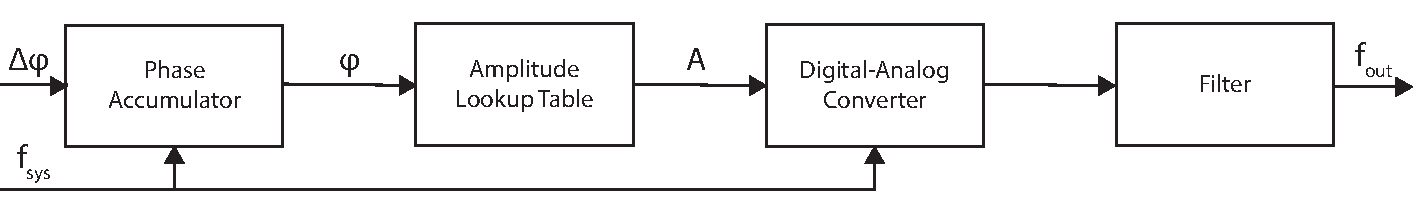
\includegraphics[width=\textwidth]
  {../figure/digital-signal-synthesis/simple-architecture.pdf}
  \caption{Signal flow through a simple \gls{dds}. The output frequency
    determines a phase step $\Delta\varphi$ by which the accumulator is incremented at each
    clock cycle. The value of the phase accumulator is used for amplitude
    lookup of the desired output signal shape. A \gls{dac} samples the output
    signal which then is filtered to smooth the discrete \gls{dac} output.
  }\label{fig:dds_simple_architecture}
\end{figure}
For every clock cycle the phase accumulator is incremented by $\Delta\varphi$.
On overflow of the accumulator a new signal period starts. The phase
accumulator value is used to lookup the corresponding amplitude value of the
desired output signal shape. For example one can use a lookup table with the
values of a sinusoidal output signal. Alternatively one can omit the lookup
table and output a sawtooth output signal by suppling the phase accumulator
output directly to the \gls{dac} or a square wave signal output by suppling
the most significant bit directly. Finally a \gls{dac} converts the digital
amplitude value to an analog signal. An optional analog filter can be used to
smooth the discrete output. \Cref{tab:dds_parameters} discloses system
parameters used for our \gls{dds} model and the \gls{ad9910} we use in our
setup~\cite{AD9910}. Except for the precision which in practice is not the
same accross the phase accumulator, lookup table and \gls{dac} our model
parameters are choosen to be similar to the ones used in the setup.
\begin{table}[htb]
  \centering
  \begin{tabular}{ccc}
    \toprule
    & Example & \gls{ad9910} \\
    \midrule
    Phase Accumulator Precision $N$ &
    \SI{8}{\bit} &
    \SI{32}{\bit} \\
    Digital-Analog-Converter Precision $P$ &
    \SI{14}{\bit} &
    \SI{8}{\bit} \\
    System Clock $f_\text{sys}$ &
    \SI{1}{\giga\hertz} &
    \SI{1}{\giga\hertz} \\
    Signal Frequency $f_\text{out}$ &
    \SI{100}{\mega\hertz} &
    \SI{100}{\mega\hertz} \\
    \bottomrule
  \end{tabular}
  \caption{System parameters used for our simplified \gls{dds} model and
    used in the \gls{ad9910}.
  }\label{tab:dds_parameters}
\end{table}
In \Cref{fig:dds_simple_output} the signal of our model \gls{dds} at different
processing stages with the model parameters from \cref{tab:dds_parameters} are
illustrated.
\begin{figure}[htb]
  \centering
  \begin{adjustbox}{width=\textwidth}
    %% Creator: Matplotlib, PGF backend
%%
%% To include the figure in your LaTeX document, write
%%   \input{<filename>.pgf}
%%
%% Make sure the required packages are loaded in your preamble
%%   \usepackage{pgf}
%%
%% Figures using additional raster images can only be included by \input if
%% they are in the same directory as the main LaTeX file. For loading figures
%% from other directories you can use the `import` package
%%   \usepackage{import}
%% and then include the figures with
%%   \import{<path to file>}{<filename>.pgf}
%%
%% Matplotlib used the following preamble
%%   \usepackage{amsmath}\usepackage{siunitx}\usepackage{lmodern}
%%   \usepackage{fontspec}
%%
\begingroup%
\makeatletter%
\begin{pgfpicture}%
\pgfpathrectangle{\pgfpointorigin}{\pgfqpoint{12.000000in}{8.000000in}}%
\pgfusepath{use as bounding box, clip}%
\begin{pgfscope}%
\pgfsetbuttcap%
\pgfsetmiterjoin%
\pgfsetlinewidth{0.000000pt}%
\definecolor{currentstroke}{rgb}{1.000000,1.000000,1.000000}%
\pgfsetstrokecolor{currentstroke}%
\pgfsetdash{}{0pt}%
\pgfpathmoveto{\pgfqpoint{0.000000in}{0.000000in}}%
\pgfpathlineto{\pgfqpoint{12.000000in}{0.000000in}}%
\pgfpathlineto{\pgfqpoint{12.000000in}{8.000000in}}%
\pgfpathlineto{\pgfqpoint{0.000000in}{8.000000in}}%
\pgfpathclose%
\pgfusepath{}%
\end{pgfscope}%
\begin{pgfscope}%
\pgfsetbuttcap%
\pgfsetmiterjoin%
\definecolor{currentfill}{rgb}{1.000000,1.000000,1.000000}%
\pgfsetfillcolor{currentfill}%
\pgfsetlinewidth{0.000000pt}%
\definecolor{currentstroke}{rgb}{0.000000,0.000000,0.000000}%
\pgfsetstrokecolor{currentstroke}%
\pgfsetstrokeopacity{0.000000}%
\pgfsetdash{}{0pt}%
\pgfpathmoveto{\pgfqpoint{1.500000in}{6.165581in}}%
\pgfpathlineto{\pgfqpoint{10.800000in}{6.165581in}}%
\pgfpathlineto{\pgfqpoint{10.800000in}{7.840000in}}%
\pgfpathlineto{\pgfqpoint{1.500000in}{7.840000in}}%
\pgfpathclose%
\pgfusepath{fill}%
\end{pgfscope}%
\begin{pgfscope}%
\pgfpathrectangle{\pgfqpoint{1.500000in}{6.165581in}}{\pgfqpoint{9.300000in}{1.674419in}}%
\pgfusepath{clip}%
\pgfsetbuttcap%
\pgfsetroundjoin%
\definecolor{currentfill}{rgb}{0.121569,0.466667,0.705882}%
\pgfsetfillcolor{currentfill}%
\pgfsetlinewidth{1.003750pt}%
\definecolor{currentstroke}{rgb}{0.121569,0.466667,0.705882}%
\pgfsetstrokecolor{currentstroke}%
\pgfsetdash{}{0pt}%
\pgfpathmoveto{\pgfqpoint{1.950324in}{6.350153in}}%
\pgfpathcurveto{\pgfqpoint{1.957691in}{6.350153in}}{\pgfqpoint{1.964757in}{6.353079in}}{\pgfqpoint{1.969966in}{6.358289in}}%
\pgfpathcurveto{\pgfqpoint{1.975175in}{6.363498in}}{\pgfqpoint{1.978102in}{6.370564in}}{\pgfqpoint{1.978102in}{6.377930in}}%
\pgfpathcurveto{\pgfqpoint{1.978102in}{6.385297in}}{\pgfqpoint{1.975175in}{6.392363in}}{\pgfqpoint{1.969966in}{6.397572in}}%
\pgfpathcurveto{\pgfqpoint{1.964757in}{6.402781in}}{\pgfqpoint{1.957691in}{6.405708in}}{\pgfqpoint{1.950324in}{6.405708in}}%
\pgfpathcurveto{\pgfqpoint{1.942958in}{6.405708in}}{\pgfqpoint{1.935892in}{6.402781in}}{\pgfqpoint{1.930682in}{6.397572in}}%
\pgfpathcurveto{\pgfqpoint{1.925473in}{6.392363in}}{\pgfqpoint{1.922547in}{6.385297in}}{\pgfqpoint{1.922547in}{6.377930in}}%
\pgfpathcurveto{\pgfqpoint{1.922547in}{6.370564in}}{\pgfqpoint{1.925473in}{6.363498in}}{\pgfqpoint{1.930682in}{6.358289in}}%
\pgfpathcurveto{\pgfqpoint{1.935892in}{6.353079in}}{\pgfqpoint{1.942958in}{6.350153in}}{\pgfqpoint{1.950324in}{6.350153in}}%
\pgfpathclose%
\pgfusepath{stroke,fill}%
\end{pgfscope}%
\begin{pgfscope}%
\pgfpathrectangle{\pgfqpoint{1.500000in}{6.165581in}}{\pgfqpoint{9.300000in}{1.674419in}}%
\pgfusepath{clip}%
\pgfsetbuttcap%
\pgfsetroundjoin%
\definecolor{currentfill}{rgb}{0.121569,0.466667,0.705882}%
\pgfsetfillcolor{currentfill}%
\pgfsetlinewidth{1.003750pt}%
\definecolor{currentstroke}{rgb}{0.121569,0.466667,0.705882}%
\pgfsetstrokecolor{currentstroke}%
\pgfsetdash{}{0pt}%
\pgfpathmoveto{\pgfqpoint{2.121740in}{6.511008in}}%
\pgfpathcurveto{\pgfqpoint{2.129106in}{6.511008in}}{\pgfqpoint{2.136172in}{6.513935in}}{\pgfqpoint{2.141382in}{6.519144in}}%
\pgfpathcurveto{\pgfqpoint{2.146591in}{6.524353in}}{\pgfqpoint{2.149517in}{6.531419in}}{\pgfqpoint{2.149517in}{6.538786in}}%
\pgfpathcurveto{\pgfqpoint{2.149517in}{6.546152in}}{\pgfqpoint{2.146591in}{6.553218in}}{\pgfqpoint{2.141382in}{6.558427in}}%
\pgfpathcurveto{\pgfqpoint{2.136172in}{6.563636in}}{\pgfqpoint{2.129106in}{6.566563in}}{\pgfqpoint{2.121740in}{6.566563in}}%
\pgfpathcurveto{\pgfqpoint{2.114373in}{6.566563in}}{\pgfqpoint{2.107307in}{6.563636in}}{\pgfqpoint{2.102098in}{6.558427in}}%
\pgfpathcurveto{\pgfqpoint{2.096889in}{6.553218in}}{\pgfqpoint{2.093962in}{6.546152in}}{\pgfqpoint{2.093962in}{6.538786in}}%
\pgfpathcurveto{\pgfqpoint{2.093962in}{6.531419in}}{\pgfqpoint{2.096889in}{6.524353in}}{\pgfqpoint{2.102098in}{6.519144in}}%
\pgfpathcurveto{\pgfqpoint{2.107307in}{6.513935in}}{\pgfqpoint{2.114373in}{6.511008in}}{\pgfqpoint{2.121740in}{6.511008in}}%
\pgfpathclose%
\pgfusepath{stroke,fill}%
\end{pgfscope}%
\begin{pgfscope}%
\pgfpathrectangle{\pgfqpoint{1.500000in}{6.165581in}}{\pgfqpoint{9.300000in}{1.674419in}}%
\pgfusepath{clip}%
\pgfsetbuttcap%
\pgfsetroundjoin%
\definecolor{currentfill}{rgb}{0.121569,0.466667,0.705882}%
\pgfsetfillcolor{currentfill}%
\pgfsetlinewidth{1.003750pt}%
\definecolor{currentstroke}{rgb}{0.121569,0.466667,0.705882}%
\pgfsetstrokecolor{currentstroke}%
\pgfsetdash{}{0pt}%
\pgfpathmoveto{\pgfqpoint{2.293155in}{6.671863in}}%
\pgfpathcurveto{\pgfqpoint{2.300522in}{6.671863in}}{\pgfqpoint{2.307588in}{6.674790in}}{\pgfqpoint{2.312797in}{6.679999in}}%
\pgfpathcurveto{\pgfqpoint{2.318006in}{6.685208in}}{\pgfqpoint{2.320933in}{6.692274in}}{\pgfqpoint{2.320933in}{6.699641in}}%
\pgfpathcurveto{\pgfqpoint{2.320933in}{6.707007in}}{\pgfqpoint{2.318006in}{6.714073in}}{\pgfqpoint{2.312797in}{6.719283in}}%
\pgfpathcurveto{\pgfqpoint{2.307588in}{6.724492in}}{\pgfqpoint{2.300522in}{6.727418in}}{\pgfqpoint{2.293155in}{6.727418in}}%
\pgfpathcurveto{\pgfqpoint{2.285788in}{6.727418in}}{\pgfqpoint{2.278722in}{6.724492in}}{\pgfqpoint{2.273513in}{6.719283in}}%
\pgfpathcurveto{\pgfqpoint{2.268304in}{6.714073in}}{\pgfqpoint{2.265377in}{6.707007in}}{\pgfqpoint{2.265377in}{6.699641in}}%
\pgfpathcurveto{\pgfqpoint{2.265377in}{6.692274in}}{\pgfqpoint{2.268304in}{6.685208in}}{\pgfqpoint{2.273513in}{6.679999in}}%
\pgfpathcurveto{\pgfqpoint{2.278722in}{6.674790in}}{\pgfqpoint{2.285788in}{6.671863in}}{\pgfqpoint{2.293155in}{6.671863in}}%
\pgfpathclose%
\pgfusepath{stroke,fill}%
\end{pgfscope}%
\begin{pgfscope}%
\pgfpathrectangle{\pgfqpoint{1.500000in}{6.165581in}}{\pgfqpoint{9.300000in}{1.674419in}}%
\pgfusepath{clip}%
\pgfsetbuttcap%
\pgfsetroundjoin%
\definecolor{currentfill}{rgb}{0.121569,0.466667,0.705882}%
\pgfsetfillcolor{currentfill}%
\pgfsetlinewidth{1.003750pt}%
\definecolor{currentstroke}{rgb}{0.121569,0.466667,0.705882}%
\pgfsetstrokecolor{currentstroke}%
\pgfsetdash{}{0pt}%
\pgfpathmoveto{\pgfqpoint{2.464570in}{6.832718in}}%
\pgfpathcurveto{\pgfqpoint{2.471937in}{6.832718in}}{\pgfqpoint{2.479003in}{6.835645in}}{\pgfqpoint{2.484212in}{6.840854in}}%
\pgfpathcurveto{\pgfqpoint{2.489421in}{6.846063in}}{\pgfqpoint{2.492348in}{6.853129in}}{\pgfqpoint{2.492348in}{6.860496in}}%
\pgfpathcurveto{\pgfqpoint{2.492348in}{6.867863in}}{\pgfqpoint{2.489421in}{6.874929in}}{\pgfqpoint{2.484212in}{6.880138in}}%
\pgfpathcurveto{\pgfqpoint{2.479003in}{6.885347in}}{\pgfqpoint{2.471937in}{6.888274in}}{\pgfqpoint{2.464570in}{6.888274in}}%
\pgfpathcurveto{\pgfqpoint{2.457204in}{6.888274in}}{\pgfqpoint{2.450138in}{6.885347in}}{\pgfqpoint{2.444928in}{6.880138in}}%
\pgfpathcurveto{\pgfqpoint{2.439719in}{6.874929in}}{\pgfqpoint{2.436793in}{6.867863in}}{\pgfqpoint{2.436793in}{6.860496in}}%
\pgfpathcurveto{\pgfqpoint{2.436793in}{6.853129in}}{\pgfqpoint{2.439719in}{6.846063in}}{\pgfqpoint{2.444928in}{6.840854in}}%
\pgfpathcurveto{\pgfqpoint{2.450138in}{6.835645in}}{\pgfqpoint{2.457204in}{6.832718in}}{\pgfqpoint{2.464570in}{6.832718in}}%
\pgfpathclose%
\pgfusepath{stroke,fill}%
\end{pgfscope}%
\begin{pgfscope}%
\pgfpathrectangle{\pgfqpoint{1.500000in}{6.165581in}}{\pgfqpoint{9.300000in}{1.674419in}}%
\pgfusepath{clip}%
\pgfsetbuttcap%
\pgfsetroundjoin%
\definecolor{currentfill}{rgb}{0.121569,0.466667,0.705882}%
\pgfsetfillcolor{currentfill}%
\pgfsetlinewidth{1.003750pt}%
\definecolor{currentstroke}{rgb}{0.121569,0.466667,0.705882}%
\pgfsetstrokecolor{currentstroke}%
\pgfsetdash{}{0pt}%
\pgfpathmoveto{\pgfqpoint{2.635986in}{6.993573in}}%
\pgfpathcurveto{\pgfqpoint{2.643352in}{6.993573in}}{\pgfqpoint{2.650418in}{6.996500in}}{\pgfqpoint{2.655628in}{7.001709in}}%
\pgfpathcurveto{\pgfqpoint{2.660837in}{7.006918in}}{\pgfqpoint{2.663763in}{7.013984in}}{\pgfqpoint{2.663763in}{7.021351in}}%
\pgfpathcurveto{\pgfqpoint{2.663763in}{7.028718in}}{\pgfqpoint{2.660837in}{7.035784in}}{\pgfqpoint{2.655628in}{7.040993in}}%
\pgfpathcurveto{\pgfqpoint{2.650418in}{7.046202in}}{\pgfqpoint{2.643352in}{7.049129in}}{\pgfqpoint{2.635986in}{7.049129in}}%
\pgfpathcurveto{\pgfqpoint{2.628619in}{7.049129in}}{\pgfqpoint{2.621553in}{7.046202in}}{\pgfqpoint{2.616344in}{7.040993in}}%
\pgfpathcurveto{\pgfqpoint{2.611135in}{7.035784in}}{\pgfqpoint{2.608208in}{7.028718in}}{\pgfqpoint{2.608208in}{7.021351in}}%
\pgfpathcurveto{\pgfqpoint{2.608208in}{7.013984in}}{\pgfqpoint{2.611135in}{7.006918in}}{\pgfqpoint{2.616344in}{7.001709in}}%
\pgfpathcurveto{\pgfqpoint{2.621553in}{6.996500in}}{\pgfqpoint{2.628619in}{6.993573in}}{\pgfqpoint{2.635986in}{6.993573in}}%
\pgfpathclose%
\pgfusepath{stroke,fill}%
\end{pgfscope}%
\begin{pgfscope}%
\pgfpathrectangle{\pgfqpoint{1.500000in}{6.165581in}}{\pgfqpoint{9.300000in}{1.674419in}}%
\pgfusepath{clip}%
\pgfsetbuttcap%
\pgfsetroundjoin%
\definecolor{currentfill}{rgb}{0.121569,0.466667,0.705882}%
\pgfsetfillcolor{currentfill}%
\pgfsetlinewidth{1.003750pt}%
\definecolor{currentstroke}{rgb}{0.121569,0.466667,0.705882}%
\pgfsetstrokecolor{currentstroke}%
\pgfsetdash{}{0pt}%
\pgfpathmoveto{\pgfqpoint{2.807401in}{7.154428in}}%
\pgfpathcurveto{\pgfqpoint{2.814768in}{7.154428in}}{\pgfqpoint{2.821834in}{7.157355in}}{\pgfqpoint{2.827043in}{7.162564in}}%
\pgfpathcurveto{\pgfqpoint{2.832252in}{7.167773in}}{\pgfqpoint{2.835179in}{7.174839in}}{\pgfqpoint{2.835179in}{7.182206in}}%
\pgfpathcurveto{\pgfqpoint{2.835179in}{7.189573in}}{\pgfqpoint{2.832252in}{7.196639in}}{\pgfqpoint{2.827043in}{7.201848in}}%
\pgfpathcurveto{\pgfqpoint{2.821834in}{7.207057in}}{\pgfqpoint{2.814768in}{7.209984in}}{\pgfqpoint{2.807401in}{7.209984in}}%
\pgfpathcurveto{\pgfqpoint{2.800034in}{7.209984in}}{\pgfqpoint{2.792968in}{7.207057in}}{\pgfqpoint{2.787759in}{7.201848in}}%
\pgfpathcurveto{\pgfqpoint{2.782550in}{7.196639in}}{\pgfqpoint{2.779623in}{7.189573in}}{\pgfqpoint{2.779623in}{7.182206in}}%
\pgfpathcurveto{\pgfqpoint{2.779623in}{7.174839in}}{\pgfqpoint{2.782550in}{7.167773in}}{\pgfqpoint{2.787759in}{7.162564in}}%
\pgfpathcurveto{\pgfqpoint{2.792968in}{7.157355in}}{\pgfqpoint{2.800034in}{7.154428in}}{\pgfqpoint{2.807401in}{7.154428in}}%
\pgfpathclose%
\pgfusepath{stroke,fill}%
\end{pgfscope}%
\begin{pgfscope}%
\pgfpathrectangle{\pgfqpoint{1.500000in}{6.165581in}}{\pgfqpoint{9.300000in}{1.674419in}}%
\pgfusepath{clip}%
\pgfsetbuttcap%
\pgfsetroundjoin%
\definecolor{currentfill}{rgb}{0.121569,0.466667,0.705882}%
\pgfsetfillcolor{currentfill}%
\pgfsetlinewidth{1.003750pt}%
\definecolor{currentstroke}{rgb}{0.121569,0.466667,0.705882}%
\pgfsetstrokecolor{currentstroke}%
\pgfsetdash{}{0pt}%
\pgfpathmoveto{\pgfqpoint{2.978816in}{7.315283in}}%
\pgfpathcurveto{\pgfqpoint{2.986183in}{7.315283in}}{\pgfqpoint{2.993249in}{7.318210in}}{\pgfqpoint{2.998458in}{7.323419in}}%
\pgfpathcurveto{\pgfqpoint{3.003667in}{7.328628in}}{\pgfqpoint{3.006594in}{7.335694in}}{\pgfqpoint{3.006594in}{7.343061in}}%
\pgfpathcurveto{\pgfqpoint{3.006594in}{7.350428in}}{\pgfqpoint{3.003667in}{7.357494in}}{\pgfqpoint{2.998458in}{7.362703in}}%
\pgfpathcurveto{\pgfqpoint{2.993249in}{7.367912in}}{\pgfqpoint{2.986183in}{7.370839in}}{\pgfqpoint{2.978816in}{7.370839in}}%
\pgfpathcurveto{\pgfqpoint{2.971450in}{7.370839in}}{\pgfqpoint{2.964384in}{7.367912in}}{\pgfqpoint{2.959174in}{7.362703in}}%
\pgfpathcurveto{\pgfqpoint{2.953965in}{7.357494in}}{\pgfqpoint{2.951039in}{7.350428in}}{\pgfqpoint{2.951039in}{7.343061in}}%
\pgfpathcurveto{\pgfqpoint{2.951039in}{7.335694in}}{\pgfqpoint{2.953965in}{7.328628in}}{\pgfqpoint{2.959174in}{7.323419in}}%
\pgfpathcurveto{\pgfqpoint{2.964384in}{7.318210in}}{\pgfqpoint{2.971450in}{7.315283in}}{\pgfqpoint{2.978816in}{7.315283in}}%
\pgfpathclose%
\pgfusepath{stroke,fill}%
\end{pgfscope}%
\begin{pgfscope}%
\pgfpathrectangle{\pgfqpoint{1.500000in}{6.165581in}}{\pgfqpoint{9.300000in}{1.674419in}}%
\pgfusepath{clip}%
\pgfsetbuttcap%
\pgfsetroundjoin%
\definecolor{currentfill}{rgb}{0.121569,0.466667,0.705882}%
\pgfsetfillcolor{currentfill}%
\pgfsetlinewidth{1.003750pt}%
\definecolor{currentstroke}{rgb}{0.121569,0.466667,0.705882}%
\pgfsetstrokecolor{currentstroke}%
\pgfsetdash{}{0pt}%
\pgfpathmoveto{\pgfqpoint{3.150232in}{7.476139in}}%
\pgfpathcurveto{\pgfqpoint{3.157598in}{7.476139in}}{\pgfqpoint{3.164664in}{7.479065in}}{\pgfqpoint{3.169874in}{7.484274in}}%
\pgfpathcurveto{\pgfqpoint{3.175083in}{7.489484in}}{\pgfqpoint{3.178009in}{7.496550in}}{\pgfqpoint{3.178009in}{7.503916in}}%
\pgfpathcurveto{\pgfqpoint{3.178009in}{7.511283in}}{\pgfqpoint{3.175083in}{7.518349in}}{\pgfqpoint{3.169874in}{7.523558in}}%
\pgfpathcurveto{\pgfqpoint{3.164664in}{7.528767in}}{\pgfqpoint{3.157598in}{7.531694in}}{\pgfqpoint{3.150232in}{7.531694in}}%
\pgfpathcurveto{\pgfqpoint{3.142865in}{7.531694in}}{\pgfqpoint{3.135799in}{7.528767in}}{\pgfqpoint{3.130590in}{7.523558in}}%
\pgfpathcurveto{\pgfqpoint{3.125381in}{7.518349in}}{\pgfqpoint{3.122454in}{7.511283in}}{\pgfqpoint{3.122454in}{7.503916in}}%
\pgfpathcurveto{\pgfqpoint{3.122454in}{7.496550in}}{\pgfqpoint{3.125381in}{7.489484in}}{\pgfqpoint{3.130590in}{7.484274in}}%
\pgfpathcurveto{\pgfqpoint{3.135799in}{7.479065in}}{\pgfqpoint{3.142865in}{7.476139in}}{\pgfqpoint{3.150232in}{7.476139in}}%
\pgfpathclose%
\pgfusepath{stroke,fill}%
\end{pgfscope}%
\begin{pgfscope}%
\pgfpathrectangle{\pgfqpoint{1.500000in}{6.165581in}}{\pgfqpoint{9.300000in}{1.674419in}}%
\pgfusepath{clip}%
\pgfsetbuttcap%
\pgfsetroundjoin%
\definecolor{currentfill}{rgb}{0.121569,0.466667,0.705882}%
\pgfsetfillcolor{currentfill}%
\pgfsetlinewidth{1.003750pt}%
\definecolor{currentstroke}{rgb}{0.121569,0.466667,0.705882}%
\pgfsetstrokecolor{currentstroke}%
\pgfsetdash{}{0pt}%
\pgfpathmoveto{\pgfqpoint{3.321647in}{7.636994in}}%
\pgfpathcurveto{\pgfqpoint{3.329014in}{7.636994in}}{\pgfqpoint{3.336080in}{7.639920in}}{\pgfqpoint{3.341289in}{7.645130in}}%
\pgfpathcurveto{\pgfqpoint{3.346498in}{7.650339in}}{\pgfqpoint{3.349425in}{7.657405in}}{\pgfqpoint{3.349425in}{7.664771in}}%
\pgfpathcurveto{\pgfqpoint{3.349425in}{7.672138in}}{\pgfqpoint{3.346498in}{7.679204in}}{\pgfqpoint{3.341289in}{7.684413in}}%
\pgfpathcurveto{\pgfqpoint{3.336080in}{7.689622in}}{\pgfqpoint{3.329014in}{7.692549in}}{\pgfqpoint{3.321647in}{7.692549in}}%
\pgfpathcurveto{\pgfqpoint{3.314280in}{7.692549in}}{\pgfqpoint{3.307214in}{7.689622in}}{\pgfqpoint{3.302005in}{7.684413in}}%
\pgfpathcurveto{\pgfqpoint{3.296796in}{7.679204in}}{\pgfqpoint{3.293869in}{7.672138in}}{\pgfqpoint{3.293869in}{7.664771in}}%
\pgfpathcurveto{\pgfqpoint{3.293869in}{7.657405in}}{\pgfqpoint{3.296796in}{7.650339in}}{\pgfqpoint{3.302005in}{7.645130in}}%
\pgfpathcurveto{\pgfqpoint{3.307214in}{7.639920in}}{\pgfqpoint{3.314280in}{7.636994in}}{\pgfqpoint{3.321647in}{7.636994in}}%
\pgfpathclose%
\pgfusepath{stroke,fill}%
\end{pgfscope}%
\begin{pgfscope}%
\pgfpathrectangle{\pgfqpoint{1.500000in}{6.165581in}}{\pgfqpoint{9.300000in}{1.674419in}}%
\pgfusepath{clip}%
\pgfsetbuttcap%
\pgfsetroundjoin%
\definecolor{currentfill}{rgb}{0.121569,0.466667,0.705882}%
\pgfsetfillcolor{currentfill}%
\pgfsetlinewidth{1.003750pt}%
\definecolor{currentstroke}{rgb}{0.121569,0.466667,0.705882}%
\pgfsetstrokecolor{currentstroke}%
\pgfsetdash{}{0pt}%
\pgfpathmoveto{\pgfqpoint{3.493062in}{6.214044in}}%
\pgfpathcurveto{\pgfqpoint{3.500429in}{6.214044in}}{\pgfqpoint{3.507495in}{6.216971in}}{\pgfqpoint{3.512704in}{6.222180in}}%
\pgfpathcurveto{\pgfqpoint{3.517913in}{6.227389in}}{\pgfqpoint{3.520840in}{6.234455in}}{\pgfqpoint{3.520840in}{6.241822in}}%
\pgfpathcurveto{\pgfqpoint{3.520840in}{6.249189in}}{\pgfqpoint{3.517913in}{6.256255in}}{\pgfqpoint{3.512704in}{6.261464in}}%
\pgfpathcurveto{\pgfqpoint{3.507495in}{6.266673in}}{\pgfqpoint{3.500429in}{6.269600in}}{\pgfqpoint{3.493062in}{6.269600in}}%
\pgfpathcurveto{\pgfqpoint{3.485696in}{6.269600in}}{\pgfqpoint{3.478630in}{6.266673in}}{\pgfqpoint{3.473420in}{6.261464in}}%
\pgfpathcurveto{\pgfqpoint{3.468211in}{6.256255in}}{\pgfqpoint{3.465285in}{6.249189in}}{\pgfqpoint{3.465285in}{6.241822in}}%
\pgfpathcurveto{\pgfqpoint{3.465285in}{6.234455in}}{\pgfqpoint{3.468211in}{6.227389in}}{\pgfqpoint{3.473420in}{6.222180in}}%
\pgfpathcurveto{\pgfqpoint{3.478630in}{6.216971in}}{\pgfqpoint{3.485696in}{6.214044in}}{\pgfqpoint{3.493062in}{6.214044in}}%
\pgfpathclose%
\pgfusepath{stroke,fill}%
\end{pgfscope}%
\begin{pgfscope}%
\pgfpathrectangle{\pgfqpoint{1.500000in}{6.165581in}}{\pgfqpoint{9.300000in}{1.674419in}}%
\pgfusepath{clip}%
\pgfsetbuttcap%
\pgfsetroundjoin%
\definecolor{currentfill}{rgb}{0.121569,0.466667,0.705882}%
\pgfsetfillcolor{currentfill}%
\pgfsetlinewidth{1.003750pt}%
\definecolor{currentstroke}{rgb}{0.121569,0.466667,0.705882}%
\pgfsetstrokecolor{currentstroke}%
\pgfsetdash{}{0pt}%
\pgfpathmoveto{\pgfqpoint{3.664478in}{6.374900in}}%
\pgfpathcurveto{\pgfqpoint{3.671844in}{6.374900in}}{\pgfqpoint{3.678910in}{6.377826in}}{\pgfqpoint{3.684120in}{6.383035in}}%
\pgfpathcurveto{\pgfqpoint{3.689329in}{6.388245in}}{\pgfqpoint{3.692255in}{6.395311in}}{\pgfqpoint{3.692255in}{6.402677in}}%
\pgfpathcurveto{\pgfqpoint{3.692255in}{6.410044in}}{\pgfqpoint{3.689329in}{6.417110in}}{\pgfqpoint{3.684120in}{6.422319in}}%
\pgfpathcurveto{\pgfqpoint{3.678910in}{6.427528in}}{\pgfqpoint{3.671844in}{6.430455in}}{\pgfqpoint{3.664478in}{6.430455in}}%
\pgfpathcurveto{\pgfqpoint{3.657111in}{6.430455in}}{\pgfqpoint{3.650045in}{6.427528in}}{\pgfqpoint{3.644836in}{6.422319in}}%
\pgfpathcurveto{\pgfqpoint{3.639627in}{6.417110in}}{\pgfqpoint{3.636700in}{6.410044in}}{\pgfqpoint{3.636700in}{6.402677in}}%
\pgfpathcurveto{\pgfqpoint{3.636700in}{6.395311in}}{\pgfqpoint{3.639627in}{6.388245in}}{\pgfqpoint{3.644836in}{6.383035in}}%
\pgfpathcurveto{\pgfqpoint{3.650045in}{6.377826in}}{\pgfqpoint{3.657111in}{6.374900in}}{\pgfqpoint{3.664478in}{6.374900in}}%
\pgfpathclose%
\pgfusepath{stroke,fill}%
\end{pgfscope}%
\begin{pgfscope}%
\pgfpathrectangle{\pgfqpoint{1.500000in}{6.165581in}}{\pgfqpoint{9.300000in}{1.674419in}}%
\pgfusepath{clip}%
\pgfsetbuttcap%
\pgfsetroundjoin%
\definecolor{currentfill}{rgb}{0.121569,0.466667,0.705882}%
\pgfsetfillcolor{currentfill}%
\pgfsetlinewidth{1.003750pt}%
\definecolor{currentstroke}{rgb}{0.121569,0.466667,0.705882}%
\pgfsetstrokecolor{currentstroke}%
\pgfsetdash{}{0pt}%
\pgfpathmoveto{\pgfqpoint{3.835893in}{6.535755in}}%
\pgfpathcurveto{\pgfqpoint{3.843260in}{6.535755in}}{\pgfqpoint{3.850326in}{6.538682in}}{\pgfqpoint{3.855535in}{6.543891in}}%
\pgfpathcurveto{\pgfqpoint{3.860744in}{6.549100in}}{\pgfqpoint{3.863671in}{6.556166in}}{\pgfqpoint{3.863671in}{6.563532in}}%
\pgfpathcurveto{\pgfqpoint{3.863671in}{6.570899in}}{\pgfqpoint{3.860744in}{6.577965in}}{\pgfqpoint{3.855535in}{6.583174in}}%
\pgfpathcurveto{\pgfqpoint{3.850326in}{6.588383in}}{\pgfqpoint{3.843260in}{6.591310in}}{\pgfqpoint{3.835893in}{6.591310in}}%
\pgfpathcurveto{\pgfqpoint{3.828526in}{6.591310in}}{\pgfqpoint{3.821460in}{6.588383in}}{\pgfqpoint{3.816251in}{6.583174in}}%
\pgfpathcurveto{\pgfqpoint{3.811042in}{6.577965in}}{\pgfqpoint{3.808115in}{6.570899in}}{\pgfqpoint{3.808115in}{6.563532in}}%
\pgfpathcurveto{\pgfqpoint{3.808115in}{6.556166in}}{\pgfqpoint{3.811042in}{6.549100in}}{\pgfqpoint{3.816251in}{6.543891in}}%
\pgfpathcurveto{\pgfqpoint{3.821460in}{6.538682in}}{\pgfqpoint{3.828526in}{6.535755in}}{\pgfqpoint{3.835893in}{6.535755in}}%
\pgfpathclose%
\pgfusepath{stroke,fill}%
\end{pgfscope}%
\begin{pgfscope}%
\pgfpathrectangle{\pgfqpoint{1.500000in}{6.165581in}}{\pgfqpoint{9.300000in}{1.674419in}}%
\pgfusepath{clip}%
\pgfsetbuttcap%
\pgfsetroundjoin%
\definecolor{currentfill}{rgb}{0.121569,0.466667,0.705882}%
\pgfsetfillcolor{currentfill}%
\pgfsetlinewidth{1.003750pt}%
\definecolor{currentstroke}{rgb}{0.121569,0.466667,0.705882}%
\pgfsetstrokecolor{currentstroke}%
\pgfsetdash{}{0pt}%
\pgfpathmoveto{\pgfqpoint{4.007308in}{6.696610in}}%
\pgfpathcurveto{\pgfqpoint{4.014675in}{6.696610in}}{\pgfqpoint{4.021741in}{6.699537in}}{\pgfqpoint{4.026950in}{6.704746in}}%
\pgfpathcurveto{\pgfqpoint{4.032159in}{6.709955in}}{\pgfqpoint{4.035086in}{6.717021in}}{\pgfqpoint{4.035086in}{6.724388in}}%
\pgfpathcurveto{\pgfqpoint{4.035086in}{6.731754in}}{\pgfqpoint{4.032159in}{6.738820in}}{\pgfqpoint{4.026950in}{6.744029in}}%
\pgfpathcurveto{\pgfqpoint{4.021741in}{6.749239in}}{\pgfqpoint{4.014675in}{6.752165in}}{\pgfqpoint{4.007308in}{6.752165in}}%
\pgfpathcurveto{\pgfqpoint{3.999942in}{6.752165in}}{\pgfqpoint{3.992876in}{6.749239in}}{\pgfqpoint{3.987666in}{6.744029in}}%
\pgfpathcurveto{\pgfqpoint{3.982457in}{6.738820in}}{\pgfqpoint{3.979531in}{6.731754in}}{\pgfqpoint{3.979531in}{6.724388in}}%
\pgfpathcurveto{\pgfqpoint{3.979531in}{6.717021in}}{\pgfqpoint{3.982457in}{6.709955in}}{\pgfqpoint{3.987666in}{6.704746in}}%
\pgfpathcurveto{\pgfqpoint{3.992876in}{6.699537in}}{\pgfqpoint{3.999942in}{6.696610in}}{\pgfqpoint{4.007308in}{6.696610in}}%
\pgfpathclose%
\pgfusepath{stroke,fill}%
\end{pgfscope}%
\begin{pgfscope}%
\pgfpathrectangle{\pgfqpoint{1.500000in}{6.165581in}}{\pgfqpoint{9.300000in}{1.674419in}}%
\pgfusepath{clip}%
\pgfsetbuttcap%
\pgfsetroundjoin%
\definecolor{currentfill}{rgb}{0.121569,0.466667,0.705882}%
\pgfsetfillcolor{currentfill}%
\pgfsetlinewidth{1.003750pt}%
\definecolor{currentstroke}{rgb}{0.121569,0.466667,0.705882}%
\pgfsetstrokecolor{currentstroke}%
\pgfsetdash{}{0pt}%
\pgfpathmoveto{\pgfqpoint{4.178724in}{6.857465in}}%
\pgfpathcurveto{\pgfqpoint{4.186090in}{6.857465in}}{\pgfqpoint{4.193156in}{6.860392in}}{\pgfqpoint{4.198366in}{6.865601in}}%
\pgfpathcurveto{\pgfqpoint{4.203575in}{6.870810in}}{\pgfqpoint{4.206501in}{6.877876in}}{\pgfqpoint{4.206501in}{6.885243in}}%
\pgfpathcurveto{\pgfqpoint{4.206501in}{6.892609in}}{\pgfqpoint{4.203575in}{6.899675in}}{\pgfqpoint{4.198366in}{6.904885in}}%
\pgfpathcurveto{\pgfqpoint{4.193156in}{6.910094in}}{\pgfqpoint{4.186090in}{6.913020in}}{\pgfqpoint{4.178724in}{6.913020in}}%
\pgfpathcurveto{\pgfqpoint{4.171357in}{6.913020in}}{\pgfqpoint{4.164291in}{6.910094in}}{\pgfqpoint{4.159082in}{6.904885in}}%
\pgfpathcurveto{\pgfqpoint{4.153873in}{6.899675in}}{\pgfqpoint{4.150946in}{6.892609in}}{\pgfqpoint{4.150946in}{6.885243in}}%
\pgfpathcurveto{\pgfqpoint{4.150946in}{6.877876in}}{\pgfqpoint{4.153873in}{6.870810in}}{\pgfqpoint{4.159082in}{6.865601in}}%
\pgfpathcurveto{\pgfqpoint{4.164291in}{6.860392in}}{\pgfqpoint{4.171357in}{6.857465in}}{\pgfqpoint{4.178724in}{6.857465in}}%
\pgfpathclose%
\pgfusepath{stroke,fill}%
\end{pgfscope}%
\begin{pgfscope}%
\pgfpathrectangle{\pgfqpoint{1.500000in}{6.165581in}}{\pgfqpoint{9.300000in}{1.674419in}}%
\pgfusepath{clip}%
\pgfsetbuttcap%
\pgfsetroundjoin%
\definecolor{currentfill}{rgb}{0.121569,0.466667,0.705882}%
\pgfsetfillcolor{currentfill}%
\pgfsetlinewidth{1.003750pt}%
\definecolor{currentstroke}{rgb}{0.121569,0.466667,0.705882}%
\pgfsetstrokecolor{currentstroke}%
\pgfsetdash{}{0pt}%
\pgfpathmoveto{\pgfqpoint{4.350139in}{7.018320in}}%
\pgfpathcurveto{\pgfqpoint{4.357506in}{7.018320in}}{\pgfqpoint{4.364572in}{7.021247in}}{\pgfqpoint{4.369781in}{7.026456in}}%
\pgfpathcurveto{\pgfqpoint{4.374990in}{7.031665in}}{\pgfqpoint{4.377917in}{7.038731in}}{\pgfqpoint{4.377917in}{7.046098in}}%
\pgfpathcurveto{\pgfqpoint{4.377917in}{7.053465in}}{\pgfqpoint{4.374990in}{7.060531in}}{\pgfqpoint{4.369781in}{7.065740in}}%
\pgfpathcurveto{\pgfqpoint{4.364572in}{7.070949in}}{\pgfqpoint{4.357506in}{7.073876in}}{\pgfqpoint{4.350139in}{7.073876in}}%
\pgfpathcurveto{\pgfqpoint{4.342772in}{7.073876in}}{\pgfqpoint{4.335706in}{7.070949in}}{\pgfqpoint{4.330497in}{7.065740in}}%
\pgfpathcurveto{\pgfqpoint{4.325288in}{7.060531in}}{\pgfqpoint{4.322361in}{7.053465in}}{\pgfqpoint{4.322361in}{7.046098in}}%
\pgfpathcurveto{\pgfqpoint{4.322361in}{7.038731in}}{\pgfqpoint{4.325288in}{7.031665in}}{\pgfqpoint{4.330497in}{7.026456in}}%
\pgfpathcurveto{\pgfqpoint{4.335706in}{7.021247in}}{\pgfqpoint{4.342772in}{7.018320in}}{\pgfqpoint{4.350139in}{7.018320in}}%
\pgfpathclose%
\pgfusepath{stroke,fill}%
\end{pgfscope}%
\begin{pgfscope}%
\pgfpathrectangle{\pgfqpoint{1.500000in}{6.165581in}}{\pgfqpoint{9.300000in}{1.674419in}}%
\pgfusepath{clip}%
\pgfsetbuttcap%
\pgfsetroundjoin%
\definecolor{currentfill}{rgb}{0.121569,0.466667,0.705882}%
\pgfsetfillcolor{currentfill}%
\pgfsetlinewidth{1.003750pt}%
\definecolor{currentstroke}{rgb}{0.121569,0.466667,0.705882}%
\pgfsetstrokecolor{currentstroke}%
\pgfsetdash{}{0pt}%
\pgfpathmoveto{\pgfqpoint{4.521554in}{7.179175in}}%
\pgfpathcurveto{\pgfqpoint{4.528921in}{7.179175in}}{\pgfqpoint{4.535987in}{7.182102in}}{\pgfqpoint{4.541196in}{7.187311in}}%
\pgfpathcurveto{\pgfqpoint{4.546405in}{7.192520in}}{\pgfqpoint{4.549332in}{7.199586in}}{\pgfqpoint{4.549332in}{7.206953in}}%
\pgfpathcurveto{\pgfqpoint{4.549332in}{7.214320in}}{\pgfqpoint{4.546405in}{7.221386in}}{\pgfqpoint{4.541196in}{7.226595in}}%
\pgfpathcurveto{\pgfqpoint{4.535987in}{7.231804in}}{\pgfqpoint{4.528921in}{7.234731in}}{\pgfqpoint{4.521554in}{7.234731in}}%
\pgfpathcurveto{\pgfqpoint{4.514188in}{7.234731in}}{\pgfqpoint{4.507122in}{7.231804in}}{\pgfqpoint{4.501912in}{7.226595in}}%
\pgfpathcurveto{\pgfqpoint{4.496703in}{7.221386in}}{\pgfqpoint{4.493777in}{7.214320in}}{\pgfqpoint{4.493777in}{7.206953in}}%
\pgfpathcurveto{\pgfqpoint{4.493777in}{7.199586in}}{\pgfqpoint{4.496703in}{7.192520in}}{\pgfqpoint{4.501912in}{7.187311in}}%
\pgfpathcurveto{\pgfqpoint{4.507122in}{7.182102in}}{\pgfqpoint{4.514188in}{7.179175in}}{\pgfqpoint{4.521554in}{7.179175in}}%
\pgfpathclose%
\pgfusepath{stroke,fill}%
\end{pgfscope}%
\begin{pgfscope}%
\pgfpathrectangle{\pgfqpoint{1.500000in}{6.165581in}}{\pgfqpoint{9.300000in}{1.674419in}}%
\pgfusepath{clip}%
\pgfsetbuttcap%
\pgfsetroundjoin%
\definecolor{currentfill}{rgb}{0.121569,0.466667,0.705882}%
\pgfsetfillcolor{currentfill}%
\pgfsetlinewidth{1.003750pt}%
\definecolor{currentstroke}{rgb}{0.121569,0.466667,0.705882}%
\pgfsetstrokecolor{currentstroke}%
\pgfsetdash{}{0pt}%
\pgfpathmoveto{\pgfqpoint{4.692970in}{7.340030in}}%
\pgfpathcurveto{\pgfqpoint{4.700336in}{7.340030in}}{\pgfqpoint{4.707402in}{7.342957in}}{\pgfqpoint{4.712612in}{7.348166in}}%
\pgfpathcurveto{\pgfqpoint{4.717821in}{7.353375in}}{\pgfqpoint{4.720747in}{7.360441in}}{\pgfqpoint{4.720747in}{7.367808in}}%
\pgfpathcurveto{\pgfqpoint{4.720747in}{7.375175in}}{\pgfqpoint{4.717821in}{7.382241in}}{\pgfqpoint{4.712612in}{7.387450in}}%
\pgfpathcurveto{\pgfqpoint{4.707402in}{7.392659in}}{\pgfqpoint{4.700336in}{7.395586in}}{\pgfqpoint{4.692970in}{7.395586in}}%
\pgfpathcurveto{\pgfqpoint{4.685603in}{7.395586in}}{\pgfqpoint{4.678537in}{7.392659in}}{\pgfqpoint{4.673328in}{7.387450in}}%
\pgfpathcurveto{\pgfqpoint{4.668119in}{7.382241in}}{\pgfqpoint{4.665192in}{7.375175in}}{\pgfqpoint{4.665192in}{7.367808in}}%
\pgfpathcurveto{\pgfqpoint{4.665192in}{7.360441in}}{\pgfqpoint{4.668119in}{7.353375in}}{\pgfqpoint{4.673328in}{7.348166in}}%
\pgfpathcurveto{\pgfqpoint{4.678537in}{7.342957in}}{\pgfqpoint{4.685603in}{7.340030in}}{\pgfqpoint{4.692970in}{7.340030in}}%
\pgfpathclose%
\pgfusepath{stroke,fill}%
\end{pgfscope}%
\begin{pgfscope}%
\pgfpathrectangle{\pgfqpoint{1.500000in}{6.165581in}}{\pgfqpoint{9.300000in}{1.674419in}}%
\pgfusepath{clip}%
\pgfsetbuttcap%
\pgfsetroundjoin%
\definecolor{currentfill}{rgb}{0.121569,0.466667,0.705882}%
\pgfsetfillcolor{currentfill}%
\pgfsetlinewidth{1.003750pt}%
\definecolor{currentstroke}{rgb}{0.121569,0.466667,0.705882}%
\pgfsetstrokecolor{currentstroke}%
\pgfsetdash{}{0pt}%
\pgfpathmoveto{\pgfqpoint{4.864385in}{7.500885in}}%
\pgfpathcurveto{\pgfqpoint{4.871752in}{7.500885in}}{\pgfqpoint{4.878818in}{7.503812in}}{\pgfqpoint{4.884027in}{7.509021in}}%
\pgfpathcurveto{\pgfqpoint{4.889236in}{7.514230in}}{\pgfqpoint{4.892163in}{7.521296in}}{\pgfqpoint{4.892163in}{7.528663in}}%
\pgfpathcurveto{\pgfqpoint{4.892163in}{7.536030in}}{\pgfqpoint{4.889236in}{7.543096in}}{\pgfqpoint{4.884027in}{7.548305in}}%
\pgfpathcurveto{\pgfqpoint{4.878818in}{7.553514in}}{\pgfqpoint{4.871752in}{7.556441in}}{\pgfqpoint{4.864385in}{7.556441in}}%
\pgfpathcurveto{\pgfqpoint{4.857018in}{7.556441in}}{\pgfqpoint{4.849952in}{7.553514in}}{\pgfqpoint{4.844743in}{7.548305in}}%
\pgfpathcurveto{\pgfqpoint{4.839534in}{7.543096in}}{\pgfqpoint{4.836607in}{7.536030in}}{\pgfqpoint{4.836607in}{7.528663in}}%
\pgfpathcurveto{\pgfqpoint{4.836607in}{7.521296in}}{\pgfqpoint{4.839534in}{7.514230in}}{\pgfqpoint{4.844743in}{7.509021in}}%
\pgfpathcurveto{\pgfqpoint{4.849952in}{7.503812in}}{\pgfqpoint{4.857018in}{7.500885in}}{\pgfqpoint{4.864385in}{7.500885in}}%
\pgfpathclose%
\pgfusepath{stroke,fill}%
\end{pgfscope}%
\begin{pgfscope}%
\pgfpathrectangle{\pgfqpoint{1.500000in}{6.165581in}}{\pgfqpoint{9.300000in}{1.674419in}}%
\pgfusepath{clip}%
\pgfsetbuttcap%
\pgfsetroundjoin%
\definecolor{currentfill}{rgb}{0.121569,0.466667,0.705882}%
\pgfsetfillcolor{currentfill}%
\pgfsetlinewidth{1.003750pt}%
\definecolor{currentstroke}{rgb}{0.121569,0.466667,0.705882}%
\pgfsetstrokecolor{currentstroke}%
\pgfsetdash{}{0pt}%
\pgfpathmoveto{\pgfqpoint{5.035800in}{7.661741in}}%
\pgfpathcurveto{\pgfqpoint{5.043167in}{7.661741in}}{\pgfqpoint{5.050233in}{7.664667in}}{\pgfqpoint{5.055442in}{7.669876in}}%
\pgfpathcurveto{\pgfqpoint{5.060651in}{7.675086in}}{\pgfqpoint{5.063578in}{7.682152in}}{\pgfqpoint{5.063578in}{7.689518in}}%
\pgfpathcurveto{\pgfqpoint{5.063578in}{7.696885in}}{\pgfqpoint{5.060651in}{7.703951in}}{\pgfqpoint{5.055442in}{7.709160in}}%
\pgfpathcurveto{\pgfqpoint{5.050233in}{7.714369in}}{\pgfqpoint{5.043167in}{7.717296in}}{\pgfqpoint{5.035800in}{7.717296in}}%
\pgfpathcurveto{\pgfqpoint{5.028434in}{7.717296in}}{\pgfqpoint{5.021368in}{7.714369in}}{\pgfqpoint{5.016158in}{7.709160in}}%
\pgfpathcurveto{\pgfqpoint{5.010949in}{7.703951in}}{\pgfqpoint{5.008023in}{7.696885in}}{\pgfqpoint{5.008023in}{7.689518in}}%
\pgfpathcurveto{\pgfqpoint{5.008023in}{7.682152in}}{\pgfqpoint{5.010949in}{7.675086in}}{\pgfqpoint{5.016158in}{7.669876in}}%
\pgfpathcurveto{\pgfqpoint{5.021368in}{7.664667in}}{\pgfqpoint{5.028434in}{7.661741in}}{\pgfqpoint{5.035800in}{7.661741in}}%
\pgfpathclose%
\pgfusepath{stroke,fill}%
\end{pgfscope}%
\begin{pgfscope}%
\pgfpathrectangle{\pgfqpoint{1.500000in}{6.165581in}}{\pgfqpoint{9.300000in}{1.674419in}}%
\pgfusepath{clip}%
\pgfsetbuttcap%
\pgfsetroundjoin%
\definecolor{currentfill}{rgb}{0.121569,0.466667,0.705882}%
\pgfsetfillcolor{currentfill}%
\pgfsetlinewidth{1.003750pt}%
\definecolor{currentstroke}{rgb}{0.121569,0.466667,0.705882}%
\pgfsetstrokecolor{currentstroke}%
\pgfsetdash{}{0pt}%
\pgfpathmoveto{\pgfqpoint{5.207216in}{6.238791in}}%
\pgfpathcurveto{\pgfqpoint{5.214582in}{6.238791in}}{\pgfqpoint{5.221648in}{6.241718in}}{\pgfqpoint{5.226858in}{6.246927in}}%
\pgfpathcurveto{\pgfqpoint{5.232067in}{6.252136in}}{\pgfqpoint{5.234993in}{6.259202in}}{\pgfqpoint{5.234993in}{6.266569in}}%
\pgfpathcurveto{\pgfqpoint{5.234993in}{6.273936in}}{\pgfqpoint{5.232067in}{6.281002in}}{\pgfqpoint{5.226858in}{6.286211in}}%
\pgfpathcurveto{\pgfqpoint{5.221648in}{6.291420in}}{\pgfqpoint{5.214582in}{6.294347in}}{\pgfqpoint{5.207216in}{6.294347in}}%
\pgfpathcurveto{\pgfqpoint{5.199849in}{6.294347in}}{\pgfqpoint{5.192783in}{6.291420in}}{\pgfqpoint{5.187574in}{6.286211in}}%
\pgfpathcurveto{\pgfqpoint{5.182365in}{6.281002in}}{\pgfqpoint{5.179438in}{6.273936in}}{\pgfqpoint{5.179438in}{6.266569in}}%
\pgfpathcurveto{\pgfqpoint{5.179438in}{6.259202in}}{\pgfqpoint{5.182365in}{6.252136in}}{\pgfqpoint{5.187574in}{6.246927in}}%
\pgfpathcurveto{\pgfqpoint{5.192783in}{6.241718in}}{\pgfqpoint{5.199849in}{6.238791in}}{\pgfqpoint{5.207216in}{6.238791in}}%
\pgfpathclose%
\pgfusepath{stroke,fill}%
\end{pgfscope}%
\begin{pgfscope}%
\pgfpathrectangle{\pgfqpoint{1.500000in}{6.165581in}}{\pgfqpoint{9.300000in}{1.674419in}}%
\pgfusepath{clip}%
\pgfsetbuttcap%
\pgfsetroundjoin%
\definecolor{currentfill}{rgb}{0.121569,0.466667,0.705882}%
\pgfsetfillcolor{currentfill}%
\pgfsetlinewidth{1.003750pt}%
\definecolor{currentstroke}{rgb}{0.121569,0.466667,0.705882}%
\pgfsetstrokecolor{currentstroke}%
\pgfsetdash{}{0pt}%
\pgfpathmoveto{\pgfqpoint{5.378631in}{6.399647in}}%
\pgfpathcurveto{\pgfqpoint{5.385998in}{6.399647in}}{\pgfqpoint{5.393064in}{6.402573in}}{\pgfqpoint{5.398273in}{6.407782in}}%
\pgfpathcurveto{\pgfqpoint{5.403482in}{6.412992in}}{\pgfqpoint{5.406409in}{6.420058in}}{\pgfqpoint{5.406409in}{6.427424in}}%
\pgfpathcurveto{\pgfqpoint{5.406409in}{6.434791in}}{\pgfqpoint{5.403482in}{6.441857in}}{\pgfqpoint{5.398273in}{6.447066in}}%
\pgfpathcurveto{\pgfqpoint{5.393064in}{6.452275in}}{\pgfqpoint{5.385998in}{6.455202in}}{\pgfqpoint{5.378631in}{6.455202in}}%
\pgfpathcurveto{\pgfqpoint{5.371264in}{6.455202in}}{\pgfqpoint{5.364198in}{6.452275in}}{\pgfqpoint{5.358989in}{6.447066in}}%
\pgfpathcurveto{\pgfqpoint{5.353780in}{6.441857in}}{\pgfqpoint{5.350853in}{6.434791in}}{\pgfqpoint{5.350853in}{6.427424in}}%
\pgfpathcurveto{\pgfqpoint{5.350853in}{6.420058in}}{\pgfqpoint{5.353780in}{6.412992in}}{\pgfqpoint{5.358989in}{6.407782in}}%
\pgfpathcurveto{\pgfqpoint{5.364198in}{6.402573in}}{\pgfqpoint{5.371264in}{6.399647in}}{\pgfqpoint{5.378631in}{6.399647in}}%
\pgfpathclose%
\pgfusepath{stroke,fill}%
\end{pgfscope}%
\begin{pgfscope}%
\pgfpathrectangle{\pgfqpoint{1.500000in}{6.165581in}}{\pgfqpoint{9.300000in}{1.674419in}}%
\pgfusepath{clip}%
\pgfsetbuttcap%
\pgfsetroundjoin%
\definecolor{currentfill}{rgb}{0.121569,0.466667,0.705882}%
\pgfsetfillcolor{currentfill}%
\pgfsetlinewidth{1.003750pt}%
\definecolor{currentstroke}{rgb}{0.121569,0.466667,0.705882}%
\pgfsetstrokecolor{currentstroke}%
\pgfsetdash{}{0pt}%
\pgfpathmoveto{\pgfqpoint{5.550046in}{6.560502in}}%
\pgfpathcurveto{\pgfqpoint{5.557413in}{6.560502in}}{\pgfqpoint{5.564479in}{6.563428in}}{\pgfqpoint{5.569688in}{6.568638in}}%
\pgfpathcurveto{\pgfqpoint{5.574897in}{6.573847in}}{\pgfqpoint{5.577824in}{6.580913in}}{\pgfqpoint{5.577824in}{6.588279in}}%
\pgfpathcurveto{\pgfqpoint{5.577824in}{6.595646in}}{\pgfqpoint{5.574897in}{6.602712in}}{\pgfqpoint{5.569688in}{6.607921in}}%
\pgfpathcurveto{\pgfqpoint{5.564479in}{6.613130in}}{\pgfqpoint{5.557413in}{6.616057in}}{\pgfqpoint{5.550046in}{6.616057in}}%
\pgfpathcurveto{\pgfqpoint{5.542680in}{6.616057in}}{\pgfqpoint{5.535614in}{6.613130in}}{\pgfqpoint{5.530404in}{6.607921in}}%
\pgfpathcurveto{\pgfqpoint{5.525195in}{6.602712in}}{\pgfqpoint{5.522269in}{6.595646in}}{\pgfqpoint{5.522269in}{6.588279in}}%
\pgfpathcurveto{\pgfqpoint{5.522269in}{6.580913in}}{\pgfqpoint{5.525195in}{6.573847in}}{\pgfqpoint{5.530404in}{6.568638in}}%
\pgfpathcurveto{\pgfqpoint{5.535614in}{6.563428in}}{\pgfqpoint{5.542680in}{6.560502in}}{\pgfqpoint{5.550046in}{6.560502in}}%
\pgfpathclose%
\pgfusepath{stroke,fill}%
\end{pgfscope}%
\begin{pgfscope}%
\pgfpathrectangle{\pgfqpoint{1.500000in}{6.165581in}}{\pgfqpoint{9.300000in}{1.674419in}}%
\pgfusepath{clip}%
\pgfsetbuttcap%
\pgfsetroundjoin%
\definecolor{currentfill}{rgb}{0.121569,0.466667,0.705882}%
\pgfsetfillcolor{currentfill}%
\pgfsetlinewidth{1.003750pt}%
\definecolor{currentstroke}{rgb}{0.121569,0.466667,0.705882}%
\pgfsetstrokecolor{currentstroke}%
\pgfsetdash{}{0pt}%
\pgfpathmoveto{\pgfqpoint{5.721462in}{6.721357in}}%
\pgfpathcurveto{\pgfqpoint{5.728828in}{6.721357in}}{\pgfqpoint{5.735894in}{6.724284in}}{\pgfqpoint{5.741104in}{6.729493in}}%
\pgfpathcurveto{\pgfqpoint{5.746313in}{6.734702in}}{\pgfqpoint{5.749239in}{6.741768in}}{\pgfqpoint{5.749239in}{6.749135in}}%
\pgfpathcurveto{\pgfqpoint{5.749239in}{6.756501in}}{\pgfqpoint{5.746313in}{6.763567in}}{\pgfqpoint{5.741104in}{6.768776in}}%
\pgfpathcurveto{\pgfqpoint{5.735894in}{6.773985in}}{\pgfqpoint{5.728828in}{6.776912in}}{\pgfqpoint{5.721462in}{6.776912in}}%
\pgfpathcurveto{\pgfqpoint{5.714095in}{6.776912in}}{\pgfqpoint{5.707029in}{6.773985in}}{\pgfqpoint{5.701820in}{6.768776in}}%
\pgfpathcurveto{\pgfqpoint{5.696611in}{6.763567in}}{\pgfqpoint{5.693684in}{6.756501in}}{\pgfqpoint{5.693684in}{6.749135in}}%
\pgfpathcurveto{\pgfqpoint{5.693684in}{6.741768in}}{\pgfqpoint{5.696611in}{6.734702in}}{\pgfqpoint{5.701820in}{6.729493in}}%
\pgfpathcurveto{\pgfqpoint{5.707029in}{6.724284in}}{\pgfqpoint{5.714095in}{6.721357in}}{\pgfqpoint{5.721462in}{6.721357in}}%
\pgfpathclose%
\pgfusepath{stroke,fill}%
\end{pgfscope}%
\begin{pgfscope}%
\pgfpathrectangle{\pgfqpoint{1.500000in}{6.165581in}}{\pgfqpoint{9.300000in}{1.674419in}}%
\pgfusepath{clip}%
\pgfsetbuttcap%
\pgfsetroundjoin%
\definecolor{currentfill}{rgb}{0.121569,0.466667,0.705882}%
\pgfsetfillcolor{currentfill}%
\pgfsetlinewidth{1.003750pt}%
\definecolor{currentstroke}{rgb}{0.121569,0.466667,0.705882}%
\pgfsetstrokecolor{currentstroke}%
\pgfsetdash{}{0pt}%
\pgfpathmoveto{\pgfqpoint{5.892877in}{6.882212in}}%
\pgfpathcurveto{\pgfqpoint{5.900244in}{6.882212in}}{\pgfqpoint{5.907310in}{6.885139in}}{\pgfqpoint{5.912519in}{6.890348in}}%
\pgfpathcurveto{\pgfqpoint{5.917728in}{6.895557in}}{\pgfqpoint{5.920655in}{6.902623in}}{\pgfqpoint{5.920655in}{6.909990in}}%
\pgfpathcurveto{\pgfqpoint{5.920655in}{6.917356in}}{\pgfqpoint{5.917728in}{6.924422in}}{\pgfqpoint{5.912519in}{6.929632in}}%
\pgfpathcurveto{\pgfqpoint{5.907310in}{6.934841in}}{\pgfqpoint{5.900244in}{6.937767in}}{\pgfqpoint{5.892877in}{6.937767in}}%
\pgfpathcurveto{\pgfqpoint{5.885510in}{6.937767in}}{\pgfqpoint{5.878444in}{6.934841in}}{\pgfqpoint{5.873235in}{6.929632in}}%
\pgfpathcurveto{\pgfqpoint{5.868026in}{6.924422in}}{\pgfqpoint{5.865099in}{6.917356in}}{\pgfqpoint{5.865099in}{6.909990in}}%
\pgfpathcurveto{\pgfqpoint{5.865099in}{6.902623in}}{\pgfqpoint{5.868026in}{6.895557in}}{\pgfqpoint{5.873235in}{6.890348in}}%
\pgfpathcurveto{\pgfqpoint{5.878444in}{6.885139in}}{\pgfqpoint{5.885510in}{6.882212in}}{\pgfqpoint{5.892877in}{6.882212in}}%
\pgfpathclose%
\pgfusepath{stroke,fill}%
\end{pgfscope}%
\begin{pgfscope}%
\pgfpathrectangle{\pgfqpoint{1.500000in}{6.165581in}}{\pgfqpoint{9.300000in}{1.674419in}}%
\pgfusepath{clip}%
\pgfsetbuttcap%
\pgfsetroundjoin%
\definecolor{currentfill}{rgb}{0.121569,0.466667,0.705882}%
\pgfsetfillcolor{currentfill}%
\pgfsetlinewidth{1.003750pt}%
\definecolor{currentstroke}{rgb}{0.121569,0.466667,0.705882}%
\pgfsetstrokecolor{currentstroke}%
\pgfsetdash{}{0pt}%
\pgfpathmoveto{\pgfqpoint{6.064292in}{7.043067in}}%
\pgfpathcurveto{\pgfqpoint{6.071659in}{7.043067in}}{\pgfqpoint{6.078725in}{7.045994in}}{\pgfqpoint{6.083934in}{7.051203in}}%
\pgfpathcurveto{\pgfqpoint{6.089143in}{7.056412in}}{\pgfqpoint{6.092070in}{7.063478in}}{\pgfqpoint{6.092070in}{7.070845in}}%
\pgfpathcurveto{\pgfqpoint{6.092070in}{7.078212in}}{\pgfqpoint{6.089143in}{7.085278in}}{\pgfqpoint{6.083934in}{7.090487in}}%
\pgfpathcurveto{\pgfqpoint{6.078725in}{7.095696in}}{\pgfqpoint{6.071659in}{7.098623in}}{\pgfqpoint{6.064292in}{7.098623in}}%
\pgfpathcurveto{\pgfqpoint{6.056926in}{7.098623in}}{\pgfqpoint{6.049860in}{7.095696in}}{\pgfqpoint{6.044650in}{7.090487in}}%
\pgfpathcurveto{\pgfqpoint{6.039441in}{7.085278in}}{\pgfqpoint{6.036515in}{7.078212in}}{\pgfqpoint{6.036515in}{7.070845in}}%
\pgfpathcurveto{\pgfqpoint{6.036515in}{7.063478in}}{\pgfqpoint{6.039441in}{7.056412in}}{\pgfqpoint{6.044650in}{7.051203in}}%
\pgfpathcurveto{\pgfqpoint{6.049860in}{7.045994in}}{\pgfqpoint{6.056926in}{7.043067in}}{\pgfqpoint{6.064292in}{7.043067in}}%
\pgfpathclose%
\pgfusepath{stroke,fill}%
\end{pgfscope}%
\begin{pgfscope}%
\pgfpathrectangle{\pgfqpoint{1.500000in}{6.165581in}}{\pgfqpoint{9.300000in}{1.674419in}}%
\pgfusepath{clip}%
\pgfsetbuttcap%
\pgfsetroundjoin%
\definecolor{currentfill}{rgb}{0.121569,0.466667,0.705882}%
\pgfsetfillcolor{currentfill}%
\pgfsetlinewidth{1.003750pt}%
\definecolor{currentstroke}{rgb}{0.121569,0.466667,0.705882}%
\pgfsetstrokecolor{currentstroke}%
\pgfsetdash{}{0pt}%
\pgfpathmoveto{\pgfqpoint{6.235708in}{7.203922in}}%
\pgfpathcurveto{\pgfqpoint{6.243074in}{7.203922in}}{\pgfqpoint{6.250140in}{7.206849in}}{\pgfqpoint{6.255350in}{7.212058in}}%
\pgfpathcurveto{\pgfqpoint{6.260559in}{7.217267in}}{\pgfqpoint{6.263485in}{7.224333in}}{\pgfqpoint{6.263485in}{7.231700in}}%
\pgfpathcurveto{\pgfqpoint{6.263485in}{7.239067in}}{\pgfqpoint{6.260559in}{7.246133in}}{\pgfqpoint{6.255350in}{7.251342in}}%
\pgfpathcurveto{\pgfqpoint{6.250140in}{7.256551in}}{\pgfqpoint{6.243074in}{7.259478in}}{\pgfqpoint{6.235708in}{7.259478in}}%
\pgfpathcurveto{\pgfqpoint{6.228341in}{7.259478in}}{\pgfqpoint{6.221275in}{7.256551in}}{\pgfqpoint{6.216066in}{7.251342in}}%
\pgfpathcurveto{\pgfqpoint{6.210857in}{7.246133in}}{\pgfqpoint{6.207930in}{7.239067in}}{\pgfqpoint{6.207930in}{7.231700in}}%
\pgfpathcurveto{\pgfqpoint{6.207930in}{7.224333in}}{\pgfqpoint{6.210857in}{7.217267in}}{\pgfqpoint{6.216066in}{7.212058in}}%
\pgfpathcurveto{\pgfqpoint{6.221275in}{7.206849in}}{\pgfqpoint{6.228341in}{7.203922in}}{\pgfqpoint{6.235708in}{7.203922in}}%
\pgfpathclose%
\pgfusepath{stroke,fill}%
\end{pgfscope}%
\begin{pgfscope}%
\pgfpathrectangle{\pgfqpoint{1.500000in}{6.165581in}}{\pgfqpoint{9.300000in}{1.674419in}}%
\pgfusepath{clip}%
\pgfsetbuttcap%
\pgfsetroundjoin%
\definecolor{currentfill}{rgb}{0.121569,0.466667,0.705882}%
\pgfsetfillcolor{currentfill}%
\pgfsetlinewidth{1.003750pt}%
\definecolor{currentstroke}{rgb}{0.121569,0.466667,0.705882}%
\pgfsetstrokecolor{currentstroke}%
\pgfsetdash{}{0pt}%
\pgfpathmoveto{\pgfqpoint{6.407123in}{7.364777in}}%
\pgfpathcurveto{\pgfqpoint{6.414490in}{7.364777in}}{\pgfqpoint{6.421556in}{7.367704in}}{\pgfqpoint{6.426765in}{7.372913in}}%
\pgfpathcurveto{\pgfqpoint{6.431974in}{7.378122in}}{\pgfqpoint{6.434901in}{7.385188in}}{\pgfqpoint{6.434901in}{7.392555in}}%
\pgfpathcurveto{\pgfqpoint{6.434901in}{7.399922in}}{\pgfqpoint{6.431974in}{7.406988in}}{\pgfqpoint{6.426765in}{7.412197in}}%
\pgfpathcurveto{\pgfqpoint{6.421556in}{7.417406in}}{\pgfqpoint{6.414490in}{7.420333in}}{\pgfqpoint{6.407123in}{7.420333in}}%
\pgfpathcurveto{\pgfqpoint{6.399756in}{7.420333in}}{\pgfqpoint{6.392690in}{7.417406in}}{\pgfqpoint{6.387481in}{7.412197in}}%
\pgfpathcurveto{\pgfqpoint{6.382272in}{7.406988in}}{\pgfqpoint{6.379345in}{7.399922in}}{\pgfqpoint{6.379345in}{7.392555in}}%
\pgfpathcurveto{\pgfqpoint{6.379345in}{7.385188in}}{\pgfqpoint{6.382272in}{7.378122in}}{\pgfqpoint{6.387481in}{7.372913in}}%
\pgfpathcurveto{\pgfqpoint{6.392690in}{7.367704in}}{\pgfqpoint{6.399756in}{7.364777in}}{\pgfqpoint{6.407123in}{7.364777in}}%
\pgfpathclose%
\pgfusepath{stroke,fill}%
\end{pgfscope}%
\begin{pgfscope}%
\pgfpathrectangle{\pgfqpoint{1.500000in}{6.165581in}}{\pgfqpoint{9.300000in}{1.674419in}}%
\pgfusepath{clip}%
\pgfsetbuttcap%
\pgfsetroundjoin%
\definecolor{currentfill}{rgb}{0.121569,0.466667,0.705882}%
\pgfsetfillcolor{currentfill}%
\pgfsetlinewidth{1.003750pt}%
\definecolor{currentstroke}{rgb}{0.121569,0.466667,0.705882}%
\pgfsetstrokecolor{currentstroke}%
\pgfsetdash{}{0pt}%
\pgfpathmoveto{\pgfqpoint{6.578538in}{7.525632in}}%
\pgfpathcurveto{\pgfqpoint{6.585905in}{7.525632in}}{\pgfqpoint{6.592971in}{7.528559in}}{\pgfqpoint{6.598180in}{7.533768in}}%
\pgfpathcurveto{\pgfqpoint{6.603389in}{7.538977in}}{\pgfqpoint{6.606316in}{7.546043in}}{\pgfqpoint{6.606316in}{7.553410in}}%
\pgfpathcurveto{\pgfqpoint{6.606316in}{7.560777in}}{\pgfqpoint{6.603389in}{7.567843in}}{\pgfqpoint{6.598180in}{7.573052in}}%
\pgfpathcurveto{\pgfqpoint{6.592971in}{7.578261in}}{\pgfqpoint{6.585905in}{7.581188in}}{\pgfqpoint{6.578538in}{7.581188in}}%
\pgfpathcurveto{\pgfqpoint{6.571172in}{7.581188in}}{\pgfqpoint{6.564106in}{7.578261in}}{\pgfqpoint{6.558896in}{7.573052in}}%
\pgfpathcurveto{\pgfqpoint{6.553687in}{7.567843in}}{\pgfqpoint{6.550761in}{7.560777in}}{\pgfqpoint{6.550761in}{7.553410in}}%
\pgfpathcurveto{\pgfqpoint{6.550761in}{7.546043in}}{\pgfqpoint{6.553687in}{7.538977in}}{\pgfqpoint{6.558896in}{7.533768in}}%
\pgfpathcurveto{\pgfqpoint{6.564106in}{7.528559in}}{\pgfqpoint{6.571172in}{7.525632in}}{\pgfqpoint{6.578538in}{7.525632in}}%
\pgfpathclose%
\pgfusepath{stroke,fill}%
\end{pgfscope}%
\begin{pgfscope}%
\pgfpathrectangle{\pgfqpoint{1.500000in}{6.165581in}}{\pgfqpoint{9.300000in}{1.674419in}}%
\pgfusepath{clip}%
\pgfsetbuttcap%
\pgfsetroundjoin%
\definecolor{currentfill}{rgb}{0.121569,0.466667,0.705882}%
\pgfsetfillcolor{currentfill}%
\pgfsetlinewidth{1.003750pt}%
\definecolor{currentstroke}{rgb}{0.121569,0.466667,0.705882}%
\pgfsetstrokecolor{currentstroke}%
\pgfsetdash{}{0pt}%
\pgfpathmoveto{\pgfqpoint{6.749954in}{7.686488in}}%
\pgfpathcurveto{\pgfqpoint{6.757320in}{7.686488in}}{\pgfqpoint{6.764386in}{7.689414in}}{\pgfqpoint{6.769596in}{7.694623in}}%
\pgfpathcurveto{\pgfqpoint{6.774805in}{7.699833in}}{\pgfqpoint{6.777731in}{7.706899in}}{\pgfqpoint{6.777731in}{7.714265in}}%
\pgfpathcurveto{\pgfqpoint{6.777731in}{7.721632in}}{\pgfqpoint{6.774805in}{7.728698in}}{\pgfqpoint{6.769596in}{7.733907in}}%
\pgfpathcurveto{\pgfqpoint{6.764386in}{7.739116in}}{\pgfqpoint{6.757320in}{7.742043in}}{\pgfqpoint{6.749954in}{7.742043in}}%
\pgfpathcurveto{\pgfqpoint{6.742587in}{7.742043in}}{\pgfqpoint{6.735521in}{7.739116in}}{\pgfqpoint{6.730312in}{7.733907in}}%
\pgfpathcurveto{\pgfqpoint{6.725103in}{7.728698in}}{\pgfqpoint{6.722176in}{7.721632in}}{\pgfqpoint{6.722176in}{7.714265in}}%
\pgfpathcurveto{\pgfqpoint{6.722176in}{7.706899in}}{\pgfqpoint{6.725103in}{7.699833in}}{\pgfqpoint{6.730312in}{7.694623in}}%
\pgfpathcurveto{\pgfqpoint{6.735521in}{7.689414in}}{\pgfqpoint{6.742587in}{7.686488in}}{\pgfqpoint{6.749954in}{7.686488in}}%
\pgfpathclose%
\pgfusepath{stroke,fill}%
\end{pgfscope}%
\begin{pgfscope}%
\pgfpathrectangle{\pgfqpoint{1.500000in}{6.165581in}}{\pgfqpoint{9.300000in}{1.674419in}}%
\pgfusepath{clip}%
\pgfsetbuttcap%
\pgfsetroundjoin%
\definecolor{currentfill}{rgb}{0.121569,0.466667,0.705882}%
\pgfsetfillcolor{currentfill}%
\pgfsetlinewidth{1.003750pt}%
\definecolor{currentstroke}{rgb}{0.121569,0.466667,0.705882}%
\pgfsetstrokecolor{currentstroke}%
\pgfsetdash{}{0pt}%
\pgfpathmoveto{\pgfqpoint{6.921369in}{6.263538in}}%
\pgfpathcurveto{\pgfqpoint{6.928736in}{6.263538in}}{\pgfqpoint{6.935802in}{6.266465in}}{\pgfqpoint{6.941011in}{6.271674in}}%
\pgfpathcurveto{\pgfqpoint{6.946220in}{6.276883in}}{\pgfqpoint{6.949147in}{6.283949in}}{\pgfqpoint{6.949147in}{6.291316in}}%
\pgfpathcurveto{\pgfqpoint{6.949147in}{6.298683in}}{\pgfqpoint{6.946220in}{6.305749in}}{\pgfqpoint{6.941011in}{6.310958in}}%
\pgfpathcurveto{\pgfqpoint{6.935802in}{6.316167in}}{\pgfqpoint{6.928736in}{6.319094in}}{\pgfqpoint{6.921369in}{6.319094in}}%
\pgfpathcurveto{\pgfqpoint{6.914002in}{6.319094in}}{\pgfqpoint{6.906936in}{6.316167in}}{\pgfqpoint{6.901727in}{6.310958in}}%
\pgfpathcurveto{\pgfqpoint{6.896518in}{6.305749in}}{\pgfqpoint{6.893591in}{6.298683in}}{\pgfqpoint{6.893591in}{6.291316in}}%
\pgfpathcurveto{\pgfqpoint{6.893591in}{6.283949in}}{\pgfqpoint{6.896518in}{6.276883in}}{\pgfqpoint{6.901727in}{6.271674in}}%
\pgfpathcurveto{\pgfqpoint{6.906936in}{6.266465in}}{\pgfqpoint{6.914002in}{6.263538in}}{\pgfqpoint{6.921369in}{6.263538in}}%
\pgfpathclose%
\pgfusepath{stroke,fill}%
\end{pgfscope}%
\begin{pgfscope}%
\pgfpathrectangle{\pgfqpoint{1.500000in}{6.165581in}}{\pgfqpoint{9.300000in}{1.674419in}}%
\pgfusepath{clip}%
\pgfsetbuttcap%
\pgfsetroundjoin%
\definecolor{currentfill}{rgb}{0.121569,0.466667,0.705882}%
\pgfsetfillcolor{currentfill}%
\pgfsetlinewidth{1.003750pt}%
\definecolor{currentstroke}{rgb}{0.121569,0.466667,0.705882}%
\pgfsetstrokecolor{currentstroke}%
\pgfsetdash{}{0pt}%
\pgfpathmoveto{\pgfqpoint{7.092784in}{6.424393in}}%
\pgfpathcurveto{\pgfqpoint{7.100151in}{6.424393in}}{\pgfqpoint{7.107217in}{6.427320in}}{\pgfqpoint{7.112426in}{6.432529in}}%
\pgfpathcurveto{\pgfqpoint{7.117635in}{6.437738in}}{\pgfqpoint{7.120562in}{6.444804in}}{\pgfqpoint{7.120562in}{6.452171in}}%
\pgfpathcurveto{\pgfqpoint{7.120562in}{6.459538in}}{\pgfqpoint{7.117635in}{6.466604in}}{\pgfqpoint{7.112426in}{6.471813in}}%
\pgfpathcurveto{\pgfqpoint{7.107217in}{6.477022in}}{\pgfqpoint{7.100151in}{6.479949in}}{\pgfqpoint{7.092784in}{6.479949in}}%
\pgfpathcurveto{\pgfqpoint{7.085418in}{6.479949in}}{\pgfqpoint{7.078352in}{6.477022in}}{\pgfqpoint{7.073142in}{6.471813in}}%
\pgfpathcurveto{\pgfqpoint{7.067933in}{6.466604in}}{\pgfqpoint{7.065007in}{6.459538in}}{\pgfqpoint{7.065007in}{6.452171in}}%
\pgfpathcurveto{\pgfqpoint{7.065007in}{6.444804in}}{\pgfqpoint{7.067933in}{6.437738in}}{\pgfqpoint{7.073142in}{6.432529in}}%
\pgfpathcurveto{\pgfqpoint{7.078352in}{6.427320in}}{\pgfqpoint{7.085418in}{6.424393in}}{\pgfqpoint{7.092784in}{6.424393in}}%
\pgfpathclose%
\pgfusepath{stroke,fill}%
\end{pgfscope}%
\begin{pgfscope}%
\pgfpathrectangle{\pgfqpoint{1.500000in}{6.165581in}}{\pgfqpoint{9.300000in}{1.674419in}}%
\pgfusepath{clip}%
\pgfsetbuttcap%
\pgfsetroundjoin%
\definecolor{currentfill}{rgb}{0.121569,0.466667,0.705882}%
\pgfsetfillcolor{currentfill}%
\pgfsetlinewidth{1.003750pt}%
\definecolor{currentstroke}{rgb}{0.121569,0.466667,0.705882}%
\pgfsetstrokecolor{currentstroke}%
\pgfsetdash{}{0pt}%
\pgfpathmoveto{\pgfqpoint{7.264200in}{6.585249in}}%
\pgfpathcurveto{\pgfqpoint{7.271566in}{6.585249in}}{\pgfqpoint{7.278632in}{6.588175in}}{\pgfqpoint{7.283842in}{6.593384in}}%
\pgfpathcurveto{\pgfqpoint{7.289051in}{6.598594in}}{\pgfqpoint{7.291977in}{6.605660in}}{\pgfqpoint{7.291977in}{6.613026in}}%
\pgfpathcurveto{\pgfqpoint{7.291977in}{6.620393in}}{\pgfqpoint{7.289051in}{6.627459in}}{\pgfqpoint{7.283842in}{6.632668in}}%
\pgfpathcurveto{\pgfqpoint{7.278632in}{6.637877in}}{\pgfqpoint{7.271566in}{6.640804in}}{\pgfqpoint{7.264200in}{6.640804in}}%
\pgfpathcurveto{\pgfqpoint{7.256833in}{6.640804in}}{\pgfqpoint{7.249767in}{6.637877in}}{\pgfqpoint{7.244558in}{6.632668in}}%
\pgfpathcurveto{\pgfqpoint{7.239349in}{6.627459in}}{\pgfqpoint{7.236422in}{6.620393in}}{\pgfqpoint{7.236422in}{6.613026in}}%
\pgfpathcurveto{\pgfqpoint{7.236422in}{6.605660in}}{\pgfqpoint{7.239349in}{6.598594in}}{\pgfqpoint{7.244558in}{6.593384in}}%
\pgfpathcurveto{\pgfqpoint{7.249767in}{6.588175in}}{\pgfqpoint{7.256833in}{6.585249in}}{\pgfqpoint{7.264200in}{6.585249in}}%
\pgfpathclose%
\pgfusepath{stroke,fill}%
\end{pgfscope}%
\begin{pgfscope}%
\pgfpathrectangle{\pgfqpoint{1.500000in}{6.165581in}}{\pgfqpoint{9.300000in}{1.674419in}}%
\pgfusepath{clip}%
\pgfsetbuttcap%
\pgfsetroundjoin%
\definecolor{currentfill}{rgb}{0.121569,0.466667,0.705882}%
\pgfsetfillcolor{currentfill}%
\pgfsetlinewidth{1.003750pt}%
\definecolor{currentstroke}{rgb}{0.121569,0.466667,0.705882}%
\pgfsetstrokecolor{currentstroke}%
\pgfsetdash{}{0pt}%
\pgfpathmoveto{\pgfqpoint{7.435615in}{6.746104in}}%
\pgfpathcurveto{\pgfqpoint{7.442982in}{6.746104in}}{\pgfqpoint{7.450048in}{6.749031in}}{\pgfqpoint{7.455257in}{6.754240in}}%
\pgfpathcurveto{\pgfqpoint{7.460466in}{6.759449in}}{\pgfqpoint{7.463393in}{6.766515in}}{\pgfqpoint{7.463393in}{6.773881in}}%
\pgfpathcurveto{\pgfqpoint{7.463393in}{6.781248in}}{\pgfqpoint{7.460466in}{6.788314in}}{\pgfqpoint{7.455257in}{6.793523in}}%
\pgfpathcurveto{\pgfqpoint{7.450048in}{6.798732in}}{\pgfqpoint{7.442982in}{6.801659in}}{\pgfqpoint{7.435615in}{6.801659in}}%
\pgfpathcurveto{\pgfqpoint{7.428248in}{6.801659in}}{\pgfqpoint{7.421182in}{6.798732in}}{\pgfqpoint{7.415973in}{6.793523in}}%
\pgfpathcurveto{\pgfqpoint{7.410764in}{6.788314in}}{\pgfqpoint{7.407837in}{6.781248in}}{\pgfqpoint{7.407837in}{6.773881in}}%
\pgfpathcurveto{\pgfqpoint{7.407837in}{6.766515in}}{\pgfqpoint{7.410764in}{6.759449in}}{\pgfqpoint{7.415973in}{6.754240in}}%
\pgfpathcurveto{\pgfqpoint{7.421182in}{6.749031in}}{\pgfqpoint{7.428248in}{6.746104in}}{\pgfqpoint{7.435615in}{6.746104in}}%
\pgfpathclose%
\pgfusepath{stroke,fill}%
\end{pgfscope}%
\begin{pgfscope}%
\pgfpathrectangle{\pgfqpoint{1.500000in}{6.165581in}}{\pgfqpoint{9.300000in}{1.674419in}}%
\pgfusepath{clip}%
\pgfsetbuttcap%
\pgfsetroundjoin%
\definecolor{currentfill}{rgb}{0.121569,0.466667,0.705882}%
\pgfsetfillcolor{currentfill}%
\pgfsetlinewidth{1.003750pt}%
\definecolor{currentstroke}{rgb}{0.121569,0.466667,0.705882}%
\pgfsetstrokecolor{currentstroke}%
\pgfsetdash{}{0pt}%
\pgfpathmoveto{\pgfqpoint{7.607030in}{6.906959in}}%
\pgfpathcurveto{\pgfqpoint{7.614397in}{6.906959in}}{\pgfqpoint{7.621463in}{6.909886in}}{\pgfqpoint{7.626672in}{6.915095in}}%
\pgfpathcurveto{\pgfqpoint{7.631881in}{6.920304in}}{\pgfqpoint{7.634808in}{6.927370in}}{\pgfqpoint{7.634808in}{6.934737in}}%
\pgfpathcurveto{\pgfqpoint{7.634808in}{6.942103in}}{\pgfqpoint{7.631881in}{6.949169in}}{\pgfqpoint{7.626672in}{6.954378in}}%
\pgfpathcurveto{\pgfqpoint{7.621463in}{6.959588in}}{\pgfqpoint{7.614397in}{6.962514in}}{\pgfqpoint{7.607030in}{6.962514in}}%
\pgfpathcurveto{\pgfqpoint{7.599664in}{6.962514in}}{\pgfqpoint{7.592598in}{6.959588in}}{\pgfqpoint{7.587388in}{6.954378in}}%
\pgfpathcurveto{\pgfqpoint{7.582179in}{6.949169in}}{\pgfqpoint{7.579253in}{6.942103in}}{\pgfqpoint{7.579253in}{6.934737in}}%
\pgfpathcurveto{\pgfqpoint{7.579253in}{6.927370in}}{\pgfqpoint{7.582179in}{6.920304in}}{\pgfqpoint{7.587388in}{6.915095in}}%
\pgfpathcurveto{\pgfqpoint{7.592598in}{6.909886in}}{\pgfqpoint{7.599664in}{6.906959in}}{\pgfqpoint{7.607030in}{6.906959in}}%
\pgfpathclose%
\pgfusepath{stroke,fill}%
\end{pgfscope}%
\begin{pgfscope}%
\pgfpathrectangle{\pgfqpoint{1.500000in}{6.165581in}}{\pgfqpoint{9.300000in}{1.674419in}}%
\pgfusepath{clip}%
\pgfsetbuttcap%
\pgfsetroundjoin%
\definecolor{currentfill}{rgb}{0.121569,0.466667,0.705882}%
\pgfsetfillcolor{currentfill}%
\pgfsetlinewidth{1.003750pt}%
\definecolor{currentstroke}{rgb}{0.121569,0.466667,0.705882}%
\pgfsetstrokecolor{currentstroke}%
\pgfsetdash{}{0pt}%
\pgfpathmoveto{\pgfqpoint{7.778446in}{7.067814in}}%
\pgfpathcurveto{\pgfqpoint{7.785812in}{7.067814in}}{\pgfqpoint{7.792878in}{7.070741in}}{\pgfqpoint{7.798088in}{7.075950in}}%
\pgfpathcurveto{\pgfqpoint{7.803297in}{7.081159in}}{\pgfqpoint{7.806223in}{7.088225in}}{\pgfqpoint{7.806223in}{7.095592in}}%
\pgfpathcurveto{\pgfqpoint{7.806223in}{7.102958in}}{\pgfqpoint{7.803297in}{7.110025in}}{\pgfqpoint{7.798088in}{7.115234in}}%
\pgfpathcurveto{\pgfqpoint{7.792878in}{7.120443in}}{\pgfqpoint{7.785812in}{7.123370in}}{\pgfqpoint{7.778446in}{7.123370in}}%
\pgfpathcurveto{\pgfqpoint{7.771079in}{7.123370in}}{\pgfqpoint{7.764013in}{7.120443in}}{\pgfqpoint{7.758804in}{7.115234in}}%
\pgfpathcurveto{\pgfqpoint{7.753595in}{7.110025in}}{\pgfqpoint{7.750668in}{7.102958in}}{\pgfqpoint{7.750668in}{7.095592in}}%
\pgfpathcurveto{\pgfqpoint{7.750668in}{7.088225in}}{\pgfqpoint{7.753595in}{7.081159in}}{\pgfqpoint{7.758804in}{7.075950in}}%
\pgfpathcurveto{\pgfqpoint{7.764013in}{7.070741in}}{\pgfqpoint{7.771079in}{7.067814in}}{\pgfqpoint{7.778446in}{7.067814in}}%
\pgfpathclose%
\pgfusepath{stroke,fill}%
\end{pgfscope}%
\begin{pgfscope}%
\pgfpathrectangle{\pgfqpoint{1.500000in}{6.165581in}}{\pgfqpoint{9.300000in}{1.674419in}}%
\pgfusepath{clip}%
\pgfsetbuttcap%
\pgfsetroundjoin%
\definecolor{currentfill}{rgb}{0.121569,0.466667,0.705882}%
\pgfsetfillcolor{currentfill}%
\pgfsetlinewidth{1.003750pt}%
\definecolor{currentstroke}{rgb}{0.121569,0.466667,0.705882}%
\pgfsetstrokecolor{currentstroke}%
\pgfsetdash{}{0pt}%
\pgfpathmoveto{\pgfqpoint{7.949861in}{7.228669in}}%
\pgfpathcurveto{\pgfqpoint{7.957228in}{7.228669in}}{\pgfqpoint{7.964294in}{7.231596in}}{\pgfqpoint{7.969503in}{7.236805in}}%
\pgfpathcurveto{\pgfqpoint{7.974712in}{7.242014in}}{\pgfqpoint{7.977639in}{7.249080in}}{\pgfqpoint{7.977639in}{7.256447in}}%
\pgfpathcurveto{\pgfqpoint{7.977639in}{7.263814in}}{\pgfqpoint{7.974712in}{7.270880in}}{\pgfqpoint{7.969503in}{7.276089in}}%
\pgfpathcurveto{\pgfqpoint{7.964294in}{7.281298in}}{\pgfqpoint{7.957228in}{7.284225in}}{\pgfqpoint{7.949861in}{7.284225in}}%
\pgfpathcurveto{\pgfqpoint{7.942494in}{7.284225in}}{\pgfqpoint{7.935428in}{7.281298in}}{\pgfqpoint{7.930219in}{7.276089in}}%
\pgfpathcurveto{\pgfqpoint{7.925010in}{7.270880in}}{\pgfqpoint{7.922083in}{7.263814in}}{\pgfqpoint{7.922083in}{7.256447in}}%
\pgfpathcurveto{\pgfqpoint{7.922083in}{7.249080in}}{\pgfqpoint{7.925010in}{7.242014in}}{\pgfqpoint{7.930219in}{7.236805in}}%
\pgfpathcurveto{\pgfqpoint{7.935428in}{7.231596in}}{\pgfqpoint{7.942494in}{7.228669in}}{\pgfqpoint{7.949861in}{7.228669in}}%
\pgfpathclose%
\pgfusepath{stroke,fill}%
\end{pgfscope}%
\begin{pgfscope}%
\pgfpathrectangle{\pgfqpoint{1.500000in}{6.165581in}}{\pgfqpoint{9.300000in}{1.674419in}}%
\pgfusepath{clip}%
\pgfsetbuttcap%
\pgfsetroundjoin%
\definecolor{currentfill}{rgb}{0.121569,0.466667,0.705882}%
\pgfsetfillcolor{currentfill}%
\pgfsetlinewidth{1.003750pt}%
\definecolor{currentstroke}{rgb}{0.121569,0.466667,0.705882}%
\pgfsetstrokecolor{currentstroke}%
\pgfsetdash{}{0pt}%
\pgfpathmoveto{\pgfqpoint{8.121276in}{7.389524in}}%
\pgfpathcurveto{\pgfqpoint{8.128643in}{7.389524in}}{\pgfqpoint{8.135709in}{7.392451in}}{\pgfqpoint{8.140918in}{7.397660in}}%
\pgfpathcurveto{\pgfqpoint{8.146127in}{7.402869in}}{\pgfqpoint{8.149054in}{7.409935in}}{\pgfqpoint{8.149054in}{7.417302in}}%
\pgfpathcurveto{\pgfqpoint{8.149054in}{7.424669in}}{\pgfqpoint{8.146127in}{7.431735in}}{\pgfqpoint{8.140918in}{7.436944in}}%
\pgfpathcurveto{\pgfqpoint{8.135709in}{7.442153in}}{\pgfqpoint{8.128643in}{7.445080in}}{\pgfqpoint{8.121276in}{7.445080in}}%
\pgfpathcurveto{\pgfqpoint{8.113910in}{7.445080in}}{\pgfqpoint{8.106844in}{7.442153in}}{\pgfqpoint{8.101634in}{7.436944in}}%
\pgfpathcurveto{\pgfqpoint{8.096425in}{7.431735in}}{\pgfqpoint{8.093499in}{7.424669in}}{\pgfqpoint{8.093499in}{7.417302in}}%
\pgfpathcurveto{\pgfqpoint{8.093499in}{7.409935in}}{\pgfqpoint{8.096425in}{7.402869in}}{\pgfqpoint{8.101634in}{7.397660in}}%
\pgfpathcurveto{\pgfqpoint{8.106844in}{7.392451in}}{\pgfqpoint{8.113910in}{7.389524in}}{\pgfqpoint{8.121276in}{7.389524in}}%
\pgfpathclose%
\pgfusepath{stroke,fill}%
\end{pgfscope}%
\begin{pgfscope}%
\pgfpathrectangle{\pgfqpoint{1.500000in}{6.165581in}}{\pgfqpoint{9.300000in}{1.674419in}}%
\pgfusepath{clip}%
\pgfsetbuttcap%
\pgfsetroundjoin%
\definecolor{currentfill}{rgb}{0.121569,0.466667,0.705882}%
\pgfsetfillcolor{currentfill}%
\pgfsetlinewidth{1.003750pt}%
\definecolor{currentstroke}{rgb}{0.121569,0.466667,0.705882}%
\pgfsetstrokecolor{currentstroke}%
\pgfsetdash{}{0pt}%
\pgfpathmoveto{\pgfqpoint{8.292692in}{7.550379in}}%
\pgfpathcurveto{\pgfqpoint{8.300058in}{7.550379in}}{\pgfqpoint{8.307124in}{7.553306in}}{\pgfqpoint{8.312334in}{7.558515in}}%
\pgfpathcurveto{\pgfqpoint{8.317543in}{7.563724in}}{\pgfqpoint{8.320469in}{7.570790in}}{\pgfqpoint{8.320469in}{7.578157in}}%
\pgfpathcurveto{\pgfqpoint{8.320469in}{7.585524in}}{\pgfqpoint{8.317543in}{7.592590in}}{\pgfqpoint{8.312334in}{7.597799in}}%
\pgfpathcurveto{\pgfqpoint{8.307124in}{7.603008in}}{\pgfqpoint{8.300058in}{7.605935in}}{\pgfqpoint{8.292692in}{7.605935in}}%
\pgfpathcurveto{\pgfqpoint{8.285325in}{7.605935in}}{\pgfqpoint{8.278259in}{7.603008in}}{\pgfqpoint{8.273050in}{7.597799in}}%
\pgfpathcurveto{\pgfqpoint{8.267841in}{7.592590in}}{\pgfqpoint{8.264914in}{7.585524in}}{\pgfqpoint{8.264914in}{7.578157in}}%
\pgfpathcurveto{\pgfqpoint{8.264914in}{7.570790in}}{\pgfqpoint{8.267841in}{7.563724in}}{\pgfqpoint{8.273050in}{7.558515in}}%
\pgfpathcurveto{\pgfqpoint{8.278259in}{7.553306in}}{\pgfqpoint{8.285325in}{7.550379in}}{\pgfqpoint{8.292692in}{7.550379in}}%
\pgfpathclose%
\pgfusepath{stroke,fill}%
\end{pgfscope}%
\begin{pgfscope}%
\pgfpathrectangle{\pgfqpoint{1.500000in}{6.165581in}}{\pgfqpoint{9.300000in}{1.674419in}}%
\pgfusepath{clip}%
\pgfsetbuttcap%
\pgfsetroundjoin%
\definecolor{currentfill}{rgb}{0.121569,0.466667,0.705882}%
\pgfsetfillcolor{currentfill}%
\pgfsetlinewidth{1.003750pt}%
\definecolor{currentstroke}{rgb}{0.121569,0.466667,0.705882}%
\pgfsetstrokecolor{currentstroke}%
\pgfsetdash{}{0pt}%
\pgfpathmoveto{\pgfqpoint{8.464107in}{7.711234in}}%
\pgfpathcurveto{\pgfqpoint{8.471474in}{7.711234in}}{\pgfqpoint{8.478540in}{7.714161in}}{\pgfqpoint{8.483749in}{7.719370in}}%
\pgfpathcurveto{\pgfqpoint{8.488958in}{7.724579in}}{\pgfqpoint{8.491885in}{7.731645in}}{\pgfqpoint{8.491885in}{7.739012in}}%
\pgfpathcurveto{\pgfqpoint{8.491885in}{7.746379in}}{\pgfqpoint{8.488958in}{7.753445in}}{\pgfqpoint{8.483749in}{7.758654in}}%
\pgfpathcurveto{\pgfqpoint{8.478540in}{7.763863in}}{\pgfqpoint{8.471474in}{7.766790in}}{\pgfqpoint{8.464107in}{7.766790in}}%
\pgfpathcurveto{\pgfqpoint{8.456740in}{7.766790in}}{\pgfqpoint{8.449674in}{7.763863in}}{\pgfqpoint{8.444465in}{7.758654in}}%
\pgfpathcurveto{\pgfqpoint{8.439256in}{7.753445in}}{\pgfqpoint{8.436329in}{7.746379in}}{\pgfqpoint{8.436329in}{7.739012in}}%
\pgfpathcurveto{\pgfqpoint{8.436329in}{7.731645in}}{\pgfqpoint{8.439256in}{7.724579in}}{\pgfqpoint{8.444465in}{7.719370in}}%
\pgfpathcurveto{\pgfqpoint{8.449674in}{7.714161in}}{\pgfqpoint{8.456740in}{7.711234in}}{\pgfqpoint{8.464107in}{7.711234in}}%
\pgfpathclose%
\pgfusepath{stroke,fill}%
\end{pgfscope}%
\begin{pgfscope}%
\pgfpathrectangle{\pgfqpoint{1.500000in}{6.165581in}}{\pgfqpoint{9.300000in}{1.674419in}}%
\pgfusepath{clip}%
\pgfsetbuttcap%
\pgfsetroundjoin%
\definecolor{currentfill}{rgb}{0.121569,0.466667,0.705882}%
\pgfsetfillcolor{currentfill}%
\pgfsetlinewidth{1.003750pt}%
\definecolor{currentstroke}{rgb}{0.121569,0.466667,0.705882}%
\pgfsetstrokecolor{currentstroke}%
\pgfsetdash{}{0pt}%
\pgfpathmoveto{\pgfqpoint{8.635522in}{6.288285in}}%
\pgfpathcurveto{\pgfqpoint{8.642889in}{6.288285in}}{\pgfqpoint{8.649955in}{6.291212in}}{\pgfqpoint{8.655164in}{6.296421in}}%
\pgfpathcurveto{\pgfqpoint{8.660373in}{6.301630in}}{\pgfqpoint{8.663300in}{6.308696in}}{\pgfqpoint{8.663300in}{6.316063in}}%
\pgfpathcurveto{\pgfqpoint{8.663300in}{6.323430in}}{\pgfqpoint{8.660373in}{6.330496in}}{\pgfqpoint{8.655164in}{6.335705in}}%
\pgfpathcurveto{\pgfqpoint{8.649955in}{6.340914in}}{\pgfqpoint{8.642889in}{6.343841in}}{\pgfqpoint{8.635522in}{6.343841in}}%
\pgfpathcurveto{\pgfqpoint{8.628156in}{6.343841in}}{\pgfqpoint{8.621090in}{6.340914in}}{\pgfqpoint{8.615880in}{6.335705in}}%
\pgfpathcurveto{\pgfqpoint{8.610671in}{6.330496in}}{\pgfqpoint{8.607745in}{6.323430in}}{\pgfqpoint{8.607745in}{6.316063in}}%
\pgfpathcurveto{\pgfqpoint{8.607745in}{6.308696in}}{\pgfqpoint{8.610671in}{6.301630in}}{\pgfqpoint{8.615880in}{6.296421in}}%
\pgfpathcurveto{\pgfqpoint{8.621090in}{6.291212in}}{\pgfqpoint{8.628156in}{6.288285in}}{\pgfqpoint{8.635522in}{6.288285in}}%
\pgfpathclose%
\pgfusepath{stroke,fill}%
\end{pgfscope}%
\begin{pgfscope}%
\pgfpathrectangle{\pgfqpoint{1.500000in}{6.165581in}}{\pgfqpoint{9.300000in}{1.674419in}}%
\pgfusepath{clip}%
\pgfsetbuttcap%
\pgfsetroundjoin%
\definecolor{currentfill}{rgb}{0.121569,0.466667,0.705882}%
\pgfsetfillcolor{currentfill}%
\pgfsetlinewidth{1.003750pt}%
\definecolor{currentstroke}{rgb}{0.121569,0.466667,0.705882}%
\pgfsetstrokecolor{currentstroke}%
\pgfsetdash{}{0pt}%
\pgfpathmoveto{\pgfqpoint{8.806938in}{6.449140in}}%
\pgfpathcurveto{\pgfqpoint{8.814304in}{6.449140in}}{\pgfqpoint{8.821370in}{6.452067in}}{\pgfqpoint{8.826580in}{6.457276in}}%
\pgfpathcurveto{\pgfqpoint{8.831789in}{6.462485in}}{\pgfqpoint{8.834715in}{6.469551in}}{\pgfqpoint{8.834715in}{6.476918in}}%
\pgfpathcurveto{\pgfqpoint{8.834715in}{6.484285in}}{\pgfqpoint{8.831789in}{6.491351in}}{\pgfqpoint{8.826580in}{6.496560in}}%
\pgfpathcurveto{\pgfqpoint{8.821370in}{6.501769in}}{\pgfqpoint{8.814304in}{6.504696in}}{\pgfqpoint{8.806938in}{6.504696in}}%
\pgfpathcurveto{\pgfqpoint{8.799571in}{6.504696in}}{\pgfqpoint{8.792505in}{6.501769in}}{\pgfqpoint{8.787296in}{6.496560in}}%
\pgfpathcurveto{\pgfqpoint{8.782087in}{6.491351in}}{\pgfqpoint{8.779160in}{6.484285in}}{\pgfqpoint{8.779160in}{6.476918in}}%
\pgfpathcurveto{\pgfqpoint{8.779160in}{6.469551in}}{\pgfqpoint{8.782087in}{6.462485in}}{\pgfqpoint{8.787296in}{6.457276in}}%
\pgfpathcurveto{\pgfqpoint{8.792505in}{6.452067in}}{\pgfqpoint{8.799571in}{6.449140in}}{\pgfqpoint{8.806938in}{6.449140in}}%
\pgfpathclose%
\pgfusepath{stroke,fill}%
\end{pgfscope}%
\begin{pgfscope}%
\pgfpathrectangle{\pgfqpoint{1.500000in}{6.165581in}}{\pgfqpoint{9.300000in}{1.674419in}}%
\pgfusepath{clip}%
\pgfsetbuttcap%
\pgfsetroundjoin%
\definecolor{currentfill}{rgb}{0.121569,0.466667,0.705882}%
\pgfsetfillcolor{currentfill}%
\pgfsetlinewidth{1.003750pt}%
\definecolor{currentstroke}{rgb}{0.121569,0.466667,0.705882}%
\pgfsetstrokecolor{currentstroke}%
\pgfsetdash{}{0pt}%
\pgfpathmoveto{\pgfqpoint{8.978353in}{6.609996in}}%
\pgfpathcurveto{\pgfqpoint{8.985720in}{6.609996in}}{\pgfqpoint{8.992786in}{6.612922in}}{\pgfqpoint{8.997995in}{6.618131in}}%
\pgfpathcurveto{\pgfqpoint{9.003204in}{6.623341in}}{\pgfqpoint{9.006131in}{6.630407in}}{\pgfqpoint{9.006131in}{6.637773in}}%
\pgfpathcurveto{\pgfqpoint{9.006131in}{6.645140in}}{\pgfqpoint{9.003204in}{6.652206in}}{\pgfqpoint{8.997995in}{6.657415in}}%
\pgfpathcurveto{\pgfqpoint{8.992786in}{6.662624in}}{\pgfqpoint{8.985720in}{6.665551in}}{\pgfqpoint{8.978353in}{6.665551in}}%
\pgfpathcurveto{\pgfqpoint{8.970986in}{6.665551in}}{\pgfqpoint{8.963920in}{6.662624in}}{\pgfqpoint{8.958711in}{6.657415in}}%
\pgfpathcurveto{\pgfqpoint{8.953502in}{6.652206in}}{\pgfqpoint{8.950575in}{6.645140in}}{\pgfqpoint{8.950575in}{6.637773in}}%
\pgfpathcurveto{\pgfqpoint{8.950575in}{6.630407in}}{\pgfqpoint{8.953502in}{6.623341in}}{\pgfqpoint{8.958711in}{6.618131in}}%
\pgfpathcurveto{\pgfqpoint{8.963920in}{6.612922in}}{\pgfqpoint{8.970986in}{6.609996in}}{\pgfqpoint{8.978353in}{6.609996in}}%
\pgfpathclose%
\pgfusepath{stroke,fill}%
\end{pgfscope}%
\begin{pgfscope}%
\pgfpathrectangle{\pgfqpoint{1.500000in}{6.165581in}}{\pgfqpoint{9.300000in}{1.674419in}}%
\pgfusepath{clip}%
\pgfsetbuttcap%
\pgfsetroundjoin%
\definecolor{currentfill}{rgb}{0.121569,0.466667,0.705882}%
\pgfsetfillcolor{currentfill}%
\pgfsetlinewidth{1.003750pt}%
\definecolor{currentstroke}{rgb}{0.121569,0.466667,0.705882}%
\pgfsetstrokecolor{currentstroke}%
\pgfsetdash{}{0pt}%
\pgfpathmoveto{\pgfqpoint{9.149768in}{6.770851in}}%
\pgfpathcurveto{\pgfqpoint{9.157135in}{6.770851in}}{\pgfqpoint{9.164201in}{6.773777in}}{\pgfqpoint{9.169410in}{6.778987in}}%
\pgfpathcurveto{\pgfqpoint{9.174619in}{6.784196in}}{\pgfqpoint{9.177546in}{6.791262in}}{\pgfqpoint{9.177546in}{6.798628in}}%
\pgfpathcurveto{\pgfqpoint{9.177546in}{6.805995in}}{\pgfqpoint{9.174619in}{6.813061in}}{\pgfqpoint{9.169410in}{6.818270in}}%
\pgfpathcurveto{\pgfqpoint{9.164201in}{6.823479in}}{\pgfqpoint{9.157135in}{6.826406in}}{\pgfqpoint{9.149768in}{6.826406in}}%
\pgfpathcurveto{\pgfqpoint{9.142402in}{6.826406in}}{\pgfqpoint{9.135336in}{6.823479in}}{\pgfqpoint{9.130126in}{6.818270in}}%
\pgfpathcurveto{\pgfqpoint{9.124917in}{6.813061in}}{\pgfqpoint{9.121991in}{6.805995in}}{\pgfqpoint{9.121991in}{6.798628in}}%
\pgfpathcurveto{\pgfqpoint{9.121991in}{6.791262in}}{\pgfqpoint{9.124917in}{6.784196in}}{\pgfqpoint{9.130126in}{6.778987in}}%
\pgfpathcurveto{\pgfqpoint{9.135336in}{6.773777in}}{\pgfqpoint{9.142402in}{6.770851in}}{\pgfqpoint{9.149768in}{6.770851in}}%
\pgfpathclose%
\pgfusepath{stroke,fill}%
\end{pgfscope}%
\begin{pgfscope}%
\pgfpathrectangle{\pgfqpoint{1.500000in}{6.165581in}}{\pgfqpoint{9.300000in}{1.674419in}}%
\pgfusepath{clip}%
\pgfsetbuttcap%
\pgfsetroundjoin%
\definecolor{currentfill}{rgb}{0.121569,0.466667,0.705882}%
\pgfsetfillcolor{currentfill}%
\pgfsetlinewidth{1.003750pt}%
\definecolor{currentstroke}{rgb}{0.121569,0.466667,0.705882}%
\pgfsetstrokecolor{currentstroke}%
\pgfsetdash{}{0pt}%
\pgfpathmoveto{\pgfqpoint{9.321184in}{6.931706in}}%
\pgfpathcurveto{\pgfqpoint{9.328550in}{6.931706in}}{\pgfqpoint{9.335616in}{6.934633in}}{\pgfqpoint{9.340826in}{6.939842in}}%
\pgfpathcurveto{\pgfqpoint{9.346035in}{6.945051in}}{\pgfqpoint{9.348961in}{6.952117in}}{\pgfqpoint{9.348961in}{6.959484in}}%
\pgfpathcurveto{\pgfqpoint{9.348961in}{6.966850in}}{\pgfqpoint{9.346035in}{6.973916in}}{\pgfqpoint{9.340826in}{6.979125in}}%
\pgfpathcurveto{\pgfqpoint{9.335616in}{6.984334in}}{\pgfqpoint{9.328550in}{6.987261in}}{\pgfqpoint{9.321184in}{6.987261in}}%
\pgfpathcurveto{\pgfqpoint{9.313817in}{6.987261in}}{\pgfqpoint{9.306751in}{6.984334in}}{\pgfqpoint{9.301542in}{6.979125in}}%
\pgfpathcurveto{\pgfqpoint{9.296333in}{6.973916in}}{\pgfqpoint{9.293406in}{6.966850in}}{\pgfqpoint{9.293406in}{6.959484in}}%
\pgfpathcurveto{\pgfqpoint{9.293406in}{6.952117in}}{\pgfqpoint{9.296333in}{6.945051in}}{\pgfqpoint{9.301542in}{6.939842in}}%
\pgfpathcurveto{\pgfqpoint{9.306751in}{6.934633in}}{\pgfqpoint{9.313817in}{6.931706in}}{\pgfqpoint{9.321184in}{6.931706in}}%
\pgfpathclose%
\pgfusepath{stroke,fill}%
\end{pgfscope}%
\begin{pgfscope}%
\pgfpathrectangle{\pgfqpoint{1.500000in}{6.165581in}}{\pgfqpoint{9.300000in}{1.674419in}}%
\pgfusepath{clip}%
\pgfsetbuttcap%
\pgfsetroundjoin%
\definecolor{currentfill}{rgb}{0.121569,0.466667,0.705882}%
\pgfsetfillcolor{currentfill}%
\pgfsetlinewidth{1.003750pt}%
\definecolor{currentstroke}{rgb}{0.121569,0.466667,0.705882}%
\pgfsetstrokecolor{currentstroke}%
\pgfsetdash{}{0pt}%
\pgfpathmoveto{\pgfqpoint{9.492599in}{7.092561in}}%
\pgfpathcurveto{\pgfqpoint{9.499966in}{7.092561in}}{\pgfqpoint{9.507032in}{7.095488in}}{\pgfqpoint{9.512241in}{7.100697in}}%
\pgfpathcurveto{\pgfqpoint{9.517450in}{7.105906in}}{\pgfqpoint{9.520377in}{7.112972in}}{\pgfqpoint{9.520377in}{7.120339in}}%
\pgfpathcurveto{\pgfqpoint{9.520377in}{7.127705in}}{\pgfqpoint{9.517450in}{7.134771in}}{\pgfqpoint{9.512241in}{7.139981in}}%
\pgfpathcurveto{\pgfqpoint{9.507032in}{7.145190in}}{\pgfqpoint{9.499966in}{7.148116in}}{\pgfqpoint{9.492599in}{7.148116in}}%
\pgfpathcurveto{\pgfqpoint{9.485232in}{7.148116in}}{\pgfqpoint{9.478166in}{7.145190in}}{\pgfqpoint{9.472957in}{7.139981in}}%
\pgfpathcurveto{\pgfqpoint{9.467748in}{7.134771in}}{\pgfqpoint{9.464821in}{7.127705in}}{\pgfqpoint{9.464821in}{7.120339in}}%
\pgfpathcurveto{\pgfqpoint{9.464821in}{7.112972in}}{\pgfqpoint{9.467748in}{7.105906in}}{\pgfqpoint{9.472957in}{7.100697in}}%
\pgfpathcurveto{\pgfqpoint{9.478166in}{7.095488in}}{\pgfqpoint{9.485232in}{7.092561in}}{\pgfqpoint{9.492599in}{7.092561in}}%
\pgfpathclose%
\pgfusepath{stroke,fill}%
\end{pgfscope}%
\begin{pgfscope}%
\pgfpathrectangle{\pgfqpoint{1.500000in}{6.165581in}}{\pgfqpoint{9.300000in}{1.674419in}}%
\pgfusepath{clip}%
\pgfsetbuttcap%
\pgfsetroundjoin%
\definecolor{currentfill}{rgb}{0.121569,0.466667,0.705882}%
\pgfsetfillcolor{currentfill}%
\pgfsetlinewidth{1.003750pt}%
\definecolor{currentstroke}{rgb}{0.121569,0.466667,0.705882}%
\pgfsetstrokecolor{currentstroke}%
\pgfsetdash{}{0pt}%
\pgfpathmoveto{\pgfqpoint{9.664014in}{7.253416in}}%
\pgfpathcurveto{\pgfqpoint{9.671381in}{7.253416in}}{\pgfqpoint{9.678447in}{7.256343in}}{\pgfqpoint{9.683656in}{7.261552in}}%
\pgfpathcurveto{\pgfqpoint{9.688865in}{7.266761in}}{\pgfqpoint{9.691792in}{7.273827in}}{\pgfqpoint{9.691792in}{7.281194in}}%
\pgfpathcurveto{\pgfqpoint{9.691792in}{7.288561in}}{\pgfqpoint{9.688865in}{7.295627in}}{\pgfqpoint{9.683656in}{7.300836in}}%
\pgfpathcurveto{\pgfqpoint{9.678447in}{7.306045in}}{\pgfqpoint{9.671381in}{7.308972in}}{\pgfqpoint{9.664014in}{7.308972in}}%
\pgfpathcurveto{\pgfqpoint{9.656648in}{7.308972in}}{\pgfqpoint{9.649582in}{7.306045in}}{\pgfqpoint{9.644372in}{7.300836in}}%
\pgfpathcurveto{\pgfqpoint{9.639163in}{7.295627in}}{\pgfqpoint{9.636237in}{7.288561in}}{\pgfqpoint{9.636237in}{7.281194in}}%
\pgfpathcurveto{\pgfqpoint{9.636237in}{7.273827in}}{\pgfqpoint{9.639163in}{7.266761in}}{\pgfqpoint{9.644372in}{7.261552in}}%
\pgfpathcurveto{\pgfqpoint{9.649582in}{7.256343in}}{\pgfqpoint{9.656648in}{7.253416in}}{\pgfqpoint{9.664014in}{7.253416in}}%
\pgfpathclose%
\pgfusepath{stroke,fill}%
\end{pgfscope}%
\begin{pgfscope}%
\pgfpathrectangle{\pgfqpoint{1.500000in}{6.165581in}}{\pgfqpoint{9.300000in}{1.674419in}}%
\pgfusepath{clip}%
\pgfsetbuttcap%
\pgfsetroundjoin%
\definecolor{currentfill}{rgb}{0.121569,0.466667,0.705882}%
\pgfsetfillcolor{currentfill}%
\pgfsetlinewidth{1.003750pt}%
\definecolor{currentstroke}{rgb}{0.121569,0.466667,0.705882}%
\pgfsetstrokecolor{currentstroke}%
\pgfsetdash{}{0pt}%
\pgfpathmoveto{\pgfqpoint{9.835430in}{7.414271in}}%
\pgfpathcurveto{\pgfqpoint{9.842796in}{7.414271in}}{\pgfqpoint{9.849862in}{7.417198in}}{\pgfqpoint{9.855072in}{7.422407in}}%
\pgfpathcurveto{\pgfqpoint{9.860281in}{7.427616in}}{\pgfqpoint{9.863207in}{7.434682in}}{\pgfqpoint{9.863207in}{7.442049in}}%
\pgfpathcurveto{\pgfqpoint{9.863207in}{7.449416in}}{\pgfqpoint{9.860281in}{7.456482in}}{\pgfqpoint{9.855072in}{7.461691in}}%
\pgfpathcurveto{\pgfqpoint{9.849862in}{7.466900in}}{\pgfqpoint{9.842796in}{7.469827in}}{\pgfqpoint{9.835430in}{7.469827in}}%
\pgfpathcurveto{\pgfqpoint{9.828063in}{7.469827in}}{\pgfqpoint{9.820997in}{7.466900in}}{\pgfqpoint{9.815788in}{7.461691in}}%
\pgfpathcurveto{\pgfqpoint{9.810579in}{7.456482in}}{\pgfqpoint{9.807652in}{7.449416in}}{\pgfqpoint{9.807652in}{7.442049in}}%
\pgfpathcurveto{\pgfqpoint{9.807652in}{7.434682in}}{\pgfqpoint{9.810579in}{7.427616in}}{\pgfqpoint{9.815788in}{7.422407in}}%
\pgfpathcurveto{\pgfqpoint{9.820997in}{7.417198in}}{\pgfqpoint{9.828063in}{7.414271in}}{\pgfqpoint{9.835430in}{7.414271in}}%
\pgfpathclose%
\pgfusepath{stroke,fill}%
\end{pgfscope}%
\begin{pgfscope}%
\pgfpathrectangle{\pgfqpoint{1.500000in}{6.165581in}}{\pgfqpoint{9.300000in}{1.674419in}}%
\pgfusepath{clip}%
\pgfsetbuttcap%
\pgfsetroundjoin%
\definecolor{currentfill}{rgb}{0.121569,0.466667,0.705882}%
\pgfsetfillcolor{currentfill}%
\pgfsetlinewidth{1.003750pt}%
\definecolor{currentstroke}{rgb}{0.121569,0.466667,0.705882}%
\pgfsetstrokecolor{currentstroke}%
\pgfsetdash{}{0pt}%
\pgfpathmoveto{\pgfqpoint{10.006845in}{7.575126in}}%
\pgfpathcurveto{\pgfqpoint{10.014212in}{7.575126in}}{\pgfqpoint{10.021278in}{7.578053in}}{\pgfqpoint{10.026487in}{7.583262in}}%
\pgfpathcurveto{\pgfqpoint{10.031696in}{7.588471in}}{\pgfqpoint{10.034623in}{7.595537in}}{\pgfqpoint{10.034623in}{7.602904in}}%
\pgfpathcurveto{\pgfqpoint{10.034623in}{7.610271in}}{\pgfqpoint{10.031696in}{7.617337in}}{\pgfqpoint{10.026487in}{7.622546in}}%
\pgfpathcurveto{\pgfqpoint{10.021278in}{7.627755in}}{\pgfqpoint{10.014212in}{7.630682in}}{\pgfqpoint{10.006845in}{7.630682in}}%
\pgfpathcurveto{\pgfqpoint{9.999478in}{7.630682in}}{\pgfqpoint{9.992412in}{7.627755in}}{\pgfqpoint{9.987203in}{7.622546in}}%
\pgfpathcurveto{\pgfqpoint{9.981994in}{7.617337in}}{\pgfqpoint{9.979067in}{7.610271in}}{\pgfqpoint{9.979067in}{7.602904in}}%
\pgfpathcurveto{\pgfqpoint{9.979067in}{7.595537in}}{\pgfqpoint{9.981994in}{7.588471in}}{\pgfqpoint{9.987203in}{7.583262in}}%
\pgfpathcurveto{\pgfqpoint{9.992412in}{7.578053in}}{\pgfqpoint{9.999478in}{7.575126in}}{\pgfqpoint{10.006845in}{7.575126in}}%
\pgfpathclose%
\pgfusepath{stroke,fill}%
\end{pgfscope}%
\begin{pgfscope}%
\pgfpathrectangle{\pgfqpoint{1.500000in}{6.165581in}}{\pgfqpoint{9.300000in}{1.674419in}}%
\pgfusepath{clip}%
\pgfsetbuttcap%
\pgfsetroundjoin%
\definecolor{currentfill}{rgb}{0.121569,0.466667,0.705882}%
\pgfsetfillcolor{currentfill}%
\pgfsetlinewidth{1.003750pt}%
\definecolor{currentstroke}{rgb}{0.121569,0.466667,0.705882}%
\pgfsetstrokecolor{currentstroke}%
\pgfsetdash{}{0pt}%
\pgfpathmoveto{\pgfqpoint{10.178260in}{7.735981in}}%
\pgfpathcurveto{\pgfqpoint{10.185627in}{7.735981in}}{\pgfqpoint{10.192693in}{7.738908in}}{\pgfqpoint{10.197902in}{7.744117in}}%
\pgfpathcurveto{\pgfqpoint{10.203111in}{7.749326in}}{\pgfqpoint{10.206038in}{7.756392in}}{\pgfqpoint{10.206038in}{7.763759in}}%
\pgfpathcurveto{\pgfqpoint{10.206038in}{7.771126in}}{\pgfqpoint{10.203111in}{7.778192in}}{\pgfqpoint{10.197902in}{7.783401in}}%
\pgfpathcurveto{\pgfqpoint{10.192693in}{7.788610in}}{\pgfqpoint{10.185627in}{7.791537in}}{\pgfqpoint{10.178260in}{7.791537in}}%
\pgfpathcurveto{\pgfqpoint{10.170894in}{7.791537in}}{\pgfqpoint{10.163828in}{7.788610in}}{\pgfqpoint{10.158618in}{7.783401in}}%
\pgfpathcurveto{\pgfqpoint{10.153409in}{7.778192in}}{\pgfqpoint{10.150483in}{7.771126in}}{\pgfqpoint{10.150483in}{7.763759in}}%
\pgfpathcurveto{\pgfqpoint{10.150483in}{7.756392in}}{\pgfqpoint{10.153409in}{7.749326in}}{\pgfqpoint{10.158618in}{7.744117in}}%
\pgfpathcurveto{\pgfqpoint{10.163828in}{7.738908in}}{\pgfqpoint{10.170894in}{7.735981in}}{\pgfqpoint{10.178260in}{7.735981in}}%
\pgfpathclose%
\pgfusepath{stroke,fill}%
\end{pgfscope}%
\begin{pgfscope}%
\pgfpathrectangle{\pgfqpoint{1.500000in}{6.165581in}}{\pgfqpoint{9.300000in}{1.674419in}}%
\pgfusepath{clip}%
\pgfsetbuttcap%
\pgfsetroundjoin%
\definecolor{currentfill}{rgb}{0.121569,0.466667,0.705882}%
\pgfsetfillcolor{currentfill}%
\pgfsetlinewidth{1.003750pt}%
\definecolor{currentstroke}{rgb}{0.121569,0.466667,0.705882}%
\pgfsetstrokecolor{currentstroke}%
\pgfsetdash{}{0pt}%
\pgfpathmoveto{\pgfqpoint{10.349676in}{6.313032in}}%
\pgfpathcurveto{\pgfqpoint{10.357042in}{6.313032in}}{\pgfqpoint{10.364108in}{6.315959in}}{\pgfqpoint{10.369318in}{6.321168in}}%
\pgfpathcurveto{\pgfqpoint{10.374527in}{6.326377in}}{\pgfqpoint{10.377453in}{6.333443in}}{\pgfqpoint{10.377453in}{6.340810in}}%
\pgfpathcurveto{\pgfqpoint{10.377453in}{6.348177in}}{\pgfqpoint{10.374527in}{6.355243in}}{\pgfqpoint{10.369318in}{6.360452in}}%
\pgfpathcurveto{\pgfqpoint{10.364108in}{6.365661in}}{\pgfqpoint{10.357042in}{6.368588in}}{\pgfqpoint{10.349676in}{6.368588in}}%
\pgfpathcurveto{\pgfqpoint{10.342309in}{6.368588in}}{\pgfqpoint{10.335243in}{6.365661in}}{\pgfqpoint{10.330034in}{6.360452in}}%
\pgfpathcurveto{\pgfqpoint{10.324825in}{6.355243in}}{\pgfqpoint{10.321898in}{6.348177in}}{\pgfqpoint{10.321898in}{6.340810in}}%
\pgfpathcurveto{\pgfqpoint{10.321898in}{6.333443in}}{\pgfqpoint{10.324825in}{6.326377in}}{\pgfqpoint{10.330034in}{6.321168in}}%
\pgfpathcurveto{\pgfqpoint{10.335243in}{6.315959in}}{\pgfqpoint{10.342309in}{6.313032in}}{\pgfqpoint{10.349676in}{6.313032in}}%
\pgfpathclose%
\pgfusepath{stroke,fill}%
\end{pgfscope}%
\begin{pgfscope}%
\pgfsetbuttcap%
\pgfsetroundjoin%
\definecolor{currentfill}{rgb}{0.000000,0.000000,0.000000}%
\pgfsetfillcolor{currentfill}%
\pgfsetlinewidth{1.003750pt}%
\definecolor{currentstroke}{rgb}{0.000000,0.000000,0.000000}%
\pgfsetstrokecolor{currentstroke}%
\pgfsetdash{}{0pt}%
\pgfsys@defobject{currentmarker}{\pgfqpoint{0.000000in}{0.000000in}}{\pgfqpoint{0.000000in}{0.055556in}}{%
\pgfpathmoveto{\pgfqpoint{0.000000in}{0.000000in}}%
\pgfpathlineto{\pgfqpoint{0.000000in}{0.055556in}}%
\pgfusepath{stroke,fill}%
}%
\begin{pgfscope}%
\pgfsys@transformshift{1.950324in}{6.165581in}%
\pgfsys@useobject{currentmarker}{}%
\end{pgfscope}%
\end{pgfscope}%
\begin{pgfscope}%
\pgfsetbuttcap%
\pgfsetroundjoin%
\definecolor{currentfill}{rgb}{0.000000,0.000000,0.000000}%
\pgfsetfillcolor{currentfill}%
\pgfsetlinewidth{1.003750pt}%
\definecolor{currentstroke}{rgb}{0.000000,0.000000,0.000000}%
\pgfsetstrokecolor{currentstroke}%
\pgfsetdash{}{0pt}%
\pgfsys@defobject{currentmarker}{\pgfqpoint{0.000000in}{-0.055556in}}{\pgfqpoint{0.000000in}{0.000000in}}{%
\pgfpathmoveto{\pgfqpoint{0.000000in}{0.000000in}}%
\pgfpathlineto{\pgfqpoint{0.000000in}{-0.055556in}}%
\pgfusepath{stroke,fill}%
}%
\begin{pgfscope}%
\pgfsys@transformshift{1.950324in}{7.840000in}%
\pgfsys@useobject{currentmarker}{}%
\end{pgfscope}%
\end{pgfscope}%
\begin{pgfscope}%
\pgfsetbuttcap%
\pgfsetroundjoin%
\definecolor{currentfill}{rgb}{0.000000,0.000000,0.000000}%
\pgfsetfillcolor{currentfill}%
\pgfsetlinewidth{1.003750pt}%
\definecolor{currentstroke}{rgb}{0.000000,0.000000,0.000000}%
\pgfsetstrokecolor{currentstroke}%
\pgfsetdash{}{0pt}%
\pgfsys@defobject{currentmarker}{\pgfqpoint{0.000000in}{0.000000in}}{\pgfqpoint{0.000000in}{0.055556in}}{%
\pgfpathmoveto{\pgfqpoint{0.000000in}{0.000000in}}%
\pgfpathlineto{\pgfqpoint{0.000000in}{0.055556in}}%
\pgfusepath{stroke,fill}%
}%
\begin{pgfscope}%
\pgfsys@transformshift{3.590823in}{6.165581in}%
\pgfsys@useobject{currentmarker}{}%
\end{pgfscope}%
\end{pgfscope}%
\begin{pgfscope}%
\pgfsetbuttcap%
\pgfsetroundjoin%
\definecolor{currentfill}{rgb}{0.000000,0.000000,0.000000}%
\pgfsetfillcolor{currentfill}%
\pgfsetlinewidth{1.003750pt}%
\definecolor{currentstroke}{rgb}{0.000000,0.000000,0.000000}%
\pgfsetstrokecolor{currentstroke}%
\pgfsetdash{}{0pt}%
\pgfsys@defobject{currentmarker}{\pgfqpoint{0.000000in}{-0.055556in}}{\pgfqpoint{0.000000in}{0.000000in}}{%
\pgfpathmoveto{\pgfqpoint{0.000000in}{0.000000in}}%
\pgfpathlineto{\pgfqpoint{0.000000in}{-0.055556in}}%
\pgfusepath{stroke,fill}%
}%
\begin{pgfscope}%
\pgfsys@transformshift{3.590823in}{7.840000in}%
\pgfsys@useobject{currentmarker}{}%
\end{pgfscope}%
\end{pgfscope}%
\begin{pgfscope}%
\pgfsetbuttcap%
\pgfsetroundjoin%
\definecolor{currentfill}{rgb}{0.000000,0.000000,0.000000}%
\pgfsetfillcolor{currentfill}%
\pgfsetlinewidth{1.003750pt}%
\definecolor{currentstroke}{rgb}{0.000000,0.000000,0.000000}%
\pgfsetstrokecolor{currentstroke}%
\pgfsetdash{}{0pt}%
\pgfsys@defobject{currentmarker}{\pgfqpoint{0.000000in}{0.000000in}}{\pgfqpoint{0.000000in}{0.055556in}}{%
\pgfpathmoveto{\pgfqpoint{0.000000in}{0.000000in}}%
\pgfpathlineto{\pgfqpoint{0.000000in}{0.055556in}}%
\pgfusepath{stroke,fill}%
}%
\begin{pgfscope}%
\pgfsys@transformshift{5.231321in}{6.165581in}%
\pgfsys@useobject{currentmarker}{}%
\end{pgfscope}%
\end{pgfscope}%
\begin{pgfscope}%
\pgfsetbuttcap%
\pgfsetroundjoin%
\definecolor{currentfill}{rgb}{0.000000,0.000000,0.000000}%
\pgfsetfillcolor{currentfill}%
\pgfsetlinewidth{1.003750pt}%
\definecolor{currentstroke}{rgb}{0.000000,0.000000,0.000000}%
\pgfsetstrokecolor{currentstroke}%
\pgfsetdash{}{0pt}%
\pgfsys@defobject{currentmarker}{\pgfqpoint{0.000000in}{-0.055556in}}{\pgfqpoint{0.000000in}{0.000000in}}{%
\pgfpathmoveto{\pgfqpoint{0.000000in}{0.000000in}}%
\pgfpathlineto{\pgfqpoint{0.000000in}{-0.055556in}}%
\pgfusepath{stroke,fill}%
}%
\begin{pgfscope}%
\pgfsys@transformshift{5.231321in}{7.840000in}%
\pgfsys@useobject{currentmarker}{}%
\end{pgfscope}%
\end{pgfscope}%
\begin{pgfscope}%
\pgfsetbuttcap%
\pgfsetroundjoin%
\definecolor{currentfill}{rgb}{0.000000,0.000000,0.000000}%
\pgfsetfillcolor{currentfill}%
\pgfsetlinewidth{1.003750pt}%
\definecolor{currentstroke}{rgb}{0.000000,0.000000,0.000000}%
\pgfsetstrokecolor{currentstroke}%
\pgfsetdash{}{0pt}%
\pgfsys@defobject{currentmarker}{\pgfqpoint{0.000000in}{0.000000in}}{\pgfqpoint{0.000000in}{0.055556in}}{%
\pgfpathmoveto{\pgfqpoint{0.000000in}{0.000000in}}%
\pgfpathlineto{\pgfqpoint{0.000000in}{0.055556in}}%
\pgfusepath{stroke,fill}%
}%
\begin{pgfscope}%
\pgfsys@transformshift{6.871819in}{6.165581in}%
\pgfsys@useobject{currentmarker}{}%
\end{pgfscope}%
\end{pgfscope}%
\begin{pgfscope}%
\pgfsetbuttcap%
\pgfsetroundjoin%
\definecolor{currentfill}{rgb}{0.000000,0.000000,0.000000}%
\pgfsetfillcolor{currentfill}%
\pgfsetlinewidth{1.003750pt}%
\definecolor{currentstroke}{rgb}{0.000000,0.000000,0.000000}%
\pgfsetstrokecolor{currentstroke}%
\pgfsetdash{}{0pt}%
\pgfsys@defobject{currentmarker}{\pgfqpoint{0.000000in}{-0.055556in}}{\pgfqpoint{0.000000in}{0.000000in}}{%
\pgfpathmoveto{\pgfqpoint{0.000000in}{0.000000in}}%
\pgfpathlineto{\pgfqpoint{0.000000in}{-0.055556in}}%
\pgfusepath{stroke,fill}%
}%
\begin{pgfscope}%
\pgfsys@transformshift{6.871819in}{7.840000in}%
\pgfsys@useobject{currentmarker}{}%
\end{pgfscope}%
\end{pgfscope}%
\begin{pgfscope}%
\pgfsetbuttcap%
\pgfsetroundjoin%
\definecolor{currentfill}{rgb}{0.000000,0.000000,0.000000}%
\pgfsetfillcolor{currentfill}%
\pgfsetlinewidth{1.003750pt}%
\definecolor{currentstroke}{rgb}{0.000000,0.000000,0.000000}%
\pgfsetstrokecolor{currentstroke}%
\pgfsetdash{}{0pt}%
\pgfsys@defobject{currentmarker}{\pgfqpoint{0.000000in}{0.000000in}}{\pgfqpoint{0.000000in}{0.055556in}}{%
\pgfpathmoveto{\pgfqpoint{0.000000in}{0.000000in}}%
\pgfpathlineto{\pgfqpoint{0.000000in}{0.055556in}}%
\pgfusepath{stroke,fill}%
}%
\begin{pgfscope}%
\pgfsys@transformshift{8.512318in}{6.165581in}%
\pgfsys@useobject{currentmarker}{}%
\end{pgfscope}%
\end{pgfscope}%
\begin{pgfscope}%
\pgfsetbuttcap%
\pgfsetroundjoin%
\definecolor{currentfill}{rgb}{0.000000,0.000000,0.000000}%
\pgfsetfillcolor{currentfill}%
\pgfsetlinewidth{1.003750pt}%
\definecolor{currentstroke}{rgb}{0.000000,0.000000,0.000000}%
\pgfsetstrokecolor{currentstroke}%
\pgfsetdash{}{0pt}%
\pgfsys@defobject{currentmarker}{\pgfqpoint{0.000000in}{-0.055556in}}{\pgfqpoint{0.000000in}{0.000000in}}{%
\pgfpathmoveto{\pgfqpoint{0.000000in}{0.000000in}}%
\pgfpathlineto{\pgfqpoint{0.000000in}{-0.055556in}}%
\pgfusepath{stroke,fill}%
}%
\begin{pgfscope}%
\pgfsys@transformshift{8.512318in}{7.840000in}%
\pgfsys@useobject{currentmarker}{}%
\end{pgfscope}%
\end{pgfscope}%
\begin{pgfscope}%
\pgfsetbuttcap%
\pgfsetroundjoin%
\definecolor{currentfill}{rgb}{0.000000,0.000000,0.000000}%
\pgfsetfillcolor{currentfill}%
\pgfsetlinewidth{1.003750pt}%
\definecolor{currentstroke}{rgb}{0.000000,0.000000,0.000000}%
\pgfsetstrokecolor{currentstroke}%
\pgfsetdash{}{0pt}%
\pgfsys@defobject{currentmarker}{\pgfqpoint{0.000000in}{0.000000in}}{\pgfqpoint{0.000000in}{0.055556in}}{%
\pgfpathmoveto{\pgfqpoint{0.000000in}{0.000000in}}%
\pgfpathlineto{\pgfqpoint{0.000000in}{0.055556in}}%
\pgfusepath{stroke,fill}%
}%
\begin{pgfscope}%
\pgfsys@transformshift{10.152816in}{6.165581in}%
\pgfsys@useobject{currentmarker}{}%
\end{pgfscope}%
\end{pgfscope}%
\begin{pgfscope}%
\pgfsetbuttcap%
\pgfsetroundjoin%
\definecolor{currentfill}{rgb}{0.000000,0.000000,0.000000}%
\pgfsetfillcolor{currentfill}%
\pgfsetlinewidth{1.003750pt}%
\definecolor{currentstroke}{rgb}{0.000000,0.000000,0.000000}%
\pgfsetstrokecolor{currentstroke}%
\pgfsetdash{}{0pt}%
\pgfsys@defobject{currentmarker}{\pgfqpoint{0.000000in}{-0.055556in}}{\pgfqpoint{0.000000in}{0.000000in}}{%
\pgfpathmoveto{\pgfqpoint{0.000000in}{0.000000in}}%
\pgfpathlineto{\pgfqpoint{0.000000in}{-0.055556in}}%
\pgfusepath{stroke,fill}%
}%
\begin{pgfscope}%
\pgfsys@transformshift{10.152816in}{7.840000in}%
\pgfsys@useobject{currentmarker}{}%
\end{pgfscope}%
\end{pgfscope}%
\begin{pgfscope}%
\pgfsetbuttcap%
\pgfsetroundjoin%
\definecolor{currentfill}{rgb}{0.000000,0.000000,0.000000}%
\pgfsetfillcolor{currentfill}%
\pgfsetlinewidth{1.003750pt}%
\definecolor{currentstroke}{rgb}{0.000000,0.000000,0.000000}%
\pgfsetstrokecolor{currentstroke}%
\pgfsetdash{}{0pt}%
\pgfsys@defobject{currentmarker}{\pgfqpoint{0.000000in}{0.000000in}}{\pgfqpoint{0.055556in}{0.000000in}}{%
\pgfpathmoveto{\pgfqpoint{0.000000in}{0.000000in}}%
\pgfpathlineto{\pgfqpoint{0.055556in}{0.000000in}}%
\pgfusepath{stroke,fill}%
}%
\begin{pgfscope}%
\pgfsys@transformshift{1.500000in}{6.217075in}%
\pgfsys@useobject{currentmarker}{}%
\end{pgfscope}%
\end{pgfscope}%
\begin{pgfscope}%
\pgfsetbuttcap%
\pgfsetroundjoin%
\definecolor{currentfill}{rgb}{0.000000,0.000000,0.000000}%
\pgfsetfillcolor{currentfill}%
\pgfsetlinewidth{1.003750pt}%
\definecolor{currentstroke}{rgb}{0.000000,0.000000,0.000000}%
\pgfsetstrokecolor{currentstroke}%
\pgfsetdash{}{0pt}%
\pgfsys@defobject{currentmarker}{\pgfqpoint{-0.055556in}{0.000000in}}{\pgfqpoint{0.000000in}{0.000000in}}{%
\pgfpathmoveto{\pgfqpoint{0.000000in}{0.000000in}}%
\pgfpathlineto{\pgfqpoint{-0.055556in}{0.000000in}}%
\pgfusepath{stroke,fill}%
}%
\begin{pgfscope}%
\pgfsys@transformshift{10.800000in}{6.217075in}%
\pgfsys@useobject{currentmarker}{}%
\end{pgfscope}%
\end{pgfscope}%
\begin{pgfscope}%
\pgftext[x=1.333333in,y=6.168881in,left,base]{\fontsize{10.000000}{12.000000}\selectfont \(\displaystyle 0\)}%
\end{pgfscope}%
\begin{pgfscope}%
\pgfsetbuttcap%
\pgfsetroundjoin%
\definecolor{currentfill}{rgb}{0.000000,0.000000,0.000000}%
\pgfsetfillcolor{currentfill}%
\pgfsetlinewidth{1.003750pt}%
\definecolor{currentstroke}{rgb}{0.000000,0.000000,0.000000}%
\pgfsetstrokecolor{currentstroke}%
\pgfsetdash{}{0pt}%
\pgfsys@defobject{currentmarker}{\pgfqpoint{0.000000in}{0.000000in}}{\pgfqpoint{0.055556in}{0.000000in}}{%
\pgfpathmoveto{\pgfqpoint{0.000000in}{0.000000in}}%
\pgfpathlineto{\pgfqpoint{0.055556in}{0.000000in}}%
\pgfusepath{stroke,fill}%
}%
\begin{pgfscope}%
\pgfsys@transformshift{1.500000in}{6.526412in}%
\pgfsys@useobject{currentmarker}{}%
\end{pgfscope}%
\end{pgfscope}%
\begin{pgfscope}%
\pgfsetbuttcap%
\pgfsetroundjoin%
\definecolor{currentfill}{rgb}{0.000000,0.000000,0.000000}%
\pgfsetfillcolor{currentfill}%
\pgfsetlinewidth{1.003750pt}%
\definecolor{currentstroke}{rgb}{0.000000,0.000000,0.000000}%
\pgfsetstrokecolor{currentstroke}%
\pgfsetdash{}{0pt}%
\pgfsys@defobject{currentmarker}{\pgfqpoint{-0.055556in}{0.000000in}}{\pgfqpoint{0.000000in}{0.000000in}}{%
\pgfpathmoveto{\pgfqpoint{0.000000in}{0.000000in}}%
\pgfpathlineto{\pgfqpoint{-0.055556in}{0.000000in}}%
\pgfusepath{stroke,fill}%
}%
\begin{pgfscope}%
\pgfsys@transformshift{10.800000in}{6.526412in}%
\pgfsys@useobject{currentmarker}{}%
\end{pgfscope}%
\end{pgfscope}%
\begin{pgfscope}%
\pgftext[x=1.263889in,y=6.478218in,left,base]{\fontsize{10.000000}{12.000000}\selectfont \(\displaystyle 50\)}%
\end{pgfscope}%
\begin{pgfscope}%
\pgfsetbuttcap%
\pgfsetroundjoin%
\definecolor{currentfill}{rgb}{0.000000,0.000000,0.000000}%
\pgfsetfillcolor{currentfill}%
\pgfsetlinewidth{1.003750pt}%
\definecolor{currentstroke}{rgb}{0.000000,0.000000,0.000000}%
\pgfsetstrokecolor{currentstroke}%
\pgfsetdash{}{0pt}%
\pgfsys@defobject{currentmarker}{\pgfqpoint{0.000000in}{0.000000in}}{\pgfqpoint{0.055556in}{0.000000in}}{%
\pgfpathmoveto{\pgfqpoint{0.000000in}{0.000000in}}%
\pgfpathlineto{\pgfqpoint{0.055556in}{0.000000in}}%
\pgfusepath{stroke,fill}%
}%
\begin{pgfscope}%
\pgfsys@transformshift{1.500000in}{6.835749in}%
\pgfsys@useobject{currentmarker}{}%
\end{pgfscope}%
\end{pgfscope}%
\begin{pgfscope}%
\pgfsetbuttcap%
\pgfsetroundjoin%
\definecolor{currentfill}{rgb}{0.000000,0.000000,0.000000}%
\pgfsetfillcolor{currentfill}%
\pgfsetlinewidth{1.003750pt}%
\definecolor{currentstroke}{rgb}{0.000000,0.000000,0.000000}%
\pgfsetstrokecolor{currentstroke}%
\pgfsetdash{}{0pt}%
\pgfsys@defobject{currentmarker}{\pgfqpoint{-0.055556in}{0.000000in}}{\pgfqpoint{0.000000in}{0.000000in}}{%
\pgfpathmoveto{\pgfqpoint{0.000000in}{0.000000in}}%
\pgfpathlineto{\pgfqpoint{-0.055556in}{0.000000in}}%
\pgfusepath{stroke,fill}%
}%
\begin{pgfscope}%
\pgfsys@transformshift{10.800000in}{6.835749in}%
\pgfsys@useobject{currentmarker}{}%
\end{pgfscope}%
\end{pgfscope}%
\begin{pgfscope}%
\pgftext[x=1.194444in,y=6.787554in,left,base]{\fontsize{10.000000}{12.000000}\selectfont \(\displaystyle 100\)}%
\end{pgfscope}%
\begin{pgfscope}%
\pgfsetbuttcap%
\pgfsetroundjoin%
\definecolor{currentfill}{rgb}{0.000000,0.000000,0.000000}%
\pgfsetfillcolor{currentfill}%
\pgfsetlinewidth{1.003750pt}%
\definecolor{currentstroke}{rgb}{0.000000,0.000000,0.000000}%
\pgfsetstrokecolor{currentstroke}%
\pgfsetdash{}{0pt}%
\pgfsys@defobject{currentmarker}{\pgfqpoint{0.000000in}{0.000000in}}{\pgfqpoint{0.055556in}{0.000000in}}{%
\pgfpathmoveto{\pgfqpoint{0.000000in}{0.000000in}}%
\pgfpathlineto{\pgfqpoint{0.055556in}{0.000000in}}%
\pgfusepath{stroke,fill}%
}%
\begin{pgfscope}%
\pgfsys@transformshift{1.500000in}{7.145086in}%
\pgfsys@useobject{currentmarker}{}%
\end{pgfscope}%
\end{pgfscope}%
\begin{pgfscope}%
\pgfsetbuttcap%
\pgfsetroundjoin%
\definecolor{currentfill}{rgb}{0.000000,0.000000,0.000000}%
\pgfsetfillcolor{currentfill}%
\pgfsetlinewidth{1.003750pt}%
\definecolor{currentstroke}{rgb}{0.000000,0.000000,0.000000}%
\pgfsetstrokecolor{currentstroke}%
\pgfsetdash{}{0pt}%
\pgfsys@defobject{currentmarker}{\pgfqpoint{-0.055556in}{0.000000in}}{\pgfqpoint{0.000000in}{0.000000in}}{%
\pgfpathmoveto{\pgfqpoint{0.000000in}{0.000000in}}%
\pgfpathlineto{\pgfqpoint{-0.055556in}{0.000000in}}%
\pgfusepath{stroke,fill}%
}%
\begin{pgfscope}%
\pgfsys@transformshift{10.800000in}{7.145086in}%
\pgfsys@useobject{currentmarker}{}%
\end{pgfscope}%
\end{pgfscope}%
\begin{pgfscope}%
\pgftext[x=1.194444in,y=7.096891in,left,base]{\fontsize{10.000000}{12.000000}\selectfont \(\displaystyle 150\)}%
\end{pgfscope}%
\begin{pgfscope}%
\pgfsetbuttcap%
\pgfsetroundjoin%
\definecolor{currentfill}{rgb}{0.000000,0.000000,0.000000}%
\pgfsetfillcolor{currentfill}%
\pgfsetlinewidth{1.003750pt}%
\definecolor{currentstroke}{rgb}{0.000000,0.000000,0.000000}%
\pgfsetstrokecolor{currentstroke}%
\pgfsetdash{}{0pt}%
\pgfsys@defobject{currentmarker}{\pgfqpoint{0.000000in}{0.000000in}}{\pgfqpoint{0.055556in}{0.000000in}}{%
\pgfpathmoveto{\pgfqpoint{0.000000in}{0.000000in}}%
\pgfpathlineto{\pgfqpoint{0.055556in}{0.000000in}}%
\pgfusepath{stroke,fill}%
}%
\begin{pgfscope}%
\pgfsys@transformshift{1.500000in}{7.454422in}%
\pgfsys@useobject{currentmarker}{}%
\end{pgfscope}%
\end{pgfscope}%
\begin{pgfscope}%
\pgfsetbuttcap%
\pgfsetroundjoin%
\definecolor{currentfill}{rgb}{0.000000,0.000000,0.000000}%
\pgfsetfillcolor{currentfill}%
\pgfsetlinewidth{1.003750pt}%
\definecolor{currentstroke}{rgb}{0.000000,0.000000,0.000000}%
\pgfsetstrokecolor{currentstroke}%
\pgfsetdash{}{0pt}%
\pgfsys@defobject{currentmarker}{\pgfqpoint{-0.055556in}{0.000000in}}{\pgfqpoint{0.000000in}{0.000000in}}{%
\pgfpathmoveto{\pgfqpoint{0.000000in}{0.000000in}}%
\pgfpathlineto{\pgfqpoint{-0.055556in}{0.000000in}}%
\pgfusepath{stroke,fill}%
}%
\begin{pgfscope}%
\pgfsys@transformshift{10.800000in}{7.454422in}%
\pgfsys@useobject{currentmarker}{}%
\end{pgfscope}%
\end{pgfscope}%
\begin{pgfscope}%
\pgftext[x=1.194444in,y=7.406228in,left,base]{\fontsize{10.000000}{12.000000}\selectfont \(\displaystyle 200\)}%
\end{pgfscope}%
\begin{pgfscope}%
\pgfsetbuttcap%
\pgfsetroundjoin%
\definecolor{currentfill}{rgb}{0.000000,0.000000,0.000000}%
\pgfsetfillcolor{currentfill}%
\pgfsetlinewidth{1.003750pt}%
\definecolor{currentstroke}{rgb}{0.000000,0.000000,0.000000}%
\pgfsetstrokecolor{currentstroke}%
\pgfsetdash{}{0pt}%
\pgfsys@defobject{currentmarker}{\pgfqpoint{0.000000in}{0.000000in}}{\pgfqpoint{0.055556in}{0.000000in}}{%
\pgfpathmoveto{\pgfqpoint{0.000000in}{0.000000in}}%
\pgfpathlineto{\pgfqpoint{0.055556in}{0.000000in}}%
\pgfusepath{stroke,fill}%
}%
\begin{pgfscope}%
\pgfsys@transformshift{1.500000in}{7.763759in}%
\pgfsys@useobject{currentmarker}{}%
\end{pgfscope}%
\end{pgfscope}%
\begin{pgfscope}%
\pgfsetbuttcap%
\pgfsetroundjoin%
\definecolor{currentfill}{rgb}{0.000000,0.000000,0.000000}%
\pgfsetfillcolor{currentfill}%
\pgfsetlinewidth{1.003750pt}%
\definecolor{currentstroke}{rgb}{0.000000,0.000000,0.000000}%
\pgfsetstrokecolor{currentstroke}%
\pgfsetdash{}{0pt}%
\pgfsys@defobject{currentmarker}{\pgfqpoint{-0.055556in}{0.000000in}}{\pgfqpoint{0.000000in}{0.000000in}}{%
\pgfpathmoveto{\pgfqpoint{0.000000in}{0.000000in}}%
\pgfpathlineto{\pgfqpoint{-0.055556in}{0.000000in}}%
\pgfusepath{stroke,fill}%
}%
\begin{pgfscope}%
\pgfsys@transformshift{10.800000in}{7.763759in}%
\pgfsys@useobject{currentmarker}{}%
\end{pgfscope}%
\end{pgfscope}%
\begin{pgfscope}%
\pgftext[x=1.194444in,y=7.715565in,left,base]{\fontsize{10.000000}{12.000000}\selectfont \(\displaystyle 250\)}%
\end{pgfscope}%
\begin{pgfscope}%
\pgfsetbuttcap%
\pgfsetroundjoin%
\definecolor{currentfill}{rgb}{0.000000,0.000000,0.000000}%
\pgfsetfillcolor{currentfill}%
\pgfsetlinewidth{0.501875pt}%
\definecolor{currentstroke}{rgb}{0.000000,0.000000,0.000000}%
\pgfsetstrokecolor{currentstroke}%
\pgfsetdash{}{0pt}%
\pgfsys@defobject{currentmarker}{\pgfqpoint{0.000000in}{0.000000in}}{\pgfqpoint{0.027778in}{0.000000in}}{%
\pgfpathmoveto{\pgfqpoint{0.000000in}{0.000000in}}%
\pgfpathlineto{\pgfqpoint{0.027778in}{0.000000in}}%
\pgfusepath{stroke,fill}%
}%
\begin{pgfscope}%
\pgfsys@transformshift{1.500000in}{6.278943in}%
\pgfsys@useobject{currentmarker}{}%
\end{pgfscope}%
\end{pgfscope}%
\begin{pgfscope}%
\pgfsetbuttcap%
\pgfsetroundjoin%
\definecolor{currentfill}{rgb}{0.000000,0.000000,0.000000}%
\pgfsetfillcolor{currentfill}%
\pgfsetlinewidth{0.501875pt}%
\definecolor{currentstroke}{rgb}{0.000000,0.000000,0.000000}%
\pgfsetstrokecolor{currentstroke}%
\pgfsetdash{}{0pt}%
\pgfsys@defobject{currentmarker}{\pgfqpoint{-0.027778in}{0.000000in}}{\pgfqpoint{0.000000in}{0.000000in}}{%
\pgfpathmoveto{\pgfqpoint{0.000000in}{0.000000in}}%
\pgfpathlineto{\pgfqpoint{-0.027778in}{0.000000in}}%
\pgfusepath{stroke,fill}%
}%
\begin{pgfscope}%
\pgfsys@transformshift{10.800000in}{6.278943in}%
\pgfsys@useobject{currentmarker}{}%
\end{pgfscope}%
\end{pgfscope}%
\begin{pgfscope}%
\pgfsetbuttcap%
\pgfsetroundjoin%
\definecolor{currentfill}{rgb}{0.000000,0.000000,0.000000}%
\pgfsetfillcolor{currentfill}%
\pgfsetlinewidth{0.501875pt}%
\definecolor{currentstroke}{rgb}{0.000000,0.000000,0.000000}%
\pgfsetstrokecolor{currentstroke}%
\pgfsetdash{}{0pt}%
\pgfsys@defobject{currentmarker}{\pgfqpoint{0.000000in}{0.000000in}}{\pgfqpoint{0.027778in}{0.000000in}}{%
\pgfpathmoveto{\pgfqpoint{0.000000in}{0.000000in}}%
\pgfpathlineto{\pgfqpoint{0.027778in}{0.000000in}}%
\pgfusepath{stroke,fill}%
}%
\begin{pgfscope}%
\pgfsys@transformshift{1.500000in}{6.340810in}%
\pgfsys@useobject{currentmarker}{}%
\end{pgfscope}%
\end{pgfscope}%
\begin{pgfscope}%
\pgfsetbuttcap%
\pgfsetroundjoin%
\definecolor{currentfill}{rgb}{0.000000,0.000000,0.000000}%
\pgfsetfillcolor{currentfill}%
\pgfsetlinewidth{0.501875pt}%
\definecolor{currentstroke}{rgb}{0.000000,0.000000,0.000000}%
\pgfsetstrokecolor{currentstroke}%
\pgfsetdash{}{0pt}%
\pgfsys@defobject{currentmarker}{\pgfqpoint{-0.027778in}{0.000000in}}{\pgfqpoint{0.000000in}{0.000000in}}{%
\pgfpathmoveto{\pgfqpoint{0.000000in}{0.000000in}}%
\pgfpathlineto{\pgfqpoint{-0.027778in}{0.000000in}}%
\pgfusepath{stroke,fill}%
}%
\begin{pgfscope}%
\pgfsys@transformshift{10.800000in}{6.340810in}%
\pgfsys@useobject{currentmarker}{}%
\end{pgfscope}%
\end{pgfscope}%
\begin{pgfscope}%
\pgfsetbuttcap%
\pgfsetroundjoin%
\definecolor{currentfill}{rgb}{0.000000,0.000000,0.000000}%
\pgfsetfillcolor{currentfill}%
\pgfsetlinewidth{0.501875pt}%
\definecolor{currentstroke}{rgb}{0.000000,0.000000,0.000000}%
\pgfsetstrokecolor{currentstroke}%
\pgfsetdash{}{0pt}%
\pgfsys@defobject{currentmarker}{\pgfqpoint{0.000000in}{0.000000in}}{\pgfqpoint{0.027778in}{0.000000in}}{%
\pgfpathmoveto{\pgfqpoint{0.000000in}{0.000000in}}%
\pgfpathlineto{\pgfqpoint{0.027778in}{0.000000in}}%
\pgfusepath{stroke,fill}%
}%
\begin{pgfscope}%
\pgfsys@transformshift{1.500000in}{6.402677in}%
\pgfsys@useobject{currentmarker}{}%
\end{pgfscope}%
\end{pgfscope}%
\begin{pgfscope}%
\pgfsetbuttcap%
\pgfsetroundjoin%
\definecolor{currentfill}{rgb}{0.000000,0.000000,0.000000}%
\pgfsetfillcolor{currentfill}%
\pgfsetlinewidth{0.501875pt}%
\definecolor{currentstroke}{rgb}{0.000000,0.000000,0.000000}%
\pgfsetstrokecolor{currentstroke}%
\pgfsetdash{}{0pt}%
\pgfsys@defobject{currentmarker}{\pgfqpoint{-0.027778in}{0.000000in}}{\pgfqpoint{0.000000in}{0.000000in}}{%
\pgfpathmoveto{\pgfqpoint{0.000000in}{0.000000in}}%
\pgfpathlineto{\pgfqpoint{-0.027778in}{0.000000in}}%
\pgfusepath{stroke,fill}%
}%
\begin{pgfscope}%
\pgfsys@transformshift{10.800000in}{6.402677in}%
\pgfsys@useobject{currentmarker}{}%
\end{pgfscope}%
\end{pgfscope}%
\begin{pgfscope}%
\pgfsetbuttcap%
\pgfsetroundjoin%
\definecolor{currentfill}{rgb}{0.000000,0.000000,0.000000}%
\pgfsetfillcolor{currentfill}%
\pgfsetlinewidth{0.501875pt}%
\definecolor{currentstroke}{rgb}{0.000000,0.000000,0.000000}%
\pgfsetstrokecolor{currentstroke}%
\pgfsetdash{}{0pt}%
\pgfsys@defobject{currentmarker}{\pgfqpoint{0.000000in}{0.000000in}}{\pgfqpoint{0.027778in}{0.000000in}}{%
\pgfpathmoveto{\pgfqpoint{0.000000in}{0.000000in}}%
\pgfpathlineto{\pgfqpoint{0.027778in}{0.000000in}}%
\pgfusepath{stroke,fill}%
}%
\begin{pgfscope}%
\pgfsys@transformshift{1.500000in}{6.464545in}%
\pgfsys@useobject{currentmarker}{}%
\end{pgfscope}%
\end{pgfscope}%
\begin{pgfscope}%
\pgfsetbuttcap%
\pgfsetroundjoin%
\definecolor{currentfill}{rgb}{0.000000,0.000000,0.000000}%
\pgfsetfillcolor{currentfill}%
\pgfsetlinewidth{0.501875pt}%
\definecolor{currentstroke}{rgb}{0.000000,0.000000,0.000000}%
\pgfsetstrokecolor{currentstroke}%
\pgfsetdash{}{0pt}%
\pgfsys@defobject{currentmarker}{\pgfqpoint{-0.027778in}{0.000000in}}{\pgfqpoint{0.000000in}{0.000000in}}{%
\pgfpathmoveto{\pgfqpoint{0.000000in}{0.000000in}}%
\pgfpathlineto{\pgfqpoint{-0.027778in}{0.000000in}}%
\pgfusepath{stroke,fill}%
}%
\begin{pgfscope}%
\pgfsys@transformshift{10.800000in}{6.464545in}%
\pgfsys@useobject{currentmarker}{}%
\end{pgfscope}%
\end{pgfscope}%
\begin{pgfscope}%
\pgfsetbuttcap%
\pgfsetroundjoin%
\definecolor{currentfill}{rgb}{0.000000,0.000000,0.000000}%
\pgfsetfillcolor{currentfill}%
\pgfsetlinewidth{0.501875pt}%
\definecolor{currentstroke}{rgb}{0.000000,0.000000,0.000000}%
\pgfsetstrokecolor{currentstroke}%
\pgfsetdash{}{0pt}%
\pgfsys@defobject{currentmarker}{\pgfqpoint{0.000000in}{0.000000in}}{\pgfqpoint{0.027778in}{0.000000in}}{%
\pgfpathmoveto{\pgfqpoint{0.000000in}{0.000000in}}%
\pgfpathlineto{\pgfqpoint{0.027778in}{0.000000in}}%
\pgfusepath{stroke,fill}%
}%
\begin{pgfscope}%
\pgfsys@transformshift{1.500000in}{6.588279in}%
\pgfsys@useobject{currentmarker}{}%
\end{pgfscope}%
\end{pgfscope}%
\begin{pgfscope}%
\pgfsetbuttcap%
\pgfsetroundjoin%
\definecolor{currentfill}{rgb}{0.000000,0.000000,0.000000}%
\pgfsetfillcolor{currentfill}%
\pgfsetlinewidth{0.501875pt}%
\definecolor{currentstroke}{rgb}{0.000000,0.000000,0.000000}%
\pgfsetstrokecolor{currentstroke}%
\pgfsetdash{}{0pt}%
\pgfsys@defobject{currentmarker}{\pgfqpoint{-0.027778in}{0.000000in}}{\pgfqpoint{0.000000in}{0.000000in}}{%
\pgfpathmoveto{\pgfqpoint{0.000000in}{0.000000in}}%
\pgfpathlineto{\pgfqpoint{-0.027778in}{0.000000in}}%
\pgfusepath{stroke,fill}%
}%
\begin{pgfscope}%
\pgfsys@transformshift{10.800000in}{6.588279in}%
\pgfsys@useobject{currentmarker}{}%
\end{pgfscope}%
\end{pgfscope}%
\begin{pgfscope}%
\pgfsetbuttcap%
\pgfsetroundjoin%
\definecolor{currentfill}{rgb}{0.000000,0.000000,0.000000}%
\pgfsetfillcolor{currentfill}%
\pgfsetlinewidth{0.501875pt}%
\definecolor{currentstroke}{rgb}{0.000000,0.000000,0.000000}%
\pgfsetstrokecolor{currentstroke}%
\pgfsetdash{}{0pt}%
\pgfsys@defobject{currentmarker}{\pgfqpoint{0.000000in}{0.000000in}}{\pgfqpoint{0.027778in}{0.000000in}}{%
\pgfpathmoveto{\pgfqpoint{0.000000in}{0.000000in}}%
\pgfpathlineto{\pgfqpoint{0.027778in}{0.000000in}}%
\pgfusepath{stroke,fill}%
}%
\begin{pgfscope}%
\pgfsys@transformshift{1.500000in}{6.650147in}%
\pgfsys@useobject{currentmarker}{}%
\end{pgfscope}%
\end{pgfscope}%
\begin{pgfscope}%
\pgfsetbuttcap%
\pgfsetroundjoin%
\definecolor{currentfill}{rgb}{0.000000,0.000000,0.000000}%
\pgfsetfillcolor{currentfill}%
\pgfsetlinewidth{0.501875pt}%
\definecolor{currentstroke}{rgb}{0.000000,0.000000,0.000000}%
\pgfsetstrokecolor{currentstroke}%
\pgfsetdash{}{0pt}%
\pgfsys@defobject{currentmarker}{\pgfqpoint{-0.027778in}{0.000000in}}{\pgfqpoint{0.000000in}{0.000000in}}{%
\pgfpathmoveto{\pgfqpoint{0.000000in}{0.000000in}}%
\pgfpathlineto{\pgfqpoint{-0.027778in}{0.000000in}}%
\pgfusepath{stroke,fill}%
}%
\begin{pgfscope}%
\pgfsys@transformshift{10.800000in}{6.650147in}%
\pgfsys@useobject{currentmarker}{}%
\end{pgfscope}%
\end{pgfscope}%
\begin{pgfscope}%
\pgfsetbuttcap%
\pgfsetroundjoin%
\definecolor{currentfill}{rgb}{0.000000,0.000000,0.000000}%
\pgfsetfillcolor{currentfill}%
\pgfsetlinewidth{0.501875pt}%
\definecolor{currentstroke}{rgb}{0.000000,0.000000,0.000000}%
\pgfsetstrokecolor{currentstroke}%
\pgfsetdash{}{0pt}%
\pgfsys@defobject{currentmarker}{\pgfqpoint{0.000000in}{0.000000in}}{\pgfqpoint{0.027778in}{0.000000in}}{%
\pgfpathmoveto{\pgfqpoint{0.000000in}{0.000000in}}%
\pgfpathlineto{\pgfqpoint{0.027778in}{0.000000in}}%
\pgfusepath{stroke,fill}%
}%
\begin{pgfscope}%
\pgfsys@transformshift{1.500000in}{6.712014in}%
\pgfsys@useobject{currentmarker}{}%
\end{pgfscope}%
\end{pgfscope}%
\begin{pgfscope}%
\pgfsetbuttcap%
\pgfsetroundjoin%
\definecolor{currentfill}{rgb}{0.000000,0.000000,0.000000}%
\pgfsetfillcolor{currentfill}%
\pgfsetlinewidth{0.501875pt}%
\definecolor{currentstroke}{rgb}{0.000000,0.000000,0.000000}%
\pgfsetstrokecolor{currentstroke}%
\pgfsetdash{}{0pt}%
\pgfsys@defobject{currentmarker}{\pgfqpoint{-0.027778in}{0.000000in}}{\pgfqpoint{0.000000in}{0.000000in}}{%
\pgfpathmoveto{\pgfqpoint{0.000000in}{0.000000in}}%
\pgfpathlineto{\pgfqpoint{-0.027778in}{0.000000in}}%
\pgfusepath{stroke,fill}%
}%
\begin{pgfscope}%
\pgfsys@transformshift{10.800000in}{6.712014in}%
\pgfsys@useobject{currentmarker}{}%
\end{pgfscope}%
\end{pgfscope}%
\begin{pgfscope}%
\pgfsetbuttcap%
\pgfsetroundjoin%
\definecolor{currentfill}{rgb}{0.000000,0.000000,0.000000}%
\pgfsetfillcolor{currentfill}%
\pgfsetlinewidth{0.501875pt}%
\definecolor{currentstroke}{rgb}{0.000000,0.000000,0.000000}%
\pgfsetstrokecolor{currentstroke}%
\pgfsetdash{}{0pt}%
\pgfsys@defobject{currentmarker}{\pgfqpoint{0.000000in}{0.000000in}}{\pgfqpoint{0.027778in}{0.000000in}}{%
\pgfpathmoveto{\pgfqpoint{0.000000in}{0.000000in}}%
\pgfpathlineto{\pgfqpoint{0.027778in}{0.000000in}}%
\pgfusepath{stroke,fill}%
}%
\begin{pgfscope}%
\pgfsys@transformshift{1.500000in}{6.773881in}%
\pgfsys@useobject{currentmarker}{}%
\end{pgfscope}%
\end{pgfscope}%
\begin{pgfscope}%
\pgfsetbuttcap%
\pgfsetroundjoin%
\definecolor{currentfill}{rgb}{0.000000,0.000000,0.000000}%
\pgfsetfillcolor{currentfill}%
\pgfsetlinewidth{0.501875pt}%
\definecolor{currentstroke}{rgb}{0.000000,0.000000,0.000000}%
\pgfsetstrokecolor{currentstroke}%
\pgfsetdash{}{0pt}%
\pgfsys@defobject{currentmarker}{\pgfqpoint{-0.027778in}{0.000000in}}{\pgfqpoint{0.000000in}{0.000000in}}{%
\pgfpathmoveto{\pgfqpoint{0.000000in}{0.000000in}}%
\pgfpathlineto{\pgfqpoint{-0.027778in}{0.000000in}}%
\pgfusepath{stroke,fill}%
}%
\begin{pgfscope}%
\pgfsys@transformshift{10.800000in}{6.773881in}%
\pgfsys@useobject{currentmarker}{}%
\end{pgfscope}%
\end{pgfscope}%
\begin{pgfscope}%
\pgfsetbuttcap%
\pgfsetroundjoin%
\definecolor{currentfill}{rgb}{0.000000,0.000000,0.000000}%
\pgfsetfillcolor{currentfill}%
\pgfsetlinewidth{0.501875pt}%
\definecolor{currentstroke}{rgb}{0.000000,0.000000,0.000000}%
\pgfsetstrokecolor{currentstroke}%
\pgfsetdash{}{0pt}%
\pgfsys@defobject{currentmarker}{\pgfqpoint{0.000000in}{0.000000in}}{\pgfqpoint{0.027778in}{0.000000in}}{%
\pgfpathmoveto{\pgfqpoint{0.000000in}{0.000000in}}%
\pgfpathlineto{\pgfqpoint{0.027778in}{0.000000in}}%
\pgfusepath{stroke,fill}%
}%
\begin{pgfscope}%
\pgfsys@transformshift{1.500000in}{6.897616in}%
\pgfsys@useobject{currentmarker}{}%
\end{pgfscope}%
\end{pgfscope}%
\begin{pgfscope}%
\pgfsetbuttcap%
\pgfsetroundjoin%
\definecolor{currentfill}{rgb}{0.000000,0.000000,0.000000}%
\pgfsetfillcolor{currentfill}%
\pgfsetlinewidth{0.501875pt}%
\definecolor{currentstroke}{rgb}{0.000000,0.000000,0.000000}%
\pgfsetstrokecolor{currentstroke}%
\pgfsetdash{}{0pt}%
\pgfsys@defobject{currentmarker}{\pgfqpoint{-0.027778in}{0.000000in}}{\pgfqpoint{0.000000in}{0.000000in}}{%
\pgfpathmoveto{\pgfqpoint{0.000000in}{0.000000in}}%
\pgfpathlineto{\pgfqpoint{-0.027778in}{0.000000in}}%
\pgfusepath{stroke,fill}%
}%
\begin{pgfscope}%
\pgfsys@transformshift{10.800000in}{6.897616in}%
\pgfsys@useobject{currentmarker}{}%
\end{pgfscope}%
\end{pgfscope}%
\begin{pgfscope}%
\pgfsetbuttcap%
\pgfsetroundjoin%
\definecolor{currentfill}{rgb}{0.000000,0.000000,0.000000}%
\pgfsetfillcolor{currentfill}%
\pgfsetlinewidth{0.501875pt}%
\definecolor{currentstroke}{rgb}{0.000000,0.000000,0.000000}%
\pgfsetstrokecolor{currentstroke}%
\pgfsetdash{}{0pt}%
\pgfsys@defobject{currentmarker}{\pgfqpoint{0.000000in}{0.000000in}}{\pgfqpoint{0.027778in}{0.000000in}}{%
\pgfpathmoveto{\pgfqpoint{0.000000in}{0.000000in}}%
\pgfpathlineto{\pgfqpoint{0.027778in}{0.000000in}}%
\pgfusepath{stroke,fill}%
}%
\begin{pgfscope}%
\pgfsys@transformshift{1.500000in}{6.959484in}%
\pgfsys@useobject{currentmarker}{}%
\end{pgfscope}%
\end{pgfscope}%
\begin{pgfscope}%
\pgfsetbuttcap%
\pgfsetroundjoin%
\definecolor{currentfill}{rgb}{0.000000,0.000000,0.000000}%
\pgfsetfillcolor{currentfill}%
\pgfsetlinewidth{0.501875pt}%
\definecolor{currentstroke}{rgb}{0.000000,0.000000,0.000000}%
\pgfsetstrokecolor{currentstroke}%
\pgfsetdash{}{0pt}%
\pgfsys@defobject{currentmarker}{\pgfqpoint{-0.027778in}{0.000000in}}{\pgfqpoint{0.000000in}{0.000000in}}{%
\pgfpathmoveto{\pgfqpoint{0.000000in}{0.000000in}}%
\pgfpathlineto{\pgfqpoint{-0.027778in}{0.000000in}}%
\pgfusepath{stroke,fill}%
}%
\begin{pgfscope}%
\pgfsys@transformshift{10.800000in}{6.959484in}%
\pgfsys@useobject{currentmarker}{}%
\end{pgfscope}%
\end{pgfscope}%
\begin{pgfscope}%
\pgfsetbuttcap%
\pgfsetroundjoin%
\definecolor{currentfill}{rgb}{0.000000,0.000000,0.000000}%
\pgfsetfillcolor{currentfill}%
\pgfsetlinewidth{0.501875pt}%
\definecolor{currentstroke}{rgb}{0.000000,0.000000,0.000000}%
\pgfsetstrokecolor{currentstroke}%
\pgfsetdash{}{0pt}%
\pgfsys@defobject{currentmarker}{\pgfqpoint{0.000000in}{0.000000in}}{\pgfqpoint{0.027778in}{0.000000in}}{%
\pgfpathmoveto{\pgfqpoint{0.000000in}{0.000000in}}%
\pgfpathlineto{\pgfqpoint{0.027778in}{0.000000in}}%
\pgfusepath{stroke,fill}%
}%
\begin{pgfscope}%
\pgfsys@transformshift{1.500000in}{7.021351in}%
\pgfsys@useobject{currentmarker}{}%
\end{pgfscope}%
\end{pgfscope}%
\begin{pgfscope}%
\pgfsetbuttcap%
\pgfsetroundjoin%
\definecolor{currentfill}{rgb}{0.000000,0.000000,0.000000}%
\pgfsetfillcolor{currentfill}%
\pgfsetlinewidth{0.501875pt}%
\definecolor{currentstroke}{rgb}{0.000000,0.000000,0.000000}%
\pgfsetstrokecolor{currentstroke}%
\pgfsetdash{}{0pt}%
\pgfsys@defobject{currentmarker}{\pgfqpoint{-0.027778in}{0.000000in}}{\pgfqpoint{0.000000in}{0.000000in}}{%
\pgfpathmoveto{\pgfqpoint{0.000000in}{0.000000in}}%
\pgfpathlineto{\pgfqpoint{-0.027778in}{0.000000in}}%
\pgfusepath{stroke,fill}%
}%
\begin{pgfscope}%
\pgfsys@transformshift{10.800000in}{7.021351in}%
\pgfsys@useobject{currentmarker}{}%
\end{pgfscope}%
\end{pgfscope}%
\begin{pgfscope}%
\pgfsetbuttcap%
\pgfsetroundjoin%
\definecolor{currentfill}{rgb}{0.000000,0.000000,0.000000}%
\pgfsetfillcolor{currentfill}%
\pgfsetlinewidth{0.501875pt}%
\definecolor{currentstroke}{rgb}{0.000000,0.000000,0.000000}%
\pgfsetstrokecolor{currentstroke}%
\pgfsetdash{}{0pt}%
\pgfsys@defobject{currentmarker}{\pgfqpoint{0.000000in}{0.000000in}}{\pgfqpoint{0.027778in}{0.000000in}}{%
\pgfpathmoveto{\pgfqpoint{0.000000in}{0.000000in}}%
\pgfpathlineto{\pgfqpoint{0.027778in}{0.000000in}}%
\pgfusepath{stroke,fill}%
}%
\begin{pgfscope}%
\pgfsys@transformshift{1.500000in}{7.083218in}%
\pgfsys@useobject{currentmarker}{}%
\end{pgfscope}%
\end{pgfscope}%
\begin{pgfscope}%
\pgfsetbuttcap%
\pgfsetroundjoin%
\definecolor{currentfill}{rgb}{0.000000,0.000000,0.000000}%
\pgfsetfillcolor{currentfill}%
\pgfsetlinewidth{0.501875pt}%
\definecolor{currentstroke}{rgb}{0.000000,0.000000,0.000000}%
\pgfsetstrokecolor{currentstroke}%
\pgfsetdash{}{0pt}%
\pgfsys@defobject{currentmarker}{\pgfqpoint{-0.027778in}{0.000000in}}{\pgfqpoint{0.000000in}{0.000000in}}{%
\pgfpathmoveto{\pgfqpoint{0.000000in}{0.000000in}}%
\pgfpathlineto{\pgfqpoint{-0.027778in}{0.000000in}}%
\pgfusepath{stroke,fill}%
}%
\begin{pgfscope}%
\pgfsys@transformshift{10.800000in}{7.083218in}%
\pgfsys@useobject{currentmarker}{}%
\end{pgfscope}%
\end{pgfscope}%
\begin{pgfscope}%
\pgfsetbuttcap%
\pgfsetroundjoin%
\definecolor{currentfill}{rgb}{0.000000,0.000000,0.000000}%
\pgfsetfillcolor{currentfill}%
\pgfsetlinewidth{0.501875pt}%
\definecolor{currentstroke}{rgb}{0.000000,0.000000,0.000000}%
\pgfsetstrokecolor{currentstroke}%
\pgfsetdash{}{0pt}%
\pgfsys@defobject{currentmarker}{\pgfqpoint{0.000000in}{0.000000in}}{\pgfqpoint{0.027778in}{0.000000in}}{%
\pgfpathmoveto{\pgfqpoint{0.000000in}{0.000000in}}%
\pgfpathlineto{\pgfqpoint{0.027778in}{0.000000in}}%
\pgfusepath{stroke,fill}%
}%
\begin{pgfscope}%
\pgfsys@transformshift{1.500000in}{7.206953in}%
\pgfsys@useobject{currentmarker}{}%
\end{pgfscope}%
\end{pgfscope}%
\begin{pgfscope}%
\pgfsetbuttcap%
\pgfsetroundjoin%
\definecolor{currentfill}{rgb}{0.000000,0.000000,0.000000}%
\pgfsetfillcolor{currentfill}%
\pgfsetlinewidth{0.501875pt}%
\definecolor{currentstroke}{rgb}{0.000000,0.000000,0.000000}%
\pgfsetstrokecolor{currentstroke}%
\pgfsetdash{}{0pt}%
\pgfsys@defobject{currentmarker}{\pgfqpoint{-0.027778in}{0.000000in}}{\pgfqpoint{0.000000in}{0.000000in}}{%
\pgfpathmoveto{\pgfqpoint{0.000000in}{0.000000in}}%
\pgfpathlineto{\pgfqpoint{-0.027778in}{0.000000in}}%
\pgfusepath{stroke,fill}%
}%
\begin{pgfscope}%
\pgfsys@transformshift{10.800000in}{7.206953in}%
\pgfsys@useobject{currentmarker}{}%
\end{pgfscope}%
\end{pgfscope}%
\begin{pgfscope}%
\pgfsetbuttcap%
\pgfsetroundjoin%
\definecolor{currentfill}{rgb}{0.000000,0.000000,0.000000}%
\pgfsetfillcolor{currentfill}%
\pgfsetlinewidth{0.501875pt}%
\definecolor{currentstroke}{rgb}{0.000000,0.000000,0.000000}%
\pgfsetstrokecolor{currentstroke}%
\pgfsetdash{}{0pt}%
\pgfsys@defobject{currentmarker}{\pgfqpoint{0.000000in}{0.000000in}}{\pgfqpoint{0.027778in}{0.000000in}}{%
\pgfpathmoveto{\pgfqpoint{0.000000in}{0.000000in}}%
\pgfpathlineto{\pgfqpoint{0.027778in}{0.000000in}}%
\pgfusepath{stroke,fill}%
}%
\begin{pgfscope}%
\pgfsys@transformshift{1.500000in}{7.268820in}%
\pgfsys@useobject{currentmarker}{}%
\end{pgfscope}%
\end{pgfscope}%
\begin{pgfscope}%
\pgfsetbuttcap%
\pgfsetroundjoin%
\definecolor{currentfill}{rgb}{0.000000,0.000000,0.000000}%
\pgfsetfillcolor{currentfill}%
\pgfsetlinewidth{0.501875pt}%
\definecolor{currentstroke}{rgb}{0.000000,0.000000,0.000000}%
\pgfsetstrokecolor{currentstroke}%
\pgfsetdash{}{0pt}%
\pgfsys@defobject{currentmarker}{\pgfqpoint{-0.027778in}{0.000000in}}{\pgfqpoint{0.000000in}{0.000000in}}{%
\pgfpathmoveto{\pgfqpoint{0.000000in}{0.000000in}}%
\pgfpathlineto{\pgfqpoint{-0.027778in}{0.000000in}}%
\pgfusepath{stroke,fill}%
}%
\begin{pgfscope}%
\pgfsys@transformshift{10.800000in}{7.268820in}%
\pgfsys@useobject{currentmarker}{}%
\end{pgfscope}%
\end{pgfscope}%
\begin{pgfscope}%
\pgfsetbuttcap%
\pgfsetroundjoin%
\definecolor{currentfill}{rgb}{0.000000,0.000000,0.000000}%
\pgfsetfillcolor{currentfill}%
\pgfsetlinewidth{0.501875pt}%
\definecolor{currentstroke}{rgb}{0.000000,0.000000,0.000000}%
\pgfsetstrokecolor{currentstroke}%
\pgfsetdash{}{0pt}%
\pgfsys@defobject{currentmarker}{\pgfqpoint{0.000000in}{0.000000in}}{\pgfqpoint{0.027778in}{0.000000in}}{%
\pgfpathmoveto{\pgfqpoint{0.000000in}{0.000000in}}%
\pgfpathlineto{\pgfqpoint{0.027778in}{0.000000in}}%
\pgfusepath{stroke,fill}%
}%
\begin{pgfscope}%
\pgfsys@transformshift{1.500000in}{7.330688in}%
\pgfsys@useobject{currentmarker}{}%
\end{pgfscope}%
\end{pgfscope}%
\begin{pgfscope}%
\pgfsetbuttcap%
\pgfsetroundjoin%
\definecolor{currentfill}{rgb}{0.000000,0.000000,0.000000}%
\pgfsetfillcolor{currentfill}%
\pgfsetlinewidth{0.501875pt}%
\definecolor{currentstroke}{rgb}{0.000000,0.000000,0.000000}%
\pgfsetstrokecolor{currentstroke}%
\pgfsetdash{}{0pt}%
\pgfsys@defobject{currentmarker}{\pgfqpoint{-0.027778in}{0.000000in}}{\pgfqpoint{0.000000in}{0.000000in}}{%
\pgfpathmoveto{\pgfqpoint{0.000000in}{0.000000in}}%
\pgfpathlineto{\pgfqpoint{-0.027778in}{0.000000in}}%
\pgfusepath{stroke,fill}%
}%
\begin{pgfscope}%
\pgfsys@transformshift{10.800000in}{7.330688in}%
\pgfsys@useobject{currentmarker}{}%
\end{pgfscope}%
\end{pgfscope}%
\begin{pgfscope}%
\pgfsetbuttcap%
\pgfsetroundjoin%
\definecolor{currentfill}{rgb}{0.000000,0.000000,0.000000}%
\pgfsetfillcolor{currentfill}%
\pgfsetlinewidth{0.501875pt}%
\definecolor{currentstroke}{rgb}{0.000000,0.000000,0.000000}%
\pgfsetstrokecolor{currentstroke}%
\pgfsetdash{}{0pt}%
\pgfsys@defobject{currentmarker}{\pgfqpoint{0.000000in}{0.000000in}}{\pgfqpoint{0.027778in}{0.000000in}}{%
\pgfpathmoveto{\pgfqpoint{0.000000in}{0.000000in}}%
\pgfpathlineto{\pgfqpoint{0.027778in}{0.000000in}}%
\pgfusepath{stroke,fill}%
}%
\begin{pgfscope}%
\pgfsys@transformshift{1.500000in}{7.392555in}%
\pgfsys@useobject{currentmarker}{}%
\end{pgfscope}%
\end{pgfscope}%
\begin{pgfscope}%
\pgfsetbuttcap%
\pgfsetroundjoin%
\definecolor{currentfill}{rgb}{0.000000,0.000000,0.000000}%
\pgfsetfillcolor{currentfill}%
\pgfsetlinewidth{0.501875pt}%
\definecolor{currentstroke}{rgb}{0.000000,0.000000,0.000000}%
\pgfsetstrokecolor{currentstroke}%
\pgfsetdash{}{0pt}%
\pgfsys@defobject{currentmarker}{\pgfqpoint{-0.027778in}{0.000000in}}{\pgfqpoint{0.000000in}{0.000000in}}{%
\pgfpathmoveto{\pgfqpoint{0.000000in}{0.000000in}}%
\pgfpathlineto{\pgfqpoint{-0.027778in}{0.000000in}}%
\pgfusepath{stroke,fill}%
}%
\begin{pgfscope}%
\pgfsys@transformshift{10.800000in}{7.392555in}%
\pgfsys@useobject{currentmarker}{}%
\end{pgfscope}%
\end{pgfscope}%
\begin{pgfscope}%
\pgfsetbuttcap%
\pgfsetroundjoin%
\definecolor{currentfill}{rgb}{0.000000,0.000000,0.000000}%
\pgfsetfillcolor{currentfill}%
\pgfsetlinewidth{0.501875pt}%
\definecolor{currentstroke}{rgb}{0.000000,0.000000,0.000000}%
\pgfsetstrokecolor{currentstroke}%
\pgfsetdash{}{0pt}%
\pgfsys@defobject{currentmarker}{\pgfqpoint{0.000000in}{0.000000in}}{\pgfqpoint{0.027778in}{0.000000in}}{%
\pgfpathmoveto{\pgfqpoint{0.000000in}{0.000000in}}%
\pgfpathlineto{\pgfqpoint{0.027778in}{0.000000in}}%
\pgfusepath{stroke,fill}%
}%
\begin{pgfscope}%
\pgfsys@transformshift{1.500000in}{7.516290in}%
\pgfsys@useobject{currentmarker}{}%
\end{pgfscope}%
\end{pgfscope}%
\begin{pgfscope}%
\pgfsetbuttcap%
\pgfsetroundjoin%
\definecolor{currentfill}{rgb}{0.000000,0.000000,0.000000}%
\pgfsetfillcolor{currentfill}%
\pgfsetlinewidth{0.501875pt}%
\definecolor{currentstroke}{rgb}{0.000000,0.000000,0.000000}%
\pgfsetstrokecolor{currentstroke}%
\pgfsetdash{}{0pt}%
\pgfsys@defobject{currentmarker}{\pgfqpoint{-0.027778in}{0.000000in}}{\pgfqpoint{0.000000in}{0.000000in}}{%
\pgfpathmoveto{\pgfqpoint{0.000000in}{0.000000in}}%
\pgfpathlineto{\pgfqpoint{-0.027778in}{0.000000in}}%
\pgfusepath{stroke,fill}%
}%
\begin{pgfscope}%
\pgfsys@transformshift{10.800000in}{7.516290in}%
\pgfsys@useobject{currentmarker}{}%
\end{pgfscope}%
\end{pgfscope}%
\begin{pgfscope}%
\pgfsetbuttcap%
\pgfsetroundjoin%
\definecolor{currentfill}{rgb}{0.000000,0.000000,0.000000}%
\pgfsetfillcolor{currentfill}%
\pgfsetlinewidth{0.501875pt}%
\definecolor{currentstroke}{rgb}{0.000000,0.000000,0.000000}%
\pgfsetstrokecolor{currentstroke}%
\pgfsetdash{}{0pt}%
\pgfsys@defobject{currentmarker}{\pgfqpoint{0.000000in}{0.000000in}}{\pgfqpoint{0.027778in}{0.000000in}}{%
\pgfpathmoveto{\pgfqpoint{0.000000in}{0.000000in}}%
\pgfpathlineto{\pgfqpoint{0.027778in}{0.000000in}}%
\pgfusepath{stroke,fill}%
}%
\begin{pgfscope}%
\pgfsys@transformshift{1.500000in}{7.578157in}%
\pgfsys@useobject{currentmarker}{}%
\end{pgfscope}%
\end{pgfscope}%
\begin{pgfscope}%
\pgfsetbuttcap%
\pgfsetroundjoin%
\definecolor{currentfill}{rgb}{0.000000,0.000000,0.000000}%
\pgfsetfillcolor{currentfill}%
\pgfsetlinewidth{0.501875pt}%
\definecolor{currentstroke}{rgb}{0.000000,0.000000,0.000000}%
\pgfsetstrokecolor{currentstroke}%
\pgfsetdash{}{0pt}%
\pgfsys@defobject{currentmarker}{\pgfqpoint{-0.027778in}{0.000000in}}{\pgfqpoint{0.000000in}{0.000000in}}{%
\pgfpathmoveto{\pgfqpoint{0.000000in}{0.000000in}}%
\pgfpathlineto{\pgfqpoint{-0.027778in}{0.000000in}}%
\pgfusepath{stroke,fill}%
}%
\begin{pgfscope}%
\pgfsys@transformshift{10.800000in}{7.578157in}%
\pgfsys@useobject{currentmarker}{}%
\end{pgfscope}%
\end{pgfscope}%
\begin{pgfscope}%
\pgfsetbuttcap%
\pgfsetroundjoin%
\definecolor{currentfill}{rgb}{0.000000,0.000000,0.000000}%
\pgfsetfillcolor{currentfill}%
\pgfsetlinewidth{0.501875pt}%
\definecolor{currentstroke}{rgb}{0.000000,0.000000,0.000000}%
\pgfsetstrokecolor{currentstroke}%
\pgfsetdash{}{0pt}%
\pgfsys@defobject{currentmarker}{\pgfqpoint{0.000000in}{0.000000in}}{\pgfqpoint{0.027778in}{0.000000in}}{%
\pgfpathmoveto{\pgfqpoint{0.000000in}{0.000000in}}%
\pgfpathlineto{\pgfqpoint{0.027778in}{0.000000in}}%
\pgfusepath{stroke,fill}%
}%
\begin{pgfscope}%
\pgfsys@transformshift{1.500000in}{7.640024in}%
\pgfsys@useobject{currentmarker}{}%
\end{pgfscope}%
\end{pgfscope}%
\begin{pgfscope}%
\pgfsetbuttcap%
\pgfsetroundjoin%
\definecolor{currentfill}{rgb}{0.000000,0.000000,0.000000}%
\pgfsetfillcolor{currentfill}%
\pgfsetlinewidth{0.501875pt}%
\definecolor{currentstroke}{rgb}{0.000000,0.000000,0.000000}%
\pgfsetstrokecolor{currentstroke}%
\pgfsetdash{}{0pt}%
\pgfsys@defobject{currentmarker}{\pgfqpoint{-0.027778in}{0.000000in}}{\pgfqpoint{0.000000in}{0.000000in}}{%
\pgfpathmoveto{\pgfqpoint{0.000000in}{0.000000in}}%
\pgfpathlineto{\pgfqpoint{-0.027778in}{0.000000in}}%
\pgfusepath{stroke,fill}%
}%
\begin{pgfscope}%
\pgfsys@transformshift{10.800000in}{7.640024in}%
\pgfsys@useobject{currentmarker}{}%
\end{pgfscope}%
\end{pgfscope}%
\begin{pgfscope}%
\pgfsetbuttcap%
\pgfsetroundjoin%
\definecolor{currentfill}{rgb}{0.000000,0.000000,0.000000}%
\pgfsetfillcolor{currentfill}%
\pgfsetlinewidth{0.501875pt}%
\definecolor{currentstroke}{rgb}{0.000000,0.000000,0.000000}%
\pgfsetstrokecolor{currentstroke}%
\pgfsetdash{}{0pt}%
\pgfsys@defobject{currentmarker}{\pgfqpoint{0.000000in}{0.000000in}}{\pgfqpoint{0.027778in}{0.000000in}}{%
\pgfpathmoveto{\pgfqpoint{0.000000in}{0.000000in}}%
\pgfpathlineto{\pgfqpoint{0.027778in}{0.000000in}}%
\pgfusepath{stroke,fill}%
}%
\begin{pgfscope}%
\pgfsys@transformshift{1.500000in}{7.701892in}%
\pgfsys@useobject{currentmarker}{}%
\end{pgfscope}%
\end{pgfscope}%
\begin{pgfscope}%
\pgfsetbuttcap%
\pgfsetroundjoin%
\definecolor{currentfill}{rgb}{0.000000,0.000000,0.000000}%
\pgfsetfillcolor{currentfill}%
\pgfsetlinewidth{0.501875pt}%
\definecolor{currentstroke}{rgb}{0.000000,0.000000,0.000000}%
\pgfsetstrokecolor{currentstroke}%
\pgfsetdash{}{0pt}%
\pgfsys@defobject{currentmarker}{\pgfqpoint{-0.027778in}{0.000000in}}{\pgfqpoint{0.000000in}{0.000000in}}{%
\pgfpathmoveto{\pgfqpoint{0.000000in}{0.000000in}}%
\pgfpathlineto{\pgfqpoint{-0.027778in}{0.000000in}}%
\pgfusepath{stroke,fill}%
}%
\begin{pgfscope}%
\pgfsys@transformshift{10.800000in}{7.701892in}%
\pgfsys@useobject{currentmarker}{}%
\end{pgfscope}%
\end{pgfscope}%
\begin{pgfscope}%
\pgfsetbuttcap%
\pgfsetroundjoin%
\definecolor{currentfill}{rgb}{0.000000,0.000000,0.000000}%
\pgfsetfillcolor{currentfill}%
\pgfsetlinewidth{0.501875pt}%
\definecolor{currentstroke}{rgb}{0.000000,0.000000,0.000000}%
\pgfsetstrokecolor{currentstroke}%
\pgfsetdash{}{0pt}%
\pgfsys@defobject{currentmarker}{\pgfqpoint{0.000000in}{0.000000in}}{\pgfqpoint{0.027778in}{0.000000in}}{%
\pgfpathmoveto{\pgfqpoint{0.000000in}{0.000000in}}%
\pgfpathlineto{\pgfqpoint{0.027778in}{0.000000in}}%
\pgfusepath{stroke,fill}%
}%
\begin{pgfscope}%
\pgfsys@transformshift{1.500000in}{7.825627in}%
\pgfsys@useobject{currentmarker}{}%
\end{pgfscope}%
\end{pgfscope}%
\begin{pgfscope}%
\pgfsetbuttcap%
\pgfsetroundjoin%
\definecolor{currentfill}{rgb}{0.000000,0.000000,0.000000}%
\pgfsetfillcolor{currentfill}%
\pgfsetlinewidth{0.501875pt}%
\definecolor{currentstroke}{rgb}{0.000000,0.000000,0.000000}%
\pgfsetstrokecolor{currentstroke}%
\pgfsetdash{}{0pt}%
\pgfsys@defobject{currentmarker}{\pgfqpoint{-0.027778in}{0.000000in}}{\pgfqpoint{0.000000in}{0.000000in}}{%
\pgfpathmoveto{\pgfqpoint{0.000000in}{0.000000in}}%
\pgfpathlineto{\pgfqpoint{-0.027778in}{0.000000in}}%
\pgfusepath{stroke,fill}%
}%
\begin{pgfscope}%
\pgfsys@transformshift{10.800000in}{7.825627in}%
\pgfsys@useobject{currentmarker}{}%
\end{pgfscope}%
\end{pgfscope}%
\begin{pgfscope}%
\pgftext[x=1.055556in,y=7.002791in,,bottom,rotate=90.000000]{\fontsize{16.000000}{19.200000}\selectfont Phase (\si{\degree})}%
\end{pgfscope}%
\begin{pgfscope}%
\pgfsetrectcap%
\pgfsetmiterjoin%
\pgfsetlinewidth{1.003750pt}%
\definecolor{currentstroke}{rgb}{0.000000,0.000000,0.000000}%
\pgfsetstrokecolor{currentstroke}%
\pgfsetdash{}{0pt}%
\pgfpathmoveto{\pgfqpoint{1.500000in}{6.165581in}}%
\pgfpathlineto{\pgfqpoint{1.500000in}{7.840000in}}%
\pgfusepath{stroke}%
\end{pgfscope}%
\begin{pgfscope}%
\pgfsetrectcap%
\pgfsetmiterjoin%
\pgfsetlinewidth{1.003750pt}%
\definecolor{currentstroke}{rgb}{0.000000,0.000000,0.000000}%
\pgfsetstrokecolor{currentstroke}%
\pgfsetdash{}{0pt}%
\pgfpathmoveto{\pgfqpoint{10.800000in}{6.165581in}}%
\pgfpathlineto{\pgfqpoint{10.800000in}{7.840000in}}%
\pgfusepath{stroke}%
\end{pgfscope}%
\begin{pgfscope}%
\pgfsetrectcap%
\pgfsetmiterjoin%
\pgfsetlinewidth{1.003750pt}%
\definecolor{currentstroke}{rgb}{0.000000,0.000000,0.000000}%
\pgfsetstrokecolor{currentstroke}%
\pgfsetdash{}{0pt}%
\pgfpathmoveto{\pgfqpoint{1.500000in}{6.165581in}}%
\pgfpathlineto{\pgfqpoint{10.800000in}{6.165581in}}%
\pgfusepath{stroke}%
\end{pgfscope}%
\begin{pgfscope}%
\pgfsetrectcap%
\pgfsetmiterjoin%
\pgfsetlinewidth{1.003750pt}%
\definecolor{currentstroke}{rgb}{0.000000,0.000000,0.000000}%
\pgfsetstrokecolor{currentstroke}%
\pgfsetdash{}{0pt}%
\pgfpathmoveto{\pgfqpoint{1.500000in}{7.840000in}}%
\pgfpathlineto{\pgfqpoint{10.800000in}{7.840000in}}%
\pgfusepath{stroke}%
\end{pgfscope}%
\begin{pgfscope}%
\pgfsetbuttcap%
\pgfsetmiterjoin%
\definecolor{currentfill}{rgb}{1.000000,1.000000,1.000000}%
\pgfsetfillcolor{currentfill}%
\pgfsetlinewidth{0.000000pt}%
\definecolor{currentstroke}{rgb}{0.000000,0.000000,0.000000}%
\pgfsetstrokecolor{currentstroke}%
\pgfsetstrokeopacity{0.000000}%
\pgfsetdash{}{0pt}%
\pgfpathmoveto{\pgfqpoint{1.500000in}{4.323721in}}%
\pgfpathlineto{\pgfqpoint{10.800000in}{4.323721in}}%
\pgfpathlineto{\pgfqpoint{10.800000in}{5.998140in}}%
\pgfpathlineto{\pgfqpoint{1.500000in}{5.998140in}}%
\pgfpathclose%
\pgfusepath{fill}%
\end{pgfscope}%
\begin{pgfscope}%
\pgfpathrectangle{\pgfqpoint{1.500000in}{4.323721in}}{\pgfqpoint{9.300000in}{1.674419in}}%
\pgfusepath{clip}%
\pgfsetbuttcap%
\pgfsetroundjoin%
\definecolor{currentfill}{rgb}{0.121569,0.466667,0.705882}%
\pgfsetfillcolor{currentfill}%
\pgfsetlinewidth{1.003750pt}%
\definecolor{currentstroke}{rgb}{0.121569,0.466667,0.705882}%
\pgfsetstrokecolor{currentstroke}%
\pgfsetdash{}{0pt}%
\pgfpathmoveto{\pgfqpoint{1.950324in}{5.734928in}}%
\pgfpathcurveto{\pgfqpoint{1.957691in}{5.734928in}}{\pgfqpoint{1.964757in}{5.737855in}}{\pgfqpoint{1.969966in}{5.743064in}}%
\pgfpathcurveto{\pgfqpoint{1.975175in}{5.748273in}}{\pgfqpoint{1.978102in}{5.755339in}}{\pgfqpoint{1.978102in}{5.762706in}}%
\pgfpathcurveto{\pgfqpoint{1.978102in}{5.770072in}}{\pgfqpoint{1.975175in}{5.777138in}}{\pgfqpoint{1.969966in}{5.782347in}}%
\pgfpathcurveto{\pgfqpoint{1.964757in}{5.787557in}}{\pgfqpoint{1.957691in}{5.790483in}}{\pgfqpoint{1.950324in}{5.790483in}}%
\pgfpathcurveto{\pgfqpoint{1.942958in}{5.790483in}}{\pgfqpoint{1.935892in}{5.787557in}}{\pgfqpoint{1.930682in}{5.782347in}}%
\pgfpathcurveto{\pgfqpoint{1.925473in}{5.777138in}}{\pgfqpoint{1.922547in}{5.770072in}}{\pgfqpoint{1.922547in}{5.762706in}}%
\pgfpathcurveto{\pgfqpoint{1.922547in}{5.755339in}}{\pgfqpoint{1.925473in}{5.748273in}}{\pgfqpoint{1.930682in}{5.743064in}}%
\pgfpathcurveto{\pgfqpoint{1.935892in}{5.737855in}}{\pgfqpoint{1.942958in}{5.734928in}}{\pgfqpoint{1.950324in}{5.734928in}}%
\pgfpathclose%
\pgfusepath{stroke,fill}%
\end{pgfscope}%
\begin{pgfscope}%
\pgfpathrectangle{\pgfqpoint{1.500000in}{4.323721in}}{\pgfqpoint{9.300000in}{1.674419in}}%
\pgfusepath{clip}%
\pgfsetbuttcap%
\pgfsetroundjoin%
\definecolor{currentfill}{rgb}{0.121569,0.466667,0.705882}%
\pgfsetfillcolor{currentfill}%
\pgfsetlinewidth{1.003750pt}%
\definecolor{currentstroke}{rgb}{0.121569,0.466667,0.705882}%
\pgfsetstrokecolor{currentstroke}%
\pgfsetdash{}{0pt}%
\pgfpathmoveto{\pgfqpoint{2.121740in}{5.351500in}}%
\pgfpathcurveto{\pgfqpoint{2.129106in}{5.351500in}}{\pgfqpoint{2.136172in}{5.354427in}}{\pgfqpoint{2.141382in}{5.359636in}}%
\pgfpathcurveto{\pgfqpoint{2.146591in}{5.364845in}}{\pgfqpoint{2.149517in}{5.371911in}}{\pgfqpoint{2.149517in}{5.379278in}}%
\pgfpathcurveto{\pgfqpoint{2.149517in}{5.386645in}}{\pgfqpoint{2.146591in}{5.393711in}}{\pgfqpoint{2.141382in}{5.398920in}}%
\pgfpathcurveto{\pgfqpoint{2.136172in}{5.404129in}}{\pgfqpoint{2.129106in}{5.407056in}}{\pgfqpoint{2.121740in}{5.407056in}}%
\pgfpathcurveto{\pgfqpoint{2.114373in}{5.407056in}}{\pgfqpoint{2.107307in}{5.404129in}}{\pgfqpoint{2.102098in}{5.398920in}}%
\pgfpathcurveto{\pgfqpoint{2.096889in}{5.393711in}}{\pgfqpoint{2.093962in}{5.386645in}}{\pgfqpoint{2.093962in}{5.379278in}}%
\pgfpathcurveto{\pgfqpoint{2.093962in}{5.371911in}}{\pgfqpoint{2.096889in}{5.364845in}}{\pgfqpoint{2.102098in}{5.359636in}}%
\pgfpathcurveto{\pgfqpoint{2.107307in}{5.354427in}}{\pgfqpoint{2.114373in}{5.351500in}}{\pgfqpoint{2.121740in}{5.351500in}}%
\pgfpathclose%
\pgfusepath{stroke,fill}%
\end{pgfscope}%
\begin{pgfscope}%
\pgfpathrectangle{\pgfqpoint{1.500000in}{4.323721in}}{\pgfqpoint{9.300000in}{1.674419in}}%
\pgfusepath{clip}%
\pgfsetbuttcap%
\pgfsetroundjoin%
\definecolor{currentfill}{rgb}{0.121569,0.466667,0.705882}%
\pgfsetfillcolor{currentfill}%
\pgfsetlinewidth{1.003750pt}%
\definecolor{currentstroke}{rgb}{0.121569,0.466667,0.705882}%
\pgfsetstrokecolor{currentstroke}%
\pgfsetdash{}{0pt}%
\pgfpathmoveto{\pgfqpoint{2.293155in}{4.882665in}}%
\pgfpathcurveto{\pgfqpoint{2.300522in}{4.882665in}}{\pgfqpoint{2.307588in}{4.885592in}}{\pgfqpoint{2.312797in}{4.890801in}}%
\pgfpathcurveto{\pgfqpoint{2.318006in}{4.896010in}}{\pgfqpoint{2.320933in}{4.903076in}}{\pgfqpoint{2.320933in}{4.910443in}}%
\pgfpathcurveto{\pgfqpoint{2.320933in}{4.917810in}}{\pgfqpoint{2.318006in}{4.924876in}}{\pgfqpoint{2.312797in}{4.930085in}}%
\pgfpathcurveto{\pgfqpoint{2.307588in}{4.935294in}}{\pgfqpoint{2.300522in}{4.938221in}}{\pgfqpoint{2.293155in}{4.938221in}}%
\pgfpathcurveto{\pgfqpoint{2.285788in}{4.938221in}}{\pgfqpoint{2.278722in}{4.935294in}}{\pgfqpoint{2.273513in}{4.930085in}}%
\pgfpathcurveto{\pgfqpoint{2.268304in}{4.924876in}}{\pgfqpoint{2.265377in}{4.917810in}}{\pgfqpoint{2.265377in}{4.910443in}}%
\pgfpathcurveto{\pgfqpoint{2.265377in}{4.903076in}}{\pgfqpoint{2.268304in}{4.896010in}}{\pgfqpoint{2.273513in}{4.890801in}}%
\pgfpathcurveto{\pgfqpoint{2.278722in}{4.885592in}}{\pgfqpoint{2.285788in}{4.882665in}}{\pgfqpoint{2.293155in}{4.882665in}}%
\pgfpathclose%
\pgfusepath{stroke,fill}%
\end{pgfscope}%
\begin{pgfscope}%
\pgfpathrectangle{\pgfqpoint{1.500000in}{4.323721in}}{\pgfqpoint{9.300000in}{1.674419in}}%
\pgfusepath{clip}%
\pgfsetbuttcap%
\pgfsetroundjoin%
\definecolor{currentfill}{rgb}{0.121569,0.466667,0.705882}%
\pgfsetfillcolor{currentfill}%
\pgfsetlinewidth{1.003750pt}%
\definecolor{currentstroke}{rgb}{0.121569,0.466667,0.705882}%
\pgfsetstrokecolor{currentstroke}%
\pgfsetdash{}{0pt}%
\pgfpathmoveto{\pgfqpoint{2.464570in}{4.512949in}}%
\pgfpathcurveto{\pgfqpoint{2.471937in}{4.512949in}}{\pgfqpoint{2.479003in}{4.515876in}}{\pgfqpoint{2.484212in}{4.521085in}}%
\pgfpathcurveto{\pgfqpoint{2.489421in}{4.526294in}}{\pgfqpoint{2.492348in}{4.533360in}}{\pgfqpoint{2.492348in}{4.540727in}}%
\pgfpathcurveto{\pgfqpoint{2.492348in}{4.548094in}}{\pgfqpoint{2.489421in}{4.555160in}}{\pgfqpoint{2.484212in}{4.560369in}}%
\pgfpathcurveto{\pgfqpoint{2.479003in}{4.565578in}}{\pgfqpoint{2.471937in}{4.568505in}}{\pgfqpoint{2.464570in}{4.568505in}}%
\pgfpathcurveto{\pgfqpoint{2.457204in}{4.568505in}}{\pgfqpoint{2.450138in}{4.565578in}}{\pgfqpoint{2.444928in}{4.560369in}}%
\pgfpathcurveto{\pgfqpoint{2.439719in}{4.555160in}}{\pgfqpoint{2.436793in}{4.548094in}}{\pgfqpoint{2.436793in}{4.540727in}}%
\pgfpathcurveto{\pgfqpoint{2.436793in}{4.533360in}}{\pgfqpoint{2.439719in}{4.526294in}}{\pgfqpoint{2.444928in}{4.521085in}}%
\pgfpathcurveto{\pgfqpoint{2.450138in}{4.515876in}}{\pgfqpoint{2.457204in}{4.512949in}}{\pgfqpoint{2.464570in}{4.512949in}}%
\pgfpathclose%
\pgfusepath{stroke,fill}%
\end{pgfscope}%
\begin{pgfscope}%
\pgfpathrectangle{\pgfqpoint{1.500000in}{4.323721in}}{\pgfqpoint{9.300000in}{1.674419in}}%
\pgfusepath{clip}%
\pgfsetbuttcap%
\pgfsetroundjoin%
\definecolor{currentfill}{rgb}{0.121569,0.466667,0.705882}%
\pgfsetfillcolor{currentfill}%
\pgfsetlinewidth{1.003750pt}%
\definecolor{currentstroke}{rgb}{0.121569,0.466667,0.705882}%
\pgfsetstrokecolor{currentstroke}%
\pgfsetdash{}{0pt}%
\pgfpathmoveto{\pgfqpoint{2.635986in}{4.387867in}}%
\pgfpathcurveto{\pgfqpoint{2.643352in}{4.387867in}}{\pgfqpoint{2.650418in}{4.390794in}}{\pgfqpoint{2.655628in}{4.396003in}}%
\pgfpathcurveto{\pgfqpoint{2.660837in}{4.401212in}}{\pgfqpoint{2.663763in}{4.408278in}}{\pgfqpoint{2.663763in}{4.415645in}}%
\pgfpathcurveto{\pgfqpoint{2.663763in}{4.423012in}}{\pgfqpoint{2.660837in}{4.430078in}}{\pgfqpoint{2.655628in}{4.435287in}}%
\pgfpathcurveto{\pgfqpoint{2.650418in}{4.440496in}}{\pgfqpoint{2.643352in}{4.443423in}}{\pgfqpoint{2.635986in}{4.443423in}}%
\pgfpathcurveto{\pgfqpoint{2.628619in}{4.443423in}}{\pgfqpoint{2.621553in}{4.440496in}}{\pgfqpoint{2.616344in}{4.435287in}}%
\pgfpathcurveto{\pgfqpoint{2.611135in}{4.430078in}}{\pgfqpoint{2.608208in}{4.423012in}}{\pgfqpoint{2.608208in}{4.415645in}}%
\pgfpathcurveto{\pgfqpoint{2.608208in}{4.408278in}}{\pgfqpoint{2.611135in}{4.401212in}}{\pgfqpoint{2.616344in}{4.396003in}}%
\pgfpathcurveto{\pgfqpoint{2.621553in}{4.390794in}}{\pgfqpoint{2.628619in}{4.387867in}}{\pgfqpoint{2.635986in}{4.387867in}}%
\pgfpathclose%
\pgfusepath{stroke,fill}%
\end{pgfscope}%
\begin{pgfscope}%
\pgfpathrectangle{\pgfqpoint{1.500000in}{4.323721in}}{\pgfqpoint{9.300000in}{1.674419in}}%
\pgfusepath{clip}%
\pgfsetbuttcap%
\pgfsetroundjoin%
\definecolor{currentfill}{rgb}{0.121569,0.466667,0.705882}%
\pgfsetfillcolor{currentfill}%
\pgfsetlinewidth{1.003750pt}%
\definecolor{currentstroke}{rgb}{0.121569,0.466667,0.705882}%
\pgfsetstrokecolor{currentstroke}%
\pgfsetdash{}{0pt}%
\pgfpathmoveto{\pgfqpoint{2.807401in}{4.556650in}}%
\pgfpathcurveto{\pgfqpoint{2.814768in}{4.556650in}}{\pgfqpoint{2.821834in}{4.559576in}}{\pgfqpoint{2.827043in}{4.564786in}}%
\pgfpathcurveto{\pgfqpoint{2.832252in}{4.569995in}}{\pgfqpoint{2.835179in}{4.577061in}}{\pgfqpoint{2.835179in}{4.584427in}}%
\pgfpathcurveto{\pgfqpoint{2.835179in}{4.591794in}}{\pgfqpoint{2.832252in}{4.598860in}}{\pgfqpoint{2.827043in}{4.604069in}}%
\pgfpathcurveto{\pgfqpoint{2.821834in}{4.609278in}}{\pgfqpoint{2.814768in}{4.612205in}}{\pgfqpoint{2.807401in}{4.612205in}}%
\pgfpathcurveto{\pgfqpoint{2.800034in}{4.612205in}}{\pgfqpoint{2.792968in}{4.609278in}}{\pgfqpoint{2.787759in}{4.604069in}}%
\pgfpathcurveto{\pgfqpoint{2.782550in}{4.598860in}}{\pgfqpoint{2.779623in}{4.591794in}}{\pgfqpoint{2.779623in}{4.584427in}}%
\pgfpathcurveto{\pgfqpoint{2.779623in}{4.577061in}}{\pgfqpoint{2.782550in}{4.569995in}}{\pgfqpoint{2.787759in}{4.564786in}}%
\pgfpathcurveto{\pgfqpoint{2.792968in}{4.559576in}}{\pgfqpoint{2.800034in}{4.556650in}}{\pgfqpoint{2.807401in}{4.556650in}}%
\pgfpathclose%
\pgfusepath{stroke,fill}%
\end{pgfscope}%
\begin{pgfscope}%
\pgfpathrectangle{\pgfqpoint{1.500000in}{4.323721in}}{\pgfqpoint{9.300000in}{1.674419in}}%
\pgfusepath{clip}%
\pgfsetbuttcap%
\pgfsetroundjoin%
\definecolor{currentfill}{rgb}{0.121569,0.466667,0.705882}%
\pgfsetfillcolor{currentfill}%
\pgfsetlinewidth{1.003750pt}%
\definecolor{currentstroke}{rgb}{0.121569,0.466667,0.705882}%
\pgfsetstrokecolor{currentstroke}%
\pgfsetdash{}{0pt}%
\pgfpathmoveto{\pgfqpoint{2.978816in}{4.952866in}}%
\pgfpathcurveto{\pgfqpoint{2.986183in}{4.952866in}}{\pgfqpoint{2.993249in}{4.955793in}}{\pgfqpoint{2.998458in}{4.961002in}}%
\pgfpathcurveto{\pgfqpoint{3.003667in}{4.966211in}}{\pgfqpoint{3.006594in}{4.973277in}}{\pgfqpoint{3.006594in}{4.980644in}}%
\pgfpathcurveto{\pgfqpoint{3.006594in}{4.988010in}}{\pgfqpoint{3.003667in}{4.995076in}}{\pgfqpoint{2.998458in}{5.000285in}}%
\pgfpathcurveto{\pgfqpoint{2.993249in}{5.005495in}}{\pgfqpoint{2.986183in}{5.008421in}}{\pgfqpoint{2.978816in}{5.008421in}}%
\pgfpathcurveto{\pgfqpoint{2.971450in}{5.008421in}}{\pgfqpoint{2.964384in}{5.005495in}}{\pgfqpoint{2.959174in}{5.000285in}}%
\pgfpathcurveto{\pgfqpoint{2.953965in}{4.995076in}}{\pgfqpoint{2.951039in}{4.988010in}}{\pgfqpoint{2.951039in}{4.980644in}}%
\pgfpathcurveto{\pgfqpoint{2.951039in}{4.973277in}}{\pgfqpoint{2.953965in}{4.966211in}}{\pgfqpoint{2.959174in}{4.961002in}}%
\pgfpathcurveto{\pgfqpoint{2.964384in}{4.955793in}}{\pgfqpoint{2.971450in}{4.952866in}}{\pgfqpoint{2.978816in}{4.952866in}}%
\pgfpathclose%
\pgfusepath{stroke,fill}%
\end{pgfscope}%
\begin{pgfscope}%
\pgfpathrectangle{\pgfqpoint{1.500000in}{4.323721in}}{\pgfqpoint{9.300000in}{1.674419in}}%
\pgfusepath{clip}%
\pgfsetbuttcap%
\pgfsetroundjoin%
\definecolor{currentfill}{rgb}{0.121569,0.466667,0.705882}%
\pgfsetfillcolor{currentfill}%
\pgfsetlinewidth{1.003750pt}%
\definecolor{currentstroke}{rgb}{0.121569,0.466667,0.705882}%
\pgfsetstrokecolor{currentstroke}%
\pgfsetdash{}{0pt}%
\pgfpathmoveto{\pgfqpoint{3.150232in}{5.420571in}}%
\pgfpathcurveto{\pgfqpoint{3.157598in}{5.420571in}}{\pgfqpoint{3.164664in}{5.423498in}}{\pgfqpoint{3.169874in}{5.428707in}}%
\pgfpathcurveto{\pgfqpoint{3.175083in}{5.433916in}}{\pgfqpoint{3.178009in}{5.440982in}}{\pgfqpoint{3.178009in}{5.448349in}}%
\pgfpathcurveto{\pgfqpoint{3.178009in}{5.455716in}}{\pgfqpoint{3.175083in}{5.462782in}}{\pgfqpoint{3.169874in}{5.467991in}}%
\pgfpathcurveto{\pgfqpoint{3.164664in}{5.473200in}}{\pgfqpoint{3.157598in}{5.476127in}}{\pgfqpoint{3.150232in}{5.476127in}}%
\pgfpathcurveto{\pgfqpoint{3.142865in}{5.476127in}}{\pgfqpoint{3.135799in}{5.473200in}}{\pgfqpoint{3.130590in}{5.467991in}}%
\pgfpathcurveto{\pgfqpoint{3.125381in}{5.462782in}}{\pgfqpoint{3.122454in}{5.455716in}}{\pgfqpoint{3.122454in}{5.448349in}}%
\pgfpathcurveto{\pgfqpoint{3.122454in}{5.440982in}}{\pgfqpoint{3.125381in}{5.433916in}}{\pgfqpoint{3.130590in}{5.428707in}}%
\pgfpathcurveto{\pgfqpoint{3.135799in}{5.423498in}}{\pgfqpoint{3.142865in}{5.420571in}}{\pgfqpoint{3.150232in}{5.420571in}}%
\pgfpathclose%
\pgfusepath{stroke,fill}%
\end{pgfscope}%
\begin{pgfscope}%
\pgfpathrectangle{\pgfqpoint{1.500000in}{4.323721in}}{\pgfqpoint{9.300000in}{1.674419in}}%
\pgfusepath{clip}%
\pgfsetbuttcap%
\pgfsetroundjoin%
\definecolor{currentfill}{rgb}{0.121569,0.466667,0.705882}%
\pgfsetfillcolor{currentfill}%
\pgfsetlinewidth{1.003750pt}%
\definecolor{currentstroke}{rgb}{0.121569,0.466667,0.705882}%
\pgfsetstrokecolor{currentstroke}%
\pgfsetdash{}{0pt}%
\pgfpathmoveto{\pgfqpoint{3.321647in}{5.775684in}}%
\pgfpathcurveto{\pgfqpoint{3.329014in}{5.775684in}}{\pgfqpoint{3.336080in}{5.778611in}}{\pgfqpoint{3.341289in}{5.783820in}}%
\pgfpathcurveto{\pgfqpoint{3.346498in}{5.789029in}}{\pgfqpoint{3.349425in}{5.796095in}}{\pgfqpoint{3.349425in}{5.803462in}}%
\pgfpathcurveto{\pgfqpoint{3.349425in}{5.810829in}}{\pgfqpoint{3.346498in}{5.817895in}}{\pgfqpoint{3.341289in}{5.823104in}}%
\pgfpathcurveto{\pgfqpoint{3.336080in}{5.828313in}}{\pgfqpoint{3.329014in}{5.831240in}}{\pgfqpoint{3.321647in}{5.831240in}}%
\pgfpathcurveto{\pgfqpoint{3.314280in}{5.831240in}}{\pgfqpoint{3.307214in}{5.828313in}}{\pgfqpoint{3.302005in}{5.823104in}}%
\pgfpathcurveto{\pgfqpoint{3.296796in}{5.817895in}}{\pgfqpoint{3.293869in}{5.810829in}}{\pgfqpoint{3.293869in}{5.803462in}}%
\pgfpathcurveto{\pgfqpoint{3.293869in}{5.796095in}}{\pgfqpoint{3.296796in}{5.789029in}}{\pgfqpoint{3.302005in}{5.783820in}}%
\pgfpathcurveto{\pgfqpoint{3.307214in}{5.778611in}}{\pgfqpoint{3.314280in}{5.775684in}}{\pgfqpoint{3.321647in}{5.775684in}}%
\pgfpathclose%
\pgfusepath{stroke,fill}%
\end{pgfscope}%
\begin{pgfscope}%
\pgfpathrectangle{\pgfqpoint{1.500000in}{4.323721in}}{\pgfqpoint{9.300000in}{1.674419in}}%
\pgfusepath{clip}%
\pgfsetbuttcap%
\pgfsetroundjoin%
\definecolor{currentfill}{rgb}{0.121569,0.466667,0.705882}%
\pgfsetfillcolor{currentfill}%
\pgfsetlinewidth{1.003750pt}%
\definecolor{currentstroke}{rgb}{0.121569,0.466667,0.705882}%
\pgfsetstrokecolor{currentstroke}%
\pgfsetdash{}{0pt}%
\pgfpathmoveto{\pgfqpoint{3.493062in}{5.878438in}}%
\pgfpathcurveto{\pgfqpoint{3.500429in}{5.878438in}}{\pgfqpoint{3.507495in}{5.881364in}}{\pgfqpoint{3.512704in}{5.886573in}}%
\pgfpathcurveto{\pgfqpoint{3.517913in}{5.891783in}}{\pgfqpoint{3.520840in}{5.898849in}}{\pgfqpoint{3.520840in}{5.906215in}}%
\pgfpathcurveto{\pgfqpoint{3.520840in}{5.913582in}}{\pgfqpoint{3.517913in}{5.920648in}}{\pgfqpoint{3.512704in}{5.925857in}}%
\pgfpathcurveto{\pgfqpoint{3.507495in}{5.931066in}}{\pgfqpoint{3.500429in}{5.933993in}}{\pgfqpoint{3.493062in}{5.933993in}}%
\pgfpathcurveto{\pgfqpoint{3.485696in}{5.933993in}}{\pgfqpoint{3.478630in}{5.931066in}}{\pgfqpoint{3.473420in}{5.925857in}}%
\pgfpathcurveto{\pgfqpoint{3.468211in}{5.920648in}}{\pgfqpoint{3.465285in}{5.913582in}}{\pgfqpoint{3.465285in}{5.906215in}}%
\pgfpathcurveto{\pgfqpoint{3.465285in}{5.898849in}}{\pgfqpoint{3.468211in}{5.891783in}}{\pgfqpoint{3.473420in}{5.886573in}}%
\pgfpathcurveto{\pgfqpoint{3.478630in}{5.881364in}}{\pgfqpoint{3.485696in}{5.878438in}}{\pgfqpoint{3.493062in}{5.878438in}}%
\pgfpathclose%
\pgfusepath{stroke,fill}%
\end{pgfscope}%
\begin{pgfscope}%
\pgfpathrectangle{\pgfqpoint{1.500000in}{4.323721in}}{\pgfqpoint{9.300000in}{1.674419in}}%
\pgfusepath{clip}%
\pgfsetbuttcap%
\pgfsetroundjoin%
\definecolor{currentfill}{rgb}{0.121569,0.466667,0.705882}%
\pgfsetfillcolor{currentfill}%
\pgfsetlinewidth{1.003750pt}%
\definecolor{currentstroke}{rgb}{0.121569,0.466667,0.705882}%
\pgfsetstrokecolor{currentstroke}%
\pgfsetdash{}{0pt}%
\pgfpathmoveto{\pgfqpoint{3.664478in}{5.688389in}}%
\pgfpathcurveto{\pgfqpoint{3.671844in}{5.688389in}}{\pgfqpoint{3.678910in}{5.691316in}}{\pgfqpoint{3.684120in}{5.696525in}}%
\pgfpathcurveto{\pgfqpoint{3.689329in}{5.701734in}}{\pgfqpoint{3.692255in}{5.708800in}}{\pgfqpoint{3.692255in}{5.716167in}}%
\pgfpathcurveto{\pgfqpoint{3.692255in}{5.723534in}}{\pgfqpoint{3.689329in}{5.730600in}}{\pgfqpoint{3.684120in}{5.735809in}}%
\pgfpathcurveto{\pgfqpoint{3.678910in}{5.741018in}}{\pgfqpoint{3.671844in}{5.743945in}}{\pgfqpoint{3.664478in}{5.743945in}}%
\pgfpathcurveto{\pgfqpoint{3.657111in}{5.743945in}}{\pgfqpoint{3.650045in}{5.741018in}}{\pgfqpoint{3.644836in}{5.735809in}}%
\pgfpathcurveto{\pgfqpoint{3.639627in}{5.730600in}}{\pgfqpoint{3.636700in}{5.723534in}}{\pgfqpoint{3.636700in}{5.716167in}}%
\pgfpathcurveto{\pgfqpoint{3.636700in}{5.708800in}}{\pgfqpoint{3.639627in}{5.701734in}}{\pgfqpoint{3.644836in}{5.696525in}}%
\pgfpathcurveto{\pgfqpoint{3.650045in}{5.691316in}}{\pgfqpoint{3.657111in}{5.688389in}}{\pgfqpoint{3.664478in}{5.688389in}}%
\pgfpathclose%
\pgfusepath{stroke,fill}%
\end{pgfscope}%
\begin{pgfscope}%
\pgfpathrectangle{\pgfqpoint{1.500000in}{4.323721in}}{\pgfqpoint{9.300000in}{1.674419in}}%
\pgfusepath{clip}%
\pgfsetbuttcap%
\pgfsetroundjoin%
\definecolor{currentfill}{rgb}{0.121569,0.466667,0.705882}%
\pgfsetfillcolor{currentfill}%
\pgfsetlinewidth{1.003750pt}%
\definecolor{currentstroke}{rgb}{0.121569,0.466667,0.705882}%
\pgfsetstrokecolor{currentstroke}%
\pgfsetdash{}{0pt}%
\pgfpathmoveto{\pgfqpoint{3.835893in}{5.280339in}}%
\pgfpathcurveto{\pgfqpoint{3.843260in}{5.280339in}}{\pgfqpoint{3.850326in}{5.283266in}}{\pgfqpoint{3.855535in}{5.288475in}}%
\pgfpathcurveto{\pgfqpoint{3.860744in}{5.293684in}}{\pgfqpoint{3.863671in}{5.300750in}}{\pgfqpoint{3.863671in}{5.308117in}}%
\pgfpathcurveto{\pgfqpoint{3.863671in}{5.315483in}}{\pgfqpoint{3.860744in}{5.322549in}}{\pgfqpoint{3.855535in}{5.327759in}}%
\pgfpathcurveto{\pgfqpoint{3.850326in}{5.332968in}}{\pgfqpoint{3.843260in}{5.335894in}}{\pgfqpoint{3.835893in}{5.335894in}}%
\pgfpathcurveto{\pgfqpoint{3.828526in}{5.335894in}}{\pgfqpoint{3.821460in}{5.332968in}}{\pgfqpoint{3.816251in}{5.327759in}}%
\pgfpathcurveto{\pgfqpoint{3.811042in}{5.322549in}}{\pgfqpoint{3.808115in}{5.315483in}}{\pgfqpoint{3.808115in}{5.308117in}}%
\pgfpathcurveto{\pgfqpoint{3.808115in}{5.300750in}}{\pgfqpoint{3.811042in}{5.293684in}}{\pgfqpoint{3.816251in}{5.288475in}}%
\pgfpathcurveto{\pgfqpoint{3.821460in}{5.283266in}}{\pgfqpoint{3.828526in}{5.280339in}}{\pgfqpoint{3.835893in}{5.280339in}}%
\pgfpathclose%
\pgfusepath{stroke,fill}%
\end{pgfscope}%
\begin{pgfscope}%
\pgfpathrectangle{\pgfqpoint{1.500000in}{4.323721in}}{\pgfqpoint{9.300000in}{1.674419in}}%
\pgfusepath{clip}%
\pgfsetbuttcap%
\pgfsetroundjoin%
\definecolor{currentfill}{rgb}{0.121569,0.466667,0.705882}%
\pgfsetfillcolor{currentfill}%
\pgfsetlinewidth{1.003750pt}%
\definecolor{currentstroke}{rgb}{0.121569,0.466667,0.705882}%
\pgfsetstrokecolor{currentstroke}%
\pgfsetdash{}{0pt}%
\pgfpathmoveto{\pgfqpoint{4.007308in}{4.814890in}}%
\pgfpathcurveto{\pgfqpoint{4.014675in}{4.814890in}}{\pgfqpoint{4.021741in}{4.817816in}}{\pgfqpoint{4.026950in}{4.823026in}}%
\pgfpathcurveto{\pgfqpoint{4.032159in}{4.828235in}}{\pgfqpoint{4.035086in}{4.835301in}}{\pgfqpoint{4.035086in}{4.842667in}}%
\pgfpathcurveto{\pgfqpoint{4.035086in}{4.850034in}}{\pgfqpoint{4.032159in}{4.857100in}}{\pgfqpoint{4.026950in}{4.862309in}}%
\pgfpathcurveto{\pgfqpoint{4.021741in}{4.867518in}}{\pgfqpoint{4.014675in}{4.870445in}}{\pgfqpoint{4.007308in}{4.870445in}}%
\pgfpathcurveto{\pgfqpoint{3.999942in}{4.870445in}}{\pgfqpoint{3.992876in}{4.867518in}}{\pgfqpoint{3.987666in}{4.862309in}}%
\pgfpathcurveto{\pgfqpoint{3.982457in}{4.857100in}}{\pgfqpoint{3.979531in}{4.850034in}}{\pgfqpoint{3.979531in}{4.842667in}}%
\pgfpathcurveto{\pgfqpoint{3.979531in}{4.835301in}}{\pgfqpoint{3.982457in}{4.828235in}}{\pgfqpoint{3.987666in}{4.823026in}}%
\pgfpathcurveto{\pgfqpoint{3.992876in}{4.817816in}}{\pgfqpoint{3.999942in}{4.814890in}}{\pgfqpoint{4.007308in}{4.814890in}}%
\pgfpathclose%
\pgfusepath{stroke,fill}%
\end{pgfscope}%
\begin{pgfscope}%
\pgfpathrectangle{\pgfqpoint{1.500000in}{4.323721in}}{\pgfqpoint{9.300000in}{1.674419in}}%
\pgfusepath{clip}%
\pgfsetbuttcap%
\pgfsetroundjoin%
\definecolor{currentfill}{rgb}{0.121569,0.466667,0.705882}%
\pgfsetfillcolor{currentfill}%
\pgfsetlinewidth{1.003750pt}%
\definecolor{currentstroke}{rgb}{0.121569,0.466667,0.705882}%
\pgfsetstrokecolor{currentstroke}%
\pgfsetdash{}{0pt}%
\pgfpathmoveto{\pgfqpoint{4.178724in}{4.475235in}}%
\pgfpathcurveto{\pgfqpoint{4.186090in}{4.475235in}}{\pgfqpoint{4.193156in}{4.478162in}}{\pgfqpoint{4.198366in}{4.483371in}}%
\pgfpathcurveto{\pgfqpoint{4.203575in}{4.488580in}}{\pgfqpoint{4.206501in}{4.495646in}}{\pgfqpoint{4.206501in}{4.503013in}}%
\pgfpathcurveto{\pgfqpoint{4.206501in}{4.510379in}}{\pgfqpoint{4.203575in}{4.517445in}}{\pgfqpoint{4.198366in}{4.522655in}}%
\pgfpathcurveto{\pgfqpoint{4.193156in}{4.527864in}}{\pgfqpoint{4.186090in}{4.530791in}}{\pgfqpoint{4.178724in}{4.530791in}}%
\pgfpathcurveto{\pgfqpoint{4.171357in}{4.530791in}}{\pgfqpoint{4.164291in}{4.527864in}}{\pgfqpoint{4.159082in}{4.522655in}}%
\pgfpathcurveto{\pgfqpoint{4.153873in}{4.517445in}}{\pgfqpoint{4.150946in}{4.510379in}}{\pgfqpoint{4.150946in}{4.503013in}}%
\pgfpathcurveto{\pgfqpoint{4.150946in}{4.495646in}}{\pgfqpoint{4.153873in}{4.488580in}}{\pgfqpoint{4.159082in}{4.483371in}}%
\pgfpathcurveto{\pgfqpoint{4.164291in}{4.478162in}}{\pgfqpoint{4.171357in}{4.475235in}}{\pgfqpoint{4.178724in}{4.475235in}}%
\pgfpathclose%
\pgfusepath{stroke,fill}%
\end{pgfscope}%
\begin{pgfscope}%
\pgfpathrectangle{\pgfqpoint{1.500000in}{4.323721in}}{\pgfqpoint{9.300000in}{1.674419in}}%
\pgfusepath{clip}%
\pgfsetbuttcap%
\pgfsetroundjoin%
\definecolor{currentfill}{rgb}{0.121569,0.466667,0.705882}%
\pgfsetfillcolor{currentfill}%
\pgfsetlinewidth{1.003750pt}%
\definecolor{currentstroke}{rgb}{0.121569,0.466667,0.705882}%
\pgfsetstrokecolor{currentstroke}%
\pgfsetdash{}{0pt}%
\pgfpathmoveto{\pgfqpoint{4.350139in}{4.395058in}}%
\pgfpathcurveto{\pgfqpoint{4.357506in}{4.395058in}}{\pgfqpoint{4.364572in}{4.397985in}}{\pgfqpoint{4.369781in}{4.403194in}}%
\pgfpathcurveto{\pgfqpoint{4.374990in}{4.408403in}}{\pgfqpoint{4.377917in}{4.415469in}}{\pgfqpoint{4.377917in}{4.422836in}}%
\pgfpathcurveto{\pgfqpoint{4.377917in}{4.430202in}}{\pgfqpoint{4.374990in}{4.437268in}}{\pgfqpoint{4.369781in}{4.442478in}}%
\pgfpathcurveto{\pgfqpoint{4.364572in}{4.447687in}}{\pgfqpoint{4.357506in}{4.450613in}}{\pgfqpoint{4.350139in}{4.450613in}}%
\pgfpathcurveto{\pgfqpoint{4.342772in}{4.450613in}}{\pgfqpoint{4.335706in}{4.447687in}}{\pgfqpoint{4.330497in}{4.442478in}}%
\pgfpathcurveto{\pgfqpoint{4.325288in}{4.437268in}}{\pgfqpoint{4.322361in}{4.430202in}}{\pgfqpoint{4.322361in}{4.422836in}}%
\pgfpathcurveto{\pgfqpoint{4.322361in}{4.415469in}}{\pgfqpoint{4.325288in}{4.408403in}}{\pgfqpoint{4.330497in}{4.403194in}}%
\pgfpathcurveto{\pgfqpoint{4.335706in}{4.397985in}}{\pgfqpoint{4.342772in}{4.395058in}}{\pgfqpoint{4.350139in}{4.395058in}}%
\pgfpathclose%
\pgfusepath{stroke,fill}%
\end{pgfscope}%
\begin{pgfscope}%
\pgfpathrectangle{\pgfqpoint{1.500000in}{4.323721in}}{\pgfqpoint{9.300000in}{1.674419in}}%
\pgfusepath{clip}%
\pgfsetbuttcap%
\pgfsetroundjoin%
\definecolor{currentfill}{rgb}{0.121569,0.466667,0.705882}%
\pgfsetfillcolor{currentfill}%
\pgfsetlinewidth{1.003750pt}%
\definecolor{currentstroke}{rgb}{0.121569,0.466667,0.705882}%
\pgfsetstrokecolor{currentstroke}%
\pgfsetdash{}{0pt}%
\pgfpathmoveto{\pgfqpoint{4.521554in}{4.605915in}}%
\pgfpathcurveto{\pgfqpoint{4.528921in}{4.605915in}}{\pgfqpoint{4.535987in}{4.608842in}}{\pgfqpoint{4.541196in}{4.614051in}}%
\pgfpathcurveto{\pgfqpoint{4.546405in}{4.619260in}}{\pgfqpoint{4.549332in}{4.626326in}}{\pgfqpoint{4.549332in}{4.633693in}}%
\pgfpathcurveto{\pgfqpoint{4.549332in}{4.641059in}}{\pgfqpoint{4.546405in}{4.648125in}}{\pgfqpoint{4.541196in}{4.653335in}}%
\pgfpathcurveto{\pgfqpoint{4.535987in}{4.658544in}}{\pgfqpoint{4.528921in}{4.661470in}}{\pgfqpoint{4.521554in}{4.661470in}}%
\pgfpathcurveto{\pgfqpoint{4.514188in}{4.661470in}}{\pgfqpoint{4.507122in}{4.658544in}}{\pgfqpoint{4.501912in}{4.653335in}}%
\pgfpathcurveto{\pgfqpoint{4.496703in}{4.648125in}}{\pgfqpoint{4.493777in}{4.641059in}}{\pgfqpoint{4.493777in}{4.633693in}}%
\pgfpathcurveto{\pgfqpoint{4.493777in}{4.626326in}}{\pgfqpoint{4.496703in}{4.619260in}}{\pgfqpoint{4.501912in}{4.614051in}}%
\pgfpathcurveto{\pgfqpoint{4.507122in}{4.608842in}}{\pgfqpoint{4.514188in}{4.605915in}}{\pgfqpoint{4.521554in}{4.605915in}}%
\pgfpathclose%
\pgfusepath{stroke,fill}%
\end{pgfscope}%
\begin{pgfscope}%
\pgfpathrectangle{\pgfqpoint{1.500000in}{4.323721in}}{\pgfqpoint{9.300000in}{1.674419in}}%
\pgfusepath{clip}%
\pgfsetbuttcap%
\pgfsetroundjoin%
\definecolor{currentfill}{rgb}{0.121569,0.466667,0.705882}%
\pgfsetfillcolor{currentfill}%
\pgfsetlinewidth{1.003750pt}%
\definecolor{currentstroke}{rgb}{0.121569,0.466667,0.705882}%
\pgfsetstrokecolor{currentstroke}%
\pgfsetdash{}{0pt}%
\pgfpathmoveto{\pgfqpoint{4.692970in}{5.024816in}}%
\pgfpathcurveto{\pgfqpoint{4.700336in}{5.024816in}}{\pgfqpoint{4.707402in}{5.027743in}}{\pgfqpoint{4.712612in}{5.032952in}}%
\pgfpathcurveto{\pgfqpoint{4.717821in}{5.038161in}}{\pgfqpoint{4.720747in}{5.045227in}}{\pgfqpoint{4.720747in}{5.052594in}}%
\pgfpathcurveto{\pgfqpoint{4.720747in}{5.059960in}}{\pgfqpoint{4.717821in}{5.067026in}}{\pgfqpoint{4.712612in}{5.072235in}}%
\pgfpathcurveto{\pgfqpoint{4.707402in}{5.077445in}}{\pgfqpoint{4.700336in}{5.080371in}}{\pgfqpoint{4.692970in}{5.080371in}}%
\pgfpathcurveto{\pgfqpoint{4.685603in}{5.080371in}}{\pgfqpoint{4.678537in}{5.077445in}}{\pgfqpoint{4.673328in}{5.072235in}}%
\pgfpathcurveto{\pgfqpoint{4.668119in}{5.067026in}}{\pgfqpoint{4.665192in}{5.059960in}}{\pgfqpoint{4.665192in}{5.052594in}}%
\pgfpathcurveto{\pgfqpoint{4.665192in}{5.045227in}}{\pgfqpoint{4.668119in}{5.038161in}}{\pgfqpoint{4.673328in}{5.032952in}}%
\pgfpathcurveto{\pgfqpoint{4.678537in}{5.027743in}}{\pgfqpoint{4.685603in}{5.024816in}}{\pgfqpoint{4.692970in}{5.024816in}}%
\pgfpathclose%
\pgfusepath{stroke,fill}%
\end{pgfscope}%
\begin{pgfscope}%
\pgfpathrectangle{\pgfqpoint{1.500000in}{4.323721in}}{\pgfqpoint{9.300000in}{1.674419in}}%
\pgfusepath{clip}%
\pgfsetbuttcap%
\pgfsetroundjoin%
\definecolor{currentfill}{rgb}{0.121569,0.466667,0.705882}%
\pgfsetfillcolor{currentfill}%
\pgfsetlinewidth{1.003750pt}%
\definecolor{currentstroke}{rgb}{0.121569,0.466667,0.705882}%
\pgfsetstrokecolor{currentstroke}%
\pgfsetdash{}{0pt}%
\pgfpathmoveto{\pgfqpoint{4.864385in}{5.486888in}}%
\pgfpathcurveto{\pgfqpoint{4.871752in}{5.486888in}}{\pgfqpoint{4.878818in}{5.489814in}}{\pgfqpoint{4.884027in}{5.495024in}}%
\pgfpathcurveto{\pgfqpoint{4.889236in}{5.500233in}}{\pgfqpoint{4.892163in}{5.507299in}}{\pgfqpoint{4.892163in}{5.514665in}}%
\pgfpathcurveto{\pgfqpoint{4.892163in}{5.522032in}}{\pgfqpoint{4.889236in}{5.529098in}}{\pgfqpoint{4.884027in}{5.534307in}}%
\pgfpathcurveto{\pgfqpoint{4.878818in}{5.539516in}}{\pgfqpoint{4.871752in}{5.542443in}}{\pgfqpoint{4.864385in}{5.542443in}}%
\pgfpathcurveto{\pgfqpoint{4.857018in}{5.542443in}}{\pgfqpoint{4.849952in}{5.539516in}}{\pgfqpoint{4.844743in}{5.534307in}}%
\pgfpathcurveto{\pgfqpoint{4.839534in}{5.529098in}}{\pgfqpoint{4.836607in}{5.522032in}}{\pgfqpoint{4.836607in}{5.514665in}}%
\pgfpathcurveto{\pgfqpoint{4.836607in}{5.507299in}}{\pgfqpoint{4.839534in}{5.500233in}}{\pgfqpoint{4.844743in}{5.495024in}}%
\pgfpathcurveto{\pgfqpoint{4.849952in}{5.489814in}}{\pgfqpoint{4.857018in}{5.486888in}}{\pgfqpoint{4.864385in}{5.486888in}}%
\pgfpathclose%
\pgfusepath{stroke,fill}%
\end{pgfscope}%
\begin{pgfscope}%
\pgfpathrectangle{\pgfqpoint{1.500000in}{4.323721in}}{\pgfqpoint{9.300000in}{1.674419in}}%
\pgfusepath{clip}%
\pgfsetbuttcap%
\pgfsetroundjoin%
\definecolor{currentfill}{rgb}{0.121569,0.466667,0.705882}%
\pgfsetfillcolor{currentfill}%
\pgfsetlinewidth{1.003750pt}%
\definecolor{currentstroke}{rgb}{0.121569,0.466667,0.705882}%
\pgfsetstrokecolor{currentstroke}%
\pgfsetdash{}{0pt}%
\pgfpathmoveto{\pgfqpoint{5.035800in}{5.810266in}}%
\pgfpathcurveto{\pgfqpoint{5.043167in}{5.810266in}}{\pgfqpoint{5.050233in}{5.813193in}}{\pgfqpoint{5.055442in}{5.818402in}}%
\pgfpathcurveto{\pgfqpoint{5.060651in}{5.823611in}}{\pgfqpoint{5.063578in}{5.830677in}}{\pgfqpoint{5.063578in}{5.838044in}}%
\pgfpathcurveto{\pgfqpoint{5.063578in}{5.845410in}}{\pgfqpoint{5.060651in}{5.852476in}}{\pgfqpoint{5.055442in}{5.857685in}}%
\pgfpathcurveto{\pgfqpoint{5.050233in}{5.862894in}}{\pgfqpoint{5.043167in}{5.865821in}}{\pgfqpoint{5.035800in}{5.865821in}}%
\pgfpathcurveto{\pgfqpoint{5.028434in}{5.865821in}}{\pgfqpoint{5.021368in}{5.862894in}}{\pgfqpoint{5.016158in}{5.857685in}}%
\pgfpathcurveto{\pgfqpoint{5.010949in}{5.852476in}}{\pgfqpoint{5.008023in}{5.845410in}}{\pgfqpoint{5.008023in}{5.838044in}}%
\pgfpathcurveto{\pgfqpoint{5.008023in}{5.830677in}}{\pgfqpoint{5.010949in}{5.823611in}}{\pgfqpoint{5.016158in}{5.818402in}}%
\pgfpathcurveto{\pgfqpoint{5.021368in}{5.813193in}}{\pgfqpoint{5.028434in}{5.810266in}}{\pgfqpoint{5.035800in}{5.810266in}}%
\pgfpathclose%
\pgfusepath{stroke,fill}%
\end{pgfscope}%
\begin{pgfscope}%
\pgfpathrectangle{\pgfqpoint{1.500000in}{4.323721in}}{\pgfqpoint{9.300000in}{1.674419in}}%
\pgfusepath{clip}%
\pgfsetbuttcap%
\pgfsetroundjoin%
\definecolor{currentfill}{rgb}{0.121569,0.466667,0.705882}%
\pgfsetfillcolor{currentfill}%
\pgfsetlinewidth{1.003750pt}%
\definecolor{currentstroke}{rgb}{0.121569,0.466667,0.705882}%
\pgfsetstrokecolor{currentstroke}%
\pgfsetdash{}{0pt}%
\pgfpathmoveto{\pgfqpoint{5.207216in}{5.867673in}}%
\pgfpathcurveto{\pgfqpoint{5.214582in}{5.867673in}}{\pgfqpoint{5.221648in}{5.870600in}}{\pgfqpoint{5.226858in}{5.875809in}}%
\pgfpathcurveto{\pgfqpoint{5.232067in}{5.881018in}}{\pgfqpoint{5.234993in}{5.888084in}}{\pgfqpoint{5.234993in}{5.895451in}}%
\pgfpathcurveto{\pgfqpoint{5.234993in}{5.902818in}}{\pgfqpoint{5.232067in}{5.909884in}}{\pgfqpoint{5.226858in}{5.915093in}}%
\pgfpathcurveto{\pgfqpoint{5.221648in}{5.920302in}}{\pgfqpoint{5.214582in}{5.923229in}}{\pgfqpoint{5.207216in}{5.923229in}}%
\pgfpathcurveto{\pgfqpoint{5.199849in}{5.923229in}}{\pgfqpoint{5.192783in}{5.920302in}}{\pgfqpoint{5.187574in}{5.915093in}}%
\pgfpathcurveto{\pgfqpoint{5.182365in}{5.909884in}}{\pgfqpoint{5.179438in}{5.902818in}}{\pgfqpoint{5.179438in}{5.895451in}}%
\pgfpathcurveto{\pgfqpoint{5.179438in}{5.888084in}}{\pgfqpoint{5.182365in}{5.881018in}}{\pgfqpoint{5.187574in}{5.875809in}}%
\pgfpathcurveto{\pgfqpoint{5.192783in}{5.870600in}}{\pgfqpoint{5.199849in}{5.867673in}}{\pgfqpoint{5.207216in}{5.867673in}}%
\pgfpathclose%
\pgfusepath{stroke,fill}%
\end{pgfscope}%
\begin{pgfscope}%
\pgfpathrectangle{\pgfqpoint{1.500000in}{4.323721in}}{\pgfqpoint{9.300000in}{1.674419in}}%
\pgfusepath{clip}%
\pgfsetbuttcap%
\pgfsetroundjoin%
\definecolor{currentfill}{rgb}{0.121569,0.466667,0.705882}%
\pgfsetfillcolor{currentfill}%
\pgfsetlinewidth{1.003750pt}%
\definecolor{currentstroke}{rgb}{0.121569,0.466667,0.705882}%
\pgfsetstrokecolor{currentstroke}%
\pgfsetdash{}{0pt}%
\pgfpathmoveto{\pgfqpoint{5.378631in}{5.636516in}}%
\pgfpathcurveto{\pgfqpoint{5.385998in}{5.636516in}}{\pgfqpoint{5.393064in}{5.639443in}}{\pgfqpoint{5.398273in}{5.644652in}}%
\pgfpathcurveto{\pgfqpoint{5.403482in}{5.649861in}}{\pgfqpoint{5.406409in}{5.656927in}}{\pgfqpoint{5.406409in}{5.664294in}}%
\pgfpathcurveto{\pgfqpoint{5.406409in}{5.671660in}}{\pgfqpoint{5.403482in}{5.678726in}}{\pgfqpoint{5.398273in}{5.683936in}}%
\pgfpathcurveto{\pgfqpoint{5.393064in}{5.689145in}}{\pgfqpoint{5.385998in}{5.692071in}}{\pgfqpoint{5.378631in}{5.692071in}}%
\pgfpathcurveto{\pgfqpoint{5.371264in}{5.692071in}}{\pgfqpoint{5.364198in}{5.689145in}}{\pgfqpoint{5.358989in}{5.683936in}}%
\pgfpathcurveto{\pgfqpoint{5.353780in}{5.678726in}}{\pgfqpoint{5.350853in}{5.671660in}}{\pgfqpoint{5.350853in}{5.664294in}}%
\pgfpathcurveto{\pgfqpoint{5.350853in}{5.656927in}}{\pgfqpoint{5.353780in}{5.649861in}}{\pgfqpoint{5.358989in}{5.644652in}}%
\pgfpathcurveto{\pgfqpoint{5.364198in}{5.639443in}}{\pgfqpoint{5.371264in}{5.636516in}}{\pgfqpoint{5.378631in}{5.636516in}}%
\pgfpathclose%
\pgfusepath{stroke,fill}%
\end{pgfscope}%
\begin{pgfscope}%
\pgfpathrectangle{\pgfqpoint{1.500000in}{4.323721in}}{\pgfqpoint{9.300000in}{1.674419in}}%
\pgfusepath{clip}%
\pgfsetbuttcap%
\pgfsetroundjoin%
\definecolor{currentfill}{rgb}{0.121569,0.466667,0.705882}%
\pgfsetfillcolor{currentfill}%
\pgfsetlinewidth{1.003750pt}%
\definecolor{currentstroke}{rgb}{0.121569,0.466667,0.705882}%
\pgfsetstrokecolor{currentstroke}%
\pgfsetdash{}{0pt}%
\pgfpathmoveto{\pgfqpoint{5.550046in}{5.207773in}}%
\pgfpathcurveto{\pgfqpoint{5.557413in}{5.207773in}}{\pgfqpoint{5.564479in}{5.210700in}}{\pgfqpoint{5.569688in}{5.215909in}}%
\pgfpathcurveto{\pgfqpoint{5.574897in}{5.221118in}}{\pgfqpoint{5.577824in}{5.228184in}}{\pgfqpoint{5.577824in}{5.235551in}}%
\pgfpathcurveto{\pgfqpoint{5.577824in}{5.242918in}}{\pgfqpoint{5.574897in}{5.249984in}}{\pgfqpoint{5.569688in}{5.255193in}}%
\pgfpathcurveto{\pgfqpoint{5.564479in}{5.260402in}}{\pgfqpoint{5.557413in}{5.263329in}}{\pgfqpoint{5.550046in}{5.263329in}}%
\pgfpathcurveto{\pgfqpoint{5.542680in}{5.263329in}}{\pgfqpoint{5.535614in}{5.260402in}}{\pgfqpoint{5.530404in}{5.255193in}}%
\pgfpathcurveto{\pgfqpoint{5.525195in}{5.249984in}}{\pgfqpoint{5.522269in}{5.242918in}}{\pgfqpoint{5.522269in}{5.235551in}}%
\pgfpathcurveto{\pgfqpoint{5.522269in}{5.228184in}}{\pgfqpoint{5.525195in}{5.221118in}}{\pgfqpoint{5.530404in}{5.215909in}}%
\pgfpathcurveto{\pgfqpoint{5.535614in}{5.210700in}}{\pgfqpoint{5.542680in}{5.207773in}}{\pgfqpoint{5.550046in}{5.207773in}}%
\pgfpathclose%
\pgfusepath{stroke,fill}%
\end{pgfscope}%
\begin{pgfscope}%
\pgfpathrectangle{\pgfqpoint{1.500000in}{4.323721in}}{\pgfqpoint{9.300000in}{1.674419in}}%
\pgfusepath{clip}%
\pgfsetbuttcap%
\pgfsetroundjoin%
\definecolor{currentfill}{rgb}{0.121569,0.466667,0.705882}%
\pgfsetfillcolor{currentfill}%
\pgfsetlinewidth{1.003750pt}%
\definecolor{currentstroke}{rgb}{0.121569,0.466667,0.705882}%
\pgfsetstrokecolor{currentstroke}%
\pgfsetdash{}{0pt}%
\pgfpathmoveto{\pgfqpoint{5.721462in}{4.750192in}}%
\pgfpathcurveto{\pgfqpoint{5.728828in}{4.750192in}}{\pgfqpoint{5.735894in}{4.753119in}}{\pgfqpoint{5.741104in}{4.758328in}}%
\pgfpathcurveto{\pgfqpoint{5.746313in}{4.763537in}}{\pgfqpoint{5.749239in}{4.770603in}}{\pgfqpoint{5.749239in}{4.777970in}}%
\pgfpathcurveto{\pgfqpoint{5.749239in}{4.785337in}}{\pgfqpoint{5.746313in}{4.792403in}}{\pgfqpoint{5.741104in}{4.797612in}}%
\pgfpathcurveto{\pgfqpoint{5.735894in}{4.802821in}}{\pgfqpoint{5.728828in}{4.805748in}}{\pgfqpoint{5.721462in}{4.805748in}}%
\pgfpathcurveto{\pgfqpoint{5.714095in}{4.805748in}}{\pgfqpoint{5.707029in}{4.802821in}}{\pgfqpoint{5.701820in}{4.797612in}}%
\pgfpathcurveto{\pgfqpoint{5.696611in}{4.792403in}}{\pgfqpoint{5.693684in}{4.785337in}}{\pgfqpoint{5.693684in}{4.777970in}}%
\pgfpathcurveto{\pgfqpoint{5.693684in}{4.770603in}}{\pgfqpoint{5.696611in}{4.763537in}}{\pgfqpoint{5.701820in}{4.758328in}}%
\pgfpathcurveto{\pgfqpoint{5.707029in}{4.753119in}}{\pgfqpoint{5.714095in}{4.750192in}}{\pgfqpoint{5.721462in}{4.750192in}}%
\pgfpathclose%
\pgfusepath{stroke,fill}%
\end{pgfscope}%
\begin{pgfscope}%
\pgfpathrectangle{\pgfqpoint{1.500000in}{4.323721in}}{\pgfqpoint{9.300000in}{1.674419in}}%
\pgfusepath{clip}%
\pgfsetbuttcap%
\pgfsetroundjoin%
\definecolor{currentfill}{rgb}{0.121569,0.466667,0.705882}%
\pgfsetfillcolor{currentfill}%
\pgfsetlinewidth{1.003750pt}%
\definecolor{currentstroke}{rgb}{0.121569,0.466667,0.705882}%
\pgfsetstrokecolor{currentstroke}%
\pgfsetdash{}{0pt}%
\pgfpathmoveto{\pgfqpoint{5.892877in}{4.443870in}}%
\pgfpathcurveto{\pgfqpoint{5.900244in}{4.443870in}}{\pgfqpoint{5.907310in}{4.446797in}}{\pgfqpoint{5.912519in}{4.452006in}}%
\pgfpathcurveto{\pgfqpoint{5.917728in}{4.457215in}}{\pgfqpoint{5.920655in}{4.464281in}}{\pgfqpoint{5.920655in}{4.471647in}}%
\pgfpathcurveto{\pgfqpoint{5.920655in}{4.479014in}}{\pgfqpoint{5.917728in}{4.486080in}}{\pgfqpoint{5.912519in}{4.491289in}}%
\pgfpathcurveto{\pgfqpoint{5.907310in}{4.496498in}}{\pgfqpoint{5.900244in}{4.499425in}}{\pgfqpoint{5.892877in}{4.499425in}}%
\pgfpathcurveto{\pgfqpoint{5.885510in}{4.499425in}}{\pgfqpoint{5.878444in}{4.496498in}}{\pgfqpoint{5.873235in}{4.491289in}}%
\pgfpathcurveto{\pgfqpoint{5.868026in}{4.486080in}}{\pgfqpoint{5.865099in}{4.479014in}}{\pgfqpoint{5.865099in}{4.471647in}}%
\pgfpathcurveto{\pgfqpoint{5.865099in}{4.464281in}}{\pgfqpoint{5.868026in}{4.457215in}}{\pgfqpoint{5.873235in}{4.452006in}}%
\pgfpathcurveto{\pgfqpoint{5.878444in}{4.446797in}}{\pgfqpoint{5.885510in}{4.443870in}}{\pgfqpoint{5.892877in}{4.443870in}}%
\pgfpathclose%
\pgfusepath{stroke,fill}%
\end{pgfscope}%
\begin{pgfscope}%
\pgfpathrectangle{\pgfqpoint{1.500000in}{4.323721in}}{\pgfqpoint{9.300000in}{1.674419in}}%
\pgfusepath{clip}%
\pgfsetbuttcap%
\pgfsetroundjoin%
\definecolor{currentfill}{rgb}{0.121569,0.466667,0.705882}%
\pgfsetfillcolor{currentfill}%
\pgfsetlinewidth{1.003750pt}%
\definecolor{currentstroke}{rgb}{0.121569,0.466667,0.705882}%
\pgfsetstrokecolor{currentstroke}%
\pgfsetdash{}{0pt}%
\pgfpathmoveto{\pgfqpoint{6.064292in}{4.409370in}}%
\pgfpathcurveto{\pgfqpoint{6.071659in}{4.409370in}}{\pgfqpoint{6.078725in}{4.412296in}}{\pgfqpoint{6.083934in}{4.417506in}}%
\pgfpathcurveto{\pgfqpoint{6.089143in}{4.422715in}}{\pgfqpoint{6.092070in}{4.429781in}}{\pgfqpoint{6.092070in}{4.437147in}}%
\pgfpathcurveto{\pgfqpoint{6.092070in}{4.444514in}}{\pgfqpoint{6.089143in}{4.451580in}}{\pgfqpoint{6.083934in}{4.456789in}}%
\pgfpathcurveto{\pgfqpoint{6.078725in}{4.461998in}}{\pgfqpoint{6.071659in}{4.464925in}}{\pgfqpoint{6.064292in}{4.464925in}}%
\pgfpathcurveto{\pgfqpoint{6.056926in}{4.464925in}}{\pgfqpoint{6.049860in}{4.461998in}}{\pgfqpoint{6.044650in}{4.456789in}}%
\pgfpathcurveto{\pgfqpoint{6.039441in}{4.451580in}}{\pgfqpoint{6.036515in}{4.444514in}}{\pgfqpoint{6.036515in}{4.437147in}}%
\pgfpathcurveto{\pgfqpoint{6.036515in}{4.429781in}}{\pgfqpoint{6.039441in}{4.422715in}}{\pgfqpoint{6.044650in}{4.417506in}}%
\pgfpathcurveto{\pgfqpoint{6.049860in}{4.412296in}}{\pgfqpoint{6.056926in}{4.409370in}}{\pgfqpoint{6.064292in}{4.409370in}}%
\pgfpathclose%
\pgfusepath{stroke,fill}%
\end{pgfscope}%
\begin{pgfscope}%
\pgfpathrectangle{\pgfqpoint{1.500000in}{4.323721in}}{\pgfqpoint{9.300000in}{1.674419in}}%
\pgfusepath{clip}%
\pgfsetbuttcap%
\pgfsetroundjoin%
\definecolor{currentfill}{rgb}{0.121569,0.466667,0.705882}%
\pgfsetfillcolor{currentfill}%
\pgfsetlinewidth{1.003750pt}%
\definecolor{currentstroke}{rgb}{0.121569,0.466667,0.705882}%
\pgfsetstrokecolor{currentstroke}%
\pgfsetdash{}{0pt}%
\pgfpathmoveto{\pgfqpoint{6.235708in}{4.660271in}}%
\pgfpathcurveto{\pgfqpoint{6.243074in}{4.660271in}}{\pgfqpoint{6.250140in}{4.663198in}}{\pgfqpoint{6.255350in}{4.668407in}}%
\pgfpathcurveto{\pgfqpoint{6.260559in}{4.673616in}}{\pgfqpoint{6.263485in}{4.680682in}}{\pgfqpoint{6.263485in}{4.688049in}}%
\pgfpathcurveto{\pgfqpoint{6.263485in}{4.695415in}}{\pgfqpoint{6.260559in}{4.702481in}}{\pgfqpoint{6.255350in}{4.707690in}}%
\pgfpathcurveto{\pgfqpoint{6.250140in}{4.712900in}}{\pgfqpoint{6.243074in}{4.715826in}}{\pgfqpoint{6.235708in}{4.715826in}}%
\pgfpathcurveto{\pgfqpoint{6.228341in}{4.715826in}}{\pgfqpoint{6.221275in}{4.712900in}}{\pgfqpoint{6.216066in}{4.707690in}}%
\pgfpathcurveto{\pgfqpoint{6.210857in}{4.702481in}}{\pgfqpoint{6.207930in}{4.695415in}}{\pgfqpoint{6.207930in}{4.688049in}}%
\pgfpathcurveto{\pgfqpoint{6.207930in}{4.680682in}}{\pgfqpoint{6.210857in}{4.673616in}}{\pgfqpoint{6.216066in}{4.668407in}}%
\pgfpathcurveto{\pgfqpoint{6.221275in}{4.663198in}}{\pgfqpoint{6.228341in}{4.660271in}}{\pgfqpoint{6.235708in}{4.660271in}}%
\pgfpathclose%
\pgfusepath{stroke,fill}%
\end{pgfscope}%
\begin{pgfscope}%
\pgfpathrectangle{\pgfqpoint{1.500000in}{4.323721in}}{\pgfqpoint{9.300000in}{1.674419in}}%
\pgfusepath{clip}%
\pgfsetbuttcap%
\pgfsetroundjoin%
\definecolor{currentfill}{rgb}{0.121569,0.466667,0.705882}%
\pgfsetfillcolor{currentfill}%
\pgfsetlinewidth{1.003750pt}%
\definecolor{currentstroke}{rgb}{0.121569,0.466667,0.705882}%
\pgfsetstrokecolor{currentstroke}%
\pgfsetdash{}{0pt}%
\pgfpathmoveto{\pgfqpoint{6.407123in}{5.097822in}}%
\pgfpathcurveto{\pgfqpoint{6.414490in}{5.097822in}}{\pgfqpoint{6.421556in}{5.100749in}}{\pgfqpoint{6.426765in}{5.105958in}}%
\pgfpathcurveto{\pgfqpoint{6.431974in}{5.111167in}}{\pgfqpoint{6.434901in}{5.118233in}}{\pgfqpoint{6.434901in}{5.125600in}}%
\pgfpathcurveto{\pgfqpoint{6.434901in}{5.132967in}}{\pgfqpoint{6.431974in}{5.140033in}}{\pgfqpoint{6.426765in}{5.145242in}}%
\pgfpathcurveto{\pgfqpoint{6.421556in}{5.150451in}}{\pgfqpoint{6.414490in}{5.153378in}}{\pgfqpoint{6.407123in}{5.153378in}}%
\pgfpathcurveto{\pgfqpoint{6.399756in}{5.153378in}}{\pgfqpoint{6.392690in}{5.150451in}}{\pgfqpoint{6.387481in}{5.145242in}}%
\pgfpathcurveto{\pgfqpoint{6.382272in}{5.140033in}}{\pgfqpoint{6.379345in}{5.132967in}}{\pgfqpoint{6.379345in}{5.125600in}}%
\pgfpathcurveto{\pgfqpoint{6.379345in}{5.118233in}}{\pgfqpoint{6.382272in}{5.111167in}}{\pgfqpoint{6.387481in}{5.105958in}}%
\pgfpathcurveto{\pgfqpoint{6.392690in}{5.100749in}}{\pgfqpoint{6.399756in}{5.097822in}}{\pgfqpoint{6.407123in}{5.097822in}}%
\pgfpathclose%
\pgfusepath{stroke,fill}%
\end{pgfscope}%
\begin{pgfscope}%
\pgfpathrectangle{\pgfqpoint{1.500000in}{4.323721in}}{\pgfqpoint{9.300000in}{1.674419in}}%
\pgfusepath{clip}%
\pgfsetbuttcap%
\pgfsetroundjoin%
\definecolor{currentfill}{rgb}{0.121569,0.466667,0.705882}%
\pgfsetfillcolor{currentfill}%
\pgfsetlinewidth{1.003750pt}%
\definecolor{currentstroke}{rgb}{0.121569,0.466667,0.705882}%
\pgfsetstrokecolor{currentstroke}%
\pgfsetdash{}{0pt}%
\pgfpathmoveto{\pgfqpoint{6.578538in}{5.549810in}}%
\pgfpathcurveto{\pgfqpoint{6.585905in}{5.549810in}}{\pgfqpoint{6.592971in}{5.552737in}}{\pgfqpoint{6.598180in}{5.557946in}}%
\pgfpathcurveto{\pgfqpoint{6.603389in}{5.563155in}}{\pgfqpoint{6.606316in}{5.570221in}}{\pgfqpoint{6.606316in}{5.577588in}}%
\pgfpathcurveto{\pgfqpoint{6.606316in}{5.584955in}}{\pgfqpoint{6.603389in}{5.592021in}}{\pgfqpoint{6.598180in}{5.597230in}}%
\pgfpathcurveto{\pgfqpoint{6.592971in}{5.602439in}}{\pgfqpoint{6.585905in}{5.605366in}}{\pgfqpoint{6.578538in}{5.605366in}}%
\pgfpathcurveto{\pgfqpoint{6.571172in}{5.605366in}}{\pgfqpoint{6.564106in}{5.602439in}}{\pgfqpoint{6.558896in}{5.597230in}}%
\pgfpathcurveto{\pgfqpoint{6.553687in}{5.592021in}}{\pgfqpoint{6.550761in}{5.584955in}}{\pgfqpoint{6.550761in}{5.577588in}}%
\pgfpathcurveto{\pgfqpoint{6.550761in}{5.570221in}}{\pgfqpoint{6.553687in}{5.563155in}}{\pgfqpoint{6.558896in}{5.557946in}}%
\pgfpathcurveto{\pgfqpoint{6.564106in}{5.552737in}}{\pgfqpoint{6.571172in}{5.549810in}}{\pgfqpoint{6.578538in}{5.549810in}}%
\pgfpathclose%
\pgfusepath{stroke,fill}%
\end{pgfscope}%
\begin{pgfscope}%
\pgfpathrectangle{\pgfqpoint{1.500000in}{4.323721in}}{\pgfqpoint{9.300000in}{1.674419in}}%
\pgfusepath{clip}%
\pgfsetbuttcap%
\pgfsetroundjoin%
\definecolor{currentfill}{rgb}{0.121569,0.466667,0.705882}%
\pgfsetfillcolor{currentfill}%
\pgfsetlinewidth{1.003750pt}%
\definecolor{currentstroke}{rgb}{0.121569,0.466667,0.705882}%
\pgfsetstrokecolor{currentstroke}%
\pgfsetdash{}{0pt}%
\pgfpathmoveto{\pgfqpoint{6.749954in}{5.838339in}}%
\pgfpathcurveto{\pgfqpoint{6.757320in}{5.838339in}}{\pgfqpoint{6.764386in}{5.841266in}}{\pgfqpoint{6.769596in}{5.846475in}}%
\pgfpathcurveto{\pgfqpoint{6.774805in}{5.851684in}}{\pgfqpoint{6.777731in}{5.858750in}}{\pgfqpoint{6.777731in}{5.866117in}}%
\pgfpathcurveto{\pgfqpoint{6.777731in}{5.873484in}}{\pgfqpoint{6.774805in}{5.880550in}}{\pgfqpoint{6.769596in}{5.885759in}}%
\pgfpathcurveto{\pgfqpoint{6.764386in}{5.890968in}}{\pgfqpoint{6.757320in}{5.893895in}}{\pgfqpoint{6.749954in}{5.893895in}}%
\pgfpathcurveto{\pgfqpoint{6.742587in}{5.893895in}}{\pgfqpoint{6.735521in}{5.890968in}}{\pgfqpoint{6.730312in}{5.885759in}}%
\pgfpathcurveto{\pgfqpoint{6.725103in}{5.880550in}}{\pgfqpoint{6.722176in}{5.873484in}}{\pgfqpoint{6.722176in}{5.866117in}}%
\pgfpathcurveto{\pgfqpoint{6.722176in}{5.858750in}}{\pgfqpoint{6.725103in}{5.851684in}}{\pgfqpoint{6.730312in}{5.846475in}}%
\pgfpathcurveto{\pgfqpoint{6.735521in}{5.841266in}}{\pgfqpoint{6.742587in}{5.838339in}}{\pgfqpoint{6.749954in}{5.838339in}}%
\pgfpathclose%
\pgfusepath{stroke,fill}%
\end{pgfscope}%
\begin{pgfscope}%
\pgfpathrectangle{\pgfqpoint{1.500000in}{4.323721in}}{\pgfqpoint{9.300000in}{1.674419in}}%
\pgfusepath{clip}%
\pgfsetbuttcap%
\pgfsetroundjoin%
\definecolor{currentfill}{rgb}{0.121569,0.466667,0.705882}%
\pgfsetfillcolor{currentfill}%
\pgfsetlinewidth{1.003750pt}%
\definecolor{currentstroke}{rgb}{0.121569,0.466667,0.705882}%
\pgfsetstrokecolor{currentstroke}%
\pgfsetdash{}{0pt}%
\pgfpathmoveto{\pgfqpoint{6.921369in}{5.849848in}}%
\pgfpathcurveto{\pgfqpoint{6.928736in}{5.849848in}}{\pgfqpoint{6.935802in}{5.852775in}}{\pgfqpoint{6.941011in}{5.857984in}}%
\pgfpathcurveto{\pgfqpoint{6.946220in}{5.863194in}}{\pgfqpoint{6.949147in}{5.870260in}}{\pgfqpoint{6.949147in}{5.877626in}}%
\pgfpathcurveto{\pgfqpoint{6.949147in}{5.884993in}}{\pgfqpoint{6.946220in}{5.892059in}}{\pgfqpoint{6.941011in}{5.897268in}}%
\pgfpathcurveto{\pgfqpoint{6.935802in}{5.902477in}}{\pgfqpoint{6.928736in}{5.905404in}}{\pgfqpoint{6.921369in}{5.905404in}}%
\pgfpathcurveto{\pgfqpoint{6.914002in}{5.905404in}}{\pgfqpoint{6.906936in}{5.902477in}}{\pgfqpoint{6.901727in}{5.897268in}}%
\pgfpathcurveto{\pgfqpoint{6.896518in}{5.892059in}}{\pgfqpoint{6.893591in}{5.884993in}}{\pgfqpoint{6.893591in}{5.877626in}}%
\pgfpathcurveto{\pgfqpoint{6.893591in}{5.870260in}}{\pgfqpoint{6.896518in}{5.863194in}}{\pgfqpoint{6.901727in}{5.857984in}}%
\pgfpathcurveto{\pgfqpoint{6.906936in}{5.852775in}}{\pgfqpoint{6.914002in}{5.849848in}}{\pgfqpoint{6.921369in}{5.849848in}}%
\pgfpathclose%
\pgfusepath{stroke,fill}%
\end{pgfscope}%
\begin{pgfscope}%
\pgfpathrectangle{\pgfqpoint{1.500000in}{4.323721in}}{\pgfqpoint{9.300000in}{1.674419in}}%
\pgfusepath{clip}%
\pgfsetbuttcap%
\pgfsetroundjoin%
\definecolor{currentfill}{rgb}{0.121569,0.466667,0.705882}%
\pgfsetfillcolor{currentfill}%
\pgfsetlinewidth{1.003750pt}%
\definecolor{currentstroke}{rgb}{0.121569,0.466667,0.705882}%
\pgfsetstrokecolor{currentstroke}%
\pgfsetdash{}{0pt}%
\pgfpathmoveto{\pgfqpoint{7.092784in}{5.579808in}}%
\pgfpathcurveto{\pgfqpoint{7.100151in}{5.579808in}}{\pgfqpoint{7.107217in}{5.582735in}}{\pgfqpoint{7.112426in}{5.587944in}}%
\pgfpathcurveto{\pgfqpoint{7.117635in}{5.593153in}}{\pgfqpoint{7.120562in}{5.600219in}}{\pgfqpoint{7.120562in}{5.607586in}}%
\pgfpathcurveto{\pgfqpoint{7.120562in}{5.614953in}}{\pgfqpoint{7.117635in}{5.622019in}}{\pgfqpoint{7.112426in}{5.627228in}}%
\pgfpathcurveto{\pgfqpoint{7.107217in}{5.632437in}}{\pgfqpoint{7.100151in}{5.635364in}}{\pgfqpoint{7.092784in}{5.635364in}}%
\pgfpathcurveto{\pgfqpoint{7.085418in}{5.635364in}}{\pgfqpoint{7.078352in}{5.632437in}}{\pgfqpoint{7.073142in}{5.627228in}}%
\pgfpathcurveto{\pgfqpoint{7.067933in}{5.622019in}}{\pgfqpoint{7.065007in}{5.614953in}}{\pgfqpoint{7.065007in}{5.607586in}}%
\pgfpathcurveto{\pgfqpoint{7.065007in}{5.600219in}}{\pgfqpoint{7.067933in}{5.593153in}}{\pgfqpoint{7.073142in}{5.587944in}}%
\pgfpathcurveto{\pgfqpoint{7.078352in}{5.582735in}}{\pgfqpoint{7.085418in}{5.579808in}}{\pgfqpoint{7.092784in}{5.579808in}}%
\pgfpathclose%
\pgfusepath{stroke,fill}%
\end{pgfscope}%
\begin{pgfscope}%
\pgfpathrectangle{\pgfqpoint{1.500000in}{4.323721in}}{\pgfqpoint{9.300000in}{1.674419in}}%
\pgfusepath{clip}%
\pgfsetbuttcap%
\pgfsetroundjoin%
\definecolor{currentfill}{rgb}{0.121569,0.466667,0.705882}%
\pgfsetfillcolor{currentfill}%
\pgfsetlinewidth{1.003750pt}%
\definecolor{currentstroke}{rgb}{0.121569,0.466667,0.705882}%
\pgfsetstrokecolor{currentstroke}%
\pgfsetdash{}{0pt}%
\pgfpathmoveto{\pgfqpoint{7.264200in}{5.134502in}}%
\pgfpathcurveto{\pgfqpoint{7.271566in}{5.134502in}}{\pgfqpoint{7.278632in}{5.137429in}}{\pgfqpoint{7.283842in}{5.142638in}}%
\pgfpathcurveto{\pgfqpoint{7.289051in}{5.147847in}}{\pgfqpoint{7.291977in}{5.154913in}}{\pgfqpoint{7.291977in}{5.162280in}}%
\pgfpathcurveto{\pgfqpoint{7.291977in}{5.169647in}}{\pgfqpoint{7.289051in}{5.176713in}}{\pgfqpoint{7.283842in}{5.181922in}}%
\pgfpathcurveto{\pgfqpoint{7.278632in}{5.187131in}}{\pgfqpoint{7.271566in}{5.190058in}}{\pgfqpoint{7.264200in}{5.190058in}}%
\pgfpathcurveto{\pgfqpoint{7.256833in}{5.190058in}}{\pgfqpoint{7.249767in}{5.187131in}}{\pgfqpoint{7.244558in}{5.181922in}}%
\pgfpathcurveto{\pgfqpoint{7.239349in}{5.176713in}}{\pgfqpoint{7.236422in}{5.169647in}}{\pgfqpoint{7.236422in}{5.162280in}}%
\pgfpathcurveto{\pgfqpoint{7.236422in}{5.154913in}}{\pgfqpoint{7.239349in}{5.147847in}}{\pgfqpoint{7.244558in}{5.142638in}}%
\pgfpathcurveto{\pgfqpoint{7.249767in}{5.137429in}}{\pgfqpoint{7.256833in}{5.134502in}}{\pgfqpoint{7.264200in}{5.134502in}}%
\pgfpathclose%
\pgfusepath{stroke,fill}%
\end{pgfscope}%
\begin{pgfscope}%
\pgfpathrectangle{\pgfqpoint{1.500000in}{4.323721in}}{\pgfqpoint{9.300000in}{1.674419in}}%
\pgfusepath{clip}%
\pgfsetbuttcap%
\pgfsetroundjoin%
\definecolor{currentfill}{rgb}{0.121569,0.466667,0.705882}%
\pgfsetfillcolor{currentfill}%
\pgfsetlinewidth{1.003750pt}%
\definecolor{currentstroke}{rgb}{0.121569,0.466667,0.705882}%
\pgfsetstrokecolor{currentstroke}%
\pgfsetdash{}{0pt}%
\pgfpathmoveto{\pgfqpoint{7.435615in}{4.689196in}}%
\pgfpathcurveto{\pgfqpoint{7.442982in}{4.689196in}}{\pgfqpoint{7.450048in}{4.692123in}}{\pgfqpoint{7.455257in}{4.697332in}}%
\pgfpathcurveto{\pgfqpoint{7.460466in}{4.702541in}}{\pgfqpoint{7.463393in}{4.709607in}}{\pgfqpoint{7.463393in}{4.716974in}}%
\pgfpathcurveto{\pgfqpoint{7.463393in}{4.724340in}}{\pgfqpoint{7.460466in}{4.731406in}}{\pgfqpoint{7.455257in}{4.736616in}}%
\pgfpathcurveto{\pgfqpoint{7.450048in}{4.741825in}}{\pgfqpoint{7.442982in}{4.744751in}}{\pgfqpoint{7.435615in}{4.744751in}}%
\pgfpathcurveto{\pgfqpoint{7.428248in}{4.744751in}}{\pgfqpoint{7.421182in}{4.741825in}}{\pgfqpoint{7.415973in}{4.736616in}}%
\pgfpathcurveto{\pgfqpoint{7.410764in}{4.731406in}}{\pgfqpoint{7.407837in}{4.724340in}}{\pgfqpoint{7.407837in}{4.716974in}}%
\pgfpathcurveto{\pgfqpoint{7.407837in}{4.709607in}}{\pgfqpoint{7.410764in}{4.702541in}}{\pgfqpoint{7.415973in}{4.697332in}}%
\pgfpathcurveto{\pgfqpoint{7.421182in}{4.692123in}}{\pgfqpoint{7.428248in}{4.689196in}}{\pgfqpoint{7.435615in}{4.689196in}}%
\pgfpathclose%
\pgfusepath{stroke,fill}%
\end{pgfscope}%
\begin{pgfscope}%
\pgfpathrectangle{\pgfqpoint{1.500000in}{4.323721in}}{\pgfqpoint{9.300000in}{1.674419in}}%
\pgfusepath{clip}%
\pgfsetbuttcap%
\pgfsetroundjoin%
\definecolor{currentfill}{rgb}{0.121569,0.466667,0.705882}%
\pgfsetfillcolor{currentfill}%
\pgfsetlinewidth{1.003750pt}%
\definecolor{currentstroke}{rgb}{0.121569,0.466667,0.705882}%
\pgfsetstrokecolor{currentstroke}%
\pgfsetdash{}{0pt}%
\pgfpathmoveto{\pgfqpoint{7.607030in}{4.419156in}}%
\pgfpathcurveto{\pgfqpoint{7.614397in}{4.419156in}}{\pgfqpoint{7.621463in}{4.422082in}}{\pgfqpoint{7.626672in}{4.427291in}}%
\pgfpathcurveto{\pgfqpoint{7.631881in}{4.432501in}}{\pgfqpoint{7.634808in}{4.439567in}}{\pgfqpoint{7.634808in}{4.446933in}}%
\pgfpathcurveto{\pgfqpoint{7.634808in}{4.454300in}}{\pgfqpoint{7.631881in}{4.461366in}}{\pgfqpoint{7.626672in}{4.466575in}}%
\pgfpathcurveto{\pgfqpoint{7.621463in}{4.471784in}}{\pgfqpoint{7.614397in}{4.474711in}}{\pgfqpoint{7.607030in}{4.474711in}}%
\pgfpathcurveto{\pgfqpoint{7.599664in}{4.474711in}}{\pgfqpoint{7.592598in}{4.471784in}}{\pgfqpoint{7.587388in}{4.466575in}}%
\pgfpathcurveto{\pgfqpoint{7.582179in}{4.461366in}}{\pgfqpoint{7.579253in}{4.454300in}}{\pgfqpoint{7.579253in}{4.446933in}}%
\pgfpathcurveto{\pgfqpoint{7.579253in}{4.439567in}}{\pgfqpoint{7.582179in}{4.432501in}}{\pgfqpoint{7.587388in}{4.427291in}}%
\pgfpathcurveto{\pgfqpoint{7.592598in}{4.422082in}}{\pgfqpoint{7.599664in}{4.419156in}}{\pgfqpoint{7.607030in}{4.419156in}}%
\pgfpathclose%
\pgfusepath{stroke,fill}%
\end{pgfscope}%
\begin{pgfscope}%
\pgfpathrectangle{\pgfqpoint{1.500000in}{4.323721in}}{\pgfqpoint{9.300000in}{1.674419in}}%
\pgfusepath{clip}%
\pgfsetbuttcap%
\pgfsetroundjoin%
\definecolor{currentfill}{rgb}{0.121569,0.466667,0.705882}%
\pgfsetfillcolor{currentfill}%
\pgfsetlinewidth{1.003750pt}%
\definecolor{currentstroke}{rgb}{0.121569,0.466667,0.705882}%
\pgfsetstrokecolor{currentstroke}%
\pgfsetdash{}{0pt}%
\pgfpathmoveto{\pgfqpoint{7.778446in}{4.430665in}}%
\pgfpathcurveto{\pgfqpoint{7.785812in}{4.430665in}}{\pgfqpoint{7.792878in}{4.433592in}}{\pgfqpoint{7.798088in}{4.438801in}}%
\pgfpathcurveto{\pgfqpoint{7.803297in}{4.444010in}}{\pgfqpoint{7.806223in}{4.451076in}}{\pgfqpoint{7.806223in}{4.458443in}}%
\pgfpathcurveto{\pgfqpoint{7.806223in}{4.465809in}}{\pgfqpoint{7.803297in}{4.472875in}}{\pgfqpoint{7.798088in}{4.478084in}}%
\pgfpathcurveto{\pgfqpoint{7.792878in}{4.483294in}}{\pgfqpoint{7.785812in}{4.486220in}}{\pgfqpoint{7.778446in}{4.486220in}}%
\pgfpathcurveto{\pgfqpoint{7.771079in}{4.486220in}}{\pgfqpoint{7.764013in}{4.483294in}}{\pgfqpoint{7.758804in}{4.478084in}}%
\pgfpathcurveto{\pgfqpoint{7.753595in}{4.472875in}}{\pgfqpoint{7.750668in}{4.465809in}}{\pgfqpoint{7.750668in}{4.458443in}}%
\pgfpathcurveto{\pgfqpoint{7.750668in}{4.451076in}}{\pgfqpoint{7.753595in}{4.444010in}}{\pgfqpoint{7.758804in}{4.438801in}}%
\pgfpathcurveto{\pgfqpoint{7.764013in}{4.433592in}}{\pgfqpoint{7.771079in}{4.430665in}}{\pgfqpoint{7.778446in}{4.430665in}}%
\pgfpathclose%
\pgfusepath{stroke,fill}%
\end{pgfscope}%
\begin{pgfscope}%
\pgfpathrectangle{\pgfqpoint{1.500000in}{4.323721in}}{\pgfqpoint{9.300000in}{1.674419in}}%
\pgfusepath{clip}%
\pgfsetbuttcap%
\pgfsetroundjoin%
\definecolor{currentfill}{rgb}{0.121569,0.466667,0.705882}%
\pgfsetfillcolor{currentfill}%
\pgfsetlinewidth{1.003750pt}%
\definecolor{currentstroke}{rgb}{0.121569,0.466667,0.705882}%
\pgfsetstrokecolor{currentstroke}%
\pgfsetdash{}{0pt}%
\pgfpathmoveto{\pgfqpoint{7.949861in}{4.719194in}}%
\pgfpathcurveto{\pgfqpoint{7.957228in}{4.719194in}}{\pgfqpoint{7.964294in}{4.722121in}}{\pgfqpoint{7.969503in}{4.727330in}}%
\pgfpathcurveto{\pgfqpoint{7.974712in}{4.732539in}}{\pgfqpoint{7.977639in}{4.739605in}}{\pgfqpoint{7.977639in}{4.746972in}}%
\pgfpathcurveto{\pgfqpoint{7.977639in}{4.754338in}}{\pgfqpoint{7.974712in}{4.761404in}}{\pgfqpoint{7.969503in}{4.766613in}}%
\pgfpathcurveto{\pgfqpoint{7.964294in}{4.771823in}}{\pgfqpoint{7.957228in}{4.774749in}}{\pgfqpoint{7.949861in}{4.774749in}}%
\pgfpathcurveto{\pgfqpoint{7.942494in}{4.774749in}}{\pgfqpoint{7.935428in}{4.771823in}}{\pgfqpoint{7.930219in}{4.766613in}}%
\pgfpathcurveto{\pgfqpoint{7.925010in}{4.761404in}}{\pgfqpoint{7.922083in}{4.754338in}}{\pgfqpoint{7.922083in}{4.746972in}}%
\pgfpathcurveto{\pgfqpoint{7.922083in}{4.739605in}}{\pgfqpoint{7.925010in}{4.732539in}}{\pgfqpoint{7.930219in}{4.727330in}}%
\pgfpathcurveto{\pgfqpoint{7.935428in}{4.722121in}}{\pgfqpoint{7.942494in}{4.719194in}}{\pgfqpoint{7.949861in}{4.719194in}}%
\pgfpathclose%
\pgfusepath{stroke,fill}%
\end{pgfscope}%
\begin{pgfscope}%
\pgfpathrectangle{\pgfqpoint{1.500000in}{4.323721in}}{\pgfqpoint{9.300000in}{1.674419in}}%
\pgfusepath{clip}%
\pgfsetbuttcap%
\pgfsetroundjoin%
\definecolor{currentfill}{rgb}{0.121569,0.466667,0.705882}%
\pgfsetfillcolor{currentfill}%
\pgfsetlinewidth{1.003750pt}%
\definecolor{currentstroke}{rgb}{0.121569,0.466667,0.705882}%
\pgfsetstrokecolor{currentstroke}%
\pgfsetdash{}{0pt}%
\pgfpathmoveto{\pgfqpoint{8.121276in}{5.171182in}}%
\pgfpathcurveto{\pgfqpoint{8.128643in}{5.171182in}}{\pgfqpoint{8.135709in}{5.174109in}}{\pgfqpoint{8.140918in}{5.179318in}}%
\pgfpathcurveto{\pgfqpoint{8.146127in}{5.184527in}}{\pgfqpoint{8.149054in}{5.191593in}}{\pgfqpoint{8.149054in}{5.198960in}}%
\pgfpathcurveto{\pgfqpoint{8.149054in}{5.206326in}}{\pgfqpoint{8.146127in}{5.213392in}}{\pgfqpoint{8.140918in}{5.218601in}}%
\pgfpathcurveto{\pgfqpoint{8.135709in}{5.223811in}}{\pgfqpoint{8.128643in}{5.226737in}}{\pgfqpoint{8.121276in}{5.226737in}}%
\pgfpathcurveto{\pgfqpoint{8.113910in}{5.226737in}}{\pgfqpoint{8.106844in}{5.223811in}}{\pgfqpoint{8.101634in}{5.218601in}}%
\pgfpathcurveto{\pgfqpoint{8.096425in}{5.213392in}}{\pgfqpoint{8.093499in}{5.206326in}}{\pgfqpoint{8.093499in}{5.198960in}}%
\pgfpathcurveto{\pgfqpoint{8.093499in}{5.191593in}}{\pgfqpoint{8.096425in}{5.184527in}}{\pgfqpoint{8.101634in}{5.179318in}}%
\pgfpathcurveto{\pgfqpoint{8.106844in}{5.174109in}}{\pgfqpoint{8.113910in}{5.171182in}}{\pgfqpoint{8.121276in}{5.171182in}}%
\pgfpathclose%
\pgfusepath{stroke,fill}%
\end{pgfscope}%
\begin{pgfscope}%
\pgfpathrectangle{\pgfqpoint{1.500000in}{4.323721in}}{\pgfqpoint{9.300000in}{1.674419in}}%
\pgfusepath{clip}%
\pgfsetbuttcap%
\pgfsetroundjoin%
\definecolor{currentfill}{rgb}{0.121569,0.466667,0.705882}%
\pgfsetfillcolor{currentfill}%
\pgfsetlinewidth{1.003750pt}%
\definecolor{currentstroke}{rgb}{0.121569,0.466667,0.705882}%
\pgfsetstrokecolor{currentstroke}%
\pgfsetdash{}{0pt}%
\pgfpathmoveto{\pgfqpoint{8.292692in}{5.608733in}}%
\pgfpathcurveto{\pgfqpoint{8.300058in}{5.608733in}}{\pgfqpoint{8.307124in}{5.611660in}}{\pgfqpoint{8.312334in}{5.616869in}}%
\pgfpathcurveto{\pgfqpoint{8.317543in}{5.622078in}}{\pgfqpoint{8.320469in}{5.629144in}}{\pgfqpoint{8.320469in}{5.636511in}}%
\pgfpathcurveto{\pgfqpoint{8.320469in}{5.643878in}}{\pgfqpoint{8.317543in}{5.650944in}}{\pgfqpoint{8.312334in}{5.656153in}}%
\pgfpathcurveto{\pgfqpoint{8.307124in}{5.661362in}}{\pgfqpoint{8.300058in}{5.664289in}}{\pgfqpoint{8.292692in}{5.664289in}}%
\pgfpathcurveto{\pgfqpoint{8.285325in}{5.664289in}}{\pgfqpoint{8.278259in}{5.661362in}}{\pgfqpoint{8.273050in}{5.656153in}}%
\pgfpathcurveto{\pgfqpoint{8.267841in}{5.650944in}}{\pgfqpoint{8.264914in}{5.643878in}}{\pgfqpoint{8.264914in}{5.636511in}}%
\pgfpathcurveto{\pgfqpoint{8.264914in}{5.629144in}}{\pgfqpoint{8.267841in}{5.622078in}}{\pgfqpoint{8.273050in}{5.616869in}}%
\pgfpathcurveto{\pgfqpoint{8.278259in}{5.611660in}}{\pgfqpoint{8.285325in}{5.608733in}}{\pgfqpoint{8.292692in}{5.608733in}}%
\pgfpathclose%
\pgfusepath{stroke,fill}%
\end{pgfscope}%
\begin{pgfscope}%
\pgfpathrectangle{\pgfqpoint{1.500000in}{4.323721in}}{\pgfqpoint{9.300000in}{1.674419in}}%
\pgfusepath{clip}%
\pgfsetbuttcap%
\pgfsetroundjoin%
\definecolor{currentfill}{rgb}{0.121569,0.466667,0.705882}%
\pgfsetfillcolor{currentfill}%
\pgfsetlinewidth{1.003750pt}%
\definecolor{currentstroke}{rgb}{0.121569,0.466667,0.705882}%
\pgfsetstrokecolor{currentstroke}%
\pgfsetdash{}{0pt}%
\pgfpathmoveto{\pgfqpoint{8.464107in}{5.859634in}}%
\pgfpathcurveto{\pgfqpoint{8.471474in}{5.859634in}}{\pgfqpoint{8.478540in}{5.862561in}}{\pgfqpoint{8.483749in}{5.867770in}}%
\pgfpathcurveto{\pgfqpoint{8.488958in}{5.872979in}}{\pgfqpoint{8.491885in}{5.880045in}}{\pgfqpoint{8.491885in}{5.887412in}}%
\pgfpathcurveto{\pgfqpoint{8.491885in}{5.894779in}}{\pgfqpoint{8.488958in}{5.901845in}}{\pgfqpoint{8.483749in}{5.907054in}}%
\pgfpathcurveto{\pgfqpoint{8.478540in}{5.912263in}}{\pgfqpoint{8.471474in}{5.915190in}}{\pgfqpoint{8.464107in}{5.915190in}}%
\pgfpathcurveto{\pgfqpoint{8.456740in}{5.915190in}}{\pgfqpoint{8.449674in}{5.912263in}}{\pgfqpoint{8.444465in}{5.907054in}}%
\pgfpathcurveto{\pgfqpoint{8.439256in}{5.901845in}}{\pgfqpoint{8.436329in}{5.894779in}}{\pgfqpoint{8.436329in}{5.887412in}}%
\pgfpathcurveto{\pgfqpoint{8.436329in}{5.880045in}}{\pgfqpoint{8.439256in}{5.872979in}}{\pgfqpoint{8.444465in}{5.867770in}}%
\pgfpathcurveto{\pgfqpoint{8.449674in}{5.862561in}}{\pgfqpoint{8.456740in}{5.859634in}}{\pgfqpoint{8.464107in}{5.859634in}}%
\pgfpathclose%
\pgfusepath{stroke,fill}%
\end{pgfscope}%
\begin{pgfscope}%
\pgfpathrectangle{\pgfqpoint{1.500000in}{4.323721in}}{\pgfqpoint{9.300000in}{1.674419in}}%
\pgfusepath{clip}%
\pgfsetbuttcap%
\pgfsetroundjoin%
\definecolor{currentfill}{rgb}{0.121569,0.466667,0.705882}%
\pgfsetfillcolor{currentfill}%
\pgfsetlinewidth{1.003750pt}%
\definecolor{currentstroke}{rgb}{0.121569,0.466667,0.705882}%
\pgfsetstrokecolor{currentstroke}%
\pgfsetdash{}{0pt}%
\pgfpathmoveto{\pgfqpoint{8.635522in}{5.825134in}}%
\pgfpathcurveto{\pgfqpoint{8.642889in}{5.825134in}}{\pgfqpoint{8.649955in}{5.828061in}}{\pgfqpoint{8.655164in}{5.833270in}}%
\pgfpathcurveto{\pgfqpoint{8.660373in}{5.838479in}}{\pgfqpoint{8.663300in}{5.845545in}}{\pgfqpoint{8.663300in}{5.852912in}}%
\pgfpathcurveto{\pgfqpoint{8.663300in}{5.860279in}}{\pgfqpoint{8.660373in}{5.867345in}}{\pgfqpoint{8.655164in}{5.872554in}}%
\pgfpathcurveto{\pgfqpoint{8.649955in}{5.877763in}}{\pgfqpoint{8.642889in}{5.880690in}}{\pgfqpoint{8.635522in}{5.880690in}}%
\pgfpathcurveto{\pgfqpoint{8.628156in}{5.880690in}}{\pgfqpoint{8.621090in}{5.877763in}}{\pgfqpoint{8.615880in}{5.872554in}}%
\pgfpathcurveto{\pgfqpoint{8.610671in}{5.867345in}}{\pgfqpoint{8.607745in}{5.860279in}}{\pgfqpoint{8.607745in}{5.852912in}}%
\pgfpathcurveto{\pgfqpoint{8.607745in}{5.845545in}}{\pgfqpoint{8.610671in}{5.838479in}}{\pgfqpoint{8.615880in}{5.833270in}}%
\pgfpathcurveto{\pgfqpoint{8.621090in}{5.828061in}}{\pgfqpoint{8.628156in}{5.825134in}}{\pgfqpoint{8.635522in}{5.825134in}}%
\pgfpathclose%
\pgfusepath{stroke,fill}%
\end{pgfscope}%
\begin{pgfscope}%
\pgfpathrectangle{\pgfqpoint{1.500000in}{4.323721in}}{\pgfqpoint{9.300000in}{1.674419in}}%
\pgfusepath{clip}%
\pgfsetbuttcap%
\pgfsetroundjoin%
\definecolor{currentfill}{rgb}{0.121569,0.466667,0.705882}%
\pgfsetfillcolor{currentfill}%
\pgfsetlinewidth{1.003750pt}%
\definecolor{currentstroke}{rgb}{0.121569,0.466667,0.705882}%
\pgfsetstrokecolor{currentstroke}%
\pgfsetdash{}{0pt}%
\pgfpathmoveto{\pgfqpoint{8.806938in}{5.518812in}}%
\pgfpathcurveto{\pgfqpoint{8.814304in}{5.518812in}}{\pgfqpoint{8.821370in}{5.521739in}}{\pgfqpoint{8.826580in}{5.526948in}}%
\pgfpathcurveto{\pgfqpoint{8.831789in}{5.532157in}}{\pgfqpoint{8.834715in}{5.539223in}}{\pgfqpoint{8.834715in}{5.546590in}}%
\pgfpathcurveto{\pgfqpoint{8.834715in}{5.553956in}}{\pgfqpoint{8.831789in}{5.561022in}}{\pgfqpoint{8.826580in}{5.566231in}}%
\pgfpathcurveto{\pgfqpoint{8.821370in}{5.571441in}}{\pgfqpoint{8.814304in}{5.574367in}}{\pgfqpoint{8.806938in}{5.574367in}}%
\pgfpathcurveto{\pgfqpoint{8.799571in}{5.574367in}}{\pgfqpoint{8.792505in}{5.571441in}}{\pgfqpoint{8.787296in}{5.566231in}}%
\pgfpathcurveto{\pgfqpoint{8.782087in}{5.561022in}}{\pgfqpoint{8.779160in}{5.553956in}}{\pgfqpoint{8.779160in}{5.546590in}}%
\pgfpathcurveto{\pgfqpoint{8.779160in}{5.539223in}}{\pgfqpoint{8.782087in}{5.532157in}}{\pgfqpoint{8.787296in}{5.526948in}}%
\pgfpathcurveto{\pgfqpoint{8.792505in}{5.521739in}}{\pgfqpoint{8.799571in}{5.518812in}}{\pgfqpoint{8.806938in}{5.518812in}}%
\pgfpathclose%
\pgfusepath{stroke,fill}%
\end{pgfscope}%
\begin{pgfscope}%
\pgfpathrectangle{\pgfqpoint{1.500000in}{4.323721in}}{\pgfqpoint{9.300000in}{1.674419in}}%
\pgfusepath{clip}%
\pgfsetbuttcap%
\pgfsetroundjoin%
\definecolor{currentfill}{rgb}{0.121569,0.466667,0.705882}%
\pgfsetfillcolor{currentfill}%
\pgfsetlinewidth{1.003750pt}%
\definecolor{currentstroke}{rgb}{0.121569,0.466667,0.705882}%
\pgfsetstrokecolor{currentstroke}%
\pgfsetdash{}{0pt}%
\pgfpathmoveto{\pgfqpoint{8.978353in}{5.061231in}}%
\pgfpathcurveto{\pgfqpoint{8.985720in}{5.061231in}}{\pgfqpoint{8.992786in}{5.064158in}}{\pgfqpoint{8.997995in}{5.069367in}}%
\pgfpathcurveto{\pgfqpoint{9.003204in}{5.074576in}}{\pgfqpoint{9.006131in}{5.081642in}}{\pgfqpoint{9.006131in}{5.089009in}}%
\pgfpathcurveto{\pgfqpoint{9.006131in}{5.096375in}}{\pgfqpoint{9.003204in}{5.103441in}}{\pgfqpoint{8.997995in}{5.108650in}}%
\pgfpathcurveto{\pgfqpoint{8.992786in}{5.113859in}}{\pgfqpoint{8.985720in}{5.116786in}}{\pgfqpoint{8.978353in}{5.116786in}}%
\pgfpathcurveto{\pgfqpoint{8.970986in}{5.116786in}}{\pgfqpoint{8.963920in}{5.113859in}}{\pgfqpoint{8.958711in}{5.108650in}}%
\pgfpathcurveto{\pgfqpoint{8.953502in}{5.103441in}}{\pgfqpoint{8.950575in}{5.096375in}}{\pgfqpoint{8.950575in}{5.089009in}}%
\pgfpathcurveto{\pgfqpoint{8.950575in}{5.081642in}}{\pgfqpoint{8.953502in}{5.074576in}}{\pgfqpoint{8.958711in}{5.069367in}}%
\pgfpathcurveto{\pgfqpoint{8.963920in}{5.064158in}}{\pgfqpoint{8.970986in}{5.061231in}}{\pgfqpoint{8.978353in}{5.061231in}}%
\pgfpathclose%
\pgfusepath{stroke,fill}%
\end{pgfscope}%
\begin{pgfscope}%
\pgfpathrectangle{\pgfqpoint{1.500000in}{4.323721in}}{\pgfqpoint{9.300000in}{1.674419in}}%
\pgfusepath{clip}%
\pgfsetbuttcap%
\pgfsetroundjoin%
\definecolor{currentfill}{rgb}{0.121569,0.466667,0.705882}%
\pgfsetfillcolor{currentfill}%
\pgfsetlinewidth{1.003750pt}%
\definecolor{currentstroke}{rgb}{0.121569,0.466667,0.705882}%
\pgfsetstrokecolor{currentstroke}%
\pgfsetdash{}{0pt}%
\pgfpathmoveto{\pgfqpoint{9.149768in}{4.632488in}}%
\pgfpathcurveto{\pgfqpoint{9.157135in}{4.632488in}}{\pgfqpoint{9.164201in}{4.635415in}}{\pgfqpoint{9.169410in}{4.640624in}}%
\pgfpathcurveto{\pgfqpoint{9.174619in}{4.645833in}}{\pgfqpoint{9.177546in}{4.652899in}}{\pgfqpoint{9.177546in}{4.660266in}}%
\pgfpathcurveto{\pgfqpoint{9.177546in}{4.667633in}}{\pgfqpoint{9.174619in}{4.674699in}}{\pgfqpoint{9.169410in}{4.679908in}}%
\pgfpathcurveto{\pgfqpoint{9.164201in}{4.685117in}}{\pgfqpoint{9.157135in}{4.688044in}}{\pgfqpoint{9.149768in}{4.688044in}}%
\pgfpathcurveto{\pgfqpoint{9.142402in}{4.688044in}}{\pgfqpoint{9.135336in}{4.685117in}}{\pgfqpoint{9.130126in}{4.679908in}}%
\pgfpathcurveto{\pgfqpoint{9.124917in}{4.674699in}}{\pgfqpoint{9.121991in}{4.667633in}}{\pgfqpoint{9.121991in}{4.660266in}}%
\pgfpathcurveto{\pgfqpoint{9.121991in}{4.652899in}}{\pgfqpoint{9.124917in}{4.645833in}}{\pgfqpoint{9.130126in}{4.640624in}}%
\pgfpathcurveto{\pgfqpoint{9.135336in}{4.635415in}}{\pgfqpoint{9.142402in}{4.632488in}}{\pgfqpoint{9.149768in}{4.632488in}}%
\pgfpathclose%
\pgfusepath{stroke,fill}%
\end{pgfscope}%
\begin{pgfscope}%
\pgfpathrectangle{\pgfqpoint{1.500000in}{4.323721in}}{\pgfqpoint{9.300000in}{1.674419in}}%
\pgfusepath{clip}%
\pgfsetbuttcap%
\pgfsetroundjoin%
\definecolor{currentfill}{rgb}{0.121569,0.466667,0.705882}%
\pgfsetfillcolor{currentfill}%
\pgfsetlinewidth{1.003750pt}%
\definecolor{currentstroke}{rgb}{0.121569,0.466667,0.705882}%
\pgfsetstrokecolor{currentstroke}%
\pgfsetdash{}{0pt}%
\pgfpathmoveto{\pgfqpoint{9.321184in}{4.401331in}}%
\pgfpathcurveto{\pgfqpoint{9.328550in}{4.401331in}}{\pgfqpoint{9.335616in}{4.404257in}}{\pgfqpoint{9.340826in}{4.409467in}}%
\pgfpathcurveto{\pgfqpoint{9.346035in}{4.414676in}}{\pgfqpoint{9.348961in}{4.421742in}}{\pgfqpoint{9.348961in}{4.429108in}}%
\pgfpathcurveto{\pgfqpoint{9.348961in}{4.436475in}}{\pgfqpoint{9.346035in}{4.443541in}}{\pgfqpoint{9.340826in}{4.448750in}}%
\pgfpathcurveto{\pgfqpoint{9.335616in}{4.453959in}}{\pgfqpoint{9.328550in}{4.456886in}}{\pgfqpoint{9.321184in}{4.456886in}}%
\pgfpathcurveto{\pgfqpoint{9.313817in}{4.456886in}}{\pgfqpoint{9.306751in}{4.453959in}}{\pgfqpoint{9.301542in}{4.448750in}}%
\pgfpathcurveto{\pgfqpoint{9.296333in}{4.443541in}}{\pgfqpoint{9.293406in}{4.436475in}}{\pgfqpoint{9.293406in}{4.429108in}}%
\pgfpathcurveto{\pgfqpoint{9.293406in}{4.421742in}}{\pgfqpoint{9.296333in}{4.414676in}}{\pgfqpoint{9.301542in}{4.409467in}}%
\pgfpathcurveto{\pgfqpoint{9.306751in}{4.404257in}}{\pgfqpoint{9.313817in}{4.401331in}}{\pgfqpoint{9.321184in}{4.401331in}}%
\pgfpathclose%
\pgfusepath{stroke,fill}%
\end{pgfscope}%
\begin{pgfscope}%
\pgfpathrectangle{\pgfqpoint{1.500000in}{4.323721in}}{\pgfqpoint{9.300000in}{1.674419in}}%
\pgfusepath{clip}%
\pgfsetbuttcap%
\pgfsetroundjoin%
\definecolor{currentfill}{rgb}{0.121569,0.466667,0.705882}%
\pgfsetfillcolor{currentfill}%
\pgfsetlinewidth{1.003750pt}%
\definecolor{currentstroke}{rgb}{0.121569,0.466667,0.705882}%
\pgfsetstrokecolor{currentstroke}%
\pgfsetdash{}{0pt}%
\pgfpathmoveto{\pgfqpoint{9.492599in}{4.458738in}}%
\pgfpathcurveto{\pgfqpoint{9.499966in}{4.458738in}}{\pgfqpoint{9.507032in}{4.461665in}}{\pgfqpoint{9.512241in}{4.466874in}}%
\pgfpathcurveto{\pgfqpoint{9.517450in}{4.472083in}}{\pgfqpoint{9.520377in}{4.479149in}}{\pgfqpoint{9.520377in}{4.486516in}}%
\pgfpathcurveto{\pgfqpoint{9.520377in}{4.493883in}}{\pgfqpoint{9.517450in}{4.500949in}}{\pgfqpoint{9.512241in}{4.506158in}}%
\pgfpathcurveto{\pgfqpoint{9.507032in}{4.511367in}}{\pgfqpoint{9.499966in}{4.514294in}}{\pgfqpoint{9.492599in}{4.514294in}}%
\pgfpathcurveto{\pgfqpoint{9.485232in}{4.514294in}}{\pgfqpoint{9.478166in}{4.511367in}}{\pgfqpoint{9.472957in}{4.506158in}}%
\pgfpathcurveto{\pgfqpoint{9.467748in}{4.500949in}}{\pgfqpoint{9.464821in}{4.493883in}}{\pgfqpoint{9.464821in}{4.486516in}}%
\pgfpathcurveto{\pgfqpoint{9.464821in}{4.479149in}}{\pgfqpoint{9.467748in}{4.472083in}}{\pgfqpoint{9.472957in}{4.466874in}}%
\pgfpathcurveto{\pgfqpoint{9.478166in}{4.461665in}}{\pgfqpoint{9.485232in}{4.458738in}}{\pgfqpoint{9.492599in}{4.458738in}}%
\pgfpathclose%
\pgfusepath{stroke,fill}%
\end{pgfscope}%
\begin{pgfscope}%
\pgfpathrectangle{\pgfqpoint{1.500000in}{4.323721in}}{\pgfqpoint{9.300000in}{1.674419in}}%
\pgfusepath{clip}%
\pgfsetbuttcap%
\pgfsetroundjoin%
\definecolor{currentfill}{rgb}{0.121569,0.466667,0.705882}%
\pgfsetfillcolor{currentfill}%
\pgfsetlinewidth{1.003750pt}%
\definecolor{currentstroke}{rgb}{0.121569,0.466667,0.705882}%
\pgfsetstrokecolor{currentstroke}%
\pgfsetdash{}{0pt}%
\pgfpathmoveto{\pgfqpoint{9.664014in}{4.782116in}}%
\pgfpathcurveto{\pgfqpoint{9.671381in}{4.782116in}}{\pgfqpoint{9.678447in}{4.785043in}}{\pgfqpoint{9.683656in}{4.790252in}}%
\pgfpathcurveto{\pgfqpoint{9.688865in}{4.795461in}}{\pgfqpoint{9.691792in}{4.802527in}}{\pgfqpoint{9.691792in}{4.809894in}}%
\pgfpathcurveto{\pgfqpoint{9.691792in}{4.817261in}}{\pgfqpoint{9.688865in}{4.824327in}}{\pgfqpoint{9.683656in}{4.829536in}}%
\pgfpathcurveto{\pgfqpoint{9.678447in}{4.834745in}}{\pgfqpoint{9.671381in}{4.837672in}}{\pgfqpoint{9.664014in}{4.837672in}}%
\pgfpathcurveto{\pgfqpoint{9.656648in}{4.837672in}}{\pgfqpoint{9.649582in}{4.834745in}}{\pgfqpoint{9.644372in}{4.829536in}}%
\pgfpathcurveto{\pgfqpoint{9.639163in}{4.824327in}}{\pgfqpoint{9.636237in}{4.817261in}}{\pgfqpoint{9.636237in}{4.809894in}}%
\pgfpathcurveto{\pgfqpoint{9.636237in}{4.802527in}}{\pgfqpoint{9.639163in}{4.795461in}}{\pgfqpoint{9.644372in}{4.790252in}}%
\pgfpathcurveto{\pgfqpoint{9.649582in}{4.785043in}}{\pgfqpoint{9.656648in}{4.782116in}}{\pgfqpoint{9.664014in}{4.782116in}}%
\pgfpathclose%
\pgfusepath{stroke,fill}%
\end{pgfscope}%
\begin{pgfscope}%
\pgfpathrectangle{\pgfqpoint{1.500000in}{4.323721in}}{\pgfqpoint{9.300000in}{1.674419in}}%
\pgfusepath{clip}%
\pgfsetbuttcap%
\pgfsetroundjoin%
\definecolor{currentfill}{rgb}{0.121569,0.466667,0.705882}%
\pgfsetfillcolor{currentfill}%
\pgfsetlinewidth{1.003750pt}%
\definecolor{currentstroke}{rgb}{0.121569,0.466667,0.705882}%
\pgfsetstrokecolor{currentstroke}%
\pgfsetdash{}{0pt}%
\pgfpathmoveto{\pgfqpoint{9.835430in}{5.244188in}}%
\pgfpathcurveto{\pgfqpoint{9.842796in}{5.244188in}}{\pgfqpoint{9.849862in}{5.247115in}}{\pgfqpoint{9.855072in}{5.252324in}}%
\pgfpathcurveto{\pgfqpoint{9.860281in}{5.257533in}}{\pgfqpoint{9.863207in}{5.264599in}}{\pgfqpoint{9.863207in}{5.271966in}}%
\pgfpathcurveto{\pgfqpoint{9.863207in}{5.279333in}}{\pgfqpoint{9.860281in}{5.286399in}}{\pgfqpoint{9.855072in}{5.291608in}}%
\pgfpathcurveto{\pgfqpoint{9.849862in}{5.296817in}}{\pgfqpoint{9.842796in}{5.299744in}}{\pgfqpoint{9.835430in}{5.299744in}}%
\pgfpathcurveto{\pgfqpoint{9.828063in}{5.299744in}}{\pgfqpoint{9.820997in}{5.296817in}}{\pgfqpoint{9.815788in}{5.291608in}}%
\pgfpathcurveto{\pgfqpoint{9.810579in}{5.286399in}}{\pgfqpoint{9.807652in}{5.279333in}}{\pgfqpoint{9.807652in}{5.271966in}}%
\pgfpathcurveto{\pgfqpoint{9.807652in}{5.264599in}}{\pgfqpoint{9.810579in}{5.257533in}}{\pgfqpoint{9.815788in}{5.252324in}}%
\pgfpathcurveto{\pgfqpoint{9.820997in}{5.247115in}}{\pgfqpoint{9.828063in}{5.244188in}}{\pgfqpoint{9.835430in}{5.244188in}}%
\pgfpathclose%
\pgfusepath{stroke,fill}%
\end{pgfscope}%
\begin{pgfscope}%
\pgfpathrectangle{\pgfqpoint{1.500000in}{4.323721in}}{\pgfqpoint{9.300000in}{1.674419in}}%
\pgfusepath{clip}%
\pgfsetbuttcap%
\pgfsetroundjoin%
\definecolor{currentfill}{rgb}{0.121569,0.466667,0.705882}%
\pgfsetfillcolor{currentfill}%
\pgfsetlinewidth{1.003750pt}%
\definecolor{currentstroke}{rgb}{0.121569,0.466667,0.705882}%
\pgfsetstrokecolor{currentstroke}%
\pgfsetdash{}{0pt}%
\pgfpathmoveto{\pgfqpoint{10.006845in}{5.663089in}}%
\pgfpathcurveto{\pgfqpoint{10.014212in}{5.663089in}}{\pgfqpoint{10.021278in}{5.666016in}}{\pgfqpoint{10.026487in}{5.671225in}}%
\pgfpathcurveto{\pgfqpoint{10.031696in}{5.676434in}}{\pgfqpoint{10.034623in}{5.683500in}}{\pgfqpoint{10.034623in}{5.690867in}}%
\pgfpathcurveto{\pgfqpoint{10.034623in}{5.698234in}}{\pgfqpoint{10.031696in}{5.705300in}}{\pgfqpoint{10.026487in}{5.710509in}}%
\pgfpathcurveto{\pgfqpoint{10.021278in}{5.715718in}}{\pgfqpoint{10.014212in}{5.718645in}}{\pgfqpoint{10.006845in}{5.718645in}}%
\pgfpathcurveto{\pgfqpoint{9.999478in}{5.718645in}}{\pgfqpoint{9.992412in}{5.715718in}}{\pgfqpoint{9.987203in}{5.710509in}}%
\pgfpathcurveto{\pgfqpoint{9.981994in}{5.705300in}}{\pgfqpoint{9.979067in}{5.698234in}}{\pgfqpoint{9.979067in}{5.690867in}}%
\pgfpathcurveto{\pgfqpoint{9.979067in}{5.683500in}}{\pgfqpoint{9.981994in}{5.676434in}}{\pgfqpoint{9.987203in}{5.671225in}}%
\pgfpathcurveto{\pgfqpoint{9.992412in}{5.666016in}}{\pgfqpoint{9.999478in}{5.663089in}}{\pgfqpoint{10.006845in}{5.663089in}}%
\pgfpathclose%
\pgfusepath{stroke,fill}%
\end{pgfscope}%
\begin{pgfscope}%
\pgfpathrectangle{\pgfqpoint{1.500000in}{4.323721in}}{\pgfqpoint{9.300000in}{1.674419in}}%
\pgfusepath{clip}%
\pgfsetbuttcap%
\pgfsetroundjoin%
\definecolor{currentfill}{rgb}{0.121569,0.466667,0.705882}%
\pgfsetfillcolor{currentfill}%
\pgfsetlinewidth{1.003750pt}%
\definecolor{currentstroke}{rgb}{0.121569,0.466667,0.705882}%
\pgfsetstrokecolor{currentstroke}%
\pgfsetdash{}{0pt}%
\pgfpathmoveto{\pgfqpoint{10.178260in}{5.873946in}}%
\pgfpathcurveto{\pgfqpoint{10.185627in}{5.873946in}}{\pgfqpoint{10.192693in}{5.876873in}}{\pgfqpoint{10.197902in}{5.882082in}}%
\pgfpathcurveto{\pgfqpoint{10.203111in}{5.887291in}}{\pgfqpoint{10.206038in}{5.894357in}}{\pgfqpoint{10.206038in}{5.901724in}}%
\pgfpathcurveto{\pgfqpoint{10.206038in}{5.909091in}}{\pgfqpoint{10.203111in}{5.916157in}}{\pgfqpoint{10.197902in}{5.921366in}}%
\pgfpathcurveto{\pgfqpoint{10.192693in}{5.926575in}}{\pgfqpoint{10.185627in}{5.929502in}}{\pgfqpoint{10.178260in}{5.929502in}}%
\pgfpathcurveto{\pgfqpoint{10.170894in}{5.929502in}}{\pgfqpoint{10.163828in}{5.926575in}}{\pgfqpoint{10.158618in}{5.921366in}}%
\pgfpathcurveto{\pgfqpoint{10.153409in}{5.916157in}}{\pgfqpoint{10.150483in}{5.909091in}}{\pgfqpoint{10.150483in}{5.901724in}}%
\pgfpathcurveto{\pgfqpoint{10.150483in}{5.894357in}}{\pgfqpoint{10.153409in}{5.887291in}}{\pgfqpoint{10.158618in}{5.882082in}}%
\pgfpathcurveto{\pgfqpoint{10.163828in}{5.876873in}}{\pgfqpoint{10.170894in}{5.873946in}}{\pgfqpoint{10.178260in}{5.873946in}}%
\pgfpathclose%
\pgfusepath{stroke,fill}%
\end{pgfscope}%
\begin{pgfscope}%
\pgfpathrectangle{\pgfqpoint{1.500000in}{4.323721in}}{\pgfqpoint{9.300000in}{1.674419in}}%
\pgfusepath{clip}%
\pgfsetbuttcap%
\pgfsetroundjoin%
\definecolor{currentfill}{rgb}{0.121569,0.466667,0.705882}%
\pgfsetfillcolor{currentfill}%
\pgfsetlinewidth{1.003750pt}%
\definecolor{currentstroke}{rgb}{0.121569,0.466667,0.705882}%
\pgfsetstrokecolor{currentstroke}%
\pgfsetdash{}{0pt}%
\pgfpathmoveto{\pgfqpoint{10.349676in}{5.793769in}}%
\pgfpathcurveto{\pgfqpoint{10.357042in}{5.793769in}}{\pgfqpoint{10.364108in}{5.796696in}}{\pgfqpoint{10.369318in}{5.801905in}}%
\pgfpathcurveto{\pgfqpoint{10.374527in}{5.807114in}}{\pgfqpoint{10.377453in}{5.814180in}}{\pgfqpoint{10.377453in}{5.821547in}}%
\pgfpathcurveto{\pgfqpoint{10.377453in}{5.828914in}}{\pgfqpoint{10.374527in}{5.835980in}}{\pgfqpoint{10.369318in}{5.841189in}}%
\pgfpathcurveto{\pgfqpoint{10.364108in}{5.846398in}}{\pgfqpoint{10.357042in}{5.849325in}}{\pgfqpoint{10.349676in}{5.849325in}}%
\pgfpathcurveto{\pgfqpoint{10.342309in}{5.849325in}}{\pgfqpoint{10.335243in}{5.846398in}}{\pgfqpoint{10.330034in}{5.841189in}}%
\pgfpathcurveto{\pgfqpoint{10.324825in}{5.835980in}}{\pgfqpoint{10.321898in}{5.828914in}}{\pgfqpoint{10.321898in}{5.821547in}}%
\pgfpathcurveto{\pgfqpoint{10.321898in}{5.814180in}}{\pgfqpoint{10.324825in}{5.807114in}}{\pgfqpoint{10.330034in}{5.801905in}}%
\pgfpathcurveto{\pgfqpoint{10.335243in}{5.796696in}}{\pgfqpoint{10.342309in}{5.793769in}}{\pgfqpoint{10.349676in}{5.793769in}}%
\pgfpathclose%
\pgfusepath{stroke,fill}%
\end{pgfscope}%
\begin{pgfscope}%
\pgfsetbuttcap%
\pgfsetroundjoin%
\definecolor{currentfill}{rgb}{0.000000,0.000000,0.000000}%
\pgfsetfillcolor{currentfill}%
\pgfsetlinewidth{1.003750pt}%
\definecolor{currentstroke}{rgb}{0.000000,0.000000,0.000000}%
\pgfsetstrokecolor{currentstroke}%
\pgfsetdash{}{0pt}%
\pgfsys@defobject{currentmarker}{\pgfqpoint{0.000000in}{0.000000in}}{\pgfqpoint{0.000000in}{0.055556in}}{%
\pgfpathmoveto{\pgfqpoint{0.000000in}{0.000000in}}%
\pgfpathlineto{\pgfqpoint{0.000000in}{0.055556in}}%
\pgfusepath{stroke,fill}%
}%
\begin{pgfscope}%
\pgfsys@transformshift{1.950324in}{4.323721in}%
\pgfsys@useobject{currentmarker}{}%
\end{pgfscope}%
\end{pgfscope}%
\begin{pgfscope}%
\pgfsetbuttcap%
\pgfsetroundjoin%
\definecolor{currentfill}{rgb}{0.000000,0.000000,0.000000}%
\pgfsetfillcolor{currentfill}%
\pgfsetlinewidth{1.003750pt}%
\definecolor{currentstroke}{rgb}{0.000000,0.000000,0.000000}%
\pgfsetstrokecolor{currentstroke}%
\pgfsetdash{}{0pt}%
\pgfsys@defobject{currentmarker}{\pgfqpoint{0.000000in}{-0.055556in}}{\pgfqpoint{0.000000in}{0.000000in}}{%
\pgfpathmoveto{\pgfqpoint{0.000000in}{0.000000in}}%
\pgfpathlineto{\pgfqpoint{0.000000in}{-0.055556in}}%
\pgfusepath{stroke,fill}%
}%
\begin{pgfscope}%
\pgfsys@transformshift{1.950324in}{5.998140in}%
\pgfsys@useobject{currentmarker}{}%
\end{pgfscope}%
\end{pgfscope}%
\begin{pgfscope}%
\pgfsetbuttcap%
\pgfsetroundjoin%
\definecolor{currentfill}{rgb}{0.000000,0.000000,0.000000}%
\pgfsetfillcolor{currentfill}%
\pgfsetlinewidth{1.003750pt}%
\definecolor{currentstroke}{rgb}{0.000000,0.000000,0.000000}%
\pgfsetstrokecolor{currentstroke}%
\pgfsetdash{}{0pt}%
\pgfsys@defobject{currentmarker}{\pgfqpoint{0.000000in}{0.000000in}}{\pgfqpoint{0.000000in}{0.055556in}}{%
\pgfpathmoveto{\pgfqpoint{0.000000in}{0.000000in}}%
\pgfpathlineto{\pgfqpoint{0.000000in}{0.055556in}}%
\pgfusepath{stroke,fill}%
}%
\begin{pgfscope}%
\pgfsys@transformshift{3.590823in}{4.323721in}%
\pgfsys@useobject{currentmarker}{}%
\end{pgfscope}%
\end{pgfscope}%
\begin{pgfscope}%
\pgfsetbuttcap%
\pgfsetroundjoin%
\definecolor{currentfill}{rgb}{0.000000,0.000000,0.000000}%
\pgfsetfillcolor{currentfill}%
\pgfsetlinewidth{1.003750pt}%
\definecolor{currentstroke}{rgb}{0.000000,0.000000,0.000000}%
\pgfsetstrokecolor{currentstroke}%
\pgfsetdash{}{0pt}%
\pgfsys@defobject{currentmarker}{\pgfqpoint{0.000000in}{-0.055556in}}{\pgfqpoint{0.000000in}{0.000000in}}{%
\pgfpathmoveto{\pgfqpoint{0.000000in}{0.000000in}}%
\pgfpathlineto{\pgfqpoint{0.000000in}{-0.055556in}}%
\pgfusepath{stroke,fill}%
}%
\begin{pgfscope}%
\pgfsys@transformshift{3.590823in}{5.998140in}%
\pgfsys@useobject{currentmarker}{}%
\end{pgfscope}%
\end{pgfscope}%
\begin{pgfscope}%
\pgfsetbuttcap%
\pgfsetroundjoin%
\definecolor{currentfill}{rgb}{0.000000,0.000000,0.000000}%
\pgfsetfillcolor{currentfill}%
\pgfsetlinewidth{1.003750pt}%
\definecolor{currentstroke}{rgb}{0.000000,0.000000,0.000000}%
\pgfsetstrokecolor{currentstroke}%
\pgfsetdash{}{0pt}%
\pgfsys@defobject{currentmarker}{\pgfqpoint{0.000000in}{0.000000in}}{\pgfqpoint{0.000000in}{0.055556in}}{%
\pgfpathmoveto{\pgfqpoint{0.000000in}{0.000000in}}%
\pgfpathlineto{\pgfqpoint{0.000000in}{0.055556in}}%
\pgfusepath{stroke,fill}%
}%
\begin{pgfscope}%
\pgfsys@transformshift{5.231321in}{4.323721in}%
\pgfsys@useobject{currentmarker}{}%
\end{pgfscope}%
\end{pgfscope}%
\begin{pgfscope}%
\pgfsetbuttcap%
\pgfsetroundjoin%
\definecolor{currentfill}{rgb}{0.000000,0.000000,0.000000}%
\pgfsetfillcolor{currentfill}%
\pgfsetlinewidth{1.003750pt}%
\definecolor{currentstroke}{rgb}{0.000000,0.000000,0.000000}%
\pgfsetstrokecolor{currentstroke}%
\pgfsetdash{}{0pt}%
\pgfsys@defobject{currentmarker}{\pgfqpoint{0.000000in}{-0.055556in}}{\pgfqpoint{0.000000in}{0.000000in}}{%
\pgfpathmoveto{\pgfqpoint{0.000000in}{0.000000in}}%
\pgfpathlineto{\pgfqpoint{0.000000in}{-0.055556in}}%
\pgfusepath{stroke,fill}%
}%
\begin{pgfscope}%
\pgfsys@transformshift{5.231321in}{5.998140in}%
\pgfsys@useobject{currentmarker}{}%
\end{pgfscope}%
\end{pgfscope}%
\begin{pgfscope}%
\pgfsetbuttcap%
\pgfsetroundjoin%
\definecolor{currentfill}{rgb}{0.000000,0.000000,0.000000}%
\pgfsetfillcolor{currentfill}%
\pgfsetlinewidth{1.003750pt}%
\definecolor{currentstroke}{rgb}{0.000000,0.000000,0.000000}%
\pgfsetstrokecolor{currentstroke}%
\pgfsetdash{}{0pt}%
\pgfsys@defobject{currentmarker}{\pgfqpoint{0.000000in}{0.000000in}}{\pgfqpoint{0.000000in}{0.055556in}}{%
\pgfpathmoveto{\pgfqpoint{0.000000in}{0.000000in}}%
\pgfpathlineto{\pgfqpoint{0.000000in}{0.055556in}}%
\pgfusepath{stroke,fill}%
}%
\begin{pgfscope}%
\pgfsys@transformshift{6.871819in}{4.323721in}%
\pgfsys@useobject{currentmarker}{}%
\end{pgfscope}%
\end{pgfscope}%
\begin{pgfscope}%
\pgfsetbuttcap%
\pgfsetroundjoin%
\definecolor{currentfill}{rgb}{0.000000,0.000000,0.000000}%
\pgfsetfillcolor{currentfill}%
\pgfsetlinewidth{1.003750pt}%
\definecolor{currentstroke}{rgb}{0.000000,0.000000,0.000000}%
\pgfsetstrokecolor{currentstroke}%
\pgfsetdash{}{0pt}%
\pgfsys@defobject{currentmarker}{\pgfqpoint{0.000000in}{-0.055556in}}{\pgfqpoint{0.000000in}{0.000000in}}{%
\pgfpathmoveto{\pgfqpoint{0.000000in}{0.000000in}}%
\pgfpathlineto{\pgfqpoint{0.000000in}{-0.055556in}}%
\pgfusepath{stroke,fill}%
}%
\begin{pgfscope}%
\pgfsys@transformshift{6.871819in}{5.998140in}%
\pgfsys@useobject{currentmarker}{}%
\end{pgfscope}%
\end{pgfscope}%
\begin{pgfscope}%
\pgfsetbuttcap%
\pgfsetroundjoin%
\definecolor{currentfill}{rgb}{0.000000,0.000000,0.000000}%
\pgfsetfillcolor{currentfill}%
\pgfsetlinewidth{1.003750pt}%
\definecolor{currentstroke}{rgb}{0.000000,0.000000,0.000000}%
\pgfsetstrokecolor{currentstroke}%
\pgfsetdash{}{0pt}%
\pgfsys@defobject{currentmarker}{\pgfqpoint{0.000000in}{0.000000in}}{\pgfqpoint{0.000000in}{0.055556in}}{%
\pgfpathmoveto{\pgfqpoint{0.000000in}{0.000000in}}%
\pgfpathlineto{\pgfqpoint{0.000000in}{0.055556in}}%
\pgfusepath{stroke,fill}%
}%
\begin{pgfscope}%
\pgfsys@transformshift{8.512318in}{4.323721in}%
\pgfsys@useobject{currentmarker}{}%
\end{pgfscope}%
\end{pgfscope}%
\begin{pgfscope}%
\pgfsetbuttcap%
\pgfsetroundjoin%
\definecolor{currentfill}{rgb}{0.000000,0.000000,0.000000}%
\pgfsetfillcolor{currentfill}%
\pgfsetlinewidth{1.003750pt}%
\definecolor{currentstroke}{rgb}{0.000000,0.000000,0.000000}%
\pgfsetstrokecolor{currentstroke}%
\pgfsetdash{}{0pt}%
\pgfsys@defobject{currentmarker}{\pgfqpoint{0.000000in}{-0.055556in}}{\pgfqpoint{0.000000in}{0.000000in}}{%
\pgfpathmoveto{\pgfqpoint{0.000000in}{0.000000in}}%
\pgfpathlineto{\pgfqpoint{0.000000in}{-0.055556in}}%
\pgfusepath{stroke,fill}%
}%
\begin{pgfscope}%
\pgfsys@transformshift{8.512318in}{5.998140in}%
\pgfsys@useobject{currentmarker}{}%
\end{pgfscope}%
\end{pgfscope}%
\begin{pgfscope}%
\pgfsetbuttcap%
\pgfsetroundjoin%
\definecolor{currentfill}{rgb}{0.000000,0.000000,0.000000}%
\pgfsetfillcolor{currentfill}%
\pgfsetlinewidth{1.003750pt}%
\definecolor{currentstroke}{rgb}{0.000000,0.000000,0.000000}%
\pgfsetstrokecolor{currentstroke}%
\pgfsetdash{}{0pt}%
\pgfsys@defobject{currentmarker}{\pgfqpoint{0.000000in}{0.000000in}}{\pgfqpoint{0.000000in}{0.055556in}}{%
\pgfpathmoveto{\pgfqpoint{0.000000in}{0.000000in}}%
\pgfpathlineto{\pgfqpoint{0.000000in}{0.055556in}}%
\pgfusepath{stroke,fill}%
}%
\begin{pgfscope}%
\pgfsys@transformshift{10.152816in}{4.323721in}%
\pgfsys@useobject{currentmarker}{}%
\end{pgfscope}%
\end{pgfscope}%
\begin{pgfscope}%
\pgfsetbuttcap%
\pgfsetroundjoin%
\definecolor{currentfill}{rgb}{0.000000,0.000000,0.000000}%
\pgfsetfillcolor{currentfill}%
\pgfsetlinewidth{1.003750pt}%
\definecolor{currentstroke}{rgb}{0.000000,0.000000,0.000000}%
\pgfsetstrokecolor{currentstroke}%
\pgfsetdash{}{0pt}%
\pgfsys@defobject{currentmarker}{\pgfqpoint{0.000000in}{-0.055556in}}{\pgfqpoint{0.000000in}{0.000000in}}{%
\pgfpathmoveto{\pgfqpoint{0.000000in}{0.000000in}}%
\pgfpathlineto{\pgfqpoint{0.000000in}{-0.055556in}}%
\pgfusepath{stroke,fill}%
}%
\begin{pgfscope}%
\pgfsys@transformshift{10.152816in}{5.998140in}%
\pgfsys@useobject{currentmarker}{}%
\end{pgfscope}%
\end{pgfscope}%
\begin{pgfscope}%
\pgfsetbuttcap%
\pgfsetroundjoin%
\definecolor{currentfill}{rgb}{0.000000,0.000000,0.000000}%
\pgfsetfillcolor{currentfill}%
\pgfsetlinewidth{1.003750pt}%
\definecolor{currentstroke}{rgb}{0.000000,0.000000,0.000000}%
\pgfsetstrokecolor{currentstroke}%
\pgfsetdash{}{0pt}%
\pgfsys@defobject{currentmarker}{\pgfqpoint{0.000000in}{0.000000in}}{\pgfqpoint{0.055556in}{0.000000in}}{%
\pgfpathmoveto{\pgfqpoint{0.000000in}{0.000000in}}%
\pgfpathlineto{\pgfqpoint{0.055556in}{0.000000in}}%
\pgfusepath{stroke,fill}%
}%
\begin{pgfscope}%
\pgfsys@transformshift{1.500000in}{4.414745in}%
\pgfsys@useobject{currentmarker}{}%
\end{pgfscope}%
\end{pgfscope}%
\begin{pgfscope}%
\pgfsetbuttcap%
\pgfsetroundjoin%
\definecolor{currentfill}{rgb}{0.000000,0.000000,0.000000}%
\pgfsetfillcolor{currentfill}%
\pgfsetlinewidth{1.003750pt}%
\definecolor{currentstroke}{rgb}{0.000000,0.000000,0.000000}%
\pgfsetstrokecolor{currentstroke}%
\pgfsetdash{}{0pt}%
\pgfsys@defobject{currentmarker}{\pgfqpoint{-0.055556in}{0.000000in}}{\pgfqpoint{0.000000in}{0.000000in}}{%
\pgfpathmoveto{\pgfqpoint{0.000000in}{0.000000in}}%
\pgfpathlineto{\pgfqpoint{-0.055556in}{0.000000in}}%
\pgfusepath{stroke,fill}%
}%
\begin{pgfscope}%
\pgfsys@transformshift{10.800000in}{4.414745in}%
\pgfsys@useobject{currentmarker}{}%
\end{pgfscope}%
\end{pgfscope}%
\begin{pgfscope}%
\pgftext[x=1.117283in,y=4.366550in,left,base]{\fontsize{10.000000}{12.000000}\selectfont \(\displaystyle -1.0\)}%
\end{pgfscope}%
\begin{pgfscope}%
\pgfsetbuttcap%
\pgfsetroundjoin%
\definecolor{currentfill}{rgb}{0.000000,0.000000,0.000000}%
\pgfsetfillcolor{currentfill}%
\pgfsetlinewidth{1.003750pt}%
\definecolor{currentstroke}{rgb}{0.000000,0.000000,0.000000}%
\pgfsetstrokecolor{currentstroke}%
\pgfsetdash{}{0pt}%
\pgfsys@defobject{currentmarker}{\pgfqpoint{0.000000in}{0.000000in}}{\pgfqpoint{0.055556in}{0.000000in}}{%
\pgfpathmoveto{\pgfqpoint{0.000000in}{0.000000in}}%
\pgfpathlineto{\pgfqpoint{0.055556in}{0.000000in}}%
\pgfusepath{stroke,fill}%
}%
\begin{pgfscope}%
\pgfsys@transformshift{1.500000in}{4.788512in}%
\pgfsys@useobject{currentmarker}{}%
\end{pgfscope}%
\end{pgfscope}%
\begin{pgfscope}%
\pgfsetbuttcap%
\pgfsetroundjoin%
\definecolor{currentfill}{rgb}{0.000000,0.000000,0.000000}%
\pgfsetfillcolor{currentfill}%
\pgfsetlinewidth{1.003750pt}%
\definecolor{currentstroke}{rgb}{0.000000,0.000000,0.000000}%
\pgfsetstrokecolor{currentstroke}%
\pgfsetdash{}{0pt}%
\pgfsys@defobject{currentmarker}{\pgfqpoint{-0.055556in}{0.000000in}}{\pgfqpoint{0.000000in}{0.000000in}}{%
\pgfpathmoveto{\pgfqpoint{0.000000in}{0.000000in}}%
\pgfpathlineto{\pgfqpoint{-0.055556in}{0.000000in}}%
\pgfusepath{stroke,fill}%
}%
\begin{pgfscope}%
\pgfsys@transformshift{10.800000in}{4.788512in}%
\pgfsys@useobject{currentmarker}{}%
\end{pgfscope}%
\end{pgfscope}%
\begin{pgfscope}%
\pgftext[x=1.117283in,y=4.740318in,left,base]{\fontsize{10.000000}{12.000000}\selectfont \(\displaystyle -0.5\)}%
\end{pgfscope}%
\begin{pgfscope}%
\pgfsetbuttcap%
\pgfsetroundjoin%
\definecolor{currentfill}{rgb}{0.000000,0.000000,0.000000}%
\pgfsetfillcolor{currentfill}%
\pgfsetlinewidth{1.003750pt}%
\definecolor{currentstroke}{rgb}{0.000000,0.000000,0.000000}%
\pgfsetstrokecolor{currentstroke}%
\pgfsetdash{}{0pt}%
\pgfsys@defobject{currentmarker}{\pgfqpoint{0.000000in}{0.000000in}}{\pgfqpoint{0.055556in}{0.000000in}}{%
\pgfpathmoveto{\pgfqpoint{0.000000in}{0.000000in}}%
\pgfpathlineto{\pgfqpoint{0.055556in}{0.000000in}}%
\pgfusepath{stroke,fill}%
}%
\begin{pgfscope}%
\pgfsys@transformshift{1.500000in}{5.162280in}%
\pgfsys@useobject{currentmarker}{}%
\end{pgfscope}%
\end{pgfscope}%
\begin{pgfscope}%
\pgfsetbuttcap%
\pgfsetroundjoin%
\definecolor{currentfill}{rgb}{0.000000,0.000000,0.000000}%
\pgfsetfillcolor{currentfill}%
\pgfsetlinewidth{1.003750pt}%
\definecolor{currentstroke}{rgb}{0.000000,0.000000,0.000000}%
\pgfsetstrokecolor{currentstroke}%
\pgfsetdash{}{0pt}%
\pgfsys@defobject{currentmarker}{\pgfqpoint{-0.055556in}{0.000000in}}{\pgfqpoint{0.000000in}{0.000000in}}{%
\pgfpathmoveto{\pgfqpoint{0.000000in}{0.000000in}}%
\pgfpathlineto{\pgfqpoint{-0.055556in}{0.000000in}}%
\pgfusepath{stroke,fill}%
}%
\begin{pgfscope}%
\pgfsys@transformshift{10.800000in}{5.162280in}%
\pgfsys@useobject{currentmarker}{}%
\end{pgfscope}%
\end{pgfscope}%
\begin{pgfscope}%
\pgftext[x=1.225308in,y=5.114085in,left,base]{\fontsize{10.000000}{12.000000}\selectfont \(\displaystyle 0.0\)}%
\end{pgfscope}%
\begin{pgfscope}%
\pgfsetbuttcap%
\pgfsetroundjoin%
\definecolor{currentfill}{rgb}{0.000000,0.000000,0.000000}%
\pgfsetfillcolor{currentfill}%
\pgfsetlinewidth{1.003750pt}%
\definecolor{currentstroke}{rgb}{0.000000,0.000000,0.000000}%
\pgfsetstrokecolor{currentstroke}%
\pgfsetdash{}{0pt}%
\pgfsys@defobject{currentmarker}{\pgfqpoint{0.000000in}{0.000000in}}{\pgfqpoint{0.055556in}{0.000000in}}{%
\pgfpathmoveto{\pgfqpoint{0.000000in}{0.000000in}}%
\pgfpathlineto{\pgfqpoint{0.055556in}{0.000000in}}%
\pgfusepath{stroke,fill}%
}%
\begin{pgfscope}%
\pgfsys@transformshift{1.500000in}{5.536047in}%
\pgfsys@useobject{currentmarker}{}%
\end{pgfscope}%
\end{pgfscope}%
\begin{pgfscope}%
\pgfsetbuttcap%
\pgfsetroundjoin%
\definecolor{currentfill}{rgb}{0.000000,0.000000,0.000000}%
\pgfsetfillcolor{currentfill}%
\pgfsetlinewidth{1.003750pt}%
\definecolor{currentstroke}{rgb}{0.000000,0.000000,0.000000}%
\pgfsetstrokecolor{currentstroke}%
\pgfsetdash{}{0pt}%
\pgfsys@defobject{currentmarker}{\pgfqpoint{-0.055556in}{0.000000in}}{\pgfqpoint{0.000000in}{0.000000in}}{%
\pgfpathmoveto{\pgfqpoint{0.000000in}{0.000000in}}%
\pgfpathlineto{\pgfqpoint{-0.055556in}{0.000000in}}%
\pgfusepath{stroke,fill}%
}%
\begin{pgfscope}%
\pgfsys@transformshift{10.800000in}{5.536047in}%
\pgfsys@useobject{currentmarker}{}%
\end{pgfscope}%
\end{pgfscope}%
\begin{pgfscope}%
\pgftext[x=1.225308in,y=5.487853in,left,base]{\fontsize{10.000000}{12.000000}\selectfont \(\displaystyle 0.5\)}%
\end{pgfscope}%
\begin{pgfscope}%
\pgfsetbuttcap%
\pgfsetroundjoin%
\definecolor{currentfill}{rgb}{0.000000,0.000000,0.000000}%
\pgfsetfillcolor{currentfill}%
\pgfsetlinewidth{1.003750pt}%
\definecolor{currentstroke}{rgb}{0.000000,0.000000,0.000000}%
\pgfsetstrokecolor{currentstroke}%
\pgfsetdash{}{0pt}%
\pgfsys@defobject{currentmarker}{\pgfqpoint{0.000000in}{0.000000in}}{\pgfqpoint{0.055556in}{0.000000in}}{%
\pgfpathmoveto{\pgfqpoint{0.000000in}{0.000000in}}%
\pgfpathlineto{\pgfqpoint{0.055556in}{0.000000in}}%
\pgfusepath{stroke,fill}%
}%
\begin{pgfscope}%
\pgfsys@transformshift{1.500000in}{5.909815in}%
\pgfsys@useobject{currentmarker}{}%
\end{pgfscope}%
\end{pgfscope}%
\begin{pgfscope}%
\pgfsetbuttcap%
\pgfsetroundjoin%
\definecolor{currentfill}{rgb}{0.000000,0.000000,0.000000}%
\pgfsetfillcolor{currentfill}%
\pgfsetlinewidth{1.003750pt}%
\definecolor{currentstroke}{rgb}{0.000000,0.000000,0.000000}%
\pgfsetstrokecolor{currentstroke}%
\pgfsetdash{}{0pt}%
\pgfsys@defobject{currentmarker}{\pgfqpoint{-0.055556in}{0.000000in}}{\pgfqpoint{0.000000in}{0.000000in}}{%
\pgfpathmoveto{\pgfqpoint{0.000000in}{0.000000in}}%
\pgfpathlineto{\pgfqpoint{-0.055556in}{0.000000in}}%
\pgfusepath{stroke,fill}%
}%
\begin{pgfscope}%
\pgfsys@transformshift{10.800000in}{5.909815in}%
\pgfsys@useobject{currentmarker}{}%
\end{pgfscope}%
\end{pgfscope}%
\begin{pgfscope}%
\pgftext[x=1.225308in,y=5.861620in,left,base]{\fontsize{10.000000}{12.000000}\selectfont \(\displaystyle 1.0\)}%
\end{pgfscope}%
\begin{pgfscope}%
\pgfsetbuttcap%
\pgfsetroundjoin%
\definecolor{currentfill}{rgb}{0.000000,0.000000,0.000000}%
\pgfsetfillcolor{currentfill}%
\pgfsetlinewidth{0.501875pt}%
\definecolor{currentstroke}{rgb}{0.000000,0.000000,0.000000}%
\pgfsetstrokecolor{currentstroke}%
\pgfsetdash{}{0pt}%
\pgfsys@defobject{currentmarker}{\pgfqpoint{0.000000in}{0.000000in}}{\pgfqpoint{0.027778in}{0.000000in}}{%
\pgfpathmoveto{\pgfqpoint{0.000000in}{0.000000in}}%
\pgfpathlineto{\pgfqpoint{0.027778in}{0.000000in}}%
\pgfusepath{stroke,fill}%
}%
\begin{pgfscope}%
\pgfsys@transformshift{1.500000in}{4.339991in}%
\pgfsys@useobject{currentmarker}{}%
\end{pgfscope}%
\end{pgfscope}%
\begin{pgfscope}%
\pgfsetbuttcap%
\pgfsetroundjoin%
\definecolor{currentfill}{rgb}{0.000000,0.000000,0.000000}%
\pgfsetfillcolor{currentfill}%
\pgfsetlinewidth{0.501875pt}%
\definecolor{currentstroke}{rgb}{0.000000,0.000000,0.000000}%
\pgfsetstrokecolor{currentstroke}%
\pgfsetdash{}{0pt}%
\pgfsys@defobject{currentmarker}{\pgfqpoint{-0.027778in}{0.000000in}}{\pgfqpoint{0.000000in}{0.000000in}}{%
\pgfpathmoveto{\pgfqpoint{0.000000in}{0.000000in}}%
\pgfpathlineto{\pgfqpoint{-0.027778in}{0.000000in}}%
\pgfusepath{stroke,fill}%
}%
\begin{pgfscope}%
\pgfsys@transformshift{10.800000in}{4.339991in}%
\pgfsys@useobject{currentmarker}{}%
\end{pgfscope}%
\end{pgfscope}%
\begin{pgfscope}%
\pgfsetbuttcap%
\pgfsetroundjoin%
\definecolor{currentfill}{rgb}{0.000000,0.000000,0.000000}%
\pgfsetfillcolor{currentfill}%
\pgfsetlinewidth{0.501875pt}%
\definecolor{currentstroke}{rgb}{0.000000,0.000000,0.000000}%
\pgfsetstrokecolor{currentstroke}%
\pgfsetdash{}{0pt}%
\pgfsys@defobject{currentmarker}{\pgfqpoint{0.000000in}{0.000000in}}{\pgfqpoint{0.027778in}{0.000000in}}{%
\pgfpathmoveto{\pgfqpoint{0.000000in}{0.000000in}}%
\pgfpathlineto{\pgfqpoint{0.027778in}{0.000000in}}%
\pgfusepath{stroke,fill}%
}%
\begin{pgfscope}%
\pgfsys@transformshift{1.500000in}{4.489498in}%
\pgfsys@useobject{currentmarker}{}%
\end{pgfscope}%
\end{pgfscope}%
\begin{pgfscope}%
\pgfsetbuttcap%
\pgfsetroundjoin%
\definecolor{currentfill}{rgb}{0.000000,0.000000,0.000000}%
\pgfsetfillcolor{currentfill}%
\pgfsetlinewidth{0.501875pt}%
\definecolor{currentstroke}{rgb}{0.000000,0.000000,0.000000}%
\pgfsetstrokecolor{currentstroke}%
\pgfsetdash{}{0pt}%
\pgfsys@defobject{currentmarker}{\pgfqpoint{-0.027778in}{0.000000in}}{\pgfqpoint{0.000000in}{0.000000in}}{%
\pgfpathmoveto{\pgfqpoint{0.000000in}{0.000000in}}%
\pgfpathlineto{\pgfqpoint{-0.027778in}{0.000000in}}%
\pgfusepath{stroke,fill}%
}%
\begin{pgfscope}%
\pgfsys@transformshift{10.800000in}{4.489498in}%
\pgfsys@useobject{currentmarker}{}%
\end{pgfscope}%
\end{pgfscope}%
\begin{pgfscope}%
\pgfsetbuttcap%
\pgfsetroundjoin%
\definecolor{currentfill}{rgb}{0.000000,0.000000,0.000000}%
\pgfsetfillcolor{currentfill}%
\pgfsetlinewidth{0.501875pt}%
\definecolor{currentstroke}{rgb}{0.000000,0.000000,0.000000}%
\pgfsetstrokecolor{currentstroke}%
\pgfsetdash{}{0pt}%
\pgfsys@defobject{currentmarker}{\pgfqpoint{0.000000in}{0.000000in}}{\pgfqpoint{0.027778in}{0.000000in}}{%
\pgfpathmoveto{\pgfqpoint{0.000000in}{0.000000in}}%
\pgfpathlineto{\pgfqpoint{0.027778in}{0.000000in}}%
\pgfusepath{stroke,fill}%
}%
\begin{pgfscope}%
\pgfsys@transformshift{1.500000in}{4.564252in}%
\pgfsys@useobject{currentmarker}{}%
\end{pgfscope}%
\end{pgfscope}%
\begin{pgfscope}%
\pgfsetbuttcap%
\pgfsetroundjoin%
\definecolor{currentfill}{rgb}{0.000000,0.000000,0.000000}%
\pgfsetfillcolor{currentfill}%
\pgfsetlinewidth{0.501875pt}%
\definecolor{currentstroke}{rgb}{0.000000,0.000000,0.000000}%
\pgfsetstrokecolor{currentstroke}%
\pgfsetdash{}{0pt}%
\pgfsys@defobject{currentmarker}{\pgfqpoint{-0.027778in}{0.000000in}}{\pgfqpoint{0.000000in}{0.000000in}}{%
\pgfpathmoveto{\pgfqpoint{0.000000in}{0.000000in}}%
\pgfpathlineto{\pgfqpoint{-0.027778in}{0.000000in}}%
\pgfusepath{stroke,fill}%
}%
\begin{pgfscope}%
\pgfsys@transformshift{10.800000in}{4.564252in}%
\pgfsys@useobject{currentmarker}{}%
\end{pgfscope}%
\end{pgfscope}%
\begin{pgfscope}%
\pgfsetbuttcap%
\pgfsetroundjoin%
\definecolor{currentfill}{rgb}{0.000000,0.000000,0.000000}%
\pgfsetfillcolor{currentfill}%
\pgfsetlinewidth{0.501875pt}%
\definecolor{currentstroke}{rgb}{0.000000,0.000000,0.000000}%
\pgfsetstrokecolor{currentstroke}%
\pgfsetdash{}{0pt}%
\pgfsys@defobject{currentmarker}{\pgfqpoint{0.000000in}{0.000000in}}{\pgfqpoint{0.027778in}{0.000000in}}{%
\pgfpathmoveto{\pgfqpoint{0.000000in}{0.000000in}}%
\pgfpathlineto{\pgfqpoint{0.027778in}{0.000000in}}%
\pgfusepath{stroke,fill}%
}%
\begin{pgfscope}%
\pgfsys@transformshift{1.500000in}{4.639005in}%
\pgfsys@useobject{currentmarker}{}%
\end{pgfscope}%
\end{pgfscope}%
\begin{pgfscope}%
\pgfsetbuttcap%
\pgfsetroundjoin%
\definecolor{currentfill}{rgb}{0.000000,0.000000,0.000000}%
\pgfsetfillcolor{currentfill}%
\pgfsetlinewidth{0.501875pt}%
\definecolor{currentstroke}{rgb}{0.000000,0.000000,0.000000}%
\pgfsetstrokecolor{currentstroke}%
\pgfsetdash{}{0pt}%
\pgfsys@defobject{currentmarker}{\pgfqpoint{-0.027778in}{0.000000in}}{\pgfqpoint{0.000000in}{0.000000in}}{%
\pgfpathmoveto{\pgfqpoint{0.000000in}{0.000000in}}%
\pgfpathlineto{\pgfqpoint{-0.027778in}{0.000000in}}%
\pgfusepath{stroke,fill}%
}%
\begin{pgfscope}%
\pgfsys@transformshift{10.800000in}{4.639005in}%
\pgfsys@useobject{currentmarker}{}%
\end{pgfscope}%
\end{pgfscope}%
\begin{pgfscope}%
\pgfsetbuttcap%
\pgfsetroundjoin%
\definecolor{currentfill}{rgb}{0.000000,0.000000,0.000000}%
\pgfsetfillcolor{currentfill}%
\pgfsetlinewidth{0.501875pt}%
\definecolor{currentstroke}{rgb}{0.000000,0.000000,0.000000}%
\pgfsetstrokecolor{currentstroke}%
\pgfsetdash{}{0pt}%
\pgfsys@defobject{currentmarker}{\pgfqpoint{0.000000in}{0.000000in}}{\pgfqpoint{0.027778in}{0.000000in}}{%
\pgfpathmoveto{\pgfqpoint{0.000000in}{0.000000in}}%
\pgfpathlineto{\pgfqpoint{0.027778in}{0.000000in}}%
\pgfusepath{stroke,fill}%
}%
\begin{pgfscope}%
\pgfsys@transformshift{1.500000in}{4.713759in}%
\pgfsys@useobject{currentmarker}{}%
\end{pgfscope}%
\end{pgfscope}%
\begin{pgfscope}%
\pgfsetbuttcap%
\pgfsetroundjoin%
\definecolor{currentfill}{rgb}{0.000000,0.000000,0.000000}%
\pgfsetfillcolor{currentfill}%
\pgfsetlinewidth{0.501875pt}%
\definecolor{currentstroke}{rgb}{0.000000,0.000000,0.000000}%
\pgfsetstrokecolor{currentstroke}%
\pgfsetdash{}{0pt}%
\pgfsys@defobject{currentmarker}{\pgfqpoint{-0.027778in}{0.000000in}}{\pgfqpoint{0.000000in}{0.000000in}}{%
\pgfpathmoveto{\pgfqpoint{0.000000in}{0.000000in}}%
\pgfpathlineto{\pgfqpoint{-0.027778in}{0.000000in}}%
\pgfusepath{stroke,fill}%
}%
\begin{pgfscope}%
\pgfsys@transformshift{10.800000in}{4.713759in}%
\pgfsys@useobject{currentmarker}{}%
\end{pgfscope}%
\end{pgfscope}%
\begin{pgfscope}%
\pgfsetbuttcap%
\pgfsetroundjoin%
\definecolor{currentfill}{rgb}{0.000000,0.000000,0.000000}%
\pgfsetfillcolor{currentfill}%
\pgfsetlinewidth{0.501875pt}%
\definecolor{currentstroke}{rgb}{0.000000,0.000000,0.000000}%
\pgfsetstrokecolor{currentstroke}%
\pgfsetdash{}{0pt}%
\pgfsys@defobject{currentmarker}{\pgfqpoint{0.000000in}{0.000000in}}{\pgfqpoint{0.027778in}{0.000000in}}{%
\pgfpathmoveto{\pgfqpoint{0.000000in}{0.000000in}}%
\pgfpathlineto{\pgfqpoint{0.027778in}{0.000000in}}%
\pgfusepath{stroke,fill}%
}%
\begin{pgfscope}%
\pgfsys@transformshift{1.500000in}{4.788512in}%
\pgfsys@useobject{currentmarker}{}%
\end{pgfscope}%
\end{pgfscope}%
\begin{pgfscope}%
\pgfsetbuttcap%
\pgfsetroundjoin%
\definecolor{currentfill}{rgb}{0.000000,0.000000,0.000000}%
\pgfsetfillcolor{currentfill}%
\pgfsetlinewidth{0.501875pt}%
\definecolor{currentstroke}{rgb}{0.000000,0.000000,0.000000}%
\pgfsetstrokecolor{currentstroke}%
\pgfsetdash{}{0pt}%
\pgfsys@defobject{currentmarker}{\pgfqpoint{-0.027778in}{0.000000in}}{\pgfqpoint{0.000000in}{0.000000in}}{%
\pgfpathmoveto{\pgfqpoint{0.000000in}{0.000000in}}%
\pgfpathlineto{\pgfqpoint{-0.027778in}{0.000000in}}%
\pgfusepath{stroke,fill}%
}%
\begin{pgfscope}%
\pgfsys@transformshift{10.800000in}{4.788512in}%
\pgfsys@useobject{currentmarker}{}%
\end{pgfscope}%
\end{pgfscope}%
\begin{pgfscope}%
\pgfsetbuttcap%
\pgfsetroundjoin%
\definecolor{currentfill}{rgb}{0.000000,0.000000,0.000000}%
\pgfsetfillcolor{currentfill}%
\pgfsetlinewidth{0.501875pt}%
\definecolor{currentstroke}{rgb}{0.000000,0.000000,0.000000}%
\pgfsetstrokecolor{currentstroke}%
\pgfsetdash{}{0pt}%
\pgfsys@defobject{currentmarker}{\pgfqpoint{0.000000in}{0.000000in}}{\pgfqpoint{0.027778in}{0.000000in}}{%
\pgfpathmoveto{\pgfqpoint{0.000000in}{0.000000in}}%
\pgfpathlineto{\pgfqpoint{0.027778in}{0.000000in}}%
\pgfusepath{stroke,fill}%
}%
\begin{pgfscope}%
\pgfsys@transformshift{1.500000in}{4.863266in}%
\pgfsys@useobject{currentmarker}{}%
\end{pgfscope}%
\end{pgfscope}%
\begin{pgfscope}%
\pgfsetbuttcap%
\pgfsetroundjoin%
\definecolor{currentfill}{rgb}{0.000000,0.000000,0.000000}%
\pgfsetfillcolor{currentfill}%
\pgfsetlinewidth{0.501875pt}%
\definecolor{currentstroke}{rgb}{0.000000,0.000000,0.000000}%
\pgfsetstrokecolor{currentstroke}%
\pgfsetdash{}{0pt}%
\pgfsys@defobject{currentmarker}{\pgfqpoint{-0.027778in}{0.000000in}}{\pgfqpoint{0.000000in}{0.000000in}}{%
\pgfpathmoveto{\pgfqpoint{0.000000in}{0.000000in}}%
\pgfpathlineto{\pgfqpoint{-0.027778in}{0.000000in}}%
\pgfusepath{stroke,fill}%
}%
\begin{pgfscope}%
\pgfsys@transformshift{10.800000in}{4.863266in}%
\pgfsys@useobject{currentmarker}{}%
\end{pgfscope}%
\end{pgfscope}%
\begin{pgfscope}%
\pgfsetbuttcap%
\pgfsetroundjoin%
\definecolor{currentfill}{rgb}{0.000000,0.000000,0.000000}%
\pgfsetfillcolor{currentfill}%
\pgfsetlinewidth{0.501875pt}%
\definecolor{currentstroke}{rgb}{0.000000,0.000000,0.000000}%
\pgfsetstrokecolor{currentstroke}%
\pgfsetdash{}{0pt}%
\pgfsys@defobject{currentmarker}{\pgfqpoint{0.000000in}{0.000000in}}{\pgfqpoint{0.027778in}{0.000000in}}{%
\pgfpathmoveto{\pgfqpoint{0.000000in}{0.000000in}}%
\pgfpathlineto{\pgfqpoint{0.027778in}{0.000000in}}%
\pgfusepath{stroke,fill}%
}%
\begin{pgfscope}%
\pgfsys@transformshift{1.500000in}{4.938019in}%
\pgfsys@useobject{currentmarker}{}%
\end{pgfscope}%
\end{pgfscope}%
\begin{pgfscope}%
\pgfsetbuttcap%
\pgfsetroundjoin%
\definecolor{currentfill}{rgb}{0.000000,0.000000,0.000000}%
\pgfsetfillcolor{currentfill}%
\pgfsetlinewidth{0.501875pt}%
\definecolor{currentstroke}{rgb}{0.000000,0.000000,0.000000}%
\pgfsetstrokecolor{currentstroke}%
\pgfsetdash{}{0pt}%
\pgfsys@defobject{currentmarker}{\pgfqpoint{-0.027778in}{0.000000in}}{\pgfqpoint{0.000000in}{0.000000in}}{%
\pgfpathmoveto{\pgfqpoint{0.000000in}{0.000000in}}%
\pgfpathlineto{\pgfqpoint{-0.027778in}{0.000000in}}%
\pgfusepath{stroke,fill}%
}%
\begin{pgfscope}%
\pgfsys@transformshift{10.800000in}{4.938019in}%
\pgfsys@useobject{currentmarker}{}%
\end{pgfscope}%
\end{pgfscope}%
\begin{pgfscope}%
\pgfsetbuttcap%
\pgfsetroundjoin%
\definecolor{currentfill}{rgb}{0.000000,0.000000,0.000000}%
\pgfsetfillcolor{currentfill}%
\pgfsetlinewidth{0.501875pt}%
\definecolor{currentstroke}{rgb}{0.000000,0.000000,0.000000}%
\pgfsetstrokecolor{currentstroke}%
\pgfsetdash{}{0pt}%
\pgfsys@defobject{currentmarker}{\pgfqpoint{0.000000in}{0.000000in}}{\pgfqpoint{0.027778in}{0.000000in}}{%
\pgfpathmoveto{\pgfqpoint{0.000000in}{0.000000in}}%
\pgfpathlineto{\pgfqpoint{0.027778in}{0.000000in}}%
\pgfusepath{stroke,fill}%
}%
\begin{pgfscope}%
\pgfsys@transformshift{1.500000in}{5.012773in}%
\pgfsys@useobject{currentmarker}{}%
\end{pgfscope}%
\end{pgfscope}%
\begin{pgfscope}%
\pgfsetbuttcap%
\pgfsetroundjoin%
\definecolor{currentfill}{rgb}{0.000000,0.000000,0.000000}%
\pgfsetfillcolor{currentfill}%
\pgfsetlinewidth{0.501875pt}%
\definecolor{currentstroke}{rgb}{0.000000,0.000000,0.000000}%
\pgfsetstrokecolor{currentstroke}%
\pgfsetdash{}{0pt}%
\pgfsys@defobject{currentmarker}{\pgfqpoint{-0.027778in}{0.000000in}}{\pgfqpoint{0.000000in}{0.000000in}}{%
\pgfpathmoveto{\pgfqpoint{0.000000in}{0.000000in}}%
\pgfpathlineto{\pgfqpoint{-0.027778in}{0.000000in}}%
\pgfusepath{stroke,fill}%
}%
\begin{pgfscope}%
\pgfsys@transformshift{10.800000in}{5.012773in}%
\pgfsys@useobject{currentmarker}{}%
\end{pgfscope}%
\end{pgfscope}%
\begin{pgfscope}%
\pgfsetbuttcap%
\pgfsetroundjoin%
\definecolor{currentfill}{rgb}{0.000000,0.000000,0.000000}%
\pgfsetfillcolor{currentfill}%
\pgfsetlinewidth{0.501875pt}%
\definecolor{currentstroke}{rgb}{0.000000,0.000000,0.000000}%
\pgfsetstrokecolor{currentstroke}%
\pgfsetdash{}{0pt}%
\pgfsys@defobject{currentmarker}{\pgfqpoint{0.000000in}{0.000000in}}{\pgfqpoint{0.027778in}{0.000000in}}{%
\pgfpathmoveto{\pgfqpoint{0.000000in}{0.000000in}}%
\pgfpathlineto{\pgfqpoint{0.027778in}{0.000000in}}%
\pgfusepath{stroke,fill}%
}%
\begin{pgfscope}%
\pgfsys@transformshift{1.500000in}{5.087526in}%
\pgfsys@useobject{currentmarker}{}%
\end{pgfscope}%
\end{pgfscope}%
\begin{pgfscope}%
\pgfsetbuttcap%
\pgfsetroundjoin%
\definecolor{currentfill}{rgb}{0.000000,0.000000,0.000000}%
\pgfsetfillcolor{currentfill}%
\pgfsetlinewidth{0.501875pt}%
\definecolor{currentstroke}{rgb}{0.000000,0.000000,0.000000}%
\pgfsetstrokecolor{currentstroke}%
\pgfsetdash{}{0pt}%
\pgfsys@defobject{currentmarker}{\pgfqpoint{-0.027778in}{0.000000in}}{\pgfqpoint{0.000000in}{0.000000in}}{%
\pgfpathmoveto{\pgfqpoint{0.000000in}{0.000000in}}%
\pgfpathlineto{\pgfqpoint{-0.027778in}{0.000000in}}%
\pgfusepath{stroke,fill}%
}%
\begin{pgfscope}%
\pgfsys@transformshift{10.800000in}{5.087526in}%
\pgfsys@useobject{currentmarker}{}%
\end{pgfscope}%
\end{pgfscope}%
\begin{pgfscope}%
\pgfsetbuttcap%
\pgfsetroundjoin%
\definecolor{currentfill}{rgb}{0.000000,0.000000,0.000000}%
\pgfsetfillcolor{currentfill}%
\pgfsetlinewidth{0.501875pt}%
\definecolor{currentstroke}{rgb}{0.000000,0.000000,0.000000}%
\pgfsetstrokecolor{currentstroke}%
\pgfsetdash{}{0pt}%
\pgfsys@defobject{currentmarker}{\pgfqpoint{0.000000in}{0.000000in}}{\pgfqpoint{0.027778in}{0.000000in}}{%
\pgfpathmoveto{\pgfqpoint{0.000000in}{0.000000in}}%
\pgfpathlineto{\pgfqpoint{0.027778in}{0.000000in}}%
\pgfusepath{stroke,fill}%
}%
\begin{pgfscope}%
\pgfsys@transformshift{1.500000in}{5.162280in}%
\pgfsys@useobject{currentmarker}{}%
\end{pgfscope}%
\end{pgfscope}%
\begin{pgfscope}%
\pgfsetbuttcap%
\pgfsetroundjoin%
\definecolor{currentfill}{rgb}{0.000000,0.000000,0.000000}%
\pgfsetfillcolor{currentfill}%
\pgfsetlinewidth{0.501875pt}%
\definecolor{currentstroke}{rgb}{0.000000,0.000000,0.000000}%
\pgfsetstrokecolor{currentstroke}%
\pgfsetdash{}{0pt}%
\pgfsys@defobject{currentmarker}{\pgfqpoint{-0.027778in}{0.000000in}}{\pgfqpoint{0.000000in}{0.000000in}}{%
\pgfpathmoveto{\pgfqpoint{0.000000in}{0.000000in}}%
\pgfpathlineto{\pgfqpoint{-0.027778in}{0.000000in}}%
\pgfusepath{stroke,fill}%
}%
\begin{pgfscope}%
\pgfsys@transformshift{10.800000in}{5.162280in}%
\pgfsys@useobject{currentmarker}{}%
\end{pgfscope}%
\end{pgfscope}%
\begin{pgfscope}%
\pgfsetbuttcap%
\pgfsetroundjoin%
\definecolor{currentfill}{rgb}{0.000000,0.000000,0.000000}%
\pgfsetfillcolor{currentfill}%
\pgfsetlinewidth{0.501875pt}%
\definecolor{currentstroke}{rgb}{0.000000,0.000000,0.000000}%
\pgfsetstrokecolor{currentstroke}%
\pgfsetdash{}{0pt}%
\pgfsys@defobject{currentmarker}{\pgfqpoint{0.000000in}{0.000000in}}{\pgfqpoint{0.027778in}{0.000000in}}{%
\pgfpathmoveto{\pgfqpoint{0.000000in}{0.000000in}}%
\pgfpathlineto{\pgfqpoint{0.027778in}{0.000000in}}%
\pgfusepath{stroke,fill}%
}%
\begin{pgfscope}%
\pgfsys@transformshift{1.500000in}{5.237033in}%
\pgfsys@useobject{currentmarker}{}%
\end{pgfscope}%
\end{pgfscope}%
\begin{pgfscope}%
\pgfsetbuttcap%
\pgfsetroundjoin%
\definecolor{currentfill}{rgb}{0.000000,0.000000,0.000000}%
\pgfsetfillcolor{currentfill}%
\pgfsetlinewidth{0.501875pt}%
\definecolor{currentstroke}{rgb}{0.000000,0.000000,0.000000}%
\pgfsetstrokecolor{currentstroke}%
\pgfsetdash{}{0pt}%
\pgfsys@defobject{currentmarker}{\pgfqpoint{-0.027778in}{0.000000in}}{\pgfqpoint{0.000000in}{0.000000in}}{%
\pgfpathmoveto{\pgfqpoint{0.000000in}{0.000000in}}%
\pgfpathlineto{\pgfqpoint{-0.027778in}{0.000000in}}%
\pgfusepath{stroke,fill}%
}%
\begin{pgfscope}%
\pgfsys@transformshift{10.800000in}{5.237033in}%
\pgfsys@useobject{currentmarker}{}%
\end{pgfscope}%
\end{pgfscope}%
\begin{pgfscope}%
\pgfsetbuttcap%
\pgfsetroundjoin%
\definecolor{currentfill}{rgb}{0.000000,0.000000,0.000000}%
\pgfsetfillcolor{currentfill}%
\pgfsetlinewidth{0.501875pt}%
\definecolor{currentstroke}{rgb}{0.000000,0.000000,0.000000}%
\pgfsetstrokecolor{currentstroke}%
\pgfsetdash{}{0pt}%
\pgfsys@defobject{currentmarker}{\pgfqpoint{0.000000in}{0.000000in}}{\pgfqpoint{0.027778in}{0.000000in}}{%
\pgfpathmoveto{\pgfqpoint{0.000000in}{0.000000in}}%
\pgfpathlineto{\pgfqpoint{0.027778in}{0.000000in}}%
\pgfusepath{stroke,fill}%
}%
\begin{pgfscope}%
\pgfsys@transformshift{1.500000in}{5.311787in}%
\pgfsys@useobject{currentmarker}{}%
\end{pgfscope}%
\end{pgfscope}%
\begin{pgfscope}%
\pgfsetbuttcap%
\pgfsetroundjoin%
\definecolor{currentfill}{rgb}{0.000000,0.000000,0.000000}%
\pgfsetfillcolor{currentfill}%
\pgfsetlinewidth{0.501875pt}%
\definecolor{currentstroke}{rgb}{0.000000,0.000000,0.000000}%
\pgfsetstrokecolor{currentstroke}%
\pgfsetdash{}{0pt}%
\pgfsys@defobject{currentmarker}{\pgfqpoint{-0.027778in}{0.000000in}}{\pgfqpoint{0.000000in}{0.000000in}}{%
\pgfpathmoveto{\pgfqpoint{0.000000in}{0.000000in}}%
\pgfpathlineto{\pgfqpoint{-0.027778in}{0.000000in}}%
\pgfusepath{stroke,fill}%
}%
\begin{pgfscope}%
\pgfsys@transformshift{10.800000in}{5.311787in}%
\pgfsys@useobject{currentmarker}{}%
\end{pgfscope}%
\end{pgfscope}%
\begin{pgfscope}%
\pgfsetbuttcap%
\pgfsetroundjoin%
\definecolor{currentfill}{rgb}{0.000000,0.000000,0.000000}%
\pgfsetfillcolor{currentfill}%
\pgfsetlinewidth{0.501875pt}%
\definecolor{currentstroke}{rgb}{0.000000,0.000000,0.000000}%
\pgfsetstrokecolor{currentstroke}%
\pgfsetdash{}{0pt}%
\pgfsys@defobject{currentmarker}{\pgfqpoint{0.000000in}{0.000000in}}{\pgfqpoint{0.027778in}{0.000000in}}{%
\pgfpathmoveto{\pgfqpoint{0.000000in}{0.000000in}}%
\pgfpathlineto{\pgfqpoint{0.027778in}{0.000000in}}%
\pgfusepath{stroke,fill}%
}%
\begin{pgfscope}%
\pgfsys@transformshift{1.500000in}{5.386540in}%
\pgfsys@useobject{currentmarker}{}%
\end{pgfscope}%
\end{pgfscope}%
\begin{pgfscope}%
\pgfsetbuttcap%
\pgfsetroundjoin%
\definecolor{currentfill}{rgb}{0.000000,0.000000,0.000000}%
\pgfsetfillcolor{currentfill}%
\pgfsetlinewidth{0.501875pt}%
\definecolor{currentstroke}{rgb}{0.000000,0.000000,0.000000}%
\pgfsetstrokecolor{currentstroke}%
\pgfsetdash{}{0pt}%
\pgfsys@defobject{currentmarker}{\pgfqpoint{-0.027778in}{0.000000in}}{\pgfqpoint{0.000000in}{0.000000in}}{%
\pgfpathmoveto{\pgfqpoint{0.000000in}{0.000000in}}%
\pgfpathlineto{\pgfqpoint{-0.027778in}{0.000000in}}%
\pgfusepath{stroke,fill}%
}%
\begin{pgfscope}%
\pgfsys@transformshift{10.800000in}{5.386540in}%
\pgfsys@useobject{currentmarker}{}%
\end{pgfscope}%
\end{pgfscope}%
\begin{pgfscope}%
\pgfsetbuttcap%
\pgfsetroundjoin%
\definecolor{currentfill}{rgb}{0.000000,0.000000,0.000000}%
\pgfsetfillcolor{currentfill}%
\pgfsetlinewidth{0.501875pt}%
\definecolor{currentstroke}{rgb}{0.000000,0.000000,0.000000}%
\pgfsetstrokecolor{currentstroke}%
\pgfsetdash{}{0pt}%
\pgfsys@defobject{currentmarker}{\pgfqpoint{0.000000in}{0.000000in}}{\pgfqpoint{0.027778in}{0.000000in}}{%
\pgfpathmoveto{\pgfqpoint{0.000000in}{0.000000in}}%
\pgfpathlineto{\pgfqpoint{0.027778in}{0.000000in}}%
\pgfusepath{stroke,fill}%
}%
\begin{pgfscope}%
\pgfsys@transformshift{1.500000in}{5.461294in}%
\pgfsys@useobject{currentmarker}{}%
\end{pgfscope}%
\end{pgfscope}%
\begin{pgfscope}%
\pgfsetbuttcap%
\pgfsetroundjoin%
\definecolor{currentfill}{rgb}{0.000000,0.000000,0.000000}%
\pgfsetfillcolor{currentfill}%
\pgfsetlinewidth{0.501875pt}%
\definecolor{currentstroke}{rgb}{0.000000,0.000000,0.000000}%
\pgfsetstrokecolor{currentstroke}%
\pgfsetdash{}{0pt}%
\pgfsys@defobject{currentmarker}{\pgfqpoint{-0.027778in}{0.000000in}}{\pgfqpoint{0.000000in}{0.000000in}}{%
\pgfpathmoveto{\pgfqpoint{0.000000in}{0.000000in}}%
\pgfpathlineto{\pgfqpoint{-0.027778in}{0.000000in}}%
\pgfusepath{stroke,fill}%
}%
\begin{pgfscope}%
\pgfsys@transformshift{10.800000in}{5.461294in}%
\pgfsys@useobject{currentmarker}{}%
\end{pgfscope}%
\end{pgfscope}%
\begin{pgfscope}%
\pgfsetbuttcap%
\pgfsetroundjoin%
\definecolor{currentfill}{rgb}{0.000000,0.000000,0.000000}%
\pgfsetfillcolor{currentfill}%
\pgfsetlinewidth{0.501875pt}%
\definecolor{currentstroke}{rgb}{0.000000,0.000000,0.000000}%
\pgfsetstrokecolor{currentstroke}%
\pgfsetdash{}{0pt}%
\pgfsys@defobject{currentmarker}{\pgfqpoint{0.000000in}{0.000000in}}{\pgfqpoint{0.027778in}{0.000000in}}{%
\pgfpathmoveto{\pgfqpoint{0.000000in}{0.000000in}}%
\pgfpathlineto{\pgfqpoint{0.027778in}{0.000000in}}%
\pgfusepath{stroke,fill}%
}%
\begin{pgfscope}%
\pgfsys@transformshift{1.500000in}{5.536047in}%
\pgfsys@useobject{currentmarker}{}%
\end{pgfscope}%
\end{pgfscope}%
\begin{pgfscope}%
\pgfsetbuttcap%
\pgfsetroundjoin%
\definecolor{currentfill}{rgb}{0.000000,0.000000,0.000000}%
\pgfsetfillcolor{currentfill}%
\pgfsetlinewidth{0.501875pt}%
\definecolor{currentstroke}{rgb}{0.000000,0.000000,0.000000}%
\pgfsetstrokecolor{currentstroke}%
\pgfsetdash{}{0pt}%
\pgfsys@defobject{currentmarker}{\pgfqpoint{-0.027778in}{0.000000in}}{\pgfqpoint{0.000000in}{0.000000in}}{%
\pgfpathmoveto{\pgfqpoint{0.000000in}{0.000000in}}%
\pgfpathlineto{\pgfqpoint{-0.027778in}{0.000000in}}%
\pgfusepath{stroke,fill}%
}%
\begin{pgfscope}%
\pgfsys@transformshift{10.800000in}{5.536047in}%
\pgfsys@useobject{currentmarker}{}%
\end{pgfscope}%
\end{pgfscope}%
\begin{pgfscope}%
\pgfsetbuttcap%
\pgfsetroundjoin%
\definecolor{currentfill}{rgb}{0.000000,0.000000,0.000000}%
\pgfsetfillcolor{currentfill}%
\pgfsetlinewidth{0.501875pt}%
\definecolor{currentstroke}{rgb}{0.000000,0.000000,0.000000}%
\pgfsetstrokecolor{currentstroke}%
\pgfsetdash{}{0pt}%
\pgfsys@defobject{currentmarker}{\pgfqpoint{0.000000in}{0.000000in}}{\pgfqpoint{0.027778in}{0.000000in}}{%
\pgfpathmoveto{\pgfqpoint{0.000000in}{0.000000in}}%
\pgfpathlineto{\pgfqpoint{0.027778in}{0.000000in}}%
\pgfusepath{stroke,fill}%
}%
\begin{pgfscope}%
\pgfsys@transformshift{1.500000in}{5.610801in}%
\pgfsys@useobject{currentmarker}{}%
\end{pgfscope}%
\end{pgfscope}%
\begin{pgfscope}%
\pgfsetbuttcap%
\pgfsetroundjoin%
\definecolor{currentfill}{rgb}{0.000000,0.000000,0.000000}%
\pgfsetfillcolor{currentfill}%
\pgfsetlinewidth{0.501875pt}%
\definecolor{currentstroke}{rgb}{0.000000,0.000000,0.000000}%
\pgfsetstrokecolor{currentstroke}%
\pgfsetdash{}{0pt}%
\pgfsys@defobject{currentmarker}{\pgfqpoint{-0.027778in}{0.000000in}}{\pgfqpoint{0.000000in}{0.000000in}}{%
\pgfpathmoveto{\pgfqpoint{0.000000in}{0.000000in}}%
\pgfpathlineto{\pgfqpoint{-0.027778in}{0.000000in}}%
\pgfusepath{stroke,fill}%
}%
\begin{pgfscope}%
\pgfsys@transformshift{10.800000in}{5.610801in}%
\pgfsys@useobject{currentmarker}{}%
\end{pgfscope}%
\end{pgfscope}%
\begin{pgfscope}%
\pgfsetbuttcap%
\pgfsetroundjoin%
\definecolor{currentfill}{rgb}{0.000000,0.000000,0.000000}%
\pgfsetfillcolor{currentfill}%
\pgfsetlinewidth{0.501875pt}%
\definecolor{currentstroke}{rgb}{0.000000,0.000000,0.000000}%
\pgfsetstrokecolor{currentstroke}%
\pgfsetdash{}{0pt}%
\pgfsys@defobject{currentmarker}{\pgfqpoint{0.000000in}{0.000000in}}{\pgfqpoint{0.027778in}{0.000000in}}{%
\pgfpathmoveto{\pgfqpoint{0.000000in}{0.000000in}}%
\pgfpathlineto{\pgfqpoint{0.027778in}{0.000000in}}%
\pgfusepath{stroke,fill}%
}%
\begin{pgfscope}%
\pgfsys@transformshift{1.500000in}{5.685554in}%
\pgfsys@useobject{currentmarker}{}%
\end{pgfscope}%
\end{pgfscope}%
\begin{pgfscope}%
\pgfsetbuttcap%
\pgfsetroundjoin%
\definecolor{currentfill}{rgb}{0.000000,0.000000,0.000000}%
\pgfsetfillcolor{currentfill}%
\pgfsetlinewidth{0.501875pt}%
\definecolor{currentstroke}{rgb}{0.000000,0.000000,0.000000}%
\pgfsetstrokecolor{currentstroke}%
\pgfsetdash{}{0pt}%
\pgfsys@defobject{currentmarker}{\pgfqpoint{-0.027778in}{0.000000in}}{\pgfqpoint{0.000000in}{0.000000in}}{%
\pgfpathmoveto{\pgfqpoint{0.000000in}{0.000000in}}%
\pgfpathlineto{\pgfqpoint{-0.027778in}{0.000000in}}%
\pgfusepath{stroke,fill}%
}%
\begin{pgfscope}%
\pgfsys@transformshift{10.800000in}{5.685554in}%
\pgfsys@useobject{currentmarker}{}%
\end{pgfscope}%
\end{pgfscope}%
\begin{pgfscope}%
\pgfsetbuttcap%
\pgfsetroundjoin%
\definecolor{currentfill}{rgb}{0.000000,0.000000,0.000000}%
\pgfsetfillcolor{currentfill}%
\pgfsetlinewidth{0.501875pt}%
\definecolor{currentstroke}{rgb}{0.000000,0.000000,0.000000}%
\pgfsetstrokecolor{currentstroke}%
\pgfsetdash{}{0pt}%
\pgfsys@defobject{currentmarker}{\pgfqpoint{0.000000in}{0.000000in}}{\pgfqpoint{0.027778in}{0.000000in}}{%
\pgfpathmoveto{\pgfqpoint{0.000000in}{0.000000in}}%
\pgfpathlineto{\pgfqpoint{0.027778in}{0.000000in}}%
\pgfusepath{stroke,fill}%
}%
\begin{pgfscope}%
\pgfsys@transformshift{1.500000in}{5.760308in}%
\pgfsys@useobject{currentmarker}{}%
\end{pgfscope}%
\end{pgfscope}%
\begin{pgfscope}%
\pgfsetbuttcap%
\pgfsetroundjoin%
\definecolor{currentfill}{rgb}{0.000000,0.000000,0.000000}%
\pgfsetfillcolor{currentfill}%
\pgfsetlinewidth{0.501875pt}%
\definecolor{currentstroke}{rgb}{0.000000,0.000000,0.000000}%
\pgfsetstrokecolor{currentstroke}%
\pgfsetdash{}{0pt}%
\pgfsys@defobject{currentmarker}{\pgfqpoint{-0.027778in}{0.000000in}}{\pgfqpoint{0.000000in}{0.000000in}}{%
\pgfpathmoveto{\pgfqpoint{0.000000in}{0.000000in}}%
\pgfpathlineto{\pgfqpoint{-0.027778in}{0.000000in}}%
\pgfusepath{stroke,fill}%
}%
\begin{pgfscope}%
\pgfsys@transformshift{10.800000in}{5.760308in}%
\pgfsys@useobject{currentmarker}{}%
\end{pgfscope}%
\end{pgfscope}%
\begin{pgfscope}%
\pgfsetbuttcap%
\pgfsetroundjoin%
\definecolor{currentfill}{rgb}{0.000000,0.000000,0.000000}%
\pgfsetfillcolor{currentfill}%
\pgfsetlinewidth{0.501875pt}%
\definecolor{currentstroke}{rgb}{0.000000,0.000000,0.000000}%
\pgfsetstrokecolor{currentstroke}%
\pgfsetdash{}{0pt}%
\pgfsys@defobject{currentmarker}{\pgfqpoint{0.000000in}{0.000000in}}{\pgfqpoint{0.027778in}{0.000000in}}{%
\pgfpathmoveto{\pgfqpoint{0.000000in}{0.000000in}}%
\pgfpathlineto{\pgfqpoint{0.027778in}{0.000000in}}%
\pgfusepath{stroke,fill}%
}%
\begin{pgfscope}%
\pgfsys@transformshift{1.500000in}{5.835061in}%
\pgfsys@useobject{currentmarker}{}%
\end{pgfscope}%
\end{pgfscope}%
\begin{pgfscope}%
\pgfsetbuttcap%
\pgfsetroundjoin%
\definecolor{currentfill}{rgb}{0.000000,0.000000,0.000000}%
\pgfsetfillcolor{currentfill}%
\pgfsetlinewidth{0.501875pt}%
\definecolor{currentstroke}{rgb}{0.000000,0.000000,0.000000}%
\pgfsetstrokecolor{currentstroke}%
\pgfsetdash{}{0pt}%
\pgfsys@defobject{currentmarker}{\pgfqpoint{-0.027778in}{0.000000in}}{\pgfqpoint{0.000000in}{0.000000in}}{%
\pgfpathmoveto{\pgfqpoint{0.000000in}{0.000000in}}%
\pgfpathlineto{\pgfqpoint{-0.027778in}{0.000000in}}%
\pgfusepath{stroke,fill}%
}%
\begin{pgfscope}%
\pgfsys@transformshift{10.800000in}{5.835061in}%
\pgfsys@useobject{currentmarker}{}%
\end{pgfscope}%
\end{pgfscope}%
\begin{pgfscope}%
\pgfsetbuttcap%
\pgfsetroundjoin%
\definecolor{currentfill}{rgb}{0.000000,0.000000,0.000000}%
\pgfsetfillcolor{currentfill}%
\pgfsetlinewidth{0.501875pt}%
\definecolor{currentstroke}{rgb}{0.000000,0.000000,0.000000}%
\pgfsetstrokecolor{currentstroke}%
\pgfsetdash{}{0pt}%
\pgfsys@defobject{currentmarker}{\pgfqpoint{0.000000in}{0.000000in}}{\pgfqpoint{0.027778in}{0.000000in}}{%
\pgfpathmoveto{\pgfqpoint{0.000000in}{0.000000in}}%
\pgfpathlineto{\pgfqpoint{0.027778in}{0.000000in}}%
\pgfusepath{stroke,fill}%
}%
\begin{pgfscope}%
\pgfsys@transformshift{1.500000in}{5.909815in}%
\pgfsys@useobject{currentmarker}{}%
\end{pgfscope}%
\end{pgfscope}%
\begin{pgfscope}%
\pgfsetbuttcap%
\pgfsetroundjoin%
\definecolor{currentfill}{rgb}{0.000000,0.000000,0.000000}%
\pgfsetfillcolor{currentfill}%
\pgfsetlinewidth{0.501875pt}%
\definecolor{currentstroke}{rgb}{0.000000,0.000000,0.000000}%
\pgfsetstrokecolor{currentstroke}%
\pgfsetdash{}{0pt}%
\pgfsys@defobject{currentmarker}{\pgfqpoint{-0.027778in}{0.000000in}}{\pgfqpoint{0.000000in}{0.000000in}}{%
\pgfpathmoveto{\pgfqpoint{0.000000in}{0.000000in}}%
\pgfpathlineto{\pgfqpoint{-0.027778in}{0.000000in}}%
\pgfusepath{stroke,fill}%
}%
\begin{pgfscope}%
\pgfsys@transformshift{10.800000in}{5.909815in}%
\pgfsys@useobject{currentmarker}{}%
\end{pgfscope}%
\end{pgfscope}%
\begin{pgfscope}%
\pgfsetbuttcap%
\pgfsetroundjoin%
\definecolor{currentfill}{rgb}{0.000000,0.000000,0.000000}%
\pgfsetfillcolor{currentfill}%
\pgfsetlinewidth{0.501875pt}%
\definecolor{currentstroke}{rgb}{0.000000,0.000000,0.000000}%
\pgfsetstrokecolor{currentstroke}%
\pgfsetdash{}{0pt}%
\pgfsys@defobject{currentmarker}{\pgfqpoint{0.000000in}{0.000000in}}{\pgfqpoint{0.027778in}{0.000000in}}{%
\pgfpathmoveto{\pgfqpoint{0.000000in}{0.000000in}}%
\pgfpathlineto{\pgfqpoint{0.027778in}{0.000000in}}%
\pgfusepath{stroke,fill}%
}%
\begin{pgfscope}%
\pgfsys@transformshift{1.500000in}{5.984568in}%
\pgfsys@useobject{currentmarker}{}%
\end{pgfscope}%
\end{pgfscope}%
\begin{pgfscope}%
\pgfsetbuttcap%
\pgfsetroundjoin%
\definecolor{currentfill}{rgb}{0.000000,0.000000,0.000000}%
\pgfsetfillcolor{currentfill}%
\pgfsetlinewidth{0.501875pt}%
\definecolor{currentstroke}{rgb}{0.000000,0.000000,0.000000}%
\pgfsetstrokecolor{currentstroke}%
\pgfsetdash{}{0pt}%
\pgfsys@defobject{currentmarker}{\pgfqpoint{-0.027778in}{0.000000in}}{\pgfqpoint{0.000000in}{0.000000in}}{%
\pgfpathmoveto{\pgfqpoint{0.000000in}{0.000000in}}%
\pgfpathlineto{\pgfqpoint{-0.027778in}{0.000000in}}%
\pgfusepath{stroke,fill}%
}%
\begin{pgfscope}%
\pgfsys@transformshift{10.800000in}{5.984568in}%
\pgfsys@useobject{currentmarker}{}%
\end{pgfscope}%
\end{pgfscope}%
\begin{pgfscope}%
\pgftext[x=0.978395in,y=5.160930in,,bottom,rotate=90.000000]{\fontsize{16.000000}{19.200000}\selectfont Lookup Table}%
\end{pgfscope}%
\begin{pgfscope}%
\pgfsetrectcap%
\pgfsetmiterjoin%
\pgfsetlinewidth{1.003750pt}%
\definecolor{currentstroke}{rgb}{0.000000,0.000000,0.000000}%
\pgfsetstrokecolor{currentstroke}%
\pgfsetdash{}{0pt}%
\pgfpathmoveto{\pgfqpoint{1.500000in}{4.323721in}}%
\pgfpathlineto{\pgfqpoint{1.500000in}{5.998140in}}%
\pgfusepath{stroke}%
\end{pgfscope}%
\begin{pgfscope}%
\pgfsetrectcap%
\pgfsetmiterjoin%
\pgfsetlinewidth{1.003750pt}%
\definecolor{currentstroke}{rgb}{0.000000,0.000000,0.000000}%
\pgfsetstrokecolor{currentstroke}%
\pgfsetdash{}{0pt}%
\pgfpathmoveto{\pgfqpoint{10.800000in}{4.323721in}}%
\pgfpathlineto{\pgfqpoint{10.800000in}{5.998140in}}%
\pgfusepath{stroke}%
\end{pgfscope}%
\begin{pgfscope}%
\pgfsetrectcap%
\pgfsetmiterjoin%
\pgfsetlinewidth{1.003750pt}%
\definecolor{currentstroke}{rgb}{0.000000,0.000000,0.000000}%
\pgfsetstrokecolor{currentstroke}%
\pgfsetdash{}{0pt}%
\pgfpathmoveto{\pgfqpoint{1.500000in}{4.323721in}}%
\pgfpathlineto{\pgfqpoint{10.800000in}{4.323721in}}%
\pgfusepath{stroke}%
\end{pgfscope}%
\begin{pgfscope}%
\pgfsetrectcap%
\pgfsetmiterjoin%
\pgfsetlinewidth{1.003750pt}%
\definecolor{currentstroke}{rgb}{0.000000,0.000000,0.000000}%
\pgfsetstrokecolor{currentstroke}%
\pgfsetdash{}{0pt}%
\pgfpathmoveto{\pgfqpoint{1.500000in}{5.998140in}}%
\pgfpathlineto{\pgfqpoint{10.800000in}{5.998140in}}%
\pgfusepath{stroke}%
\end{pgfscope}%
\begin{pgfscope}%
\pgfsetbuttcap%
\pgfsetmiterjoin%
\definecolor{currentfill}{rgb}{1.000000,1.000000,1.000000}%
\pgfsetfillcolor{currentfill}%
\pgfsetlinewidth{0.000000pt}%
\definecolor{currentstroke}{rgb}{0.000000,0.000000,0.000000}%
\pgfsetstrokecolor{currentstroke}%
\pgfsetstrokeopacity{0.000000}%
\pgfsetdash{}{0pt}%
\pgfpathmoveto{\pgfqpoint{1.500000in}{2.481860in}}%
\pgfpathlineto{\pgfqpoint{10.800000in}{2.481860in}}%
\pgfpathlineto{\pgfqpoint{10.800000in}{4.156279in}}%
\pgfpathlineto{\pgfqpoint{1.500000in}{4.156279in}}%
\pgfpathclose%
\pgfusepath{fill}%
\end{pgfscope}%
\begin{pgfscope}%
\pgfsetbuttcap%
\pgfsetroundjoin%
\definecolor{currentfill}{rgb}{0.000000,0.000000,0.000000}%
\pgfsetfillcolor{currentfill}%
\pgfsetlinewidth{1.003750pt}%
\definecolor{currentstroke}{rgb}{0.000000,0.000000,0.000000}%
\pgfsetstrokecolor{currentstroke}%
\pgfsetdash{}{0pt}%
\pgfsys@defobject{currentmarker}{\pgfqpoint{0.000000in}{0.000000in}}{\pgfqpoint{0.000000in}{0.055556in}}{%
\pgfpathmoveto{\pgfqpoint{0.000000in}{0.000000in}}%
\pgfpathlineto{\pgfqpoint{0.000000in}{0.055556in}}%
\pgfusepath{stroke,fill}%
}%
\begin{pgfscope}%
\pgfsys@transformshift{1.950324in}{2.481860in}%
\pgfsys@useobject{currentmarker}{}%
\end{pgfscope}%
\end{pgfscope}%
\begin{pgfscope}%
\pgfsetbuttcap%
\pgfsetroundjoin%
\definecolor{currentfill}{rgb}{0.000000,0.000000,0.000000}%
\pgfsetfillcolor{currentfill}%
\pgfsetlinewidth{1.003750pt}%
\definecolor{currentstroke}{rgb}{0.000000,0.000000,0.000000}%
\pgfsetstrokecolor{currentstroke}%
\pgfsetdash{}{0pt}%
\pgfsys@defobject{currentmarker}{\pgfqpoint{0.000000in}{-0.055556in}}{\pgfqpoint{0.000000in}{0.000000in}}{%
\pgfpathmoveto{\pgfqpoint{0.000000in}{0.000000in}}%
\pgfpathlineto{\pgfqpoint{0.000000in}{-0.055556in}}%
\pgfusepath{stroke,fill}%
}%
\begin{pgfscope}%
\pgfsys@transformshift{1.950324in}{4.156279in}%
\pgfsys@useobject{currentmarker}{}%
\end{pgfscope}%
\end{pgfscope}%
\begin{pgfscope}%
\pgfsetbuttcap%
\pgfsetroundjoin%
\definecolor{currentfill}{rgb}{0.000000,0.000000,0.000000}%
\pgfsetfillcolor{currentfill}%
\pgfsetlinewidth{1.003750pt}%
\definecolor{currentstroke}{rgb}{0.000000,0.000000,0.000000}%
\pgfsetstrokecolor{currentstroke}%
\pgfsetdash{}{0pt}%
\pgfsys@defobject{currentmarker}{\pgfqpoint{0.000000in}{0.000000in}}{\pgfqpoint{0.000000in}{0.055556in}}{%
\pgfpathmoveto{\pgfqpoint{0.000000in}{0.000000in}}%
\pgfpathlineto{\pgfqpoint{0.000000in}{0.055556in}}%
\pgfusepath{stroke,fill}%
}%
\begin{pgfscope}%
\pgfsys@transformshift{3.590823in}{2.481860in}%
\pgfsys@useobject{currentmarker}{}%
\end{pgfscope}%
\end{pgfscope}%
\begin{pgfscope}%
\pgfsetbuttcap%
\pgfsetroundjoin%
\definecolor{currentfill}{rgb}{0.000000,0.000000,0.000000}%
\pgfsetfillcolor{currentfill}%
\pgfsetlinewidth{1.003750pt}%
\definecolor{currentstroke}{rgb}{0.000000,0.000000,0.000000}%
\pgfsetstrokecolor{currentstroke}%
\pgfsetdash{}{0pt}%
\pgfsys@defobject{currentmarker}{\pgfqpoint{0.000000in}{-0.055556in}}{\pgfqpoint{0.000000in}{0.000000in}}{%
\pgfpathmoveto{\pgfqpoint{0.000000in}{0.000000in}}%
\pgfpathlineto{\pgfqpoint{0.000000in}{-0.055556in}}%
\pgfusepath{stroke,fill}%
}%
\begin{pgfscope}%
\pgfsys@transformshift{3.590823in}{4.156279in}%
\pgfsys@useobject{currentmarker}{}%
\end{pgfscope}%
\end{pgfscope}%
\begin{pgfscope}%
\pgfsetbuttcap%
\pgfsetroundjoin%
\definecolor{currentfill}{rgb}{0.000000,0.000000,0.000000}%
\pgfsetfillcolor{currentfill}%
\pgfsetlinewidth{1.003750pt}%
\definecolor{currentstroke}{rgb}{0.000000,0.000000,0.000000}%
\pgfsetstrokecolor{currentstroke}%
\pgfsetdash{}{0pt}%
\pgfsys@defobject{currentmarker}{\pgfqpoint{0.000000in}{0.000000in}}{\pgfqpoint{0.000000in}{0.055556in}}{%
\pgfpathmoveto{\pgfqpoint{0.000000in}{0.000000in}}%
\pgfpathlineto{\pgfqpoint{0.000000in}{0.055556in}}%
\pgfusepath{stroke,fill}%
}%
\begin{pgfscope}%
\pgfsys@transformshift{5.231321in}{2.481860in}%
\pgfsys@useobject{currentmarker}{}%
\end{pgfscope}%
\end{pgfscope}%
\begin{pgfscope}%
\pgfsetbuttcap%
\pgfsetroundjoin%
\definecolor{currentfill}{rgb}{0.000000,0.000000,0.000000}%
\pgfsetfillcolor{currentfill}%
\pgfsetlinewidth{1.003750pt}%
\definecolor{currentstroke}{rgb}{0.000000,0.000000,0.000000}%
\pgfsetstrokecolor{currentstroke}%
\pgfsetdash{}{0pt}%
\pgfsys@defobject{currentmarker}{\pgfqpoint{0.000000in}{-0.055556in}}{\pgfqpoint{0.000000in}{0.000000in}}{%
\pgfpathmoveto{\pgfqpoint{0.000000in}{0.000000in}}%
\pgfpathlineto{\pgfqpoint{0.000000in}{-0.055556in}}%
\pgfusepath{stroke,fill}%
}%
\begin{pgfscope}%
\pgfsys@transformshift{5.231321in}{4.156279in}%
\pgfsys@useobject{currentmarker}{}%
\end{pgfscope}%
\end{pgfscope}%
\begin{pgfscope}%
\pgfsetbuttcap%
\pgfsetroundjoin%
\definecolor{currentfill}{rgb}{0.000000,0.000000,0.000000}%
\pgfsetfillcolor{currentfill}%
\pgfsetlinewidth{1.003750pt}%
\definecolor{currentstroke}{rgb}{0.000000,0.000000,0.000000}%
\pgfsetstrokecolor{currentstroke}%
\pgfsetdash{}{0pt}%
\pgfsys@defobject{currentmarker}{\pgfqpoint{0.000000in}{0.000000in}}{\pgfqpoint{0.000000in}{0.055556in}}{%
\pgfpathmoveto{\pgfqpoint{0.000000in}{0.000000in}}%
\pgfpathlineto{\pgfqpoint{0.000000in}{0.055556in}}%
\pgfusepath{stroke,fill}%
}%
\begin{pgfscope}%
\pgfsys@transformshift{6.871819in}{2.481860in}%
\pgfsys@useobject{currentmarker}{}%
\end{pgfscope}%
\end{pgfscope}%
\begin{pgfscope}%
\pgfsetbuttcap%
\pgfsetroundjoin%
\definecolor{currentfill}{rgb}{0.000000,0.000000,0.000000}%
\pgfsetfillcolor{currentfill}%
\pgfsetlinewidth{1.003750pt}%
\definecolor{currentstroke}{rgb}{0.000000,0.000000,0.000000}%
\pgfsetstrokecolor{currentstroke}%
\pgfsetdash{}{0pt}%
\pgfsys@defobject{currentmarker}{\pgfqpoint{0.000000in}{-0.055556in}}{\pgfqpoint{0.000000in}{0.000000in}}{%
\pgfpathmoveto{\pgfqpoint{0.000000in}{0.000000in}}%
\pgfpathlineto{\pgfqpoint{0.000000in}{-0.055556in}}%
\pgfusepath{stroke,fill}%
}%
\begin{pgfscope}%
\pgfsys@transformshift{6.871819in}{4.156279in}%
\pgfsys@useobject{currentmarker}{}%
\end{pgfscope}%
\end{pgfscope}%
\begin{pgfscope}%
\pgfsetbuttcap%
\pgfsetroundjoin%
\definecolor{currentfill}{rgb}{0.000000,0.000000,0.000000}%
\pgfsetfillcolor{currentfill}%
\pgfsetlinewidth{1.003750pt}%
\definecolor{currentstroke}{rgb}{0.000000,0.000000,0.000000}%
\pgfsetstrokecolor{currentstroke}%
\pgfsetdash{}{0pt}%
\pgfsys@defobject{currentmarker}{\pgfqpoint{0.000000in}{0.000000in}}{\pgfqpoint{0.000000in}{0.055556in}}{%
\pgfpathmoveto{\pgfqpoint{0.000000in}{0.000000in}}%
\pgfpathlineto{\pgfqpoint{0.000000in}{0.055556in}}%
\pgfusepath{stroke,fill}%
}%
\begin{pgfscope}%
\pgfsys@transformshift{8.512318in}{2.481860in}%
\pgfsys@useobject{currentmarker}{}%
\end{pgfscope}%
\end{pgfscope}%
\begin{pgfscope}%
\pgfsetbuttcap%
\pgfsetroundjoin%
\definecolor{currentfill}{rgb}{0.000000,0.000000,0.000000}%
\pgfsetfillcolor{currentfill}%
\pgfsetlinewidth{1.003750pt}%
\definecolor{currentstroke}{rgb}{0.000000,0.000000,0.000000}%
\pgfsetstrokecolor{currentstroke}%
\pgfsetdash{}{0pt}%
\pgfsys@defobject{currentmarker}{\pgfqpoint{0.000000in}{-0.055556in}}{\pgfqpoint{0.000000in}{0.000000in}}{%
\pgfpathmoveto{\pgfqpoint{0.000000in}{0.000000in}}%
\pgfpathlineto{\pgfqpoint{0.000000in}{-0.055556in}}%
\pgfusepath{stroke,fill}%
}%
\begin{pgfscope}%
\pgfsys@transformshift{8.512318in}{4.156279in}%
\pgfsys@useobject{currentmarker}{}%
\end{pgfscope}%
\end{pgfscope}%
\begin{pgfscope}%
\pgfsetbuttcap%
\pgfsetroundjoin%
\definecolor{currentfill}{rgb}{0.000000,0.000000,0.000000}%
\pgfsetfillcolor{currentfill}%
\pgfsetlinewidth{1.003750pt}%
\definecolor{currentstroke}{rgb}{0.000000,0.000000,0.000000}%
\pgfsetstrokecolor{currentstroke}%
\pgfsetdash{}{0pt}%
\pgfsys@defobject{currentmarker}{\pgfqpoint{0.000000in}{0.000000in}}{\pgfqpoint{0.000000in}{0.055556in}}{%
\pgfpathmoveto{\pgfqpoint{0.000000in}{0.000000in}}%
\pgfpathlineto{\pgfqpoint{0.000000in}{0.055556in}}%
\pgfusepath{stroke,fill}%
}%
\begin{pgfscope}%
\pgfsys@transformshift{10.152816in}{2.481860in}%
\pgfsys@useobject{currentmarker}{}%
\end{pgfscope}%
\end{pgfscope}%
\begin{pgfscope}%
\pgfsetbuttcap%
\pgfsetroundjoin%
\definecolor{currentfill}{rgb}{0.000000,0.000000,0.000000}%
\pgfsetfillcolor{currentfill}%
\pgfsetlinewidth{1.003750pt}%
\definecolor{currentstroke}{rgb}{0.000000,0.000000,0.000000}%
\pgfsetstrokecolor{currentstroke}%
\pgfsetdash{}{0pt}%
\pgfsys@defobject{currentmarker}{\pgfqpoint{0.000000in}{-0.055556in}}{\pgfqpoint{0.000000in}{0.000000in}}{%
\pgfpathmoveto{\pgfqpoint{0.000000in}{0.000000in}}%
\pgfpathlineto{\pgfqpoint{0.000000in}{-0.055556in}}%
\pgfusepath{stroke,fill}%
}%
\begin{pgfscope}%
\pgfsys@transformshift{10.152816in}{4.156279in}%
\pgfsys@useobject{currentmarker}{}%
\end{pgfscope}%
\end{pgfscope}%
\begin{pgfscope}%
\pgfsetbuttcap%
\pgfsetroundjoin%
\definecolor{currentfill}{rgb}{0.000000,0.000000,0.000000}%
\pgfsetfillcolor{currentfill}%
\pgfsetlinewidth{1.003750pt}%
\definecolor{currentstroke}{rgb}{0.000000,0.000000,0.000000}%
\pgfsetstrokecolor{currentstroke}%
\pgfsetdash{}{0pt}%
\pgfsys@defobject{currentmarker}{\pgfqpoint{0.000000in}{0.000000in}}{\pgfqpoint{0.055556in}{0.000000in}}{%
\pgfpathmoveto{\pgfqpoint{0.000000in}{0.000000in}}%
\pgfpathlineto{\pgfqpoint{0.055556in}{0.000000in}}%
\pgfusepath{stroke,fill}%
}%
\begin{pgfscope}%
\pgfsys@transformshift{1.500000in}{2.557051in}%
\pgfsys@useobject{currentmarker}{}%
\end{pgfscope}%
\end{pgfscope}%
\begin{pgfscope}%
\pgfsetbuttcap%
\pgfsetroundjoin%
\definecolor{currentfill}{rgb}{0.000000,0.000000,0.000000}%
\pgfsetfillcolor{currentfill}%
\pgfsetlinewidth{1.003750pt}%
\definecolor{currentstroke}{rgb}{0.000000,0.000000,0.000000}%
\pgfsetstrokecolor{currentstroke}%
\pgfsetdash{}{0pt}%
\pgfsys@defobject{currentmarker}{\pgfqpoint{-0.055556in}{0.000000in}}{\pgfqpoint{0.000000in}{0.000000in}}{%
\pgfpathmoveto{\pgfqpoint{0.000000in}{0.000000in}}%
\pgfpathlineto{\pgfqpoint{-0.055556in}{0.000000in}}%
\pgfusepath{stroke,fill}%
}%
\begin{pgfscope}%
\pgfsys@transformshift{10.800000in}{2.557051in}%
\pgfsys@useobject{currentmarker}{}%
\end{pgfscope}%
\end{pgfscope}%
\begin{pgfscope}%
\pgftext[x=1.117283in,y=2.508856in,left,base]{\fontsize{10.000000}{12.000000}\selectfont \(\displaystyle -1.0\)}%
\end{pgfscope}%
\begin{pgfscope}%
\pgfsetbuttcap%
\pgfsetroundjoin%
\definecolor{currentfill}{rgb}{0.000000,0.000000,0.000000}%
\pgfsetfillcolor{currentfill}%
\pgfsetlinewidth{1.003750pt}%
\definecolor{currentstroke}{rgb}{0.000000,0.000000,0.000000}%
\pgfsetstrokecolor{currentstroke}%
\pgfsetdash{}{0pt}%
\pgfsys@defobject{currentmarker}{\pgfqpoint{0.000000in}{0.000000in}}{\pgfqpoint{0.055556in}{0.000000in}}{%
\pgfpathmoveto{\pgfqpoint{0.000000in}{0.000000in}}%
\pgfpathlineto{\pgfqpoint{0.055556in}{0.000000in}}%
\pgfusepath{stroke,fill}%
}%
\begin{pgfscope}%
\pgfsys@transformshift{1.500000in}{2.938749in}%
\pgfsys@useobject{currentmarker}{}%
\end{pgfscope}%
\end{pgfscope}%
\begin{pgfscope}%
\pgfsetbuttcap%
\pgfsetroundjoin%
\definecolor{currentfill}{rgb}{0.000000,0.000000,0.000000}%
\pgfsetfillcolor{currentfill}%
\pgfsetlinewidth{1.003750pt}%
\definecolor{currentstroke}{rgb}{0.000000,0.000000,0.000000}%
\pgfsetstrokecolor{currentstroke}%
\pgfsetdash{}{0pt}%
\pgfsys@defobject{currentmarker}{\pgfqpoint{-0.055556in}{0.000000in}}{\pgfqpoint{0.000000in}{0.000000in}}{%
\pgfpathmoveto{\pgfqpoint{0.000000in}{0.000000in}}%
\pgfpathlineto{\pgfqpoint{-0.055556in}{0.000000in}}%
\pgfusepath{stroke,fill}%
}%
\begin{pgfscope}%
\pgfsys@transformshift{10.800000in}{2.938749in}%
\pgfsys@useobject{currentmarker}{}%
\end{pgfscope}%
\end{pgfscope}%
\begin{pgfscope}%
\pgftext[x=1.117283in,y=2.890555in,left,base]{\fontsize{10.000000}{12.000000}\selectfont \(\displaystyle -0.5\)}%
\end{pgfscope}%
\begin{pgfscope}%
\pgfsetbuttcap%
\pgfsetroundjoin%
\definecolor{currentfill}{rgb}{0.000000,0.000000,0.000000}%
\pgfsetfillcolor{currentfill}%
\pgfsetlinewidth{1.003750pt}%
\definecolor{currentstroke}{rgb}{0.000000,0.000000,0.000000}%
\pgfsetstrokecolor{currentstroke}%
\pgfsetdash{}{0pt}%
\pgfsys@defobject{currentmarker}{\pgfqpoint{0.000000in}{0.000000in}}{\pgfqpoint{0.055556in}{0.000000in}}{%
\pgfpathmoveto{\pgfqpoint{0.000000in}{0.000000in}}%
\pgfpathlineto{\pgfqpoint{0.055556in}{0.000000in}}%
\pgfusepath{stroke,fill}%
}%
\begin{pgfscope}%
\pgfsys@transformshift{1.500000in}{3.320448in}%
\pgfsys@useobject{currentmarker}{}%
\end{pgfscope}%
\end{pgfscope}%
\begin{pgfscope}%
\pgfsetbuttcap%
\pgfsetroundjoin%
\definecolor{currentfill}{rgb}{0.000000,0.000000,0.000000}%
\pgfsetfillcolor{currentfill}%
\pgfsetlinewidth{1.003750pt}%
\definecolor{currentstroke}{rgb}{0.000000,0.000000,0.000000}%
\pgfsetstrokecolor{currentstroke}%
\pgfsetdash{}{0pt}%
\pgfsys@defobject{currentmarker}{\pgfqpoint{-0.055556in}{0.000000in}}{\pgfqpoint{0.000000in}{0.000000in}}{%
\pgfpathmoveto{\pgfqpoint{0.000000in}{0.000000in}}%
\pgfpathlineto{\pgfqpoint{-0.055556in}{0.000000in}}%
\pgfusepath{stroke,fill}%
}%
\begin{pgfscope}%
\pgfsys@transformshift{10.800000in}{3.320448in}%
\pgfsys@useobject{currentmarker}{}%
\end{pgfscope}%
\end{pgfscope}%
\begin{pgfscope}%
\pgftext[x=1.225308in,y=3.272254in,left,base]{\fontsize{10.000000}{12.000000}\selectfont \(\displaystyle 0.0\)}%
\end{pgfscope}%
\begin{pgfscope}%
\pgfsetbuttcap%
\pgfsetroundjoin%
\definecolor{currentfill}{rgb}{0.000000,0.000000,0.000000}%
\pgfsetfillcolor{currentfill}%
\pgfsetlinewidth{1.003750pt}%
\definecolor{currentstroke}{rgb}{0.000000,0.000000,0.000000}%
\pgfsetstrokecolor{currentstroke}%
\pgfsetdash{}{0pt}%
\pgfsys@defobject{currentmarker}{\pgfqpoint{0.000000in}{0.000000in}}{\pgfqpoint{0.055556in}{0.000000in}}{%
\pgfpathmoveto{\pgfqpoint{0.000000in}{0.000000in}}%
\pgfpathlineto{\pgfqpoint{0.055556in}{0.000000in}}%
\pgfusepath{stroke,fill}%
}%
\begin{pgfscope}%
\pgfsys@transformshift{1.500000in}{3.702147in}%
\pgfsys@useobject{currentmarker}{}%
\end{pgfscope}%
\end{pgfscope}%
\begin{pgfscope}%
\pgfsetbuttcap%
\pgfsetroundjoin%
\definecolor{currentfill}{rgb}{0.000000,0.000000,0.000000}%
\pgfsetfillcolor{currentfill}%
\pgfsetlinewidth{1.003750pt}%
\definecolor{currentstroke}{rgb}{0.000000,0.000000,0.000000}%
\pgfsetstrokecolor{currentstroke}%
\pgfsetdash{}{0pt}%
\pgfsys@defobject{currentmarker}{\pgfqpoint{-0.055556in}{0.000000in}}{\pgfqpoint{0.000000in}{0.000000in}}{%
\pgfpathmoveto{\pgfqpoint{0.000000in}{0.000000in}}%
\pgfpathlineto{\pgfqpoint{-0.055556in}{0.000000in}}%
\pgfusepath{stroke,fill}%
}%
\begin{pgfscope}%
\pgfsys@transformshift{10.800000in}{3.702147in}%
\pgfsys@useobject{currentmarker}{}%
\end{pgfscope}%
\end{pgfscope}%
\begin{pgfscope}%
\pgftext[x=1.225308in,y=3.653952in,left,base]{\fontsize{10.000000}{12.000000}\selectfont \(\displaystyle 0.5\)}%
\end{pgfscope}%
\begin{pgfscope}%
\pgfsetbuttcap%
\pgfsetroundjoin%
\definecolor{currentfill}{rgb}{0.000000,0.000000,0.000000}%
\pgfsetfillcolor{currentfill}%
\pgfsetlinewidth{1.003750pt}%
\definecolor{currentstroke}{rgb}{0.000000,0.000000,0.000000}%
\pgfsetstrokecolor{currentstroke}%
\pgfsetdash{}{0pt}%
\pgfsys@defobject{currentmarker}{\pgfqpoint{0.000000in}{0.000000in}}{\pgfqpoint{0.055556in}{0.000000in}}{%
\pgfpathmoveto{\pgfqpoint{0.000000in}{0.000000in}}%
\pgfpathlineto{\pgfqpoint{0.055556in}{0.000000in}}%
\pgfusepath{stroke,fill}%
}%
\begin{pgfscope}%
\pgfsys@transformshift{1.500000in}{4.083845in}%
\pgfsys@useobject{currentmarker}{}%
\end{pgfscope}%
\end{pgfscope}%
\begin{pgfscope}%
\pgfsetbuttcap%
\pgfsetroundjoin%
\definecolor{currentfill}{rgb}{0.000000,0.000000,0.000000}%
\pgfsetfillcolor{currentfill}%
\pgfsetlinewidth{1.003750pt}%
\definecolor{currentstroke}{rgb}{0.000000,0.000000,0.000000}%
\pgfsetstrokecolor{currentstroke}%
\pgfsetdash{}{0pt}%
\pgfsys@defobject{currentmarker}{\pgfqpoint{-0.055556in}{0.000000in}}{\pgfqpoint{0.000000in}{0.000000in}}{%
\pgfpathmoveto{\pgfqpoint{0.000000in}{0.000000in}}%
\pgfpathlineto{\pgfqpoint{-0.055556in}{0.000000in}}%
\pgfusepath{stroke,fill}%
}%
\begin{pgfscope}%
\pgfsys@transformshift{10.800000in}{4.083845in}%
\pgfsys@useobject{currentmarker}{}%
\end{pgfscope}%
\end{pgfscope}%
\begin{pgfscope}%
\pgftext[x=1.225308in,y=4.035651in,left,base]{\fontsize{10.000000}{12.000000}\selectfont \(\displaystyle 1.0\)}%
\end{pgfscope}%
\begin{pgfscope}%
\pgfsetbuttcap%
\pgfsetroundjoin%
\definecolor{currentfill}{rgb}{0.000000,0.000000,0.000000}%
\pgfsetfillcolor{currentfill}%
\pgfsetlinewidth{0.501875pt}%
\definecolor{currentstroke}{rgb}{0.000000,0.000000,0.000000}%
\pgfsetstrokecolor{currentstroke}%
\pgfsetdash{}{0pt}%
\pgfsys@defobject{currentmarker}{\pgfqpoint{0.000000in}{0.000000in}}{\pgfqpoint{0.027778in}{0.000000in}}{%
\pgfpathmoveto{\pgfqpoint{0.000000in}{0.000000in}}%
\pgfpathlineto{\pgfqpoint{0.027778in}{0.000000in}}%
\pgfusepath{stroke,fill}%
}%
\begin{pgfscope}%
\pgfsys@transformshift{1.500000in}{2.633391in}%
\pgfsys@useobject{currentmarker}{}%
\end{pgfscope}%
\end{pgfscope}%
\begin{pgfscope}%
\pgfsetbuttcap%
\pgfsetroundjoin%
\definecolor{currentfill}{rgb}{0.000000,0.000000,0.000000}%
\pgfsetfillcolor{currentfill}%
\pgfsetlinewidth{0.501875pt}%
\definecolor{currentstroke}{rgb}{0.000000,0.000000,0.000000}%
\pgfsetstrokecolor{currentstroke}%
\pgfsetdash{}{0pt}%
\pgfsys@defobject{currentmarker}{\pgfqpoint{-0.027778in}{0.000000in}}{\pgfqpoint{0.000000in}{0.000000in}}{%
\pgfpathmoveto{\pgfqpoint{0.000000in}{0.000000in}}%
\pgfpathlineto{\pgfqpoint{-0.027778in}{0.000000in}}%
\pgfusepath{stroke,fill}%
}%
\begin{pgfscope}%
\pgfsys@transformshift{10.800000in}{2.633391in}%
\pgfsys@useobject{currentmarker}{}%
\end{pgfscope}%
\end{pgfscope}%
\begin{pgfscope}%
\pgfsetbuttcap%
\pgfsetroundjoin%
\definecolor{currentfill}{rgb}{0.000000,0.000000,0.000000}%
\pgfsetfillcolor{currentfill}%
\pgfsetlinewidth{0.501875pt}%
\definecolor{currentstroke}{rgb}{0.000000,0.000000,0.000000}%
\pgfsetstrokecolor{currentstroke}%
\pgfsetdash{}{0pt}%
\pgfsys@defobject{currentmarker}{\pgfqpoint{0.000000in}{0.000000in}}{\pgfqpoint{0.027778in}{0.000000in}}{%
\pgfpathmoveto{\pgfqpoint{0.000000in}{0.000000in}}%
\pgfpathlineto{\pgfqpoint{0.027778in}{0.000000in}}%
\pgfusepath{stroke,fill}%
}%
\begin{pgfscope}%
\pgfsys@transformshift{1.500000in}{2.709730in}%
\pgfsys@useobject{currentmarker}{}%
\end{pgfscope}%
\end{pgfscope}%
\begin{pgfscope}%
\pgfsetbuttcap%
\pgfsetroundjoin%
\definecolor{currentfill}{rgb}{0.000000,0.000000,0.000000}%
\pgfsetfillcolor{currentfill}%
\pgfsetlinewidth{0.501875pt}%
\definecolor{currentstroke}{rgb}{0.000000,0.000000,0.000000}%
\pgfsetstrokecolor{currentstroke}%
\pgfsetdash{}{0pt}%
\pgfsys@defobject{currentmarker}{\pgfqpoint{-0.027778in}{0.000000in}}{\pgfqpoint{0.000000in}{0.000000in}}{%
\pgfpathmoveto{\pgfqpoint{0.000000in}{0.000000in}}%
\pgfpathlineto{\pgfqpoint{-0.027778in}{0.000000in}}%
\pgfusepath{stroke,fill}%
}%
\begin{pgfscope}%
\pgfsys@transformshift{10.800000in}{2.709730in}%
\pgfsys@useobject{currentmarker}{}%
\end{pgfscope}%
\end{pgfscope}%
\begin{pgfscope}%
\pgfsetbuttcap%
\pgfsetroundjoin%
\definecolor{currentfill}{rgb}{0.000000,0.000000,0.000000}%
\pgfsetfillcolor{currentfill}%
\pgfsetlinewidth{0.501875pt}%
\definecolor{currentstroke}{rgb}{0.000000,0.000000,0.000000}%
\pgfsetstrokecolor{currentstroke}%
\pgfsetdash{}{0pt}%
\pgfsys@defobject{currentmarker}{\pgfqpoint{0.000000in}{0.000000in}}{\pgfqpoint{0.027778in}{0.000000in}}{%
\pgfpathmoveto{\pgfqpoint{0.000000in}{0.000000in}}%
\pgfpathlineto{\pgfqpoint{0.027778in}{0.000000in}}%
\pgfusepath{stroke,fill}%
}%
\begin{pgfscope}%
\pgfsys@transformshift{1.500000in}{2.786070in}%
\pgfsys@useobject{currentmarker}{}%
\end{pgfscope}%
\end{pgfscope}%
\begin{pgfscope}%
\pgfsetbuttcap%
\pgfsetroundjoin%
\definecolor{currentfill}{rgb}{0.000000,0.000000,0.000000}%
\pgfsetfillcolor{currentfill}%
\pgfsetlinewidth{0.501875pt}%
\definecolor{currentstroke}{rgb}{0.000000,0.000000,0.000000}%
\pgfsetstrokecolor{currentstroke}%
\pgfsetdash{}{0pt}%
\pgfsys@defobject{currentmarker}{\pgfqpoint{-0.027778in}{0.000000in}}{\pgfqpoint{0.000000in}{0.000000in}}{%
\pgfpathmoveto{\pgfqpoint{0.000000in}{0.000000in}}%
\pgfpathlineto{\pgfqpoint{-0.027778in}{0.000000in}}%
\pgfusepath{stroke,fill}%
}%
\begin{pgfscope}%
\pgfsys@transformshift{10.800000in}{2.786070in}%
\pgfsys@useobject{currentmarker}{}%
\end{pgfscope}%
\end{pgfscope}%
\begin{pgfscope}%
\pgfsetbuttcap%
\pgfsetroundjoin%
\definecolor{currentfill}{rgb}{0.000000,0.000000,0.000000}%
\pgfsetfillcolor{currentfill}%
\pgfsetlinewidth{0.501875pt}%
\definecolor{currentstroke}{rgb}{0.000000,0.000000,0.000000}%
\pgfsetstrokecolor{currentstroke}%
\pgfsetdash{}{0pt}%
\pgfsys@defobject{currentmarker}{\pgfqpoint{0.000000in}{0.000000in}}{\pgfqpoint{0.027778in}{0.000000in}}{%
\pgfpathmoveto{\pgfqpoint{0.000000in}{0.000000in}}%
\pgfpathlineto{\pgfqpoint{0.027778in}{0.000000in}}%
\pgfusepath{stroke,fill}%
}%
\begin{pgfscope}%
\pgfsys@transformshift{1.500000in}{2.862410in}%
\pgfsys@useobject{currentmarker}{}%
\end{pgfscope}%
\end{pgfscope}%
\begin{pgfscope}%
\pgfsetbuttcap%
\pgfsetroundjoin%
\definecolor{currentfill}{rgb}{0.000000,0.000000,0.000000}%
\pgfsetfillcolor{currentfill}%
\pgfsetlinewidth{0.501875pt}%
\definecolor{currentstroke}{rgb}{0.000000,0.000000,0.000000}%
\pgfsetstrokecolor{currentstroke}%
\pgfsetdash{}{0pt}%
\pgfsys@defobject{currentmarker}{\pgfqpoint{-0.027778in}{0.000000in}}{\pgfqpoint{0.000000in}{0.000000in}}{%
\pgfpathmoveto{\pgfqpoint{0.000000in}{0.000000in}}%
\pgfpathlineto{\pgfqpoint{-0.027778in}{0.000000in}}%
\pgfusepath{stroke,fill}%
}%
\begin{pgfscope}%
\pgfsys@transformshift{10.800000in}{2.862410in}%
\pgfsys@useobject{currentmarker}{}%
\end{pgfscope}%
\end{pgfscope}%
\begin{pgfscope}%
\pgfsetbuttcap%
\pgfsetroundjoin%
\definecolor{currentfill}{rgb}{0.000000,0.000000,0.000000}%
\pgfsetfillcolor{currentfill}%
\pgfsetlinewidth{0.501875pt}%
\definecolor{currentstroke}{rgb}{0.000000,0.000000,0.000000}%
\pgfsetstrokecolor{currentstroke}%
\pgfsetdash{}{0pt}%
\pgfsys@defobject{currentmarker}{\pgfqpoint{0.000000in}{0.000000in}}{\pgfqpoint{0.027778in}{0.000000in}}{%
\pgfpathmoveto{\pgfqpoint{0.000000in}{0.000000in}}%
\pgfpathlineto{\pgfqpoint{0.027778in}{0.000000in}}%
\pgfusepath{stroke,fill}%
}%
\begin{pgfscope}%
\pgfsys@transformshift{1.500000in}{2.938749in}%
\pgfsys@useobject{currentmarker}{}%
\end{pgfscope}%
\end{pgfscope}%
\begin{pgfscope}%
\pgfsetbuttcap%
\pgfsetroundjoin%
\definecolor{currentfill}{rgb}{0.000000,0.000000,0.000000}%
\pgfsetfillcolor{currentfill}%
\pgfsetlinewidth{0.501875pt}%
\definecolor{currentstroke}{rgb}{0.000000,0.000000,0.000000}%
\pgfsetstrokecolor{currentstroke}%
\pgfsetdash{}{0pt}%
\pgfsys@defobject{currentmarker}{\pgfqpoint{-0.027778in}{0.000000in}}{\pgfqpoint{0.000000in}{0.000000in}}{%
\pgfpathmoveto{\pgfqpoint{0.000000in}{0.000000in}}%
\pgfpathlineto{\pgfqpoint{-0.027778in}{0.000000in}}%
\pgfusepath{stroke,fill}%
}%
\begin{pgfscope}%
\pgfsys@transformshift{10.800000in}{2.938749in}%
\pgfsys@useobject{currentmarker}{}%
\end{pgfscope}%
\end{pgfscope}%
\begin{pgfscope}%
\pgfsetbuttcap%
\pgfsetroundjoin%
\definecolor{currentfill}{rgb}{0.000000,0.000000,0.000000}%
\pgfsetfillcolor{currentfill}%
\pgfsetlinewidth{0.501875pt}%
\definecolor{currentstroke}{rgb}{0.000000,0.000000,0.000000}%
\pgfsetstrokecolor{currentstroke}%
\pgfsetdash{}{0pt}%
\pgfsys@defobject{currentmarker}{\pgfqpoint{0.000000in}{0.000000in}}{\pgfqpoint{0.027778in}{0.000000in}}{%
\pgfpathmoveto{\pgfqpoint{0.000000in}{0.000000in}}%
\pgfpathlineto{\pgfqpoint{0.027778in}{0.000000in}}%
\pgfusepath{stroke,fill}%
}%
\begin{pgfscope}%
\pgfsys@transformshift{1.500000in}{3.015089in}%
\pgfsys@useobject{currentmarker}{}%
\end{pgfscope}%
\end{pgfscope}%
\begin{pgfscope}%
\pgfsetbuttcap%
\pgfsetroundjoin%
\definecolor{currentfill}{rgb}{0.000000,0.000000,0.000000}%
\pgfsetfillcolor{currentfill}%
\pgfsetlinewidth{0.501875pt}%
\definecolor{currentstroke}{rgb}{0.000000,0.000000,0.000000}%
\pgfsetstrokecolor{currentstroke}%
\pgfsetdash{}{0pt}%
\pgfsys@defobject{currentmarker}{\pgfqpoint{-0.027778in}{0.000000in}}{\pgfqpoint{0.000000in}{0.000000in}}{%
\pgfpathmoveto{\pgfqpoint{0.000000in}{0.000000in}}%
\pgfpathlineto{\pgfqpoint{-0.027778in}{0.000000in}}%
\pgfusepath{stroke,fill}%
}%
\begin{pgfscope}%
\pgfsys@transformshift{10.800000in}{3.015089in}%
\pgfsys@useobject{currentmarker}{}%
\end{pgfscope}%
\end{pgfscope}%
\begin{pgfscope}%
\pgfsetbuttcap%
\pgfsetroundjoin%
\definecolor{currentfill}{rgb}{0.000000,0.000000,0.000000}%
\pgfsetfillcolor{currentfill}%
\pgfsetlinewidth{0.501875pt}%
\definecolor{currentstroke}{rgb}{0.000000,0.000000,0.000000}%
\pgfsetstrokecolor{currentstroke}%
\pgfsetdash{}{0pt}%
\pgfsys@defobject{currentmarker}{\pgfqpoint{0.000000in}{0.000000in}}{\pgfqpoint{0.027778in}{0.000000in}}{%
\pgfpathmoveto{\pgfqpoint{0.000000in}{0.000000in}}%
\pgfpathlineto{\pgfqpoint{0.027778in}{0.000000in}}%
\pgfusepath{stroke,fill}%
}%
\begin{pgfscope}%
\pgfsys@transformshift{1.500000in}{3.091429in}%
\pgfsys@useobject{currentmarker}{}%
\end{pgfscope}%
\end{pgfscope}%
\begin{pgfscope}%
\pgfsetbuttcap%
\pgfsetroundjoin%
\definecolor{currentfill}{rgb}{0.000000,0.000000,0.000000}%
\pgfsetfillcolor{currentfill}%
\pgfsetlinewidth{0.501875pt}%
\definecolor{currentstroke}{rgb}{0.000000,0.000000,0.000000}%
\pgfsetstrokecolor{currentstroke}%
\pgfsetdash{}{0pt}%
\pgfsys@defobject{currentmarker}{\pgfqpoint{-0.027778in}{0.000000in}}{\pgfqpoint{0.000000in}{0.000000in}}{%
\pgfpathmoveto{\pgfqpoint{0.000000in}{0.000000in}}%
\pgfpathlineto{\pgfqpoint{-0.027778in}{0.000000in}}%
\pgfusepath{stroke,fill}%
}%
\begin{pgfscope}%
\pgfsys@transformshift{10.800000in}{3.091429in}%
\pgfsys@useobject{currentmarker}{}%
\end{pgfscope}%
\end{pgfscope}%
\begin{pgfscope}%
\pgfsetbuttcap%
\pgfsetroundjoin%
\definecolor{currentfill}{rgb}{0.000000,0.000000,0.000000}%
\pgfsetfillcolor{currentfill}%
\pgfsetlinewidth{0.501875pt}%
\definecolor{currentstroke}{rgb}{0.000000,0.000000,0.000000}%
\pgfsetstrokecolor{currentstroke}%
\pgfsetdash{}{0pt}%
\pgfsys@defobject{currentmarker}{\pgfqpoint{0.000000in}{0.000000in}}{\pgfqpoint{0.027778in}{0.000000in}}{%
\pgfpathmoveto{\pgfqpoint{0.000000in}{0.000000in}}%
\pgfpathlineto{\pgfqpoint{0.027778in}{0.000000in}}%
\pgfusepath{stroke,fill}%
}%
\begin{pgfscope}%
\pgfsys@transformshift{1.500000in}{3.167769in}%
\pgfsys@useobject{currentmarker}{}%
\end{pgfscope}%
\end{pgfscope}%
\begin{pgfscope}%
\pgfsetbuttcap%
\pgfsetroundjoin%
\definecolor{currentfill}{rgb}{0.000000,0.000000,0.000000}%
\pgfsetfillcolor{currentfill}%
\pgfsetlinewidth{0.501875pt}%
\definecolor{currentstroke}{rgb}{0.000000,0.000000,0.000000}%
\pgfsetstrokecolor{currentstroke}%
\pgfsetdash{}{0pt}%
\pgfsys@defobject{currentmarker}{\pgfqpoint{-0.027778in}{0.000000in}}{\pgfqpoint{0.000000in}{0.000000in}}{%
\pgfpathmoveto{\pgfqpoint{0.000000in}{0.000000in}}%
\pgfpathlineto{\pgfqpoint{-0.027778in}{0.000000in}}%
\pgfusepath{stroke,fill}%
}%
\begin{pgfscope}%
\pgfsys@transformshift{10.800000in}{3.167769in}%
\pgfsys@useobject{currentmarker}{}%
\end{pgfscope}%
\end{pgfscope}%
\begin{pgfscope}%
\pgfsetbuttcap%
\pgfsetroundjoin%
\definecolor{currentfill}{rgb}{0.000000,0.000000,0.000000}%
\pgfsetfillcolor{currentfill}%
\pgfsetlinewidth{0.501875pt}%
\definecolor{currentstroke}{rgb}{0.000000,0.000000,0.000000}%
\pgfsetstrokecolor{currentstroke}%
\pgfsetdash{}{0pt}%
\pgfsys@defobject{currentmarker}{\pgfqpoint{0.000000in}{0.000000in}}{\pgfqpoint{0.027778in}{0.000000in}}{%
\pgfpathmoveto{\pgfqpoint{0.000000in}{0.000000in}}%
\pgfpathlineto{\pgfqpoint{0.027778in}{0.000000in}}%
\pgfusepath{stroke,fill}%
}%
\begin{pgfscope}%
\pgfsys@transformshift{1.500000in}{3.244108in}%
\pgfsys@useobject{currentmarker}{}%
\end{pgfscope}%
\end{pgfscope}%
\begin{pgfscope}%
\pgfsetbuttcap%
\pgfsetroundjoin%
\definecolor{currentfill}{rgb}{0.000000,0.000000,0.000000}%
\pgfsetfillcolor{currentfill}%
\pgfsetlinewidth{0.501875pt}%
\definecolor{currentstroke}{rgb}{0.000000,0.000000,0.000000}%
\pgfsetstrokecolor{currentstroke}%
\pgfsetdash{}{0pt}%
\pgfsys@defobject{currentmarker}{\pgfqpoint{-0.027778in}{0.000000in}}{\pgfqpoint{0.000000in}{0.000000in}}{%
\pgfpathmoveto{\pgfqpoint{0.000000in}{0.000000in}}%
\pgfpathlineto{\pgfqpoint{-0.027778in}{0.000000in}}%
\pgfusepath{stroke,fill}%
}%
\begin{pgfscope}%
\pgfsys@transformshift{10.800000in}{3.244108in}%
\pgfsys@useobject{currentmarker}{}%
\end{pgfscope}%
\end{pgfscope}%
\begin{pgfscope}%
\pgfsetbuttcap%
\pgfsetroundjoin%
\definecolor{currentfill}{rgb}{0.000000,0.000000,0.000000}%
\pgfsetfillcolor{currentfill}%
\pgfsetlinewidth{0.501875pt}%
\definecolor{currentstroke}{rgb}{0.000000,0.000000,0.000000}%
\pgfsetstrokecolor{currentstroke}%
\pgfsetdash{}{0pt}%
\pgfsys@defobject{currentmarker}{\pgfqpoint{0.000000in}{0.000000in}}{\pgfqpoint{0.027778in}{0.000000in}}{%
\pgfpathmoveto{\pgfqpoint{0.000000in}{0.000000in}}%
\pgfpathlineto{\pgfqpoint{0.027778in}{0.000000in}}%
\pgfusepath{stroke,fill}%
}%
\begin{pgfscope}%
\pgfsys@transformshift{1.500000in}{3.320448in}%
\pgfsys@useobject{currentmarker}{}%
\end{pgfscope}%
\end{pgfscope}%
\begin{pgfscope}%
\pgfsetbuttcap%
\pgfsetroundjoin%
\definecolor{currentfill}{rgb}{0.000000,0.000000,0.000000}%
\pgfsetfillcolor{currentfill}%
\pgfsetlinewidth{0.501875pt}%
\definecolor{currentstroke}{rgb}{0.000000,0.000000,0.000000}%
\pgfsetstrokecolor{currentstroke}%
\pgfsetdash{}{0pt}%
\pgfsys@defobject{currentmarker}{\pgfqpoint{-0.027778in}{0.000000in}}{\pgfqpoint{0.000000in}{0.000000in}}{%
\pgfpathmoveto{\pgfqpoint{0.000000in}{0.000000in}}%
\pgfpathlineto{\pgfqpoint{-0.027778in}{0.000000in}}%
\pgfusepath{stroke,fill}%
}%
\begin{pgfscope}%
\pgfsys@transformshift{10.800000in}{3.320448in}%
\pgfsys@useobject{currentmarker}{}%
\end{pgfscope}%
\end{pgfscope}%
\begin{pgfscope}%
\pgfsetbuttcap%
\pgfsetroundjoin%
\definecolor{currentfill}{rgb}{0.000000,0.000000,0.000000}%
\pgfsetfillcolor{currentfill}%
\pgfsetlinewidth{0.501875pt}%
\definecolor{currentstroke}{rgb}{0.000000,0.000000,0.000000}%
\pgfsetstrokecolor{currentstroke}%
\pgfsetdash{}{0pt}%
\pgfsys@defobject{currentmarker}{\pgfqpoint{0.000000in}{0.000000in}}{\pgfqpoint{0.027778in}{0.000000in}}{%
\pgfpathmoveto{\pgfqpoint{0.000000in}{0.000000in}}%
\pgfpathlineto{\pgfqpoint{0.027778in}{0.000000in}}%
\pgfusepath{stroke,fill}%
}%
\begin{pgfscope}%
\pgfsys@transformshift{1.500000in}{3.396788in}%
\pgfsys@useobject{currentmarker}{}%
\end{pgfscope}%
\end{pgfscope}%
\begin{pgfscope}%
\pgfsetbuttcap%
\pgfsetroundjoin%
\definecolor{currentfill}{rgb}{0.000000,0.000000,0.000000}%
\pgfsetfillcolor{currentfill}%
\pgfsetlinewidth{0.501875pt}%
\definecolor{currentstroke}{rgb}{0.000000,0.000000,0.000000}%
\pgfsetstrokecolor{currentstroke}%
\pgfsetdash{}{0pt}%
\pgfsys@defobject{currentmarker}{\pgfqpoint{-0.027778in}{0.000000in}}{\pgfqpoint{0.000000in}{0.000000in}}{%
\pgfpathmoveto{\pgfqpoint{0.000000in}{0.000000in}}%
\pgfpathlineto{\pgfqpoint{-0.027778in}{0.000000in}}%
\pgfusepath{stroke,fill}%
}%
\begin{pgfscope}%
\pgfsys@transformshift{10.800000in}{3.396788in}%
\pgfsys@useobject{currentmarker}{}%
\end{pgfscope}%
\end{pgfscope}%
\begin{pgfscope}%
\pgfsetbuttcap%
\pgfsetroundjoin%
\definecolor{currentfill}{rgb}{0.000000,0.000000,0.000000}%
\pgfsetfillcolor{currentfill}%
\pgfsetlinewidth{0.501875pt}%
\definecolor{currentstroke}{rgb}{0.000000,0.000000,0.000000}%
\pgfsetstrokecolor{currentstroke}%
\pgfsetdash{}{0pt}%
\pgfsys@defobject{currentmarker}{\pgfqpoint{0.000000in}{0.000000in}}{\pgfqpoint{0.027778in}{0.000000in}}{%
\pgfpathmoveto{\pgfqpoint{0.000000in}{0.000000in}}%
\pgfpathlineto{\pgfqpoint{0.027778in}{0.000000in}}%
\pgfusepath{stroke,fill}%
}%
\begin{pgfscope}%
\pgfsys@transformshift{1.500000in}{3.473127in}%
\pgfsys@useobject{currentmarker}{}%
\end{pgfscope}%
\end{pgfscope}%
\begin{pgfscope}%
\pgfsetbuttcap%
\pgfsetroundjoin%
\definecolor{currentfill}{rgb}{0.000000,0.000000,0.000000}%
\pgfsetfillcolor{currentfill}%
\pgfsetlinewidth{0.501875pt}%
\definecolor{currentstroke}{rgb}{0.000000,0.000000,0.000000}%
\pgfsetstrokecolor{currentstroke}%
\pgfsetdash{}{0pt}%
\pgfsys@defobject{currentmarker}{\pgfqpoint{-0.027778in}{0.000000in}}{\pgfqpoint{0.000000in}{0.000000in}}{%
\pgfpathmoveto{\pgfqpoint{0.000000in}{0.000000in}}%
\pgfpathlineto{\pgfqpoint{-0.027778in}{0.000000in}}%
\pgfusepath{stroke,fill}%
}%
\begin{pgfscope}%
\pgfsys@transformshift{10.800000in}{3.473127in}%
\pgfsys@useobject{currentmarker}{}%
\end{pgfscope}%
\end{pgfscope}%
\begin{pgfscope}%
\pgfsetbuttcap%
\pgfsetroundjoin%
\definecolor{currentfill}{rgb}{0.000000,0.000000,0.000000}%
\pgfsetfillcolor{currentfill}%
\pgfsetlinewidth{0.501875pt}%
\definecolor{currentstroke}{rgb}{0.000000,0.000000,0.000000}%
\pgfsetstrokecolor{currentstroke}%
\pgfsetdash{}{0pt}%
\pgfsys@defobject{currentmarker}{\pgfqpoint{0.000000in}{0.000000in}}{\pgfqpoint{0.027778in}{0.000000in}}{%
\pgfpathmoveto{\pgfqpoint{0.000000in}{0.000000in}}%
\pgfpathlineto{\pgfqpoint{0.027778in}{0.000000in}}%
\pgfusepath{stroke,fill}%
}%
\begin{pgfscope}%
\pgfsys@transformshift{1.500000in}{3.549467in}%
\pgfsys@useobject{currentmarker}{}%
\end{pgfscope}%
\end{pgfscope}%
\begin{pgfscope}%
\pgfsetbuttcap%
\pgfsetroundjoin%
\definecolor{currentfill}{rgb}{0.000000,0.000000,0.000000}%
\pgfsetfillcolor{currentfill}%
\pgfsetlinewidth{0.501875pt}%
\definecolor{currentstroke}{rgb}{0.000000,0.000000,0.000000}%
\pgfsetstrokecolor{currentstroke}%
\pgfsetdash{}{0pt}%
\pgfsys@defobject{currentmarker}{\pgfqpoint{-0.027778in}{0.000000in}}{\pgfqpoint{0.000000in}{0.000000in}}{%
\pgfpathmoveto{\pgfqpoint{0.000000in}{0.000000in}}%
\pgfpathlineto{\pgfqpoint{-0.027778in}{0.000000in}}%
\pgfusepath{stroke,fill}%
}%
\begin{pgfscope}%
\pgfsys@transformshift{10.800000in}{3.549467in}%
\pgfsys@useobject{currentmarker}{}%
\end{pgfscope}%
\end{pgfscope}%
\begin{pgfscope}%
\pgfsetbuttcap%
\pgfsetroundjoin%
\definecolor{currentfill}{rgb}{0.000000,0.000000,0.000000}%
\pgfsetfillcolor{currentfill}%
\pgfsetlinewidth{0.501875pt}%
\definecolor{currentstroke}{rgb}{0.000000,0.000000,0.000000}%
\pgfsetstrokecolor{currentstroke}%
\pgfsetdash{}{0pt}%
\pgfsys@defobject{currentmarker}{\pgfqpoint{0.000000in}{0.000000in}}{\pgfqpoint{0.027778in}{0.000000in}}{%
\pgfpathmoveto{\pgfqpoint{0.000000in}{0.000000in}}%
\pgfpathlineto{\pgfqpoint{0.027778in}{0.000000in}}%
\pgfusepath{stroke,fill}%
}%
\begin{pgfscope}%
\pgfsys@transformshift{1.500000in}{3.625807in}%
\pgfsys@useobject{currentmarker}{}%
\end{pgfscope}%
\end{pgfscope}%
\begin{pgfscope}%
\pgfsetbuttcap%
\pgfsetroundjoin%
\definecolor{currentfill}{rgb}{0.000000,0.000000,0.000000}%
\pgfsetfillcolor{currentfill}%
\pgfsetlinewidth{0.501875pt}%
\definecolor{currentstroke}{rgb}{0.000000,0.000000,0.000000}%
\pgfsetstrokecolor{currentstroke}%
\pgfsetdash{}{0pt}%
\pgfsys@defobject{currentmarker}{\pgfqpoint{-0.027778in}{0.000000in}}{\pgfqpoint{0.000000in}{0.000000in}}{%
\pgfpathmoveto{\pgfqpoint{0.000000in}{0.000000in}}%
\pgfpathlineto{\pgfqpoint{-0.027778in}{0.000000in}}%
\pgfusepath{stroke,fill}%
}%
\begin{pgfscope}%
\pgfsys@transformshift{10.800000in}{3.625807in}%
\pgfsys@useobject{currentmarker}{}%
\end{pgfscope}%
\end{pgfscope}%
\begin{pgfscope}%
\pgfsetbuttcap%
\pgfsetroundjoin%
\definecolor{currentfill}{rgb}{0.000000,0.000000,0.000000}%
\pgfsetfillcolor{currentfill}%
\pgfsetlinewidth{0.501875pt}%
\definecolor{currentstroke}{rgb}{0.000000,0.000000,0.000000}%
\pgfsetstrokecolor{currentstroke}%
\pgfsetdash{}{0pt}%
\pgfsys@defobject{currentmarker}{\pgfqpoint{0.000000in}{0.000000in}}{\pgfqpoint{0.027778in}{0.000000in}}{%
\pgfpathmoveto{\pgfqpoint{0.000000in}{0.000000in}}%
\pgfpathlineto{\pgfqpoint{0.027778in}{0.000000in}}%
\pgfusepath{stroke,fill}%
}%
\begin{pgfscope}%
\pgfsys@transformshift{1.500000in}{3.702147in}%
\pgfsys@useobject{currentmarker}{}%
\end{pgfscope}%
\end{pgfscope}%
\begin{pgfscope}%
\pgfsetbuttcap%
\pgfsetroundjoin%
\definecolor{currentfill}{rgb}{0.000000,0.000000,0.000000}%
\pgfsetfillcolor{currentfill}%
\pgfsetlinewidth{0.501875pt}%
\definecolor{currentstroke}{rgb}{0.000000,0.000000,0.000000}%
\pgfsetstrokecolor{currentstroke}%
\pgfsetdash{}{0pt}%
\pgfsys@defobject{currentmarker}{\pgfqpoint{-0.027778in}{0.000000in}}{\pgfqpoint{0.000000in}{0.000000in}}{%
\pgfpathmoveto{\pgfqpoint{0.000000in}{0.000000in}}%
\pgfpathlineto{\pgfqpoint{-0.027778in}{0.000000in}}%
\pgfusepath{stroke,fill}%
}%
\begin{pgfscope}%
\pgfsys@transformshift{10.800000in}{3.702147in}%
\pgfsys@useobject{currentmarker}{}%
\end{pgfscope}%
\end{pgfscope}%
\begin{pgfscope}%
\pgfsetbuttcap%
\pgfsetroundjoin%
\definecolor{currentfill}{rgb}{0.000000,0.000000,0.000000}%
\pgfsetfillcolor{currentfill}%
\pgfsetlinewidth{0.501875pt}%
\definecolor{currentstroke}{rgb}{0.000000,0.000000,0.000000}%
\pgfsetstrokecolor{currentstroke}%
\pgfsetdash{}{0pt}%
\pgfsys@defobject{currentmarker}{\pgfqpoint{0.000000in}{0.000000in}}{\pgfqpoint{0.027778in}{0.000000in}}{%
\pgfpathmoveto{\pgfqpoint{0.000000in}{0.000000in}}%
\pgfpathlineto{\pgfqpoint{0.027778in}{0.000000in}}%
\pgfusepath{stroke,fill}%
}%
\begin{pgfscope}%
\pgfsys@transformshift{1.500000in}{3.778486in}%
\pgfsys@useobject{currentmarker}{}%
\end{pgfscope}%
\end{pgfscope}%
\begin{pgfscope}%
\pgfsetbuttcap%
\pgfsetroundjoin%
\definecolor{currentfill}{rgb}{0.000000,0.000000,0.000000}%
\pgfsetfillcolor{currentfill}%
\pgfsetlinewidth{0.501875pt}%
\definecolor{currentstroke}{rgb}{0.000000,0.000000,0.000000}%
\pgfsetstrokecolor{currentstroke}%
\pgfsetdash{}{0pt}%
\pgfsys@defobject{currentmarker}{\pgfqpoint{-0.027778in}{0.000000in}}{\pgfqpoint{0.000000in}{0.000000in}}{%
\pgfpathmoveto{\pgfqpoint{0.000000in}{0.000000in}}%
\pgfpathlineto{\pgfqpoint{-0.027778in}{0.000000in}}%
\pgfusepath{stroke,fill}%
}%
\begin{pgfscope}%
\pgfsys@transformshift{10.800000in}{3.778486in}%
\pgfsys@useobject{currentmarker}{}%
\end{pgfscope}%
\end{pgfscope}%
\begin{pgfscope}%
\pgfsetbuttcap%
\pgfsetroundjoin%
\definecolor{currentfill}{rgb}{0.000000,0.000000,0.000000}%
\pgfsetfillcolor{currentfill}%
\pgfsetlinewidth{0.501875pt}%
\definecolor{currentstroke}{rgb}{0.000000,0.000000,0.000000}%
\pgfsetstrokecolor{currentstroke}%
\pgfsetdash{}{0pt}%
\pgfsys@defobject{currentmarker}{\pgfqpoint{0.000000in}{0.000000in}}{\pgfqpoint{0.027778in}{0.000000in}}{%
\pgfpathmoveto{\pgfqpoint{0.000000in}{0.000000in}}%
\pgfpathlineto{\pgfqpoint{0.027778in}{0.000000in}}%
\pgfusepath{stroke,fill}%
}%
\begin{pgfscope}%
\pgfsys@transformshift{1.500000in}{3.854826in}%
\pgfsys@useobject{currentmarker}{}%
\end{pgfscope}%
\end{pgfscope}%
\begin{pgfscope}%
\pgfsetbuttcap%
\pgfsetroundjoin%
\definecolor{currentfill}{rgb}{0.000000,0.000000,0.000000}%
\pgfsetfillcolor{currentfill}%
\pgfsetlinewidth{0.501875pt}%
\definecolor{currentstroke}{rgb}{0.000000,0.000000,0.000000}%
\pgfsetstrokecolor{currentstroke}%
\pgfsetdash{}{0pt}%
\pgfsys@defobject{currentmarker}{\pgfqpoint{-0.027778in}{0.000000in}}{\pgfqpoint{0.000000in}{0.000000in}}{%
\pgfpathmoveto{\pgfqpoint{0.000000in}{0.000000in}}%
\pgfpathlineto{\pgfqpoint{-0.027778in}{0.000000in}}%
\pgfusepath{stroke,fill}%
}%
\begin{pgfscope}%
\pgfsys@transformshift{10.800000in}{3.854826in}%
\pgfsys@useobject{currentmarker}{}%
\end{pgfscope}%
\end{pgfscope}%
\begin{pgfscope}%
\pgfsetbuttcap%
\pgfsetroundjoin%
\definecolor{currentfill}{rgb}{0.000000,0.000000,0.000000}%
\pgfsetfillcolor{currentfill}%
\pgfsetlinewidth{0.501875pt}%
\definecolor{currentstroke}{rgb}{0.000000,0.000000,0.000000}%
\pgfsetstrokecolor{currentstroke}%
\pgfsetdash{}{0pt}%
\pgfsys@defobject{currentmarker}{\pgfqpoint{0.000000in}{0.000000in}}{\pgfqpoint{0.027778in}{0.000000in}}{%
\pgfpathmoveto{\pgfqpoint{0.000000in}{0.000000in}}%
\pgfpathlineto{\pgfqpoint{0.027778in}{0.000000in}}%
\pgfusepath{stroke,fill}%
}%
\begin{pgfscope}%
\pgfsys@transformshift{1.500000in}{3.931166in}%
\pgfsys@useobject{currentmarker}{}%
\end{pgfscope}%
\end{pgfscope}%
\begin{pgfscope}%
\pgfsetbuttcap%
\pgfsetroundjoin%
\definecolor{currentfill}{rgb}{0.000000,0.000000,0.000000}%
\pgfsetfillcolor{currentfill}%
\pgfsetlinewidth{0.501875pt}%
\definecolor{currentstroke}{rgb}{0.000000,0.000000,0.000000}%
\pgfsetstrokecolor{currentstroke}%
\pgfsetdash{}{0pt}%
\pgfsys@defobject{currentmarker}{\pgfqpoint{-0.027778in}{0.000000in}}{\pgfqpoint{0.000000in}{0.000000in}}{%
\pgfpathmoveto{\pgfqpoint{0.000000in}{0.000000in}}%
\pgfpathlineto{\pgfqpoint{-0.027778in}{0.000000in}}%
\pgfusepath{stroke,fill}%
}%
\begin{pgfscope}%
\pgfsys@transformshift{10.800000in}{3.931166in}%
\pgfsys@useobject{currentmarker}{}%
\end{pgfscope}%
\end{pgfscope}%
\begin{pgfscope}%
\pgfsetbuttcap%
\pgfsetroundjoin%
\definecolor{currentfill}{rgb}{0.000000,0.000000,0.000000}%
\pgfsetfillcolor{currentfill}%
\pgfsetlinewidth{0.501875pt}%
\definecolor{currentstroke}{rgb}{0.000000,0.000000,0.000000}%
\pgfsetstrokecolor{currentstroke}%
\pgfsetdash{}{0pt}%
\pgfsys@defobject{currentmarker}{\pgfqpoint{0.000000in}{0.000000in}}{\pgfqpoint{0.027778in}{0.000000in}}{%
\pgfpathmoveto{\pgfqpoint{0.000000in}{0.000000in}}%
\pgfpathlineto{\pgfqpoint{0.027778in}{0.000000in}}%
\pgfusepath{stroke,fill}%
}%
\begin{pgfscope}%
\pgfsys@transformshift{1.500000in}{4.007505in}%
\pgfsys@useobject{currentmarker}{}%
\end{pgfscope}%
\end{pgfscope}%
\begin{pgfscope}%
\pgfsetbuttcap%
\pgfsetroundjoin%
\definecolor{currentfill}{rgb}{0.000000,0.000000,0.000000}%
\pgfsetfillcolor{currentfill}%
\pgfsetlinewidth{0.501875pt}%
\definecolor{currentstroke}{rgb}{0.000000,0.000000,0.000000}%
\pgfsetstrokecolor{currentstroke}%
\pgfsetdash{}{0pt}%
\pgfsys@defobject{currentmarker}{\pgfqpoint{-0.027778in}{0.000000in}}{\pgfqpoint{0.000000in}{0.000000in}}{%
\pgfpathmoveto{\pgfqpoint{0.000000in}{0.000000in}}%
\pgfpathlineto{\pgfqpoint{-0.027778in}{0.000000in}}%
\pgfusepath{stroke,fill}%
}%
\begin{pgfscope}%
\pgfsys@transformshift{10.800000in}{4.007505in}%
\pgfsys@useobject{currentmarker}{}%
\end{pgfscope}%
\end{pgfscope}%
\begin{pgfscope}%
\pgfsetbuttcap%
\pgfsetroundjoin%
\definecolor{currentfill}{rgb}{0.000000,0.000000,0.000000}%
\pgfsetfillcolor{currentfill}%
\pgfsetlinewidth{0.501875pt}%
\definecolor{currentstroke}{rgb}{0.000000,0.000000,0.000000}%
\pgfsetstrokecolor{currentstroke}%
\pgfsetdash{}{0pt}%
\pgfsys@defobject{currentmarker}{\pgfqpoint{0.000000in}{0.000000in}}{\pgfqpoint{0.027778in}{0.000000in}}{%
\pgfpathmoveto{\pgfqpoint{0.000000in}{0.000000in}}%
\pgfpathlineto{\pgfqpoint{0.027778in}{0.000000in}}%
\pgfusepath{stroke,fill}%
}%
\begin{pgfscope}%
\pgfsys@transformshift{1.500000in}{4.083845in}%
\pgfsys@useobject{currentmarker}{}%
\end{pgfscope}%
\end{pgfscope}%
\begin{pgfscope}%
\pgfsetbuttcap%
\pgfsetroundjoin%
\definecolor{currentfill}{rgb}{0.000000,0.000000,0.000000}%
\pgfsetfillcolor{currentfill}%
\pgfsetlinewidth{0.501875pt}%
\definecolor{currentstroke}{rgb}{0.000000,0.000000,0.000000}%
\pgfsetstrokecolor{currentstroke}%
\pgfsetdash{}{0pt}%
\pgfsys@defobject{currentmarker}{\pgfqpoint{-0.027778in}{0.000000in}}{\pgfqpoint{0.000000in}{0.000000in}}{%
\pgfpathmoveto{\pgfqpoint{0.000000in}{0.000000in}}%
\pgfpathlineto{\pgfqpoint{-0.027778in}{0.000000in}}%
\pgfusepath{stroke,fill}%
}%
\begin{pgfscope}%
\pgfsys@transformshift{10.800000in}{4.083845in}%
\pgfsys@useobject{currentmarker}{}%
\end{pgfscope}%
\end{pgfscope}%
\begin{pgfscope}%
\pgftext[x=0.978395in,y=3.319070in,,bottom,rotate=90.000000]{\fontsize{16.000000}{19.200000}\selectfont DAC}%
\end{pgfscope}%
\begin{pgfscope}%
\pgfpathrectangle{\pgfqpoint{1.500000in}{2.481860in}}{\pgfqpoint{9.300000in}{1.674419in}}%
\pgfusepath{clip}%
\pgfsetrectcap%
\pgfsetroundjoin%
\pgfsetlinewidth{2.007500pt}%
\definecolor{currentstroke}{rgb}{0.121569,0.466667,0.705882}%
\pgfsetstrokecolor{currentstroke}%
\pgfsetdash{}{0pt}%
\pgfpathmoveto{\pgfqpoint{1.950324in}{3.933614in}}%
\pgfpathlineto{\pgfqpoint{1.950324in}{3.542050in}}%
\pgfpathlineto{\pgfqpoint{2.121740in}{3.542050in}}%
\pgfpathlineto{\pgfqpoint{2.121740in}{3.063267in}}%
\pgfpathlineto{\pgfqpoint{2.293155in}{3.063267in}}%
\pgfpathlineto{\pgfqpoint{2.293155in}{2.685706in}}%
\pgfpathlineto{\pgfqpoint{2.464570in}{2.685706in}}%
\pgfpathlineto{\pgfqpoint{2.464570in}{2.557970in}}%
\pgfpathlineto{\pgfqpoint{2.635986in}{2.557970in}}%
\pgfpathlineto{\pgfqpoint{2.635986in}{2.730334in}}%
\pgfpathlineto{\pgfqpoint{2.807401in}{2.730334in}}%
\pgfpathlineto{\pgfqpoint{2.807401in}{3.134958in}}%
\pgfpathlineto{\pgfqpoint{2.978816in}{3.134958in}}%
\pgfpathlineto{\pgfqpoint{2.978816in}{3.612587in}}%
\pgfpathlineto{\pgfqpoint{3.150232in}{3.612587in}}%
\pgfpathlineto{\pgfqpoint{3.150232in}{3.975236in}}%
\pgfpathlineto{\pgfqpoint{3.321647in}{3.975236in}}%
\pgfpathlineto{\pgfqpoint{3.321647in}{4.080169in}}%
\pgfpathlineto{\pgfqpoint{3.493062in}{4.080169in}}%
\pgfpathlineto{\pgfqpoint{3.493062in}{3.886088in}}%
\pgfpathlineto{\pgfqpoint{3.664478in}{3.886088in}}%
\pgfpathlineto{\pgfqpoint{3.664478in}{3.469379in}}%
\pgfpathlineto{\pgfqpoint{3.835893in}{3.469379in}}%
\pgfpathlineto{\pgfqpoint{3.835893in}{2.994054in}}%
\pgfpathlineto{\pgfqpoint{4.007308in}{2.994054in}}%
\pgfpathlineto{\pgfqpoint{4.007308in}{2.647192in}}%
\pgfpathlineto{\pgfqpoint{4.178724in}{2.647192in}}%
\pgfpathlineto{\pgfqpoint{4.178724in}{2.565313in}}%
\pgfpathlineto{\pgfqpoint{4.350139in}{2.565313in}}%
\pgfpathlineto{\pgfqpoint{4.350139in}{2.780645in}}%
\pgfpathlineto{\pgfqpoint{4.521554in}{2.780645in}}%
\pgfpathlineto{\pgfqpoint{4.521554in}{3.208434in}}%
\pgfpathlineto{\pgfqpoint{4.692970in}{3.208434in}}%
\pgfpathlineto{\pgfqpoint{4.692970in}{3.680311in}}%
\pgfpathlineto{\pgfqpoint{4.864385in}{3.680311in}}%
\pgfpathlineto{\pgfqpoint{4.864385in}{4.010551in}}%
\pgfpathlineto{\pgfqpoint{5.035800in}{4.010551in}}%
\pgfpathlineto{\pgfqpoint{5.035800in}{4.069177in}}%
\pgfpathlineto{\pgfqpoint{5.207216in}{4.069177in}}%
\pgfpathlineto{\pgfqpoint{5.207216in}{3.833114in}}%
\pgfpathlineto{\pgfqpoint{5.378631in}{3.833114in}}%
\pgfpathlineto{\pgfqpoint{5.378631in}{3.395274in}}%
\pgfpathlineto{\pgfqpoint{5.550046in}{3.395274in}}%
\pgfpathlineto{\pgfqpoint{5.550046in}{2.927983in}}%
\pgfpathlineto{\pgfqpoint{5.721462in}{2.927983in}}%
\pgfpathlineto{\pgfqpoint{5.721462in}{2.615161in}}%
\pgfpathlineto{\pgfqpoint{5.892877in}{2.615161in}}%
\pgfpathlineto{\pgfqpoint{5.892877in}{2.579929in}}%
\pgfpathlineto{\pgfqpoint{6.064292in}{2.579929in}}%
\pgfpathlineto{\pgfqpoint{6.064292in}{2.836154in}}%
\pgfpathlineto{\pgfqpoint{6.235708in}{2.836154in}}%
\pgfpathlineto{\pgfqpoint{6.235708in}{3.282990in}}%
\pgfpathlineto{\pgfqpoint{6.407123in}{3.282990in}}%
\pgfpathlineto{\pgfqpoint{6.407123in}{3.744569in}}%
\pgfpathlineto{\pgfqpoint{6.578538in}{3.744569in}}%
\pgfpathlineto{\pgfqpoint{6.578538in}{4.039220in}}%
\pgfpathlineto{\pgfqpoint{6.749954in}{4.039220in}}%
\pgfpathlineto{\pgfqpoint{6.749954in}{4.050973in}}%
\pgfpathlineto{\pgfqpoint{6.921369in}{4.050973in}}%
\pgfpathlineto{\pgfqpoint{6.921369in}{3.775203in}}%
\pgfpathlineto{\pgfqpoint{7.092784in}{3.775203in}}%
\pgfpathlineto{\pgfqpoint{7.092784in}{3.320448in}}%
\pgfpathlineto{\pgfqpoint{7.264200in}{3.320448in}}%
\pgfpathlineto{\pgfqpoint{7.264200in}{2.865693in}}%
\pgfpathlineto{\pgfqpoint{7.435615in}{2.865693in}}%
\pgfpathlineto{\pgfqpoint{7.435615in}{2.589922in}}%
\pgfpathlineto{\pgfqpoint{7.607030in}{2.589922in}}%
\pgfpathlineto{\pgfqpoint{7.607030in}{2.601676in}}%
\pgfpathlineto{\pgfqpoint{7.778446in}{2.601676in}}%
\pgfpathlineto{\pgfqpoint{7.778446in}{2.896327in}}%
\pgfpathlineto{\pgfqpoint{7.949861in}{2.896327in}}%
\pgfpathlineto{\pgfqpoint{7.949861in}{3.357906in}}%
\pgfpathlineto{\pgfqpoint{8.121276in}{3.357906in}}%
\pgfpathlineto{\pgfqpoint{8.121276in}{3.804742in}}%
\pgfpathlineto{\pgfqpoint{8.292692in}{3.804742in}}%
\pgfpathlineto{\pgfqpoint{8.292692in}{4.060967in}}%
\pgfpathlineto{\pgfqpoint{8.464107in}{4.060967in}}%
\pgfpathlineto{\pgfqpoint{8.464107in}{4.025735in}}%
\pgfpathlineto{\pgfqpoint{8.635522in}{4.025735in}}%
\pgfpathlineto{\pgfqpoint{8.635522in}{3.712913in}}%
\pgfpathlineto{\pgfqpoint{8.806938in}{3.712913in}}%
\pgfpathlineto{\pgfqpoint{8.806938in}{3.245622in}}%
\pgfpathlineto{\pgfqpoint{8.978353in}{3.245622in}}%
\pgfpathlineto{\pgfqpoint{8.978353in}{2.807782in}}%
\pgfpathlineto{\pgfqpoint{9.149768in}{2.807782in}}%
\pgfpathlineto{\pgfqpoint{9.149768in}{2.571719in}}%
\pgfpathlineto{\pgfqpoint{9.321184in}{2.571719in}}%
\pgfpathlineto{\pgfqpoint{9.321184in}{2.630345in}}%
\pgfpathlineto{\pgfqpoint{9.492599in}{2.630345in}}%
\pgfpathlineto{\pgfqpoint{9.492599in}{2.960585in}}%
\pgfpathlineto{\pgfqpoint{9.664014in}{2.960585in}}%
\pgfpathlineto{\pgfqpoint{9.664014in}{3.432462in}}%
\pgfpathlineto{\pgfqpoint{9.835430in}{3.432462in}}%
\pgfpathlineto{\pgfqpoint{9.835430in}{3.860251in}}%
\pgfpathlineto{\pgfqpoint{10.006845in}{3.860251in}}%
\pgfpathlineto{\pgfqpoint{10.006845in}{4.075582in}}%
\pgfpathlineto{\pgfqpoint{10.178260in}{4.075582in}}%
\pgfpathlineto{\pgfqpoint{10.178260in}{3.993704in}}%
\pgfpathlineto{\pgfqpoint{10.349676in}{3.993704in}}%
\pgfusepath{stroke}%
\end{pgfscope}%
\begin{pgfscope}%
\pgfsetrectcap%
\pgfsetmiterjoin%
\pgfsetlinewidth{1.003750pt}%
\definecolor{currentstroke}{rgb}{0.000000,0.000000,0.000000}%
\pgfsetstrokecolor{currentstroke}%
\pgfsetdash{}{0pt}%
\pgfpathmoveto{\pgfqpoint{1.500000in}{2.481860in}}%
\pgfpathlineto{\pgfqpoint{1.500000in}{4.156279in}}%
\pgfusepath{stroke}%
\end{pgfscope}%
\begin{pgfscope}%
\pgfsetrectcap%
\pgfsetmiterjoin%
\pgfsetlinewidth{1.003750pt}%
\definecolor{currentstroke}{rgb}{0.000000,0.000000,0.000000}%
\pgfsetstrokecolor{currentstroke}%
\pgfsetdash{}{0pt}%
\pgfpathmoveto{\pgfqpoint{10.800000in}{2.481860in}}%
\pgfpathlineto{\pgfqpoint{10.800000in}{4.156279in}}%
\pgfusepath{stroke}%
\end{pgfscope}%
\begin{pgfscope}%
\pgfsetrectcap%
\pgfsetmiterjoin%
\pgfsetlinewidth{1.003750pt}%
\definecolor{currentstroke}{rgb}{0.000000,0.000000,0.000000}%
\pgfsetstrokecolor{currentstroke}%
\pgfsetdash{}{0pt}%
\pgfpathmoveto{\pgfqpoint{1.500000in}{2.481860in}}%
\pgfpathlineto{\pgfqpoint{10.800000in}{2.481860in}}%
\pgfusepath{stroke}%
\end{pgfscope}%
\begin{pgfscope}%
\pgfsetrectcap%
\pgfsetmiterjoin%
\pgfsetlinewidth{1.003750pt}%
\definecolor{currentstroke}{rgb}{0.000000,0.000000,0.000000}%
\pgfsetstrokecolor{currentstroke}%
\pgfsetdash{}{0pt}%
\pgfpathmoveto{\pgfqpoint{1.500000in}{4.156279in}}%
\pgfpathlineto{\pgfqpoint{10.800000in}{4.156279in}}%
\pgfusepath{stroke}%
\end{pgfscope}%
\begin{pgfscope}%
\pgfsetbuttcap%
\pgfsetmiterjoin%
\definecolor{currentfill}{rgb}{1.000000,1.000000,1.000000}%
\pgfsetfillcolor{currentfill}%
\pgfsetlinewidth{0.000000pt}%
\definecolor{currentstroke}{rgb}{0.000000,0.000000,0.000000}%
\pgfsetstrokecolor{currentstroke}%
\pgfsetstrokeopacity{0.000000}%
\pgfsetdash{}{0pt}%
\pgfpathmoveto{\pgfqpoint{1.500000in}{0.640000in}}%
\pgfpathlineto{\pgfqpoint{10.800000in}{0.640000in}}%
\pgfpathlineto{\pgfqpoint{10.800000in}{2.314419in}}%
\pgfpathlineto{\pgfqpoint{1.500000in}{2.314419in}}%
\pgfpathclose%
\pgfusepath{fill}%
\end{pgfscope}%
\begin{pgfscope}%
\pgfsetbuttcap%
\pgfsetroundjoin%
\definecolor{currentfill}{rgb}{0.000000,0.000000,0.000000}%
\pgfsetfillcolor{currentfill}%
\pgfsetlinewidth{1.003750pt}%
\definecolor{currentstroke}{rgb}{0.000000,0.000000,0.000000}%
\pgfsetstrokecolor{currentstroke}%
\pgfsetdash{}{0pt}%
\pgfsys@defobject{currentmarker}{\pgfqpoint{0.000000in}{0.000000in}}{\pgfqpoint{0.000000in}{0.055556in}}{%
\pgfpathmoveto{\pgfqpoint{0.000000in}{0.000000in}}%
\pgfpathlineto{\pgfqpoint{0.000000in}{0.055556in}}%
\pgfusepath{stroke,fill}%
}%
\begin{pgfscope}%
\pgfsys@transformshift{1.950324in}{0.640000in}%
\pgfsys@useobject{currentmarker}{}%
\end{pgfscope}%
\end{pgfscope}%
\begin{pgfscope}%
\pgfsetbuttcap%
\pgfsetroundjoin%
\definecolor{currentfill}{rgb}{0.000000,0.000000,0.000000}%
\pgfsetfillcolor{currentfill}%
\pgfsetlinewidth{1.003750pt}%
\definecolor{currentstroke}{rgb}{0.000000,0.000000,0.000000}%
\pgfsetstrokecolor{currentstroke}%
\pgfsetdash{}{0pt}%
\pgfsys@defobject{currentmarker}{\pgfqpoint{0.000000in}{-0.055556in}}{\pgfqpoint{0.000000in}{0.000000in}}{%
\pgfpathmoveto{\pgfqpoint{0.000000in}{0.000000in}}%
\pgfpathlineto{\pgfqpoint{0.000000in}{-0.055556in}}%
\pgfusepath{stroke,fill}%
}%
\begin{pgfscope}%
\pgfsys@transformshift{1.950324in}{2.314419in}%
\pgfsys@useobject{currentmarker}{}%
\end{pgfscope}%
\end{pgfscope}%
\begin{pgfscope}%
\pgftext[x=1.950324in,y=0.542778in,,top]{\fontsize{10.000000}{12.000000}\selectfont \(\displaystyle 0\)}%
\end{pgfscope}%
\begin{pgfscope}%
\pgfsetbuttcap%
\pgfsetroundjoin%
\definecolor{currentfill}{rgb}{0.000000,0.000000,0.000000}%
\pgfsetfillcolor{currentfill}%
\pgfsetlinewidth{1.003750pt}%
\definecolor{currentstroke}{rgb}{0.000000,0.000000,0.000000}%
\pgfsetstrokecolor{currentstroke}%
\pgfsetdash{}{0pt}%
\pgfsys@defobject{currentmarker}{\pgfqpoint{0.000000in}{0.000000in}}{\pgfqpoint{0.000000in}{0.055556in}}{%
\pgfpathmoveto{\pgfqpoint{0.000000in}{0.000000in}}%
\pgfpathlineto{\pgfqpoint{0.000000in}{0.055556in}}%
\pgfusepath{stroke,fill}%
}%
\begin{pgfscope}%
\pgfsys@transformshift{3.590823in}{0.640000in}%
\pgfsys@useobject{currentmarker}{}%
\end{pgfscope}%
\end{pgfscope}%
\begin{pgfscope}%
\pgfsetbuttcap%
\pgfsetroundjoin%
\definecolor{currentfill}{rgb}{0.000000,0.000000,0.000000}%
\pgfsetfillcolor{currentfill}%
\pgfsetlinewidth{1.003750pt}%
\definecolor{currentstroke}{rgb}{0.000000,0.000000,0.000000}%
\pgfsetstrokecolor{currentstroke}%
\pgfsetdash{}{0pt}%
\pgfsys@defobject{currentmarker}{\pgfqpoint{0.000000in}{-0.055556in}}{\pgfqpoint{0.000000in}{0.000000in}}{%
\pgfpathmoveto{\pgfqpoint{0.000000in}{0.000000in}}%
\pgfpathlineto{\pgfqpoint{0.000000in}{-0.055556in}}%
\pgfusepath{stroke,fill}%
}%
\begin{pgfscope}%
\pgfsys@transformshift{3.590823in}{2.314419in}%
\pgfsys@useobject{currentmarker}{}%
\end{pgfscope}%
\end{pgfscope}%
\begin{pgfscope}%
\pgftext[x=3.590823in,y=0.542778in,,top]{\fontsize{10.000000}{12.000000}\selectfont \(\displaystyle 50\)}%
\end{pgfscope}%
\begin{pgfscope}%
\pgfsetbuttcap%
\pgfsetroundjoin%
\definecolor{currentfill}{rgb}{0.000000,0.000000,0.000000}%
\pgfsetfillcolor{currentfill}%
\pgfsetlinewidth{1.003750pt}%
\definecolor{currentstroke}{rgb}{0.000000,0.000000,0.000000}%
\pgfsetstrokecolor{currentstroke}%
\pgfsetdash{}{0pt}%
\pgfsys@defobject{currentmarker}{\pgfqpoint{0.000000in}{0.000000in}}{\pgfqpoint{0.000000in}{0.055556in}}{%
\pgfpathmoveto{\pgfqpoint{0.000000in}{0.000000in}}%
\pgfpathlineto{\pgfqpoint{0.000000in}{0.055556in}}%
\pgfusepath{stroke,fill}%
}%
\begin{pgfscope}%
\pgfsys@transformshift{5.231321in}{0.640000in}%
\pgfsys@useobject{currentmarker}{}%
\end{pgfscope}%
\end{pgfscope}%
\begin{pgfscope}%
\pgfsetbuttcap%
\pgfsetroundjoin%
\definecolor{currentfill}{rgb}{0.000000,0.000000,0.000000}%
\pgfsetfillcolor{currentfill}%
\pgfsetlinewidth{1.003750pt}%
\definecolor{currentstroke}{rgb}{0.000000,0.000000,0.000000}%
\pgfsetstrokecolor{currentstroke}%
\pgfsetdash{}{0pt}%
\pgfsys@defobject{currentmarker}{\pgfqpoint{0.000000in}{-0.055556in}}{\pgfqpoint{0.000000in}{0.000000in}}{%
\pgfpathmoveto{\pgfqpoint{0.000000in}{0.000000in}}%
\pgfpathlineto{\pgfqpoint{0.000000in}{-0.055556in}}%
\pgfusepath{stroke,fill}%
}%
\begin{pgfscope}%
\pgfsys@transformshift{5.231321in}{2.314419in}%
\pgfsys@useobject{currentmarker}{}%
\end{pgfscope}%
\end{pgfscope}%
\begin{pgfscope}%
\pgftext[x=5.231321in,y=0.542778in,,top]{\fontsize{10.000000}{12.000000}\selectfont \(\displaystyle 100\)}%
\end{pgfscope}%
\begin{pgfscope}%
\pgfsetbuttcap%
\pgfsetroundjoin%
\definecolor{currentfill}{rgb}{0.000000,0.000000,0.000000}%
\pgfsetfillcolor{currentfill}%
\pgfsetlinewidth{1.003750pt}%
\definecolor{currentstroke}{rgb}{0.000000,0.000000,0.000000}%
\pgfsetstrokecolor{currentstroke}%
\pgfsetdash{}{0pt}%
\pgfsys@defobject{currentmarker}{\pgfqpoint{0.000000in}{0.000000in}}{\pgfqpoint{0.000000in}{0.055556in}}{%
\pgfpathmoveto{\pgfqpoint{0.000000in}{0.000000in}}%
\pgfpathlineto{\pgfqpoint{0.000000in}{0.055556in}}%
\pgfusepath{stroke,fill}%
}%
\begin{pgfscope}%
\pgfsys@transformshift{6.871819in}{0.640000in}%
\pgfsys@useobject{currentmarker}{}%
\end{pgfscope}%
\end{pgfscope}%
\begin{pgfscope}%
\pgfsetbuttcap%
\pgfsetroundjoin%
\definecolor{currentfill}{rgb}{0.000000,0.000000,0.000000}%
\pgfsetfillcolor{currentfill}%
\pgfsetlinewidth{1.003750pt}%
\definecolor{currentstroke}{rgb}{0.000000,0.000000,0.000000}%
\pgfsetstrokecolor{currentstroke}%
\pgfsetdash{}{0pt}%
\pgfsys@defobject{currentmarker}{\pgfqpoint{0.000000in}{-0.055556in}}{\pgfqpoint{0.000000in}{0.000000in}}{%
\pgfpathmoveto{\pgfqpoint{0.000000in}{0.000000in}}%
\pgfpathlineto{\pgfqpoint{0.000000in}{-0.055556in}}%
\pgfusepath{stroke,fill}%
}%
\begin{pgfscope}%
\pgfsys@transformshift{6.871819in}{2.314419in}%
\pgfsys@useobject{currentmarker}{}%
\end{pgfscope}%
\end{pgfscope}%
\begin{pgfscope}%
\pgftext[x=6.871819in,y=0.542778in,,top]{\fontsize{10.000000}{12.000000}\selectfont \(\displaystyle 150\)}%
\end{pgfscope}%
\begin{pgfscope}%
\pgfsetbuttcap%
\pgfsetroundjoin%
\definecolor{currentfill}{rgb}{0.000000,0.000000,0.000000}%
\pgfsetfillcolor{currentfill}%
\pgfsetlinewidth{1.003750pt}%
\definecolor{currentstroke}{rgb}{0.000000,0.000000,0.000000}%
\pgfsetstrokecolor{currentstroke}%
\pgfsetdash{}{0pt}%
\pgfsys@defobject{currentmarker}{\pgfqpoint{0.000000in}{0.000000in}}{\pgfqpoint{0.000000in}{0.055556in}}{%
\pgfpathmoveto{\pgfqpoint{0.000000in}{0.000000in}}%
\pgfpathlineto{\pgfqpoint{0.000000in}{0.055556in}}%
\pgfusepath{stroke,fill}%
}%
\begin{pgfscope}%
\pgfsys@transformshift{8.512318in}{0.640000in}%
\pgfsys@useobject{currentmarker}{}%
\end{pgfscope}%
\end{pgfscope}%
\begin{pgfscope}%
\pgfsetbuttcap%
\pgfsetroundjoin%
\definecolor{currentfill}{rgb}{0.000000,0.000000,0.000000}%
\pgfsetfillcolor{currentfill}%
\pgfsetlinewidth{1.003750pt}%
\definecolor{currentstroke}{rgb}{0.000000,0.000000,0.000000}%
\pgfsetstrokecolor{currentstroke}%
\pgfsetdash{}{0pt}%
\pgfsys@defobject{currentmarker}{\pgfqpoint{0.000000in}{-0.055556in}}{\pgfqpoint{0.000000in}{0.000000in}}{%
\pgfpathmoveto{\pgfqpoint{0.000000in}{0.000000in}}%
\pgfpathlineto{\pgfqpoint{0.000000in}{-0.055556in}}%
\pgfusepath{stroke,fill}%
}%
\begin{pgfscope}%
\pgfsys@transformshift{8.512318in}{2.314419in}%
\pgfsys@useobject{currentmarker}{}%
\end{pgfscope}%
\end{pgfscope}%
\begin{pgfscope}%
\pgftext[x=8.512318in,y=0.542778in,,top]{\fontsize{10.000000}{12.000000}\selectfont \(\displaystyle 200\)}%
\end{pgfscope}%
\begin{pgfscope}%
\pgfsetbuttcap%
\pgfsetroundjoin%
\definecolor{currentfill}{rgb}{0.000000,0.000000,0.000000}%
\pgfsetfillcolor{currentfill}%
\pgfsetlinewidth{1.003750pt}%
\definecolor{currentstroke}{rgb}{0.000000,0.000000,0.000000}%
\pgfsetstrokecolor{currentstroke}%
\pgfsetdash{}{0pt}%
\pgfsys@defobject{currentmarker}{\pgfqpoint{0.000000in}{0.000000in}}{\pgfqpoint{0.000000in}{0.055556in}}{%
\pgfpathmoveto{\pgfqpoint{0.000000in}{0.000000in}}%
\pgfpathlineto{\pgfqpoint{0.000000in}{0.055556in}}%
\pgfusepath{stroke,fill}%
}%
\begin{pgfscope}%
\pgfsys@transformshift{10.152816in}{0.640000in}%
\pgfsys@useobject{currentmarker}{}%
\end{pgfscope}%
\end{pgfscope}%
\begin{pgfscope}%
\pgfsetbuttcap%
\pgfsetroundjoin%
\definecolor{currentfill}{rgb}{0.000000,0.000000,0.000000}%
\pgfsetfillcolor{currentfill}%
\pgfsetlinewidth{1.003750pt}%
\definecolor{currentstroke}{rgb}{0.000000,0.000000,0.000000}%
\pgfsetstrokecolor{currentstroke}%
\pgfsetdash{}{0pt}%
\pgfsys@defobject{currentmarker}{\pgfqpoint{0.000000in}{-0.055556in}}{\pgfqpoint{0.000000in}{0.000000in}}{%
\pgfpathmoveto{\pgfqpoint{0.000000in}{0.000000in}}%
\pgfpathlineto{\pgfqpoint{0.000000in}{-0.055556in}}%
\pgfusepath{stroke,fill}%
}%
\begin{pgfscope}%
\pgfsys@transformshift{10.152816in}{2.314419in}%
\pgfsys@useobject{currentmarker}{}%
\end{pgfscope}%
\end{pgfscope}%
\begin{pgfscope}%
\pgftext[x=10.152816in,y=0.542778in,,top]{\fontsize{10.000000}{12.000000}\selectfont \(\displaystyle 250\)}%
\end{pgfscope}%
\begin{pgfscope}%
\pgftext[x=6.150000in,y=0.280556in,,top]{\fontsize{16.000000}{19.200000}\selectfont Clock Cycles}%
\end{pgfscope}%
\begin{pgfscope}%
\pgfsetbuttcap%
\pgfsetroundjoin%
\definecolor{currentfill}{rgb}{0.000000,0.000000,0.000000}%
\pgfsetfillcolor{currentfill}%
\pgfsetlinewidth{1.003750pt}%
\definecolor{currentstroke}{rgb}{0.000000,0.000000,0.000000}%
\pgfsetstrokecolor{currentstroke}%
\pgfsetdash{}{0pt}%
\pgfsys@defobject{currentmarker}{\pgfqpoint{0.000000in}{0.000000in}}{\pgfqpoint{0.055556in}{0.000000in}}{%
\pgfpathmoveto{\pgfqpoint{0.000000in}{0.000000in}}%
\pgfpathlineto{\pgfqpoint{0.055556in}{0.000000in}}%
\pgfusepath{stroke,fill}%
}%
\begin{pgfscope}%
\pgfsys@transformshift{1.500000in}{0.715190in}%
\pgfsys@useobject{currentmarker}{}%
\end{pgfscope}%
\end{pgfscope}%
\begin{pgfscope}%
\pgfsetbuttcap%
\pgfsetroundjoin%
\definecolor{currentfill}{rgb}{0.000000,0.000000,0.000000}%
\pgfsetfillcolor{currentfill}%
\pgfsetlinewidth{1.003750pt}%
\definecolor{currentstroke}{rgb}{0.000000,0.000000,0.000000}%
\pgfsetstrokecolor{currentstroke}%
\pgfsetdash{}{0pt}%
\pgfsys@defobject{currentmarker}{\pgfqpoint{-0.055556in}{0.000000in}}{\pgfqpoint{0.000000in}{0.000000in}}{%
\pgfpathmoveto{\pgfqpoint{0.000000in}{0.000000in}}%
\pgfpathlineto{\pgfqpoint{-0.055556in}{0.000000in}}%
\pgfusepath{stroke,fill}%
}%
\begin{pgfscope}%
\pgfsys@transformshift{10.800000in}{0.715190in}%
\pgfsys@useobject{currentmarker}{}%
\end{pgfscope}%
\end{pgfscope}%
\begin{pgfscope}%
\pgftext[x=1.117283in,y=0.666996in,left,base]{\fontsize{10.000000}{12.000000}\selectfont \(\displaystyle -1.0\)}%
\end{pgfscope}%
\begin{pgfscope}%
\pgfsetbuttcap%
\pgfsetroundjoin%
\definecolor{currentfill}{rgb}{0.000000,0.000000,0.000000}%
\pgfsetfillcolor{currentfill}%
\pgfsetlinewidth{1.003750pt}%
\definecolor{currentstroke}{rgb}{0.000000,0.000000,0.000000}%
\pgfsetstrokecolor{currentstroke}%
\pgfsetdash{}{0pt}%
\pgfsys@defobject{currentmarker}{\pgfqpoint{0.000000in}{0.000000in}}{\pgfqpoint{0.055556in}{0.000000in}}{%
\pgfpathmoveto{\pgfqpoint{0.000000in}{0.000000in}}%
\pgfpathlineto{\pgfqpoint{0.055556in}{0.000000in}}%
\pgfusepath{stroke,fill}%
}%
\begin{pgfscope}%
\pgfsys@transformshift{1.500000in}{1.096889in}%
\pgfsys@useobject{currentmarker}{}%
\end{pgfscope}%
\end{pgfscope}%
\begin{pgfscope}%
\pgfsetbuttcap%
\pgfsetroundjoin%
\definecolor{currentfill}{rgb}{0.000000,0.000000,0.000000}%
\pgfsetfillcolor{currentfill}%
\pgfsetlinewidth{1.003750pt}%
\definecolor{currentstroke}{rgb}{0.000000,0.000000,0.000000}%
\pgfsetstrokecolor{currentstroke}%
\pgfsetdash{}{0pt}%
\pgfsys@defobject{currentmarker}{\pgfqpoint{-0.055556in}{0.000000in}}{\pgfqpoint{0.000000in}{0.000000in}}{%
\pgfpathmoveto{\pgfqpoint{0.000000in}{0.000000in}}%
\pgfpathlineto{\pgfqpoint{-0.055556in}{0.000000in}}%
\pgfusepath{stroke,fill}%
}%
\begin{pgfscope}%
\pgfsys@transformshift{10.800000in}{1.096889in}%
\pgfsys@useobject{currentmarker}{}%
\end{pgfscope}%
\end{pgfscope}%
\begin{pgfscope}%
\pgftext[x=1.117283in,y=1.048695in,left,base]{\fontsize{10.000000}{12.000000}\selectfont \(\displaystyle -0.5\)}%
\end{pgfscope}%
\begin{pgfscope}%
\pgfsetbuttcap%
\pgfsetroundjoin%
\definecolor{currentfill}{rgb}{0.000000,0.000000,0.000000}%
\pgfsetfillcolor{currentfill}%
\pgfsetlinewidth{1.003750pt}%
\definecolor{currentstroke}{rgb}{0.000000,0.000000,0.000000}%
\pgfsetstrokecolor{currentstroke}%
\pgfsetdash{}{0pt}%
\pgfsys@defobject{currentmarker}{\pgfqpoint{0.000000in}{0.000000in}}{\pgfqpoint{0.055556in}{0.000000in}}{%
\pgfpathmoveto{\pgfqpoint{0.000000in}{0.000000in}}%
\pgfpathlineto{\pgfqpoint{0.055556in}{0.000000in}}%
\pgfusepath{stroke,fill}%
}%
\begin{pgfscope}%
\pgfsys@transformshift{1.500000in}{1.478588in}%
\pgfsys@useobject{currentmarker}{}%
\end{pgfscope}%
\end{pgfscope}%
\begin{pgfscope}%
\pgfsetbuttcap%
\pgfsetroundjoin%
\definecolor{currentfill}{rgb}{0.000000,0.000000,0.000000}%
\pgfsetfillcolor{currentfill}%
\pgfsetlinewidth{1.003750pt}%
\definecolor{currentstroke}{rgb}{0.000000,0.000000,0.000000}%
\pgfsetstrokecolor{currentstroke}%
\pgfsetdash{}{0pt}%
\pgfsys@defobject{currentmarker}{\pgfqpoint{-0.055556in}{0.000000in}}{\pgfqpoint{0.000000in}{0.000000in}}{%
\pgfpathmoveto{\pgfqpoint{0.000000in}{0.000000in}}%
\pgfpathlineto{\pgfqpoint{-0.055556in}{0.000000in}}%
\pgfusepath{stroke,fill}%
}%
\begin{pgfscope}%
\pgfsys@transformshift{10.800000in}{1.478588in}%
\pgfsys@useobject{currentmarker}{}%
\end{pgfscope}%
\end{pgfscope}%
\begin{pgfscope}%
\pgftext[x=1.225308in,y=1.430393in,left,base]{\fontsize{10.000000}{12.000000}\selectfont \(\displaystyle 0.0\)}%
\end{pgfscope}%
\begin{pgfscope}%
\pgfsetbuttcap%
\pgfsetroundjoin%
\definecolor{currentfill}{rgb}{0.000000,0.000000,0.000000}%
\pgfsetfillcolor{currentfill}%
\pgfsetlinewidth{1.003750pt}%
\definecolor{currentstroke}{rgb}{0.000000,0.000000,0.000000}%
\pgfsetstrokecolor{currentstroke}%
\pgfsetdash{}{0pt}%
\pgfsys@defobject{currentmarker}{\pgfqpoint{0.000000in}{0.000000in}}{\pgfqpoint{0.055556in}{0.000000in}}{%
\pgfpathmoveto{\pgfqpoint{0.000000in}{0.000000in}}%
\pgfpathlineto{\pgfqpoint{0.055556in}{0.000000in}}%
\pgfusepath{stroke,fill}%
}%
\begin{pgfscope}%
\pgfsys@transformshift{1.500000in}{1.860286in}%
\pgfsys@useobject{currentmarker}{}%
\end{pgfscope}%
\end{pgfscope}%
\begin{pgfscope}%
\pgfsetbuttcap%
\pgfsetroundjoin%
\definecolor{currentfill}{rgb}{0.000000,0.000000,0.000000}%
\pgfsetfillcolor{currentfill}%
\pgfsetlinewidth{1.003750pt}%
\definecolor{currentstroke}{rgb}{0.000000,0.000000,0.000000}%
\pgfsetstrokecolor{currentstroke}%
\pgfsetdash{}{0pt}%
\pgfsys@defobject{currentmarker}{\pgfqpoint{-0.055556in}{0.000000in}}{\pgfqpoint{0.000000in}{0.000000in}}{%
\pgfpathmoveto{\pgfqpoint{0.000000in}{0.000000in}}%
\pgfpathlineto{\pgfqpoint{-0.055556in}{0.000000in}}%
\pgfusepath{stroke,fill}%
}%
\begin{pgfscope}%
\pgfsys@transformshift{10.800000in}{1.860286in}%
\pgfsys@useobject{currentmarker}{}%
\end{pgfscope}%
\end{pgfscope}%
\begin{pgfscope}%
\pgftext[x=1.225308in,y=1.812092in,left,base]{\fontsize{10.000000}{12.000000}\selectfont \(\displaystyle 0.5\)}%
\end{pgfscope}%
\begin{pgfscope}%
\pgfsetbuttcap%
\pgfsetroundjoin%
\definecolor{currentfill}{rgb}{0.000000,0.000000,0.000000}%
\pgfsetfillcolor{currentfill}%
\pgfsetlinewidth{1.003750pt}%
\definecolor{currentstroke}{rgb}{0.000000,0.000000,0.000000}%
\pgfsetstrokecolor{currentstroke}%
\pgfsetdash{}{0pt}%
\pgfsys@defobject{currentmarker}{\pgfqpoint{0.000000in}{0.000000in}}{\pgfqpoint{0.055556in}{0.000000in}}{%
\pgfpathmoveto{\pgfqpoint{0.000000in}{0.000000in}}%
\pgfpathlineto{\pgfqpoint{0.055556in}{0.000000in}}%
\pgfusepath{stroke,fill}%
}%
\begin{pgfscope}%
\pgfsys@transformshift{1.500000in}{2.241985in}%
\pgfsys@useobject{currentmarker}{}%
\end{pgfscope}%
\end{pgfscope}%
\begin{pgfscope}%
\pgfsetbuttcap%
\pgfsetroundjoin%
\definecolor{currentfill}{rgb}{0.000000,0.000000,0.000000}%
\pgfsetfillcolor{currentfill}%
\pgfsetlinewidth{1.003750pt}%
\definecolor{currentstroke}{rgb}{0.000000,0.000000,0.000000}%
\pgfsetstrokecolor{currentstroke}%
\pgfsetdash{}{0pt}%
\pgfsys@defobject{currentmarker}{\pgfqpoint{-0.055556in}{0.000000in}}{\pgfqpoint{0.000000in}{0.000000in}}{%
\pgfpathmoveto{\pgfqpoint{0.000000in}{0.000000in}}%
\pgfpathlineto{\pgfqpoint{-0.055556in}{0.000000in}}%
\pgfusepath{stroke,fill}%
}%
\begin{pgfscope}%
\pgfsys@transformshift{10.800000in}{2.241985in}%
\pgfsys@useobject{currentmarker}{}%
\end{pgfscope}%
\end{pgfscope}%
\begin{pgfscope}%
\pgftext[x=1.225308in,y=2.193790in,left,base]{\fontsize{10.000000}{12.000000}\selectfont \(\displaystyle 1.0\)}%
\end{pgfscope}%
\begin{pgfscope}%
\pgfsetbuttcap%
\pgfsetroundjoin%
\definecolor{currentfill}{rgb}{0.000000,0.000000,0.000000}%
\pgfsetfillcolor{currentfill}%
\pgfsetlinewidth{0.501875pt}%
\definecolor{currentstroke}{rgb}{0.000000,0.000000,0.000000}%
\pgfsetstrokecolor{currentstroke}%
\pgfsetdash{}{0pt}%
\pgfsys@defobject{currentmarker}{\pgfqpoint{0.000000in}{0.000000in}}{\pgfqpoint{0.027778in}{0.000000in}}{%
\pgfpathmoveto{\pgfqpoint{0.000000in}{0.000000in}}%
\pgfpathlineto{\pgfqpoint{0.027778in}{0.000000in}}%
\pgfusepath{stroke,fill}%
}%
\begin{pgfscope}%
\pgfsys@transformshift{1.500000in}{0.791530in}%
\pgfsys@useobject{currentmarker}{}%
\end{pgfscope}%
\end{pgfscope}%
\begin{pgfscope}%
\pgfsetbuttcap%
\pgfsetroundjoin%
\definecolor{currentfill}{rgb}{0.000000,0.000000,0.000000}%
\pgfsetfillcolor{currentfill}%
\pgfsetlinewidth{0.501875pt}%
\definecolor{currentstroke}{rgb}{0.000000,0.000000,0.000000}%
\pgfsetstrokecolor{currentstroke}%
\pgfsetdash{}{0pt}%
\pgfsys@defobject{currentmarker}{\pgfqpoint{-0.027778in}{0.000000in}}{\pgfqpoint{0.000000in}{0.000000in}}{%
\pgfpathmoveto{\pgfqpoint{0.000000in}{0.000000in}}%
\pgfpathlineto{\pgfqpoint{-0.027778in}{0.000000in}}%
\pgfusepath{stroke,fill}%
}%
\begin{pgfscope}%
\pgfsys@transformshift{10.800000in}{0.791530in}%
\pgfsys@useobject{currentmarker}{}%
\end{pgfscope}%
\end{pgfscope}%
\begin{pgfscope}%
\pgfsetbuttcap%
\pgfsetroundjoin%
\definecolor{currentfill}{rgb}{0.000000,0.000000,0.000000}%
\pgfsetfillcolor{currentfill}%
\pgfsetlinewidth{0.501875pt}%
\definecolor{currentstroke}{rgb}{0.000000,0.000000,0.000000}%
\pgfsetstrokecolor{currentstroke}%
\pgfsetdash{}{0pt}%
\pgfsys@defobject{currentmarker}{\pgfqpoint{0.000000in}{0.000000in}}{\pgfqpoint{0.027778in}{0.000000in}}{%
\pgfpathmoveto{\pgfqpoint{0.000000in}{0.000000in}}%
\pgfpathlineto{\pgfqpoint{0.027778in}{0.000000in}}%
\pgfusepath{stroke,fill}%
}%
\begin{pgfscope}%
\pgfsys@transformshift{1.500000in}{0.867870in}%
\pgfsys@useobject{currentmarker}{}%
\end{pgfscope}%
\end{pgfscope}%
\begin{pgfscope}%
\pgfsetbuttcap%
\pgfsetroundjoin%
\definecolor{currentfill}{rgb}{0.000000,0.000000,0.000000}%
\pgfsetfillcolor{currentfill}%
\pgfsetlinewidth{0.501875pt}%
\definecolor{currentstroke}{rgb}{0.000000,0.000000,0.000000}%
\pgfsetstrokecolor{currentstroke}%
\pgfsetdash{}{0pt}%
\pgfsys@defobject{currentmarker}{\pgfqpoint{-0.027778in}{0.000000in}}{\pgfqpoint{0.000000in}{0.000000in}}{%
\pgfpathmoveto{\pgfqpoint{0.000000in}{0.000000in}}%
\pgfpathlineto{\pgfqpoint{-0.027778in}{0.000000in}}%
\pgfusepath{stroke,fill}%
}%
\begin{pgfscope}%
\pgfsys@transformshift{10.800000in}{0.867870in}%
\pgfsys@useobject{currentmarker}{}%
\end{pgfscope}%
\end{pgfscope}%
\begin{pgfscope}%
\pgfsetbuttcap%
\pgfsetroundjoin%
\definecolor{currentfill}{rgb}{0.000000,0.000000,0.000000}%
\pgfsetfillcolor{currentfill}%
\pgfsetlinewidth{0.501875pt}%
\definecolor{currentstroke}{rgb}{0.000000,0.000000,0.000000}%
\pgfsetstrokecolor{currentstroke}%
\pgfsetdash{}{0pt}%
\pgfsys@defobject{currentmarker}{\pgfqpoint{0.000000in}{0.000000in}}{\pgfqpoint{0.027778in}{0.000000in}}{%
\pgfpathmoveto{\pgfqpoint{0.000000in}{0.000000in}}%
\pgfpathlineto{\pgfqpoint{0.027778in}{0.000000in}}%
\pgfusepath{stroke,fill}%
}%
\begin{pgfscope}%
\pgfsys@transformshift{1.500000in}{0.944210in}%
\pgfsys@useobject{currentmarker}{}%
\end{pgfscope}%
\end{pgfscope}%
\begin{pgfscope}%
\pgfsetbuttcap%
\pgfsetroundjoin%
\definecolor{currentfill}{rgb}{0.000000,0.000000,0.000000}%
\pgfsetfillcolor{currentfill}%
\pgfsetlinewidth{0.501875pt}%
\definecolor{currentstroke}{rgb}{0.000000,0.000000,0.000000}%
\pgfsetstrokecolor{currentstroke}%
\pgfsetdash{}{0pt}%
\pgfsys@defobject{currentmarker}{\pgfqpoint{-0.027778in}{0.000000in}}{\pgfqpoint{0.000000in}{0.000000in}}{%
\pgfpathmoveto{\pgfqpoint{0.000000in}{0.000000in}}%
\pgfpathlineto{\pgfqpoint{-0.027778in}{0.000000in}}%
\pgfusepath{stroke,fill}%
}%
\begin{pgfscope}%
\pgfsys@transformshift{10.800000in}{0.944210in}%
\pgfsys@useobject{currentmarker}{}%
\end{pgfscope}%
\end{pgfscope}%
\begin{pgfscope}%
\pgfsetbuttcap%
\pgfsetroundjoin%
\definecolor{currentfill}{rgb}{0.000000,0.000000,0.000000}%
\pgfsetfillcolor{currentfill}%
\pgfsetlinewidth{0.501875pt}%
\definecolor{currentstroke}{rgb}{0.000000,0.000000,0.000000}%
\pgfsetstrokecolor{currentstroke}%
\pgfsetdash{}{0pt}%
\pgfsys@defobject{currentmarker}{\pgfqpoint{0.000000in}{0.000000in}}{\pgfqpoint{0.027778in}{0.000000in}}{%
\pgfpathmoveto{\pgfqpoint{0.000000in}{0.000000in}}%
\pgfpathlineto{\pgfqpoint{0.027778in}{0.000000in}}%
\pgfusepath{stroke,fill}%
}%
\begin{pgfscope}%
\pgfsys@transformshift{1.500000in}{1.020549in}%
\pgfsys@useobject{currentmarker}{}%
\end{pgfscope}%
\end{pgfscope}%
\begin{pgfscope}%
\pgfsetbuttcap%
\pgfsetroundjoin%
\definecolor{currentfill}{rgb}{0.000000,0.000000,0.000000}%
\pgfsetfillcolor{currentfill}%
\pgfsetlinewidth{0.501875pt}%
\definecolor{currentstroke}{rgb}{0.000000,0.000000,0.000000}%
\pgfsetstrokecolor{currentstroke}%
\pgfsetdash{}{0pt}%
\pgfsys@defobject{currentmarker}{\pgfqpoint{-0.027778in}{0.000000in}}{\pgfqpoint{0.000000in}{0.000000in}}{%
\pgfpathmoveto{\pgfqpoint{0.000000in}{0.000000in}}%
\pgfpathlineto{\pgfqpoint{-0.027778in}{0.000000in}}%
\pgfusepath{stroke,fill}%
}%
\begin{pgfscope}%
\pgfsys@transformshift{10.800000in}{1.020549in}%
\pgfsys@useobject{currentmarker}{}%
\end{pgfscope}%
\end{pgfscope}%
\begin{pgfscope}%
\pgfsetbuttcap%
\pgfsetroundjoin%
\definecolor{currentfill}{rgb}{0.000000,0.000000,0.000000}%
\pgfsetfillcolor{currentfill}%
\pgfsetlinewidth{0.501875pt}%
\definecolor{currentstroke}{rgb}{0.000000,0.000000,0.000000}%
\pgfsetstrokecolor{currentstroke}%
\pgfsetdash{}{0pt}%
\pgfsys@defobject{currentmarker}{\pgfqpoint{0.000000in}{0.000000in}}{\pgfqpoint{0.027778in}{0.000000in}}{%
\pgfpathmoveto{\pgfqpoint{0.000000in}{0.000000in}}%
\pgfpathlineto{\pgfqpoint{0.027778in}{0.000000in}}%
\pgfusepath{stroke,fill}%
}%
\begin{pgfscope}%
\pgfsys@transformshift{1.500000in}{1.096889in}%
\pgfsys@useobject{currentmarker}{}%
\end{pgfscope}%
\end{pgfscope}%
\begin{pgfscope}%
\pgfsetbuttcap%
\pgfsetroundjoin%
\definecolor{currentfill}{rgb}{0.000000,0.000000,0.000000}%
\pgfsetfillcolor{currentfill}%
\pgfsetlinewidth{0.501875pt}%
\definecolor{currentstroke}{rgb}{0.000000,0.000000,0.000000}%
\pgfsetstrokecolor{currentstroke}%
\pgfsetdash{}{0pt}%
\pgfsys@defobject{currentmarker}{\pgfqpoint{-0.027778in}{0.000000in}}{\pgfqpoint{0.000000in}{0.000000in}}{%
\pgfpathmoveto{\pgfqpoint{0.000000in}{0.000000in}}%
\pgfpathlineto{\pgfqpoint{-0.027778in}{0.000000in}}%
\pgfusepath{stroke,fill}%
}%
\begin{pgfscope}%
\pgfsys@transformshift{10.800000in}{1.096889in}%
\pgfsys@useobject{currentmarker}{}%
\end{pgfscope}%
\end{pgfscope}%
\begin{pgfscope}%
\pgfsetbuttcap%
\pgfsetroundjoin%
\definecolor{currentfill}{rgb}{0.000000,0.000000,0.000000}%
\pgfsetfillcolor{currentfill}%
\pgfsetlinewidth{0.501875pt}%
\definecolor{currentstroke}{rgb}{0.000000,0.000000,0.000000}%
\pgfsetstrokecolor{currentstroke}%
\pgfsetdash{}{0pt}%
\pgfsys@defobject{currentmarker}{\pgfqpoint{0.000000in}{0.000000in}}{\pgfqpoint{0.027778in}{0.000000in}}{%
\pgfpathmoveto{\pgfqpoint{0.000000in}{0.000000in}}%
\pgfpathlineto{\pgfqpoint{0.027778in}{0.000000in}}%
\pgfusepath{stroke,fill}%
}%
\begin{pgfscope}%
\pgfsys@transformshift{1.500000in}{1.173229in}%
\pgfsys@useobject{currentmarker}{}%
\end{pgfscope}%
\end{pgfscope}%
\begin{pgfscope}%
\pgfsetbuttcap%
\pgfsetroundjoin%
\definecolor{currentfill}{rgb}{0.000000,0.000000,0.000000}%
\pgfsetfillcolor{currentfill}%
\pgfsetlinewidth{0.501875pt}%
\definecolor{currentstroke}{rgb}{0.000000,0.000000,0.000000}%
\pgfsetstrokecolor{currentstroke}%
\pgfsetdash{}{0pt}%
\pgfsys@defobject{currentmarker}{\pgfqpoint{-0.027778in}{0.000000in}}{\pgfqpoint{0.000000in}{0.000000in}}{%
\pgfpathmoveto{\pgfqpoint{0.000000in}{0.000000in}}%
\pgfpathlineto{\pgfqpoint{-0.027778in}{0.000000in}}%
\pgfusepath{stroke,fill}%
}%
\begin{pgfscope}%
\pgfsys@transformshift{10.800000in}{1.173229in}%
\pgfsys@useobject{currentmarker}{}%
\end{pgfscope}%
\end{pgfscope}%
\begin{pgfscope}%
\pgfsetbuttcap%
\pgfsetroundjoin%
\definecolor{currentfill}{rgb}{0.000000,0.000000,0.000000}%
\pgfsetfillcolor{currentfill}%
\pgfsetlinewidth{0.501875pt}%
\definecolor{currentstroke}{rgb}{0.000000,0.000000,0.000000}%
\pgfsetstrokecolor{currentstroke}%
\pgfsetdash{}{0pt}%
\pgfsys@defobject{currentmarker}{\pgfqpoint{0.000000in}{0.000000in}}{\pgfqpoint{0.027778in}{0.000000in}}{%
\pgfpathmoveto{\pgfqpoint{0.000000in}{0.000000in}}%
\pgfpathlineto{\pgfqpoint{0.027778in}{0.000000in}}%
\pgfusepath{stroke,fill}%
}%
\begin{pgfscope}%
\pgfsys@transformshift{1.500000in}{1.249568in}%
\pgfsys@useobject{currentmarker}{}%
\end{pgfscope}%
\end{pgfscope}%
\begin{pgfscope}%
\pgfsetbuttcap%
\pgfsetroundjoin%
\definecolor{currentfill}{rgb}{0.000000,0.000000,0.000000}%
\pgfsetfillcolor{currentfill}%
\pgfsetlinewidth{0.501875pt}%
\definecolor{currentstroke}{rgb}{0.000000,0.000000,0.000000}%
\pgfsetstrokecolor{currentstroke}%
\pgfsetdash{}{0pt}%
\pgfsys@defobject{currentmarker}{\pgfqpoint{-0.027778in}{0.000000in}}{\pgfqpoint{0.000000in}{0.000000in}}{%
\pgfpathmoveto{\pgfqpoint{0.000000in}{0.000000in}}%
\pgfpathlineto{\pgfqpoint{-0.027778in}{0.000000in}}%
\pgfusepath{stroke,fill}%
}%
\begin{pgfscope}%
\pgfsys@transformshift{10.800000in}{1.249568in}%
\pgfsys@useobject{currentmarker}{}%
\end{pgfscope}%
\end{pgfscope}%
\begin{pgfscope}%
\pgfsetbuttcap%
\pgfsetroundjoin%
\definecolor{currentfill}{rgb}{0.000000,0.000000,0.000000}%
\pgfsetfillcolor{currentfill}%
\pgfsetlinewidth{0.501875pt}%
\definecolor{currentstroke}{rgb}{0.000000,0.000000,0.000000}%
\pgfsetstrokecolor{currentstroke}%
\pgfsetdash{}{0pt}%
\pgfsys@defobject{currentmarker}{\pgfqpoint{0.000000in}{0.000000in}}{\pgfqpoint{0.027778in}{0.000000in}}{%
\pgfpathmoveto{\pgfqpoint{0.000000in}{0.000000in}}%
\pgfpathlineto{\pgfqpoint{0.027778in}{0.000000in}}%
\pgfusepath{stroke,fill}%
}%
\begin{pgfscope}%
\pgfsys@transformshift{1.500000in}{1.325908in}%
\pgfsys@useobject{currentmarker}{}%
\end{pgfscope}%
\end{pgfscope}%
\begin{pgfscope}%
\pgfsetbuttcap%
\pgfsetroundjoin%
\definecolor{currentfill}{rgb}{0.000000,0.000000,0.000000}%
\pgfsetfillcolor{currentfill}%
\pgfsetlinewidth{0.501875pt}%
\definecolor{currentstroke}{rgb}{0.000000,0.000000,0.000000}%
\pgfsetstrokecolor{currentstroke}%
\pgfsetdash{}{0pt}%
\pgfsys@defobject{currentmarker}{\pgfqpoint{-0.027778in}{0.000000in}}{\pgfqpoint{0.000000in}{0.000000in}}{%
\pgfpathmoveto{\pgfqpoint{0.000000in}{0.000000in}}%
\pgfpathlineto{\pgfqpoint{-0.027778in}{0.000000in}}%
\pgfusepath{stroke,fill}%
}%
\begin{pgfscope}%
\pgfsys@transformshift{10.800000in}{1.325908in}%
\pgfsys@useobject{currentmarker}{}%
\end{pgfscope}%
\end{pgfscope}%
\begin{pgfscope}%
\pgfsetbuttcap%
\pgfsetroundjoin%
\definecolor{currentfill}{rgb}{0.000000,0.000000,0.000000}%
\pgfsetfillcolor{currentfill}%
\pgfsetlinewidth{0.501875pt}%
\definecolor{currentstroke}{rgb}{0.000000,0.000000,0.000000}%
\pgfsetstrokecolor{currentstroke}%
\pgfsetdash{}{0pt}%
\pgfsys@defobject{currentmarker}{\pgfqpoint{0.000000in}{0.000000in}}{\pgfqpoint{0.027778in}{0.000000in}}{%
\pgfpathmoveto{\pgfqpoint{0.000000in}{0.000000in}}%
\pgfpathlineto{\pgfqpoint{0.027778in}{0.000000in}}%
\pgfusepath{stroke,fill}%
}%
\begin{pgfscope}%
\pgfsys@transformshift{1.500000in}{1.402248in}%
\pgfsys@useobject{currentmarker}{}%
\end{pgfscope}%
\end{pgfscope}%
\begin{pgfscope}%
\pgfsetbuttcap%
\pgfsetroundjoin%
\definecolor{currentfill}{rgb}{0.000000,0.000000,0.000000}%
\pgfsetfillcolor{currentfill}%
\pgfsetlinewidth{0.501875pt}%
\definecolor{currentstroke}{rgb}{0.000000,0.000000,0.000000}%
\pgfsetstrokecolor{currentstroke}%
\pgfsetdash{}{0pt}%
\pgfsys@defobject{currentmarker}{\pgfqpoint{-0.027778in}{0.000000in}}{\pgfqpoint{0.000000in}{0.000000in}}{%
\pgfpathmoveto{\pgfqpoint{0.000000in}{0.000000in}}%
\pgfpathlineto{\pgfqpoint{-0.027778in}{0.000000in}}%
\pgfusepath{stroke,fill}%
}%
\begin{pgfscope}%
\pgfsys@transformshift{10.800000in}{1.402248in}%
\pgfsys@useobject{currentmarker}{}%
\end{pgfscope}%
\end{pgfscope}%
\begin{pgfscope}%
\pgfsetbuttcap%
\pgfsetroundjoin%
\definecolor{currentfill}{rgb}{0.000000,0.000000,0.000000}%
\pgfsetfillcolor{currentfill}%
\pgfsetlinewidth{0.501875pt}%
\definecolor{currentstroke}{rgb}{0.000000,0.000000,0.000000}%
\pgfsetstrokecolor{currentstroke}%
\pgfsetdash{}{0pt}%
\pgfsys@defobject{currentmarker}{\pgfqpoint{0.000000in}{0.000000in}}{\pgfqpoint{0.027778in}{0.000000in}}{%
\pgfpathmoveto{\pgfqpoint{0.000000in}{0.000000in}}%
\pgfpathlineto{\pgfqpoint{0.027778in}{0.000000in}}%
\pgfusepath{stroke,fill}%
}%
\begin{pgfscope}%
\pgfsys@transformshift{1.500000in}{1.478588in}%
\pgfsys@useobject{currentmarker}{}%
\end{pgfscope}%
\end{pgfscope}%
\begin{pgfscope}%
\pgfsetbuttcap%
\pgfsetroundjoin%
\definecolor{currentfill}{rgb}{0.000000,0.000000,0.000000}%
\pgfsetfillcolor{currentfill}%
\pgfsetlinewidth{0.501875pt}%
\definecolor{currentstroke}{rgb}{0.000000,0.000000,0.000000}%
\pgfsetstrokecolor{currentstroke}%
\pgfsetdash{}{0pt}%
\pgfsys@defobject{currentmarker}{\pgfqpoint{-0.027778in}{0.000000in}}{\pgfqpoint{0.000000in}{0.000000in}}{%
\pgfpathmoveto{\pgfqpoint{0.000000in}{0.000000in}}%
\pgfpathlineto{\pgfqpoint{-0.027778in}{0.000000in}}%
\pgfusepath{stroke,fill}%
}%
\begin{pgfscope}%
\pgfsys@transformshift{10.800000in}{1.478588in}%
\pgfsys@useobject{currentmarker}{}%
\end{pgfscope}%
\end{pgfscope}%
\begin{pgfscope}%
\pgfsetbuttcap%
\pgfsetroundjoin%
\definecolor{currentfill}{rgb}{0.000000,0.000000,0.000000}%
\pgfsetfillcolor{currentfill}%
\pgfsetlinewidth{0.501875pt}%
\definecolor{currentstroke}{rgb}{0.000000,0.000000,0.000000}%
\pgfsetstrokecolor{currentstroke}%
\pgfsetdash{}{0pt}%
\pgfsys@defobject{currentmarker}{\pgfqpoint{0.000000in}{0.000000in}}{\pgfqpoint{0.027778in}{0.000000in}}{%
\pgfpathmoveto{\pgfqpoint{0.000000in}{0.000000in}}%
\pgfpathlineto{\pgfqpoint{0.027778in}{0.000000in}}%
\pgfusepath{stroke,fill}%
}%
\begin{pgfscope}%
\pgfsys@transformshift{1.500000in}{1.554927in}%
\pgfsys@useobject{currentmarker}{}%
\end{pgfscope}%
\end{pgfscope}%
\begin{pgfscope}%
\pgfsetbuttcap%
\pgfsetroundjoin%
\definecolor{currentfill}{rgb}{0.000000,0.000000,0.000000}%
\pgfsetfillcolor{currentfill}%
\pgfsetlinewidth{0.501875pt}%
\definecolor{currentstroke}{rgb}{0.000000,0.000000,0.000000}%
\pgfsetstrokecolor{currentstroke}%
\pgfsetdash{}{0pt}%
\pgfsys@defobject{currentmarker}{\pgfqpoint{-0.027778in}{0.000000in}}{\pgfqpoint{0.000000in}{0.000000in}}{%
\pgfpathmoveto{\pgfqpoint{0.000000in}{0.000000in}}%
\pgfpathlineto{\pgfqpoint{-0.027778in}{0.000000in}}%
\pgfusepath{stroke,fill}%
}%
\begin{pgfscope}%
\pgfsys@transformshift{10.800000in}{1.554927in}%
\pgfsys@useobject{currentmarker}{}%
\end{pgfscope}%
\end{pgfscope}%
\begin{pgfscope}%
\pgfsetbuttcap%
\pgfsetroundjoin%
\definecolor{currentfill}{rgb}{0.000000,0.000000,0.000000}%
\pgfsetfillcolor{currentfill}%
\pgfsetlinewidth{0.501875pt}%
\definecolor{currentstroke}{rgb}{0.000000,0.000000,0.000000}%
\pgfsetstrokecolor{currentstroke}%
\pgfsetdash{}{0pt}%
\pgfsys@defobject{currentmarker}{\pgfqpoint{0.000000in}{0.000000in}}{\pgfqpoint{0.027778in}{0.000000in}}{%
\pgfpathmoveto{\pgfqpoint{0.000000in}{0.000000in}}%
\pgfpathlineto{\pgfqpoint{0.027778in}{0.000000in}}%
\pgfusepath{stroke,fill}%
}%
\begin{pgfscope}%
\pgfsys@transformshift{1.500000in}{1.631267in}%
\pgfsys@useobject{currentmarker}{}%
\end{pgfscope}%
\end{pgfscope}%
\begin{pgfscope}%
\pgfsetbuttcap%
\pgfsetroundjoin%
\definecolor{currentfill}{rgb}{0.000000,0.000000,0.000000}%
\pgfsetfillcolor{currentfill}%
\pgfsetlinewidth{0.501875pt}%
\definecolor{currentstroke}{rgb}{0.000000,0.000000,0.000000}%
\pgfsetstrokecolor{currentstroke}%
\pgfsetdash{}{0pt}%
\pgfsys@defobject{currentmarker}{\pgfqpoint{-0.027778in}{0.000000in}}{\pgfqpoint{0.000000in}{0.000000in}}{%
\pgfpathmoveto{\pgfqpoint{0.000000in}{0.000000in}}%
\pgfpathlineto{\pgfqpoint{-0.027778in}{0.000000in}}%
\pgfusepath{stroke,fill}%
}%
\begin{pgfscope}%
\pgfsys@transformshift{10.800000in}{1.631267in}%
\pgfsys@useobject{currentmarker}{}%
\end{pgfscope}%
\end{pgfscope}%
\begin{pgfscope}%
\pgfsetbuttcap%
\pgfsetroundjoin%
\definecolor{currentfill}{rgb}{0.000000,0.000000,0.000000}%
\pgfsetfillcolor{currentfill}%
\pgfsetlinewidth{0.501875pt}%
\definecolor{currentstroke}{rgb}{0.000000,0.000000,0.000000}%
\pgfsetstrokecolor{currentstroke}%
\pgfsetdash{}{0pt}%
\pgfsys@defobject{currentmarker}{\pgfqpoint{0.000000in}{0.000000in}}{\pgfqpoint{0.027778in}{0.000000in}}{%
\pgfpathmoveto{\pgfqpoint{0.000000in}{0.000000in}}%
\pgfpathlineto{\pgfqpoint{0.027778in}{0.000000in}}%
\pgfusepath{stroke,fill}%
}%
\begin{pgfscope}%
\pgfsys@transformshift{1.500000in}{1.707607in}%
\pgfsys@useobject{currentmarker}{}%
\end{pgfscope}%
\end{pgfscope}%
\begin{pgfscope}%
\pgfsetbuttcap%
\pgfsetroundjoin%
\definecolor{currentfill}{rgb}{0.000000,0.000000,0.000000}%
\pgfsetfillcolor{currentfill}%
\pgfsetlinewidth{0.501875pt}%
\definecolor{currentstroke}{rgb}{0.000000,0.000000,0.000000}%
\pgfsetstrokecolor{currentstroke}%
\pgfsetdash{}{0pt}%
\pgfsys@defobject{currentmarker}{\pgfqpoint{-0.027778in}{0.000000in}}{\pgfqpoint{0.000000in}{0.000000in}}{%
\pgfpathmoveto{\pgfqpoint{0.000000in}{0.000000in}}%
\pgfpathlineto{\pgfqpoint{-0.027778in}{0.000000in}}%
\pgfusepath{stroke,fill}%
}%
\begin{pgfscope}%
\pgfsys@transformshift{10.800000in}{1.707607in}%
\pgfsys@useobject{currentmarker}{}%
\end{pgfscope}%
\end{pgfscope}%
\begin{pgfscope}%
\pgfsetbuttcap%
\pgfsetroundjoin%
\definecolor{currentfill}{rgb}{0.000000,0.000000,0.000000}%
\pgfsetfillcolor{currentfill}%
\pgfsetlinewidth{0.501875pt}%
\definecolor{currentstroke}{rgb}{0.000000,0.000000,0.000000}%
\pgfsetstrokecolor{currentstroke}%
\pgfsetdash{}{0pt}%
\pgfsys@defobject{currentmarker}{\pgfqpoint{0.000000in}{0.000000in}}{\pgfqpoint{0.027778in}{0.000000in}}{%
\pgfpathmoveto{\pgfqpoint{0.000000in}{0.000000in}}%
\pgfpathlineto{\pgfqpoint{0.027778in}{0.000000in}}%
\pgfusepath{stroke,fill}%
}%
\begin{pgfscope}%
\pgfsys@transformshift{1.500000in}{1.783946in}%
\pgfsys@useobject{currentmarker}{}%
\end{pgfscope}%
\end{pgfscope}%
\begin{pgfscope}%
\pgfsetbuttcap%
\pgfsetroundjoin%
\definecolor{currentfill}{rgb}{0.000000,0.000000,0.000000}%
\pgfsetfillcolor{currentfill}%
\pgfsetlinewidth{0.501875pt}%
\definecolor{currentstroke}{rgb}{0.000000,0.000000,0.000000}%
\pgfsetstrokecolor{currentstroke}%
\pgfsetdash{}{0pt}%
\pgfsys@defobject{currentmarker}{\pgfqpoint{-0.027778in}{0.000000in}}{\pgfqpoint{0.000000in}{0.000000in}}{%
\pgfpathmoveto{\pgfqpoint{0.000000in}{0.000000in}}%
\pgfpathlineto{\pgfqpoint{-0.027778in}{0.000000in}}%
\pgfusepath{stroke,fill}%
}%
\begin{pgfscope}%
\pgfsys@transformshift{10.800000in}{1.783946in}%
\pgfsys@useobject{currentmarker}{}%
\end{pgfscope}%
\end{pgfscope}%
\begin{pgfscope}%
\pgfsetbuttcap%
\pgfsetroundjoin%
\definecolor{currentfill}{rgb}{0.000000,0.000000,0.000000}%
\pgfsetfillcolor{currentfill}%
\pgfsetlinewidth{0.501875pt}%
\definecolor{currentstroke}{rgb}{0.000000,0.000000,0.000000}%
\pgfsetstrokecolor{currentstroke}%
\pgfsetdash{}{0pt}%
\pgfsys@defobject{currentmarker}{\pgfqpoint{0.000000in}{0.000000in}}{\pgfqpoint{0.027778in}{0.000000in}}{%
\pgfpathmoveto{\pgfqpoint{0.000000in}{0.000000in}}%
\pgfpathlineto{\pgfqpoint{0.027778in}{0.000000in}}%
\pgfusepath{stroke,fill}%
}%
\begin{pgfscope}%
\pgfsys@transformshift{1.500000in}{1.860286in}%
\pgfsys@useobject{currentmarker}{}%
\end{pgfscope}%
\end{pgfscope}%
\begin{pgfscope}%
\pgfsetbuttcap%
\pgfsetroundjoin%
\definecolor{currentfill}{rgb}{0.000000,0.000000,0.000000}%
\pgfsetfillcolor{currentfill}%
\pgfsetlinewidth{0.501875pt}%
\definecolor{currentstroke}{rgb}{0.000000,0.000000,0.000000}%
\pgfsetstrokecolor{currentstroke}%
\pgfsetdash{}{0pt}%
\pgfsys@defobject{currentmarker}{\pgfqpoint{-0.027778in}{0.000000in}}{\pgfqpoint{0.000000in}{0.000000in}}{%
\pgfpathmoveto{\pgfqpoint{0.000000in}{0.000000in}}%
\pgfpathlineto{\pgfqpoint{-0.027778in}{0.000000in}}%
\pgfusepath{stroke,fill}%
}%
\begin{pgfscope}%
\pgfsys@transformshift{10.800000in}{1.860286in}%
\pgfsys@useobject{currentmarker}{}%
\end{pgfscope}%
\end{pgfscope}%
\begin{pgfscope}%
\pgfsetbuttcap%
\pgfsetroundjoin%
\definecolor{currentfill}{rgb}{0.000000,0.000000,0.000000}%
\pgfsetfillcolor{currentfill}%
\pgfsetlinewidth{0.501875pt}%
\definecolor{currentstroke}{rgb}{0.000000,0.000000,0.000000}%
\pgfsetstrokecolor{currentstroke}%
\pgfsetdash{}{0pt}%
\pgfsys@defobject{currentmarker}{\pgfqpoint{0.000000in}{0.000000in}}{\pgfqpoint{0.027778in}{0.000000in}}{%
\pgfpathmoveto{\pgfqpoint{0.000000in}{0.000000in}}%
\pgfpathlineto{\pgfqpoint{0.027778in}{0.000000in}}%
\pgfusepath{stroke,fill}%
}%
\begin{pgfscope}%
\pgfsys@transformshift{1.500000in}{1.936626in}%
\pgfsys@useobject{currentmarker}{}%
\end{pgfscope}%
\end{pgfscope}%
\begin{pgfscope}%
\pgfsetbuttcap%
\pgfsetroundjoin%
\definecolor{currentfill}{rgb}{0.000000,0.000000,0.000000}%
\pgfsetfillcolor{currentfill}%
\pgfsetlinewidth{0.501875pt}%
\definecolor{currentstroke}{rgb}{0.000000,0.000000,0.000000}%
\pgfsetstrokecolor{currentstroke}%
\pgfsetdash{}{0pt}%
\pgfsys@defobject{currentmarker}{\pgfqpoint{-0.027778in}{0.000000in}}{\pgfqpoint{0.000000in}{0.000000in}}{%
\pgfpathmoveto{\pgfqpoint{0.000000in}{0.000000in}}%
\pgfpathlineto{\pgfqpoint{-0.027778in}{0.000000in}}%
\pgfusepath{stroke,fill}%
}%
\begin{pgfscope}%
\pgfsys@transformshift{10.800000in}{1.936626in}%
\pgfsys@useobject{currentmarker}{}%
\end{pgfscope}%
\end{pgfscope}%
\begin{pgfscope}%
\pgfsetbuttcap%
\pgfsetroundjoin%
\definecolor{currentfill}{rgb}{0.000000,0.000000,0.000000}%
\pgfsetfillcolor{currentfill}%
\pgfsetlinewidth{0.501875pt}%
\definecolor{currentstroke}{rgb}{0.000000,0.000000,0.000000}%
\pgfsetstrokecolor{currentstroke}%
\pgfsetdash{}{0pt}%
\pgfsys@defobject{currentmarker}{\pgfqpoint{0.000000in}{0.000000in}}{\pgfqpoint{0.027778in}{0.000000in}}{%
\pgfpathmoveto{\pgfqpoint{0.000000in}{0.000000in}}%
\pgfpathlineto{\pgfqpoint{0.027778in}{0.000000in}}%
\pgfusepath{stroke,fill}%
}%
\begin{pgfscope}%
\pgfsys@transformshift{1.500000in}{2.012965in}%
\pgfsys@useobject{currentmarker}{}%
\end{pgfscope}%
\end{pgfscope}%
\begin{pgfscope}%
\pgfsetbuttcap%
\pgfsetroundjoin%
\definecolor{currentfill}{rgb}{0.000000,0.000000,0.000000}%
\pgfsetfillcolor{currentfill}%
\pgfsetlinewidth{0.501875pt}%
\definecolor{currentstroke}{rgb}{0.000000,0.000000,0.000000}%
\pgfsetstrokecolor{currentstroke}%
\pgfsetdash{}{0pt}%
\pgfsys@defobject{currentmarker}{\pgfqpoint{-0.027778in}{0.000000in}}{\pgfqpoint{0.000000in}{0.000000in}}{%
\pgfpathmoveto{\pgfqpoint{0.000000in}{0.000000in}}%
\pgfpathlineto{\pgfqpoint{-0.027778in}{0.000000in}}%
\pgfusepath{stroke,fill}%
}%
\begin{pgfscope}%
\pgfsys@transformshift{10.800000in}{2.012965in}%
\pgfsys@useobject{currentmarker}{}%
\end{pgfscope}%
\end{pgfscope}%
\begin{pgfscope}%
\pgfsetbuttcap%
\pgfsetroundjoin%
\definecolor{currentfill}{rgb}{0.000000,0.000000,0.000000}%
\pgfsetfillcolor{currentfill}%
\pgfsetlinewidth{0.501875pt}%
\definecolor{currentstroke}{rgb}{0.000000,0.000000,0.000000}%
\pgfsetstrokecolor{currentstroke}%
\pgfsetdash{}{0pt}%
\pgfsys@defobject{currentmarker}{\pgfqpoint{0.000000in}{0.000000in}}{\pgfqpoint{0.027778in}{0.000000in}}{%
\pgfpathmoveto{\pgfqpoint{0.000000in}{0.000000in}}%
\pgfpathlineto{\pgfqpoint{0.027778in}{0.000000in}}%
\pgfusepath{stroke,fill}%
}%
\begin{pgfscope}%
\pgfsys@transformshift{1.500000in}{2.089305in}%
\pgfsys@useobject{currentmarker}{}%
\end{pgfscope}%
\end{pgfscope}%
\begin{pgfscope}%
\pgfsetbuttcap%
\pgfsetroundjoin%
\definecolor{currentfill}{rgb}{0.000000,0.000000,0.000000}%
\pgfsetfillcolor{currentfill}%
\pgfsetlinewidth{0.501875pt}%
\definecolor{currentstroke}{rgb}{0.000000,0.000000,0.000000}%
\pgfsetstrokecolor{currentstroke}%
\pgfsetdash{}{0pt}%
\pgfsys@defobject{currentmarker}{\pgfqpoint{-0.027778in}{0.000000in}}{\pgfqpoint{0.000000in}{0.000000in}}{%
\pgfpathmoveto{\pgfqpoint{0.000000in}{0.000000in}}%
\pgfpathlineto{\pgfqpoint{-0.027778in}{0.000000in}}%
\pgfusepath{stroke,fill}%
}%
\begin{pgfscope}%
\pgfsys@transformshift{10.800000in}{2.089305in}%
\pgfsys@useobject{currentmarker}{}%
\end{pgfscope}%
\end{pgfscope}%
\begin{pgfscope}%
\pgfsetbuttcap%
\pgfsetroundjoin%
\definecolor{currentfill}{rgb}{0.000000,0.000000,0.000000}%
\pgfsetfillcolor{currentfill}%
\pgfsetlinewidth{0.501875pt}%
\definecolor{currentstroke}{rgb}{0.000000,0.000000,0.000000}%
\pgfsetstrokecolor{currentstroke}%
\pgfsetdash{}{0pt}%
\pgfsys@defobject{currentmarker}{\pgfqpoint{0.000000in}{0.000000in}}{\pgfqpoint{0.027778in}{0.000000in}}{%
\pgfpathmoveto{\pgfqpoint{0.000000in}{0.000000in}}%
\pgfpathlineto{\pgfqpoint{0.027778in}{0.000000in}}%
\pgfusepath{stroke,fill}%
}%
\begin{pgfscope}%
\pgfsys@transformshift{1.500000in}{2.165645in}%
\pgfsys@useobject{currentmarker}{}%
\end{pgfscope}%
\end{pgfscope}%
\begin{pgfscope}%
\pgfsetbuttcap%
\pgfsetroundjoin%
\definecolor{currentfill}{rgb}{0.000000,0.000000,0.000000}%
\pgfsetfillcolor{currentfill}%
\pgfsetlinewidth{0.501875pt}%
\definecolor{currentstroke}{rgb}{0.000000,0.000000,0.000000}%
\pgfsetstrokecolor{currentstroke}%
\pgfsetdash{}{0pt}%
\pgfsys@defobject{currentmarker}{\pgfqpoint{-0.027778in}{0.000000in}}{\pgfqpoint{0.000000in}{0.000000in}}{%
\pgfpathmoveto{\pgfqpoint{0.000000in}{0.000000in}}%
\pgfpathlineto{\pgfqpoint{-0.027778in}{0.000000in}}%
\pgfusepath{stroke,fill}%
}%
\begin{pgfscope}%
\pgfsys@transformshift{10.800000in}{2.165645in}%
\pgfsys@useobject{currentmarker}{}%
\end{pgfscope}%
\end{pgfscope}%
\begin{pgfscope}%
\pgfsetbuttcap%
\pgfsetroundjoin%
\definecolor{currentfill}{rgb}{0.000000,0.000000,0.000000}%
\pgfsetfillcolor{currentfill}%
\pgfsetlinewidth{0.501875pt}%
\definecolor{currentstroke}{rgb}{0.000000,0.000000,0.000000}%
\pgfsetstrokecolor{currentstroke}%
\pgfsetdash{}{0pt}%
\pgfsys@defobject{currentmarker}{\pgfqpoint{0.000000in}{0.000000in}}{\pgfqpoint{0.027778in}{0.000000in}}{%
\pgfpathmoveto{\pgfqpoint{0.000000in}{0.000000in}}%
\pgfpathlineto{\pgfqpoint{0.027778in}{0.000000in}}%
\pgfusepath{stroke,fill}%
}%
\begin{pgfscope}%
\pgfsys@transformshift{1.500000in}{2.241985in}%
\pgfsys@useobject{currentmarker}{}%
\end{pgfscope}%
\end{pgfscope}%
\begin{pgfscope}%
\pgfsetbuttcap%
\pgfsetroundjoin%
\definecolor{currentfill}{rgb}{0.000000,0.000000,0.000000}%
\pgfsetfillcolor{currentfill}%
\pgfsetlinewidth{0.501875pt}%
\definecolor{currentstroke}{rgb}{0.000000,0.000000,0.000000}%
\pgfsetstrokecolor{currentstroke}%
\pgfsetdash{}{0pt}%
\pgfsys@defobject{currentmarker}{\pgfqpoint{-0.027778in}{0.000000in}}{\pgfqpoint{0.000000in}{0.000000in}}{%
\pgfpathmoveto{\pgfqpoint{0.000000in}{0.000000in}}%
\pgfpathlineto{\pgfqpoint{-0.027778in}{0.000000in}}%
\pgfusepath{stroke,fill}%
}%
\begin{pgfscope}%
\pgfsys@transformshift{10.800000in}{2.241985in}%
\pgfsys@useobject{currentmarker}{}%
\end{pgfscope}%
\end{pgfscope}%
\begin{pgfscope}%
\pgftext[x=0.978395in,y=1.477209in,,bottom,rotate=90.000000]{\fontsize{16.000000}{19.200000}\selectfont Filter}%
\end{pgfscope}%
\begin{pgfscope}%
\pgfpathrectangle{\pgfqpoint{1.500000in}{0.640000in}}{\pgfqpoint{9.300000in}{1.674419in}}%
\pgfusepath{clip}%
\pgfsetrectcap%
\pgfsetroundjoin%
\pgfsetlinewidth{2.007500pt}%
\definecolor{currentstroke}{rgb}{0.121569,0.466667,0.705882}%
\pgfsetstrokecolor{currentstroke}%
\pgfsetdash{}{0pt}%
\pgfpathmoveto{\pgfqpoint{1.950324in}{2.091754in}}%
\pgfpathlineto{\pgfqpoint{2.121740in}{1.700190in}}%
\pgfpathlineto{\pgfqpoint{2.293155in}{1.221407in}}%
\pgfpathlineto{\pgfqpoint{2.464570in}{0.843846in}}%
\pgfpathlineto{\pgfqpoint{2.635986in}{0.716110in}}%
\pgfpathlineto{\pgfqpoint{2.807401in}{0.888474in}}%
\pgfpathlineto{\pgfqpoint{2.978816in}{1.293097in}}%
\pgfpathlineto{\pgfqpoint{3.150232in}{1.770727in}}%
\pgfpathlineto{\pgfqpoint{3.321647in}{2.133375in}}%
\pgfpathlineto{\pgfqpoint{3.493062in}{2.238309in}}%
\pgfpathlineto{\pgfqpoint{3.664478in}{2.044227in}}%
\pgfpathlineto{\pgfqpoint{3.835893in}{1.627519in}}%
\pgfpathlineto{\pgfqpoint{4.007308in}{1.152193in}}%
\pgfpathlineto{\pgfqpoint{4.178724in}{0.805331in}}%
\pgfpathlineto{\pgfqpoint{4.350139in}{0.723453in}}%
\pgfpathlineto{\pgfqpoint{4.521554in}{0.938784in}}%
\pgfpathlineto{\pgfqpoint{4.692970in}{1.366574in}}%
\pgfpathlineto{\pgfqpoint{4.864385in}{1.838450in}}%
\pgfpathlineto{\pgfqpoint{5.035800in}{2.168690in}}%
\pgfpathlineto{\pgfqpoint{5.207216in}{2.227316in}}%
\pgfpathlineto{\pgfqpoint{5.378631in}{1.991254in}}%
\pgfpathlineto{\pgfqpoint{5.550046in}{1.553414in}}%
\pgfpathlineto{\pgfqpoint{5.721462in}{1.086123in}}%
\pgfpathlineto{\pgfqpoint{5.892877in}{0.773301in}}%
\pgfpathlineto{\pgfqpoint{6.064292in}{0.738068in}}%
\pgfpathlineto{\pgfqpoint{6.235708in}{0.994294in}}%
\pgfpathlineto{\pgfqpoint{6.407123in}{1.441129in}}%
\pgfpathlineto{\pgfqpoint{6.578538in}{1.902708in}}%
\pgfpathlineto{\pgfqpoint{6.749954in}{2.197360in}}%
\pgfpathlineto{\pgfqpoint{6.921369in}{2.209113in}}%
\pgfpathlineto{\pgfqpoint{7.092784in}{1.933343in}}%
\pgfpathlineto{\pgfqpoint{7.264200in}{1.478588in}}%
\pgfpathlineto{\pgfqpoint{7.435615in}{1.023832in}}%
\pgfpathlineto{\pgfqpoint{7.607030in}{0.748062in}}%
\pgfpathlineto{\pgfqpoint{7.778446in}{0.759815in}}%
\pgfpathlineto{\pgfqpoint{7.949861in}{1.054467in}}%
\pgfpathlineto{\pgfqpoint{8.121276in}{1.516046in}}%
\pgfpathlineto{\pgfqpoint{8.292692in}{1.962882in}}%
\pgfpathlineto{\pgfqpoint{8.464107in}{2.219107in}}%
\pgfpathlineto{\pgfqpoint{8.635522in}{2.183874in}}%
\pgfpathlineto{\pgfqpoint{8.806938in}{1.871052in}}%
\pgfpathlineto{\pgfqpoint{8.978353in}{1.403762in}}%
\pgfpathlineto{\pgfqpoint{9.149768in}{0.965921in}}%
\pgfpathlineto{\pgfqpoint{9.321184in}{0.729859in}}%
\pgfpathlineto{\pgfqpoint{9.492599in}{0.788485in}}%
\pgfpathlineto{\pgfqpoint{9.664014in}{1.118725in}}%
\pgfpathlineto{\pgfqpoint{9.835430in}{1.590601in}}%
\pgfpathlineto{\pgfqpoint{10.006845in}{2.018391in}}%
\pgfpathlineto{\pgfqpoint{10.178260in}{2.233722in}}%
\pgfpathlineto{\pgfqpoint{10.349676in}{2.151844in}}%
\pgfusepath{stroke}%
\end{pgfscope}%
\begin{pgfscope}%
\pgfsetrectcap%
\pgfsetmiterjoin%
\pgfsetlinewidth{1.003750pt}%
\definecolor{currentstroke}{rgb}{0.000000,0.000000,0.000000}%
\pgfsetstrokecolor{currentstroke}%
\pgfsetdash{}{0pt}%
\pgfpathmoveto{\pgfqpoint{1.500000in}{0.640000in}}%
\pgfpathlineto{\pgfqpoint{1.500000in}{2.314419in}}%
\pgfusepath{stroke}%
\end{pgfscope}%
\begin{pgfscope}%
\pgfsetrectcap%
\pgfsetmiterjoin%
\pgfsetlinewidth{1.003750pt}%
\definecolor{currentstroke}{rgb}{0.000000,0.000000,0.000000}%
\pgfsetstrokecolor{currentstroke}%
\pgfsetdash{}{0pt}%
\pgfpathmoveto{\pgfqpoint{10.800000in}{0.640000in}}%
\pgfpathlineto{\pgfqpoint{10.800000in}{2.314419in}}%
\pgfusepath{stroke}%
\end{pgfscope}%
\begin{pgfscope}%
\pgfsetrectcap%
\pgfsetmiterjoin%
\pgfsetlinewidth{1.003750pt}%
\definecolor{currentstroke}{rgb}{0.000000,0.000000,0.000000}%
\pgfsetstrokecolor{currentstroke}%
\pgfsetdash{}{0pt}%
\pgfpathmoveto{\pgfqpoint{1.500000in}{0.640000in}}%
\pgfpathlineto{\pgfqpoint{10.800000in}{0.640000in}}%
\pgfusepath{stroke}%
\end{pgfscope}%
\begin{pgfscope}%
\pgfsetrectcap%
\pgfsetmiterjoin%
\pgfsetlinewidth{1.003750pt}%
\definecolor{currentstroke}{rgb}{0.000000,0.000000,0.000000}%
\pgfsetstrokecolor{currentstroke}%
\pgfsetdash{}{0pt}%
\pgfpathmoveto{\pgfqpoint{1.500000in}{2.314419in}}%
\pgfpathlineto{\pgfqpoint{10.800000in}{2.314419in}}%
\pgfusepath{stroke}%
\end{pgfscope}%
\end{pgfpicture}%
\makeatother%
\endgroup%

  \end{adjustbox}
  \caption{Signal outputs at different stages in a simple \gls{dds}. The
    phase accumulator is incremented at each clock cycle by $\Delta\phi$. The
    phase accumulator value is used to lookup a sinusoidal amplitude value
    that is supplied to a \gls{dac}. The final result is smoothed using a
    filter.}\label{fig:dds_simple_output}
\end{figure}
In the first column of \Cref{fig:dds_simple_output} we can see how the phase
accumulator is incremented on every clock iteration and resets on overflow.
In the second column the lookup table has been used to return the
corresponding cosine amplitude. We can see a difference in output shape
between even and odd samples. This is caused by the fact that the phase
increment is not a divisor of the phase accumulator size and we will later
discuss workarounds.

\subsection{Clock generation}

The Nyquist-Shannon sampling theorem states that for a given sample rate a
perfect reconstruction is guaranteed possible for
$f_\text{out}<f_\text{samp}/2$. Until now we have considered the system clock
frequency $f_\text{sys}=f_\text{samp}$ as given. In practice reliable
reference signals are clocked below the desired output range and thereby
cannot directly be used as system clock according to the Nyquist-Shannon
sampling theorem.
\begin{figure}[htb]
  \centering
  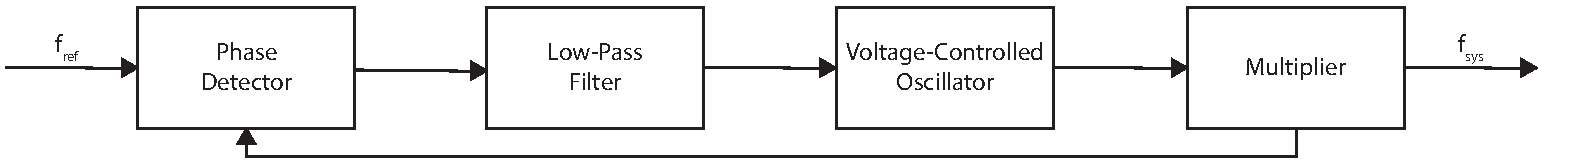
\includegraphics[width=\textwidth]
  {../figure/digital-signal-synthesis/clock-generation.pdf}
  \caption{Clock generation signal generation with \gls{pll} and multiplier.
    The phase detector compares the output system phase with the reference
    phase and yields a non-linear error response. The low-pass filter removes
    fast oscillations. The \gls{vco} changes the output phase in dependence
    of the error response. Finally system and reference phase will go in lock.
    }\label{fig:dds_clock_generation}
\end{figure}
In \Cref{fig:dds_clock_generation} the system clock generation from a
reference signal is illustrated. The phase detector yields a non-linear error
response comparing the output signal phase with the reference signal phase.
After a low-pass filter removes fast oscillations a \gls{vco} changes its
phase proportional to the error signal. Finally a frequency multiplier creates
harmonics of the reference frequency and extracts a programmed frequency
multiple of $M$ such that the system frequency relates to the reference
clock by $f_\text{sys}=Mf_\text{ref}$ with $\mathbb{N}\ni M>1$.

\subsection{Parameter modulation}

So far we only discussed the case of frequency modulation of the generated
output signal, however,wWe will see that it can be easily extended to support
amplitude and phase modulation too.
\begin{figure}[htb]
  \centering
  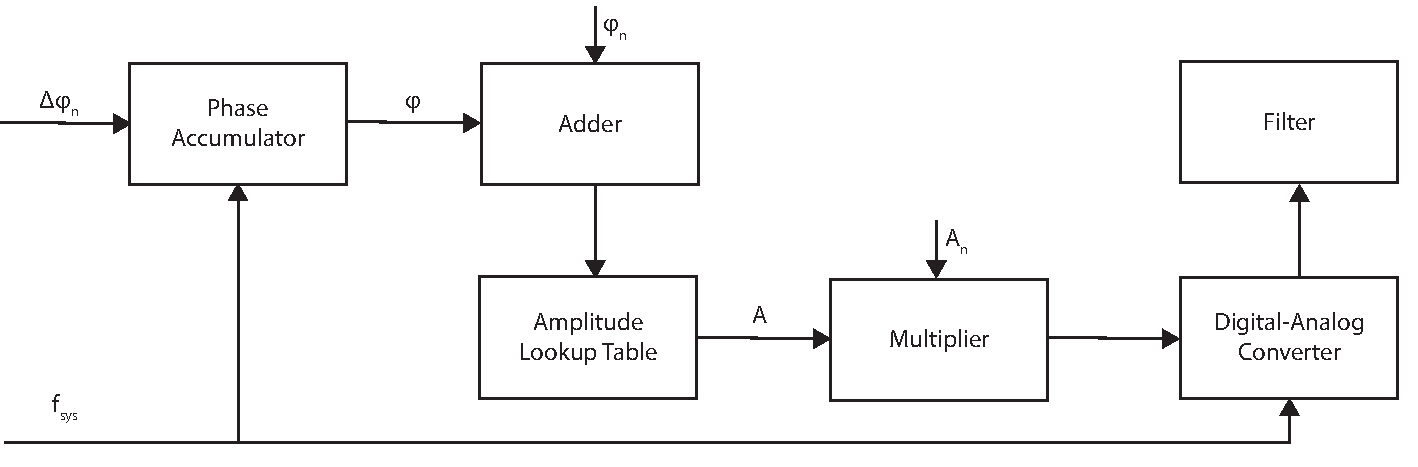
\includegraphics[width=\textwidth]
  {../figure/digital-signal-synthesis/modulation-architecture.pdf}
  \caption{\gls{dds} architecture supporting modulation of frequency,
    amplitude and phase offset parameters. Phase accumulator increment
    $\Delta\varphi(t)$ is now time dependent. The phase offset $\varphi_0(t)$
    is also time dependent and is added as a last step to the phase
    accumulator before supplied to the \gls{dac}. The time dependent amplitude
    parameter $A_n(t)$ is multiplied with the amplitude obtained from the
    lookup table.
  }\label{fig:dds_modulation_architecture}
\end{figure}
In \Cref{fig:dds_modulation_architecture} we can see one realization of an
architecture that supports amplitude, frequency and phase modulation. The main
components are the same as in \Cref{fig:dds_simple_architecture}. In addition
we have an adder for a time dependent phase offset and a multiplier for the
digital amplitude value obtained from the lookup table. The time dependence
of the parameters can be either determined by reading from memory or through
generation of another circuit. In a later section we will discuss the case of
a linear frequency sweep provided by a digital ramp.

\section{Quantization effects}

At the beginning of this chapter we elaborated greatly on the advantages that
digital signal synthesis has to offer. Yet we know that every technical design
involves its unqiue set of compromises. One important part in any engineering
process is to carefully evaluate the implications of these compromises. In
that sense we will discuss the side-effects arising from the digital nature of
digital signal synthesis and what methods there exists to reduce them.

\subsubsection{Phase jitter}

Phase jitter is created when one configures an output frequency for which
$\Delta\varphi$ is not a divider of $2^N$. In this case a phase error builds
up in each clock cycle~\cite{Vankka2013}. According to
\begin{equation}
  \frac{f_\text{out}}{f_\text{sys}}2^N-\Delta\varphi
  \label{eq:dds_phase_error},
\end{equation}
with the phase accumulator increment $\Delta\varphi$ defined in
\cref{eq:dds_phase_increment}, we have a phase error of $.4$ per clock cycle
for the model system parameters listed in \Cref{tab:dds_parameters}. 
\begin{figure}[htb]
  \centering
  \begin{adjustbox}{width=\textwidth}
    %% Creator: Matplotlib, PGF backend
%%
%% To include the figure in your LaTeX document, write
%%   \input{<filename>.pgf}
%%
%% Make sure the required packages are loaded in your preamble
%%   \usepackage{pgf}
%%
%% Figures using additional raster images can only be included by \input if
%% they are in the same directory as the main LaTeX file. For loading figures
%% from other directories you can use the `import` package
%%   \usepackage{import}
%% and then include the figures with
%%   \import{<path to file>}{<filename>.pgf}
%%
%% Matplotlib used the following preamble
%%   \usepackage{amsmath}\usepackage{siunitx}\usepackage{lmodern}
%%   \usepackage{fontspec}
%%
\begingroup%
\makeatletter%
\begin{pgfpicture}%
\pgfpathrectangle{\pgfpointorigin}{\pgfqpoint{12.000000in}{7.000000in}}%
\pgfusepath{use as bounding box, clip}%
\begin{pgfscope}%
\pgfsetbuttcap%
\pgfsetmiterjoin%
\pgfsetlinewidth{0.000000pt}%
\definecolor{currentstroke}{rgb}{1.000000,1.000000,1.000000}%
\pgfsetstrokecolor{currentstroke}%
\pgfsetdash{}{0pt}%
\pgfpathmoveto{\pgfqpoint{0.000000in}{0.000000in}}%
\pgfpathlineto{\pgfqpoint{12.000000in}{0.000000in}}%
\pgfpathlineto{\pgfqpoint{12.000000in}{7.000000in}}%
\pgfpathlineto{\pgfqpoint{0.000000in}{7.000000in}}%
\pgfpathclose%
\pgfusepath{}%
\end{pgfscope}%
\begin{pgfscope}%
\pgfsetbuttcap%
\pgfsetmiterjoin%
\definecolor{currentfill}{rgb}{1.000000,1.000000,1.000000}%
\pgfsetfillcolor{currentfill}%
\pgfsetlinewidth{0.000000pt}%
\definecolor{currentstroke}{rgb}{0.000000,0.000000,0.000000}%
\pgfsetstrokecolor{currentstroke}%
\pgfsetstrokeopacity{0.000000}%
\pgfsetdash{}{0pt}%
\pgfpathmoveto{\pgfqpoint{1.500000in}{4.701290in}}%
\pgfpathlineto{\pgfqpoint{10.800000in}{4.701290in}}%
\pgfpathlineto{\pgfqpoint{10.800000in}{6.440000in}}%
\pgfpathlineto{\pgfqpoint{1.500000in}{6.440000in}}%
\pgfpathclose%
\pgfusepath{fill}%
\end{pgfscope}%
\begin{pgfscope}%
\pgfpathrectangle{\pgfqpoint{1.500000in}{4.701290in}}{\pgfqpoint{9.300000in}{1.738710in}}%
\pgfusepath{clip}%
\pgfsetbuttcap%
\pgfsetroundjoin%
\definecolor{currentfill}{rgb}{0.192157,0.509804,0.741176}%
\pgfsetfillcolor{currentfill}%
\pgfsetlinewidth{1.003750pt}%
\definecolor{currentstroke}{rgb}{0.192157,0.509804,0.741176}%
\pgfsetstrokecolor{currentstroke}%
\pgfsetdash{}{0pt}%
\pgfpathmoveto{\pgfqpoint{1.922812in}{4.758853in}}%
\pgfpathcurveto{\pgfqpoint{1.930178in}{4.758853in}}{\pgfqpoint{1.937245in}{4.761780in}}{\pgfqpoint{1.942454in}{4.766989in}}%
\pgfpathcurveto{\pgfqpoint{1.947663in}{4.772198in}}{\pgfqpoint{1.950590in}{4.779264in}}{\pgfqpoint{1.950590in}{4.786631in}}%
\pgfpathcurveto{\pgfqpoint{1.950590in}{4.793998in}}{\pgfqpoint{1.947663in}{4.801064in}}{\pgfqpoint{1.942454in}{4.806273in}}%
\pgfpathcurveto{\pgfqpoint{1.937245in}{4.811482in}}{\pgfqpoint{1.930178in}{4.814409in}}{\pgfqpoint{1.922812in}{4.814409in}}%
\pgfpathcurveto{\pgfqpoint{1.915445in}{4.814409in}}{\pgfqpoint{1.908379in}{4.811482in}}{\pgfqpoint{1.903170in}{4.806273in}}%
\pgfpathcurveto{\pgfqpoint{1.897961in}{4.801064in}}{\pgfqpoint{1.895034in}{4.793998in}}{\pgfqpoint{1.895034in}{4.786631in}}%
\pgfpathcurveto{\pgfqpoint{1.895034in}{4.779264in}}{\pgfqpoint{1.897961in}{4.772198in}}{\pgfqpoint{1.903170in}{4.766989in}}%
\pgfpathcurveto{\pgfqpoint{1.908379in}{4.761780in}}{\pgfqpoint{1.915445in}{4.758853in}}{\pgfqpoint{1.922812in}{4.758853in}}%
\pgfpathclose%
\pgfusepath{stroke,fill}%
\end{pgfscope}%
\begin{pgfscope}%
\pgfpathrectangle{\pgfqpoint{1.500000in}{4.701290in}}{\pgfqpoint{9.300000in}{1.738710in}}%
\pgfusepath{clip}%
\pgfsetbuttcap%
\pgfsetroundjoin%
\definecolor{currentfill}{rgb}{0.192157,0.509804,0.741176}%
\pgfsetfillcolor{currentfill}%
\pgfsetlinewidth{1.003750pt}%
\definecolor{currentstroke}{rgb}{0.192157,0.509804,0.741176}%
\pgfsetstrokecolor{currentstroke}%
\pgfsetdash{}{0pt}%
\pgfpathmoveto{\pgfqpoint{1.951087in}{4.765051in}}%
\pgfpathcurveto{\pgfqpoint{1.958454in}{4.765051in}}{\pgfqpoint{1.965520in}{4.767978in}}{\pgfqpoint{1.970729in}{4.773187in}}%
\pgfpathcurveto{\pgfqpoint{1.975938in}{4.778396in}}{\pgfqpoint{1.978865in}{4.785462in}}{\pgfqpoint{1.978865in}{4.792829in}}%
\pgfpathcurveto{\pgfqpoint{1.978865in}{4.800196in}}{\pgfqpoint{1.975938in}{4.807262in}}{\pgfqpoint{1.970729in}{4.812471in}}%
\pgfpathcurveto{\pgfqpoint{1.965520in}{4.817680in}}{\pgfqpoint{1.958454in}{4.820607in}}{\pgfqpoint{1.951087in}{4.820607in}}%
\pgfpathcurveto{\pgfqpoint{1.943720in}{4.820607in}}{\pgfqpoint{1.936654in}{4.817680in}}{\pgfqpoint{1.931445in}{4.812471in}}%
\pgfpathcurveto{\pgfqpoint{1.926236in}{4.807262in}}{\pgfqpoint{1.923309in}{4.800196in}}{\pgfqpoint{1.923309in}{4.792829in}}%
\pgfpathcurveto{\pgfqpoint{1.923309in}{4.785462in}}{\pgfqpoint{1.926236in}{4.778396in}}{\pgfqpoint{1.931445in}{4.773187in}}%
\pgfpathcurveto{\pgfqpoint{1.936654in}{4.767978in}}{\pgfqpoint{1.943720in}{4.765051in}}{\pgfqpoint{1.951087in}{4.765051in}}%
\pgfpathclose%
\pgfusepath{stroke,fill}%
\end{pgfscope}%
\begin{pgfscope}%
\pgfpathrectangle{\pgfqpoint{1.500000in}{4.701290in}}{\pgfqpoint{9.300000in}{1.738710in}}%
\pgfusepath{clip}%
\pgfsetbuttcap%
\pgfsetroundjoin%
\definecolor{currentfill}{rgb}{0.192157,0.509804,0.741176}%
\pgfsetfillcolor{currentfill}%
\pgfsetlinewidth{1.003750pt}%
\definecolor{currentstroke}{rgb}{0.192157,0.509804,0.741176}%
\pgfsetstrokecolor{currentstroke}%
\pgfsetdash{}{0pt}%
\pgfpathmoveto{\pgfqpoint{1.979363in}{4.771249in}}%
\pgfpathcurveto{\pgfqpoint{1.986729in}{4.771249in}}{\pgfqpoint{1.993796in}{4.774176in}}{\pgfqpoint{1.999005in}{4.779385in}}%
\pgfpathcurveto{\pgfqpoint{2.004214in}{4.784594in}}{\pgfqpoint{2.007141in}{4.791660in}}{\pgfqpoint{2.007141in}{4.799027in}}%
\pgfpathcurveto{\pgfqpoint{2.007141in}{4.806393in}}{\pgfqpoint{2.004214in}{4.813459in}}{\pgfqpoint{1.999005in}{4.818668in}}%
\pgfpathcurveto{\pgfqpoint{1.993796in}{4.823877in}}{\pgfqpoint{1.986729in}{4.826804in}}{\pgfqpoint{1.979363in}{4.826804in}}%
\pgfpathcurveto{\pgfqpoint{1.971996in}{4.826804in}}{\pgfqpoint{1.964930in}{4.823877in}}{\pgfqpoint{1.959721in}{4.818668in}}%
\pgfpathcurveto{\pgfqpoint{1.954512in}{4.813459in}}{\pgfqpoint{1.951585in}{4.806393in}}{\pgfqpoint{1.951585in}{4.799027in}}%
\pgfpathcurveto{\pgfqpoint{1.951585in}{4.791660in}}{\pgfqpoint{1.954512in}{4.784594in}}{\pgfqpoint{1.959721in}{4.779385in}}%
\pgfpathcurveto{\pgfqpoint{1.964930in}{4.774176in}}{\pgfqpoint{1.971996in}{4.771249in}}{\pgfqpoint{1.979363in}{4.771249in}}%
\pgfpathclose%
\pgfusepath{stroke,fill}%
\end{pgfscope}%
\begin{pgfscope}%
\pgfpathrectangle{\pgfqpoint{1.500000in}{4.701290in}}{\pgfqpoint{9.300000in}{1.738710in}}%
\pgfusepath{clip}%
\pgfsetbuttcap%
\pgfsetroundjoin%
\definecolor{currentfill}{rgb}{0.192157,0.509804,0.741176}%
\pgfsetfillcolor{currentfill}%
\pgfsetlinewidth{1.003750pt}%
\definecolor{currentstroke}{rgb}{0.192157,0.509804,0.741176}%
\pgfsetstrokecolor{currentstroke}%
\pgfsetdash{}{0pt}%
\pgfpathmoveto{\pgfqpoint{2.007638in}{4.777447in}}%
\pgfpathcurveto{\pgfqpoint{2.015005in}{4.777447in}}{\pgfqpoint{2.022071in}{4.780373in}}{\pgfqpoint{2.027280in}{4.785582in}}%
\pgfpathcurveto{\pgfqpoint{2.032489in}{4.790792in}}{\pgfqpoint{2.035416in}{4.797858in}}{\pgfqpoint{2.035416in}{4.805224in}}%
\pgfpathcurveto{\pgfqpoint{2.035416in}{4.812591in}}{\pgfqpoint{2.032489in}{4.819657in}}{\pgfqpoint{2.027280in}{4.824866in}}%
\pgfpathcurveto{\pgfqpoint{2.022071in}{4.830075in}}{\pgfqpoint{2.015005in}{4.833002in}}{\pgfqpoint{2.007638in}{4.833002in}}%
\pgfpathcurveto{\pgfqpoint{2.000271in}{4.833002in}}{\pgfqpoint{1.993205in}{4.830075in}}{\pgfqpoint{1.987996in}{4.824866in}}%
\pgfpathcurveto{\pgfqpoint{1.982787in}{4.819657in}}{\pgfqpoint{1.979860in}{4.812591in}}{\pgfqpoint{1.979860in}{4.805224in}}%
\pgfpathcurveto{\pgfqpoint{1.979860in}{4.797858in}}{\pgfqpoint{1.982787in}{4.790792in}}{\pgfqpoint{1.987996in}{4.785582in}}%
\pgfpathcurveto{\pgfqpoint{1.993205in}{4.780373in}}{\pgfqpoint{2.000271in}{4.777447in}}{\pgfqpoint{2.007638in}{4.777447in}}%
\pgfpathclose%
\pgfusepath{stroke,fill}%
\end{pgfscope}%
\begin{pgfscope}%
\pgfpathrectangle{\pgfqpoint{1.500000in}{4.701290in}}{\pgfqpoint{9.300000in}{1.738710in}}%
\pgfusepath{clip}%
\pgfsetbuttcap%
\pgfsetroundjoin%
\definecolor{currentfill}{rgb}{0.192157,0.509804,0.741176}%
\pgfsetfillcolor{currentfill}%
\pgfsetlinewidth{1.003750pt}%
\definecolor{currentstroke}{rgb}{0.192157,0.509804,0.741176}%
\pgfsetstrokecolor{currentstroke}%
\pgfsetdash{}{0pt}%
\pgfpathmoveto{\pgfqpoint{2.035914in}{4.783644in}}%
\pgfpathcurveto{\pgfqpoint{2.043281in}{4.783644in}}{\pgfqpoint{2.050347in}{4.786571in}}{\pgfqpoint{2.055556in}{4.791780in}}%
\pgfpathcurveto{\pgfqpoint{2.060765in}{4.796989in}}{\pgfqpoint{2.063692in}{4.804055in}}{\pgfqpoint{2.063692in}{4.811422in}}%
\pgfpathcurveto{\pgfqpoint{2.063692in}{4.818789in}}{\pgfqpoint{2.060765in}{4.825855in}}{\pgfqpoint{2.055556in}{4.831064in}}%
\pgfpathcurveto{\pgfqpoint{2.050347in}{4.836273in}}{\pgfqpoint{2.043281in}{4.839200in}}{\pgfqpoint{2.035914in}{4.839200in}}%
\pgfpathcurveto{\pgfqpoint{2.028547in}{4.839200in}}{\pgfqpoint{2.021481in}{4.836273in}}{\pgfqpoint{2.016272in}{4.831064in}}%
\pgfpathcurveto{\pgfqpoint{2.011063in}{4.825855in}}{\pgfqpoint{2.008136in}{4.818789in}}{\pgfqpoint{2.008136in}{4.811422in}}%
\pgfpathcurveto{\pgfqpoint{2.008136in}{4.804055in}}{\pgfqpoint{2.011063in}{4.796989in}}{\pgfqpoint{2.016272in}{4.791780in}}%
\pgfpathcurveto{\pgfqpoint{2.021481in}{4.786571in}}{\pgfqpoint{2.028547in}{4.783644in}}{\pgfqpoint{2.035914in}{4.783644in}}%
\pgfpathclose%
\pgfusepath{stroke,fill}%
\end{pgfscope}%
\begin{pgfscope}%
\pgfpathrectangle{\pgfqpoint{1.500000in}{4.701290in}}{\pgfqpoint{9.300000in}{1.738710in}}%
\pgfusepath{clip}%
\pgfsetbuttcap%
\pgfsetroundjoin%
\definecolor{currentfill}{rgb}{0.192157,0.509804,0.741176}%
\pgfsetfillcolor{currentfill}%
\pgfsetlinewidth{1.003750pt}%
\definecolor{currentstroke}{rgb}{0.192157,0.509804,0.741176}%
\pgfsetstrokecolor{currentstroke}%
\pgfsetdash{}{0pt}%
\pgfpathmoveto{\pgfqpoint{2.064189in}{4.789842in}}%
\pgfpathcurveto{\pgfqpoint{2.071556in}{4.789842in}}{\pgfqpoint{2.078622in}{4.792769in}}{\pgfqpoint{2.083831in}{4.797978in}}%
\pgfpathcurveto{\pgfqpoint{2.089040in}{4.803187in}}{\pgfqpoint{2.091967in}{4.810253in}}{\pgfqpoint{2.091967in}{4.817620in}}%
\pgfpathcurveto{\pgfqpoint{2.091967in}{4.824987in}}{\pgfqpoint{2.089040in}{4.832053in}}{\pgfqpoint{2.083831in}{4.837262in}}%
\pgfpathcurveto{\pgfqpoint{2.078622in}{4.842471in}}{\pgfqpoint{2.071556in}{4.845398in}}{\pgfqpoint{2.064189in}{4.845398in}}%
\pgfpathcurveto{\pgfqpoint{2.056823in}{4.845398in}}{\pgfqpoint{2.049756in}{4.842471in}}{\pgfqpoint{2.044547in}{4.837262in}}%
\pgfpathcurveto{\pgfqpoint{2.039338in}{4.832053in}}{\pgfqpoint{2.036411in}{4.824987in}}{\pgfqpoint{2.036411in}{4.817620in}}%
\pgfpathcurveto{\pgfqpoint{2.036411in}{4.810253in}}{\pgfqpoint{2.039338in}{4.803187in}}{\pgfqpoint{2.044547in}{4.797978in}}%
\pgfpathcurveto{\pgfqpoint{2.049756in}{4.792769in}}{\pgfqpoint{2.056823in}{4.789842in}}{\pgfqpoint{2.064189in}{4.789842in}}%
\pgfpathclose%
\pgfusepath{stroke,fill}%
\end{pgfscope}%
\begin{pgfscope}%
\pgfpathrectangle{\pgfqpoint{1.500000in}{4.701290in}}{\pgfqpoint{9.300000in}{1.738710in}}%
\pgfusepath{clip}%
\pgfsetbuttcap%
\pgfsetroundjoin%
\definecolor{currentfill}{rgb}{0.192157,0.509804,0.741176}%
\pgfsetfillcolor{currentfill}%
\pgfsetlinewidth{1.003750pt}%
\definecolor{currentstroke}{rgb}{0.192157,0.509804,0.741176}%
\pgfsetstrokecolor{currentstroke}%
\pgfsetdash{}{0pt}%
\pgfpathmoveto{\pgfqpoint{2.092465in}{4.796040in}}%
\pgfpathcurveto{\pgfqpoint{2.099832in}{4.796040in}}{\pgfqpoint{2.106898in}{4.798967in}}{\pgfqpoint{2.112107in}{4.804176in}}%
\pgfpathcurveto{\pgfqpoint{2.117316in}{4.809385in}}{\pgfqpoint{2.120243in}{4.816451in}}{\pgfqpoint{2.120243in}{4.823818in}}%
\pgfpathcurveto{\pgfqpoint{2.120243in}{4.831184in}}{\pgfqpoint{2.117316in}{4.838250in}}{\pgfqpoint{2.112107in}{4.843459in}}%
\pgfpathcurveto{\pgfqpoint{2.106898in}{4.848668in}}{\pgfqpoint{2.099832in}{4.851595in}}{\pgfqpoint{2.092465in}{4.851595in}}%
\pgfpathcurveto{\pgfqpoint{2.085098in}{4.851595in}}{\pgfqpoint{2.078032in}{4.848668in}}{\pgfqpoint{2.072823in}{4.843459in}}%
\pgfpathcurveto{\pgfqpoint{2.067614in}{4.838250in}}{\pgfqpoint{2.064687in}{4.831184in}}{\pgfqpoint{2.064687in}{4.823818in}}%
\pgfpathcurveto{\pgfqpoint{2.064687in}{4.816451in}}{\pgfqpoint{2.067614in}{4.809385in}}{\pgfqpoint{2.072823in}{4.804176in}}%
\pgfpathcurveto{\pgfqpoint{2.078032in}{4.798967in}}{\pgfqpoint{2.085098in}{4.796040in}}{\pgfqpoint{2.092465in}{4.796040in}}%
\pgfpathclose%
\pgfusepath{stroke,fill}%
\end{pgfscope}%
\begin{pgfscope}%
\pgfpathrectangle{\pgfqpoint{1.500000in}{4.701290in}}{\pgfqpoint{9.300000in}{1.738710in}}%
\pgfusepath{clip}%
\pgfsetbuttcap%
\pgfsetroundjoin%
\definecolor{currentfill}{rgb}{0.192157,0.509804,0.741176}%
\pgfsetfillcolor{currentfill}%
\pgfsetlinewidth{1.003750pt}%
\definecolor{currentstroke}{rgb}{0.192157,0.509804,0.741176}%
\pgfsetstrokecolor{currentstroke}%
\pgfsetdash{}{0pt}%
\pgfpathmoveto{\pgfqpoint{2.120740in}{4.802237in}}%
\pgfpathcurveto{\pgfqpoint{2.128107in}{4.802237in}}{\pgfqpoint{2.135173in}{4.805164in}}{\pgfqpoint{2.140382in}{4.810373in}}%
\pgfpathcurveto{\pgfqpoint{2.145591in}{4.815582in}}{\pgfqpoint{2.148518in}{4.822649in}}{\pgfqpoint{2.148518in}{4.830015in}}%
\pgfpathcurveto{\pgfqpoint{2.148518in}{4.837382in}}{\pgfqpoint{2.145591in}{4.844448in}}{\pgfqpoint{2.140382in}{4.849657in}}%
\pgfpathcurveto{\pgfqpoint{2.135173in}{4.854866in}}{\pgfqpoint{2.128107in}{4.857793in}}{\pgfqpoint{2.120740in}{4.857793in}}%
\pgfpathcurveto{\pgfqpoint{2.113374in}{4.857793in}}{\pgfqpoint{2.106308in}{4.854866in}}{\pgfqpoint{2.101098in}{4.849657in}}%
\pgfpathcurveto{\pgfqpoint{2.095889in}{4.844448in}}{\pgfqpoint{2.092962in}{4.837382in}}{\pgfqpoint{2.092962in}{4.830015in}}%
\pgfpathcurveto{\pgfqpoint{2.092962in}{4.822649in}}{\pgfqpoint{2.095889in}{4.815582in}}{\pgfqpoint{2.101098in}{4.810373in}}%
\pgfpathcurveto{\pgfqpoint{2.106308in}{4.805164in}}{\pgfqpoint{2.113374in}{4.802237in}}{\pgfqpoint{2.120740in}{4.802237in}}%
\pgfpathclose%
\pgfusepath{stroke,fill}%
\end{pgfscope}%
\begin{pgfscope}%
\pgfpathrectangle{\pgfqpoint{1.500000in}{4.701290in}}{\pgfqpoint{9.300000in}{1.738710in}}%
\pgfusepath{clip}%
\pgfsetbuttcap%
\pgfsetroundjoin%
\definecolor{currentfill}{rgb}{0.192157,0.509804,0.741176}%
\pgfsetfillcolor{currentfill}%
\pgfsetlinewidth{1.003750pt}%
\definecolor{currentstroke}{rgb}{0.192157,0.509804,0.741176}%
\pgfsetstrokecolor{currentstroke}%
\pgfsetdash{}{0pt}%
\pgfpathmoveto{\pgfqpoint{2.149016in}{4.808435in}}%
\pgfpathcurveto{\pgfqpoint{2.156383in}{4.808435in}}{\pgfqpoint{2.163449in}{4.811362in}}{\pgfqpoint{2.168658in}{4.816571in}}%
\pgfpathcurveto{\pgfqpoint{2.173867in}{4.821780in}}{\pgfqpoint{2.176794in}{4.828846in}}{\pgfqpoint{2.176794in}{4.836213in}}%
\pgfpathcurveto{\pgfqpoint{2.176794in}{4.843580in}}{\pgfqpoint{2.173867in}{4.850646in}}{\pgfqpoint{2.168658in}{4.855855in}}%
\pgfpathcurveto{\pgfqpoint{2.163449in}{4.861064in}}{\pgfqpoint{2.156383in}{4.863991in}}{\pgfqpoint{2.149016in}{4.863991in}}%
\pgfpathcurveto{\pgfqpoint{2.141649in}{4.863991in}}{\pgfqpoint{2.134583in}{4.861064in}}{\pgfqpoint{2.129374in}{4.855855in}}%
\pgfpathcurveto{\pgfqpoint{2.124165in}{4.850646in}}{\pgfqpoint{2.121238in}{4.843580in}}{\pgfqpoint{2.121238in}{4.836213in}}%
\pgfpathcurveto{\pgfqpoint{2.121238in}{4.828846in}}{\pgfqpoint{2.124165in}{4.821780in}}{\pgfqpoint{2.129374in}{4.816571in}}%
\pgfpathcurveto{\pgfqpoint{2.134583in}{4.811362in}}{\pgfqpoint{2.141649in}{4.808435in}}{\pgfqpoint{2.149016in}{4.808435in}}%
\pgfpathclose%
\pgfusepath{stroke,fill}%
\end{pgfscope}%
\begin{pgfscope}%
\pgfpathrectangle{\pgfqpoint{1.500000in}{4.701290in}}{\pgfqpoint{9.300000in}{1.738710in}}%
\pgfusepath{clip}%
\pgfsetbuttcap%
\pgfsetroundjoin%
\definecolor{currentfill}{rgb}{0.192157,0.509804,0.741176}%
\pgfsetfillcolor{currentfill}%
\pgfsetlinewidth{1.003750pt}%
\definecolor{currentstroke}{rgb}{0.192157,0.509804,0.741176}%
\pgfsetstrokecolor{currentstroke}%
\pgfsetdash{}{0pt}%
\pgfpathmoveto{\pgfqpoint{2.177291in}{4.814633in}}%
\pgfpathcurveto{\pgfqpoint{2.184658in}{4.814633in}}{\pgfqpoint{2.191724in}{4.817560in}}{\pgfqpoint{2.196933in}{4.822769in}}%
\pgfpathcurveto{\pgfqpoint{2.202142in}{4.827978in}}{\pgfqpoint{2.205069in}{4.835044in}}{\pgfqpoint{2.205069in}{4.842411in}}%
\pgfpathcurveto{\pgfqpoint{2.205069in}{4.849777in}}{\pgfqpoint{2.202142in}{4.856844in}}{\pgfqpoint{2.196933in}{4.862053in}}%
\pgfpathcurveto{\pgfqpoint{2.191724in}{4.867262in}}{\pgfqpoint{2.184658in}{4.870189in}}{\pgfqpoint{2.177291in}{4.870189in}}%
\pgfpathcurveto{\pgfqpoint{2.169925in}{4.870189in}}{\pgfqpoint{2.162859in}{4.867262in}}{\pgfqpoint{2.157649in}{4.862053in}}%
\pgfpathcurveto{\pgfqpoint{2.152440in}{4.856844in}}{\pgfqpoint{2.149514in}{4.849777in}}{\pgfqpoint{2.149514in}{4.842411in}}%
\pgfpathcurveto{\pgfqpoint{2.149514in}{4.835044in}}{\pgfqpoint{2.152440in}{4.827978in}}{\pgfqpoint{2.157649in}{4.822769in}}%
\pgfpathcurveto{\pgfqpoint{2.162859in}{4.817560in}}{\pgfqpoint{2.169925in}{4.814633in}}{\pgfqpoint{2.177291in}{4.814633in}}%
\pgfpathclose%
\pgfusepath{stroke,fill}%
\end{pgfscope}%
\begin{pgfscope}%
\pgfpathrectangle{\pgfqpoint{1.500000in}{4.701290in}}{\pgfqpoint{9.300000in}{1.738710in}}%
\pgfusepath{clip}%
\pgfsetbuttcap%
\pgfsetroundjoin%
\definecolor{currentfill}{rgb}{0.192157,0.509804,0.741176}%
\pgfsetfillcolor{currentfill}%
\pgfsetlinewidth{1.003750pt}%
\definecolor{currentstroke}{rgb}{0.192157,0.509804,0.741176}%
\pgfsetstrokecolor{currentstroke}%
\pgfsetdash{}{0pt}%
\pgfpathmoveto{\pgfqpoint{2.205567in}{4.820831in}}%
\pgfpathcurveto{\pgfqpoint{2.212934in}{4.820831in}}{\pgfqpoint{2.220000in}{4.823758in}}{\pgfqpoint{2.225209in}{4.828967in}}%
\pgfpathcurveto{\pgfqpoint{2.230418in}{4.834176in}}{\pgfqpoint{2.233345in}{4.841242in}}{\pgfqpoint{2.233345in}{4.848608in}}%
\pgfpathcurveto{\pgfqpoint{2.233345in}{4.855975in}}{\pgfqpoint{2.230418in}{4.863041in}}{\pgfqpoint{2.225209in}{4.868250in}}%
\pgfpathcurveto{\pgfqpoint{2.220000in}{4.873459in}}{\pgfqpoint{2.212934in}{4.876386in}}{\pgfqpoint{2.205567in}{4.876386in}}%
\pgfpathcurveto{\pgfqpoint{2.198200in}{4.876386in}}{\pgfqpoint{2.191134in}{4.873459in}}{\pgfqpoint{2.185925in}{4.868250in}}%
\pgfpathcurveto{\pgfqpoint{2.180716in}{4.863041in}}{\pgfqpoint{2.177789in}{4.855975in}}{\pgfqpoint{2.177789in}{4.848608in}}%
\pgfpathcurveto{\pgfqpoint{2.177789in}{4.841242in}}{\pgfqpoint{2.180716in}{4.834176in}}{\pgfqpoint{2.185925in}{4.828967in}}%
\pgfpathcurveto{\pgfqpoint{2.191134in}{4.823758in}}{\pgfqpoint{2.198200in}{4.820831in}}{\pgfqpoint{2.205567in}{4.820831in}}%
\pgfpathclose%
\pgfusepath{stroke,fill}%
\end{pgfscope}%
\begin{pgfscope}%
\pgfpathrectangle{\pgfqpoint{1.500000in}{4.701290in}}{\pgfqpoint{9.300000in}{1.738710in}}%
\pgfusepath{clip}%
\pgfsetbuttcap%
\pgfsetroundjoin%
\definecolor{currentfill}{rgb}{0.192157,0.509804,0.741176}%
\pgfsetfillcolor{currentfill}%
\pgfsetlinewidth{1.003750pt}%
\definecolor{currentstroke}{rgb}{0.192157,0.509804,0.741176}%
\pgfsetstrokecolor{currentstroke}%
\pgfsetdash{}{0pt}%
\pgfpathmoveto{\pgfqpoint{2.233842in}{4.827028in}}%
\pgfpathcurveto{\pgfqpoint{2.241209in}{4.827028in}}{\pgfqpoint{2.248275in}{4.829955in}}{\pgfqpoint{2.253484in}{4.835164in}}%
\pgfpathcurveto{\pgfqpoint{2.258693in}{4.840373in}}{\pgfqpoint{2.261620in}{4.847439in}}{\pgfqpoint{2.261620in}{4.854806in}}%
\pgfpathcurveto{\pgfqpoint{2.261620in}{4.862173in}}{\pgfqpoint{2.258693in}{4.869239in}}{\pgfqpoint{2.253484in}{4.874448in}}%
\pgfpathcurveto{\pgfqpoint{2.248275in}{4.879657in}}{\pgfqpoint{2.241209in}{4.882584in}}{\pgfqpoint{2.233842in}{4.882584in}}%
\pgfpathcurveto{\pgfqpoint{2.226476in}{4.882584in}}{\pgfqpoint{2.219410in}{4.879657in}}{\pgfqpoint{2.214200in}{4.874448in}}%
\pgfpathcurveto{\pgfqpoint{2.208991in}{4.869239in}}{\pgfqpoint{2.206065in}{4.862173in}}{\pgfqpoint{2.206065in}{4.854806in}}%
\pgfpathcurveto{\pgfqpoint{2.206065in}{4.847439in}}{\pgfqpoint{2.208991in}{4.840373in}}{\pgfqpoint{2.214200in}{4.835164in}}%
\pgfpathcurveto{\pgfqpoint{2.219410in}{4.829955in}}{\pgfqpoint{2.226476in}{4.827028in}}{\pgfqpoint{2.233842in}{4.827028in}}%
\pgfpathclose%
\pgfusepath{stroke,fill}%
\end{pgfscope}%
\begin{pgfscope}%
\pgfpathrectangle{\pgfqpoint{1.500000in}{4.701290in}}{\pgfqpoint{9.300000in}{1.738710in}}%
\pgfusepath{clip}%
\pgfsetbuttcap%
\pgfsetroundjoin%
\definecolor{currentfill}{rgb}{0.192157,0.509804,0.741176}%
\pgfsetfillcolor{currentfill}%
\pgfsetlinewidth{1.003750pt}%
\definecolor{currentstroke}{rgb}{0.192157,0.509804,0.741176}%
\pgfsetstrokecolor{currentstroke}%
\pgfsetdash{}{0pt}%
\pgfpathmoveto{\pgfqpoint{2.262118in}{4.833226in}}%
\pgfpathcurveto{\pgfqpoint{2.269485in}{4.833226in}}{\pgfqpoint{2.276551in}{4.836153in}}{\pgfqpoint{2.281760in}{4.841362in}}%
\pgfpathcurveto{\pgfqpoint{2.286969in}{4.846571in}}{\pgfqpoint{2.289896in}{4.853637in}}{\pgfqpoint{2.289896in}{4.861004in}}%
\pgfpathcurveto{\pgfqpoint{2.289896in}{4.868371in}}{\pgfqpoint{2.286969in}{4.875437in}}{\pgfqpoint{2.281760in}{4.880646in}}%
\pgfpathcurveto{\pgfqpoint{2.276551in}{4.885855in}}{\pgfqpoint{2.269485in}{4.888782in}}{\pgfqpoint{2.262118in}{4.888782in}}%
\pgfpathcurveto{\pgfqpoint{2.254751in}{4.888782in}}{\pgfqpoint{2.247685in}{4.885855in}}{\pgfqpoint{2.242476in}{4.880646in}}%
\pgfpathcurveto{\pgfqpoint{2.237267in}{4.875437in}}{\pgfqpoint{2.234340in}{4.868371in}}{\pgfqpoint{2.234340in}{4.861004in}}%
\pgfpathcurveto{\pgfqpoint{2.234340in}{4.853637in}}{\pgfqpoint{2.237267in}{4.846571in}}{\pgfqpoint{2.242476in}{4.841362in}}%
\pgfpathcurveto{\pgfqpoint{2.247685in}{4.836153in}}{\pgfqpoint{2.254751in}{4.833226in}}{\pgfqpoint{2.262118in}{4.833226in}}%
\pgfpathclose%
\pgfusepath{stroke,fill}%
\end{pgfscope}%
\begin{pgfscope}%
\pgfpathrectangle{\pgfqpoint{1.500000in}{4.701290in}}{\pgfqpoint{9.300000in}{1.738710in}}%
\pgfusepath{clip}%
\pgfsetbuttcap%
\pgfsetroundjoin%
\definecolor{currentfill}{rgb}{0.192157,0.509804,0.741176}%
\pgfsetfillcolor{currentfill}%
\pgfsetlinewidth{1.003750pt}%
\definecolor{currentstroke}{rgb}{0.192157,0.509804,0.741176}%
\pgfsetstrokecolor{currentstroke}%
\pgfsetdash{}{0pt}%
\pgfpathmoveto{\pgfqpoint{2.290393in}{4.839424in}}%
\pgfpathcurveto{\pgfqpoint{2.297760in}{4.839424in}}{\pgfqpoint{2.304826in}{4.842351in}}{\pgfqpoint{2.310035in}{4.847560in}}%
\pgfpathcurveto{\pgfqpoint{2.315244in}{4.852769in}}{\pgfqpoint{2.318171in}{4.859835in}}{\pgfqpoint{2.318171in}{4.867202in}}%
\pgfpathcurveto{\pgfqpoint{2.318171in}{4.874568in}}{\pgfqpoint{2.315244in}{4.881634in}}{\pgfqpoint{2.310035in}{4.886844in}}%
\pgfpathcurveto{\pgfqpoint{2.304826in}{4.892053in}}{\pgfqpoint{2.297760in}{4.894979in}}{\pgfqpoint{2.290393in}{4.894979in}}%
\pgfpathcurveto{\pgfqpoint{2.283027in}{4.894979in}}{\pgfqpoint{2.275961in}{4.892053in}}{\pgfqpoint{2.270751in}{4.886844in}}%
\pgfpathcurveto{\pgfqpoint{2.265542in}{4.881634in}}{\pgfqpoint{2.262616in}{4.874568in}}{\pgfqpoint{2.262616in}{4.867202in}}%
\pgfpathcurveto{\pgfqpoint{2.262616in}{4.859835in}}{\pgfqpoint{2.265542in}{4.852769in}}{\pgfqpoint{2.270751in}{4.847560in}}%
\pgfpathcurveto{\pgfqpoint{2.275961in}{4.842351in}}{\pgfqpoint{2.283027in}{4.839424in}}{\pgfqpoint{2.290393in}{4.839424in}}%
\pgfpathclose%
\pgfusepath{stroke,fill}%
\end{pgfscope}%
\begin{pgfscope}%
\pgfpathrectangle{\pgfqpoint{1.500000in}{4.701290in}}{\pgfqpoint{9.300000in}{1.738710in}}%
\pgfusepath{clip}%
\pgfsetbuttcap%
\pgfsetroundjoin%
\definecolor{currentfill}{rgb}{0.192157,0.509804,0.741176}%
\pgfsetfillcolor{currentfill}%
\pgfsetlinewidth{1.003750pt}%
\definecolor{currentstroke}{rgb}{0.192157,0.509804,0.741176}%
\pgfsetstrokecolor{currentstroke}%
\pgfsetdash{}{0pt}%
\pgfpathmoveto{\pgfqpoint{2.318669in}{4.845622in}}%
\pgfpathcurveto{\pgfqpoint{2.326036in}{4.845622in}}{\pgfqpoint{2.333102in}{4.848548in}}{\pgfqpoint{2.338311in}{4.853758in}}%
\pgfpathcurveto{\pgfqpoint{2.343520in}{4.858967in}}{\pgfqpoint{2.346447in}{4.866033in}}{\pgfqpoint{2.346447in}{4.873399in}}%
\pgfpathcurveto{\pgfqpoint{2.346447in}{4.880766in}}{\pgfqpoint{2.343520in}{4.887832in}}{\pgfqpoint{2.338311in}{4.893041in}}%
\pgfpathcurveto{\pgfqpoint{2.333102in}{4.898250in}}{\pgfqpoint{2.326036in}{4.901177in}}{\pgfqpoint{2.318669in}{4.901177in}}%
\pgfpathcurveto{\pgfqpoint{2.311302in}{4.901177in}}{\pgfqpoint{2.304236in}{4.898250in}}{\pgfqpoint{2.299027in}{4.893041in}}%
\pgfpathcurveto{\pgfqpoint{2.293818in}{4.887832in}}{\pgfqpoint{2.290891in}{4.880766in}}{\pgfqpoint{2.290891in}{4.873399in}}%
\pgfpathcurveto{\pgfqpoint{2.290891in}{4.866033in}}{\pgfqpoint{2.293818in}{4.858967in}}{\pgfqpoint{2.299027in}{4.853758in}}%
\pgfpathcurveto{\pgfqpoint{2.304236in}{4.848548in}}{\pgfqpoint{2.311302in}{4.845622in}}{\pgfqpoint{2.318669in}{4.845622in}}%
\pgfpathclose%
\pgfusepath{stroke,fill}%
\end{pgfscope}%
\begin{pgfscope}%
\pgfpathrectangle{\pgfqpoint{1.500000in}{4.701290in}}{\pgfqpoint{9.300000in}{1.738710in}}%
\pgfusepath{clip}%
\pgfsetbuttcap%
\pgfsetroundjoin%
\definecolor{currentfill}{rgb}{0.192157,0.509804,0.741176}%
\pgfsetfillcolor{currentfill}%
\pgfsetlinewidth{1.003750pt}%
\definecolor{currentstroke}{rgb}{0.192157,0.509804,0.741176}%
\pgfsetstrokecolor{currentstroke}%
\pgfsetdash{}{0pt}%
\pgfpathmoveto{\pgfqpoint{2.346944in}{4.851819in}}%
\pgfpathcurveto{\pgfqpoint{2.354311in}{4.851819in}}{\pgfqpoint{2.361377in}{4.854746in}}{\pgfqpoint{2.366586in}{4.859955in}}%
\pgfpathcurveto{\pgfqpoint{2.371795in}{4.865164in}}{\pgfqpoint{2.374722in}{4.872230in}}{\pgfqpoint{2.374722in}{4.879597in}}%
\pgfpathcurveto{\pgfqpoint{2.374722in}{4.886964in}}{\pgfqpoint{2.371795in}{4.894030in}}{\pgfqpoint{2.366586in}{4.899239in}}%
\pgfpathcurveto{\pgfqpoint{2.361377in}{4.904448in}}{\pgfqpoint{2.354311in}{4.907375in}}{\pgfqpoint{2.346944in}{4.907375in}}%
\pgfpathcurveto{\pgfqpoint{2.339578in}{4.907375in}}{\pgfqpoint{2.332512in}{4.904448in}}{\pgfqpoint{2.327302in}{4.899239in}}%
\pgfpathcurveto{\pgfqpoint{2.322093in}{4.894030in}}{\pgfqpoint{2.319167in}{4.886964in}}{\pgfqpoint{2.319167in}{4.879597in}}%
\pgfpathcurveto{\pgfqpoint{2.319167in}{4.872230in}}{\pgfqpoint{2.322093in}{4.865164in}}{\pgfqpoint{2.327302in}{4.859955in}}%
\pgfpathcurveto{\pgfqpoint{2.332512in}{4.854746in}}{\pgfqpoint{2.339578in}{4.851819in}}{\pgfqpoint{2.346944in}{4.851819in}}%
\pgfpathclose%
\pgfusepath{stroke,fill}%
\end{pgfscope}%
\begin{pgfscope}%
\pgfpathrectangle{\pgfqpoint{1.500000in}{4.701290in}}{\pgfqpoint{9.300000in}{1.738710in}}%
\pgfusepath{clip}%
\pgfsetbuttcap%
\pgfsetroundjoin%
\definecolor{currentfill}{rgb}{0.192157,0.509804,0.741176}%
\pgfsetfillcolor{currentfill}%
\pgfsetlinewidth{1.003750pt}%
\definecolor{currentstroke}{rgb}{0.192157,0.509804,0.741176}%
\pgfsetstrokecolor{currentstroke}%
\pgfsetdash{}{0pt}%
\pgfpathmoveto{\pgfqpoint{2.375220in}{4.858017in}}%
\pgfpathcurveto{\pgfqpoint{2.382587in}{4.858017in}}{\pgfqpoint{2.389653in}{4.860944in}}{\pgfqpoint{2.394862in}{4.866153in}}%
\pgfpathcurveto{\pgfqpoint{2.400071in}{4.871362in}}{\pgfqpoint{2.402998in}{4.878428in}}{\pgfqpoint{2.402998in}{4.885795in}}%
\pgfpathcurveto{\pgfqpoint{2.402998in}{4.893162in}}{\pgfqpoint{2.400071in}{4.900228in}}{\pgfqpoint{2.394862in}{4.905437in}}%
\pgfpathcurveto{\pgfqpoint{2.389653in}{4.910646in}}{\pgfqpoint{2.382587in}{4.913573in}}{\pgfqpoint{2.375220in}{4.913573in}}%
\pgfpathcurveto{\pgfqpoint{2.367853in}{4.913573in}}{\pgfqpoint{2.360787in}{4.910646in}}{\pgfqpoint{2.355578in}{4.905437in}}%
\pgfpathcurveto{\pgfqpoint{2.350369in}{4.900228in}}{\pgfqpoint{2.347442in}{4.893162in}}{\pgfqpoint{2.347442in}{4.885795in}}%
\pgfpathcurveto{\pgfqpoint{2.347442in}{4.878428in}}{\pgfqpoint{2.350369in}{4.871362in}}{\pgfqpoint{2.355578in}{4.866153in}}%
\pgfpathcurveto{\pgfqpoint{2.360787in}{4.860944in}}{\pgfqpoint{2.367853in}{4.858017in}}{\pgfqpoint{2.375220in}{4.858017in}}%
\pgfpathclose%
\pgfusepath{stroke,fill}%
\end{pgfscope}%
\begin{pgfscope}%
\pgfpathrectangle{\pgfqpoint{1.500000in}{4.701290in}}{\pgfqpoint{9.300000in}{1.738710in}}%
\pgfusepath{clip}%
\pgfsetbuttcap%
\pgfsetroundjoin%
\definecolor{currentfill}{rgb}{0.192157,0.509804,0.741176}%
\pgfsetfillcolor{currentfill}%
\pgfsetlinewidth{1.003750pt}%
\definecolor{currentstroke}{rgb}{0.192157,0.509804,0.741176}%
\pgfsetstrokecolor{currentstroke}%
\pgfsetdash{}{0pt}%
\pgfpathmoveto{\pgfqpoint{2.403495in}{4.864215in}}%
\pgfpathcurveto{\pgfqpoint{2.410862in}{4.864215in}}{\pgfqpoint{2.417928in}{4.867142in}}{\pgfqpoint{2.423137in}{4.872351in}}%
\pgfpathcurveto{\pgfqpoint{2.428346in}{4.877560in}}{\pgfqpoint{2.431273in}{4.884626in}}{\pgfqpoint{2.431273in}{4.891993in}}%
\pgfpathcurveto{\pgfqpoint{2.431273in}{4.899359in}}{\pgfqpoint{2.428346in}{4.906425in}}{\pgfqpoint{2.423137in}{4.911635in}}%
\pgfpathcurveto{\pgfqpoint{2.417928in}{4.916844in}}{\pgfqpoint{2.410862in}{4.919770in}}{\pgfqpoint{2.403495in}{4.919770in}}%
\pgfpathcurveto{\pgfqpoint{2.396129in}{4.919770in}}{\pgfqpoint{2.389063in}{4.916844in}}{\pgfqpoint{2.383853in}{4.911635in}}%
\pgfpathcurveto{\pgfqpoint{2.378644in}{4.906425in}}{\pgfqpoint{2.375718in}{4.899359in}}{\pgfqpoint{2.375718in}{4.891993in}}%
\pgfpathcurveto{\pgfqpoint{2.375718in}{4.884626in}}{\pgfqpoint{2.378644in}{4.877560in}}{\pgfqpoint{2.383853in}{4.872351in}}%
\pgfpathcurveto{\pgfqpoint{2.389063in}{4.867142in}}{\pgfqpoint{2.396129in}{4.864215in}}{\pgfqpoint{2.403495in}{4.864215in}}%
\pgfpathclose%
\pgfusepath{stroke,fill}%
\end{pgfscope}%
\begin{pgfscope}%
\pgfpathrectangle{\pgfqpoint{1.500000in}{4.701290in}}{\pgfqpoint{9.300000in}{1.738710in}}%
\pgfusepath{clip}%
\pgfsetbuttcap%
\pgfsetroundjoin%
\definecolor{currentfill}{rgb}{0.192157,0.509804,0.741176}%
\pgfsetfillcolor{currentfill}%
\pgfsetlinewidth{1.003750pt}%
\definecolor{currentstroke}{rgb}{0.192157,0.509804,0.741176}%
\pgfsetstrokecolor{currentstroke}%
\pgfsetdash{}{0pt}%
\pgfpathmoveto{\pgfqpoint{2.431771in}{4.870413in}}%
\pgfpathcurveto{\pgfqpoint{2.439138in}{4.870413in}}{\pgfqpoint{2.446204in}{4.873339in}}{\pgfqpoint{2.451413in}{4.878549in}}%
\pgfpathcurveto{\pgfqpoint{2.456622in}{4.883758in}}{\pgfqpoint{2.459549in}{4.890824in}}{\pgfqpoint{2.459549in}{4.898190in}}%
\pgfpathcurveto{\pgfqpoint{2.459549in}{4.905557in}}{\pgfqpoint{2.456622in}{4.912623in}}{\pgfqpoint{2.451413in}{4.917832in}}%
\pgfpathcurveto{\pgfqpoint{2.446204in}{4.923041in}}{\pgfqpoint{2.439138in}{4.925968in}}{\pgfqpoint{2.431771in}{4.925968in}}%
\pgfpathcurveto{\pgfqpoint{2.424404in}{4.925968in}}{\pgfqpoint{2.417338in}{4.923041in}}{\pgfqpoint{2.412129in}{4.917832in}}%
\pgfpathcurveto{\pgfqpoint{2.406920in}{4.912623in}}{\pgfqpoint{2.403993in}{4.905557in}}{\pgfqpoint{2.403993in}{4.898190in}}%
\pgfpathcurveto{\pgfqpoint{2.403993in}{4.890824in}}{\pgfqpoint{2.406920in}{4.883758in}}{\pgfqpoint{2.412129in}{4.878549in}}%
\pgfpathcurveto{\pgfqpoint{2.417338in}{4.873339in}}{\pgfqpoint{2.424404in}{4.870413in}}{\pgfqpoint{2.431771in}{4.870413in}}%
\pgfpathclose%
\pgfusepath{stroke,fill}%
\end{pgfscope}%
\begin{pgfscope}%
\pgfpathrectangle{\pgfqpoint{1.500000in}{4.701290in}}{\pgfqpoint{9.300000in}{1.738710in}}%
\pgfusepath{clip}%
\pgfsetbuttcap%
\pgfsetroundjoin%
\definecolor{currentfill}{rgb}{0.192157,0.509804,0.741176}%
\pgfsetfillcolor{currentfill}%
\pgfsetlinewidth{1.003750pt}%
\definecolor{currentstroke}{rgb}{0.192157,0.509804,0.741176}%
\pgfsetstrokecolor{currentstroke}%
\pgfsetdash{}{0pt}%
\pgfpathmoveto{\pgfqpoint{2.460046in}{4.876610in}}%
\pgfpathcurveto{\pgfqpoint{2.467413in}{4.876610in}}{\pgfqpoint{2.474479in}{4.879537in}}{\pgfqpoint{2.479688in}{4.884746in}}%
\pgfpathcurveto{\pgfqpoint{2.484897in}{4.889955in}}{\pgfqpoint{2.487824in}{4.897021in}}{\pgfqpoint{2.487824in}{4.904388in}}%
\pgfpathcurveto{\pgfqpoint{2.487824in}{4.911755in}}{\pgfqpoint{2.484897in}{4.918821in}}{\pgfqpoint{2.479688in}{4.924030in}}%
\pgfpathcurveto{\pgfqpoint{2.474479in}{4.929239in}}{\pgfqpoint{2.467413in}{4.932166in}}{\pgfqpoint{2.460046in}{4.932166in}}%
\pgfpathcurveto{\pgfqpoint{2.452680in}{4.932166in}}{\pgfqpoint{2.445614in}{4.929239in}}{\pgfqpoint{2.440405in}{4.924030in}}%
\pgfpathcurveto{\pgfqpoint{2.435195in}{4.918821in}}{\pgfqpoint{2.432269in}{4.911755in}}{\pgfqpoint{2.432269in}{4.904388in}}%
\pgfpathcurveto{\pgfqpoint{2.432269in}{4.897021in}}{\pgfqpoint{2.435195in}{4.889955in}}{\pgfqpoint{2.440405in}{4.884746in}}%
\pgfpathcurveto{\pgfqpoint{2.445614in}{4.879537in}}{\pgfqpoint{2.452680in}{4.876610in}}{\pgfqpoint{2.460046in}{4.876610in}}%
\pgfpathclose%
\pgfusepath{stroke,fill}%
\end{pgfscope}%
\begin{pgfscope}%
\pgfpathrectangle{\pgfqpoint{1.500000in}{4.701290in}}{\pgfqpoint{9.300000in}{1.738710in}}%
\pgfusepath{clip}%
\pgfsetbuttcap%
\pgfsetroundjoin%
\definecolor{currentfill}{rgb}{0.192157,0.509804,0.741176}%
\pgfsetfillcolor{currentfill}%
\pgfsetlinewidth{1.003750pt}%
\definecolor{currentstroke}{rgb}{0.192157,0.509804,0.741176}%
\pgfsetstrokecolor{currentstroke}%
\pgfsetdash{}{0pt}%
\pgfpathmoveto{\pgfqpoint{2.488322in}{4.882808in}}%
\pgfpathcurveto{\pgfqpoint{2.495689in}{4.882808in}}{\pgfqpoint{2.502755in}{4.885735in}}{\pgfqpoint{2.507964in}{4.890944in}}%
\pgfpathcurveto{\pgfqpoint{2.513173in}{4.896153in}}{\pgfqpoint{2.516100in}{4.903219in}}{\pgfqpoint{2.516100in}{4.910586in}}%
\pgfpathcurveto{\pgfqpoint{2.516100in}{4.917953in}}{\pgfqpoint{2.513173in}{4.925019in}}{\pgfqpoint{2.507964in}{4.930228in}}%
\pgfpathcurveto{\pgfqpoint{2.502755in}{4.935437in}}{\pgfqpoint{2.495689in}{4.938364in}}{\pgfqpoint{2.488322in}{4.938364in}}%
\pgfpathcurveto{\pgfqpoint{2.480955in}{4.938364in}}{\pgfqpoint{2.473889in}{4.935437in}}{\pgfqpoint{2.468680in}{4.930228in}}%
\pgfpathcurveto{\pgfqpoint{2.463471in}{4.925019in}}{\pgfqpoint{2.460544in}{4.917953in}}{\pgfqpoint{2.460544in}{4.910586in}}%
\pgfpathcurveto{\pgfqpoint{2.460544in}{4.903219in}}{\pgfqpoint{2.463471in}{4.896153in}}{\pgfqpoint{2.468680in}{4.890944in}}%
\pgfpathcurveto{\pgfqpoint{2.473889in}{4.885735in}}{\pgfqpoint{2.480955in}{4.882808in}}{\pgfqpoint{2.488322in}{4.882808in}}%
\pgfpathclose%
\pgfusepath{stroke,fill}%
\end{pgfscope}%
\begin{pgfscope}%
\pgfpathrectangle{\pgfqpoint{1.500000in}{4.701290in}}{\pgfqpoint{9.300000in}{1.738710in}}%
\pgfusepath{clip}%
\pgfsetbuttcap%
\pgfsetroundjoin%
\definecolor{currentfill}{rgb}{0.192157,0.509804,0.741176}%
\pgfsetfillcolor{currentfill}%
\pgfsetlinewidth{1.003750pt}%
\definecolor{currentstroke}{rgb}{0.192157,0.509804,0.741176}%
\pgfsetstrokecolor{currentstroke}%
\pgfsetdash{}{0pt}%
\pgfpathmoveto{\pgfqpoint{2.516597in}{4.889006in}}%
\pgfpathcurveto{\pgfqpoint{2.523964in}{4.889006in}}{\pgfqpoint{2.531030in}{4.891933in}}{\pgfqpoint{2.536239in}{4.897142in}}%
\pgfpathcurveto{\pgfqpoint{2.541448in}{4.902351in}}{\pgfqpoint{2.544375in}{4.909417in}}{\pgfqpoint{2.544375in}{4.916784in}}%
\pgfpathcurveto{\pgfqpoint{2.544375in}{4.924150in}}{\pgfqpoint{2.541448in}{4.931216in}}{\pgfqpoint{2.536239in}{4.936425in}}%
\pgfpathcurveto{\pgfqpoint{2.531030in}{4.941635in}}{\pgfqpoint{2.523964in}{4.944561in}}{\pgfqpoint{2.516597in}{4.944561in}}%
\pgfpathcurveto{\pgfqpoint{2.509231in}{4.944561in}}{\pgfqpoint{2.502165in}{4.941635in}}{\pgfqpoint{2.496956in}{4.936425in}}%
\pgfpathcurveto{\pgfqpoint{2.491746in}{4.931216in}}{\pgfqpoint{2.488820in}{4.924150in}}{\pgfqpoint{2.488820in}{4.916784in}}%
\pgfpathcurveto{\pgfqpoint{2.488820in}{4.909417in}}{\pgfqpoint{2.491746in}{4.902351in}}{\pgfqpoint{2.496956in}{4.897142in}}%
\pgfpathcurveto{\pgfqpoint{2.502165in}{4.891933in}}{\pgfqpoint{2.509231in}{4.889006in}}{\pgfqpoint{2.516597in}{4.889006in}}%
\pgfpathclose%
\pgfusepath{stroke,fill}%
\end{pgfscope}%
\begin{pgfscope}%
\pgfpathrectangle{\pgfqpoint{1.500000in}{4.701290in}}{\pgfqpoint{9.300000in}{1.738710in}}%
\pgfusepath{clip}%
\pgfsetbuttcap%
\pgfsetroundjoin%
\definecolor{currentfill}{rgb}{0.192157,0.509804,0.741176}%
\pgfsetfillcolor{currentfill}%
\pgfsetlinewidth{1.003750pt}%
\definecolor{currentstroke}{rgb}{0.192157,0.509804,0.741176}%
\pgfsetstrokecolor{currentstroke}%
\pgfsetdash{}{0pt}%
\pgfpathmoveto{\pgfqpoint{2.544873in}{4.895204in}}%
\pgfpathcurveto{\pgfqpoint{2.552240in}{4.895204in}}{\pgfqpoint{2.559306in}{4.898130in}}{\pgfqpoint{2.564515in}{4.903339in}}%
\pgfpathcurveto{\pgfqpoint{2.569724in}{4.908549in}}{\pgfqpoint{2.572651in}{4.915615in}}{\pgfqpoint{2.572651in}{4.922981in}}%
\pgfpathcurveto{\pgfqpoint{2.572651in}{4.930348in}}{\pgfqpoint{2.569724in}{4.937414in}}{\pgfqpoint{2.564515in}{4.942623in}}%
\pgfpathcurveto{\pgfqpoint{2.559306in}{4.947832in}}{\pgfqpoint{2.552240in}{4.950759in}}{\pgfqpoint{2.544873in}{4.950759in}}%
\pgfpathcurveto{\pgfqpoint{2.537506in}{4.950759in}}{\pgfqpoint{2.530440in}{4.947832in}}{\pgfqpoint{2.525231in}{4.942623in}}%
\pgfpathcurveto{\pgfqpoint{2.520022in}{4.937414in}}{\pgfqpoint{2.517095in}{4.930348in}}{\pgfqpoint{2.517095in}{4.922981in}}%
\pgfpathcurveto{\pgfqpoint{2.517095in}{4.915615in}}{\pgfqpoint{2.520022in}{4.908549in}}{\pgfqpoint{2.525231in}{4.903339in}}%
\pgfpathcurveto{\pgfqpoint{2.530440in}{4.898130in}}{\pgfqpoint{2.537506in}{4.895204in}}{\pgfqpoint{2.544873in}{4.895204in}}%
\pgfpathclose%
\pgfusepath{stroke,fill}%
\end{pgfscope}%
\begin{pgfscope}%
\pgfpathrectangle{\pgfqpoint{1.500000in}{4.701290in}}{\pgfqpoint{9.300000in}{1.738710in}}%
\pgfusepath{clip}%
\pgfsetbuttcap%
\pgfsetroundjoin%
\definecolor{currentfill}{rgb}{0.192157,0.509804,0.741176}%
\pgfsetfillcolor{currentfill}%
\pgfsetlinewidth{1.003750pt}%
\definecolor{currentstroke}{rgb}{0.192157,0.509804,0.741176}%
\pgfsetstrokecolor{currentstroke}%
\pgfsetdash{}{0pt}%
\pgfpathmoveto{\pgfqpoint{2.573148in}{4.901401in}}%
\pgfpathcurveto{\pgfqpoint{2.580515in}{4.901401in}}{\pgfqpoint{2.587581in}{4.904328in}}{\pgfqpoint{2.592790in}{4.909537in}}%
\pgfpathcurveto{\pgfqpoint{2.597999in}{4.914746in}}{\pgfqpoint{2.600926in}{4.921812in}}{\pgfqpoint{2.600926in}{4.929179in}}%
\pgfpathcurveto{\pgfqpoint{2.600926in}{4.936546in}}{\pgfqpoint{2.597999in}{4.943612in}}{\pgfqpoint{2.592790in}{4.948821in}}%
\pgfpathcurveto{\pgfqpoint{2.587581in}{4.954030in}}{\pgfqpoint{2.580515in}{4.956957in}}{\pgfqpoint{2.573148in}{4.956957in}}%
\pgfpathcurveto{\pgfqpoint{2.565782in}{4.956957in}}{\pgfqpoint{2.558716in}{4.954030in}}{\pgfqpoint{2.553507in}{4.948821in}}%
\pgfpathcurveto{\pgfqpoint{2.548297in}{4.943612in}}{\pgfqpoint{2.545371in}{4.936546in}}{\pgfqpoint{2.545371in}{4.929179in}}%
\pgfpathcurveto{\pgfqpoint{2.545371in}{4.921812in}}{\pgfqpoint{2.548297in}{4.914746in}}{\pgfqpoint{2.553507in}{4.909537in}}%
\pgfpathcurveto{\pgfqpoint{2.558716in}{4.904328in}}{\pgfqpoint{2.565782in}{4.901401in}}{\pgfqpoint{2.573148in}{4.901401in}}%
\pgfpathclose%
\pgfusepath{stroke,fill}%
\end{pgfscope}%
\begin{pgfscope}%
\pgfpathrectangle{\pgfqpoint{1.500000in}{4.701290in}}{\pgfqpoint{9.300000in}{1.738710in}}%
\pgfusepath{clip}%
\pgfsetbuttcap%
\pgfsetroundjoin%
\definecolor{currentfill}{rgb}{0.192157,0.509804,0.741176}%
\pgfsetfillcolor{currentfill}%
\pgfsetlinewidth{1.003750pt}%
\definecolor{currentstroke}{rgb}{0.192157,0.509804,0.741176}%
\pgfsetstrokecolor{currentstroke}%
\pgfsetdash{}{0pt}%
\pgfpathmoveto{\pgfqpoint{2.601424in}{4.907599in}}%
\pgfpathcurveto{\pgfqpoint{2.608791in}{4.907599in}}{\pgfqpoint{2.615857in}{4.910526in}}{\pgfqpoint{2.621066in}{4.915735in}}%
\pgfpathcurveto{\pgfqpoint{2.626275in}{4.920944in}}{\pgfqpoint{2.629202in}{4.928010in}}{\pgfqpoint{2.629202in}{4.935377in}}%
\pgfpathcurveto{\pgfqpoint{2.629202in}{4.942744in}}{\pgfqpoint{2.626275in}{4.949810in}}{\pgfqpoint{2.621066in}{4.955019in}}%
\pgfpathcurveto{\pgfqpoint{2.615857in}{4.960228in}}{\pgfqpoint{2.608791in}{4.963155in}}{\pgfqpoint{2.601424in}{4.963155in}}%
\pgfpathcurveto{\pgfqpoint{2.594057in}{4.963155in}}{\pgfqpoint{2.586991in}{4.960228in}}{\pgfqpoint{2.581782in}{4.955019in}}%
\pgfpathcurveto{\pgfqpoint{2.576573in}{4.949810in}}{\pgfqpoint{2.573646in}{4.942744in}}{\pgfqpoint{2.573646in}{4.935377in}}%
\pgfpathcurveto{\pgfqpoint{2.573646in}{4.928010in}}{\pgfqpoint{2.576573in}{4.920944in}}{\pgfqpoint{2.581782in}{4.915735in}}%
\pgfpathcurveto{\pgfqpoint{2.586991in}{4.910526in}}{\pgfqpoint{2.594057in}{4.907599in}}{\pgfqpoint{2.601424in}{4.907599in}}%
\pgfpathclose%
\pgfusepath{stroke,fill}%
\end{pgfscope}%
\begin{pgfscope}%
\pgfpathrectangle{\pgfqpoint{1.500000in}{4.701290in}}{\pgfqpoint{9.300000in}{1.738710in}}%
\pgfusepath{clip}%
\pgfsetbuttcap%
\pgfsetroundjoin%
\definecolor{currentfill}{rgb}{0.192157,0.509804,0.741176}%
\pgfsetfillcolor{currentfill}%
\pgfsetlinewidth{1.003750pt}%
\definecolor{currentstroke}{rgb}{0.192157,0.509804,0.741176}%
\pgfsetstrokecolor{currentstroke}%
\pgfsetdash{}{0pt}%
\pgfpathmoveto{\pgfqpoint{2.629699in}{4.913797in}}%
\pgfpathcurveto{\pgfqpoint{2.637066in}{4.913797in}}{\pgfqpoint{2.644132in}{4.916724in}}{\pgfqpoint{2.649341in}{4.921933in}}%
\pgfpathcurveto{\pgfqpoint{2.654550in}{4.927142in}}{\pgfqpoint{2.657477in}{4.934208in}}{\pgfqpoint{2.657477in}{4.941575in}}%
\pgfpathcurveto{\pgfqpoint{2.657477in}{4.948941in}}{\pgfqpoint{2.654550in}{4.956007in}}{\pgfqpoint{2.649341in}{4.961216in}}%
\pgfpathcurveto{\pgfqpoint{2.644132in}{4.966426in}}{\pgfqpoint{2.637066in}{4.969352in}}{\pgfqpoint{2.629699in}{4.969352in}}%
\pgfpathcurveto{\pgfqpoint{2.622333in}{4.969352in}}{\pgfqpoint{2.615267in}{4.966426in}}{\pgfqpoint{2.610058in}{4.961216in}}%
\pgfpathcurveto{\pgfqpoint{2.604848in}{4.956007in}}{\pgfqpoint{2.601922in}{4.948941in}}{\pgfqpoint{2.601922in}{4.941575in}}%
\pgfpathcurveto{\pgfqpoint{2.601922in}{4.934208in}}{\pgfqpoint{2.604848in}{4.927142in}}{\pgfqpoint{2.610058in}{4.921933in}}%
\pgfpathcurveto{\pgfqpoint{2.615267in}{4.916724in}}{\pgfqpoint{2.622333in}{4.913797in}}{\pgfqpoint{2.629699in}{4.913797in}}%
\pgfpathclose%
\pgfusepath{stroke,fill}%
\end{pgfscope}%
\begin{pgfscope}%
\pgfpathrectangle{\pgfqpoint{1.500000in}{4.701290in}}{\pgfqpoint{9.300000in}{1.738710in}}%
\pgfusepath{clip}%
\pgfsetbuttcap%
\pgfsetroundjoin%
\definecolor{currentfill}{rgb}{0.192157,0.509804,0.741176}%
\pgfsetfillcolor{currentfill}%
\pgfsetlinewidth{1.003750pt}%
\definecolor{currentstroke}{rgb}{0.192157,0.509804,0.741176}%
\pgfsetstrokecolor{currentstroke}%
\pgfsetdash{}{0pt}%
\pgfpathmoveto{\pgfqpoint{2.657975in}{4.919995in}}%
\pgfpathcurveto{\pgfqpoint{2.665342in}{4.919995in}}{\pgfqpoint{2.672408in}{4.922921in}}{\pgfqpoint{2.677617in}{4.928130in}}%
\pgfpathcurveto{\pgfqpoint{2.682826in}{4.933340in}}{\pgfqpoint{2.685753in}{4.940406in}}{\pgfqpoint{2.685753in}{4.947772in}}%
\pgfpathcurveto{\pgfqpoint{2.685753in}{4.955139in}}{\pgfqpoint{2.682826in}{4.962205in}}{\pgfqpoint{2.677617in}{4.967414in}}%
\pgfpathcurveto{\pgfqpoint{2.672408in}{4.972623in}}{\pgfqpoint{2.665342in}{4.975550in}}{\pgfqpoint{2.657975in}{4.975550in}}%
\pgfpathcurveto{\pgfqpoint{2.650608in}{4.975550in}}{\pgfqpoint{2.643542in}{4.972623in}}{\pgfqpoint{2.638333in}{4.967414in}}%
\pgfpathcurveto{\pgfqpoint{2.633124in}{4.962205in}}{\pgfqpoint{2.630197in}{4.955139in}}{\pgfqpoint{2.630197in}{4.947772in}}%
\pgfpathcurveto{\pgfqpoint{2.630197in}{4.940406in}}{\pgfqpoint{2.633124in}{4.933340in}}{\pgfqpoint{2.638333in}{4.928130in}}%
\pgfpathcurveto{\pgfqpoint{2.643542in}{4.922921in}}{\pgfqpoint{2.650608in}{4.919995in}}{\pgfqpoint{2.657975in}{4.919995in}}%
\pgfpathclose%
\pgfusepath{stroke,fill}%
\end{pgfscope}%
\begin{pgfscope}%
\pgfpathrectangle{\pgfqpoint{1.500000in}{4.701290in}}{\pgfqpoint{9.300000in}{1.738710in}}%
\pgfusepath{clip}%
\pgfsetbuttcap%
\pgfsetroundjoin%
\definecolor{currentfill}{rgb}{0.192157,0.509804,0.741176}%
\pgfsetfillcolor{currentfill}%
\pgfsetlinewidth{1.003750pt}%
\definecolor{currentstroke}{rgb}{0.192157,0.509804,0.741176}%
\pgfsetstrokecolor{currentstroke}%
\pgfsetdash{}{0pt}%
\pgfpathmoveto{\pgfqpoint{2.686250in}{4.926192in}}%
\pgfpathcurveto{\pgfqpoint{2.693617in}{4.926192in}}{\pgfqpoint{2.700683in}{4.929119in}}{\pgfqpoint{2.705892in}{4.934328in}}%
\pgfpathcurveto{\pgfqpoint{2.711101in}{4.939537in}}{\pgfqpoint{2.714028in}{4.946603in}}{\pgfqpoint{2.714028in}{4.953970in}}%
\pgfpathcurveto{\pgfqpoint{2.714028in}{4.961337in}}{\pgfqpoint{2.711101in}{4.968403in}}{\pgfqpoint{2.705892in}{4.973612in}}%
\pgfpathcurveto{\pgfqpoint{2.700683in}{4.978821in}}{\pgfqpoint{2.693617in}{4.981748in}}{\pgfqpoint{2.686250in}{4.981748in}}%
\pgfpathcurveto{\pgfqpoint{2.678884in}{4.981748in}}{\pgfqpoint{2.671818in}{4.978821in}}{\pgfqpoint{2.666609in}{4.973612in}}%
\pgfpathcurveto{\pgfqpoint{2.661399in}{4.968403in}}{\pgfqpoint{2.658473in}{4.961337in}}{\pgfqpoint{2.658473in}{4.953970in}}%
\pgfpathcurveto{\pgfqpoint{2.658473in}{4.946603in}}{\pgfqpoint{2.661399in}{4.939537in}}{\pgfqpoint{2.666609in}{4.934328in}}%
\pgfpathcurveto{\pgfqpoint{2.671818in}{4.929119in}}{\pgfqpoint{2.678884in}{4.926192in}}{\pgfqpoint{2.686250in}{4.926192in}}%
\pgfpathclose%
\pgfusepath{stroke,fill}%
\end{pgfscope}%
\begin{pgfscope}%
\pgfpathrectangle{\pgfqpoint{1.500000in}{4.701290in}}{\pgfqpoint{9.300000in}{1.738710in}}%
\pgfusepath{clip}%
\pgfsetbuttcap%
\pgfsetroundjoin%
\definecolor{currentfill}{rgb}{0.192157,0.509804,0.741176}%
\pgfsetfillcolor{currentfill}%
\pgfsetlinewidth{1.003750pt}%
\definecolor{currentstroke}{rgb}{0.192157,0.509804,0.741176}%
\pgfsetstrokecolor{currentstroke}%
\pgfsetdash{}{0pt}%
\pgfpathmoveto{\pgfqpoint{2.714526in}{4.932390in}}%
\pgfpathcurveto{\pgfqpoint{2.721893in}{4.932390in}}{\pgfqpoint{2.728959in}{4.935317in}}{\pgfqpoint{2.734168in}{4.940526in}}%
\pgfpathcurveto{\pgfqpoint{2.739377in}{4.945735in}}{\pgfqpoint{2.742304in}{4.952801in}}{\pgfqpoint{2.742304in}{4.960168in}}%
\pgfpathcurveto{\pgfqpoint{2.742304in}{4.967535in}}{\pgfqpoint{2.739377in}{4.974601in}}{\pgfqpoint{2.734168in}{4.979810in}}%
\pgfpathcurveto{\pgfqpoint{2.728959in}{4.985019in}}{\pgfqpoint{2.721893in}{4.987946in}}{\pgfqpoint{2.714526in}{4.987946in}}%
\pgfpathcurveto{\pgfqpoint{2.707159in}{4.987946in}}{\pgfqpoint{2.700093in}{4.985019in}}{\pgfqpoint{2.694884in}{4.979810in}}%
\pgfpathcurveto{\pgfqpoint{2.689675in}{4.974601in}}{\pgfqpoint{2.686748in}{4.967535in}}{\pgfqpoint{2.686748in}{4.960168in}}%
\pgfpathcurveto{\pgfqpoint{2.686748in}{4.952801in}}{\pgfqpoint{2.689675in}{4.945735in}}{\pgfqpoint{2.694884in}{4.940526in}}%
\pgfpathcurveto{\pgfqpoint{2.700093in}{4.935317in}}{\pgfqpoint{2.707159in}{4.932390in}}{\pgfqpoint{2.714526in}{4.932390in}}%
\pgfpathclose%
\pgfusepath{stroke,fill}%
\end{pgfscope}%
\begin{pgfscope}%
\pgfpathrectangle{\pgfqpoint{1.500000in}{4.701290in}}{\pgfqpoint{9.300000in}{1.738710in}}%
\pgfusepath{clip}%
\pgfsetbuttcap%
\pgfsetroundjoin%
\definecolor{currentfill}{rgb}{0.192157,0.509804,0.741176}%
\pgfsetfillcolor{currentfill}%
\pgfsetlinewidth{1.003750pt}%
\definecolor{currentstroke}{rgb}{0.192157,0.509804,0.741176}%
\pgfsetstrokecolor{currentstroke}%
\pgfsetdash{}{0pt}%
\pgfpathmoveto{\pgfqpoint{2.742801in}{4.938588in}}%
\pgfpathcurveto{\pgfqpoint{2.750168in}{4.938588in}}{\pgfqpoint{2.757234in}{4.941515in}}{\pgfqpoint{2.762443in}{4.946724in}}%
\pgfpathcurveto{\pgfqpoint{2.767652in}{4.951933in}}{\pgfqpoint{2.770579in}{4.958999in}}{\pgfqpoint{2.770579in}{4.966366in}}%
\pgfpathcurveto{\pgfqpoint{2.770579in}{4.973732in}}{\pgfqpoint{2.767652in}{4.980798in}}{\pgfqpoint{2.762443in}{4.986007in}}%
\pgfpathcurveto{\pgfqpoint{2.757234in}{4.991216in}}{\pgfqpoint{2.750168in}{4.994143in}}{\pgfqpoint{2.742801in}{4.994143in}}%
\pgfpathcurveto{\pgfqpoint{2.735435in}{4.994143in}}{\pgfqpoint{2.728369in}{4.991216in}}{\pgfqpoint{2.723160in}{4.986007in}}%
\pgfpathcurveto{\pgfqpoint{2.717950in}{4.980798in}}{\pgfqpoint{2.715024in}{4.973732in}}{\pgfqpoint{2.715024in}{4.966366in}}%
\pgfpathcurveto{\pgfqpoint{2.715024in}{4.958999in}}{\pgfqpoint{2.717950in}{4.951933in}}{\pgfqpoint{2.723160in}{4.946724in}}%
\pgfpathcurveto{\pgfqpoint{2.728369in}{4.941515in}}{\pgfqpoint{2.735435in}{4.938588in}}{\pgfqpoint{2.742801in}{4.938588in}}%
\pgfpathclose%
\pgfusepath{stroke,fill}%
\end{pgfscope}%
\begin{pgfscope}%
\pgfpathrectangle{\pgfqpoint{1.500000in}{4.701290in}}{\pgfqpoint{9.300000in}{1.738710in}}%
\pgfusepath{clip}%
\pgfsetbuttcap%
\pgfsetroundjoin%
\definecolor{currentfill}{rgb}{0.192157,0.509804,0.741176}%
\pgfsetfillcolor{currentfill}%
\pgfsetlinewidth{1.003750pt}%
\definecolor{currentstroke}{rgb}{0.192157,0.509804,0.741176}%
\pgfsetstrokecolor{currentstroke}%
\pgfsetdash{}{0pt}%
\pgfpathmoveto{\pgfqpoint{2.771077in}{4.944785in}}%
\pgfpathcurveto{\pgfqpoint{2.778444in}{4.944785in}}{\pgfqpoint{2.785510in}{4.947712in}}{\pgfqpoint{2.790719in}{4.952921in}}%
\pgfpathcurveto{\pgfqpoint{2.795928in}{4.958130in}}{\pgfqpoint{2.798855in}{4.965197in}}{\pgfqpoint{2.798855in}{4.972563in}}%
\pgfpathcurveto{\pgfqpoint{2.798855in}{4.979930in}}{\pgfqpoint{2.795928in}{4.986996in}}{\pgfqpoint{2.790719in}{4.992205in}}%
\pgfpathcurveto{\pgfqpoint{2.785510in}{4.997414in}}{\pgfqpoint{2.778444in}{5.000341in}}{\pgfqpoint{2.771077in}{5.000341in}}%
\pgfpathcurveto{\pgfqpoint{2.763710in}{5.000341in}}{\pgfqpoint{2.756644in}{4.997414in}}{\pgfqpoint{2.751435in}{4.992205in}}%
\pgfpathcurveto{\pgfqpoint{2.746226in}{4.986996in}}{\pgfqpoint{2.743299in}{4.979930in}}{\pgfqpoint{2.743299in}{4.972563in}}%
\pgfpathcurveto{\pgfqpoint{2.743299in}{4.965197in}}{\pgfqpoint{2.746226in}{4.958130in}}{\pgfqpoint{2.751435in}{4.952921in}}%
\pgfpathcurveto{\pgfqpoint{2.756644in}{4.947712in}}{\pgfqpoint{2.763710in}{4.944785in}}{\pgfqpoint{2.771077in}{4.944785in}}%
\pgfpathclose%
\pgfusepath{stroke,fill}%
\end{pgfscope}%
\begin{pgfscope}%
\pgfpathrectangle{\pgfqpoint{1.500000in}{4.701290in}}{\pgfqpoint{9.300000in}{1.738710in}}%
\pgfusepath{clip}%
\pgfsetbuttcap%
\pgfsetroundjoin%
\definecolor{currentfill}{rgb}{0.192157,0.509804,0.741176}%
\pgfsetfillcolor{currentfill}%
\pgfsetlinewidth{1.003750pt}%
\definecolor{currentstroke}{rgb}{0.192157,0.509804,0.741176}%
\pgfsetstrokecolor{currentstroke}%
\pgfsetdash{}{0pt}%
\pgfpathmoveto{\pgfqpoint{2.799352in}{4.950983in}}%
\pgfpathcurveto{\pgfqpoint{2.806719in}{4.950983in}}{\pgfqpoint{2.813785in}{4.953910in}}{\pgfqpoint{2.818994in}{4.959119in}}%
\pgfpathcurveto{\pgfqpoint{2.824203in}{4.964328in}}{\pgfqpoint{2.827130in}{4.971394in}}{\pgfqpoint{2.827130in}{4.978761in}}%
\pgfpathcurveto{\pgfqpoint{2.827130in}{4.986128in}}{\pgfqpoint{2.824203in}{4.993194in}}{\pgfqpoint{2.818994in}{4.998403in}}%
\pgfpathcurveto{\pgfqpoint{2.813785in}{5.003612in}}{\pgfqpoint{2.806719in}{5.006539in}}{\pgfqpoint{2.799352in}{5.006539in}}%
\pgfpathcurveto{\pgfqpoint{2.791986in}{5.006539in}}{\pgfqpoint{2.784920in}{5.003612in}}{\pgfqpoint{2.779711in}{4.998403in}}%
\pgfpathcurveto{\pgfqpoint{2.774502in}{4.993194in}}{\pgfqpoint{2.771575in}{4.986128in}}{\pgfqpoint{2.771575in}{4.978761in}}%
\pgfpathcurveto{\pgfqpoint{2.771575in}{4.971394in}}{\pgfqpoint{2.774502in}{4.964328in}}{\pgfqpoint{2.779711in}{4.959119in}}%
\pgfpathcurveto{\pgfqpoint{2.784920in}{4.953910in}}{\pgfqpoint{2.791986in}{4.950983in}}{\pgfqpoint{2.799352in}{4.950983in}}%
\pgfpathclose%
\pgfusepath{stroke,fill}%
\end{pgfscope}%
\begin{pgfscope}%
\pgfpathrectangle{\pgfqpoint{1.500000in}{4.701290in}}{\pgfqpoint{9.300000in}{1.738710in}}%
\pgfusepath{clip}%
\pgfsetbuttcap%
\pgfsetroundjoin%
\definecolor{currentfill}{rgb}{0.192157,0.509804,0.741176}%
\pgfsetfillcolor{currentfill}%
\pgfsetlinewidth{1.003750pt}%
\definecolor{currentstroke}{rgb}{0.192157,0.509804,0.741176}%
\pgfsetstrokecolor{currentstroke}%
\pgfsetdash{}{0pt}%
\pgfpathmoveto{\pgfqpoint{2.827628in}{4.957181in}}%
\pgfpathcurveto{\pgfqpoint{2.834995in}{4.957181in}}{\pgfqpoint{2.842061in}{4.960108in}}{\pgfqpoint{2.847270in}{4.965317in}}%
\pgfpathcurveto{\pgfqpoint{2.852479in}{4.970526in}}{\pgfqpoint{2.855406in}{4.977592in}}{\pgfqpoint{2.855406in}{4.984959in}}%
\pgfpathcurveto{\pgfqpoint{2.855406in}{4.992326in}}{\pgfqpoint{2.852479in}{4.999392in}}{\pgfqpoint{2.847270in}{5.004601in}}%
\pgfpathcurveto{\pgfqpoint{2.842061in}{5.009810in}}{\pgfqpoint{2.834995in}{5.012737in}}{\pgfqpoint{2.827628in}{5.012737in}}%
\pgfpathcurveto{\pgfqpoint{2.820261in}{5.012737in}}{\pgfqpoint{2.813195in}{5.009810in}}{\pgfqpoint{2.807986in}{5.004601in}}%
\pgfpathcurveto{\pgfqpoint{2.802777in}{4.999392in}}{\pgfqpoint{2.799850in}{4.992326in}}{\pgfqpoint{2.799850in}{4.984959in}}%
\pgfpathcurveto{\pgfqpoint{2.799850in}{4.977592in}}{\pgfqpoint{2.802777in}{4.970526in}}{\pgfqpoint{2.807986in}{4.965317in}}%
\pgfpathcurveto{\pgfqpoint{2.813195in}{4.960108in}}{\pgfqpoint{2.820261in}{4.957181in}}{\pgfqpoint{2.827628in}{4.957181in}}%
\pgfpathclose%
\pgfusepath{stroke,fill}%
\end{pgfscope}%
\begin{pgfscope}%
\pgfpathrectangle{\pgfqpoint{1.500000in}{4.701290in}}{\pgfqpoint{9.300000in}{1.738710in}}%
\pgfusepath{clip}%
\pgfsetbuttcap%
\pgfsetroundjoin%
\definecolor{currentfill}{rgb}{0.192157,0.509804,0.741176}%
\pgfsetfillcolor{currentfill}%
\pgfsetlinewidth{1.003750pt}%
\definecolor{currentstroke}{rgb}{0.192157,0.509804,0.741176}%
\pgfsetstrokecolor{currentstroke}%
\pgfsetdash{}{0pt}%
\pgfpathmoveto{\pgfqpoint{2.855903in}{4.963379in}}%
\pgfpathcurveto{\pgfqpoint{2.863270in}{4.963379in}}{\pgfqpoint{2.870336in}{4.966306in}}{\pgfqpoint{2.875545in}{4.971515in}}%
\pgfpathcurveto{\pgfqpoint{2.880754in}{4.976724in}}{\pgfqpoint{2.883681in}{4.983790in}}{\pgfqpoint{2.883681in}{4.991156in}}%
\pgfpathcurveto{\pgfqpoint{2.883681in}{4.998523in}}{\pgfqpoint{2.880754in}{5.005589in}}{\pgfqpoint{2.875545in}{5.010798in}}%
\pgfpathcurveto{\pgfqpoint{2.870336in}{5.016007in}}{\pgfqpoint{2.863270in}{5.018934in}}{\pgfqpoint{2.855903in}{5.018934in}}%
\pgfpathcurveto{\pgfqpoint{2.848537in}{5.018934in}}{\pgfqpoint{2.841471in}{5.016007in}}{\pgfqpoint{2.836262in}{5.010798in}}%
\pgfpathcurveto{\pgfqpoint{2.831053in}{5.005589in}}{\pgfqpoint{2.828126in}{4.998523in}}{\pgfqpoint{2.828126in}{4.991156in}}%
\pgfpathcurveto{\pgfqpoint{2.828126in}{4.983790in}}{\pgfqpoint{2.831053in}{4.976724in}}{\pgfqpoint{2.836262in}{4.971515in}}%
\pgfpathcurveto{\pgfqpoint{2.841471in}{4.966306in}}{\pgfqpoint{2.848537in}{4.963379in}}{\pgfqpoint{2.855903in}{4.963379in}}%
\pgfpathclose%
\pgfusepath{stroke,fill}%
\end{pgfscope}%
\begin{pgfscope}%
\pgfpathrectangle{\pgfqpoint{1.500000in}{4.701290in}}{\pgfqpoint{9.300000in}{1.738710in}}%
\pgfusepath{clip}%
\pgfsetbuttcap%
\pgfsetroundjoin%
\definecolor{currentfill}{rgb}{0.192157,0.509804,0.741176}%
\pgfsetfillcolor{currentfill}%
\pgfsetlinewidth{1.003750pt}%
\definecolor{currentstroke}{rgb}{0.192157,0.509804,0.741176}%
\pgfsetstrokecolor{currentstroke}%
\pgfsetdash{}{0pt}%
\pgfpathmoveto{\pgfqpoint{2.884179in}{4.969576in}}%
\pgfpathcurveto{\pgfqpoint{2.891546in}{4.969576in}}{\pgfqpoint{2.898612in}{4.972503in}}{\pgfqpoint{2.903821in}{4.977712in}}%
\pgfpathcurveto{\pgfqpoint{2.909030in}{4.982921in}}{\pgfqpoint{2.911957in}{4.989987in}}{\pgfqpoint{2.911957in}{4.997354in}}%
\pgfpathcurveto{\pgfqpoint{2.911957in}{5.004721in}}{\pgfqpoint{2.909030in}{5.011787in}}{\pgfqpoint{2.903821in}{5.016996in}}%
\pgfpathcurveto{\pgfqpoint{2.898612in}{5.022205in}}{\pgfqpoint{2.891546in}{5.025132in}}{\pgfqpoint{2.884179in}{5.025132in}}%
\pgfpathcurveto{\pgfqpoint{2.876812in}{5.025132in}}{\pgfqpoint{2.869746in}{5.022205in}}{\pgfqpoint{2.864537in}{5.016996in}}%
\pgfpathcurveto{\pgfqpoint{2.859328in}{5.011787in}}{\pgfqpoint{2.856401in}{5.004721in}}{\pgfqpoint{2.856401in}{4.997354in}}%
\pgfpathcurveto{\pgfqpoint{2.856401in}{4.989987in}}{\pgfqpoint{2.859328in}{4.982921in}}{\pgfqpoint{2.864537in}{4.977712in}}%
\pgfpathcurveto{\pgfqpoint{2.869746in}{4.972503in}}{\pgfqpoint{2.876812in}{4.969576in}}{\pgfqpoint{2.884179in}{4.969576in}}%
\pgfpathclose%
\pgfusepath{stroke,fill}%
\end{pgfscope}%
\begin{pgfscope}%
\pgfpathrectangle{\pgfqpoint{1.500000in}{4.701290in}}{\pgfqpoint{9.300000in}{1.738710in}}%
\pgfusepath{clip}%
\pgfsetbuttcap%
\pgfsetroundjoin%
\definecolor{currentfill}{rgb}{0.192157,0.509804,0.741176}%
\pgfsetfillcolor{currentfill}%
\pgfsetlinewidth{1.003750pt}%
\definecolor{currentstroke}{rgb}{0.192157,0.509804,0.741176}%
\pgfsetstrokecolor{currentstroke}%
\pgfsetdash{}{0pt}%
\pgfpathmoveto{\pgfqpoint{2.912454in}{4.975774in}}%
\pgfpathcurveto{\pgfqpoint{2.919821in}{4.975774in}}{\pgfqpoint{2.926887in}{4.978701in}}{\pgfqpoint{2.932096in}{4.983910in}}%
\pgfpathcurveto{\pgfqpoint{2.937305in}{4.989119in}}{\pgfqpoint{2.940232in}{4.996185in}}{\pgfqpoint{2.940232in}{5.003552in}}%
\pgfpathcurveto{\pgfqpoint{2.940232in}{5.010919in}}{\pgfqpoint{2.937305in}{5.017985in}}{\pgfqpoint{2.932096in}{5.023194in}}%
\pgfpathcurveto{\pgfqpoint{2.926887in}{5.028403in}}{\pgfqpoint{2.919821in}{5.031330in}}{\pgfqpoint{2.912454in}{5.031330in}}%
\pgfpathcurveto{\pgfqpoint{2.905088in}{5.031330in}}{\pgfqpoint{2.898022in}{5.028403in}}{\pgfqpoint{2.892813in}{5.023194in}}%
\pgfpathcurveto{\pgfqpoint{2.887604in}{5.017985in}}{\pgfqpoint{2.884677in}{5.010919in}}{\pgfqpoint{2.884677in}{5.003552in}}%
\pgfpathcurveto{\pgfqpoint{2.884677in}{4.996185in}}{\pgfqpoint{2.887604in}{4.989119in}}{\pgfqpoint{2.892813in}{4.983910in}}%
\pgfpathcurveto{\pgfqpoint{2.898022in}{4.978701in}}{\pgfqpoint{2.905088in}{4.975774in}}{\pgfqpoint{2.912454in}{4.975774in}}%
\pgfpathclose%
\pgfusepath{stroke,fill}%
\end{pgfscope}%
\begin{pgfscope}%
\pgfpathrectangle{\pgfqpoint{1.500000in}{4.701290in}}{\pgfqpoint{9.300000in}{1.738710in}}%
\pgfusepath{clip}%
\pgfsetbuttcap%
\pgfsetroundjoin%
\definecolor{currentfill}{rgb}{0.192157,0.509804,0.741176}%
\pgfsetfillcolor{currentfill}%
\pgfsetlinewidth{1.003750pt}%
\definecolor{currentstroke}{rgb}{0.192157,0.509804,0.741176}%
\pgfsetstrokecolor{currentstroke}%
\pgfsetdash{}{0pt}%
\pgfpathmoveto{\pgfqpoint{2.940730in}{4.981972in}}%
\pgfpathcurveto{\pgfqpoint{2.948097in}{4.981972in}}{\pgfqpoint{2.955163in}{4.984899in}}{\pgfqpoint{2.960372in}{4.990108in}}%
\pgfpathcurveto{\pgfqpoint{2.965581in}{4.995317in}}{\pgfqpoint{2.968508in}{5.002383in}}{\pgfqpoint{2.968508in}{5.009750in}}%
\pgfpathcurveto{\pgfqpoint{2.968508in}{5.017116in}}{\pgfqpoint{2.965581in}{5.024182in}}{\pgfqpoint{2.960372in}{5.029392in}}%
\pgfpathcurveto{\pgfqpoint{2.955163in}{5.034601in}}{\pgfqpoint{2.948097in}{5.037527in}}{\pgfqpoint{2.940730in}{5.037527in}}%
\pgfpathcurveto{\pgfqpoint{2.933363in}{5.037527in}}{\pgfqpoint{2.926297in}{5.034601in}}{\pgfqpoint{2.921088in}{5.029392in}}%
\pgfpathcurveto{\pgfqpoint{2.915879in}{5.024182in}}{\pgfqpoint{2.912952in}{5.017116in}}{\pgfqpoint{2.912952in}{5.009750in}}%
\pgfpathcurveto{\pgfqpoint{2.912952in}{5.002383in}}{\pgfqpoint{2.915879in}{4.995317in}}{\pgfqpoint{2.921088in}{4.990108in}}%
\pgfpathcurveto{\pgfqpoint{2.926297in}{4.984899in}}{\pgfqpoint{2.933363in}{4.981972in}}{\pgfqpoint{2.940730in}{4.981972in}}%
\pgfpathclose%
\pgfusepath{stroke,fill}%
\end{pgfscope}%
\begin{pgfscope}%
\pgfpathrectangle{\pgfqpoint{1.500000in}{4.701290in}}{\pgfqpoint{9.300000in}{1.738710in}}%
\pgfusepath{clip}%
\pgfsetbuttcap%
\pgfsetroundjoin%
\definecolor{currentfill}{rgb}{0.192157,0.509804,0.741176}%
\pgfsetfillcolor{currentfill}%
\pgfsetlinewidth{1.003750pt}%
\definecolor{currentstroke}{rgb}{0.192157,0.509804,0.741176}%
\pgfsetstrokecolor{currentstroke}%
\pgfsetdash{}{0pt}%
\pgfpathmoveto{\pgfqpoint{2.969005in}{4.988170in}}%
\pgfpathcurveto{\pgfqpoint{2.976372in}{4.988170in}}{\pgfqpoint{2.983438in}{4.991097in}}{\pgfqpoint{2.988647in}{4.996306in}}%
\pgfpathcurveto{\pgfqpoint{2.993856in}{5.001515in}}{\pgfqpoint{2.996783in}{5.008581in}}{\pgfqpoint{2.996783in}{5.015947in}}%
\pgfpathcurveto{\pgfqpoint{2.996783in}{5.023314in}}{\pgfqpoint{2.993856in}{5.030380in}}{\pgfqpoint{2.988647in}{5.035589in}}%
\pgfpathcurveto{\pgfqpoint{2.983438in}{5.040798in}}{\pgfqpoint{2.976372in}{5.043725in}}{\pgfqpoint{2.969005in}{5.043725in}}%
\pgfpathcurveto{\pgfqpoint{2.961639in}{5.043725in}}{\pgfqpoint{2.954573in}{5.040798in}}{\pgfqpoint{2.949364in}{5.035589in}}%
\pgfpathcurveto{\pgfqpoint{2.944155in}{5.030380in}}{\pgfqpoint{2.941228in}{5.023314in}}{\pgfqpoint{2.941228in}{5.015947in}}%
\pgfpathcurveto{\pgfqpoint{2.941228in}{5.008581in}}{\pgfqpoint{2.944155in}{5.001515in}}{\pgfqpoint{2.949364in}{4.996306in}}%
\pgfpathcurveto{\pgfqpoint{2.954573in}{4.991097in}}{\pgfqpoint{2.961639in}{4.988170in}}{\pgfqpoint{2.969005in}{4.988170in}}%
\pgfpathclose%
\pgfusepath{stroke,fill}%
\end{pgfscope}%
\begin{pgfscope}%
\pgfpathrectangle{\pgfqpoint{1.500000in}{4.701290in}}{\pgfqpoint{9.300000in}{1.738710in}}%
\pgfusepath{clip}%
\pgfsetbuttcap%
\pgfsetroundjoin%
\definecolor{currentfill}{rgb}{0.192157,0.509804,0.741176}%
\pgfsetfillcolor{currentfill}%
\pgfsetlinewidth{1.003750pt}%
\definecolor{currentstroke}{rgb}{0.192157,0.509804,0.741176}%
\pgfsetstrokecolor{currentstroke}%
\pgfsetdash{}{0pt}%
\pgfpathmoveto{\pgfqpoint{2.997281in}{4.994367in}}%
\pgfpathcurveto{\pgfqpoint{3.004648in}{4.994367in}}{\pgfqpoint{3.011714in}{4.997294in}}{\pgfqpoint{3.016923in}{5.002503in}}%
\pgfpathcurveto{\pgfqpoint{3.022132in}{5.007712in}}{\pgfqpoint{3.025059in}{5.014778in}}{\pgfqpoint{3.025059in}{5.022145in}}%
\pgfpathcurveto{\pgfqpoint{3.025059in}{5.029512in}}{\pgfqpoint{3.022132in}{5.036578in}}{\pgfqpoint{3.016923in}{5.041787in}}%
\pgfpathcurveto{\pgfqpoint{3.011714in}{5.046996in}}{\pgfqpoint{3.004648in}{5.049923in}}{\pgfqpoint{2.997281in}{5.049923in}}%
\pgfpathcurveto{\pgfqpoint{2.989914in}{5.049923in}}{\pgfqpoint{2.982848in}{5.046996in}}{\pgfqpoint{2.977639in}{5.041787in}}%
\pgfpathcurveto{\pgfqpoint{2.972430in}{5.036578in}}{\pgfqpoint{2.969503in}{5.029512in}}{\pgfqpoint{2.969503in}{5.022145in}}%
\pgfpathcurveto{\pgfqpoint{2.969503in}{5.014778in}}{\pgfqpoint{2.972430in}{5.007712in}}{\pgfqpoint{2.977639in}{5.002503in}}%
\pgfpathcurveto{\pgfqpoint{2.982848in}{4.997294in}}{\pgfqpoint{2.989914in}{4.994367in}}{\pgfqpoint{2.997281in}{4.994367in}}%
\pgfpathclose%
\pgfusepath{stroke,fill}%
\end{pgfscope}%
\begin{pgfscope}%
\pgfpathrectangle{\pgfqpoint{1.500000in}{4.701290in}}{\pgfqpoint{9.300000in}{1.738710in}}%
\pgfusepath{clip}%
\pgfsetbuttcap%
\pgfsetroundjoin%
\definecolor{currentfill}{rgb}{0.192157,0.509804,0.741176}%
\pgfsetfillcolor{currentfill}%
\pgfsetlinewidth{1.003750pt}%
\definecolor{currentstroke}{rgb}{0.192157,0.509804,0.741176}%
\pgfsetstrokecolor{currentstroke}%
\pgfsetdash{}{0pt}%
\pgfpathmoveto{\pgfqpoint{3.025556in}{5.000565in}}%
\pgfpathcurveto{\pgfqpoint{3.032923in}{5.000565in}}{\pgfqpoint{3.039989in}{5.003492in}}{\pgfqpoint{3.045198in}{5.008701in}}%
\pgfpathcurveto{\pgfqpoint{3.050407in}{5.013910in}}{\pgfqpoint{3.053334in}{5.020976in}}{\pgfqpoint{3.053334in}{5.028343in}}%
\pgfpathcurveto{\pgfqpoint{3.053334in}{5.035710in}}{\pgfqpoint{3.050407in}{5.042776in}}{\pgfqpoint{3.045198in}{5.047985in}}%
\pgfpathcurveto{\pgfqpoint{3.039989in}{5.053194in}}{\pgfqpoint{3.032923in}{5.056121in}}{\pgfqpoint{3.025556in}{5.056121in}}%
\pgfpathcurveto{\pgfqpoint{3.018190in}{5.056121in}}{\pgfqpoint{3.011124in}{5.053194in}}{\pgfqpoint{3.005915in}{5.047985in}}%
\pgfpathcurveto{\pgfqpoint{3.000706in}{5.042776in}}{\pgfqpoint{2.997779in}{5.035710in}}{\pgfqpoint{2.997779in}{5.028343in}}%
\pgfpathcurveto{\pgfqpoint{2.997779in}{5.020976in}}{\pgfqpoint{3.000706in}{5.013910in}}{\pgfqpoint{3.005915in}{5.008701in}}%
\pgfpathcurveto{\pgfqpoint{3.011124in}{5.003492in}}{\pgfqpoint{3.018190in}{5.000565in}}{\pgfqpoint{3.025556in}{5.000565in}}%
\pgfpathclose%
\pgfusepath{stroke,fill}%
\end{pgfscope}%
\begin{pgfscope}%
\pgfpathrectangle{\pgfqpoint{1.500000in}{4.701290in}}{\pgfqpoint{9.300000in}{1.738710in}}%
\pgfusepath{clip}%
\pgfsetbuttcap%
\pgfsetroundjoin%
\definecolor{currentfill}{rgb}{0.192157,0.509804,0.741176}%
\pgfsetfillcolor{currentfill}%
\pgfsetlinewidth{1.003750pt}%
\definecolor{currentstroke}{rgb}{0.192157,0.509804,0.741176}%
\pgfsetstrokecolor{currentstroke}%
\pgfsetdash{}{0pt}%
\pgfpathmoveto{\pgfqpoint{3.053832in}{5.006763in}}%
\pgfpathcurveto{\pgfqpoint{3.061199in}{5.006763in}}{\pgfqpoint{3.068265in}{5.009690in}}{\pgfqpoint{3.073474in}{5.014899in}}%
\pgfpathcurveto{\pgfqpoint{3.078683in}{5.020108in}}{\pgfqpoint{3.081610in}{5.027174in}}{\pgfqpoint{3.081610in}{5.034541in}}%
\pgfpathcurveto{\pgfqpoint{3.081610in}{5.041907in}}{\pgfqpoint{3.078683in}{5.048973in}}{\pgfqpoint{3.073474in}{5.054183in}}%
\pgfpathcurveto{\pgfqpoint{3.068265in}{5.059392in}}{\pgfqpoint{3.061199in}{5.062318in}}{\pgfqpoint{3.053832in}{5.062318in}}%
\pgfpathcurveto{\pgfqpoint{3.046465in}{5.062318in}}{\pgfqpoint{3.039399in}{5.059392in}}{\pgfqpoint{3.034190in}{5.054183in}}%
\pgfpathcurveto{\pgfqpoint{3.028981in}{5.048973in}}{\pgfqpoint{3.026054in}{5.041907in}}{\pgfqpoint{3.026054in}{5.034541in}}%
\pgfpathcurveto{\pgfqpoint{3.026054in}{5.027174in}}{\pgfqpoint{3.028981in}{5.020108in}}{\pgfqpoint{3.034190in}{5.014899in}}%
\pgfpathcurveto{\pgfqpoint{3.039399in}{5.009690in}}{\pgfqpoint{3.046465in}{5.006763in}}{\pgfqpoint{3.053832in}{5.006763in}}%
\pgfpathclose%
\pgfusepath{stroke,fill}%
\end{pgfscope}%
\begin{pgfscope}%
\pgfpathrectangle{\pgfqpoint{1.500000in}{4.701290in}}{\pgfqpoint{9.300000in}{1.738710in}}%
\pgfusepath{clip}%
\pgfsetbuttcap%
\pgfsetroundjoin%
\definecolor{currentfill}{rgb}{0.192157,0.509804,0.741176}%
\pgfsetfillcolor{currentfill}%
\pgfsetlinewidth{1.003750pt}%
\definecolor{currentstroke}{rgb}{0.192157,0.509804,0.741176}%
\pgfsetstrokecolor{currentstroke}%
\pgfsetdash{}{0pt}%
\pgfpathmoveto{\pgfqpoint{3.082108in}{5.012961in}}%
\pgfpathcurveto{\pgfqpoint{3.089474in}{5.012961in}}{\pgfqpoint{3.096540in}{5.015887in}}{\pgfqpoint{3.101749in}{5.021097in}}%
\pgfpathcurveto{\pgfqpoint{3.106958in}{5.026306in}}{\pgfqpoint{3.109885in}{5.033372in}}{\pgfqpoint{3.109885in}{5.040738in}}%
\pgfpathcurveto{\pgfqpoint{3.109885in}{5.048105in}}{\pgfqpoint{3.106958in}{5.055171in}}{\pgfqpoint{3.101749in}{5.060380in}}%
\pgfpathcurveto{\pgfqpoint{3.096540in}{5.065589in}}{\pgfqpoint{3.089474in}{5.068516in}}{\pgfqpoint{3.082108in}{5.068516in}}%
\pgfpathcurveto{\pgfqpoint{3.074741in}{5.068516in}}{\pgfqpoint{3.067675in}{5.065589in}}{\pgfqpoint{3.062466in}{5.060380in}}%
\pgfpathcurveto{\pgfqpoint{3.057257in}{5.055171in}}{\pgfqpoint{3.054330in}{5.048105in}}{\pgfqpoint{3.054330in}{5.040738in}}%
\pgfpathcurveto{\pgfqpoint{3.054330in}{5.033372in}}{\pgfqpoint{3.057257in}{5.026306in}}{\pgfqpoint{3.062466in}{5.021097in}}%
\pgfpathcurveto{\pgfqpoint{3.067675in}{5.015887in}}{\pgfqpoint{3.074741in}{5.012961in}}{\pgfqpoint{3.082108in}{5.012961in}}%
\pgfpathclose%
\pgfusepath{stroke,fill}%
\end{pgfscope}%
\begin{pgfscope}%
\pgfpathrectangle{\pgfqpoint{1.500000in}{4.701290in}}{\pgfqpoint{9.300000in}{1.738710in}}%
\pgfusepath{clip}%
\pgfsetbuttcap%
\pgfsetroundjoin%
\definecolor{currentfill}{rgb}{0.192157,0.509804,0.741176}%
\pgfsetfillcolor{currentfill}%
\pgfsetlinewidth{1.003750pt}%
\definecolor{currentstroke}{rgb}{0.192157,0.509804,0.741176}%
\pgfsetstrokecolor{currentstroke}%
\pgfsetdash{}{0pt}%
\pgfpathmoveto{\pgfqpoint{3.110383in}{5.019158in}}%
\pgfpathcurveto{\pgfqpoint{3.117750in}{5.019158in}}{\pgfqpoint{3.124816in}{5.022085in}}{\pgfqpoint{3.130025in}{5.027294in}}%
\pgfpathcurveto{\pgfqpoint{3.135234in}{5.032503in}}{\pgfqpoint{3.138161in}{5.039569in}}{\pgfqpoint{3.138161in}{5.046936in}}%
\pgfpathcurveto{\pgfqpoint{3.138161in}{5.054303in}}{\pgfqpoint{3.135234in}{5.061369in}}{\pgfqpoint{3.130025in}{5.066578in}}%
\pgfpathcurveto{\pgfqpoint{3.124816in}{5.071787in}}{\pgfqpoint{3.117750in}{5.074714in}}{\pgfqpoint{3.110383in}{5.074714in}}%
\pgfpathcurveto{\pgfqpoint{3.103016in}{5.074714in}}{\pgfqpoint{3.095950in}{5.071787in}}{\pgfqpoint{3.090741in}{5.066578in}}%
\pgfpathcurveto{\pgfqpoint{3.085532in}{5.061369in}}{\pgfqpoint{3.082605in}{5.054303in}}{\pgfqpoint{3.082605in}{5.046936in}}%
\pgfpathcurveto{\pgfqpoint{3.082605in}{5.039569in}}{\pgfqpoint{3.085532in}{5.032503in}}{\pgfqpoint{3.090741in}{5.027294in}}%
\pgfpathcurveto{\pgfqpoint{3.095950in}{5.022085in}}{\pgfqpoint{3.103016in}{5.019158in}}{\pgfqpoint{3.110383in}{5.019158in}}%
\pgfpathclose%
\pgfusepath{stroke,fill}%
\end{pgfscope}%
\begin{pgfscope}%
\pgfpathrectangle{\pgfqpoint{1.500000in}{4.701290in}}{\pgfqpoint{9.300000in}{1.738710in}}%
\pgfusepath{clip}%
\pgfsetbuttcap%
\pgfsetroundjoin%
\definecolor{currentfill}{rgb}{0.192157,0.509804,0.741176}%
\pgfsetfillcolor{currentfill}%
\pgfsetlinewidth{1.003750pt}%
\definecolor{currentstroke}{rgb}{0.192157,0.509804,0.741176}%
\pgfsetstrokecolor{currentstroke}%
\pgfsetdash{}{0pt}%
\pgfpathmoveto{\pgfqpoint{3.138659in}{5.025356in}}%
\pgfpathcurveto{\pgfqpoint{3.146025in}{5.025356in}}{\pgfqpoint{3.153091in}{5.028283in}}{\pgfqpoint{3.158300in}{5.033492in}}%
\pgfpathcurveto{\pgfqpoint{3.163509in}{5.038701in}}{\pgfqpoint{3.166436in}{5.045767in}}{\pgfqpoint{3.166436in}{5.053134in}}%
\pgfpathcurveto{\pgfqpoint{3.166436in}{5.060501in}}{\pgfqpoint{3.163509in}{5.067567in}}{\pgfqpoint{3.158300in}{5.072776in}}%
\pgfpathcurveto{\pgfqpoint{3.153091in}{5.077985in}}{\pgfqpoint{3.146025in}{5.080912in}}{\pgfqpoint{3.138659in}{5.080912in}}%
\pgfpathcurveto{\pgfqpoint{3.131292in}{5.080912in}}{\pgfqpoint{3.124226in}{5.077985in}}{\pgfqpoint{3.119017in}{5.072776in}}%
\pgfpathcurveto{\pgfqpoint{3.113808in}{5.067567in}}{\pgfqpoint{3.110881in}{5.060501in}}{\pgfqpoint{3.110881in}{5.053134in}}%
\pgfpathcurveto{\pgfqpoint{3.110881in}{5.045767in}}{\pgfqpoint{3.113808in}{5.038701in}}{\pgfqpoint{3.119017in}{5.033492in}}%
\pgfpathcurveto{\pgfqpoint{3.124226in}{5.028283in}}{\pgfqpoint{3.131292in}{5.025356in}}{\pgfqpoint{3.138659in}{5.025356in}}%
\pgfpathclose%
\pgfusepath{stroke,fill}%
\end{pgfscope}%
\begin{pgfscope}%
\pgfpathrectangle{\pgfqpoint{1.500000in}{4.701290in}}{\pgfqpoint{9.300000in}{1.738710in}}%
\pgfusepath{clip}%
\pgfsetbuttcap%
\pgfsetroundjoin%
\definecolor{currentfill}{rgb}{0.192157,0.509804,0.741176}%
\pgfsetfillcolor{currentfill}%
\pgfsetlinewidth{1.003750pt}%
\definecolor{currentstroke}{rgb}{0.192157,0.509804,0.741176}%
\pgfsetstrokecolor{currentstroke}%
\pgfsetdash{}{0pt}%
\pgfpathmoveto{\pgfqpoint{3.166934in}{5.031554in}}%
\pgfpathcurveto{\pgfqpoint{3.174301in}{5.031554in}}{\pgfqpoint{3.181367in}{5.034481in}}{\pgfqpoint{3.186576in}{5.039690in}}%
\pgfpathcurveto{\pgfqpoint{3.191785in}{5.044899in}}{\pgfqpoint{3.194712in}{5.051965in}}{\pgfqpoint{3.194712in}{5.059332in}}%
\pgfpathcurveto{\pgfqpoint{3.194712in}{5.066698in}}{\pgfqpoint{3.191785in}{5.073764in}}{\pgfqpoint{3.186576in}{5.078973in}}%
\pgfpathcurveto{\pgfqpoint{3.181367in}{5.084183in}}{\pgfqpoint{3.174301in}{5.087109in}}{\pgfqpoint{3.166934in}{5.087109in}}%
\pgfpathcurveto{\pgfqpoint{3.159567in}{5.087109in}}{\pgfqpoint{3.152501in}{5.084183in}}{\pgfqpoint{3.147292in}{5.078973in}}%
\pgfpathcurveto{\pgfqpoint{3.142083in}{5.073764in}}{\pgfqpoint{3.139156in}{5.066698in}}{\pgfqpoint{3.139156in}{5.059332in}}%
\pgfpathcurveto{\pgfqpoint{3.139156in}{5.051965in}}{\pgfqpoint{3.142083in}{5.044899in}}{\pgfqpoint{3.147292in}{5.039690in}}%
\pgfpathcurveto{\pgfqpoint{3.152501in}{5.034481in}}{\pgfqpoint{3.159567in}{5.031554in}}{\pgfqpoint{3.166934in}{5.031554in}}%
\pgfpathclose%
\pgfusepath{stroke,fill}%
\end{pgfscope}%
\begin{pgfscope}%
\pgfpathrectangle{\pgfqpoint{1.500000in}{4.701290in}}{\pgfqpoint{9.300000in}{1.738710in}}%
\pgfusepath{clip}%
\pgfsetbuttcap%
\pgfsetroundjoin%
\definecolor{currentfill}{rgb}{0.192157,0.509804,0.741176}%
\pgfsetfillcolor{currentfill}%
\pgfsetlinewidth{1.003750pt}%
\definecolor{currentstroke}{rgb}{0.192157,0.509804,0.741176}%
\pgfsetstrokecolor{currentstroke}%
\pgfsetdash{}{0pt}%
\pgfpathmoveto{\pgfqpoint{3.195210in}{5.037752in}}%
\pgfpathcurveto{\pgfqpoint{3.202576in}{5.037752in}}{\pgfqpoint{3.209642in}{5.040678in}}{\pgfqpoint{3.214851in}{5.045888in}}%
\pgfpathcurveto{\pgfqpoint{3.220060in}{5.051097in}}{\pgfqpoint{3.222987in}{5.058163in}}{\pgfqpoint{3.222987in}{5.065529in}}%
\pgfpathcurveto{\pgfqpoint{3.222987in}{5.072896in}}{\pgfqpoint{3.220060in}{5.079962in}}{\pgfqpoint{3.214851in}{5.085171in}}%
\pgfpathcurveto{\pgfqpoint{3.209642in}{5.090380in}}{\pgfqpoint{3.202576in}{5.093307in}}{\pgfqpoint{3.195210in}{5.093307in}}%
\pgfpathcurveto{\pgfqpoint{3.187843in}{5.093307in}}{\pgfqpoint{3.180777in}{5.090380in}}{\pgfqpoint{3.175568in}{5.085171in}}%
\pgfpathcurveto{\pgfqpoint{3.170359in}{5.079962in}}{\pgfqpoint{3.167432in}{5.072896in}}{\pgfqpoint{3.167432in}{5.065529in}}%
\pgfpathcurveto{\pgfqpoint{3.167432in}{5.058163in}}{\pgfqpoint{3.170359in}{5.051097in}}{\pgfqpoint{3.175568in}{5.045888in}}%
\pgfpathcurveto{\pgfqpoint{3.180777in}{5.040678in}}{\pgfqpoint{3.187843in}{5.037752in}}{\pgfqpoint{3.195210in}{5.037752in}}%
\pgfpathclose%
\pgfusepath{stroke,fill}%
\end{pgfscope}%
\begin{pgfscope}%
\pgfpathrectangle{\pgfqpoint{1.500000in}{4.701290in}}{\pgfqpoint{9.300000in}{1.738710in}}%
\pgfusepath{clip}%
\pgfsetbuttcap%
\pgfsetroundjoin%
\definecolor{currentfill}{rgb}{0.192157,0.509804,0.741176}%
\pgfsetfillcolor{currentfill}%
\pgfsetlinewidth{1.003750pt}%
\definecolor{currentstroke}{rgb}{0.192157,0.509804,0.741176}%
\pgfsetstrokecolor{currentstroke}%
\pgfsetdash{}{0pt}%
\pgfpathmoveto{\pgfqpoint{3.223485in}{5.043949in}}%
\pgfpathcurveto{\pgfqpoint{3.230852in}{5.043949in}}{\pgfqpoint{3.237918in}{5.046876in}}{\pgfqpoint{3.243127in}{5.052085in}}%
\pgfpathcurveto{\pgfqpoint{3.248336in}{5.057294in}}{\pgfqpoint{3.251263in}{5.064360in}}{\pgfqpoint{3.251263in}{5.071727in}}%
\pgfpathcurveto{\pgfqpoint{3.251263in}{5.079094in}}{\pgfqpoint{3.248336in}{5.086160in}}{\pgfqpoint{3.243127in}{5.091369in}}%
\pgfpathcurveto{\pgfqpoint{3.237918in}{5.096578in}}{\pgfqpoint{3.230852in}{5.099505in}}{\pgfqpoint{3.223485in}{5.099505in}}%
\pgfpathcurveto{\pgfqpoint{3.216118in}{5.099505in}}{\pgfqpoint{3.209052in}{5.096578in}}{\pgfqpoint{3.203843in}{5.091369in}}%
\pgfpathcurveto{\pgfqpoint{3.198634in}{5.086160in}}{\pgfqpoint{3.195707in}{5.079094in}}{\pgfqpoint{3.195707in}{5.071727in}}%
\pgfpathcurveto{\pgfqpoint{3.195707in}{5.064360in}}{\pgfqpoint{3.198634in}{5.057294in}}{\pgfqpoint{3.203843in}{5.052085in}}%
\pgfpathcurveto{\pgfqpoint{3.209052in}{5.046876in}}{\pgfqpoint{3.216118in}{5.043949in}}{\pgfqpoint{3.223485in}{5.043949in}}%
\pgfpathclose%
\pgfusepath{stroke,fill}%
\end{pgfscope}%
\begin{pgfscope}%
\pgfpathrectangle{\pgfqpoint{1.500000in}{4.701290in}}{\pgfqpoint{9.300000in}{1.738710in}}%
\pgfusepath{clip}%
\pgfsetbuttcap%
\pgfsetroundjoin%
\definecolor{currentfill}{rgb}{0.192157,0.509804,0.741176}%
\pgfsetfillcolor{currentfill}%
\pgfsetlinewidth{1.003750pt}%
\definecolor{currentstroke}{rgb}{0.192157,0.509804,0.741176}%
\pgfsetstrokecolor{currentstroke}%
\pgfsetdash{}{0pt}%
\pgfpathmoveto{\pgfqpoint{3.251761in}{5.050147in}}%
\pgfpathcurveto{\pgfqpoint{3.259127in}{5.050147in}}{\pgfqpoint{3.266193in}{5.053074in}}{\pgfqpoint{3.271402in}{5.058283in}}%
\pgfpathcurveto{\pgfqpoint{3.276611in}{5.063492in}}{\pgfqpoint{3.279538in}{5.070558in}}{\pgfqpoint{3.279538in}{5.077925in}}%
\pgfpathcurveto{\pgfqpoint{3.279538in}{5.085292in}}{\pgfqpoint{3.276611in}{5.092358in}}{\pgfqpoint{3.271402in}{5.097567in}}%
\pgfpathcurveto{\pgfqpoint{3.266193in}{5.102776in}}{\pgfqpoint{3.259127in}{5.105703in}}{\pgfqpoint{3.251761in}{5.105703in}}%
\pgfpathcurveto{\pgfqpoint{3.244394in}{5.105703in}}{\pgfqpoint{3.237328in}{5.102776in}}{\pgfqpoint{3.232119in}{5.097567in}}%
\pgfpathcurveto{\pgfqpoint{3.226910in}{5.092358in}}{\pgfqpoint{3.223983in}{5.085292in}}{\pgfqpoint{3.223983in}{5.077925in}}%
\pgfpathcurveto{\pgfqpoint{3.223983in}{5.070558in}}{\pgfqpoint{3.226910in}{5.063492in}}{\pgfqpoint{3.232119in}{5.058283in}}%
\pgfpathcurveto{\pgfqpoint{3.237328in}{5.053074in}}{\pgfqpoint{3.244394in}{5.050147in}}{\pgfqpoint{3.251761in}{5.050147in}}%
\pgfpathclose%
\pgfusepath{stroke,fill}%
\end{pgfscope}%
\begin{pgfscope}%
\pgfpathrectangle{\pgfqpoint{1.500000in}{4.701290in}}{\pgfqpoint{9.300000in}{1.738710in}}%
\pgfusepath{clip}%
\pgfsetbuttcap%
\pgfsetroundjoin%
\definecolor{currentfill}{rgb}{0.192157,0.509804,0.741176}%
\pgfsetfillcolor{currentfill}%
\pgfsetlinewidth{1.003750pt}%
\definecolor{currentstroke}{rgb}{0.192157,0.509804,0.741176}%
\pgfsetstrokecolor{currentstroke}%
\pgfsetdash{}{0pt}%
\pgfpathmoveto{\pgfqpoint{3.280036in}{5.056345in}}%
\pgfpathcurveto{\pgfqpoint{3.287403in}{5.056345in}}{\pgfqpoint{3.294469in}{5.059272in}}{\pgfqpoint{3.299678in}{5.064481in}}%
\pgfpathcurveto{\pgfqpoint{3.304887in}{5.069690in}}{\pgfqpoint{3.307814in}{5.076756in}}{\pgfqpoint{3.307814in}{5.084123in}}%
\pgfpathcurveto{\pgfqpoint{3.307814in}{5.091489in}}{\pgfqpoint{3.304887in}{5.098555in}}{\pgfqpoint{3.299678in}{5.103764in}}%
\pgfpathcurveto{\pgfqpoint{3.294469in}{5.108974in}}{\pgfqpoint{3.287403in}{5.111900in}}{\pgfqpoint{3.280036in}{5.111900in}}%
\pgfpathcurveto{\pgfqpoint{3.272669in}{5.111900in}}{\pgfqpoint{3.265603in}{5.108974in}}{\pgfqpoint{3.260394in}{5.103764in}}%
\pgfpathcurveto{\pgfqpoint{3.255185in}{5.098555in}}{\pgfqpoint{3.252258in}{5.091489in}}{\pgfqpoint{3.252258in}{5.084123in}}%
\pgfpathcurveto{\pgfqpoint{3.252258in}{5.076756in}}{\pgfqpoint{3.255185in}{5.069690in}}{\pgfqpoint{3.260394in}{5.064481in}}%
\pgfpathcurveto{\pgfqpoint{3.265603in}{5.059272in}}{\pgfqpoint{3.272669in}{5.056345in}}{\pgfqpoint{3.280036in}{5.056345in}}%
\pgfpathclose%
\pgfusepath{stroke,fill}%
\end{pgfscope}%
\begin{pgfscope}%
\pgfpathrectangle{\pgfqpoint{1.500000in}{4.701290in}}{\pgfqpoint{9.300000in}{1.738710in}}%
\pgfusepath{clip}%
\pgfsetbuttcap%
\pgfsetroundjoin%
\definecolor{currentfill}{rgb}{0.192157,0.509804,0.741176}%
\pgfsetfillcolor{currentfill}%
\pgfsetlinewidth{1.003750pt}%
\definecolor{currentstroke}{rgb}{0.192157,0.509804,0.741176}%
\pgfsetstrokecolor{currentstroke}%
\pgfsetdash{}{0pt}%
\pgfpathmoveto{\pgfqpoint{3.308312in}{5.062543in}}%
\pgfpathcurveto{\pgfqpoint{3.315678in}{5.062543in}}{\pgfqpoint{3.322744in}{5.065469in}}{\pgfqpoint{3.327953in}{5.070678in}}%
\pgfpathcurveto{\pgfqpoint{3.333162in}{5.075888in}}{\pgfqpoint{3.336089in}{5.082954in}}{\pgfqpoint{3.336089in}{5.090320in}}%
\pgfpathcurveto{\pgfqpoint{3.336089in}{5.097687in}}{\pgfqpoint{3.333162in}{5.104753in}}{\pgfqpoint{3.327953in}{5.109962in}}%
\pgfpathcurveto{\pgfqpoint{3.322744in}{5.115171in}}{\pgfqpoint{3.315678in}{5.118098in}}{\pgfqpoint{3.308312in}{5.118098in}}%
\pgfpathcurveto{\pgfqpoint{3.300945in}{5.118098in}}{\pgfqpoint{3.293879in}{5.115171in}}{\pgfqpoint{3.288670in}{5.109962in}}%
\pgfpathcurveto{\pgfqpoint{3.283461in}{5.104753in}}{\pgfqpoint{3.280534in}{5.097687in}}{\pgfqpoint{3.280534in}{5.090320in}}%
\pgfpathcurveto{\pgfqpoint{3.280534in}{5.082954in}}{\pgfqpoint{3.283461in}{5.075888in}}{\pgfqpoint{3.288670in}{5.070678in}}%
\pgfpathcurveto{\pgfqpoint{3.293879in}{5.065469in}}{\pgfqpoint{3.300945in}{5.062543in}}{\pgfqpoint{3.308312in}{5.062543in}}%
\pgfpathclose%
\pgfusepath{stroke,fill}%
\end{pgfscope}%
\begin{pgfscope}%
\pgfpathrectangle{\pgfqpoint{1.500000in}{4.701290in}}{\pgfqpoint{9.300000in}{1.738710in}}%
\pgfusepath{clip}%
\pgfsetbuttcap%
\pgfsetroundjoin%
\definecolor{currentfill}{rgb}{0.192157,0.509804,0.741176}%
\pgfsetfillcolor{currentfill}%
\pgfsetlinewidth{1.003750pt}%
\definecolor{currentstroke}{rgb}{0.192157,0.509804,0.741176}%
\pgfsetstrokecolor{currentstroke}%
\pgfsetdash{}{0pt}%
\pgfpathmoveto{\pgfqpoint{3.336587in}{5.068740in}}%
\pgfpathcurveto{\pgfqpoint{3.343954in}{5.068740in}}{\pgfqpoint{3.351020in}{5.071667in}}{\pgfqpoint{3.356229in}{5.076876in}}%
\pgfpathcurveto{\pgfqpoint{3.361438in}{5.082085in}}{\pgfqpoint{3.364365in}{5.089151in}}{\pgfqpoint{3.364365in}{5.096518in}}%
\pgfpathcurveto{\pgfqpoint{3.364365in}{5.103885in}}{\pgfqpoint{3.361438in}{5.110951in}}{\pgfqpoint{3.356229in}{5.116160in}}%
\pgfpathcurveto{\pgfqpoint{3.351020in}{5.121369in}}{\pgfqpoint{3.343954in}{5.124296in}}{\pgfqpoint{3.336587in}{5.124296in}}%
\pgfpathcurveto{\pgfqpoint{3.329220in}{5.124296in}}{\pgfqpoint{3.322154in}{5.121369in}}{\pgfqpoint{3.316945in}{5.116160in}}%
\pgfpathcurveto{\pgfqpoint{3.311736in}{5.110951in}}{\pgfqpoint{3.308809in}{5.103885in}}{\pgfqpoint{3.308809in}{5.096518in}}%
\pgfpathcurveto{\pgfqpoint{3.308809in}{5.089151in}}{\pgfqpoint{3.311736in}{5.082085in}}{\pgfqpoint{3.316945in}{5.076876in}}%
\pgfpathcurveto{\pgfqpoint{3.322154in}{5.071667in}}{\pgfqpoint{3.329220in}{5.068740in}}{\pgfqpoint{3.336587in}{5.068740in}}%
\pgfpathclose%
\pgfusepath{stroke,fill}%
\end{pgfscope}%
\begin{pgfscope}%
\pgfpathrectangle{\pgfqpoint{1.500000in}{4.701290in}}{\pgfqpoint{9.300000in}{1.738710in}}%
\pgfusepath{clip}%
\pgfsetbuttcap%
\pgfsetroundjoin%
\definecolor{currentfill}{rgb}{0.192157,0.509804,0.741176}%
\pgfsetfillcolor{currentfill}%
\pgfsetlinewidth{1.003750pt}%
\definecolor{currentstroke}{rgb}{0.192157,0.509804,0.741176}%
\pgfsetstrokecolor{currentstroke}%
\pgfsetdash{}{0pt}%
\pgfpathmoveto{\pgfqpoint{3.364863in}{5.074938in}}%
\pgfpathcurveto{\pgfqpoint{3.372229in}{5.074938in}}{\pgfqpoint{3.379295in}{5.077865in}}{\pgfqpoint{3.384504in}{5.083074in}}%
\pgfpathcurveto{\pgfqpoint{3.389714in}{5.088283in}}{\pgfqpoint{3.392640in}{5.095349in}}{\pgfqpoint{3.392640in}{5.102716in}}%
\pgfpathcurveto{\pgfqpoint{3.392640in}{5.110083in}}{\pgfqpoint{3.389714in}{5.117149in}}{\pgfqpoint{3.384504in}{5.122358in}}%
\pgfpathcurveto{\pgfqpoint{3.379295in}{5.127567in}}{\pgfqpoint{3.372229in}{5.130494in}}{\pgfqpoint{3.364863in}{5.130494in}}%
\pgfpathcurveto{\pgfqpoint{3.357496in}{5.130494in}}{\pgfqpoint{3.350430in}{5.127567in}}{\pgfqpoint{3.345221in}{5.122358in}}%
\pgfpathcurveto{\pgfqpoint{3.340012in}{5.117149in}}{\pgfqpoint{3.337085in}{5.110083in}}{\pgfqpoint{3.337085in}{5.102716in}}%
\pgfpathcurveto{\pgfqpoint{3.337085in}{5.095349in}}{\pgfqpoint{3.340012in}{5.088283in}}{\pgfqpoint{3.345221in}{5.083074in}}%
\pgfpathcurveto{\pgfqpoint{3.350430in}{5.077865in}}{\pgfqpoint{3.357496in}{5.074938in}}{\pgfqpoint{3.364863in}{5.074938in}}%
\pgfpathclose%
\pgfusepath{stroke,fill}%
\end{pgfscope}%
\begin{pgfscope}%
\pgfpathrectangle{\pgfqpoint{1.500000in}{4.701290in}}{\pgfqpoint{9.300000in}{1.738710in}}%
\pgfusepath{clip}%
\pgfsetbuttcap%
\pgfsetroundjoin%
\definecolor{currentfill}{rgb}{0.192157,0.509804,0.741176}%
\pgfsetfillcolor{currentfill}%
\pgfsetlinewidth{1.003750pt}%
\definecolor{currentstroke}{rgb}{0.192157,0.509804,0.741176}%
\pgfsetstrokecolor{currentstroke}%
\pgfsetdash{}{0pt}%
\pgfpathmoveto{\pgfqpoint{3.393138in}{5.081136in}}%
\pgfpathcurveto{\pgfqpoint{3.400505in}{5.081136in}}{\pgfqpoint{3.407571in}{5.084063in}}{\pgfqpoint{3.412780in}{5.089272in}}%
\pgfpathcurveto{\pgfqpoint{3.417989in}{5.094481in}}{\pgfqpoint{3.420916in}{5.101547in}}{\pgfqpoint{3.420916in}{5.108914in}}%
\pgfpathcurveto{\pgfqpoint{3.420916in}{5.116280in}}{\pgfqpoint{3.417989in}{5.123346in}}{\pgfqpoint{3.412780in}{5.128555in}}%
\pgfpathcurveto{\pgfqpoint{3.407571in}{5.133764in}}{\pgfqpoint{3.400505in}{5.136691in}}{\pgfqpoint{3.393138in}{5.136691in}}%
\pgfpathcurveto{\pgfqpoint{3.385771in}{5.136691in}}{\pgfqpoint{3.378705in}{5.133764in}}{\pgfqpoint{3.373496in}{5.128555in}}%
\pgfpathcurveto{\pgfqpoint{3.368287in}{5.123346in}}{\pgfqpoint{3.365360in}{5.116280in}}{\pgfqpoint{3.365360in}{5.108914in}}%
\pgfpathcurveto{\pgfqpoint{3.365360in}{5.101547in}}{\pgfqpoint{3.368287in}{5.094481in}}{\pgfqpoint{3.373496in}{5.089272in}}%
\pgfpathcurveto{\pgfqpoint{3.378705in}{5.084063in}}{\pgfqpoint{3.385771in}{5.081136in}}{\pgfqpoint{3.393138in}{5.081136in}}%
\pgfpathclose%
\pgfusepath{stroke,fill}%
\end{pgfscope}%
\begin{pgfscope}%
\pgfpathrectangle{\pgfqpoint{1.500000in}{4.701290in}}{\pgfqpoint{9.300000in}{1.738710in}}%
\pgfusepath{clip}%
\pgfsetbuttcap%
\pgfsetroundjoin%
\definecolor{currentfill}{rgb}{0.192157,0.509804,0.741176}%
\pgfsetfillcolor{currentfill}%
\pgfsetlinewidth{1.003750pt}%
\definecolor{currentstroke}{rgb}{0.192157,0.509804,0.741176}%
\pgfsetstrokecolor{currentstroke}%
\pgfsetdash{}{0pt}%
\pgfpathmoveto{\pgfqpoint{3.421414in}{5.087334in}}%
\pgfpathcurveto{\pgfqpoint{3.428780in}{5.087334in}}{\pgfqpoint{3.435846in}{5.090260in}}{\pgfqpoint{3.441055in}{5.095469in}}%
\pgfpathcurveto{\pgfqpoint{3.446265in}{5.100679in}}{\pgfqpoint{3.449191in}{5.107745in}}{\pgfqpoint{3.449191in}{5.115111in}}%
\pgfpathcurveto{\pgfqpoint{3.449191in}{5.122478in}}{\pgfqpoint{3.446265in}{5.129544in}}{\pgfqpoint{3.441055in}{5.134753in}}%
\pgfpathcurveto{\pgfqpoint{3.435846in}{5.139962in}}{\pgfqpoint{3.428780in}{5.142889in}}{\pgfqpoint{3.421414in}{5.142889in}}%
\pgfpathcurveto{\pgfqpoint{3.414047in}{5.142889in}}{\pgfqpoint{3.406981in}{5.139962in}}{\pgfqpoint{3.401772in}{5.134753in}}%
\pgfpathcurveto{\pgfqpoint{3.396563in}{5.129544in}}{\pgfqpoint{3.393636in}{5.122478in}}{\pgfqpoint{3.393636in}{5.115111in}}%
\pgfpathcurveto{\pgfqpoint{3.393636in}{5.107745in}}{\pgfqpoint{3.396563in}{5.100679in}}{\pgfqpoint{3.401772in}{5.095469in}}%
\pgfpathcurveto{\pgfqpoint{3.406981in}{5.090260in}}{\pgfqpoint{3.414047in}{5.087334in}}{\pgfqpoint{3.421414in}{5.087334in}}%
\pgfpathclose%
\pgfusepath{stroke,fill}%
\end{pgfscope}%
\begin{pgfscope}%
\pgfpathrectangle{\pgfqpoint{1.500000in}{4.701290in}}{\pgfqpoint{9.300000in}{1.738710in}}%
\pgfusepath{clip}%
\pgfsetbuttcap%
\pgfsetroundjoin%
\definecolor{currentfill}{rgb}{0.192157,0.509804,0.741176}%
\pgfsetfillcolor{currentfill}%
\pgfsetlinewidth{1.003750pt}%
\definecolor{currentstroke}{rgb}{0.192157,0.509804,0.741176}%
\pgfsetstrokecolor{currentstroke}%
\pgfsetdash{}{0pt}%
\pgfpathmoveto{\pgfqpoint{3.449689in}{5.093531in}}%
\pgfpathcurveto{\pgfqpoint{3.457056in}{5.093531in}}{\pgfqpoint{3.464122in}{5.096458in}}{\pgfqpoint{3.469331in}{5.101667in}}%
\pgfpathcurveto{\pgfqpoint{3.474540in}{5.106876in}}{\pgfqpoint{3.477467in}{5.113942in}}{\pgfqpoint{3.477467in}{5.121309in}}%
\pgfpathcurveto{\pgfqpoint{3.477467in}{5.128676in}}{\pgfqpoint{3.474540in}{5.135742in}}{\pgfqpoint{3.469331in}{5.140951in}}%
\pgfpathcurveto{\pgfqpoint{3.464122in}{5.146160in}}{\pgfqpoint{3.457056in}{5.149087in}}{\pgfqpoint{3.449689in}{5.149087in}}%
\pgfpathcurveto{\pgfqpoint{3.442322in}{5.149087in}}{\pgfqpoint{3.435256in}{5.146160in}}{\pgfqpoint{3.430047in}{5.140951in}}%
\pgfpathcurveto{\pgfqpoint{3.424838in}{5.135742in}}{\pgfqpoint{3.421911in}{5.128676in}}{\pgfqpoint{3.421911in}{5.121309in}}%
\pgfpathcurveto{\pgfqpoint{3.421911in}{5.113942in}}{\pgfqpoint{3.424838in}{5.106876in}}{\pgfqpoint{3.430047in}{5.101667in}}%
\pgfpathcurveto{\pgfqpoint{3.435256in}{5.096458in}}{\pgfqpoint{3.442322in}{5.093531in}}{\pgfqpoint{3.449689in}{5.093531in}}%
\pgfpathclose%
\pgfusepath{stroke,fill}%
\end{pgfscope}%
\begin{pgfscope}%
\pgfpathrectangle{\pgfqpoint{1.500000in}{4.701290in}}{\pgfqpoint{9.300000in}{1.738710in}}%
\pgfusepath{clip}%
\pgfsetbuttcap%
\pgfsetroundjoin%
\definecolor{currentfill}{rgb}{0.192157,0.509804,0.741176}%
\pgfsetfillcolor{currentfill}%
\pgfsetlinewidth{1.003750pt}%
\definecolor{currentstroke}{rgb}{0.192157,0.509804,0.741176}%
\pgfsetstrokecolor{currentstroke}%
\pgfsetdash{}{0pt}%
\pgfpathmoveto{\pgfqpoint{3.477965in}{5.099729in}}%
\pgfpathcurveto{\pgfqpoint{3.485331in}{5.099729in}}{\pgfqpoint{3.492397in}{5.102656in}}{\pgfqpoint{3.497606in}{5.107865in}}%
\pgfpathcurveto{\pgfqpoint{3.502816in}{5.113074in}}{\pgfqpoint{3.505742in}{5.120140in}}{\pgfqpoint{3.505742in}{5.127507in}}%
\pgfpathcurveto{\pgfqpoint{3.505742in}{5.134874in}}{\pgfqpoint{3.502816in}{5.141940in}}{\pgfqpoint{3.497606in}{5.147149in}}%
\pgfpathcurveto{\pgfqpoint{3.492397in}{5.152358in}}{\pgfqpoint{3.485331in}{5.155285in}}{\pgfqpoint{3.477965in}{5.155285in}}%
\pgfpathcurveto{\pgfqpoint{3.470598in}{5.155285in}}{\pgfqpoint{3.463532in}{5.152358in}}{\pgfqpoint{3.458323in}{5.147149in}}%
\pgfpathcurveto{\pgfqpoint{3.453114in}{5.141940in}}{\pgfqpoint{3.450187in}{5.134874in}}{\pgfqpoint{3.450187in}{5.127507in}}%
\pgfpathcurveto{\pgfqpoint{3.450187in}{5.120140in}}{\pgfqpoint{3.453114in}{5.113074in}}{\pgfqpoint{3.458323in}{5.107865in}}%
\pgfpathcurveto{\pgfqpoint{3.463532in}{5.102656in}}{\pgfqpoint{3.470598in}{5.099729in}}{\pgfqpoint{3.477965in}{5.099729in}}%
\pgfpathclose%
\pgfusepath{stroke,fill}%
\end{pgfscope}%
\begin{pgfscope}%
\pgfpathrectangle{\pgfqpoint{1.500000in}{4.701290in}}{\pgfqpoint{9.300000in}{1.738710in}}%
\pgfusepath{clip}%
\pgfsetbuttcap%
\pgfsetroundjoin%
\definecolor{currentfill}{rgb}{0.192157,0.509804,0.741176}%
\pgfsetfillcolor{currentfill}%
\pgfsetlinewidth{1.003750pt}%
\definecolor{currentstroke}{rgb}{0.192157,0.509804,0.741176}%
\pgfsetstrokecolor{currentstroke}%
\pgfsetdash{}{0pt}%
\pgfpathmoveto{\pgfqpoint{3.506240in}{5.105927in}}%
\pgfpathcurveto{\pgfqpoint{3.513607in}{5.105927in}}{\pgfqpoint{3.520673in}{5.108854in}}{\pgfqpoint{3.525882in}{5.114063in}}%
\pgfpathcurveto{\pgfqpoint{3.531091in}{5.119272in}}{\pgfqpoint{3.534018in}{5.126338in}}{\pgfqpoint{3.534018in}{5.133705in}}%
\pgfpathcurveto{\pgfqpoint{3.534018in}{5.141071in}}{\pgfqpoint{3.531091in}{5.148137in}}{\pgfqpoint{3.525882in}{5.153346in}}%
\pgfpathcurveto{\pgfqpoint{3.520673in}{5.158555in}}{\pgfqpoint{3.513607in}{5.161482in}}{\pgfqpoint{3.506240in}{5.161482in}}%
\pgfpathcurveto{\pgfqpoint{3.498873in}{5.161482in}}{\pgfqpoint{3.491807in}{5.158555in}}{\pgfqpoint{3.486598in}{5.153346in}}%
\pgfpathcurveto{\pgfqpoint{3.481389in}{5.148137in}}{\pgfqpoint{3.478462in}{5.141071in}}{\pgfqpoint{3.478462in}{5.133705in}}%
\pgfpathcurveto{\pgfqpoint{3.478462in}{5.126338in}}{\pgfqpoint{3.481389in}{5.119272in}}{\pgfqpoint{3.486598in}{5.114063in}}%
\pgfpathcurveto{\pgfqpoint{3.491807in}{5.108854in}}{\pgfqpoint{3.498873in}{5.105927in}}{\pgfqpoint{3.506240in}{5.105927in}}%
\pgfpathclose%
\pgfusepath{stroke,fill}%
\end{pgfscope}%
\begin{pgfscope}%
\pgfpathrectangle{\pgfqpoint{1.500000in}{4.701290in}}{\pgfqpoint{9.300000in}{1.738710in}}%
\pgfusepath{clip}%
\pgfsetbuttcap%
\pgfsetroundjoin%
\definecolor{currentfill}{rgb}{0.192157,0.509804,0.741176}%
\pgfsetfillcolor{currentfill}%
\pgfsetlinewidth{1.003750pt}%
\definecolor{currentstroke}{rgb}{0.192157,0.509804,0.741176}%
\pgfsetstrokecolor{currentstroke}%
\pgfsetdash{}{0pt}%
\pgfpathmoveto{\pgfqpoint{3.534516in}{5.112124in}}%
\pgfpathcurveto{\pgfqpoint{3.541882in}{5.112124in}}{\pgfqpoint{3.548948in}{5.115051in}}{\pgfqpoint{3.554157in}{5.120260in}}%
\pgfpathcurveto{\pgfqpoint{3.559367in}{5.125469in}}{\pgfqpoint{3.562293in}{5.132535in}}{\pgfqpoint{3.562293in}{5.139902in}}%
\pgfpathcurveto{\pgfqpoint{3.562293in}{5.147269in}}{\pgfqpoint{3.559367in}{5.154335in}}{\pgfqpoint{3.554157in}{5.159544in}}%
\pgfpathcurveto{\pgfqpoint{3.548948in}{5.164753in}}{\pgfqpoint{3.541882in}{5.167680in}}{\pgfqpoint{3.534516in}{5.167680in}}%
\pgfpathcurveto{\pgfqpoint{3.527149in}{5.167680in}}{\pgfqpoint{3.520083in}{5.164753in}}{\pgfqpoint{3.514874in}{5.159544in}}%
\pgfpathcurveto{\pgfqpoint{3.509665in}{5.154335in}}{\pgfqpoint{3.506738in}{5.147269in}}{\pgfqpoint{3.506738in}{5.139902in}}%
\pgfpathcurveto{\pgfqpoint{3.506738in}{5.132535in}}{\pgfqpoint{3.509665in}{5.125469in}}{\pgfqpoint{3.514874in}{5.120260in}}%
\pgfpathcurveto{\pgfqpoint{3.520083in}{5.115051in}}{\pgfqpoint{3.527149in}{5.112124in}}{\pgfqpoint{3.534516in}{5.112124in}}%
\pgfpathclose%
\pgfusepath{stroke,fill}%
\end{pgfscope}%
\begin{pgfscope}%
\pgfpathrectangle{\pgfqpoint{1.500000in}{4.701290in}}{\pgfqpoint{9.300000in}{1.738710in}}%
\pgfusepath{clip}%
\pgfsetbuttcap%
\pgfsetroundjoin%
\definecolor{currentfill}{rgb}{0.192157,0.509804,0.741176}%
\pgfsetfillcolor{currentfill}%
\pgfsetlinewidth{1.003750pt}%
\definecolor{currentstroke}{rgb}{0.192157,0.509804,0.741176}%
\pgfsetstrokecolor{currentstroke}%
\pgfsetdash{}{0pt}%
\pgfpathmoveto{\pgfqpoint{3.562791in}{5.118322in}}%
\pgfpathcurveto{\pgfqpoint{3.570158in}{5.118322in}}{\pgfqpoint{3.577224in}{5.121249in}}{\pgfqpoint{3.582433in}{5.126458in}}%
\pgfpathcurveto{\pgfqpoint{3.587642in}{5.131667in}}{\pgfqpoint{3.590569in}{5.138733in}}{\pgfqpoint{3.590569in}{5.146100in}}%
\pgfpathcurveto{\pgfqpoint{3.590569in}{5.153467in}}{\pgfqpoint{3.587642in}{5.160533in}}{\pgfqpoint{3.582433in}{5.165742in}}%
\pgfpathcurveto{\pgfqpoint{3.577224in}{5.170951in}}{\pgfqpoint{3.570158in}{5.173878in}}{\pgfqpoint{3.562791in}{5.173878in}}%
\pgfpathcurveto{\pgfqpoint{3.555424in}{5.173878in}}{\pgfqpoint{3.548358in}{5.170951in}}{\pgfqpoint{3.543149in}{5.165742in}}%
\pgfpathcurveto{\pgfqpoint{3.537940in}{5.160533in}}{\pgfqpoint{3.535013in}{5.153467in}}{\pgfqpoint{3.535013in}{5.146100in}}%
\pgfpathcurveto{\pgfqpoint{3.535013in}{5.138733in}}{\pgfqpoint{3.537940in}{5.131667in}}{\pgfqpoint{3.543149in}{5.126458in}}%
\pgfpathcurveto{\pgfqpoint{3.548358in}{5.121249in}}{\pgfqpoint{3.555424in}{5.118322in}}{\pgfqpoint{3.562791in}{5.118322in}}%
\pgfpathclose%
\pgfusepath{stroke,fill}%
\end{pgfscope}%
\begin{pgfscope}%
\pgfpathrectangle{\pgfqpoint{1.500000in}{4.701290in}}{\pgfqpoint{9.300000in}{1.738710in}}%
\pgfusepath{clip}%
\pgfsetbuttcap%
\pgfsetroundjoin%
\definecolor{currentfill}{rgb}{0.192157,0.509804,0.741176}%
\pgfsetfillcolor{currentfill}%
\pgfsetlinewidth{1.003750pt}%
\definecolor{currentstroke}{rgb}{0.192157,0.509804,0.741176}%
\pgfsetstrokecolor{currentstroke}%
\pgfsetdash{}{0pt}%
\pgfpathmoveto{\pgfqpoint{3.591067in}{5.124520in}}%
\pgfpathcurveto{\pgfqpoint{3.598433in}{5.124520in}}{\pgfqpoint{3.605499in}{5.127447in}}{\pgfqpoint{3.610708in}{5.132656in}}%
\pgfpathcurveto{\pgfqpoint{3.615918in}{5.137865in}}{\pgfqpoint{3.618844in}{5.144931in}}{\pgfqpoint{3.618844in}{5.152298in}}%
\pgfpathcurveto{\pgfqpoint{3.618844in}{5.159664in}}{\pgfqpoint{3.615918in}{5.166730in}}{\pgfqpoint{3.610708in}{5.171940in}}%
\pgfpathcurveto{\pgfqpoint{3.605499in}{5.177149in}}{\pgfqpoint{3.598433in}{5.180076in}}{\pgfqpoint{3.591067in}{5.180076in}}%
\pgfpathcurveto{\pgfqpoint{3.583700in}{5.180076in}}{\pgfqpoint{3.576634in}{5.177149in}}{\pgfqpoint{3.571425in}{5.171940in}}%
\pgfpathcurveto{\pgfqpoint{3.566216in}{5.166730in}}{\pgfqpoint{3.563289in}{5.159664in}}{\pgfqpoint{3.563289in}{5.152298in}}%
\pgfpathcurveto{\pgfqpoint{3.563289in}{5.144931in}}{\pgfqpoint{3.566216in}{5.137865in}}{\pgfqpoint{3.571425in}{5.132656in}}%
\pgfpathcurveto{\pgfqpoint{3.576634in}{5.127447in}}{\pgfqpoint{3.583700in}{5.124520in}}{\pgfqpoint{3.591067in}{5.124520in}}%
\pgfpathclose%
\pgfusepath{stroke,fill}%
\end{pgfscope}%
\begin{pgfscope}%
\pgfpathrectangle{\pgfqpoint{1.500000in}{4.701290in}}{\pgfqpoint{9.300000in}{1.738710in}}%
\pgfusepath{clip}%
\pgfsetbuttcap%
\pgfsetroundjoin%
\definecolor{currentfill}{rgb}{0.192157,0.509804,0.741176}%
\pgfsetfillcolor{currentfill}%
\pgfsetlinewidth{1.003750pt}%
\definecolor{currentstroke}{rgb}{0.192157,0.509804,0.741176}%
\pgfsetstrokecolor{currentstroke}%
\pgfsetdash{}{0pt}%
\pgfpathmoveto{\pgfqpoint{3.619342in}{5.130718in}}%
\pgfpathcurveto{\pgfqpoint{3.626709in}{5.130718in}}{\pgfqpoint{3.633775in}{5.133645in}}{\pgfqpoint{3.638984in}{5.138854in}}%
\pgfpathcurveto{\pgfqpoint{3.644193in}{5.144063in}}{\pgfqpoint{3.647120in}{5.151129in}}{\pgfqpoint{3.647120in}{5.158495in}}%
\pgfpathcurveto{\pgfqpoint{3.647120in}{5.165862in}}{\pgfqpoint{3.644193in}{5.172928in}}{\pgfqpoint{3.638984in}{5.178137in}}%
\pgfpathcurveto{\pgfqpoint{3.633775in}{5.183346in}}{\pgfqpoint{3.626709in}{5.186273in}}{\pgfqpoint{3.619342in}{5.186273in}}%
\pgfpathcurveto{\pgfqpoint{3.611975in}{5.186273in}}{\pgfqpoint{3.604909in}{5.183346in}}{\pgfqpoint{3.599700in}{5.178137in}}%
\pgfpathcurveto{\pgfqpoint{3.594491in}{5.172928in}}{\pgfqpoint{3.591564in}{5.165862in}}{\pgfqpoint{3.591564in}{5.158495in}}%
\pgfpathcurveto{\pgfqpoint{3.591564in}{5.151129in}}{\pgfqpoint{3.594491in}{5.144063in}}{\pgfqpoint{3.599700in}{5.138854in}}%
\pgfpathcurveto{\pgfqpoint{3.604909in}{5.133645in}}{\pgfqpoint{3.611975in}{5.130718in}}{\pgfqpoint{3.619342in}{5.130718in}}%
\pgfpathclose%
\pgfusepath{stroke,fill}%
\end{pgfscope}%
\begin{pgfscope}%
\pgfpathrectangle{\pgfqpoint{1.500000in}{4.701290in}}{\pgfqpoint{9.300000in}{1.738710in}}%
\pgfusepath{clip}%
\pgfsetbuttcap%
\pgfsetroundjoin%
\definecolor{currentfill}{rgb}{0.192157,0.509804,0.741176}%
\pgfsetfillcolor{currentfill}%
\pgfsetlinewidth{1.003750pt}%
\definecolor{currentstroke}{rgb}{0.192157,0.509804,0.741176}%
\pgfsetstrokecolor{currentstroke}%
\pgfsetdash{}{0pt}%
\pgfpathmoveto{\pgfqpoint{3.647618in}{5.136915in}}%
\pgfpathcurveto{\pgfqpoint{3.654984in}{5.136915in}}{\pgfqpoint{3.662050in}{5.139842in}}{\pgfqpoint{3.667259in}{5.145051in}}%
\pgfpathcurveto{\pgfqpoint{3.672469in}{5.150260in}}{\pgfqpoint{3.675395in}{5.157326in}}{\pgfqpoint{3.675395in}{5.164693in}}%
\pgfpathcurveto{\pgfqpoint{3.675395in}{5.172060in}}{\pgfqpoint{3.672469in}{5.179126in}}{\pgfqpoint{3.667259in}{5.184335in}}%
\pgfpathcurveto{\pgfqpoint{3.662050in}{5.189544in}}{\pgfqpoint{3.654984in}{5.192471in}}{\pgfqpoint{3.647618in}{5.192471in}}%
\pgfpathcurveto{\pgfqpoint{3.640251in}{5.192471in}}{\pgfqpoint{3.633185in}{5.189544in}}{\pgfqpoint{3.627976in}{5.184335in}}%
\pgfpathcurveto{\pgfqpoint{3.622767in}{5.179126in}}{\pgfqpoint{3.619840in}{5.172060in}}{\pgfqpoint{3.619840in}{5.164693in}}%
\pgfpathcurveto{\pgfqpoint{3.619840in}{5.157326in}}{\pgfqpoint{3.622767in}{5.150260in}}{\pgfqpoint{3.627976in}{5.145051in}}%
\pgfpathcurveto{\pgfqpoint{3.633185in}{5.139842in}}{\pgfqpoint{3.640251in}{5.136915in}}{\pgfqpoint{3.647618in}{5.136915in}}%
\pgfpathclose%
\pgfusepath{stroke,fill}%
\end{pgfscope}%
\begin{pgfscope}%
\pgfpathrectangle{\pgfqpoint{1.500000in}{4.701290in}}{\pgfqpoint{9.300000in}{1.738710in}}%
\pgfusepath{clip}%
\pgfsetbuttcap%
\pgfsetroundjoin%
\definecolor{currentfill}{rgb}{0.192157,0.509804,0.741176}%
\pgfsetfillcolor{currentfill}%
\pgfsetlinewidth{1.003750pt}%
\definecolor{currentstroke}{rgb}{0.192157,0.509804,0.741176}%
\pgfsetstrokecolor{currentstroke}%
\pgfsetdash{}{0pt}%
\pgfpathmoveto{\pgfqpoint{3.675893in}{5.143113in}}%
\pgfpathcurveto{\pgfqpoint{3.683260in}{5.143113in}}{\pgfqpoint{3.690326in}{5.146040in}}{\pgfqpoint{3.695535in}{5.151249in}}%
\pgfpathcurveto{\pgfqpoint{3.700744in}{5.156458in}}{\pgfqpoint{3.703671in}{5.163524in}}{\pgfqpoint{3.703671in}{5.170891in}}%
\pgfpathcurveto{\pgfqpoint{3.703671in}{5.178258in}}{\pgfqpoint{3.700744in}{5.185324in}}{\pgfqpoint{3.695535in}{5.190533in}}%
\pgfpathcurveto{\pgfqpoint{3.690326in}{5.195742in}}{\pgfqpoint{3.683260in}{5.198669in}}{\pgfqpoint{3.675893in}{5.198669in}}%
\pgfpathcurveto{\pgfqpoint{3.668526in}{5.198669in}}{\pgfqpoint{3.661460in}{5.195742in}}{\pgfqpoint{3.656251in}{5.190533in}}%
\pgfpathcurveto{\pgfqpoint{3.651042in}{5.185324in}}{\pgfqpoint{3.648115in}{5.178258in}}{\pgfqpoint{3.648115in}{5.170891in}}%
\pgfpathcurveto{\pgfqpoint{3.648115in}{5.163524in}}{\pgfqpoint{3.651042in}{5.156458in}}{\pgfqpoint{3.656251in}{5.151249in}}%
\pgfpathcurveto{\pgfqpoint{3.661460in}{5.146040in}}{\pgfqpoint{3.668526in}{5.143113in}}{\pgfqpoint{3.675893in}{5.143113in}}%
\pgfpathclose%
\pgfusepath{stroke,fill}%
\end{pgfscope}%
\begin{pgfscope}%
\pgfpathrectangle{\pgfqpoint{1.500000in}{4.701290in}}{\pgfqpoint{9.300000in}{1.738710in}}%
\pgfusepath{clip}%
\pgfsetbuttcap%
\pgfsetroundjoin%
\definecolor{currentfill}{rgb}{0.192157,0.509804,0.741176}%
\pgfsetfillcolor{currentfill}%
\pgfsetlinewidth{1.003750pt}%
\definecolor{currentstroke}{rgb}{0.192157,0.509804,0.741176}%
\pgfsetstrokecolor{currentstroke}%
\pgfsetdash{}{0pt}%
\pgfpathmoveto{\pgfqpoint{3.704169in}{5.149311in}}%
\pgfpathcurveto{\pgfqpoint{3.711535in}{5.149311in}}{\pgfqpoint{3.718601in}{5.152238in}}{\pgfqpoint{3.723811in}{5.157447in}}%
\pgfpathcurveto{\pgfqpoint{3.729020in}{5.162656in}}{\pgfqpoint{3.731946in}{5.169722in}}{\pgfqpoint{3.731946in}{5.177089in}}%
\pgfpathcurveto{\pgfqpoint{3.731946in}{5.184455in}}{\pgfqpoint{3.729020in}{5.191521in}}{\pgfqpoint{3.723811in}{5.196731in}}%
\pgfpathcurveto{\pgfqpoint{3.718601in}{5.201940in}}{\pgfqpoint{3.711535in}{5.204866in}}{\pgfqpoint{3.704169in}{5.204866in}}%
\pgfpathcurveto{\pgfqpoint{3.696802in}{5.204866in}}{\pgfqpoint{3.689736in}{5.201940in}}{\pgfqpoint{3.684527in}{5.196731in}}%
\pgfpathcurveto{\pgfqpoint{3.679318in}{5.191521in}}{\pgfqpoint{3.676391in}{5.184455in}}{\pgfqpoint{3.676391in}{5.177089in}}%
\pgfpathcurveto{\pgfqpoint{3.676391in}{5.169722in}}{\pgfqpoint{3.679318in}{5.162656in}}{\pgfqpoint{3.684527in}{5.157447in}}%
\pgfpathcurveto{\pgfqpoint{3.689736in}{5.152238in}}{\pgfqpoint{3.696802in}{5.149311in}}{\pgfqpoint{3.704169in}{5.149311in}}%
\pgfpathclose%
\pgfusepath{stroke,fill}%
\end{pgfscope}%
\begin{pgfscope}%
\pgfpathrectangle{\pgfqpoint{1.500000in}{4.701290in}}{\pgfqpoint{9.300000in}{1.738710in}}%
\pgfusepath{clip}%
\pgfsetbuttcap%
\pgfsetroundjoin%
\definecolor{currentfill}{rgb}{0.192157,0.509804,0.741176}%
\pgfsetfillcolor{currentfill}%
\pgfsetlinewidth{1.003750pt}%
\definecolor{currentstroke}{rgb}{0.192157,0.509804,0.741176}%
\pgfsetstrokecolor{currentstroke}%
\pgfsetdash{}{0pt}%
\pgfpathmoveto{\pgfqpoint{3.732444in}{5.155509in}}%
\pgfpathcurveto{\pgfqpoint{3.739811in}{5.155509in}}{\pgfqpoint{3.746877in}{5.158435in}}{\pgfqpoint{3.752086in}{5.163645in}}%
\pgfpathcurveto{\pgfqpoint{3.757295in}{5.168854in}}{\pgfqpoint{3.760222in}{5.175920in}}{\pgfqpoint{3.760222in}{5.183286in}}%
\pgfpathcurveto{\pgfqpoint{3.760222in}{5.190653in}}{\pgfqpoint{3.757295in}{5.197719in}}{\pgfqpoint{3.752086in}{5.202928in}}%
\pgfpathcurveto{\pgfqpoint{3.746877in}{5.208137in}}{\pgfqpoint{3.739811in}{5.211064in}}{\pgfqpoint{3.732444in}{5.211064in}}%
\pgfpathcurveto{\pgfqpoint{3.725077in}{5.211064in}}{\pgfqpoint{3.718011in}{5.208137in}}{\pgfqpoint{3.712802in}{5.202928in}}%
\pgfpathcurveto{\pgfqpoint{3.707593in}{5.197719in}}{\pgfqpoint{3.704666in}{5.190653in}}{\pgfqpoint{3.704666in}{5.183286in}}%
\pgfpathcurveto{\pgfqpoint{3.704666in}{5.175920in}}{\pgfqpoint{3.707593in}{5.168854in}}{\pgfqpoint{3.712802in}{5.163645in}}%
\pgfpathcurveto{\pgfqpoint{3.718011in}{5.158435in}}{\pgfqpoint{3.725077in}{5.155509in}}{\pgfqpoint{3.732444in}{5.155509in}}%
\pgfpathclose%
\pgfusepath{stroke,fill}%
\end{pgfscope}%
\begin{pgfscope}%
\pgfpathrectangle{\pgfqpoint{1.500000in}{4.701290in}}{\pgfqpoint{9.300000in}{1.738710in}}%
\pgfusepath{clip}%
\pgfsetbuttcap%
\pgfsetroundjoin%
\definecolor{currentfill}{rgb}{0.192157,0.509804,0.741176}%
\pgfsetfillcolor{currentfill}%
\pgfsetlinewidth{1.003750pt}%
\definecolor{currentstroke}{rgb}{0.192157,0.509804,0.741176}%
\pgfsetstrokecolor{currentstroke}%
\pgfsetdash{}{0pt}%
\pgfpathmoveto{\pgfqpoint{3.760720in}{5.161706in}}%
\pgfpathcurveto{\pgfqpoint{3.768086in}{5.161706in}}{\pgfqpoint{3.775152in}{5.164633in}}{\pgfqpoint{3.780362in}{5.169842in}}%
\pgfpathcurveto{\pgfqpoint{3.785571in}{5.175051in}}{\pgfqpoint{3.788497in}{5.182117in}}{\pgfqpoint{3.788497in}{5.189484in}}%
\pgfpathcurveto{\pgfqpoint{3.788497in}{5.196851in}}{\pgfqpoint{3.785571in}{5.203917in}}{\pgfqpoint{3.780362in}{5.209126in}}%
\pgfpathcurveto{\pgfqpoint{3.775152in}{5.214335in}}{\pgfqpoint{3.768086in}{5.217262in}}{\pgfqpoint{3.760720in}{5.217262in}}%
\pgfpathcurveto{\pgfqpoint{3.753353in}{5.217262in}}{\pgfqpoint{3.746287in}{5.214335in}}{\pgfqpoint{3.741078in}{5.209126in}}%
\pgfpathcurveto{\pgfqpoint{3.735869in}{5.203917in}}{\pgfqpoint{3.732942in}{5.196851in}}{\pgfqpoint{3.732942in}{5.189484in}}%
\pgfpathcurveto{\pgfqpoint{3.732942in}{5.182117in}}{\pgfqpoint{3.735869in}{5.175051in}}{\pgfqpoint{3.741078in}{5.169842in}}%
\pgfpathcurveto{\pgfqpoint{3.746287in}{5.164633in}}{\pgfqpoint{3.753353in}{5.161706in}}{\pgfqpoint{3.760720in}{5.161706in}}%
\pgfpathclose%
\pgfusepath{stroke,fill}%
\end{pgfscope}%
\begin{pgfscope}%
\pgfpathrectangle{\pgfqpoint{1.500000in}{4.701290in}}{\pgfqpoint{9.300000in}{1.738710in}}%
\pgfusepath{clip}%
\pgfsetbuttcap%
\pgfsetroundjoin%
\definecolor{currentfill}{rgb}{0.192157,0.509804,0.741176}%
\pgfsetfillcolor{currentfill}%
\pgfsetlinewidth{1.003750pt}%
\definecolor{currentstroke}{rgb}{0.192157,0.509804,0.741176}%
\pgfsetstrokecolor{currentstroke}%
\pgfsetdash{}{0pt}%
\pgfpathmoveto{\pgfqpoint{3.788995in}{5.167904in}}%
\pgfpathcurveto{\pgfqpoint{3.796362in}{5.167904in}}{\pgfqpoint{3.803428in}{5.170831in}}{\pgfqpoint{3.808637in}{5.176040in}}%
\pgfpathcurveto{\pgfqpoint{3.813846in}{5.181249in}}{\pgfqpoint{3.816773in}{5.188315in}}{\pgfqpoint{3.816773in}{5.195682in}}%
\pgfpathcurveto{\pgfqpoint{3.816773in}{5.203049in}}{\pgfqpoint{3.813846in}{5.210115in}}{\pgfqpoint{3.808637in}{5.215324in}}%
\pgfpathcurveto{\pgfqpoint{3.803428in}{5.220533in}}{\pgfqpoint{3.796362in}{5.223460in}}{\pgfqpoint{3.788995in}{5.223460in}}%
\pgfpathcurveto{\pgfqpoint{3.781628in}{5.223460in}}{\pgfqpoint{3.774562in}{5.220533in}}{\pgfqpoint{3.769353in}{5.215324in}}%
\pgfpathcurveto{\pgfqpoint{3.764144in}{5.210115in}}{\pgfqpoint{3.761217in}{5.203049in}}{\pgfqpoint{3.761217in}{5.195682in}}%
\pgfpathcurveto{\pgfqpoint{3.761217in}{5.188315in}}{\pgfqpoint{3.764144in}{5.181249in}}{\pgfqpoint{3.769353in}{5.176040in}}%
\pgfpathcurveto{\pgfqpoint{3.774562in}{5.170831in}}{\pgfqpoint{3.781628in}{5.167904in}}{\pgfqpoint{3.788995in}{5.167904in}}%
\pgfpathclose%
\pgfusepath{stroke,fill}%
\end{pgfscope}%
\begin{pgfscope}%
\pgfpathrectangle{\pgfqpoint{1.500000in}{4.701290in}}{\pgfqpoint{9.300000in}{1.738710in}}%
\pgfusepath{clip}%
\pgfsetbuttcap%
\pgfsetroundjoin%
\definecolor{currentfill}{rgb}{0.192157,0.509804,0.741176}%
\pgfsetfillcolor{currentfill}%
\pgfsetlinewidth{1.003750pt}%
\definecolor{currentstroke}{rgb}{0.192157,0.509804,0.741176}%
\pgfsetstrokecolor{currentstroke}%
\pgfsetdash{}{0pt}%
\pgfpathmoveto{\pgfqpoint{3.817271in}{5.174102in}}%
\pgfpathcurveto{\pgfqpoint{3.824637in}{5.174102in}}{\pgfqpoint{3.831703in}{5.177029in}}{\pgfqpoint{3.836913in}{5.182238in}}%
\pgfpathcurveto{\pgfqpoint{3.842122in}{5.187447in}}{\pgfqpoint{3.845048in}{5.194513in}}{\pgfqpoint{3.845048in}{5.201880in}}%
\pgfpathcurveto{\pgfqpoint{3.845048in}{5.209246in}}{\pgfqpoint{3.842122in}{5.216312in}}{\pgfqpoint{3.836913in}{5.221521in}}%
\pgfpathcurveto{\pgfqpoint{3.831703in}{5.226731in}}{\pgfqpoint{3.824637in}{5.229657in}}{\pgfqpoint{3.817271in}{5.229657in}}%
\pgfpathcurveto{\pgfqpoint{3.809904in}{5.229657in}}{\pgfqpoint{3.802838in}{5.226731in}}{\pgfqpoint{3.797629in}{5.221521in}}%
\pgfpathcurveto{\pgfqpoint{3.792420in}{5.216312in}}{\pgfqpoint{3.789493in}{5.209246in}}{\pgfqpoint{3.789493in}{5.201880in}}%
\pgfpathcurveto{\pgfqpoint{3.789493in}{5.194513in}}{\pgfqpoint{3.792420in}{5.187447in}}{\pgfqpoint{3.797629in}{5.182238in}}%
\pgfpathcurveto{\pgfqpoint{3.802838in}{5.177029in}}{\pgfqpoint{3.809904in}{5.174102in}}{\pgfqpoint{3.817271in}{5.174102in}}%
\pgfpathclose%
\pgfusepath{stroke,fill}%
\end{pgfscope}%
\begin{pgfscope}%
\pgfpathrectangle{\pgfqpoint{1.500000in}{4.701290in}}{\pgfqpoint{9.300000in}{1.738710in}}%
\pgfusepath{clip}%
\pgfsetbuttcap%
\pgfsetroundjoin%
\definecolor{currentfill}{rgb}{0.192157,0.509804,0.741176}%
\pgfsetfillcolor{currentfill}%
\pgfsetlinewidth{1.003750pt}%
\definecolor{currentstroke}{rgb}{0.192157,0.509804,0.741176}%
\pgfsetstrokecolor{currentstroke}%
\pgfsetdash{}{0pt}%
\pgfpathmoveto{\pgfqpoint{3.845546in}{5.180300in}}%
\pgfpathcurveto{\pgfqpoint{3.852913in}{5.180300in}}{\pgfqpoint{3.859979in}{5.183226in}}{\pgfqpoint{3.865188in}{5.188436in}}%
\pgfpathcurveto{\pgfqpoint{3.870397in}{5.193645in}}{\pgfqpoint{3.873324in}{5.200711in}}{\pgfqpoint{3.873324in}{5.208077in}}%
\pgfpathcurveto{\pgfqpoint{3.873324in}{5.215444in}}{\pgfqpoint{3.870397in}{5.222510in}}{\pgfqpoint{3.865188in}{5.227719in}}%
\pgfpathcurveto{\pgfqpoint{3.859979in}{5.232928in}}{\pgfqpoint{3.852913in}{5.235855in}}{\pgfqpoint{3.845546in}{5.235855in}}%
\pgfpathcurveto{\pgfqpoint{3.838179in}{5.235855in}}{\pgfqpoint{3.831113in}{5.232928in}}{\pgfqpoint{3.825904in}{5.227719in}}%
\pgfpathcurveto{\pgfqpoint{3.820695in}{5.222510in}}{\pgfqpoint{3.817768in}{5.215444in}}{\pgfqpoint{3.817768in}{5.208077in}}%
\pgfpathcurveto{\pgfqpoint{3.817768in}{5.200711in}}{\pgfqpoint{3.820695in}{5.193645in}}{\pgfqpoint{3.825904in}{5.188436in}}%
\pgfpathcurveto{\pgfqpoint{3.831113in}{5.183226in}}{\pgfqpoint{3.838179in}{5.180300in}}{\pgfqpoint{3.845546in}{5.180300in}}%
\pgfpathclose%
\pgfusepath{stroke,fill}%
\end{pgfscope}%
\begin{pgfscope}%
\pgfpathrectangle{\pgfqpoint{1.500000in}{4.701290in}}{\pgfqpoint{9.300000in}{1.738710in}}%
\pgfusepath{clip}%
\pgfsetbuttcap%
\pgfsetroundjoin%
\definecolor{currentfill}{rgb}{0.192157,0.509804,0.741176}%
\pgfsetfillcolor{currentfill}%
\pgfsetlinewidth{1.003750pt}%
\definecolor{currentstroke}{rgb}{0.192157,0.509804,0.741176}%
\pgfsetstrokecolor{currentstroke}%
\pgfsetdash{}{0pt}%
\pgfpathmoveto{\pgfqpoint{3.873822in}{5.186497in}}%
\pgfpathcurveto{\pgfqpoint{3.881188in}{5.186497in}}{\pgfqpoint{3.888254in}{5.189424in}}{\pgfqpoint{3.893464in}{5.194633in}}%
\pgfpathcurveto{\pgfqpoint{3.898673in}{5.199842in}}{\pgfqpoint{3.901599in}{5.206908in}}{\pgfqpoint{3.901599in}{5.214275in}}%
\pgfpathcurveto{\pgfqpoint{3.901599in}{5.221642in}}{\pgfqpoint{3.898673in}{5.228708in}}{\pgfqpoint{3.893464in}{5.233917in}}%
\pgfpathcurveto{\pgfqpoint{3.888254in}{5.239126in}}{\pgfqpoint{3.881188in}{5.242053in}}{\pgfqpoint{3.873822in}{5.242053in}}%
\pgfpathcurveto{\pgfqpoint{3.866455in}{5.242053in}}{\pgfqpoint{3.859389in}{5.239126in}}{\pgfqpoint{3.854180in}{5.233917in}}%
\pgfpathcurveto{\pgfqpoint{3.848971in}{5.228708in}}{\pgfqpoint{3.846044in}{5.221642in}}{\pgfqpoint{3.846044in}{5.214275in}}%
\pgfpathcurveto{\pgfqpoint{3.846044in}{5.206908in}}{\pgfqpoint{3.848971in}{5.199842in}}{\pgfqpoint{3.854180in}{5.194633in}}%
\pgfpathcurveto{\pgfqpoint{3.859389in}{5.189424in}}{\pgfqpoint{3.866455in}{5.186497in}}{\pgfqpoint{3.873822in}{5.186497in}}%
\pgfpathclose%
\pgfusepath{stroke,fill}%
\end{pgfscope}%
\begin{pgfscope}%
\pgfpathrectangle{\pgfqpoint{1.500000in}{4.701290in}}{\pgfqpoint{9.300000in}{1.738710in}}%
\pgfusepath{clip}%
\pgfsetbuttcap%
\pgfsetroundjoin%
\definecolor{currentfill}{rgb}{0.192157,0.509804,0.741176}%
\pgfsetfillcolor{currentfill}%
\pgfsetlinewidth{1.003750pt}%
\definecolor{currentstroke}{rgb}{0.192157,0.509804,0.741176}%
\pgfsetstrokecolor{currentstroke}%
\pgfsetdash{}{0pt}%
\pgfpathmoveto{\pgfqpoint{3.902097in}{5.192695in}}%
\pgfpathcurveto{\pgfqpoint{3.909464in}{5.192695in}}{\pgfqpoint{3.916530in}{5.195622in}}{\pgfqpoint{3.921739in}{5.200831in}}%
\pgfpathcurveto{\pgfqpoint{3.926948in}{5.206040in}}{\pgfqpoint{3.929875in}{5.213106in}}{\pgfqpoint{3.929875in}{5.220473in}}%
\pgfpathcurveto{\pgfqpoint{3.929875in}{5.227840in}}{\pgfqpoint{3.926948in}{5.234906in}}{\pgfqpoint{3.921739in}{5.240115in}}%
\pgfpathcurveto{\pgfqpoint{3.916530in}{5.245324in}}{\pgfqpoint{3.909464in}{5.248251in}}{\pgfqpoint{3.902097in}{5.248251in}}%
\pgfpathcurveto{\pgfqpoint{3.894730in}{5.248251in}}{\pgfqpoint{3.887664in}{5.245324in}}{\pgfqpoint{3.882455in}{5.240115in}}%
\pgfpathcurveto{\pgfqpoint{3.877246in}{5.234906in}}{\pgfqpoint{3.874319in}{5.227840in}}{\pgfqpoint{3.874319in}{5.220473in}}%
\pgfpathcurveto{\pgfqpoint{3.874319in}{5.213106in}}{\pgfqpoint{3.877246in}{5.206040in}}{\pgfqpoint{3.882455in}{5.200831in}}%
\pgfpathcurveto{\pgfqpoint{3.887664in}{5.195622in}}{\pgfqpoint{3.894730in}{5.192695in}}{\pgfqpoint{3.902097in}{5.192695in}}%
\pgfpathclose%
\pgfusepath{stroke,fill}%
\end{pgfscope}%
\begin{pgfscope}%
\pgfpathrectangle{\pgfqpoint{1.500000in}{4.701290in}}{\pgfqpoint{9.300000in}{1.738710in}}%
\pgfusepath{clip}%
\pgfsetbuttcap%
\pgfsetroundjoin%
\definecolor{currentfill}{rgb}{0.192157,0.509804,0.741176}%
\pgfsetfillcolor{currentfill}%
\pgfsetlinewidth{1.003750pt}%
\definecolor{currentstroke}{rgb}{0.192157,0.509804,0.741176}%
\pgfsetstrokecolor{currentstroke}%
\pgfsetdash{}{0pt}%
\pgfpathmoveto{\pgfqpoint{3.930373in}{5.198893in}}%
\pgfpathcurveto{\pgfqpoint{3.937739in}{5.198893in}}{\pgfqpoint{3.944805in}{5.201820in}}{\pgfqpoint{3.950015in}{5.207029in}}%
\pgfpathcurveto{\pgfqpoint{3.955224in}{5.212238in}}{\pgfqpoint{3.958150in}{5.219304in}}{\pgfqpoint{3.958150in}{5.226671in}}%
\pgfpathcurveto{\pgfqpoint{3.958150in}{5.234037in}}{\pgfqpoint{3.955224in}{5.241103in}}{\pgfqpoint{3.950015in}{5.246312in}}%
\pgfpathcurveto{\pgfqpoint{3.944805in}{5.251522in}}{\pgfqpoint{3.937739in}{5.254448in}}{\pgfqpoint{3.930373in}{5.254448in}}%
\pgfpathcurveto{\pgfqpoint{3.923006in}{5.254448in}}{\pgfqpoint{3.915940in}{5.251522in}}{\pgfqpoint{3.910731in}{5.246312in}}%
\pgfpathcurveto{\pgfqpoint{3.905522in}{5.241103in}}{\pgfqpoint{3.902595in}{5.234037in}}{\pgfqpoint{3.902595in}{5.226671in}}%
\pgfpathcurveto{\pgfqpoint{3.902595in}{5.219304in}}{\pgfqpoint{3.905522in}{5.212238in}}{\pgfqpoint{3.910731in}{5.207029in}}%
\pgfpathcurveto{\pgfqpoint{3.915940in}{5.201820in}}{\pgfqpoint{3.923006in}{5.198893in}}{\pgfqpoint{3.930373in}{5.198893in}}%
\pgfpathclose%
\pgfusepath{stroke,fill}%
\end{pgfscope}%
\begin{pgfscope}%
\pgfpathrectangle{\pgfqpoint{1.500000in}{4.701290in}}{\pgfqpoint{9.300000in}{1.738710in}}%
\pgfusepath{clip}%
\pgfsetbuttcap%
\pgfsetroundjoin%
\definecolor{currentfill}{rgb}{0.192157,0.509804,0.741176}%
\pgfsetfillcolor{currentfill}%
\pgfsetlinewidth{1.003750pt}%
\definecolor{currentstroke}{rgb}{0.192157,0.509804,0.741176}%
\pgfsetstrokecolor{currentstroke}%
\pgfsetdash{}{0pt}%
\pgfpathmoveto{\pgfqpoint{3.958648in}{5.205091in}}%
\pgfpathcurveto{\pgfqpoint{3.966015in}{5.205091in}}{\pgfqpoint{3.973081in}{5.208017in}}{\pgfqpoint{3.978290in}{5.213226in}}%
\pgfpathcurveto{\pgfqpoint{3.983499in}{5.218436in}}{\pgfqpoint{3.986426in}{5.225502in}}{\pgfqpoint{3.986426in}{5.232868in}}%
\pgfpathcurveto{\pgfqpoint{3.986426in}{5.240235in}}{\pgfqpoint{3.983499in}{5.247301in}}{\pgfqpoint{3.978290in}{5.252510in}}%
\pgfpathcurveto{\pgfqpoint{3.973081in}{5.257719in}}{\pgfqpoint{3.966015in}{5.260646in}}{\pgfqpoint{3.958648in}{5.260646in}}%
\pgfpathcurveto{\pgfqpoint{3.951281in}{5.260646in}}{\pgfqpoint{3.944215in}{5.257719in}}{\pgfqpoint{3.939006in}{5.252510in}}%
\pgfpathcurveto{\pgfqpoint{3.933797in}{5.247301in}}{\pgfqpoint{3.930870in}{5.240235in}}{\pgfqpoint{3.930870in}{5.232868in}}%
\pgfpathcurveto{\pgfqpoint{3.930870in}{5.225502in}}{\pgfqpoint{3.933797in}{5.218436in}}{\pgfqpoint{3.939006in}{5.213226in}}%
\pgfpathcurveto{\pgfqpoint{3.944215in}{5.208017in}}{\pgfqpoint{3.951281in}{5.205091in}}{\pgfqpoint{3.958648in}{5.205091in}}%
\pgfpathclose%
\pgfusepath{stroke,fill}%
\end{pgfscope}%
\begin{pgfscope}%
\pgfpathrectangle{\pgfqpoint{1.500000in}{4.701290in}}{\pgfqpoint{9.300000in}{1.738710in}}%
\pgfusepath{clip}%
\pgfsetbuttcap%
\pgfsetroundjoin%
\definecolor{currentfill}{rgb}{0.192157,0.509804,0.741176}%
\pgfsetfillcolor{currentfill}%
\pgfsetlinewidth{1.003750pt}%
\definecolor{currentstroke}{rgb}{0.192157,0.509804,0.741176}%
\pgfsetstrokecolor{currentstroke}%
\pgfsetdash{}{0pt}%
\pgfpathmoveto{\pgfqpoint{3.986924in}{5.211288in}}%
\pgfpathcurveto{\pgfqpoint{3.994290in}{5.211288in}}{\pgfqpoint{4.001357in}{5.214215in}}{\pgfqpoint{4.006566in}{5.219424in}}%
\pgfpathcurveto{\pgfqpoint{4.011775in}{5.224633in}}{\pgfqpoint{4.014702in}{5.231699in}}{\pgfqpoint{4.014702in}{5.239066in}}%
\pgfpathcurveto{\pgfqpoint{4.014702in}{5.246433in}}{\pgfqpoint{4.011775in}{5.253499in}}{\pgfqpoint{4.006566in}{5.258708in}}%
\pgfpathcurveto{\pgfqpoint{4.001357in}{5.263917in}}{\pgfqpoint{3.994290in}{5.266844in}}{\pgfqpoint{3.986924in}{5.266844in}}%
\pgfpathcurveto{\pgfqpoint{3.979557in}{5.266844in}}{\pgfqpoint{3.972491in}{5.263917in}}{\pgfqpoint{3.967282in}{5.258708in}}%
\pgfpathcurveto{\pgfqpoint{3.962073in}{5.253499in}}{\pgfqpoint{3.959146in}{5.246433in}}{\pgfqpoint{3.959146in}{5.239066in}}%
\pgfpathcurveto{\pgfqpoint{3.959146in}{5.231699in}}{\pgfqpoint{3.962073in}{5.224633in}}{\pgfqpoint{3.967282in}{5.219424in}}%
\pgfpathcurveto{\pgfqpoint{3.972491in}{5.214215in}}{\pgfqpoint{3.979557in}{5.211288in}}{\pgfqpoint{3.986924in}{5.211288in}}%
\pgfpathclose%
\pgfusepath{stroke,fill}%
\end{pgfscope}%
\begin{pgfscope}%
\pgfpathrectangle{\pgfqpoint{1.500000in}{4.701290in}}{\pgfqpoint{9.300000in}{1.738710in}}%
\pgfusepath{clip}%
\pgfsetbuttcap%
\pgfsetroundjoin%
\definecolor{currentfill}{rgb}{0.192157,0.509804,0.741176}%
\pgfsetfillcolor{currentfill}%
\pgfsetlinewidth{1.003750pt}%
\definecolor{currentstroke}{rgb}{0.192157,0.509804,0.741176}%
\pgfsetstrokecolor{currentstroke}%
\pgfsetdash{}{0pt}%
\pgfpathmoveto{\pgfqpoint{4.015199in}{5.217486in}}%
\pgfpathcurveto{\pgfqpoint{4.022566in}{5.217486in}}{\pgfqpoint{4.029632in}{5.220413in}}{\pgfqpoint{4.034841in}{5.225622in}}%
\pgfpathcurveto{\pgfqpoint{4.040050in}{5.230831in}}{\pgfqpoint{4.042977in}{5.237897in}}{\pgfqpoint{4.042977in}{5.245264in}}%
\pgfpathcurveto{\pgfqpoint{4.042977in}{5.252631in}}{\pgfqpoint{4.040050in}{5.259697in}}{\pgfqpoint{4.034841in}{5.264906in}}%
\pgfpathcurveto{\pgfqpoint{4.029632in}{5.270115in}}{\pgfqpoint{4.022566in}{5.273042in}}{\pgfqpoint{4.015199in}{5.273042in}}%
\pgfpathcurveto{\pgfqpoint{4.007832in}{5.273042in}}{\pgfqpoint{4.000766in}{5.270115in}}{\pgfqpoint{3.995557in}{5.264906in}}%
\pgfpathcurveto{\pgfqpoint{3.990348in}{5.259697in}}{\pgfqpoint{3.987421in}{5.252631in}}{\pgfqpoint{3.987421in}{5.245264in}}%
\pgfpathcurveto{\pgfqpoint{3.987421in}{5.237897in}}{\pgfqpoint{3.990348in}{5.230831in}}{\pgfqpoint{3.995557in}{5.225622in}}%
\pgfpathcurveto{\pgfqpoint{4.000766in}{5.220413in}}{\pgfqpoint{4.007832in}{5.217486in}}{\pgfqpoint{4.015199in}{5.217486in}}%
\pgfpathclose%
\pgfusepath{stroke,fill}%
\end{pgfscope}%
\begin{pgfscope}%
\pgfpathrectangle{\pgfqpoint{1.500000in}{4.701290in}}{\pgfqpoint{9.300000in}{1.738710in}}%
\pgfusepath{clip}%
\pgfsetbuttcap%
\pgfsetroundjoin%
\definecolor{currentfill}{rgb}{0.192157,0.509804,0.741176}%
\pgfsetfillcolor{currentfill}%
\pgfsetlinewidth{1.003750pt}%
\definecolor{currentstroke}{rgb}{0.192157,0.509804,0.741176}%
\pgfsetstrokecolor{currentstroke}%
\pgfsetdash{}{0pt}%
\pgfpathmoveto{\pgfqpoint{4.043475in}{5.223684in}}%
\pgfpathcurveto{\pgfqpoint{4.050841in}{5.223684in}}{\pgfqpoint{4.057908in}{5.226611in}}{\pgfqpoint{4.063117in}{5.231820in}}%
\pgfpathcurveto{\pgfqpoint{4.068326in}{5.237029in}}{\pgfqpoint{4.071253in}{5.244095in}}{\pgfqpoint{4.071253in}{5.251462in}}%
\pgfpathcurveto{\pgfqpoint{4.071253in}{5.258828in}}{\pgfqpoint{4.068326in}{5.265894in}}{\pgfqpoint{4.063117in}{5.271103in}}%
\pgfpathcurveto{\pgfqpoint{4.057908in}{5.276312in}}{\pgfqpoint{4.050841in}{5.279239in}}{\pgfqpoint{4.043475in}{5.279239in}}%
\pgfpathcurveto{\pgfqpoint{4.036108in}{5.279239in}}{\pgfqpoint{4.029042in}{5.276312in}}{\pgfqpoint{4.023833in}{5.271103in}}%
\pgfpathcurveto{\pgfqpoint{4.018624in}{5.265894in}}{\pgfqpoint{4.015697in}{5.258828in}}{\pgfqpoint{4.015697in}{5.251462in}}%
\pgfpathcurveto{\pgfqpoint{4.015697in}{5.244095in}}{\pgfqpoint{4.018624in}{5.237029in}}{\pgfqpoint{4.023833in}{5.231820in}}%
\pgfpathcurveto{\pgfqpoint{4.029042in}{5.226611in}}{\pgfqpoint{4.036108in}{5.223684in}}{\pgfqpoint{4.043475in}{5.223684in}}%
\pgfpathclose%
\pgfusepath{stroke,fill}%
\end{pgfscope}%
\begin{pgfscope}%
\pgfpathrectangle{\pgfqpoint{1.500000in}{4.701290in}}{\pgfqpoint{9.300000in}{1.738710in}}%
\pgfusepath{clip}%
\pgfsetbuttcap%
\pgfsetroundjoin%
\definecolor{currentfill}{rgb}{0.192157,0.509804,0.741176}%
\pgfsetfillcolor{currentfill}%
\pgfsetlinewidth{1.003750pt}%
\definecolor{currentstroke}{rgb}{0.192157,0.509804,0.741176}%
\pgfsetstrokecolor{currentstroke}%
\pgfsetdash{}{0pt}%
\pgfpathmoveto{\pgfqpoint{4.071750in}{5.229882in}}%
\pgfpathcurveto{\pgfqpoint{4.079117in}{5.229882in}}{\pgfqpoint{4.086183in}{5.232808in}}{\pgfqpoint{4.091392in}{5.238017in}}%
\pgfpathcurveto{\pgfqpoint{4.096601in}{5.243227in}}{\pgfqpoint{4.099528in}{5.250293in}}{\pgfqpoint{4.099528in}{5.257659in}}%
\pgfpathcurveto{\pgfqpoint{4.099528in}{5.265026in}}{\pgfqpoint{4.096601in}{5.272092in}}{\pgfqpoint{4.091392in}{5.277301in}}%
\pgfpathcurveto{\pgfqpoint{4.086183in}{5.282510in}}{\pgfqpoint{4.079117in}{5.285437in}}{\pgfqpoint{4.071750in}{5.285437in}}%
\pgfpathcurveto{\pgfqpoint{4.064383in}{5.285437in}}{\pgfqpoint{4.057317in}{5.282510in}}{\pgfqpoint{4.052108in}{5.277301in}}%
\pgfpathcurveto{\pgfqpoint{4.046899in}{5.272092in}}{\pgfqpoint{4.043972in}{5.265026in}}{\pgfqpoint{4.043972in}{5.257659in}}%
\pgfpathcurveto{\pgfqpoint{4.043972in}{5.250293in}}{\pgfqpoint{4.046899in}{5.243227in}}{\pgfqpoint{4.052108in}{5.238017in}}%
\pgfpathcurveto{\pgfqpoint{4.057317in}{5.232808in}}{\pgfqpoint{4.064383in}{5.229882in}}{\pgfqpoint{4.071750in}{5.229882in}}%
\pgfpathclose%
\pgfusepath{stroke,fill}%
\end{pgfscope}%
\begin{pgfscope}%
\pgfpathrectangle{\pgfqpoint{1.500000in}{4.701290in}}{\pgfqpoint{9.300000in}{1.738710in}}%
\pgfusepath{clip}%
\pgfsetbuttcap%
\pgfsetroundjoin%
\definecolor{currentfill}{rgb}{0.192157,0.509804,0.741176}%
\pgfsetfillcolor{currentfill}%
\pgfsetlinewidth{1.003750pt}%
\definecolor{currentstroke}{rgb}{0.192157,0.509804,0.741176}%
\pgfsetstrokecolor{currentstroke}%
\pgfsetdash{}{0pt}%
\pgfpathmoveto{\pgfqpoint{4.100026in}{5.236079in}}%
\pgfpathcurveto{\pgfqpoint{4.107393in}{5.236079in}}{\pgfqpoint{4.114459in}{5.239006in}}{\pgfqpoint{4.119668in}{5.244215in}}%
\pgfpathcurveto{\pgfqpoint{4.124877in}{5.249424in}}{\pgfqpoint{4.127804in}{5.256490in}}{\pgfqpoint{4.127804in}{5.263857in}}%
\pgfpathcurveto{\pgfqpoint{4.127804in}{5.271224in}}{\pgfqpoint{4.124877in}{5.278290in}}{\pgfqpoint{4.119668in}{5.283499in}}%
\pgfpathcurveto{\pgfqpoint{4.114459in}{5.288708in}}{\pgfqpoint{4.107393in}{5.291635in}}{\pgfqpoint{4.100026in}{5.291635in}}%
\pgfpathcurveto{\pgfqpoint{4.092659in}{5.291635in}}{\pgfqpoint{4.085593in}{5.288708in}}{\pgfqpoint{4.080384in}{5.283499in}}%
\pgfpathcurveto{\pgfqpoint{4.075175in}{5.278290in}}{\pgfqpoint{4.072248in}{5.271224in}}{\pgfqpoint{4.072248in}{5.263857in}}%
\pgfpathcurveto{\pgfqpoint{4.072248in}{5.256490in}}{\pgfqpoint{4.075175in}{5.249424in}}{\pgfqpoint{4.080384in}{5.244215in}}%
\pgfpathcurveto{\pgfqpoint{4.085593in}{5.239006in}}{\pgfqpoint{4.092659in}{5.236079in}}{\pgfqpoint{4.100026in}{5.236079in}}%
\pgfpathclose%
\pgfusepath{stroke,fill}%
\end{pgfscope}%
\begin{pgfscope}%
\pgfpathrectangle{\pgfqpoint{1.500000in}{4.701290in}}{\pgfqpoint{9.300000in}{1.738710in}}%
\pgfusepath{clip}%
\pgfsetbuttcap%
\pgfsetroundjoin%
\definecolor{currentfill}{rgb}{0.192157,0.509804,0.741176}%
\pgfsetfillcolor{currentfill}%
\pgfsetlinewidth{1.003750pt}%
\definecolor{currentstroke}{rgb}{0.192157,0.509804,0.741176}%
\pgfsetstrokecolor{currentstroke}%
\pgfsetdash{}{0pt}%
\pgfpathmoveto{\pgfqpoint{4.128301in}{5.242277in}}%
\pgfpathcurveto{\pgfqpoint{4.135668in}{5.242277in}}{\pgfqpoint{4.142734in}{5.245204in}}{\pgfqpoint{4.147943in}{5.250413in}}%
\pgfpathcurveto{\pgfqpoint{4.153152in}{5.255622in}}{\pgfqpoint{4.156079in}{5.262688in}}{\pgfqpoint{4.156079in}{5.270055in}}%
\pgfpathcurveto{\pgfqpoint{4.156079in}{5.277422in}}{\pgfqpoint{4.153152in}{5.284488in}}{\pgfqpoint{4.147943in}{5.289697in}}%
\pgfpathcurveto{\pgfqpoint{4.142734in}{5.294906in}}{\pgfqpoint{4.135668in}{5.297833in}}{\pgfqpoint{4.128301in}{5.297833in}}%
\pgfpathcurveto{\pgfqpoint{4.120935in}{5.297833in}}{\pgfqpoint{4.113868in}{5.294906in}}{\pgfqpoint{4.108659in}{5.289697in}}%
\pgfpathcurveto{\pgfqpoint{4.103450in}{5.284488in}}{\pgfqpoint{4.100523in}{5.277422in}}{\pgfqpoint{4.100523in}{5.270055in}}%
\pgfpathcurveto{\pgfqpoint{4.100523in}{5.262688in}}{\pgfqpoint{4.103450in}{5.255622in}}{\pgfqpoint{4.108659in}{5.250413in}}%
\pgfpathcurveto{\pgfqpoint{4.113868in}{5.245204in}}{\pgfqpoint{4.120935in}{5.242277in}}{\pgfqpoint{4.128301in}{5.242277in}}%
\pgfpathclose%
\pgfusepath{stroke,fill}%
\end{pgfscope}%
\begin{pgfscope}%
\pgfpathrectangle{\pgfqpoint{1.500000in}{4.701290in}}{\pgfqpoint{9.300000in}{1.738710in}}%
\pgfusepath{clip}%
\pgfsetbuttcap%
\pgfsetroundjoin%
\definecolor{currentfill}{rgb}{0.192157,0.509804,0.741176}%
\pgfsetfillcolor{currentfill}%
\pgfsetlinewidth{1.003750pt}%
\definecolor{currentstroke}{rgb}{0.192157,0.509804,0.741176}%
\pgfsetstrokecolor{currentstroke}%
\pgfsetdash{}{0pt}%
\pgfpathmoveto{\pgfqpoint{4.156577in}{5.248475in}}%
\pgfpathcurveto{\pgfqpoint{4.163944in}{5.248475in}}{\pgfqpoint{4.171010in}{5.251402in}}{\pgfqpoint{4.176219in}{5.256611in}}%
\pgfpathcurveto{\pgfqpoint{4.181428in}{5.261820in}}{\pgfqpoint{4.184355in}{5.268886in}}{\pgfqpoint{4.184355in}{5.276253in}}%
\pgfpathcurveto{\pgfqpoint{4.184355in}{5.283619in}}{\pgfqpoint{4.181428in}{5.290685in}}{\pgfqpoint{4.176219in}{5.295894in}}%
\pgfpathcurveto{\pgfqpoint{4.171010in}{5.301103in}}{\pgfqpoint{4.163944in}{5.304030in}}{\pgfqpoint{4.156577in}{5.304030in}}%
\pgfpathcurveto{\pgfqpoint{4.149210in}{5.304030in}}{\pgfqpoint{4.142144in}{5.301103in}}{\pgfqpoint{4.136935in}{5.295894in}}%
\pgfpathcurveto{\pgfqpoint{4.131726in}{5.290685in}}{\pgfqpoint{4.128799in}{5.283619in}}{\pgfqpoint{4.128799in}{5.276253in}}%
\pgfpathcurveto{\pgfqpoint{4.128799in}{5.268886in}}{\pgfqpoint{4.131726in}{5.261820in}}{\pgfqpoint{4.136935in}{5.256611in}}%
\pgfpathcurveto{\pgfqpoint{4.142144in}{5.251402in}}{\pgfqpoint{4.149210in}{5.248475in}}{\pgfqpoint{4.156577in}{5.248475in}}%
\pgfpathclose%
\pgfusepath{stroke,fill}%
\end{pgfscope}%
\begin{pgfscope}%
\pgfpathrectangle{\pgfqpoint{1.500000in}{4.701290in}}{\pgfqpoint{9.300000in}{1.738710in}}%
\pgfusepath{clip}%
\pgfsetbuttcap%
\pgfsetroundjoin%
\definecolor{currentfill}{rgb}{0.192157,0.509804,0.741176}%
\pgfsetfillcolor{currentfill}%
\pgfsetlinewidth{1.003750pt}%
\definecolor{currentstroke}{rgb}{0.192157,0.509804,0.741176}%
\pgfsetstrokecolor{currentstroke}%
\pgfsetdash{}{0pt}%
\pgfpathmoveto{\pgfqpoint{4.184852in}{5.254672in}}%
\pgfpathcurveto{\pgfqpoint{4.192219in}{5.254672in}}{\pgfqpoint{4.199285in}{5.257599in}}{\pgfqpoint{4.204494in}{5.262808in}}%
\pgfpathcurveto{\pgfqpoint{4.209703in}{5.268017in}}{\pgfqpoint{4.212630in}{5.275084in}}{\pgfqpoint{4.212630in}{5.282450in}}%
\pgfpathcurveto{\pgfqpoint{4.212630in}{5.289817in}}{\pgfqpoint{4.209703in}{5.296883in}}{\pgfqpoint{4.204494in}{5.302092in}}%
\pgfpathcurveto{\pgfqpoint{4.199285in}{5.307301in}}{\pgfqpoint{4.192219in}{5.310228in}}{\pgfqpoint{4.184852in}{5.310228in}}%
\pgfpathcurveto{\pgfqpoint{4.177486in}{5.310228in}}{\pgfqpoint{4.170420in}{5.307301in}}{\pgfqpoint{4.165210in}{5.302092in}}%
\pgfpathcurveto{\pgfqpoint{4.160001in}{5.296883in}}{\pgfqpoint{4.157074in}{5.289817in}}{\pgfqpoint{4.157074in}{5.282450in}}%
\pgfpathcurveto{\pgfqpoint{4.157074in}{5.275084in}}{\pgfqpoint{4.160001in}{5.268017in}}{\pgfqpoint{4.165210in}{5.262808in}}%
\pgfpathcurveto{\pgfqpoint{4.170420in}{5.257599in}}{\pgfqpoint{4.177486in}{5.254672in}}{\pgfqpoint{4.184852in}{5.254672in}}%
\pgfpathclose%
\pgfusepath{stroke,fill}%
\end{pgfscope}%
\begin{pgfscope}%
\pgfpathrectangle{\pgfqpoint{1.500000in}{4.701290in}}{\pgfqpoint{9.300000in}{1.738710in}}%
\pgfusepath{clip}%
\pgfsetbuttcap%
\pgfsetroundjoin%
\definecolor{currentfill}{rgb}{0.192157,0.509804,0.741176}%
\pgfsetfillcolor{currentfill}%
\pgfsetlinewidth{1.003750pt}%
\definecolor{currentstroke}{rgb}{0.192157,0.509804,0.741176}%
\pgfsetstrokecolor{currentstroke}%
\pgfsetdash{}{0pt}%
\pgfpathmoveto{\pgfqpoint{4.213128in}{5.260870in}}%
\pgfpathcurveto{\pgfqpoint{4.220495in}{5.260870in}}{\pgfqpoint{4.227561in}{5.263797in}}{\pgfqpoint{4.232770in}{5.269006in}}%
\pgfpathcurveto{\pgfqpoint{4.237979in}{5.274215in}}{\pgfqpoint{4.240906in}{5.281281in}}{\pgfqpoint{4.240906in}{5.288648in}}%
\pgfpathcurveto{\pgfqpoint{4.240906in}{5.296015in}}{\pgfqpoint{4.237979in}{5.303081in}}{\pgfqpoint{4.232770in}{5.308290in}}%
\pgfpathcurveto{\pgfqpoint{4.227561in}{5.313499in}}{\pgfqpoint{4.220495in}{5.316426in}}{\pgfqpoint{4.213128in}{5.316426in}}%
\pgfpathcurveto{\pgfqpoint{4.205761in}{5.316426in}}{\pgfqpoint{4.198695in}{5.313499in}}{\pgfqpoint{4.193486in}{5.308290in}}%
\pgfpathcurveto{\pgfqpoint{4.188277in}{5.303081in}}{\pgfqpoint{4.185350in}{5.296015in}}{\pgfqpoint{4.185350in}{5.288648in}}%
\pgfpathcurveto{\pgfqpoint{4.185350in}{5.281281in}}{\pgfqpoint{4.188277in}{5.274215in}}{\pgfqpoint{4.193486in}{5.269006in}}%
\pgfpathcurveto{\pgfqpoint{4.198695in}{5.263797in}}{\pgfqpoint{4.205761in}{5.260870in}}{\pgfqpoint{4.213128in}{5.260870in}}%
\pgfpathclose%
\pgfusepath{stroke,fill}%
\end{pgfscope}%
\begin{pgfscope}%
\pgfpathrectangle{\pgfqpoint{1.500000in}{4.701290in}}{\pgfqpoint{9.300000in}{1.738710in}}%
\pgfusepath{clip}%
\pgfsetbuttcap%
\pgfsetroundjoin%
\definecolor{currentfill}{rgb}{0.192157,0.509804,0.741176}%
\pgfsetfillcolor{currentfill}%
\pgfsetlinewidth{1.003750pt}%
\definecolor{currentstroke}{rgb}{0.192157,0.509804,0.741176}%
\pgfsetstrokecolor{currentstroke}%
\pgfsetdash{}{0pt}%
\pgfpathmoveto{\pgfqpoint{4.241403in}{5.267068in}}%
\pgfpathcurveto{\pgfqpoint{4.248770in}{5.267068in}}{\pgfqpoint{4.255836in}{5.269995in}}{\pgfqpoint{4.261045in}{5.275204in}}%
\pgfpathcurveto{\pgfqpoint{4.266254in}{5.280413in}}{\pgfqpoint{4.269181in}{5.287479in}}{\pgfqpoint{4.269181in}{5.294846in}}%
\pgfpathcurveto{\pgfqpoint{4.269181in}{5.302212in}}{\pgfqpoint{4.266254in}{5.309279in}}{\pgfqpoint{4.261045in}{5.314488in}}%
\pgfpathcurveto{\pgfqpoint{4.255836in}{5.319697in}}{\pgfqpoint{4.248770in}{5.322624in}}{\pgfqpoint{4.241403in}{5.322624in}}%
\pgfpathcurveto{\pgfqpoint{4.234037in}{5.322624in}}{\pgfqpoint{4.226971in}{5.319697in}}{\pgfqpoint{4.221761in}{5.314488in}}%
\pgfpathcurveto{\pgfqpoint{4.216552in}{5.309279in}}{\pgfqpoint{4.213626in}{5.302212in}}{\pgfqpoint{4.213626in}{5.294846in}}%
\pgfpathcurveto{\pgfqpoint{4.213626in}{5.287479in}}{\pgfqpoint{4.216552in}{5.280413in}}{\pgfqpoint{4.221761in}{5.275204in}}%
\pgfpathcurveto{\pgfqpoint{4.226971in}{5.269995in}}{\pgfqpoint{4.234037in}{5.267068in}}{\pgfqpoint{4.241403in}{5.267068in}}%
\pgfpathclose%
\pgfusepath{stroke,fill}%
\end{pgfscope}%
\begin{pgfscope}%
\pgfpathrectangle{\pgfqpoint{1.500000in}{4.701290in}}{\pgfqpoint{9.300000in}{1.738710in}}%
\pgfusepath{clip}%
\pgfsetbuttcap%
\pgfsetroundjoin%
\definecolor{currentfill}{rgb}{0.192157,0.509804,0.741176}%
\pgfsetfillcolor{currentfill}%
\pgfsetlinewidth{1.003750pt}%
\definecolor{currentstroke}{rgb}{0.192157,0.509804,0.741176}%
\pgfsetstrokecolor{currentstroke}%
\pgfsetdash{}{0pt}%
\pgfpathmoveto{\pgfqpoint{4.269679in}{5.273266in}}%
\pgfpathcurveto{\pgfqpoint{4.277046in}{5.273266in}}{\pgfqpoint{4.284112in}{5.276193in}}{\pgfqpoint{4.289321in}{5.281402in}}%
\pgfpathcurveto{\pgfqpoint{4.294530in}{5.286611in}}{\pgfqpoint{4.297457in}{5.293677in}}{\pgfqpoint{4.297457in}{5.301043in}}%
\pgfpathcurveto{\pgfqpoint{4.297457in}{5.308410in}}{\pgfqpoint{4.294530in}{5.315476in}}{\pgfqpoint{4.289321in}{5.320685in}}%
\pgfpathcurveto{\pgfqpoint{4.284112in}{5.325894in}}{\pgfqpoint{4.277046in}{5.328821in}}{\pgfqpoint{4.269679in}{5.328821in}}%
\pgfpathcurveto{\pgfqpoint{4.262312in}{5.328821in}}{\pgfqpoint{4.255246in}{5.325894in}}{\pgfqpoint{4.250037in}{5.320685in}}%
\pgfpathcurveto{\pgfqpoint{4.244828in}{5.315476in}}{\pgfqpoint{4.241901in}{5.308410in}}{\pgfqpoint{4.241901in}{5.301043in}}%
\pgfpathcurveto{\pgfqpoint{4.241901in}{5.293677in}}{\pgfqpoint{4.244828in}{5.286611in}}{\pgfqpoint{4.250037in}{5.281402in}}%
\pgfpathcurveto{\pgfqpoint{4.255246in}{5.276193in}}{\pgfqpoint{4.262312in}{5.273266in}}{\pgfqpoint{4.269679in}{5.273266in}}%
\pgfpathclose%
\pgfusepath{stroke,fill}%
\end{pgfscope}%
\begin{pgfscope}%
\pgfpathrectangle{\pgfqpoint{1.500000in}{4.701290in}}{\pgfqpoint{9.300000in}{1.738710in}}%
\pgfusepath{clip}%
\pgfsetbuttcap%
\pgfsetroundjoin%
\definecolor{currentfill}{rgb}{0.192157,0.509804,0.741176}%
\pgfsetfillcolor{currentfill}%
\pgfsetlinewidth{1.003750pt}%
\definecolor{currentstroke}{rgb}{0.192157,0.509804,0.741176}%
\pgfsetstrokecolor{currentstroke}%
\pgfsetdash{}{0pt}%
\pgfpathmoveto{\pgfqpoint{4.297954in}{5.279463in}}%
\pgfpathcurveto{\pgfqpoint{4.305321in}{5.279463in}}{\pgfqpoint{4.312387in}{5.282390in}}{\pgfqpoint{4.317596in}{5.287599in}}%
\pgfpathcurveto{\pgfqpoint{4.322805in}{5.292808in}}{\pgfqpoint{4.325732in}{5.299874in}}{\pgfqpoint{4.325732in}{5.307241in}}%
\pgfpathcurveto{\pgfqpoint{4.325732in}{5.314608in}}{\pgfqpoint{4.322805in}{5.321674in}}{\pgfqpoint{4.317596in}{5.326883in}}%
\pgfpathcurveto{\pgfqpoint{4.312387in}{5.332092in}}{\pgfqpoint{4.305321in}{5.335019in}}{\pgfqpoint{4.297954in}{5.335019in}}%
\pgfpathcurveto{\pgfqpoint{4.290588in}{5.335019in}}{\pgfqpoint{4.283522in}{5.332092in}}{\pgfqpoint{4.278312in}{5.326883in}}%
\pgfpathcurveto{\pgfqpoint{4.273103in}{5.321674in}}{\pgfqpoint{4.270177in}{5.314608in}}{\pgfqpoint{4.270177in}{5.307241in}}%
\pgfpathcurveto{\pgfqpoint{4.270177in}{5.299874in}}{\pgfqpoint{4.273103in}{5.292808in}}{\pgfqpoint{4.278312in}{5.287599in}}%
\pgfpathcurveto{\pgfqpoint{4.283522in}{5.282390in}}{\pgfqpoint{4.290588in}{5.279463in}}{\pgfqpoint{4.297954in}{5.279463in}}%
\pgfpathclose%
\pgfusepath{stroke,fill}%
\end{pgfscope}%
\begin{pgfscope}%
\pgfpathrectangle{\pgfqpoint{1.500000in}{4.701290in}}{\pgfqpoint{9.300000in}{1.738710in}}%
\pgfusepath{clip}%
\pgfsetbuttcap%
\pgfsetroundjoin%
\definecolor{currentfill}{rgb}{0.192157,0.509804,0.741176}%
\pgfsetfillcolor{currentfill}%
\pgfsetlinewidth{1.003750pt}%
\definecolor{currentstroke}{rgb}{0.192157,0.509804,0.741176}%
\pgfsetstrokecolor{currentstroke}%
\pgfsetdash{}{0pt}%
\pgfpathmoveto{\pgfqpoint{4.326230in}{5.285661in}}%
\pgfpathcurveto{\pgfqpoint{4.333597in}{5.285661in}}{\pgfqpoint{4.340663in}{5.288588in}}{\pgfqpoint{4.345872in}{5.293797in}}%
\pgfpathcurveto{\pgfqpoint{4.351081in}{5.299006in}}{\pgfqpoint{4.354008in}{5.306072in}}{\pgfqpoint{4.354008in}{5.313439in}}%
\pgfpathcurveto{\pgfqpoint{4.354008in}{5.320806in}}{\pgfqpoint{4.351081in}{5.327872in}}{\pgfqpoint{4.345872in}{5.333081in}}%
\pgfpathcurveto{\pgfqpoint{4.340663in}{5.338290in}}{\pgfqpoint{4.333597in}{5.341217in}}{\pgfqpoint{4.326230in}{5.341217in}}%
\pgfpathcurveto{\pgfqpoint{4.318863in}{5.341217in}}{\pgfqpoint{4.311797in}{5.338290in}}{\pgfqpoint{4.306588in}{5.333081in}}%
\pgfpathcurveto{\pgfqpoint{4.301379in}{5.327872in}}{\pgfqpoint{4.298452in}{5.320806in}}{\pgfqpoint{4.298452in}{5.313439in}}%
\pgfpathcurveto{\pgfqpoint{4.298452in}{5.306072in}}{\pgfqpoint{4.301379in}{5.299006in}}{\pgfqpoint{4.306588in}{5.293797in}}%
\pgfpathcurveto{\pgfqpoint{4.311797in}{5.288588in}}{\pgfqpoint{4.318863in}{5.285661in}}{\pgfqpoint{4.326230in}{5.285661in}}%
\pgfpathclose%
\pgfusepath{stroke,fill}%
\end{pgfscope}%
\begin{pgfscope}%
\pgfpathrectangle{\pgfqpoint{1.500000in}{4.701290in}}{\pgfqpoint{9.300000in}{1.738710in}}%
\pgfusepath{clip}%
\pgfsetbuttcap%
\pgfsetroundjoin%
\definecolor{currentfill}{rgb}{0.192157,0.509804,0.741176}%
\pgfsetfillcolor{currentfill}%
\pgfsetlinewidth{1.003750pt}%
\definecolor{currentstroke}{rgb}{0.192157,0.509804,0.741176}%
\pgfsetstrokecolor{currentstroke}%
\pgfsetdash{}{0pt}%
\pgfpathmoveto{\pgfqpoint{4.354505in}{5.291859in}}%
\pgfpathcurveto{\pgfqpoint{4.361872in}{5.291859in}}{\pgfqpoint{4.368938in}{5.294786in}}{\pgfqpoint{4.374147in}{5.299995in}}%
\pgfpathcurveto{\pgfqpoint{4.379356in}{5.305204in}}{\pgfqpoint{4.382283in}{5.312270in}}{\pgfqpoint{4.382283in}{5.319637in}}%
\pgfpathcurveto{\pgfqpoint{4.382283in}{5.327003in}}{\pgfqpoint{4.379356in}{5.334069in}}{\pgfqpoint{4.374147in}{5.339279in}}%
\pgfpathcurveto{\pgfqpoint{4.368938in}{5.344488in}}{\pgfqpoint{4.361872in}{5.347414in}}{\pgfqpoint{4.354505in}{5.347414in}}%
\pgfpathcurveto{\pgfqpoint{4.347139in}{5.347414in}}{\pgfqpoint{4.340073in}{5.344488in}}{\pgfqpoint{4.334863in}{5.339279in}}%
\pgfpathcurveto{\pgfqpoint{4.329654in}{5.334069in}}{\pgfqpoint{4.326728in}{5.327003in}}{\pgfqpoint{4.326728in}{5.319637in}}%
\pgfpathcurveto{\pgfqpoint{4.326728in}{5.312270in}}{\pgfqpoint{4.329654in}{5.305204in}}{\pgfqpoint{4.334863in}{5.299995in}}%
\pgfpathcurveto{\pgfqpoint{4.340073in}{5.294786in}}{\pgfqpoint{4.347139in}{5.291859in}}{\pgfqpoint{4.354505in}{5.291859in}}%
\pgfpathclose%
\pgfusepath{stroke,fill}%
\end{pgfscope}%
\begin{pgfscope}%
\pgfpathrectangle{\pgfqpoint{1.500000in}{4.701290in}}{\pgfqpoint{9.300000in}{1.738710in}}%
\pgfusepath{clip}%
\pgfsetbuttcap%
\pgfsetroundjoin%
\definecolor{currentfill}{rgb}{0.192157,0.509804,0.741176}%
\pgfsetfillcolor{currentfill}%
\pgfsetlinewidth{1.003750pt}%
\definecolor{currentstroke}{rgb}{0.192157,0.509804,0.741176}%
\pgfsetstrokecolor{currentstroke}%
\pgfsetdash{}{0pt}%
\pgfpathmoveto{\pgfqpoint{4.382781in}{5.298057in}}%
\pgfpathcurveto{\pgfqpoint{4.390148in}{5.298057in}}{\pgfqpoint{4.397214in}{5.300984in}}{\pgfqpoint{4.402423in}{5.306193in}}%
\pgfpathcurveto{\pgfqpoint{4.407632in}{5.311402in}}{\pgfqpoint{4.410559in}{5.318468in}}{\pgfqpoint{4.410559in}{5.325834in}}%
\pgfpathcurveto{\pgfqpoint{4.410559in}{5.333201in}}{\pgfqpoint{4.407632in}{5.340267in}}{\pgfqpoint{4.402423in}{5.345476in}}%
\pgfpathcurveto{\pgfqpoint{4.397214in}{5.350685in}}{\pgfqpoint{4.390148in}{5.353612in}}{\pgfqpoint{4.382781in}{5.353612in}}%
\pgfpathcurveto{\pgfqpoint{4.375414in}{5.353612in}}{\pgfqpoint{4.368348in}{5.350685in}}{\pgfqpoint{4.363139in}{5.345476in}}%
\pgfpathcurveto{\pgfqpoint{4.357930in}{5.340267in}}{\pgfqpoint{4.355003in}{5.333201in}}{\pgfqpoint{4.355003in}{5.325834in}}%
\pgfpathcurveto{\pgfqpoint{4.355003in}{5.318468in}}{\pgfqpoint{4.357930in}{5.311402in}}{\pgfqpoint{4.363139in}{5.306193in}}%
\pgfpathcurveto{\pgfqpoint{4.368348in}{5.300984in}}{\pgfqpoint{4.375414in}{5.298057in}}{\pgfqpoint{4.382781in}{5.298057in}}%
\pgfpathclose%
\pgfusepath{stroke,fill}%
\end{pgfscope}%
\begin{pgfscope}%
\pgfpathrectangle{\pgfqpoint{1.500000in}{4.701290in}}{\pgfqpoint{9.300000in}{1.738710in}}%
\pgfusepath{clip}%
\pgfsetbuttcap%
\pgfsetroundjoin%
\definecolor{currentfill}{rgb}{0.192157,0.509804,0.741176}%
\pgfsetfillcolor{currentfill}%
\pgfsetlinewidth{1.003750pt}%
\definecolor{currentstroke}{rgb}{0.192157,0.509804,0.741176}%
\pgfsetstrokecolor{currentstroke}%
\pgfsetdash{}{0pt}%
\pgfpathmoveto{\pgfqpoint{4.411056in}{5.304254in}}%
\pgfpathcurveto{\pgfqpoint{4.418423in}{5.304254in}}{\pgfqpoint{4.425489in}{5.307181in}}{\pgfqpoint{4.430698in}{5.312390in}}%
\pgfpathcurveto{\pgfqpoint{4.435907in}{5.317599in}}{\pgfqpoint{4.438834in}{5.324665in}}{\pgfqpoint{4.438834in}{5.332032in}}%
\pgfpathcurveto{\pgfqpoint{4.438834in}{5.339399in}}{\pgfqpoint{4.435907in}{5.346465in}}{\pgfqpoint{4.430698in}{5.351674in}}%
\pgfpathcurveto{\pgfqpoint{4.425489in}{5.356883in}}{\pgfqpoint{4.418423in}{5.359810in}}{\pgfqpoint{4.411056in}{5.359810in}}%
\pgfpathcurveto{\pgfqpoint{4.403690in}{5.359810in}}{\pgfqpoint{4.396624in}{5.356883in}}{\pgfqpoint{4.391414in}{5.351674in}}%
\pgfpathcurveto{\pgfqpoint{4.386205in}{5.346465in}}{\pgfqpoint{4.383279in}{5.339399in}}{\pgfqpoint{4.383279in}{5.332032in}}%
\pgfpathcurveto{\pgfqpoint{4.383279in}{5.324665in}}{\pgfqpoint{4.386205in}{5.317599in}}{\pgfqpoint{4.391414in}{5.312390in}}%
\pgfpathcurveto{\pgfqpoint{4.396624in}{5.307181in}}{\pgfqpoint{4.403690in}{5.304254in}}{\pgfqpoint{4.411056in}{5.304254in}}%
\pgfpathclose%
\pgfusepath{stroke,fill}%
\end{pgfscope}%
\begin{pgfscope}%
\pgfpathrectangle{\pgfqpoint{1.500000in}{4.701290in}}{\pgfqpoint{9.300000in}{1.738710in}}%
\pgfusepath{clip}%
\pgfsetbuttcap%
\pgfsetroundjoin%
\definecolor{currentfill}{rgb}{0.192157,0.509804,0.741176}%
\pgfsetfillcolor{currentfill}%
\pgfsetlinewidth{1.003750pt}%
\definecolor{currentstroke}{rgb}{0.192157,0.509804,0.741176}%
\pgfsetstrokecolor{currentstroke}%
\pgfsetdash{}{0pt}%
\pgfpathmoveto{\pgfqpoint{4.439332in}{5.310452in}}%
\pgfpathcurveto{\pgfqpoint{4.446699in}{5.310452in}}{\pgfqpoint{4.453765in}{5.313379in}}{\pgfqpoint{4.458974in}{5.318588in}}%
\pgfpathcurveto{\pgfqpoint{4.464183in}{5.323797in}}{\pgfqpoint{4.467110in}{5.330863in}}{\pgfqpoint{4.467110in}{5.338230in}}%
\pgfpathcurveto{\pgfqpoint{4.467110in}{5.345597in}}{\pgfqpoint{4.464183in}{5.352663in}}{\pgfqpoint{4.458974in}{5.357872in}}%
\pgfpathcurveto{\pgfqpoint{4.453765in}{5.363081in}}{\pgfqpoint{4.446699in}{5.366008in}}{\pgfqpoint{4.439332in}{5.366008in}}%
\pgfpathcurveto{\pgfqpoint{4.431965in}{5.366008in}}{\pgfqpoint{4.424899in}{5.363081in}}{\pgfqpoint{4.419690in}{5.357872in}}%
\pgfpathcurveto{\pgfqpoint{4.414481in}{5.352663in}}{\pgfqpoint{4.411554in}{5.345597in}}{\pgfqpoint{4.411554in}{5.338230in}}%
\pgfpathcurveto{\pgfqpoint{4.411554in}{5.330863in}}{\pgfqpoint{4.414481in}{5.323797in}}{\pgfqpoint{4.419690in}{5.318588in}}%
\pgfpathcurveto{\pgfqpoint{4.424899in}{5.313379in}}{\pgfqpoint{4.431965in}{5.310452in}}{\pgfqpoint{4.439332in}{5.310452in}}%
\pgfpathclose%
\pgfusepath{stroke,fill}%
\end{pgfscope}%
\begin{pgfscope}%
\pgfpathrectangle{\pgfqpoint{1.500000in}{4.701290in}}{\pgfqpoint{9.300000in}{1.738710in}}%
\pgfusepath{clip}%
\pgfsetbuttcap%
\pgfsetroundjoin%
\definecolor{currentfill}{rgb}{0.192157,0.509804,0.741176}%
\pgfsetfillcolor{currentfill}%
\pgfsetlinewidth{1.003750pt}%
\definecolor{currentstroke}{rgb}{0.192157,0.509804,0.741176}%
\pgfsetstrokecolor{currentstroke}%
\pgfsetdash{}{0pt}%
\pgfpathmoveto{\pgfqpoint{4.467607in}{5.316650in}}%
\pgfpathcurveto{\pgfqpoint{4.474974in}{5.316650in}}{\pgfqpoint{4.482040in}{5.319577in}}{\pgfqpoint{4.487249in}{5.324786in}}%
\pgfpathcurveto{\pgfqpoint{4.492458in}{5.329995in}}{\pgfqpoint{4.495385in}{5.337061in}}{\pgfqpoint{4.495385in}{5.344428in}}%
\pgfpathcurveto{\pgfqpoint{4.495385in}{5.351794in}}{\pgfqpoint{4.492458in}{5.358860in}}{\pgfqpoint{4.487249in}{5.364070in}}%
\pgfpathcurveto{\pgfqpoint{4.482040in}{5.369279in}}{\pgfqpoint{4.474974in}{5.372205in}}{\pgfqpoint{4.467607in}{5.372205in}}%
\pgfpathcurveto{\pgfqpoint{4.460241in}{5.372205in}}{\pgfqpoint{4.453175in}{5.369279in}}{\pgfqpoint{4.447965in}{5.364070in}}%
\pgfpathcurveto{\pgfqpoint{4.442756in}{5.358860in}}{\pgfqpoint{4.439830in}{5.351794in}}{\pgfqpoint{4.439830in}{5.344428in}}%
\pgfpathcurveto{\pgfqpoint{4.439830in}{5.337061in}}{\pgfqpoint{4.442756in}{5.329995in}}{\pgfqpoint{4.447965in}{5.324786in}}%
\pgfpathcurveto{\pgfqpoint{4.453175in}{5.319577in}}{\pgfqpoint{4.460241in}{5.316650in}}{\pgfqpoint{4.467607in}{5.316650in}}%
\pgfpathclose%
\pgfusepath{stroke,fill}%
\end{pgfscope}%
\begin{pgfscope}%
\pgfpathrectangle{\pgfqpoint{1.500000in}{4.701290in}}{\pgfqpoint{9.300000in}{1.738710in}}%
\pgfusepath{clip}%
\pgfsetbuttcap%
\pgfsetroundjoin%
\definecolor{currentfill}{rgb}{0.192157,0.509804,0.741176}%
\pgfsetfillcolor{currentfill}%
\pgfsetlinewidth{1.003750pt}%
\definecolor{currentstroke}{rgb}{0.192157,0.509804,0.741176}%
\pgfsetstrokecolor{currentstroke}%
\pgfsetdash{}{0pt}%
\pgfpathmoveto{\pgfqpoint{4.495883in}{5.322848in}}%
\pgfpathcurveto{\pgfqpoint{4.503250in}{5.322848in}}{\pgfqpoint{4.510316in}{5.325774in}}{\pgfqpoint{4.515525in}{5.330984in}}%
\pgfpathcurveto{\pgfqpoint{4.520734in}{5.336193in}}{\pgfqpoint{4.523661in}{5.343259in}}{\pgfqpoint{4.523661in}{5.350625in}}%
\pgfpathcurveto{\pgfqpoint{4.523661in}{5.357992in}}{\pgfqpoint{4.520734in}{5.365058in}}{\pgfqpoint{4.515525in}{5.370267in}}%
\pgfpathcurveto{\pgfqpoint{4.510316in}{5.375476in}}{\pgfqpoint{4.503250in}{5.378403in}}{\pgfqpoint{4.495883in}{5.378403in}}%
\pgfpathcurveto{\pgfqpoint{4.488516in}{5.378403in}}{\pgfqpoint{4.481450in}{5.375476in}}{\pgfqpoint{4.476241in}{5.370267in}}%
\pgfpathcurveto{\pgfqpoint{4.471032in}{5.365058in}}{\pgfqpoint{4.468105in}{5.357992in}}{\pgfqpoint{4.468105in}{5.350625in}}%
\pgfpathcurveto{\pgfqpoint{4.468105in}{5.343259in}}{\pgfqpoint{4.471032in}{5.336193in}}{\pgfqpoint{4.476241in}{5.330984in}}%
\pgfpathcurveto{\pgfqpoint{4.481450in}{5.325774in}}{\pgfqpoint{4.488516in}{5.322848in}}{\pgfqpoint{4.495883in}{5.322848in}}%
\pgfpathclose%
\pgfusepath{stroke,fill}%
\end{pgfscope}%
\begin{pgfscope}%
\pgfpathrectangle{\pgfqpoint{1.500000in}{4.701290in}}{\pgfqpoint{9.300000in}{1.738710in}}%
\pgfusepath{clip}%
\pgfsetbuttcap%
\pgfsetroundjoin%
\definecolor{currentfill}{rgb}{0.192157,0.509804,0.741176}%
\pgfsetfillcolor{currentfill}%
\pgfsetlinewidth{1.003750pt}%
\definecolor{currentstroke}{rgb}{0.192157,0.509804,0.741176}%
\pgfsetstrokecolor{currentstroke}%
\pgfsetdash{}{0pt}%
\pgfpathmoveto{\pgfqpoint{4.524158in}{5.329045in}}%
\pgfpathcurveto{\pgfqpoint{4.531525in}{5.329045in}}{\pgfqpoint{4.538591in}{5.331972in}}{\pgfqpoint{4.543800in}{5.337181in}}%
\pgfpathcurveto{\pgfqpoint{4.549009in}{5.342390in}}{\pgfqpoint{4.551936in}{5.349456in}}{\pgfqpoint{4.551936in}{5.356823in}}%
\pgfpathcurveto{\pgfqpoint{4.551936in}{5.364190in}}{\pgfqpoint{4.549009in}{5.371256in}}{\pgfqpoint{4.543800in}{5.376465in}}%
\pgfpathcurveto{\pgfqpoint{4.538591in}{5.381674in}}{\pgfqpoint{4.531525in}{5.384601in}}{\pgfqpoint{4.524158in}{5.384601in}}%
\pgfpathcurveto{\pgfqpoint{4.516792in}{5.384601in}}{\pgfqpoint{4.509726in}{5.381674in}}{\pgfqpoint{4.504517in}{5.376465in}}%
\pgfpathcurveto{\pgfqpoint{4.499307in}{5.371256in}}{\pgfqpoint{4.496381in}{5.364190in}}{\pgfqpoint{4.496381in}{5.356823in}}%
\pgfpathcurveto{\pgfqpoint{4.496381in}{5.349456in}}{\pgfqpoint{4.499307in}{5.342390in}}{\pgfqpoint{4.504517in}{5.337181in}}%
\pgfpathcurveto{\pgfqpoint{4.509726in}{5.331972in}}{\pgfqpoint{4.516792in}{5.329045in}}{\pgfqpoint{4.524158in}{5.329045in}}%
\pgfpathclose%
\pgfusepath{stroke,fill}%
\end{pgfscope}%
\begin{pgfscope}%
\pgfpathrectangle{\pgfqpoint{1.500000in}{4.701290in}}{\pgfqpoint{9.300000in}{1.738710in}}%
\pgfusepath{clip}%
\pgfsetbuttcap%
\pgfsetroundjoin%
\definecolor{currentfill}{rgb}{0.192157,0.509804,0.741176}%
\pgfsetfillcolor{currentfill}%
\pgfsetlinewidth{1.003750pt}%
\definecolor{currentstroke}{rgb}{0.192157,0.509804,0.741176}%
\pgfsetstrokecolor{currentstroke}%
\pgfsetdash{}{0pt}%
\pgfpathmoveto{\pgfqpoint{4.552434in}{5.335243in}}%
\pgfpathcurveto{\pgfqpoint{4.559801in}{5.335243in}}{\pgfqpoint{4.566867in}{5.338170in}}{\pgfqpoint{4.572076in}{5.343379in}}%
\pgfpathcurveto{\pgfqpoint{4.577285in}{5.348588in}}{\pgfqpoint{4.580212in}{5.355654in}}{\pgfqpoint{4.580212in}{5.363021in}}%
\pgfpathcurveto{\pgfqpoint{4.580212in}{5.370388in}}{\pgfqpoint{4.577285in}{5.377454in}}{\pgfqpoint{4.572076in}{5.382663in}}%
\pgfpathcurveto{\pgfqpoint{4.566867in}{5.387872in}}{\pgfqpoint{4.559801in}{5.390799in}}{\pgfqpoint{4.552434in}{5.390799in}}%
\pgfpathcurveto{\pgfqpoint{4.545067in}{5.390799in}}{\pgfqpoint{4.538001in}{5.387872in}}{\pgfqpoint{4.532792in}{5.382663in}}%
\pgfpathcurveto{\pgfqpoint{4.527583in}{5.377454in}}{\pgfqpoint{4.524656in}{5.370388in}}{\pgfqpoint{4.524656in}{5.363021in}}%
\pgfpathcurveto{\pgfqpoint{4.524656in}{5.355654in}}{\pgfqpoint{4.527583in}{5.348588in}}{\pgfqpoint{4.532792in}{5.343379in}}%
\pgfpathcurveto{\pgfqpoint{4.538001in}{5.338170in}}{\pgfqpoint{4.545067in}{5.335243in}}{\pgfqpoint{4.552434in}{5.335243in}}%
\pgfpathclose%
\pgfusepath{stroke,fill}%
\end{pgfscope}%
\begin{pgfscope}%
\pgfpathrectangle{\pgfqpoint{1.500000in}{4.701290in}}{\pgfqpoint{9.300000in}{1.738710in}}%
\pgfusepath{clip}%
\pgfsetbuttcap%
\pgfsetroundjoin%
\definecolor{currentfill}{rgb}{0.192157,0.509804,0.741176}%
\pgfsetfillcolor{currentfill}%
\pgfsetlinewidth{1.003750pt}%
\definecolor{currentstroke}{rgb}{0.192157,0.509804,0.741176}%
\pgfsetstrokecolor{currentstroke}%
\pgfsetdash{}{0pt}%
\pgfpathmoveto{\pgfqpoint{4.580709in}{5.341441in}}%
\pgfpathcurveto{\pgfqpoint{4.588076in}{5.341441in}}{\pgfqpoint{4.595142in}{5.344368in}}{\pgfqpoint{4.600351in}{5.349577in}}%
\pgfpathcurveto{\pgfqpoint{4.605560in}{5.354786in}}{\pgfqpoint{4.608487in}{5.361852in}}{\pgfqpoint{4.608487in}{5.369219in}}%
\pgfpathcurveto{\pgfqpoint{4.608487in}{5.376585in}}{\pgfqpoint{4.605560in}{5.383651in}}{\pgfqpoint{4.600351in}{5.388860in}}%
\pgfpathcurveto{\pgfqpoint{4.595142in}{5.394070in}}{\pgfqpoint{4.588076in}{5.396996in}}{\pgfqpoint{4.580709in}{5.396996in}}%
\pgfpathcurveto{\pgfqpoint{4.573343in}{5.396996in}}{\pgfqpoint{4.566277in}{5.394070in}}{\pgfqpoint{4.561068in}{5.388860in}}%
\pgfpathcurveto{\pgfqpoint{4.555858in}{5.383651in}}{\pgfqpoint{4.552932in}{5.376585in}}{\pgfqpoint{4.552932in}{5.369219in}}%
\pgfpathcurveto{\pgfqpoint{4.552932in}{5.361852in}}{\pgfqpoint{4.555858in}{5.354786in}}{\pgfqpoint{4.561068in}{5.349577in}}%
\pgfpathcurveto{\pgfqpoint{4.566277in}{5.344368in}}{\pgfqpoint{4.573343in}{5.341441in}}{\pgfqpoint{4.580709in}{5.341441in}}%
\pgfpathclose%
\pgfusepath{stroke,fill}%
\end{pgfscope}%
\begin{pgfscope}%
\pgfpathrectangle{\pgfqpoint{1.500000in}{4.701290in}}{\pgfqpoint{9.300000in}{1.738710in}}%
\pgfusepath{clip}%
\pgfsetbuttcap%
\pgfsetroundjoin%
\definecolor{currentfill}{rgb}{0.192157,0.509804,0.741176}%
\pgfsetfillcolor{currentfill}%
\pgfsetlinewidth{1.003750pt}%
\definecolor{currentstroke}{rgb}{0.192157,0.509804,0.741176}%
\pgfsetstrokecolor{currentstroke}%
\pgfsetdash{}{0pt}%
\pgfpathmoveto{\pgfqpoint{4.608985in}{5.347639in}}%
\pgfpathcurveto{\pgfqpoint{4.616352in}{5.347639in}}{\pgfqpoint{4.623418in}{5.350565in}}{\pgfqpoint{4.628627in}{5.355775in}}%
\pgfpathcurveto{\pgfqpoint{4.633836in}{5.360984in}}{\pgfqpoint{4.636763in}{5.368050in}}{\pgfqpoint{4.636763in}{5.375416in}}%
\pgfpathcurveto{\pgfqpoint{4.636763in}{5.382783in}}{\pgfqpoint{4.633836in}{5.389849in}}{\pgfqpoint{4.628627in}{5.395058in}}%
\pgfpathcurveto{\pgfqpoint{4.623418in}{5.400267in}}{\pgfqpoint{4.616352in}{5.403194in}}{\pgfqpoint{4.608985in}{5.403194in}}%
\pgfpathcurveto{\pgfqpoint{4.601618in}{5.403194in}}{\pgfqpoint{4.594552in}{5.400267in}}{\pgfqpoint{4.589343in}{5.395058in}}%
\pgfpathcurveto{\pgfqpoint{4.584134in}{5.389849in}}{\pgfqpoint{4.581207in}{5.382783in}}{\pgfqpoint{4.581207in}{5.375416in}}%
\pgfpathcurveto{\pgfqpoint{4.581207in}{5.368050in}}{\pgfqpoint{4.584134in}{5.360984in}}{\pgfqpoint{4.589343in}{5.355775in}}%
\pgfpathcurveto{\pgfqpoint{4.594552in}{5.350565in}}{\pgfqpoint{4.601618in}{5.347639in}}{\pgfqpoint{4.608985in}{5.347639in}}%
\pgfpathclose%
\pgfusepath{stroke,fill}%
\end{pgfscope}%
\begin{pgfscope}%
\pgfpathrectangle{\pgfqpoint{1.500000in}{4.701290in}}{\pgfqpoint{9.300000in}{1.738710in}}%
\pgfusepath{clip}%
\pgfsetbuttcap%
\pgfsetroundjoin%
\definecolor{currentfill}{rgb}{0.192157,0.509804,0.741176}%
\pgfsetfillcolor{currentfill}%
\pgfsetlinewidth{1.003750pt}%
\definecolor{currentstroke}{rgb}{0.192157,0.509804,0.741176}%
\pgfsetstrokecolor{currentstroke}%
\pgfsetdash{}{0pt}%
\pgfpathmoveto{\pgfqpoint{4.637260in}{5.353836in}}%
\pgfpathcurveto{\pgfqpoint{4.644627in}{5.353836in}}{\pgfqpoint{4.651693in}{5.356763in}}{\pgfqpoint{4.656902in}{5.361972in}}%
\pgfpathcurveto{\pgfqpoint{4.662111in}{5.367181in}}{\pgfqpoint{4.665038in}{5.374247in}}{\pgfqpoint{4.665038in}{5.381614in}}%
\pgfpathcurveto{\pgfqpoint{4.665038in}{5.388981in}}{\pgfqpoint{4.662111in}{5.396047in}}{\pgfqpoint{4.656902in}{5.401256in}}%
\pgfpathcurveto{\pgfqpoint{4.651693in}{5.406465in}}{\pgfqpoint{4.644627in}{5.409392in}}{\pgfqpoint{4.637260in}{5.409392in}}%
\pgfpathcurveto{\pgfqpoint{4.629894in}{5.409392in}}{\pgfqpoint{4.622828in}{5.406465in}}{\pgfqpoint{4.617619in}{5.401256in}}%
\pgfpathcurveto{\pgfqpoint{4.612409in}{5.396047in}}{\pgfqpoint{4.609483in}{5.388981in}}{\pgfqpoint{4.609483in}{5.381614in}}%
\pgfpathcurveto{\pgfqpoint{4.609483in}{5.374247in}}{\pgfqpoint{4.612409in}{5.367181in}}{\pgfqpoint{4.617619in}{5.361972in}}%
\pgfpathcurveto{\pgfqpoint{4.622828in}{5.356763in}}{\pgfqpoint{4.629894in}{5.353836in}}{\pgfqpoint{4.637260in}{5.353836in}}%
\pgfpathclose%
\pgfusepath{stroke,fill}%
\end{pgfscope}%
\begin{pgfscope}%
\pgfpathrectangle{\pgfqpoint{1.500000in}{4.701290in}}{\pgfqpoint{9.300000in}{1.738710in}}%
\pgfusepath{clip}%
\pgfsetbuttcap%
\pgfsetroundjoin%
\definecolor{currentfill}{rgb}{0.192157,0.509804,0.741176}%
\pgfsetfillcolor{currentfill}%
\pgfsetlinewidth{1.003750pt}%
\definecolor{currentstroke}{rgb}{0.192157,0.509804,0.741176}%
\pgfsetstrokecolor{currentstroke}%
\pgfsetdash{}{0pt}%
\pgfpathmoveto{\pgfqpoint{4.665536in}{5.360034in}}%
\pgfpathcurveto{\pgfqpoint{4.672903in}{5.360034in}}{\pgfqpoint{4.679969in}{5.362961in}}{\pgfqpoint{4.685178in}{5.368170in}}%
\pgfpathcurveto{\pgfqpoint{4.690387in}{5.373379in}}{\pgfqpoint{4.693314in}{5.380445in}}{\pgfqpoint{4.693314in}{5.387812in}}%
\pgfpathcurveto{\pgfqpoint{4.693314in}{5.395179in}}{\pgfqpoint{4.690387in}{5.402245in}}{\pgfqpoint{4.685178in}{5.407454in}}%
\pgfpathcurveto{\pgfqpoint{4.679969in}{5.412663in}}{\pgfqpoint{4.672903in}{5.415590in}}{\pgfqpoint{4.665536in}{5.415590in}}%
\pgfpathcurveto{\pgfqpoint{4.658169in}{5.415590in}}{\pgfqpoint{4.651103in}{5.412663in}}{\pgfqpoint{4.645894in}{5.407454in}}%
\pgfpathcurveto{\pgfqpoint{4.640685in}{5.402245in}}{\pgfqpoint{4.637758in}{5.395179in}}{\pgfqpoint{4.637758in}{5.387812in}}%
\pgfpathcurveto{\pgfqpoint{4.637758in}{5.380445in}}{\pgfqpoint{4.640685in}{5.373379in}}{\pgfqpoint{4.645894in}{5.368170in}}%
\pgfpathcurveto{\pgfqpoint{4.651103in}{5.362961in}}{\pgfqpoint{4.658169in}{5.360034in}}{\pgfqpoint{4.665536in}{5.360034in}}%
\pgfpathclose%
\pgfusepath{stroke,fill}%
\end{pgfscope}%
\begin{pgfscope}%
\pgfpathrectangle{\pgfqpoint{1.500000in}{4.701290in}}{\pgfqpoint{9.300000in}{1.738710in}}%
\pgfusepath{clip}%
\pgfsetbuttcap%
\pgfsetroundjoin%
\definecolor{currentfill}{rgb}{0.192157,0.509804,0.741176}%
\pgfsetfillcolor{currentfill}%
\pgfsetlinewidth{1.003750pt}%
\definecolor{currentstroke}{rgb}{0.192157,0.509804,0.741176}%
\pgfsetstrokecolor{currentstroke}%
\pgfsetdash{}{0pt}%
\pgfpathmoveto{\pgfqpoint{4.693811in}{5.366232in}}%
\pgfpathcurveto{\pgfqpoint{4.701178in}{5.366232in}}{\pgfqpoint{4.708244in}{5.369159in}}{\pgfqpoint{4.713453in}{5.374368in}}%
\pgfpathcurveto{\pgfqpoint{4.718662in}{5.379577in}}{\pgfqpoint{4.721589in}{5.386643in}}{\pgfqpoint{4.721589in}{5.394010in}}%
\pgfpathcurveto{\pgfqpoint{4.721589in}{5.401376in}}{\pgfqpoint{4.718662in}{5.408442in}}{\pgfqpoint{4.713453in}{5.413651in}}%
\pgfpathcurveto{\pgfqpoint{4.708244in}{5.418861in}}{\pgfqpoint{4.701178in}{5.421787in}}{\pgfqpoint{4.693811in}{5.421787in}}%
\pgfpathcurveto{\pgfqpoint{4.686445in}{5.421787in}}{\pgfqpoint{4.679379in}{5.418861in}}{\pgfqpoint{4.674170in}{5.413651in}}%
\pgfpathcurveto{\pgfqpoint{4.668960in}{5.408442in}}{\pgfqpoint{4.666034in}{5.401376in}}{\pgfqpoint{4.666034in}{5.394010in}}%
\pgfpathcurveto{\pgfqpoint{4.666034in}{5.386643in}}{\pgfqpoint{4.668960in}{5.379577in}}{\pgfqpoint{4.674170in}{5.374368in}}%
\pgfpathcurveto{\pgfqpoint{4.679379in}{5.369159in}}{\pgfqpoint{4.686445in}{5.366232in}}{\pgfqpoint{4.693811in}{5.366232in}}%
\pgfpathclose%
\pgfusepath{stroke,fill}%
\end{pgfscope}%
\begin{pgfscope}%
\pgfpathrectangle{\pgfqpoint{1.500000in}{4.701290in}}{\pgfqpoint{9.300000in}{1.738710in}}%
\pgfusepath{clip}%
\pgfsetbuttcap%
\pgfsetroundjoin%
\definecolor{currentfill}{rgb}{0.192157,0.509804,0.741176}%
\pgfsetfillcolor{currentfill}%
\pgfsetlinewidth{1.003750pt}%
\definecolor{currentstroke}{rgb}{0.192157,0.509804,0.741176}%
\pgfsetstrokecolor{currentstroke}%
\pgfsetdash{}{0pt}%
\pgfpathmoveto{\pgfqpoint{4.722087in}{5.372430in}}%
\pgfpathcurveto{\pgfqpoint{4.729454in}{5.372430in}}{\pgfqpoint{4.736520in}{5.375356in}}{\pgfqpoint{4.741729in}{5.380565in}}%
\pgfpathcurveto{\pgfqpoint{4.746938in}{5.385775in}}{\pgfqpoint{4.749865in}{5.392841in}}{\pgfqpoint{4.749865in}{5.400207in}}%
\pgfpathcurveto{\pgfqpoint{4.749865in}{5.407574in}}{\pgfqpoint{4.746938in}{5.414640in}}{\pgfqpoint{4.741729in}{5.419849in}}%
\pgfpathcurveto{\pgfqpoint{4.736520in}{5.425058in}}{\pgfqpoint{4.729454in}{5.427985in}}{\pgfqpoint{4.722087in}{5.427985in}}%
\pgfpathcurveto{\pgfqpoint{4.714720in}{5.427985in}}{\pgfqpoint{4.707654in}{5.425058in}}{\pgfqpoint{4.702445in}{5.419849in}}%
\pgfpathcurveto{\pgfqpoint{4.697236in}{5.414640in}}{\pgfqpoint{4.694309in}{5.407574in}}{\pgfqpoint{4.694309in}{5.400207in}}%
\pgfpathcurveto{\pgfqpoint{4.694309in}{5.392841in}}{\pgfqpoint{4.697236in}{5.385775in}}{\pgfqpoint{4.702445in}{5.380565in}}%
\pgfpathcurveto{\pgfqpoint{4.707654in}{5.375356in}}{\pgfqpoint{4.714720in}{5.372430in}}{\pgfqpoint{4.722087in}{5.372430in}}%
\pgfpathclose%
\pgfusepath{stroke,fill}%
\end{pgfscope}%
\begin{pgfscope}%
\pgfpathrectangle{\pgfqpoint{1.500000in}{4.701290in}}{\pgfqpoint{9.300000in}{1.738710in}}%
\pgfusepath{clip}%
\pgfsetbuttcap%
\pgfsetroundjoin%
\definecolor{currentfill}{rgb}{0.192157,0.509804,0.741176}%
\pgfsetfillcolor{currentfill}%
\pgfsetlinewidth{1.003750pt}%
\definecolor{currentstroke}{rgb}{0.192157,0.509804,0.741176}%
\pgfsetstrokecolor{currentstroke}%
\pgfsetdash{}{0pt}%
\pgfpathmoveto{\pgfqpoint{4.750362in}{5.378627in}}%
\pgfpathcurveto{\pgfqpoint{4.757729in}{5.378627in}}{\pgfqpoint{4.764795in}{5.381554in}}{\pgfqpoint{4.770004in}{5.386763in}}%
\pgfpathcurveto{\pgfqpoint{4.775213in}{5.391972in}}{\pgfqpoint{4.778140in}{5.399038in}}{\pgfqpoint{4.778140in}{5.406405in}}%
\pgfpathcurveto{\pgfqpoint{4.778140in}{5.413772in}}{\pgfqpoint{4.775213in}{5.420838in}}{\pgfqpoint{4.770004in}{5.426047in}}%
\pgfpathcurveto{\pgfqpoint{4.764795in}{5.431256in}}{\pgfqpoint{4.757729in}{5.434183in}}{\pgfqpoint{4.750362in}{5.434183in}}%
\pgfpathcurveto{\pgfqpoint{4.742996in}{5.434183in}}{\pgfqpoint{4.735930in}{5.431256in}}{\pgfqpoint{4.730721in}{5.426047in}}%
\pgfpathcurveto{\pgfqpoint{4.725511in}{5.420838in}}{\pgfqpoint{4.722585in}{5.413772in}}{\pgfqpoint{4.722585in}{5.406405in}}%
\pgfpathcurveto{\pgfqpoint{4.722585in}{5.399038in}}{\pgfqpoint{4.725511in}{5.391972in}}{\pgfqpoint{4.730721in}{5.386763in}}%
\pgfpathcurveto{\pgfqpoint{4.735930in}{5.381554in}}{\pgfqpoint{4.742996in}{5.378627in}}{\pgfqpoint{4.750362in}{5.378627in}}%
\pgfpathclose%
\pgfusepath{stroke,fill}%
\end{pgfscope}%
\begin{pgfscope}%
\pgfpathrectangle{\pgfqpoint{1.500000in}{4.701290in}}{\pgfqpoint{9.300000in}{1.738710in}}%
\pgfusepath{clip}%
\pgfsetbuttcap%
\pgfsetroundjoin%
\definecolor{currentfill}{rgb}{0.192157,0.509804,0.741176}%
\pgfsetfillcolor{currentfill}%
\pgfsetlinewidth{1.003750pt}%
\definecolor{currentstroke}{rgb}{0.192157,0.509804,0.741176}%
\pgfsetstrokecolor{currentstroke}%
\pgfsetdash{}{0pt}%
\pgfpathmoveto{\pgfqpoint{4.778638in}{5.384825in}}%
\pgfpathcurveto{\pgfqpoint{4.786005in}{5.384825in}}{\pgfqpoint{4.793071in}{5.387752in}}{\pgfqpoint{4.798280in}{5.392961in}}%
\pgfpathcurveto{\pgfqpoint{4.803489in}{5.398170in}}{\pgfqpoint{4.806416in}{5.405236in}}{\pgfqpoint{4.806416in}{5.412603in}}%
\pgfpathcurveto{\pgfqpoint{4.806416in}{5.419970in}}{\pgfqpoint{4.803489in}{5.427036in}}{\pgfqpoint{4.798280in}{5.432245in}}%
\pgfpathcurveto{\pgfqpoint{4.793071in}{5.437454in}}{\pgfqpoint{4.786005in}{5.440381in}}{\pgfqpoint{4.778638in}{5.440381in}}%
\pgfpathcurveto{\pgfqpoint{4.771271in}{5.440381in}}{\pgfqpoint{4.764205in}{5.437454in}}{\pgfqpoint{4.758996in}{5.432245in}}%
\pgfpathcurveto{\pgfqpoint{4.753787in}{5.427036in}}{\pgfqpoint{4.750860in}{5.419970in}}{\pgfqpoint{4.750860in}{5.412603in}}%
\pgfpathcurveto{\pgfqpoint{4.750860in}{5.405236in}}{\pgfqpoint{4.753787in}{5.398170in}}{\pgfqpoint{4.758996in}{5.392961in}}%
\pgfpathcurveto{\pgfqpoint{4.764205in}{5.387752in}}{\pgfqpoint{4.771271in}{5.384825in}}{\pgfqpoint{4.778638in}{5.384825in}}%
\pgfpathclose%
\pgfusepath{stroke,fill}%
\end{pgfscope}%
\begin{pgfscope}%
\pgfpathrectangle{\pgfqpoint{1.500000in}{4.701290in}}{\pgfqpoint{9.300000in}{1.738710in}}%
\pgfusepath{clip}%
\pgfsetbuttcap%
\pgfsetroundjoin%
\definecolor{currentfill}{rgb}{0.192157,0.509804,0.741176}%
\pgfsetfillcolor{currentfill}%
\pgfsetlinewidth{1.003750pt}%
\definecolor{currentstroke}{rgb}{0.192157,0.509804,0.741176}%
\pgfsetstrokecolor{currentstroke}%
\pgfsetdash{}{0pt}%
\pgfpathmoveto{\pgfqpoint{4.806913in}{5.391023in}}%
\pgfpathcurveto{\pgfqpoint{4.814280in}{5.391023in}}{\pgfqpoint{4.821346in}{5.393950in}}{\pgfqpoint{4.826555in}{5.399159in}}%
\pgfpathcurveto{\pgfqpoint{4.831764in}{5.404368in}}{\pgfqpoint{4.834691in}{5.411434in}}{\pgfqpoint{4.834691in}{5.418801in}}%
\pgfpathcurveto{\pgfqpoint{4.834691in}{5.426167in}}{\pgfqpoint{4.831764in}{5.433233in}}{\pgfqpoint{4.826555in}{5.438442in}}%
\pgfpathcurveto{\pgfqpoint{4.821346in}{5.443651in}}{\pgfqpoint{4.814280in}{5.446578in}}{\pgfqpoint{4.806913in}{5.446578in}}%
\pgfpathcurveto{\pgfqpoint{4.799547in}{5.446578in}}{\pgfqpoint{4.792481in}{5.443651in}}{\pgfqpoint{4.787272in}{5.438442in}}%
\pgfpathcurveto{\pgfqpoint{4.782062in}{5.433233in}}{\pgfqpoint{4.779136in}{5.426167in}}{\pgfqpoint{4.779136in}{5.418801in}}%
\pgfpathcurveto{\pgfqpoint{4.779136in}{5.411434in}}{\pgfqpoint{4.782062in}{5.404368in}}{\pgfqpoint{4.787272in}{5.399159in}}%
\pgfpathcurveto{\pgfqpoint{4.792481in}{5.393950in}}{\pgfqpoint{4.799547in}{5.391023in}}{\pgfqpoint{4.806913in}{5.391023in}}%
\pgfpathclose%
\pgfusepath{stroke,fill}%
\end{pgfscope}%
\begin{pgfscope}%
\pgfpathrectangle{\pgfqpoint{1.500000in}{4.701290in}}{\pgfqpoint{9.300000in}{1.738710in}}%
\pgfusepath{clip}%
\pgfsetbuttcap%
\pgfsetroundjoin%
\definecolor{currentfill}{rgb}{0.192157,0.509804,0.741176}%
\pgfsetfillcolor{currentfill}%
\pgfsetlinewidth{1.003750pt}%
\definecolor{currentstroke}{rgb}{0.192157,0.509804,0.741176}%
\pgfsetstrokecolor{currentstroke}%
\pgfsetdash{}{0pt}%
\pgfpathmoveto{\pgfqpoint{4.835189in}{5.397220in}}%
\pgfpathcurveto{\pgfqpoint{4.842556in}{5.397220in}}{\pgfqpoint{4.849622in}{5.400147in}}{\pgfqpoint{4.854831in}{5.405356in}}%
\pgfpathcurveto{\pgfqpoint{4.860040in}{5.410566in}}{\pgfqpoint{4.862967in}{5.417632in}}{\pgfqpoint{4.862967in}{5.424998in}}%
\pgfpathcurveto{\pgfqpoint{4.862967in}{5.432365in}}{\pgfqpoint{4.860040in}{5.439431in}}{\pgfqpoint{4.854831in}{5.444640in}}%
\pgfpathcurveto{\pgfqpoint{4.849622in}{5.449849in}}{\pgfqpoint{4.842556in}{5.452776in}}{\pgfqpoint{4.835189in}{5.452776in}}%
\pgfpathcurveto{\pgfqpoint{4.827822in}{5.452776in}}{\pgfqpoint{4.820756in}{5.449849in}}{\pgfqpoint{4.815547in}{5.444640in}}%
\pgfpathcurveto{\pgfqpoint{4.810338in}{5.439431in}}{\pgfqpoint{4.807411in}{5.432365in}}{\pgfqpoint{4.807411in}{5.424998in}}%
\pgfpathcurveto{\pgfqpoint{4.807411in}{5.417632in}}{\pgfqpoint{4.810338in}{5.410566in}}{\pgfqpoint{4.815547in}{5.405356in}}%
\pgfpathcurveto{\pgfqpoint{4.820756in}{5.400147in}}{\pgfqpoint{4.827822in}{5.397220in}}{\pgfqpoint{4.835189in}{5.397220in}}%
\pgfpathclose%
\pgfusepath{stroke,fill}%
\end{pgfscope}%
\begin{pgfscope}%
\pgfpathrectangle{\pgfqpoint{1.500000in}{4.701290in}}{\pgfqpoint{9.300000in}{1.738710in}}%
\pgfusepath{clip}%
\pgfsetbuttcap%
\pgfsetroundjoin%
\definecolor{currentfill}{rgb}{0.192157,0.509804,0.741176}%
\pgfsetfillcolor{currentfill}%
\pgfsetlinewidth{1.003750pt}%
\definecolor{currentstroke}{rgb}{0.192157,0.509804,0.741176}%
\pgfsetstrokecolor{currentstroke}%
\pgfsetdash{}{0pt}%
\pgfpathmoveto{\pgfqpoint{4.863464in}{5.403418in}}%
\pgfpathcurveto{\pgfqpoint{4.870831in}{5.403418in}}{\pgfqpoint{4.877897in}{5.406345in}}{\pgfqpoint{4.883106in}{5.411554in}}%
\pgfpathcurveto{\pgfqpoint{4.888315in}{5.416763in}}{\pgfqpoint{4.891242in}{5.423829in}}{\pgfqpoint{4.891242in}{5.431196in}}%
\pgfpathcurveto{\pgfqpoint{4.891242in}{5.438563in}}{\pgfqpoint{4.888315in}{5.445629in}}{\pgfqpoint{4.883106in}{5.450838in}}%
\pgfpathcurveto{\pgfqpoint{4.877897in}{5.456047in}}{\pgfqpoint{4.870831in}{5.458974in}}{\pgfqpoint{4.863464in}{5.458974in}}%
\pgfpathcurveto{\pgfqpoint{4.856098in}{5.458974in}}{\pgfqpoint{4.849032in}{5.456047in}}{\pgfqpoint{4.843823in}{5.450838in}}%
\pgfpathcurveto{\pgfqpoint{4.838614in}{5.445629in}}{\pgfqpoint{4.835687in}{5.438563in}}{\pgfqpoint{4.835687in}{5.431196in}}%
\pgfpathcurveto{\pgfqpoint{4.835687in}{5.423829in}}{\pgfqpoint{4.838614in}{5.416763in}}{\pgfqpoint{4.843823in}{5.411554in}}%
\pgfpathcurveto{\pgfqpoint{4.849032in}{5.406345in}}{\pgfqpoint{4.856098in}{5.403418in}}{\pgfqpoint{4.863464in}{5.403418in}}%
\pgfpathclose%
\pgfusepath{stroke,fill}%
\end{pgfscope}%
\begin{pgfscope}%
\pgfpathrectangle{\pgfqpoint{1.500000in}{4.701290in}}{\pgfqpoint{9.300000in}{1.738710in}}%
\pgfusepath{clip}%
\pgfsetbuttcap%
\pgfsetroundjoin%
\definecolor{currentfill}{rgb}{0.192157,0.509804,0.741176}%
\pgfsetfillcolor{currentfill}%
\pgfsetlinewidth{1.003750pt}%
\definecolor{currentstroke}{rgb}{0.192157,0.509804,0.741176}%
\pgfsetstrokecolor{currentstroke}%
\pgfsetdash{}{0pt}%
\pgfpathmoveto{\pgfqpoint{4.891740in}{5.409616in}}%
\pgfpathcurveto{\pgfqpoint{4.899107in}{5.409616in}}{\pgfqpoint{4.906173in}{5.412543in}}{\pgfqpoint{4.911382in}{5.417752in}}%
\pgfpathcurveto{\pgfqpoint{4.916591in}{5.422961in}}{\pgfqpoint{4.919518in}{5.430027in}}{\pgfqpoint{4.919518in}{5.437394in}}%
\pgfpathcurveto{\pgfqpoint{4.919518in}{5.444761in}}{\pgfqpoint{4.916591in}{5.451827in}}{\pgfqpoint{4.911382in}{5.457036in}}%
\pgfpathcurveto{\pgfqpoint{4.906173in}{5.462245in}}{\pgfqpoint{4.899107in}{5.465172in}}{\pgfqpoint{4.891740in}{5.465172in}}%
\pgfpathcurveto{\pgfqpoint{4.884373in}{5.465172in}}{\pgfqpoint{4.877307in}{5.462245in}}{\pgfqpoint{4.872098in}{5.457036in}}%
\pgfpathcurveto{\pgfqpoint{4.866889in}{5.451827in}}{\pgfqpoint{4.863962in}{5.444761in}}{\pgfqpoint{4.863962in}{5.437394in}}%
\pgfpathcurveto{\pgfqpoint{4.863962in}{5.430027in}}{\pgfqpoint{4.866889in}{5.422961in}}{\pgfqpoint{4.872098in}{5.417752in}}%
\pgfpathcurveto{\pgfqpoint{4.877307in}{5.412543in}}{\pgfqpoint{4.884373in}{5.409616in}}{\pgfqpoint{4.891740in}{5.409616in}}%
\pgfpathclose%
\pgfusepath{stroke,fill}%
\end{pgfscope}%
\begin{pgfscope}%
\pgfpathrectangle{\pgfqpoint{1.500000in}{4.701290in}}{\pgfqpoint{9.300000in}{1.738710in}}%
\pgfusepath{clip}%
\pgfsetbuttcap%
\pgfsetroundjoin%
\definecolor{currentfill}{rgb}{0.192157,0.509804,0.741176}%
\pgfsetfillcolor{currentfill}%
\pgfsetlinewidth{1.003750pt}%
\definecolor{currentstroke}{rgb}{0.192157,0.509804,0.741176}%
\pgfsetstrokecolor{currentstroke}%
\pgfsetdash{}{0pt}%
\pgfpathmoveto{\pgfqpoint{4.920015in}{5.415814in}}%
\pgfpathcurveto{\pgfqpoint{4.927382in}{5.415814in}}{\pgfqpoint{4.934448in}{5.418741in}}{\pgfqpoint{4.939657in}{5.423950in}}%
\pgfpathcurveto{\pgfqpoint{4.944866in}{5.429159in}}{\pgfqpoint{4.947793in}{5.436225in}}{\pgfqpoint{4.947793in}{5.443591in}}%
\pgfpathcurveto{\pgfqpoint{4.947793in}{5.450958in}}{\pgfqpoint{4.944866in}{5.458024in}}{\pgfqpoint{4.939657in}{5.463233in}}%
\pgfpathcurveto{\pgfqpoint{4.934448in}{5.468442in}}{\pgfqpoint{4.927382in}{5.471369in}}{\pgfqpoint{4.920015in}{5.471369in}}%
\pgfpathcurveto{\pgfqpoint{4.912649in}{5.471369in}}{\pgfqpoint{4.905583in}{5.468442in}}{\pgfqpoint{4.900374in}{5.463233in}}%
\pgfpathcurveto{\pgfqpoint{4.895165in}{5.458024in}}{\pgfqpoint{4.892238in}{5.450958in}}{\pgfqpoint{4.892238in}{5.443591in}}%
\pgfpathcurveto{\pgfqpoint{4.892238in}{5.436225in}}{\pgfqpoint{4.895165in}{5.429159in}}{\pgfqpoint{4.900374in}{5.423950in}}%
\pgfpathcurveto{\pgfqpoint{4.905583in}{5.418741in}}{\pgfqpoint{4.912649in}{5.415814in}}{\pgfqpoint{4.920015in}{5.415814in}}%
\pgfpathclose%
\pgfusepath{stroke,fill}%
\end{pgfscope}%
\begin{pgfscope}%
\pgfpathrectangle{\pgfqpoint{1.500000in}{4.701290in}}{\pgfqpoint{9.300000in}{1.738710in}}%
\pgfusepath{clip}%
\pgfsetbuttcap%
\pgfsetroundjoin%
\definecolor{currentfill}{rgb}{0.192157,0.509804,0.741176}%
\pgfsetfillcolor{currentfill}%
\pgfsetlinewidth{1.003750pt}%
\definecolor{currentstroke}{rgb}{0.192157,0.509804,0.741176}%
\pgfsetstrokecolor{currentstroke}%
\pgfsetdash{}{0pt}%
\pgfpathmoveto{\pgfqpoint{4.948291in}{5.422011in}}%
\pgfpathcurveto{\pgfqpoint{4.955658in}{5.422011in}}{\pgfqpoint{4.962724in}{5.424938in}}{\pgfqpoint{4.967933in}{5.430147in}}%
\pgfpathcurveto{\pgfqpoint{4.973142in}{5.435356in}}{\pgfqpoint{4.976069in}{5.442422in}}{\pgfqpoint{4.976069in}{5.449789in}}%
\pgfpathcurveto{\pgfqpoint{4.976069in}{5.457156in}}{\pgfqpoint{4.973142in}{5.464222in}}{\pgfqpoint{4.967933in}{5.469431in}}%
\pgfpathcurveto{\pgfqpoint{4.962724in}{5.474640in}}{\pgfqpoint{4.955658in}{5.477567in}}{\pgfqpoint{4.948291in}{5.477567in}}%
\pgfpathcurveto{\pgfqpoint{4.940924in}{5.477567in}}{\pgfqpoint{4.933858in}{5.474640in}}{\pgfqpoint{4.928649in}{5.469431in}}%
\pgfpathcurveto{\pgfqpoint{4.923440in}{5.464222in}}{\pgfqpoint{4.920513in}{5.457156in}}{\pgfqpoint{4.920513in}{5.449789in}}%
\pgfpathcurveto{\pgfqpoint{4.920513in}{5.442422in}}{\pgfqpoint{4.923440in}{5.435356in}}{\pgfqpoint{4.928649in}{5.430147in}}%
\pgfpathcurveto{\pgfqpoint{4.933858in}{5.424938in}}{\pgfqpoint{4.940924in}{5.422011in}}{\pgfqpoint{4.948291in}{5.422011in}}%
\pgfpathclose%
\pgfusepath{stroke,fill}%
\end{pgfscope}%
\begin{pgfscope}%
\pgfpathrectangle{\pgfqpoint{1.500000in}{4.701290in}}{\pgfqpoint{9.300000in}{1.738710in}}%
\pgfusepath{clip}%
\pgfsetbuttcap%
\pgfsetroundjoin%
\definecolor{currentfill}{rgb}{0.192157,0.509804,0.741176}%
\pgfsetfillcolor{currentfill}%
\pgfsetlinewidth{1.003750pt}%
\definecolor{currentstroke}{rgb}{0.192157,0.509804,0.741176}%
\pgfsetstrokecolor{currentstroke}%
\pgfsetdash{}{0pt}%
\pgfpathmoveto{\pgfqpoint{4.976566in}{5.428209in}}%
\pgfpathcurveto{\pgfqpoint{4.983933in}{5.428209in}}{\pgfqpoint{4.990999in}{5.431136in}}{\pgfqpoint{4.996208in}{5.436345in}}%
\pgfpathcurveto{\pgfqpoint{5.001417in}{5.441554in}}{\pgfqpoint{5.004344in}{5.448620in}}{\pgfqpoint{5.004344in}{5.455987in}}%
\pgfpathcurveto{\pgfqpoint{5.004344in}{5.463354in}}{\pgfqpoint{5.001417in}{5.470420in}}{\pgfqpoint{4.996208in}{5.475629in}}%
\pgfpathcurveto{\pgfqpoint{4.990999in}{5.480838in}}{\pgfqpoint{4.983933in}{5.483765in}}{\pgfqpoint{4.976566in}{5.483765in}}%
\pgfpathcurveto{\pgfqpoint{4.969200in}{5.483765in}}{\pgfqpoint{4.962134in}{5.480838in}}{\pgfqpoint{4.956925in}{5.475629in}}%
\pgfpathcurveto{\pgfqpoint{4.951716in}{5.470420in}}{\pgfqpoint{4.948789in}{5.463354in}}{\pgfqpoint{4.948789in}{5.455987in}}%
\pgfpathcurveto{\pgfqpoint{4.948789in}{5.448620in}}{\pgfqpoint{4.951716in}{5.441554in}}{\pgfqpoint{4.956925in}{5.436345in}}%
\pgfpathcurveto{\pgfqpoint{4.962134in}{5.431136in}}{\pgfqpoint{4.969200in}{5.428209in}}{\pgfqpoint{4.976566in}{5.428209in}}%
\pgfpathclose%
\pgfusepath{stroke,fill}%
\end{pgfscope}%
\begin{pgfscope}%
\pgfpathrectangle{\pgfqpoint{1.500000in}{4.701290in}}{\pgfqpoint{9.300000in}{1.738710in}}%
\pgfusepath{clip}%
\pgfsetbuttcap%
\pgfsetroundjoin%
\definecolor{currentfill}{rgb}{0.192157,0.509804,0.741176}%
\pgfsetfillcolor{currentfill}%
\pgfsetlinewidth{1.003750pt}%
\definecolor{currentstroke}{rgb}{0.192157,0.509804,0.741176}%
\pgfsetstrokecolor{currentstroke}%
\pgfsetdash{}{0pt}%
\pgfpathmoveto{\pgfqpoint{5.004842in}{5.434407in}}%
\pgfpathcurveto{\pgfqpoint{5.012209in}{5.434407in}}{\pgfqpoint{5.019275in}{5.437334in}}{\pgfqpoint{5.024484in}{5.442543in}}%
\pgfpathcurveto{\pgfqpoint{5.029693in}{5.447752in}}{\pgfqpoint{5.032620in}{5.454818in}}{\pgfqpoint{5.032620in}{5.462185in}}%
\pgfpathcurveto{\pgfqpoint{5.032620in}{5.469551in}}{\pgfqpoint{5.029693in}{5.476617in}}{\pgfqpoint{5.024484in}{5.481827in}}%
\pgfpathcurveto{\pgfqpoint{5.019275in}{5.487036in}}{\pgfqpoint{5.012209in}{5.489962in}}{\pgfqpoint{5.004842in}{5.489962in}}%
\pgfpathcurveto{\pgfqpoint{4.997475in}{5.489962in}}{\pgfqpoint{4.990409in}{5.487036in}}{\pgfqpoint{4.985200in}{5.481827in}}%
\pgfpathcurveto{\pgfqpoint{4.979991in}{5.476617in}}{\pgfqpoint{4.977064in}{5.469551in}}{\pgfqpoint{4.977064in}{5.462185in}}%
\pgfpathcurveto{\pgfqpoint{4.977064in}{5.454818in}}{\pgfqpoint{4.979991in}{5.447752in}}{\pgfqpoint{4.985200in}{5.442543in}}%
\pgfpathcurveto{\pgfqpoint{4.990409in}{5.437334in}}{\pgfqpoint{4.997475in}{5.434407in}}{\pgfqpoint{5.004842in}{5.434407in}}%
\pgfpathclose%
\pgfusepath{stroke,fill}%
\end{pgfscope}%
\begin{pgfscope}%
\pgfpathrectangle{\pgfqpoint{1.500000in}{4.701290in}}{\pgfqpoint{9.300000in}{1.738710in}}%
\pgfusepath{clip}%
\pgfsetbuttcap%
\pgfsetroundjoin%
\definecolor{currentfill}{rgb}{0.192157,0.509804,0.741176}%
\pgfsetfillcolor{currentfill}%
\pgfsetlinewidth{1.003750pt}%
\definecolor{currentstroke}{rgb}{0.192157,0.509804,0.741176}%
\pgfsetstrokecolor{currentstroke}%
\pgfsetdash{}{0pt}%
\pgfpathmoveto{\pgfqpoint{5.033117in}{5.440605in}}%
\pgfpathcurveto{\pgfqpoint{5.040484in}{5.440605in}}{\pgfqpoint{5.047550in}{5.443532in}}{\pgfqpoint{5.052759in}{5.448741in}}%
\pgfpathcurveto{\pgfqpoint{5.057968in}{5.453950in}}{\pgfqpoint{5.060895in}{5.461016in}}{\pgfqpoint{5.060895in}{5.468382in}}%
\pgfpathcurveto{\pgfqpoint{5.060895in}{5.475749in}}{\pgfqpoint{5.057968in}{5.482815in}}{\pgfqpoint{5.052759in}{5.488024in}}%
\pgfpathcurveto{\pgfqpoint{5.047550in}{5.493233in}}{\pgfqpoint{5.040484in}{5.496160in}}{\pgfqpoint{5.033117in}{5.496160in}}%
\pgfpathcurveto{\pgfqpoint{5.025751in}{5.496160in}}{\pgfqpoint{5.018685in}{5.493233in}}{\pgfqpoint{5.013476in}{5.488024in}}%
\pgfpathcurveto{\pgfqpoint{5.008267in}{5.482815in}}{\pgfqpoint{5.005340in}{5.475749in}}{\pgfqpoint{5.005340in}{5.468382in}}%
\pgfpathcurveto{\pgfqpoint{5.005340in}{5.461016in}}{\pgfqpoint{5.008267in}{5.453950in}}{\pgfqpoint{5.013476in}{5.448741in}}%
\pgfpathcurveto{\pgfqpoint{5.018685in}{5.443532in}}{\pgfqpoint{5.025751in}{5.440605in}}{\pgfqpoint{5.033117in}{5.440605in}}%
\pgfpathclose%
\pgfusepath{stroke,fill}%
\end{pgfscope}%
\begin{pgfscope}%
\pgfpathrectangle{\pgfqpoint{1.500000in}{4.701290in}}{\pgfqpoint{9.300000in}{1.738710in}}%
\pgfusepath{clip}%
\pgfsetbuttcap%
\pgfsetroundjoin%
\definecolor{currentfill}{rgb}{0.192157,0.509804,0.741176}%
\pgfsetfillcolor{currentfill}%
\pgfsetlinewidth{1.003750pt}%
\definecolor{currentstroke}{rgb}{0.192157,0.509804,0.741176}%
\pgfsetstrokecolor{currentstroke}%
\pgfsetdash{}{0pt}%
\pgfpathmoveto{\pgfqpoint{5.061393in}{5.446802in}}%
\pgfpathcurveto{\pgfqpoint{5.068760in}{5.446802in}}{\pgfqpoint{5.075826in}{5.449729in}}{\pgfqpoint{5.081035in}{5.454938in}}%
\pgfpathcurveto{\pgfqpoint{5.086244in}{5.460147in}}{\pgfqpoint{5.089171in}{5.467213in}}{\pgfqpoint{5.089171in}{5.474580in}}%
\pgfpathcurveto{\pgfqpoint{5.089171in}{5.481947in}}{\pgfqpoint{5.086244in}{5.489013in}}{\pgfqpoint{5.081035in}{5.494222in}}%
\pgfpathcurveto{\pgfqpoint{5.075826in}{5.499431in}}{\pgfqpoint{5.068760in}{5.502358in}}{\pgfqpoint{5.061393in}{5.502358in}}%
\pgfpathcurveto{\pgfqpoint{5.054026in}{5.502358in}}{\pgfqpoint{5.046960in}{5.499431in}}{\pgfqpoint{5.041751in}{5.494222in}}%
\pgfpathcurveto{\pgfqpoint{5.036542in}{5.489013in}}{\pgfqpoint{5.033615in}{5.481947in}}{\pgfqpoint{5.033615in}{5.474580in}}%
\pgfpathcurveto{\pgfqpoint{5.033615in}{5.467213in}}{\pgfqpoint{5.036542in}{5.460147in}}{\pgfqpoint{5.041751in}{5.454938in}}%
\pgfpathcurveto{\pgfqpoint{5.046960in}{5.449729in}}{\pgfqpoint{5.054026in}{5.446802in}}{\pgfqpoint{5.061393in}{5.446802in}}%
\pgfpathclose%
\pgfusepath{stroke,fill}%
\end{pgfscope}%
\begin{pgfscope}%
\pgfpathrectangle{\pgfqpoint{1.500000in}{4.701290in}}{\pgfqpoint{9.300000in}{1.738710in}}%
\pgfusepath{clip}%
\pgfsetbuttcap%
\pgfsetroundjoin%
\definecolor{currentfill}{rgb}{0.192157,0.509804,0.741176}%
\pgfsetfillcolor{currentfill}%
\pgfsetlinewidth{1.003750pt}%
\definecolor{currentstroke}{rgb}{0.192157,0.509804,0.741176}%
\pgfsetstrokecolor{currentstroke}%
\pgfsetdash{}{0pt}%
\pgfpathmoveto{\pgfqpoint{5.089668in}{5.453000in}}%
\pgfpathcurveto{\pgfqpoint{5.097035in}{5.453000in}}{\pgfqpoint{5.104101in}{5.455927in}}{\pgfqpoint{5.109310in}{5.461136in}}%
\pgfpathcurveto{\pgfqpoint{5.114519in}{5.466345in}}{\pgfqpoint{5.117446in}{5.473411in}}{\pgfqpoint{5.117446in}{5.480778in}}%
\pgfpathcurveto{\pgfqpoint{5.117446in}{5.488145in}}{\pgfqpoint{5.114519in}{5.495211in}}{\pgfqpoint{5.109310in}{5.500420in}}%
\pgfpathcurveto{\pgfqpoint{5.104101in}{5.505629in}}{\pgfqpoint{5.097035in}{5.508556in}}{\pgfqpoint{5.089668in}{5.508556in}}%
\pgfpathcurveto{\pgfqpoint{5.082302in}{5.508556in}}{\pgfqpoint{5.075236in}{5.505629in}}{\pgfqpoint{5.070027in}{5.500420in}}%
\pgfpathcurveto{\pgfqpoint{5.064818in}{5.495211in}}{\pgfqpoint{5.061891in}{5.488145in}}{\pgfqpoint{5.061891in}{5.480778in}}%
\pgfpathcurveto{\pgfqpoint{5.061891in}{5.473411in}}{\pgfqpoint{5.064818in}{5.466345in}}{\pgfqpoint{5.070027in}{5.461136in}}%
\pgfpathcurveto{\pgfqpoint{5.075236in}{5.455927in}}{\pgfqpoint{5.082302in}{5.453000in}}{\pgfqpoint{5.089668in}{5.453000in}}%
\pgfpathclose%
\pgfusepath{stroke,fill}%
\end{pgfscope}%
\begin{pgfscope}%
\pgfpathrectangle{\pgfqpoint{1.500000in}{4.701290in}}{\pgfqpoint{9.300000in}{1.738710in}}%
\pgfusepath{clip}%
\pgfsetbuttcap%
\pgfsetroundjoin%
\definecolor{currentfill}{rgb}{0.192157,0.509804,0.741176}%
\pgfsetfillcolor{currentfill}%
\pgfsetlinewidth{1.003750pt}%
\definecolor{currentstroke}{rgb}{0.192157,0.509804,0.741176}%
\pgfsetstrokecolor{currentstroke}%
\pgfsetdash{}{0pt}%
\pgfpathmoveto{\pgfqpoint{5.117944in}{5.459198in}}%
\pgfpathcurveto{\pgfqpoint{5.125311in}{5.459198in}}{\pgfqpoint{5.132377in}{5.462125in}}{\pgfqpoint{5.137586in}{5.467334in}}%
\pgfpathcurveto{\pgfqpoint{5.142795in}{5.472543in}}{\pgfqpoint{5.145722in}{5.479609in}}{\pgfqpoint{5.145722in}{5.486976in}}%
\pgfpathcurveto{\pgfqpoint{5.145722in}{5.494342in}}{\pgfqpoint{5.142795in}{5.501408in}}{\pgfqpoint{5.137586in}{5.506618in}}%
\pgfpathcurveto{\pgfqpoint{5.132377in}{5.511827in}}{\pgfqpoint{5.125311in}{5.514753in}}{\pgfqpoint{5.117944in}{5.514753in}}%
\pgfpathcurveto{\pgfqpoint{5.110577in}{5.514753in}}{\pgfqpoint{5.103511in}{5.511827in}}{\pgfqpoint{5.098302in}{5.506618in}}%
\pgfpathcurveto{\pgfqpoint{5.093093in}{5.501408in}}{\pgfqpoint{5.090166in}{5.494342in}}{\pgfqpoint{5.090166in}{5.486976in}}%
\pgfpathcurveto{\pgfqpoint{5.090166in}{5.479609in}}{\pgfqpoint{5.093093in}{5.472543in}}{\pgfqpoint{5.098302in}{5.467334in}}%
\pgfpathcurveto{\pgfqpoint{5.103511in}{5.462125in}}{\pgfqpoint{5.110577in}{5.459198in}}{\pgfqpoint{5.117944in}{5.459198in}}%
\pgfpathclose%
\pgfusepath{stroke,fill}%
\end{pgfscope}%
\begin{pgfscope}%
\pgfpathrectangle{\pgfqpoint{1.500000in}{4.701290in}}{\pgfqpoint{9.300000in}{1.738710in}}%
\pgfusepath{clip}%
\pgfsetbuttcap%
\pgfsetroundjoin%
\definecolor{currentfill}{rgb}{0.192157,0.509804,0.741176}%
\pgfsetfillcolor{currentfill}%
\pgfsetlinewidth{1.003750pt}%
\definecolor{currentstroke}{rgb}{0.192157,0.509804,0.741176}%
\pgfsetstrokecolor{currentstroke}%
\pgfsetdash{}{0pt}%
\pgfpathmoveto{\pgfqpoint{5.146220in}{5.465396in}}%
\pgfpathcurveto{\pgfqpoint{5.153586in}{5.465396in}}{\pgfqpoint{5.160652in}{5.468322in}}{\pgfqpoint{5.165861in}{5.473532in}}%
\pgfpathcurveto{\pgfqpoint{5.171070in}{5.478741in}}{\pgfqpoint{5.173997in}{5.485807in}}{\pgfqpoint{5.173997in}{5.493173in}}%
\pgfpathcurveto{\pgfqpoint{5.173997in}{5.500540in}}{\pgfqpoint{5.171070in}{5.507606in}}{\pgfqpoint{5.165861in}{5.512815in}}%
\pgfpathcurveto{\pgfqpoint{5.160652in}{5.518024in}}{\pgfqpoint{5.153586in}{5.520951in}}{\pgfqpoint{5.146220in}{5.520951in}}%
\pgfpathcurveto{\pgfqpoint{5.138853in}{5.520951in}}{\pgfqpoint{5.131787in}{5.518024in}}{\pgfqpoint{5.126578in}{5.512815in}}%
\pgfpathcurveto{\pgfqpoint{5.121369in}{5.507606in}}{\pgfqpoint{5.118442in}{5.500540in}}{\pgfqpoint{5.118442in}{5.493173in}}%
\pgfpathcurveto{\pgfqpoint{5.118442in}{5.485807in}}{\pgfqpoint{5.121369in}{5.478741in}}{\pgfqpoint{5.126578in}{5.473532in}}%
\pgfpathcurveto{\pgfqpoint{5.131787in}{5.468322in}}{\pgfqpoint{5.138853in}{5.465396in}}{\pgfqpoint{5.146220in}{5.465396in}}%
\pgfpathclose%
\pgfusepath{stroke,fill}%
\end{pgfscope}%
\begin{pgfscope}%
\pgfpathrectangle{\pgfqpoint{1.500000in}{4.701290in}}{\pgfqpoint{9.300000in}{1.738710in}}%
\pgfusepath{clip}%
\pgfsetbuttcap%
\pgfsetroundjoin%
\definecolor{currentfill}{rgb}{0.192157,0.509804,0.741176}%
\pgfsetfillcolor{currentfill}%
\pgfsetlinewidth{1.003750pt}%
\definecolor{currentstroke}{rgb}{0.192157,0.509804,0.741176}%
\pgfsetstrokecolor{currentstroke}%
\pgfsetdash{}{0pt}%
\pgfpathmoveto{\pgfqpoint{5.174495in}{5.471593in}}%
\pgfpathcurveto{\pgfqpoint{5.181862in}{5.471593in}}{\pgfqpoint{5.188928in}{5.474520in}}{\pgfqpoint{5.194137in}{5.479729in}}%
\pgfpathcurveto{\pgfqpoint{5.199346in}{5.484938in}}{\pgfqpoint{5.202273in}{5.492004in}}{\pgfqpoint{5.202273in}{5.499371in}}%
\pgfpathcurveto{\pgfqpoint{5.202273in}{5.506738in}}{\pgfqpoint{5.199346in}{5.513804in}}{\pgfqpoint{5.194137in}{5.519013in}}%
\pgfpathcurveto{\pgfqpoint{5.188928in}{5.524222in}}{\pgfqpoint{5.181862in}{5.527149in}}{\pgfqpoint{5.174495in}{5.527149in}}%
\pgfpathcurveto{\pgfqpoint{5.167128in}{5.527149in}}{\pgfqpoint{5.160062in}{5.524222in}}{\pgfqpoint{5.154853in}{5.519013in}}%
\pgfpathcurveto{\pgfqpoint{5.149644in}{5.513804in}}{\pgfqpoint{5.146717in}{5.506738in}}{\pgfqpoint{5.146717in}{5.499371in}}%
\pgfpathcurveto{\pgfqpoint{5.146717in}{5.492004in}}{\pgfqpoint{5.149644in}{5.484938in}}{\pgfqpoint{5.154853in}{5.479729in}}%
\pgfpathcurveto{\pgfqpoint{5.160062in}{5.474520in}}{\pgfqpoint{5.167128in}{5.471593in}}{\pgfqpoint{5.174495in}{5.471593in}}%
\pgfpathclose%
\pgfusepath{stroke,fill}%
\end{pgfscope}%
\begin{pgfscope}%
\pgfpathrectangle{\pgfqpoint{1.500000in}{4.701290in}}{\pgfqpoint{9.300000in}{1.738710in}}%
\pgfusepath{clip}%
\pgfsetbuttcap%
\pgfsetroundjoin%
\definecolor{currentfill}{rgb}{0.192157,0.509804,0.741176}%
\pgfsetfillcolor{currentfill}%
\pgfsetlinewidth{1.003750pt}%
\definecolor{currentstroke}{rgb}{0.192157,0.509804,0.741176}%
\pgfsetstrokecolor{currentstroke}%
\pgfsetdash{}{0pt}%
\pgfpathmoveto{\pgfqpoint{5.202771in}{5.477791in}}%
\pgfpathcurveto{\pgfqpoint{5.210137in}{5.477791in}}{\pgfqpoint{5.217203in}{5.480718in}}{\pgfqpoint{5.222412in}{5.485927in}}%
\pgfpathcurveto{\pgfqpoint{5.227621in}{5.491136in}}{\pgfqpoint{5.230548in}{5.498202in}}{\pgfqpoint{5.230548in}{5.505569in}}%
\pgfpathcurveto{\pgfqpoint{5.230548in}{5.512936in}}{\pgfqpoint{5.227621in}{5.520002in}}{\pgfqpoint{5.222412in}{5.525211in}}%
\pgfpathcurveto{\pgfqpoint{5.217203in}{5.530420in}}{\pgfqpoint{5.210137in}{5.533347in}}{\pgfqpoint{5.202771in}{5.533347in}}%
\pgfpathcurveto{\pgfqpoint{5.195404in}{5.533347in}}{\pgfqpoint{5.188338in}{5.530420in}}{\pgfqpoint{5.183129in}{5.525211in}}%
\pgfpathcurveto{\pgfqpoint{5.177920in}{5.520002in}}{\pgfqpoint{5.174993in}{5.512936in}}{\pgfqpoint{5.174993in}{5.505569in}}%
\pgfpathcurveto{\pgfqpoint{5.174993in}{5.498202in}}{\pgfqpoint{5.177920in}{5.491136in}}{\pgfqpoint{5.183129in}{5.485927in}}%
\pgfpathcurveto{\pgfqpoint{5.188338in}{5.480718in}}{\pgfqpoint{5.195404in}{5.477791in}}{\pgfqpoint{5.202771in}{5.477791in}}%
\pgfpathclose%
\pgfusepath{stroke,fill}%
\end{pgfscope}%
\begin{pgfscope}%
\pgfpathrectangle{\pgfqpoint{1.500000in}{4.701290in}}{\pgfqpoint{9.300000in}{1.738710in}}%
\pgfusepath{clip}%
\pgfsetbuttcap%
\pgfsetroundjoin%
\definecolor{currentfill}{rgb}{0.192157,0.509804,0.741176}%
\pgfsetfillcolor{currentfill}%
\pgfsetlinewidth{1.003750pt}%
\definecolor{currentstroke}{rgb}{0.192157,0.509804,0.741176}%
\pgfsetstrokecolor{currentstroke}%
\pgfsetdash{}{0pt}%
\pgfpathmoveto{\pgfqpoint{5.231046in}{5.483989in}}%
\pgfpathcurveto{\pgfqpoint{5.238413in}{5.483989in}}{\pgfqpoint{5.245479in}{5.486916in}}{\pgfqpoint{5.250688in}{5.492125in}}%
\pgfpathcurveto{\pgfqpoint{5.255897in}{5.497334in}}{\pgfqpoint{5.258824in}{5.504400in}}{\pgfqpoint{5.258824in}{5.511767in}}%
\pgfpathcurveto{\pgfqpoint{5.258824in}{5.519133in}}{\pgfqpoint{5.255897in}{5.526199in}}{\pgfqpoint{5.250688in}{5.531408in}}%
\pgfpathcurveto{\pgfqpoint{5.245479in}{5.536618in}}{\pgfqpoint{5.238413in}{5.539544in}}{\pgfqpoint{5.231046in}{5.539544in}}%
\pgfpathcurveto{\pgfqpoint{5.223679in}{5.539544in}}{\pgfqpoint{5.216613in}{5.536618in}}{\pgfqpoint{5.211404in}{5.531408in}}%
\pgfpathcurveto{\pgfqpoint{5.206195in}{5.526199in}}{\pgfqpoint{5.203268in}{5.519133in}}{\pgfqpoint{5.203268in}{5.511767in}}%
\pgfpathcurveto{\pgfqpoint{5.203268in}{5.504400in}}{\pgfqpoint{5.206195in}{5.497334in}}{\pgfqpoint{5.211404in}{5.492125in}}%
\pgfpathcurveto{\pgfqpoint{5.216613in}{5.486916in}}{\pgfqpoint{5.223679in}{5.483989in}}{\pgfqpoint{5.231046in}{5.483989in}}%
\pgfpathclose%
\pgfusepath{stroke,fill}%
\end{pgfscope}%
\begin{pgfscope}%
\pgfpathrectangle{\pgfqpoint{1.500000in}{4.701290in}}{\pgfqpoint{9.300000in}{1.738710in}}%
\pgfusepath{clip}%
\pgfsetbuttcap%
\pgfsetroundjoin%
\definecolor{currentfill}{rgb}{0.192157,0.509804,0.741176}%
\pgfsetfillcolor{currentfill}%
\pgfsetlinewidth{1.003750pt}%
\definecolor{currentstroke}{rgb}{0.192157,0.509804,0.741176}%
\pgfsetstrokecolor{currentstroke}%
\pgfsetdash{}{0pt}%
\pgfpathmoveto{\pgfqpoint{5.259322in}{5.490187in}}%
\pgfpathcurveto{\pgfqpoint{5.266688in}{5.490187in}}{\pgfqpoint{5.273754in}{5.493113in}}{\pgfqpoint{5.278963in}{5.498323in}}%
\pgfpathcurveto{\pgfqpoint{5.284172in}{5.503532in}}{\pgfqpoint{5.287099in}{5.510598in}}{\pgfqpoint{5.287099in}{5.517964in}}%
\pgfpathcurveto{\pgfqpoint{5.287099in}{5.525331in}}{\pgfqpoint{5.284172in}{5.532397in}}{\pgfqpoint{5.278963in}{5.537606in}}%
\pgfpathcurveto{\pgfqpoint{5.273754in}{5.542815in}}{\pgfqpoint{5.266688in}{5.545742in}}{\pgfqpoint{5.259322in}{5.545742in}}%
\pgfpathcurveto{\pgfqpoint{5.251955in}{5.545742in}}{\pgfqpoint{5.244889in}{5.542815in}}{\pgfqpoint{5.239680in}{5.537606in}}%
\pgfpathcurveto{\pgfqpoint{5.234471in}{5.532397in}}{\pgfqpoint{5.231544in}{5.525331in}}{\pgfqpoint{5.231544in}{5.517964in}}%
\pgfpathcurveto{\pgfqpoint{5.231544in}{5.510598in}}{\pgfqpoint{5.234471in}{5.503532in}}{\pgfqpoint{5.239680in}{5.498323in}}%
\pgfpathcurveto{\pgfqpoint{5.244889in}{5.493113in}}{\pgfqpoint{5.251955in}{5.490187in}}{\pgfqpoint{5.259322in}{5.490187in}}%
\pgfpathclose%
\pgfusepath{stroke,fill}%
\end{pgfscope}%
\begin{pgfscope}%
\pgfpathrectangle{\pgfqpoint{1.500000in}{4.701290in}}{\pgfqpoint{9.300000in}{1.738710in}}%
\pgfusepath{clip}%
\pgfsetbuttcap%
\pgfsetroundjoin%
\definecolor{currentfill}{rgb}{0.192157,0.509804,0.741176}%
\pgfsetfillcolor{currentfill}%
\pgfsetlinewidth{1.003750pt}%
\definecolor{currentstroke}{rgb}{0.192157,0.509804,0.741176}%
\pgfsetstrokecolor{currentstroke}%
\pgfsetdash{}{0pt}%
\pgfpathmoveto{\pgfqpoint{5.287597in}{5.496384in}}%
\pgfpathcurveto{\pgfqpoint{5.294964in}{5.496384in}}{\pgfqpoint{5.302030in}{5.499311in}}{\pgfqpoint{5.307239in}{5.504520in}}%
\pgfpathcurveto{\pgfqpoint{5.312448in}{5.509729in}}{\pgfqpoint{5.315375in}{5.516795in}}{\pgfqpoint{5.315375in}{5.524162in}}%
\pgfpathcurveto{\pgfqpoint{5.315375in}{5.531529in}}{\pgfqpoint{5.312448in}{5.538595in}}{\pgfqpoint{5.307239in}{5.543804in}}%
\pgfpathcurveto{\pgfqpoint{5.302030in}{5.549013in}}{\pgfqpoint{5.294964in}{5.551940in}}{\pgfqpoint{5.287597in}{5.551940in}}%
\pgfpathcurveto{\pgfqpoint{5.280230in}{5.551940in}}{\pgfqpoint{5.273164in}{5.549013in}}{\pgfqpoint{5.267955in}{5.543804in}}%
\pgfpathcurveto{\pgfqpoint{5.262746in}{5.538595in}}{\pgfqpoint{5.259819in}{5.531529in}}{\pgfqpoint{5.259819in}{5.524162in}}%
\pgfpathcurveto{\pgfqpoint{5.259819in}{5.516795in}}{\pgfqpoint{5.262746in}{5.509729in}}{\pgfqpoint{5.267955in}{5.504520in}}%
\pgfpathcurveto{\pgfqpoint{5.273164in}{5.499311in}}{\pgfqpoint{5.280230in}{5.496384in}}{\pgfqpoint{5.287597in}{5.496384in}}%
\pgfpathclose%
\pgfusepath{stroke,fill}%
\end{pgfscope}%
\begin{pgfscope}%
\pgfpathrectangle{\pgfqpoint{1.500000in}{4.701290in}}{\pgfqpoint{9.300000in}{1.738710in}}%
\pgfusepath{clip}%
\pgfsetbuttcap%
\pgfsetroundjoin%
\definecolor{currentfill}{rgb}{0.192157,0.509804,0.741176}%
\pgfsetfillcolor{currentfill}%
\pgfsetlinewidth{1.003750pt}%
\definecolor{currentstroke}{rgb}{0.192157,0.509804,0.741176}%
\pgfsetstrokecolor{currentstroke}%
\pgfsetdash{}{0pt}%
\pgfpathmoveto{\pgfqpoint{5.315873in}{5.502582in}}%
\pgfpathcurveto{\pgfqpoint{5.323239in}{5.502582in}}{\pgfqpoint{5.330305in}{5.505509in}}{\pgfqpoint{5.335514in}{5.510718in}}%
\pgfpathcurveto{\pgfqpoint{5.340723in}{5.515927in}}{\pgfqpoint{5.343650in}{5.522993in}}{\pgfqpoint{5.343650in}{5.530360in}}%
\pgfpathcurveto{\pgfqpoint{5.343650in}{5.537727in}}{\pgfqpoint{5.340723in}{5.544793in}}{\pgfqpoint{5.335514in}{5.550002in}}%
\pgfpathcurveto{\pgfqpoint{5.330305in}{5.555211in}}{\pgfqpoint{5.323239in}{5.558138in}}{\pgfqpoint{5.315873in}{5.558138in}}%
\pgfpathcurveto{\pgfqpoint{5.308506in}{5.558138in}}{\pgfqpoint{5.301440in}{5.555211in}}{\pgfqpoint{5.296231in}{5.550002in}}%
\pgfpathcurveto{\pgfqpoint{5.291022in}{5.544793in}}{\pgfqpoint{5.288095in}{5.537727in}}{\pgfqpoint{5.288095in}{5.530360in}}%
\pgfpathcurveto{\pgfqpoint{5.288095in}{5.522993in}}{\pgfqpoint{5.291022in}{5.515927in}}{\pgfqpoint{5.296231in}{5.510718in}}%
\pgfpathcurveto{\pgfqpoint{5.301440in}{5.505509in}}{\pgfqpoint{5.308506in}{5.502582in}}{\pgfqpoint{5.315873in}{5.502582in}}%
\pgfpathclose%
\pgfusepath{stroke,fill}%
\end{pgfscope}%
\begin{pgfscope}%
\pgfpathrectangle{\pgfqpoint{1.500000in}{4.701290in}}{\pgfqpoint{9.300000in}{1.738710in}}%
\pgfusepath{clip}%
\pgfsetbuttcap%
\pgfsetroundjoin%
\definecolor{currentfill}{rgb}{0.192157,0.509804,0.741176}%
\pgfsetfillcolor{currentfill}%
\pgfsetlinewidth{1.003750pt}%
\definecolor{currentstroke}{rgb}{0.192157,0.509804,0.741176}%
\pgfsetstrokecolor{currentstroke}%
\pgfsetdash{}{0pt}%
\pgfpathmoveto{\pgfqpoint{5.344148in}{5.508780in}}%
\pgfpathcurveto{\pgfqpoint{5.351515in}{5.508780in}}{\pgfqpoint{5.358581in}{5.511707in}}{\pgfqpoint{5.363790in}{5.516916in}}%
\pgfpathcurveto{\pgfqpoint{5.368999in}{5.522125in}}{\pgfqpoint{5.371926in}{5.529191in}}{\pgfqpoint{5.371926in}{5.536558in}}%
\pgfpathcurveto{\pgfqpoint{5.371926in}{5.543924in}}{\pgfqpoint{5.368999in}{5.550990in}}{\pgfqpoint{5.363790in}{5.556199in}}%
\pgfpathcurveto{\pgfqpoint{5.358581in}{5.561409in}}{\pgfqpoint{5.351515in}{5.564335in}}{\pgfqpoint{5.344148in}{5.564335in}}%
\pgfpathcurveto{\pgfqpoint{5.336781in}{5.564335in}}{\pgfqpoint{5.329715in}{5.561409in}}{\pgfqpoint{5.324506in}{5.556199in}}%
\pgfpathcurveto{\pgfqpoint{5.319297in}{5.550990in}}{\pgfqpoint{5.316370in}{5.543924in}}{\pgfqpoint{5.316370in}{5.536558in}}%
\pgfpathcurveto{\pgfqpoint{5.316370in}{5.529191in}}{\pgfqpoint{5.319297in}{5.522125in}}{\pgfqpoint{5.324506in}{5.516916in}}%
\pgfpathcurveto{\pgfqpoint{5.329715in}{5.511707in}}{\pgfqpoint{5.336781in}{5.508780in}}{\pgfqpoint{5.344148in}{5.508780in}}%
\pgfpathclose%
\pgfusepath{stroke,fill}%
\end{pgfscope}%
\begin{pgfscope}%
\pgfpathrectangle{\pgfqpoint{1.500000in}{4.701290in}}{\pgfqpoint{9.300000in}{1.738710in}}%
\pgfusepath{clip}%
\pgfsetbuttcap%
\pgfsetroundjoin%
\definecolor{currentfill}{rgb}{0.192157,0.509804,0.741176}%
\pgfsetfillcolor{currentfill}%
\pgfsetlinewidth{1.003750pt}%
\definecolor{currentstroke}{rgb}{0.192157,0.509804,0.741176}%
\pgfsetstrokecolor{currentstroke}%
\pgfsetdash{}{0pt}%
\pgfpathmoveto{\pgfqpoint{5.372424in}{5.514978in}}%
\pgfpathcurveto{\pgfqpoint{5.379790in}{5.514978in}}{\pgfqpoint{5.386856in}{5.517904in}}{\pgfqpoint{5.392065in}{5.523113in}}%
\pgfpathcurveto{\pgfqpoint{5.397274in}{5.528323in}}{\pgfqpoint{5.400201in}{5.535389in}}{\pgfqpoint{5.400201in}{5.542755in}}%
\pgfpathcurveto{\pgfqpoint{5.400201in}{5.550122in}}{\pgfqpoint{5.397274in}{5.557188in}}{\pgfqpoint{5.392065in}{5.562397in}}%
\pgfpathcurveto{\pgfqpoint{5.386856in}{5.567606in}}{\pgfqpoint{5.379790in}{5.570533in}}{\pgfqpoint{5.372424in}{5.570533in}}%
\pgfpathcurveto{\pgfqpoint{5.365057in}{5.570533in}}{\pgfqpoint{5.357991in}{5.567606in}}{\pgfqpoint{5.352782in}{5.562397in}}%
\pgfpathcurveto{\pgfqpoint{5.347573in}{5.557188in}}{\pgfqpoint{5.344646in}{5.550122in}}{\pgfqpoint{5.344646in}{5.542755in}}%
\pgfpathcurveto{\pgfqpoint{5.344646in}{5.535389in}}{\pgfqpoint{5.347573in}{5.528323in}}{\pgfqpoint{5.352782in}{5.523113in}}%
\pgfpathcurveto{\pgfqpoint{5.357991in}{5.517904in}}{\pgfqpoint{5.365057in}{5.514978in}}{\pgfqpoint{5.372424in}{5.514978in}}%
\pgfpathclose%
\pgfusepath{stroke,fill}%
\end{pgfscope}%
\begin{pgfscope}%
\pgfpathrectangle{\pgfqpoint{1.500000in}{4.701290in}}{\pgfqpoint{9.300000in}{1.738710in}}%
\pgfusepath{clip}%
\pgfsetbuttcap%
\pgfsetroundjoin%
\definecolor{currentfill}{rgb}{0.192157,0.509804,0.741176}%
\pgfsetfillcolor{currentfill}%
\pgfsetlinewidth{1.003750pt}%
\definecolor{currentstroke}{rgb}{0.192157,0.509804,0.741176}%
\pgfsetstrokecolor{currentstroke}%
\pgfsetdash{}{0pt}%
\pgfpathmoveto{\pgfqpoint{5.400699in}{5.521175in}}%
\pgfpathcurveto{\pgfqpoint{5.408066in}{5.521175in}}{\pgfqpoint{5.415132in}{5.524102in}}{\pgfqpoint{5.420341in}{5.529311in}}%
\pgfpathcurveto{\pgfqpoint{5.425550in}{5.534520in}}{\pgfqpoint{5.428477in}{5.541586in}}{\pgfqpoint{5.428477in}{5.548953in}}%
\pgfpathcurveto{\pgfqpoint{5.428477in}{5.556320in}}{\pgfqpoint{5.425550in}{5.563386in}}{\pgfqpoint{5.420341in}{5.568595in}}%
\pgfpathcurveto{\pgfqpoint{5.415132in}{5.573804in}}{\pgfqpoint{5.408066in}{5.576731in}}{\pgfqpoint{5.400699in}{5.576731in}}%
\pgfpathcurveto{\pgfqpoint{5.393332in}{5.576731in}}{\pgfqpoint{5.386266in}{5.573804in}}{\pgfqpoint{5.381057in}{5.568595in}}%
\pgfpathcurveto{\pgfqpoint{5.375848in}{5.563386in}}{\pgfqpoint{5.372921in}{5.556320in}}{\pgfqpoint{5.372921in}{5.548953in}}%
\pgfpathcurveto{\pgfqpoint{5.372921in}{5.541586in}}{\pgfqpoint{5.375848in}{5.534520in}}{\pgfqpoint{5.381057in}{5.529311in}}%
\pgfpathcurveto{\pgfqpoint{5.386266in}{5.524102in}}{\pgfqpoint{5.393332in}{5.521175in}}{\pgfqpoint{5.400699in}{5.521175in}}%
\pgfpathclose%
\pgfusepath{stroke,fill}%
\end{pgfscope}%
\begin{pgfscope}%
\pgfpathrectangle{\pgfqpoint{1.500000in}{4.701290in}}{\pgfqpoint{9.300000in}{1.738710in}}%
\pgfusepath{clip}%
\pgfsetbuttcap%
\pgfsetroundjoin%
\definecolor{currentfill}{rgb}{0.192157,0.509804,0.741176}%
\pgfsetfillcolor{currentfill}%
\pgfsetlinewidth{1.003750pt}%
\definecolor{currentstroke}{rgb}{0.192157,0.509804,0.741176}%
\pgfsetstrokecolor{currentstroke}%
\pgfsetdash{}{0pt}%
\pgfpathmoveto{\pgfqpoint{5.428975in}{5.527373in}}%
\pgfpathcurveto{\pgfqpoint{5.436341in}{5.527373in}}{\pgfqpoint{5.443407in}{5.530300in}}{\pgfqpoint{5.448616in}{5.535509in}}%
\pgfpathcurveto{\pgfqpoint{5.453826in}{5.540718in}}{\pgfqpoint{5.456752in}{5.547784in}}{\pgfqpoint{5.456752in}{5.555151in}}%
\pgfpathcurveto{\pgfqpoint{5.456752in}{5.562518in}}{\pgfqpoint{5.453826in}{5.569584in}}{\pgfqpoint{5.448616in}{5.574793in}}%
\pgfpathcurveto{\pgfqpoint{5.443407in}{5.580002in}}{\pgfqpoint{5.436341in}{5.582929in}}{\pgfqpoint{5.428975in}{5.582929in}}%
\pgfpathcurveto{\pgfqpoint{5.421608in}{5.582929in}}{\pgfqpoint{5.414542in}{5.580002in}}{\pgfqpoint{5.409333in}{5.574793in}}%
\pgfpathcurveto{\pgfqpoint{5.404124in}{5.569584in}}{\pgfqpoint{5.401197in}{5.562518in}}{\pgfqpoint{5.401197in}{5.555151in}}%
\pgfpathcurveto{\pgfqpoint{5.401197in}{5.547784in}}{\pgfqpoint{5.404124in}{5.540718in}}{\pgfqpoint{5.409333in}{5.535509in}}%
\pgfpathcurveto{\pgfqpoint{5.414542in}{5.530300in}}{\pgfqpoint{5.421608in}{5.527373in}}{\pgfqpoint{5.428975in}{5.527373in}}%
\pgfpathclose%
\pgfusepath{stroke,fill}%
\end{pgfscope}%
\begin{pgfscope}%
\pgfpathrectangle{\pgfqpoint{1.500000in}{4.701290in}}{\pgfqpoint{9.300000in}{1.738710in}}%
\pgfusepath{clip}%
\pgfsetbuttcap%
\pgfsetroundjoin%
\definecolor{currentfill}{rgb}{0.192157,0.509804,0.741176}%
\pgfsetfillcolor{currentfill}%
\pgfsetlinewidth{1.003750pt}%
\definecolor{currentstroke}{rgb}{0.192157,0.509804,0.741176}%
\pgfsetstrokecolor{currentstroke}%
\pgfsetdash{}{0pt}%
\pgfpathmoveto{\pgfqpoint{5.457250in}{5.533571in}}%
\pgfpathcurveto{\pgfqpoint{5.464617in}{5.533571in}}{\pgfqpoint{5.471683in}{5.536498in}}{\pgfqpoint{5.476892in}{5.541707in}}%
\pgfpathcurveto{\pgfqpoint{5.482101in}{5.546916in}}{\pgfqpoint{5.485028in}{5.553982in}}{\pgfqpoint{5.485028in}{5.561349in}}%
\pgfpathcurveto{\pgfqpoint{5.485028in}{5.568715in}}{\pgfqpoint{5.482101in}{5.575781in}}{\pgfqpoint{5.476892in}{5.580990in}}%
\pgfpathcurveto{\pgfqpoint{5.471683in}{5.586199in}}{\pgfqpoint{5.464617in}{5.589126in}}{\pgfqpoint{5.457250in}{5.589126in}}%
\pgfpathcurveto{\pgfqpoint{5.449883in}{5.589126in}}{\pgfqpoint{5.442817in}{5.586199in}}{\pgfqpoint{5.437608in}{5.580990in}}%
\pgfpathcurveto{\pgfqpoint{5.432399in}{5.575781in}}{\pgfqpoint{5.429472in}{5.568715in}}{\pgfqpoint{5.429472in}{5.561349in}}%
\pgfpathcurveto{\pgfqpoint{5.429472in}{5.553982in}}{\pgfqpoint{5.432399in}{5.546916in}}{\pgfqpoint{5.437608in}{5.541707in}}%
\pgfpathcurveto{\pgfqpoint{5.442817in}{5.536498in}}{\pgfqpoint{5.449883in}{5.533571in}}{\pgfqpoint{5.457250in}{5.533571in}}%
\pgfpathclose%
\pgfusepath{stroke,fill}%
\end{pgfscope}%
\begin{pgfscope}%
\pgfpathrectangle{\pgfqpoint{1.500000in}{4.701290in}}{\pgfqpoint{9.300000in}{1.738710in}}%
\pgfusepath{clip}%
\pgfsetbuttcap%
\pgfsetroundjoin%
\definecolor{currentfill}{rgb}{0.192157,0.509804,0.741176}%
\pgfsetfillcolor{currentfill}%
\pgfsetlinewidth{1.003750pt}%
\definecolor{currentstroke}{rgb}{0.192157,0.509804,0.741176}%
\pgfsetstrokecolor{currentstroke}%
\pgfsetdash{}{0pt}%
\pgfpathmoveto{\pgfqpoint{5.485526in}{5.539769in}}%
\pgfpathcurveto{\pgfqpoint{5.492892in}{5.539769in}}{\pgfqpoint{5.499958in}{5.542695in}}{\pgfqpoint{5.505167in}{5.547904in}}%
\pgfpathcurveto{\pgfqpoint{5.510377in}{5.553114in}}{\pgfqpoint{5.513303in}{5.560180in}}{\pgfqpoint{5.513303in}{5.567546in}}%
\pgfpathcurveto{\pgfqpoint{5.513303in}{5.574913in}}{\pgfqpoint{5.510377in}{5.581979in}}{\pgfqpoint{5.505167in}{5.587188in}}%
\pgfpathcurveto{\pgfqpoint{5.499958in}{5.592397in}}{\pgfqpoint{5.492892in}{5.595324in}}{\pgfqpoint{5.485526in}{5.595324in}}%
\pgfpathcurveto{\pgfqpoint{5.478159in}{5.595324in}}{\pgfqpoint{5.471093in}{5.592397in}}{\pgfqpoint{5.465884in}{5.587188in}}%
\pgfpathcurveto{\pgfqpoint{5.460675in}{5.581979in}}{\pgfqpoint{5.457748in}{5.574913in}}{\pgfqpoint{5.457748in}{5.567546in}}%
\pgfpathcurveto{\pgfqpoint{5.457748in}{5.560180in}}{\pgfqpoint{5.460675in}{5.553114in}}{\pgfqpoint{5.465884in}{5.547904in}}%
\pgfpathcurveto{\pgfqpoint{5.471093in}{5.542695in}}{\pgfqpoint{5.478159in}{5.539769in}}{\pgfqpoint{5.485526in}{5.539769in}}%
\pgfpathclose%
\pgfusepath{stroke,fill}%
\end{pgfscope}%
\begin{pgfscope}%
\pgfpathrectangle{\pgfqpoint{1.500000in}{4.701290in}}{\pgfqpoint{9.300000in}{1.738710in}}%
\pgfusepath{clip}%
\pgfsetbuttcap%
\pgfsetroundjoin%
\definecolor{currentfill}{rgb}{0.192157,0.509804,0.741176}%
\pgfsetfillcolor{currentfill}%
\pgfsetlinewidth{1.003750pt}%
\definecolor{currentstroke}{rgb}{0.192157,0.509804,0.741176}%
\pgfsetstrokecolor{currentstroke}%
\pgfsetdash{}{0pt}%
\pgfpathmoveto{\pgfqpoint{5.513801in}{5.545966in}}%
\pgfpathcurveto{\pgfqpoint{5.521168in}{5.545966in}}{\pgfqpoint{5.528234in}{5.548893in}}{\pgfqpoint{5.533443in}{5.554102in}}%
\pgfpathcurveto{\pgfqpoint{5.538652in}{5.559311in}}{\pgfqpoint{5.541579in}{5.566377in}}{\pgfqpoint{5.541579in}{5.573744in}}%
\pgfpathcurveto{\pgfqpoint{5.541579in}{5.581111in}}{\pgfqpoint{5.538652in}{5.588177in}}{\pgfqpoint{5.533443in}{5.593386in}}%
\pgfpathcurveto{\pgfqpoint{5.528234in}{5.598595in}}{\pgfqpoint{5.521168in}{5.601522in}}{\pgfqpoint{5.513801in}{5.601522in}}%
\pgfpathcurveto{\pgfqpoint{5.506434in}{5.601522in}}{\pgfqpoint{5.499368in}{5.598595in}}{\pgfqpoint{5.494159in}{5.593386in}}%
\pgfpathcurveto{\pgfqpoint{5.488950in}{5.588177in}}{\pgfqpoint{5.486023in}{5.581111in}}{\pgfqpoint{5.486023in}{5.573744in}}%
\pgfpathcurveto{\pgfqpoint{5.486023in}{5.566377in}}{\pgfqpoint{5.488950in}{5.559311in}}{\pgfqpoint{5.494159in}{5.554102in}}%
\pgfpathcurveto{\pgfqpoint{5.499368in}{5.548893in}}{\pgfqpoint{5.506434in}{5.545966in}}{\pgfqpoint{5.513801in}{5.545966in}}%
\pgfpathclose%
\pgfusepath{stroke,fill}%
\end{pgfscope}%
\begin{pgfscope}%
\pgfpathrectangle{\pgfqpoint{1.500000in}{4.701290in}}{\pgfqpoint{9.300000in}{1.738710in}}%
\pgfusepath{clip}%
\pgfsetbuttcap%
\pgfsetroundjoin%
\definecolor{currentfill}{rgb}{0.192157,0.509804,0.741176}%
\pgfsetfillcolor{currentfill}%
\pgfsetlinewidth{1.003750pt}%
\definecolor{currentstroke}{rgb}{0.192157,0.509804,0.741176}%
\pgfsetstrokecolor{currentstroke}%
\pgfsetdash{}{0pt}%
\pgfpathmoveto{\pgfqpoint{5.542077in}{5.552164in}}%
\pgfpathcurveto{\pgfqpoint{5.549443in}{5.552164in}}{\pgfqpoint{5.556509in}{5.555091in}}{\pgfqpoint{5.561718in}{5.560300in}}%
\pgfpathcurveto{\pgfqpoint{5.566928in}{5.565509in}}{\pgfqpoint{5.569854in}{5.572575in}}{\pgfqpoint{5.569854in}{5.579942in}}%
\pgfpathcurveto{\pgfqpoint{5.569854in}{5.587309in}}{\pgfqpoint{5.566928in}{5.594375in}}{\pgfqpoint{5.561718in}{5.599584in}}%
\pgfpathcurveto{\pgfqpoint{5.556509in}{5.604793in}}{\pgfqpoint{5.549443in}{5.607720in}}{\pgfqpoint{5.542077in}{5.607720in}}%
\pgfpathcurveto{\pgfqpoint{5.534710in}{5.607720in}}{\pgfqpoint{5.527644in}{5.604793in}}{\pgfqpoint{5.522435in}{5.599584in}}%
\pgfpathcurveto{\pgfqpoint{5.517226in}{5.594375in}}{\pgfqpoint{5.514299in}{5.587309in}}{\pgfqpoint{5.514299in}{5.579942in}}%
\pgfpathcurveto{\pgfqpoint{5.514299in}{5.572575in}}{\pgfqpoint{5.517226in}{5.565509in}}{\pgfqpoint{5.522435in}{5.560300in}}%
\pgfpathcurveto{\pgfqpoint{5.527644in}{5.555091in}}{\pgfqpoint{5.534710in}{5.552164in}}{\pgfqpoint{5.542077in}{5.552164in}}%
\pgfpathclose%
\pgfusepath{stroke,fill}%
\end{pgfscope}%
\begin{pgfscope}%
\pgfpathrectangle{\pgfqpoint{1.500000in}{4.701290in}}{\pgfqpoint{9.300000in}{1.738710in}}%
\pgfusepath{clip}%
\pgfsetbuttcap%
\pgfsetroundjoin%
\definecolor{currentfill}{rgb}{0.192157,0.509804,0.741176}%
\pgfsetfillcolor{currentfill}%
\pgfsetlinewidth{1.003750pt}%
\definecolor{currentstroke}{rgb}{0.192157,0.509804,0.741176}%
\pgfsetstrokecolor{currentstroke}%
\pgfsetdash{}{0pt}%
\pgfpathmoveto{\pgfqpoint{5.570352in}{5.558362in}}%
\pgfpathcurveto{\pgfqpoint{5.577719in}{5.558362in}}{\pgfqpoint{5.584785in}{5.561289in}}{\pgfqpoint{5.589994in}{5.566498in}}%
\pgfpathcurveto{\pgfqpoint{5.595203in}{5.571707in}}{\pgfqpoint{5.598130in}{5.578773in}}{\pgfqpoint{5.598130in}{5.586140in}}%
\pgfpathcurveto{\pgfqpoint{5.598130in}{5.593506in}}{\pgfqpoint{5.595203in}{5.600572in}}{\pgfqpoint{5.589994in}{5.605781in}}%
\pgfpathcurveto{\pgfqpoint{5.584785in}{5.610990in}}{\pgfqpoint{5.577719in}{5.613917in}}{\pgfqpoint{5.570352in}{5.613917in}}%
\pgfpathcurveto{\pgfqpoint{5.562985in}{5.613917in}}{\pgfqpoint{5.555919in}{5.610990in}}{\pgfqpoint{5.550710in}{5.605781in}}%
\pgfpathcurveto{\pgfqpoint{5.545501in}{5.600572in}}{\pgfqpoint{5.542574in}{5.593506in}}{\pgfqpoint{5.542574in}{5.586140in}}%
\pgfpathcurveto{\pgfqpoint{5.542574in}{5.578773in}}{\pgfqpoint{5.545501in}{5.571707in}}{\pgfqpoint{5.550710in}{5.566498in}}%
\pgfpathcurveto{\pgfqpoint{5.555919in}{5.561289in}}{\pgfqpoint{5.562985in}{5.558362in}}{\pgfqpoint{5.570352in}{5.558362in}}%
\pgfpathclose%
\pgfusepath{stroke,fill}%
\end{pgfscope}%
\begin{pgfscope}%
\pgfpathrectangle{\pgfqpoint{1.500000in}{4.701290in}}{\pgfqpoint{9.300000in}{1.738710in}}%
\pgfusepath{clip}%
\pgfsetbuttcap%
\pgfsetroundjoin%
\definecolor{currentfill}{rgb}{0.192157,0.509804,0.741176}%
\pgfsetfillcolor{currentfill}%
\pgfsetlinewidth{1.003750pt}%
\definecolor{currentstroke}{rgb}{0.192157,0.509804,0.741176}%
\pgfsetstrokecolor{currentstroke}%
\pgfsetdash{}{0pt}%
\pgfpathmoveto{\pgfqpoint{5.598628in}{5.564559in}}%
\pgfpathcurveto{\pgfqpoint{5.605994in}{5.564559in}}{\pgfqpoint{5.613060in}{5.567486in}}{\pgfqpoint{5.618269in}{5.572695in}}%
\pgfpathcurveto{\pgfqpoint{5.623479in}{5.577904in}}{\pgfqpoint{5.626405in}{5.584970in}}{\pgfqpoint{5.626405in}{5.592337in}}%
\pgfpathcurveto{\pgfqpoint{5.626405in}{5.599704in}}{\pgfqpoint{5.623479in}{5.606770in}}{\pgfqpoint{5.618269in}{5.611979in}}%
\pgfpathcurveto{\pgfqpoint{5.613060in}{5.617188in}}{\pgfqpoint{5.605994in}{5.620115in}}{\pgfqpoint{5.598628in}{5.620115in}}%
\pgfpathcurveto{\pgfqpoint{5.591261in}{5.620115in}}{\pgfqpoint{5.584195in}{5.617188in}}{\pgfqpoint{5.578986in}{5.611979in}}%
\pgfpathcurveto{\pgfqpoint{5.573777in}{5.606770in}}{\pgfqpoint{5.570850in}{5.599704in}}{\pgfqpoint{5.570850in}{5.592337in}}%
\pgfpathcurveto{\pgfqpoint{5.570850in}{5.584970in}}{\pgfqpoint{5.573777in}{5.577904in}}{\pgfqpoint{5.578986in}{5.572695in}}%
\pgfpathcurveto{\pgfqpoint{5.584195in}{5.567486in}}{\pgfqpoint{5.591261in}{5.564559in}}{\pgfqpoint{5.598628in}{5.564559in}}%
\pgfpathclose%
\pgfusepath{stroke,fill}%
\end{pgfscope}%
\begin{pgfscope}%
\pgfpathrectangle{\pgfqpoint{1.500000in}{4.701290in}}{\pgfqpoint{9.300000in}{1.738710in}}%
\pgfusepath{clip}%
\pgfsetbuttcap%
\pgfsetroundjoin%
\definecolor{currentfill}{rgb}{0.192157,0.509804,0.741176}%
\pgfsetfillcolor{currentfill}%
\pgfsetlinewidth{1.003750pt}%
\definecolor{currentstroke}{rgb}{0.192157,0.509804,0.741176}%
\pgfsetstrokecolor{currentstroke}%
\pgfsetdash{}{0pt}%
\pgfpathmoveto{\pgfqpoint{5.626903in}{5.570757in}}%
\pgfpathcurveto{\pgfqpoint{5.634270in}{5.570757in}}{\pgfqpoint{5.641336in}{5.573684in}}{\pgfqpoint{5.646545in}{5.578893in}}%
\pgfpathcurveto{\pgfqpoint{5.651754in}{5.584102in}}{\pgfqpoint{5.654681in}{5.591168in}}{\pgfqpoint{5.654681in}{5.598535in}}%
\pgfpathcurveto{\pgfqpoint{5.654681in}{5.605902in}}{\pgfqpoint{5.651754in}{5.612968in}}{\pgfqpoint{5.646545in}{5.618177in}}%
\pgfpathcurveto{\pgfqpoint{5.641336in}{5.623386in}}{\pgfqpoint{5.634270in}{5.626313in}}{\pgfqpoint{5.626903in}{5.626313in}}%
\pgfpathcurveto{\pgfqpoint{5.619536in}{5.626313in}}{\pgfqpoint{5.612470in}{5.623386in}}{\pgfqpoint{5.607261in}{5.618177in}}%
\pgfpathcurveto{\pgfqpoint{5.602052in}{5.612968in}}{\pgfqpoint{5.599125in}{5.605902in}}{\pgfqpoint{5.599125in}{5.598535in}}%
\pgfpathcurveto{\pgfqpoint{5.599125in}{5.591168in}}{\pgfqpoint{5.602052in}{5.584102in}}{\pgfqpoint{5.607261in}{5.578893in}}%
\pgfpathcurveto{\pgfqpoint{5.612470in}{5.573684in}}{\pgfqpoint{5.619536in}{5.570757in}}{\pgfqpoint{5.626903in}{5.570757in}}%
\pgfpathclose%
\pgfusepath{stroke,fill}%
\end{pgfscope}%
\begin{pgfscope}%
\pgfpathrectangle{\pgfqpoint{1.500000in}{4.701290in}}{\pgfqpoint{9.300000in}{1.738710in}}%
\pgfusepath{clip}%
\pgfsetbuttcap%
\pgfsetroundjoin%
\definecolor{currentfill}{rgb}{0.192157,0.509804,0.741176}%
\pgfsetfillcolor{currentfill}%
\pgfsetlinewidth{1.003750pt}%
\definecolor{currentstroke}{rgb}{0.192157,0.509804,0.741176}%
\pgfsetstrokecolor{currentstroke}%
\pgfsetdash{}{0pt}%
\pgfpathmoveto{\pgfqpoint{5.655179in}{5.576955in}}%
\pgfpathcurveto{\pgfqpoint{5.662545in}{5.576955in}}{\pgfqpoint{5.669611in}{5.579882in}}{\pgfqpoint{5.674820in}{5.585091in}}%
\pgfpathcurveto{\pgfqpoint{5.680030in}{5.590300in}}{\pgfqpoint{5.682956in}{5.597366in}}{\pgfqpoint{5.682956in}{5.604733in}}%
\pgfpathcurveto{\pgfqpoint{5.682956in}{5.612099in}}{\pgfqpoint{5.680030in}{5.619166in}}{\pgfqpoint{5.674820in}{5.624375in}}%
\pgfpathcurveto{\pgfqpoint{5.669611in}{5.629584in}}{\pgfqpoint{5.662545in}{5.632511in}}{\pgfqpoint{5.655179in}{5.632511in}}%
\pgfpathcurveto{\pgfqpoint{5.647812in}{5.632511in}}{\pgfqpoint{5.640746in}{5.629584in}}{\pgfqpoint{5.635537in}{5.624375in}}%
\pgfpathcurveto{\pgfqpoint{5.630328in}{5.619166in}}{\pgfqpoint{5.627401in}{5.612099in}}{\pgfqpoint{5.627401in}{5.604733in}}%
\pgfpathcurveto{\pgfqpoint{5.627401in}{5.597366in}}{\pgfqpoint{5.630328in}{5.590300in}}{\pgfqpoint{5.635537in}{5.585091in}}%
\pgfpathcurveto{\pgfqpoint{5.640746in}{5.579882in}}{\pgfqpoint{5.647812in}{5.576955in}}{\pgfqpoint{5.655179in}{5.576955in}}%
\pgfpathclose%
\pgfusepath{stroke,fill}%
\end{pgfscope}%
\begin{pgfscope}%
\pgfpathrectangle{\pgfqpoint{1.500000in}{4.701290in}}{\pgfqpoint{9.300000in}{1.738710in}}%
\pgfusepath{clip}%
\pgfsetbuttcap%
\pgfsetroundjoin%
\definecolor{currentfill}{rgb}{0.192157,0.509804,0.741176}%
\pgfsetfillcolor{currentfill}%
\pgfsetlinewidth{1.003750pt}%
\definecolor{currentstroke}{rgb}{0.192157,0.509804,0.741176}%
\pgfsetstrokecolor{currentstroke}%
\pgfsetdash{}{0pt}%
\pgfpathmoveto{\pgfqpoint{5.683454in}{5.583153in}}%
\pgfpathcurveto{\pgfqpoint{5.690821in}{5.583153in}}{\pgfqpoint{5.697887in}{5.586080in}}{\pgfqpoint{5.703096in}{5.591289in}}%
\pgfpathcurveto{\pgfqpoint{5.708305in}{5.596498in}}{\pgfqpoint{5.711232in}{5.603564in}}{\pgfqpoint{5.711232in}{5.610930in}}%
\pgfpathcurveto{\pgfqpoint{5.711232in}{5.618297in}}{\pgfqpoint{5.708305in}{5.625363in}}{\pgfqpoint{5.703096in}{5.630572in}}%
\pgfpathcurveto{\pgfqpoint{5.697887in}{5.635781in}}{\pgfqpoint{5.690821in}{5.638708in}}{\pgfqpoint{5.683454in}{5.638708in}}%
\pgfpathcurveto{\pgfqpoint{5.676087in}{5.638708in}}{\pgfqpoint{5.669021in}{5.635781in}}{\pgfqpoint{5.663812in}{5.630572in}}%
\pgfpathcurveto{\pgfqpoint{5.658603in}{5.625363in}}{\pgfqpoint{5.655676in}{5.618297in}}{\pgfqpoint{5.655676in}{5.610930in}}%
\pgfpathcurveto{\pgfqpoint{5.655676in}{5.603564in}}{\pgfqpoint{5.658603in}{5.596498in}}{\pgfqpoint{5.663812in}{5.591289in}}%
\pgfpathcurveto{\pgfqpoint{5.669021in}{5.586080in}}{\pgfqpoint{5.676087in}{5.583153in}}{\pgfqpoint{5.683454in}{5.583153in}}%
\pgfpathclose%
\pgfusepath{stroke,fill}%
\end{pgfscope}%
\begin{pgfscope}%
\pgfpathrectangle{\pgfqpoint{1.500000in}{4.701290in}}{\pgfqpoint{9.300000in}{1.738710in}}%
\pgfusepath{clip}%
\pgfsetbuttcap%
\pgfsetroundjoin%
\definecolor{currentfill}{rgb}{0.192157,0.509804,0.741176}%
\pgfsetfillcolor{currentfill}%
\pgfsetlinewidth{1.003750pt}%
\definecolor{currentstroke}{rgb}{0.192157,0.509804,0.741176}%
\pgfsetstrokecolor{currentstroke}%
\pgfsetdash{}{0pt}%
\pgfpathmoveto{\pgfqpoint{5.711730in}{5.589350in}}%
\pgfpathcurveto{\pgfqpoint{5.719096in}{5.589350in}}{\pgfqpoint{5.726162in}{5.592277in}}{\pgfqpoint{5.731371in}{5.597486in}}%
\pgfpathcurveto{\pgfqpoint{5.736581in}{5.602695in}}{\pgfqpoint{5.739507in}{5.609761in}}{\pgfqpoint{5.739507in}{5.617128in}}%
\pgfpathcurveto{\pgfqpoint{5.739507in}{5.624495in}}{\pgfqpoint{5.736581in}{5.631561in}}{\pgfqpoint{5.731371in}{5.636770in}}%
\pgfpathcurveto{\pgfqpoint{5.726162in}{5.641979in}}{\pgfqpoint{5.719096in}{5.644906in}}{\pgfqpoint{5.711730in}{5.644906in}}%
\pgfpathcurveto{\pgfqpoint{5.704363in}{5.644906in}}{\pgfqpoint{5.697297in}{5.641979in}}{\pgfqpoint{5.692088in}{5.636770in}}%
\pgfpathcurveto{\pgfqpoint{5.686879in}{5.631561in}}{\pgfqpoint{5.683952in}{5.624495in}}{\pgfqpoint{5.683952in}{5.617128in}}%
\pgfpathcurveto{\pgfqpoint{5.683952in}{5.609761in}}{\pgfqpoint{5.686879in}{5.602695in}}{\pgfqpoint{5.692088in}{5.597486in}}%
\pgfpathcurveto{\pgfqpoint{5.697297in}{5.592277in}}{\pgfqpoint{5.704363in}{5.589350in}}{\pgfqpoint{5.711730in}{5.589350in}}%
\pgfpathclose%
\pgfusepath{stroke,fill}%
\end{pgfscope}%
\begin{pgfscope}%
\pgfpathrectangle{\pgfqpoint{1.500000in}{4.701290in}}{\pgfqpoint{9.300000in}{1.738710in}}%
\pgfusepath{clip}%
\pgfsetbuttcap%
\pgfsetroundjoin%
\definecolor{currentfill}{rgb}{0.192157,0.509804,0.741176}%
\pgfsetfillcolor{currentfill}%
\pgfsetlinewidth{1.003750pt}%
\definecolor{currentstroke}{rgb}{0.192157,0.509804,0.741176}%
\pgfsetstrokecolor{currentstroke}%
\pgfsetdash{}{0pt}%
\pgfpathmoveto{\pgfqpoint{5.740005in}{5.595548in}}%
\pgfpathcurveto{\pgfqpoint{5.747372in}{5.595548in}}{\pgfqpoint{5.754438in}{5.598475in}}{\pgfqpoint{5.759647in}{5.603684in}}%
\pgfpathcurveto{\pgfqpoint{5.764856in}{5.608893in}}{\pgfqpoint{5.767783in}{5.615959in}}{\pgfqpoint{5.767783in}{5.623326in}}%
\pgfpathcurveto{\pgfqpoint{5.767783in}{5.630693in}}{\pgfqpoint{5.764856in}{5.637759in}}{\pgfqpoint{5.759647in}{5.642968in}}%
\pgfpathcurveto{\pgfqpoint{5.754438in}{5.648177in}}{\pgfqpoint{5.747372in}{5.651104in}}{\pgfqpoint{5.740005in}{5.651104in}}%
\pgfpathcurveto{\pgfqpoint{5.732638in}{5.651104in}}{\pgfqpoint{5.725572in}{5.648177in}}{\pgfqpoint{5.720363in}{5.642968in}}%
\pgfpathcurveto{\pgfqpoint{5.715154in}{5.637759in}}{\pgfqpoint{5.712227in}{5.630693in}}{\pgfqpoint{5.712227in}{5.623326in}}%
\pgfpathcurveto{\pgfqpoint{5.712227in}{5.615959in}}{\pgfqpoint{5.715154in}{5.608893in}}{\pgfqpoint{5.720363in}{5.603684in}}%
\pgfpathcurveto{\pgfqpoint{5.725572in}{5.598475in}}{\pgfqpoint{5.732638in}{5.595548in}}{\pgfqpoint{5.740005in}{5.595548in}}%
\pgfpathclose%
\pgfusepath{stroke,fill}%
\end{pgfscope}%
\begin{pgfscope}%
\pgfpathrectangle{\pgfqpoint{1.500000in}{4.701290in}}{\pgfqpoint{9.300000in}{1.738710in}}%
\pgfusepath{clip}%
\pgfsetbuttcap%
\pgfsetroundjoin%
\definecolor{currentfill}{rgb}{0.192157,0.509804,0.741176}%
\pgfsetfillcolor{currentfill}%
\pgfsetlinewidth{1.003750pt}%
\definecolor{currentstroke}{rgb}{0.192157,0.509804,0.741176}%
\pgfsetstrokecolor{currentstroke}%
\pgfsetdash{}{0pt}%
\pgfpathmoveto{\pgfqpoint{5.768281in}{5.601746in}}%
\pgfpathcurveto{\pgfqpoint{5.775647in}{5.601746in}}{\pgfqpoint{5.782713in}{5.604673in}}{\pgfqpoint{5.787923in}{5.609882in}}%
\pgfpathcurveto{\pgfqpoint{5.793132in}{5.615091in}}{\pgfqpoint{5.796058in}{5.622157in}}{\pgfqpoint{5.796058in}{5.629524in}}%
\pgfpathcurveto{\pgfqpoint{5.796058in}{5.636890in}}{\pgfqpoint{5.793132in}{5.643956in}}{\pgfqpoint{5.787923in}{5.649166in}}%
\pgfpathcurveto{\pgfqpoint{5.782713in}{5.654375in}}{\pgfqpoint{5.775647in}{5.657301in}}{\pgfqpoint{5.768281in}{5.657301in}}%
\pgfpathcurveto{\pgfqpoint{5.760914in}{5.657301in}}{\pgfqpoint{5.753848in}{5.654375in}}{\pgfqpoint{5.748639in}{5.649166in}}%
\pgfpathcurveto{\pgfqpoint{5.743430in}{5.643956in}}{\pgfqpoint{5.740503in}{5.636890in}}{\pgfqpoint{5.740503in}{5.629524in}}%
\pgfpathcurveto{\pgfqpoint{5.740503in}{5.622157in}}{\pgfqpoint{5.743430in}{5.615091in}}{\pgfqpoint{5.748639in}{5.609882in}}%
\pgfpathcurveto{\pgfqpoint{5.753848in}{5.604673in}}{\pgfqpoint{5.760914in}{5.601746in}}{\pgfqpoint{5.768281in}{5.601746in}}%
\pgfpathclose%
\pgfusepath{stroke,fill}%
\end{pgfscope}%
\begin{pgfscope}%
\pgfpathrectangle{\pgfqpoint{1.500000in}{4.701290in}}{\pgfqpoint{9.300000in}{1.738710in}}%
\pgfusepath{clip}%
\pgfsetbuttcap%
\pgfsetroundjoin%
\definecolor{currentfill}{rgb}{0.192157,0.509804,0.741176}%
\pgfsetfillcolor{currentfill}%
\pgfsetlinewidth{1.003750pt}%
\definecolor{currentstroke}{rgb}{0.192157,0.509804,0.741176}%
\pgfsetstrokecolor{currentstroke}%
\pgfsetdash{}{0pt}%
\pgfpathmoveto{\pgfqpoint{5.796556in}{5.607944in}}%
\pgfpathcurveto{\pgfqpoint{5.803923in}{5.607944in}}{\pgfqpoint{5.810989in}{5.610870in}}{\pgfqpoint{5.816198in}{5.616080in}}%
\pgfpathcurveto{\pgfqpoint{5.821407in}{5.621289in}}{\pgfqpoint{5.824334in}{5.628355in}}{\pgfqpoint{5.824334in}{5.635721in}}%
\pgfpathcurveto{\pgfqpoint{5.824334in}{5.643088in}}{\pgfqpoint{5.821407in}{5.650154in}}{\pgfqpoint{5.816198in}{5.655363in}}%
\pgfpathcurveto{\pgfqpoint{5.810989in}{5.660572in}}{\pgfqpoint{5.803923in}{5.663499in}}{\pgfqpoint{5.796556in}{5.663499in}}%
\pgfpathcurveto{\pgfqpoint{5.789189in}{5.663499in}}{\pgfqpoint{5.782123in}{5.660572in}}{\pgfqpoint{5.776914in}{5.655363in}}%
\pgfpathcurveto{\pgfqpoint{5.771705in}{5.650154in}}{\pgfqpoint{5.768778in}{5.643088in}}{\pgfqpoint{5.768778in}{5.635721in}}%
\pgfpathcurveto{\pgfqpoint{5.768778in}{5.628355in}}{\pgfqpoint{5.771705in}{5.621289in}}{\pgfqpoint{5.776914in}{5.616080in}}%
\pgfpathcurveto{\pgfqpoint{5.782123in}{5.610870in}}{\pgfqpoint{5.789189in}{5.607944in}}{\pgfqpoint{5.796556in}{5.607944in}}%
\pgfpathclose%
\pgfusepath{stroke,fill}%
\end{pgfscope}%
\begin{pgfscope}%
\pgfpathrectangle{\pgfqpoint{1.500000in}{4.701290in}}{\pgfqpoint{9.300000in}{1.738710in}}%
\pgfusepath{clip}%
\pgfsetbuttcap%
\pgfsetroundjoin%
\definecolor{currentfill}{rgb}{0.192157,0.509804,0.741176}%
\pgfsetfillcolor{currentfill}%
\pgfsetlinewidth{1.003750pt}%
\definecolor{currentstroke}{rgb}{0.192157,0.509804,0.741176}%
\pgfsetstrokecolor{currentstroke}%
\pgfsetdash{}{0pt}%
\pgfpathmoveto{\pgfqpoint{5.824832in}{5.614141in}}%
\pgfpathcurveto{\pgfqpoint{5.832198in}{5.614141in}}{\pgfqpoint{5.839264in}{5.617068in}}{\pgfqpoint{5.844474in}{5.622277in}}%
\pgfpathcurveto{\pgfqpoint{5.849683in}{5.627486in}}{\pgfqpoint{5.852609in}{5.634552in}}{\pgfqpoint{5.852609in}{5.641919in}}%
\pgfpathcurveto{\pgfqpoint{5.852609in}{5.649286in}}{\pgfqpoint{5.849683in}{5.656352in}}{\pgfqpoint{5.844474in}{5.661561in}}%
\pgfpathcurveto{\pgfqpoint{5.839264in}{5.666770in}}{\pgfqpoint{5.832198in}{5.669697in}}{\pgfqpoint{5.824832in}{5.669697in}}%
\pgfpathcurveto{\pgfqpoint{5.817465in}{5.669697in}}{\pgfqpoint{5.810399in}{5.666770in}}{\pgfqpoint{5.805190in}{5.661561in}}%
\pgfpathcurveto{\pgfqpoint{5.799981in}{5.656352in}}{\pgfqpoint{5.797054in}{5.649286in}}{\pgfqpoint{5.797054in}{5.641919in}}%
\pgfpathcurveto{\pgfqpoint{5.797054in}{5.634552in}}{\pgfqpoint{5.799981in}{5.627486in}}{\pgfqpoint{5.805190in}{5.622277in}}%
\pgfpathcurveto{\pgfqpoint{5.810399in}{5.617068in}}{\pgfqpoint{5.817465in}{5.614141in}}{\pgfqpoint{5.824832in}{5.614141in}}%
\pgfpathclose%
\pgfusepath{stroke,fill}%
\end{pgfscope}%
\begin{pgfscope}%
\pgfpathrectangle{\pgfqpoint{1.500000in}{4.701290in}}{\pgfqpoint{9.300000in}{1.738710in}}%
\pgfusepath{clip}%
\pgfsetbuttcap%
\pgfsetroundjoin%
\definecolor{currentfill}{rgb}{0.192157,0.509804,0.741176}%
\pgfsetfillcolor{currentfill}%
\pgfsetlinewidth{1.003750pt}%
\definecolor{currentstroke}{rgb}{0.192157,0.509804,0.741176}%
\pgfsetstrokecolor{currentstroke}%
\pgfsetdash{}{0pt}%
\pgfpathmoveto{\pgfqpoint{5.853107in}{5.620339in}}%
\pgfpathcurveto{\pgfqpoint{5.860474in}{5.620339in}}{\pgfqpoint{5.867540in}{5.623266in}}{\pgfqpoint{5.872749in}{5.628475in}}%
\pgfpathcurveto{\pgfqpoint{5.877958in}{5.633684in}}{\pgfqpoint{5.880885in}{5.640750in}}{\pgfqpoint{5.880885in}{5.648117in}}%
\pgfpathcurveto{\pgfqpoint{5.880885in}{5.655484in}}{\pgfqpoint{5.877958in}{5.662550in}}{\pgfqpoint{5.872749in}{5.667759in}}%
\pgfpathcurveto{\pgfqpoint{5.867540in}{5.672968in}}{\pgfqpoint{5.860474in}{5.675895in}}{\pgfqpoint{5.853107in}{5.675895in}}%
\pgfpathcurveto{\pgfqpoint{5.845740in}{5.675895in}}{\pgfqpoint{5.838674in}{5.672968in}}{\pgfqpoint{5.833465in}{5.667759in}}%
\pgfpathcurveto{\pgfqpoint{5.828256in}{5.662550in}}{\pgfqpoint{5.825329in}{5.655484in}}{\pgfqpoint{5.825329in}{5.648117in}}%
\pgfpathcurveto{\pgfqpoint{5.825329in}{5.640750in}}{\pgfqpoint{5.828256in}{5.633684in}}{\pgfqpoint{5.833465in}{5.628475in}}%
\pgfpathcurveto{\pgfqpoint{5.838674in}{5.623266in}}{\pgfqpoint{5.845740in}{5.620339in}}{\pgfqpoint{5.853107in}{5.620339in}}%
\pgfpathclose%
\pgfusepath{stroke,fill}%
\end{pgfscope}%
\begin{pgfscope}%
\pgfpathrectangle{\pgfqpoint{1.500000in}{4.701290in}}{\pgfqpoint{9.300000in}{1.738710in}}%
\pgfusepath{clip}%
\pgfsetbuttcap%
\pgfsetroundjoin%
\definecolor{currentfill}{rgb}{0.192157,0.509804,0.741176}%
\pgfsetfillcolor{currentfill}%
\pgfsetlinewidth{1.003750pt}%
\definecolor{currentstroke}{rgb}{0.192157,0.509804,0.741176}%
\pgfsetstrokecolor{currentstroke}%
\pgfsetdash{}{0pt}%
\pgfpathmoveto{\pgfqpoint{5.881383in}{5.626537in}}%
\pgfpathcurveto{\pgfqpoint{5.888749in}{5.626537in}}{\pgfqpoint{5.895815in}{5.629464in}}{\pgfqpoint{5.901025in}{5.634673in}}%
\pgfpathcurveto{\pgfqpoint{5.906234in}{5.639882in}}{\pgfqpoint{5.909160in}{5.646948in}}{\pgfqpoint{5.909160in}{5.654315in}}%
\pgfpathcurveto{\pgfqpoint{5.909160in}{5.661681in}}{\pgfqpoint{5.906234in}{5.668747in}}{\pgfqpoint{5.901025in}{5.673957in}}%
\pgfpathcurveto{\pgfqpoint{5.895815in}{5.679166in}}{\pgfqpoint{5.888749in}{5.682092in}}{\pgfqpoint{5.881383in}{5.682092in}}%
\pgfpathcurveto{\pgfqpoint{5.874016in}{5.682092in}}{\pgfqpoint{5.866950in}{5.679166in}}{\pgfqpoint{5.861741in}{5.673957in}}%
\pgfpathcurveto{\pgfqpoint{5.856532in}{5.668747in}}{\pgfqpoint{5.853605in}{5.661681in}}{\pgfqpoint{5.853605in}{5.654315in}}%
\pgfpathcurveto{\pgfqpoint{5.853605in}{5.646948in}}{\pgfqpoint{5.856532in}{5.639882in}}{\pgfqpoint{5.861741in}{5.634673in}}%
\pgfpathcurveto{\pgfqpoint{5.866950in}{5.629464in}}{\pgfqpoint{5.874016in}{5.626537in}}{\pgfqpoint{5.881383in}{5.626537in}}%
\pgfpathclose%
\pgfusepath{stroke,fill}%
\end{pgfscope}%
\begin{pgfscope}%
\pgfpathrectangle{\pgfqpoint{1.500000in}{4.701290in}}{\pgfqpoint{9.300000in}{1.738710in}}%
\pgfusepath{clip}%
\pgfsetbuttcap%
\pgfsetroundjoin%
\definecolor{currentfill}{rgb}{0.192157,0.509804,0.741176}%
\pgfsetfillcolor{currentfill}%
\pgfsetlinewidth{1.003750pt}%
\definecolor{currentstroke}{rgb}{0.192157,0.509804,0.741176}%
\pgfsetstrokecolor{currentstroke}%
\pgfsetdash{}{0pt}%
\pgfpathmoveto{\pgfqpoint{5.909658in}{5.632735in}}%
\pgfpathcurveto{\pgfqpoint{5.917025in}{5.632735in}}{\pgfqpoint{5.924091in}{5.635661in}}{\pgfqpoint{5.929300in}{5.640871in}}%
\pgfpathcurveto{\pgfqpoint{5.934509in}{5.646080in}}{\pgfqpoint{5.937436in}{5.653146in}}{\pgfqpoint{5.937436in}{5.660512in}}%
\pgfpathcurveto{\pgfqpoint{5.937436in}{5.667879in}}{\pgfqpoint{5.934509in}{5.674945in}}{\pgfqpoint{5.929300in}{5.680154in}}%
\pgfpathcurveto{\pgfqpoint{5.924091in}{5.685363in}}{\pgfqpoint{5.917025in}{5.688290in}}{\pgfqpoint{5.909658in}{5.688290in}}%
\pgfpathcurveto{\pgfqpoint{5.902291in}{5.688290in}}{\pgfqpoint{5.895225in}{5.685363in}}{\pgfqpoint{5.890016in}{5.680154in}}%
\pgfpathcurveto{\pgfqpoint{5.884807in}{5.674945in}}{\pgfqpoint{5.881880in}{5.667879in}}{\pgfqpoint{5.881880in}{5.660512in}}%
\pgfpathcurveto{\pgfqpoint{5.881880in}{5.653146in}}{\pgfqpoint{5.884807in}{5.646080in}}{\pgfqpoint{5.890016in}{5.640871in}}%
\pgfpathcurveto{\pgfqpoint{5.895225in}{5.635661in}}{\pgfqpoint{5.902291in}{5.632735in}}{\pgfqpoint{5.909658in}{5.632735in}}%
\pgfpathclose%
\pgfusepath{stroke,fill}%
\end{pgfscope}%
\begin{pgfscope}%
\pgfpathrectangle{\pgfqpoint{1.500000in}{4.701290in}}{\pgfqpoint{9.300000in}{1.738710in}}%
\pgfusepath{clip}%
\pgfsetbuttcap%
\pgfsetroundjoin%
\definecolor{currentfill}{rgb}{0.192157,0.509804,0.741176}%
\pgfsetfillcolor{currentfill}%
\pgfsetlinewidth{1.003750pt}%
\definecolor{currentstroke}{rgb}{0.192157,0.509804,0.741176}%
\pgfsetstrokecolor{currentstroke}%
\pgfsetdash{}{0pt}%
\pgfpathmoveto{\pgfqpoint{5.937934in}{5.638932in}}%
\pgfpathcurveto{\pgfqpoint{5.945300in}{5.638932in}}{\pgfqpoint{5.952366in}{5.641859in}}{\pgfqpoint{5.957576in}{5.647068in}}%
\pgfpathcurveto{\pgfqpoint{5.962785in}{5.652277in}}{\pgfqpoint{5.965711in}{5.659343in}}{\pgfqpoint{5.965711in}{5.666710in}}%
\pgfpathcurveto{\pgfqpoint{5.965711in}{5.674077in}}{\pgfqpoint{5.962785in}{5.681143in}}{\pgfqpoint{5.957576in}{5.686352in}}%
\pgfpathcurveto{\pgfqpoint{5.952366in}{5.691561in}}{\pgfqpoint{5.945300in}{5.694488in}}{\pgfqpoint{5.937934in}{5.694488in}}%
\pgfpathcurveto{\pgfqpoint{5.930567in}{5.694488in}}{\pgfqpoint{5.923501in}{5.691561in}}{\pgfqpoint{5.918292in}{5.686352in}}%
\pgfpathcurveto{\pgfqpoint{5.913083in}{5.681143in}}{\pgfqpoint{5.910156in}{5.674077in}}{\pgfqpoint{5.910156in}{5.666710in}}%
\pgfpathcurveto{\pgfqpoint{5.910156in}{5.659343in}}{\pgfqpoint{5.913083in}{5.652277in}}{\pgfqpoint{5.918292in}{5.647068in}}%
\pgfpathcurveto{\pgfqpoint{5.923501in}{5.641859in}}{\pgfqpoint{5.930567in}{5.638932in}}{\pgfqpoint{5.937934in}{5.638932in}}%
\pgfpathclose%
\pgfusepath{stroke,fill}%
\end{pgfscope}%
\begin{pgfscope}%
\pgfpathrectangle{\pgfqpoint{1.500000in}{4.701290in}}{\pgfqpoint{9.300000in}{1.738710in}}%
\pgfusepath{clip}%
\pgfsetbuttcap%
\pgfsetroundjoin%
\definecolor{currentfill}{rgb}{0.192157,0.509804,0.741176}%
\pgfsetfillcolor{currentfill}%
\pgfsetlinewidth{1.003750pt}%
\definecolor{currentstroke}{rgb}{0.192157,0.509804,0.741176}%
\pgfsetstrokecolor{currentstroke}%
\pgfsetdash{}{0pt}%
\pgfpathmoveto{\pgfqpoint{5.966209in}{5.645130in}}%
\pgfpathcurveto{\pgfqpoint{5.973576in}{5.645130in}}{\pgfqpoint{5.980642in}{5.648057in}}{\pgfqpoint{5.985851in}{5.653266in}}%
\pgfpathcurveto{\pgfqpoint{5.991060in}{5.658475in}}{\pgfqpoint{5.993987in}{5.665541in}}{\pgfqpoint{5.993987in}{5.672908in}}%
\pgfpathcurveto{\pgfqpoint{5.993987in}{5.680275in}}{\pgfqpoint{5.991060in}{5.687341in}}{\pgfqpoint{5.985851in}{5.692550in}}%
\pgfpathcurveto{\pgfqpoint{5.980642in}{5.697759in}}{\pgfqpoint{5.973576in}{5.700686in}}{\pgfqpoint{5.966209in}{5.700686in}}%
\pgfpathcurveto{\pgfqpoint{5.958842in}{5.700686in}}{\pgfqpoint{5.951776in}{5.697759in}}{\pgfqpoint{5.946567in}{5.692550in}}%
\pgfpathcurveto{\pgfqpoint{5.941358in}{5.687341in}}{\pgfqpoint{5.938431in}{5.680275in}}{\pgfqpoint{5.938431in}{5.672908in}}%
\pgfpathcurveto{\pgfqpoint{5.938431in}{5.665541in}}{\pgfqpoint{5.941358in}{5.658475in}}{\pgfqpoint{5.946567in}{5.653266in}}%
\pgfpathcurveto{\pgfqpoint{5.951776in}{5.648057in}}{\pgfqpoint{5.958842in}{5.645130in}}{\pgfqpoint{5.966209in}{5.645130in}}%
\pgfpathclose%
\pgfusepath{stroke,fill}%
\end{pgfscope}%
\begin{pgfscope}%
\pgfpathrectangle{\pgfqpoint{1.500000in}{4.701290in}}{\pgfqpoint{9.300000in}{1.738710in}}%
\pgfusepath{clip}%
\pgfsetbuttcap%
\pgfsetroundjoin%
\definecolor{currentfill}{rgb}{0.192157,0.509804,0.741176}%
\pgfsetfillcolor{currentfill}%
\pgfsetlinewidth{1.003750pt}%
\definecolor{currentstroke}{rgb}{0.192157,0.509804,0.741176}%
\pgfsetstrokecolor{currentstroke}%
\pgfsetdash{}{0pt}%
\pgfpathmoveto{\pgfqpoint{5.994485in}{5.651328in}}%
\pgfpathcurveto{\pgfqpoint{6.001851in}{5.651328in}}{\pgfqpoint{6.008917in}{5.654255in}}{\pgfqpoint{6.014127in}{5.659464in}}%
\pgfpathcurveto{\pgfqpoint{6.019336in}{5.664673in}}{\pgfqpoint{6.022262in}{5.671739in}}{\pgfqpoint{6.022262in}{5.679106in}}%
\pgfpathcurveto{\pgfqpoint{6.022262in}{5.686472in}}{\pgfqpoint{6.019336in}{5.693538in}}{\pgfqpoint{6.014127in}{5.698747in}}%
\pgfpathcurveto{\pgfqpoint{6.008917in}{5.703957in}}{\pgfqpoint{6.001851in}{5.706883in}}{\pgfqpoint{5.994485in}{5.706883in}}%
\pgfpathcurveto{\pgfqpoint{5.987118in}{5.706883in}}{\pgfqpoint{5.980052in}{5.703957in}}{\pgfqpoint{5.974843in}{5.698747in}}%
\pgfpathcurveto{\pgfqpoint{5.969634in}{5.693538in}}{\pgfqpoint{5.966707in}{5.686472in}}{\pgfqpoint{5.966707in}{5.679106in}}%
\pgfpathcurveto{\pgfqpoint{5.966707in}{5.671739in}}{\pgfqpoint{5.969634in}{5.664673in}}{\pgfqpoint{5.974843in}{5.659464in}}%
\pgfpathcurveto{\pgfqpoint{5.980052in}{5.654255in}}{\pgfqpoint{5.987118in}{5.651328in}}{\pgfqpoint{5.994485in}{5.651328in}}%
\pgfpathclose%
\pgfusepath{stroke,fill}%
\end{pgfscope}%
\begin{pgfscope}%
\pgfpathrectangle{\pgfqpoint{1.500000in}{4.701290in}}{\pgfqpoint{9.300000in}{1.738710in}}%
\pgfusepath{clip}%
\pgfsetbuttcap%
\pgfsetroundjoin%
\definecolor{currentfill}{rgb}{0.192157,0.509804,0.741176}%
\pgfsetfillcolor{currentfill}%
\pgfsetlinewidth{1.003750pt}%
\definecolor{currentstroke}{rgb}{0.192157,0.509804,0.741176}%
\pgfsetstrokecolor{currentstroke}%
\pgfsetdash{}{0pt}%
\pgfpathmoveto{\pgfqpoint{6.022760in}{5.657526in}}%
\pgfpathcurveto{\pgfqpoint{6.030127in}{5.657526in}}{\pgfqpoint{6.037193in}{5.660452in}}{\pgfqpoint{6.042402in}{5.665661in}}%
\pgfpathcurveto{\pgfqpoint{6.047611in}{5.670871in}}{\pgfqpoint{6.050538in}{5.677937in}}{\pgfqpoint{6.050538in}{5.685303in}}%
\pgfpathcurveto{\pgfqpoint{6.050538in}{5.692670in}}{\pgfqpoint{6.047611in}{5.699736in}}{\pgfqpoint{6.042402in}{5.704945in}}%
\pgfpathcurveto{\pgfqpoint{6.037193in}{5.710154in}}{\pgfqpoint{6.030127in}{5.713081in}}{\pgfqpoint{6.022760in}{5.713081in}}%
\pgfpathcurveto{\pgfqpoint{6.015393in}{5.713081in}}{\pgfqpoint{6.008327in}{5.710154in}}{\pgfqpoint{6.003118in}{5.704945in}}%
\pgfpathcurveto{\pgfqpoint{5.997909in}{5.699736in}}{\pgfqpoint{5.994982in}{5.692670in}}{\pgfqpoint{5.994982in}{5.685303in}}%
\pgfpathcurveto{\pgfqpoint{5.994982in}{5.677937in}}{\pgfqpoint{5.997909in}{5.670871in}}{\pgfqpoint{6.003118in}{5.665661in}}%
\pgfpathcurveto{\pgfqpoint{6.008327in}{5.660452in}}{\pgfqpoint{6.015393in}{5.657526in}}{\pgfqpoint{6.022760in}{5.657526in}}%
\pgfpathclose%
\pgfusepath{stroke,fill}%
\end{pgfscope}%
\begin{pgfscope}%
\pgfpathrectangle{\pgfqpoint{1.500000in}{4.701290in}}{\pgfqpoint{9.300000in}{1.738710in}}%
\pgfusepath{clip}%
\pgfsetbuttcap%
\pgfsetroundjoin%
\definecolor{currentfill}{rgb}{0.192157,0.509804,0.741176}%
\pgfsetfillcolor{currentfill}%
\pgfsetlinewidth{1.003750pt}%
\definecolor{currentstroke}{rgb}{0.192157,0.509804,0.741176}%
\pgfsetstrokecolor{currentstroke}%
\pgfsetdash{}{0pt}%
\pgfpathmoveto{\pgfqpoint{6.051036in}{5.663723in}}%
\pgfpathcurveto{\pgfqpoint{6.058402in}{5.663723in}}{\pgfqpoint{6.065469in}{5.666650in}}{\pgfqpoint{6.070678in}{5.671859in}}%
\pgfpathcurveto{\pgfqpoint{6.075887in}{5.677068in}}{\pgfqpoint{6.078814in}{5.684134in}}{\pgfqpoint{6.078814in}{5.691501in}}%
\pgfpathcurveto{\pgfqpoint{6.078814in}{5.698868in}}{\pgfqpoint{6.075887in}{5.705934in}}{\pgfqpoint{6.070678in}{5.711143in}}%
\pgfpathcurveto{\pgfqpoint{6.065469in}{5.716352in}}{\pgfqpoint{6.058402in}{5.719279in}}{\pgfqpoint{6.051036in}{5.719279in}}%
\pgfpathcurveto{\pgfqpoint{6.043669in}{5.719279in}}{\pgfqpoint{6.036603in}{5.716352in}}{\pgfqpoint{6.031394in}{5.711143in}}%
\pgfpathcurveto{\pgfqpoint{6.026185in}{5.705934in}}{\pgfqpoint{6.023258in}{5.698868in}}{\pgfqpoint{6.023258in}{5.691501in}}%
\pgfpathcurveto{\pgfqpoint{6.023258in}{5.684134in}}{\pgfqpoint{6.026185in}{5.677068in}}{\pgfqpoint{6.031394in}{5.671859in}}%
\pgfpathcurveto{\pgfqpoint{6.036603in}{5.666650in}}{\pgfqpoint{6.043669in}{5.663723in}}{\pgfqpoint{6.051036in}{5.663723in}}%
\pgfpathclose%
\pgfusepath{stroke,fill}%
\end{pgfscope}%
\begin{pgfscope}%
\pgfpathrectangle{\pgfqpoint{1.500000in}{4.701290in}}{\pgfqpoint{9.300000in}{1.738710in}}%
\pgfusepath{clip}%
\pgfsetbuttcap%
\pgfsetroundjoin%
\definecolor{currentfill}{rgb}{0.192157,0.509804,0.741176}%
\pgfsetfillcolor{currentfill}%
\pgfsetlinewidth{1.003750pt}%
\definecolor{currentstroke}{rgb}{0.192157,0.509804,0.741176}%
\pgfsetstrokecolor{currentstroke}%
\pgfsetdash{}{0pt}%
\pgfpathmoveto{\pgfqpoint{6.079311in}{5.669921in}}%
\pgfpathcurveto{\pgfqpoint{6.086678in}{5.669921in}}{\pgfqpoint{6.093744in}{5.672848in}}{\pgfqpoint{6.098953in}{5.678057in}}%
\pgfpathcurveto{\pgfqpoint{6.104162in}{5.683266in}}{\pgfqpoint{6.107089in}{5.690332in}}{\pgfqpoint{6.107089in}{5.697699in}}%
\pgfpathcurveto{\pgfqpoint{6.107089in}{5.705066in}}{\pgfqpoint{6.104162in}{5.712132in}}{\pgfqpoint{6.098953in}{5.717341in}}%
\pgfpathcurveto{\pgfqpoint{6.093744in}{5.722550in}}{\pgfqpoint{6.086678in}{5.725477in}}{\pgfqpoint{6.079311in}{5.725477in}}%
\pgfpathcurveto{\pgfqpoint{6.071944in}{5.725477in}}{\pgfqpoint{6.064878in}{5.722550in}}{\pgfqpoint{6.059669in}{5.717341in}}%
\pgfpathcurveto{\pgfqpoint{6.054460in}{5.712132in}}{\pgfqpoint{6.051533in}{5.705066in}}{\pgfqpoint{6.051533in}{5.697699in}}%
\pgfpathcurveto{\pgfqpoint{6.051533in}{5.690332in}}{\pgfqpoint{6.054460in}{5.683266in}}{\pgfqpoint{6.059669in}{5.678057in}}%
\pgfpathcurveto{\pgfqpoint{6.064878in}{5.672848in}}{\pgfqpoint{6.071944in}{5.669921in}}{\pgfqpoint{6.079311in}{5.669921in}}%
\pgfpathclose%
\pgfusepath{stroke,fill}%
\end{pgfscope}%
\begin{pgfscope}%
\pgfpathrectangle{\pgfqpoint{1.500000in}{4.701290in}}{\pgfqpoint{9.300000in}{1.738710in}}%
\pgfusepath{clip}%
\pgfsetbuttcap%
\pgfsetroundjoin%
\definecolor{currentfill}{rgb}{0.192157,0.509804,0.741176}%
\pgfsetfillcolor{currentfill}%
\pgfsetlinewidth{1.003750pt}%
\definecolor{currentstroke}{rgb}{0.192157,0.509804,0.741176}%
\pgfsetstrokecolor{currentstroke}%
\pgfsetdash{}{0pt}%
\pgfpathmoveto{\pgfqpoint{6.107587in}{5.676119in}}%
\pgfpathcurveto{\pgfqpoint{6.114953in}{5.676119in}}{\pgfqpoint{6.122020in}{5.679046in}}{\pgfqpoint{6.127229in}{5.684255in}}%
\pgfpathcurveto{\pgfqpoint{6.132438in}{5.689464in}}{\pgfqpoint{6.135365in}{5.696530in}}{\pgfqpoint{6.135365in}{5.703897in}}%
\pgfpathcurveto{\pgfqpoint{6.135365in}{5.711263in}}{\pgfqpoint{6.132438in}{5.718329in}}{\pgfqpoint{6.127229in}{5.723538in}}%
\pgfpathcurveto{\pgfqpoint{6.122020in}{5.728748in}}{\pgfqpoint{6.114953in}{5.731674in}}{\pgfqpoint{6.107587in}{5.731674in}}%
\pgfpathcurveto{\pgfqpoint{6.100220in}{5.731674in}}{\pgfqpoint{6.093154in}{5.728748in}}{\pgfqpoint{6.087945in}{5.723538in}}%
\pgfpathcurveto{\pgfqpoint{6.082736in}{5.718329in}}{\pgfqpoint{6.079809in}{5.711263in}}{\pgfqpoint{6.079809in}{5.703897in}}%
\pgfpathcurveto{\pgfqpoint{6.079809in}{5.696530in}}{\pgfqpoint{6.082736in}{5.689464in}}{\pgfqpoint{6.087945in}{5.684255in}}%
\pgfpathcurveto{\pgfqpoint{6.093154in}{5.679046in}}{\pgfqpoint{6.100220in}{5.676119in}}{\pgfqpoint{6.107587in}{5.676119in}}%
\pgfpathclose%
\pgfusepath{stroke,fill}%
\end{pgfscope}%
\begin{pgfscope}%
\pgfpathrectangle{\pgfqpoint{1.500000in}{4.701290in}}{\pgfqpoint{9.300000in}{1.738710in}}%
\pgfusepath{clip}%
\pgfsetbuttcap%
\pgfsetroundjoin%
\definecolor{currentfill}{rgb}{0.192157,0.509804,0.741176}%
\pgfsetfillcolor{currentfill}%
\pgfsetlinewidth{1.003750pt}%
\definecolor{currentstroke}{rgb}{0.192157,0.509804,0.741176}%
\pgfsetstrokecolor{currentstroke}%
\pgfsetdash{}{0pt}%
\pgfpathmoveto{\pgfqpoint{6.135862in}{5.682317in}}%
\pgfpathcurveto{\pgfqpoint{6.143229in}{5.682317in}}{\pgfqpoint{6.150295in}{5.685243in}}{\pgfqpoint{6.155504in}{5.690452in}}%
\pgfpathcurveto{\pgfqpoint{6.160713in}{5.695662in}}{\pgfqpoint{6.163640in}{5.702728in}}{\pgfqpoint{6.163640in}{5.710094in}}%
\pgfpathcurveto{\pgfqpoint{6.163640in}{5.717461in}}{\pgfqpoint{6.160713in}{5.724527in}}{\pgfqpoint{6.155504in}{5.729736in}}%
\pgfpathcurveto{\pgfqpoint{6.150295in}{5.734945in}}{\pgfqpoint{6.143229in}{5.737872in}}{\pgfqpoint{6.135862in}{5.737872in}}%
\pgfpathcurveto{\pgfqpoint{6.128495in}{5.737872in}}{\pgfqpoint{6.121429in}{5.734945in}}{\pgfqpoint{6.116220in}{5.729736in}}%
\pgfpathcurveto{\pgfqpoint{6.111011in}{5.724527in}}{\pgfqpoint{6.108084in}{5.717461in}}{\pgfqpoint{6.108084in}{5.710094in}}%
\pgfpathcurveto{\pgfqpoint{6.108084in}{5.702728in}}{\pgfqpoint{6.111011in}{5.695662in}}{\pgfqpoint{6.116220in}{5.690452in}}%
\pgfpathcurveto{\pgfqpoint{6.121429in}{5.685243in}}{\pgfqpoint{6.128495in}{5.682317in}}{\pgfqpoint{6.135862in}{5.682317in}}%
\pgfpathclose%
\pgfusepath{stroke,fill}%
\end{pgfscope}%
\begin{pgfscope}%
\pgfpathrectangle{\pgfqpoint{1.500000in}{4.701290in}}{\pgfqpoint{9.300000in}{1.738710in}}%
\pgfusepath{clip}%
\pgfsetbuttcap%
\pgfsetroundjoin%
\definecolor{currentfill}{rgb}{0.192157,0.509804,0.741176}%
\pgfsetfillcolor{currentfill}%
\pgfsetlinewidth{1.003750pt}%
\definecolor{currentstroke}{rgb}{0.192157,0.509804,0.741176}%
\pgfsetstrokecolor{currentstroke}%
\pgfsetdash{}{0pt}%
\pgfpathmoveto{\pgfqpoint{6.164138in}{5.688514in}}%
\pgfpathcurveto{\pgfqpoint{6.171505in}{5.688514in}}{\pgfqpoint{6.178571in}{5.691441in}}{\pgfqpoint{6.183780in}{5.696650in}}%
\pgfpathcurveto{\pgfqpoint{6.188989in}{5.701859in}}{\pgfqpoint{6.191916in}{5.708925in}}{\pgfqpoint{6.191916in}{5.716292in}}%
\pgfpathcurveto{\pgfqpoint{6.191916in}{5.723659in}}{\pgfqpoint{6.188989in}{5.730725in}}{\pgfqpoint{6.183780in}{5.735934in}}%
\pgfpathcurveto{\pgfqpoint{6.178571in}{5.741143in}}{\pgfqpoint{6.171505in}{5.744070in}}{\pgfqpoint{6.164138in}{5.744070in}}%
\pgfpathcurveto{\pgfqpoint{6.156771in}{5.744070in}}{\pgfqpoint{6.149705in}{5.741143in}}{\pgfqpoint{6.144496in}{5.735934in}}%
\pgfpathcurveto{\pgfqpoint{6.139287in}{5.730725in}}{\pgfqpoint{6.136360in}{5.723659in}}{\pgfqpoint{6.136360in}{5.716292in}}%
\pgfpathcurveto{\pgfqpoint{6.136360in}{5.708925in}}{\pgfqpoint{6.139287in}{5.701859in}}{\pgfqpoint{6.144496in}{5.696650in}}%
\pgfpathcurveto{\pgfqpoint{6.149705in}{5.691441in}}{\pgfqpoint{6.156771in}{5.688514in}}{\pgfqpoint{6.164138in}{5.688514in}}%
\pgfpathclose%
\pgfusepath{stroke,fill}%
\end{pgfscope}%
\begin{pgfscope}%
\pgfpathrectangle{\pgfqpoint{1.500000in}{4.701290in}}{\pgfqpoint{9.300000in}{1.738710in}}%
\pgfusepath{clip}%
\pgfsetbuttcap%
\pgfsetroundjoin%
\definecolor{currentfill}{rgb}{0.192157,0.509804,0.741176}%
\pgfsetfillcolor{currentfill}%
\pgfsetlinewidth{1.003750pt}%
\definecolor{currentstroke}{rgb}{0.192157,0.509804,0.741176}%
\pgfsetstrokecolor{currentstroke}%
\pgfsetdash{}{0pt}%
\pgfpathmoveto{\pgfqpoint{6.192413in}{5.694712in}}%
\pgfpathcurveto{\pgfqpoint{6.199780in}{5.694712in}}{\pgfqpoint{6.206846in}{5.697639in}}{\pgfqpoint{6.212055in}{5.702848in}}%
\pgfpathcurveto{\pgfqpoint{6.217264in}{5.708057in}}{\pgfqpoint{6.220191in}{5.715123in}}{\pgfqpoint{6.220191in}{5.722490in}}%
\pgfpathcurveto{\pgfqpoint{6.220191in}{5.729857in}}{\pgfqpoint{6.217264in}{5.736923in}}{\pgfqpoint{6.212055in}{5.742132in}}%
\pgfpathcurveto{\pgfqpoint{6.206846in}{5.747341in}}{\pgfqpoint{6.199780in}{5.750268in}}{\pgfqpoint{6.192413in}{5.750268in}}%
\pgfpathcurveto{\pgfqpoint{6.185047in}{5.750268in}}{\pgfqpoint{6.177980in}{5.747341in}}{\pgfqpoint{6.172771in}{5.742132in}}%
\pgfpathcurveto{\pgfqpoint{6.167562in}{5.736923in}}{\pgfqpoint{6.164635in}{5.729857in}}{\pgfqpoint{6.164635in}{5.722490in}}%
\pgfpathcurveto{\pgfqpoint{6.164635in}{5.715123in}}{\pgfqpoint{6.167562in}{5.708057in}}{\pgfqpoint{6.172771in}{5.702848in}}%
\pgfpathcurveto{\pgfqpoint{6.177980in}{5.697639in}}{\pgfqpoint{6.185047in}{5.694712in}}{\pgfqpoint{6.192413in}{5.694712in}}%
\pgfpathclose%
\pgfusepath{stroke,fill}%
\end{pgfscope}%
\begin{pgfscope}%
\pgfpathrectangle{\pgfqpoint{1.500000in}{4.701290in}}{\pgfqpoint{9.300000in}{1.738710in}}%
\pgfusepath{clip}%
\pgfsetbuttcap%
\pgfsetroundjoin%
\definecolor{currentfill}{rgb}{0.192157,0.509804,0.741176}%
\pgfsetfillcolor{currentfill}%
\pgfsetlinewidth{1.003750pt}%
\definecolor{currentstroke}{rgb}{0.192157,0.509804,0.741176}%
\pgfsetstrokecolor{currentstroke}%
\pgfsetdash{}{0pt}%
\pgfpathmoveto{\pgfqpoint{6.220689in}{5.700910in}}%
\pgfpathcurveto{\pgfqpoint{6.228056in}{5.700910in}}{\pgfqpoint{6.235122in}{5.703837in}}{\pgfqpoint{6.240331in}{5.709046in}}%
\pgfpathcurveto{\pgfqpoint{6.245540in}{5.714255in}}{\pgfqpoint{6.248467in}{5.721321in}}{\pgfqpoint{6.248467in}{5.728688in}}%
\pgfpathcurveto{\pgfqpoint{6.248467in}{5.736054in}}{\pgfqpoint{6.245540in}{5.743120in}}{\pgfqpoint{6.240331in}{5.748329in}}%
\pgfpathcurveto{\pgfqpoint{6.235122in}{5.753538in}}{\pgfqpoint{6.228056in}{5.756465in}}{\pgfqpoint{6.220689in}{5.756465in}}%
\pgfpathcurveto{\pgfqpoint{6.213322in}{5.756465in}}{\pgfqpoint{6.206256in}{5.753538in}}{\pgfqpoint{6.201047in}{5.748329in}}%
\pgfpathcurveto{\pgfqpoint{6.195838in}{5.743120in}}{\pgfqpoint{6.192911in}{5.736054in}}{\pgfqpoint{6.192911in}{5.728688in}}%
\pgfpathcurveto{\pgfqpoint{6.192911in}{5.721321in}}{\pgfqpoint{6.195838in}{5.714255in}}{\pgfqpoint{6.201047in}{5.709046in}}%
\pgfpathcurveto{\pgfqpoint{6.206256in}{5.703837in}}{\pgfqpoint{6.213322in}{5.700910in}}{\pgfqpoint{6.220689in}{5.700910in}}%
\pgfpathclose%
\pgfusepath{stroke,fill}%
\end{pgfscope}%
\begin{pgfscope}%
\pgfpathrectangle{\pgfqpoint{1.500000in}{4.701290in}}{\pgfqpoint{9.300000in}{1.738710in}}%
\pgfusepath{clip}%
\pgfsetbuttcap%
\pgfsetroundjoin%
\definecolor{currentfill}{rgb}{0.192157,0.509804,0.741176}%
\pgfsetfillcolor{currentfill}%
\pgfsetlinewidth{1.003750pt}%
\definecolor{currentstroke}{rgb}{0.192157,0.509804,0.741176}%
\pgfsetstrokecolor{currentstroke}%
\pgfsetdash{}{0pt}%
\pgfpathmoveto{\pgfqpoint{6.248964in}{5.707107in}}%
\pgfpathcurveto{\pgfqpoint{6.256331in}{5.707107in}}{\pgfqpoint{6.263397in}{5.710034in}}{\pgfqpoint{6.268606in}{5.715243in}}%
\pgfpathcurveto{\pgfqpoint{6.273815in}{5.720452in}}{\pgfqpoint{6.276742in}{5.727519in}}{\pgfqpoint{6.276742in}{5.734885in}}%
\pgfpathcurveto{\pgfqpoint{6.276742in}{5.742252in}}{\pgfqpoint{6.273815in}{5.749318in}}{\pgfqpoint{6.268606in}{5.754527in}}%
\pgfpathcurveto{\pgfqpoint{6.263397in}{5.759736in}}{\pgfqpoint{6.256331in}{5.762663in}}{\pgfqpoint{6.248964in}{5.762663in}}%
\pgfpathcurveto{\pgfqpoint{6.241598in}{5.762663in}}{\pgfqpoint{6.234531in}{5.759736in}}{\pgfqpoint{6.229322in}{5.754527in}}%
\pgfpathcurveto{\pgfqpoint{6.224113in}{5.749318in}}{\pgfqpoint{6.221186in}{5.742252in}}{\pgfqpoint{6.221186in}{5.734885in}}%
\pgfpathcurveto{\pgfqpoint{6.221186in}{5.727519in}}{\pgfqpoint{6.224113in}{5.720452in}}{\pgfqpoint{6.229322in}{5.715243in}}%
\pgfpathcurveto{\pgfqpoint{6.234531in}{5.710034in}}{\pgfqpoint{6.241598in}{5.707107in}}{\pgfqpoint{6.248964in}{5.707107in}}%
\pgfpathclose%
\pgfusepath{stroke,fill}%
\end{pgfscope}%
\begin{pgfscope}%
\pgfpathrectangle{\pgfqpoint{1.500000in}{4.701290in}}{\pgfqpoint{9.300000in}{1.738710in}}%
\pgfusepath{clip}%
\pgfsetbuttcap%
\pgfsetroundjoin%
\definecolor{currentfill}{rgb}{0.192157,0.509804,0.741176}%
\pgfsetfillcolor{currentfill}%
\pgfsetlinewidth{1.003750pt}%
\definecolor{currentstroke}{rgb}{0.192157,0.509804,0.741176}%
\pgfsetstrokecolor{currentstroke}%
\pgfsetdash{}{0pt}%
\pgfpathmoveto{\pgfqpoint{6.277240in}{5.713305in}}%
\pgfpathcurveto{\pgfqpoint{6.284607in}{5.713305in}}{\pgfqpoint{6.291673in}{5.716232in}}{\pgfqpoint{6.296882in}{5.721441in}}%
\pgfpathcurveto{\pgfqpoint{6.302091in}{5.726650in}}{\pgfqpoint{6.305018in}{5.733716in}}{\pgfqpoint{6.305018in}{5.741083in}}%
\pgfpathcurveto{\pgfqpoint{6.305018in}{5.748450in}}{\pgfqpoint{6.302091in}{5.755516in}}{\pgfqpoint{6.296882in}{5.760725in}}%
\pgfpathcurveto{\pgfqpoint{6.291673in}{5.765934in}}{\pgfqpoint{6.284607in}{5.768861in}}{\pgfqpoint{6.277240in}{5.768861in}}%
\pgfpathcurveto{\pgfqpoint{6.269873in}{5.768861in}}{\pgfqpoint{6.262807in}{5.765934in}}{\pgfqpoint{6.257598in}{5.760725in}}%
\pgfpathcurveto{\pgfqpoint{6.252389in}{5.755516in}}{\pgfqpoint{6.249462in}{5.748450in}}{\pgfqpoint{6.249462in}{5.741083in}}%
\pgfpathcurveto{\pgfqpoint{6.249462in}{5.733716in}}{\pgfqpoint{6.252389in}{5.726650in}}{\pgfqpoint{6.257598in}{5.721441in}}%
\pgfpathcurveto{\pgfqpoint{6.262807in}{5.716232in}}{\pgfqpoint{6.269873in}{5.713305in}}{\pgfqpoint{6.277240in}{5.713305in}}%
\pgfpathclose%
\pgfusepath{stroke,fill}%
\end{pgfscope}%
\begin{pgfscope}%
\pgfpathrectangle{\pgfqpoint{1.500000in}{4.701290in}}{\pgfqpoint{9.300000in}{1.738710in}}%
\pgfusepath{clip}%
\pgfsetbuttcap%
\pgfsetroundjoin%
\definecolor{currentfill}{rgb}{0.192157,0.509804,0.741176}%
\pgfsetfillcolor{currentfill}%
\pgfsetlinewidth{1.003750pt}%
\definecolor{currentstroke}{rgb}{0.192157,0.509804,0.741176}%
\pgfsetstrokecolor{currentstroke}%
\pgfsetdash{}{0pt}%
\pgfpathmoveto{\pgfqpoint{6.305515in}{5.719503in}}%
\pgfpathcurveto{\pgfqpoint{6.312882in}{5.719503in}}{\pgfqpoint{6.319948in}{5.722430in}}{\pgfqpoint{6.325157in}{5.727639in}}%
\pgfpathcurveto{\pgfqpoint{6.330366in}{5.732848in}}{\pgfqpoint{6.333293in}{5.739914in}}{\pgfqpoint{6.333293in}{5.747281in}}%
\pgfpathcurveto{\pgfqpoint{6.333293in}{5.754647in}}{\pgfqpoint{6.330366in}{5.761714in}}{\pgfqpoint{6.325157in}{5.766923in}}%
\pgfpathcurveto{\pgfqpoint{6.319948in}{5.772132in}}{\pgfqpoint{6.312882in}{5.775059in}}{\pgfqpoint{6.305515in}{5.775059in}}%
\pgfpathcurveto{\pgfqpoint{6.298149in}{5.775059in}}{\pgfqpoint{6.291083in}{5.772132in}}{\pgfqpoint{6.285873in}{5.766923in}}%
\pgfpathcurveto{\pgfqpoint{6.280664in}{5.761714in}}{\pgfqpoint{6.277738in}{5.754647in}}{\pgfqpoint{6.277738in}{5.747281in}}%
\pgfpathcurveto{\pgfqpoint{6.277738in}{5.739914in}}{\pgfqpoint{6.280664in}{5.732848in}}{\pgfqpoint{6.285873in}{5.727639in}}%
\pgfpathcurveto{\pgfqpoint{6.291083in}{5.722430in}}{\pgfqpoint{6.298149in}{5.719503in}}{\pgfqpoint{6.305515in}{5.719503in}}%
\pgfpathclose%
\pgfusepath{stroke,fill}%
\end{pgfscope}%
\begin{pgfscope}%
\pgfpathrectangle{\pgfqpoint{1.500000in}{4.701290in}}{\pgfqpoint{9.300000in}{1.738710in}}%
\pgfusepath{clip}%
\pgfsetbuttcap%
\pgfsetroundjoin%
\definecolor{currentfill}{rgb}{0.192157,0.509804,0.741176}%
\pgfsetfillcolor{currentfill}%
\pgfsetlinewidth{1.003750pt}%
\definecolor{currentstroke}{rgb}{0.192157,0.509804,0.741176}%
\pgfsetstrokecolor{currentstroke}%
\pgfsetdash{}{0pt}%
\pgfpathmoveto{\pgfqpoint{6.333791in}{5.725701in}}%
\pgfpathcurveto{\pgfqpoint{6.341158in}{5.725701in}}{\pgfqpoint{6.348224in}{5.728628in}}{\pgfqpoint{6.353433in}{5.733837in}}%
\pgfpathcurveto{\pgfqpoint{6.358642in}{5.739046in}}{\pgfqpoint{6.361569in}{5.746112in}}{\pgfqpoint{6.361569in}{5.753478in}}%
\pgfpathcurveto{\pgfqpoint{6.361569in}{5.760845in}}{\pgfqpoint{6.358642in}{5.767911in}}{\pgfqpoint{6.353433in}{5.773120in}}%
\pgfpathcurveto{\pgfqpoint{6.348224in}{5.778329in}}{\pgfqpoint{6.341158in}{5.781256in}}{\pgfqpoint{6.333791in}{5.781256in}}%
\pgfpathcurveto{\pgfqpoint{6.326424in}{5.781256in}}{\pgfqpoint{6.319358in}{5.778329in}}{\pgfqpoint{6.314149in}{5.773120in}}%
\pgfpathcurveto{\pgfqpoint{6.308940in}{5.767911in}}{\pgfqpoint{6.306013in}{5.760845in}}{\pgfqpoint{6.306013in}{5.753478in}}%
\pgfpathcurveto{\pgfqpoint{6.306013in}{5.746112in}}{\pgfqpoint{6.308940in}{5.739046in}}{\pgfqpoint{6.314149in}{5.733837in}}%
\pgfpathcurveto{\pgfqpoint{6.319358in}{5.728628in}}{\pgfqpoint{6.326424in}{5.725701in}}{\pgfqpoint{6.333791in}{5.725701in}}%
\pgfpathclose%
\pgfusepath{stroke,fill}%
\end{pgfscope}%
\begin{pgfscope}%
\pgfpathrectangle{\pgfqpoint{1.500000in}{4.701290in}}{\pgfqpoint{9.300000in}{1.738710in}}%
\pgfusepath{clip}%
\pgfsetbuttcap%
\pgfsetroundjoin%
\definecolor{currentfill}{rgb}{0.192157,0.509804,0.741176}%
\pgfsetfillcolor{currentfill}%
\pgfsetlinewidth{1.003750pt}%
\definecolor{currentstroke}{rgb}{0.192157,0.509804,0.741176}%
\pgfsetstrokecolor{currentstroke}%
\pgfsetdash{}{0pt}%
\pgfpathmoveto{\pgfqpoint{6.362066in}{5.731898in}}%
\pgfpathcurveto{\pgfqpoint{6.369433in}{5.731898in}}{\pgfqpoint{6.376499in}{5.734825in}}{\pgfqpoint{6.381708in}{5.740034in}}%
\pgfpathcurveto{\pgfqpoint{6.386917in}{5.745243in}}{\pgfqpoint{6.389844in}{5.752309in}}{\pgfqpoint{6.389844in}{5.759676in}}%
\pgfpathcurveto{\pgfqpoint{6.389844in}{5.767043in}}{\pgfqpoint{6.386917in}{5.774109in}}{\pgfqpoint{6.381708in}{5.779318in}}%
\pgfpathcurveto{\pgfqpoint{6.376499in}{5.784527in}}{\pgfqpoint{6.369433in}{5.787454in}}{\pgfqpoint{6.362066in}{5.787454in}}%
\pgfpathcurveto{\pgfqpoint{6.354700in}{5.787454in}}{\pgfqpoint{6.347634in}{5.784527in}}{\pgfqpoint{6.342424in}{5.779318in}}%
\pgfpathcurveto{\pgfqpoint{6.337215in}{5.774109in}}{\pgfqpoint{6.334289in}{5.767043in}}{\pgfqpoint{6.334289in}{5.759676in}}%
\pgfpathcurveto{\pgfqpoint{6.334289in}{5.752309in}}{\pgfqpoint{6.337215in}{5.745243in}}{\pgfqpoint{6.342424in}{5.740034in}}%
\pgfpathcurveto{\pgfqpoint{6.347634in}{5.734825in}}{\pgfqpoint{6.354700in}{5.731898in}}{\pgfqpoint{6.362066in}{5.731898in}}%
\pgfpathclose%
\pgfusepath{stroke,fill}%
\end{pgfscope}%
\begin{pgfscope}%
\pgfpathrectangle{\pgfqpoint{1.500000in}{4.701290in}}{\pgfqpoint{9.300000in}{1.738710in}}%
\pgfusepath{clip}%
\pgfsetbuttcap%
\pgfsetroundjoin%
\definecolor{currentfill}{rgb}{0.192157,0.509804,0.741176}%
\pgfsetfillcolor{currentfill}%
\pgfsetlinewidth{1.003750pt}%
\definecolor{currentstroke}{rgb}{0.192157,0.509804,0.741176}%
\pgfsetstrokecolor{currentstroke}%
\pgfsetdash{}{0pt}%
\pgfpathmoveto{\pgfqpoint{6.390342in}{5.738096in}}%
\pgfpathcurveto{\pgfqpoint{6.397709in}{5.738096in}}{\pgfqpoint{6.404775in}{5.741023in}}{\pgfqpoint{6.409984in}{5.746232in}}%
\pgfpathcurveto{\pgfqpoint{6.415193in}{5.751441in}}{\pgfqpoint{6.418120in}{5.758507in}}{\pgfqpoint{6.418120in}{5.765874in}}%
\pgfpathcurveto{\pgfqpoint{6.418120in}{5.773241in}}{\pgfqpoint{6.415193in}{5.780307in}}{\pgfqpoint{6.409984in}{5.785516in}}%
\pgfpathcurveto{\pgfqpoint{6.404775in}{5.790725in}}{\pgfqpoint{6.397709in}{5.793652in}}{\pgfqpoint{6.390342in}{5.793652in}}%
\pgfpathcurveto{\pgfqpoint{6.382975in}{5.793652in}}{\pgfqpoint{6.375909in}{5.790725in}}{\pgfqpoint{6.370700in}{5.785516in}}%
\pgfpathcurveto{\pgfqpoint{6.365491in}{5.780307in}}{\pgfqpoint{6.362564in}{5.773241in}}{\pgfqpoint{6.362564in}{5.765874in}}%
\pgfpathcurveto{\pgfqpoint{6.362564in}{5.758507in}}{\pgfqpoint{6.365491in}{5.751441in}}{\pgfqpoint{6.370700in}{5.746232in}}%
\pgfpathcurveto{\pgfqpoint{6.375909in}{5.741023in}}{\pgfqpoint{6.382975in}{5.738096in}}{\pgfqpoint{6.390342in}{5.738096in}}%
\pgfpathclose%
\pgfusepath{stroke,fill}%
\end{pgfscope}%
\begin{pgfscope}%
\pgfpathrectangle{\pgfqpoint{1.500000in}{4.701290in}}{\pgfqpoint{9.300000in}{1.738710in}}%
\pgfusepath{clip}%
\pgfsetbuttcap%
\pgfsetroundjoin%
\definecolor{currentfill}{rgb}{0.192157,0.509804,0.741176}%
\pgfsetfillcolor{currentfill}%
\pgfsetlinewidth{1.003750pt}%
\definecolor{currentstroke}{rgb}{0.192157,0.509804,0.741176}%
\pgfsetstrokecolor{currentstroke}%
\pgfsetdash{}{0pt}%
\pgfpathmoveto{\pgfqpoint{6.418617in}{5.744294in}}%
\pgfpathcurveto{\pgfqpoint{6.425984in}{5.744294in}}{\pgfqpoint{6.433050in}{5.747221in}}{\pgfqpoint{6.438259in}{5.752430in}}%
\pgfpathcurveto{\pgfqpoint{6.443468in}{5.757639in}}{\pgfqpoint{6.446395in}{5.764705in}}{\pgfqpoint{6.446395in}{5.772072in}}%
\pgfpathcurveto{\pgfqpoint{6.446395in}{5.779438in}}{\pgfqpoint{6.443468in}{5.786504in}}{\pgfqpoint{6.438259in}{5.791714in}}%
\pgfpathcurveto{\pgfqpoint{6.433050in}{5.796923in}}{\pgfqpoint{6.425984in}{5.799849in}}{\pgfqpoint{6.418617in}{5.799849in}}%
\pgfpathcurveto{\pgfqpoint{6.411251in}{5.799849in}}{\pgfqpoint{6.404185in}{5.796923in}}{\pgfqpoint{6.398975in}{5.791714in}}%
\pgfpathcurveto{\pgfqpoint{6.393766in}{5.786504in}}{\pgfqpoint{6.390840in}{5.779438in}}{\pgfqpoint{6.390840in}{5.772072in}}%
\pgfpathcurveto{\pgfqpoint{6.390840in}{5.764705in}}{\pgfqpoint{6.393766in}{5.757639in}}{\pgfqpoint{6.398975in}{5.752430in}}%
\pgfpathcurveto{\pgfqpoint{6.404185in}{5.747221in}}{\pgfqpoint{6.411251in}{5.744294in}}{\pgfqpoint{6.418617in}{5.744294in}}%
\pgfpathclose%
\pgfusepath{stroke,fill}%
\end{pgfscope}%
\begin{pgfscope}%
\pgfpathrectangle{\pgfqpoint{1.500000in}{4.701290in}}{\pgfqpoint{9.300000in}{1.738710in}}%
\pgfusepath{clip}%
\pgfsetbuttcap%
\pgfsetroundjoin%
\definecolor{currentfill}{rgb}{0.192157,0.509804,0.741176}%
\pgfsetfillcolor{currentfill}%
\pgfsetlinewidth{1.003750pt}%
\definecolor{currentstroke}{rgb}{0.192157,0.509804,0.741176}%
\pgfsetstrokecolor{currentstroke}%
\pgfsetdash{}{0pt}%
\pgfpathmoveto{\pgfqpoint{6.446893in}{5.750492in}}%
\pgfpathcurveto{\pgfqpoint{6.454260in}{5.750492in}}{\pgfqpoint{6.461326in}{5.753419in}}{\pgfqpoint{6.466535in}{5.758628in}}%
\pgfpathcurveto{\pgfqpoint{6.471744in}{5.763837in}}{\pgfqpoint{6.474671in}{5.770903in}}{\pgfqpoint{6.474671in}{5.778269in}}%
\pgfpathcurveto{\pgfqpoint{6.474671in}{5.785636in}}{\pgfqpoint{6.471744in}{5.792702in}}{\pgfqpoint{6.466535in}{5.797911in}}%
\pgfpathcurveto{\pgfqpoint{6.461326in}{5.803120in}}{\pgfqpoint{6.454260in}{5.806047in}}{\pgfqpoint{6.446893in}{5.806047in}}%
\pgfpathcurveto{\pgfqpoint{6.439526in}{5.806047in}}{\pgfqpoint{6.432460in}{5.803120in}}{\pgfqpoint{6.427251in}{5.797911in}}%
\pgfpathcurveto{\pgfqpoint{6.422042in}{5.792702in}}{\pgfqpoint{6.419115in}{5.785636in}}{\pgfqpoint{6.419115in}{5.778269in}}%
\pgfpathcurveto{\pgfqpoint{6.419115in}{5.770903in}}{\pgfqpoint{6.422042in}{5.763837in}}{\pgfqpoint{6.427251in}{5.758628in}}%
\pgfpathcurveto{\pgfqpoint{6.432460in}{5.753419in}}{\pgfqpoint{6.439526in}{5.750492in}}{\pgfqpoint{6.446893in}{5.750492in}}%
\pgfpathclose%
\pgfusepath{stroke,fill}%
\end{pgfscope}%
\begin{pgfscope}%
\pgfpathrectangle{\pgfqpoint{1.500000in}{4.701290in}}{\pgfqpoint{9.300000in}{1.738710in}}%
\pgfusepath{clip}%
\pgfsetbuttcap%
\pgfsetroundjoin%
\definecolor{currentfill}{rgb}{0.192157,0.509804,0.741176}%
\pgfsetfillcolor{currentfill}%
\pgfsetlinewidth{1.003750pt}%
\definecolor{currentstroke}{rgb}{0.192157,0.509804,0.741176}%
\pgfsetstrokecolor{currentstroke}%
\pgfsetdash{}{0pt}%
\pgfpathmoveto{\pgfqpoint{6.475168in}{5.756689in}}%
\pgfpathcurveto{\pgfqpoint{6.482535in}{5.756689in}}{\pgfqpoint{6.489601in}{5.759616in}}{\pgfqpoint{6.494810in}{5.764825in}}%
\pgfpathcurveto{\pgfqpoint{6.500019in}{5.770034in}}{\pgfqpoint{6.502946in}{5.777100in}}{\pgfqpoint{6.502946in}{5.784467in}}%
\pgfpathcurveto{\pgfqpoint{6.502946in}{5.791834in}}{\pgfqpoint{6.500019in}{5.798900in}}{\pgfqpoint{6.494810in}{5.804109in}}%
\pgfpathcurveto{\pgfqpoint{6.489601in}{5.809318in}}{\pgfqpoint{6.482535in}{5.812245in}}{\pgfqpoint{6.475168in}{5.812245in}}%
\pgfpathcurveto{\pgfqpoint{6.467802in}{5.812245in}}{\pgfqpoint{6.460736in}{5.809318in}}{\pgfqpoint{6.455526in}{5.804109in}}%
\pgfpathcurveto{\pgfqpoint{6.450317in}{5.798900in}}{\pgfqpoint{6.447391in}{5.791834in}}{\pgfqpoint{6.447391in}{5.784467in}}%
\pgfpathcurveto{\pgfqpoint{6.447391in}{5.777100in}}{\pgfqpoint{6.450317in}{5.770034in}}{\pgfqpoint{6.455526in}{5.764825in}}%
\pgfpathcurveto{\pgfqpoint{6.460736in}{5.759616in}}{\pgfqpoint{6.467802in}{5.756689in}}{\pgfqpoint{6.475168in}{5.756689in}}%
\pgfpathclose%
\pgfusepath{stroke,fill}%
\end{pgfscope}%
\begin{pgfscope}%
\pgfpathrectangle{\pgfqpoint{1.500000in}{4.701290in}}{\pgfqpoint{9.300000in}{1.738710in}}%
\pgfusepath{clip}%
\pgfsetbuttcap%
\pgfsetroundjoin%
\definecolor{currentfill}{rgb}{0.192157,0.509804,0.741176}%
\pgfsetfillcolor{currentfill}%
\pgfsetlinewidth{1.003750pt}%
\definecolor{currentstroke}{rgb}{0.192157,0.509804,0.741176}%
\pgfsetstrokecolor{currentstroke}%
\pgfsetdash{}{0pt}%
\pgfpathmoveto{\pgfqpoint{6.503444in}{5.762887in}}%
\pgfpathcurveto{\pgfqpoint{6.510811in}{5.762887in}}{\pgfqpoint{6.517877in}{5.765814in}}{\pgfqpoint{6.523086in}{5.771023in}}%
\pgfpathcurveto{\pgfqpoint{6.528295in}{5.776232in}}{\pgfqpoint{6.531222in}{5.783298in}}{\pgfqpoint{6.531222in}{5.790665in}}%
\pgfpathcurveto{\pgfqpoint{6.531222in}{5.798032in}}{\pgfqpoint{6.528295in}{5.805098in}}{\pgfqpoint{6.523086in}{5.810307in}}%
\pgfpathcurveto{\pgfqpoint{6.517877in}{5.815516in}}{\pgfqpoint{6.510811in}{5.818443in}}{\pgfqpoint{6.503444in}{5.818443in}}%
\pgfpathcurveto{\pgfqpoint{6.496077in}{5.818443in}}{\pgfqpoint{6.489011in}{5.815516in}}{\pgfqpoint{6.483802in}{5.810307in}}%
\pgfpathcurveto{\pgfqpoint{6.478593in}{5.805098in}}{\pgfqpoint{6.475666in}{5.798032in}}{\pgfqpoint{6.475666in}{5.790665in}}%
\pgfpathcurveto{\pgfqpoint{6.475666in}{5.783298in}}{\pgfqpoint{6.478593in}{5.776232in}}{\pgfqpoint{6.483802in}{5.771023in}}%
\pgfpathcurveto{\pgfqpoint{6.489011in}{5.765814in}}{\pgfqpoint{6.496077in}{5.762887in}}{\pgfqpoint{6.503444in}{5.762887in}}%
\pgfpathclose%
\pgfusepath{stroke,fill}%
\end{pgfscope}%
\begin{pgfscope}%
\pgfpathrectangle{\pgfqpoint{1.500000in}{4.701290in}}{\pgfqpoint{9.300000in}{1.738710in}}%
\pgfusepath{clip}%
\pgfsetbuttcap%
\pgfsetroundjoin%
\definecolor{currentfill}{rgb}{0.192157,0.509804,0.741176}%
\pgfsetfillcolor{currentfill}%
\pgfsetlinewidth{1.003750pt}%
\definecolor{currentstroke}{rgb}{0.192157,0.509804,0.741176}%
\pgfsetstrokecolor{currentstroke}%
\pgfsetdash{}{0pt}%
\pgfpathmoveto{\pgfqpoint{6.531719in}{5.769085in}}%
\pgfpathcurveto{\pgfqpoint{6.539086in}{5.769085in}}{\pgfqpoint{6.546152in}{5.772012in}}{\pgfqpoint{6.551361in}{5.777221in}}%
\pgfpathcurveto{\pgfqpoint{6.556570in}{5.782430in}}{\pgfqpoint{6.559497in}{5.789496in}}{\pgfqpoint{6.559497in}{5.796863in}}%
\pgfpathcurveto{\pgfqpoint{6.559497in}{5.804229in}}{\pgfqpoint{6.556570in}{5.811295in}}{\pgfqpoint{6.551361in}{5.816505in}}%
\pgfpathcurveto{\pgfqpoint{6.546152in}{5.821714in}}{\pgfqpoint{6.539086in}{5.824640in}}{\pgfqpoint{6.531719in}{5.824640in}}%
\pgfpathcurveto{\pgfqpoint{6.524353in}{5.824640in}}{\pgfqpoint{6.517287in}{5.821714in}}{\pgfqpoint{6.512077in}{5.816505in}}%
\pgfpathcurveto{\pgfqpoint{6.506868in}{5.811295in}}{\pgfqpoint{6.503942in}{5.804229in}}{\pgfqpoint{6.503942in}{5.796863in}}%
\pgfpathcurveto{\pgfqpoint{6.503942in}{5.789496in}}{\pgfqpoint{6.506868in}{5.782430in}}{\pgfqpoint{6.512077in}{5.777221in}}%
\pgfpathcurveto{\pgfqpoint{6.517287in}{5.772012in}}{\pgfqpoint{6.524353in}{5.769085in}}{\pgfqpoint{6.531719in}{5.769085in}}%
\pgfpathclose%
\pgfusepath{stroke,fill}%
\end{pgfscope}%
\begin{pgfscope}%
\pgfpathrectangle{\pgfqpoint{1.500000in}{4.701290in}}{\pgfqpoint{9.300000in}{1.738710in}}%
\pgfusepath{clip}%
\pgfsetbuttcap%
\pgfsetroundjoin%
\definecolor{currentfill}{rgb}{0.192157,0.509804,0.741176}%
\pgfsetfillcolor{currentfill}%
\pgfsetlinewidth{1.003750pt}%
\definecolor{currentstroke}{rgb}{0.192157,0.509804,0.741176}%
\pgfsetstrokecolor{currentstroke}%
\pgfsetdash{}{0pt}%
\pgfpathmoveto{\pgfqpoint{6.559995in}{5.775283in}}%
\pgfpathcurveto{\pgfqpoint{6.567362in}{5.775283in}}{\pgfqpoint{6.574428in}{5.778209in}}{\pgfqpoint{6.579637in}{5.783419in}}%
\pgfpathcurveto{\pgfqpoint{6.584846in}{5.788628in}}{\pgfqpoint{6.587773in}{5.795694in}}{\pgfqpoint{6.587773in}{5.803060in}}%
\pgfpathcurveto{\pgfqpoint{6.587773in}{5.810427in}}{\pgfqpoint{6.584846in}{5.817493in}}{\pgfqpoint{6.579637in}{5.822702in}}%
\pgfpathcurveto{\pgfqpoint{6.574428in}{5.827911in}}{\pgfqpoint{6.567362in}{5.830838in}}{\pgfqpoint{6.559995in}{5.830838in}}%
\pgfpathcurveto{\pgfqpoint{6.552628in}{5.830838in}}{\pgfqpoint{6.545562in}{5.827911in}}{\pgfqpoint{6.540353in}{5.822702in}}%
\pgfpathcurveto{\pgfqpoint{6.535144in}{5.817493in}}{\pgfqpoint{6.532217in}{5.810427in}}{\pgfqpoint{6.532217in}{5.803060in}}%
\pgfpathcurveto{\pgfqpoint{6.532217in}{5.795694in}}{\pgfqpoint{6.535144in}{5.788628in}}{\pgfqpoint{6.540353in}{5.783419in}}%
\pgfpathcurveto{\pgfqpoint{6.545562in}{5.778209in}}{\pgfqpoint{6.552628in}{5.775283in}}{\pgfqpoint{6.559995in}{5.775283in}}%
\pgfpathclose%
\pgfusepath{stroke,fill}%
\end{pgfscope}%
\begin{pgfscope}%
\pgfpathrectangle{\pgfqpoint{1.500000in}{4.701290in}}{\pgfqpoint{9.300000in}{1.738710in}}%
\pgfusepath{clip}%
\pgfsetbuttcap%
\pgfsetroundjoin%
\definecolor{currentfill}{rgb}{0.192157,0.509804,0.741176}%
\pgfsetfillcolor{currentfill}%
\pgfsetlinewidth{1.003750pt}%
\definecolor{currentstroke}{rgb}{0.192157,0.509804,0.741176}%
\pgfsetstrokecolor{currentstroke}%
\pgfsetdash{}{0pt}%
\pgfpathmoveto{\pgfqpoint{6.588270in}{5.781480in}}%
\pgfpathcurveto{\pgfqpoint{6.595637in}{5.781480in}}{\pgfqpoint{6.602703in}{5.784407in}}{\pgfqpoint{6.607912in}{5.789616in}}%
\pgfpathcurveto{\pgfqpoint{6.613121in}{5.794825in}}{\pgfqpoint{6.616048in}{5.801891in}}{\pgfqpoint{6.616048in}{5.809258in}}%
\pgfpathcurveto{\pgfqpoint{6.616048in}{5.816625in}}{\pgfqpoint{6.613121in}{5.823691in}}{\pgfqpoint{6.607912in}{5.828900in}}%
\pgfpathcurveto{\pgfqpoint{6.602703in}{5.834109in}}{\pgfqpoint{6.595637in}{5.837036in}}{\pgfqpoint{6.588270in}{5.837036in}}%
\pgfpathcurveto{\pgfqpoint{6.580904in}{5.837036in}}{\pgfqpoint{6.573838in}{5.834109in}}{\pgfqpoint{6.568629in}{5.828900in}}%
\pgfpathcurveto{\pgfqpoint{6.563419in}{5.823691in}}{\pgfqpoint{6.560493in}{5.816625in}}{\pgfqpoint{6.560493in}{5.809258in}}%
\pgfpathcurveto{\pgfqpoint{6.560493in}{5.801891in}}{\pgfqpoint{6.563419in}{5.794825in}}{\pgfqpoint{6.568629in}{5.789616in}}%
\pgfpathcurveto{\pgfqpoint{6.573838in}{5.784407in}}{\pgfqpoint{6.580904in}{5.781480in}}{\pgfqpoint{6.588270in}{5.781480in}}%
\pgfpathclose%
\pgfusepath{stroke,fill}%
\end{pgfscope}%
\begin{pgfscope}%
\pgfpathrectangle{\pgfqpoint{1.500000in}{4.701290in}}{\pgfqpoint{9.300000in}{1.738710in}}%
\pgfusepath{clip}%
\pgfsetbuttcap%
\pgfsetroundjoin%
\definecolor{currentfill}{rgb}{0.192157,0.509804,0.741176}%
\pgfsetfillcolor{currentfill}%
\pgfsetlinewidth{1.003750pt}%
\definecolor{currentstroke}{rgb}{0.192157,0.509804,0.741176}%
\pgfsetstrokecolor{currentstroke}%
\pgfsetdash{}{0pt}%
\pgfpathmoveto{\pgfqpoint{6.616546in}{5.787678in}}%
\pgfpathcurveto{\pgfqpoint{6.623913in}{5.787678in}}{\pgfqpoint{6.630979in}{5.790605in}}{\pgfqpoint{6.636188in}{5.795814in}}%
\pgfpathcurveto{\pgfqpoint{6.641397in}{5.801023in}}{\pgfqpoint{6.644324in}{5.808089in}}{\pgfqpoint{6.644324in}{5.815456in}}%
\pgfpathcurveto{\pgfqpoint{6.644324in}{5.822823in}}{\pgfqpoint{6.641397in}{5.829889in}}{\pgfqpoint{6.636188in}{5.835098in}}%
\pgfpathcurveto{\pgfqpoint{6.630979in}{5.840307in}}{\pgfqpoint{6.623913in}{5.843234in}}{\pgfqpoint{6.616546in}{5.843234in}}%
\pgfpathcurveto{\pgfqpoint{6.609179in}{5.843234in}}{\pgfqpoint{6.602113in}{5.840307in}}{\pgfqpoint{6.596904in}{5.835098in}}%
\pgfpathcurveto{\pgfqpoint{6.591695in}{5.829889in}}{\pgfqpoint{6.588768in}{5.822823in}}{\pgfqpoint{6.588768in}{5.815456in}}%
\pgfpathcurveto{\pgfqpoint{6.588768in}{5.808089in}}{\pgfqpoint{6.591695in}{5.801023in}}{\pgfqpoint{6.596904in}{5.795814in}}%
\pgfpathcurveto{\pgfqpoint{6.602113in}{5.790605in}}{\pgfqpoint{6.609179in}{5.787678in}}{\pgfqpoint{6.616546in}{5.787678in}}%
\pgfpathclose%
\pgfusepath{stroke,fill}%
\end{pgfscope}%
\begin{pgfscope}%
\pgfpathrectangle{\pgfqpoint{1.500000in}{4.701290in}}{\pgfqpoint{9.300000in}{1.738710in}}%
\pgfusepath{clip}%
\pgfsetbuttcap%
\pgfsetroundjoin%
\definecolor{currentfill}{rgb}{0.192157,0.509804,0.741176}%
\pgfsetfillcolor{currentfill}%
\pgfsetlinewidth{1.003750pt}%
\definecolor{currentstroke}{rgb}{0.192157,0.509804,0.741176}%
\pgfsetstrokecolor{currentstroke}%
\pgfsetdash{}{0pt}%
\pgfpathmoveto{\pgfqpoint{6.644821in}{5.793876in}}%
\pgfpathcurveto{\pgfqpoint{6.652188in}{5.793876in}}{\pgfqpoint{6.659254in}{5.796803in}}{\pgfqpoint{6.664463in}{5.802012in}}%
\pgfpathcurveto{\pgfqpoint{6.669672in}{5.807221in}}{\pgfqpoint{6.672599in}{5.814287in}}{\pgfqpoint{6.672599in}{5.821654in}}%
\pgfpathcurveto{\pgfqpoint{6.672599in}{5.829020in}}{\pgfqpoint{6.669672in}{5.836086in}}{\pgfqpoint{6.664463in}{5.841295in}}%
\pgfpathcurveto{\pgfqpoint{6.659254in}{5.846505in}}{\pgfqpoint{6.652188in}{5.849431in}}{\pgfqpoint{6.644821in}{5.849431in}}%
\pgfpathcurveto{\pgfqpoint{6.637455in}{5.849431in}}{\pgfqpoint{6.630389in}{5.846505in}}{\pgfqpoint{6.625180in}{5.841295in}}%
\pgfpathcurveto{\pgfqpoint{6.619970in}{5.836086in}}{\pgfqpoint{6.617044in}{5.829020in}}{\pgfqpoint{6.617044in}{5.821654in}}%
\pgfpathcurveto{\pgfqpoint{6.617044in}{5.814287in}}{\pgfqpoint{6.619970in}{5.807221in}}{\pgfqpoint{6.625180in}{5.802012in}}%
\pgfpathcurveto{\pgfqpoint{6.630389in}{5.796803in}}{\pgfqpoint{6.637455in}{5.793876in}}{\pgfqpoint{6.644821in}{5.793876in}}%
\pgfpathclose%
\pgfusepath{stroke,fill}%
\end{pgfscope}%
\begin{pgfscope}%
\pgfpathrectangle{\pgfqpoint{1.500000in}{4.701290in}}{\pgfqpoint{9.300000in}{1.738710in}}%
\pgfusepath{clip}%
\pgfsetbuttcap%
\pgfsetroundjoin%
\definecolor{currentfill}{rgb}{0.192157,0.509804,0.741176}%
\pgfsetfillcolor{currentfill}%
\pgfsetlinewidth{1.003750pt}%
\definecolor{currentstroke}{rgb}{0.192157,0.509804,0.741176}%
\pgfsetstrokecolor{currentstroke}%
\pgfsetdash{}{0pt}%
\pgfpathmoveto{\pgfqpoint{6.673097in}{5.800074in}}%
\pgfpathcurveto{\pgfqpoint{6.680464in}{5.800074in}}{\pgfqpoint{6.687530in}{5.803000in}}{\pgfqpoint{6.692739in}{5.808210in}}%
\pgfpathcurveto{\pgfqpoint{6.697948in}{5.813419in}}{\pgfqpoint{6.700875in}{5.820485in}}{\pgfqpoint{6.700875in}{5.827851in}}%
\pgfpathcurveto{\pgfqpoint{6.700875in}{5.835218in}}{\pgfqpoint{6.697948in}{5.842284in}}{\pgfqpoint{6.692739in}{5.847493in}}%
\pgfpathcurveto{\pgfqpoint{6.687530in}{5.852702in}}{\pgfqpoint{6.680464in}{5.855629in}}{\pgfqpoint{6.673097in}{5.855629in}}%
\pgfpathcurveto{\pgfqpoint{6.665730in}{5.855629in}}{\pgfqpoint{6.658664in}{5.852702in}}{\pgfqpoint{6.653455in}{5.847493in}}%
\pgfpathcurveto{\pgfqpoint{6.648246in}{5.842284in}}{\pgfqpoint{6.645319in}{5.835218in}}{\pgfqpoint{6.645319in}{5.827851in}}%
\pgfpathcurveto{\pgfqpoint{6.645319in}{5.820485in}}{\pgfqpoint{6.648246in}{5.813419in}}{\pgfqpoint{6.653455in}{5.808210in}}%
\pgfpathcurveto{\pgfqpoint{6.658664in}{5.803000in}}{\pgfqpoint{6.665730in}{5.800074in}}{\pgfqpoint{6.673097in}{5.800074in}}%
\pgfpathclose%
\pgfusepath{stroke,fill}%
\end{pgfscope}%
\begin{pgfscope}%
\pgfpathrectangle{\pgfqpoint{1.500000in}{4.701290in}}{\pgfqpoint{9.300000in}{1.738710in}}%
\pgfusepath{clip}%
\pgfsetbuttcap%
\pgfsetroundjoin%
\definecolor{currentfill}{rgb}{0.192157,0.509804,0.741176}%
\pgfsetfillcolor{currentfill}%
\pgfsetlinewidth{1.003750pt}%
\definecolor{currentstroke}{rgb}{0.192157,0.509804,0.741176}%
\pgfsetstrokecolor{currentstroke}%
\pgfsetdash{}{0pt}%
\pgfpathmoveto{\pgfqpoint{6.701372in}{5.806271in}}%
\pgfpathcurveto{\pgfqpoint{6.708739in}{5.806271in}}{\pgfqpoint{6.715805in}{5.809198in}}{\pgfqpoint{6.721014in}{5.814407in}}%
\pgfpathcurveto{\pgfqpoint{6.726223in}{5.819616in}}{\pgfqpoint{6.729150in}{5.826682in}}{\pgfqpoint{6.729150in}{5.834049in}}%
\pgfpathcurveto{\pgfqpoint{6.729150in}{5.841416in}}{\pgfqpoint{6.726223in}{5.848482in}}{\pgfqpoint{6.721014in}{5.853691in}}%
\pgfpathcurveto{\pgfqpoint{6.715805in}{5.858900in}}{\pgfqpoint{6.708739in}{5.861827in}}{\pgfqpoint{6.701372in}{5.861827in}}%
\pgfpathcurveto{\pgfqpoint{6.694006in}{5.861827in}}{\pgfqpoint{6.686940in}{5.858900in}}{\pgfqpoint{6.681731in}{5.853691in}}%
\pgfpathcurveto{\pgfqpoint{6.676521in}{5.848482in}}{\pgfqpoint{6.673595in}{5.841416in}}{\pgfqpoint{6.673595in}{5.834049in}}%
\pgfpathcurveto{\pgfqpoint{6.673595in}{5.826682in}}{\pgfqpoint{6.676521in}{5.819616in}}{\pgfqpoint{6.681731in}{5.814407in}}%
\pgfpathcurveto{\pgfqpoint{6.686940in}{5.809198in}}{\pgfqpoint{6.694006in}{5.806271in}}{\pgfqpoint{6.701372in}{5.806271in}}%
\pgfpathclose%
\pgfusepath{stroke,fill}%
\end{pgfscope}%
\begin{pgfscope}%
\pgfpathrectangle{\pgfqpoint{1.500000in}{4.701290in}}{\pgfqpoint{9.300000in}{1.738710in}}%
\pgfusepath{clip}%
\pgfsetbuttcap%
\pgfsetroundjoin%
\definecolor{currentfill}{rgb}{0.192157,0.509804,0.741176}%
\pgfsetfillcolor{currentfill}%
\pgfsetlinewidth{1.003750pt}%
\definecolor{currentstroke}{rgb}{0.192157,0.509804,0.741176}%
\pgfsetstrokecolor{currentstroke}%
\pgfsetdash{}{0pt}%
\pgfpathmoveto{\pgfqpoint{6.729648in}{5.812469in}}%
\pgfpathcurveto{\pgfqpoint{6.737015in}{5.812469in}}{\pgfqpoint{6.744081in}{5.815396in}}{\pgfqpoint{6.749290in}{5.820605in}}%
\pgfpathcurveto{\pgfqpoint{6.754499in}{5.825814in}}{\pgfqpoint{6.757426in}{5.832880in}}{\pgfqpoint{6.757426in}{5.840247in}}%
\pgfpathcurveto{\pgfqpoint{6.757426in}{5.847614in}}{\pgfqpoint{6.754499in}{5.854680in}}{\pgfqpoint{6.749290in}{5.859889in}}%
\pgfpathcurveto{\pgfqpoint{6.744081in}{5.865098in}}{\pgfqpoint{6.737015in}{5.868025in}}{\pgfqpoint{6.729648in}{5.868025in}}%
\pgfpathcurveto{\pgfqpoint{6.722281in}{5.868025in}}{\pgfqpoint{6.715215in}{5.865098in}}{\pgfqpoint{6.710006in}{5.859889in}}%
\pgfpathcurveto{\pgfqpoint{6.704797in}{5.854680in}}{\pgfqpoint{6.701870in}{5.847614in}}{\pgfqpoint{6.701870in}{5.840247in}}%
\pgfpathcurveto{\pgfqpoint{6.701870in}{5.832880in}}{\pgfqpoint{6.704797in}{5.825814in}}{\pgfqpoint{6.710006in}{5.820605in}}%
\pgfpathcurveto{\pgfqpoint{6.715215in}{5.815396in}}{\pgfqpoint{6.722281in}{5.812469in}}{\pgfqpoint{6.729648in}{5.812469in}}%
\pgfpathclose%
\pgfusepath{stroke,fill}%
\end{pgfscope}%
\begin{pgfscope}%
\pgfpathrectangle{\pgfqpoint{1.500000in}{4.701290in}}{\pgfqpoint{9.300000in}{1.738710in}}%
\pgfusepath{clip}%
\pgfsetbuttcap%
\pgfsetroundjoin%
\definecolor{currentfill}{rgb}{0.192157,0.509804,0.741176}%
\pgfsetfillcolor{currentfill}%
\pgfsetlinewidth{1.003750pt}%
\definecolor{currentstroke}{rgb}{0.192157,0.509804,0.741176}%
\pgfsetstrokecolor{currentstroke}%
\pgfsetdash{}{0pt}%
\pgfpathmoveto{\pgfqpoint{6.757923in}{5.818667in}}%
\pgfpathcurveto{\pgfqpoint{6.765290in}{5.818667in}}{\pgfqpoint{6.772356in}{5.821594in}}{\pgfqpoint{6.777565in}{5.826803in}}%
\pgfpathcurveto{\pgfqpoint{6.782774in}{5.832012in}}{\pgfqpoint{6.785701in}{5.839078in}}{\pgfqpoint{6.785701in}{5.846445in}}%
\pgfpathcurveto{\pgfqpoint{6.785701in}{5.853811in}}{\pgfqpoint{6.782774in}{5.860877in}}{\pgfqpoint{6.777565in}{5.866086in}}%
\pgfpathcurveto{\pgfqpoint{6.772356in}{5.871296in}}{\pgfqpoint{6.765290in}{5.874222in}}{\pgfqpoint{6.757923in}{5.874222in}}%
\pgfpathcurveto{\pgfqpoint{6.750557in}{5.874222in}}{\pgfqpoint{6.743491in}{5.871296in}}{\pgfqpoint{6.738282in}{5.866086in}}%
\pgfpathcurveto{\pgfqpoint{6.733072in}{5.860877in}}{\pgfqpoint{6.730146in}{5.853811in}}{\pgfqpoint{6.730146in}{5.846445in}}%
\pgfpathcurveto{\pgfqpoint{6.730146in}{5.839078in}}{\pgfqpoint{6.733072in}{5.832012in}}{\pgfqpoint{6.738282in}{5.826803in}}%
\pgfpathcurveto{\pgfqpoint{6.743491in}{5.821594in}}{\pgfqpoint{6.750557in}{5.818667in}}{\pgfqpoint{6.757923in}{5.818667in}}%
\pgfpathclose%
\pgfusepath{stroke,fill}%
\end{pgfscope}%
\begin{pgfscope}%
\pgfpathrectangle{\pgfqpoint{1.500000in}{4.701290in}}{\pgfqpoint{9.300000in}{1.738710in}}%
\pgfusepath{clip}%
\pgfsetbuttcap%
\pgfsetroundjoin%
\definecolor{currentfill}{rgb}{0.192157,0.509804,0.741176}%
\pgfsetfillcolor{currentfill}%
\pgfsetlinewidth{1.003750pt}%
\definecolor{currentstroke}{rgb}{0.192157,0.509804,0.741176}%
\pgfsetstrokecolor{currentstroke}%
\pgfsetdash{}{0pt}%
\pgfpathmoveto{\pgfqpoint{6.786199in}{5.824865in}}%
\pgfpathcurveto{\pgfqpoint{6.793566in}{5.824865in}}{\pgfqpoint{6.800632in}{5.827791in}}{\pgfqpoint{6.805841in}{5.833000in}}%
\pgfpathcurveto{\pgfqpoint{6.811050in}{5.838210in}}{\pgfqpoint{6.813977in}{5.845276in}}{\pgfqpoint{6.813977in}{5.852642in}}%
\pgfpathcurveto{\pgfqpoint{6.813977in}{5.860009in}}{\pgfqpoint{6.811050in}{5.867075in}}{\pgfqpoint{6.805841in}{5.872284in}}%
\pgfpathcurveto{\pgfqpoint{6.800632in}{5.877493in}}{\pgfqpoint{6.793566in}{5.880420in}}{\pgfqpoint{6.786199in}{5.880420in}}%
\pgfpathcurveto{\pgfqpoint{6.778832in}{5.880420in}}{\pgfqpoint{6.771766in}{5.877493in}}{\pgfqpoint{6.766557in}{5.872284in}}%
\pgfpathcurveto{\pgfqpoint{6.761348in}{5.867075in}}{\pgfqpoint{6.758421in}{5.860009in}}{\pgfqpoint{6.758421in}{5.852642in}}%
\pgfpathcurveto{\pgfqpoint{6.758421in}{5.845276in}}{\pgfqpoint{6.761348in}{5.838210in}}{\pgfqpoint{6.766557in}{5.833000in}}%
\pgfpathcurveto{\pgfqpoint{6.771766in}{5.827791in}}{\pgfqpoint{6.778832in}{5.824865in}}{\pgfqpoint{6.786199in}{5.824865in}}%
\pgfpathclose%
\pgfusepath{stroke,fill}%
\end{pgfscope}%
\begin{pgfscope}%
\pgfpathrectangle{\pgfqpoint{1.500000in}{4.701290in}}{\pgfqpoint{9.300000in}{1.738710in}}%
\pgfusepath{clip}%
\pgfsetbuttcap%
\pgfsetroundjoin%
\definecolor{currentfill}{rgb}{0.192157,0.509804,0.741176}%
\pgfsetfillcolor{currentfill}%
\pgfsetlinewidth{1.003750pt}%
\definecolor{currentstroke}{rgb}{0.192157,0.509804,0.741176}%
\pgfsetstrokecolor{currentstroke}%
\pgfsetdash{}{0pt}%
\pgfpathmoveto{\pgfqpoint{6.814474in}{5.831062in}}%
\pgfpathcurveto{\pgfqpoint{6.821841in}{5.831062in}}{\pgfqpoint{6.828907in}{5.833989in}}{\pgfqpoint{6.834116in}{5.839198in}}%
\pgfpathcurveto{\pgfqpoint{6.839325in}{5.844407in}}{\pgfqpoint{6.842252in}{5.851473in}}{\pgfqpoint{6.842252in}{5.858840in}}%
\pgfpathcurveto{\pgfqpoint{6.842252in}{5.866207in}}{\pgfqpoint{6.839325in}{5.873273in}}{\pgfqpoint{6.834116in}{5.878482in}}%
\pgfpathcurveto{\pgfqpoint{6.828907in}{5.883691in}}{\pgfqpoint{6.821841in}{5.886618in}}{\pgfqpoint{6.814474in}{5.886618in}}%
\pgfpathcurveto{\pgfqpoint{6.807108in}{5.886618in}}{\pgfqpoint{6.800042in}{5.883691in}}{\pgfqpoint{6.794833in}{5.878482in}}%
\pgfpathcurveto{\pgfqpoint{6.789623in}{5.873273in}}{\pgfqpoint{6.786697in}{5.866207in}}{\pgfqpoint{6.786697in}{5.858840in}}%
\pgfpathcurveto{\pgfqpoint{6.786697in}{5.851473in}}{\pgfqpoint{6.789623in}{5.844407in}}{\pgfqpoint{6.794833in}{5.839198in}}%
\pgfpathcurveto{\pgfqpoint{6.800042in}{5.833989in}}{\pgfqpoint{6.807108in}{5.831062in}}{\pgfqpoint{6.814474in}{5.831062in}}%
\pgfpathclose%
\pgfusepath{stroke,fill}%
\end{pgfscope}%
\begin{pgfscope}%
\pgfpathrectangle{\pgfqpoint{1.500000in}{4.701290in}}{\pgfqpoint{9.300000in}{1.738710in}}%
\pgfusepath{clip}%
\pgfsetbuttcap%
\pgfsetroundjoin%
\definecolor{currentfill}{rgb}{0.192157,0.509804,0.741176}%
\pgfsetfillcolor{currentfill}%
\pgfsetlinewidth{1.003750pt}%
\definecolor{currentstroke}{rgb}{0.192157,0.509804,0.741176}%
\pgfsetstrokecolor{currentstroke}%
\pgfsetdash{}{0pt}%
\pgfpathmoveto{\pgfqpoint{6.842750in}{5.837260in}}%
\pgfpathcurveto{\pgfqpoint{6.850117in}{5.837260in}}{\pgfqpoint{6.857183in}{5.840187in}}{\pgfqpoint{6.862392in}{5.845396in}}%
\pgfpathcurveto{\pgfqpoint{6.867601in}{5.850605in}}{\pgfqpoint{6.870528in}{5.857671in}}{\pgfqpoint{6.870528in}{5.865038in}}%
\pgfpathcurveto{\pgfqpoint{6.870528in}{5.872405in}}{\pgfqpoint{6.867601in}{5.879471in}}{\pgfqpoint{6.862392in}{5.884680in}}%
\pgfpathcurveto{\pgfqpoint{6.857183in}{5.889889in}}{\pgfqpoint{6.850117in}{5.892816in}}{\pgfqpoint{6.842750in}{5.892816in}}%
\pgfpathcurveto{\pgfqpoint{6.835383in}{5.892816in}}{\pgfqpoint{6.828317in}{5.889889in}}{\pgfqpoint{6.823108in}{5.884680in}}%
\pgfpathcurveto{\pgfqpoint{6.817899in}{5.879471in}}{\pgfqpoint{6.814972in}{5.872405in}}{\pgfqpoint{6.814972in}{5.865038in}}%
\pgfpathcurveto{\pgfqpoint{6.814972in}{5.857671in}}{\pgfqpoint{6.817899in}{5.850605in}}{\pgfqpoint{6.823108in}{5.845396in}}%
\pgfpathcurveto{\pgfqpoint{6.828317in}{5.840187in}}{\pgfqpoint{6.835383in}{5.837260in}}{\pgfqpoint{6.842750in}{5.837260in}}%
\pgfpathclose%
\pgfusepath{stroke,fill}%
\end{pgfscope}%
\begin{pgfscope}%
\pgfpathrectangle{\pgfqpoint{1.500000in}{4.701290in}}{\pgfqpoint{9.300000in}{1.738710in}}%
\pgfusepath{clip}%
\pgfsetbuttcap%
\pgfsetroundjoin%
\definecolor{currentfill}{rgb}{0.192157,0.509804,0.741176}%
\pgfsetfillcolor{currentfill}%
\pgfsetlinewidth{1.003750pt}%
\definecolor{currentstroke}{rgb}{0.192157,0.509804,0.741176}%
\pgfsetstrokecolor{currentstroke}%
\pgfsetdash{}{0pt}%
\pgfpathmoveto{\pgfqpoint{6.871025in}{5.843458in}}%
\pgfpathcurveto{\pgfqpoint{6.878392in}{5.843458in}}{\pgfqpoint{6.885458in}{5.846385in}}{\pgfqpoint{6.890667in}{5.851594in}}%
\pgfpathcurveto{\pgfqpoint{6.895876in}{5.856803in}}{\pgfqpoint{6.898803in}{5.863869in}}{\pgfqpoint{6.898803in}{5.871236in}}%
\pgfpathcurveto{\pgfqpoint{6.898803in}{5.878602in}}{\pgfqpoint{6.895876in}{5.885668in}}{\pgfqpoint{6.890667in}{5.890877in}}%
\pgfpathcurveto{\pgfqpoint{6.885458in}{5.896086in}}{\pgfqpoint{6.878392in}{5.899013in}}{\pgfqpoint{6.871025in}{5.899013in}}%
\pgfpathcurveto{\pgfqpoint{6.863659in}{5.899013in}}{\pgfqpoint{6.856593in}{5.896086in}}{\pgfqpoint{6.851384in}{5.890877in}}%
\pgfpathcurveto{\pgfqpoint{6.846174in}{5.885668in}}{\pgfqpoint{6.843248in}{5.878602in}}{\pgfqpoint{6.843248in}{5.871236in}}%
\pgfpathcurveto{\pgfqpoint{6.843248in}{5.863869in}}{\pgfqpoint{6.846174in}{5.856803in}}{\pgfqpoint{6.851384in}{5.851594in}}%
\pgfpathcurveto{\pgfqpoint{6.856593in}{5.846385in}}{\pgfqpoint{6.863659in}{5.843458in}}{\pgfqpoint{6.871025in}{5.843458in}}%
\pgfpathclose%
\pgfusepath{stroke,fill}%
\end{pgfscope}%
\begin{pgfscope}%
\pgfpathrectangle{\pgfqpoint{1.500000in}{4.701290in}}{\pgfqpoint{9.300000in}{1.738710in}}%
\pgfusepath{clip}%
\pgfsetbuttcap%
\pgfsetroundjoin%
\definecolor{currentfill}{rgb}{0.192157,0.509804,0.741176}%
\pgfsetfillcolor{currentfill}%
\pgfsetlinewidth{1.003750pt}%
\definecolor{currentstroke}{rgb}{0.192157,0.509804,0.741176}%
\pgfsetstrokecolor{currentstroke}%
\pgfsetdash{}{0pt}%
\pgfpathmoveto{\pgfqpoint{6.899301in}{5.849656in}}%
\pgfpathcurveto{\pgfqpoint{6.906668in}{5.849656in}}{\pgfqpoint{6.913734in}{5.852582in}}{\pgfqpoint{6.918943in}{5.857791in}}%
\pgfpathcurveto{\pgfqpoint{6.924152in}{5.863001in}}{\pgfqpoint{6.927079in}{5.870067in}}{\pgfqpoint{6.927079in}{5.877433in}}%
\pgfpathcurveto{\pgfqpoint{6.927079in}{5.884800in}}{\pgfqpoint{6.924152in}{5.891866in}}{\pgfqpoint{6.918943in}{5.897075in}}%
\pgfpathcurveto{\pgfqpoint{6.913734in}{5.902284in}}{\pgfqpoint{6.906668in}{5.905211in}}{\pgfqpoint{6.899301in}{5.905211in}}%
\pgfpathcurveto{\pgfqpoint{6.891934in}{5.905211in}}{\pgfqpoint{6.884868in}{5.902284in}}{\pgfqpoint{6.879659in}{5.897075in}}%
\pgfpathcurveto{\pgfqpoint{6.874450in}{5.891866in}}{\pgfqpoint{6.871523in}{5.884800in}}{\pgfqpoint{6.871523in}{5.877433in}}%
\pgfpathcurveto{\pgfqpoint{6.871523in}{5.870067in}}{\pgfqpoint{6.874450in}{5.863001in}}{\pgfqpoint{6.879659in}{5.857791in}}%
\pgfpathcurveto{\pgfqpoint{6.884868in}{5.852582in}}{\pgfqpoint{6.891934in}{5.849656in}}{\pgfqpoint{6.899301in}{5.849656in}}%
\pgfpathclose%
\pgfusepath{stroke,fill}%
\end{pgfscope}%
\begin{pgfscope}%
\pgfpathrectangle{\pgfqpoint{1.500000in}{4.701290in}}{\pgfqpoint{9.300000in}{1.738710in}}%
\pgfusepath{clip}%
\pgfsetbuttcap%
\pgfsetroundjoin%
\definecolor{currentfill}{rgb}{0.192157,0.509804,0.741176}%
\pgfsetfillcolor{currentfill}%
\pgfsetlinewidth{1.003750pt}%
\definecolor{currentstroke}{rgb}{0.192157,0.509804,0.741176}%
\pgfsetstrokecolor{currentstroke}%
\pgfsetdash{}{0pt}%
\pgfpathmoveto{\pgfqpoint{6.927576in}{5.855853in}}%
\pgfpathcurveto{\pgfqpoint{6.934943in}{5.855853in}}{\pgfqpoint{6.942009in}{5.858780in}}{\pgfqpoint{6.947218in}{5.863989in}}%
\pgfpathcurveto{\pgfqpoint{6.952427in}{5.869198in}}{\pgfqpoint{6.955354in}{5.876264in}}{\pgfqpoint{6.955354in}{5.883631in}}%
\pgfpathcurveto{\pgfqpoint{6.955354in}{5.890998in}}{\pgfqpoint{6.952427in}{5.898064in}}{\pgfqpoint{6.947218in}{5.903273in}}%
\pgfpathcurveto{\pgfqpoint{6.942009in}{5.908482in}}{\pgfqpoint{6.934943in}{5.911409in}}{\pgfqpoint{6.927576in}{5.911409in}}%
\pgfpathcurveto{\pgfqpoint{6.920210in}{5.911409in}}{\pgfqpoint{6.913144in}{5.908482in}}{\pgfqpoint{6.907935in}{5.903273in}}%
\pgfpathcurveto{\pgfqpoint{6.902726in}{5.898064in}}{\pgfqpoint{6.899799in}{5.890998in}}{\pgfqpoint{6.899799in}{5.883631in}}%
\pgfpathcurveto{\pgfqpoint{6.899799in}{5.876264in}}{\pgfqpoint{6.902726in}{5.869198in}}{\pgfqpoint{6.907935in}{5.863989in}}%
\pgfpathcurveto{\pgfqpoint{6.913144in}{5.858780in}}{\pgfqpoint{6.920210in}{5.855853in}}{\pgfqpoint{6.927576in}{5.855853in}}%
\pgfpathclose%
\pgfusepath{stroke,fill}%
\end{pgfscope}%
\begin{pgfscope}%
\pgfpathrectangle{\pgfqpoint{1.500000in}{4.701290in}}{\pgfqpoint{9.300000in}{1.738710in}}%
\pgfusepath{clip}%
\pgfsetbuttcap%
\pgfsetroundjoin%
\definecolor{currentfill}{rgb}{0.192157,0.509804,0.741176}%
\pgfsetfillcolor{currentfill}%
\pgfsetlinewidth{1.003750pt}%
\definecolor{currentstroke}{rgb}{0.192157,0.509804,0.741176}%
\pgfsetstrokecolor{currentstroke}%
\pgfsetdash{}{0pt}%
\pgfpathmoveto{\pgfqpoint{6.955852in}{5.862051in}}%
\pgfpathcurveto{\pgfqpoint{6.963219in}{5.862051in}}{\pgfqpoint{6.970285in}{5.864978in}}{\pgfqpoint{6.975494in}{5.870187in}}%
\pgfpathcurveto{\pgfqpoint{6.980703in}{5.875396in}}{\pgfqpoint{6.983630in}{5.882462in}}{\pgfqpoint{6.983630in}{5.889829in}}%
\pgfpathcurveto{\pgfqpoint{6.983630in}{5.897196in}}{\pgfqpoint{6.980703in}{5.904262in}}{\pgfqpoint{6.975494in}{5.909471in}}%
\pgfpathcurveto{\pgfqpoint{6.970285in}{5.914680in}}{\pgfqpoint{6.963219in}{5.917607in}}{\pgfqpoint{6.955852in}{5.917607in}}%
\pgfpathcurveto{\pgfqpoint{6.948485in}{5.917607in}}{\pgfqpoint{6.941419in}{5.914680in}}{\pgfqpoint{6.936210in}{5.909471in}}%
\pgfpathcurveto{\pgfqpoint{6.931001in}{5.904262in}}{\pgfqpoint{6.928074in}{5.897196in}}{\pgfqpoint{6.928074in}{5.889829in}}%
\pgfpathcurveto{\pgfqpoint{6.928074in}{5.882462in}}{\pgfqpoint{6.931001in}{5.875396in}}{\pgfqpoint{6.936210in}{5.870187in}}%
\pgfpathcurveto{\pgfqpoint{6.941419in}{5.864978in}}{\pgfqpoint{6.948485in}{5.862051in}}{\pgfqpoint{6.955852in}{5.862051in}}%
\pgfpathclose%
\pgfusepath{stroke,fill}%
\end{pgfscope}%
\begin{pgfscope}%
\pgfpathrectangle{\pgfqpoint{1.500000in}{4.701290in}}{\pgfqpoint{9.300000in}{1.738710in}}%
\pgfusepath{clip}%
\pgfsetbuttcap%
\pgfsetroundjoin%
\definecolor{currentfill}{rgb}{0.192157,0.509804,0.741176}%
\pgfsetfillcolor{currentfill}%
\pgfsetlinewidth{1.003750pt}%
\definecolor{currentstroke}{rgb}{0.192157,0.509804,0.741176}%
\pgfsetstrokecolor{currentstroke}%
\pgfsetdash{}{0pt}%
\pgfpathmoveto{\pgfqpoint{6.984127in}{5.868249in}}%
\pgfpathcurveto{\pgfqpoint{6.991494in}{5.868249in}}{\pgfqpoint{6.998560in}{5.871176in}}{\pgfqpoint{7.003769in}{5.876385in}}%
\pgfpathcurveto{\pgfqpoint{7.008978in}{5.881594in}}{\pgfqpoint{7.011905in}{5.888660in}}{\pgfqpoint{7.011905in}{5.896027in}}%
\pgfpathcurveto{\pgfqpoint{7.011905in}{5.903393in}}{\pgfqpoint{7.008978in}{5.910459in}}{\pgfqpoint{7.003769in}{5.915668in}}%
\pgfpathcurveto{\pgfqpoint{6.998560in}{5.920877in}}{\pgfqpoint{6.991494in}{5.923804in}}{\pgfqpoint{6.984127in}{5.923804in}}%
\pgfpathcurveto{\pgfqpoint{6.976761in}{5.923804in}}{\pgfqpoint{6.969695in}{5.920877in}}{\pgfqpoint{6.964486in}{5.915668in}}%
\pgfpathcurveto{\pgfqpoint{6.959277in}{5.910459in}}{\pgfqpoint{6.956350in}{5.903393in}}{\pgfqpoint{6.956350in}{5.896027in}}%
\pgfpathcurveto{\pgfqpoint{6.956350in}{5.888660in}}{\pgfqpoint{6.959277in}{5.881594in}}{\pgfqpoint{6.964486in}{5.876385in}}%
\pgfpathcurveto{\pgfqpoint{6.969695in}{5.871176in}}{\pgfqpoint{6.976761in}{5.868249in}}{\pgfqpoint{6.984127in}{5.868249in}}%
\pgfpathclose%
\pgfusepath{stroke,fill}%
\end{pgfscope}%
\begin{pgfscope}%
\pgfpathrectangle{\pgfqpoint{1.500000in}{4.701290in}}{\pgfqpoint{9.300000in}{1.738710in}}%
\pgfusepath{clip}%
\pgfsetbuttcap%
\pgfsetroundjoin%
\definecolor{currentfill}{rgb}{0.192157,0.509804,0.741176}%
\pgfsetfillcolor{currentfill}%
\pgfsetlinewidth{1.003750pt}%
\definecolor{currentstroke}{rgb}{0.192157,0.509804,0.741176}%
\pgfsetstrokecolor{currentstroke}%
\pgfsetdash{}{0pt}%
\pgfpathmoveto{\pgfqpoint{7.012403in}{5.874446in}}%
\pgfpathcurveto{\pgfqpoint{7.019770in}{5.874446in}}{\pgfqpoint{7.026836in}{5.877373in}}{\pgfqpoint{7.032045in}{5.882582in}}%
\pgfpathcurveto{\pgfqpoint{7.037254in}{5.887791in}}{\pgfqpoint{7.040181in}{5.894857in}}{\pgfqpoint{7.040181in}{5.902224in}}%
\pgfpathcurveto{\pgfqpoint{7.040181in}{5.909591in}}{\pgfqpoint{7.037254in}{5.916657in}}{\pgfqpoint{7.032045in}{5.921866in}}%
\pgfpathcurveto{\pgfqpoint{7.026836in}{5.927075in}}{\pgfqpoint{7.019770in}{5.930002in}}{\pgfqpoint{7.012403in}{5.930002in}}%
\pgfpathcurveto{\pgfqpoint{7.005036in}{5.930002in}}{\pgfqpoint{6.997970in}{5.927075in}}{\pgfqpoint{6.992761in}{5.921866in}}%
\pgfpathcurveto{\pgfqpoint{6.987552in}{5.916657in}}{\pgfqpoint{6.984625in}{5.909591in}}{\pgfqpoint{6.984625in}{5.902224in}}%
\pgfpathcurveto{\pgfqpoint{6.984625in}{5.894857in}}{\pgfqpoint{6.987552in}{5.887791in}}{\pgfqpoint{6.992761in}{5.882582in}}%
\pgfpathcurveto{\pgfqpoint{6.997970in}{5.877373in}}{\pgfqpoint{7.005036in}{5.874446in}}{\pgfqpoint{7.012403in}{5.874446in}}%
\pgfpathclose%
\pgfusepath{stroke,fill}%
\end{pgfscope}%
\begin{pgfscope}%
\pgfpathrectangle{\pgfqpoint{1.500000in}{4.701290in}}{\pgfqpoint{9.300000in}{1.738710in}}%
\pgfusepath{clip}%
\pgfsetbuttcap%
\pgfsetroundjoin%
\definecolor{currentfill}{rgb}{0.192157,0.509804,0.741176}%
\pgfsetfillcolor{currentfill}%
\pgfsetlinewidth{1.003750pt}%
\definecolor{currentstroke}{rgb}{0.192157,0.509804,0.741176}%
\pgfsetstrokecolor{currentstroke}%
\pgfsetdash{}{0pt}%
\pgfpathmoveto{\pgfqpoint{7.040678in}{5.880644in}}%
\pgfpathcurveto{\pgfqpoint{7.048045in}{5.880644in}}{\pgfqpoint{7.055111in}{5.883571in}}{\pgfqpoint{7.060320in}{5.888780in}}%
\pgfpathcurveto{\pgfqpoint{7.065529in}{5.893989in}}{\pgfqpoint{7.068456in}{5.901055in}}{\pgfqpoint{7.068456in}{5.908422in}}%
\pgfpathcurveto{\pgfqpoint{7.068456in}{5.915789in}}{\pgfqpoint{7.065529in}{5.922855in}}{\pgfqpoint{7.060320in}{5.928064in}}%
\pgfpathcurveto{\pgfqpoint{7.055111in}{5.933273in}}{\pgfqpoint{7.048045in}{5.936200in}}{\pgfqpoint{7.040678in}{5.936200in}}%
\pgfpathcurveto{\pgfqpoint{7.033312in}{5.936200in}}{\pgfqpoint{7.026246in}{5.933273in}}{\pgfqpoint{7.021037in}{5.928064in}}%
\pgfpathcurveto{\pgfqpoint{7.015828in}{5.922855in}}{\pgfqpoint{7.012901in}{5.915789in}}{\pgfqpoint{7.012901in}{5.908422in}}%
\pgfpathcurveto{\pgfqpoint{7.012901in}{5.901055in}}{\pgfqpoint{7.015828in}{5.893989in}}{\pgfqpoint{7.021037in}{5.888780in}}%
\pgfpathcurveto{\pgfqpoint{7.026246in}{5.883571in}}{\pgfqpoint{7.033312in}{5.880644in}}{\pgfqpoint{7.040678in}{5.880644in}}%
\pgfpathclose%
\pgfusepath{stroke,fill}%
\end{pgfscope}%
\begin{pgfscope}%
\pgfpathrectangle{\pgfqpoint{1.500000in}{4.701290in}}{\pgfqpoint{9.300000in}{1.738710in}}%
\pgfusepath{clip}%
\pgfsetbuttcap%
\pgfsetroundjoin%
\definecolor{currentfill}{rgb}{0.192157,0.509804,0.741176}%
\pgfsetfillcolor{currentfill}%
\pgfsetlinewidth{1.003750pt}%
\definecolor{currentstroke}{rgb}{0.192157,0.509804,0.741176}%
\pgfsetstrokecolor{currentstroke}%
\pgfsetdash{}{0pt}%
\pgfpathmoveto{\pgfqpoint{7.068954in}{5.886842in}}%
\pgfpathcurveto{\pgfqpoint{7.076321in}{5.886842in}}{\pgfqpoint{7.083387in}{5.889769in}}{\pgfqpoint{7.088596in}{5.894978in}}%
\pgfpathcurveto{\pgfqpoint{7.093805in}{5.900187in}}{\pgfqpoint{7.096732in}{5.907253in}}{\pgfqpoint{7.096732in}{5.914620in}}%
\pgfpathcurveto{\pgfqpoint{7.096732in}{5.921986in}}{\pgfqpoint{7.093805in}{5.929052in}}{\pgfqpoint{7.088596in}{5.934262in}}%
\pgfpathcurveto{\pgfqpoint{7.083387in}{5.939471in}}{\pgfqpoint{7.076321in}{5.942397in}}{\pgfqpoint{7.068954in}{5.942397in}}%
\pgfpathcurveto{\pgfqpoint{7.061587in}{5.942397in}}{\pgfqpoint{7.054521in}{5.939471in}}{\pgfqpoint{7.049312in}{5.934262in}}%
\pgfpathcurveto{\pgfqpoint{7.044103in}{5.929052in}}{\pgfqpoint{7.041176in}{5.921986in}}{\pgfqpoint{7.041176in}{5.914620in}}%
\pgfpathcurveto{\pgfqpoint{7.041176in}{5.907253in}}{\pgfqpoint{7.044103in}{5.900187in}}{\pgfqpoint{7.049312in}{5.894978in}}%
\pgfpathcurveto{\pgfqpoint{7.054521in}{5.889769in}}{\pgfqpoint{7.061587in}{5.886842in}}{\pgfqpoint{7.068954in}{5.886842in}}%
\pgfpathclose%
\pgfusepath{stroke,fill}%
\end{pgfscope}%
\begin{pgfscope}%
\pgfpathrectangle{\pgfqpoint{1.500000in}{4.701290in}}{\pgfqpoint{9.300000in}{1.738710in}}%
\pgfusepath{clip}%
\pgfsetbuttcap%
\pgfsetroundjoin%
\definecolor{currentfill}{rgb}{0.192157,0.509804,0.741176}%
\pgfsetfillcolor{currentfill}%
\pgfsetlinewidth{1.003750pt}%
\definecolor{currentstroke}{rgb}{0.192157,0.509804,0.741176}%
\pgfsetstrokecolor{currentstroke}%
\pgfsetdash{}{0pt}%
\pgfpathmoveto{\pgfqpoint{7.097229in}{5.893040in}}%
\pgfpathcurveto{\pgfqpoint{7.104596in}{5.893040in}}{\pgfqpoint{7.111662in}{5.895967in}}{\pgfqpoint{7.116871in}{5.901176in}}%
\pgfpathcurveto{\pgfqpoint{7.122080in}{5.906385in}}{\pgfqpoint{7.125007in}{5.913451in}}{\pgfqpoint{7.125007in}{5.920817in}}%
\pgfpathcurveto{\pgfqpoint{7.125007in}{5.928184in}}{\pgfqpoint{7.122080in}{5.935250in}}{\pgfqpoint{7.116871in}{5.940459in}}%
\pgfpathcurveto{\pgfqpoint{7.111662in}{5.945668in}}{\pgfqpoint{7.104596in}{5.948595in}}{\pgfqpoint{7.097229in}{5.948595in}}%
\pgfpathcurveto{\pgfqpoint{7.089863in}{5.948595in}}{\pgfqpoint{7.082797in}{5.945668in}}{\pgfqpoint{7.077588in}{5.940459in}}%
\pgfpathcurveto{\pgfqpoint{7.072379in}{5.935250in}}{\pgfqpoint{7.069452in}{5.928184in}}{\pgfqpoint{7.069452in}{5.920817in}}%
\pgfpathcurveto{\pgfqpoint{7.069452in}{5.913451in}}{\pgfqpoint{7.072379in}{5.906385in}}{\pgfqpoint{7.077588in}{5.901176in}}%
\pgfpathcurveto{\pgfqpoint{7.082797in}{5.895967in}}{\pgfqpoint{7.089863in}{5.893040in}}{\pgfqpoint{7.097229in}{5.893040in}}%
\pgfpathclose%
\pgfusepath{stroke,fill}%
\end{pgfscope}%
\begin{pgfscope}%
\pgfpathrectangle{\pgfqpoint{1.500000in}{4.701290in}}{\pgfqpoint{9.300000in}{1.738710in}}%
\pgfusepath{clip}%
\pgfsetbuttcap%
\pgfsetroundjoin%
\definecolor{currentfill}{rgb}{0.192157,0.509804,0.741176}%
\pgfsetfillcolor{currentfill}%
\pgfsetlinewidth{1.003750pt}%
\definecolor{currentstroke}{rgb}{0.192157,0.509804,0.741176}%
\pgfsetstrokecolor{currentstroke}%
\pgfsetdash{}{0pt}%
\pgfpathmoveto{\pgfqpoint{7.125505in}{5.899237in}}%
\pgfpathcurveto{\pgfqpoint{7.132872in}{5.899237in}}{\pgfqpoint{7.139938in}{5.902164in}}{\pgfqpoint{7.145147in}{5.907373in}}%
\pgfpathcurveto{\pgfqpoint{7.150356in}{5.912582in}}{\pgfqpoint{7.153283in}{5.919648in}}{\pgfqpoint{7.153283in}{5.927015in}}%
\pgfpathcurveto{\pgfqpoint{7.153283in}{5.934382in}}{\pgfqpoint{7.150356in}{5.941448in}}{\pgfqpoint{7.145147in}{5.946657in}}%
\pgfpathcurveto{\pgfqpoint{7.139938in}{5.951866in}}{\pgfqpoint{7.132872in}{5.954793in}}{\pgfqpoint{7.125505in}{5.954793in}}%
\pgfpathcurveto{\pgfqpoint{7.118138in}{5.954793in}}{\pgfqpoint{7.111072in}{5.951866in}}{\pgfqpoint{7.105863in}{5.946657in}}%
\pgfpathcurveto{\pgfqpoint{7.100654in}{5.941448in}}{\pgfqpoint{7.097727in}{5.934382in}}{\pgfqpoint{7.097727in}{5.927015in}}%
\pgfpathcurveto{\pgfqpoint{7.097727in}{5.919648in}}{\pgfqpoint{7.100654in}{5.912582in}}{\pgfqpoint{7.105863in}{5.907373in}}%
\pgfpathcurveto{\pgfqpoint{7.111072in}{5.902164in}}{\pgfqpoint{7.118138in}{5.899237in}}{\pgfqpoint{7.125505in}{5.899237in}}%
\pgfpathclose%
\pgfusepath{stroke,fill}%
\end{pgfscope}%
\begin{pgfscope}%
\pgfpathrectangle{\pgfqpoint{1.500000in}{4.701290in}}{\pgfqpoint{9.300000in}{1.738710in}}%
\pgfusepath{clip}%
\pgfsetbuttcap%
\pgfsetroundjoin%
\definecolor{currentfill}{rgb}{0.192157,0.509804,0.741176}%
\pgfsetfillcolor{currentfill}%
\pgfsetlinewidth{1.003750pt}%
\definecolor{currentstroke}{rgb}{0.192157,0.509804,0.741176}%
\pgfsetstrokecolor{currentstroke}%
\pgfsetdash{}{0pt}%
\pgfpathmoveto{\pgfqpoint{7.153780in}{5.905435in}}%
\pgfpathcurveto{\pgfqpoint{7.161147in}{5.905435in}}{\pgfqpoint{7.168213in}{5.908362in}}{\pgfqpoint{7.173422in}{5.913571in}}%
\pgfpathcurveto{\pgfqpoint{7.178631in}{5.918780in}}{\pgfqpoint{7.181558in}{5.925846in}}{\pgfqpoint{7.181558in}{5.933213in}}%
\pgfpathcurveto{\pgfqpoint{7.181558in}{5.940580in}}{\pgfqpoint{7.178631in}{5.947646in}}{\pgfqpoint{7.173422in}{5.952855in}}%
\pgfpathcurveto{\pgfqpoint{7.168213in}{5.958064in}}{\pgfqpoint{7.161147in}{5.960991in}}{\pgfqpoint{7.153780in}{5.960991in}}%
\pgfpathcurveto{\pgfqpoint{7.146414in}{5.960991in}}{\pgfqpoint{7.139348in}{5.958064in}}{\pgfqpoint{7.134139in}{5.952855in}}%
\pgfpathcurveto{\pgfqpoint{7.128930in}{5.947646in}}{\pgfqpoint{7.126003in}{5.940580in}}{\pgfqpoint{7.126003in}{5.933213in}}%
\pgfpathcurveto{\pgfqpoint{7.126003in}{5.925846in}}{\pgfqpoint{7.128930in}{5.918780in}}{\pgfqpoint{7.134139in}{5.913571in}}%
\pgfpathcurveto{\pgfqpoint{7.139348in}{5.908362in}}{\pgfqpoint{7.146414in}{5.905435in}}{\pgfqpoint{7.153780in}{5.905435in}}%
\pgfpathclose%
\pgfusepath{stroke,fill}%
\end{pgfscope}%
\begin{pgfscope}%
\pgfpathrectangle{\pgfqpoint{1.500000in}{4.701290in}}{\pgfqpoint{9.300000in}{1.738710in}}%
\pgfusepath{clip}%
\pgfsetbuttcap%
\pgfsetroundjoin%
\definecolor{currentfill}{rgb}{0.192157,0.509804,0.741176}%
\pgfsetfillcolor{currentfill}%
\pgfsetlinewidth{1.003750pt}%
\definecolor{currentstroke}{rgb}{0.192157,0.509804,0.741176}%
\pgfsetstrokecolor{currentstroke}%
\pgfsetdash{}{0pt}%
\pgfpathmoveto{\pgfqpoint{7.182056in}{5.911633in}}%
\pgfpathcurveto{\pgfqpoint{7.189423in}{5.911633in}}{\pgfqpoint{7.196489in}{5.914560in}}{\pgfqpoint{7.201698in}{5.919769in}}%
\pgfpathcurveto{\pgfqpoint{7.206907in}{5.924978in}}{\pgfqpoint{7.209834in}{5.932044in}}{\pgfqpoint{7.209834in}{5.939411in}}%
\pgfpathcurveto{\pgfqpoint{7.209834in}{5.946777in}}{\pgfqpoint{7.206907in}{5.953843in}}{\pgfqpoint{7.201698in}{5.959053in}}%
\pgfpathcurveto{\pgfqpoint{7.196489in}{5.964262in}}{\pgfqpoint{7.189423in}{5.967188in}}{\pgfqpoint{7.182056in}{5.967188in}}%
\pgfpathcurveto{\pgfqpoint{7.174689in}{5.967188in}}{\pgfqpoint{7.167623in}{5.964262in}}{\pgfqpoint{7.162414in}{5.959053in}}%
\pgfpathcurveto{\pgfqpoint{7.157205in}{5.953843in}}{\pgfqpoint{7.154278in}{5.946777in}}{\pgfqpoint{7.154278in}{5.939411in}}%
\pgfpathcurveto{\pgfqpoint{7.154278in}{5.932044in}}{\pgfqpoint{7.157205in}{5.924978in}}{\pgfqpoint{7.162414in}{5.919769in}}%
\pgfpathcurveto{\pgfqpoint{7.167623in}{5.914560in}}{\pgfqpoint{7.174689in}{5.911633in}}{\pgfqpoint{7.182056in}{5.911633in}}%
\pgfpathclose%
\pgfusepath{stroke,fill}%
\end{pgfscope}%
\begin{pgfscope}%
\pgfpathrectangle{\pgfqpoint{1.500000in}{4.701290in}}{\pgfqpoint{9.300000in}{1.738710in}}%
\pgfusepath{clip}%
\pgfsetbuttcap%
\pgfsetroundjoin%
\definecolor{currentfill}{rgb}{0.192157,0.509804,0.741176}%
\pgfsetfillcolor{currentfill}%
\pgfsetlinewidth{1.003750pt}%
\definecolor{currentstroke}{rgb}{0.192157,0.509804,0.741176}%
\pgfsetstrokecolor{currentstroke}%
\pgfsetdash{}{0pt}%
\pgfpathmoveto{\pgfqpoint{7.210332in}{5.917831in}}%
\pgfpathcurveto{\pgfqpoint{7.217698in}{5.917831in}}{\pgfqpoint{7.224764in}{5.920757in}}{\pgfqpoint{7.229973in}{5.925967in}}%
\pgfpathcurveto{\pgfqpoint{7.235182in}{5.931176in}}{\pgfqpoint{7.238109in}{5.938242in}}{\pgfqpoint{7.238109in}{5.945608in}}%
\pgfpathcurveto{\pgfqpoint{7.238109in}{5.952975in}}{\pgfqpoint{7.235182in}{5.960041in}}{\pgfqpoint{7.229973in}{5.965250in}}%
\pgfpathcurveto{\pgfqpoint{7.224764in}{5.970459in}}{\pgfqpoint{7.217698in}{5.973386in}}{\pgfqpoint{7.210332in}{5.973386in}}%
\pgfpathcurveto{\pgfqpoint{7.202965in}{5.973386in}}{\pgfqpoint{7.195899in}{5.970459in}}{\pgfqpoint{7.190690in}{5.965250in}}%
\pgfpathcurveto{\pgfqpoint{7.185481in}{5.960041in}}{\pgfqpoint{7.182554in}{5.952975in}}{\pgfqpoint{7.182554in}{5.945608in}}%
\pgfpathcurveto{\pgfqpoint{7.182554in}{5.938242in}}{\pgfqpoint{7.185481in}{5.931176in}}{\pgfqpoint{7.190690in}{5.925967in}}%
\pgfpathcurveto{\pgfqpoint{7.195899in}{5.920757in}}{\pgfqpoint{7.202965in}{5.917831in}}{\pgfqpoint{7.210332in}{5.917831in}}%
\pgfpathclose%
\pgfusepath{stroke,fill}%
\end{pgfscope}%
\begin{pgfscope}%
\pgfpathrectangle{\pgfqpoint{1.500000in}{4.701290in}}{\pgfqpoint{9.300000in}{1.738710in}}%
\pgfusepath{clip}%
\pgfsetbuttcap%
\pgfsetroundjoin%
\definecolor{currentfill}{rgb}{0.192157,0.509804,0.741176}%
\pgfsetfillcolor{currentfill}%
\pgfsetlinewidth{1.003750pt}%
\definecolor{currentstroke}{rgb}{0.192157,0.509804,0.741176}%
\pgfsetstrokecolor{currentstroke}%
\pgfsetdash{}{0pt}%
\pgfpathmoveto{\pgfqpoint{7.238607in}{5.924028in}}%
\pgfpathcurveto{\pgfqpoint{7.245974in}{5.924028in}}{\pgfqpoint{7.253040in}{5.926955in}}{\pgfqpoint{7.258249in}{5.932164in}}%
\pgfpathcurveto{\pgfqpoint{7.263458in}{5.937373in}}{\pgfqpoint{7.266385in}{5.944439in}}{\pgfqpoint{7.266385in}{5.951806in}}%
\pgfpathcurveto{\pgfqpoint{7.266385in}{5.959173in}}{\pgfqpoint{7.263458in}{5.966239in}}{\pgfqpoint{7.258249in}{5.971448in}}%
\pgfpathcurveto{\pgfqpoint{7.253040in}{5.976657in}}{\pgfqpoint{7.245974in}{5.979584in}}{\pgfqpoint{7.238607in}{5.979584in}}%
\pgfpathcurveto{\pgfqpoint{7.231240in}{5.979584in}}{\pgfqpoint{7.224174in}{5.976657in}}{\pgfqpoint{7.218965in}{5.971448in}}%
\pgfpathcurveto{\pgfqpoint{7.213756in}{5.966239in}}{\pgfqpoint{7.210829in}{5.959173in}}{\pgfqpoint{7.210829in}{5.951806in}}%
\pgfpathcurveto{\pgfqpoint{7.210829in}{5.944439in}}{\pgfqpoint{7.213756in}{5.937373in}}{\pgfqpoint{7.218965in}{5.932164in}}%
\pgfpathcurveto{\pgfqpoint{7.224174in}{5.926955in}}{\pgfqpoint{7.231240in}{5.924028in}}{\pgfqpoint{7.238607in}{5.924028in}}%
\pgfpathclose%
\pgfusepath{stroke,fill}%
\end{pgfscope}%
\begin{pgfscope}%
\pgfpathrectangle{\pgfqpoint{1.500000in}{4.701290in}}{\pgfqpoint{9.300000in}{1.738710in}}%
\pgfusepath{clip}%
\pgfsetbuttcap%
\pgfsetroundjoin%
\definecolor{currentfill}{rgb}{0.192157,0.509804,0.741176}%
\pgfsetfillcolor{currentfill}%
\pgfsetlinewidth{1.003750pt}%
\definecolor{currentstroke}{rgb}{0.192157,0.509804,0.741176}%
\pgfsetstrokecolor{currentstroke}%
\pgfsetdash{}{0pt}%
\pgfpathmoveto{\pgfqpoint{7.266883in}{5.930226in}}%
\pgfpathcurveto{\pgfqpoint{7.274249in}{5.930226in}}{\pgfqpoint{7.281315in}{5.933153in}}{\pgfqpoint{7.286524in}{5.938362in}}%
\pgfpathcurveto{\pgfqpoint{7.291733in}{5.943571in}}{\pgfqpoint{7.294660in}{5.950637in}}{\pgfqpoint{7.294660in}{5.958004in}}%
\pgfpathcurveto{\pgfqpoint{7.294660in}{5.965371in}}{\pgfqpoint{7.291733in}{5.972437in}}{\pgfqpoint{7.286524in}{5.977646in}}%
\pgfpathcurveto{\pgfqpoint{7.281315in}{5.982855in}}{\pgfqpoint{7.274249in}{5.985782in}}{\pgfqpoint{7.266883in}{5.985782in}}%
\pgfpathcurveto{\pgfqpoint{7.259516in}{5.985782in}}{\pgfqpoint{7.252450in}{5.982855in}}{\pgfqpoint{7.247241in}{5.977646in}}%
\pgfpathcurveto{\pgfqpoint{7.242032in}{5.972437in}}{\pgfqpoint{7.239105in}{5.965371in}}{\pgfqpoint{7.239105in}{5.958004in}}%
\pgfpathcurveto{\pgfqpoint{7.239105in}{5.950637in}}{\pgfqpoint{7.242032in}{5.943571in}}{\pgfqpoint{7.247241in}{5.938362in}}%
\pgfpathcurveto{\pgfqpoint{7.252450in}{5.933153in}}{\pgfqpoint{7.259516in}{5.930226in}}{\pgfqpoint{7.266883in}{5.930226in}}%
\pgfpathclose%
\pgfusepath{stroke,fill}%
\end{pgfscope}%
\begin{pgfscope}%
\pgfpathrectangle{\pgfqpoint{1.500000in}{4.701290in}}{\pgfqpoint{9.300000in}{1.738710in}}%
\pgfusepath{clip}%
\pgfsetbuttcap%
\pgfsetroundjoin%
\definecolor{currentfill}{rgb}{0.192157,0.509804,0.741176}%
\pgfsetfillcolor{currentfill}%
\pgfsetlinewidth{1.003750pt}%
\definecolor{currentstroke}{rgb}{0.192157,0.509804,0.741176}%
\pgfsetstrokecolor{currentstroke}%
\pgfsetdash{}{0pt}%
\pgfpathmoveto{\pgfqpoint{7.295158in}{5.936424in}}%
\pgfpathcurveto{\pgfqpoint{7.302525in}{5.936424in}}{\pgfqpoint{7.309591in}{5.939351in}}{\pgfqpoint{7.314800in}{5.944560in}}%
\pgfpathcurveto{\pgfqpoint{7.320009in}{5.949769in}}{\pgfqpoint{7.322936in}{5.956835in}}{\pgfqpoint{7.322936in}{5.964202in}}%
\pgfpathcurveto{\pgfqpoint{7.322936in}{5.971568in}}{\pgfqpoint{7.320009in}{5.978634in}}{\pgfqpoint{7.314800in}{5.983843in}}%
\pgfpathcurveto{\pgfqpoint{7.309591in}{5.989053in}}{\pgfqpoint{7.302525in}{5.991979in}}{\pgfqpoint{7.295158in}{5.991979in}}%
\pgfpathcurveto{\pgfqpoint{7.287791in}{5.991979in}}{\pgfqpoint{7.280725in}{5.989053in}}{\pgfqpoint{7.275516in}{5.983843in}}%
\pgfpathcurveto{\pgfqpoint{7.270307in}{5.978634in}}{\pgfqpoint{7.267380in}{5.971568in}}{\pgfqpoint{7.267380in}{5.964202in}}%
\pgfpathcurveto{\pgfqpoint{7.267380in}{5.956835in}}{\pgfqpoint{7.270307in}{5.949769in}}{\pgfqpoint{7.275516in}{5.944560in}}%
\pgfpathcurveto{\pgfqpoint{7.280725in}{5.939351in}}{\pgfqpoint{7.287791in}{5.936424in}}{\pgfqpoint{7.295158in}{5.936424in}}%
\pgfpathclose%
\pgfusepath{stroke,fill}%
\end{pgfscope}%
\begin{pgfscope}%
\pgfpathrectangle{\pgfqpoint{1.500000in}{4.701290in}}{\pgfqpoint{9.300000in}{1.738710in}}%
\pgfusepath{clip}%
\pgfsetbuttcap%
\pgfsetroundjoin%
\definecolor{currentfill}{rgb}{0.192157,0.509804,0.741176}%
\pgfsetfillcolor{currentfill}%
\pgfsetlinewidth{1.003750pt}%
\definecolor{currentstroke}{rgb}{0.192157,0.509804,0.741176}%
\pgfsetstrokecolor{currentstroke}%
\pgfsetdash{}{0pt}%
\pgfpathmoveto{\pgfqpoint{7.323434in}{5.942622in}}%
\pgfpathcurveto{\pgfqpoint{7.330800in}{5.942622in}}{\pgfqpoint{7.337866in}{5.945548in}}{\pgfqpoint{7.343075in}{5.950758in}}%
\pgfpathcurveto{\pgfqpoint{7.348284in}{5.955967in}}{\pgfqpoint{7.351211in}{5.963033in}}{\pgfqpoint{7.351211in}{5.970399in}}%
\pgfpathcurveto{\pgfqpoint{7.351211in}{5.977766in}}{\pgfqpoint{7.348284in}{5.984832in}}{\pgfqpoint{7.343075in}{5.990041in}}%
\pgfpathcurveto{\pgfqpoint{7.337866in}{5.995250in}}{\pgfqpoint{7.330800in}{5.998177in}}{\pgfqpoint{7.323434in}{5.998177in}}%
\pgfpathcurveto{\pgfqpoint{7.316067in}{5.998177in}}{\pgfqpoint{7.309001in}{5.995250in}}{\pgfqpoint{7.303792in}{5.990041in}}%
\pgfpathcurveto{\pgfqpoint{7.298583in}{5.984832in}}{\pgfqpoint{7.295656in}{5.977766in}}{\pgfqpoint{7.295656in}{5.970399in}}%
\pgfpathcurveto{\pgfqpoint{7.295656in}{5.963033in}}{\pgfqpoint{7.298583in}{5.955967in}}{\pgfqpoint{7.303792in}{5.950758in}}%
\pgfpathcurveto{\pgfqpoint{7.309001in}{5.945548in}}{\pgfqpoint{7.316067in}{5.942622in}}{\pgfqpoint{7.323434in}{5.942622in}}%
\pgfpathclose%
\pgfusepath{stroke,fill}%
\end{pgfscope}%
\begin{pgfscope}%
\pgfpathrectangle{\pgfqpoint{1.500000in}{4.701290in}}{\pgfqpoint{9.300000in}{1.738710in}}%
\pgfusepath{clip}%
\pgfsetbuttcap%
\pgfsetroundjoin%
\definecolor{currentfill}{rgb}{0.192157,0.509804,0.741176}%
\pgfsetfillcolor{currentfill}%
\pgfsetlinewidth{1.003750pt}%
\definecolor{currentstroke}{rgb}{0.192157,0.509804,0.741176}%
\pgfsetstrokecolor{currentstroke}%
\pgfsetdash{}{0pt}%
\pgfpathmoveto{\pgfqpoint{7.351709in}{5.948819in}}%
\pgfpathcurveto{\pgfqpoint{7.359076in}{5.948819in}}{\pgfqpoint{7.366142in}{5.951746in}}{\pgfqpoint{7.371351in}{5.956955in}}%
\pgfpathcurveto{\pgfqpoint{7.376560in}{5.962164in}}{\pgfqpoint{7.379487in}{5.969230in}}{\pgfqpoint{7.379487in}{5.976597in}}%
\pgfpathcurveto{\pgfqpoint{7.379487in}{5.983964in}}{\pgfqpoint{7.376560in}{5.991030in}}{\pgfqpoint{7.371351in}{5.996239in}}%
\pgfpathcurveto{\pgfqpoint{7.366142in}{6.001448in}}{\pgfqpoint{7.359076in}{6.004375in}}{\pgfqpoint{7.351709in}{6.004375in}}%
\pgfpathcurveto{\pgfqpoint{7.344342in}{6.004375in}}{\pgfqpoint{7.337276in}{6.001448in}}{\pgfqpoint{7.332067in}{5.996239in}}%
\pgfpathcurveto{\pgfqpoint{7.326858in}{5.991030in}}{\pgfqpoint{7.323931in}{5.983964in}}{\pgfqpoint{7.323931in}{5.976597in}}%
\pgfpathcurveto{\pgfqpoint{7.323931in}{5.969230in}}{\pgfqpoint{7.326858in}{5.962164in}}{\pgfqpoint{7.332067in}{5.956955in}}%
\pgfpathcurveto{\pgfqpoint{7.337276in}{5.951746in}}{\pgfqpoint{7.344342in}{5.948819in}}{\pgfqpoint{7.351709in}{5.948819in}}%
\pgfpathclose%
\pgfusepath{stroke,fill}%
\end{pgfscope}%
\begin{pgfscope}%
\pgfpathrectangle{\pgfqpoint{1.500000in}{4.701290in}}{\pgfqpoint{9.300000in}{1.738710in}}%
\pgfusepath{clip}%
\pgfsetbuttcap%
\pgfsetroundjoin%
\definecolor{currentfill}{rgb}{0.192157,0.509804,0.741176}%
\pgfsetfillcolor{currentfill}%
\pgfsetlinewidth{1.003750pt}%
\definecolor{currentstroke}{rgb}{0.192157,0.509804,0.741176}%
\pgfsetstrokecolor{currentstroke}%
\pgfsetdash{}{0pt}%
\pgfpathmoveto{\pgfqpoint{7.379985in}{5.955017in}}%
\pgfpathcurveto{\pgfqpoint{7.387351in}{5.955017in}}{\pgfqpoint{7.394417in}{5.957944in}}{\pgfqpoint{7.399626in}{5.963153in}}%
\pgfpathcurveto{\pgfqpoint{7.404835in}{5.968362in}}{\pgfqpoint{7.407762in}{5.975428in}}{\pgfqpoint{7.407762in}{5.982795in}}%
\pgfpathcurveto{\pgfqpoint{7.407762in}{5.990162in}}{\pgfqpoint{7.404835in}{5.997228in}}{\pgfqpoint{7.399626in}{6.002437in}}%
\pgfpathcurveto{\pgfqpoint{7.394417in}{6.007646in}}{\pgfqpoint{7.387351in}{6.010573in}}{\pgfqpoint{7.379985in}{6.010573in}}%
\pgfpathcurveto{\pgfqpoint{7.372618in}{6.010573in}}{\pgfqpoint{7.365552in}{6.007646in}}{\pgfqpoint{7.360343in}{6.002437in}}%
\pgfpathcurveto{\pgfqpoint{7.355134in}{5.997228in}}{\pgfqpoint{7.352207in}{5.990162in}}{\pgfqpoint{7.352207in}{5.982795in}}%
\pgfpathcurveto{\pgfqpoint{7.352207in}{5.975428in}}{\pgfqpoint{7.355134in}{5.968362in}}{\pgfqpoint{7.360343in}{5.963153in}}%
\pgfpathcurveto{\pgfqpoint{7.365552in}{5.957944in}}{\pgfqpoint{7.372618in}{5.955017in}}{\pgfqpoint{7.379985in}{5.955017in}}%
\pgfpathclose%
\pgfusepath{stroke,fill}%
\end{pgfscope}%
\begin{pgfscope}%
\pgfpathrectangle{\pgfqpoint{1.500000in}{4.701290in}}{\pgfqpoint{9.300000in}{1.738710in}}%
\pgfusepath{clip}%
\pgfsetbuttcap%
\pgfsetroundjoin%
\definecolor{currentfill}{rgb}{0.192157,0.509804,0.741176}%
\pgfsetfillcolor{currentfill}%
\pgfsetlinewidth{1.003750pt}%
\definecolor{currentstroke}{rgb}{0.192157,0.509804,0.741176}%
\pgfsetstrokecolor{currentstroke}%
\pgfsetdash{}{0pt}%
\pgfpathmoveto{\pgfqpoint{7.408260in}{5.961215in}}%
\pgfpathcurveto{\pgfqpoint{7.415627in}{5.961215in}}{\pgfqpoint{7.422693in}{5.964142in}}{\pgfqpoint{7.427902in}{5.969351in}}%
\pgfpathcurveto{\pgfqpoint{7.433111in}{5.974560in}}{\pgfqpoint{7.436038in}{5.981626in}}{\pgfqpoint{7.436038in}{5.988993in}}%
\pgfpathcurveto{\pgfqpoint{7.436038in}{5.996359in}}{\pgfqpoint{7.433111in}{6.003425in}}{\pgfqpoint{7.427902in}{6.008634in}}%
\pgfpathcurveto{\pgfqpoint{7.422693in}{6.013844in}}{\pgfqpoint{7.415627in}{6.016770in}}{\pgfqpoint{7.408260in}{6.016770in}}%
\pgfpathcurveto{\pgfqpoint{7.400893in}{6.016770in}}{\pgfqpoint{7.393827in}{6.013844in}}{\pgfqpoint{7.388618in}{6.008634in}}%
\pgfpathcurveto{\pgfqpoint{7.383409in}{6.003425in}}{\pgfqpoint{7.380482in}{5.996359in}}{\pgfqpoint{7.380482in}{5.988993in}}%
\pgfpathcurveto{\pgfqpoint{7.380482in}{5.981626in}}{\pgfqpoint{7.383409in}{5.974560in}}{\pgfqpoint{7.388618in}{5.969351in}}%
\pgfpathcurveto{\pgfqpoint{7.393827in}{5.964142in}}{\pgfqpoint{7.400893in}{5.961215in}}{\pgfqpoint{7.408260in}{5.961215in}}%
\pgfpathclose%
\pgfusepath{stroke,fill}%
\end{pgfscope}%
\begin{pgfscope}%
\pgfpathrectangle{\pgfqpoint{1.500000in}{4.701290in}}{\pgfqpoint{9.300000in}{1.738710in}}%
\pgfusepath{clip}%
\pgfsetbuttcap%
\pgfsetroundjoin%
\definecolor{currentfill}{rgb}{0.192157,0.509804,0.741176}%
\pgfsetfillcolor{currentfill}%
\pgfsetlinewidth{1.003750pt}%
\definecolor{currentstroke}{rgb}{0.192157,0.509804,0.741176}%
\pgfsetstrokecolor{currentstroke}%
\pgfsetdash{}{0pt}%
\pgfpathmoveto{\pgfqpoint{7.436536in}{5.967413in}}%
\pgfpathcurveto{\pgfqpoint{7.443902in}{5.967413in}}{\pgfqpoint{7.450968in}{5.970339in}}{\pgfqpoint{7.456177in}{5.975548in}}%
\pgfpathcurveto{\pgfqpoint{7.461386in}{5.980758in}}{\pgfqpoint{7.464313in}{5.987824in}}{\pgfqpoint{7.464313in}{5.995190in}}%
\pgfpathcurveto{\pgfqpoint{7.464313in}{6.002557in}}{\pgfqpoint{7.461386in}{6.009623in}}{\pgfqpoint{7.456177in}{6.014832in}}%
\pgfpathcurveto{\pgfqpoint{7.450968in}{6.020041in}}{\pgfqpoint{7.443902in}{6.022968in}}{\pgfqpoint{7.436536in}{6.022968in}}%
\pgfpathcurveto{\pgfqpoint{7.429169in}{6.022968in}}{\pgfqpoint{7.422103in}{6.020041in}}{\pgfqpoint{7.416894in}{6.014832in}}%
\pgfpathcurveto{\pgfqpoint{7.411685in}{6.009623in}}{\pgfqpoint{7.408758in}{6.002557in}}{\pgfqpoint{7.408758in}{5.995190in}}%
\pgfpathcurveto{\pgfqpoint{7.408758in}{5.987824in}}{\pgfqpoint{7.411685in}{5.980758in}}{\pgfqpoint{7.416894in}{5.975548in}}%
\pgfpathcurveto{\pgfqpoint{7.422103in}{5.970339in}}{\pgfqpoint{7.429169in}{5.967413in}}{\pgfqpoint{7.436536in}{5.967413in}}%
\pgfpathclose%
\pgfusepath{stroke,fill}%
\end{pgfscope}%
\begin{pgfscope}%
\pgfpathrectangle{\pgfqpoint{1.500000in}{4.701290in}}{\pgfqpoint{9.300000in}{1.738710in}}%
\pgfusepath{clip}%
\pgfsetbuttcap%
\pgfsetroundjoin%
\definecolor{currentfill}{rgb}{0.192157,0.509804,0.741176}%
\pgfsetfillcolor{currentfill}%
\pgfsetlinewidth{1.003750pt}%
\definecolor{currentstroke}{rgb}{0.192157,0.509804,0.741176}%
\pgfsetstrokecolor{currentstroke}%
\pgfsetdash{}{0pt}%
\pgfpathmoveto{\pgfqpoint{7.464811in}{5.973610in}}%
\pgfpathcurveto{\pgfqpoint{7.472178in}{5.973610in}}{\pgfqpoint{7.479244in}{5.976537in}}{\pgfqpoint{7.484453in}{5.981746in}}%
\pgfpathcurveto{\pgfqpoint{7.489662in}{5.986955in}}{\pgfqpoint{7.492589in}{5.994021in}}{\pgfqpoint{7.492589in}{6.001388in}}%
\pgfpathcurveto{\pgfqpoint{7.492589in}{6.008755in}}{\pgfqpoint{7.489662in}{6.015821in}}{\pgfqpoint{7.484453in}{6.021030in}}%
\pgfpathcurveto{\pgfqpoint{7.479244in}{6.026239in}}{\pgfqpoint{7.472178in}{6.029166in}}{\pgfqpoint{7.464811in}{6.029166in}}%
\pgfpathcurveto{\pgfqpoint{7.457444in}{6.029166in}}{\pgfqpoint{7.450378in}{6.026239in}}{\pgfqpoint{7.445169in}{6.021030in}}%
\pgfpathcurveto{\pgfqpoint{7.439960in}{6.015821in}}{\pgfqpoint{7.437033in}{6.008755in}}{\pgfqpoint{7.437033in}{6.001388in}}%
\pgfpathcurveto{\pgfqpoint{7.437033in}{5.994021in}}{\pgfqpoint{7.439960in}{5.986955in}}{\pgfqpoint{7.445169in}{5.981746in}}%
\pgfpathcurveto{\pgfqpoint{7.450378in}{5.976537in}}{\pgfqpoint{7.457444in}{5.973610in}}{\pgfqpoint{7.464811in}{5.973610in}}%
\pgfpathclose%
\pgfusepath{stroke,fill}%
\end{pgfscope}%
\begin{pgfscope}%
\pgfpathrectangle{\pgfqpoint{1.500000in}{4.701290in}}{\pgfqpoint{9.300000in}{1.738710in}}%
\pgfusepath{clip}%
\pgfsetbuttcap%
\pgfsetroundjoin%
\definecolor{currentfill}{rgb}{0.192157,0.509804,0.741176}%
\pgfsetfillcolor{currentfill}%
\pgfsetlinewidth{1.003750pt}%
\definecolor{currentstroke}{rgb}{0.192157,0.509804,0.741176}%
\pgfsetstrokecolor{currentstroke}%
\pgfsetdash{}{0pt}%
\pgfpathmoveto{\pgfqpoint{7.493087in}{5.979808in}}%
\pgfpathcurveto{\pgfqpoint{7.500453in}{5.979808in}}{\pgfqpoint{7.507519in}{5.982735in}}{\pgfqpoint{7.512728in}{5.987944in}}%
\pgfpathcurveto{\pgfqpoint{7.517938in}{5.993153in}}{\pgfqpoint{7.520864in}{6.000219in}}{\pgfqpoint{7.520864in}{6.007586in}}%
\pgfpathcurveto{\pgfqpoint{7.520864in}{6.014953in}}{\pgfqpoint{7.517938in}{6.022019in}}{\pgfqpoint{7.512728in}{6.027228in}}%
\pgfpathcurveto{\pgfqpoint{7.507519in}{6.032437in}}{\pgfqpoint{7.500453in}{6.035364in}}{\pgfqpoint{7.493087in}{6.035364in}}%
\pgfpathcurveto{\pgfqpoint{7.485720in}{6.035364in}}{\pgfqpoint{7.478654in}{6.032437in}}{\pgfqpoint{7.473445in}{6.027228in}}%
\pgfpathcurveto{\pgfqpoint{7.468236in}{6.022019in}}{\pgfqpoint{7.465309in}{6.014953in}}{\pgfqpoint{7.465309in}{6.007586in}}%
\pgfpathcurveto{\pgfqpoint{7.465309in}{6.000219in}}{\pgfqpoint{7.468236in}{5.993153in}}{\pgfqpoint{7.473445in}{5.987944in}}%
\pgfpathcurveto{\pgfqpoint{7.478654in}{5.982735in}}{\pgfqpoint{7.485720in}{5.979808in}}{\pgfqpoint{7.493087in}{5.979808in}}%
\pgfpathclose%
\pgfusepath{stroke,fill}%
\end{pgfscope}%
\begin{pgfscope}%
\pgfpathrectangle{\pgfqpoint{1.500000in}{4.701290in}}{\pgfqpoint{9.300000in}{1.738710in}}%
\pgfusepath{clip}%
\pgfsetbuttcap%
\pgfsetroundjoin%
\definecolor{currentfill}{rgb}{0.192157,0.509804,0.741176}%
\pgfsetfillcolor{currentfill}%
\pgfsetlinewidth{1.003750pt}%
\definecolor{currentstroke}{rgb}{0.192157,0.509804,0.741176}%
\pgfsetstrokecolor{currentstroke}%
\pgfsetdash{}{0pt}%
\pgfpathmoveto{\pgfqpoint{7.521362in}{5.986006in}}%
\pgfpathcurveto{\pgfqpoint{7.528729in}{5.986006in}}{\pgfqpoint{7.535795in}{5.988933in}}{\pgfqpoint{7.541004in}{5.994142in}}%
\pgfpathcurveto{\pgfqpoint{7.546213in}{5.999351in}}{\pgfqpoint{7.549140in}{6.006417in}}{\pgfqpoint{7.549140in}{6.013784in}}%
\pgfpathcurveto{\pgfqpoint{7.549140in}{6.021150in}}{\pgfqpoint{7.546213in}{6.028216in}}{\pgfqpoint{7.541004in}{6.033425in}}%
\pgfpathcurveto{\pgfqpoint{7.535795in}{6.038634in}}{\pgfqpoint{7.528729in}{6.041561in}}{\pgfqpoint{7.521362in}{6.041561in}}%
\pgfpathcurveto{\pgfqpoint{7.513995in}{6.041561in}}{\pgfqpoint{7.506929in}{6.038634in}}{\pgfqpoint{7.501720in}{6.033425in}}%
\pgfpathcurveto{\pgfqpoint{7.496511in}{6.028216in}}{\pgfqpoint{7.493584in}{6.021150in}}{\pgfqpoint{7.493584in}{6.013784in}}%
\pgfpathcurveto{\pgfqpoint{7.493584in}{6.006417in}}{\pgfqpoint{7.496511in}{5.999351in}}{\pgfqpoint{7.501720in}{5.994142in}}%
\pgfpathcurveto{\pgfqpoint{7.506929in}{5.988933in}}{\pgfqpoint{7.513995in}{5.986006in}}{\pgfqpoint{7.521362in}{5.986006in}}%
\pgfpathclose%
\pgfusepath{stroke,fill}%
\end{pgfscope}%
\begin{pgfscope}%
\pgfpathrectangle{\pgfqpoint{1.500000in}{4.701290in}}{\pgfqpoint{9.300000in}{1.738710in}}%
\pgfusepath{clip}%
\pgfsetbuttcap%
\pgfsetroundjoin%
\definecolor{currentfill}{rgb}{0.192157,0.509804,0.741176}%
\pgfsetfillcolor{currentfill}%
\pgfsetlinewidth{1.003750pt}%
\definecolor{currentstroke}{rgb}{0.192157,0.509804,0.741176}%
\pgfsetstrokecolor{currentstroke}%
\pgfsetdash{}{0pt}%
\pgfpathmoveto{\pgfqpoint{7.549638in}{5.992204in}}%
\pgfpathcurveto{\pgfqpoint{7.557004in}{5.992204in}}{\pgfqpoint{7.564070in}{5.995130in}}{\pgfqpoint{7.569279in}{6.000339in}}%
\pgfpathcurveto{\pgfqpoint{7.574489in}{6.005549in}}{\pgfqpoint{7.577415in}{6.012615in}}{\pgfqpoint{7.577415in}{6.019981in}}%
\pgfpathcurveto{\pgfqpoint{7.577415in}{6.027348in}}{\pgfqpoint{7.574489in}{6.034414in}}{\pgfqpoint{7.569279in}{6.039623in}}%
\pgfpathcurveto{\pgfqpoint{7.564070in}{6.044832in}}{\pgfqpoint{7.557004in}{6.047759in}}{\pgfqpoint{7.549638in}{6.047759in}}%
\pgfpathcurveto{\pgfqpoint{7.542271in}{6.047759in}}{\pgfqpoint{7.535205in}{6.044832in}}{\pgfqpoint{7.529996in}{6.039623in}}%
\pgfpathcurveto{\pgfqpoint{7.524787in}{6.034414in}}{\pgfqpoint{7.521860in}{6.027348in}}{\pgfqpoint{7.521860in}{6.019981in}}%
\pgfpathcurveto{\pgfqpoint{7.521860in}{6.012615in}}{\pgfqpoint{7.524787in}{6.005549in}}{\pgfqpoint{7.529996in}{6.000339in}}%
\pgfpathcurveto{\pgfqpoint{7.535205in}{5.995130in}}{\pgfqpoint{7.542271in}{5.992204in}}{\pgfqpoint{7.549638in}{5.992204in}}%
\pgfpathclose%
\pgfusepath{stroke,fill}%
\end{pgfscope}%
\begin{pgfscope}%
\pgfpathrectangle{\pgfqpoint{1.500000in}{4.701290in}}{\pgfqpoint{9.300000in}{1.738710in}}%
\pgfusepath{clip}%
\pgfsetbuttcap%
\pgfsetroundjoin%
\definecolor{currentfill}{rgb}{0.192157,0.509804,0.741176}%
\pgfsetfillcolor{currentfill}%
\pgfsetlinewidth{1.003750pt}%
\definecolor{currentstroke}{rgb}{0.192157,0.509804,0.741176}%
\pgfsetstrokecolor{currentstroke}%
\pgfsetdash{}{0pt}%
\pgfpathmoveto{\pgfqpoint{7.577913in}{5.998401in}}%
\pgfpathcurveto{\pgfqpoint{7.585280in}{5.998401in}}{\pgfqpoint{7.592346in}{6.001328in}}{\pgfqpoint{7.597555in}{6.006537in}}%
\pgfpathcurveto{\pgfqpoint{7.602764in}{6.011746in}}{\pgfqpoint{7.605691in}{6.018812in}}{\pgfqpoint{7.605691in}{6.026179in}}%
\pgfpathcurveto{\pgfqpoint{7.605691in}{6.033546in}}{\pgfqpoint{7.602764in}{6.040612in}}{\pgfqpoint{7.597555in}{6.045821in}}%
\pgfpathcurveto{\pgfqpoint{7.592346in}{6.051030in}}{\pgfqpoint{7.585280in}{6.053957in}}{\pgfqpoint{7.577913in}{6.053957in}}%
\pgfpathcurveto{\pgfqpoint{7.570546in}{6.053957in}}{\pgfqpoint{7.563480in}{6.051030in}}{\pgfqpoint{7.558271in}{6.045821in}}%
\pgfpathcurveto{\pgfqpoint{7.553062in}{6.040612in}}{\pgfqpoint{7.550135in}{6.033546in}}{\pgfqpoint{7.550135in}{6.026179in}}%
\pgfpathcurveto{\pgfqpoint{7.550135in}{6.018812in}}{\pgfqpoint{7.553062in}{6.011746in}}{\pgfqpoint{7.558271in}{6.006537in}}%
\pgfpathcurveto{\pgfqpoint{7.563480in}{6.001328in}}{\pgfqpoint{7.570546in}{5.998401in}}{\pgfqpoint{7.577913in}{5.998401in}}%
\pgfpathclose%
\pgfusepath{stroke,fill}%
\end{pgfscope}%
\begin{pgfscope}%
\pgfpathrectangle{\pgfqpoint{1.500000in}{4.701290in}}{\pgfqpoint{9.300000in}{1.738710in}}%
\pgfusepath{clip}%
\pgfsetbuttcap%
\pgfsetroundjoin%
\definecolor{currentfill}{rgb}{0.192157,0.509804,0.741176}%
\pgfsetfillcolor{currentfill}%
\pgfsetlinewidth{1.003750pt}%
\definecolor{currentstroke}{rgb}{0.192157,0.509804,0.741176}%
\pgfsetstrokecolor{currentstroke}%
\pgfsetdash{}{0pt}%
\pgfpathmoveto{\pgfqpoint{7.606189in}{6.004599in}}%
\pgfpathcurveto{\pgfqpoint{7.613555in}{6.004599in}}{\pgfqpoint{7.620621in}{6.007526in}}{\pgfqpoint{7.625830in}{6.012735in}}%
\pgfpathcurveto{\pgfqpoint{7.631040in}{6.017944in}}{\pgfqpoint{7.633966in}{6.025010in}}{\pgfqpoint{7.633966in}{6.032377in}}%
\pgfpathcurveto{\pgfqpoint{7.633966in}{6.039744in}}{\pgfqpoint{7.631040in}{6.046810in}}{\pgfqpoint{7.625830in}{6.052019in}}%
\pgfpathcurveto{\pgfqpoint{7.620621in}{6.057228in}}{\pgfqpoint{7.613555in}{6.060155in}}{\pgfqpoint{7.606189in}{6.060155in}}%
\pgfpathcurveto{\pgfqpoint{7.598822in}{6.060155in}}{\pgfqpoint{7.591756in}{6.057228in}}{\pgfqpoint{7.586547in}{6.052019in}}%
\pgfpathcurveto{\pgfqpoint{7.581338in}{6.046810in}}{\pgfqpoint{7.578411in}{6.039744in}}{\pgfqpoint{7.578411in}{6.032377in}}%
\pgfpathcurveto{\pgfqpoint{7.578411in}{6.025010in}}{\pgfqpoint{7.581338in}{6.017944in}}{\pgfqpoint{7.586547in}{6.012735in}}%
\pgfpathcurveto{\pgfqpoint{7.591756in}{6.007526in}}{\pgfqpoint{7.598822in}{6.004599in}}{\pgfqpoint{7.606189in}{6.004599in}}%
\pgfpathclose%
\pgfusepath{stroke,fill}%
\end{pgfscope}%
\begin{pgfscope}%
\pgfpathrectangle{\pgfqpoint{1.500000in}{4.701290in}}{\pgfqpoint{9.300000in}{1.738710in}}%
\pgfusepath{clip}%
\pgfsetbuttcap%
\pgfsetroundjoin%
\definecolor{currentfill}{rgb}{0.192157,0.509804,0.741176}%
\pgfsetfillcolor{currentfill}%
\pgfsetlinewidth{1.003750pt}%
\definecolor{currentstroke}{rgb}{0.192157,0.509804,0.741176}%
\pgfsetstrokecolor{currentstroke}%
\pgfsetdash{}{0pt}%
\pgfpathmoveto{\pgfqpoint{7.634464in}{6.010797in}}%
\pgfpathcurveto{\pgfqpoint{7.641831in}{6.010797in}}{\pgfqpoint{7.648897in}{6.013724in}}{\pgfqpoint{7.654106in}{6.018933in}}%
\pgfpathcurveto{\pgfqpoint{7.659315in}{6.024142in}}{\pgfqpoint{7.662242in}{6.031208in}}{\pgfqpoint{7.662242in}{6.038575in}}%
\pgfpathcurveto{\pgfqpoint{7.662242in}{6.045941in}}{\pgfqpoint{7.659315in}{6.053007in}}{\pgfqpoint{7.654106in}{6.058216in}}%
\pgfpathcurveto{\pgfqpoint{7.648897in}{6.063425in}}{\pgfqpoint{7.641831in}{6.066352in}}{\pgfqpoint{7.634464in}{6.066352in}}%
\pgfpathcurveto{\pgfqpoint{7.627097in}{6.066352in}}{\pgfqpoint{7.620031in}{6.063425in}}{\pgfqpoint{7.614822in}{6.058216in}}%
\pgfpathcurveto{\pgfqpoint{7.609613in}{6.053007in}}{\pgfqpoint{7.606686in}{6.045941in}}{\pgfqpoint{7.606686in}{6.038575in}}%
\pgfpathcurveto{\pgfqpoint{7.606686in}{6.031208in}}{\pgfqpoint{7.609613in}{6.024142in}}{\pgfqpoint{7.614822in}{6.018933in}}%
\pgfpathcurveto{\pgfqpoint{7.620031in}{6.013724in}}{\pgfqpoint{7.627097in}{6.010797in}}{\pgfqpoint{7.634464in}{6.010797in}}%
\pgfpathclose%
\pgfusepath{stroke,fill}%
\end{pgfscope}%
\begin{pgfscope}%
\pgfpathrectangle{\pgfqpoint{1.500000in}{4.701290in}}{\pgfqpoint{9.300000in}{1.738710in}}%
\pgfusepath{clip}%
\pgfsetbuttcap%
\pgfsetroundjoin%
\definecolor{currentfill}{rgb}{0.192157,0.509804,0.741176}%
\pgfsetfillcolor{currentfill}%
\pgfsetlinewidth{1.003750pt}%
\definecolor{currentstroke}{rgb}{0.192157,0.509804,0.741176}%
\pgfsetstrokecolor{currentstroke}%
\pgfsetdash{}{0pt}%
\pgfpathmoveto{\pgfqpoint{7.662740in}{6.016994in}}%
\pgfpathcurveto{\pgfqpoint{7.670106in}{6.016994in}}{\pgfqpoint{7.677172in}{6.019921in}}{\pgfqpoint{7.682381in}{6.025130in}}%
\pgfpathcurveto{\pgfqpoint{7.687591in}{6.030339in}}{\pgfqpoint{7.690517in}{6.037406in}}{\pgfqpoint{7.690517in}{6.044772in}}%
\pgfpathcurveto{\pgfqpoint{7.690517in}{6.052139in}}{\pgfqpoint{7.687591in}{6.059205in}}{\pgfqpoint{7.682381in}{6.064414in}}%
\pgfpathcurveto{\pgfqpoint{7.677172in}{6.069623in}}{\pgfqpoint{7.670106in}{6.072550in}}{\pgfqpoint{7.662740in}{6.072550in}}%
\pgfpathcurveto{\pgfqpoint{7.655373in}{6.072550in}}{\pgfqpoint{7.648307in}{6.069623in}}{\pgfqpoint{7.643098in}{6.064414in}}%
\pgfpathcurveto{\pgfqpoint{7.637889in}{6.059205in}}{\pgfqpoint{7.634962in}{6.052139in}}{\pgfqpoint{7.634962in}{6.044772in}}%
\pgfpathcurveto{\pgfqpoint{7.634962in}{6.037406in}}{\pgfqpoint{7.637889in}{6.030339in}}{\pgfqpoint{7.643098in}{6.025130in}}%
\pgfpathcurveto{\pgfqpoint{7.648307in}{6.019921in}}{\pgfqpoint{7.655373in}{6.016994in}}{\pgfqpoint{7.662740in}{6.016994in}}%
\pgfpathclose%
\pgfusepath{stroke,fill}%
\end{pgfscope}%
\begin{pgfscope}%
\pgfpathrectangle{\pgfqpoint{1.500000in}{4.701290in}}{\pgfqpoint{9.300000in}{1.738710in}}%
\pgfusepath{clip}%
\pgfsetbuttcap%
\pgfsetroundjoin%
\definecolor{currentfill}{rgb}{0.192157,0.509804,0.741176}%
\pgfsetfillcolor{currentfill}%
\pgfsetlinewidth{1.003750pt}%
\definecolor{currentstroke}{rgb}{0.192157,0.509804,0.741176}%
\pgfsetstrokecolor{currentstroke}%
\pgfsetdash{}{0pt}%
\pgfpathmoveto{\pgfqpoint{7.691015in}{6.023192in}}%
\pgfpathcurveto{\pgfqpoint{7.698382in}{6.023192in}}{\pgfqpoint{7.705448in}{6.026119in}}{\pgfqpoint{7.710657in}{6.031328in}}%
\pgfpathcurveto{\pgfqpoint{7.715866in}{6.036537in}}{\pgfqpoint{7.718793in}{6.043603in}}{\pgfqpoint{7.718793in}{6.050970in}}%
\pgfpathcurveto{\pgfqpoint{7.718793in}{6.058337in}}{\pgfqpoint{7.715866in}{6.065403in}}{\pgfqpoint{7.710657in}{6.070612in}}%
\pgfpathcurveto{\pgfqpoint{7.705448in}{6.075821in}}{\pgfqpoint{7.698382in}{6.078748in}}{\pgfqpoint{7.691015in}{6.078748in}}%
\pgfpathcurveto{\pgfqpoint{7.683648in}{6.078748in}}{\pgfqpoint{7.676582in}{6.075821in}}{\pgfqpoint{7.671373in}{6.070612in}}%
\pgfpathcurveto{\pgfqpoint{7.666164in}{6.065403in}}{\pgfqpoint{7.663237in}{6.058337in}}{\pgfqpoint{7.663237in}{6.050970in}}%
\pgfpathcurveto{\pgfqpoint{7.663237in}{6.043603in}}{\pgfqpoint{7.666164in}{6.036537in}}{\pgfqpoint{7.671373in}{6.031328in}}%
\pgfpathcurveto{\pgfqpoint{7.676582in}{6.026119in}}{\pgfqpoint{7.683648in}{6.023192in}}{\pgfqpoint{7.691015in}{6.023192in}}%
\pgfpathclose%
\pgfusepath{stroke,fill}%
\end{pgfscope}%
\begin{pgfscope}%
\pgfpathrectangle{\pgfqpoint{1.500000in}{4.701290in}}{\pgfqpoint{9.300000in}{1.738710in}}%
\pgfusepath{clip}%
\pgfsetbuttcap%
\pgfsetroundjoin%
\definecolor{currentfill}{rgb}{0.192157,0.509804,0.741176}%
\pgfsetfillcolor{currentfill}%
\pgfsetlinewidth{1.003750pt}%
\definecolor{currentstroke}{rgb}{0.192157,0.509804,0.741176}%
\pgfsetstrokecolor{currentstroke}%
\pgfsetdash{}{0pt}%
\pgfpathmoveto{\pgfqpoint{7.719291in}{6.029390in}}%
\pgfpathcurveto{\pgfqpoint{7.726657in}{6.029390in}}{\pgfqpoint{7.733723in}{6.032317in}}{\pgfqpoint{7.738932in}{6.037526in}}%
\pgfpathcurveto{\pgfqpoint{7.744142in}{6.042735in}}{\pgfqpoint{7.747068in}{6.049801in}}{\pgfqpoint{7.747068in}{6.057168in}}%
\pgfpathcurveto{\pgfqpoint{7.747068in}{6.064534in}}{\pgfqpoint{7.744142in}{6.071601in}}{\pgfqpoint{7.738932in}{6.076810in}}%
\pgfpathcurveto{\pgfqpoint{7.733723in}{6.082019in}}{\pgfqpoint{7.726657in}{6.084946in}}{\pgfqpoint{7.719291in}{6.084946in}}%
\pgfpathcurveto{\pgfqpoint{7.711924in}{6.084946in}}{\pgfqpoint{7.704858in}{6.082019in}}{\pgfqpoint{7.699649in}{6.076810in}}%
\pgfpathcurveto{\pgfqpoint{7.694440in}{6.071601in}}{\pgfqpoint{7.691513in}{6.064534in}}{\pgfqpoint{7.691513in}{6.057168in}}%
\pgfpathcurveto{\pgfqpoint{7.691513in}{6.049801in}}{\pgfqpoint{7.694440in}{6.042735in}}{\pgfqpoint{7.699649in}{6.037526in}}%
\pgfpathcurveto{\pgfqpoint{7.704858in}{6.032317in}}{\pgfqpoint{7.711924in}{6.029390in}}{\pgfqpoint{7.719291in}{6.029390in}}%
\pgfpathclose%
\pgfusepath{stroke,fill}%
\end{pgfscope}%
\begin{pgfscope}%
\pgfpathrectangle{\pgfqpoint{1.500000in}{4.701290in}}{\pgfqpoint{9.300000in}{1.738710in}}%
\pgfusepath{clip}%
\pgfsetbuttcap%
\pgfsetroundjoin%
\definecolor{currentfill}{rgb}{0.192157,0.509804,0.741176}%
\pgfsetfillcolor{currentfill}%
\pgfsetlinewidth{1.003750pt}%
\definecolor{currentstroke}{rgb}{0.192157,0.509804,0.741176}%
\pgfsetstrokecolor{currentstroke}%
\pgfsetdash{}{0pt}%
\pgfpathmoveto{\pgfqpoint{7.747566in}{6.035588in}}%
\pgfpathcurveto{\pgfqpoint{7.754933in}{6.035588in}}{\pgfqpoint{7.761999in}{6.038515in}}{\pgfqpoint{7.767208in}{6.043724in}}%
\pgfpathcurveto{\pgfqpoint{7.772417in}{6.048933in}}{\pgfqpoint{7.775344in}{6.055999in}}{\pgfqpoint{7.775344in}{6.063365in}}%
\pgfpathcurveto{\pgfqpoint{7.775344in}{6.070732in}}{\pgfqpoint{7.772417in}{6.077798in}}{\pgfqpoint{7.767208in}{6.083007in}}%
\pgfpathcurveto{\pgfqpoint{7.761999in}{6.088216in}}{\pgfqpoint{7.754933in}{6.091143in}}{\pgfqpoint{7.747566in}{6.091143in}}%
\pgfpathcurveto{\pgfqpoint{7.740199in}{6.091143in}}{\pgfqpoint{7.733133in}{6.088216in}}{\pgfqpoint{7.727924in}{6.083007in}}%
\pgfpathcurveto{\pgfqpoint{7.722715in}{6.077798in}}{\pgfqpoint{7.719788in}{6.070732in}}{\pgfqpoint{7.719788in}{6.063365in}}%
\pgfpathcurveto{\pgfqpoint{7.719788in}{6.055999in}}{\pgfqpoint{7.722715in}{6.048933in}}{\pgfqpoint{7.727924in}{6.043724in}}%
\pgfpathcurveto{\pgfqpoint{7.733133in}{6.038515in}}{\pgfqpoint{7.740199in}{6.035588in}}{\pgfqpoint{7.747566in}{6.035588in}}%
\pgfpathclose%
\pgfusepath{stroke,fill}%
\end{pgfscope}%
\begin{pgfscope}%
\pgfpathrectangle{\pgfqpoint{1.500000in}{4.701290in}}{\pgfqpoint{9.300000in}{1.738710in}}%
\pgfusepath{clip}%
\pgfsetbuttcap%
\pgfsetroundjoin%
\definecolor{currentfill}{rgb}{0.192157,0.509804,0.741176}%
\pgfsetfillcolor{currentfill}%
\pgfsetlinewidth{1.003750pt}%
\definecolor{currentstroke}{rgb}{0.192157,0.509804,0.741176}%
\pgfsetstrokecolor{currentstroke}%
\pgfsetdash{}{0pt}%
\pgfpathmoveto{\pgfqpoint{7.775842in}{6.041785in}}%
\pgfpathcurveto{\pgfqpoint{7.783208in}{6.041785in}}{\pgfqpoint{7.790274in}{6.044712in}}{\pgfqpoint{7.795483in}{6.049921in}}%
\pgfpathcurveto{\pgfqpoint{7.800693in}{6.055130in}}{\pgfqpoint{7.803619in}{6.062196in}}{\pgfqpoint{7.803619in}{6.069563in}}%
\pgfpathcurveto{\pgfqpoint{7.803619in}{6.076930in}}{\pgfqpoint{7.800693in}{6.083996in}}{\pgfqpoint{7.795483in}{6.089205in}}%
\pgfpathcurveto{\pgfqpoint{7.790274in}{6.094414in}}{\pgfqpoint{7.783208in}{6.097341in}}{\pgfqpoint{7.775842in}{6.097341in}}%
\pgfpathcurveto{\pgfqpoint{7.768475in}{6.097341in}}{\pgfqpoint{7.761409in}{6.094414in}}{\pgfqpoint{7.756200in}{6.089205in}}%
\pgfpathcurveto{\pgfqpoint{7.750991in}{6.083996in}}{\pgfqpoint{7.748064in}{6.076930in}}{\pgfqpoint{7.748064in}{6.069563in}}%
\pgfpathcurveto{\pgfqpoint{7.748064in}{6.062196in}}{\pgfqpoint{7.750991in}{6.055130in}}{\pgfqpoint{7.756200in}{6.049921in}}%
\pgfpathcurveto{\pgfqpoint{7.761409in}{6.044712in}}{\pgfqpoint{7.768475in}{6.041785in}}{\pgfqpoint{7.775842in}{6.041785in}}%
\pgfpathclose%
\pgfusepath{stroke,fill}%
\end{pgfscope}%
\begin{pgfscope}%
\pgfpathrectangle{\pgfqpoint{1.500000in}{4.701290in}}{\pgfqpoint{9.300000in}{1.738710in}}%
\pgfusepath{clip}%
\pgfsetbuttcap%
\pgfsetroundjoin%
\definecolor{currentfill}{rgb}{0.192157,0.509804,0.741176}%
\pgfsetfillcolor{currentfill}%
\pgfsetlinewidth{1.003750pt}%
\definecolor{currentstroke}{rgb}{0.192157,0.509804,0.741176}%
\pgfsetstrokecolor{currentstroke}%
\pgfsetdash{}{0pt}%
\pgfpathmoveto{\pgfqpoint{7.804117in}{6.047983in}}%
\pgfpathcurveto{\pgfqpoint{7.811484in}{6.047983in}}{\pgfqpoint{7.818550in}{6.050910in}}{\pgfqpoint{7.823759in}{6.056119in}}%
\pgfpathcurveto{\pgfqpoint{7.828968in}{6.061328in}}{\pgfqpoint{7.831895in}{6.068394in}}{\pgfqpoint{7.831895in}{6.075761in}}%
\pgfpathcurveto{\pgfqpoint{7.831895in}{6.083128in}}{\pgfqpoint{7.828968in}{6.090194in}}{\pgfqpoint{7.823759in}{6.095403in}}%
\pgfpathcurveto{\pgfqpoint{7.818550in}{6.100612in}}{\pgfqpoint{7.811484in}{6.103539in}}{\pgfqpoint{7.804117in}{6.103539in}}%
\pgfpathcurveto{\pgfqpoint{7.796750in}{6.103539in}}{\pgfqpoint{7.789684in}{6.100612in}}{\pgfqpoint{7.784475in}{6.095403in}}%
\pgfpathcurveto{\pgfqpoint{7.779266in}{6.090194in}}{\pgfqpoint{7.776339in}{6.083128in}}{\pgfqpoint{7.776339in}{6.075761in}}%
\pgfpathcurveto{\pgfqpoint{7.776339in}{6.068394in}}{\pgfqpoint{7.779266in}{6.061328in}}{\pgfqpoint{7.784475in}{6.056119in}}%
\pgfpathcurveto{\pgfqpoint{7.789684in}{6.050910in}}{\pgfqpoint{7.796750in}{6.047983in}}{\pgfqpoint{7.804117in}{6.047983in}}%
\pgfpathclose%
\pgfusepath{stroke,fill}%
\end{pgfscope}%
\begin{pgfscope}%
\pgfpathrectangle{\pgfqpoint{1.500000in}{4.701290in}}{\pgfqpoint{9.300000in}{1.738710in}}%
\pgfusepath{clip}%
\pgfsetbuttcap%
\pgfsetroundjoin%
\definecolor{currentfill}{rgb}{0.192157,0.509804,0.741176}%
\pgfsetfillcolor{currentfill}%
\pgfsetlinewidth{1.003750pt}%
\definecolor{currentstroke}{rgb}{0.192157,0.509804,0.741176}%
\pgfsetstrokecolor{currentstroke}%
\pgfsetdash{}{0pt}%
\pgfpathmoveto{\pgfqpoint{7.832393in}{6.054181in}}%
\pgfpathcurveto{\pgfqpoint{7.839759in}{6.054181in}}{\pgfqpoint{7.846825in}{6.057108in}}{\pgfqpoint{7.852035in}{6.062317in}}%
\pgfpathcurveto{\pgfqpoint{7.857244in}{6.067526in}}{\pgfqpoint{7.860170in}{6.074592in}}{\pgfqpoint{7.860170in}{6.081959in}}%
\pgfpathcurveto{\pgfqpoint{7.860170in}{6.089325in}}{\pgfqpoint{7.857244in}{6.096391in}}{\pgfqpoint{7.852035in}{6.101601in}}%
\pgfpathcurveto{\pgfqpoint{7.846825in}{6.106810in}}{\pgfqpoint{7.839759in}{6.109736in}}{\pgfqpoint{7.832393in}{6.109736in}}%
\pgfpathcurveto{\pgfqpoint{7.825026in}{6.109736in}}{\pgfqpoint{7.817960in}{6.106810in}}{\pgfqpoint{7.812751in}{6.101601in}}%
\pgfpathcurveto{\pgfqpoint{7.807542in}{6.096391in}}{\pgfqpoint{7.804615in}{6.089325in}}{\pgfqpoint{7.804615in}{6.081959in}}%
\pgfpathcurveto{\pgfqpoint{7.804615in}{6.074592in}}{\pgfqpoint{7.807542in}{6.067526in}}{\pgfqpoint{7.812751in}{6.062317in}}%
\pgfpathcurveto{\pgfqpoint{7.817960in}{6.057108in}}{\pgfqpoint{7.825026in}{6.054181in}}{\pgfqpoint{7.832393in}{6.054181in}}%
\pgfpathclose%
\pgfusepath{stroke,fill}%
\end{pgfscope}%
\begin{pgfscope}%
\pgfpathrectangle{\pgfqpoint{1.500000in}{4.701290in}}{\pgfqpoint{9.300000in}{1.738710in}}%
\pgfusepath{clip}%
\pgfsetbuttcap%
\pgfsetroundjoin%
\definecolor{currentfill}{rgb}{0.192157,0.509804,0.741176}%
\pgfsetfillcolor{currentfill}%
\pgfsetlinewidth{1.003750pt}%
\definecolor{currentstroke}{rgb}{0.192157,0.509804,0.741176}%
\pgfsetstrokecolor{currentstroke}%
\pgfsetdash{}{0pt}%
\pgfpathmoveto{\pgfqpoint{7.860668in}{6.060379in}}%
\pgfpathcurveto{\pgfqpoint{7.868035in}{6.060379in}}{\pgfqpoint{7.875101in}{6.063305in}}{\pgfqpoint{7.880310in}{6.068515in}}%
\pgfpathcurveto{\pgfqpoint{7.885519in}{6.073724in}}{\pgfqpoint{7.888446in}{6.080790in}}{\pgfqpoint{7.888446in}{6.088156in}}%
\pgfpathcurveto{\pgfqpoint{7.888446in}{6.095523in}}{\pgfqpoint{7.885519in}{6.102589in}}{\pgfqpoint{7.880310in}{6.107798in}}%
\pgfpathcurveto{\pgfqpoint{7.875101in}{6.113007in}}{\pgfqpoint{7.868035in}{6.115934in}}{\pgfqpoint{7.860668in}{6.115934in}}%
\pgfpathcurveto{\pgfqpoint{7.853301in}{6.115934in}}{\pgfqpoint{7.846235in}{6.113007in}}{\pgfqpoint{7.841026in}{6.107798in}}%
\pgfpathcurveto{\pgfqpoint{7.835817in}{6.102589in}}{\pgfqpoint{7.832890in}{6.095523in}}{\pgfqpoint{7.832890in}{6.088156in}}%
\pgfpathcurveto{\pgfqpoint{7.832890in}{6.080790in}}{\pgfqpoint{7.835817in}{6.073724in}}{\pgfqpoint{7.841026in}{6.068515in}}%
\pgfpathcurveto{\pgfqpoint{7.846235in}{6.063305in}}{\pgfqpoint{7.853301in}{6.060379in}}{\pgfqpoint{7.860668in}{6.060379in}}%
\pgfpathclose%
\pgfusepath{stroke,fill}%
\end{pgfscope}%
\begin{pgfscope}%
\pgfpathrectangle{\pgfqpoint{1.500000in}{4.701290in}}{\pgfqpoint{9.300000in}{1.738710in}}%
\pgfusepath{clip}%
\pgfsetbuttcap%
\pgfsetroundjoin%
\definecolor{currentfill}{rgb}{0.192157,0.509804,0.741176}%
\pgfsetfillcolor{currentfill}%
\pgfsetlinewidth{1.003750pt}%
\definecolor{currentstroke}{rgb}{0.192157,0.509804,0.741176}%
\pgfsetstrokecolor{currentstroke}%
\pgfsetdash{}{0pt}%
\pgfpathmoveto{\pgfqpoint{7.888944in}{6.066576in}}%
\pgfpathcurveto{\pgfqpoint{7.896310in}{6.066576in}}{\pgfqpoint{7.903376in}{6.069503in}}{\pgfqpoint{7.908586in}{6.074712in}}%
\pgfpathcurveto{\pgfqpoint{7.913795in}{6.079921in}}{\pgfqpoint{7.916721in}{6.086987in}}{\pgfqpoint{7.916721in}{6.094354in}}%
\pgfpathcurveto{\pgfqpoint{7.916721in}{6.101721in}}{\pgfqpoint{7.913795in}{6.108787in}}{\pgfqpoint{7.908586in}{6.113996in}}%
\pgfpathcurveto{\pgfqpoint{7.903376in}{6.119205in}}{\pgfqpoint{7.896310in}{6.122132in}}{\pgfqpoint{7.888944in}{6.122132in}}%
\pgfpathcurveto{\pgfqpoint{7.881577in}{6.122132in}}{\pgfqpoint{7.874511in}{6.119205in}}{\pgfqpoint{7.869302in}{6.113996in}}%
\pgfpathcurveto{\pgfqpoint{7.864093in}{6.108787in}}{\pgfqpoint{7.861166in}{6.101721in}}{\pgfqpoint{7.861166in}{6.094354in}}%
\pgfpathcurveto{\pgfqpoint{7.861166in}{6.086987in}}{\pgfqpoint{7.864093in}{6.079921in}}{\pgfqpoint{7.869302in}{6.074712in}}%
\pgfpathcurveto{\pgfqpoint{7.874511in}{6.069503in}}{\pgfqpoint{7.881577in}{6.066576in}}{\pgfqpoint{7.888944in}{6.066576in}}%
\pgfpathclose%
\pgfusepath{stroke,fill}%
\end{pgfscope}%
\begin{pgfscope}%
\pgfpathrectangle{\pgfqpoint{1.500000in}{4.701290in}}{\pgfqpoint{9.300000in}{1.738710in}}%
\pgfusepath{clip}%
\pgfsetbuttcap%
\pgfsetroundjoin%
\definecolor{currentfill}{rgb}{0.192157,0.509804,0.741176}%
\pgfsetfillcolor{currentfill}%
\pgfsetlinewidth{1.003750pt}%
\definecolor{currentstroke}{rgb}{0.192157,0.509804,0.741176}%
\pgfsetstrokecolor{currentstroke}%
\pgfsetdash{}{0pt}%
\pgfpathmoveto{\pgfqpoint{7.917219in}{6.072774in}}%
\pgfpathcurveto{\pgfqpoint{7.924586in}{6.072774in}}{\pgfqpoint{7.931652in}{6.075701in}}{\pgfqpoint{7.936861in}{6.080910in}}%
\pgfpathcurveto{\pgfqpoint{7.942070in}{6.086119in}}{\pgfqpoint{7.944997in}{6.093185in}}{\pgfqpoint{7.944997in}{6.100552in}}%
\pgfpathcurveto{\pgfqpoint{7.944997in}{6.107919in}}{\pgfqpoint{7.942070in}{6.114985in}}{\pgfqpoint{7.936861in}{6.120194in}}%
\pgfpathcurveto{\pgfqpoint{7.931652in}{6.125403in}}{\pgfqpoint{7.924586in}{6.128330in}}{\pgfqpoint{7.917219in}{6.128330in}}%
\pgfpathcurveto{\pgfqpoint{7.909852in}{6.128330in}}{\pgfqpoint{7.902786in}{6.125403in}}{\pgfqpoint{7.897577in}{6.120194in}}%
\pgfpathcurveto{\pgfqpoint{7.892368in}{6.114985in}}{\pgfqpoint{7.889441in}{6.107919in}}{\pgfqpoint{7.889441in}{6.100552in}}%
\pgfpathcurveto{\pgfqpoint{7.889441in}{6.093185in}}{\pgfqpoint{7.892368in}{6.086119in}}{\pgfqpoint{7.897577in}{6.080910in}}%
\pgfpathcurveto{\pgfqpoint{7.902786in}{6.075701in}}{\pgfqpoint{7.909852in}{6.072774in}}{\pgfqpoint{7.917219in}{6.072774in}}%
\pgfpathclose%
\pgfusepath{stroke,fill}%
\end{pgfscope}%
\begin{pgfscope}%
\pgfpathrectangle{\pgfqpoint{1.500000in}{4.701290in}}{\pgfqpoint{9.300000in}{1.738710in}}%
\pgfusepath{clip}%
\pgfsetbuttcap%
\pgfsetroundjoin%
\definecolor{currentfill}{rgb}{0.192157,0.509804,0.741176}%
\pgfsetfillcolor{currentfill}%
\pgfsetlinewidth{1.003750pt}%
\definecolor{currentstroke}{rgb}{0.192157,0.509804,0.741176}%
\pgfsetstrokecolor{currentstroke}%
\pgfsetdash{}{0pt}%
\pgfpathmoveto{\pgfqpoint{7.945495in}{6.078972in}}%
\pgfpathcurveto{\pgfqpoint{7.952861in}{6.078972in}}{\pgfqpoint{7.959927in}{6.081899in}}{\pgfqpoint{7.965137in}{6.087108in}}%
\pgfpathcurveto{\pgfqpoint{7.970346in}{6.092317in}}{\pgfqpoint{7.973272in}{6.099383in}}{\pgfqpoint{7.973272in}{6.106750in}}%
\pgfpathcurveto{\pgfqpoint{7.973272in}{6.114116in}}{\pgfqpoint{7.970346in}{6.121182in}}{\pgfqpoint{7.965137in}{6.126392in}}%
\pgfpathcurveto{\pgfqpoint{7.959927in}{6.131601in}}{\pgfqpoint{7.952861in}{6.134527in}}{\pgfqpoint{7.945495in}{6.134527in}}%
\pgfpathcurveto{\pgfqpoint{7.938128in}{6.134527in}}{\pgfqpoint{7.931062in}{6.131601in}}{\pgfqpoint{7.925853in}{6.126392in}}%
\pgfpathcurveto{\pgfqpoint{7.920644in}{6.121182in}}{\pgfqpoint{7.917717in}{6.114116in}}{\pgfqpoint{7.917717in}{6.106750in}}%
\pgfpathcurveto{\pgfqpoint{7.917717in}{6.099383in}}{\pgfqpoint{7.920644in}{6.092317in}}{\pgfqpoint{7.925853in}{6.087108in}}%
\pgfpathcurveto{\pgfqpoint{7.931062in}{6.081899in}}{\pgfqpoint{7.938128in}{6.078972in}}{\pgfqpoint{7.945495in}{6.078972in}}%
\pgfpathclose%
\pgfusepath{stroke,fill}%
\end{pgfscope}%
\begin{pgfscope}%
\pgfpathrectangle{\pgfqpoint{1.500000in}{4.701290in}}{\pgfqpoint{9.300000in}{1.738710in}}%
\pgfusepath{clip}%
\pgfsetbuttcap%
\pgfsetroundjoin%
\definecolor{currentfill}{rgb}{0.192157,0.509804,0.741176}%
\pgfsetfillcolor{currentfill}%
\pgfsetlinewidth{1.003750pt}%
\definecolor{currentstroke}{rgb}{0.192157,0.509804,0.741176}%
\pgfsetstrokecolor{currentstroke}%
\pgfsetdash{}{0pt}%
\pgfpathmoveto{\pgfqpoint{7.973770in}{6.085170in}}%
\pgfpathcurveto{\pgfqpoint{7.981137in}{6.085170in}}{\pgfqpoint{7.988203in}{6.088096in}}{\pgfqpoint{7.993412in}{6.093306in}}%
\pgfpathcurveto{\pgfqpoint{7.998621in}{6.098515in}}{\pgfqpoint{8.001548in}{6.105581in}}{\pgfqpoint{8.001548in}{6.112947in}}%
\pgfpathcurveto{\pgfqpoint{8.001548in}{6.120314in}}{\pgfqpoint{7.998621in}{6.127380in}}{\pgfqpoint{7.993412in}{6.132589in}}%
\pgfpathcurveto{\pgfqpoint{7.988203in}{6.137798in}}{\pgfqpoint{7.981137in}{6.140725in}}{\pgfqpoint{7.973770in}{6.140725in}}%
\pgfpathcurveto{\pgfqpoint{7.966403in}{6.140725in}}{\pgfqpoint{7.959337in}{6.137798in}}{\pgfqpoint{7.954128in}{6.132589in}}%
\pgfpathcurveto{\pgfqpoint{7.948919in}{6.127380in}}{\pgfqpoint{7.945992in}{6.120314in}}{\pgfqpoint{7.945992in}{6.112947in}}%
\pgfpathcurveto{\pgfqpoint{7.945992in}{6.105581in}}{\pgfqpoint{7.948919in}{6.098515in}}{\pgfqpoint{7.954128in}{6.093306in}}%
\pgfpathcurveto{\pgfqpoint{7.959337in}{6.088096in}}{\pgfqpoint{7.966403in}{6.085170in}}{\pgfqpoint{7.973770in}{6.085170in}}%
\pgfpathclose%
\pgfusepath{stroke,fill}%
\end{pgfscope}%
\begin{pgfscope}%
\pgfpathrectangle{\pgfqpoint{1.500000in}{4.701290in}}{\pgfqpoint{9.300000in}{1.738710in}}%
\pgfusepath{clip}%
\pgfsetbuttcap%
\pgfsetroundjoin%
\definecolor{currentfill}{rgb}{0.192157,0.509804,0.741176}%
\pgfsetfillcolor{currentfill}%
\pgfsetlinewidth{1.003750pt}%
\definecolor{currentstroke}{rgb}{0.192157,0.509804,0.741176}%
\pgfsetstrokecolor{currentstroke}%
\pgfsetdash{}{0pt}%
\pgfpathmoveto{\pgfqpoint{8.002046in}{6.091367in}}%
\pgfpathcurveto{\pgfqpoint{8.009412in}{6.091367in}}{\pgfqpoint{8.016478in}{6.094294in}}{\pgfqpoint{8.021688in}{6.099503in}}%
\pgfpathcurveto{\pgfqpoint{8.026897in}{6.104712in}}{\pgfqpoint{8.029823in}{6.111778in}}{\pgfqpoint{8.029823in}{6.119145in}}%
\pgfpathcurveto{\pgfqpoint{8.029823in}{6.126512in}}{\pgfqpoint{8.026897in}{6.133578in}}{\pgfqpoint{8.021688in}{6.138787in}}%
\pgfpathcurveto{\pgfqpoint{8.016478in}{6.143996in}}{\pgfqpoint{8.009412in}{6.146923in}}{\pgfqpoint{8.002046in}{6.146923in}}%
\pgfpathcurveto{\pgfqpoint{7.994679in}{6.146923in}}{\pgfqpoint{7.987613in}{6.143996in}}{\pgfqpoint{7.982404in}{6.138787in}}%
\pgfpathcurveto{\pgfqpoint{7.977195in}{6.133578in}}{\pgfqpoint{7.974268in}{6.126512in}}{\pgfqpoint{7.974268in}{6.119145in}}%
\pgfpathcurveto{\pgfqpoint{7.974268in}{6.111778in}}{\pgfqpoint{7.977195in}{6.104712in}}{\pgfqpoint{7.982404in}{6.099503in}}%
\pgfpathcurveto{\pgfqpoint{7.987613in}{6.094294in}}{\pgfqpoint{7.994679in}{6.091367in}}{\pgfqpoint{8.002046in}{6.091367in}}%
\pgfpathclose%
\pgfusepath{stroke,fill}%
\end{pgfscope}%
\begin{pgfscope}%
\pgfpathrectangle{\pgfqpoint{1.500000in}{4.701290in}}{\pgfqpoint{9.300000in}{1.738710in}}%
\pgfusepath{clip}%
\pgfsetbuttcap%
\pgfsetroundjoin%
\definecolor{currentfill}{rgb}{0.192157,0.509804,0.741176}%
\pgfsetfillcolor{currentfill}%
\pgfsetlinewidth{1.003750pt}%
\definecolor{currentstroke}{rgb}{0.192157,0.509804,0.741176}%
\pgfsetstrokecolor{currentstroke}%
\pgfsetdash{}{0pt}%
\pgfpathmoveto{\pgfqpoint{8.030321in}{6.097565in}}%
\pgfpathcurveto{\pgfqpoint{8.037688in}{6.097565in}}{\pgfqpoint{8.044754in}{6.100492in}}{\pgfqpoint{8.049963in}{6.105701in}}%
\pgfpathcurveto{\pgfqpoint{8.055172in}{6.110910in}}{\pgfqpoint{8.058099in}{6.117976in}}{\pgfqpoint{8.058099in}{6.125343in}}%
\pgfpathcurveto{\pgfqpoint{8.058099in}{6.132710in}}{\pgfqpoint{8.055172in}{6.139776in}}{\pgfqpoint{8.049963in}{6.144985in}}%
\pgfpathcurveto{\pgfqpoint{8.044754in}{6.150194in}}{\pgfqpoint{8.037688in}{6.153121in}}{\pgfqpoint{8.030321in}{6.153121in}}%
\pgfpathcurveto{\pgfqpoint{8.022954in}{6.153121in}}{\pgfqpoint{8.015888in}{6.150194in}}{\pgfqpoint{8.010679in}{6.144985in}}%
\pgfpathcurveto{\pgfqpoint{8.005470in}{6.139776in}}{\pgfqpoint{8.002543in}{6.132710in}}{\pgfqpoint{8.002543in}{6.125343in}}%
\pgfpathcurveto{\pgfqpoint{8.002543in}{6.117976in}}{\pgfqpoint{8.005470in}{6.110910in}}{\pgfqpoint{8.010679in}{6.105701in}}%
\pgfpathcurveto{\pgfqpoint{8.015888in}{6.100492in}}{\pgfqpoint{8.022954in}{6.097565in}}{\pgfqpoint{8.030321in}{6.097565in}}%
\pgfpathclose%
\pgfusepath{stroke,fill}%
\end{pgfscope}%
\begin{pgfscope}%
\pgfpathrectangle{\pgfqpoint{1.500000in}{4.701290in}}{\pgfqpoint{9.300000in}{1.738710in}}%
\pgfusepath{clip}%
\pgfsetbuttcap%
\pgfsetroundjoin%
\definecolor{currentfill}{rgb}{0.192157,0.509804,0.741176}%
\pgfsetfillcolor{currentfill}%
\pgfsetlinewidth{1.003750pt}%
\definecolor{currentstroke}{rgb}{0.192157,0.509804,0.741176}%
\pgfsetstrokecolor{currentstroke}%
\pgfsetdash{}{0pt}%
\pgfpathmoveto{\pgfqpoint{8.058597in}{6.103763in}}%
\pgfpathcurveto{\pgfqpoint{8.065963in}{6.103763in}}{\pgfqpoint{8.073029in}{6.106690in}}{\pgfqpoint{8.078239in}{6.111899in}}%
\pgfpathcurveto{\pgfqpoint{8.083448in}{6.117108in}}{\pgfqpoint{8.086374in}{6.124174in}}{\pgfqpoint{8.086374in}{6.131541in}}%
\pgfpathcurveto{\pgfqpoint{8.086374in}{6.138907in}}{\pgfqpoint{8.083448in}{6.145973in}}{\pgfqpoint{8.078239in}{6.151182in}}%
\pgfpathcurveto{\pgfqpoint{8.073029in}{6.156392in}}{\pgfqpoint{8.065963in}{6.159318in}}{\pgfqpoint{8.058597in}{6.159318in}}%
\pgfpathcurveto{\pgfqpoint{8.051230in}{6.159318in}}{\pgfqpoint{8.044164in}{6.156392in}}{\pgfqpoint{8.038955in}{6.151182in}}%
\pgfpathcurveto{\pgfqpoint{8.033746in}{6.145973in}}{\pgfqpoint{8.030819in}{6.138907in}}{\pgfqpoint{8.030819in}{6.131541in}}%
\pgfpathcurveto{\pgfqpoint{8.030819in}{6.124174in}}{\pgfqpoint{8.033746in}{6.117108in}}{\pgfqpoint{8.038955in}{6.111899in}}%
\pgfpathcurveto{\pgfqpoint{8.044164in}{6.106690in}}{\pgfqpoint{8.051230in}{6.103763in}}{\pgfqpoint{8.058597in}{6.103763in}}%
\pgfpathclose%
\pgfusepath{stroke,fill}%
\end{pgfscope}%
\begin{pgfscope}%
\pgfpathrectangle{\pgfqpoint{1.500000in}{4.701290in}}{\pgfqpoint{9.300000in}{1.738710in}}%
\pgfusepath{clip}%
\pgfsetbuttcap%
\pgfsetroundjoin%
\definecolor{currentfill}{rgb}{0.192157,0.509804,0.741176}%
\pgfsetfillcolor{currentfill}%
\pgfsetlinewidth{1.003750pt}%
\definecolor{currentstroke}{rgb}{0.192157,0.509804,0.741176}%
\pgfsetstrokecolor{currentstroke}%
\pgfsetdash{}{0pt}%
\pgfpathmoveto{\pgfqpoint{8.086872in}{6.109961in}}%
\pgfpathcurveto{\pgfqpoint{8.094239in}{6.109961in}}{\pgfqpoint{8.101305in}{6.112887in}}{\pgfqpoint{8.106514in}{6.118096in}}%
\pgfpathcurveto{\pgfqpoint{8.111723in}{6.123306in}}{\pgfqpoint{8.114650in}{6.130372in}}{\pgfqpoint{8.114650in}{6.137738in}}%
\pgfpathcurveto{\pgfqpoint{8.114650in}{6.145105in}}{\pgfqpoint{8.111723in}{6.152171in}}{\pgfqpoint{8.106514in}{6.157380in}}%
\pgfpathcurveto{\pgfqpoint{8.101305in}{6.162589in}}{\pgfqpoint{8.094239in}{6.165516in}}{\pgfqpoint{8.086872in}{6.165516in}}%
\pgfpathcurveto{\pgfqpoint{8.079505in}{6.165516in}}{\pgfqpoint{8.072439in}{6.162589in}}{\pgfqpoint{8.067230in}{6.157380in}}%
\pgfpathcurveto{\pgfqpoint{8.062021in}{6.152171in}}{\pgfqpoint{8.059094in}{6.145105in}}{\pgfqpoint{8.059094in}{6.137738in}}%
\pgfpathcurveto{\pgfqpoint{8.059094in}{6.130372in}}{\pgfqpoint{8.062021in}{6.123306in}}{\pgfqpoint{8.067230in}{6.118096in}}%
\pgfpathcurveto{\pgfqpoint{8.072439in}{6.112887in}}{\pgfqpoint{8.079505in}{6.109961in}}{\pgfqpoint{8.086872in}{6.109961in}}%
\pgfpathclose%
\pgfusepath{stroke,fill}%
\end{pgfscope}%
\begin{pgfscope}%
\pgfpathrectangle{\pgfqpoint{1.500000in}{4.701290in}}{\pgfqpoint{9.300000in}{1.738710in}}%
\pgfusepath{clip}%
\pgfsetbuttcap%
\pgfsetroundjoin%
\definecolor{currentfill}{rgb}{0.192157,0.509804,0.741176}%
\pgfsetfillcolor{currentfill}%
\pgfsetlinewidth{1.003750pt}%
\definecolor{currentstroke}{rgb}{0.192157,0.509804,0.741176}%
\pgfsetstrokecolor{currentstroke}%
\pgfsetdash{}{0pt}%
\pgfpathmoveto{\pgfqpoint{8.115148in}{6.116158in}}%
\pgfpathcurveto{\pgfqpoint{8.122514in}{6.116158in}}{\pgfqpoint{8.129580in}{6.119085in}}{\pgfqpoint{8.134790in}{6.124294in}}%
\pgfpathcurveto{\pgfqpoint{8.139999in}{6.129503in}}{\pgfqpoint{8.142926in}{6.136569in}}{\pgfqpoint{8.142926in}{6.143936in}}%
\pgfpathcurveto{\pgfqpoint{8.142926in}{6.151303in}}{\pgfqpoint{8.139999in}{6.158369in}}{\pgfqpoint{8.134790in}{6.163578in}}%
\pgfpathcurveto{\pgfqpoint{8.129580in}{6.168787in}}{\pgfqpoint{8.122514in}{6.171714in}}{\pgfqpoint{8.115148in}{6.171714in}}%
\pgfpathcurveto{\pgfqpoint{8.107781in}{6.171714in}}{\pgfqpoint{8.100715in}{6.168787in}}{\pgfqpoint{8.095506in}{6.163578in}}%
\pgfpathcurveto{\pgfqpoint{8.090297in}{6.158369in}}{\pgfqpoint{8.087370in}{6.151303in}}{\pgfqpoint{8.087370in}{6.143936in}}%
\pgfpathcurveto{\pgfqpoint{8.087370in}{6.136569in}}{\pgfqpoint{8.090297in}{6.129503in}}{\pgfqpoint{8.095506in}{6.124294in}}%
\pgfpathcurveto{\pgfqpoint{8.100715in}{6.119085in}}{\pgfqpoint{8.107781in}{6.116158in}}{\pgfqpoint{8.115148in}{6.116158in}}%
\pgfpathclose%
\pgfusepath{stroke,fill}%
\end{pgfscope}%
\begin{pgfscope}%
\pgfpathrectangle{\pgfqpoint{1.500000in}{4.701290in}}{\pgfqpoint{9.300000in}{1.738710in}}%
\pgfusepath{clip}%
\pgfsetbuttcap%
\pgfsetroundjoin%
\definecolor{currentfill}{rgb}{0.192157,0.509804,0.741176}%
\pgfsetfillcolor{currentfill}%
\pgfsetlinewidth{1.003750pt}%
\definecolor{currentstroke}{rgb}{0.192157,0.509804,0.741176}%
\pgfsetstrokecolor{currentstroke}%
\pgfsetdash{}{0pt}%
\pgfpathmoveto{\pgfqpoint{8.143423in}{6.122356in}}%
\pgfpathcurveto{\pgfqpoint{8.150790in}{6.122356in}}{\pgfqpoint{8.157856in}{6.125283in}}{\pgfqpoint{8.163065in}{6.130492in}}%
\pgfpathcurveto{\pgfqpoint{8.168274in}{6.135701in}}{\pgfqpoint{8.171201in}{6.142767in}}{\pgfqpoint{8.171201in}{6.150134in}}%
\pgfpathcurveto{\pgfqpoint{8.171201in}{6.157501in}}{\pgfqpoint{8.168274in}{6.164567in}}{\pgfqpoint{8.163065in}{6.169776in}}%
\pgfpathcurveto{\pgfqpoint{8.157856in}{6.174985in}}{\pgfqpoint{8.150790in}{6.177912in}}{\pgfqpoint{8.143423in}{6.177912in}}%
\pgfpathcurveto{\pgfqpoint{8.136056in}{6.177912in}}{\pgfqpoint{8.128990in}{6.174985in}}{\pgfqpoint{8.123781in}{6.169776in}}%
\pgfpathcurveto{\pgfqpoint{8.118572in}{6.164567in}}{\pgfqpoint{8.115645in}{6.157501in}}{\pgfqpoint{8.115645in}{6.150134in}}%
\pgfpathcurveto{\pgfqpoint{8.115645in}{6.142767in}}{\pgfqpoint{8.118572in}{6.135701in}}{\pgfqpoint{8.123781in}{6.130492in}}%
\pgfpathcurveto{\pgfqpoint{8.128990in}{6.125283in}}{\pgfqpoint{8.136056in}{6.122356in}}{\pgfqpoint{8.143423in}{6.122356in}}%
\pgfpathclose%
\pgfusepath{stroke,fill}%
\end{pgfscope}%
\begin{pgfscope}%
\pgfpathrectangle{\pgfqpoint{1.500000in}{4.701290in}}{\pgfqpoint{9.300000in}{1.738710in}}%
\pgfusepath{clip}%
\pgfsetbuttcap%
\pgfsetroundjoin%
\definecolor{currentfill}{rgb}{0.192157,0.509804,0.741176}%
\pgfsetfillcolor{currentfill}%
\pgfsetlinewidth{1.003750pt}%
\definecolor{currentstroke}{rgb}{0.192157,0.509804,0.741176}%
\pgfsetstrokecolor{currentstroke}%
\pgfsetdash{}{0pt}%
\pgfpathmoveto{\pgfqpoint{8.171699in}{6.128554in}}%
\pgfpathcurveto{\pgfqpoint{8.179065in}{6.128554in}}{\pgfqpoint{8.186132in}{6.131481in}}{\pgfqpoint{8.191341in}{6.136690in}}%
\pgfpathcurveto{\pgfqpoint{8.196550in}{6.141899in}}{\pgfqpoint{8.199477in}{6.148965in}}{\pgfqpoint{8.199477in}{6.156332in}}%
\pgfpathcurveto{\pgfqpoint{8.199477in}{6.163698in}}{\pgfqpoint{8.196550in}{6.170764in}}{\pgfqpoint{8.191341in}{6.175973in}}%
\pgfpathcurveto{\pgfqpoint{8.186132in}{6.181183in}}{\pgfqpoint{8.179065in}{6.184109in}}{\pgfqpoint{8.171699in}{6.184109in}}%
\pgfpathcurveto{\pgfqpoint{8.164332in}{6.184109in}}{\pgfqpoint{8.157266in}{6.181183in}}{\pgfqpoint{8.152057in}{6.175973in}}%
\pgfpathcurveto{\pgfqpoint{8.146848in}{6.170764in}}{\pgfqpoint{8.143921in}{6.163698in}}{\pgfqpoint{8.143921in}{6.156332in}}%
\pgfpathcurveto{\pgfqpoint{8.143921in}{6.148965in}}{\pgfqpoint{8.146848in}{6.141899in}}{\pgfqpoint{8.152057in}{6.136690in}}%
\pgfpathcurveto{\pgfqpoint{8.157266in}{6.131481in}}{\pgfqpoint{8.164332in}{6.128554in}}{\pgfqpoint{8.171699in}{6.128554in}}%
\pgfpathclose%
\pgfusepath{stroke,fill}%
\end{pgfscope}%
\begin{pgfscope}%
\pgfpathrectangle{\pgfqpoint{1.500000in}{4.701290in}}{\pgfqpoint{9.300000in}{1.738710in}}%
\pgfusepath{clip}%
\pgfsetbuttcap%
\pgfsetroundjoin%
\definecolor{currentfill}{rgb}{0.192157,0.509804,0.741176}%
\pgfsetfillcolor{currentfill}%
\pgfsetlinewidth{1.003750pt}%
\definecolor{currentstroke}{rgb}{0.192157,0.509804,0.741176}%
\pgfsetstrokecolor{currentstroke}%
\pgfsetdash{}{0pt}%
\pgfpathmoveto{\pgfqpoint{8.199974in}{6.134752in}}%
\pgfpathcurveto{\pgfqpoint{8.207341in}{6.134752in}}{\pgfqpoint{8.214407in}{6.137678in}}{\pgfqpoint{8.219616in}{6.142887in}}%
\pgfpathcurveto{\pgfqpoint{8.224825in}{6.148097in}}{\pgfqpoint{8.227752in}{6.155163in}}{\pgfqpoint{8.227752in}{6.162529in}}%
\pgfpathcurveto{\pgfqpoint{8.227752in}{6.169896in}}{\pgfqpoint{8.224825in}{6.176962in}}{\pgfqpoint{8.219616in}{6.182171in}}%
\pgfpathcurveto{\pgfqpoint{8.214407in}{6.187380in}}{\pgfqpoint{8.207341in}{6.190307in}}{\pgfqpoint{8.199974in}{6.190307in}}%
\pgfpathcurveto{\pgfqpoint{8.192607in}{6.190307in}}{\pgfqpoint{8.185541in}{6.187380in}}{\pgfqpoint{8.180332in}{6.182171in}}%
\pgfpathcurveto{\pgfqpoint{8.175123in}{6.176962in}}{\pgfqpoint{8.172196in}{6.169896in}}{\pgfqpoint{8.172196in}{6.162529in}}%
\pgfpathcurveto{\pgfqpoint{8.172196in}{6.155163in}}{\pgfqpoint{8.175123in}{6.148097in}}{\pgfqpoint{8.180332in}{6.142887in}}%
\pgfpathcurveto{\pgfqpoint{8.185541in}{6.137678in}}{\pgfqpoint{8.192607in}{6.134752in}}{\pgfqpoint{8.199974in}{6.134752in}}%
\pgfpathclose%
\pgfusepath{stroke,fill}%
\end{pgfscope}%
\begin{pgfscope}%
\pgfpathrectangle{\pgfqpoint{1.500000in}{4.701290in}}{\pgfqpoint{9.300000in}{1.738710in}}%
\pgfusepath{clip}%
\pgfsetbuttcap%
\pgfsetroundjoin%
\definecolor{currentfill}{rgb}{0.192157,0.509804,0.741176}%
\pgfsetfillcolor{currentfill}%
\pgfsetlinewidth{1.003750pt}%
\definecolor{currentstroke}{rgb}{0.192157,0.509804,0.741176}%
\pgfsetstrokecolor{currentstroke}%
\pgfsetdash{}{0pt}%
\pgfpathmoveto{\pgfqpoint{8.228250in}{6.140949in}}%
\pgfpathcurveto{\pgfqpoint{8.235617in}{6.140949in}}{\pgfqpoint{8.242683in}{6.143876in}}{\pgfqpoint{8.247892in}{6.149085in}}%
\pgfpathcurveto{\pgfqpoint{8.253101in}{6.154294in}}{\pgfqpoint{8.256028in}{6.161360in}}{\pgfqpoint{8.256028in}{6.168727in}}%
\pgfpathcurveto{\pgfqpoint{8.256028in}{6.176094in}}{\pgfqpoint{8.253101in}{6.183160in}}{\pgfqpoint{8.247892in}{6.188369in}}%
\pgfpathcurveto{\pgfqpoint{8.242683in}{6.193578in}}{\pgfqpoint{8.235617in}{6.196505in}}{\pgfqpoint{8.228250in}{6.196505in}}%
\pgfpathcurveto{\pgfqpoint{8.220883in}{6.196505in}}{\pgfqpoint{8.213817in}{6.193578in}}{\pgfqpoint{8.208608in}{6.188369in}}%
\pgfpathcurveto{\pgfqpoint{8.203399in}{6.183160in}}{\pgfqpoint{8.200472in}{6.176094in}}{\pgfqpoint{8.200472in}{6.168727in}}%
\pgfpathcurveto{\pgfqpoint{8.200472in}{6.161360in}}{\pgfqpoint{8.203399in}{6.154294in}}{\pgfqpoint{8.208608in}{6.149085in}}%
\pgfpathcurveto{\pgfqpoint{8.213817in}{6.143876in}}{\pgfqpoint{8.220883in}{6.140949in}}{\pgfqpoint{8.228250in}{6.140949in}}%
\pgfpathclose%
\pgfusepath{stroke,fill}%
\end{pgfscope}%
\begin{pgfscope}%
\pgfpathrectangle{\pgfqpoint{1.500000in}{4.701290in}}{\pgfqpoint{9.300000in}{1.738710in}}%
\pgfusepath{clip}%
\pgfsetbuttcap%
\pgfsetroundjoin%
\definecolor{currentfill}{rgb}{0.192157,0.509804,0.741176}%
\pgfsetfillcolor{currentfill}%
\pgfsetlinewidth{1.003750pt}%
\definecolor{currentstroke}{rgb}{0.192157,0.509804,0.741176}%
\pgfsetstrokecolor{currentstroke}%
\pgfsetdash{}{0pt}%
\pgfpathmoveto{\pgfqpoint{8.256525in}{6.147147in}}%
\pgfpathcurveto{\pgfqpoint{8.263892in}{6.147147in}}{\pgfqpoint{8.270958in}{6.150074in}}{\pgfqpoint{8.276167in}{6.155283in}}%
\pgfpathcurveto{\pgfqpoint{8.281376in}{6.160492in}}{\pgfqpoint{8.284303in}{6.167558in}}{\pgfqpoint{8.284303in}{6.174925in}}%
\pgfpathcurveto{\pgfqpoint{8.284303in}{6.182292in}}{\pgfqpoint{8.281376in}{6.189358in}}{\pgfqpoint{8.276167in}{6.194567in}}%
\pgfpathcurveto{\pgfqpoint{8.270958in}{6.199776in}}{\pgfqpoint{8.263892in}{6.202703in}}{\pgfqpoint{8.256525in}{6.202703in}}%
\pgfpathcurveto{\pgfqpoint{8.249159in}{6.202703in}}{\pgfqpoint{8.242092in}{6.199776in}}{\pgfqpoint{8.236883in}{6.194567in}}%
\pgfpathcurveto{\pgfqpoint{8.231674in}{6.189358in}}{\pgfqpoint{8.228747in}{6.182292in}}{\pgfqpoint{8.228747in}{6.174925in}}%
\pgfpathcurveto{\pgfqpoint{8.228747in}{6.167558in}}{\pgfqpoint{8.231674in}{6.160492in}}{\pgfqpoint{8.236883in}{6.155283in}}%
\pgfpathcurveto{\pgfqpoint{8.242092in}{6.150074in}}{\pgfqpoint{8.249159in}{6.147147in}}{\pgfqpoint{8.256525in}{6.147147in}}%
\pgfpathclose%
\pgfusepath{stroke,fill}%
\end{pgfscope}%
\begin{pgfscope}%
\pgfpathrectangle{\pgfqpoint{1.500000in}{4.701290in}}{\pgfqpoint{9.300000in}{1.738710in}}%
\pgfusepath{clip}%
\pgfsetbuttcap%
\pgfsetroundjoin%
\definecolor{currentfill}{rgb}{0.192157,0.509804,0.741176}%
\pgfsetfillcolor{currentfill}%
\pgfsetlinewidth{1.003750pt}%
\definecolor{currentstroke}{rgb}{0.192157,0.509804,0.741176}%
\pgfsetstrokecolor{currentstroke}%
\pgfsetdash{}{0pt}%
\pgfpathmoveto{\pgfqpoint{8.284801in}{6.153345in}}%
\pgfpathcurveto{\pgfqpoint{8.292168in}{6.153345in}}{\pgfqpoint{8.299234in}{6.156272in}}{\pgfqpoint{8.304443in}{6.161481in}}%
\pgfpathcurveto{\pgfqpoint{8.309652in}{6.166690in}}{\pgfqpoint{8.312579in}{6.173756in}}{\pgfqpoint{8.312579in}{6.181123in}}%
\pgfpathcurveto{\pgfqpoint{8.312579in}{6.188489in}}{\pgfqpoint{8.309652in}{6.195555in}}{\pgfqpoint{8.304443in}{6.200764in}}%
\pgfpathcurveto{\pgfqpoint{8.299234in}{6.205973in}}{\pgfqpoint{8.292168in}{6.208900in}}{\pgfqpoint{8.284801in}{6.208900in}}%
\pgfpathcurveto{\pgfqpoint{8.277434in}{6.208900in}}{\pgfqpoint{8.270368in}{6.205973in}}{\pgfqpoint{8.265159in}{6.200764in}}%
\pgfpathcurveto{\pgfqpoint{8.259950in}{6.195555in}}{\pgfqpoint{8.257023in}{6.188489in}}{\pgfqpoint{8.257023in}{6.181123in}}%
\pgfpathcurveto{\pgfqpoint{8.257023in}{6.173756in}}{\pgfqpoint{8.259950in}{6.166690in}}{\pgfqpoint{8.265159in}{6.161481in}}%
\pgfpathcurveto{\pgfqpoint{8.270368in}{6.156272in}}{\pgfqpoint{8.277434in}{6.153345in}}{\pgfqpoint{8.284801in}{6.153345in}}%
\pgfpathclose%
\pgfusepath{stroke,fill}%
\end{pgfscope}%
\begin{pgfscope}%
\pgfpathrectangle{\pgfqpoint{1.500000in}{4.701290in}}{\pgfqpoint{9.300000in}{1.738710in}}%
\pgfusepath{clip}%
\pgfsetbuttcap%
\pgfsetroundjoin%
\definecolor{currentfill}{rgb}{0.192157,0.509804,0.741176}%
\pgfsetfillcolor{currentfill}%
\pgfsetlinewidth{1.003750pt}%
\definecolor{currentstroke}{rgb}{0.192157,0.509804,0.741176}%
\pgfsetstrokecolor{currentstroke}%
\pgfsetdash{}{0pt}%
\pgfpathmoveto{\pgfqpoint{8.313076in}{6.159542in}}%
\pgfpathcurveto{\pgfqpoint{8.320443in}{6.159542in}}{\pgfqpoint{8.327509in}{6.162469in}}{\pgfqpoint{8.332718in}{6.167678in}}%
\pgfpathcurveto{\pgfqpoint{8.337927in}{6.172887in}}{\pgfqpoint{8.340854in}{6.179954in}}{\pgfqpoint{8.340854in}{6.187320in}}%
\pgfpathcurveto{\pgfqpoint{8.340854in}{6.194687in}}{\pgfqpoint{8.337927in}{6.201753in}}{\pgfqpoint{8.332718in}{6.206962in}}%
\pgfpathcurveto{\pgfqpoint{8.327509in}{6.212171in}}{\pgfqpoint{8.320443in}{6.215098in}}{\pgfqpoint{8.313076in}{6.215098in}}%
\pgfpathcurveto{\pgfqpoint{8.305710in}{6.215098in}}{\pgfqpoint{8.298643in}{6.212171in}}{\pgfqpoint{8.293434in}{6.206962in}}%
\pgfpathcurveto{\pgfqpoint{8.288225in}{6.201753in}}{\pgfqpoint{8.285298in}{6.194687in}}{\pgfqpoint{8.285298in}{6.187320in}}%
\pgfpathcurveto{\pgfqpoint{8.285298in}{6.179954in}}{\pgfqpoint{8.288225in}{6.172887in}}{\pgfqpoint{8.293434in}{6.167678in}}%
\pgfpathcurveto{\pgfqpoint{8.298643in}{6.162469in}}{\pgfqpoint{8.305710in}{6.159542in}}{\pgfqpoint{8.313076in}{6.159542in}}%
\pgfpathclose%
\pgfusepath{stroke,fill}%
\end{pgfscope}%
\begin{pgfscope}%
\pgfpathrectangle{\pgfqpoint{1.500000in}{4.701290in}}{\pgfqpoint{9.300000in}{1.738710in}}%
\pgfusepath{clip}%
\pgfsetbuttcap%
\pgfsetroundjoin%
\definecolor{currentfill}{rgb}{0.192157,0.509804,0.741176}%
\pgfsetfillcolor{currentfill}%
\pgfsetlinewidth{1.003750pt}%
\definecolor{currentstroke}{rgb}{0.192157,0.509804,0.741176}%
\pgfsetstrokecolor{currentstroke}%
\pgfsetdash{}{0pt}%
\pgfpathmoveto{\pgfqpoint{8.341352in}{6.165740in}}%
\pgfpathcurveto{\pgfqpoint{8.348719in}{6.165740in}}{\pgfqpoint{8.355785in}{6.168667in}}{\pgfqpoint{8.360994in}{6.173876in}}%
\pgfpathcurveto{\pgfqpoint{8.366203in}{6.179085in}}{\pgfqpoint{8.369130in}{6.186151in}}{\pgfqpoint{8.369130in}{6.193518in}}%
\pgfpathcurveto{\pgfqpoint{8.369130in}{6.200885in}}{\pgfqpoint{8.366203in}{6.207951in}}{\pgfqpoint{8.360994in}{6.213160in}}%
\pgfpathcurveto{\pgfqpoint{8.355785in}{6.218369in}}{\pgfqpoint{8.348719in}{6.221296in}}{\pgfqpoint{8.341352in}{6.221296in}}%
\pgfpathcurveto{\pgfqpoint{8.333985in}{6.221296in}}{\pgfqpoint{8.326919in}{6.218369in}}{\pgfqpoint{8.321710in}{6.213160in}}%
\pgfpathcurveto{\pgfqpoint{8.316501in}{6.207951in}}{\pgfqpoint{8.313574in}{6.200885in}}{\pgfqpoint{8.313574in}{6.193518in}}%
\pgfpathcurveto{\pgfqpoint{8.313574in}{6.186151in}}{\pgfqpoint{8.316501in}{6.179085in}}{\pgfqpoint{8.321710in}{6.173876in}}%
\pgfpathcurveto{\pgfqpoint{8.326919in}{6.168667in}}{\pgfqpoint{8.333985in}{6.165740in}}{\pgfqpoint{8.341352in}{6.165740in}}%
\pgfpathclose%
\pgfusepath{stroke,fill}%
\end{pgfscope}%
\begin{pgfscope}%
\pgfpathrectangle{\pgfqpoint{1.500000in}{4.701290in}}{\pgfqpoint{9.300000in}{1.738710in}}%
\pgfusepath{clip}%
\pgfsetbuttcap%
\pgfsetroundjoin%
\definecolor{currentfill}{rgb}{0.192157,0.509804,0.741176}%
\pgfsetfillcolor{currentfill}%
\pgfsetlinewidth{1.003750pt}%
\definecolor{currentstroke}{rgb}{0.192157,0.509804,0.741176}%
\pgfsetstrokecolor{currentstroke}%
\pgfsetdash{}{0pt}%
\pgfpathmoveto{\pgfqpoint{8.369627in}{6.171938in}}%
\pgfpathcurveto{\pgfqpoint{8.376994in}{6.171938in}}{\pgfqpoint{8.384060in}{6.174865in}}{\pgfqpoint{8.389269in}{6.180074in}}%
\pgfpathcurveto{\pgfqpoint{8.394478in}{6.185283in}}{\pgfqpoint{8.397405in}{6.192349in}}{\pgfqpoint{8.397405in}{6.199716in}}%
\pgfpathcurveto{\pgfqpoint{8.397405in}{6.207083in}}{\pgfqpoint{8.394478in}{6.214149in}}{\pgfqpoint{8.389269in}{6.219358in}}%
\pgfpathcurveto{\pgfqpoint{8.384060in}{6.224567in}}{\pgfqpoint{8.376994in}{6.227494in}}{\pgfqpoint{8.369627in}{6.227494in}}%
\pgfpathcurveto{\pgfqpoint{8.362261in}{6.227494in}}{\pgfqpoint{8.355195in}{6.224567in}}{\pgfqpoint{8.349985in}{6.219358in}}%
\pgfpathcurveto{\pgfqpoint{8.344776in}{6.214149in}}{\pgfqpoint{8.341850in}{6.207083in}}{\pgfqpoint{8.341850in}{6.199716in}}%
\pgfpathcurveto{\pgfqpoint{8.341850in}{6.192349in}}{\pgfqpoint{8.344776in}{6.185283in}}{\pgfqpoint{8.349985in}{6.180074in}}%
\pgfpathcurveto{\pgfqpoint{8.355195in}{6.174865in}}{\pgfqpoint{8.362261in}{6.171938in}}{\pgfqpoint{8.369627in}{6.171938in}}%
\pgfpathclose%
\pgfusepath{stroke,fill}%
\end{pgfscope}%
\begin{pgfscope}%
\pgfpathrectangle{\pgfqpoint{1.500000in}{4.701290in}}{\pgfqpoint{9.300000in}{1.738710in}}%
\pgfusepath{clip}%
\pgfsetbuttcap%
\pgfsetroundjoin%
\definecolor{currentfill}{rgb}{0.192157,0.509804,0.741176}%
\pgfsetfillcolor{currentfill}%
\pgfsetlinewidth{1.003750pt}%
\definecolor{currentstroke}{rgb}{0.192157,0.509804,0.741176}%
\pgfsetstrokecolor{currentstroke}%
\pgfsetdash{}{0pt}%
\pgfpathmoveto{\pgfqpoint{8.397903in}{6.178136in}}%
\pgfpathcurveto{\pgfqpoint{8.405270in}{6.178136in}}{\pgfqpoint{8.412336in}{6.181063in}}{\pgfqpoint{8.417545in}{6.186272in}}%
\pgfpathcurveto{\pgfqpoint{8.422754in}{6.191481in}}{\pgfqpoint{8.425681in}{6.198547in}}{\pgfqpoint{8.425681in}{6.205913in}}%
\pgfpathcurveto{\pgfqpoint{8.425681in}{6.213280in}}{\pgfqpoint{8.422754in}{6.220346in}}{\pgfqpoint{8.417545in}{6.225555in}}%
\pgfpathcurveto{\pgfqpoint{8.412336in}{6.230764in}}{\pgfqpoint{8.405270in}{6.233691in}}{\pgfqpoint{8.397903in}{6.233691in}}%
\pgfpathcurveto{\pgfqpoint{8.390536in}{6.233691in}}{\pgfqpoint{8.383470in}{6.230764in}}{\pgfqpoint{8.378261in}{6.225555in}}%
\pgfpathcurveto{\pgfqpoint{8.373052in}{6.220346in}}{\pgfqpoint{8.370125in}{6.213280in}}{\pgfqpoint{8.370125in}{6.205913in}}%
\pgfpathcurveto{\pgfqpoint{8.370125in}{6.198547in}}{\pgfqpoint{8.373052in}{6.191481in}}{\pgfqpoint{8.378261in}{6.186272in}}%
\pgfpathcurveto{\pgfqpoint{8.383470in}{6.181063in}}{\pgfqpoint{8.390536in}{6.178136in}}{\pgfqpoint{8.397903in}{6.178136in}}%
\pgfpathclose%
\pgfusepath{stroke,fill}%
\end{pgfscope}%
\begin{pgfscope}%
\pgfpathrectangle{\pgfqpoint{1.500000in}{4.701290in}}{\pgfqpoint{9.300000in}{1.738710in}}%
\pgfusepath{clip}%
\pgfsetbuttcap%
\pgfsetroundjoin%
\definecolor{currentfill}{rgb}{0.192157,0.509804,0.741176}%
\pgfsetfillcolor{currentfill}%
\pgfsetlinewidth{1.003750pt}%
\definecolor{currentstroke}{rgb}{0.192157,0.509804,0.741176}%
\pgfsetstrokecolor{currentstroke}%
\pgfsetdash{}{0pt}%
\pgfpathmoveto{\pgfqpoint{8.426178in}{6.184333in}}%
\pgfpathcurveto{\pgfqpoint{8.433545in}{6.184333in}}{\pgfqpoint{8.440611in}{6.187260in}}{\pgfqpoint{8.445820in}{6.192469in}}%
\pgfpathcurveto{\pgfqpoint{8.451029in}{6.197678in}}{\pgfqpoint{8.453956in}{6.204744in}}{\pgfqpoint{8.453956in}{6.212111in}}%
\pgfpathcurveto{\pgfqpoint{8.453956in}{6.219478in}}{\pgfqpoint{8.451029in}{6.226544in}}{\pgfqpoint{8.445820in}{6.231753in}}%
\pgfpathcurveto{\pgfqpoint{8.440611in}{6.236962in}}{\pgfqpoint{8.433545in}{6.239889in}}{\pgfqpoint{8.426178in}{6.239889in}}%
\pgfpathcurveto{\pgfqpoint{8.418812in}{6.239889in}}{\pgfqpoint{8.411746in}{6.236962in}}{\pgfqpoint{8.406536in}{6.231753in}}%
\pgfpathcurveto{\pgfqpoint{8.401327in}{6.226544in}}{\pgfqpoint{8.398401in}{6.219478in}}{\pgfqpoint{8.398401in}{6.212111in}}%
\pgfpathcurveto{\pgfqpoint{8.398401in}{6.204744in}}{\pgfqpoint{8.401327in}{6.197678in}}{\pgfqpoint{8.406536in}{6.192469in}}%
\pgfpathcurveto{\pgfqpoint{8.411746in}{6.187260in}}{\pgfqpoint{8.418812in}{6.184333in}}{\pgfqpoint{8.426178in}{6.184333in}}%
\pgfpathclose%
\pgfusepath{stroke,fill}%
\end{pgfscope}%
\begin{pgfscope}%
\pgfpathrectangle{\pgfqpoint{1.500000in}{4.701290in}}{\pgfqpoint{9.300000in}{1.738710in}}%
\pgfusepath{clip}%
\pgfsetbuttcap%
\pgfsetroundjoin%
\definecolor{currentfill}{rgb}{0.192157,0.509804,0.741176}%
\pgfsetfillcolor{currentfill}%
\pgfsetlinewidth{1.003750pt}%
\definecolor{currentstroke}{rgb}{0.192157,0.509804,0.741176}%
\pgfsetstrokecolor{currentstroke}%
\pgfsetdash{}{0pt}%
\pgfpathmoveto{\pgfqpoint{8.454454in}{6.190531in}}%
\pgfpathcurveto{\pgfqpoint{8.461821in}{6.190531in}}{\pgfqpoint{8.468887in}{6.193458in}}{\pgfqpoint{8.474096in}{6.198667in}}%
\pgfpathcurveto{\pgfqpoint{8.479305in}{6.203876in}}{\pgfqpoint{8.482232in}{6.210942in}}{\pgfqpoint{8.482232in}{6.218309in}}%
\pgfpathcurveto{\pgfqpoint{8.482232in}{6.225676in}}{\pgfqpoint{8.479305in}{6.232742in}}{\pgfqpoint{8.474096in}{6.237951in}}%
\pgfpathcurveto{\pgfqpoint{8.468887in}{6.243160in}}{\pgfqpoint{8.461821in}{6.246087in}}{\pgfqpoint{8.454454in}{6.246087in}}%
\pgfpathcurveto{\pgfqpoint{8.447087in}{6.246087in}}{\pgfqpoint{8.440021in}{6.243160in}}{\pgfqpoint{8.434812in}{6.237951in}}%
\pgfpathcurveto{\pgfqpoint{8.429603in}{6.232742in}}{\pgfqpoint{8.426676in}{6.225676in}}{\pgfqpoint{8.426676in}{6.218309in}}%
\pgfpathcurveto{\pgfqpoint{8.426676in}{6.210942in}}{\pgfqpoint{8.429603in}{6.203876in}}{\pgfqpoint{8.434812in}{6.198667in}}%
\pgfpathcurveto{\pgfqpoint{8.440021in}{6.193458in}}{\pgfqpoint{8.447087in}{6.190531in}}{\pgfqpoint{8.454454in}{6.190531in}}%
\pgfpathclose%
\pgfusepath{stroke,fill}%
\end{pgfscope}%
\begin{pgfscope}%
\pgfpathrectangle{\pgfqpoint{1.500000in}{4.701290in}}{\pgfqpoint{9.300000in}{1.738710in}}%
\pgfusepath{clip}%
\pgfsetbuttcap%
\pgfsetroundjoin%
\definecolor{currentfill}{rgb}{0.192157,0.509804,0.741176}%
\pgfsetfillcolor{currentfill}%
\pgfsetlinewidth{1.003750pt}%
\definecolor{currentstroke}{rgb}{0.192157,0.509804,0.741176}%
\pgfsetstrokecolor{currentstroke}%
\pgfsetdash{}{0pt}%
\pgfpathmoveto{\pgfqpoint{8.482729in}{6.196729in}}%
\pgfpathcurveto{\pgfqpoint{8.490096in}{6.196729in}}{\pgfqpoint{8.497162in}{6.199656in}}{\pgfqpoint{8.502371in}{6.204865in}}%
\pgfpathcurveto{\pgfqpoint{8.507580in}{6.210074in}}{\pgfqpoint{8.510507in}{6.217140in}}{\pgfqpoint{8.510507in}{6.224507in}}%
\pgfpathcurveto{\pgfqpoint{8.510507in}{6.231873in}}{\pgfqpoint{8.507580in}{6.238939in}}{\pgfqpoint{8.502371in}{6.244149in}}%
\pgfpathcurveto{\pgfqpoint{8.497162in}{6.249358in}}{\pgfqpoint{8.490096in}{6.252284in}}{\pgfqpoint{8.482729in}{6.252284in}}%
\pgfpathcurveto{\pgfqpoint{8.475363in}{6.252284in}}{\pgfqpoint{8.468297in}{6.249358in}}{\pgfqpoint{8.463087in}{6.244149in}}%
\pgfpathcurveto{\pgfqpoint{8.457878in}{6.238939in}}{\pgfqpoint{8.454952in}{6.231873in}}{\pgfqpoint{8.454952in}{6.224507in}}%
\pgfpathcurveto{\pgfqpoint{8.454952in}{6.217140in}}{\pgfqpoint{8.457878in}{6.210074in}}{\pgfqpoint{8.463087in}{6.204865in}}%
\pgfpathcurveto{\pgfqpoint{8.468297in}{6.199656in}}{\pgfqpoint{8.475363in}{6.196729in}}{\pgfqpoint{8.482729in}{6.196729in}}%
\pgfpathclose%
\pgfusepath{stroke,fill}%
\end{pgfscope}%
\begin{pgfscope}%
\pgfpathrectangle{\pgfqpoint{1.500000in}{4.701290in}}{\pgfqpoint{9.300000in}{1.738710in}}%
\pgfusepath{clip}%
\pgfsetbuttcap%
\pgfsetroundjoin%
\definecolor{currentfill}{rgb}{0.192157,0.509804,0.741176}%
\pgfsetfillcolor{currentfill}%
\pgfsetlinewidth{1.003750pt}%
\definecolor{currentstroke}{rgb}{0.192157,0.509804,0.741176}%
\pgfsetstrokecolor{currentstroke}%
\pgfsetdash{}{0pt}%
\pgfpathmoveto{\pgfqpoint{8.511005in}{6.202927in}}%
\pgfpathcurveto{\pgfqpoint{8.518372in}{6.202927in}}{\pgfqpoint{8.525438in}{6.205854in}}{\pgfqpoint{8.530647in}{6.211063in}}%
\pgfpathcurveto{\pgfqpoint{8.535856in}{6.216272in}}{\pgfqpoint{8.538783in}{6.223338in}}{\pgfqpoint{8.538783in}{6.230704in}}%
\pgfpathcurveto{\pgfqpoint{8.538783in}{6.238071in}}{\pgfqpoint{8.535856in}{6.245137in}}{\pgfqpoint{8.530647in}{6.250346in}}%
\pgfpathcurveto{\pgfqpoint{8.525438in}{6.255555in}}{\pgfqpoint{8.518372in}{6.258482in}}{\pgfqpoint{8.511005in}{6.258482in}}%
\pgfpathcurveto{\pgfqpoint{8.503638in}{6.258482in}}{\pgfqpoint{8.496572in}{6.255555in}}{\pgfqpoint{8.491363in}{6.250346in}}%
\pgfpathcurveto{\pgfqpoint{8.486154in}{6.245137in}}{\pgfqpoint{8.483227in}{6.238071in}}{\pgfqpoint{8.483227in}{6.230704in}}%
\pgfpathcurveto{\pgfqpoint{8.483227in}{6.223338in}}{\pgfqpoint{8.486154in}{6.216272in}}{\pgfqpoint{8.491363in}{6.211063in}}%
\pgfpathcurveto{\pgfqpoint{8.496572in}{6.205854in}}{\pgfqpoint{8.503638in}{6.202927in}}{\pgfqpoint{8.511005in}{6.202927in}}%
\pgfpathclose%
\pgfusepath{stroke,fill}%
\end{pgfscope}%
\begin{pgfscope}%
\pgfpathrectangle{\pgfqpoint{1.500000in}{4.701290in}}{\pgfqpoint{9.300000in}{1.738710in}}%
\pgfusepath{clip}%
\pgfsetbuttcap%
\pgfsetroundjoin%
\definecolor{currentfill}{rgb}{0.192157,0.509804,0.741176}%
\pgfsetfillcolor{currentfill}%
\pgfsetlinewidth{1.003750pt}%
\definecolor{currentstroke}{rgb}{0.192157,0.509804,0.741176}%
\pgfsetstrokecolor{currentstroke}%
\pgfsetdash{}{0pt}%
\pgfpathmoveto{\pgfqpoint{8.539280in}{6.209124in}}%
\pgfpathcurveto{\pgfqpoint{8.546647in}{6.209124in}}{\pgfqpoint{8.553713in}{6.212051in}}{\pgfqpoint{8.558922in}{6.217260in}}%
\pgfpathcurveto{\pgfqpoint{8.564131in}{6.222469in}}{\pgfqpoint{8.567058in}{6.229535in}}{\pgfqpoint{8.567058in}{6.236902in}}%
\pgfpathcurveto{\pgfqpoint{8.567058in}{6.244269in}}{\pgfqpoint{8.564131in}{6.251335in}}{\pgfqpoint{8.558922in}{6.256544in}}%
\pgfpathcurveto{\pgfqpoint{8.553713in}{6.261753in}}{\pgfqpoint{8.546647in}{6.264680in}}{\pgfqpoint{8.539280in}{6.264680in}}%
\pgfpathcurveto{\pgfqpoint{8.531914in}{6.264680in}}{\pgfqpoint{8.524848in}{6.261753in}}{\pgfqpoint{8.519638in}{6.256544in}}%
\pgfpathcurveto{\pgfqpoint{8.514429in}{6.251335in}}{\pgfqpoint{8.511503in}{6.244269in}}{\pgfqpoint{8.511503in}{6.236902in}}%
\pgfpathcurveto{\pgfqpoint{8.511503in}{6.229535in}}{\pgfqpoint{8.514429in}{6.222469in}}{\pgfqpoint{8.519638in}{6.217260in}}%
\pgfpathcurveto{\pgfqpoint{8.524848in}{6.212051in}}{\pgfqpoint{8.531914in}{6.209124in}}{\pgfqpoint{8.539280in}{6.209124in}}%
\pgfpathclose%
\pgfusepath{stroke,fill}%
\end{pgfscope}%
\begin{pgfscope}%
\pgfpathrectangle{\pgfqpoint{1.500000in}{4.701290in}}{\pgfqpoint{9.300000in}{1.738710in}}%
\pgfusepath{clip}%
\pgfsetbuttcap%
\pgfsetroundjoin%
\definecolor{currentfill}{rgb}{0.192157,0.509804,0.741176}%
\pgfsetfillcolor{currentfill}%
\pgfsetlinewidth{1.003750pt}%
\definecolor{currentstroke}{rgb}{0.192157,0.509804,0.741176}%
\pgfsetstrokecolor{currentstroke}%
\pgfsetdash{}{0pt}%
\pgfpathmoveto{\pgfqpoint{8.567556in}{6.215322in}}%
\pgfpathcurveto{\pgfqpoint{8.574923in}{6.215322in}}{\pgfqpoint{8.581989in}{6.218249in}}{\pgfqpoint{8.587198in}{6.223458in}}%
\pgfpathcurveto{\pgfqpoint{8.592407in}{6.228667in}}{\pgfqpoint{8.595334in}{6.235733in}}{\pgfqpoint{8.595334in}{6.243100in}}%
\pgfpathcurveto{\pgfqpoint{8.595334in}{6.250467in}}{\pgfqpoint{8.592407in}{6.257533in}}{\pgfqpoint{8.587198in}{6.262742in}}%
\pgfpathcurveto{\pgfqpoint{8.581989in}{6.267951in}}{\pgfqpoint{8.574923in}{6.270878in}}{\pgfqpoint{8.567556in}{6.270878in}}%
\pgfpathcurveto{\pgfqpoint{8.560189in}{6.270878in}}{\pgfqpoint{8.553123in}{6.267951in}}{\pgfqpoint{8.547914in}{6.262742in}}%
\pgfpathcurveto{\pgfqpoint{8.542705in}{6.257533in}}{\pgfqpoint{8.539778in}{6.250467in}}{\pgfqpoint{8.539778in}{6.243100in}}%
\pgfpathcurveto{\pgfqpoint{8.539778in}{6.235733in}}{\pgfqpoint{8.542705in}{6.228667in}}{\pgfqpoint{8.547914in}{6.223458in}}%
\pgfpathcurveto{\pgfqpoint{8.553123in}{6.218249in}}{\pgfqpoint{8.560189in}{6.215322in}}{\pgfqpoint{8.567556in}{6.215322in}}%
\pgfpathclose%
\pgfusepath{stroke,fill}%
\end{pgfscope}%
\begin{pgfscope}%
\pgfpathrectangle{\pgfqpoint{1.500000in}{4.701290in}}{\pgfqpoint{9.300000in}{1.738710in}}%
\pgfusepath{clip}%
\pgfsetbuttcap%
\pgfsetroundjoin%
\definecolor{currentfill}{rgb}{0.192157,0.509804,0.741176}%
\pgfsetfillcolor{currentfill}%
\pgfsetlinewidth{1.003750pt}%
\definecolor{currentstroke}{rgb}{0.192157,0.509804,0.741176}%
\pgfsetstrokecolor{currentstroke}%
\pgfsetdash{}{0pt}%
\pgfpathmoveto{\pgfqpoint{8.595831in}{6.221520in}}%
\pgfpathcurveto{\pgfqpoint{8.603198in}{6.221520in}}{\pgfqpoint{8.610264in}{6.224447in}}{\pgfqpoint{8.615473in}{6.229656in}}%
\pgfpathcurveto{\pgfqpoint{8.620682in}{6.234865in}}{\pgfqpoint{8.623609in}{6.241931in}}{\pgfqpoint{8.623609in}{6.249298in}}%
\pgfpathcurveto{\pgfqpoint{8.623609in}{6.256664in}}{\pgfqpoint{8.620682in}{6.263730in}}{\pgfqpoint{8.615473in}{6.268940in}}%
\pgfpathcurveto{\pgfqpoint{8.610264in}{6.274149in}}{\pgfqpoint{8.603198in}{6.277075in}}{\pgfqpoint{8.595831in}{6.277075in}}%
\pgfpathcurveto{\pgfqpoint{8.588465in}{6.277075in}}{\pgfqpoint{8.581399in}{6.274149in}}{\pgfqpoint{8.576189in}{6.268940in}}%
\pgfpathcurveto{\pgfqpoint{8.570980in}{6.263730in}}{\pgfqpoint{8.568054in}{6.256664in}}{\pgfqpoint{8.568054in}{6.249298in}}%
\pgfpathcurveto{\pgfqpoint{8.568054in}{6.241931in}}{\pgfqpoint{8.570980in}{6.234865in}}{\pgfqpoint{8.576189in}{6.229656in}}%
\pgfpathcurveto{\pgfqpoint{8.581399in}{6.224447in}}{\pgfqpoint{8.588465in}{6.221520in}}{\pgfqpoint{8.595831in}{6.221520in}}%
\pgfpathclose%
\pgfusepath{stroke,fill}%
\end{pgfscope}%
\begin{pgfscope}%
\pgfpathrectangle{\pgfqpoint{1.500000in}{4.701290in}}{\pgfqpoint{9.300000in}{1.738710in}}%
\pgfusepath{clip}%
\pgfsetbuttcap%
\pgfsetroundjoin%
\definecolor{currentfill}{rgb}{0.192157,0.509804,0.741176}%
\pgfsetfillcolor{currentfill}%
\pgfsetlinewidth{1.003750pt}%
\definecolor{currentstroke}{rgb}{0.192157,0.509804,0.741176}%
\pgfsetstrokecolor{currentstroke}%
\pgfsetdash{}{0pt}%
\pgfpathmoveto{\pgfqpoint{8.624107in}{6.227718in}}%
\pgfpathcurveto{\pgfqpoint{8.631474in}{6.227718in}}{\pgfqpoint{8.638540in}{6.230644in}}{\pgfqpoint{8.643749in}{6.235854in}}%
\pgfpathcurveto{\pgfqpoint{8.648958in}{6.241063in}}{\pgfqpoint{8.651885in}{6.248129in}}{\pgfqpoint{8.651885in}{6.255495in}}%
\pgfpathcurveto{\pgfqpoint{8.651885in}{6.262862in}}{\pgfqpoint{8.648958in}{6.269928in}}{\pgfqpoint{8.643749in}{6.275137in}}%
\pgfpathcurveto{\pgfqpoint{8.638540in}{6.280346in}}{\pgfqpoint{8.631474in}{6.283273in}}{\pgfqpoint{8.624107in}{6.283273in}}%
\pgfpathcurveto{\pgfqpoint{8.616740in}{6.283273in}}{\pgfqpoint{8.609674in}{6.280346in}}{\pgfqpoint{8.604465in}{6.275137in}}%
\pgfpathcurveto{\pgfqpoint{8.599256in}{6.269928in}}{\pgfqpoint{8.596329in}{6.262862in}}{\pgfqpoint{8.596329in}{6.255495in}}%
\pgfpathcurveto{\pgfqpoint{8.596329in}{6.248129in}}{\pgfqpoint{8.599256in}{6.241063in}}{\pgfqpoint{8.604465in}{6.235854in}}%
\pgfpathcurveto{\pgfqpoint{8.609674in}{6.230644in}}{\pgfqpoint{8.616740in}{6.227718in}}{\pgfqpoint{8.624107in}{6.227718in}}%
\pgfpathclose%
\pgfusepath{stroke,fill}%
\end{pgfscope}%
\begin{pgfscope}%
\pgfpathrectangle{\pgfqpoint{1.500000in}{4.701290in}}{\pgfqpoint{9.300000in}{1.738710in}}%
\pgfusepath{clip}%
\pgfsetbuttcap%
\pgfsetroundjoin%
\definecolor{currentfill}{rgb}{0.192157,0.509804,0.741176}%
\pgfsetfillcolor{currentfill}%
\pgfsetlinewidth{1.003750pt}%
\definecolor{currentstroke}{rgb}{0.192157,0.509804,0.741176}%
\pgfsetstrokecolor{currentstroke}%
\pgfsetdash{}{0pt}%
\pgfpathmoveto{\pgfqpoint{8.652382in}{6.233915in}}%
\pgfpathcurveto{\pgfqpoint{8.659749in}{6.233915in}}{\pgfqpoint{8.666815in}{6.236842in}}{\pgfqpoint{8.672024in}{6.242051in}}%
\pgfpathcurveto{\pgfqpoint{8.677233in}{6.247260in}}{\pgfqpoint{8.680160in}{6.254326in}}{\pgfqpoint{8.680160in}{6.261693in}}%
\pgfpathcurveto{\pgfqpoint{8.680160in}{6.269060in}}{\pgfqpoint{8.677233in}{6.276126in}}{\pgfqpoint{8.672024in}{6.281335in}}%
\pgfpathcurveto{\pgfqpoint{8.666815in}{6.286544in}}{\pgfqpoint{8.659749in}{6.289471in}}{\pgfqpoint{8.652382in}{6.289471in}}%
\pgfpathcurveto{\pgfqpoint{8.645016in}{6.289471in}}{\pgfqpoint{8.637950in}{6.286544in}}{\pgfqpoint{8.632741in}{6.281335in}}%
\pgfpathcurveto{\pgfqpoint{8.627531in}{6.276126in}}{\pgfqpoint{8.624605in}{6.269060in}}{\pgfqpoint{8.624605in}{6.261693in}}%
\pgfpathcurveto{\pgfqpoint{8.624605in}{6.254326in}}{\pgfqpoint{8.627531in}{6.247260in}}{\pgfqpoint{8.632741in}{6.242051in}}%
\pgfpathcurveto{\pgfqpoint{8.637950in}{6.236842in}}{\pgfqpoint{8.645016in}{6.233915in}}{\pgfqpoint{8.652382in}{6.233915in}}%
\pgfpathclose%
\pgfusepath{stroke,fill}%
\end{pgfscope}%
\begin{pgfscope}%
\pgfpathrectangle{\pgfqpoint{1.500000in}{4.701290in}}{\pgfqpoint{9.300000in}{1.738710in}}%
\pgfusepath{clip}%
\pgfsetbuttcap%
\pgfsetroundjoin%
\definecolor{currentfill}{rgb}{0.192157,0.509804,0.741176}%
\pgfsetfillcolor{currentfill}%
\pgfsetlinewidth{1.003750pt}%
\definecolor{currentstroke}{rgb}{0.192157,0.509804,0.741176}%
\pgfsetstrokecolor{currentstroke}%
\pgfsetdash{}{0pt}%
\pgfpathmoveto{\pgfqpoint{8.680658in}{6.240113in}}%
\pgfpathcurveto{\pgfqpoint{8.688025in}{6.240113in}}{\pgfqpoint{8.695091in}{6.243040in}}{\pgfqpoint{8.700300in}{6.248249in}}%
\pgfpathcurveto{\pgfqpoint{8.705509in}{6.253458in}}{\pgfqpoint{8.708436in}{6.260524in}}{\pgfqpoint{8.708436in}{6.267891in}}%
\pgfpathcurveto{\pgfqpoint{8.708436in}{6.275258in}}{\pgfqpoint{8.705509in}{6.282324in}}{\pgfqpoint{8.700300in}{6.287533in}}%
\pgfpathcurveto{\pgfqpoint{8.695091in}{6.292742in}}{\pgfqpoint{8.688025in}{6.295669in}}{\pgfqpoint{8.680658in}{6.295669in}}%
\pgfpathcurveto{\pgfqpoint{8.673291in}{6.295669in}}{\pgfqpoint{8.666225in}{6.292742in}}{\pgfqpoint{8.661016in}{6.287533in}}%
\pgfpathcurveto{\pgfqpoint{8.655807in}{6.282324in}}{\pgfqpoint{8.652880in}{6.275258in}}{\pgfqpoint{8.652880in}{6.267891in}}%
\pgfpathcurveto{\pgfqpoint{8.652880in}{6.260524in}}{\pgfqpoint{8.655807in}{6.253458in}}{\pgfqpoint{8.661016in}{6.248249in}}%
\pgfpathcurveto{\pgfqpoint{8.666225in}{6.243040in}}{\pgfqpoint{8.673291in}{6.240113in}}{\pgfqpoint{8.680658in}{6.240113in}}%
\pgfpathclose%
\pgfusepath{stroke,fill}%
\end{pgfscope}%
\begin{pgfscope}%
\pgfpathrectangle{\pgfqpoint{1.500000in}{4.701290in}}{\pgfqpoint{9.300000in}{1.738710in}}%
\pgfusepath{clip}%
\pgfsetbuttcap%
\pgfsetroundjoin%
\definecolor{currentfill}{rgb}{0.192157,0.509804,0.741176}%
\pgfsetfillcolor{currentfill}%
\pgfsetlinewidth{1.003750pt}%
\definecolor{currentstroke}{rgb}{0.192157,0.509804,0.741176}%
\pgfsetstrokecolor{currentstroke}%
\pgfsetdash{}{0pt}%
\pgfpathmoveto{\pgfqpoint{8.708933in}{6.246311in}}%
\pgfpathcurveto{\pgfqpoint{8.716300in}{6.246311in}}{\pgfqpoint{8.723366in}{6.249238in}}{\pgfqpoint{8.728575in}{6.254447in}}%
\pgfpathcurveto{\pgfqpoint{8.733784in}{6.259656in}}{\pgfqpoint{8.736711in}{6.266722in}}{\pgfqpoint{8.736711in}{6.274089in}}%
\pgfpathcurveto{\pgfqpoint{8.736711in}{6.281455in}}{\pgfqpoint{8.733784in}{6.288521in}}{\pgfqpoint{8.728575in}{6.293730in}}%
\pgfpathcurveto{\pgfqpoint{8.723366in}{6.298940in}}{\pgfqpoint{8.716300in}{6.301866in}}{\pgfqpoint{8.708933in}{6.301866in}}%
\pgfpathcurveto{\pgfqpoint{8.701567in}{6.301866in}}{\pgfqpoint{8.694501in}{6.298940in}}{\pgfqpoint{8.689292in}{6.293730in}}%
\pgfpathcurveto{\pgfqpoint{8.684082in}{6.288521in}}{\pgfqpoint{8.681156in}{6.281455in}}{\pgfqpoint{8.681156in}{6.274089in}}%
\pgfpathcurveto{\pgfqpoint{8.681156in}{6.266722in}}{\pgfqpoint{8.684082in}{6.259656in}}{\pgfqpoint{8.689292in}{6.254447in}}%
\pgfpathcurveto{\pgfqpoint{8.694501in}{6.249238in}}{\pgfqpoint{8.701567in}{6.246311in}}{\pgfqpoint{8.708933in}{6.246311in}}%
\pgfpathclose%
\pgfusepath{stroke,fill}%
\end{pgfscope}%
\begin{pgfscope}%
\pgfpathrectangle{\pgfqpoint{1.500000in}{4.701290in}}{\pgfqpoint{9.300000in}{1.738710in}}%
\pgfusepath{clip}%
\pgfsetbuttcap%
\pgfsetroundjoin%
\definecolor{currentfill}{rgb}{0.192157,0.509804,0.741176}%
\pgfsetfillcolor{currentfill}%
\pgfsetlinewidth{1.003750pt}%
\definecolor{currentstroke}{rgb}{0.192157,0.509804,0.741176}%
\pgfsetstrokecolor{currentstroke}%
\pgfsetdash{}{0pt}%
\pgfpathmoveto{\pgfqpoint{8.737209in}{6.252509in}}%
\pgfpathcurveto{\pgfqpoint{8.744576in}{6.252509in}}{\pgfqpoint{8.751642in}{6.255435in}}{\pgfqpoint{8.756851in}{6.260645in}}%
\pgfpathcurveto{\pgfqpoint{8.762060in}{6.265854in}}{\pgfqpoint{8.764987in}{6.272920in}}{\pgfqpoint{8.764987in}{6.280286in}}%
\pgfpathcurveto{\pgfqpoint{8.764987in}{6.287653in}}{\pgfqpoint{8.762060in}{6.294719in}}{\pgfqpoint{8.756851in}{6.299928in}}%
\pgfpathcurveto{\pgfqpoint{8.751642in}{6.305137in}}{\pgfqpoint{8.744576in}{6.308064in}}{\pgfqpoint{8.737209in}{6.308064in}}%
\pgfpathcurveto{\pgfqpoint{8.729842in}{6.308064in}}{\pgfqpoint{8.722776in}{6.305137in}}{\pgfqpoint{8.717567in}{6.299928in}}%
\pgfpathcurveto{\pgfqpoint{8.712358in}{6.294719in}}{\pgfqpoint{8.709431in}{6.287653in}}{\pgfqpoint{8.709431in}{6.280286in}}%
\pgfpathcurveto{\pgfqpoint{8.709431in}{6.272920in}}{\pgfqpoint{8.712358in}{6.265854in}}{\pgfqpoint{8.717567in}{6.260645in}}%
\pgfpathcurveto{\pgfqpoint{8.722776in}{6.255435in}}{\pgfqpoint{8.729842in}{6.252509in}}{\pgfqpoint{8.737209in}{6.252509in}}%
\pgfpathclose%
\pgfusepath{stroke,fill}%
\end{pgfscope}%
\begin{pgfscope}%
\pgfpathrectangle{\pgfqpoint{1.500000in}{4.701290in}}{\pgfqpoint{9.300000in}{1.738710in}}%
\pgfusepath{clip}%
\pgfsetbuttcap%
\pgfsetroundjoin%
\definecolor{currentfill}{rgb}{0.192157,0.509804,0.741176}%
\pgfsetfillcolor{currentfill}%
\pgfsetlinewidth{1.003750pt}%
\definecolor{currentstroke}{rgb}{0.192157,0.509804,0.741176}%
\pgfsetstrokecolor{currentstroke}%
\pgfsetdash{}{0pt}%
\pgfpathmoveto{\pgfqpoint{8.765484in}{6.258706in}}%
\pgfpathcurveto{\pgfqpoint{8.772851in}{6.258706in}}{\pgfqpoint{8.779917in}{6.261633in}}{\pgfqpoint{8.785126in}{6.266842in}}%
\pgfpathcurveto{\pgfqpoint{8.790335in}{6.272051in}}{\pgfqpoint{8.793262in}{6.279117in}}{\pgfqpoint{8.793262in}{6.286484in}}%
\pgfpathcurveto{\pgfqpoint{8.793262in}{6.293851in}}{\pgfqpoint{8.790335in}{6.300917in}}{\pgfqpoint{8.785126in}{6.306126in}}%
\pgfpathcurveto{\pgfqpoint{8.779917in}{6.311335in}}{\pgfqpoint{8.772851in}{6.314262in}}{\pgfqpoint{8.765484in}{6.314262in}}%
\pgfpathcurveto{\pgfqpoint{8.758118in}{6.314262in}}{\pgfqpoint{8.751052in}{6.311335in}}{\pgfqpoint{8.745843in}{6.306126in}}%
\pgfpathcurveto{\pgfqpoint{8.740633in}{6.300917in}}{\pgfqpoint{8.737707in}{6.293851in}}{\pgfqpoint{8.737707in}{6.286484in}}%
\pgfpathcurveto{\pgfqpoint{8.737707in}{6.279117in}}{\pgfqpoint{8.740633in}{6.272051in}}{\pgfqpoint{8.745843in}{6.266842in}}%
\pgfpathcurveto{\pgfqpoint{8.751052in}{6.261633in}}{\pgfqpoint{8.758118in}{6.258706in}}{\pgfqpoint{8.765484in}{6.258706in}}%
\pgfpathclose%
\pgfusepath{stroke,fill}%
\end{pgfscope}%
\begin{pgfscope}%
\pgfpathrectangle{\pgfqpoint{1.500000in}{4.701290in}}{\pgfqpoint{9.300000in}{1.738710in}}%
\pgfusepath{clip}%
\pgfsetbuttcap%
\pgfsetroundjoin%
\definecolor{currentfill}{rgb}{0.192157,0.509804,0.741176}%
\pgfsetfillcolor{currentfill}%
\pgfsetlinewidth{1.003750pt}%
\definecolor{currentstroke}{rgb}{0.192157,0.509804,0.741176}%
\pgfsetstrokecolor{currentstroke}%
\pgfsetdash{}{0pt}%
\pgfpathmoveto{\pgfqpoint{8.793760in}{6.264904in}}%
\pgfpathcurveto{\pgfqpoint{8.801127in}{6.264904in}}{\pgfqpoint{8.808193in}{6.267831in}}{\pgfqpoint{8.813402in}{6.273040in}}%
\pgfpathcurveto{\pgfqpoint{8.818611in}{6.278249in}}{\pgfqpoint{8.821538in}{6.285315in}}{\pgfqpoint{8.821538in}{6.292682in}}%
\pgfpathcurveto{\pgfqpoint{8.821538in}{6.300049in}}{\pgfqpoint{8.818611in}{6.307115in}}{\pgfqpoint{8.813402in}{6.312324in}}%
\pgfpathcurveto{\pgfqpoint{8.808193in}{6.317533in}}{\pgfqpoint{8.801127in}{6.320460in}}{\pgfqpoint{8.793760in}{6.320460in}}%
\pgfpathcurveto{\pgfqpoint{8.786393in}{6.320460in}}{\pgfqpoint{8.779327in}{6.317533in}}{\pgfqpoint{8.774118in}{6.312324in}}%
\pgfpathcurveto{\pgfqpoint{8.768909in}{6.307115in}}{\pgfqpoint{8.765982in}{6.300049in}}{\pgfqpoint{8.765982in}{6.292682in}}%
\pgfpathcurveto{\pgfqpoint{8.765982in}{6.285315in}}{\pgfqpoint{8.768909in}{6.278249in}}{\pgfqpoint{8.774118in}{6.273040in}}%
\pgfpathcurveto{\pgfqpoint{8.779327in}{6.267831in}}{\pgfqpoint{8.786393in}{6.264904in}}{\pgfqpoint{8.793760in}{6.264904in}}%
\pgfpathclose%
\pgfusepath{stroke,fill}%
\end{pgfscope}%
\begin{pgfscope}%
\pgfpathrectangle{\pgfqpoint{1.500000in}{4.701290in}}{\pgfqpoint{9.300000in}{1.738710in}}%
\pgfusepath{clip}%
\pgfsetbuttcap%
\pgfsetroundjoin%
\definecolor{currentfill}{rgb}{0.192157,0.509804,0.741176}%
\pgfsetfillcolor{currentfill}%
\pgfsetlinewidth{1.003750pt}%
\definecolor{currentstroke}{rgb}{0.192157,0.509804,0.741176}%
\pgfsetstrokecolor{currentstroke}%
\pgfsetdash{}{0pt}%
\pgfpathmoveto{\pgfqpoint{8.822035in}{6.271102in}}%
\pgfpathcurveto{\pgfqpoint{8.829402in}{6.271102in}}{\pgfqpoint{8.836468in}{6.274029in}}{\pgfqpoint{8.841677in}{6.279238in}}%
\pgfpathcurveto{\pgfqpoint{8.846886in}{6.284447in}}{\pgfqpoint{8.849813in}{6.291513in}}{\pgfqpoint{8.849813in}{6.298880in}}%
\pgfpathcurveto{\pgfqpoint{8.849813in}{6.306246in}}{\pgfqpoint{8.846886in}{6.313312in}}{\pgfqpoint{8.841677in}{6.318521in}}%
\pgfpathcurveto{\pgfqpoint{8.836468in}{6.323731in}}{\pgfqpoint{8.829402in}{6.326657in}}{\pgfqpoint{8.822035in}{6.326657in}}%
\pgfpathcurveto{\pgfqpoint{8.814669in}{6.326657in}}{\pgfqpoint{8.807603in}{6.323731in}}{\pgfqpoint{8.802394in}{6.318521in}}%
\pgfpathcurveto{\pgfqpoint{8.797184in}{6.313312in}}{\pgfqpoint{8.794258in}{6.306246in}}{\pgfqpoint{8.794258in}{6.298880in}}%
\pgfpathcurveto{\pgfqpoint{8.794258in}{6.291513in}}{\pgfqpoint{8.797184in}{6.284447in}}{\pgfqpoint{8.802394in}{6.279238in}}%
\pgfpathcurveto{\pgfqpoint{8.807603in}{6.274029in}}{\pgfqpoint{8.814669in}{6.271102in}}{\pgfqpoint{8.822035in}{6.271102in}}%
\pgfpathclose%
\pgfusepath{stroke,fill}%
\end{pgfscope}%
\begin{pgfscope}%
\pgfpathrectangle{\pgfqpoint{1.500000in}{4.701290in}}{\pgfqpoint{9.300000in}{1.738710in}}%
\pgfusepath{clip}%
\pgfsetbuttcap%
\pgfsetroundjoin%
\definecolor{currentfill}{rgb}{0.192157,0.509804,0.741176}%
\pgfsetfillcolor{currentfill}%
\pgfsetlinewidth{1.003750pt}%
\definecolor{currentstroke}{rgb}{0.192157,0.509804,0.741176}%
\pgfsetstrokecolor{currentstroke}%
\pgfsetdash{}{0pt}%
\pgfpathmoveto{\pgfqpoint{8.850311in}{6.277300in}}%
\pgfpathcurveto{\pgfqpoint{8.857678in}{6.277300in}}{\pgfqpoint{8.864744in}{6.280226in}}{\pgfqpoint{8.869953in}{6.285435in}}%
\pgfpathcurveto{\pgfqpoint{8.875162in}{6.290645in}}{\pgfqpoint{8.878089in}{6.297711in}}{\pgfqpoint{8.878089in}{6.305077in}}%
\pgfpathcurveto{\pgfqpoint{8.878089in}{6.312444in}}{\pgfqpoint{8.875162in}{6.319510in}}{\pgfqpoint{8.869953in}{6.324719in}}%
\pgfpathcurveto{\pgfqpoint{8.864744in}{6.329928in}}{\pgfqpoint{8.857678in}{6.332855in}}{\pgfqpoint{8.850311in}{6.332855in}}%
\pgfpathcurveto{\pgfqpoint{8.842944in}{6.332855in}}{\pgfqpoint{8.835878in}{6.329928in}}{\pgfqpoint{8.830669in}{6.324719in}}%
\pgfpathcurveto{\pgfqpoint{8.825460in}{6.319510in}}{\pgfqpoint{8.822533in}{6.312444in}}{\pgfqpoint{8.822533in}{6.305077in}}%
\pgfpathcurveto{\pgfqpoint{8.822533in}{6.297711in}}{\pgfqpoint{8.825460in}{6.290645in}}{\pgfqpoint{8.830669in}{6.285435in}}%
\pgfpathcurveto{\pgfqpoint{8.835878in}{6.280226in}}{\pgfqpoint{8.842944in}{6.277300in}}{\pgfqpoint{8.850311in}{6.277300in}}%
\pgfpathclose%
\pgfusepath{stroke,fill}%
\end{pgfscope}%
\begin{pgfscope}%
\pgfpathrectangle{\pgfqpoint{1.500000in}{4.701290in}}{\pgfqpoint{9.300000in}{1.738710in}}%
\pgfusepath{clip}%
\pgfsetbuttcap%
\pgfsetroundjoin%
\definecolor{currentfill}{rgb}{0.192157,0.509804,0.741176}%
\pgfsetfillcolor{currentfill}%
\pgfsetlinewidth{1.003750pt}%
\definecolor{currentstroke}{rgb}{0.192157,0.509804,0.741176}%
\pgfsetstrokecolor{currentstroke}%
\pgfsetdash{}{0pt}%
\pgfpathmoveto{\pgfqpoint{8.878586in}{6.283497in}}%
\pgfpathcurveto{\pgfqpoint{8.885953in}{6.283497in}}{\pgfqpoint{8.893019in}{6.286424in}}{\pgfqpoint{8.898228in}{6.291633in}}%
\pgfpathcurveto{\pgfqpoint{8.903437in}{6.296842in}}{\pgfqpoint{8.906364in}{6.303908in}}{\pgfqpoint{8.906364in}{6.311275in}}%
\pgfpathcurveto{\pgfqpoint{8.906364in}{6.318642in}}{\pgfqpoint{8.903437in}{6.325708in}}{\pgfqpoint{8.898228in}{6.330917in}}%
\pgfpathcurveto{\pgfqpoint{8.893019in}{6.336126in}}{\pgfqpoint{8.885953in}{6.339053in}}{\pgfqpoint{8.878586in}{6.339053in}}%
\pgfpathcurveto{\pgfqpoint{8.871220in}{6.339053in}}{\pgfqpoint{8.864154in}{6.336126in}}{\pgfqpoint{8.858945in}{6.330917in}}%
\pgfpathcurveto{\pgfqpoint{8.853735in}{6.325708in}}{\pgfqpoint{8.850809in}{6.318642in}}{\pgfqpoint{8.850809in}{6.311275in}}%
\pgfpathcurveto{\pgfqpoint{8.850809in}{6.303908in}}{\pgfqpoint{8.853735in}{6.296842in}}{\pgfqpoint{8.858945in}{6.291633in}}%
\pgfpathcurveto{\pgfqpoint{8.864154in}{6.286424in}}{\pgfqpoint{8.871220in}{6.283497in}}{\pgfqpoint{8.878586in}{6.283497in}}%
\pgfpathclose%
\pgfusepath{stroke,fill}%
\end{pgfscope}%
\begin{pgfscope}%
\pgfpathrectangle{\pgfqpoint{1.500000in}{4.701290in}}{\pgfqpoint{9.300000in}{1.738710in}}%
\pgfusepath{clip}%
\pgfsetbuttcap%
\pgfsetroundjoin%
\definecolor{currentfill}{rgb}{0.192157,0.509804,0.741176}%
\pgfsetfillcolor{currentfill}%
\pgfsetlinewidth{1.003750pt}%
\definecolor{currentstroke}{rgb}{0.192157,0.509804,0.741176}%
\pgfsetstrokecolor{currentstroke}%
\pgfsetdash{}{0pt}%
\pgfpathmoveto{\pgfqpoint{8.906862in}{6.289695in}}%
\pgfpathcurveto{\pgfqpoint{8.914229in}{6.289695in}}{\pgfqpoint{8.921295in}{6.292622in}}{\pgfqpoint{8.926504in}{6.297831in}}%
\pgfpathcurveto{\pgfqpoint{8.931713in}{6.303040in}}{\pgfqpoint{8.934640in}{6.310106in}}{\pgfqpoint{8.934640in}{6.317473in}}%
\pgfpathcurveto{\pgfqpoint{8.934640in}{6.324840in}}{\pgfqpoint{8.931713in}{6.331906in}}{\pgfqpoint{8.926504in}{6.337115in}}%
\pgfpathcurveto{\pgfqpoint{8.921295in}{6.342324in}}{\pgfqpoint{8.914229in}{6.345251in}}{\pgfqpoint{8.906862in}{6.345251in}}%
\pgfpathcurveto{\pgfqpoint{8.899495in}{6.345251in}}{\pgfqpoint{8.892429in}{6.342324in}}{\pgfqpoint{8.887220in}{6.337115in}}%
\pgfpathcurveto{\pgfqpoint{8.882011in}{6.331906in}}{\pgfqpoint{8.879084in}{6.324840in}}{\pgfqpoint{8.879084in}{6.317473in}}%
\pgfpathcurveto{\pgfqpoint{8.879084in}{6.310106in}}{\pgfqpoint{8.882011in}{6.303040in}}{\pgfqpoint{8.887220in}{6.297831in}}%
\pgfpathcurveto{\pgfqpoint{8.892429in}{6.292622in}}{\pgfqpoint{8.899495in}{6.289695in}}{\pgfqpoint{8.906862in}{6.289695in}}%
\pgfpathclose%
\pgfusepath{stroke,fill}%
\end{pgfscope}%
\begin{pgfscope}%
\pgfpathrectangle{\pgfqpoint{1.500000in}{4.701290in}}{\pgfqpoint{9.300000in}{1.738710in}}%
\pgfusepath{clip}%
\pgfsetbuttcap%
\pgfsetroundjoin%
\definecolor{currentfill}{rgb}{0.192157,0.509804,0.741176}%
\pgfsetfillcolor{currentfill}%
\pgfsetlinewidth{1.003750pt}%
\definecolor{currentstroke}{rgb}{0.192157,0.509804,0.741176}%
\pgfsetstrokecolor{currentstroke}%
\pgfsetdash{}{0pt}%
\pgfpathmoveto{\pgfqpoint{8.935137in}{6.295893in}}%
\pgfpathcurveto{\pgfqpoint{8.942504in}{6.295893in}}{\pgfqpoint{8.949570in}{6.298820in}}{\pgfqpoint{8.954779in}{6.304029in}}%
\pgfpathcurveto{\pgfqpoint{8.959988in}{6.309238in}}{\pgfqpoint{8.962915in}{6.316304in}}{\pgfqpoint{8.962915in}{6.323671in}}%
\pgfpathcurveto{\pgfqpoint{8.962915in}{6.331037in}}{\pgfqpoint{8.959988in}{6.338103in}}{\pgfqpoint{8.954779in}{6.343312in}}%
\pgfpathcurveto{\pgfqpoint{8.949570in}{6.348521in}}{\pgfqpoint{8.942504in}{6.351448in}}{\pgfqpoint{8.935137in}{6.351448in}}%
\pgfpathcurveto{\pgfqpoint{8.927771in}{6.351448in}}{\pgfqpoint{8.920705in}{6.348521in}}{\pgfqpoint{8.915496in}{6.343312in}}%
\pgfpathcurveto{\pgfqpoint{8.910286in}{6.338103in}}{\pgfqpoint{8.907360in}{6.331037in}}{\pgfqpoint{8.907360in}{6.323671in}}%
\pgfpathcurveto{\pgfqpoint{8.907360in}{6.316304in}}{\pgfqpoint{8.910286in}{6.309238in}}{\pgfqpoint{8.915496in}{6.304029in}}%
\pgfpathcurveto{\pgfqpoint{8.920705in}{6.298820in}}{\pgfqpoint{8.927771in}{6.295893in}}{\pgfqpoint{8.935137in}{6.295893in}}%
\pgfpathclose%
\pgfusepath{stroke,fill}%
\end{pgfscope}%
\begin{pgfscope}%
\pgfpathrectangle{\pgfqpoint{1.500000in}{4.701290in}}{\pgfqpoint{9.300000in}{1.738710in}}%
\pgfusepath{clip}%
\pgfsetbuttcap%
\pgfsetroundjoin%
\definecolor{currentfill}{rgb}{0.192157,0.509804,0.741176}%
\pgfsetfillcolor{currentfill}%
\pgfsetlinewidth{1.003750pt}%
\definecolor{currentstroke}{rgb}{0.192157,0.509804,0.741176}%
\pgfsetstrokecolor{currentstroke}%
\pgfsetdash{}{0pt}%
\pgfpathmoveto{\pgfqpoint{8.963413in}{6.302091in}}%
\pgfpathcurveto{\pgfqpoint{8.970780in}{6.302091in}}{\pgfqpoint{8.977846in}{6.305017in}}{\pgfqpoint{8.983055in}{6.310226in}}%
\pgfpathcurveto{\pgfqpoint{8.988264in}{6.315436in}}{\pgfqpoint{8.991191in}{6.322502in}}{\pgfqpoint{8.991191in}{6.329868in}}%
\pgfpathcurveto{\pgfqpoint{8.991191in}{6.337235in}}{\pgfqpoint{8.988264in}{6.344301in}}{\pgfqpoint{8.983055in}{6.349510in}}%
\pgfpathcurveto{\pgfqpoint{8.977846in}{6.354719in}}{\pgfqpoint{8.970780in}{6.357646in}}{\pgfqpoint{8.963413in}{6.357646in}}%
\pgfpathcurveto{\pgfqpoint{8.956046in}{6.357646in}}{\pgfqpoint{8.948980in}{6.354719in}}{\pgfqpoint{8.943771in}{6.349510in}}%
\pgfpathcurveto{\pgfqpoint{8.938562in}{6.344301in}}{\pgfqpoint{8.935635in}{6.337235in}}{\pgfqpoint{8.935635in}{6.329868in}}%
\pgfpathcurveto{\pgfqpoint{8.935635in}{6.322502in}}{\pgfqpoint{8.938562in}{6.315436in}}{\pgfqpoint{8.943771in}{6.310226in}}%
\pgfpathcurveto{\pgfqpoint{8.948980in}{6.305017in}}{\pgfqpoint{8.956046in}{6.302091in}}{\pgfqpoint{8.963413in}{6.302091in}}%
\pgfpathclose%
\pgfusepath{stroke,fill}%
\end{pgfscope}%
\begin{pgfscope}%
\pgfpathrectangle{\pgfqpoint{1.500000in}{4.701290in}}{\pgfqpoint{9.300000in}{1.738710in}}%
\pgfusepath{clip}%
\pgfsetbuttcap%
\pgfsetroundjoin%
\definecolor{currentfill}{rgb}{0.192157,0.509804,0.741176}%
\pgfsetfillcolor{currentfill}%
\pgfsetlinewidth{1.003750pt}%
\definecolor{currentstroke}{rgb}{0.192157,0.509804,0.741176}%
\pgfsetstrokecolor{currentstroke}%
\pgfsetdash{}{0pt}%
\pgfpathmoveto{\pgfqpoint{8.991688in}{6.308288in}}%
\pgfpathcurveto{\pgfqpoint{8.999055in}{6.308288in}}{\pgfqpoint{9.006121in}{6.311215in}}{\pgfqpoint{9.011330in}{6.316424in}}%
\pgfpathcurveto{\pgfqpoint{9.016539in}{6.321633in}}{\pgfqpoint{9.019466in}{6.328699in}}{\pgfqpoint{9.019466in}{6.336066in}}%
\pgfpathcurveto{\pgfqpoint{9.019466in}{6.343433in}}{\pgfqpoint{9.016539in}{6.350499in}}{\pgfqpoint{9.011330in}{6.355708in}}%
\pgfpathcurveto{\pgfqpoint{9.006121in}{6.360917in}}{\pgfqpoint{8.999055in}{6.363844in}}{\pgfqpoint{8.991688in}{6.363844in}}%
\pgfpathcurveto{\pgfqpoint{8.984322in}{6.363844in}}{\pgfqpoint{8.977256in}{6.360917in}}{\pgfqpoint{8.972047in}{6.355708in}}%
\pgfpathcurveto{\pgfqpoint{8.966838in}{6.350499in}}{\pgfqpoint{8.963911in}{6.343433in}}{\pgfqpoint{8.963911in}{6.336066in}}%
\pgfpathcurveto{\pgfqpoint{8.963911in}{6.328699in}}{\pgfqpoint{8.966838in}{6.321633in}}{\pgfqpoint{8.972047in}{6.316424in}}%
\pgfpathcurveto{\pgfqpoint{8.977256in}{6.311215in}}{\pgfqpoint{8.984322in}{6.308288in}}{\pgfqpoint{8.991688in}{6.308288in}}%
\pgfpathclose%
\pgfusepath{stroke,fill}%
\end{pgfscope}%
\begin{pgfscope}%
\pgfpathrectangle{\pgfqpoint{1.500000in}{4.701290in}}{\pgfqpoint{9.300000in}{1.738710in}}%
\pgfusepath{clip}%
\pgfsetbuttcap%
\pgfsetroundjoin%
\definecolor{currentfill}{rgb}{0.192157,0.509804,0.741176}%
\pgfsetfillcolor{currentfill}%
\pgfsetlinewidth{1.003750pt}%
\definecolor{currentstroke}{rgb}{0.192157,0.509804,0.741176}%
\pgfsetstrokecolor{currentstroke}%
\pgfsetdash{}{0pt}%
\pgfpathmoveto{\pgfqpoint{9.019964in}{6.314486in}}%
\pgfpathcurveto{\pgfqpoint{9.027331in}{6.314486in}}{\pgfqpoint{9.034397in}{6.317413in}}{\pgfqpoint{9.039606in}{6.322622in}}%
\pgfpathcurveto{\pgfqpoint{9.044815in}{6.327831in}}{\pgfqpoint{9.047742in}{6.334897in}}{\pgfqpoint{9.047742in}{6.342264in}}%
\pgfpathcurveto{\pgfqpoint{9.047742in}{6.349631in}}{\pgfqpoint{9.044815in}{6.356697in}}{\pgfqpoint{9.039606in}{6.361906in}}%
\pgfpathcurveto{\pgfqpoint{9.034397in}{6.367115in}}{\pgfqpoint{9.027331in}{6.370042in}}{\pgfqpoint{9.019964in}{6.370042in}}%
\pgfpathcurveto{\pgfqpoint{9.012597in}{6.370042in}}{\pgfqpoint{9.005531in}{6.367115in}}{\pgfqpoint{9.000322in}{6.361906in}}%
\pgfpathcurveto{\pgfqpoint{8.995113in}{6.356697in}}{\pgfqpoint{8.992186in}{6.349631in}}{\pgfqpoint{8.992186in}{6.342264in}}%
\pgfpathcurveto{\pgfqpoint{8.992186in}{6.334897in}}{\pgfqpoint{8.995113in}{6.327831in}}{\pgfqpoint{9.000322in}{6.322622in}}%
\pgfpathcurveto{\pgfqpoint{9.005531in}{6.317413in}}{\pgfqpoint{9.012597in}{6.314486in}}{\pgfqpoint{9.019964in}{6.314486in}}%
\pgfpathclose%
\pgfusepath{stroke,fill}%
\end{pgfscope}%
\begin{pgfscope}%
\pgfpathrectangle{\pgfqpoint{1.500000in}{4.701290in}}{\pgfqpoint{9.300000in}{1.738710in}}%
\pgfusepath{clip}%
\pgfsetbuttcap%
\pgfsetroundjoin%
\definecolor{currentfill}{rgb}{0.192157,0.509804,0.741176}%
\pgfsetfillcolor{currentfill}%
\pgfsetlinewidth{1.003750pt}%
\definecolor{currentstroke}{rgb}{0.192157,0.509804,0.741176}%
\pgfsetstrokecolor{currentstroke}%
\pgfsetdash{}{0pt}%
\pgfpathmoveto{\pgfqpoint{9.048239in}{6.320684in}}%
\pgfpathcurveto{\pgfqpoint{9.055606in}{6.320684in}}{\pgfqpoint{9.062672in}{6.323611in}}{\pgfqpoint{9.067881in}{6.328820in}}%
\pgfpathcurveto{\pgfqpoint{9.073090in}{6.334029in}}{\pgfqpoint{9.076017in}{6.341095in}}{\pgfqpoint{9.076017in}{6.348462in}}%
\pgfpathcurveto{\pgfqpoint{9.076017in}{6.355828in}}{\pgfqpoint{9.073090in}{6.362894in}}{\pgfqpoint{9.067881in}{6.368103in}}%
\pgfpathcurveto{\pgfqpoint{9.062672in}{6.373312in}}{\pgfqpoint{9.055606in}{6.376239in}}{\pgfqpoint{9.048239in}{6.376239in}}%
\pgfpathcurveto{\pgfqpoint{9.040873in}{6.376239in}}{\pgfqpoint{9.033807in}{6.373312in}}{\pgfqpoint{9.028598in}{6.368103in}}%
\pgfpathcurveto{\pgfqpoint{9.023389in}{6.362894in}}{\pgfqpoint{9.020462in}{6.355828in}}{\pgfqpoint{9.020462in}{6.348462in}}%
\pgfpathcurveto{\pgfqpoint{9.020462in}{6.341095in}}{\pgfqpoint{9.023389in}{6.334029in}}{\pgfqpoint{9.028598in}{6.328820in}}%
\pgfpathcurveto{\pgfqpoint{9.033807in}{6.323611in}}{\pgfqpoint{9.040873in}{6.320684in}}{\pgfqpoint{9.048239in}{6.320684in}}%
\pgfpathclose%
\pgfusepath{stroke,fill}%
\end{pgfscope}%
\begin{pgfscope}%
\pgfpathrectangle{\pgfqpoint{1.500000in}{4.701290in}}{\pgfqpoint{9.300000in}{1.738710in}}%
\pgfusepath{clip}%
\pgfsetbuttcap%
\pgfsetroundjoin%
\definecolor{currentfill}{rgb}{0.192157,0.509804,0.741176}%
\pgfsetfillcolor{currentfill}%
\pgfsetlinewidth{1.003750pt}%
\definecolor{currentstroke}{rgb}{0.192157,0.509804,0.741176}%
\pgfsetstrokecolor{currentstroke}%
\pgfsetdash{}{0pt}%
\pgfpathmoveto{\pgfqpoint{9.076515in}{6.326881in}}%
\pgfpathcurveto{\pgfqpoint{9.083882in}{6.326881in}}{\pgfqpoint{9.090948in}{6.329808in}}{\pgfqpoint{9.096157in}{6.335017in}}%
\pgfpathcurveto{\pgfqpoint{9.101366in}{6.340226in}}{\pgfqpoint{9.104293in}{6.347292in}}{\pgfqpoint{9.104293in}{6.354659in}}%
\pgfpathcurveto{\pgfqpoint{9.104293in}{6.362026in}}{\pgfqpoint{9.101366in}{6.369092in}}{\pgfqpoint{9.096157in}{6.374301in}}%
\pgfpathcurveto{\pgfqpoint{9.090948in}{6.379510in}}{\pgfqpoint{9.083882in}{6.382437in}}{\pgfqpoint{9.076515in}{6.382437in}}%
\pgfpathcurveto{\pgfqpoint{9.069148in}{6.382437in}}{\pgfqpoint{9.062082in}{6.379510in}}{\pgfqpoint{9.056873in}{6.374301in}}%
\pgfpathcurveto{\pgfqpoint{9.051664in}{6.369092in}}{\pgfqpoint{9.048737in}{6.362026in}}{\pgfqpoint{9.048737in}{6.354659in}}%
\pgfpathcurveto{\pgfqpoint{9.048737in}{6.347292in}}{\pgfqpoint{9.051664in}{6.340226in}}{\pgfqpoint{9.056873in}{6.335017in}}%
\pgfpathcurveto{\pgfqpoint{9.062082in}{6.329808in}}{\pgfqpoint{9.069148in}{6.326881in}}{\pgfqpoint{9.076515in}{6.326881in}}%
\pgfpathclose%
\pgfusepath{stroke,fill}%
\end{pgfscope}%
\begin{pgfscope}%
\pgfpathrectangle{\pgfqpoint{1.500000in}{4.701290in}}{\pgfqpoint{9.300000in}{1.738710in}}%
\pgfusepath{clip}%
\pgfsetbuttcap%
\pgfsetroundjoin%
\definecolor{currentfill}{rgb}{0.192157,0.509804,0.741176}%
\pgfsetfillcolor{currentfill}%
\pgfsetlinewidth{1.003750pt}%
\definecolor{currentstroke}{rgb}{0.192157,0.509804,0.741176}%
\pgfsetstrokecolor{currentstroke}%
\pgfsetdash{}{0pt}%
\pgfpathmoveto{\pgfqpoint{9.104790in}{6.333079in}}%
\pgfpathcurveto{\pgfqpoint{9.112157in}{6.333079in}}{\pgfqpoint{9.119223in}{6.336006in}}{\pgfqpoint{9.124432in}{6.341215in}}%
\pgfpathcurveto{\pgfqpoint{9.129641in}{6.346424in}}{\pgfqpoint{9.132568in}{6.353490in}}{\pgfqpoint{9.132568in}{6.360857in}}%
\pgfpathcurveto{\pgfqpoint{9.132568in}{6.368224in}}{\pgfqpoint{9.129641in}{6.375290in}}{\pgfqpoint{9.124432in}{6.380499in}}%
\pgfpathcurveto{\pgfqpoint{9.119223in}{6.385708in}}{\pgfqpoint{9.112157in}{6.388635in}}{\pgfqpoint{9.104790in}{6.388635in}}%
\pgfpathcurveto{\pgfqpoint{9.097424in}{6.388635in}}{\pgfqpoint{9.090358in}{6.385708in}}{\pgfqpoint{9.085149in}{6.380499in}}%
\pgfpathcurveto{\pgfqpoint{9.079940in}{6.375290in}}{\pgfqpoint{9.077013in}{6.368224in}}{\pgfqpoint{9.077013in}{6.360857in}}%
\pgfpathcurveto{\pgfqpoint{9.077013in}{6.353490in}}{\pgfqpoint{9.079940in}{6.346424in}}{\pgfqpoint{9.085149in}{6.341215in}}%
\pgfpathcurveto{\pgfqpoint{9.090358in}{6.336006in}}{\pgfqpoint{9.097424in}{6.333079in}}{\pgfqpoint{9.104790in}{6.333079in}}%
\pgfpathclose%
\pgfusepath{stroke,fill}%
\end{pgfscope}%
\begin{pgfscope}%
\pgfpathrectangle{\pgfqpoint{1.500000in}{4.701290in}}{\pgfqpoint{9.300000in}{1.738710in}}%
\pgfusepath{clip}%
\pgfsetbuttcap%
\pgfsetroundjoin%
\definecolor{currentfill}{rgb}{0.192157,0.509804,0.741176}%
\pgfsetfillcolor{currentfill}%
\pgfsetlinewidth{1.003750pt}%
\definecolor{currentstroke}{rgb}{0.192157,0.509804,0.741176}%
\pgfsetstrokecolor{currentstroke}%
\pgfsetdash{}{0pt}%
\pgfpathmoveto{\pgfqpoint{9.133066in}{4.752656in}}%
\pgfpathcurveto{\pgfqpoint{9.140433in}{4.752656in}}{\pgfqpoint{9.147499in}{4.755582in}}{\pgfqpoint{9.152708in}{4.760791in}}%
\pgfpathcurveto{\pgfqpoint{9.157917in}{4.766001in}}{\pgfqpoint{9.160844in}{4.773067in}}{\pgfqpoint{9.160844in}{4.780433in}}%
\pgfpathcurveto{\pgfqpoint{9.160844in}{4.787800in}}{\pgfqpoint{9.157917in}{4.794866in}}{\pgfqpoint{9.152708in}{4.800075in}}%
\pgfpathcurveto{\pgfqpoint{9.147499in}{4.805284in}}{\pgfqpoint{9.140433in}{4.808211in}}{\pgfqpoint{9.133066in}{4.808211in}}%
\pgfpathcurveto{\pgfqpoint{9.125699in}{4.808211in}}{\pgfqpoint{9.118633in}{4.805284in}}{\pgfqpoint{9.113424in}{4.800075in}}%
\pgfpathcurveto{\pgfqpoint{9.108215in}{4.794866in}}{\pgfqpoint{9.105288in}{4.787800in}}{\pgfqpoint{9.105288in}{4.780433in}}%
\pgfpathcurveto{\pgfqpoint{9.105288in}{4.773067in}}{\pgfqpoint{9.108215in}{4.766001in}}{\pgfqpoint{9.113424in}{4.760791in}}%
\pgfpathcurveto{\pgfqpoint{9.118633in}{4.755582in}}{\pgfqpoint{9.125699in}{4.752656in}}{\pgfqpoint{9.133066in}{4.752656in}}%
\pgfpathclose%
\pgfusepath{stroke,fill}%
\end{pgfscope}%
\begin{pgfscope}%
\pgfpathrectangle{\pgfqpoint{1.500000in}{4.701290in}}{\pgfqpoint{9.300000in}{1.738710in}}%
\pgfusepath{clip}%
\pgfsetbuttcap%
\pgfsetroundjoin%
\definecolor{currentfill}{rgb}{0.192157,0.509804,0.741176}%
\pgfsetfillcolor{currentfill}%
\pgfsetlinewidth{1.003750pt}%
\definecolor{currentstroke}{rgb}{0.192157,0.509804,0.741176}%
\pgfsetstrokecolor{currentstroke}%
\pgfsetdash{}{0pt}%
\pgfpathmoveto{\pgfqpoint{9.161341in}{4.758853in}}%
\pgfpathcurveto{\pgfqpoint{9.168708in}{4.758853in}}{\pgfqpoint{9.175774in}{4.761780in}}{\pgfqpoint{9.180983in}{4.766989in}}%
\pgfpathcurveto{\pgfqpoint{9.186192in}{4.772198in}}{\pgfqpoint{9.189119in}{4.779264in}}{\pgfqpoint{9.189119in}{4.786631in}}%
\pgfpathcurveto{\pgfqpoint{9.189119in}{4.793998in}}{\pgfqpoint{9.186192in}{4.801064in}}{\pgfqpoint{9.180983in}{4.806273in}}%
\pgfpathcurveto{\pgfqpoint{9.175774in}{4.811482in}}{\pgfqpoint{9.168708in}{4.814409in}}{\pgfqpoint{9.161341in}{4.814409in}}%
\pgfpathcurveto{\pgfqpoint{9.153975in}{4.814409in}}{\pgfqpoint{9.146909in}{4.811482in}}{\pgfqpoint{9.141700in}{4.806273in}}%
\pgfpathcurveto{\pgfqpoint{9.136491in}{4.801064in}}{\pgfqpoint{9.133564in}{4.793998in}}{\pgfqpoint{9.133564in}{4.786631in}}%
\pgfpathcurveto{\pgfqpoint{9.133564in}{4.779264in}}{\pgfqpoint{9.136491in}{4.772198in}}{\pgfqpoint{9.141700in}{4.766989in}}%
\pgfpathcurveto{\pgfqpoint{9.146909in}{4.761780in}}{\pgfqpoint{9.153975in}{4.758853in}}{\pgfqpoint{9.161341in}{4.758853in}}%
\pgfpathclose%
\pgfusepath{stroke,fill}%
\end{pgfscope}%
\begin{pgfscope}%
\pgfpathrectangle{\pgfqpoint{1.500000in}{4.701290in}}{\pgfqpoint{9.300000in}{1.738710in}}%
\pgfusepath{clip}%
\pgfsetbuttcap%
\pgfsetroundjoin%
\definecolor{currentfill}{rgb}{0.192157,0.509804,0.741176}%
\pgfsetfillcolor{currentfill}%
\pgfsetlinewidth{1.003750pt}%
\definecolor{currentstroke}{rgb}{0.192157,0.509804,0.741176}%
\pgfsetstrokecolor{currentstroke}%
\pgfsetdash{}{0pt}%
\pgfpathmoveto{\pgfqpoint{9.189617in}{4.765051in}}%
\pgfpathcurveto{\pgfqpoint{9.196984in}{4.765051in}}{\pgfqpoint{9.204050in}{4.767978in}}{\pgfqpoint{9.209259in}{4.773187in}}%
\pgfpathcurveto{\pgfqpoint{9.214468in}{4.778396in}}{\pgfqpoint{9.217395in}{4.785462in}}{\pgfqpoint{9.217395in}{4.792829in}}%
\pgfpathcurveto{\pgfqpoint{9.217395in}{4.800196in}}{\pgfqpoint{9.214468in}{4.807262in}}{\pgfqpoint{9.209259in}{4.812471in}}%
\pgfpathcurveto{\pgfqpoint{9.204050in}{4.817680in}}{\pgfqpoint{9.196984in}{4.820607in}}{\pgfqpoint{9.189617in}{4.820607in}}%
\pgfpathcurveto{\pgfqpoint{9.182250in}{4.820607in}}{\pgfqpoint{9.175184in}{4.817680in}}{\pgfqpoint{9.169975in}{4.812471in}}%
\pgfpathcurveto{\pgfqpoint{9.164766in}{4.807262in}}{\pgfqpoint{9.161839in}{4.800196in}}{\pgfqpoint{9.161839in}{4.792829in}}%
\pgfpathcurveto{\pgfqpoint{9.161839in}{4.785462in}}{\pgfqpoint{9.164766in}{4.778396in}}{\pgfqpoint{9.169975in}{4.773187in}}%
\pgfpathcurveto{\pgfqpoint{9.175184in}{4.767978in}}{\pgfqpoint{9.182250in}{4.765051in}}{\pgfqpoint{9.189617in}{4.765051in}}%
\pgfpathclose%
\pgfusepath{stroke,fill}%
\end{pgfscope}%
\begin{pgfscope}%
\pgfpathrectangle{\pgfqpoint{1.500000in}{4.701290in}}{\pgfqpoint{9.300000in}{1.738710in}}%
\pgfusepath{clip}%
\pgfsetbuttcap%
\pgfsetroundjoin%
\definecolor{currentfill}{rgb}{0.192157,0.509804,0.741176}%
\pgfsetfillcolor{currentfill}%
\pgfsetlinewidth{1.003750pt}%
\definecolor{currentstroke}{rgb}{0.192157,0.509804,0.741176}%
\pgfsetstrokecolor{currentstroke}%
\pgfsetdash{}{0pt}%
\pgfpathmoveto{\pgfqpoint{9.217892in}{4.771249in}}%
\pgfpathcurveto{\pgfqpoint{9.225259in}{4.771249in}}{\pgfqpoint{9.232325in}{4.774176in}}{\pgfqpoint{9.237534in}{4.779385in}}%
\pgfpathcurveto{\pgfqpoint{9.242743in}{4.784594in}}{\pgfqpoint{9.245670in}{4.791660in}}{\pgfqpoint{9.245670in}{4.799027in}}%
\pgfpathcurveto{\pgfqpoint{9.245670in}{4.806393in}}{\pgfqpoint{9.242743in}{4.813459in}}{\pgfqpoint{9.237534in}{4.818668in}}%
\pgfpathcurveto{\pgfqpoint{9.232325in}{4.823877in}}{\pgfqpoint{9.225259in}{4.826804in}}{\pgfqpoint{9.217892in}{4.826804in}}%
\pgfpathcurveto{\pgfqpoint{9.210526in}{4.826804in}}{\pgfqpoint{9.203460in}{4.823877in}}{\pgfqpoint{9.198251in}{4.818668in}}%
\pgfpathcurveto{\pgfqpoint{9.193042in}{4.813459in}}{\pgfqpoint{9.190115in}{4.806393in}}{\pgfqpoint{9.190115in}{4.799027in}}%
\pgfpathcurveto{\pgfqpoint{9.190115in}{4.791660in}}{\pgfqpoint{9.193042in}{4.784594in}}{\pgfqpoint{9.198251in}{4.779385in}}%
\pgfpathcurveto{\pgfqpoint{9.203460in}{4.774176in}}{\pgfqpoint{9.210526in}{4.771249in}}{\pgfqpoint{9.217892in}{4.771249in}}%
\pgfpathclose%
\pgfusepath{stroke,fill}%
\end{pgfscope}%
\begin{pgfscope}%
\pgfpathrectangle{\pgfqpoint{1.500000in}{4.701290in}}{\pgfqpoint{9.300000in}{1.738710in}}%
\pgfusepath{clip}%
\pgfsetbuttcap%
\pgfsetroundjoin%
\definecolor{currentfill}{rgb}{0.192157,0.509804,0.741176}%
\pgfsetfillcolor{currentfill}%
\pgfsetlinewidth{1.003750pt}%
\definecolor{currentstroke}{rgb}{0.192157,0.509804,0.741176}%
\pgfsetstrokecolor{currentstroke}%
\pgfsetdash{}{0pt}%
\pgfpathmoveto{\pgfqpoint{9.246168in}{4.777447in}}%
\pgfpathcurveto{\pgfqpoint{9.253535in}{4.777447in}}{\pgfqpoint{9.260601in}{4.780373in}}{\pgfqpoint{9.265810in}{4.785582in}}%
\pgfpathcurveto{\pgfqpoint{9.271019in}{4.790792in}}{\pgfqpoint{9.273946in}{4.797858in}}{\pgfqpoint{9.273946in}{4.805224in}}%
\pgfpathcurveto{\pgfqpoint{9.273946in}{4.812591in}}{\pgfqpoint{9.271019in}{4.819657in}}{\pgfqpoint{9.265810in}{4.824866in}}%
\pgfpathcurveto{\pgfqpoint{9.260601in}{4.830075in}}{\pgfqpoint{9.253535in}{4.833002in}}{\pgfqpoint{9.246168in}{4.833002in}}%
\pgfpathcurveto{\pgfqpoint{9.238801in}{4.833002in}}{\pgfqpoint{9.231735in}{4.830075in}}{\pgfqpoint{9.226526in}{4.824866in}}%
\pgfpathcurveto{\pgfqpoint{9.221317in}{4.819657in}}{\pgfqpoint{9.218390in}{4.812591in}}{\pgfqpoint{9.218390in}{4.805224in}}%
\pgfpathcurveto{\pgfqpoint{9.218390in}{4.797858in}}{\pgfqpoint{9.221317in}{4.790792in}}{\pgfqpoint{9.226526in}{4.785582in}}%
\pgfpathcurveto{\pgfqpoint{9.231735in}{4.780373in}}{\pgfqpoint{9.238801in}{4.777447in}}{\pgfqpoint{9.246168in}{4.777447in}}%
\pgfpathclose%
\pgfusepath{stroke,fill}%
\end{pgfscope}%
\begin{pgfscope}%
\pgfpathrectangle{\pgfqpoint{1.500000in}{4.701290in}}{\pgfqpoint{9.300000in}{1.738710in}}%
\pgfusepath{clip}%
\pgfsetbuttcap%
\pgfsetroundjoin%
\definecolor{currentfill}{rgb}{0.192157,0.509804,0.741176}%
\pgfsetfillcolor{currentfill}%
\pgfsetlinewidth{1.003750pt}%
\definecolor{currentstroke}{rgb}{0.192157,0.509804,0.741176}%
\pgfsetstrokecolor{currentstroke}%
\pgfsetdash{}{0pt}%
\pgfpathmoveto{\pgfqpoint{9.274444in}{4.783644in}}%
\pgfpathcurveto{\pgfqpoint{9.281810in}{4.783644in}}{\pgfqpoint{9.288876in}{4.786571in}}{\pgfqpoint{9.294085in}{4.791780in}}%
\pgfpathcurveto{\pgfqpoint{9.299294in}{4.796989in}}{\pgfqpoint{9.302221in}{4.804055in}}{\pgfqpoint{9.302221in}{4.811422in}}%
\pgfpathcurveto{\pgfqpoint{9.302221in}{4.818789in}}{\pgfqpoint{9.299294in}{4.825855in}}{\pgfqpoint{9.294085in}{4.831064in}}%
\pgfpathcurveto{\pgfqpoint{9.288876in}{4.836273in}}{\pgfqpoint{9.281810in}{4.839200in}}{\pgfqpoint{9.274444in}{4.839200in}}%
\pgfpathcurveto{\pgfqpoint{9.267077in}{4.839200in}}{\pgfqpoint{9.260011in}{4.836273in}}{\pgfqpoint{9.254802in}{4.831064in}}%
\pgfpathcurveto{\pgfqpoint{9.249593in}{4.825855in}}{\pgfqpoint{9.246666in}{4.818789in}}{\pgfqpoint{9.246666in}{4.811422in}}%
\pgfpathcurveto{\pgfqpoint{9.246666in}{4.804055in}}{\pgfqpoint{9.249593in}{4.796989in}}{\pgfqpoint{9.254802in}{4.791780in}}%
\pgfpathcurveto{\pgfqpoint{9.260011in}{4.786571in}}{\pgfqpoint{9.267077in}{4.783644in}}{\pgfqpoint{9.274444in}{4.783644in}}%
\pgfpathclose%
\pgfusepath{stroke,fill}%
\end{pgfscope}%
\begin{pgfscope}%
\pgfpathrectangle{\pgfqpoint{1.500000in}{4.701290in}}{\pgfqpoint{9.300000in}{1.738710in}}%
\pgfusepath{clip}%
\pgfsetbuttcap%
\pgfsetroundjoin%
\definecolor{currentfill}{rgb}{0.192157,0.509804,0.741176}%
\pgfsetfillcolor{currentfill}%
\pgfsetlinewidth{1.003750pt}%
\definecolor{currentstroke}{rgb}{0.192157,0.509804,0.741176}%
\pgfsetstrokecolor{currentstroke}%
\pgfsetdash{}{0pt}%
\pgfpathmoveto{\pgfqpoint{9.302719in}{4.789842in}}%
\pgfpathcurveto{\pgfqpoint{9.310086in}{4.789842in}}{\pgfqpoint{9.317152in}{4.792769in}}{\pgfqpoint{9.322361in}{4.797978in}}%
\pgfpathcurveto{\pgfqpoint{9.327570in}{4.803187in}}{\pgfqpoint{9.330497in}{4.810253in}}{\pgfqpoint{9.330497in}{4.817620in}}%
\pgfpathcurveto{\pgfqpoint{9.330497in}{4.824987in}}{\pgfqpoint{9.327570in}{4.832053in}}{\pgfqpoint{9.322361in}{4.837262in}}%
\pgfpathcurveto{\pgfqpoint{9.317152in}{4.842471in}}{\pgfqpoint{9.310086in}{4.845398in}}{\pgfqpoint{9.302719in}{4.845398in}}%
\pgfpathcurveto{\pgfqpoint{9.295352in}{4.845398in}}{\pgfqpoint{9.288286in}{4.842471in}}{\pgfqpoint{9.283077in}{4.837262in}}%
\pgfpathcurveto{\pgfqpoint{9.277868in}{4.832053in}}{\pgfqpoint{9.274941in}{4.824987in}}{\pgfqpoint{9.274941in}{4.817620in}}%
\pgfpathcurveto{\pgfqpoint{9.274941in}{4.810253in}}{\pgfqpoint{9.277868in}{4.803187in}}{\pgfqpoint{9.283077in}{4.797978in}}%
\pgfpathcurveto{\pgfqpoint{9.288286in}{4.792769in}}{\pgfqpoint{9.295352in}{4.789842in}}{\pgfqpoint{9.302719in}{4.789842in}}%
\pgfpathclose%
\pgfusepath{stroke,fill}%
\end{pgfscope}%
\begin{pgfscope}%
\pgfpathrectangle{\pgfqpoint{1.500000in}{4.701290in}}{\pgfqpoint{9.300000in}{1.738710in}}%
\pgfusepath{clip}%
\pgfsetbuttcap%
\pgfsetroundjoin%
\definecolor{currentfill}{rgb}{0.192157,0.509804,0.741176}%
\pgfsetfillcolor{currentfill}%
\pgfsetlinewidth{1.003750pt}%
\definecolor{currentstroke}{rgb}{0.192157,0.509804,0.741176}%
\pgfsetstrokecolor{currentstroke}%
\pgfsetdash{}{0pt}%
\pgfpathmoveto{\pgfqpoint{9.330995in}{4.796040in}}%
\pgfpathcurveto{\pgfqpoint{9.338361in}{4.796040in}}{\pgfqpoint{9.345427in}{4.798967in}}{\pgfqpoint{9.350636in}{4.804176in}}%
\pgfpathcurveto{\pgfqpoint{9.355845in}{4.809385in}}{\pgfqpoint{9.358772in}{4.816451in}}{\pgfqpoint{9.358772in}{4.823818in}}%
\pgfpathcurveto{\pgfqpoint{9.358772in}{4.831184in}}{\pgfqpoint{9.355845in}{4.838250in}}{\pgfqpoint{9.350636in}{4.843459in}}%
\pgfpathcurveto{\pgfqpoint{9.345427in}{4.848668in}}{\pgfqpoint{9.338361in}{4.851595in}}{\pgfqpoint{9.330995in}{4.851595in}}%
\pgfpathcurveto{\pgfqpoint{9.323628in}{4.851595in}}{\pgfqpoint{9.316562in}{4.848668in}}{\pgfqpoint{9.311353in}{4.843459in}}%
\pgfpathcurveto{\pgfqpoint{9.306144in}{4.838250in}}{\pgfqpoint{9.303217in}{4.831184in}}{\pgfqpoint{9.303217in}{4.823818in}}%
\pgfpathcurveto{\pgfqpoint{9.303217in}{4.816451in}}{\pgfqpoint{9.306144in}{4.809385in}}{\pgfqpoint{9.311353in}{4.804176in}}%
\pgfpathcurveto{\pgfqpoint{9.316562in}{4.798967in}}{\pgfqpoint{9.323628in}{4.796040in}}{\pgfqpoint{9.330995in}{4.796040in}}%
\pgfpathclose%
\pgfusepath{stroke,fill}%
\end{pgfscope}%
\begin{pgfscope}%
\pgfpathrectangle{\pgfqpoint{1.500000in}{4.701290in}}{\pgfqpoint{9.300000in}{1.738710in}}%
\pgfusepath{clip}%
\pgfsetbuttcap%
\pgfsetroundjoin%
\definecolor{currentfill}{rgb}{0.192157,0.509804,0.741176}%
\pgfsetfillcolor{currentfill}%
\pgfsetlinewidth{1.003750pt}%
\definecolor{currentstroke}{rgb}{0.192157,0.509804,0.741176}%
\pgfsetstrokecolor{currentstroke}%
\pgfsetdash{}{0pt}%
\pgfpathmoveto{\pgfqpoint{9.359270in}{4.802237in}}%
\pgfpathcurveto{\pgfqpoint{9.366637in}{4.802237in}}{\pgfqpoint{9.373703in}{4.805164in}}{\pgfqpoint{9.378912in}{4.810373in}}%
\pgfpathcurveto{\pgfqpoint{9.384121in}{4.815582in}}{\pgfqpoint{9.387048in}{4.822649in}}{\pgfqpoint{9.387048in}{4.830015in}}%
\pgfpathcurveto{\pgfqpoint{9.387048in}{4.837382in}}{\pgfqpoint{9.384121in}{4.844448in}}{\pgfqpoint{9.378912in}{4.849657in}}%
\pgfpathcurveto{\pgfqpoint{9.373703in}{4.854866in}}{\pgfqpoint{9.366637in}{4.857793in}}{\pgfqpoint{9.359270in}{4.857793in}}%
\pgfpathcurveto{\pgfqpoint{9.351903in}{4.857793in}}{\pgfqpoint{9.344837in}{4.854866in}}{\pgfqpoint{9.339628in}{4.849657in}}%
\pgfpathcurveto{\pgfqpoint{9.334419in}{4.844448in}}{\pgfqpoint{9.331492in}{4.837382in}}{\pgfqpoint{9.331492in}{4.830015in}}%
\pgfpathcurveto{\pgfqpoint{9.331492in}{4.822649in}}{\pgfqpoint{9.334419in}{4.815582in}}{\pgfqpoint{9.339628in}{4.810373in}}%
\pgfpathcurveto{\pgfqpoint{9.344837in}{4.805164in}}{\pgfqpoint{9.351903in}{4.802237in}}{\pgfqpoint{9.359270in}{4.802237in}}%
\pgfpathclose%
\pgfusepath{stroke,fill}%
\end{pgfscope}%
\begin{pgfscope}%
\pgfpathrectangle{\pgfqpoint{1.500000in}{4.701290in}}{\pgfqpoint{9.300000in}{1.738710in}}%
\pgfusepath{clip}%
\pgfsetbuttcap%
\pgfsetroundjoin%
\definecolor{currentfill}{rgb}{0.192157,0.509804,0.741176}%
\pgfsetfillcolor{currentfill}%
\pgfsetlinewidth{1.003750pt}%
\definecolor{currentstroke}{rgb}{0.192157,0.509804,0.741176}%
\pgfsetstrokecolor{currentstroke}%
\pgfsetdash{}{0pt}%
\pgfpathmoveto{\pgfqpoint{9.387546in}{4.808435in}}%
\pgfpathcurveto{\pgfqpoint{9.394912in}{4.808435in}}{\pgfqpoint{9.401978in}{4.811362in}}{\pgfqpoint{9.407187in}{4.816571in}}%
\pgfpathcurveto{\pgfqpoint{9.412396in}{4.821780in}}{\pgfqpoint{9.415323in}{4.828846in}}{\pgfqpoint{9.415323in}{4.836213in}}%
\pgfpathcurveto{\pgfqpoint{9.415323in}{4.843580in}}{\pgfqpoint{9.412396in}{4.850646in}}{\pgfqpoint{9.407187in}{4.855855in}}%
\pgfpathcurveto{\pgfqpoint{9.401978in}{4.861064in}}{\pgfqpoint{9.394912in}{4.863991in}}{\pgfqpoint{9.387546in}{4.863991in}}%
\pgfpathcurveto{\pgfqpoint{9.380179in}{4.863991in}}{\pgfqpoint{9.373113in}{4.861064in}}{\pgfqpoint{9.367904in}{4.855855in}}%
\pgfpathcurveto{\pgfqpoint{9.362695in}{4.850646in}}{\pgfqpoint{9.359768in}{4.843580in}}{\pgfqpoint{9.359768in}{4.836213in}}%
\pgfpathcurveto{\pgfqpoint{9.359768in}{4.828846in}}{\pgfqpoint{9.362695in}{4.821780in}}{\pgfqpoint{9.367904in}{4.816571in}}%
\pgfpathcurveto{\pgfqpoint{9.373113in}{4.811362in}}{\pgfqpoint{9.380179in}{4.808435in}}{\pgfqpoint{9.387546in}{4.808435in}}%
\pgfpathclose%
\pgfusepath{stroke,fill}%
\end{pgfscope}%
\begin{pgfscope}%
\pgfpathrectangle{\pgfqpoint{1.500000in}{4.701290in}}{\pgfqpoint{9.300000in}{1.738710in}}%
\pgfusepath{clip}%
\pgfsetbuttcap%
\pgfsetroundjoin%
\definecolor{currentfill}{rgb}{0.192157,0.509804,0.741176}%
\pgfsetfillcolor{currentfill}%
\pgfsetlinewidth{1.003750pt}%
\definecolor{currentstroke}{rgb}{0.192157,0.509804,0.741176}%
\pgfsetstrokecolor{currentstroke}%
\pgfsetdash{}{0pt}%
\pgfpathmoveto{\pgfqpoint{9.415821in}{4.814633in}}%
\pgfpathcurveto{\pgfqpoint{9.423188in}{4.814633in}}{\pgfqpoint{9.430254in}{4.817560in}}{\pgfqpoint{9.435463in}{4.822769in}}%
\pgfpathcurveto{\pgfqpoint{9.440672in}{4.827978in}}{\pgfqpoint{9.443599in}{4.835044in}}{\pgfqpoint{9.443599in}{4.842411in}}%
\pgfpathcurveto{\pgfqpoint{9.443599in}{4.849777in}}{\pgfqpoint{9.440672in}{4.856844in}}{\pgfqpoint{9.435463in}{4.862053in}}%
\pgfpathcurveto{\pgfqpoint{9.430254in}{4.867262in}}{\pgfqpoint{9.423188in}{4.870189in}}{\pgfqpoint{9.415821in}{4.870189in}}%
\pgfpathcurveto{\pgfqpoint{9.408454in}{4.870189in}}{\pgfqpoint{9.401388in}{4.867262in}}{\pgfqpoint{9.396179in}{4.862053in}}%
\pgfpathcurveto{\pgfqpoint{9.390970in}{4.856844in}}{\pgfqpoint{9.388043in}{4.849777in}}{\pgfqpoint{9.388043in}{4.842411in}}%
\pgfpathcurveto{\pgfqpoint{9.388043in}{4.835044in}}{\pgfqpoint{9.390970in}{4.827978in}}{\pgfqpoint{9.396179in}{4.822769in}}%
\pgfpathcurveto{\pgfqpoint{9.401388in}{4.817560in}}{\pgfqpoint{9.408454in}{4.814633in}}{\pgfqpoint{9.415821in}{4.814633in}}%
\pgfpathclose%
\pgfusepath{stroke,fill}%
\end{pgfscope}%
\begin{pgfscope}%
\pgfpathrectangle{\pgfqpoint{1.500000in}{4.701290in}}{\pgfqpoint{9.300000in}{1.738710in}}%
\pgfusepath{clip}%
\pgfsetbuttcap%
\pgfsetroundjoin%
\definecolor{currentfill}{rgb}{0.192157,0.509804,0.741176}%
\pgfsetfillcolor{currentfill}%
\pgfsetlinewidth{1.003750pt}%
\definecolor{currentstroke}{rgb}{0.192157,0.509804,0.741176}%
\pgfsetstrokecolor{currentstroke}%
\pgfsetdash{}{0pt}%
\pgfpathmoveto{\pgfqpoint{9.444097in}{4.820831in}}%
\pgfpathcurveto{\pgfqpoint{9.451463in}{4.820831in}}{\pgfqpoint{9.458529in}{4.823758in}}{\pgfqpoint{9.463738in}{4.828967in}}%
\pgfpathcurveto{\pgfqpoint{9.468947in}{4.834176in}}{\pgfqpoint{9.471874in}{4.841242in}}{\pgfqpoint{9.471874in}{4.848608in}}%
\pgfpathcurveto{\pgfqpoint{9.471874in}{4.855975in}}{\pgfqpoint{9.468947in}{4.863041in}}{\pgfqpoint{9.463738in}{4.868250in}}%
\pgfpathcurveto{\pgfqpoint{9.458529in}{4.873459in}}{\pgfqpoint{9.451463in}{4.876386in}}{\pgfqpoint{9.444097in}{4.876386in}}%
\pgfpathcurveto{\pgfqpoint{9.436730in}{4.876386in}}{\pgfqpoint{9.429664in}{4.873459in}}{\pgfqpoint{9.424455in}{4.868250in}}%
\pgfpathcurveto{\pgfqpoint{9.419246in}{4.863041in}}{\pgfqpoint{9.416319in}{4.855975in}}{\pgfqpoint{9.416319in}{4.848608in}}%
\pgfpathcurveto{\pgfqpoint{9.416319in}{4.841242in}}{\pgfqpoint{9.419246in}{4.834176in}}{\pgfqpoint{9.424455in}{4.828967in}}%
\pgfpathcurveto{\pgfqpoint{9.429664in}{4.823758in}}{\pgfqpoint{9.436730in}{4.820831in}}{\pgfqpoint{9.444097in}{4.820831in}}%
\pgfpathclose%
\pgfusepath{stroke,fill}%
\end{pgfscope}%
\begin{pgfscope}%
\pgfpathrectangle{\pgfqpoint{1.500000in}{4.701290in}}{\pgfqpoint{9.300000in}{1.738710in}}%
\pgfusepath{clip}%
\pgfsetbuttcap%
\pgfsetroundjoin%
\definecolor{currentfill}{rgb}{0.192157,0.509804,0.741176}%
\pgfsetfillcolor{currentfill}%
\pgfsetlinewidth{1.003750pt}%
\definecolor{currentstroke}{rgb}{0.192157,0.509804,0.741176}%
\pgfsetstrokecolor{currentstroke}%
\pgfsetdash{}{0pt}%
\pgfpathmoveto{\pgfqpoint{9.472372in}{4.827028in}}%
\pgfpathcurveto{\pgfqpoint{9.479739in}{4.827028in}}{\pgfqpoint{9.486805in}{4.829955in}}{\pgfqpoint{9.492014in}{4.835164in}}%
\pgfpathcurveto{\pgfqpoint{9.497223in}{4.840373in}}{\pgfqpoint{9.500150in}{4.847439in}}{\pgfqpoint{9.500150in}{4.854806in}}%
\pgfpathcurveto{\pgfqpoint{9.500150in}{4.862173in}}{\pgfqpoint{9.497223in}{4.869239in}}{\pgfqpoint{9.492014in}{4.874448in}}%
\pgfpathcurveto{\pgfqpoint{9.486805in}{4.879657in}}{\pgfqpoint{9.479739in}{4.882584in}}{\pgfqpoint{9.472372in}{4.882584in}}%
\pgfpathcurveto{\pgfqpoint{9.465005in}{4.882584in}}{\pgfqpoint{9.457939in}{4.879657in}}{\pgfqpoint{9.452730in}{4.874448in}}%
\pgfpathcurveto{\pgfqpoint{9.447521in}{4.869239in}}{\pgfqpoint{9.444594in}{4.862173in}}{\pgfqpoint{9.444594in}{4.854806in}}%
\pgfpathcurveto{\pgfqpoint{9.444594in}{4.847439in}}{\pgfqpoint{9.447521in}{4.840373in}}{\pgfqpoint{9.452730in}{4.835164in}}%
\pgfpathcurveto{\pgfqpoint{9.457939in}{4.829955in}}{\pgfqpoint{9.465005in}{4.827028in}}{\pgfqpoint{9.472372in}{4.827028in}}%
\pgfpathclose%
\pgfusepath{stroke,fill}%
\end{pgfscope}%
\begin{pgfscope}%
\pgfpathrectangle{\pgfqpoint{1.500000in}{4.701290in}}{\pgfqpoint{9.300000in}{1.738710in}}%
\pgfusepath{clip}%
\pgfsetbuttcap%
\pgfsetroundjoin%
\definecolor{currentfill}{rgb}{0.192157,0.509804,0.741176}%
\pgfsetfillcolor{currentfill}%
\pgfsetlinewidth{1.003750pt}%
\definecolor{currentstroke}{rgb}{0.192157,0.509804,0.741176}%
\pgfsetstrokecolor{currentstroke}%
\pgfsetdash{}{0pt}%
\pgfpathmoveto{\pgfqpoint{9.500648in}{4.833226in}}%
\pgfpathcurveto{\pgfqpoint{9.508014in}{4.833226in}}{\pgfqpoint{9.515080in}{4.836153in}}{\pgfqpoint{9.520289in}{4.841362in}}%
\pgfpathcurveto{\pgfqpoint{9.525498in}{4.846571in}}{\pgfqpoint{9.528425in}{4.853637in}}{\pgfqpoint{9.528425in}{4.861004in}}%
\pgfpathcurveto{\pgfqpoint{9.528425in}{4.868371in}}{\pgfqpoint{9.525498in}{4.875437in}}{\pgfqpoint{9.520289in}{4.880646in}}%
\pgfpathcurveto{\pgfqpoint{9.515080in}{4.885855in}}{\pgfqpoint{9.508014in}{4.888782in}}{\pgfqpoint{9.500648in}{4.888782in}}%
\pgfpathcurveto{\pgfqpoint{9.493281in}{4.888782in}}{\pgfqpoint{9.486215in}{4.885855in}}{\pgfqpoint{9.481006in}{4.880646in}}%
\pgfpathcurveto{\pgfqpoint{9.475797in}{4.875437in}}{\pgfqpoint{9.472870in}{4.868371in}}{\pgfqpoint{9.472870in}{4.861004in}}%
\pgfpathcurveto{\pgfqpoint{9.472870in}{4.853637in}}{\pgfqpoint{9.475797in}{4.846571in}}{\pgfqpoint{9.481006in}{4.841362in}}%
\pgfpathcurveto{\pgfqpoint{9.486215in}{4.836153in}}{\pgfqpoint{9.493281in}{4.833226in}}{\pgfqpoint{9.500648in}{4.833226in}}%
\pgfpathclose%
\pgfusepath{stroke,fill}%
\end{pgfscope}%
\begin{pgfscope}%
\pgfpathrectangle{\pgfqpoint{1.500000in}{4.701290in}}{\pgfqpoint{9.300000in}{1.738710in}}%
\pgfusepath{clip}%
\pgfsetbuttcap%
\pgfsetroundjoin%
\definecolor{currentfill}{rgb}{0.192157,0.509804,0.741176}%
\pgfsetfillcolor{currentfill}%
\pgfsetlinewidth{1.003750pt}%
\definecolor{currentstroke}{rgb}{0.192157,0.509804,0.741176}%
\pgfsetstrokecolor{currentstroke}%
\pgfsetdash{}{0pt}%
\pgfpathmoveto{\pgfqpoint{9.528923in}{4.839424in}}%
\pgfpathcurveto{\pgfqpoint{9.536290in}{4.839424in}}{\pgfqpoint{9.543356in}{4.842351in}}{\pgfqpoint{9.548565in}{4.847560in}}%
\pgfpathcurveto{\pgfqpoint{9.553774in}{4.852769in}}{\pgfqpoint{9.556701in}{4.859835in}}{\pgfqpoint{9.556701in}{4.867202in}}%
\pgfpathcurveto{\pgfqpoint{9.556701in}{4.874568in}}{\pgfqpoint{9.553774in}{4.881634in}}{\pgfqpoint{9.548565in}{4.886844in}}%
\pgfpathcurveto{\pgfqpoint{9.543356in}{4.892053in}}{\pgfqpoint{9.536290in}{4.894979in}}{\pgfqpoint{9.528923in}{4.894979in}}%
\pgfpathcurveto{\pgfqpoint{9.521556in}{4.894979in}}{\pgfqpoint{9.514490in}{4.892053in}}{\pgfqpoint{9.509281in}{4.886844in}}%
\pgfpathcurveto{\pgfqpoint{9.504072in}{4.881634in}}{\pgfqpoint{9.501145in}{4.874568in}}{\pgfqpoint{9.501145in}{4.867202in}}%
\pgfpathcurveto{\pgfqpoint{9.501145in}{4.859835in}}{\pgfqpoint{9.504072in}{4.852769in}}{\pgfqpoint{9.509281in}{4.847560in}}%
\pgfpathcurveto{\pgfqpoint{9.514490in}{4.842351in}}{\pgfqpoint{9.521556in}{4.839424in}}{\pgfqpoint{9.528923in}{4.839424in}}%
\pgfpathclose%
\pgfusepath{stroke,fill}%
\end{pgfscope}%
\begin{pgfscope}%
\pgfpathrectangle{\pgfqpoint{1.500000in}{4.701290in}}{\pgfqpoint{9.300000in}{1.738710in}}%
\pgfusepath{clip}%
\pgfsetbuttcap%
\pgfsetroundjoin%
\definecolor{currentfill}{rgb}{0.192157,0.509804,0.741176}%
\pgfsetfillcolor{currentfill}%
\pgfsetlinewidth{1.003750pt}%
\definecolor{currentstroke}{rgb}{0.192157,0.509804,0.741176}%
\pgfsetstrokecolor{currentstroke}%
\pgfsetdash{}{0pt}%
\pgfpathmoveto{\pgfqpoint{9.557199in}{4.845622in}}%
\pgfpathcurveto{\pgfqpoint{9.564565in}{4.845622in}}{\pgfqpoint{9.571631in}{4.848548in}}{\pgfqpoint{9.576840in}{4.853758in}}%
\pgfpathcurveto{\pgfqpoint{9.582050in}{4.858967in}}{\pgfqpoint{9.584976in}{4.866033in}}{\pgfqpoint{9.584976in}{4.873399in}}%
\pgfpathcurveto{\pgfqpoint{9.584976in}{4.880766in}}{\pgfqpoint{9.582050in}{4.887832in}}{\pgfqpoint{9.576840in}{4.893041in}}%
\pgfpathcurveto{\pgfqpoint{9.571631in}{4.898250in}}{\pgfqpoint{9.564565in}{4.901177in}}{\pgfqpoint{9.557199in}{4.901177in}}%
\pgfpathcurveto{\pgfqpoint{9.549832in}{4.901177in}}{\pgfqpoint{9.542766in}{4.898250in}}{\pgfqpoint{9.537557in}{4.893041in}}%
\pgfpathcurveto{\pgfqpoint{9.532348in}{4.887832in}}{\pgfqpoint{9.529421in}{4.880766in}}{\pgfqpoint{9.529421in}{4.873399in}}%
\pgfpathcurveto{\pgfqpoint{9.529421in}{4.866033in}}{\pgfqpoint{9.532348in}{4.858967in}}{\pgfqpoint{9.537557in}{4.853758in}}%
\pgfpathcurveto{\pgfqpoint{9.542766in}{4.848548in}}{\pgfqpoint{9.549832in}{4.845622in}}{\pgfqpoint{9.557199in}{4.845622in}}%
\pgfpathclose%
\pgfusepath{stroke,fill}%
\end{pgfscope}%
\begin{pgfscope}%
\pgfpathrectangle{\pgfqpoint{1.500000in}{4.701290in}}{\pgfqpoint{9.300000in}{1.738710in}}%
\pgfusepath{clip}%
\pgfsetbuttcap%
\pgfsetroundjoin%
\definecolor{currentfill}{rgb}{0.192157,0.509804,0.741176}%
\pgfsetfillcolor{currentfill}%
\pgfsetlinewidth{1.003750pt}%
\definecolor{currentstroke}{rgb}{0.192157,0.509804,0.741176}%
\pgfsetstrokecolor{currentstroke}%
\pgfsetdash{}{0pt}%
\pgfpathmoveto{\pgfqpoint{9.585474in}{4.851819in}}%
\pgfpathcurveto{\pgfqpoint{9.592841in}{4.851819in}}{\pgfqpoint{9.599907in}{4.854746in}}{\pgfqpoint{9.605116in}{4.859955in}}%
\pgfpathcurveto{\pgfqpoint{9.610325in}{4.865164in}}{\pgfqpoint{9.613252in}{4.872230in}}{\pgfqpoint{9.613252in}{4.879597in}}%
\pgfpathcurveto{\pgfqpoint{9.613252in}{4.886964in}}{\pgfqpoint{9.610325in}{4.894030in}}{\pgfqpoint{9.605116in}{4.899239in}}%
\pgfpathcurveto{\pgfqpoint{9.599907in}{4.904448in}}{\pgfqpoint{9.592841in}{4.907375in}}{\pgfqpoint{9.585474in}{4.907375in}}%
\pgfpathcurveto{\pgfqpoint{9.578107in}{4.907375in}}{\pgfqpoint{9.571041in}{4.904448in}}{\pgfqpoint{9.565832in}{4.899239in}}%
\pgfpathcurveto{\pgfqpoint{9.560623in}{4.894030in}}{\pgfqpoint{9.557696in}{4.886964in}}{\pgfqpoint{9.557696in}{4.879597in}}%
\pgfpathcurveto{\pgfqpoint{9.557696in}{4.872230in}}{\pgfqpoint{9.560623in}{4.865164in}}{\pgfqpoint{9.565832in}{4.859955in}}%
\pgfpathcurveto{\pgfqpoint{9.571041in}{4.854746in}}{\pgfqpoint{9.578107in}{4.851819in}}{\pgfqpoint{9.585474in}{4.851819in}}%
\pgfpathclose%
\pgfusepath{stroke,fill}%
\end{pgfscope}%
\begin{pgfscope}%
\pgfpathrectangle{\pgfqpoint{1.500000in}{4.701290in}}{\pgfqpoint{9.300000in}{1.738710in}}%
\pgfusepath{clip}%
\pgfsetbuttcap%
\pgfsetroundjoin%
\definecolor{currentfill}{rgb}{0.192157,0.509804,0.741176}%
\pgfsetfillcolor{currentfill}%
\pgfsetlinewidth{1.003750pt}%
\definecolor{currentstroke}{rgb}{0.192157,0.509804,0.741176}%
\pgfsetstrokecolor{currentstroke}%
\pgfsetdash{}{0pt}%
\pgfpathmoveto{\pgfqpoint{9.613750in}{4.858017in}}%
\pgfpathcurveto{\pgfqpoint{9.621116in}{4.858017in}}{\pgfqpoint{9.628182in}{4.860944in}}{\pgfqpoint{9.633391in}{4.866153in}}%
\pgfpathcurveto{\pgfqpoint{9.638601in}{4.871362in}}{\pgfqpoint{9.641527in}{4.878428in}}{\pgfqpoint{9.641527in}{4.885795in}}%
\pgfpathcurveto{\pgfqpoint{9.641527in}{4.893162in}}{\pgfqpoint{9.638601in}{4.900228in}}{\pgfqpoint{9.633391in}{4.905437in}}%
\pgfpathcurveto{\pgfqpoint{9.628182in}{4.910646in}}{\pgfqpoint{9.621116in}{4.913573in}}{\pgfqpoint{9.613750in}{4.913573in}}%
\pgfpathcurveto{\pgfqpoint{9.606383in}{4.913573in}}{\pgfqpoint{9.599317in}{4.910646in}}{\pgfqpoint{9.594108in}{4.905437in}}%
\pgfpathcurveto{\pgfqpoint{9.588899in}{4.900228in}}{\pgfqpoint{9.585972in}{4.893162in}}{\pgfqpoint{9.585972in}{4.885795in}}%
\pgfpathcurveto{\pgfqpoint{9.585972in}{4.878428in}}{\pgfqpoint{9.588899in}{4.871362in}}{\pgfqpoint{9.594108in}{4.866153in}}%
\pgfpathcurveto{\pgfqpoint{9.599317in}{4.860944in}}{\pgfqpoint{9.606383in}{4.858017in}}{\pgfqpoint{9.613750in}{4.858017in}}%
\pgfpathclose%
\pgfusepath{stroke,fill}%
\end{pgfscope}%
\begin{pgfscope}%
\pgfpathrectangle{\pgfqpoint{1.500000in}{4.701290in}}{\pgfqpoint{9.300000in}{1.738710in}}%
\pgfusepath{clip}%
\pgfsetbuttcap%
\pgfsetroundjoin%
\definecolor{currentfill}{rgb}{0.192157,0.509804,0.741176}%
\pgfsetfillcolor{currentfill}%
\pgfsetlinewidth{1.003750pt}%
\definecolor{currentstroke}{rgb}{0.192157,0.509804,0.741176}%
\pgfsetstrokecolor{currentstroke}%
\pgfsetdash{}{0pt}%
\pgfpathmoveto{\pgfqpoint{9.642025in}{4.864215in}}%
\pgfpathcurveto{\pgfqpoint{9.649392in}{4.864215in}}{\pgfqpoint{9.656458in}{4.867142in}}{\pgfqpoint{9.661667in}{4.872351in}}%
\pgfpathcurveto{\pgfqpoint{9.666876in}{4.877560in}}{\pgfqpoint{9.669803in}{4.884626in}}{\pgfqpoint{9.669803in}{4.891993in}}%
\pgfpathcurveto{\pgfqpoint{9.669803in}{4.899359in}}{\pgfqpoint{9.666876in}{4.906425in}}{\pgfqpoint{9.661667in}{4.911635in}}%
\pgfpathcurveto{\pgfqpoint{9.656458in}{4.916844in}}{\pgfqpoint{9.649392in}{4.919770in}}{\pgfqpoint{9.642025in}{4.919770in}}%
\pgfpathcurveto{\pgfqpoint{9.634658in}{4.919770in}}{\pgfqpoint{9.627592in}{4.916844in}}{\pgfqpoint{9.622383in}{4.911635in}}%
\pgfpathcurveto{\pgfqpoint{9.617174in}{4.906425in}}{\pgfqpoint{9.614247in}{4.899359in}}{\pgfqpoint{9.614247in}{4.891993in}}%
\pgfpathcurveto{\pgfqpoint{9.614247in}{4.884626in}}{\pgfqpoint{9.617174in}{4.877560in}}{\pgfqpoint{9.622383in}{4.872351in}}%
\pgfpathcurveto{\pgfqpoint{9.627592in}{4.867142in}}{\pgfqpoint{9.634658in}{4.864215in}}{\pgfqpoint{9.642025in}{4.864215in}}%
\pgfpathclose%
\pgfusepath{stroke,fill}%
\end{pgfscope}%
\begin{pgfscope}%
\pgfpathrectangle{\pgfqpoint{1.500000in}{4.701290in}}{\pgfqpoint{9.300000in}{1.738710in}}%
\pgfusepath{clip}%
\pgfsetbuttcap%
\pgfsetroundjoin%
\definecolor{currentfill}{rgb}{0.192157,0.509804,0.741176}%
\pgfsetfillcolor{currentfill}%
\pgfsetlinewidth{1.003750pt}%
\definecolor{currentstroke}{rgb}{0.192157,0.509804,0.741176}%
\pgfsetstrokecolor{currentstroke}%
\pgfsetdash{}{0pt}%
\pgfpathmoveto{\pgfqpoint{9.670301in}{4.870413in}}%
\pgfpathcurveto{\pgfqpoint{9.677667in}{4.870413in}}{\pgfqpoint{9.684733in}{4.873339in}}{\pgfqpoint{9.689942in}{4.878549in}}%
\pgfpathcurveto{\pgfqpoint{9.695152in}{4.883758in}}{\pgfqpoint{9.698078in}{4.890824in}}{\pgfqpoint{9.698078in}{4.898190in}}%
\pgfpathcurveto{\pgfqpoint{9.698078in}{4.905557in}}{\pgfqpoint{9.695152in}{4.912623in}}{\pgfqpoint{9.689942in}{4.917832in}}%
\pgfpathcurveto{\pgfqpoint{9.684733in}{4.923041in}}{\pgfqpoint{9.677667in}{4.925968in}}{\pgfqpoint{9.670301in}{4.925968in}}%
\pgfpathcurveto{\pgfqpoint{9.662934in}{4.925968in}}{\pgfqpoint{9.655868in}{4.923041in}}{\pgfqpoint{9.650659in}{4.917832in}}%
\pgfpathcurveto{\pgfqpoint{9.645450in}{4.912623in}}{\pgfqpoint{9.642523in}{4.905557in}}{\pgfqpoint{9.642523in}{4.898190in}}%
\pgfpathcurveto{\pgfqpoint{9.642523in}{4.890824in}}{\pgfqpoint{9.645450in}{4.883758in}}{\pgfqpoint{9.650659in}{4.878549in}}%
\pgfpathcurveto{\pgfqpoint{9.655868in}{4.873339in}}{\pgfqpoint{9.662934in}{4.870413in}}{\pgfqpoint{9.670301in}{4.870413in}}%
\pgfpathclose%
\pgfusepath{stroke,fill}%
\end{pgfscope}%
\begin{pgfscope}%
\pgfpathrectangle{\pgfqpoint{1.500000in}{4.701290in}}{\pgfqpoint{9.300000in}{1.738710in}}%
\pgfusepath{clip}%
\pgfsetbuttcap%
\pgfsetroundjoin%
\definecolor{currentfill}{rgb}{0.192157,0.509804,0.741176}%
\pgfsetfillcolor{currentfill}%
\pgfsetlinewidth{1.003750pt}%
\definecolor{currentstroke}{rgb}{0.192157,0.509804,0.741176}%
\pgfsetstrokecolor{currentstroke}%
\pgfsetdash{}{0pt}%
\pgfpathmoveto{\pgfqpoint{9.698576in}{4.876610in}}%
\pgfpathcurveto{\pgfqpoint{9.705943in}{4.876610in}}{\pgfqpoint{9.713009in}{4.879537in}}{\pgfqpoint{9.718218in}{4.884746in}}%
\pgfpathcurveto{\pgfqpoint{9.723427in}{4.889955in}}{\pgfqpoint{9.726354in}{4.897021in}}{\pgfqpoint{9.726354in}{4.904388in}}%
\pgfpathcurveto{\pgfqpoint{9.726354in}{4.911755in}}{\pgfqpoint{9.723427in}{4.918821in}}{\pgfqpoint{9.718218in}{4.924030in}}%
\pgfpathcurveto{\pgfqpoint{9.713009in}{4.929239in}}{\pgfqpoint{9.705943in}{4.932166in}}{\pgfqpoint{9.698576in}{4.932166in}}%
\pgfpathcurveto{\pgfqpoint{9.691209in}{4.932166in}}{\pgfqpoint{9.684143in}{4.929239in}}{\pgfqpoint{9.678934in}{4.924030in}}%
\pgfpathcurveto{\pgfqpoint{9.673725in}{4.918821in}}{\pgfqpoint{9.670798in}{4.911755in}}{\pgfqpoint{9.670798in}{4.904388in}}%
\pgfpathcurveto{\pgfqpoint{9.670798in}{4.897021in}}{\pgfqpoint{9.673725in}{4.889955in}}{\pgfqpoint{9.678934in}{4.884746in}}%
\pgfpathcurveto{\pgfqpoint{9.684143in}{4.879537in}}{\pgfqpoint{9.691209in}{4.876610in}}{\pgfqpoint{9.698576in}{4.876610in}}%
\pgfpathclose%
\pgfusepath{stroke,fill}%
\end{pgfscope}%
\begin{pgfscope}%
\pgfpathrectangle{\pgfqpoint{1.500000in}{4.701290in}}{\pgfqpoint{9.300000in}{1.738710in}}%
\pgfusepath{clip}%
\pgfsetbuttcap%
\pgfsetroundjoin%
\definecolor{currentfill}{rgb}{0.192157,0.509804,0.741176}%
\pgfsetfillcolor{currentfill}%
\pgfsetlinewidth{1.003750pt}%
\definecolor{currentstroke}{rgb}{0.192157,0.509804,0.741176}%
\pgfsetstrokecolor{currentstroke}%
\pgfsetdash{}{0pt}%
\pgfpathmoveto{\pgfqpoint{9.726852in}{4.882808in}}%
\pgfpathcurveto{\pgfqpoint{9.734218in}{4.882808in}}{\pgfqpoint{9.741284in}{4.885735in}}{\pgfqpoint{9.746493in}{4.890944in}}%
\pgfpathcurveto{\pgfqpoint{9.751703in}{4.896153in}}{\pgfqpoint{9.754629in}{4.903219in}}{\pgfqpoint{9.754629in}{4.910586in}}%
\pgfpathcurveto{\pgfqpoint{9.754629in}{4.917953in}}{\pgfqpoint{9.751703in}{4.925019in}}{\pgfqpoint{9.746493in}{4.930228in}}%
\pgfpathcurveto{\pgfqpoint{9.741284in}{4.935437in}}{\pgfqpoint{9.734218in}{4.938364in}}{\pgfqpoint{9.726852in}{4.938364in}}%
\pgfpathcurveto{\pgfqpoint{9.719485in}{4.938364in}}{\pgfqpoint{9.712419in}{4.935437in}}{\pgfqpoint{9.707210in}{4.930228in}}%
\pgfpathcurveto{\pgfqpoint{9.702001in}{4.925019in}}{\pgfqpoint{9.699074in}{4.917953in}}{\pgfqpoint{9.699074in}{4.910586in}}%
\pgfpathcurveto{\pgfqpoint{9.699074in}{4.903219in}}{\pgfqpoint{9.702001in}{4.896153in}}{\pgfqpoint{9.707210in}{4.890944in}}%
\pgfpathcurveto{\pgfqpoint{9.712419in}{4.885735in}}{\pgfqpoint{9.719485in}{4.882808in}}{\pgfqpoint{9.726852in}{4.882808in}}%
\pgfpathclose%
\pgfusepath{stroke,fill}%
\end{pgfscope}%
\begin{pgfscope}%
\pgfpathrectangle{\pgfqpoint{1.500000in}{4.701290in}}{\pgfqpoint{9.300000in}{1.738710in}}%
\pgfusepath{clip}%
\pgfsetbuttcap%
\pgfsetroundjoin%
\definecolor{currentfill}{rgb}{0.192157,0.509804,0.741176}%
\pgfsetfillcolor{currentfill}%
\pgfsetlinewidth{1.003750pt}%
\definecolor{currentstroke}{rgb}{0.192157,0.509804,0.741176}%
\pgfsetstrokecolor{currentstroke}%
\pgfsetdash{}{0pt}%
\pgfpathmoveto{\pgfqpoint{9.755127in}{4.889006in}}%
\pgfpathcurveto{\pgfqpoint{9.762494in}{4.889006in}}{\pgfqpoint{9.769560in}{4.891933in}}{\pgfqpoint{9.774769in}{4.897142in}}%
\pgfpathcurveto{\pgfqpoint{9.779978in}{4.902351in}}{\pgfqpoint{9.782905in}{4.909417in}}{\pgfqpoint{9.782905in}{4.916784in}}%
\pgfpathcurveto{\pgfqpoint{9.782905in}{4.924150in}}{\pgfqpoint{9.779978in}{4.931216in}}{\pgfqpoint{9.774769in}{4.936425in}}%
\pgfpathcurveto{\pgfqpoint{9.769560in}{4.941635in}}{\pgfqpoint{9.762494in}{4.944561in}}{\pgfqpoint{9.755127in}{4.944561in}}%
\pgfpathcurveto{\pgfqpoint{9.747760in}{4.944561in}}{\pgfqpoint{9.740694in}{4.941635in}}{\pgfqpoint{9.735485in}{4.936425in}}%
\pgfpathcurveto{\pgfqpoint{9.730276in}{4.931216in}}{\pgfqpoint{9.727349in}{4.924150in}}{\pgfqpoint{9.727349in}{4.916784in}}%
\pgfpathcurveto{\pgfqpoint{9.727349in}{4.909417in}}{\pgfqpoint{9.730276in}{4.902351in}}{\pgfqpoint{9.735485in}{4.897142in}}%
\pgfpathcurveto{\pgfqpoint{9.740694in}{4.891933in}}{\pgfqpoint{9.747760in}{4.889006in}}{\pgfqpoint{9.755127in}{4.889006in}}%
\pgfpathclose%
\pgfusepath{stroke,fill}%
\end{pgfscope}%
\begin{pgfscope}%
\pgfpathrectangle{\pgfqpoint{1.500000in}{4.701290in}}{\pgfqpoint{9.300000in}{1.738710in}}%
\pgfusepath{clip}%
\pgfsetbuttcap%
\pgfsetroundjoin%
\definecolor{currentfill}{rgb}{0.192157,0.509804,0.741176}%
\pgfsetfillcolor{currentfill}%
\pgfsetlinewidth{1.003750pt}%
\definecolor{currentstroke}{rgb}{0.192157,0.509804,0.741176}%
\pgfsetstrokecolor{currentstroke}%
\pgfsetdash{}{0pt}%
\pgfpathmoveto{\pgfqpoint{9.783403in}{4.895204in}}%
\pgfpathcurveto{\pgfqpoint{9.790769in}{4.895204in}}{\pgfqpoint{9.797835in}{4.898130in}}{\pgfqpoint{9.803044in}{4.903339in}}%
\pgfpathcurveto{\pgfqpoint{9.808254in}{4.908549in}}{\pgfqpoint{9.811180in}{4.915615in}}{\pgfqpoint{9.811180in}{4.922981in}}%
\pgfpathcurveto{\pgfqpoint{9.811180in}{4.930348in}}{\pgfqpoint{9.808254in}{4.937414in}}{\pgfqpoint{9.803044in}{4.942623in}}%
\pgfpathcurveto{\pgfqpoint{9.797835in}{4.947832in}}{\pgfqpoint{9.790769in}{4.950759in}}{\pgfqpoint{9.783403in}{4.950759in}}%
\pgfpathcurveto{\pgfqpoint{9.776036in}{4.950759in}}{\pgfqpoint{9.768970in}{4.947832in}}{\pgfqpoint{9.763761in}{4.942623in}}%
\pgfpathcurveto{\pgfqpoint{9.758552in}{4.937414in}}{\pgfqpoint{9.755625in}{4.930348in}}{\pgfqpoint{9.755625in}{4.922981in}}%
\pgfpathcurveto{\pgfqpoint{9.755625in}{4.915615in}}{\pgfqpoint{9.758552in}{4.908549in}}{\pgfqpoint{9.763761in}{4.903339in}}%
\pgfpathcurveto{\pgfqpoint{9.768970in}{4.898130in}}{\pgfqpoint{9.776036in}{4.895204in}}{\pgfqpoint{9.783403in}{4.895204in}}%
\pgfpathclose%
\pgfusepath{stroke,fill}%
\end{pgfscope}%
\begin{pgfscope}%
\pgfpathrectangle{\pgfqpoint{1.500000in}{4.701290in}}{\pgfqpoint{9.300000in}{1.738710in}}%
\pgfusepath{clip}%
\pgfsetbuttcap%
\pgfsetroundjoin%
\definecolor{currentfill}{rgb}{0.192157,0.509804,0.741176}%
\pgfsetfillcolor{currentfill}%
\pgfsetlinewidth{1.003750pt}%
\definecolor{currentstroke}{rgb}{0.192157,0.509804,0.741176}%
\pgfsetstrokecolor{currentstroke}%
\pgfsetdash{}{0pt}%
\pgfpathmoveto{\pgfqpoint{9.811678in}{4.901401in}}%
\pgfpathcurveto{\pgfqpoint{9.819045in}{4.901401in}}{\pgfqpoint{9.826111in}{4.904328in}}{\pgfqpoint{9.831320in}{4.909537in}}%
\pgfpathcurveto{\pgfqpoint{9.836529in}{4.914746in}}{\pgfqpoint{9.839456in}{4.921812in}}{\pgfqpoint{9.839456in}{4.929179in}}%
\pgfpathcurveto{\pgfqpoint{9.839456in}{4.936546in}}{\pgfqpoint{9.836529in}{4.943612in}}{\pgfqpoint{9.831320in}{4.948821in}}%
\pgfpathcurveto{\pgfqpoint{9.826111in}{4.954030in}}{\pgfqpoint{9.819045in}{4.956957in}}{\pgfqpoint{9.811678in}{4.956957in}}%
\pgfpathcurveto{\pgfqpoint{9.804311in}{4.956957in}}{\pgfqpoint{9.797245in}{4.954030in}}{\pgfqpoint{9.792036in}{4.948821in}}%
\pgfpathcurveto{\pgfqpoint{9.786827in}{4.943612in}}{\pgfqpoint{9.783900in}{4.936546in}}{\pgfqpoint{9.783900in}{4.929179in}}%
\pgfpathcurveto{\pgfqpoint{9.783900in}{4.921812in}}{\pgfqpoint{9.786827in}{4.914746in}}{\pgfqpoint{9.792036in}{4.909537in}}%
\pgfpathcurveto{\pgfqpoint{9.797245in}{4.904328in}}{\pgfqpoint{9.804311in}{4.901401in}}{\pgfqpoint{9.811678in}{4.901401in}}%
\pgfpathclose%
\pgfusepath{stroke,fill}%
\end{pgfscope}%
\begin{pgfscope}%
\pgfpathrectangle{\pgfqpoint{1.500000in}{4.701290in}}{\pgfqpoint{9.300000in}{1.738710in}}%
\pgfusepath{clip}%
\pgfsetbuttcap%
\pgfsetroundjoin%
\definecolor{currentfill}{rgb}{0.192157,0.509804,0.741176}%
\pgfsetfillcolor{currentfill}%
\pgfsetlinewidth{1.003750pt}%
\definecolor{currentstroke}{rgb}{0.192157,0.509804,0.741176}%
\pgfsetstrokecolor{currentstroke}%
\pgfsetdash{}{0pt}%
\pgfpathmoveto{\pgfqpoint{9.839954in}{4.907599in}}%
\pgfpathcurveto{\pgfqpoint{9.847320in}{4.907599in}}{\pgfqpoint{9.854386in}{4.910526in}}{\pgfqpoint{9.859595in}{4.915735in}}%
\pgfpathcurveto{\pgfqpoint{9.864805in}{4.920944in}}{\pgfqpoint{9.867731in}{4.928010in}}{\pgfqpoint{9.867731in}{4.935377in}}%
\pgfpathcurveto{\pgfqpoint{9.867731in}{4.942744in}}{\pgfqpoint{9.864805in}{4.949810in}}{\pgfqpoint{9.859595in}{4.955019in}}%
\pgfpathcurveto{\pgfqpoint{9.854386in}{4.960228in}}{\pgfqpoint{9.847320in}{4.963155in}}{\pgfqpoint{9.839954in}{4.963155in}}%
\pgfpathcurveto{\pgfqpoint{9.832587in}{4.963155in}}{\pgfqpoint{9.825521in}{4.960228in}}{\pgfqpoint{9.820312in}{4.955019in}}%
\pgfpathcurveto{\pgfqpoint{9.815103in}{4.949810in}}{\pgfqpoint{9.812176in}{4.942744in}}{\pgfqpoint{9.812176in}{4.935377in}}%
\pgfpathcurveto{\pgfqpoint{9.812176in}{4.928010in}}{\pgfqpoint{9.815103in}{4.920944in}}{\pgfqpoint{9.820312in}{4.915735in}}%
\pgfpathcurveto{\pgfqpoint{9.825521in}{4.910526in}}{\pgfqpoint{9.832587in}{4.907599in}}{\pgfqpoint{9.839954in}{4.907599in}}%
\pgfpathclose%
\pgfusepath{stroke,fill}%
\end{pgfscope}%
\begin{pgfscope}%
\pgfpathrectangle{\pgfqpoint{1.500000in}{4.701290in}}{\pgfqpoint{9.300000in}{1.738710in}}%
\pgfusepath{clip}%
\pgfsetbuttcap%
\pgfsetroundjoin%
\definecolor{currentfill}{rgb}{0.192157,0.509804,0.741176}%
\pgfsetfillcolor{currentfill}%
\pgfsetlinewidth{1.003750pt}%
\definecolor{currentstroke}{rgb}{0.192157,0.509804,0.741176}%
\pgfsetstrokecolor{currentstroke}%
\pgfsetdash{}{0pt}%
\pgfpathmoveto{\pgfqpoint{9.868229in}{4.913797in}}%
\pgfpathcurveto{\pgfqpoint{9.875596in}{4.913797in}}{\pgfqpoint{9.882662in}{4.916724in}}{\pgfqpoint{9.887871in}{4.921933in}}%
\pgfpathcurveto{\pgfqpoint{9.893080in}{4.927142in}}{\pgfqpoint{9.896007in}{4.934208in}}{\pgfqpoint{9.896007in}{4.941575in}}%
\pgfpathcurveto{\pgfqpoint{9.896007in}{4.948941in}}{\pgfqpoint{9.893080in}{4.956007in}}{\pgfqpoint{9.887871in}{4.961216in}}%
\pgfpathcurveto{\pgfqpoint{9.882662in}{4.966426in}}{\pgfqpoint{9.875596in}{4.969352in}}{\pgfqpoint{9.868229in}{4.969352in}}%
\pgfpathcurveto{\pgfqpoint{9.860862in}{4.969352in}}{\pgfqpoint{9.853796in}{4.966426in}}{\pgfqpoint{9.848587in}{4.961216in}}%
\pgfpathcurveto{\pgfqpoint{9.843378in}{4.956007in}}{\pgfqpoint{9.840451in}{4.948941in}}{\pgfqpoint{9.840451in}{4.941575in}}%
\pgfpathcurveto{\pgfqpoint{9.840451in}{4.934208in}}{\pgfqpoint{9.843378in}{4.927142in}}{\pgfqpoint{9.848587in}{4.921933in}}%
\pgfpathcurveto{\pgfqpoint{9.853796in}{4.916724in}}{\pgfqpoint{9.860862in}{4.913797in}}{\pgfqpoint{9.868229in}{4.913797in}}%
\pgfpathclose%
\pgfusepath{stroke,fill}%
\end{pgfscope}%
\begin{pgfscope}%
\pgfpathrectangle{\pgfqpoint{1.500000in}{4.701290in}}{\pgfqpoint{9.300000in}{1.738710in}}%
\pgfusepath{clip}%
\pgfsetbuttcap%
\pgfsetroundjoin%
\definecolor{currentfill}{rgb}{0.192157,0.509804,0.741176}%
\pgfsetfillcolor{currentfill}%
\pgfsetlinewidth{1.003750pt}%
\definecolor{currentstroke}{rgb}{0.192157,0.509804,0.741176}%
\pgfsetstrokecolor{currentstroke}%
\pgfsetdash{}{0pt}%
\pgfpathmoveto{\pgfqpoint{9.896505in}{4.919995in}}%
\pgfpathcurveto{\pgfqpoint{9.903871in}{4.919995in}}{\pgfqpoint{9.910937in}{4.922921in}}{\pgfqpoint{9.916147in}{4.928130in}}%
\pgfpathcurveto{\pgfqpoint{9.921356in}{4.933340in}}{\pgfqpoint{9.924282in}{4.940406in}}{\pgfqpoint{9.924282in}{4.947772in}}%
\pgfpathcurveto{\pgfqpoint{9.924282in}{4.955139in}}{\pgfqpoint{9.921356in}{4.962205in}}{\pgfqpoint{9.916147in}{4.967414in}}%
\pgfpathcurveto{\pgfqpoint{9.910937in}{4.972623in}}{\pgfqpoint{9.903871in}{4.975550in}}{\pgfqpoint{9.896505in}{4.975550in}}%
\pgfpathcurveto{\pgfqpoint{9.889138in}{4.975550in}}{\pgfqpoint{9.882072in}{4.972623in}}{\pgfqpoint{9.876863in}{4.967414in}}%
\pgfpathcurveto{\pgfqpoint{9.871654in}{4.962205in}}{\pgfqpoint{9.868727in}{4.955139in}}{\pgfqpoint{9.868727in}{4.947772in}}%
\pgfpathcurveto{\pgfqpoint{9.868727in}{4.940406in}}{\pgfqpoint{9.871654in}{4.933340in}}{\pgfqpoint{9.876863in}{4.928130in}}%
\pgfpathcurveto{\pgfqpoint{9.882072in}{4.922921in}}{\pgfqpoint{9.889138in}{4.919995in}}{\pgfqpoint{9.896505in}{4.919995in}}%
\pgfpathclose%
\pgfusepath{stroke,fill}%
\end{pgfscope}%
\begin{pgfscope}%
\pgfpathrectangle{\pgfqpoint{1.500000in}{4.701290in}}{\pgfqpoint{9.300000in}{1.738710in}}%
\pgfusepath{clip}%
\pgfsetbuttcap%
\pgfsetroundjoin%
\definecolor{currentfill}{rgb}{0.192157,0.509804,0.741176}%
\pgfsetfillcolor{currentfill}%
\pgfsetlinewidth{1.003750pt}%
\definecolor{currentstroke}{rgb}{0.192157,0.509804,0.741176}%
\pgfsetstrokecolor{currentstroke}%
\pgfsetdash{}{0pt}%
\pgfpathmoveto{\pgfqpoint{9.924780in}{4.926192in}}%
\pgfpathcurveto{\pgfqpoint{9.932147in}{4.926192in}}{\pgfqpoint{9.939213in}{4.929119in}}{\pgfqpoint{9.944422in}{4.934328in}}%
\pgfpathcurveto{\pgfqpoint{9.949631in}{4.939537in}}{\pgfqpoint{9.952558in}{4.946603in}}{\pgfqpoint{9.952558in}{4.953970in}}%
\pgfpathcurveto{\pgfqpoint{9.952558in}{4.961337in}}{\pgfqpoint{9.949631in}{4.968403in}}{\pgfqpoint{9.944422in}{4.973612in}}%
\pgfpathcurveto{\pgfqpoint{9.939213in}{4.978821in}}{\pgfqpoint{9.932147in}{4.981748in}}{\pgfqpoint{9.924780in}{4.981748in}}%
\pgfpathcurveto{\pgfqpoint{9.917413in}{4.981748in}}{\pgfqpoint{9.910347in}{4.978821in}}{\pgfqpoint{9.905138in}{4.973612in}}%
\pgfpathcurveto{\pgfqpoint{9.899929in}{4.968403in}}{\pgfqpoint{9.897002in}{4.961337in}}{\pgfqpoint{9.897002in}{4.953970in}}%
\pgfpathcurveto{\pgfqpoint{9.897002in}{4.946603in}}{\pgfqpoint{9.899929in}{4.939537in}}{\pgfqpoint{9.905138in}{4.934328in}}%
\pgfpathcurveto{\pgfqpoint{9.910347in}{4.929119in}}{\pgfqpoint{9.917413in}{4.926192in}}{\pgfqpoint{9.924780in}{4.926192in}}%
\pgfpathclose%
\pgfusepath{stroke,fill}%
\end{pgfscope}%
\begin{pgfscope}%
\pgfpathrectangle{\pgfqpoint{1.500000in}{4.701290in}}{\pgfqpoint{9.300000in}{1.738710in}}%
\pgfusepath{clip}%
\pgfsetbuttcap%
\pgfsetroundjoin%
\definecolor{currentfill}{rgb}{0.192157,0.509804,0.741176}%
\pgfsetfillcolor{currentfill}%
\pgfsetlinewidth{1.003750pt}%
\definecolor{currentstroke}{rgb}{0.192157,0.509804,0.741176}%
\pgfsetstrokecolor{currentstroke}%
\pgfsetdash{}{0pt}%
\pgfpathmoveto{\pgfqpoint{9.953056in}{4.932390in}}%
\pgfpathcurveto{\pgfqpoint{9.960422in}{4.932390in}}{\pgfqpoint{9.967488in}{4.935317in}}{\pgfqpoint{9.972698in}{4.940526in}}%
\pgfpathcurveto{\pgfqpoint{9.977907in}{4.945735in}}{\pgfqpoint{9.980833in}{4.952801in}}{\pgfqpoint{9.980833in}{4.960168in}}%
\pgfpathcurveto{\pgfqpoint{9.980833in}{4.967535in}}{\pgfqpoint{9.977907in}{4.974601in}}{\pgfqpoint{9.972698in}{4.979810in}}%
\pgfpathcurveto{\pgfqpoint{9.967488in}{4.985019in}}{\pgfqpoint{9.960422in}{4.987946in}}{\pgfqpoint{9.953056in}{4.987946in}}%
\pgfpathcurveto{\pgfqpoint{9.945689in}{4.987946in}}{\pgfqpoint{9.938623in}{4.985019in}}{\pgfqpoint{9.933414in}{4.979810in}}%
\pgfpathcurveto{\pgfqpoint{9.928205in}{4.974601in}}{\pgfqpoint{9.925278in}{4.967535in}}{\pgfqpoint{9.925278in}{4.960168in}}%
\pgfpathcurveto{\pgfqpoint{9.925278in}{4.952801in}}{\pgfqpoint{9.928205in}{4.945735in}}{\pgfqpoint{9.933414in}{4.940526in}}%
\pgfpathcurveto{\pgfqpoint{9.938623in}{4.935317in}}{\pgfqpoint{9.945689in}{4.932390in}}{\pgfqpoint{9.953056in}{4.932390in}}%
\pgfpathclose%
\pgfusepath{stroke,fill}%
\end{pgfscope}%
\begin{pgfscope}%
\pgfpathrectangle{\pgfqpoint{1.500000in}{4.701290in}}{\pgfqpoint{9.300000in}{1.738710in}}%
\pgfusepath{clip}%
\pgfsetbuttcap%
\pgfsetroundjoin%
\definecolor{currentfill}{rgb}{0.192157,0.509804,0.741176}%
\pgfsetfillcolor{currentfill}%
\pgfsetlinewidth{1.003750pt}%
\definecolor{currentstroke}{rgb}{0.192157,0.509804,0.741176}%
\pgfsetstrokecolor{currentstroke}%
\pgfsetdash{}{0pt}%
\pgfpathmoveto{\pgfqpoint{9.981331in}{4.938588in}}%
\pgfpathcurveto{\pgfqpoint{9.988698in}{4.938588in}}{\pgfqpoint{9.995764in}{4.941515in}}{\pgfqpoint{10.000973in}{4.946724in}}%
\pgfpathcurveto{\pgfqpoint{10.006182in}{4.951933in}}{\pgfqpoint{10.009109in}{4.958999in}}{\pgfqpoint{10.009109in}{4.966366in}}%
\pgfpathcurveto{\pgfqpoint{10.009109in}{4.973732in}}{\pgfqpoint{10.006182in}{4.980798in}}{\pgfqpoint{10.000973in}{4.986007in}}%
\pgfpathcurveto{\pgfqpoint{9.995764in}{4.991216in}}{\pgfqpoint{9.988698in}{4.994143in}}{\pgfqpoint{9.981331in}{4.994143in}}%
\pgfpathcurveto{\pgfqpoint{9.973964in}{4.994143in}}{\pgfqpoint{9.966898in}{4.991216in}}{\pgfqpoint{9.961689in}{4.986007in}}%
\pgfpathcurveto{\pgfqpoint{9.956480in}{4.980798in}}{\pgfqpoint{9.953553in}{4.973732in}}{\pgfqpoint{9.953553in}{4.966366in}}%
\pgfpathcurveto{\pgfqpoint{9.953553in}{4.958999in}}{\pgfqpoint{9.956480in}{4.951933in}}{\pgfqpoint{9.961689in}{4.946724in}}%
\pgfpathcurveto{\pgfqpoint{9.966898in}{4.941515in}}{\pgfqpoint{9.973964in}{4.938588in}}{\pgfqpoint{9.981331in}{4.938588in}}%
\pgfpathclose%
\pgfusepath{stroke,fill}%
\end{pgfscope}%
\begin{pgfscope}%
\pgfpathrectangle{\pgfqpoint{1.500000in}{4.701290in}}{\pgfqpoint{9.300000in}{1.738710in}}%
\pgfusepath{clip}%
\pgfsetbuttcap%
\pgfsetroundjoin%
\definecolor{currentfill}{rgb}{0.192157,0.509804,0.741176}%
\pgfsetfillcolor{currentfill}%
\pgfsetlinewidth{1.003750pt}%
\definecolor{currentstroke}{rgb}{0.192157,0.509804,0.741176}%
\pgfsetstrokecolor{currentstroke}%
\pgfsetdash{}{0pt}%
\pgfpathmoveto{\pgfqpoint{10.009607in}{4.944785in}}%
\pgfpathcurveto{\pgfqpoint{10.016973in}{4.944785in}}{\pgfqpoint{10.024039in}{4.947712in}}{\pgfqpoint{10.029249in}{4.952921in}}%
\pgfpathcurveto{\pgfqpoint{10.034458in}{4.958130in}}{\pgfqpoint{10.037384in}{4.965197in}}{\pgfqpoint{10.037384in}{4.972563in}}%
\pgfpathcurveto{\pgfqpoint{10.037384in}{4.979930in}}{\pgfqpoint{10.034458in}{4.986996in}}{\pgfqpoint{10.029249in}{4.992205in}}%
\pgfpathcurveto{\pgfqpoint{10.024039in}{4.997414in}}{\pgfqpoint{10.016973in}{5.000341in}}{\pgfqpoint{10.009607in}{5.000341in}}%
\pgfpathcurveto{\pgfqpoint{10.002240in}{5.000341in}}{\pgfqpoint{9.995174in}{4.997414in}}{\pgfqpoint{9.989965in}{4.992205in}}%
\pgfpathcurveto{\pgfqpoint{9.984756in}{4.986996in}}{\pgfqpoint{9.981829in}{4.979930in}}{\pgfqpoint{9.981829in}{4.972563in}}%
\pgfpathcurveto{\pgfqpoint{9.981829in}{4.965197in}}{\pgfqpoint{9.984756in}{4.958130in}}{\pgfqpoint{9.989965in}{4.952921in}}%
\pgfpathcurveto{\pgfqpoint{9.995174in}{4.947712in}}{\pgfqpoint{10.002240in}{4.944785in}}{\pgfqpoint{10.009607in}{4.944785in}}%
\pgfpathclose%
\pgfusepath{stroke,fill}%
\end{pgfscope}%
\begin{pgfscope}%
\pgfpathrectangle{\pgfqpoint{1.500000in}{4.701290in}}{\pgfqpoint{9.300000in}{1.738710in}}%
\pgfusepath{clip}%
\pgfsetbuttcap%
\pgfsetroundjoin%
\definecolor{currentfill}{rgb}{0.192157,0.509804,0.741176}%
\pgfsetfillcolor{currentfill}%
\pgfsetlinewidth{1.003750pt}%
\definecolor{currentstroke}{rgb}{0.192157,0.509804,0.741176}%
\pgfsetstrokecolor{currentstroke}%
\pgfsetdash{}{0pt}%
\pgfpathmoveto{\pgfqpoint{10.037882in}{4.950983in}}%
\pgfpathcurveto{\pgfqpoint{10.045249in}{4.950983in}}{\pgfqpoint{10.052315in}{4.953910in}}{\pgfqpoint{10.057524in}{4.959119in}}%
\pgfpathcurveto{\pgfqpoint{10.062733in}{4.964328in}}{\pgfqpoint{10.065660in}{4.971394in}}{\pgfqpoint{10.065660in}{4.978761in}}%
\pgfpathcurveto{\pgfqpoint{10.065660in}{4.986128in}}{\pgfqpoint{10.062733in}{4.993194in}}{\pgfqpoint{10.057524in}{4.998403in}}%
\pgfpathcurveto{\pgfqpoint{10.052315in}{5.003612in}}{\pgfqpoint{10.045249in}{5.006539in}}{\pgfqpoint{10.037882in}{5.006539in}}%
\pgfpathcurveto{\pgfqpoint{10.030515in}{5.006539in}}{\pgfqpoint{10.023449in}{5.003612in}}{\pgfqpoint{10.018240in}{4.998403in}}%
\pgfpathcurveto{\pgfqpoint{10.013031in}{4.993194in}}{\pgfqpoint{10.010104in}{4.986128in}}{\pgfqpoint{10.010104in}{4.978761in}}%
\pgfpathcurveto{\pgfqpoint{10.010104in}{4.971394in}}{\pgfqpoint{10.013031in}{4.964328in}}{\pgfqpoint{10.018240in}{4.959119in}}%
\pgfpathcurveto{\pgfqpoint{10.023449in}{4.953910in}}{\pgfqpoint{10.030515in}{4.950983in}}{\pgfqpoint{10.037882in}{4.950983in}}%
\pgfpathclose%
\pgfusepath{stroke,fill}%
\end{pgfscope}%
\begin{pgfscope}%
\pgfpathrectangle{\pgfqpoint{1.500000in}{4.701290in}}{\pgfqpoint{9.300000in}{1.738710in}}%
\pgfusepath{clip}%
\pgfsetbuttcap%
\pgfsetroundjoin%
\definecolor{currentfill}{rgb}{0.192157,0.509804,0.741176}%
\pgfsetfillcolor{currentfill}%
\pgfsetlinewidth{1.003750pt}%
\definecolor{currentstroke}{rgb}{0.192157,0.509804,0.741176}%
\pgfsetstrokecolor{currentstroke}%
\pgfsetdash{}{0pt}%
\pgfpathmoveto{\pgfqpoint{10.066158in}{4.957181in}}%
\pgfpathcurveto{\pgfqpoint{10.073524in}{4.957181in}}{\pgfqpoint{10.080590in}{4.960108in}}{\pgfqpoint{10.085800in}{4.965317in}}%
\pgfpathcurveto{\pgfqpoint{10.091009in}{4.970526in}}{\pgfqpoint{10.093935in}{4.977592in}}{\pgfqpoint{10.093935in}{4.984959in}}%
\pgfpathcurveto{\pgfqpoint{10.093935in}{4.992326in}}{\pgfqpoint{10.091009in}{4.999392in}}{\pgfqpoint{10.085800in}{5.004601in}}%
\pgfpathcurveto{\pgfqpoint{10.080590in}{5.009810in}}{\pgfqpoint{10.073524in}{5.012737in}}{\pgfqpoint{10.066158in}{5.012737in}}%
\pgfpathcurveto{\pgfqpoint{10.058791in}{5.012737in}}{\pgfqpoint{10.051725in}{5.009810in}}{\pgfqpoint{10.046516in}{5.004601in}}%
\pgfpathcurveto{\pgfqpoint{10.041307in}{4.999392in}}{\pgfqpoint{10.038380in}{4.992326in}}{\pgfqpoint{10.038380in}{4.984959in}}%
\pgfpathcurveto{\pgfqpoint{10.038380in}{4.977592in}}{\pgfqpoint{10.041307in}{4.970526in}}{\pgfqpoint{10.046516in}{4.965317in}}%
\pgfpathcurveto{\pgfqpoint{10.051725in}{4.960108in}}{\pgfqpoint{10.058791in}{4.957181in}}{\pgfqpoint{10.066158in}{4.957181in}}%
\pgfpathclose%
\pgfusepath{stroke,fill}%
\end{pgfscope}%
\begin{pgfscope}%
\pgfpathrectangle{\pgfqpoint{1.500000in}{4.701290in}}{\pgfqpoint{9.300000in}{1.738710in}}%
\pgfusepath{clip}%
\pgfsetbuttcap%
\pgfsetroundjoin%
\definecolor{currentfill}{rgb}{0.192157,0.509804,0.741176}%
\pgfsetfillcolor{currentfill}%
\pgfsetlinewidth{1.003750pt}%
\definecolor{currentstroke}{rgb}{0.192157,0.509804,0.741176}%
\pgfsetstrokecolor{currentstroke}%
\pgfsetdash{}{0pt}%
\pgfpathmoveto{\pgfqpoint{10.094433in}{4.963379in}}%
\pgfpathcurveto{\pgfqpoint{10.101800in}{4.963379in}}{\pgfqpoint{10.108866in}{4.966306in}}{\pgfqpoint{10.114075in}{4.971515in}}%
\pgfpathcurveto{\pgfqpoint{10.119284in}{4.976724in}}{\pgfqpoint{10.122211in}{4.983790in}}{\pgfqpoint{10.122211in}{4.991156in}}%
\pgfpathcurveto{\pgfqpoint{10.122211in}{4.998523in}}{\pgfqpoint{10.119284in}{5.005589in}}{\pgfqpoint{10.114075in}{5.010798in}}%
\pgfpathcurveto{\pgfqpoint{10.108866in}{5.016007in}}{\pgfqpoint{10.101800in}{5.018934in}}{\pgfqpoint{10.094433in}{5.018934in}}%
\pgfpathcurveto{\pgfqpoint{10.087066in}{5.018934in}}{\pgfqpoint{10.080000in}{5.016007in}}{\pgfqpoint{10.074791in}{5.010798in}}%
\pgfpathcurveto{\pgfqpoint{10.069582in}{5.005589in}}{\pgfqpoint{10.066655in}{4.998523in}}{\pgfqpoint{10.066655in}{4.991156in}}%
\pgfpathcurveto{\pgfqpoint{10.066655in}{4.983790in}}{\pgfqpoint{10.069582in}{4.976724in}}{\pgfqpoint{10.074791in}{4.971515in}}%
\pgfpathcurveto{\pgfqpoint{10.080000in}{4.966306in}}{\pgfqpoint{10.087066in}{4.963379in}}{\pgfqpoint{10.094433in}{4.963379in}}%
\pgfpathclose%
\pgfusepath{stroke,fill}%
\end{pgfscope}%
\begin{pgfscope}%
\pgfpathrectangle{\pgfqpoint{1.500000in}{4.701290in}}{\pgfqpoint{9.300000in}{1.738710in}}%
\pgfusepath{clip}%
\pgfsetbuttcap%
\pgfsetroundjoin%
\definecolor{currentfill}{rgb}{0.192157,0.509804,0.741176}%
\pgfsetfillcolor{currentfill}%
\pgfsetlinewidth{1.003750pt}%
\definecolor{currentstroke}{rgb}{0.192157,0.509804,0.741176}%
\pgfsetstrokecolor{currentstroke}%
\pgfsetdash{}{0pt}%
\pgfpathmoveto{\pgfqpoint{10.122709in}{4.969576in}}%
\pgfpathcurveto{\pgfqpoint{10.130075in}{4.969576in}}{\pgfqpoint{10.137141in}{4.972503in}}{\pgfqpoint{10.142351in}{4.977712in}}%
\pgfpathcurveto{\pgfqpoint{10.147560in}{4.982921in}}{\pgfqpoint{10.150486in}{4.989987in}}{\pgfqpoint{10.150486in}{4.997354in}}%
\pgfpathcurveto{\pgfqpoint{10.150486in}{5.004721in}}{\pgfqpoint{10.147560in}{5.011787in}}{\pgfqpoint{10.142351in}{5.016996in}}%
\pgfpathcurveto{\pgfqpoint{10.137141in}{5.022205in}}{\pgfqpoint{10.130075in}{5.025132in}}{\pgfqpoint{10.122709in}{5.025132in}}%
\pgfpathcurveto{\pgfqpoint{10.115342in}{5.025132in}}{\pgfqpoint{10.108276in}{5.022205in}}{\pgfqpoint{10.103067in}{5.016996in}}%
\pgfpathcurveto{\pgfqpoint{10.097858in}{5.011787in}}{\pgfqpoint{10.094931in}{5.004721in}}{\pgfqpoint{10.094931in}{4.997354in}}%
\pgfpathcurveto{\pgfqpoint{10.094931in}{4.989987in}}{\pgfqpoint{10.097858in}{4.982921in}}{\pgfqpoint{10.103067in}{4.977712in}}%
\pgfpathcurveto{\pgfqpoint{10.108276in}{4.972503in}}{\pgfqpoint{10.115342in}{4.969576in}}{\pgfqpoint{10.122709in}{4.969576in}}%
\pgfpathclose%
\pgfusepath{stroke,fill}%
\end{pgfscope}%
\begin{pgfscope}%
\pgfpathrectangle{\pgfqpoint{1.500000in}{4.701290in}}{\pgfqpoint{9.300000in}{1.738710in}}%
\pgfusepath{clip}%
\pgfsetbuttcap%
\pgfsetroundjoin%
\definecolor{currentfill}{rgb}{0.192157,0.509804,0.741176}%
\pgfsetfillcolor{currentfill}%
\pgfsetlinewidth{1.003750pt}%
\definecolor{currentstroke}{rgb}{0.192157,0.509804,0.741176}%
\pgfsetstrokecolor{currentstroke}%
\pgfsetdash{}{0pt}%
\pgfpathmoveto{\pgfqpoint{10.150984in}{4.975774in}}%
\pgfpathcurveto{\pgfqpoint{10.158351in}{4.975774in}}{\pgfqpoint{10.165417in}{4.978701in}}{\pgfqpoint{10.170626in}{4.983910in}}%
\pgfpathcurveto{\pgfqpoint{10.175835in}{4.989119in}}{\pgfqpoint{10.178762in}{4.996185in}}{\pgfqpoint{10.178762in}{5.003552in}}%
\pgfpathcurveto{\pgfqpoint{10.178762in}{5.010919in}}{\pgfqpoint{10.175835in}{5.017985in}}{\pgfqpoint{10.170626in}{5.023194in}}%
\pgfpathcurveto{\pgfqpoint{10.165417in}{5.028403in}}{\pgfqpoint{10.158351in}{5.031330in}}{\pgfqpoint{10.150984in}{5.031330in}}%
\pgfpathcurveto{\pgfqpoint{10.143617in}{5.031330in}}{\pgfqpoint{10.136551in}{5.028403in}}{\pgfqpoint{10.131342in}{5.023194in}}%
\pgfpathcurveto{\pgfqpoint{10.126133in}{5.017985in}}{\pgfqpoint{10.123206in}{5.010919in}}{\pgfqpoint{10.123206in}{5.003552in}}%
\pgfpathcurveto{\pgfqpoint{10.123206in}{4.996185in}}{\pgfqpoint{10.126133in}{4.989119in}}{\pgfqpoint{10.131342in}{4.983910in}}%
\pgfpathcurveto{\pgfqpoint{10.136551in}{4.978701in}}{\pgfqpoint{10.143617in}{4.975774in}}{\pgfqpoint{10.150984in}{4.975774in}}%
\pgfpathclose%
\pgfusepath{stroke,fill}%
\end{pgfscope}%
\begin{pgfscope}%
\pgfpathrectangle{\pgfqpoint{1.500000in}{4.701290in}}{\pgfqpoint{9.300000in}{1.738710in}}%
\pgfusepath{clip}%
\pgfsetbuttcap%
\pgfsetroundjoin%
\definecolor{currentfill}{rgb}{0.192157,0.509804,0.741176}%
\pgfsetfillcolor{currentfill}%
\pgfsetlinewidth{1.003750pt}%
\definecolor{currentstroke}{rgb}{0.192157,0.509804,0.741176}%
\pgfsetstrokecolor{currentstroke}%
\pgfsetdash{}{0pt}%
\pgfpathmoveto{\pgfqpoint{10.179260in}{4.981972in}}%
\pgfpathcurveto{\pgfqpoint{10.186626in}{4.981972in}}{\pgfqpoint{10.193692in}{4.984899in}}{\pgfqpoint{10.198902in}{4.990108in}}%
\pgfpathcurveto{\pgfqpoint{10.204111in}{4.995317in}}{\pgfqpoint{10.207038in}{5.002383in}}{\pgfqpoint{10.207038in}{5.009750in}}%
\pgfpathcurveto{\pgfqpoint{10.207038in}{5.017116in}}{\pgfqpoint{10.204111in}{5.024182in}}{\pgfqpoint{10.198902in}{5.029392in}}%
\pgfpathcurveto{\pgfqpoint{10.193692in}{5.034601in}}{\pgfqpoint{10.186626in}{5.037527in}}{\pgfqpoint{10.179260in}{5.037527in}}%
\pgfpathcurveto{\pgfqpoint{10.171893in}{5.037527in}}{\pgfqpoint{10.164827in}{5.034601in}}{\pgfqpoint{10.159618in}{5.029392in}}%
\pgfpathcurveto{\pgfqpoint{10.154409in}{5.024182in}}{\pgfqpoint{10.151482in}{5.017116in}}{\pgfqpoint{10.151482in}{5.009750in}}%
\pgfpathcurveto{\pgfqpoint{10.151482in}{5.002383in}}{\pgfqpoint{10.154409in}{4.995317in}}{\pgfqpoint{10.159618in}{4.990108in}}%
\pgfpathcurveto{\pgfqpoint{10.164827in}{4.984899in}}{\pgfqpoint{10.171893in}{4.981972in}}{\pgfqpoint{10.179260in}{4.981972in}}%
\pgfpathclose%
\pgfusepath{stroke,fill}%
\end{pgfscope}%
\begin{pgfscope}%
\pgfpathrectangle{\pgfqpoint{1.500000in}{4.701290in}}{\pgfqpoint{9.300000in}{1.738710in}}%
\pgfusepath{clip}%
\pgfsetbuttcap%
\pgfsetroundjoin%
\definecolor{currentfill}{rgb}{0.192157,0.509804,0.741176}%
\pgfsetfillcolor{currentfill}%
\pgfsetlinewidth{1.003750pt}%
\definecolor{currentstroke}{rgb}{0.192157,0.509804,0.741176}%
\pgfsetstrokecolor{currentstroke}%
\pgfsetdash{}{0pt}%
\pgfpathmoveto{\pgfqpoint{10.207535in}{4.988170in}}%
\pgfpathcurveto{\pgfqpoint{10.214902in}{4.988170in}}{\pgfqpoint{10.221968in}{4.991097in}}{\pgfqpoint{10.227177in}{4.996306in}}%
\pgfpathcurveto{\pgfqpoint{10.232386in}{5.001515in}}{\pgfqpoint{10.235313in}{5.008581in}}{\pgfqpoint{10.235313in}{5.015947in}}%
\pgfpathcurveto{\pgfqpoint{10.235313in}{5.023314in}}{\pgfqpoint{10.232386in}{5.030380in}}{\pgfqpoint{10.227177in}{5.035589in}}%
\pgfpathcurveto{\pgfqpoint{10.221968in}{5.040798in}}{\pgfqpoint{10.214902in}{5.043725in}}{\pgfqpoint{10.207535in}{5.043725in}}%
\pgfpathcurveto{\pgfqpoint{10.200168in}{5.043725in}}{\pgfqpoint{10.193102in}{5.040798in}}{\pgfqpoint{10.187893in}{5.035589in}}%
\pgfpathcurveto{\pgfqpoint{10.182684in}{5.030380in}}{\pgfqpoint{10.179757in}{5.023314in}}{\pgfqpoint{10.179757in}{5.015947in}}%
\pgfpathcurveto{\pgfqpoint{10.179757in}{5.008581in}}{\pgfqpoint{10.182684in}{5.001515in}}{\pgfqpoint{10.187893in}{4.996306in}}%
\pgfpathcurveto{\pgfqpoint{10.193102in}{4.991097in}}{\pgfqpoint{10.200168in}{4.988170in}}{\pgfqpoint{10.207535in}{4.988170in}}%
\pgfpathclose%
\pgfusepath{stroke,fill}%
\end{pgfscope}%
\begin{pgfscope}%
\pgfpathrectangle{\pgfqpoint{1.500000in}{4.701290in}}{\pgfqpoint{9.300000in}{1.738710in}}%
\pgfusepath{clip}%
\pgfsetbuttcap%
\pgfsetroundjoin%
\definecolor{currentfill}{rgb}{0.192157,0.509804,0.741176}%
\pgfsetfillcolor{currentfill}%
\pgfsetlinewidth{1.003750pt}%
\definecolor{currentstroke}{rgb}{0.192157,0.509804,0.741176}%
\pgfsetstrokecolor{currentstroke}%
\pgfsetdash{}{0pt}%
\pgfpathmoveto{\pgfqpoint{10.235811in}{4.994367in}}%
\pgfpathcurveto{\pgfqpoint{10.243177in}{4.994367in}}{\pgfqpoint{10.250244in}{4.997294in}}{\pgfqpoint{10.255453in}{5.002503in}}%
\pgfpathcurveto{\pgfqpoint{10.260662in}{5.007712in}}{\pgfqpoint{10.263589in}{5.014778in}}{\pgfqpoint{10.263589in}{5.022145in}}%
\pgfpathcurveto{\pgfqpoint{10.263589in}{5.029512in}}{\pgfqpoint{10.260662in}{5.036578in}}{\pgfqpoint{10.255453in}{5.041787in}}%
\pgfpathcurveto{\pgfqpoint{10.250244in}{5.046996in}}{\pgfqpoint{10.243177in}{5.049923in}}{\pgfqpoint{10.235811in}{5.049923in}}%
\pgfpathcurveto{\pgfqpoint{10.228444in}{5.049923in}}{\pgfqpoint{10.221378in}{5.046996in}}{\pgfqpoint{10.216169in}{5.041787in}}%
\pgfpathcurveto{\pgfqpoint{10.210960in}{5.036578in}}{\pgfqpoint{10.208033in}{5.029512in}}{\pgfqpoint{10.208033in}{5.022145in}}%
\pgfpathcurveto{\pgfqpoint{10.208033in}{5.014778in}}{\pgfqpoint{10.210960in}{5.007712in}}{\pgfqpoint{10.216169in}{5.002503in}}%
\pgfpathcurveto{\pgfqpoint{10.221378in}{4.997294in}}{\pgfqpoint{10.228444in}{4.994367in}}{\pgfqpoint{10.235811in}{4.994367in}}%
\pgfpathclose%
\pgfusepath{stroke,fill}%
\end{pgfscope}%
\begin{pgfscope}%
\pgfpathrectangle{\pgfqpoint{1.500000in}{4.701290in}}{\pgfqpoint{9.300000in}{1.738710in}}%
\pgfusepath{clip}%
\pgfsetbuttcap%
\pgfsetroundjoin%
\definecolor{currentfill}{rgb}{0.192157,0.509804,0.741176}%
\pgfsetfillcolor{currentfill}%
\pgfsetlinewidth{1.003750pt}%
\definecolor{currentstroke}{rgb}{0.192157,0.509804,0.741176}%
\pgfsetstrokecolor{currentstroke}%
\pgfsetdash{}{0pt}%
\pgfpathmoveto{\pgfqpoint{10.264086in}{5.000565in}}%
\pgfpathcurveto{\pgfqpoint{10.271453in}{5.000565in}}{\pgfqpoint{10.278519in}{5.003492in}}{\pgfqpoint{10.283728in}{5.008701in}}%
\pgfpathcurveto{\pgfqpoint{10.288937in}{5.013910in}}{\pgfqpoint{10.291864in}{5.020976in}}{\pgfqpoint{10.291864in}{5.028343in}}%
\pgfpathcurveto{\pgfqpoint{10.291864in}{5.035710in}}{\pgfqpoint{10.288937in}{5.042776in}}{\pgfqpoint{10.283728in}{5.047985in}}%
\pgfpathcurveto{\pgfqpoint{10.278519in}{5.053194in}}{\pgfqpoint{10.271453in}{5.056121in}}{\pgfqpoint{10.264086in}{5.056121in}}%
\pgfpathcurveto{\pgfqpoint{10.256719in}{5.056121in}}{\pgfqpoint{10.249653in}{5.053194in}}{\pgfqpoint{10.244444in}{5.047985in}}%
\pgfpathcurveto{\pgfqpoint{10.239235in}{5.042776in}}{\pgfqpoint{10.236308in}{5.035710in}}{\pgfqpoint{10.236308in}{5.028343in}}%
\pgfpathcurveto{\pgfqpoint{10.236308in}{5.020976in}}{\pgfqpoint{10.239235in}{5.013910in}}{\pgfqpoint{10.244444in}{5.008701in}}%
\pgfpathcurveto{\pgfqpoint{10.249653in}{5.003492in}}{\pgfqpoint{10.256719in}{5.000565in}}{\pgfqpoint{10.264086in}{5.000565in}}%
\pgfpathclose%
\pgfusepath{stroke,fill}%
\end{pgfscope}%
\begin{pgfscope}%
\pgfpathrectangle{\pgfqpoint{1.500000in}{4.701290in}}{\pgfqpoint{9.300000in}{1.738710in}}%
\pgfusepath{clip}%
\pgfsetbuttcap%
\pgfsetroundjoin%
\definecolor{currentfill}{rgb}{0.192157,0.509804,0.741176}%
\pgfsetfillcolor{currentfill}%
\pgfsetlinewidth{1.003750pt}%
\definecolor{currentstroke}{rgb}{0.192157,0.509804,0.741176}%
\pgfsetstrokecolor{currentstroke}%
\pgfsetdash{}{0pt}%
\pgfpathmoveto{\pgfqpoint{10.292362in}{5.006763in}}%
\pgfpathcurveto{\pgfqpoint{10.299729in}{5.006763in}}{\pgfqpoint{10.306795in}{5.009690in}}{\pgfqpoint{10.312004in}{5.014899in}}%
\pgfpathcurveto{\pgfqpoint{10.317213in}{5.020108in}}{\pgfqpoint{10.320140in}{5.027174in}}{\pgfqpoint{10.320140in}{5.034541in}}%
\pgfpathcurveto{\pgfqpoint{10.320140in}{5.041907in}}{\pgfqpoint{10.317213in}{5.048973in}}{\pgfqpoint{10.312004in}{5.054183in}}%
\pgfpathcurveto{\pgfqpoint{10.306795in}{5.059392in}}{\pgfqpoint{10.299729in}{5.062318in}}{\pgfqpoint{10.292362in}{5.062318in}}%
\pgfpathcurveto{\pgfqpoint{10.284995in}{5.062318in}}{\pgfqpoint{10.277929in}{5.059392in}}{\pgfqpoint{10.272720in}{5.054183in}}%
\pgfpathcurveto{\pgfqpoint{10.267511in}{5.048973in}}{\pgfqpoint{10.264584in}{5.041907in}}{\pgfqpoint{10.264584in}{5.034541in}}%
\pgfpathcurveto{\pgfqpoint{10.264584in}{5.027174in}}{\pgfqpoint{10.267511in}{5.020108in}}{\pgfqpoint{10.272720in}{5.014899in}}%
\pgfpathcurveto{\pgfqpoint{10.277929in}{5.009690in}}{\pgfqpoint{10.284995in}{5.006763in}}{\pgfqpoint{10.292362in}{5.006763in}}%
\pgfpathclose%
\pgfusepath{stroke,fill}%
\end{pgfscope}%
\begin{pgfscope}%
\pgfpathrectangle{\pgfqpoint{1.500000in}{4.701290in}}{\pgfqpoint{9.300000in}{1.738710in}}%
\pgfusepath{clip}%
\pgfsetbuttcap%
\pgfsetroundjoin%
\definecolor{currentfill}{rgb}{0.192157,0.509804,0.741176}%
\pgfsetfillcolor{currentfill}%
\pgfsetlinewidth{1.003750pt}%
\definecolor{currentstroke}{rgb}{0.192157,0.509804,0.741176}%
\pgfsetstrokecolor{currentstroke}%
\pgfsetdash{}{0pt}%
\pgfpathmoveto{\pgfqpoint{10.320637in}{5.012961in}}%
\pgfpathcurveto{\pgfqpoint{10.328004in}{5.012961in}}{\pgfqpoint{10.335070in}{5.015887in}}{\pgfqpoint{10.340279in}{5.021097in}}%
\pgfpathcurveto{\pgfqpoint{10.345488in}{5.026306in}}{\pgfqpoint{10.348415in}{5.033372in}}{\pgfqpoint{10.348415in}{5.040738in}}%
\pgfpathcurveto{\pgfqpoint{10.348415in}{5.048105in}}{\pgfqpoint{10.345488in}{5.055171in}}{\pgfqpoint{10.340279in}{5.060380in}}%
\pgfpathcurveto{\pgfqpoint{10.335070in}{5.065589in}}{\pgfqpoint{10.328004in}{5.068516in}}{\pgfqpoint{10.320637in}{5.068516in}}%
\pgfpathcurveto{\pgfqpoint{10.313271in}{5.068516in}}{\pgfqpoint{10.306204in}{5.065589in}}{\pgfqpoint{10.300995in}{5.060380in}}%
\pgfpathcurveto{\pgfqpoint{10.295786in}{5.055171in}}{\pgfqpoint{10.292859in}{5.048105in}}{\pgfqpoint{10.292859in}{5.040738in}}%
\pgfpathcurveto{\pgfqpoint{10.292859in}{5.033372in}}{\pgfqpoint{10.295786in}{5.026306in}}{\pgfqpoint{10.300995in}{5.021097in}}%
\pgfpathcurveto{\pgfqpoint{10.306204in}{5.015887in}}{\pgfqpoint{10.313271in}{5.012961in}}{\pgfqpoint{10.320637in}{5.012961in}}%
\pgfpathclose%
\pgfusepath{stroke,fill}%
\end{pgfscope}%
\begin{pgfscope}%
\pgfpathrectangle{\pgfqpoint{1.500000in}{4.701290in}}{\pgfqpoint{9.300000in}{1.738710in}}%
\pgfusepath{clip}%
\pgfsetbuttcap%
\pgfsetroundjoin%
\definecolor{currentfill}{rgb}{0.192157,0.509804,0.741176}%
\pgfsetfillcolor{currentfill}%
\pgfsetlinewidth{1.003750pt}%
\definecolor{currentstroke}{rgb}{0.192157,0.509804,0.741176}%
\pgfsetstrokecolor{currentstroke}%
\pgfsetdash{}{0pt}%
\pgfpathmoveto{\pgfqpoint{10.348913in}{5.019158in}}%
\pgfpathcurveto{\pgfqpoint{10.356280in}{5.019158in}}{\pgfqpoint{10.363346in}{5.022085in}}{\pgfqpoint{10.368555in}{5.027294in}}%
\pgfpathcurveto{\pgfqpoint{10.373764in}{5.032503in}}{\pgfqpoint{10.376691in}{5.039569in}}{\pgfqpoint{10.376691in}{5.046936in}}%
\pgfpathcurveto{\pgfqpoint{10.376691in}{5.054303in}}{\pgfqpoint{10.373764in}{5.061369in}}{\pgfqpoint{10.368555in}{5.066578in}}%
\pgfpathcurveto{\pgfqpoint{10.363346in}{5.071787in}}{\pgfqpoint{10.356280in}{5.074714in}}{\pgfqpoint{10.348913in}{5.074714in}}%
\pgfpathcurveto{\pgfqpoint{10.341546in}{5.074714in}}{\pgfqpoint{10.334480in}{5.071787in}}{\pgfqpoint{10.329271in}{5.066578in}}%
\pgfpathcurveto{\pgfqpoint{10.324062in}{5.061369in}}{\pgfqpoint{10.321135in}{5.054303in}}{\pgfqpoint{10.321135in}{5.046936in}}%
\pgfpathcurveto{\pgfqpoint{10.321135in}{5.039569in}}{\pgfqpoint{10.324062in}{5.032503in}}{\pgfqpoint{10.329271in}{5.027294in}}%
\pgfpathcurveto{\pgfqpoint{10.334480in}{5.022085in}}{\pgfqpoint{10.341546in}{5.019158in}}{\pgfqpoint{10.348913in}{5.019158in}}%
\pgfpathclose%
\pgfusepath{stroke,fill}%
\end{pgfscope}%
\begin{pgfscope}%
\pgfpathrectangle{\pgfqpoint{1.500000in}{4.701290in}}{\pgfqpoint{9.300000in}{1.738710in}}%
\pgfusepath{clip}%
\pgfsetbuttcap%
\pgfsetroundjoin%
\definecolor{currentfill}{rgb}{0.192157,0.509804,0.741176}%
\pgfsetfillcolor{currentfill}%
\pgfsetlinewidth{1.003750pt}%
\definecolor{currentstroke}{rgb}{0.192157,0.509804,0.741176}%
\pgfsetstrokecolor{currentstroke}%
\pgfsetdash{}{0pt}%
\pgfpathmoveto{\pgfqpoint{10.377188in}{5.025356in}}%
\pgfpathcurveto{\pgfqpoint{10.384555in}{5.025356in}}{\pgfqpoint{10.391621in}{5.028283in}}{\pgfqpoint{10.396830in}{5.033492in}}%
\pgfpathcurveto{\pgfqpoint{10.402039in}{5.038701in}}{\pgfqpoint{10.404966in}{5.045767in}}{\pgfqpoint{10.404966in}{5.053134in}}%
\pgfpathcurveto{\pgfqpoint{10.404966in}{5.060501in}}{\pgfqpoint{10.402039in}{5.067567in}}{\pgfqpoint{10.396830in}{5.072776in}}%
\pgfpathcurveto{\pgfqpoint{10.391621in}{5.077985in}}{\pgfqpoint{10.384555in}{5.080912in}}{\pgfqpoint{10.377188in}{5.080912in}}%
\pgfpathcurveto{\pgfqpoint{10.369822in}{5.080912in}}{\pgfqpoint{10.362755in}{5.077985in}}{\pgfqpoint{10.357546in}{5.072776in}}%
\pgfpathcurveto{\pgfqpoint{10.352337in}{5.067567in}}{\pgfqpoint{10.349410in}{5.060501in}}{\pgfqpoint{10.349410in}{5.053134in}}%
\pgfpathcurveto{\pgfqpoint{10.349410in}{5.045767in}}{\pgfqpoint{10.352337in}{5.038701in}}{\pgfqpoint{10.357546in}{5.033492in}}%
\pgfpathcurveto{\pgfqpoint{10.362755in}{5.028283in}}{\pgfqpoint{10.369822in}{5.025356in}}{\pgfqpoint{10.377188in}{5.025356in}}%
\pgfpathclose%
\pgfusepath{stroke,fill}%
\end{pgfscope}%
\begin{pgfscope}%
\pgfsetbuttcap%
\pgfsetroundjoin%
\definecolor{currentfill}{rgb}{0.000000,0.000000,0.000000}%
\pgfsetfillcolor{currentfill}%
\pgfsetlinewidth{1.003750pt}%
\definecolor{currentstroke}{rgb}{0.000000,0.000000,0.000000}%
\pgfsetstrokecolor{currentstroke}%
\pgfsetdash{}{0pt}%
\pgfsys@defobject{currentmarker}{\pgfqpoint{0.000000in}{-0.055556in}}{\pgfqpoint{0.000000in}{0.000000in}}{%
\pgfpathmoveto{\pgfqpoint{0.000000in}{0.000000in}}%
\pgfpathlineto{\pgfqpoint{0.000000in}{-0.055556in}}%
\pgfusepath{stroke,fill}%
}%
\begin{pgfscope}%
\pgfsys@transformshift{1.922812in}{6.440000in}%
\pgfsys@useobject{currentmarker}{}%
\end{pgfscope}%
\end{pgfscope}%
\begin{pgfscope}%
\pgftext[x=1.922812in,y=6.537222in,,bottom]{\fontsize{10.000000}{12.000000}\selectfont \(\displaystyle 0\)}%
\end{pgfscope}%
\begin{pgfscope}%
\pgfsetbuttcap%
\pgfsetroundjoin%
\definecolor{currentfill}{rgb}{0.000000,0.000000,0.000000}%
\pgfsetfillcolor{currentfill}%
\pgfsetlinewidth{1.003750pt}%
\definecolor{currentstroke}{rgb}{0.000000,0.000000,0.000000}%
\pgfsetstrokecolor{currentstroke}%
\pgfsetdash{}{0pt}%
\pgfsys@defobject{currentmarker}{\pgfqpoint{0.000000in}{-0.055556in}}{\pgfqpoint{0.000000in}{0.000000in}}{%
\pgfpathmoveto{\pgfqpoint{0.000000in}{0.000000in}}%
\pgfpathlineto{\pgfqpoint{0.000000in}{-0.055556in}}%
\pgfusepath{stroke,fill}%
}%
\begin{pgfscope}%
\pgfsys@transformshift{3.336587in}{6.440000in}%
\pgfsys@useobject{currentmarker}{}%
\end{pgfscope}%
\end{pgfscope}%
\begin{pgfscope}%
\pgftext[x=3.336587in,y=6.537222in,,bottom]{\fontsize{10.000000}{12.000000}\selectfont \(\displaystyle 50\)}%
\end{pgfscope}%
\begin{pgfscope}%
\pgfsetbuttcap%
\pgfsetroundjoin%
\definecolor{currentfill}{rgb}{0.000000,0.000000,0.000000}%
\pgfsetfillcolor{currentfill}%
\pgfsetlinewidth{1.003750pt}%
\definecolor{currentstroke}{rgb}{0.000000,0.000000,0.000000}%
\pgfsetstrokecolor{currentstroke}%
\pgfsetdash{}{0pt}%
\pgfsys@defobject{currentmarker}{\pgfqpoint{0.000000in}{-0.055556in}}{\pgfqpoint{0.000000in}{0.000000in}}{%
\pgfpathmoveto{\pgfqpoint{0.000000in}{0.000000in}}%
\pgfpathlineto{\pgfqpoint{0.000000in}{-0.055556in}}%
\pgfusepath{stroke,fill}%
}%
\begin{pgfscope}%
\pgfsys@transformshift{4.750362in}{6.440000in}%
\pgfsys@useobject{currentmarker}{}%
\end{pgfscope}%
\end{pgfscope}%
\begin{pgfscope}%
\pgftext[x=4.750362in,y=6.537222in,,bottom]{\fontsize{10.000000}{12.000000}\selectfont \(\displaystyle 100\)}%
\end{pgfscope}%
\begin{pgfscope}%
\pgfsetbuttcap%
\pgfsetroundjoin%
\definecolor{currentfill}{rgb}{0.000000,0.000000,0.000000}%
\pgfsetfillcolor{currentfill}%
\pgfsetlinewidth{1.003750pt}%
\definecolor{currentstroke}{rgb}{0.000000,0.000000,0.000000}%
\pgfsetstrokecolor{currentstroke}%
\pgfsetdash{}{0pt}%
\pgfsys@defobject{currentmarker}{\pgfqpoint{0.000000in}{-0.055556in}}{\pgfqpoint{0.000000in}{0.000000in}}{%
\pgfpathmoveto{\pgfqpoint{0.000000in}{0.000000in}}%
\pgfpathlineto{\pgfqpoint{0.000000in}{-0.055556in}}%
\pgfusepath{stroke,fill}%
}%
\begin{pgfscope}%
\pgfsys@transformshift{6.164138in}{6.440000in}%
\pgfsys@useobject{currentmarker}{}%
\end{pgfscope}%
\end{pgfscope}%
\begin{pgfscope}%
\pgftext[x=6.164138in,y=6.537222in,,bottom]{\fontsize{10.000000}{12.000000}\selectfont \(\displaystyle 150\)}%
\end{pgfscope}%
\begin{pgfscope}%
\pgfsetbuttcap%
\pgfsetroundjoin%
\definecolor{currentfill}{rgb}{0.000000,0.000000,0.000000}%
\pgfsetfillcolor{currentfill}%
\pgfsetlinewidth{1.003750pt}%
\definecolor{currentstroke}{rgb}{0.000000,0.000000,0.000000}%
\pgfsetstrokecolor{currentstroke}%
\pgfsetdash{}{0pt}%
\pgfsys@defobject{currentmarker}{\pgfqpoint{0.000000in}{-0.055556in}}{\pgfqpoint{0.000000in}{0.000000in}}{%
\pgfpathmoveto{\pgfqpoint{0.000000in}{0.000000in}}%
\pgfpathlineto{\pgfqpoint{0.000000in}{-0.055556in}}%
\pgfusepath{stroke,fill}%
}%
\begin{pgfscope}%
\pgfsys@transformshift{7.577913in}{6.440000in}%
\pgfsys@useobject{currentmarker}{}%
\end{pgfscope}%
\end{pgfscope}%
\begin{pgfscope}%
\pgftext[x=7.577913in,y=6.537222in,,bottom]{\fontsize{10.000000}{12.000000}\selectfont \(\displaystyle 200\)}%
\end{pgfscope}%
\begin{pgfscope}%
\pgfsetbuttcap%
\pgfsetroundjoin%
\definecolor{currentfill}{rgb}{0.000000,0.000000,0.000000}%
\pgfsetfillcolor{currentfill}%
\pgfsetlinewidth{1.003750pt}%
\definecolor{currentstroke}{rgb}{0.000000,0.000000,0.000000}%
\pgfsetstrokecolor{currentstroke}%
\pgfsetdash{}{0pt}%
\pgfsys@defobject{currentmarker}{\pgfqpoint{0.000000in}{-0.055556in}}{\pgfqpoint{0.000000in}{0.000000in}}{%
\pgfpathmoveto{\pgfqpoint{0.000000in}{0.000000in}}%
\pgfpathlineto{\pgfqpoint{0.000000in}{-0.055556in}}%
\pgfusepath{stroke,fill}%
}%
\begin{pgfscope}%
\pgfsys@transformshift{8.991688in}{6.440000in}%
\pgfsys@useobject{currentmarker}{}%
\end{pgfscope}%
\end{pgfscope}%
\begin{pgfscope}%
\pgftext[x=8.991688in,y=6.537222in,,bottom]{\fontsize{10.000000}{12.000000}\selectfont \(\displaystyle 250\)}%
\end{pgfscope}%
\begin{pgfscope}%
\pgfsetbuttcap%
\pgfsetroundjoin%
\definecolor{currentfill}{rgb}{0.000000,0.000000,0.000000}%
\pgfsetfillcolor{currentfill}%
\pgfsetlinewidth{1.003750pt}%
\definecolor{currentstroke}{rgb}{0.000000,0.000000,0.000000}%
\pgfsetstrokecolor{currentstroke}%
\pgfsetdash{}{0pt}%
\pgfsys@defobject{currentmarker}{\pgfqpoint{0.000000in}{-0.055556in}}{\pgfqpoint{0.000000in}{0.000000in}}{%
\pgfpathmoveto{\pgfqpoint{0.000000in}{0.000000in}}%
\pgfpathlineto{\pgfqpoint{0.000000in}{-0.055556in}}%
\pgfusepath{stroke,fill}%
}%
\begin{pgfscope}%
\pgfsys@transformshift{10.405464in}{6.440000in}%
\pgfsys@useobject{currentmarker}{}%
\end{pgfscope}%
\end{pgfscope}%
\begin{pgfscope}%
\pgftext[x=10.405464in,y=6.537222in,,bottom]{\fontsize{10.000000}{12.000000}\selectfont \(\displaystyle 300\)}%
\end{pgfscope}%
\begin{pgfscope}%
\pgftext[x=6.150000in,y=6.799444in,,base]{\fontsize{16.000000}{19.200000}\selectfont Clock Cycles}%
\end{pgfscope}%
\begin{pgfscope}%
\pgfsetbuttcap%
\pgfsetroundjoin%
\definecolor{currentfill}{rgb}{0.000000,0.000000,0.000000}%
\pgfsetfillcolor{currentfill}%
\pgfsetlinewidth{1.003750pt}%
\definecolor{currentstroke}{rgb}{0.000000,0.000000,0.000000}%
\pgfsetstrokecolor{currentstroke}%
\pgfsetdash{}{0pt}%
\pgfsys@defobject{currentmarker}{\pgfqpoint{0.000000in}{0.000000in}}{\pgfqpoint{0.055556in}{0.000000in}}{%
\pgfpathmoveto{\pgfqpoint{0.000000in}{0.000000in}}%
\pgfpathlineto{\pgfqpoint{0.055556in}{0.000000in}}%
\pgfusepath{stroke,fill}%
}%
\begin{pgfscope}%
\pgfsys@transformshift{1.500000in}{4.780433in}%
\pgfsys@useobject{currentmarker}{}%
\end{pgfscope}%
\end{pgfscope}%
\begin{pgfscope}%
\pgfsetbuttcap%
\pgfsetroundjoin%
\definecolor{currentfill}{rgb}{0.000000,0.000000,0.000000}%
\pgfsetfillcolor{currentfill}%
\pgfsetlinewidth{1.003750pt}%
\definecolor{currentstroke}{rgb}{0.000000,0.000000,0.000000}%
\pgfsetstrokecolor{currentstroke}%
\pgfsetdash{}{0pt}%
\pgfsys@defobject{currentmarker}{\pgfqpoint{-0.055556in}{0.000000in}}{\pgfqpoint{0.000000in}{0.000000in}}{%
\pgfpathmoveto{\pgfqpoint{0.000000in}{0.000000in}}%
\pgfpathlineto{\pgfqpoint{-0.055556in}{0.000000in}}%
\pgfusepath{stroke,fill}%
}%
\begin{pgfscope}%
\pgfsys@transformshift{10.800000in}{4.780433in}%
\pgfsys@useobject{currentmarker}{}%
\end{pgfscope}%
\end{pgfscope}%
\begin{pgfscope}%
\pgftext[x=1.333333in,y=4.732239in,left,base]{\fontsize{10.000000}{12.000000}\selectfont \(\displaystyle 0\)}%
\end{pgfscope}%
\begin{pgfscope}%
\pgfsetbuttcap%
\pgfsetroundjoin%
\definecolor{currentfill}{rgb}{0.000000,0.000000,0.000000}%
\pgfsetfillcolor{currentfill}%
\pgfsetlinewidth{1.003750pt}%
\definecolor{currentstroke}{rgb}{0.000000,0.000000,0.000000}%
\pgfsetstrokecolor{currentstroke}%
\pgfsetdash{}{0pt}%
\pgfsys@defobject{currentmarker}{\pgfqpoint{0.000000in}{0.000000in}}{\pgfqpoint{0.055556in}{0.000000in}}{%
\pgfpathmoveto{\pgfqpoint{0.000000in}{0.000000in}}%
\pgfpathlineto{\pgfqpoint{0.055556in}{0.000000in}}%
\pgfusepath{stroke,fill}%
}%
\begin{pgfscope}%
\pgfsys@transformshift{1.500000in}{5.090320in}%
\pgfsys@useobject{currentmarker}{}%
\end{pgfscope}%
\end{pgfscope}%
\begin{pgfscope}%
\pgfsetbuttcap%
\pgfsetroundjoin%
\definecolor{currentfill}{rgb}{0.000000,0.000000,0.000000}%
\pgfsetfillcolor{currentfill}%
\pgfsetlinewidth{1.003750pt}%
\definecolor{currentstroke}{rgb}{0.000000,0.000000,0.000000}%
\pgfsetstrokecolor{currentstroke}%
\pgfsetdash{}{0pt}%
\pgfsys@defobject{currentmarker}{\pgfqpoint{-0.055556in}{0.000000in}}{\pgfqpoint{0.000000in}{0.000000in}}{%
\pgfpathmoveto{\pgfqpoint{0.000000in}{0.000000in}}%
\pgfpathlineto{\pgfqpoint{-0.055556in}{0.000000in}}%
\pgfusepath{stroke,fill}%
}%
\begin{pgfscope}%
\pgfsys@transformshift{10.800000in}{5.090320in}%
\pgfsys@useobject{currentmarker}{}%
\end{pgfscope}%
\end{pgfscope}%
\begin{pgfscope}%
\pgftext[x=1.263889in,y=5.042126in,left,base]{\fontsize{10.000000}{12.000000}\selectfont \(\displaystyle 50\)}%
\end{pgfscope}%
\begin{pgfscope}%
\pgfsetbuttcap%
\pgfsetroundjoin%
\definecolor{currentfill}{rgb}{0.000000,0.000000,0.000000}%
\pgfsetfillcolor{currentfill}%
\pgfsetlinewidth{1.003750pt}%
\definecolor{currentstroke}{rgb}{0.000000,0.000000,0.000000}%
\pgfsetstrokecolor{currentstroke}%
\pgfsetdash{}{0pt}%
\pgfsys@defobject{currentmarker}{\pgfqpoint{0.000000in}{0.000000in}}{\pgfqpoint{0.055556in}{0.000000in}}{%
\pgfpathmoveto{\pgfqpoint{0.000000in}{0.000000in}}%
\pgfpathlineto{\pgfqpoint{0.055556in}{0.000000in}}%
\pgfusepath{stroke,fill}%
}%
\begin{pgfscope}%
\pgfsys@transformshift{1.500000in}{5.400207in}%
\pgfsys@useobject{currentmarker}{}%
\end{pgfscope}%
\end{pgfscope}%
\begin{pgfscope}%
\pgfsetbuttcap%
\pgfsetroundjoin%
\definecolor{currentfill}{rgb}{0.000000,0.000000,0.000000}%
\pgfsetfillcolor{currentfill}%
\pgfsetlinewidth{1.003750pt}%
\definecolor{currentstroke}{rgb}{0.000000,0.000000,0.000000}%
\pgfsetstrokecolor{currentstroke}%
\pgfsetdash{}{0pt}%
\pgfsys@defobject{currentmarker}{\pgfqpoint{-0.055556in}{0.000000in}}{\pgfqpoint{0.000000in}{0.000000in}}{%
\pgfpathmoveto{\pgfqpoint{0.000000in}{0.000000in}}%
\pgfpathlineto{\pgfqpoint{-0.055556in}{0.000000in}}%
\pgfusepath{stroke,fill}%
}%
\begin{pgfscope}%
\pgfsys@transformshift{10.800000in}{5.400207in}%
\pgfsys@useobject{currentmarker}{}%
\end{pgfscope}%
\end{pgfscope}%
\begin{pgfscope}%
\pgftext[x=1.194444in,y=5.352013in,left,base]{\fontsize{10.000000}{12.000000}\selectfont \(\displaystyle 100\)}%
\end{pgfscope}%
\begin{pgfscope}%
\pgfsetbuttcap%
\pgfsetroundjoin%
\definecolor{currentfill}{rgb}{0.000000,0.000000,0.000000}%
\pgfsetfillcolor{currentfill}%
\pgfsetlinewidth{1.003750pt}%
\definecolor{currentstroke}{rgb}{0.000000,0.000000,0.000000}%
\pgfsetstrokecolor{currentstroke}%
\pgfsetdash{}{0pt}%
\pgfsys@defobject{currentmarker}{\pgfqpoint{0.000000in}{0.000000in}}{\pgfqpoint{0.055556in}{0.000000in}}{%
\pgfpathmoveto{\pgfqpoint{0.000000in}{0.000000in}}%
\pgfpathlineto{\pgfqpoint{0.055556in}{0.000000in}}%
\pgfusepath{stroke,fill}%
}%
\begin{pgfscope}%
\pgfsys@transformshift{1.500000in}{5.710094in}%
\pgfsys@useobject{currentmarker}{}%
\end{pgfscope}%
\end{pgfscope}%
\begin{pgfscope}%
\pgfsetbuttcap%
\pgfsetroundjoin%
\definecolor{currentfill}{rgb}{0.000000,0.000000,0.000000}%
\pgfsetfillcolor{currentfill}%
\pgfsetlinewidth{1.003750pt}%
\definecolor{currentstroke}{rgb}{0.000000,0.000000,0.000000}%
\pgfsetstrokecolor{currentstroke}%
\pgfsetdash{}{0pt}%
\pgfsys@defobject{currentmarker}{\pgfqpoint{-0.055556in}{0.000000in}}{\pgfqpoint{0.000000in}{0.000000in}}{%
\pgfpathmoveto{\pgfqpoint{0.000000in}{0.000000in}}%
\pgfpathlineto{\pgfqpoint{-0.055556in}{0.000000in}}%
\pgfusepath{stroke,fill}%
}%
\begin{pgfscope}%
\pgfsys@transformshift{10.800000in}{5.710094in}%
\pgfsys@useobject{currentmarker}{}%
\end{pgfscope}%
\end{pgfscope}%
\begin{pgfscope}%
\pgftext[x=1.194444in,y=5.661900in,left,base]{\fontsize{10.000000}{12.000000}\selectfont \(\displaystyle 150\)}%
\end{pgfscope}%
\begin{pgfscope}%
\pgfsetbuttcap%
\pgfsetroundjoin%
\definecolor{currentfill}{rgb}{0.000000,0.000000,0.000000}%
\pgfsetfillcolor{currentfill}%
\pgfsetlinewidth{1.003750pt}%
\definecolor{currentstroke}{rgb}{0.000000,0.000000,0.000000}%
\pgfsetstrokecolor{currentstroke}%
\pgfsetdash{}{0pt}%
\pgfsys@defobject{currentmarker}{\pgfqpoint{0.000000in}{0.000000in}}{\pgfqpoint{0.055556in}{0.000000in}}{%
\pgfpathmoveto{\pgfqpoint{0.000000in}{0.000000in}}%
\pgfpathlineto{\pgfqpoint{0.055556in}{0.000000in}}%
\pgfusepath{stroke,fill}%
}%
\begin{pgfscope}%
\pgfsys@transformshift{1.500000in}{6.019981in}%
\pgfsys@useobject{currentmarker}{}%
\end{pgfscope}%
\end{pgfscope}%
\begin{pgfscope}%
\pgfsetbuttcap%
\pgfsetroundjoin%
\definecolor{currentfill}{rgb}{0.000000,0.000000,0.000000}%
\pgfsetfillcolor{currentfill}%
\pgfsetlinewidth{1.003750pt}%
\definecolor{currentstroke}{rgb}{0.000000,0.000000,0.000000}%
\pgfsetstrokecolor{currentstroke}%
\pgfsetdash{}{0pt}%
\pgfsys@defobject{currentmarker}{\pgfqpoint{-0.055556in}{0.000000in}}{\pgfqpoint{0.000000in}{0.000000in}}{%
\pgfpathmoveto{\pgfqpoint{0.000000in}{0.000000in}}%
\pgfpathlineto{\pgfqpoint{-0.055556in}{0.000000in}}%
\pgfusepath{stroke,fill}%
}%
\begin{pgfscope}%
\pgfsys@transformshift{10.800000in}{6.019981in}%
\pgfsys@useobject{currentmarker}{}%
\end{pgfscope}%
\end{pgfscope}%
\begin{pgfscope}%
\pgftext[x=1.194444in,y=5.971787in,left,base]{\fontsize{10.000000}{12.000000}\selectfont \(\displaystyle 200\)}%
\end{pgfscope}%
\begin{pgfscope}%
\pgfsetbuttcap%
\pgfsetroundjoin%
\definecolor{currentfill}{rgb}{0.000000,0.000000,0.000000}%
\pgfsetfillcolor{currentfill}%
\pgfsetlinewidth{1.003750pt}%
\definecolor{currentstroke}{rgb}{0.000000,0.000000,0.000000}%
\pgfsetstrokecolor{currentstroke}%
\pgfsetdash{}{0pt}%
\pgfsys@defobject{currentmarker}{\pgfqpoint{0.000000in}{0.000000in}}{\pgfqpoint{0.055556in}{0.000000in}}{%
\pgfpathmoveto{\pgfqpoint{0.000000in}{0.000000in}}%
\pgfpathlineto{\pgfqpoint{0.055556in}{0.000000in}}%
\pgfusepath{stroke,fill}%
}%
\begin{pgfscope}%
\pgfsys@transformshift{1.500000in}{6.329868in}%
\pgfsys@useobject{currentmarker}{}%
\end{pgfscope}%
\end{pgfscope}%
\begin{pgfscope}%
\pgfsetbuttcap%
\pgfsetroundjoin%
\definecolor{currentfill}{rgb}{0.000000,0.000000,0.000000}%
\pgfsetfillcolor{currentfill}%
\pgfsetlinewidth{1.003750pt}%
\definecolor{currentstroke}{rgb}{0.000000,0.000000,0.000000}%
\pgfsetstrokecolor{currentstroke}%
\pgfsetdash{}{0pt}%
\pgfsys@defobject{currentmarker}{\pgfqpoint{-0.055556in}{0.000000in}}{\pgfqpoint{0.000000in}{0.000000in}}{%
\pgfpathmoveto{\pgfqpoint{0.000000in}{0.000000in}}%
\pgfpathlineto{\pgfqpoint{-0.055556in}{0.000000in}}%
\pgfusepath{stroke,fill}%
}%
\begin{pgfscope}%
\pgfsys@transformshift{10.800000in}{6.329868in}%
\pgfsys@useobject{currentmarker}{}%
\end{pgfscope}%
\end{pgfscope}%
\begin{pgfscope}%
\pgftext[x=1.194444in,y=6.281674in,left,base]{\fontsize{10.000000}{12.000000}\selectfont \(\displaystyle 250\)}%
\end{pgfscope}%
\begin{pgfscope}%
\pgfsetbuttcap%
\pgfsetroundjoin%
\definecolor{currentfill}{rgb}{0.000000,0.000000,0.000000}%
\pgfsetfillcolor{currentfill}%
\pgfsetlinewidth{0.501875pt}%
\definecolor{currentstroke}{rgb}{0.000000,0.000000,0.000000}%
\pgfsetstrokecolor{currentstroke}%
\pgfsetdash{}{0pt}%
\pgfsys@defobject{currentmarker}{\pgfqpoint{0.000000in}{0.000000in}}{\pgfqpoint{0.027778in}{0.000000in}}{%
\pgfpathmoveto{\pgfqpoint{0.000000in}{0.000000in}}%
\pgfpathlineto{\pgfqpoint{0.027778in}{0.000000in}}%
\pgfusepath{stroke,fill}%
}%
\begin{pgfscope}%
\pgfsys@transformshift{1.500000in}{4.718456in}%
\pgfsys@useobject{currentmarker}{}%
\end{pgfscope}%
\end{pgfscope}%
\begin{pgfscope}%
\pgfsetbuttcap%
\pgfsetroundjoin%
\definecolor{currentfill}{rgb}{0.000000,0.000000,0.000000}%
\pgfsetfillcolor{currentfill}%
\pgfsetlinewidth{0.501875pt}%
\definecolor{currentstroke}{rgb}{0.000000,0.000000,0.000000}%
\pgfsetstrokecolor{currentstroke}%
\pgfsetdash{}{0pt}%
\pgfsys@defobject{currentmarker}{\pgfqpoint{-0.027778in}{0.000000in}}{\pgfqpoint{0.000000in}{0.000000in}}{%
\pgfpathmoveto{\pgfqpoint{0.000000in}{0.000000in}}%
\pgfpathlineto{\pgfqpoint{-0.027778in}{0.000000in}}%
\pgfusepath{stroke,fill}%
}%
\begin{pgfscope}%
\pgfsys@transformshift{10.800000in}{4.718456in}%
\pgfsys@useobject{currentmarker}{}%
\end{pgfscope}%
\end{pgfscope}%
\begin{pgfscope}%
\pgfsetbuttcap%
\pgfsetroundjoin%
\definecolor{currentfill}{rgb}{0.000000,0.000000,0.000000}%
\pgfsetfillcolor{currentfill}%
\pgfsetlinewidth{0.501875pt}%
\definecolor{currentstroke}{rgb}{0.000000,0.000000,0.000000}%
\pgfsetstrokecolor{currentstroke}%
\pgfsetdash{}{0pt}%
\pgfsys@defobject{currentmarker}{\pgfqpoint{0.000000in}{0.000000in}}{\pgfqpoint{0.027778in}{0.000000in}}{%
\pgfpathmoveto{\pgfqpoint{0.000000in}{0.000000in}}%
\pgfpathlineto{\pgfqpoint{0.027778in}{0.000000in}}%
\pgfusepath{stroke,fill}%
}%
\begin{pgfscope}%
\pgfsys@transformshift{1.500000in}{4.842411in}%
\pgfsys@useobject{currentmarker}{}%
\end{pgfscope}%
\end{pgfscope}%
\begin{pgfscope}%
\pgfsetbuttcap%
\pgfsetroundjoin%
\definecolor{currentfill}{rgb}{0.000000,0.000000,0.000000}%
\pgfsetfillcolor{currentfill}%
\pgfsetlinewidth{0.501875pt}%
\definecolor{currentstroke}{rgb}{0.000000,0.000000,0.000000}%
\pgfsetstrokecolor{currentstroke}%
\pgfsetdash{}{0pt}%
\pgfsys@defobject{currentmarker}{\pgfqpoint{-0.027778in}{0.000000in}}{\pgfqpoint{0.000000in}{0.000000in}}{%
\pgfpathmoveto{\pgfqpoint{0.000000in}{0.000000in}}%
\pgfpathlineto{\pgfqpoint{-0.027778in}{0.000000in}}%
\pgfusepath{stroke,fill}%
}%
\begin{pgfscope}%
\pgfsys@transformshift{10.800000in}{4.842411in}%
\pgfsys@useobject{currentmarker}{}%
\end{pgfscope}%
\end{pgfscope}%
\begin{pgfscope}%
\pgfsetbuttcap%
\pgfsetroundjoin%
\definecolor{currentfill}{rgb}{0.000000,0.000000,0.000000}%
\pgfsetfillcolor{currentfill}%
\pgfsetlinewidth{0.501875pt}%
\definecolor{currentstroke}{rgb}{0.000000,0.000000,0.000000}%
\pgfsetstrokecolor{currentstroke}%
\pgfsetdash{}{0pt}%
\pgfsys@defobject{currentmarker}{\pgfqpoint{0.000000in}{0.000000in}}{\pgfqpoint{0.027778in}{0.000000in}}{%
\pgfpathmoveto{\pgfqpoint{0.000000in}{0.000000in}}%
\pgfpathlineto{\pgfqpoint{0.027778in}{0.000000in}}%
\pgfusepath{stroke,fill}%
}%
\begin{pgfscope}%
\pgfsys@transformshift{1.500000in}{4.904388in}%
\pgfsys@useobject{currentmarker}{}%
\end{pgfscope}%
\end{pgfscope}%
\begin{pgfscope}%
\pgfsetbuttcap%
\pgfsetroundjoin%
\definecolor{currentfill}{rgb}{0.000000,0.000000,0.000000}%
\pgfsetfillcolor{currentfill}%
\pgfsetlinewidth{0.501875pt}%
\definecolor{currentstroke}{rgb}{0.000000,0.000000,0.000000}%
\pgfsetstrokecolor{currentstroke}%
\pgfsetdash{}{0pt}%
\pgfsys@defobject{currentmarker}{\pgfqpoint{-0.027778in}{0.000000in}}{\pgfqpoint{0.000000in}{0.000000in}}{%
\pgfpathmoveto{\pgfqpoint{0.000000in}{0.000000in}}%
\pgfpathlineto{\pgfqpoint{-0.027778in}{0.000000in}}%
\pgfusepath{stroke,fill}%
}%
\begin{pgfscope}%
\pgfsys@transformshift{10.800000in}{4.904388in}%
\pgfsys@useobject{currentmarker}{}%
\end{pgfscope}%
\end{pgfscope}%
\begin{pgfscope}%
\pgfsetbuttcap%
\pgfsetroundjoin%
\definecolor{currentfill}{rgb}{0.000000,0.000000,0.000000}%
\pgfsetfillcolor{currentfill}%
\pgfsetlinewidth{0.501875pt}%
\definecolor{currentstroke}{rgb}{0.000000,0.000000,0.000000}%
\pgfsetstrokecolor{currentstroke}%
\pgfsetdash{}{0pt}%
\pgfsys@defobject{currentmarker}{\pgfqpoint{0.000000in}{0.000000in}}{\pgfqpoint{0.027778in}{0.000000in}}{%
\pgfpathmoveto{\pgfqpoint{0.000000in}{0.000000in}}%
\pgfpathlineto{\pgfqpoint{0.027778in}{0.000000in}}%
\pgfusepath{stroke,fill}%
}%
\begin{pgfscope}%
\pgfsys@transformshift{1.500000in}{4.966366in}%
\pgfsys@useobject{currentmarker}{}%
\end{pgfscope}%
\end{pgfscope}%
\begin{pgfscope}%
\pgfsetbuttcap%
\pgfsetroundjoin%
\definecolor{currentfill}{rgb}{0.000000,0.000000,0.000000}%
\pgfsetfillcolor{currentfill}%
\pgfsetlinewidth{0.501875pt}%
\definecolor{currentstroke}{rgb}{0.000000,0.000000,0.000000}%
\pgfsetstrokecolor{currentstroke}%
\pgfsetdash{}{0pt}%
\pgfsys@defobject{currentmarker}{\pgfqpoint{-0.027778in}{0.000000in}}{\pgfqpoint{0.000000in}{0.000000in}}{%
\pgfpathmoveto{\pgfqpoint{0.000000in}{0.000000in}}%
\pgfpathlineto{\pgfqpoint{-0.027778in}{0.000000in}}%
\pgfusepath{stroke,fill}%
}%
\begin{pgfscope}%
\pgfsys@transformshift{10.800000in}{4.966366in}%
\pgfsys@useobject{currentmarker}{}%
\end{pgfscope}%
\end{pgfscope}%
\begin{pgfscope}%
\pgfsetbuttcap%
\pgfsetroundjoin%
\definecolor{currentfill}{rgb}{0.000000,0.000000,0.000000}%
\pgfsetfillcolor{currentfill}%
\pgfsetlinewidth{0.501875pt}%
\definecolor{currentstroke}{rgb}{0.000000,0.000000,0.000000}%
\pgfsetstrokecolor{currentstroke}%
\pgfsetdash{}{0pt}%
\pgfsys@defobject{currentmarker}{\pgfqpoint{0.000000in}{0.000000in}}{\pgfqpoint{0.027778in}{0.000000in}}{%
\pgfpathmoveto{\pgfqpoint{0.000000in}{0.000000in}}%
\pgfpathlineto{\pgfqpoint{0.027778in}{0.000000in}}%
\pgfusepath{stroke,fill}%
}%
\begin{pgfscope}%
\pgfsys@transformshift{1.500000in}{5.028343in}%
\pgfsys@useobject{currentmarker}{}%
\end{pgfscope}%
\end{pgfscope}%
\begin{pgfscope}%
\pgfsetbuttcap%
\pgfsetroundjoin%
\definecolor{currentfill}{rgb}{0.000000,0.000000,0.000000}%
\pgfsetfillcolor{currentfill}%
\pgfsetlinewidth{0.501875pt}%
\definecolor{currentstroke}{rgb}{0.000000,0.000000,0.000000}%
\pgfsetstrokecolor{currentstroke}%
\pgfsetdash{}{0pt}%
\pgfsys@defobject{currentmarker}{\pgfqpoint{-0.027778in}{0.000000in}}{\pgfqpoint{0.000000in}{0.000000in}}{%
\pgfpathmoveto{\pgfqpoint{0.000000in}{0.000000in}}%
\pgfpathlineto{\pgfqpoint{-0.027778in}{0.000000in}}%
\pgfusepath{stroke,fill}%
}%
\begin{pgfscope}%
\pgfsys@transformshift{10.800000in}{5.028343in}%
\pgfsys@useobject{currentmarker}{}%
\end{pgfscope}%
\end{pgfscope}%
\begin{pgfscope}%
\pgfsetbuttcap%
\pgfsetroundjoin%
\definecolor{currentfill}{rgb}{0.000000,0.000000,0.000000}%
\pgfsetfillcolor{currentfill}%
\pgfsetlinewidth{0.501875pt}%
\definecolor{currentstroke}{rgb}{0.000000,0.000000,0.000000}%
\pgfsetstrokecolor{currentstroke}%
\pgfsetdash{}{0pt}%
\pgfsys@defobject{currentmarker}{\pgfqpoint{0.000000in}{0.000000in}}{\pgfqpoint{0.027778in}{0.000000in}}{%
\pgfpathmoveto{\pgfqpoint{0.000000in}{0.000000in}}%
\pgfpathlineto{\pgfqpoint{0.027778in}{0.000000in}}%
\pgfusepath{stroke,fill}%
}%
\begin{pgfscope}%
\pgfsys@transformshift{1.500000in}{5.152298in}%
\pgfsys@useobject{currentmarker}{}%
\end{pgfscope}%
\end{pgfscope}%
\begin{pgfscope}%
\pgfsetbuttcap%
\pgfsetroundjoin%
\definecolor{currentfill}{rgb}{0.000000,0.000000,0.000000}%
\pgfsetfillcolor{currentfill}%
\pgfsetlinewidth{0.501875pt}%
\definecolor{currentstroke}{rgb}{0.000000,0.000000,0.000000}%
\pgfsetstrokecolor{currentstroke}%
\pgfsetdash{}{0pt}%
\pgfsys@defobject{currentmarker}{\pgfqpoint{-0.027778in}{0.000000in}}{\pgfqpoint{0.000000in}{0.000000in}}{%
\pgfpathmoveto{\pgfqpoint{0.000000in}{0.000000in}}%
\pgfpathlineto{\pgfqpoint{-0.027778in}{0.000000in}}%
\pgfusepath{stroke,fill}%
}%
\begin{pgfscope}%
\pgfsys@transformshift{10.800000in}{5.152298in}%
\pgfsys@useobject{currentmarker}{}%
\end{pgfscope}%
\end{pgfscope}%
\begin{pgfscope}%
\pgfsetbuttcap%
\pgfsetroundjoin%
\definecolor{currentfill}{rgb}{0.000000,0.000000,0.000000}%
\pgfsetfillcolor{currentfill}%
\pgfsetlinewidth{0.501875pt}%
\definecolor{currentstroke}{rgb}{0.000000,0.000000,0.000000}%
\pgfsetstrokecolor{currentstroke}%
\pgfsetdash{}{0pt}%
\pgfsys@defobject{currentmarker}{\pgfqpoint{0.000000in}{0.000000in}}{\pgfqpoint{0.027778in}{0.000000in}}{%
\pgfpathmoveto{\pgfqpoint{0.000000in}{0.000000in}}%
\pgfpathlineto{\pgfqpoint{0.027778in}{0.000000in}}%
\pgfusepath{stroke,fill}%
}%
\begin{pgfscope}%
\pgfsys@transformshift{1.500000in}{5.214275in}%
\pgfsys@useobject{currentmarker}{}%
\end{pgfscope}%
\end{pgfscope}%
\begin{pgfscope}%
\pgfsetbuttcap%
\pgfsetroundjoin%
\definecolor{currentfill}{rgb}{0.000000,0.000000,0.000000}%
\pgfsetfillcolor{currentfill}%
\pgfsetlinewidth{0.501875pt}%
\definecolor{currentstroke}{rgb}{0.000000,0.000000,0.000000}%
\pgfsetstrokecolor{currentstroke}%
\pgfsetdash{}{0pt}%
\pgfsys@defobject{currentmarker}{\pgfqpoint{-0.027778in}{0.000000in}}{\pgfqpoint{0.000000in}{0.000000in}}{%
\pgfpathmoveto{\pgfqpoint{0.000000in}{0.000000in}}%
\pgfpathlineto{\pgfqpoint{-0.027778in}{0.000000in}}%
\pgfusepath{stroke,fill}%
}%
\begin{pgfscope}%
\pgfsys@transformshift{10.800000in}{5.214275in}%
\pgfsys@useobject{currentmarker}{}%
\end{pgfscope}%
\end{pgfscope}%
\begin{pgfscope}%
\pgfsetbuttcap%
\pgfsetroundjoin%
\definecolor{currentfill}{rgb}{0.000000,0.000000,0.000000}%
\pgfsetfillcolor{currentfill}%
\pgfsetlinewidth{0.501875pt}%
\definecolor{currentstroke}{rgb}{0.000000,0.000000,0.000000}%
\pgfsetstrokecolor{currentstroke}%
\pgfsetdash{}{0pt}%
\pgfsys@defobject{currentmarker}{\pgfqpoint{0.000000in}{0.000000in}}{\pgfqpoint{0.027778in}{0.000000in}}{%
\pgfpathmoveto{\pgfqpoint{0.000000in}{0.000000in}}%
\pgfpathlineto{\pgfqpoint{0.027778in}{0.000000in}}%
\pgfusepath{stroke,fill}%
}%
\begin{pgfscope}%
\pgfsys@transformshift{1.500000in}{5.276253in}%
\pgfsys@useobject{currentmarker}{}%
\end{pgfscope}%
\end{pgfscope}%
\begin{pgfscope}%
\pgfsetbuttcap%
\pgfsetroundjoin%
\definecolor{currentfill}{rgb}{0.000000,0.000000,0.000000}%
\pgfsetfillcolor{currentfill}%
\pgfsetlinewidth{0.501875pt}%
\definecolor{currentstroke}{rgb}{0.000000,0.000000,0.000000}%
\pgfsetstrokecolor{currentstroke}%
\pgfsetdash{}{0pt}%
\pgfsys@defobject{currentmarker}{\pgfqpoint{-0.027778in}{0.000000in}}{\pgfqpoint{0.000000in}{0.000000in}}{%
\pgfpathmoveto{\pgfqpoint{0.000000in}{0.000000in}}%
\pgfpathlineto{\pgfqpoint{-0.027778in}{0.000000in}}%
\pgfusepath{stroke,fill}%
}%
\begin{pgfscope}%
\pgfsys@transformshift{10.800000in}{5.276253in}%
\pgfsys@useobject{currentmarker}{}%
\end{pgfscope}%
\end{pgfscope}%
\begin{pgfscope}%
\pgfsetbuttcap%
\pgfsetroundjoin%
\definecolor{currentfill}{rgb}{0.000000,0.000000,0.000000}%
\pgfsetfillcolor{currentfill}%
\pgfsetlinewidth{0.501875pt}%
\definecolor{currentstroke}{rgb}{0.000000,0.000000,0.000000}%
\pgfsetstrokecolor{currentstroke}%
\pgfsetdash{}{0pt}%
\pgfsys@defobject{currentmarker}{\pgfqpoint{0.000000in}{0.000000in}}{\pgfqpoint{0.027778in}{0.000000in}}{%
\pgfpathmoveto{\pgfqpoint{0.000000in}{0.000000in}}%
\pgfpathlineto{\pgfqpoint{0.027778in}{0.000000in}}%
\pgfusepath{stroke,fill}%
}%
\begin{pgfscope}%
\pgfsys@transformshift{1.500000in}{5.338230in}%
\pgfsys@useobject{currentmarker}{}%
\end{pgfscope}%
\end{pgfscope}%
\begin{pgfscope}%
\pgfsetbuttcap%
\pgfsetroundjoin%
\definecolor{currentfill}{rgb}{0.000000,0.000000,0.000000}%
\pgfsetfillcolor{currentfill}%
\pgfsetlinewidth{0.501875pt}%
\definecolor{currentstroke}{rgb}{0.000000,0.000000,0.000000}%
\pgfsetstrokecolor{currentstroke}%
\pgfsetdash{}{0pt}%
\pgfsys@defobject{currentmarker}{\pgfqpoint{-0.027778in}{0.000000in}}{\pgfqpoint{0.000000in}{0.000000in}}{%
\pgfpathmoveto{\pgfqpoint{0.000000in}{0.000000in}}%
\pgfpathlineto{\pgfqpoint{-0.027778in}{0.000000in}}%
\pgfusepath{stroke,fill}%
}%
\begin{pgfscope}%
\pgfsys@transformshift{10.800000in}{5.338230in}%
\pgfsys@useobject{currentmarker}{}%
\end{pgfscope}%
\end{pgfscope}%
\begin{pgfscope}%
\pgfsetbuttcap%
\pgfsetroundjoin%
\definecolor{currentfill}{rgb}{0.000000,0.000000,0.000000}%
\pgfsetfillcolor{currentfill}%
\pgfsetlinewidth{0.501875pt}%
\definecolor{currentstroke}{rgb}{0.000000,0.000000,0.000000}%
\pgfsetstrokecolor{currentstroke}%
\pgfsetdash{}{0pt}%
\pgfsys@defobject{currentmarker}{\pgfqpoint{0.000000in}{0.000000in}}{\pgfqpoint{0.027778in}{0.000000in}}{%
\pgfpathmoveto{\pgfqpoint{0.000000in}{0.000000in}}%
\pgfpathlineto{\pgfqpoint{0.027778in}{0.000000in}}%
\pgfusepath{stroke,fill}%
}%
\begin{pgfscope}%
\pgfsys@transformshift{1.500000in}{5.462185in}%
\pgfsys@useobject{currentmarker}{}%
\end{pgfscope}%
\end{pgfscope}%
\begin{pgfscope}%
\pgfsetbuttcap%
\pgfsetroundjoin%
\definecolor{currentfill}{rgb}{0.000000,0.000000,0.000000}%
\pgfsetfillcolor{currentfill}%
\pgfsetlinewidth{0.501875pt}%
\definecolor{currentstroke}{rgb}{0.000000,0.000000,0.000000}%
\pgfsetstrokecolor{currentstroke}%
\pgfsetdash{}{0pt}%
\pgfsys@defobject{currentmarker}{\pgfqpoint{-0.027778in}{0.000000in}}{\pgfqpoint{0.000000in}{0.000000in}}{%
\pgfpathmoveto{\pgfqpoint{0.000000in}{0.000000in}}%
\pgfpathlineto{\pgfqpoint{-0.027778in}{0.000000in}}%
\pgfusepath{stroke,fill}%
}%
\begin{pgfscope}%
\pgfsys@transformshift{10.800000in}{5.462185in}%
\pgfsys@useobject{currentmarker}{}%
\end{pgfscope}%
\end{pgfscope}%
\begin{pgfscope}%
\pgfsetbuttcap%
\pgfsetroundjoin%
\definecolor{currentfill}{rgb}{0.000000,0.000000,0.000000}%
\pgfsetfillcolor{currentfill}%
\pgfsetlinewidth{0.501875pt}%
\definecolor{currentstroke}{rgb}{0.000000,0.000000,0.000000}%
\pgfsetstrokecolor{currentstroke}%
\pgfsetdash{}{0pt}%
\pgfsys@defobject{currentmarker}{\pgfqpoint{0.000000in}{0.000000in}}{\pgfqpoint{0.027778in}{0.000000in}}{%
\pgfpathmoveto{\pgfqpoint{0.000000in}{0.000000in}}%
\pgfpathlineto{\pgfqpoint{0.027778in}{0.000000in}}%
\pgfusepath{stroke,fill}%
}%
\begin{pgfscope}%
\pgfsys@transformshift{1.500000in}{5.524162in}%
\pgfsys@useobject{currentmarker}{}%
\end{pgfscope}%
\end{pgfscope}%
\begin{pgfscope}%
\pgfsetbuttcap%
\pgfsetroundjoin%
\definecolor{currentfill}{rgb}{0.000000,0.000000,0.000000}%
\pgfsetfillcolor{currentfill}%
\pgfsetlinewidth{0.501875pt}%
\definecolor{currentstroke}{rgb}{0.000000,0.000000,0.000000}%
\pgfsetstrokecolor{currentstroke}%
\pgfsetdash{}{0pt}%
\pgfsys@defobject{currentmarker}{\pgfqpoint{-0.027778in}{0.000000in}}{\pgfqpoint{0.000000in}{0.000000in}}{%
\pgfpathmoveto{\pgfqpoint{0.000000in}{0.000000in}}%
\pgfpathlineto{\pgfqpoint{-0.027778in}{0.000000in}}%
\pgfusepath{stroke,fill}%
}%
\begin{pgfscope}%
\pgfsys@transformshift{10.800000in}{5.524162in}%
\pgfsys@useobject{currentmarker}{}%
\end{pgfscope}%
\end{pgfscope}%
\begin{pgfscope}%
\pgfsetbuttcap%
\pgfsetroundjoin%
\definecolor{currentfill}{rgb}{0.000000,0.000000,0.000000}%
\pgfsetfillcolor{currentfill}%
\pgfsetlinewidth{0.501875pt}%
\definecolor{currentstroke}{rgb}{0.000000,0.000000,0.000000}%
\pgfsetstrokecolor{currentstroke}%
\pgfsetdash{}{0pt}%
\pgfsys@defobject{currentmarker}{\pgfqpoint{0.000000in}{0.000000in}}{\pgfqpoint{0.027778in}{0.000000in}}{%
\pgfpathmoveto{\pgfqpoint{0.000000in}{0.000000in}}%
\pgfpathlineto{\pgfqpoint{0.027778in}{0.000000in}}%
\pgfusepath{stroke,fill}%
}%
\begin{pgfscope}%
\pgfsys@transformshift{1.500000in}{5.586140in}%
\pgfsys@useobject{currentmarker}{}%
\end{pgfscope}%
\end{pgfscope}%
\begin{pgfscope}%
\pgfsetbuttcap%
\pgfsetroundjoin%
\definecolor{currentfill}{rgb}{0.000000,0.000000,0.000000}%
\pgfsetfillcolor{currentfill}%
\pgfsetlinewidth{0.501875pt}%
\definecolor{currentstroke}{rgb}{0.000000,0.000000,0.000000}%
\pgfsetstrokecolor{currentstroke}%
\pgfsetdash{}{0pt}%
\pgfsys@defobject{currentmarker}{\pgfqpoint{-0.027778in}{0.000000in}}{\pgfqpoint{0.000000in}{0.000000in}}{%
\pgfpathmoveto{\pgfqpoint{0.000000in}{0.000000in}}%
\pgfpathlineto{\pgfqpoint{-0.027778in}{0.000000in}}%
\pgfusepath{stroke,fill}%
}%
\begin{pgfscope}%
\pgfsys@transformshift{10.800000in}{5.586140in}%
\pgfsys@useobject{currentmarker}{}%
\end{pgfscope}%
\end{pgfscope}%
\begin{pgfscope}%
\pgfsetbuttcap%
\pgfsetroundjoin%
\definecolor{currentfill}{rgb}{0.000000,0.000000,0.000000}%
\pgfsetfillcolor{currentfill}%
\pgfsetlinewidth{0.501875pt}%
\definecolor{currentstroke}{rgb}{0.000000,0.000000,0.000000}%
\pgfsetstrokecolor{currentstroke}%
\pgfsetdash{}{0pt}%
\pgfsys@defobject{currentmarker}{\pgfqpoint{0.000000in}{0.000000in}}{\pgfqpoint{0.027778in}{0.000000in}}{%
\pgfpathmoveto{\pgfqpoint{0.000000in}{0.000000in}}%
\pgfpathlineto{\pgfqpoint{0.027778in}{0.000000in}}%
\pgfusepath{stroke,fill}%
}%
\begin{pgfscope}%
\pgfsys@transformshift{1.500000in}{5.648117in}%
\pgfsys@useobject{currentmarker}{}%
\end{pgfscope}%
\end{pgfscope}%
\begin{pgfscope}%
\pgfsetbuttcap%
\pgfsetroundjoin%
\definecolor{currentfill}{rgb}{0.000000,0.000000,0.000000}%
\pgfsetfillcolor{currentfill}%
\pgfsetlinewidth{0.501875pt}%
\definecolor{currentstroke}{rgb}{0.000000,0.000000,0.000000}%
\pgfsetstrokecolor{currentstroke}%
\pgfsetdash{}{0pt}%
\pgfsys@defobject{currentmarker}{\pgfqpoint{-0.027778in}{0.000000in}}{\pgfqpoint{0.000000in}{0.000000in}}{%
\pgfpathmoveto{\pgfqpoint{0.000000in}{0.000000in}}%
\pgfpathlineto{\pgfqpoint{-0.027778in}{0.000000in}}%
\pgfusepath{stroke,fill}%
}%
\begin{pgfscope}%
\pgfsys@transformshift{10.800000in}{5.648117in}%
\pgfsys@useobject{currentmarker}{}%
\end{pgfscope}%
\end{pgfscope}%
\begin{pgfscope}%
\pgfsetbuttcap%
\pgfsetroundjoin%
\definecolor{currentfill}{rgb}{0.000000,0.000000,0.000000}%
\pgfsetfillcolor{currentfill}%
\pgfsetlinewidth{0.501875pt}%
\definecolor{currentstroke}{rgb}{0.000000,0.000000,0.000000}%
\pgfsetstrokecolor{currentstroke}%
\pgfsetdash{}{0pt}%
\pgfsys@defobject{currentmarker}{\pgfqpoint{0.000000in}{0.000000in}}{\pgfqpoint{0.027778in}{0.000000in}}{%
\pgfpathmoveto{\pgfqpoint{0.000000in}{0.000000in}}%
\pgfpathlineto{\pgfqpoint{0.027778in}{0.000000in}}%
\pgfusepath{stroke,fill}%
}%
\begin{pgfscope}%
\pgfsys@transformshift{1.500000in}{5.772072in}%
\pgfsys@useobject{currentmarker}{}%
\end{pgfscope}%
\end{pgfscope}%
\begin{pgfscope}%
\pgfsetbuttcap%
\pgfsetroundjoin%
\definecolor{currentfill}{rgb}{0.000000,0.000000,0.000000}%
\pgfsetfillcolor{currentfill}%
\pgfsetlinewidth{0.501875pt}%
\definecolor{currentstroke}{rgb}{0.000000,0.000000,0.000000}%
\pgfsetstrokecolor{currentstroke}%
\pgfsetdash{}{0pt}%
\pgfsys@defobject{currentmarker}{\pgfqpoint{-0.027778in}{0.000000in}}{\pgfqpoint{0.000000in}{0.000000in}}{%
\pgfpathmoveto{\pgfqpoint{0.000000in}{0.000000in}}%
\pgfpathlineto{\pgfqpoint{-0.027778in}{0.000000in}}%
\pgfusepath{stroke,fill}%
}%
\begin{pgfscope}%
\pgfsys@transformshift{10.800000in}{5.772072in}%
\pgfsys@useobject{currentmarker}{}%
\end{pgfscope}%
\end{pgfscope}%
\begin{pgfscope}%
\pgfsetbuttcap%
\pgfsetroundjoin%
\definecolor{currentfill}{rgb}{0.000000,0.000000,0.000000}%
\pgfsetfillcolor{currentfill}%
\pgfsetlinewidth{0.501875pt}%
\definecolor{currentstroke}{rgb}{0.000000,0.000000,0.000000}%
\pgfsetstrokecolor{currentstroke}%
\pgfsetdash{}{0pt}%
\pgfsys@defobject{currentmarker}{\pgfqpoint{0.000000in}{0.000000in}}{\pgfqpoint{0.027778in}{0.000000in}}{%
\pgfpathmoveto{\pgfqpoint{0.000000in}{0.000000in}}%
\pgfpathlineto{\pgfqpoint{0.027778in}{0.000000in}}%
\pgfusepath{stroke,fill}%
}%
\begin{pgfscope}%
\pgfsys@transformshift{1.500000in}{5.834049in}%
\pgfsys@useobject{currentmarker}{}%
\end{pgfscope}%
\end{pgfscope}%
\begin{pgfscope}%
\pgfsetbuttcap%
\pgfsetroundjoin%
\definecolor{currentfill}{rgb}{0.000000,0.000000,0.000000}%
\pgfsetfillcolor{currentfill}%
\pgfsetlinewidth{0.501875pt}%
\definecolor{currentstroke}{rgb}{0.000000,0.000000,0.000000}%
\pgfsetstrokecolor{currentstroke}%
\pgfsetdash{}{0pt}%
\pgfsys@defobject{currentmarker}{\pgfqpoint{-0.027778in}{0.000000in}}{\pgfqpoint{0.000000in}{0.000000in}}{%
\pgfpathmoveto{\pgfqpoint{0.000000in}{0.000000in}}%
\pgfpathlineto{\pgfqpoint{-0.027778in}{0.000000in}}%
\pgfusepath{stroke,fill}%
}%
\begin{pgfscope}%
\pgfsys@transformshift{10.800000in}{5.834049in}%
\pgfsys@useobject{currentmarker}{}%
\end{pgfscope}%
\end{pgfscope}%
\begin{pgfscope}%
\pgfsetbuttcap%
\pgfsetroundjoin%
\definecolor{currentfill}{rgb}{0.000000,0.000000,0.000000}%
\pgfsetfillcolor{currentfill}%
\pgfsetlinewidth{0.501875pt}%
\definecolor{currentstroke}{rgb}{0.000000,0.000000,0.000000}%
\pgfsetstrokecolor{currentstroke}%
\pgfsetdash{}{0pt}%
\pgfsys@defobject{currentmarker}{\pgfqpoint{0.000000in}{0.000000in}}{\pgfqpoint{0.027778in}{0.000000in}}{%
\pgfpathmoveto{\pgfqpoint{0.000000in}{0.000000in}}%
\pgfpathlineto{\pgfqpoint{0.027778in}{0.000000in}}%
\pgfusepath{stroke,fill}%
}%
\begin{pgfscope}%
\pgfsys@transformshift{1.500000in}{5.896027in}%
\pgfsys@useobject{currentmarker}{}%
\end{pgfscope}%
\end{pgfscope}%
\begin{pgfscope}%
\pgfsetbuttcap%
\pgfsetroundjoin%
\definecolor{currentfill}{rgb}{0.000000,0.000000,0.000000}%
\pgfsetfillcolor{currentfill}%
\pgfsetlinewidth{0.501875pt}%
\definecolor{currentstroke}{rgb}{0.000000,0.000000,0.000000}%
\pgfsetstrokecolor{currentstroke}%
\pgfsetdash{}{0pt}%
\pgfsys@defobject{currentmarker}{\pgfqpoint{-0.027778in}{0.000000in}}{\pgfqpoint{0.000000in}{0.000000in}}{%
\pgfpathmoveto{\pgfqpoint{0.000000in}{0.000000in}}%
\pgfpathlineto{\pgfqpoint{-0.027778in}{0.000000in}}%
\pgfusepath{stroke,fill}%
}%
\begin{pgfscope}%
\pgfsys@transformshift{10.800000in}{5.896027in}%
\pgfsys@useobject{currentmarker}{}%
\end{pgfscope}%
\end{pgfscope}%
\begin{pgfscope}%
\pgfsetbuttcap%
\pgfsetroundjoin%
\definecolor{currentfill}{rgb}{0.000000,0.000000,0.000000}%
\pgfsetfillcolor{currentfill}%
\pgfsetlinewidth{0.501875pt}%
\definecolor{currentstroke}{rgb}{0.000000,0.000000,0.000000}%
\pgfsetstrokecolor{currentstroke}%
\pgfsetdash{}{0pt}%
\pgfsys@defobject{currentmarker}{\pgfqpoint{0.000000in}{0.000000in}}{\pgfqpoint{0.027778in}{0.000000in}}{%
\pgfpathmoveto{\pgfqpoint{0.000000in}{0.000000in}}%
\pgfpathlineto{\pgfqpoint{0.027778in}{0.000000in}}%
\pgfusepath{stroke,fill}%
}%
\begin{pgfscope}%
\pgfsys@transformshift{1.500000in}{5.958004in}%
\pgfsys@useobject{currentmarker}{}%
\end{pgfscope}%
\end{pgfscope}%
\begin{pgfscope}%
\pgfsetbuttcap%
\pgfsetroundjoin%
\definecolor{currentfill}{rgb}{0.000000,0.000000,0.000000}%
\pgfsetfillcolor{currentfill}%
\pgfsetlinewidth{0.501875pt}%
\definecolor{currentstroke}{rgb}{0.000000,0.000000,0.000000}%
\pgfsetstrokecolor{currentstroke}%
\pgfsetdash{}{0pt}%
\pgfsys@defobject{currentmarker}{\pgfqpoint{-0.027778in}{0.000000in}}{\pgfqpoint{0.000000in}{0.000000in}}{%
\pgfpathmoveto{\pgfqpoint{0.000000in}{0.000000in}}%
\pgfpathlineto{\pgfqpoint{-0.027778in}{0.000000in}}%
\pgfusepath{stroke,fill}%
}%
\begin{pgfscope}%
\pgfsys@transformshift{10.800000in}{5.958004in}%
\pgfsys@useobject{currentmarker}{}%
\end{pgfscope}%
\end{pgfscope}%
\begin{pgfscope}%
\pgfsetbuttcap%
\pgfsetroundjoin%
\definecolor{currentfill}{rgb}{0.000000,0.000000,0.000000}%
\pgfsetfillcolor{currentfill}%
\pgfsetlinewidth{0.501875pt}%
\definecolor{currentstroke}{rgb}{0.000000,0.000000,0.000000}%
\pgfsetstrokecolor{currentstroke}%
\pgfsetdash{}{0pt}%
\pgfsys@defobject{currentmarker}{\pgfqpoint{0.000000in}{0.000000in}}{\pgfqpoint{0.027778in}{0.000000in}}{%
\pgfpathmoveto{\pgfqpoint{0.000000in}{0.000000in}}%
\pgfpathlineto{\pgfqpoint{0.027778in}{0.000000in}}%
\pgfusepath{stroke,fill}%
}%
\begin{pgfscope}%
\pgfsys@transformshift{1.500000in}{6.081959in}%
\pgfsys@useobject{currentmarker}{}%
\end{pgfscope}%
\end{pgfscope}%
\begin{pgfscope}%
\pgfsetbuttcap%
\pgfsetroundjoin%
\definecolor{currentfill}{rgb}{0.000000,0.000000,0.000000}%
\pgfsetfillcolor{currentfill}%
\pgfsetlinewidth{0.501875pt}%
\definecolor{currentstroke}{rgb}{0.000000,0.000000,0.000000}%
\pgfsetstrokecolor{currentstroke}%
\pgfsetdash{}{0pt}%
\pgfsys@defobject{currentmarker}{\pgfqpoint{-0.027778in}{0.000000in}}{\pgfqpoint{0.000000in}{0.000000in}}{%
\pgfpathmoveto{\pgfqpoint{0.000000in}{0.000000in}}%
\pgfpathlineto{\pgfqpoint{-0.027778in}{0.000000in}}%
\pgfusepath{stroke,fill}%
}%
\begin{pgfscope}%
\pgfsys@transformshift{10.800000in}{6.081959in}%
\pgfsys@useobject{currentmarker}{}%
\end{pgfscope}%
\end{pgfscope}%
\begin{pgfscope}%
\pgfsetbuttcap%
\pgfsetroundjoin%
\definecolor{currentfill}{rgb}{0.000000,0.000000,0.000000}%
\pgfsetfillcolor{currentfill}%
\pgfsetlinewidth{0.501875pt}%
\definecolor{currentstroke}{rgb}{0.000000,0.000000,0.000000}%
\pgfsetstrokecolor{currentstroke}%
\pgfsetdash{}{0pt}%
\pgfsys@defobject{currentmarker}{\pgfqpoint{0.000000in}{0.000000in}}{\pgfqpoint{0.027778in}{0.000000in}}{%
\pgfpathmoveto{\pgfqpoint{0.000000in}{0.000000in}}%
\pgfpathlineto{\pgfqpoint{0.027778in}{0.000000in}}%
\pgfusepath{stroke,fill}%
}%
\begin{pgfscope}%
\pgfsys@transformshift{1.500000in}{6.143936in}%
\pgfsys@useobject{currentmarker}{}%
\end{pgfscope}%
\end{pgfscope}%
\begin{pgfscope}%
\pgfsetbuttcap%
\pgfsetroundjoin%
\definecolor{currentfill}{rgb}{0.000000,0.000000,0.000000}%
\pgfsetfillcolor{currentfill}%
\pgfsetlinewidth{0.501875pt}%
\definecolor{currentstroke}{rgb}{0.000000,0.000000,0.000000}%
\pgfsetstrokecolor{currentstroke}%
\pgfsetdash{}{0pt}%
\pgfsys@defobject{currentmarker}{\pgfqpoint{-0.027778in}{0.000000in}}{\pgfqpoint{0.000000in}{0.000000in}}{%
\pgfpathmoveto{\pgfqpoint{0.000000in}{0.000000in}}%
\pgfpathlineto{\pgfqpoint{-0.027778in}{0.000000in}}%
\pgfusepath{stroke,fill}%
}%
\begin{pgfscope}%
\pgfsys@transformshift{10.800000in}{6.143936in}%
\pgfsys@useobject{currentmarker}{}%
\end{pgfscope}%
\end{pgfscope}%
\begin{pgfscope}%
\pgfsetbuttcap%
\pgfsetroundjoin%
\definecolor{currentfill}{rgb}{0.000000,0.000000,0.000000}%
\pgfsetfillcolor{currentfill}%
\pgfsetlinewidth{0.501875pt}%
\definecolor{currentstroke}{rgb}{0.000000,0.000000,0.000000}%
\pgfsetstrokecolor{currentstroke}%
\pgfsetdash{}{0pt}%
\pgfsys@defobject{currentmarker}{\pgfqpoint{0.000000in}{0.000000in}}{\pgfqpoint{0.027778in}{0.000000in}}{%
\pgfpathmoveto{\pgfqpoint{0.000000in}{0.000000in}}%
\pgfpathlineto{\pgfqpoint{0.027778in}{0.000000in}}%
\pgfusepath{stroke,fill}%
}%
\begin{pgfscope}%
\pgfsys@transformshift{1.500000in}{6.205913in}%
\pgfsys@useobject{currentmarker}{}%
\end{pgfscope}%
\end{pgfscope}%
\begin{pgfscope}%
\pgfsetbuttcap%
\pgfsetroundjoin%
\definecolor{currentfill}{rgb}{0.000000,0.000000,0.000000}%
\pgfsetfillcolor{currentfill}%
\pgfsetlinewidth{0.501875pt}%
\definecolor{currentstroke}{rgb}{0.000000,0.000000,0.000000}%
\pgfsetstrokecolor{currentstroke}%
\pgfsetdash{}{0pt}%
\pgfsys@defobject{currentmarker}{\pgfqpoint{-0.027778in}{0.000000in}}{\pgfqpoint{0.000000in}{0.000000in}}{%
\pgfpathmoveto{\pgfqpoint{0.000000in}{0.000000in}}%
\pgfpathlineto{\pgfqpoint{-0.027778in}{0.000000in}}%
\pgfusepath{stroke,fill}%
}%
\begin{pgfscope}%
\pgfsys@transformshift{10.800000in}{6.205913in}%
\pgfsys@useobject{currentmarker}{}%
\end{pgfscope}%
\end{pgfscope}%
\begin{pgfscope}%
\pgfsetbuttcap%
\pgfsetroundjoin%
\definecolor{currentfill}{rgb}{0.000000,0.000000,0.000000}%
\pgfsetfillcolor{currentfill}%
\pgfsetlinewidth{0.501875pt}%
\definecolor{currentstroke}{rgb}{0.000000,0.000000,0.000000}%
\pgfsetstrokecolor{currentstroke}%
\pgfsetdash{}{0pt}%
\pgfsys@defobject{currentmarker}{\pgfqpoint{0.000000in}{0.000000in}}{\pgfqpoint{0.027778in}{0.000000in}}{%
\pgfpathmoveto{\pgfqpoint{0.000000in}{0.000000in}}%
\pgfpathlineto{\pgfqpoint{0.027778in}{0.000000in}}%
\pgfusepath{stroke,fill}%
}%
\begin{pgfscope}%
\pgfsys@transformshift{1.500000in}{6.267891in}%
\pgfsys@useobject{currentmarker}{}%
\end{pgfscope}%
\end{pgfscope}%
\begin{pgfscope}%
\pgfsetbuttcap%
\pgfsetroundjoin%
\definecolor{currentfill}{rgb}{0.000000,0.000000,0.000000}%
\pgfsetfillcolor{currentfill}%
\pgfsetlinewidth{0.501875pt}%
\definecolor{currentstroke}{rgb}{0.000000,0.000000,0.000000}%
\pgfsetstrokecolor{currentstroke}%
\pgfsetdash{}{0pt}%
\pgfsys@defobject{currentmarker}{\pgfqpoint{-0.027778in}{0.000000in}}{\pgfqpoint{0.000000in}{0.000000in}}{%
\pgfpathmoveto{\pgfqpoint{0.000000in}{0.000000in}}%
\pgfpathlineto{\pgfqpoint{-0.027778in}{0.000000in}}%
\pgfusepath{stroke,fill}%
}%
\begin{pgfscope}%
\pgfsys@transformshift{10.800000in}{6.267891in}%
\pgfsys@useobject{currentmarker}{}%
\end{pgfscope}%
\end{pgfscope}%
\begin{pgfscope}%
\pgfsetbuttcap%
\pgfsetroundjoin%
\definecolor{currentfill}{rgb}{0.000000,0.000000,0.000000}%
\pgfsetfillcolor{currentfill}%
\pgfsetlinewidth{0.501875pt}%
\definecolor{currentstroke}{rgb}{0.000000,0.000000,0.000000}%
\pgfsetstrokecolor{currentstroke}%
\pgfsetdash{}{0pt}%
\pgfsys@defobject{currentmarker}{\pgfqpoint{0.000000in}{0.000000in}}{\pgfqpoint{0.027778in}{0.000000in}}{%
\pgfpathmoveto{\pgfqpoint{0.000000in}{0.000000in}}%
\pgfpathlineto{\pgfqpoint{0.027778in}{0.000000in}}%
\pgfusepath{stroke,fill}%
}%
\begin{pgfscope}%
\pgfsys@transformshift{1.500000in}{6.391846in}%
\pgfsys@useobject{currentmarker}{}%
\end{pgfscope}%
\end{pgfscope}%
\begin{pgfscope}%
\pgfsetbuttcap%
\pgfsetroundjoin%
\definecolor{currentfill}{rgb}{0.000000,0.000000,0.000000}%
\pgfsetfillcolor{currentfill}%
\pgfsetlinewidth{0.501875pt}%
\definecolor{currentstroke}{rgb}{0.000000,0.000000,0.000000}%
\pgfsetstrokecolor{currentstroke}%
\pgfsetdash{}{0pt}%
\pgfsys@defobject{currentmarker}{\pgfqpoint{-0.027778in}{0.000000in}}{\pgfqpoint{0.000000in}{0.000000in}}{%
\pgfpathmoveto{\pgfqpoint{0.000000in}{0.000000in}}%
\pgfpathlineto{\pgfqpoint{-0.027778in}{0.000000in}}%
\pgfusepath{stroke,fill}%
}%
\begin{pgfscope}%
\pgfsys@transformshift{10.800000in}{6.391846in}%
\pgfsys@useobject{currentmarker}{}%
\end{pgfscope}%
\end{pgfscope}%
\begin{pgfscope}%
\pgftext[x=1.055556in,y=5.570645in,,bottom,rotate=90.000000]{\fontsize{16.000000}{19.200000}\selectfont Phase Error}%
\end{pgfscope}%
\begin{pgfscope}%
\pgfsetrectcap%
\pgfsetmiterjoin%
\pgfsetlinewidth{1.003750pt}%
\definecolor{currentstroke}{rgb}{0.000000,0.000000,0.000000}%
\pgfsetstrokecolor{currentstroke}%
\pgfsetdash{}{0pt}%
\pgfpathmoveto{\pgfqpoint{1.500000in}{4.701290in}}%
\pgfpathlineto{\pgfqpoint{1.500000in}{6.440000in}}%
\pgfusepath{stroke}%
\end{pgfscope}%
\begin{pgfscope}%
\pgfsetrectcap%
\pgfsetmiterjoin%
\pgfsetlinewidth{1.003750pt}%
\definecolor{currentstroke}{rgb}{0.000000,0.000000,0.000000}%
\pgfsetstrokecolor{currentstroke}%
\pgfsetdash{}{0pt}%
\pgfpathmoveto{\pgfqpoint{10.800000in}{4.701290in}}%
\pgfpathlineto{\pgfqpoint{10.800000in}{6.440000in}}%
\pgfusepath{stroke}%
\end{pgfscope}%
\begin{pgfscope}%
\pgfsetrectcap%
\pgfsetmiterjoin%
\pgfsetlinewidth{1.003750pt}%
\definecolor{currentstroke}{rgb}{0.000000,0.000000,0.000000}%
\pgfsetstrokecolor{currentstroke}%
\pgfsetdash{}{0pt}%
\pgfpathmoveto{\pgfqpoint{1.500000in}{4.701290in}}%
\pgfpathlineto{\pgfqpoint{10.800000in}{4.701290in}}%
\pgfusepath{stroke}%
\end{pgfscope}%
\begin{pgfscope}%
\pgfsetrectcap%
\pgfsetmiterjoin%
\pgfsetlinewidth{1.003750pt}%
\definecolor{currentstroke}{rgb}{0.000000,0.000000,0.000000}%
\pgfsetstrokecolor{currentstroke}%
\pgfsetdash{}{0pt}%
\pgfpathmoveto{\pgfqpoint{1.500000in}{6.440000in}}%
\pgfpathlineto{\pgfqpoint{10.800000in}{6.440000in}}%
\pgfusepath{stroke}%
\end{pgfscope}%
\begin{pgfscope}%
\pgfsetbuttcap%
\pgfsetmiterjoin%
\definecolor{currentfill}{rgb}{1.000000,1.000000,1.000000}%
\pgfsetfillcolor{currentfill}%
\pgfsetlinewidth{0.000000pt}%
\definecolor{currentstroke}{rgb}{0.000000,0.000000,0.000000}%
\pgfsetstrokecolor{currentstroke}%
\pgfsetstrokeopacity{0.000000}%
\pgfsetdash{}{0pt}%
\pgfpathmoveto{\pgfqpoint{1.500000in}{2.875645in}}%
\pgfpathlineto{\pgfqpoint{10.800000in}{2.875645in}}%
\pgfpathlineto{\pgfqpoint{10.800000in}{4.614355in}}%
\pgfpathlineto{\pgfqpoint{1.500000in}{4.614355in}}%
\pgfpathclose%
\pgfusepath{fill}%
\end{pgfscope}%
\begin{pgfscope}%
\pgfsetbuttcap%
\pgfsetroundjoin%
\definecolor{currentfill}{rgb}{0.000000,0.000000,0.000000}%
\pgfsetfillcolor{currentfill}%
\pgfsetlinewidth{1.003750pt}%
\definecolor{currentstroke}{rgb}{0.000000,0.000000,0.000000}%
\pgfsetstrokecolor{currentstroke}%
\pgfsetdash{}{0pt}%
\pgfsys@defobject{currentmarker}{\pgfqpoint{0.000000in}{0.000000in}}{\pgfqpoint{0.000000in}{0.055556in}}{%
\pgfpathmoveto{\pgfqpoint{0.000000in}{0.000000in}}%
\pgfpathlineto{\pgfqpoint{0.000000in}{0.055556in}}%
\pgfusepath{stroke,fill}%
}%
\begin{pgfscope}%
\pgfsys@transformshift{1.922727in}{2.875645in}%
\pgfsys@useobject{currentmarker}{}%
\end{pgfscope}%
\end{pgfscope}%
\begin{pgfscope}%
\pgfsetbuttcap%
\pgfsetroundjoin%
\definecolor{currentfill}{rgb}{0.000000,0.000000,0.000000}%
\pgfsetfillcolor{currentfill}%
\pgfsetlinewidth{1.003750pt}%
\definecolor{currentstroke}{rgb}{0.000000,0.000000,0.000000}%
\pgfsetstrokecolor{currentstroke}%
\pgfsetdash{}{0pt}%
\pgfsys@defobject{currentmarker}{\pgfqpoint{0.000000in}{-0.055556in}}{\pgfqpoint{0.000000in}{0.000000in}}{%
\pgfpathmoveto{\pgfqpoint{0.000000in}{0.000000in}}%
\pgfpathlineto{\pgfqpoint{0.000000in}{-0.055556in}}%
\pgfusepath{stroke,fill}%
}%
\begin{pgfscope}%
\pgfsys@transformshift{1.922727in}{4.614355in}%
\pgfsys@useobject{currentmarker}{}%
\end{pgfscope}%
\end{pgfscope}%
\begin{pgfscope}%
\pgfsetbuttcap%
\pgfsetroundjoin%
\definecolor{currentfill}{rgb}{0.000000,0.000000,0.000000}%
\pgfsetfillcolor{currentfill}%
\pgfsetlinewidth{1.003750pt}%
\definecolor{currentstroke}{rgb}{0.000000,0.000000,0.000000}%
\pgfsetstrokecolor{currentstroke}%
\pgfsetdash{}{0pt}%
\pgfsys@defobject{currentmarker}{\pgfqpoint{0.000000in}{0.000000in}}{\pgfqpoint{0.000000in}{0.055556in}}{%
\pgfpathmoveto{\pgfqpoint{0.000000in}{0.000000in}}%
\pgfpathlineto{\pgfqpoint{0.000000in}{0.055556in}}%
\pgfusepath{stroke,fill}%
}%
\begin{pgfscope}%
\pgfsys@transformshift{3.336531in}{2.875645in}%
\pgfsys@useobject{currentmarker}{}%
\end{pgfscope}%
\end{pgfscope}%
\begin{pgfscope}%
\pgfsetbuttcap%
\pgfsetroundjoin%
\definecolor{currentfill}{rgb}{0.000000,0.000000,0.000000}%
\pgfsetfillcolor{currentfill}%
\pgfsetlinewidth{1.003750pt}%
\definecolor{currentstroke}{rgb}{0.000000,0.000000,0.000000}%
\pgfsetstrokecolor{currentstroke}%
\pgfsetdash{}{0pt}%
\pgfsys@defobject{currentmarker}{\pgfqpoint{0.000000in}{-0.055556in}}{\pgfqpoint{0.000000in}{0.000000in}}{%
\pgfpathmoveto{\pgfqpoint{0.000000in}{0.000000in}}%
\pgfpathlineto{\pgfqpoint{0.000000in}{-0.055556in}}%
\pgfusepath{stroke,fill}%
}%
\begin{pgfscope}%
\pgfsys@transformshift{3.336531in}{4.614355in}%
\pgfsys@useobject{currentmarker}{}%
\end{pgfscope}%
\end{pgfscope}%
\begin{pgfscope}%
\pgfsetbuttcap%
\pgfsetroundjoin%
\definecolor{currentfill}{rgb}{0.000000,0.000000,0.000000}%
\pgfsetfillcolor{currentfill}%
\pgfsetlinewidth{1.003750pt}%
\definecolor{currentstroke}{rgb}{0.000000,0.000000,0.000000}%
\pgfsetstrokecolor{currentstroke}%
\pgfsetdash{}{0pt}%
\pgfsys@defobject{currentmarker}{\pgfqpoint{0.000000in}{0.000000in}}{\pgfqpoint{0.000000in}{0.055556in}}{%
\pgfpathmoveto{\pgfqpoint{0.000000in}{0.000000in}}%
\pgfpathlineto{\pgfqpoint{0.000000in}{0.055556in}}%
\pgfusepath{stroke,fill}%
}%
\begin{pgfscope}%
\pgfsys@transformshift{4.750334in}{2.875645in}%
\pgfsys@useobject{currentmarker}{}%
\end{pgfscope}%
\end{pgfscope}%
\begin{pgfscope}%
\pgfsetbuttcap%
\pgfsetroundjoin%
\definecolor{currentfill}{rgb}{0.000000,0.000000,0.000000}%
\pgfsetfillcolor{currentfill}%
\pgfsetlinewidth{1.003750pt}%
\definecolor{currentstroke}{rgb}{0.000000,0.000000,0.000000}%
\pgfsetstrokecolor{currentstroke}%
\pgfsetdash{}{0pt}%
\pgfsys@defobject{currentmarker}{\pgfqpoint{0.000000in}{-0.055556in}}{\pgfqpoint{0.000000in}{0.000000in}}{%
\pgfpathmoveto{\pgfqpoint{0.000000in}{0.000000in}}%
\pgfpathlineto{\pgfqpoint{0.000000in}{-0.055556in}}%
\pgfusepath{stroke,fill}%
}%
\begin{pgfscope}%
\pgfsys@transformshift{4.750334in}{4.614355in}%
\pgfsys@useobject{currentmarker}{}%
\end{pgfscope}%
\end{pgfscope}%
\begin{pgfscope}%
\pgfsetbuttcap%
\pgfsetroundjoin%
\definecolor{currentfill}{rgb}{0.000000,0.000000,0.000000}%
\pgfsetfillcolor{currentfill}%
\pgfsetlinewidth{1.003750pt}%
\definecolor{currentstroke}{rgb}{0.000000,0.000000,0.000000}%
\pgfsetstrokecolor{currentstroke}%
\pgfsetdash{}{0pt}%
\pgfsys@defobject{currentmarker}{\pgfqpoint{0.000000in}{0.000000in}}{\pgfqpoint{0.000000in}{0.055556in}}{%
\pgfpathmoveto{\pgfqpoint{0.000000in}{0.000000in}}%
\pgfpathlineto{\pgfqpoint{0.000000in}{0.055556in}}%
\pgfusepath{stroke,fill}%
}%
\begin{pgfscope}%
\pgfsys@transformshift{6.164138in}{2.875645in}%
\pgfsys@useobject{currentmarker}{}%
\end{pgfscope}%
\end{pgfscope}%
\begin{pgfscope}%
\pgfsetbuttcap%
\pgfsetroundjoin%
\definecolor{currentfill}{rgb}{0.000000,0.000000,0.000000}%
\pgfsetfillcolor{currentfill}%
\pgfsetlinewidth{1.003750pt}%
\definecolor{currentstroke}{rgb}{0.000000,0.000000,0.000000}%
\pgfsetstrokecolor{currentstroke}%
\pgfsetdash{}{0pt}%
\pgfsys@defobject{currentmarker}{\pgfqpoint{0.000000in}{-0.055556in}}{\pgfqpoint{0.000000in}{0.000000in}}{%
\pgfpathmoveto{\pgfqpoint{0.000000in}{0.000000in}}%
\pgfpathlineto{\pgfqpoint{0.000000in}{-0.055556in}}%
\pgfusepath{stroke,fill}%
}%
\begin{pgfscope}%
\pgfsys@transformshift{6.164138in}{4.614355in}%
\pgfsys@useobject{currentmarker}{}%
\end{pgfscope}%
\end{pgfscope}%
\begin{pgfscope}%
\pgfsetbuttcap%
\pgfsetroundjoin%
\definecolor{currentfill}{rgb}{0.000000,0.000000,0.000000}%
\pgfsetfillcolor{currentfill}%
\pgfsetlinewidth{1.003750pt}%
\definecolor{currentstroke}{rgb}{0.000000,0.000000,0.000000}%
\pgfsetstrokecolor{currentstroke}%
\pgfsetdash{}{0pt}%
\pgfsys@defobject{currentmarker}{\pgfqpoint{0.000000in}{0.000000in}}{\pgfqpoint{0.000000in}{0.055556in}}{%
\pgfpathmoveto{\pgfqpoint{0.000000in}{0.000000in}}%
\pgfpathlineto{\pgfqpoint{0.000000in}{0.055556in}}%
\pgfusepath{stroke,fill}%
}%
\begin{pgfscope}%
\pgfsys@transformshift{7.577942in}{2.875645in}%
\pgfsys@useobject{currentmarker}{}%
\end{pgfscope}%
\end{pgfscope}%
\begin{pgfscope}%
\pgfsetbuttcap%
\pgfsetroundjoin%
\definecolor{currentfill}{rgb}{0.000000,0.000000,0.000000}%
\pgfsetfillcolor{currentfill}%
\pgfsetlinewidth{1.003750pt}%
\definecolor{currentstroke}{rgb}{0.000000,0.000000,0.000000}%
\pgfsetstrokecolor{currentstroke}%
\pgfsetdash{}{0pt}%
\pgfsys@defobject{currentmarker}{\pgfqpoint{0.000000in}{-0.055556in}}{\pgfqpoint{0.000000in}{0.000000in}}{%
\pgfpathmoveto{\pgfqpoint{0.000000in}{0.000000in}}%
\pgfpathlineto{\pgfqpoint{0.000000in}{-0.055556in}}%
\pgfusepath{stroke,fill}%
}%
\begin{pgfscope}%
\pgfsys@transformshift{7.577942in}{4.614355in}%
\pgfsys@useobject{currentmarker}{}%
\end{pgfscope}%
\end{pgfscope}%
\begin{pgfscope}%
\pgfsetbuttcap%
\pgfsetroundjoin%
\definecolor{currentfill}{rgb}{0.000000,0.000000,0.000000}%
\pgfsetfillcolor{currentfill}%
\pgfsetlinewidth{1.003750pt}%
\definecolor{currentstroke}{rgb}{0.000000,0.000000,0.000000}%
\pgfsetstrokecolor{currentstroke}%
\pgfsetdash{}{0pt}%
\pgfsys@defobject{currentmarker}{\pgfqpoint{0.000000in}{0.000000in}}{\pgfqpoint{0.000000in}{0.055556in}}{%
\pgfpathmoveto{\pgfqpoint{0.000000in}{0.000000in}}%
\pgfpathlineto{\pgfqpoint{0.000000in}{0.055556in}}%
\pgfusepath{stroke,fill}%
}%
\begin{pgfscope}%
\pgfsys@transformshift{8.991745in}{2.875645in}%
\pgfsys@useobject{currentmarker}{}%
\end{pgfscope}%
\end{pgfscope}%
\begin{pgfscope}%
\pgfsetbuttcap%
\pgfsetroundjoin%
\definecolor{currentfill}{rgb}{0.000000,0.000000,0.000000}%
\pgfsetfillcolor{currentfill}%
\pgfsetlinewidth{1.003750pt}%
\definecolor{currentstroke}{rgb}{0.000000,0.000000,0.000000}%
\pgfsetstrokecolor{currentstroke}%
\pgfsetdash{}{0pt}%
\pgfsys@defobject{currentmarker}{\pgfqpoint{0.000000in}{-0.055556in}}{\pgfqpoint{0.000000in}{0.000000in}}{%
\pgfpathmoveto{\pgfqpoint{0.000000in}{0.000000in}}%
\pgfpathlineto{\pgfqpoint{0.000000in}{-0.055556in}}%
\pgfusepath{stroke,fill}%
}%
\begin{pgfscope}%
\pgfsys@transformshift{8.991745in}{4.614355in}%
\pgfsys@useobject{currentmarker}{}%
\end{pgfscope}%
\end{pgfscope}%
\begin{pgfscope}%
\pgfsetbuttcap%
\pgfsetroundjoin%
\definecolor{currentfill}{rgb}{0.000000,0.000000,0.000000}%
\pgfsetfillcolor{currentfill}%
\pgfsetlinewidth{1.003750pt}%
\definecolor{currentstroke}{rgb}{0.000000,0.000000,0.000000}%
\pgfsetstrokecolor{currentstroke}%
\pgfsetdash{}{0pt}%
\pgfsys@defobject{currentmarker}{\pgfqpoint{0.000000in}{0.000000in}}{\pgfqpoint{0.000000in}{0.055556in}}{%
\pgfpathmoveto{\pgfqpoint{0.000000in}{0.000000in}}%
\pgfpathlineto{\pgfqpoint{0.000000in}{0.055556in}}%
\pgfusepath{stroke,fill}%
}%
\begin{pgfscope}%
\pgfsys@transformshift{10.405549in}{2.875645in}%
\pgfsys@useobject{currentmarker}{}%
\end{pgfscope}%
\end{pgfscope}%
\begin{pgfscope}%
\pgfsetbuttcap%
\pgfsetroundjoin%
\definecolor{currentfill}{rgb}{0.000000,0.000000,0.000000}%
\pgfsetfillcolor{currentfill}%
\pgfsetlinewidth{1.003750pt}%
\definecolor{currentstroke}{rgb}{0.000000,0.000000,0.000000}%
\pgfsetstrokecolor{currentstroke}%
\pgfsetdash{}{0pt}%
\pgfsys@defobject{currentmarker}{\pgfqpoint{0.000000in}{-0.055556in}}{\pgfqpoint{0.000000in}{0.000000in}}{%
\pgfpathmoveto{\pgfqpoint{0.000000in}{0.000000in}}%
\pgfpathlineto{\pgfqpoint{0.000000in}{-0.055556in}}%
\pgfusepath{stroke,fill}%
}%
\begin{pgfscope}%
\pgfsys@transformshift{10.405549in}{4.614355in}%
\pgfsys@useobject{currentmarker}{}%
\end{pgfscope}%
\end{pgfscope}%
\begin{pgfscope}%
\pgfsetbuttcap%
\pgfsetroundjoin%
\definecolor{currentfill}{rgb}{0.000000,0.000000,0.000000}%
\pgfsetfillcolor{currentfill}%
\pgfsetlinewidth{1.003750pt}%
\definecolor{currentstroke}{rgb}{0.000000,0.000000,0.000000}%
\pgfsetstrokecolor{currentstroke}%
\pgfsetdash{}{0pt}%
\pgfsys@defobject{currentmarker}{\pgfqpoint{0.000000in}{0.000000in}}{\pgfqpoint{0.055556in}{0.000000in}}{%
\pgfpathmoveto{\pgfqpoint{0.000000in}{0.000000in}}%
\pgfpathlineto{\pgfqpoint{0.055556in}{0.000000in}}%
\pgfusepath{stroke,fill}%
}%
\begin{pgfscope}%
\pgfsys@transformshift{1.500000in}{2.954677in}%
\pgfsys@useobject{currentmarker}{}%
\end{pgfscope}%
\end{pgfscope}%
\begin{pgfscope}%
\pgfsetbuttcap%
\pgfsetroundjoin%
\definecolor{currentfill}{rgb}{0.000000,0.000000,0.000000}%
\pgfsetfillcolor{currentfill}%
\pgfsetlinewidth{1.003750pt}%
\definecolor{currentstroke}{rgb}{0.000000,0.000000,0.000000}%
\pgfsetstrokecolor{currentstroke}%
\pgfsetdash{}{0pt}%
\pgfsys@defobject{currentmarker}{\pgfqpoint{-0.055556in}{0.000000in}}{\pgfqpoint{0.000000in}{0.000000in}}{%
\pgfpathmoveto{\pgfqpoint{0.000000in}{0.000000in}}%
\pgfpathlineto{\pgfqpoint{-0.055556in}{0.000000in}}%
\pgfusepath{stroke,fill}%
}%
\begin{pgfscope}%
\pgfsys@transformshift{10.800000in}{2.954677in}%
\pgfsys@useobject{currentmarker}{}%
\end{pgfscope}%
\end{pgfscope}%
\begin{pgfscope}%
\pgftext[x=1.117283in,y=2.906483in,left,base]{\fontsize{10.000000}{12.000000}\selectfont \(\displaystyle -1.0\)}%
\end{pgfscope}%
\begin{pgfscope}%
\pgfsetbuttcap%
\pgfsetroundjoin%
\definecolor{currentfill}{rgb}{0.000000,0.000000,0.000000}%
\pgfsetfillcolor{currentfill}%
\pgfsetlinewidth{1.003750pt}%
\definecolor{currentstroke}{rgb}{0.000000,0.000000,0.000000}%
\pgfsetstrokecolor{currentstroke}%
\pgfsetdash{}{0pt}%
\pgfsys@defobject{currentmarker}{\pgfqpoint{0.000000in}{0.000000in}}{\pgfqpoint{0.055556in}{0.000000in}}{%
\pgfpathmoveto{\pgfqpoint{0.000000in}{0.000000in}}%
\pgfpathlineto{\pgfqpoint{0.055556in}{0.000000in}}%
\pgfusepath{stroke,fill}%
}%
\begin{pgfscope}%
\pgfsys@transformshift{1.500000in}{3.349839in}%
\pgfsys@useobject{currentmarker}{}%
\end{pgfscope}%
\end{pgfscope}%
\begin{pgfscope}%
\pgfsetbuttcap%
\pgfsetroundjoin%
\definecolor{currentfill}{rgb}{0.000000,0.000000,0.000000}%
\pgfsetfillcolor{currentfill}%
\pgfsetlinewidth{1.003750pt}%
\definecolor{currentstroke}{rgb}{0.000000,0.000000,0.000000}%
\pgfsetstrokecolor{currentstroke}%
\pgfsetdash{}{0pt}%
\pgfsys@defobject{currentmarker}{\pgfqpoint{-0.055556in}{0.000000in}}{\pgfqpoint{0.000000in}{0.000000in}}{%
\pgfpathmoveto{\pgfqpoint{0.000000in}{0.000000in}}%
\pgfpathlineto{\pgfqpoint{-0.055556in}{0.000000in}}%
\pgfusepath{stroke,fill}%
}%
\begin{pgfscope}%
\pgfsys@transformshift{10.800000in}{3.349839in}%
\pgfsys@useobject{currentmarker}{}%
\end{pgfscope}%
\end{pgfscope}%
\begin{pgfscope}%
\pgftext[x=1.117283in,y=3.301644in,left,base]{\fontsize{10.000000}{12.000000}\selectfont \(\displaystyle -0.5\)}%
\end{pgfscope}%
\begin{pgfscope}%
\pgfsetbuttcap%
\pgfsetroundjoin%
\definecolor{currentfill}{rgb}{0.000000,0.000000,0.000000}%
\pgfsetfillcolor{currentfill}%
\pgfsetlinewidth{1.003750pt}%
\definecolor{currentstroke}{rgb}{0.000000,0.000000,0.000000}%
\pgfsetstrokecolor{currentstroke}%
\pgfsetdash{}{0pt}%
\pgfsys@defobject{currentmarker}{\pgfqpoint{0.000000in}{0.000000in}}{\pgfqpoint{0.055556in}{0.000000in}}{%
\pgfpathmoveto{\pgfqpoint{0.000000in}{0.000000in}}%
\pgfpathlineto{\pgfqpoint{0.055556in}{0.000000in}}%
\pgfusepath{stroke,fill}%
}%
\begin{pgfscope}%
\pgfsys@transformshift{1.500000in}{3.745000in}%
\pgfsys@useobject{currentmarker}{}%
\end{pgfscope}%
\end{pgfscope}%
\begin{pgfscope}%
\pgfsetbuttcap%
\pgfsetroundjoin%
\definecolor{currentfill}{rgb}{0.000000,0.000000,0.000000}%
\pgfsetfillcolor{currentfill}%
\pgfsetlinewidth{1.003750pt}%
\definecolor{currentstroke}{rgb}{0.000000,0.000000,0.000000}%
\pgfsetstrokecolor{currentstroke}%
\pgfsetdash{}{0pt}%
\pgfsys@defobject{currentmarker}{\pgfqpoint{-0.055556in}{0.000000in}}{\pgfqpoint{0.000000in}{0.000000in}}{%
\pgfpathmoveto{\pgfqpoint{0.000000in}{0.000000in}}%
\pgfpathlineto{\pgfqpoint{-0.055556in}{0.000000in}}%
\pgfusepath{stroke,fill}%
}%
\begin{pgfscope}%
\pgfsys@transformshift{10.800000in}{3.745000in}%
\pgfsys@useobject{currentmarker}{}%
\end{pgfscope}%
\end{pgfscope}%
\begin{pgfscope}%
\pgftext[x=1.225308in,y=3.696806in,left,base]{\fontsize{10.000000}{12.000000}\selectfont \(\displaystyle 0.0\)}%
\end{pgfscope}%
\begin{pgfscope}%
\pgfsetbuttcap%
\pgfsetroundjoin%
\definecolor{currentfill}{rgb}{0.000000,0.000000,0.000000}%
\pgfsetfillcolor{currentfill}%
\pgfsetlinewidth{1.003750pt}%
\definecolor{currentstroke}{rgb}{0.000000,0.000000,0.000000}%
\pgfsetstrokecolor{currentstroke}%
\pgfsetdash{}{0pt}%
\pgfsys@defobject{currentmarker}{\pgfqpoint{0.000000in}{0.000000in}}{\pgfqpoint{0.055556in}{0.000000in}}{%
\pgfpathmoveto{\pgfqpoint{0.000000in}{0.000000in}}%
\pgfpathlineto{\pgfqpoint{0.055556in}{0.000000in}}%
\pgfusepath{stroke,fill}%
}%
\begin{pgfscope}%
\pgfsys@transformshift{1.500000in}{4.140161in}%
\pgfsys@useobject{currentmarker}{}%
\end{pgfscope}%
\end{pgfscope}%
\begin{pgfscope}%
\pgfsetbuttcap%
\pgfsetroundjoin%
\definecolor{currentfill}{rgb}{0.000000,0.000000,0.000000}%
\pgfsetfillcolor{currentfill}%
\pgfsetlinewidth{1.003750pt}%
\definecolor{currentstroke}{rgb}{0.000000,0.000000,0.000000}%
\pgfsetstrokecolor{currentstroke}%
\pgfsetdash{}{0pt}%
\pgfsys@defobject{currentmarker}{\pgfqpoint{-0.055556in}{0.000000in}}{\pgfqpoint{0.000000in}{0.000000in}}{%
\pgfpathmoveto{\pgfqpoint{0.000000in}{0.000000in}}%
\pgfpathlineto{\pgfqpoint{-0.055556in}{0.000000in}}%
\pgfusepath{stroke,fill}%
}%
\begin{pgfscope}%
\pgfsys@transformshift{10.800000in}{4.140161in}%
\pgfsys@useobject{currentmarker}{}%
\end{pgfscope}%
\end{pgfscope}%
\begin{pgfscope}%
\pgftext[x=1.225308in,y=4.091967in,left,base]{\fontsize{10.000000}{12.000000}\selectfont \(\displaystyle 0.5\)}%
\end{pgfscope}%
\begin{pgfscope}%
\pgfsetbuttcap%
\pgfsetroundjoin%
\definecolor{currentfill}{rgb}{0.000000,0.000000,0.000000}%
\pgfsetfillcolor{currentfill}%
\pgfsetlinewidth{1.003750pt}%
\definecolor{currentstroke}{rgb}{0.000000,0.000000,0.000000}%
\pgfsetstrokecolor{currentstroke}%
\pgfsetdash{}{0pt}%
\pgfsys@defobject{currentmarker}{\pgfqpoint{0.000000in}{0.000000in}}{\pgfqpoint{0.055556in}{0.000000in}}{%
\pgfpathmoveto{\pgfqpoint{0.000000in}{0.000000in}}%
\pgfpathlineto{\pgfqpoint{0.055556in}{0.000000in}}%
\pgfusepath{stroke,fill}%
}%
\begin{pgfscope}%
\pgfsys@transformshift{1.500000in}{4.535323in}%
\pgfsys@useobject{currentmarker}{}%
\end{pgfscope}%
\end{pgfscope}%
\begin{pgfscope}%
\pgfsetbuttcap%
\pgfsetroundjoin%
\definecolor{currentfill}{rgb}{0.000000,0.000000,0.000000}%
\pgfsetfillcolor{currentfill}%
\pgfsetlinewidth{1.003750pt}%
\definecolor{currentstroke}{rgb}{0.000000,0.000000,0.000000}%
\pgfsetstrokecolor{currentstroke}%
\pgfsetdash{}{0pt}%
\pgfsys@defobject{currentmarker}{\pgfqpoint{-0.055556in}{0.000000in}}{\pgfqpoint{0.000000in}{0.000000in}}{%
\pgfpathmoveto{\pgfqpoint{0.000000in}{0.000000in}}%
\pgfpathlineto{\pgfqpoint{-0.055556in}{0.000000in}}%
\pgfusepath{stroke,fill}%
}%
\begin{pgfscope}%
\pgfsys@transformshift{10.800000in}{4.535323in}%
\pgfsys@useobject{currentmarker}{}%
\end{pgfscope}%
\end{pgfscope}%
\begin{pgfscope}%
\pgftext[x=1.225308in,y=4.487128in,left,base]{\fontsize{10.000000}{12.000000}\selectfont \(\displaystyle 1.0\)}%
\end{pgfscope}%
\begin{pgfscope}%
\pgfsetbuttcap%
\pgfsetroundjoin%
\definecolor{currentfill}{rgb}{0.000000,0.000000,0.000000}%
\pgfsetfillcolor{currentfill}%
\pgfsetlinewidth{0.501875pt}%
\definecolor{currentstroke}{rgb}{0.000000,0.000000,0.000000}%
\pgfsetstrokecolor{currentstroke}%
\pgfsetdash{}{0pt}%
\pgfsys@defobject{currentmarker}{\pgfqpoint{0.000000in}{0.000000in}}{\pgfqpoint{0.027778in}{0.000000in}}{%
\pgfpathmoveto{\pgfqpoint{0.000000in}{0.000000in}}%
\pgfpathlineto{\pgfqpoint{0.027778in}{0.000000in}}%
\pgfusepath{stroke,fill}%
}%
\begin{pgfscope}%
\pgfsys@transformshift{1.500000in}{2.875645in}%
\pgfsys@useobject{currentmarker}{}%
\end{pgfscope}%
\end{pgfscope}%
\begin{pgfscope}%
\pgfsetbuttcap%
\pgfsetroundjoin%
\definecolor{currentfill}{rgb}{0.000000,0.000000,0.000000}%
\pgfsetfillcolor{currentfill}%
\pgfsetlinewidth{0.501875pt}%
\definecolor{currentstroke}{rgb}{0.000000,0.000000,0.000000}%
\pgfsetstrokecolor{currentstroke}%
\pgfsetdash{}{0pt}%
\pgfsys@defobject{currentmarker}{\pgfqpoint{-0.027778in}{0.000000in}}{\pgfqpoint{0.000000in}{0.000000in}}{%
\pgfpathmoveto{\pgfqpoint{0.000000in}{0.000000in}}%
\pgfpathlineto{\pgfqpoint{-0.027778in}{0.000000in}}%
\pgfusepath{stroke,fill}%
}%
\begin{pgfscope}%
\pgfsys@transformshift{10.800000in}{2.875645in}%
\pgfsys@useobject{currentmarker}{}%
\end{pgfscope}%
\end{pgfscope}%
\begin{pgfscope}%
\pgfsetbuttcap%
\pgfsetroundjoin%
\definecolor{currentfill}{rgb}{0.000000,0.000000,0.000000}%
\pgfsetfillcolor{currentfill}%
\pgfsetlinewidth{0.501875pt}%
\definecolor{currentstroke}{rgb}{0.000000,0.000000,0.000000}%
\pgfsetstrokecolor{currentstroke}%
\pgfsetdash{}{0pt}%
\pgfsys@defobject{currentmarker}{\pgfqpoint{0.000000in}{0.000000in}}{\pgfqpoint{0.027778in}{0.000000in}}{%
\pgfpathmoveto{\pgfqpoint{0.000000in}{0.000000in}}%
\pgfpathlineto{\pgfqpoint{0.027778in}{0.000000in}}%
\pgfusepath{stroke,fill}%
}%
\begin{pgfscope}%
\pgfsys@transformshift{1.500000in}{3.033710in}%
\pgfsys@useobject{currentmarker}{}%
\end{pgfscope}%
\end{pgfscope}%
\begin{pgfscope}%
\pgfsetbuttcap%
\pgfsetroundjoin%
\definecolor{currentfill}{rgb}{0.000000,0.000000,0.000000}%
\pgfsetfillcolor{currentfill}%
\pgfsetlinewidth{0.501875pt}%
\definecolor{currentstroke}{rgb}{0.000000,0.000000,0.000000}%
\pgfsetstrokecolor{currentstroke}%
\pgfsetdash{}{0pt}%
\pgfsys@defobject{currentmarker}{\pgfqpoint{-0.027778in}{0.000000in}}{\pgfqpoint{0.000000in}{0.000000in}}{%
\pgfpathmoveto{\pgfqpoint{0.000000in}{0.000000in}}%
\pgfpathlineto{\pgfqpoint{-0.027778in}{0.000000in}}%
\pgfusepath{stroke,fill}%
}%
\begin{pgfscope}%
\pgfsys@transformshift{10.800000in}{3.033710in}%
\pgfsys@useobject{currentmarker}{}%
\end{pgfscope}%
\end{pgfscope}%
\begin{pgfscope}%
\pgfsetbuttcap%
\pgfsetroundjoin%
\definecolor{currentfill}{rgb}{0.000000,0.000000,0.000000}%
\pgfsetfillcolor{currentfill}%
\pgfsetlinewidth{0.501875pt}%
\definecolor{currentstroke}{rgb}{0.000000,0.000000,0.000000}%
\pgfsetstrokecolor{currentstroke}%
\pgfsetdash{}{0pt}%
\pgfsys@defobject{currentmarker}{\pgfqpoint{0.000000in}{0.000000in}}{\pgfqpoint{0.027778in}{0.000000in}}{%
\pgfpathmoveto{\pgfqpoint{0.000000in}{0.000000in}}%
\pgfpathlineto{\pgfqpoint{0.027778in}{0.000000in}}%
\pgfusepath{stroke,fill}%
}%
\begin{pgfscope}%
\pgfsys@transformshift{1.500000in}{3.112742in}%
\pgfsys@useobject{currentmarker}{}%
\end{pgfscope}%
\end{pgfscope}%
\begin{pgfscope}%
\pgfsetbuttcap%
\pgfsetroundjoin%
\definecolor{currentfill}{rgb}{0.000000,0.000000,0.000000}%
\pgfsetfillcolor{currentfill}%
\pgfsetlinewidth{0.501875pt}%
\definecolor{currentstroke}{rgb}{0.000000,0.000000,0.000000}%
\pgfsetstrokecolor{currentstroke}%
\pgfsetdash{}{0pt}%
\pgfsys@defobject{currentmarker}{\pgfqpoint{-0.027778in}{0.000000in}}{\pgfqpoint{0.000000in}{0.000000in}}{%
\pgfpathmoveto{\pgfqpoint{0.000000in}{0.000000in}}%
\pgfpathlineto{\pgfqpoint{-0.027778in}{0.000000in}}%
\pgfusepath{stroke,fill}%
}%
\begin{pgfscope}%
\pgfsys@transformshift{10.800000in}{3.112742in}%
\pgfsys@useobject{currentmarker}{}%
\end{pgfscope}%
\end{pgfscope}%
\begin{pgfscope}%
\pgfsetbuttcap%
\pgfsetroundjoin%
\definecolor{currentfill}{rgb}{0.000000,0.000000,0.000000}%
\pgfsetfillcolor{currentfill}%
\pgfsetlinewidth{0.501875pt}%
\definecolor{currentstroke}{rgb}{0.000000,0.000000,0.000000}%
\pgfsetstrokecolor{currentstroke}%
\pgfsetdash{}{0pt}%
\pgfsys@defobject{currentmarker}{\pgfqpoint{0.000000in}{0.000000in}}{\pgfqpoint{0.027778in}{0.000000in}}{%
\pgfpathmoveto{\pgfqpoint{0.000000in}{0.000000in}}%
\pgfpathlineto{\pgfqpoint{0.027778in}{0.000000in}}%
\pgfusepath{stroke,fill}%
}%
\begin{pgfscope}%
\pgfsys@transformshift{1.500000in}{3.191774in}%
\pgfsys@useobject{currentmarker}{}%
\end{pgfscope}%
\end{pgfscope}%
\begin{pgfscope}%
\pgfsetbuttcap%
\pgfsetroundjoin%
\definecolor{currentfill}{rgb}{0.000000,0.000000,0.000000}%
\pgfsetfillcolor{currentfill}%
\pgfsetlinewidth{0.501875pt}%
\definecolor{currentstroke}{rgb}{0.000000,0.000000,0.000000}%
\pgfsetstrokecolor{currentstroke}%
\pgfsetdash{}{0pt}%
\pgfsys@defobject{currentmarker}{\pgfqpoint{-0.027778in}{0.000000in}}{\pgfqpoint{0.000000in}{0.000000in}}{%
\pgfpathmoveto{\pgfqpoint{0.000000in}{0.000000in}}%
\pgfpathlineto{\pgfqpoint{-0.027778in}{0.000000in}}%
\pgfusepath{stroke,fill}%
}%
\begin{pgfscope}%
\pgfsys@transformshift{10.800000in}{3.191774in}%
\pgfsys@useobject{currentmarker}{}%
\end{pgfscope}%
\end{pgfscope}%
\begin{pgfscope}%
\pgfsetbuttcap%
\pgfsetroundjoin%
\definecolor{currentfill}{rgb}{0.000000,0.000000,0.000000}%
\pgfsetfillcolor{currentfill}%
\pgfsetlinewidth{0.501875pt}%
\definecolor{currentstroke}{rgb}{0.000000,0.000000,0.000000}%
\pgfsetstrokecolor{currentstroke}%
\pgfsetdash{}{0pt}%
\pgfsys@defobject{currentmarker}{\pgfqpoint{0.000000in}{0.000000in}}{\pgfqpoint{0.027778in}{0.000000in}}{%
\pgfpathmoveto{\pgfqpoint{0.000000in}{0.000000in}}%
\pgfpathlineto{\pgfqpoint{0.027778in}{0.000000in}}%
\pgfusepath{stroke,fill}%
}%
\begin{pgfscope}%
\pgfsys@transformshift{1.500000in}{3.270806in}%
\pgfsys@useobject{currentmarker}{}%
\end{pgfscope}%
\end{pgfscope}%
\begin{pgfscope}%
\pgfsetbuttcap%
\pgfsetroundjoin%
\definecolor{currentfill}{rgb}{0.000000,0.000000,0.000000}%
\pgfsetfillcolor{currentfill}%
\pgfsetlinewidth{0.501875pt}%
\definecolor{currentstroke}{rgb}{0.000000,0.000000,0.000000}%
\pgfsetstrokecolor{currentstroke}%
\pgfsetdash{}{0pt}%
\pgfsys@defobject{currentmarker}{\pgfqpoint{-0.027778in}{0.000000in}}{\pgfqpoint{0.000000in}{0.000000in}}{%
\pgfpathmoveto{\pgfqpoint{0.000000in}{0.000000in}}%
\pgfpathlineto{\pgfqpoint{-0.027778in}{0.000000in}}%
\pgfusepath{stroke,fill}%
}%
\begin{pgfscope}%
\pgfsys@transformshift{10.800000in}{3.270806in}%
\pgfsys@useobject{currentmarker}{}%
\end{pgfscope}%
\end{pgfscope}%
\begin{pgfscope}%
\pgfsetbuttcap%
\pgfsetroundjoin%
\definecolor{currentfill}{rgb}{0.000000,0.000000,0.000000}%
\pgfsetfillcolor{currentfill}%
\pgfsetlinewidth{0.501875pt}%
\definecolor{currentstroke}{rgb}{0.000000,0.000000,0.000000}%
\pgfsetstrokecolor{currentstroke}%
\pgfsetdash{}{0pt}%
\pgfsys@defobject{currentmarker}{\pgfqpoint{0.000000in}{0.000000in}}{\pgfqpoint{0.027778in}{0.000000in}}{%
\pgfpathmoveto{\pgfqpoint{0.000000in}{0.000000in}}%
\pgfpathlineto{\pgfqpoint{0.027778in}{0.000000in}}%
\pgfusepath{stroke,fill}%
}%
\begin{pgfscope}%
\pgfsys@transformshift{1.500000in}{3.349839in}%
\pgfsys@useobject{currentmarker}{}%
\end{pgfscope}%
\end{pgfscope}%
\begin{pgfscope}%
\pgfsetbuttcap%
\pgfsetroundjoin%
\definecolor{currentfill}{rgb}{0.000000,0.000000,0.000000}%
\pgfsetfillcolor{currentfill}%
\pgfsetlinewidth{0.501875pt}%
\definecolor{currentstroke}{rgb}{0.000000,0.000000,0.000000}%
\pgfsetstrokecolor{currentstroke}%
\pgfsetdash{}{0pt}%
\pgfsys@defobject{currentmarker}{\pgfqpoint{-0.027778in}{0.000000in}}{\pgfqpoint{0.000000in}{0.000000in}}{%
\pgfpathmoveto{\pgfqpoint{0.000000in}{0.000000in}}%
\pgfpathlineto{\pgfqpoint{-0.027778in}{0.000000in}}%
\pgfusepath{stroke,fill}%
}%
\begin{pgfscope}%
\pgfsys@transformshift{10.800000in}{3.349839in}%
\pgfsys@useobject{currentmarker}{}%
\end{pgfscope}%
\end{pgfscope}%
\begin{pgfscope}%
\pgfsetbuttcap%
\pgfsetroundjoin%
\definecolor{currentfill}{rgb}{0.000000,0.000000,0.000000}%
\pgfsetfillcolor{currentfill}%
\pgfsetlinewidth{0.501875pt}%
\definecolor{currentstroke}{rgb}{0.000000,0.000000,0.000000}%
\pgfsetstrokecolor{currentstroke}%
\pgfsetdash{}{0pt}%
\pgfsys@defobject{currentmarker}{\pgfqpoint{0.000000in}{0.000000in}}{\pgfqpoint{0.027778in}{0.000000in}}{%
\pgfpathmoveto{\pgfqpoint{0.000000in}{0.000000in}}%
\pgfpathlineto{\pgfqpoint{0.027778in}{0.000000in}}%
\pgfusepath{stroke,fill}%
}%
\begin{pgfscope}%
\pgfsys@transformshift{1.500000in}{3.428871in}%
\pgfsys@useobject{currentmarker}{}%
\end{pgfscope}%
\end{pgfscope}%
\begin{pgfscope}%
\pgfsetbuttcap%
\pgfsetroundjoin%
\definecolor{currentfill}{rgb}{0.000000,0.000000,0.000000}%
\pgfsetfillcolor{currentfill}%
\pgfsetlinewidth{0.501875pt}%
\definecolor{currentstroke}{rgb}{0.000000,0.000000,0.000000}%
\pgfsetstrokecolor{currentstroke}%
\pgfsetdash{}{0pt}%
\pgfsys@defobject{currentmarker}{\pgfqpoint{-0.027778in}{0.000000in}}{\pgfqpoint{0.000000in}{0.000000in}}{%
\pgfpathmoveto{\pgfqpoint{0.000000in}{0.000000in}}%
\pgfpathlineto{\pgfqpoint{-0.027778in}{0.000000in}}%
\pgfusepath{stroke,fill}%
}%
\begin{pgfscope}%
\pgfsys@transformshift{10.800000in}{3.428871in}%
\pgfsys@useobject{currentmarker}{}%
\end{pgfscope}%
\end{pgfscope}%
\begin{pgfscope}%
\pgfsetbuttcap%
\pgfsetroundjoin%
\definecolor{currentfill}{rgb}{0.000000,0.000000,0.000000}%
\pgfsetfillcolor{currentfill}%
\pgfsetlinewidth{0.501875pt}%
\definecolor{currentstroke}{rgb}{0.000000,0.000000,0.000000}%
\pgfsetstrokecolor{currentstroke}%
\pgfsetdash{}{0pt}%
\pgfsys@defobject{currentmarker}{\pgfqpoint{0.000000in}{0.000000in}}{\pgfqpoint{0.027778in}{0.000000in}}{%
\pgfpathmoveto{\pgfqpoint{0.000000in}{0.000000in}}%
\pgfpathlineto{\pgfqpoint{0.027778in}{0.000000in}}%
\pgfusepath{stroke,fill}%
}%
\begin{pgfscope}%
\pgfsys@transformshift{1.500000in}{3.507903in}%
\pgfsys@useobject{currentmarker}{}%
\end{pgfscope}%
\end{pgfscope}%
\begin{pgfscope}%
\pgfsetbuttcap%
\pgfsetroundjoin%
\definecolor{currentfill}{rgb}{0.000000,0.000000,0.000000}%
\pgfsetfillcolor{currentfill}%
\pgfsetlinewidth{0.501875pt}%
\definecolor{currentstroke}{rgb}{0.000000,0.000000,0.000000}%
\pgfsetstrokecolor{currentstroke}%
\pgfsetdash{}{0pt}%
\pgfsys@defobject{currentmarker}{\pgfqpoint{-0.027778in}{0.000000in}}{\pgfqpoint{0.000000in}{0.000000in}}{%
\pgfpathmoveto{\pgfqpoint{0.000000in}{0.000000in}}%
\pgfpathlineto{\pgfqpoint{-0.027778in}{0.000000in}}%
\pgfusepath{stroke,fill}%
}%
\begin{pgfscope}%
\pgfsys@transformshift{10.800000in}{3.507903in}%
\pgfsys@useobject{currentmarker}{}%
\end{pgfscope}%
\end{pgfscope}%
\begin{pgfscope}%
\pgfsetbuttcap%
\pgfsetroundjoin%
\definecolor{currentfill}{rgb}{0.000000,0.000000,0.000000}%
\pgfsetfillcolor{currentfill}%
\pgfsetlinewidth{0.501875pt}%
\definecolor{currentstroke}{rgb}{0.000000,0.000000,0.000000}%
\pgfsetstrokecolor{currentstroke}%
\pgfsetdash{}{0pt}%
\pgfsys@defobject{currentmarker}{\pgfqpoint{0.000000in}{0.000000in}}{\pgfqpoint{0.027778in}{0.000000in}}{%
\pgfpathmoveto{\pgfqpoint{0.000000in}{0.000000in}}%
\pgfpathlineto{\pgfqpoint{0.027778in}{0.000000in}}%
\pgfusepath{stroke,fill}%
}%
\begin{pgfscope}%
\pgfsys@transformshift{1.500000in}{3.586935in}%
\pgfsys@useobject{currentmarker}{}%
\end{pgfscope}%
\end{pgfscope}%
\begin{pgfscope}%
\pgfsetbuttcap%
\pgfsetroundjoin%
\definecolor{currentfill}{rgb}{0.000000,0.000000,0.000000}%
\pgfsetfillcolor{currentfill}%
\pgfsetlinewidth{0.501875pt}%
\definecolor{currentstroke}{rgb}{0.000000,0.000000,0.000000}%
\pgfsetstrokecolor{currentstroke}%
\pgfsetdash{}{0pt}%
\pgfsys@defobject{currentmarker}{\pgfqpoint{-0.027778in}{0.000000in}}{\pgfqpoint{0.000000in}{0.000000in}}{%
\pgfpathmoveto{\pgfqpoint{0.000000in}{0.000000in}}%
\pgfpathlineto{\pgfqpoint{-0.027778in}{0.000000in}}%
\pgfusepath{stroke,fill}%
}%
\begin{pgfscope}%
\pgfsys@transformshift{10.800000in}{3.586935in}%
\pgfsys@useobject{currentmarker}{}%
\end{pgfscope}%
\end{pgfscope}%
\begin{pgfscope}%
\pgfsetbuttcap%
\pgfsetroundjoin%
\definecolor{currentfill}{rgb}{0.000000,0.000000,0.000000}%
\pgfsetfillcolor{currentfill}%
\pgfsetlinewidth{0.501875pt}%
\definecolor{currentstroke}{rgb}{0.000000,0.000000,0.000000}%
\pgfsetstrokecolor{currentstroke}%
\pgfsetdash{}{0pt}%
\pgfsys@defobject{currentmarker}{\pgfqpoint{0.000000in}{0.000000in}}{\pgfqpoint{0.027778in}{0.000000in}}{%
\pgfpathmoveto{\pgfqpoint{0.000000in}{0.000000in}}%
\pgfpathlineto{\pgfqpoint{0.027778in}{0.000000in}}%
\pgfusepath{stroke,fill}%
}%
\begin{pgfscope}%
\pgfsys@transformshift{1.500000in}{3.665968in}%
\pgfsys@useobject{currentmarker}{}%
\end{pgfscope}%
\end{pgfscope}%
\begin{pgfscope}%
\pgfsetbuttcap%
\pgfsetroundjoin%
\definecolor{currentfill}{rgb}{0.000000,0.000000,0.000000}%
\pgfsetfillcolor{currentfill}%
\pgfsetlinewidth{0.501875pt}%
\definecolor{currentstroke}{rgb}{0.000000,0.000000,0.000000}%
\pgfsetstrokecolor{currentstroke}%
\pgfsetdash{}{0pt}%
\pgfsys@defobject{currentmarker}{\pgfqpoint{-0.027778in}{0.000000in}}{\pgfqpoint{0.000000in}{0.000000in}}{%
\pgfpathmoveto{\pgfqpoint{0.000000in}{0.000000in}}%
\pgfpathlineto{\pgfqpoint{-0.027778in}{0.000000in}}%
\pgfusepath{stroke,fill}%
}%
\begin{pgfscope}%
\pgfsys@transformshift{10.800000in}{3.665968in}%
\pgfsys@useobject{currentmarker}{}%
\end{pgfscope}%
\end{pgfscope}%
\begin{pgfscope}%
\pgfsetbuttcap%
\pgfsetroundjoin%
\definecolor{currentfill}{rgb}{0.000000,0.000000,0.000000}%
\pgfsetfillcolor{currentfill}%
\pgfsetlinewidth{0.501875pt}%
\definecolor{currentstroke}{rgb}{0.000000,0.000000,0.000000}%
\pgfsetstrokecolor{currentstroke}%
\pgfsetdash{}{0pt}%
\pgfsys@defobject{currentmarker}{\pgfqpoint{0.000000in}{0.000000in}}{\pgfqpoint{0.027778in}{0.000000in}}{%
\pgfpathmoveto{\pgfqpoint{0.000000in}{0.000000in}}%
\pgfpathlineto{\pgfqpoint{0.027778in}{0.000000in}}%
\pgfusepath{stroke,fill}%
}%
\begin{pgfscope}%
\pgfsys@transformshift{1.500000in}{3.745000in}%
\pgfsys@useobject{currentmarker}{}%
\end{pgfscope}%
\end{pgfscope}%
\begin{pgfscope}%
\pgfsetbuttcap%
\pgfsetroundjoin%
\definecolor{currentfill}{rgb}{0.000000,0.000000,0.000000}%
\pgfsetfillcolor{currentfill}%
\pgfsetlinewidth{0.501875pt}%
\definecolor{currentstroke}{rgb}{0.000000,0.000000,0.000000}%
\pgfsetstrokecolor{currentstroke}%
\pgfsetdash{}{0pt}%
\pgfsys@defobject{currentmarker}{\pgfqpoint{-0.027778in}{0.000000in}}{\pgfqpoint{0.000000in}{0.000000in}}{%
\pgfpathmoveto{\pgfqpoint{0.000000in}{0.000000in}}%
\pgfpathlineto{\pgfqpoint{-0.027778in}{0.000000in}}%
\pgfusepath{stroke,fill}%
}%
\begin{pgfscope}%
\pgfsys@transformshift{10.800000in}{3.745000in}%
\pgfsys@useobject{currentmarker}{}%
\end{pgfscope}%
\end{pgfscope}%
\begin{pgfscope}%
\pgfsetbuttcap%
\pgfsetroundjoin%
\definecolor{currentfill}{rgb}{0.000000,0.000000,0.000000}%
\pgfsetfillcolor{currentfill}%
\pgfsetlinewidth{0.501875pt}%
\definecolor{currentstroke}{rgb}{0.000000,0.000000,0.000000}%
\pgfsetstrokecolor{currentstroke}%
\pgfsetdash{}{0pt}%
\pgfsys@defobject{currentmarker}{\pgfqpoint{0.000000in}{0.000000in}}{\pgfqpoint{0.027778in}{0.000000in}}{%
\pgfpathmoveto{\pgfqpoint{0.000000in}{0.000000in}}%
\pgfpathlineto{\pgfqpoint{0.027778in}{0.000000in}}%
\pgfusepath{stroke,fill}%
}%
\begin{pgfscope}%
\pgfsys@transformshift{1.500000in}{3.824032in}%
\pgfsys@useobject{currentmarker}{}%
\end{pgfscope}%
\end{pgfscope}%
\begin{pgfscope}%
\pgfsetbuttcap%
\pgfsetroundjoin%
\definecolor{currentfill}{rgb}{0.000000,0.000000,0.000000}%
\pgfsetfillcolor{currentfill}%
\pgfsetlinewidth{0.501875pt}%
\definecolor{currentstroke}{rgb}{0.000000,0.000000,0.000000}%
\pgfsetstrokecolor{currentstroke}%
\pgfsetdash{}{0pt}%
\pgfsys@defobject{currentmarker}{\pgfqpoint{-0.027778in}{0.000000in}}{\pgfqpoint{0.000000in}{0.000000in}}{%
\pgfpathmoveto{\pgfqpoint{0.000000in}{0.000000in}}%
\pgfpathlineto{\pgfqpoint{-0.027778in}{0.000000in}}%
\pgfusepath{stroke,fill}%
}%
\begin{pgfscope}%
\pgfsys@transformshift{10.800000in}{3.824032in}%
\pgfsys@useobject{currentmarker}{}%
\end{pgfscope}%
\end{pgfscope}%
\begin{pgfscope}%
\pgfsetbuttcap%
\pgfsetroundjoin%
\definecolor{currentfill}{rgb}{0.000000,0.000000,0.000000}%
\pgfsetfillcolor{currentfill}%
\pgfsetlinewidth{0.501875pt}%
\definecolor{currentstroke}{rgb}{0.000000,0.000000,0.000000}%
\pgfsetstrokecolor{currentstroke}%
\pgfsetdash{}{0pt}%
\pgfsys@defobject{currentmarker}{\pgfqpoint{0.000000in}{0.000000in}}{\pgfqpoint{0.027778in}{0.000000in}}{%
\pgfpathmoveto{\pgfqpoint{0.000000in}{0.000000in}}%
\pgfpathlineto{\pgfqpoint{0.027778in}{0.000000in}}%
\pgfusepath{stroke,fill}%
}%
\begin{pgfscope}%
\pgfsys@transformshift{1.500000in}{3.903065in}%
\pgfsys@useobject{currentmarker}{}%
\end{pgfscope}%
\end{pgfscope}%
\begin{pgfscope}%
\pgfsetbuttcap%
\pgfsetroundjoin%
\definecolor{currentfill}{rgb}{0.000000,0.000000,0.000000}%
\pgfsetfillcolor{currentfill}%
\pgfsetlinewidth{0.501875pt}%
\definecolor{currentstroke}{rgb}{0.000000,0.000000,0.000000}%
\pgfsetstrokecolor{currentstroke}%
\pgfsetdash{}{0pt}%
\pgfsys@defobject{currentmarker}{\pgfqpoint{-0.027778in}{0.000000in}}{\pgfqpoint{0.000000in}{0.000000in}}{%
\pgfpathmoveto{\pgfqpoint{0.000000in}{0.000000in}}%
\pgfpathlineto{\pgfqpoint{-0.027778in}{0.000000in}}%
\pgfusepath{stroke,fill}%
}%
\begin{pgfscope}%
\pgfsys@transformshift{10.800000in}{3.903065in}%
\pgfsys@useobject{currentmarker}{}%
\end{pgfscope}%
\end{pgfscope}%
\begin{pgfscope}%
\pgfsetbuttcap%
\pgfsetroundjoin%
\definecolor{currentfill}{rgb}{0.000000,0.000000,0.000000}%
\pgfsetfillcolor{currentfill}%
\pgfsetlinewidth{0.501875pt}%
\definecolor{currentstroke}{rgb}{0.000000,0.000000,0.000000}%
\pgfsetstrokecolor{currentstroke}%
\pgfsetdash{}{0pt}%
\pgfsys@defobject{currentmarker}{\pgfqpoint{0.000000in}{0.000000in}}{\pgfqpoint{0.027778in}{0.000000in}}{%
\pgfpathmoveto{\pgfqpoint{0.000000in}{0.000000in}}%
\pgfpathlineto{\pgfqpoint{0.027778in}{0.000000in}}%
\pgfusepath{stroke,fill}%
}%
\begin{pgfscope}%
\pgfsys@transformshift{1.500000in}{3.982097in}%
\pgfsys@useobject{currentmarker}{}%
\end{pgfscope}%
\end{pgfscope}%
\begin{pgfscope}%
\pgfsetbuttcap%
\pgfsetroundjoin%
\definecolor{currentfill}{rgb}{0.000000,0.000000,0.000000}%
\pgfsetfillcolor{currentfill}%
\pgfsetlinewidth{0.501875pt}%
\definecolor{currentstroke}{rgb}{0.000000,0.000000,0.000000}%
\pgfsetstrokecolor{currentstroke}%
\pgfsetdash{}{0pt}%
\pgfsys@defobject{currentmarker}{\pgfqpoint{-0.027778in}{0.000000in}}{\pgfqpoint{0.000000in}{0.000000in}}{%
\pgfpathmoveto{\pgfqpoint{0.000000in}{0.000000in}}%
\pgfpathlineto{\pgfqpoint{-0.027778in}{0.000000in}}%
\pgfusepath{stroke,fill}%
}%
\begin{pgfscope}%
\pgfsys@transformshift{10.800000in}{3.982097in}%
\pgfsys@useobject{currentmarker}{}%
\end{pgfscope}%
\end{pgfscope}%
\begin{pgfscope}%
\pgfsetbuttcap%
\pgfsetroundjoin%
\definecolor{currentfill}{rgb}{0.000000,0.000000,0.000000}%
\pgfsetfillcolor{currentfill}%
\pgfsetlinewidth{0.501875pt}%
\definecolor{currentstroke}{rgb}{0.000000,0.000000,0.000000}%
\pgfsetstrokecolor{currentstroke}%
\pgfsetdash{}{0pt}%
\pgfsys@defobject{currentmarker}{\pgfqpoint{0.000000in}{0.000000in}}{\pgfqpoint{0.027778in}{0.000000in}}{%
\pgfpathmoveto{\pgfqpoint{0.000000in}{0.000000in}}%
\pgfpathlineto{\pgfqpoint{0.027778in}{0.000000in}}%
\pgfusepath{stroke,fill}%
}%
\begin{pgfscope}%
\pgfsys@transformshift{1.500000in}{4.061129in}%
\pgfsys@useobject{currentmarker}{}%
\end{pgfscope}%
\end{pgfscope}%
\begin{pgfscope}%
\pgfsetbuttcap%
\pgfsetroundjoin%
\definecolor{currentfill}{rgb}{0.000000,0.000000,0.000000}%
\pgfsetfillcolor{currentfill}%
\pgfsetlinewidth{0.501875pt}%
\definecolor{currentstroke}{rgb}{0.000000,0.000000,0.000000}%
\pgfsetstrokecolor{currentstroke}%
\pgfsetdash{}{0pt}%
\pgfsys@defobject{currentmarker}{\pgfqpoint{-0.027778in}{0.000000in}}{\pgfqpoint{0.000000in}{0.000000in}}{%
\pgfpathmoveto{\pgfqpoint{0.000000in}{0.000000in}}%
\pgfpathlineto{\pgfqpoint{-0.027778in}{0.000000in}}%
\pgfusepath{stroke,fill}%
}%
\begin{pgfscope}%
\pgfsys@transformshift{10.800000in}{4.061129in}%
\pgfsys@useobject{currentmarker}{}%
\end{pgfscope}%
\end{pgfscope}%
\begin{pgfscope}%
\pgfsetbuttcap%
\pgfsetroundjoin%
\definecolor{currentfill}{rgb}{0.000000,0.000000,0.000000}%
\pgfsetfillcolor{currentfill}%
\pgfsetlinewidth{0.501875pt}%
\definecolor{currentstroke}{rgb}{0.000000,0.000000,0.000000}%
\pgfsetstrokecolor{currentstroke}%
\pgfsetdash{}{0pt}%
\pgfsys@defobject{currentmarker}{\pgfqpoint{0.000000in}{0.000000in}}{\pgfqpoint{0.027778in}{0.000000in}}{%
\pgfpathmoveto{\pgfqpoint{0.000000in}{0.000000in}}%
\pgfpathlineto{\pgfqpoint{0.027778in}{0.000000in}}%
\pgfusepath{stroke,fill}%
}%
\begin{pgfscope}%
\pgfsys@transformshift{1.500000in}{4.140161in}%
\pgfsys@useobject{currentmarker}{}%
\end{pgfscope}%
\end{pgfscope}%
\begin{pgfscope}%
\pgfsetbuttcap%
\pgfsetroundjoin%
\definecolor{currentfill}{rgb}{0.000000,0.000000,0.000000}%
\pgfsetfillcolor{currentfill}%
\pgfsetlinewidth{0.501875pt}%
\definecolor{currentstroke}{rgb}{0.000000,0.000000,0.000000}%
\pgfsetstrokecolor{currentstroke}%
\pgfsetdash{}{0pt}%
\pgfsys@defobject{currentmarker}{\pgfqpoint{-0.027778in}{0.000000in}}{\pgfqpoint{0.000000in}{0.000000in}}{%
\pgfpathmoveto{\pgfqpoint{0.000000in}{0.000000in}}%
\pgfpathlineto{\pgfqpoint{-0.027778in}{0.000000in}}%
\pgfusepath{stroke,fill}%
}%
\begin{pgfscope}%
\pgfsys@transformshift{10.800000in}{4.140161in}%
\pgfsys@useobject{currentmarker}{}%
\end{pgfscope}%
\end{pgfscope}%
\begin{pgfscope}%
\pgfsetbuttcap%
\pgfsetroundjoin%
\definecolor{currentfill}{rgb}{0.000000,0.000000,0.000000}%
\pgfsetfillcolor{currentfill}%
\pgfsetlinewidth{0.501875pt}%
\definecolor{currentstroke}{rgb}{0.000000,0.000000,0.000000}%
\pgfsetstrokecolor{currentstroke}%
\pgfsetdash{}{0pt}%
\pgfsys@defobject{currentmarker}{\pgfqpoint{0.000000in}{0.000000in}}{\pgfqpoint{0.027778in}{0.000000in}}{%
\pgfpathmoveto{\pgfqpoint{0.000000in}{0.000000in}}%
\pgfpathlineto{\pgfqpoint{0.027778in}{0.000000in}}%
\pgfusepath{stroke,fill}%
}%
\begin{pgfscope}%
\pgfsys@transformshift{1.500000in}{4.219194in}%
\pgfsys@useobject{currentmarker}{}%
\end{pgfscope}%
\end{pgfscope}%
\begin{pgfscope}%
\pgfsetbuttcap%
\pgfsetroundjoin%
\definecolor{currentfill}{rgb}{0.000000,0.000000,0.000000}%
\pgfsetfillcolor{currentfill}%
\pgfsetlinewidth{0.501875pt}%
\definecolor{currentstroke}{rgb}{0.000000,0.000000,0.000000}%
\pgfsetstrokecolor{currentstroke}%
\pgfsetdash{}{0pt}%
\pgfsys@defobject{currentmarker}{\pgfqpoint{-0.027778in}{0.000000in}}{\pgfqpoint{0.000000in}{0.000000in}}{%
\pgfpathmoveto{\pgfqpoint{0.000000in}{0.000000in}}%
\pgfpathlineto{\pgfqpoint{-0.027778in}{0.000000in}}%
\pgfusepath{stroke,fill}%
}%
\begin{pgfscope}%
\pgfsys@transformshift{10.800000in}{4.219194in}%
\pgfsys@useobject{currentmarker}{}%
\end{pgfscope}%
\end{pgfscope}%
\begin{pgfscope}%
\pgfsetbuttcap%
\pgfsetroundjoin%
\definecolor{currentfill}{rgb}{0.000000,0.000000,0.000000}%
\pgfsetfillcolor{currentfill}%
\pgfsetlinewidth{0.501875pt}%
\definecolor{currentstroke}{rgb}{0.000000,0.000000,0.000000}%
\pgfsetstrokecolor{currentstroke}%
\pgfsetdash{}{0pt}%
\pgfsys@defobject{currentmarker}{\pgfqpoint{0.000000in}{0.000000in}}{\pgfqpoint{0.027778in}{0.000000in}}{%
\pgfpathmoveto{\pgfqpoint{0.000000in}{0.000000in}}%
\pgfpathlineto{\pgfqpoint{0.027778in}{0.000000in}}%
\pgfusepath{stroke,fill}%
}%
\begin{pgfscope}%
\pgfsys@transformshift{1.500000in}{4.298226in}%
\pgfsys@useobject{currentmarker}{}%
\end{pgfscope}%
\end{pgfscope}%
\begin{pgfscope}%
\pgfsetbuttcap%
\pgfsetroundjoin%
\definecolor{currentfill}{rgb}{0.000000,0.000000,0.000000}%
\pgfsetfillcolor{currentfill}%
\pgfsetlinewidth{0.501875pt}%
\definecolor{currentstroke}{rgb}{0.000000,0.000000,0.000000}%
\pgfsetstrokecolor{currentstroke}%
\pgfsetdash{}{0pt}%
\pgfsys@defobject{currentmarker}{\pgfqpoint{-0.027778in}{0.000000in}}{\pgfqpoint{0.000000in}{0.000000in}}{%
\pgfpathmoveto{\pgfqpoint{0.000000in}{0.000000in}}%
\pgfpathlineto{\pgfqpoint{-0.027778in}{0.000000in}}%
\pgfusepath{stroke,fill}%
}%
\begin{pgfscope}%
\pgfsys@transformshift{10.800000in}{4.298226in}%
\pgfsys@useobject{currentmarker}{}%
\end{pgfscope}%
\end{pgfscope}%
\begin{pgfscope}%
\pgfsetbuttcap%
\pgfsetroundjoin%
\definecolor{currentfill}{rgb}{0.000000,0.000000,0.000000}%
\pgfsetfillcolor{currentfill}%
\pgfsetlinewidth{0.501875pt}%
\definecolor{currentstroke}{rgb}{0.000000,0.000000,0.000000}%
\pgfsetstrokecolor{currentstroke}%
\pgfsetdash{}{0pt}%
\pgfsys@defobject{currentmarker}{\pgfqpoint{0.000000in}{0.000000in}}{\pgfqpoint{0.027778in}{0.000000in}}{%
\pgfpathmoveto{\pgfqpoint{0.000000in}{0.000000in}}%
\pgfpathlineto{\pgfqpoint{0.027778in}{0.000000in}}%
\pgfusepath{stroke,fill}%
}%
\begin{pgfscope}%
\pgfsys@transformshift{1.500000in}{4.377258in}%
\pgfsys@useobject{currentmarker}{}%
\end{pgfscope}%
\end{pgfscope}%
\begin{pgfscope}%
\pgfsetbuttcap%
\pgfsetroundjoin%
\definecolor{currentfill}{rgb}{0.000000,0.000000,0.000000}%
\pgfsetfillcolor{currentfill}%
\pgfsetlinewidth{0.501875pt}%
\definecolor{currentstroke}{rgb}{0.000000,0.000000,0.000000}%
\pgfsetstrokecolor{currentstroke}%
\pgfsetdash{}{0pt}%
\pgfsys@defobject{currentmarker}{\pgfqpoint{-0.027778in}{0.000000in}}{\pgfqpoint{0.000000in}{0.000000in}}{%
\pgfpathmoveto{\pgfqpoint{0.000000in}{0.000000in}}%
\pgfpathlineto{\pgfqpoint{-0.027778in}{0.000000in}}%
\pgfusepath{stroke,fill}%
}%
\begin{pgfscope}%
\pgfsys@transformshift{10.800000in}{4.377258in}%
\pgfsys@useobject{currentmarker}{}%
\end{pgfscope}%
\end{pgfscope}%
\begin{pgfscope}%
\pgfsetbuttcap%
\pgfsetroundjoin%
\definecolor{currentfill}{rgb}{0.000000,0.000000,0.000000}%
\pgfsetfillcolor{currentfill}%
\pgfsetlinewidth{0.501875pt}%
\definecolor{currentstroke}{rgb}{0.000000,0.000000,0.000000}%
\pgfsetstrokecolor{currentstroke}%
\pgfsetdash{}{0pt}%
\pgfsys@defobject{currentmarker}{\pgfqpoint{0.000000in}{0.000000in}}{\pgfqpoint{0.027778in}{0.000000in}}{%
\pgfpathmoveto{\pgfqpoint{0.000000in}{0.000000in}}%
\pgfpathlineto{\pgfqpoint{0.027778in}{0.000000in}}%
\pgfusepath{stroke,fill}%
}%
\begin{pgfscope}%
\pgfsys@transformshift{1.500000in}{4.456290in}%
\pgfsys@useobject{currentmarker}{}%
\end{pgfscope}%
\end{pgfscope}%
\begin{pgfscope}%
\pgfsetbuttcap%
\pgfsetroundjoin%
\definecolor{currentfill}{rgb}{0.000000,0.000000,0.000000}%
\pgfsetfillcolor{currentfill}%
\pgfsetlinewidth{0.501875pt}%
\definecolor{currentstroke}{rgb}{0.000000,0.000000,0.000000}%
\pgfsetstrokecolor{currentstroke}%
\pgfsetdash{}{0pt}%
\pgfsys@defobject{currentmarker}{\pgfqpoint{-0.027778in}{0.000000in}}{\pgfqpoint{0.000000in}{0.000000in}}{%
\pgfpathmoveto{\pgfqpoint{0.000000in}{0.000000in}}%
\pgfpathlineto{\pgfqpoint{-0.027778in}{0.000000in}}%
\pgfusepath{stroke,fill}%
}%
\begin{pgfscope}%
\pgfsys@transformshift{10.800000in}{4.456290in}%
\pgfsys@useobject{currentmarker}{}%
\end{pgfscope}%
\end{pgfscope}%
\begin{pgfscope}%
\pgfsetbuttcap%
\pgfsetroundjoin%
\definecolor{currentfill}{rgb}{0.000000,0.000000,0.000000}%
\pgfsetfillcolor{currentfill}%
\pgfsetlinewidth{0.501875pt}%
\definecolor{currentstroke}{rgb}{0.000000,0.000000,0.000000}%
\pgfsetstrokecolor{currentstroke}%
\pgfsetdash{}{0pt}%
\pgfsys@defobject{currentmarker}{\pgfqpoint{0.000000in}{0.000000in}}{\pgfqpoint{0.027778in}{0.000000in}}{%
\pgfpathmoveto{\pgfqpoint{0.000000in}{0.000000in}}%
\pgfpathlineto{\pgfqpoint{0.027778in}{0.000000in}}%
\pgfusepath{stroke,fill}%
}%
\begin{pgfscope}%
\pgfsys@transformshift{1.500000in}{4.535323in}%
\pgfsys@useobject{currentmarker}{}%
\end{pgfscope}%
\end{pgfscope}%
\begin{pgfscope}%
\pgfsetbuttcap%
\pgfsetroundjoin%
\definecolor{currentfill}{rgb}{0.000000,0.000000,0.000000}%
\pgfsetfillcolor{currentfill}%
\pgfsetlinewidth{0.501875pt}%
\definecolor{currentstroke}{rgb}{0.000000,0.000000,0.000000}%
\pgfsetstrokecolor{currentstroke}%
\pgfsetdash{}{0pt}%
\pgfsys@defobject{currentmarker}{\pgfqpoint{-0.027778in}{0.000000in}}{\pgfqpoint{0.000000in}{0.000000in}}{%
\pgfpathmoveto{\pgfqpoint{0.000000in}{0.000000in}}%
\pgfpathlineto{\pgfqpoint{-0.027778in}{0.000000in}}%
\pgfusepath{stroke,fill}%
}%
\begin{pgfscope}%
\pgfsys@transformshift{10.800000in}{4.535323in}%
\pgfsys@useobject{currentmarker}{}%
\end{pgfscope}%
\end{pgfscope}%
\begin{pgfscope}%
\pgftext[x=0.978395in,y=3.745000in,,bottom,rotate=90.000000]{\fontsize{16.000000}{19.200000}\selectfont Signal Output}%
\end{pgfscope}%
\begin{pgfscope}%
\pgfpathrectangle{\pgfqpoint{1.500000in}{2.875645in}}{\pgfqpoint{9.300000in}{1.738710in}}%
\pgfusepath{clip}%
\pgfsetrectcap%
\pgfsetroundjoin%
\pgfsetlinewidth{2.007500pt}%
\definecolor{currentstroke}{rgb}{0.192157,0.509804,0.741176}%
\pgfsetstrokecolor{currentstroke}%
\pgfsetdash{}{0pt}%
\pgfpathmoveto{\pgfqpoint{1.922727in}{4.384384in}}%
\pgfpathlineto{\pgfqpoint{1.951003in}{3.989223in}}%
\pgfpathlineto{\pgfqpoint{1.979279in}{3.500777in}}%
\pgfpathlineto{\pgfqpoint{2.007555in}{3.105616in}}%
\pgfpathlineto{\pgfqpoint{2.035832in}{2.954677in}}%
\pgfpathlineto{\pgfqpoint{2.064108in}{3.105616in}}%
\pgfpathlineto{\pgfqpoint{2.092384in}{3.500777in}}%
\pgfpathlineto{\pgfqpoint{2.120660in}{3.989223in}}%
\pgfpathlineto{\pgfqpoint{2.148936in}{4.384384in}}%
\pgfpathlineto{\pgfqpoint{2.177212in}{4.535323in}}%
\pgfpathlineto{\pgfqpoint{2.205488in}{4.446914in}}%
\pgfpathlineto{\pgfqpoint{2.233764in}{4.099367in}}%
\pgfpathlineto{\pgfqpoint{2.262040in}{3.616464in}}%
\pgfpathlineto{\pgfqpoint{2.290316in}{3.182657in}}%
\pgfpathlineto{\pgfqpoint{2.318592in}{2.963646in}}%
\pgfpathlineto{\pgfqpoint{2.346868in}{3.043086in}}%
\pgfpathlineto{\pgfqpoint{2.375144in}{3.390633in}}%
\pgfpathlineto{\pgfqpoint{2.403420in}{3.873536in}}%
\pgfpathlineto{\pgfqpoint{2.431697in}{4.307343in}}%
\pgfpathlineto{\pgfqpoint{2.459973in}{4.526354in}}%
\pgfpathlineto{\pgfqpoint{2.488249in}{4.493513in}}%
\pgfpathlineto{\pgfqpoint{2.516525in}{4.201469in}}%
\pgfpathlineto{\pgfqpoint{2.573077in}{3.272462in}}%
\pgfpathlineto{\pgfqpoint{2.601353in}{2.990349in}}%
\pgfpathlineto{\pgfqpoint{2.629629in}{2.996487in}}%
\pgfpathlineto{\pgfqpoint{2.657905in}{3.288531in}}%
\pgfpathlineto{\pgfqpoint{2.714457in}{4.217538in}}%
\pgfpathlineto{\pgfqpoint{2.742733in}{4.499651in}}%
\pgfpathlineto{\pgfqpoint{2.771009in}{4.523123in}}%
\pgfpathlineto{\pgfqpoint{2.799285in}{4.293210in}}%
\pgfpathlineto{\pgfqpoint{2.827562in}{3.853899in}}%
\pgfpathlineto{\pgfqpoint{2.855838in}{3.372992in}}%
\pgfpathlineto{\pgfqpoint{2.884114in}{3.034180in}}%
\pgfpathlineto{\pgfqpoint{2.912390in}{2.966877in}}%
\pgfpathlineto{\pgfqpoint{2.940666in}{3.196790in}}%
\pgfpathlineto{\pgfqpoint{2.968942in}{3.636101in}}%
\pgfpathlineto{\pgfqpoint{2.997218in}{4.117008in}}%
\pgfpathlineto{\pgfqpoint{3.025494in}{4.455820in}}%
\pgfpathlineto{\pgfqpoint{3.053770in}{4.535073in}}%
\pgfpathlineto{\pgfqpoint{3.082046in}{4.372509in}}%
\pgfpathlineto{\pgfqpoint{3.110322in}{3.970257in}}%
\pgfpathlineto{\pgfqpoint{3.138598in}{3.481965in}}%
\pgfpathlineto{\pgfqpoint{3.166874in}{3.094144in}}%
\pgfpathlineto{\pgfqpoint{3.195151in}{2.954927in}}%
\pgfpathlineto{\pgfqpoint{3.223427in}{3.117491in}}%
\pgfpathlineto{\pgfqpoint{3.251703in}{3.519743in}}%
\pgfpathlineto{\pgfqpoint{3.279979in}{4.008035in}}%
\pgfpathlineto{\pgfqpoint{3.308255in}{4.395856in}}%
\pgfpathlineto{\pgfqpoint{3.336531in}{4.535073in}}%
\pgfpathlineto{\pgfqpoint{3.364807in}{4.437565in}}%
\pgfpathlineto{\pgfqpoint{3.393083in}{4.081503in}}%
\pgfpathlineto{\pgfqpoint{3.421359in}{3.596908in}}%
\pgfpathlineto{\pgfqpoint{3.449635in}{3.168880in}}%
\pgfpathlineto{\pgfqpoint{3.477911in}{2.960909in}}%
\pgfpathlineto{\pgfqpoint{3.506187in}{3.052435in}}%
\pgfpathlineto{\pgfqpoint{3.534463in}{3.408497in}}%
\pgfpathlineto{\pgfqpoint{3.562739in}{3.893092in}}%
\pgfpathlineto{\pgfqpoint{3.591016in}{4.321120in}}%
\pgfpathlineto{\pgfqpoint{3.619292in}{4.529091in}}%
\pgfpathlineto{\pgfqpoint{3.647568in}{4.486903in}}%
\pgfpathlineto{\pgfqpoint{3.675844in}{4.185111in}}%
\pgfpathlineto{\pgfqpoint{3.704120in}{3.715213in}}%
\pgfpathlineto{\pgfqpoint{3.732396in}{3.256692in}}%
\pgfpathlineto{\pgfqpoint{3.760672in}{2.984688in}}%
\pgfpathlineto{\pgfqpoint{3.788948in}{3.003097in}}%
\pgfpathlineto{\pgfqpoint{3.817224in}{3.304889in}}%
\pgfpathlineto{\pgfqpoint{3.845500in}{3.774787in}}%
\pgfpathlineto{\pgfqpoint{3.873776in}{4.233308in}}%
\pgfpathlineto{\pgfqpoint{3.902052in}{4.505312in}}%
\pgfpathlineto{\pgfqpoint{3.930328in}{4.519402in}}%
\pgfpathlineto{\pgfqpoint{3.958604in}{4.278731in}}%
\pgfpathlineto{\pgfqpoint{3.986881in}{3.834193in}}%
\pgfpathlineto{\pgfqpoint{4.015157in}{3.355586in}}%
\pgfpathlineto{\pgfqpoint{4.043433in}{3.025723in}}%
\pgfpathlineto{\pgfqpoint{4.071709in}{2.970598in}}%
\pgfpathlineto{\pgfqpoint{4.099985in}{3.211269in}}%
\pgfpathlineto{\pgfqpoint{4.128261in}{3.655807in}}%
\pgfpathlineto{\pgfqpoint{4.156537in}{4.134414in}}%
\pgfpathlineto{\pgfqpoint{4.184813in}{4.464277in}}%
\pgfpathlineto{\pgfqpoint{4.213089in}{4.534324in}}%
\pgfpathlineto{\pgfqpoint{4.241365in}{4.360236in}}%
\pgfpathlineto{\pgfqpoint{4.269641in}{3.951149in}}%
\pgfpathlineto{\pgfqpoint{4.297917in}{3.463320in}}%
\pgfpathlineto{\pgfqpoint{4.326193in}{3.083083in}}%
\pgfpathlineto{\pgfqpoint{4.354469in}{2.955676in}}%
\pgfpathlineto{\pgfqpoint{4.382746in}{3.129764in}}%
\pgfpathlineto{\pgfqpoint{4.411022in}{3.538851in}}%
\pgfpathlineto{\pgfqpoint{4.439298in}{4.026680in}}%
\pgfpathlineto{\pgfqpoint{4.467574in}{4.406917in}}%
\pgfpathlineto{\pgfqpoint{4.495850in}{4.534324in}}%
\pgfpathlineto{\pgfqpoint{4.524126in}{4.427778in}}%
\pgfpathlineto{\pgfqpoint{4.552402in}{4.063426in}}%
\pgfpathlineto{\pgfqpoint{4.580678in}{3.577446in}}%
\pgfpathlineto{\pgfqpoint{4.608954in}{3.155466in}}%
\pgfpathlineto{\pgfqpoint{4.637230in}{2.958668in}}%
\pgfpathlineto{\pgfqpoint{4.665506in}{3.062222in}}%
\pgfpathlineto{\pgfqpoint{4.693782in}{3.426574in}}%
\pgfpathlineto{\pgfqpoint{4.722058in}{3.912554in}}%
\pgfpathlineto{\pgfqpoint{4.750334in}{4.334534in}}%
\pgfpathlineto{\pgfqpoint{4.778611in}{4.531332in}}%
\pgfpathlineto{\pgfqpoint{4.806887in}{4.479823in}}%
\pgfpathlineto{\pgfqpoint{4.835163in}{4.168476in}}%
\pgfpathlineto{\pgfqpoint{4.863439in}{3.695375in}}%
\pgfpathlineto{\pgfqpoint{4.891715in}{3.241229in}}%
\pgfpathlineto{\pgfqpoint{4.919991in}{2.979507in}}%
\pgfpathlineto{\pgfqpoint{4.948267in}{3.010177in}}%
\pgfpathlineto{\pgfqpoint{4.976543in}{3.321524in}}%
\pgfpathlineto{\pgfqpoint{5.004819in}{3.794625in}}%
\pgfpathlineto{\pgfqpoint{5.033095in}{4.248771in}}%
\pgfpathlineto{\pgfqpoint{5.061371in}{4.510493in}}%
\pgfpathlineto{\pgfqpoint{5.089647in}{4.515191in}}%
\pgfpathlineto{\pgfqpoint{5.117923in}{4.263915in}}%
\pgfpathlineto{\pgfqpoint{5.146199in}{3.814431in}}%
\pgfpathlineto{\pgfqpoint{5.174476in}{3.338427in}}%
\pgfpathlineto{\pgfqpoint{5.202752in}{3.017720in}}%
\pgfpathlineto{\pgfqpoint{5.231028in}{2.974809in}}%
\pgfpathlineto{\pgfqpoint{5.259304in}{3.226085in}}%
\pgfpathlineto{\pgfqpoint{5.287580in}{3.675569in}}%
\pgfpathlineto{\pgfqpoint{5.315856in}{4.151573in}}%
\pgfpathlineto{\pgfqpoint{5.344132in}{4.472280in}}%
\pgfpathlineto{\pgfqpoint{5.372408in}{4.533077in}}%
\pgfpathlineto{\pgfqpoint{5.400684in}{4.347576in}}%
\pgfpathlineto{\pgfqpoint{5.428960in}{3.931910in}}%
\pgfpathlineto{\pgfqpoint{5.457236in}{3.444852in}}%
\pgfpathlineto{\pgfqpoint{5.485512in}{3.072440in}}%
\pgfpathlineto{\pgfqpoint{5.513788in}{2.956923in}}%
\pgfpathlineto{\pgfqpoint{5.542064in}{3.142424in}}%
\pgfpathlineto{\pgfqpoint{5.570341in}{3.558090in}}%
\pgfpathlineto{\pgfqpoint{5.598617in}{4.045148in}}%
\pgfpathlineto{\pgfqpoint{5.626893in}{4.417560in}}%
\pgfpathlineto{\pgfqpoint{5.655169in}{4.533077in}}%
\pgfpathlineto{\pgfqpoint{5.683445in}{4.417560in}}%
\pgfpathlineto{\pgfqpoint{5.711721in}{4.045148in}}%
\pgfpathlineto{\pgfqpoint{5.739997in}{3.558090in}}%
\pgfpathlineto{\pgfqpoint{5.768273in}{3.142424in}}%
\pgfpathlineto{\pgfqpoint{5.796549in}{2.956923in}}%
\pgfpathlineto{\pgfqpoint{5.824825in}{3.072440in}}%
\pgfpathlineto{\pgfqpoint{5.853101in}{3.444852in}}%
\pgfpathlineto{\pgfqpoint{5.881377in}{3.931910in}}%
\pgfpathlineto{\pgfqpoint{5.909653in}{4.347576in}}%
\pgfpathlineto{\pgfqpoint{5.937929in}{4.533077in}}%
\pgfpathlineto{\pgfqpoint{5.966206in}{4.472280in}}%
\pgfpathlineto{\pgfqpoint{5.994482in}{4.151573in}}%
\pgfpathlineto{\pgfqpoint{6.022758in}{3.675569in}}%
\pgfpathlineto{\pgfqpoint{6.051034in}{3.226085in}}%
\pgfpathlineto{\pgfqpoint{6.079310in}{2.974809in}}%
\pgfpathlineto{\pgfqpoint{6.107586in}{3.017720in}}%
\pgfpathlineto{\pgfqpoint{6.135862in}{3.338427in}}%
\pgfpathlineto{\pgfqpoint{6.164138in}{3.814431in}}%
\pgfpathlineto{\pgfqpoint{6.192414in}{4.263915in}}%
\pgfpathlineto{\pgfqpoint{6.220690in}{4.515191in}}%
\pgfpathlineto{\pgfqpoint{6.248966in}{4.510493in}}%
\pgfpathlineto{\pgfqpoint{6.277242in}{4.248771in}}%
\pgfpathlineto{\pgfqpoint{6.305518in}{3.794625in}}%
\pgfpathlineto{\pgfqpoint{6.333794in}{3.321524in}}%
\pgfpathlineto{\pgfqpoint{6.362071in}{3.010177in}}%
\pgfpathlineto{\pgfqpoint{6.390347in}{2.979507in}}%
\pgfpathlineto{\pgfqpoint{6.418623in}{3.241229in}}%
\pgfpathlineto{\pgfqpoint{6.446899in}{3.695375in}}%
\pgfpathlineto{\pgfqpoint{6.475175in}{4.168476in}}%
\pgfpathlineto{\pgfqpoint{6.503451in}{4.479823in}}%
\pgfpathlineto{\pgfqpoint{6.531727in}{4.531332in}}%
\pgfpathlineto{\pgfqpoint{6.560003in}{4.334534in}}%
\pgfpathlineto{\pgfqpoint{6.588279in}{3.912554in}}%
\pgfpathlineto{\pgfqpoint{6.616555in}{3.426574in}}%
\pgfpathlineto{\pgfqpoint{6.644831in}{3.062222in}}%
\pgfpathlineto{\pgfqpoint{6.673107in}{2.958668in}}%
\pgfpathlineto{\pgfqpoint{6.701383in}{3.155466in}}%
\pgfpathlineto{\pgfqpoint{6.729659in}{3.577446in}}%
\pgfpathlineto{\pgfqpoint{6.757936in}{4.063426in}}%
\pgfpathlineto{\pgfqpoint{6.786212in}{4.427778in}}%
\pgfpathlineto{\pgfqpoint{6.814488in}{4.531332in}}%
\pgfpathlineto{\pgfqpoint{6.842764in}{4.406917in}}%
\pgfpathlineto{\pgfqpoint{6.871040in}{4.026680in}}%
\pgfpathlineto{\pgfqpoint{6.899316in}{3.538851in}}%
\pgfpathlineto{\pgfqpoint{6.927592in}{3.129764in}}%
\pgfpathlineto{\pgfqpoint{6.955868in}{2.955676in}}%
\pgfpathlineto{\pgfqpoint{6.984144in}{3.083083in}}%
\pgfpathlineto{\pgfqpoint{7.012420in}{3.463320in}}%
\pgfpathlineto{\pgfqpoint{7.040696in}{3.951149in}}%
\pgfpathlineto{\pgfqpoint{7.068972in}{4.360236in}}%
\pgfpathlineto{\pgfqpoint{7.097248in}{4.534324in}}%
\pgfpathlineto{\pgfqpoint{7.125524in}{4.464277in}}%
\pgfpathlineto{\pgfqpoint{7.153801in}{4.134414in}}%
\pgfpathlineto{\pgfqpoint{7.182077in}{3.655807in}}%
\pgfpathlineto{\pgfqpoint{7.210353in}{3.211269in}}%
\pgfpathlineto{\pgfqpoint{7.238629in}{2.970598in}}%
\pgfpathlineto{\pgfqpoint{7.266905in}{3.025723in}}%
\pgfpathlineto{\pgfqpoint{7.295181in}{3.355586in}}%
\pgfpathlineto{\pgfqpoint{7.323457in}{3.834193in}}%
\pgfpathlineto{\pgfqpoint{7.351733in}{4.278731in}}%
\pgfpathlineto{\pgfqpoint{7.380009in}{4.519402in}}%
\pgfpathlineto{\pgfqpoint{7.408285in}{4.505312in}}%
\pgfpathlineto{\pgfqpoint{7.436561in}{4.233308in}}%
\pgfpathlineto{\pgfqpoint{7.464837in}{3.774787in}}%
\pgfpathlineto{\pgfqpoint{7.493113in}{3.304889in}}%
\pgfpathlineto{\pgfqpoint{7.521389in}{3.003097in}}%
\pgfpathlineto{\pgfqpoint{7.549666in}{2.984688in}}%
\pgfpathlineto{\pgfqpoint{7.577942in}{3.256692in}}%
\pgfpathlineto{\pgfqpoint{7.606218in}{3.715213in}}%
\pgfpathlineto{\pgfqpoint{7.634494in}{4.185111in}}%
\pgfpathlineto{\pgfqpoint{7.662770in}{4.486903in}}%
\pgfpathlineto{\pgfqpoint{7.691046in}{4.529091in}}%
\pgfpathlineto{\pgfqpoint{7.719322in}{4.321120in}}%
\pgfpathlineto{\pgfqpoint{7.747598in}{3.893092in}}%
\pgfpathlineto{\pgfqpoint{7.775874in}{3.408497in}}%
\pgfpathlineto{\pgfqpoint{7.804150in}{3.052435in}}%
\pgfpathlineto{\pgfqpoint{7.832426in}{2.960909in}}%
\pgfpathlineto{\pgfqpoint{7.860702in}{3.168880in}}%
\pgfpathlineto{\pgfqpoint{7.888978in}{3.596908in}}%
\pgfpathlineto{\pgfqpoint{7.917254in}{4.081503in}}%
\pgfpathlineto{\pgfqpoint{7.945531in}{4.437565in}}%
\pgfpathlineto{\pgfqpoint{7.973807in}{4.529091in}}%
\pgfpathlineto{\pgfqpoint{8.002083in}{4.395856in}}%
\pgfpathlineto{\pgfqpoint{8.030359in}{4.008035in}}%
\pgfpathlineto{\pgfqpoint{8.058635in}{3.519743in}}%
\pgfpathlineto{\pgfqpoint{8.086911in}{3.117491in}}%
\pgfpathlineto{\pgfqpoint{8.115187in}{2.954927in}}%
\pgfpathlineto{\pgfqpoint{8.143463in}{3.094144in}}%
\pgfpathlineto{\pgfqpoint{8.171739in}{3.481965in}}%
\pgfpathlineto{\pgfqpoint{8.200015in}{3.970257in}}%
\pgfpathlineto{\pgfqpoint{8.228291in}{4.372509in}}%
\pgfpathlineto{\pgfqpoint{8.256567in}{4.535073in}}%
\pgfpathlineto{\pgfqpoint{8.284843in}{4.455820in}}%
\pgfpathlineto{\pgfqpoint{8.313119in}{4.117008in}}%
\pgfpathlineto{\pgfqpoint{8.341396in}{3.636101in}}%
\pgfpathlineto{\pgfqpoint{8.369672in}{3.196790in}}%
\pgfpathlineto{\pgfqpoint{8.397948in}{2.966877in}}%
\pgfpathlineto{\pgfqpoint{8.426224in}{3.034180in}}%
\pgfpathlineto{\pgfqpoint{8.454500in}{3.372992in}}%
\pgfpathlineto{\pgfqpoint{8.482776in}{3.853899in}}%
\pgfpathlineto{\pgfqpoint{8.511052in}{4.293210in}}%
\pgfpathlineto{\pgfqpoint{8.539328in}{4.523123in}}%
\pgfpathlineto{\pgfqpoint{8.567604in}{4.499651in}}%
\pgfpathlineto{\pgfqpoint{8.595880in}{4.217538in}}%
\pgfpathlineto{\pgfqpoint{8.652432in}{3.288531in}}%
\pgfpathlineto{\pgfqpoint{8.680708in}{2.996487in}}%
\pgfpathlineto{\pgfqpoint{8.708984in}{2.990349in}}%
\pgfpathlineto{\pgfqpoint{8.737261in}{3.272462in}}%
\pgfpathlineto{\pgfqpoint{8.793813in}{4.201469in}}%
\pgfpathlineto{\pgfqpoint{8.822089in}{4.493513in}}%
\pgfpathlineto{\pgfqpoint{8.850365in}{4.526354in}}%
\pgfpathlineto{\pgfqpoint{8.878641in}{4.307343in}}%
\pgfpathlineto{\pgfqpoint{8.906917in}{3.873536in}}%
\pgfpathlineto{\pgfqpoint{8.935193in}{3.390633in}}%
\pgfpathlineto{\pgfqpoint{8.963469in}{3.043086in}}%
\pgfpathlineto{\pgfqpoint{8.991745in}{2.963646in}}%
\pgfpathlineto{\pgfqpoint{9.020021in}{3.182657in}}%
\pgfpathlineto{\pgfqpoint{9.048297in}{3.616464in}}%
\pgfpathlineto{\pgfqpoint{9.076573in}{4.099367in}}%
\pgfpathlineto{\pgfqpoint{9.104849in}{4.446914in}}%
\pgfpathlineto{\pgfqpoint{9.133126in}{4.535323in}}%
\pgfpathlineto{\pgfqpoint{9.161402in}{4.384384in}}%
\pgfpathlineto{\pgfqpoint{9.189678in}{3.989223in}}%
\pgfpathlineto{\pgfqpoint{9.217954in}{3.500777in}}%
\pgfpathlineto{\pgfqpoint{9.246230in}{3.105616in}}%
\pgfpathlineto{\pgfqpoint{9.274506in}{2.954677in}}%
\pgfpathlineto{\pgfqpoint{9.302782in}{3.105616in}}%
\pgfpathlineto{\pgfqpoint{9.331058in}{3.500777in}}%
\pgfpathlineto{\pgfqpoint{9.359334in}{3.989223in}}%
\pgfpathlineto{\pgfqpoint{9.387610in}{4.384384in}}%
\pgfpathlineto{\pgfqpoint{9.415886in}{4.535323in}}%
\pgfpathlineto{\pgfqpoint{9.444162in}{4.446914in}}%
\pgfpathlineto{\pgfqpoint{9.472438in}{4.099367in}}%
\pgfpathlineto{\pgfqpoint{9.500715in}{3.616464in}}%
\pgfpathlineto{\pgfqpoint{9.528991in}{3.182657in}}%
\pgfpathlineto{\pgfqpoint{9.557267in}{2.963646in}}%
\pgfpathlineto{\pgfqpoint{9.585543in}{3.043086in}}%
\pgfpathlineto{\pgfqpoint{9.613819in}{3.390633in}}%
\pgfpathlineto{\pgfqpoint{9.642095in}{3.873536in}}%
\pgfpathlineto{\pgfqpoint{9.670371in}{4.307343in}}%
\pgfpathlineto{\pgfqpoint{9.698647in}{4.526354in}}%
\pgfpathlineto{\pgfqpoint{9.726923in}{4.493513in}}%
\pgfpathlineto{\pgfqpoint{9.755199in}{4.201469in}}%
\pgfpathlineto{\pgfqpoint{9.811751in}{3.272462in}}%
\pgfpathlineto{\pgfqpoint{9.840027in}{2.990349in}}%
\pgfpathlineto{\pgfqpoint{9.868303in}{2.996487in}}%
\pgfpathlineto{\pgfqpoint{9.896580in}{3.288531in}}%
\pgfpathlineto{\pgfqpoint{9.953132in}{4.217538in}}%
\pgfpathlineto{\pgfqpoint{9.981408in}{4.499651in}}%
\pgfpathlineto{\pgfqpoint{10.009684in}{4.523123in}}%
\pgfpathlineto{\pgfqpoint{10.037960in}{4.293210in}}%
\pgfpathlineto{\pgfqpoint{10.066236in}{3.853899in}}%
\pgfpathlineto{\pgfqpoint{10.094512in}{3.372992in}}%
\pgfpathlineto{\pgfqpoint{10.122788in}{3.034180in}}%
\pgfpathlineto{\pgfqpoint{10.151064in}{2.966877in}}%
\pgfpathlineto{\pgfqpoint{10.179340in}{3.196790in}}%
\pgfpathlineto{\pgfqpoint{10.207616in}{3.636101in}}%
\pgfpathlineto{\pgfqpoint{10.235892in}{4.117008in}}%
\pgfpathlineto{\pgfqpoint{10.264168in}{4.455820in}}%
\pgfpathlineto{\pgfqpoint{10.292445in}{4.535073in}}%
\pgfpathlineto{\pgfqpoint{10.320721in}{4.372509in}}%
\pgfpathlineto{\pgfqpoint{10.348997in}{3.970257in}}%
\pgfpathlineto{\pgfqpoint{10.377273in}{3.481965in}}%
\pgfpathlineto{\pgfqpoint{10.377273in}{3.481965in}}%
\pgfusepath{stroke}%
\end{pgfscope}%
\begin{pgfscope}%
\pgfpathrectangle{\pgfqpoint{1.500000in}{2.875645in}}{\pgfqpoint{9.300000in}{1.738710in}}%
\pgfusepath{clip}%
\pgfsetrectcap%
\pgfsetroundjoin%
\pgfsetlinewidth{2.007500pt}%
\definecolor{currentstroke}{rgb}{0.419608,0.682353,0.839216}%
\pgfsetstrokecolor{currentstroke}%
\pgfsetdash{}{0pt}%
\pgfpathmoveto{\pgfqpoint{1.922727in}{4.379793in}}%
\pgfpathlineto{\pgfqpoint{1.951003in}{3.974419in}}%
\pgfpathlineto{\pgfqpoint{1.979279in}{3.478748in}}%
\pgfpathlineto{\pgfqpoint{2.007555in}{3.087871in}}%
\pgfpathlineto{\pgfqpoint{2.035832in}{2.955629in}}%
\pgfpathlineto{\pgfqpoint{2.064108in}{3.134072in}}%
\pgfpathlineto{\pgfqpoint{2.092384in}{3.552967in}}%
\pgfpathlineto{\pgfqpoint{2.120660in}{4.047443in}}%
\pgfpathlineto{\pgfqpoint{2.148936in}{4.422882in}}%
\pgfpathlineto{\pgfqpoint{2.177212in}{4.531517in}}%
\pgfpathlineto{\pgfqpoint{2.205488in}{4.330590in}}%
\pgfpathlineto{\pgfqpoint{2.233764in}{3.899184in}}%
\pgfpathlineto{\pgfqpoint{2.262040in}{3.407094in}}%
\pgfpathlineto{\pgfqpoint{2.290316in}{3.047998in}}%
\pgfpathlineto{\pgfqpoint{2.318592in}{2.963231in}}%
\pgfpathlineto{\pgfqpoint{2.346868in}{3.186158in}}%
\pgfpathlineto{\pgfqpoint{2.375144in}{3.629036in}}%
\pgfpathlineto{\pgfqpoint{2.403420in}{4.117555in}}%
\pgfpathlineto{\pgfqpoint{2.431697in}{4.459443in}}%
\pgfpathlineto{\pgfqpoint{2.459973in}{4.520137in}}%
\pgfpathlineto{\pgfqpoint{2.488249in}{4.275748in}}%
\pgfpathlineto{\pgfqpoint{2.516525in}{3.822465in}}%
\pgfpathlineto{\pgfqpoint{2.544801in}{3.338693in}}%
\pgfpathlineto{\pgfqpoint{2.573077in}{3.014837in}}%
\pgfpathlineto{\pgfqpoint{2.601353in}{2.978362in}}%
\pgfpathlineto{\pgfqpoint{2.629629in}{3.243625in}}%
\pgfpathlineto{\pgfqpoint{2.657905in}{3.706221in}}%
\pgfpathlineto{\pgfqpoint{2.686181in}{4.184080in}}%
\pgfpathlineto{\pgfqpoint{2.714457in}{4.489124in}}%
\pgfpathlineto{\pgfqpoint{2.742733in}{4.501292in}}%
\pgfpathlineto{\pgfqpoint{2.771009in}{4.215795in}}%
\pgfpathlineto{\pgfqpoint{2.827562in}{3.274205in}}%
\pgfpathlineto{\pgfqpoint{2.855838in}{2.988708in}}%
\pgfpathlineto{\pgfqpoint{2.884114in}{3.000876in}}%
\pgfpathlineto{\pgfqpoint{2.912390in}{3.305920in}}%
\pgfpathlineto{\pgfqpoint{2.940666in}{3.783779in}}%
\pgfpathlineto{\pgfqpoint{2.968942in}{4.246375in}}%
\pgfpathlineto{\pgfqpoint{2.997218in}{4.511638in}}%
\pgfpathlineto{\pgfqpoint{3.025494in}{4.475163in}}%
\pgfpathlineto{\pgfqpoint{3.053770in}{4.151307in}}%
\pgfpathlineto{\pgfqpoint{3.082046in}{3.667535in}}%
\pgfpathlineto{\pgfqpoint{3.110322in}{3.214252in}}%
\pgfpathlineto{\pgfqpoint{3.138598in}{2.969863in}}%
\pgfpathlineto{\pgfqpoint{3.166874in}{3.030557in}}%
\pgfpathlineto{\pgfqpoint{3.195151in}{3.372445in}}%
\pgfpathlineto{\pgfqpoint{3.223427in}{3.860964in}}%
\pgfpathlineto{\pgfqpoint{3.251703in}{4.303842in}}%
\pgfpathlineto{\pgfqpoint{3.279979in}{4.526769in}}%
\pgfpathlineto{\pgfqpoint{3.308255in}{4.442002in}}%
\pgfpathlineto{\pgfqpoint{3.336531in}{4.082906in}}%
\pgfpathlineto{\pgfqpoint{3.364807in}{3.590816in}}%
\pgfpathlineto{\pgfqpoint{3.393083in}{3.159410in}}%
\pgfpathlineto{\pgfqpoint{3.421359in}{2.958483in}}%
\pgfpathlineto{\pgfqpoint{3.449635in}{3.067118in}}%
\pgfpathlineto{\pgfqpoint{3.477911in}{3.442557in}}%
\pgfpathlineto{\pgfqpoint{3.506187in}{3.937033in}}%
\pgfpathlineto{\pgfqpoint{3.534463in}{4.355928in}}%
\pgfpathlineto{\pgfqpoint{3.562739in}{4.534371in}}%
\pgfpathlineto{\pgfqpoint{3.591016in}{4.402129in}}%
\pgfpathlineto{\pgfqpoint{3.619292in}{4.011252in}}%
\pgfpathlineto{\pgfqpoint{3.647568in}{3.515581in}}%
\pgfpathlineto{\pgfqpoint{3.675844in}{3.110207in}}%
\pgfpathlineto{\pgfqpoint{3.704120in}{2.954677in}}%
\pgfpathlineto{\pgfqpoint{3.732396in}{3.110207in}}%
\pgfpathlineto{\pgfqpoint{3.760672in}{3.515581in}}%
\pgfpathlineto{\pgfqpoint{3.788948in}{4.011252in}}%
\pgfpathlineto{\pgfqpoint{3.817224in}{4.402129in}}%
\pgfpathlineto{\pgfqpoint{3.845500in}{4.534371in}}%
\pgfpathlineto{\pgfqpoint{3.873776in}{4.355928in}}%
\pgfpathlineto{\pgfqpoint{3.902052in}{3.937033in}}%
\pgfpathlineto{\pgfqpoint{3.930328in}{3.442557in}}%
\pgfpathlineto{\pgfqpoint{3.958604in}{3.067118in}}%
\pgfpathlineto{\pgfqpoint{3.986881in}{2.958483in}}%
\pgfpathlineto{\pgfqpoint{4.015157in}{3.159410in}}%
\pgfpathlineto{\pgfqpoint{4.043433in}{3.590816in}}%
\pgfpathlineto{\pgfqpoint{4.071709in}{4.082906in}}%
\pgfpathlineto{\pgfqpoint{4.099985in}{4.442002in}}%
\pgfpathlineto{\pgfqpoint{4.128261in}{4.526769in}}%
\pgfpathlineto{\pgfqpoint{4.156537in}{4.303842in}}%
\pgfpathlineto{\pgfqpoint{4.184813in}{3.860964in}}%
\pgfpathlineto{\pgfqpoint{4.213089in}{3.372445in}}%
\pgfpathlineto{\pgfqpoint{4.241365in}{3.030557in}}%
\pgfpathlineto{\pgfqpoint{4.269641in}{2.969863in}}%
\pgfpathlineto{\pgfqpoint{4.297917in}{3.214252in}}%
\pgfpathlineto{\pgfqpoint{4.326193in}{3.667535in}}%
\pgfpathlineto{\pgfqpoint{4.354469in}{4.151307in}}%
\pgfpathlineto{\pgfqpoint{4.382746in}{4.475163in}}%
\pgfpathlineto{\pgfqpoint{4.411022in}{4.511638in}}%
\pgfpathlineto{\pgfqpoint{4.439298in}{4.246375in}}%
\pgfpathlineto{\pgfqpoint{4.467574in}{3.783779in}}%
\pgfpathlineto{\pgfqpoint{4.495850in}{3.305920in}}%
\pgfpathlineto{\pgfqpoint{4.524126in}{3.000876in}}%
\pgfpathlineto{\pgfqpoint{4.552402in}{2.988708in}}%
\pgfpathlineto{\pgfqpoint{4.580678in}{3.274205in}}%
\pgfpathlineto{\pgfqpoint{4.637230in}{4.215795in}}%
\pgfpathlineto{\pgfqpoint{4.665506in}{4.501292in}}%
\pgfpathlineto{\pgfqpoint{4.693782in}{4.489124in}}%
\pgfpathlineto{\pgfqpoint{4.722058in}{4.184080in}}%
\pgfpathlineto{\pgfqpoint{4.750334in}{3.706221in}}%
\pgfpathlineto{\pgfqpoint{4.778611in}{3.243625in}}%
\pgfpathlineto{\pgfqpoint{4.806887in}{2.978362in}}%
\pgfpathlineto{\pgfqpoint{4.835163in}{3.014837in}}%
\pgfpathlineto{\pgfqpoint{4.863439in}{3.338693in}}%
\pgfpathlineto{\pgfqpoint{4.891715in}{3.822465in}}%
\pgfpathlineto{\pgfqpoint{4.919991in}{4.275748in}}%
\pgfpathlineto{\pgfqpoint{4.948267in}{4.520137in}}%
\pgfpathlineto{\pgfqpoint{4.976543in}{4.459443in}}%
\pgfpathlineto{\pgfqpoint{5.004819in}{4.117555in}}%
\pgfpathlineto{\pgfqpoint{5.033095in}{3.629036in}}%
\pgfpathlineto{\pgfqpoint{5.061371in}{3.186158in}}%
\pgfpathlineto{\pgfqpoint{5.089647in}{2.963231in}}%
\pgfpathlineto{\pgfqpoint{5.117923in}{3.047998in}}%
\pgfpathlineto{\pgfqpoint{5.146199in}{3.407094in}}%
\pgfpathlineto{\pgfqpoint{5.174476in}{3.899184in}}%
\pgfpathlineto{\pgfqpoint{5.202752in}{4.330590in}}%
\pgfpathlineto{\pgfqpoint{5.231028in}{4.531517in}}%
\pgfpathlineto{\pgfqpoint{5.259304in}{4.422882in}}%
\pgfpathlineto{\pgfqpoint{5.287580in}{4.047443in}}%
\pgfpathlineto{\pgfqpoint{5.315856in}{3.552967in}}%
\pgfpathlineto{\pgfqpoint{5.344132in}{3.134072in}}%
\pgfpathlineto{\pgfqpoint{5.372408in}{2.955629in}}%
\pgfpathlineto{\pgfqpoint{5.400684in}{3.087871in}}%
\pgfpathlineto{\pgfqpoint{5.428960in}{3.478748in}}%
\pgfpathlineto{\pgfqpoint{5.457236in}{3.974419in}}%
\pgfpathlineto{\pgfqpoint{5.485512in}{4.379793in}}%
\pgfpathlineto{\pgfqpoint{5.513788in}{4.535323in}}%
\pgfpathlineto{\pgfqpoint{5.542064in}{4.379793in}}%
\pgfpathlineto{\pgfqpoint{5.570341in}{3.974419in}}%
\pgfpathlineto{\pgfqpoint{5.598617in}{3.478748in}}%
\pgfpathlineto{\pgfqpoint{5.626893in}{3.087871in}}%
\pgfpathlineto{\pgfqpoint{5.655169in}{2.955629in}}%
\pgfpathlineto{\pgfqpoint{5.683445in}{3.134072in}}%
\pgfpathlineto{\pgfqpoint{5.711721in}{3.552967in}}%
\pgfpathlineto{\pgfqpoint{5.739997in}{4.047443in}}%
\pgfpathlineto{\pgfqpoint{5.768273in}{4.422882in}}%
\pgfpathlineto{\pgfqpoint{5.796549in}{4.531517in}}%
\pgfpathlineto{\pgfqpoint{5.824825in}{4.330590in}}%
\pgfpathlineto{\pgfqpoint{5.853101in}{3.899184in}}%
\pgfpathlineto{\pgfqpoint{5.881377in}{3.407094in}}%
\pgfpathlineto{\pgfqpoint{5.909653in}{3.047998in}}%
\pgfpathlineto{\pgfqpoint{5.937929in}{2.963231in}}%
\pgfpathlineto{\pgfqpoint{5.966206in}{3.186158in}}%
\pgfpathlineto{\pgfqpoint{5.994482in}{3.629036in}}%
\pgfpathlineto{\pgfqpoint{6.022758in}{4.117555in}}%
\pgfpathlineto{\pgfqpoint{6.051034in}{4.459443in}}%
\pgfpathlineto{\pgfqpoint{6.079310in}{4.520137in}}%
\pgfpathlineto{\pgfqpoint{6.107586in}{4.275748in}}%
\pgfpathlineto{\pgfqpoint{6.135862in}{3.822465in}}%
\pgfpathlineto{\pgfqpoint{6.164138in}{3.338693in}}%
\pgfpathlineto{\pgfqpoint{6.192414in}{3.014837in}}%
\pgfpathlineto{\pgfqpoint{6.220690in}{2.978362in}}%
\pgfpathlineto{\pgfqpoint{6.248966in}{3.243625in}}%
\pgfpathlineto{\pgfqpoint{6.277242in}{3.706221in}}%
\pgfpathlineto{\pgfqpoint{6.305518in}{4.184080in}}%
\pgfpathlineto{\pgfqpoint{6.333794in}{4.489124in}}%
\pgfpathlineto{\pgfqpoint{6.362071in}{4.501292in}}%
\pgfpathlineto{\pgfqpoint{6.390347in}{4.215795in}}%
\pgfpathlineto{\pgfqpoint{6.446899in}{3.274205in}}%
\pgfpathlineto{\pgfqpoint{6.475175in}{2.988708in}}%
\pgfpathlineto{\pgfqpoint{6.503451in}{3.000876in}}%
\pgfpathlineto{\pgfqpoint{6.531727in}{3.305920in}}%
\pgfpathlineto{\pgfqpoint{6.560003in}{3.783779in}}%
\pgfpathlineto{\pgfqpoint{6.588279in}{4.246375in}}%
\pgfpathlineto{\pgfqpoint{6.616555in}{4.511638in}}%
\pgfpathlineto{\pgfqpoint{6.644831in}{4.475163in}}%
\pgfpathlineto{\pgfqpoint{6.673107in}{4.151307in}}%
\pgfpathlineto{\pgfqpoint{6.701383in}{3.667535in}}%
\pgfpathlineto{\pgfqpoint{6.729659in}{3.214252in}}%
\pgfpathlineto{\pgfqpoint{6.757936in}{2.969863in}}%
\pgfpathlineto{\pgfqpoint{6.786212in}{3.030557in}}%
\pgfpathlineto{\pgfqpoint{6.814488in}{3.372445in}}%
\pgfpathlineto{\pgfqpoint{6.842764in}{3.860964in}}%
\pgfpathlineto{\pgfqpoint{6.871040in}{4.303842in}}%
\pgfpathlineto{\pgfqpoint{6.899316in}{4.526769in}}%
\pgfpathlineto{\pgfqpoint{6.927592in}{4.442002in}}%
\pgfpathlineto{\pgfqpoint{6.955868in}{4.082906in}}%
\pgfpathlineto{\pgfqpoint{6.984144in}{3.590816in}}%
\pgfpathlineto{\pgfqpoint{7.012420in}{3.159410in}}%
\pgfpathlineto{\pgfqpoint{7.040696in}{2.958483in}}%
\pgfpathlineto{\pgfqpoint{7.068972in}{3.067118in}}%
\pgfpathlineto{\pgfqpoint{7.097248in}{3.442557in}}%
\pgfpathlineto{\pgfqpoint{7.125524in}{3.937033in}}%
\pgfpathlineto{\pgfqpoint{7.153801in}{4.355928in}}%
\pgfpathlineto{\pgfqpoint{7.182077in}{4.534371in}}%
\pgfpathlineto{\pgfqpoint{7.210353in}{4.402129in}}%
\pgfpathlineto{\pgfqpoint{7.238629in}{4.011252in}}%
\pgfpathlineto{\pgfqpoint{7.266905in}{3.515581in}}%
\pgfpathlineto{\pgfqpoint{7.295181in}{3.110207in}}%
\pgfpathlineto{\pgfqpoint{7.323457in}{2.954677in}}%
\pgfpathlineto{\pgfqpoint{7.351733in}{3.110207in}}%
\pgfpathlineto{\pgfqpoint{7.380009in}{3.515581in}}%
\pgfpathlineto{\pgfqpoint{7.408285in}{4.011252in}}%
\pgfpathlineto{\pgfqpoint{7.436561in}{4.402129in}}%
\pgfpathlineto{\pgfqpoint{7.464837in}{4.534371in}}%
\pgfpathlineto{\pgfqpoint{7.493113in}{4.355928in}}%
\pgfpathlineto{\pgfqpoint{7.521389in}{3.937033in}}%
\pgfpathlineto{\pgfqpoint{7.549666in}{3.442557in}}%
\pgfpathlineto{\pgfqpoint{7.577942in}{3.067118in}}%
\pgfpathlineto{\pgfqpoint{7.606218in}{2.958483in}}%
\pgfpathlineto{\pgfqpoint{7.634494in}{3.159410in}}%
\pgfpathlineto{\pgfqpoint{7.662770in}{3.590816in}}%
\pgfpathlineto{\pgfqpoint{7.691046in}{4.082906in}}%
\pgfpathlineto{\pgfqpoint{7.719322in}{4.442002in}}%
\pgfpathlineto{\pgfqpoint{7.747598in}{4.526769in}}%
\pgfpathlineto{\pgfqpoint{7.775874in}{4.303842in}}%
\pgfpathlineto{\pgfqpoint{7.804150in}{3.860964in}}%
\pgfpathlineto{\pgfqpoint{7.832426in}{3.372445in}}%
\pgfpathlineto{\pgfqpoint{7.860702in}{3.030557in}}%
\pgfpathlineto{\pgfqpoint{7.888978in}{2.969863in}}%
\pgfpathlineto{\pgfqpoint{7.917254in}{3.214252in}}%
\pgfpathlineto{\pgfqpoint{7.945531in}{3.667535in}}%
\pgfpathlineto{\pgfqpoint{7.973807in}{4.151307in}}%
\pgfpathlineto{\pgfqpoint{8.002083in}{4.475163in}}%
\pgfpathlineto{\pgfqpoint{8.030359in}{4.511638in}}%
\pgfpathlineto{\pgfqpoint{8.058635in}{4.246375in}}%
\pgfpathlineto{\pgfqpoint{8.086911in}{3.783779in}}%
\pgfpathlineto{\pgfqpoint{8.115187in}{3.305920in}}%
\pgfpathlineto{\pgfqpoint{8.143463in}{3.000876in}}%
\pgfpathlineto{\pgfqpoint{8.171739in}{2.988708in}}%
\pgfpathlineto{\pgfqpoint{8.200015in}{3.274205in}}%
\pgfpathlineto{\pgfqpoint{8.256567in}{4.215795in}}%
\pgfpathlineto{\pgfqpoint{8.284843in}{4.501292in}}%
\pgfpathlineto{\pgfqpoint{8.313119in}{4.489124in}}%
\pgfpathlineto{\pgfqpoint{8.341396in}{4.184080in}}%
\pgfpathlineto{\pgfqpoint{8.369672in}{3.706221in}}%
\pgfpathlineto{\pgfqpoint{8.397948in}{3.243625in}}%
\pgfpathlineto{\pgfqpoint{8.426224in}{2.978362in}}%
\pgfpathlineto{\pgfqpoint{8.454500in}{3.014837in}}%
\pgfpathlineto{\pgfqpoint{8.482776in}{3.338693in}}%
\pgfpathlineto{\pgfqpoint{8.511052in}{3.822465in}}%
\pgfpathlineto{\pgfqpoint{8.539328in}{4.275748in}}%
\pgfpathlineto{\pgfqpoint{8.567604in}{4.520137in}}%
\pgfpathlineto{\pgfqpoint{8.595880in}{4.459443in}}%
\pgfpathlineto{\pgfqpoint{8.624156in}{4.117555in}}%
\pgfpathlineto{\pgfqpoint{8.652432in}{3.629036in}}%
\pgfpathlineto{\pgfqpoint{8.680708in}{3.186158in}}%
\pgfpathlineto{\pgfqpoint{8.708984in}{2.963231in}}%
\pgfpathlineto{\pgfqpoint{8.737261in}{3.047998in}}%
\pgfpathlineto{\pgfqpoint{8.765537in}{3.407094in}}%
\pgfpathlineto{\pgfqpoint{8.793813in}{3.899184in}}%
\pgfpathlineto{\pgfqpoint{8.822089in}{4.330590in}}%
\pgfpathlineto{\pgfqpoint{8.850365in}{4.531517in}}%
\pgfpathlineto{\pgfqpoint{8.878641in}{4.422882in}}%
\pgfpathlineto{\pgfqpoint{8.906917in}{4.047443in}}%
\pgfpathlineto{\pgfqpoint{8.935193in}{3.552967in}}%
\pgfpathlineto{\pgfqpoint{8.963469in}{3.134072in}}%
\pgfpathlineto{\pgfqpoint{8.991745in}{2.955629in}}%
\pgfpathlineto{\pgfqpoint{9.020021in}{3.087871in}}%
\pgfpathlineto{\pgfqpoint{9.048297in}{3.478748in}}%
\pgfpathlineto{\pgfqpoint{9.076573in}{3.974419in}}%
\pgfpathlineto{\pgfqpoint{9.104849in}{4.379793in}}%
\pgfpathlineto{\pgfqpoint{9.133126in}{4.535323in}}%
\pgfpathlineto{\pgfqpoint{9.161402in}{4.379793in}}%
\pgfpathlineto{\pgfqpoint{9.189678in}{3.974419in}}%
\pgfpathlineto{\pgfqpoint{9.217954in}{3.478748in}}%
\pgfpathlineto{\pgfqpoint{9.246230in}{3.087871in}}%
\pgfpathlineto{\pgfqpoint{9.274506in}{2.955629in}}%
\pgfpathlineto{\pgfqpoint{9.302782in}{3.134072in}}%
\pgfpathlineto{\pgfqpoint{9.331058in}{3.552967in}}%
\pgfpathlineto{\pgfqpoint{9.359334in}{4.047443in}}%
\pgfpathlineto{\pgfqpoint{9.387610in}{4.422882in}}%
\pgfpathlineto{\pgfqpoint{9.415886in}{4.531517in}}%
\pgfpathlineto{\pgfqpoint{9.444162in}{4.330590in}}%
\pgfpathlineto{\pgfqpoint{9.472438in}{3.899184in}}%
\pgfpathlineto{\pgfqpoint{9.500715in}{3.407094in}}%
\pgfpathlineto{\pgfqpoint{9.528991in}{3.047998in}}%
\pgfpathlineto{\pgfqpoint{9.557267in}{2.963231in}}%
\pgfpathlineto{\pgfqpoint{9.585543in}{3.186158in}}%
\pgfpathlineto{\pgfqpoint{9.613819in}{3.629036in}}%
\pgfpathlineto{\pgfqpoint{9.642095in}{4.117555in}}%
\pgfpathlineto{\pgfqpoint{9.670371in}{4.459443in}}%
\pgfpathlineto{\pgfqpoint{9.698647in}{4.520137in}}%
\pgfpathlineto{\pgfqpoint{9.726923in}{4.275748in}}%
\pgfpathlineto{\pgfqpoint{9.755199in}{3.822465in}}%
\pgfpathlineto{\pgfqpoint{9.783475in}{3.338693in}}%
\pgfpathlineto{\pgfqpoint{9.811751in}{3.014837in}}%
\pgfpathlineto{\pgfqpoint{9.840027in}{2.978362in}}%
\pgfpathlineto{\pgfqpoint{9.868303in}{3.243625in}}%
\pgfpathlineto{\pgfqpoint{9.896580in}{3.706221in}}%
\pgfpathlineto{\pgfqpoint{9.924856in}{4.184080in}}%
\pgfpathlineto{\pgfqpoint{9.953132in}{4.489124in}}%
\pgfpathlineto{\pgfqpoint{9.981408in}{4.501292in}}%
\pgfpathlineto{\pgfqpoint{10.009684in}{4.215795in}}%
\pgfpathlineto{\pgfqpoint{10.066236in}{3.274205in}}%
\pgfpathlineto{\pgfqpoint{10.094512in}{2.988708in}}%
\pgfpathlineto{\pgfqpoint{10.122788in}{3.000876in}}%
\pgfpathlineto{\pgfqpoint{10.151064in}{3.305920in}}%
\pgfpathlineto{\pgfqpoint{10.179340in}{3.783779in}}%
\pgfpathlineto{\pgfqpoint{10.207616in}{4.246375in}}%
\pgfpathlineto{\pgfqpoint{10.235892in}{4.511638in}}%
\pgfpathlineto{\pgfqpoint{10.264168in}{4.475163in}}%
\pgfpathlineto{\pgfqpoint{10.292445in}{4.151307in}}%
\pgfpathlineto{\pgfqpoint{10.320721in}{3.667535in}}%
\pgfpathlineto{\pgfqpoint{10.348997in}{3.214252in}}%
\pgfpathlineto{\pgfqpoint{10.377273in}{2.969863in}}%
\pgfpathlineto{\pgfqpoint{10.377273in}{2.969863in}}%
\pgfusepath{stroke}%
\end{pgfscope}%
\begin{pgfscope}%
\pgfsetrectcap%
\pgfsetmiterjoin%
\pgfsetlinewidth{1.003750pt}%
\definecolor{currentstroke}{rgb}{0.000000,0.000000,0.000000}%
\pgfsetstrokecolor{currentstroke}%
\pgfsetdash{}{0pt}%
\pgfpathmoveto{\pgfqpoint{1.500000in}{2.875645in}}%
\pgfpathlineto{\pgfqpoint{1.500000in}{4.614355in}}%
\pgfusepath{stroke}%
\end{pgfscope}%
\begin{pgfscope}%
\pgfsetrectcap%
\pgfsetmiterjoin%
\pgfsetlinewidth{1.003750pt}%
\definecolor{currentstroke}{rgb}{0.000000,0.000000,0.000000}%
\pgfsetstrokecolor{currentstroke}%
\pgfsetdash{}{0pt}%
\pgfpathmoveto{\pgfqpoint{10.800000in}{2.875645in}}%
\pgfpathlineto{\pgfqpoint{10.800000in}{4.614355in}}%
\pgfusepath{stroke}%
\end{pgfscope}%
\begin{pgfscope}%
\pgfsetrectcap%
\pgfsetmiterjoin%
\pgfsetlinewidth{1.003750pt}%
\definecolor{currentstroke}{rgb}{0.000000,0.000000,0.000000}%
\pgfsetstrokecolor{currentstroke}%
\pgfsetdash{}{0pt}%
\pgfpathmoveto{\pgfqpoint{1.500000in}{2.875645in}}%
\pgfpathlineto{\pgfqpoint{10.800000in}{2.875645in}}%
\pgfusepath{stroke}%
\end{pgfscope}%
\begin{pgfscope}%
\pgfsetrectcap%
\pgfsetmiterjoin%
\pgfsetlinewidth{1.003750pt}%
\definecolor{currentstroke}{rgb}{0.000000,0.000000,0.000000}%
\pgfsetstrokecolor{currentstroke}%
\pgfsetdash{}{0pt}%
\pgfpathmoveto{\pgfqpoint{1.500000in}{4.614355in}}%
\pgfpathlineto{\pgfqpoint{10.800000in}{4.614355in}}%
\pgfusepath{stroke}%
\end{pgfscope}%
\begin{pgfscope}%
\pgfsetbuttcap%
\pgfsetmiterjoin%
\definecolor{currentfill}{rgb}{1.000000,1.000000,1.000000}%
\pgfsetfillcolor{currentfill}%
\pgfsetlinewidth{0.000000pt}%
\definecolor{currentstroke}{rgb}{0.000000,0.000000,0.000000}%
\pgfsetstrokecolor{currentstroke}%
\pgfsetstrokeopacity{0.000000}%
\pgfsetdash{}{0pt}%
\pgfpathmoveto{\pgfqpoint{1.500000in}{1.050000in}}%
\pgfpathlineto{\pgfqpoint{10.800000in}{1.050000in}}%
\pgfpathlineto{\pgfqpoint{10.800000in}{2.788710in}}%
\pgfpathlineto{\pgfqpoint{1.500000in}{2.788710in}}%
\pgfpathclose%
\pgfusepath{fill}%
\end{pgfscope}%
\begin{pgfscope}%
\pgfsetbuttcap%
\pgfsetroundjoin%
\definecolor{currentfill}{rgb}{0.000000,0.000000,0.000000}%
\pgfsetfillcolor{currentfill}%
\pgfsetlinewidth{1.003750pt}%
\definecolor{currentstroke}{rgb}{0.000000,0.000000,0.000000}%
\pgfsetstrokecolor{currentstroke}%
\pgfsetdash{}{0pt}%
\pgfsys@defobject{currentmarker}{\pgfqpoint{0.000000in}{0.000000in}}{\pgfqpoint{0.000000in}{0.055556in}}{%
\pgfpathmoveto{\pgfqpoint{0.000000in}{0.000000in}}%
\pgfpathlineto{\pgfqpoint{0.000000in}{0.055556in}}%
\pgfusepath{stroke,fill}%
}%
\begin{pgfscope}%
\pgfsys@transformshift{1.500000in}{1.050000in}%
\pgfsys@useobject{currentmarker}{}%
\end{pgfscope}%
\end{pgfscope}%
\begin{pgfscope}%
\pgfsetbuttcap%
\pgfsetroundjoin%
\definecolor{currentfill}{rgb}{0.000000,0.000000,0.000000}%
\pgfsetfillcolor{currentfill}%
\pgfsetlinewidth{1.003750pt}%
\definecolor{currentstroke}{rgb}{0.000000,0.000000,0.000000}%
\pgfsetstrokecolor{currentstroke}%
\pgfsetdash{}{0pt}%
\pgfsys@defobject{currentmarker}{\pgfqpoint{0.000000in}{-0.055556in}}{\pgfqpoint{0.000000in}{0.000000in}}{%
\pgfpathmoveto{\pgfqpoint{0.000000in}{0.000000in}}%
\pgfpathlineto{\pgfqpoint{0.000000in}{-0.055556in}}%
\pgfusepath{stroke,fill}%
}%
\begin{pgfscope}%
\pgfsys@transformshift{1.500000in}{2.788710in}%
\pgfsys@useobject{currentmarker}{}%
\end{pgfscope}%
\end{pgfscope}%
\begin{pgfscope}%
\pgftext[x=1.500000in,y=0.952778in,,top]{\fontsize{10.000000}{12.000000}\selectfont \(\displaystyle 0\)}%
\end{pgfscope}%
\begin{pgfscope}%
\pgfsetbuttcap%
\pgfsetroundjoin%
\definecolor{currentfill}{rgb}{0.000000,0.000000,0.000000}%
\pgfsetfillcolor{currentfill}%
\pgfsetlinewidth{1.003750pt}%
\definecolor{currentstroke}{rgb}{0.000000,0.000000,0.000000}%
\pgfsetstrokecolor{currentstroke}%
\pgfsetdash{}{0pt}%
\pgfsys@defobject{currentmarker}{\pgfqpoint{0.000000in}{0.000000in}}{\pgfqpoint{0.000000in}{0.055556in}}{%
\pgfpathmoveto{\pgfqpoint{0.000000in}{0.000000in}}%
\pgfpathlineto{\pgfqpoint{0.000000in}{0.055556in}}%
\pgfusepath{stroke,fill}%
}%
\begin{pgfscope}%
\pgfsys@transformshift{2.662500in}{1.050000in}%
\pgfsys@useobject{currentmarker}{}%
\end{pgfscope}%
\end{pgfscope}%
\begin{pgfscope}%
\pgfsetbuttcap%
\pgfsetroundjoin%
\definecolor{currentfill}{rgb}{0.000000,0.000000,0.000000}%
\pgfsetfillcolor{currentfill}%
\pgfsetlinewidth{1.003750pt}%
\definecolor{currentstroke}{rgb}{0.000000,0.000000,0.000000}%
\pgfsetstrokecolor{currentstroke}%
\pgfsetdash{}{0pt}%
\pgfsys@defobject{currentmarker}{\pgfqpoint{0.000000in}{-0.055556in}}{\pgfqpoint{0.000000in}{0.000000in}}{%
\pgfpathmoveto{\pgfqpoint{0.000000in}{0.000000in}}%
\pgfpathlineto{\pgfqpoint{0.000000in}{-0.055556in}}%
\pgfusepath{stroke,fill}%
}%
\begin{pgfscope}%
\pgfsys@transformshift{2.662500in}{2.788710in}%
\pgfsys@useobject{currentmarker}{}%
\end{pgfscope}%
\end{pgfscope}%
\begin{pgfscope}%
\pgftext[x=2.662500in,y=0.952778in,,top]{\fontsize{10.000000}{12.000000}\selectfont \(\displaystyle 25\)}%
\end{pgfscope}%
\begin{pgfscope}%
\pgfsetbuttcap%
\pgfsetroundjoin%
\definecolor{currentfill}{rgb}{0.000000,0.000000,0.000000}%
\pgfsetfillcolor{currentfill}%
\pgfsetlinewidth{1.003750pt}%
\definecolor{currentstroke}{rgb}{0.000000,0.000000,0.000000}%
\pgfsetstrokecolor{currentstroke}%
\pgfsetdash{}{0pt}%
\pgfsys@defobject{currentmarker}{\pgfqpoint{0.000000in}{0.000000in}}{\pgfqpoint{0.000000in}{0.055556in}}{%
\pgfpathmoveto{\pgfqpoint{0.000000in}{0.000000in}}%
\pgfpathlineto{\pgfqpoint{0.000000in}{0.055556in}}%
\pgfusepath{stroke,fill}%
}%
\begin{pgfscope}%
\pgfsys@transformshift{3.825000in}{1.050000in}%
\pgfsys@useobject{currentmarker}{}%
\end{pgfscope}%
\end{pgfscope}%
\begin{pgfscope}%
\pgfsetbuttcap%
\pgfsetroundjoin%
\definecolor{currentfill}{rgb}{0.000000,0.000000,0.000000}%
\pgfsetfillcolor{currentfill}%
\pgfsetlinewidth{1.003750pt}%
\definecolor{currentstroke}{rgb}{0.000000,0.000000,0.000000}%
\pgfsetstrokecolor{currentstroke}%
\pgfsetdash{}{0pt}%
\pgfsys@defobject{currentmarker}{\pgfqpoint{0.000000in}{-0.055556in}}{\pgfqpoint{0.000000in}{0.000000in}}{%
\pgfpathmoveto{\pgfqpoint{0.000000in}{0.000000in}}%
\pgfpathlineto{\pgfqpoint{0.000000in}{-0.055556in}}%
\pgfusepath{stroke,fill}%
}%
\begin{pgfscope}%
\pgfsys@transformshift{3.825000in}{2.788710in}%
\pgfsys@useobject{currentmarker}{}%
\end{pgfscope}%
\end{pgfscope}%
\begin{pgfscope}%
\pgftext[x=3.825000in,y=0.952778in,,top]{\fontsize{10.000000}{12.000000}\selectfont \(\displaystyle 50\)}%
\end{pgfscope}%
\begin{pgfscope}%
\pgfsetbuttcap%
\pgfsetroundjoin%
\definecolor{currentfill}{rgb}{0.000000,0.000000,0.000000}%
\pgfsetfillcolor{currentfill}%
\pgfsetlinewidth{1.003750pt}%
\definecolor{currentstroke}{rgb}{0.000000,0.000000,0.000000}%
\pgfsetstrokecolor{currentstroke}%
\pgfsetdash{}{0pt}%
\pgfsys@defobject{currentmarker}{\pgfqpoint{0.000000in}{0.000000in}}{\pgfqpoint{0.000000in}{0.055556in}}{%
\pgfpathmoveto{\pgfqpoint{0.000000in}{0.000000in}}%
\pgfpathlineto{\pgfqpoint{0.000000in}{0.055556in}}%
\pgfusepath{stroke,fill}%
}%
\begin{pgfscope}%
\pgfsys@transformshift{4.987500in}{1.050000in}%
\pgfsys@useobject{currentmarker}{}%
\end{pgfscope}%
\end{pgfscope}%
\begin{pgfscope}%
\pgfsetbuttcap%
\pgfsetroundjoin%
\definecolor{currentfill}{rgb}{0.000000,0.000000,0.000000}%
\pgfsetfillcolor{currentfill}%
\pgfsetlinewidth{1.003750pt}%
\definecolor{currentstroke}{rgb}{0.000000,0.000000,0.000000}%
\pgfsetstrokecolor{currentstroke}%
\pgfsetdash{}{0pt}%
\pgfsys@defobject{currentmarker}{\pgfqpoint{0.000000in}{-0.055556in}}{\pgfqpoint{0.000000in}{0.000000in}}{%
\pgfpathmoveto{\pgfqpoint{0.000000in}{0.000000in}}%
\pgfpathlineto{\pgfqpoint{0.000000in}{-0.055556in}}%
\pgfusepath{stroke,fill}%
}%
\begin{pgfscope}%
\pgfsys@transformshift{4.987500in}{2.788710in}%
\pgfsys@useobject{currentmarker}{}%
\end{pgfscope}%
\end{pgfscope}%
\begin{pgfscope}%
\pgftext[x=4.987500in,y=0.952778in,,top]{\fontsize{10.000000}{12.000000}\selectfont \(\displaystyle 75\)}%
\end{pgfscope}%
\begin{pgfscope}%
\pgfsetbuttcap%
\pgfsetroundjoin%
\definecolor{currentfill}{rgb}{0.000000,0.000000,0.000000}%
\pgfsetfillcolor{currentfill}%
\pgfsetlinewidth{1.003750pt}%
\definecolor{currentstroke}{rgb}{0.000000,0.000000,0.000000}%
\pgfsetstrokecolor{currentstroke}%
\pgfsetdash{}{0pt}%
\pgfsys@defobject{currentmarker}{\pgfqpoint{0.000000in}{0.000000in}}{\pgfqpoint{0.000000in}{0.055556in}}{%
\pgfpathmoveto{\pgfqpoint{0.000000in}{0.000000in}}%
\pgfpathlineto{\pgfqpoint{0.000000in}{0.055556in}}%
\pgfusepath{stroke,fill}%
}%
\begin{pgfscope}%
\pgfsys@transformshift{6.150000in}{1.050000in}%
\pgfsys@useobject{currentmarker}{}%
\end{pgfscope}%
\end{pgfscope}%
\begin{pgfscope}%
\pgfsetbuttcap%
\pgfsetroundjoin%
\definecolor{currentfill}{rgb}{0.000000,0.000000,0.000000}%
\pgfsetfillcolor{currentfill}%
\pgfsetlinewidth{1.003750pt}%
\definecolor{currentstroke}{rgb}{0.000000,0.000000,0.000000}%
\pgfsetstrokecolor{currentstroke}%
\pgfsetdash{}{0pt}%
\pgfsys@defobject{currentmarker}{\pgfqpoint{0.000000in}{-0.055556in}}{\pgfqpoint{0.000000in}{0.000000in}}{%
\pgfpathmoveto{\pgfqpoint{0.000000in}{0.000000in}}%
\pgfpathlineto{\pgfqpoint{0.000000in}{-0.055556in}}%
\pgfusepath{stroke,fill}%
}%
\begin{pgfscope}%
\pgfsys@transformshift{6.150000in}{2.788710in}%
\pgfsys@useobject{currentmarker}{}%
\end{pgfscope}%
\end{pgfscope}%
\begin{pgfscope}%
\pgftext[x=6.150000in,y=0.952778in,,top]{\fontsize{10.000000}{12.000000}\selectfont \(\displaystyle 100\)}%
\end{pgfscope}%
\begin{pgfscope}%
\pgfsetbuttcap%
\pgfsetroundjoin%
\definecolor{currentfill}{rgb}{0.000000,0.000000,0.000000}%
\pgfsetfillcolor{currentfill}%
\pgfsetlinewidth{1.003750pt}%
\definecolor{currentstroke}{rgb}{0.000000,0.000000,0.000000}%
\pgfsetstrokecolor{currentstroke}%
\pgfsetdash{}{0pt}%
\pgfsys@defobject{currentmarker}{\pgfqpoint{0.000000in}{0.000000in}}{\pgfqpoint{0.000000in}{0.055556in}}{%
\pgfpathmoveto{\pgfqpoint{0.000000in}{0.000000in}}%
\pgfpathlineto{\pgfqpoint{0.000000in}{0.055556in}}%
\pgfusepath{stroke,fill}%
}%
\begin{pgfscope}%
\pgfsys@transformshift{7.312500in}{1.050000in}%
\pgfsys@useobject{currentmarker}{}%
\end{pgfscope}%
\end{pgfscope}%
\begin{pgfscope}%
\pgfsetbuttcap%
\pgfsetroundjoin%
\definecolor{currentfill}{rgb}{0.000000,0.000000,0.000000}%
\pgfsetfillcolor{currentfill}%
\pgfsetlinewidth{1.003750pt}%
\definecolor{currentstroke}{rgb}{0.000000,0.000000,0.000000}%
\pgfsetstrokecolor{currentstroke}%
\pgfsetdash{}{0pt}%
\pgfsys@defobject{currentmarker}{\pgfqpoint{0.000000in}{-0.055556in}}{\pgfqpoint{0.000000in}{0.000000in}}{%
\pgfpathmoveto{\pgfqpoint{0.000000in}{0.000000in}}%
\pgfpathlineto{\pgfqpoint{0.000000in}{-0.055556in}}%
\pgfusepath{stroke,fill}%
}%
\begin{pgfscope}%
\pgfsys@transformshift{7.312500in}{2.788710in}%
\pgfsys@useobject{currentmarker}{}%
\end{pgfscope}%
\end{pgfscope}%
\begin{pgfscope}%
\pgftext[x=7.312500in,y=0.952778in,,top]{\fontsize{10.000000}{12.000000}\selectfont \(\displaystyle 125\)}%
\end{pgfscope}%
\begin{pgfscope}%
\pgfsetbuttcap%
\pgfsetroundjoin%
\definecolor{currentfill}{rgb}{0.000000,0.000000,0.000000}%
\pgfsetfillcolor{currentfill}%
\pgfsetlinewidth{1.003750pt}%
\definecolor{currentstroke}{rgb}{0.000000,0.000000,0.000000}%
\pgfsetstrokecolor{currentstroke}%
\pgfsetdash{}{0pt}%
\pgfsys@defobject{currentmarker}{\pgfqpoint{0.000000in}{0.000000in}}{\pgfqpoint{0.000000in}{0.055556in}}{%
\pgfpathmoveto{\pgfqpoint{0.000000in}{0.000000in}}%
\pgfpathlineto{\pgfqpoint{0.000000in}{0.055556in}}%
\pgfusepath{stroke,fill}%
}%
\begin{pgfscope}%
\pgfsys@transformshift{8.475000in}{1.050000in}%
\pgfsys@useobject{currentmarker}{}%
\end{pgfscope}%
\end{pgfscope}%
\begin{pgfscope}%
\pgfsetbuttcap%
\pgfsetroundjoin%
\definecolor{currentfill}{rgb}{0.000000,0.000000,0.000000}%
\pgfsetfillcolor{currentfill}%
\pgfsetlinewidth{1.003750pt}%
\definecolor{currentstroke}{rgb}{0.000000,0.000000,0.000000}%
\pgfsetstrokecolor{currentstroke}%
\pgfsetdash{}{0pt}%
\pgfsys@defobject{currentmarker}{\pgfqpoint{0.000000in}{-0.055556in}}{\pgfqpoint{0.000000in}{0.000000in}}{%
\pgfpathmoveto{\pgfqpoint{0.000000in}{0.000000in}}%
\pgfpathlineto{\pgfqpoint{0.000000in}{-0.055556in}}%
\pgfusepath{stroke,fill}%
}%
\begin{pgfscope}%
\pgfsys@transformshift{8.475000in}{2.788710in}%
\pgfsys@useobject{currentmarker}{}%
\end{pgfscope}%
\end{pgfscope}%
\begin{pgfscope}%
\pgftext[x=8.475000in,y=0.952778in,,top]{\fontsize{10.000000}{12.000000}\selectfont \(\displaystyle 150\)}%
\end{pgfscope}%
\begin{pgfscope}%
\pgfsetbuttcap%
\pgfsetroundjoin%
\definecolor{currentfill}{rgb}{0.000000,0.000000,0.000000}%
\pgfsetfillcolor{currentfill}%
\pgfsetlinewidth{1.003750pt}%
\definecolor{currentstroke}{rgb}{0.000000,0.000000,0.000000}%
\pgfsetstrokecolor{currentstroke}%
\pgfsetdash{}{0pt}%
\pgfsys@defobject{currentmarker}{\pgfqpoint{0.000000in}{0.000000in}}{\pgfqpoint{0.000000in}{0.055556in}}{%
\pgfpathmoveto{\pgfqpoint{0.000000in}{0.000000in}}%
\pgfpathlineto{\pgfqpoint{0.000000in}{0.055556in}}%
\pgfusepath{stroke,fill}%
}%
\begin{pgfscope}%
\pgfsys@transformshift{9.637500in}{1.050000in}%
\pgfsys@useobject{currentmarker}{}%
\end{pgfscope}%
\end{pgfscope}%
\begin{pgfscope}%
\pgfsetbuttcap%
\pgfsetroundjoin%
\definecolor{currentfill}{rgb}{0.000000,0.000000,0.000000}%
\pgfsetfillcolor{currentfill}%
\pgfsetlinewidth{1.003750pt}%
\definecolor{currentstroke}{rgb}{0.000000,0.000000,0.000000}%
\pgfsetstrokecolor{currentstroke}%
\pgfsetdash{}{0pt}%
\pgfsys@defobject{currentmarker}{\pgfqpoint{0.000000in}{-0.055556in}}{\pgfqpoint{0.000000in}{0.000000in}}{%
\pgfpathmoveto{\pgfqpoint{0.000000in}{0.000000in}}%
\pgfpathlineto{\pgfqpoint{0.000000in}{-0.055556in}}%
\pgfusepath{stroke,fill}%
}%
\begin{pgfscope}%
\pgfsys@transformshift{9.637500in}{2.788710in}%
\pgfsys@useobject{currentmarker}{}%
\end{pgfscope}%
\end{pgfscope}%
\begin{pgfscope}%
\pgftext[x=9.637500in,y=0.952778in,,top]{\fontsize{10.000000}{12.000000}\selectfont \(\displaystyle 175\)}%
\end{pgfscope}%
\begin{pgfscope}%
\pgfsetbuttcap%
\pgfsetroundjoin%
\definecolor{currentfill}{rgb}{0.000000,0.000000,0.000000}%
\pgfsetfillcolor{currentfill}%
\pgfsetlinewidth{1.003750pt}%
\definecolor{currentstroke}{rgb}{0.000000,0.000000,0.000000}%
\pgfsetstrokecolor{currentstroke}%
\pgfsetdash{}{0pt}%
\pgfsys@defobject{currentmarker}{\pgfqpoint{0.000000in}{0.000000in}}{\pgfqpoint{0.000000in}{0.055556in}}{%
\pgfpathmoveto{\pgfqpoint{0.000000in}{0.000000in}}%
\pgfpathlineto{\pgfqpoint{0.000000in}{0.055556in}}%
\pgfusepath{stroke,fill}%
}%
\begin{pgfscope}%
\pgfsys@transformshift{10.800000in}{1.050000in}%
\pgfsys@useobject{currentmarker}{}%
\end{pgfscope}%
\end{pgfscope}%
\begin{pgfscope}%
\pgfsetbuttcap%
\pgfsetroundjoin%
\definecolor{currentfill}{rgb}{0.000000,0.000000,0.000000}%
\pgfsetfillcolor{currentfill}%
\pgfsetlinewidth{1.003750pt}%
\definecolor{currentstroke}{rgb}{0.000000,0.000000,0.000000}%
\pgfsetstrokecolor{currentstroke}%
\pgfsetdash{}{0pt}%
\pgfsys@defobject{currentmarker}{\pgfqpoint{0.000000in}{-0.055556in}}{\pgfqpoint{0.000000in}{0.000000in}}{%
\pgfpathmoveto{\pgfqpoint{0.000000in}{0.000000in}}%
\pgfpathlineto{\pgfqpoint{0.000000in}{-0.055556in}}%
\pgfusepath{stroke,fill}%
}%
\begin{pgfscope}%
\pgfsys@transformshift{10.800000in}{2.788710in}%
\pgfsys@useobject{currentmarker}{}%
\end{pgfscope}%
\end{pgfscope}%
\begin{pgfscope}%
\pgftext[x=10.800000in,y=0.952778in,,top]{\fontsize{10.000000}{12.000000}\selectfont \(\displaystyle 200\)}%
\end{pgfscope}%
\begin{pgfscope}%
\pgftext[x=6.150000in,y=0.690556in,,top]{\fontsize{16.000000}{19.200000}\selectfont Frequency (\si{\mega\hertz})}%
\end{pgfscope}%
\begin{pgfscope}%
\pgfsetbuttcap%
\pgfsetroundjoin%
\definecolor{currentfill}{rgb}{0.000000,0.000000,0.000000}%
\pgfsetfillcolor{currentfill}%
\pgfsetlinewidth{1.003750pt}%
\definecolor{currentstroke}{rgb}{0.000000,0.000000,0.000000}%
\pgfsetstrokecolor{currentstroke}%
\pgfsetdash{}{0pt}%
\pgfsys@defobject{currentmarker}{\pgfqpoint{0.000000in}{0.000000in}}{\pgfqpoint{0.055556in}{0.000000in}}{%
\pgfpathmoveto{\pgfqpoint{0.000000in}{0.000000in}}%
\pgfpathlineto{\pgfqpoint{0.055556in}{0.000000in}}%
\pgfusepath{stroke,fill}%
}%
\begin{pgfscope}%
\pgfsys@transformshift{1.500000in}{1.120533in}%
\pgfsys@useobject{currentmarker}{}%
\end{pgfscope}%
\end{pgfscope}%
\begin{pgfscope}%
\pgfsetbuttcap%
\pgfsetroundjoin%
\definecolor{currentfill}{rgb}{0.000000,0.000000,0.000000}%
\pgfsetfillcolor{currentfill}%
\pgfsetlinewidth{1.003750pt}%
\definecolor{currentstroke}{rgb}{0.000000,0.000000,0.000000}%
\pgfsetstrokecolor{currentstroke}%
\pgfsetdash{}{0pt}%
\pgfsys@defobject{currentmarker}{\pgfqpoint{-0.055556in}{0.000000in}}{\pgfqpoint{0.000000in}{0.000000in}}{%
\pgfpathmoveto{\pgfqpoint{0.000000in}{0.000000in}}%
\pgfpathlineto{\pgfqpoint{-0.055556in}{0.000000in}}%
\pgfusepath{stroke,fill}%
}%
\begin{pgfscope}%
\pgfsys@transformshift{10.800000in}{1.120533in}%
\pgfsys@useobject{currentmarker}{}%
\end{pgfscope}%
\end{pgfscope}%
\begin{pgfscope}%
\pgftext[x=1.225308in,y=1.072338in,left,base]{\fontsize{10.000000}{12.000000}\selectfont \(\displaystyle 0.0\)}%
\end{pgfscope}%
\begin{pgfscope}%
\pgfsetbuttcap%
\pgfsetroundjoin%
\definecolor{currentfill}{rgb}{0.000000,0.000000,0.000000}%
\pgfsetfillcolor{currentfill}%
\pgfsetlinewidth{1.003750pt}%
\definecolor{currentstroke}{rgb}{0.000000,0.000000,0.000000}%
\pgfsetstrokecolor{currentstroke}%
\pgfsetdash{}{0pt}%
\pgfsys@defobject{currentmarker}{\pgfqpoint{0.000000in}{0.000000in}}{\pgfqpoint{0.055556in}{0.000000in}}{%
\pgfpathmoveto{\pgfqpoint{0.000000in}{0.000000in}}%
\pgfpathlineto{\pgfqpoint{0.055556in}{0.000000in}}%
\pgfusepath{stroke,fill}%
}%
\begin{pgfscope}%
\pgfsys@transformshift{1.500000in}{1.487363in}%
\pgfsys@useobject{currentmarker}{}%
\end{pgfscope}%
\end{pgfscope}%
\begin{pgfscope}%
\pgfsetbuttcap%
\pgfsetroundjoin%
\definecolor{currentfill}{rgb}{0.000000,0.000000,0.000000}%
\pgfsetfillcolor{currentfill}%
\pgfsetlinewidth{1.003750pt}%
\definecolor{currentstroke}{rgb}{0.000000,0.000000,0.000000}%
\pgfsetstrokecolor{currentstroke}%
\pgfsetdash{}{0pt}%
\pgfsys@defobject{currentmarker}{\pgfqpoint{-0.055556in}{0.000000in}}{\pgfqpoint{0.000000in}{0.000000in}}{%
\pgfpathmoveto{\pgfqpoint{0.000000in}{0.000000in}}%
\pgfpathlineto{\pgfqpoint{-0.055556in}{0.000000in}}%
\pgfusepath{stroke,fill}%
}%
\begin{pgfscope}%
\pgfsys@transformshift{10.800000in}{1.487363in}%
\pgfsys@useobject{currentmarker}{}%
\end{pgfscope}%
\end{pgfscope}%
\begin{pgfscope}%
\pgftext[x=1.225308in,y=1.439168in,left,base]{\fontsize{10.000000}{12.000000}\selectfont \(\displaystyle 0.1\)}%
\end{pgfscope}%
\begin{pgfscope}%
\pgfsetbuttcap%
\pgfsetroundjoin%
\definecolor{currentfill}{rgb}{0.000000,0.000000,0.000000}%
\pgfsetfillcolor{currentfill}%
\pgfsetlinewidth{1.003750pt}%
\definecolor{currentstroke}{rgb}{0.000000,0.000000,0.000000}%
\pgfsetstrokecolor{currentstroke}%
\pgfsetdash{}{0pt}%
\pgfsys@defobject{currentmarker}{\pgfqpoint{0.000000in}{0.000000in}}{\pgfqpoint{0.055556in}{0.000000in}}{%
\pgfpathmoveto{\pgfqpoint{0.000000in}{0.000000in}}%
\pgfpathlineto{\pgfqpoint{0.055556in}{0.000000in}}%
\pgfusepath{stroke,fill}%
}%
\begin{pgfscope}%
\pgfsys@transformshift{1.500000in}{1.854193in}%
\pgfsys@useobject{currentmarker}{}%
\end{pgfscope}%
\end{pgfscope}%
\begin{pgfscope}%
\pgfsetbuttcap%
\pgfsetroundjoin%
\definecolor{currentfill}{rgb}{0.000000,0.000000,0.000000}%
\pgfsetfillcolor{currentfill}%
\pgfsetlinewidth{1.003750pt}%
\definecolor{currentstroke}{rgb}{0.000000,0.000000,0.000000}%
\pgfsetstrokecolor{currentstroke}%
\pgfsetdash{}{0pt}%
\pgfsys@defobject{currentmarker}{\pgfqpoint{-0.055556in}{0.000000in}}{\pgfqpoint{0.000000in}{0.000000in}}{%
\pgfpathmoveto{\pgfqpoint{0.000000in}{0.000000in}}%
\pgfpathlineto{\pgfqpoint{-0.055556in}{0.000000in}}%
\pgfusepath{stroke,fill}%
}%
\begin{pgfscope}%
\pgfsys@transformshift{10.800000in}{1.854193in}%
\pgfsys@useobject{currentmarker}{}%
\end{pgfscope}%
\end{pgfscope}%
\begin{pgfscope}%
\pgftext[x=1.225308in,y=1.805998in,left,base]{\fontsize{10.000000}{12.000000}\selectfont \(\displaystyle 0.2\)}%
\end{pgfscope}%
\begin{pgfscope}%
\pgfsetbuttcap%
\pgfsetroundjoin%
\definecolor{currentfill}{rgb}{0.000000,0.000000,0.000000}%
\pgfsetfillcolor{currentfill}%
\pgfsetlinewidth{1.003750pt}%
\definecolor{currentstroke}{rgb}{0.000000,0.000000,0.000000}%
\pgfsetstrokecolor{currentstroke}%
\pgfsetdash{}{0pt}%
\pgfsys@defobject{currentmarker}{\pgfqpoint{0.000000in}{0.000000in}}{\pgfqpoint{0.055556in}{0.000000in}}{%
\pgfpathmoveto{\pgfqpoint{0.000000in}{0.000000in}}%
\pgfpathlineto{\pgfqpoint{0.055556in}{0.000000in}}%
\pgfusepath{stroke,fill}%
}%
\begin{pgfscope}%
\pgfsys@transformshift{1.500000in}{2.221023in}%
\pgfsys@useobject{currentmarker}{}%
\end{pgfscope}%
\end{pgfscope}%
\begin{pgfscope}%
\pgfsetbuttcap%
\pgfsetroundjoin%
\definecolor{currentfill}{rgb}{0.000000,0.000000,0.000000}%
\pgfsetfillcolor{currentfill}%
\pgfsetlinewidth{1.003750pt}%
\definecolor{currentstroke}{rgb}{0.000000,0.000000,0.000000}%
\pgfsetstrokecolor{currentstroke}%
\pgfsetdash{}{0pt}%
\pgfsys@defobject{currentmarker}{\pgfqpoint{-0.055556in}{0.000000in}}{\pgfqpoint{0.000000in}{0.000000in}}{%
\pgfpathmoveto{\pgfqpoint{0.000000in}{0.000000in}}%
\pgfpathlineto{\pgfqpoint{-0.055556in}{0.000000in}}%
\pgfusepath{stroke,fill}%
}%
\begin{pgfscope}%
\pgfsys@transformshift{10.800000in}{2.221023in}%
\pgfsys@useobject{currentmarker}{}%
\end{pgfscope}%
\end{pgfscope}%
\begin{pgfscope}%
\pgftext[x=1.225308in,y=2.172829in,left,base]{\fontsize{10.000000}{12.000000}\selectfont \(\displaystyle 0.3\)}%
\end{pgfscope}%
\begin{pgfscope}%
\pgfsetbuttcap%
\pgfsetroundjoin%
\definecolor{currentfill}{rgb}{0.000000,0.000000,0.000000}%
\pgfsetfillcolor{currentfill}%
\pgfsetlinewidth{1.003750pt}%
\definecolor{currentstroke}{rgb}{0.000000,0.000000,0.000000}%
\pgfsetstrokecolor{currentstroke}%
\pgfsetdash{}{0pt}%
\pgfsys@defobject{currentmarker}{\pgfqpoint{0.000000in}{0.000000in}}{\pgfqpoint{0.055556in}{0.000000in}}{%
\pgfpathmoveto{\pgfqpoint{0.000000in}{0.000000in}}%
\pgfpathlineto{\pgfqpoint{0.055556in}{0.000000in}}%
\pgfusepath{stroke,fill}%
}%
\begin{pgfscope}%
\pgfsys@transformshift{1.500000in}{2.587853in}%
\pgfsys@useobject{currentmarker}{}%
\end{pgfscope}%
\end{pgfscope}%
\begin{pgfscope}%
\pgfsetbuttcap%
\pgfsetroundjoin%
\definecolor{currentfill}{rgb}{0.000000,0.000000,0.000000}%
\pgfsetfillcolor{currentfill}%
\pgfsetlinewidth{1.003750pt}%
\definecolor{currentstroke}{rgb}{0.000000,0.000000,0.000000}%
\pgfsetstrokecolor{currentstroke}%
\pgfsetdash{}{0pt}%
\pgfsys@defobject{currentmarker}{\pgfqpoint{-0.055556in}{0.000000in}}{\pgfqpoint{0.000000in}{0.000000in}}{%
\pgfpathmoveto{\pgfqpoint{0.000000in}{0.000000in}}%
\pgfpathlineto{\pgfqpoint{-0.055556in}{0.000000in}}%
\pgfusepath{stroke,fill}%
}%
\begin{pgfscope}%
\pgfsys@transformshift{10.800000in}{2.587853in}%
\pgfsys@useobject{currentmarker}{}%
\end{pgfscope}%
\end{pgfscope}%
\begin{pgfscope}%
\pgftext[x=1.225308in,y=2.539659in,left,base]{\fontsize{10.000000}{12.000000}\selectfont \(\displaystyle 0.4\)}%
\end{pgfscope}%
\begin{pgfscope}%
\pgfsetbuttcap%
\pgfsetroundjoin%
\definecolor{currentfill}{rgb}{0.000000,0.000000,0.000000}%
\pgfsetfillcolor{currentfill}%
\pgfsetlinewidth{0.501875pt}%
\definecolor{currentstroke}{rgb}{0.000000,0.000000,0.000000}%
\pgfsetstrokecolor{currentstroke}%
\pgfsetdash{}{0pt}%
\pgfsys@defobject{currentmarker}{\pgfqpoint{0.000000in}{0.000000in}}{\pgfqpoint{0.027778in}{0.000000in}}{%
\pgfpathmoveto{\pgfqpoint{0.000000in}{0.000000in}}%
\pgfpathlineto{\pgfqpoint{0.027778in}{0.000000in}}%
\pgfusepath{stroke,fill}%
}%
\begin{pgfscope}%
\pgfsys@transformshift{1.500000in}{1.193899in}%
\pgfsys@useobject{currentmarker}{}%
\end{pgfscope}%
\end{pgfscope}%
\begin{pgfscope}%
\pgfsetbuttcap%
\pgfsetroundjoin%
\definecolor{currentfill}{rgb}{0.000000,0.000000,0.000000}%
\pgfsetfillcolor{currentfill}%
\pgfsetlinewidth{0.501875pt}%
\definecolor{currentstroke}{rgb}{0.000000,0.000000,0.000000}%
\pgfsetstrokecolor{currentstroke}%
\pgfsetdash{}{0pt}%
\pgfsys@defobject{currentmarker}{\pgfqpoint{-0.027778in}{0.000000in}}{\pgfqpoint{0.000000in}{0.000000in}}{%
\pgfpathmoveto{\pgfqpoint{0.000000in}{0.000000in}}%
\pgfpathlineto{\pgfqpoint{-0.027778in}{0.000000in}}%
\pgfusepath{stroke,fill}%
}%
\begin{pgfscope}%
\pgfsys@transformshift{10.800000in}{1.193899in}%
\pgfsys@useobject{currentmarker}{}%
\end{pgfscope}%
\end{pgfscope}%
\begin{pgfscope}%
\pgfsetbuttcap%
\pgfsetroundjoin%
\definecolor{currentfill}{rgb}{0.000000,0.000000,0.000000}%
\pgfsetfillcolor{currentfill}%
\pgfsetlinewidth{0.501875pt}%
\definecolor{currentstroke}{rgb}{0.000000,0.000000,0.000000}%
\pgfsetstrokecolor{currentstroke}%
\pgfsetdash{}{0pt}%
\pgfsys@defobject{currentmarker}{\pgfqpoint{0.000000in}{0.000000in}}{\pgfqpoint{0.027778in}{0.000000in}}{%
\pgfpathmoveto{\pgfqpoint{0.000000in}{0.000000in}}%
\pgfpathlineto{\pgfqpoint{0.027778in}{0.000000in}}%
\pgfusepath{stroke,fill}%
}%
\begin{pgfscope}%
\pgfsys@transformshift{1.500000in}{1.267265in}%
\pgfsys@useobject{currentmarker}{}%
\end{pgfscope}%
\end{pgfscope}%
\begin{pgfscope}%
\pgfsetbuttcap%
\pgfsetroundjoin%
\definecolor{currentfill}{rgb}{0.000000,0.000000,0.000000}%
\pgfsetfillcolor{currentfill}%
\pgfsetlinewidth{0.501875pt}%
\definecolor{currentstroke}{rgb}{0.000000,0.000000,0.000000}%
\pgfsetstrokecolor{currentstroke}%
\pgfsetdash{}{0pt}%
\pgfsys@defobject{currentmarker}{\pgfqpoint{-0.027778in}{0.000000in}}{\pgfqpoint{0.000000in}{0.000000in}}{%
\pgfpathmoveto{\pgfqpoint{0.000000in}{0.000000in}}%
\pgfpathlineto{\pgfqpoint{-0.027778in}{0.000000in}}%
\pgfusepath{stroke,fill}%
}%
\begin{pgfscope}%
\pgfsys@transformshift{10.800000in}{1.267265in}%
\pgfsys@useobject{currentmarker}{}%
\end{pgfscope}%
\end{pgfscope}%
\begin{pgfscope}%
\pgfsetbuttcap%
\pgfsetroundjoin%
\definecolor{currentfill}{rgb}{0.000000,0.000000,0.000000}%
\pgfsetfillcolor{currentfill}%
\pgfsetlinewidth{0.501875pt}%
\definecolor{currentstroke}{rgb}{0.000000,0.000000,0.000000}%
\pgfsetstrokecolor{currentstroke}%
\pgfsetdash{}{0pt}%
\pgfsys@defobject{currentmarker}{\pgfqpoint{0.000000in}{0.000000in}}{\pgfqpoint{0.027778in}{0.000000in}}{%
\pgfpathmoveto{\pgfqpoint{0.000000in}{0.000000in}}%
\pgfpathlineto{\pgfqpoint{0.027778in}{0.000000in}}%
\pgfusepath{stroke,fill}%
}%
\begin{pgfscope}%
\pgfsys@transformshift{1.500000in}{1.340631in}%
\pgfsys@useobject{currentmarker}{}%
\end{pgfscope}%
\end{pgfscope}%
\begin{pgfscope}%
\pgfsetbuttcap%
\pgfsetroundjoin%
\definecolor{currentfill}{rgb}{0.000000,0.000000,0.000000}%
\pgfsetfillcolor{currentfill}%
\pgfsetlinewidth{0.501875pt}%
\definecolor{currentstroke}{rgb}{0.000000,0.000000,0.000000}%
\pgfsetstrokecolor{currentstroke}%
\pgfsetdash{}{0pt}%
\pgfsys@defobject{currentmarker}{\pgfqpoint{-0.027778in}{0.000000in}}{\pgfqpoint{0.000000in}{0.000000in}}{%
\pgfpathmoveto{\pgfqpoint{0.000000in}{0.000000in}}%
\pgfpathlineto{\pgfqpoint{-0.027778in}{0.000000in}}%
\pgfusepath{stroke,fill}%
}%
\begin{pgfscope}%
\pgfsys@transformshift{10.800000in}{1.340631in}%
\pgfsys@useobject{currentmarker}{}%
\end{pgfscope}%
\end{pgfscope}%
\begin{pgfscope}%
\pgfsetbuttcap%
\pgfsetroundjoin%
\definecolor{currentfill}{rgb}{0.000000,0.000000,0.000000}%
\pgfsetfillcolor{currentfill}%
\pgfsetlinewidth{0.501875pt}%
\definecolor{currentstroke}{rgb}{0.000000,0.000000,0.000000}%
\pgfsetstrokecolor{currentstroke}%
\pgfsetdash{}{0pt}%
\pgfsys@defobject{currentmarker}{\pgfqpoint{0.000000in}{0.000000in}}{\pgfqpoint{0.027778in}{0.000000in}}{%
\pgfpathmoveto{\pgfqpoint{0.000000in}{0.000000in}}%
\pgfpathlineto{\pgfqpoint{0.027778in}{0.000000in}}%
\pgfusepath{stroke,fill}%
}%
\begin{pgfscope}%
\pgfsys@transformshift{1.500000in}{1.413997in}%
\pgfsys@useobject{currentmarker}{}%
\end{pgfscope}%
\end{pgfscope}%
\begin{pgfscope}%
\pgfsetbuttcap%
\pgfsetroundjoin%
\definecolor{currentfill}{rgb}{0.000000,0.000000,0.000000}%
\pgfsetfillcolor{currentfill}%
\pgfsetlinewidth{0.501875pt}%
\definecolor{currentstroke}{rgb}{0.000000,0.000000,0.000000}%
\pgfsetstrokecolor{currentstroke}%
\pgfsetdash{}{0pt}%
\pgfsys@defobject{currentmarker}{\pgfqpoint{-0.027778in}{0.000000in}}{\pgfqpoint{0.000000in}{0.000000in}}{%
\pgfpathmoveto{\pgfqpoint{0.000000in}{0.000000in}}%
\pgfpathlineto{\pgfqpoint{-0.027778in}{0.000000in}}%
\pgfusepath{stroke,fill}%
}%
\begin{pgfscope}%
\pgfsys@transformshift{10.800000in}{1.413997in}%
\pgfsys@useobject{currentmarker}{}%
\end{pgfscope}%
\end{pgfscope}%
\begin{pgfscope}%
\pgfsetbuttcap%
\pgfsetroundjoin%
\definecolor{currentfill}{rgb}{0.000000,0.000000,0.000000}%
\pgfsetfillcolor{currentfill}%
\pgfsetlinewidth{0.501875pt}%
\definecolor{currentstroke}{rgb}{0.000000,0.000000,0.000000}%
\pgfsetstrokecolor{currentstroke}%
\pgfsetdash{}{0pt}%
\pgfsys@defobject{currentmarker}{\pgfqpoint{0.000000in}{0.000000in}}{\pgfqpoint{0.027778in}{0.000000in}}{%
\pgfpathmoveto{\pgfqpoint{0.000000in}{0.000000in}}%
\pgfpathlineto{\pgfqpoint{0.027778in}{0.000000in}}%
\pgfusepath{stroke,fill}%
}%
\begin{pgfscope}%
\pgfsys@transformshift{1.500000in}{1.560729in}%
\pgfsys@useobject{currentmarker}{}%
\end{pgfscope}%
\end{pgfscope}%
\begin{pgfscope}%
\pgfsetbuttcap%
\pgfsetroundjoin%
\definecolor{currentfill}{rgb}{0.000000,0.000000,0.000000}%
\pgfsetfillcolor{currentfill}%
\pgfsetlinewidth{0.501875pt}%
\definecolor{currentstroke}{rgb}{0.000000,0.000000,0.000000}%
\pgfsetstrokecolor{currentstroke}%
\pgfsetdash{}{0pt}%
\pgfsys@defobject{currentmarker}{\pgfqpoint{-0.027778in}{0.000000in}}{\pgfqpoint{0.000000in}{0.000000in}}{%
\pgfpathmoveto{\pgfqpoint{0.000000in}{0.000000in}}%
\pgfpathlineto{\pgfqpoint{-0.027778in}{0.000000in}}%
\pgfusepath{stroke,fill}%
}%
\begin{pgfscope}%
\pgfsys@transformshift{10.800000in}{1.560729in}%
\pgfsys@useobject{currentmarker}{}%
\end{pgfscope}%
\end{pgfscope}%
\begin{pgfscope}%
\pgfsetbuttcap%
\pgfsetroundjoin%
\definecolor{currentfill}{rgb}{0.000000,0.000000,0.000000}%
\pgfsetfillcolor{currentfill}%
\pgfsetlinewidth{0.501875pt}%
\definecolor{currentstroke}{rgb}{0.000000,0.000000,0.000000}%
\pgfsetstrokecolor{currentstroke}%
\pgfsetdash{}{0pt}%
\pgfsys@defobject{currentmarker}{\pgfqpoint{0.000000in}{0.000000in}}{\pgfqpoint{0.027778in}{0.000000in}}{%
\pgfpathmoveto{\pgfqpoint{0.000000in}{0.000000in}}%
\pgfpathlineto{\pgfqpoint{0.027778in}{0.000000in}}%
\pgfusepath{stroke,fill}%
}%
\begin{pgfscope}%
\pgfsys@transformshift{1.500000in}{1.634095in}%
\pgfsys@useobject{currentmarker}{}%
\end{pgfscope}%
\end{pgfscope}%
\begin{pgfscope}%
\pgfsetbuttcap%
\pgfsetroundjoin%
\definecolor{currentfill}{rgb}{0.000000,0.000000,0.000000}%
\pgfsetfillcolor{currentfill}%
\pgfsetlinewidth{0.501875pt}%
\definecolor{currentstroke}{rgb}{0.000000,0.000000,0.000000}%
\pgfsetstrokecolor{currentstroke}%
\pgfsetdash{}{0pt}%
\pgfsys@defobject{currentmarker}{\pgfqpoint{-0.027778in}{0.000000in}}{\pgfqpoint{0.000000in}{0.000000in}}{%
\pgfpathmoveto{\pgfqpoint{0.000000in}{0.000000in}}%
\pgfpathlineto{\pgfqpoint{-0.027778in}{0.000000in}}%
\pgfusepath{stroke,fill}%
}%
\begin{pgfscope}%
\pgfsys@transformshift{10.800000in}{1.634095in}%
\pgfsys@useobject{currentmarker}{}%
\end{pgfscope}%
\end{pgfscope}%
\begin{pgfscope}%
\pgfsetbuttcap%
\pgfsetroundjoin%
\definecolor{currentfill}{rgb}{0.000000,0.000000,0.000000}%
\pgfsetfillcolor{currentfill}%
\pgfsetlinewidth{0.501875pt}%
\definecolor{currentstroke}{rgb}{0.000000,0.000000,0.000000}%
\pgfsetstrokecolor{currentstroke}%
\pgfsetdash{}{0pt}%
\pgfsys@defobject{currentmarker}{\pgfqpoint{0.000000in}{0.000000in}}{\pgfqpoint{0.027778in}{0.000000in}}{%
\pgfpathmoveto{\pgfqpoint{0.000000in}{0.000000in}}%
\pgfpathlineto{\pgfqpoint{0.027778in}{0.000000in}}%
\pgfusepath{stroke,fill}%
}%
\begin{pgfscope}%
\pgfsys@transformshift{1.500000in}{1.707461in}%
\pgfsys@useobject{currentmarker}{}%
\end{pgfscope}%
\end{pgfscope}%
\begin{pgfscope}%
\pgfsetbuttcap%
\pgfsetroundjoin%
\definecolor{currentfill}{rgb}{0.000000,0.000000,0.000000}%
\pgfsetfillcolor{currentfill}%
\pgfsetlinewidth{0.501875pt}%
\definecolor{currentstroke}{rgb}{0.000000,0.000000,0.000000}%
\pgfsetstrokecolor{currentstroke}%
\pgfsetdash{}{0pt}%
\pgfsys@defobject{currentmarker}{\pgfqpoint{-0.027778in}{0.000000in}}{\pgfqpoint{0.000000in}{0.000000in}}{%
\pgfpathmoveto{\pgfqpoint{0.000000in}{0.000000in}}%
\pgfpathlineto{\pgfqpoint{-0.027778in}{0.000000in}}%
\pgfusepath{stroke,fill}%
}%
\begin{pgfscope}%
\pgfsys@transformshift{10.800000in}{1.707461in}%
\pgfsys@useobject{currentmarker}{}%
\end{pgfscope}%
\end{pgfscope}%
\begin{pgfscope}%
\pgfsetbuttcap%
\pgfsetroundjoin%
\definecolor{currentfill}{rgb}{0.000000,0.000000,0.000000}%
\pgfsetfillcolor{currentfill}%
\pgfsetlinewidth{0.501875pt}%
\definecolor{currentstroke}{rgb}{0.000000,0.000000,0.000000}%
\pgfsetstrokecolor{currentstroke}%
\pgfsetdash{}{0pt}%
\pgfsys@defobject{currentmarker}{\pgfqpoint{0.000000in}{0.000000in}}{\pgfqpoint{0.027778in}{0.000000in}}{%
\pgfpathmoveto{\pgfqpoint{0.000000in}{0.000000in}}%
\pgfpathlineto{\pgfqpoint{0.027778in}{0.000000in}}%
\pgfusepath{stroke,fill}%
}%
\begin{pgfscope}%
\pgfsys@transformshift{1.500000in}{1.780827in}%
\pgfsys@useobject{currentmarker}{}%
\end{pgfscope}%
\end{pgfscope}%
\begin{pgfscope}%
\pgfsetbuttcap%
\pgfsetroundjoin%
\definecolor{currentfill}{rgb}{0.000000,0.000000,0.000000}%
\pgfsetfillcolor{currentfill}%
\pgfsetlinewidth{0.501875pt}%
\definecolor{currentstroke}{rgb}{0.000000,0.000000,0.000000}%
\pgfsetstrokecolor{currentstroke}%
\pgfsetdash{}{0pt}%
\pgfsys@defobject{currentmarker}{\pgfqpoint{-0.027778in}{0.000000in}}{\pgfqpoint{0.000000in}{0.000000in}}{%
\pgfpathmoveto{\pgfqpoint{0.000000in}{0.000000in}}%
\pgfpathlineto{\pgfqpoint{-0.027778in}{0.000000in}}%
\pgfusepath{stroke,fill}%
}%
\begin{pgfscope}%
\pgfsys@transformshift{10.800000in}{1.780827in}%
\pgfsys@useobject{currentmarker}{}%
\end{pgfscope}%
\end{pgfscope}%
\begin{pgfscope}%
\pgfsetbuttcap%
\pgfsetroundjoin%
\definecolor{currentfill}{rgb}{0.000000,0.000000,0.000000}%
\pgfsetfillcolor{currentfill}%
\pgfsetlinewidth{0.501875pt}%
\definecolor{currentstroke}{rgb}{0.000000,0.000000,0.000000}%
\pgfsetstrokecolor{currentstroke}%
\pgfsetdash{}{0pt}%
\pgfsys@defobject{currentmarker}{\pgfqpoint{0.000000in}{0.000000in}}{\pgfqpoint{0.027778in}{0.000000in}}{%
\pgfpathmoveto{\pgfqpoint{0.000000in}{0.000000in}}%
\pgfpathlineto{\pgfqpoint{0.027778in}{0.000000in}}%
\pgfusepath{stroke,fill}%
}%
\begin{pgfscope}%
\pgfsys@transformshift{1.500000in}{1.927559in}%
\pgfsys@useobject{currentmarker}{}%
\end{pgfscope}%
\end{pgfscope}%
\begin{pgfscope}%
\pgfsetbuttcap%
\pgfsetroundjoin%
\definecolor{currentfill}{rgb}{0.000000,0.000000,0.000000}%
\pgfsetfillcolor{currentfill}%
\pgfsetlinewidth{0.501875pt}%
\definecolor{currentstroke}{rgb}{0.000000,0.000000,0.000000}%
\pgfsetstrokecolor{currentstroke}%
\pgfsetdash{}{0pt}%
\pgfsys@defobject{currentmarker}{\pgfqpoint{-0.027778in}{0.000000in}}{\pgfqpoint{0.000000in}{0.000000in}}{%
\pgfpathmoveto{\pgfqpoint{0.000000in}{0.000000in}}%
\pgfpathlineto{\pgfqpoint{-0.027778in}{0.000000in}}%
\pgfusepath{stroke,fill}%
}%
\begin{pgfscope}%
\pgfsys@transformshift{10.800000in}{1.927559in}%
\pgfsys@useobject{currentmarker}{}%
\end{pgfscope}%
\end{pgfscope}%
\begin{pgfscope}%
\pgfsetbuttcap%
\pgfsetroundjoin%
\definecolor{currentfill}{rgb}{0.000000,0.000000,0.000000}%
\pgfsetfillcolor{currentfill}%
\pgfsetlinewidth{0.501875pt}%
\definecolor{currentstroke}{rgb}{0.000000,0.000000,0.000000}%
\pgfsetstrokecolor{currentstroke}%
\pgfsetdash{}{0pt}%
\pgfsys@defobject{currentmarker}{\pgfqpoint{0.000000in}{0.000000in}}{\pgfqpoint{0.027778in}{0.000000in}}{%
\pgfpathmoveto{\pgfqpoint{0.000000in}{0.000000in}}%
\pgfpathlineto{\pgfqpoint{0.027778in}{0.000000in}}%
\pgfusepath{stroke,fill}%
}%
\begin{pgfscope}%
\pgfsys@transformshift{1.500000in}{2.000925in}%
\pgfsys@useobject{currentmarker}{}%
\end{pgfscope}%
\end{pgfscope}%
\begin{pgfscope}%
\pgfsetbuttcap%
\pgfsetroundjoin%
\definecolor{currentfill}{rgb}{0.000000,0.000000,0.000000}%
\pgfsetfillcolor{currentfill}%
\pgfsetlinewidth{0.501875pt}%
\definecolor{currentstroke}{rgb}{0.000000,0.000000,0.000000}%
\pgfsetstrokecolor{currentstroke}%
\pgfsetdash{}{0pt}%
\pgfsys@defobject{currentmarker}{\pgfqpoint{-0.027778in}{0.000000in}}{\pgfqpoint{0.000000in}{0.000000in}}{%
\pgfpathmoveto{\pgfqpoint{0.000000in}{0.000000in}}%
\pgfpathlineto{\pgfqpoint{-0.027778in}{0.000000in}}%
\pgfusepath{stroke,fill}%
}%
\begin{pgfscope}%
\pgfsys@transformshift{10.800000in}{2.000925in}%
\pgfsys@useobject{currentmarker}{}%
\end{pgfscope}%
\end{pgfscope}%
\begin{pgfscope}%
\pgfsetbuttcap%
\pgfsetroundjoin%
\definecolor{currentfill}{rgb}{0.000000,0.000000,0.000000}%
\pgfsetfillcolor{currentfill}%
\pgfsetlinewidth{0.501875pt}%
\definecolor{currentstroke}{rgb}{0.000000,0.000000,0.000000}%
\pgfsetstrokecolor{currentstroke}%
\pgfsetdash{}{0pt}%
\pgfsys@defobject{currentmarker}{\pgfqpoint{0.000000in}{0.000000in}}{\pgfqpoint{0.027778in}{0.000000in}}{%
\pgfpathmoveto{\pgfqpoint{0.000000in}{0.000000in}}%
\pgfpathlineto{\pgfqpoint{0.027778in}{0.000000in}}%
\pgfusepath{stroke,fill}%
}%
\begin{pgfscope}%
\pgfsys@transformshift{1.500000in}{2.074291in}%
\pgfsys@useobject{currentmarker}{}%
\end{pgfscope}%
\end{pgfscope}%
\begin{pgfscope}%
\pgfsetbuttcap%
\pgfsetroundjoin%
\definecolor{currentfill}{rgb}{0.000000,0.000000,0.000000}%
\pgfsetfillcolor{currentfill}%
\pgfsetlinewidth{0.501875pt}%
\definecolor{currentstroke}{rgb}{0.000000,0.000000,0.000000}%
\pgfsetstrokecolor{currentstroke}%
\pgfsetdash{}{0pt}%
\pgfsys@defobject{currentmarker}{\pgfqpoint{-0.027778in}{0.000000in}}{\pgfqpoint{0.000000in}{0.000000in}}{%
\pgfpathmoveto{\pgfqpoint{0.000000in}{0.000000in}}%
\pgfpathlineto{\pgfqpoint{-0.027778in}{0.000000in}}%
\pgfusepath{stroke,fill}%
}%
\begin{pgfscope}%
\pgfsys@transformshift{10.800000in}{2.074291in}%
\pgfsys@useobject{currentmarker}{}%
\end{pgfscope}%
\end{pgfscope}%
\begin{pgfscope}%
\pgfsetbuttcap%
\pgfsetroundjoin%
\definecolor{currentfill}{rgb}{0.000000,0.000000,0.000000}%
\pgfsetfillcolor{currentfill}%
\pgfsetlinewidth{0.501875pt}%
\definecolor{currentstroke}{rgb}{0.000000,0.000000,0.000000}%
\pgfsetstrokecolor{currentstroke}%
\pgfsetdash{}{0pt}%
\pgfsys@defobject{currentmarker}{\pgfqpoint{0.000000in}{0.000000in}}{\pgfqpoint{0.027778in}{0.000000in}}{%
\pgfpathmoveto{\pgfqpoint{0.000000in}{0.000000in}}%
\pgfpathlineto{\pgfqpoint{0.027778in}{0.000000in}}%
\pgfusepath{stroke,fill}%
}%
\begin{pgfscope}%
\pgfsys@transformshift{1.500000in}{2.147657in}%
\pgfsys@useobject{currentmarker}{}%
\end{pgfscope}%
\end{pgfscope}%
\begin{pgfscope}%
\pgfsetbuttcap%
\pgfsetroundjoin%
\definecolor{currentfill}{rgb}{0.000000,0.000000,0.000000}%
\pgfsetfillcolor{currentfill}%
\pgfsetlinewidth{0.501875pt}%
\definecolor{currentstroke}{rgb}{0.000000,0.000000,0.000000}%
\pgfsetstrokecolor{currentstroke}%
\pgfsetdash{}{0pt}%
\pgfsys@defobject{currentmarker}{\pgfqpoint{-0.027778in}{0.000000in}}{\pgfqpoint{0.000000in}{0.000000in}}{%
\pgfpathmoveto{\pgfqpoint{0.000000in}{0.000000in}}%
\pgfpathlineto{\pgfqpoint{-0.027778in}{0.000000in}}%
\pgfusepath{stroke,fill}%
}%
\begin{pgfscope}%
\pgfsys@transformshift{10.800000in}{2.147657in}%
\pgfsys@useobject{currentmarker}{}%
\end{pgfscope}%
\end{pgfscope}%
\begin{pgfscope}%
\pgfsetbuttcap%
\pgfsetroundjoin%
\definecolor{currentfill}{rgb}{0.000000,0.000000,0.000000}%
\pgfsetfillcolor{currentfill}%
\pgfsetlinewidth{0.501875pt}%
\definecolor{currentstroke}{rgb}{0.000000,0.000000,0.000000}%
\pgfsetstrokecolor{currentstroke}%
\pgfsetdash{}{0pt}%
\pgfsys@defobject{currentmarker}{\pgfqpoint{0.000000in}{0.000000in}}{\pgfqpoint{0.027778in}{0.000000in}}{%
\pgfpathmoveto{\pgfqpoint{0.000000in}{0.000000in}}%
\pgfpathlineto{\pgfqpoint{0.027778in}{0.000000in}}%
\pgfusepath{stroke,fill}%
}%
\begin{pgfscope}%
\pgfsys@transformshift{1.500000in}{2.294389in}%
\pgfsys@useobject{currentmarker}{}%
\end{pgfscope}%
\end{pgfscope}%
\begin{pgfscope}%
\pgfsetbuttcap%
\pgfsetroundjoin%
\definecolor{currentfill}{rgb}{0.000000,0.000000,0.000000}%
\pgfsetfillcolor{currentfill}%
\pgfsetlinewidth{0.501875pt}%
\definecolor{currentstroke}{rgb}{0.000000,0.000000,0.000000}%
\pgfsetstrokecolor{currentstroke}%
\pgfsetdash{}{0pt}%
\pgfsys@defobject{currentmarker}{\pgfqpoint{-0.027778in}{0.000000in}}{\pgfqpoint{0.000000in}{0.000000in}}{%
\pgfpathmoveto{\pgfqpoint{0.000000in}{0.000000in}}%
\pgfpathlineto{\pgfqpoint{-0.027778in}{0.000000in}}%
\pgfusepath{stroke,fill}%
}%
\begin{pgfscope}%
\pgfsys@transformshift{10.800000in}{2.294389in}%
\pgfsys@useobject{currentmarker}{}%
\end{pgfscope}%
\end{pgfscope}%
\begin{pgfscope}%
\pgfsetbuttcap%
\pgfsetroundjoin%
\definecolor{currentfill}{rgb}{0.000000,0.000000,0.000000}%
\pgfsetfillcolor{currentfill}%
\pgfsetlinewidth{0.501875pt}%
\definecolor{currentstroke}{rgb}{0.000000,0.000000,0.000000}%
\pgfsetstrokecolor{currentstroke}%
\pgfsetdash{}{0pt}%
\pgfsys@defobject{currentmarker}{\pgfqpoint{0.000000in}{0.000000in}}{\pgfqpoint{0.027778in}{0.000000in}}{%
\pgfpathmoveto{\pgfqpoint{0.000000in}{0.000000in}}%
\pgfpathlineto{\pgfqpoint{0.027778in}{0.000000in}}%
\pgfusepath{stroke,fill}%
}%
\begin{pgfscope}%
\pgfsys@transformshift{1.500000in}{2.367755in}%
\pgfsys@useobject{currentmarker}{}%
\end{pgfscope}%
\end{pgfscope}%
\begin{pgfscope}%
\pgfsetbuttcap%
\pgfsetroundjoin%
\definecolor{currentfill}{rgb}{0.000000,0.000000,0.000000}%
\pgfsetfillcolor{currentfill}%
\pgfsetlinewidth{0.501875pt}%
\definecolor{currentstroke}{rgb}{0.000000,0.000000,0.000000}%
\pgfsetstrokecolor{currentstroke}%
\pgfsetdash{}{0pt}%
\pgfsys@defobject{currentmarker}{\pgfqpoint{-0.027778in}{0.000000in}}{\pgfqpoint{0.000000in}{0.000000in}}{%
\pgfpathmoveto{\pgfqpoint{0.000000in}{0.000000in}}%
\pgfpathlineto{\pgfqpoint{-0.027778in}{0.000000in}}%
\pgfusepath{stroke,fill}%
}%
\begin{pgfscope}%
\pgfsys@transformshift{10.800000in}{2.367755in}%
\pgfsys@useobject{currentmarker}{}%
\end{pgfscope}%
\end{pgfscope}%
\begin{pgfscope}%
\pgfsetbuttcap%
\pgfsetroundjoin%
\definecolor{currentfill}{rgb}{0.000000,0.000000,0.000000}%
\pgfsetfillcolor{currentfill}%
\pgfsetlinewidth{0.501875pt}%
\definecolor{currentstroke}{rgb}{0.000000,0.000000,0.000000}%
\pgfsetstrokecolor{currentstroke}%
\pgfsetdash{}{0pt}%
\pgfsys@defobject{currentmarker}{\pgfqpoint{0.000000in}{0.000000in}}{\pgfqpoint{0.027778in}{0.000000in}}{%
\pgfpathmoveto{\pgfqpoint{0.000000in}{0.000000in}}%
\pgfpathlineto{\pgfqpoint{0.027778in}{0.000000in}}%
\pgfusepath{stroke,fill}%
}%
\begin{pgfscope}%
\pgfsys@transformshift{1.500000in}{2.441121in}%
\pgfsys@useobject{currentmarker}{}%
\end{pgfscope}%
\end{pgfscope}%
\begin{pgfscope}%
\pgfsetbuttcap%
\pgfsetroundjoin%
\definecolor{currentfill}{rgb}{0.000000,0.000000,0.000000}%
\pgfsetfillcolor{currentfill}%
\pgfsetlinewidth{0.501875pt}%
\definecolor{currentstroke}{rgb}{0.000000,0.000000,0.000000}%
\pgfsetstrokecolor{currentstroke}%
\pgfsetdash{}{0pt}%
\pgfsys@defobject{currentmarker}{\pgfqpoint{-0.027778in}{0.000000in}}{\pgfqpoint{0.000000in}{0.000000in}}{%
\pgfpathmoveto{\pgfqpoint{0.000000in}{0.000000in}}%
\pgfpathlineto{\pgfqpoint{-0.027778in}{0.000000in}}%
\pgfusepath{stroke,fill}%
}%
\begin{pgfscope}%
\pgfsys@transformshift{10.800000in}{2.441121in}%
\pgfsys@useobject{currentmarker}{}%
\end{pgfscope}%
\end{pgfscope}%
\begin{pgfscope}%
\pgfsetbuttcap%
\pgfsetroundjoin%
\definecolor{currentfill}{rgb}{0.000000,0.000000,0.000000}%
\pgfsetfillcolor{currentfill}%
\pgfsetlinewidth{0.501875pt}%
\definecolor{currentstroke}{rgb}{0.000000,0.000000,0.000000}%
\pgfsetstrokecolor{currentstroke}%
\pgfsetdash{}{0pt}%
\pgfsys@defobject{currentmarker}{\pgfqpoint{0.000000in}{0.000000in}}{\pgfqpoint{0.027778in}{0.000000in}}{%
\pgfpathmoveto{\pgfqpoint{0.000000in}{0.000000in}}%
\pgfpathlineto{\pgfqpoint{0.027778in}{0.000000in}}%
\pgfusepath{stroke,fill}%
}%
\begin{pgfscope}%
\pgfsys@transformshift{1.500000in}{2.514487in}%
\pgfsys@useobject{currentmarker}{}%
\end{pgfscope}%
\end{pgfscope}%
\begin{pgfscope}%
\pgfsetbuttcap%
\pgfsetroundjoin%
\definecolor{currentfill}{rgb}{0.000000,0.000000,0.000000}%
\pgfsetfillcolor{currentfill}%
\pgfsetlinewidth{0.501875pt}%
\definecolor{currentstroke}{rgb}{0.000000,0.000000,0.000000}%
\pgfsetstrokecolor{currentstroke}%
\pgfsetdash{}{0pt}%
\pgfsys@defobject{currentmarker}{\pgfqpoint{-0.027778in}{0.000000in}}{\pgfqpoint{0.000000in}{0.000000in}}{%
\pgfpathmoveto{\pgfqpoint{0.000000in}{0.000000in}}%
\pgfpathlineto{\pgfqpoint{-0.027778in}{0.000000in}}%
\pgfusepath{stroke,fill}%
}%
\begin{pgfscope}%
\pgfsys@transformshift{10.800000in}{2.514487in}%
\pgfsys@useobject{currentmarker}{}%
\end{pgfscope}%
\end{pgfscope}%
\begin{pgfscope}%
\pgfsetbuttcap%
\pgfsetroundjoin%
\definecolor{currentfill}{rgb}{0.000000,0.000000,0.000000}%
\pgfsetfillcolor{currentfill}%
\pgfsetlinewidth{0.501875pt}%
\definecolor{currentstroke}{rgb}{0.000000,0.000000,0.000000}%
\pgfsetstrokecolor{currentstroke}%
\pgfsetdash{}{0pt}%
\pgfsys@defobject{currentmarker}{\pgfqpoint{0.000000in}{0.000000in}}{\pgfqpoint{0.027778in}{0.000000in}}{%
\pgfpathmoveto{\pgfqpoint{0.000000in}{0.000000in}}%
\pgfpathlineto{\pgfqpoint{0.027778in}{0.000000in}}%
\pgfusepath{stroke,fill}%
}%
\begin{pgfscope}%
\pgfsys@transformshift{1.500000in}{2.661219in}%
\pgfsys@useobject{currentmarker}{}%
\end{pgfscope}%
\end{pgfscope}%
\begin{pgfscope}%
\pgfsetbuttcap%
\pgfsetroundjoin%
\definecolor{currentfill}{rgb}{0.000000,0.000000,0.000000}%
\pgfsetfillcolor{currentfill}%
\pgfsetlinewidth{0.501875pt}%
\definecolor{currentstroke}{rgb}{0.000000,0.000000,0.000000}%
\pgfsetstrokecolor{currentstroke}%
\pgfsetdash{}{0pt}%
\pgfsys@defobject{currentmarker}{\pgfqpoint{-0.027778in}{0.000000in}}{\pgfqpoint{0.000000in}{0.000000in}}{%
\pgfpathmoveto{\pgfqpoint{0.000000in}{0.000000in}}%
\pgfpathlineto{\pgfqpoint{-0.027778in}{0.000000in}}%
\pgfusepath{stroke,fill}%
}%
\begin{pgfscope}%
\pgfsys@transformshift{10.800000in}{2.661219in}%
\pgfsys@useobject{currentmarker}{}%
\end{pgfscope}%
\end{pgfscope}%
\begin{pgfscope}%
\pgfsetbuttcap%
\pgfsetroundjoin%
\definecolor{currentfill}{rgb}{0.000000,0.000000,0.000000}%
\pgfsetfillcolor{currentfill}%
\pgfsetlinewidth{0.501875pt}%
\definecolor{currentstroke}{rgb}{0.000000,0.000000,0.000000}%
\pgfsetstrokecolor{currentstroke}%
\pgfsetdash{}{0pt}%
\pgfsys@defobject{currentmarker}{\pgfqpoint{0.000000in}{0.000000in}}{\pgfqpoint{0.027778in}{0.000000in}}{%
\pgfpathmoveto{\pgfqpoint{0.000000in}{0.000000in}}%
\pgfpathlineto{\pgfqpoint{0.027778in}{0.000000in}}%
\pgfusepath{stroke,fill}%
}%
\begin{pgfscope}%
\pgfsys@transformshift{1.500000in}{2.734585in}%
\pgfsys@useobject{currentmarker}{}%
\end{pgfscope}%
\end{pgfscope}%
\begin{pgfscope}%
\pgfsetbuttcap%
\pgfsetroundjoin%
\definecolor{currentfill}{rgb}{0.000000,0.000000,0.000000}%
\pgfsetfillcolor{currentfill}%
\pgfsetlinewidth{0.501875pt}%
\definecolor{currentstroke}{rgb}{0.000000,0.000000,0.000000}%
\pgfsetstrokecolor{currentstroke}%
\pgfsetdash{}{0pt}%
\pgfsys@defobject{currentmarker}{\pgfqpoint{-0.027778in}{0.000000in}}{\pgfqpoint{0.000000in}{0.000000in}}{%
\pgfpathmoveto{\pgfqpoint{0.000000in}{0.000000in}}%
\pgfpathlineto{\pgfqpoint{-0.027778in}{0.000000in}}%
\pgfusepath{stroke,fill}%
}%
\begin{pgfscope}%
\pgfsys@transformshift{10.800000in}{2.734585in}%
\pgfsys@useobject{currentmarker}{}%
\end{pgfscope}%
\end{pgfscope}%
\begin{pgfscope}%
\pgftext[x=1.086420in,y=1.919355in,,bottom,rotate=90.000000]{\fontsize{16.000000}{19.200000}\selectfont Power Spectrum}%
\end{pgfscope}%
\begin{pgfscope}%
\pgfpathrectangle{\pgfqpoint{1.500000in}{1.050000in}}{\pgfqpoint{9.300000in}{1.738710in}}%
\pgfusepath{clip}%
\pgfsetrectcap%
\pgfsetroundjoin%
\pgfsetlinewidth{2.007500pt}%
\definecolor{currentstroke}{rgb}{0.192157,0.509804,0.741176}%
\pgfsetstrokecolor{currentstroke}%
\pgfsetdash{}{0pt}%
\pgfpathmoveto{\pgfqpoint{1.500000in}{1.215034in}}%
\pgfpathlineto{\pgfqpoint{1.655518in}{1.129445in}}%
\pgfpathlineto{\pgfqpoint{1.966555in}{1.129881in}}%
\pgfpathlineto{\pgfqpoint{2.277592in}{1.131022in}}%
\pgfpathlineto{\pgfqpoint{2.433110in}{1.131864in}}%
\pgfpathlineto{\pgfqpoint{2.588629in}{1.132295in}}%
\pgfpathlineto{\pgfqpoint{3.366221in}{1.138902in}}%
\pgfpathlineto{\pgfqpoint{3.832776in}{1.144765in}}%
\pgfpathlineto{\pgfqpoint{4.143813in}{1.150493in}}%
\pgfpathlineto{\pgfqpoint{4.299331in}{1.153931in}}%
\pgfpathlineto{\pgfqpoint{4.454849in}{1.158127in}}%
\pgfpathlineto{\pgfqpoint{4.610368in}{1.163250in}}%
\pgfpathlineto{\pgfqpoint{4.765886in}{1.169461in}}%
\pgfpathlineto{\pgfqpoint{4.921405in}{1.176734in}}%
\pgfpathlineto{\pgfqpoint{5.076923in}{1.188107in}}%
\pgfpathlineto{\pgfqpoint{5.232441in}{1.202188in}}%
\pgfpathlineto{\pgfqpoint{5.387960in}{1.223007in}}%
\pgfpathlineto{\pgfqpoint{5.543478in}{1.256577in}}%
\pgfpathlineto{\pgfqpoint{5.698997in}{1.319338in}}%
\pgfpathlineto{\pgfqpoint{5.854515in}{1.478566in}}%
\pgfpathlineto{\pgfqpoint{6.010033in}{2.709677in}}%
\pgfpathlineto{\pgfqpoint{6.165552in}{1.802049in}}%
\pgfpathlineto{\pgfqpoint{6.321070in}{1.406248in}}%
\pgfpathlineto{\pgfqpoint{6.476589in}{1.303289in}}%
\pgfpathlineto{\pgfqpoint{6.632107in}{1.255840in}}%
\pgfpathlineto{\pgfqpoint{6.787625in}{1.228506in}}%
\pgfpathlineto{\pgfqpoint{6.943144in}{1.210847in}}%
\pgfpathlineto{\pgfqpoint{7.098662in}{1.199155in}}%
\pgfpathlineto{\pgfqpoint{7.254181in}{1.188529in}}%
\pgfpathlineto{\pgfqpoint{7.409699in}{1.181766in}}%
\pgfpathlineto{\pgfqpoint{7.565217in}{1.176227in}}%
\pgfpathlineto{\pgfqpoint{7.720736in}{1.171590in}}%
\pgfpathlineto{\pgfqpoint{7.876254in}{1.167698in}}%
\pgfpathlineto{\pgfqpoint{8.031773in}{1.164486in}}%
\pgfpathlineto{\pgfqpoint{8.342809in}{1.159220in}}%
\pgfpathlineto{\pgfqpoint{8.653846in}{1.155562in}}%
\pgfpathlineto{\pgfqpoint{8.964883in}{1.152361in}}%
\pgfpathlineto{\pgfqpoint{9.431438in}{1.148883in}}%
\pgfpathlineto{\pgfqpoint{9.897993in}{1.146573in}}%
\pgfpathlineto{\pgfqpoint{10.053512in}{1.145984in}}%
\pgfpathlineto{\pgfqpoint{10.209030in}{1.145767in}}%
\pgfpathlineto{\pgfqpoint{10.364548in}{1.146429in}}%
\pgfpathlineto{\pgfqpoint{10.520067in}{1.152566in}}%
\pgfpathlineto{\pgfqpoint{10.675585in}{1.145127in}}%
\pgfpathlineto{\pgfqpoint{10.803333in}{1.141091in}}%
\pgfpathlineto{\pgfqpoint{10.803333in}{1.141091in}}%
\pgfusepath{stroke}%
\end{pgfscope}%
\begin{pgfscope}%
\pgfpathrectangle{\pgfqpoint{1.500000in}{1.050000in}}{\pgfqpoint{9.300000in}{1.738710in}}%
\pgfusepath{clip}%
\pgfsetrectcap%
\pgfsetroundjoin%
\pgfsetlinewidth{2.007500pt}%
\definecolor{currentstroke}{rgb}{0.419608,0.682353,0.839216}%
\pgfsetstrokecolor{currentstroke}%
\pgfsetdash{}{0pt}%
\pgfpathmoveto{\pgfqpoint{1.500000in}{1.129032in}}%
\pgfpathlineto{\pgfqpoint{1.811037in}{1.129402in}}%
\pgfpathlineto{\pgfqpoint{2.122074in}{1.130463in}}%
\pgfpathlineto{\pgfqpoint{2.433110in}{1.132120in}}%
\pgfpathlineto{\pgfqpoint{2.744147in}{1.134306in}}%
\pgfpathlineto{\pgfqpoint{3.055184in}{1.137023in}}%
\pgfpathlineto{\pgfqpoint{3.366221in}{1.140349in}}%
\pgfpathlineto{\pgfqpoint{3.677258in}{1.144451in}}%
\pgfpathlineto{\pgfqpoint{3.988294in}{1.149619in}}%
\pgfpathlineto{\pgfqpoint{4.143813in}{1.152745in}}%
\pgfpathlineto{\pgfqpoint{4.299331in}{1.156349in}}%
\pgfpathlineto{\pgfqpoint{4.454849in}{1.160554in}}%
\pgfpathlineto{\pgfqpoint{4.610368in}{1.165533in}}%
\pgfpathlineto{\pgfqpoint{4.765886in}{1.171531in}}%
\pgfpathlineto{\pgfqpoint{4.921405in}{1.178910in}}%
\pgfpathlineto{\pgfqpoint{5.076923in}{1.188227in}}%
\pgfpathlineto{\pgfqpoint{5.232441in}{1.200380in}}%
\pgfpathlineto{\pgfqpoint{5.387960in}{1.216927in}}%
\pgfpathlineto{\pgfqpoint{5.543478in}{1.240822in}}%
\pgfpathlineto{\pgfqpoint{5.698997in}{1.278421in}}%
\pgfpathlineto{\pgfqpoint{5.854515in}{1.346383in}}%
\pgfpathlineto{\pgfqpoint{6.010033in}{1.506730in}}%
\pgfpathlineto{\pgfqpoint{6.165552in}{2.350754in}}%
\pgfpathlineto{\pgfqpoint{6.321070in}{2.223391in}}%
\pgfpathlineto{\pgfqpoint{6.476589in}{1.509051in}}%
\pgfpathlineto{\pgfqpoint{6.632107in}{1.359052in}}%
\pgfpathlineto{\pgfqpoint{6.787625in}{1.293956in}}%
\pgfpathlineto{\pgfqpoint{6.943144in}{1.257554in}}%
\pgfpathlineto{\pgfqpoint{7.098662in}{1.234284in}}%
\pgfpathlineto{\pgfqpoint{7.254181in}{1.218116in}}%
\pgfpathlineto{\pgfqpoint{7.409699in}{1.206222in}}%
\pgfpathlineto{\pgfqpoint{7.565217in}{1.197099in}}%
\pgfpathlineto{\pgfqpoint{7.720736in}{1.189876in}}%
\pgfpathlineto{\pgfqpoint{7.876254in}{1.184013in}}%
\pgfpathlineto{\pgfqpoint{8.031773in}{1.179157in}}%
\pgfpathlineto{\pgfqpoint{8.187291in}{1.175066in}}%
\pgfpathlineto{\pgfqpoint{8.342809in}{1.171572in}}%
\pgfpathlineto{\pgfqpoint{8.498328in}{1.168552in}}%
\pgfpathlineto{\pgfqpoint{8.809365in}{1.163590in}}%
\pgfpathlineto{\pgfqpoint{9.120401in}{1.159681in}}%
\pgfpathlineto{\pgfqpoint{9.431438in}{1.156518in}}%
\pgfpathlineto{\pgfqpoint{9.897993in}{1.152761in}}%
\pgfpathlineto{\pgfqpoint{10.364548in}{1.149835in}}%
\pgfpathlineto{\pgfqpoint{10.803333in}{1.147620in}}%
\pgfpathlineto{\pgfqpoint{10.803333in}{1.147620in}}%
\pgfusepath{stroke}%
\end{pgfscope}%
\begin{pgfscope}%
\pgfsetrectcap%
\pgfsetmiterjoin%
\pgfsetlinewidth{1.003750pt}%
\definecolor{currentstroke}{rgb}{0.000000,0.000000,0.000000}%
\pgfsetstrokecolor{currentstroke}%
\pgfsetdash{}{0pt}%
\pgfpathmoveto{\pgfqpoint{1.500000in}{1.050000in}}%
\pgfpathlineto{\pgfqpoint{1.500000in}{2.788710in}}%
\pgfusepath{stroke}%
\end{pgfscope}%
\begin{pgfscope}%
\pgfsetrectcap%
\pgfsetmiterjoin%
\pgfsetlinewidth{1.003750pt}%
\definecolor{currentstroke}{rgb}{0.000000,0.000000,0.000000}%
\pgfsetstrokecolor{currentstroke}%
\pgfsetdash{}{0pt}%
\pgfpathmoveto{\pgfqpoint{10.800000in}{1.050000in}}%
\pgfpathlineto{\pgfqpoint{10.800000in}{2.788710in}}%
\pgfusepath{stroke}%
\end{pgfscope}%
\begin{pgfscope}%
\pgfsetrectcap%
\pgfsetmiterjoin%
\pgfsetlinewidth{1.003750pt}%
\definecolor{currentstroke}{rgb}{0.000000,0.000000,0.000000}%
\pgfsetstrokecolor{currentstroke}%
\pgfsetdash{}{0pt}%
\pgfpathmoveto{\pgfqpoint{1.500000in}{1.050000in}}%
\pgfpathlineto{\pgfqpoint{10.800000in}{1.050000in}}%
\pgfusepath{stroke}%
\end{pgfscope}%
\begin{pgfscope}%
\pgfsetrectcap%
\pgfsetmiterjoin%
\pgfsetlinewidth{1.003750pt}%
\definecolor{currentstroke}{rgb}{0.000000,0.000000,0.000000}%
\pgfsetstrokecolor{currentstroke}%
\pgfsetdash{}{0pt}%
\pgfpathmoveto{\pgfqpoint{1.500000in}{2.788710in}}%
\pgfpathlineto{\pgfqpoint{10.800000in}{2.788710in}}%
\pgfusepath{stroke}%
\end{pgfscope}%
\begin{pgfscope}%
\pgfsetbuttcap%
\pgfsetmiterjoin%
\definecolor{currentfill}{rgb}{1.000000,1.000000,1.000000}%
\pgfsetfillcolor{currentfill}%
\pgfsetfillopacity{0.800000}%
\pgfsetlinewidth{1.003750pt}%
\definecolor{currentstroke}{rgb}{1.000000,1.000000,1.000000}%
\pgfsetstrokecolor{currentstroke}%
\pgfsetstrokeopacity{0.800000}%
\pgfsetdash{}{0pt}%
\pgfpathmoveto{\pgfqpoint{5.244000in}{-0.046326in}}%
\pgfpathlineto{\pgfqpoint{7.056000in}{-0.046326in}}%
\pgfpathlineto{\pgfqpoint{7.056000in}{0.330341in}}%
\pgfpathlineto{\pgfqpoint{5.244000in}{0.330341in}}%
\pgfpathclose%
\pgfusepath{stroke,fill}%
\end{pgfscope}%
\begin{pgfscope}%
\pgfsetrectcap%
\pgfsetroundjoin%
\pgfsetlinewidth{2.007500pt}%
\definecolor{currentstroke}{rgb}{0.192157,0.509804,0.741176}%
\pgfsetstrokecolor{currentstroke}%
\pgfsetdash{}{0pt}%
\pgfpathmoveto{\pgfqpoint{5.332889in}{0.163674in}}%
\pgfpathlineto{\pgfqpoint{5.555111in}{0.163674in}}%
\pgfusepath{stroke}%
\end{pgfscope}%
\begin{pgfscope}%
\pgftext[x=5.732889in,y=0.085896in,left,base]{\fontsize{16.000000}{19.200000}\selectfont 250}%
\end{pgfscope}%
\begin{pgfscope}%
\pgfsetrectcap%
\pgfsetroundjoin%
\pgfsetlinewidth{2.007500pt}%
\definecolor{currentstroke}{rgb}{0.419608,0.682353,0.839216}%
\pgfsetstrokecolor{currentstroke}%
\pgfsetdash{}{0pt}%
\pgfpathmoveto{\pgfqpoint{6.261111in}{0.163674in}}%
\pgfpathlineto{\pgfqpoint{6.483333in}{0.163674in}}%
\pgfusepath{stroke}%
\end{pgfscope}%
\begin{pgfscope}%
\pgftext[x=6.661111in,y=0.085896in,left,base]{\fontsize{16.000000}{19.200000}\selectfont 256}%
\end{pgfscope}%
\end{pgfpicture}%
\makeatother%
\endgroup%

  \end{adjustbox}
  \caption{Phase error for system model parameters in
    \Cref{tab:dds_parameters} when comparing phase accumulator with
    $2^N=256$ and $250$ values.
  }\label{fig:dds_phase_error}
\end{figure}
In \Cref{fig:dds_phase_error} the phase error is visualized for a phase
accumulator with $2^N=256$ values and $250$ values. The later phase
accumulator value yields zero for the phase error defined in
\cref{eq:dds_phase_error} and thereby represents the ideal signal. In the
first row of \Cref{fig:dds_phase_error} we can see how the phase error builds
up with every clock cycle. After $255$ cycles the phase error resets. In the
second row we can see how the output signal with phase error differs from the
idea output signal where no phase error is present. In the last row we see the
power spectrum of the ideal and erroneous output signal. Because the
instantaneous frequency relates to the change in phase of a periodic signal,
we can see how the linear increasing phase error shifts the output frequency
to the right.

\subsubsection{Phase truncation}

Phase truncation occurs because the amplitude lookup table and \gls{dac}
usually have a reduced precision $P$ compared to the phase accumulator. 
Fortunately there are many procedures to use the limited memory of a sinewave
lookup table more efficiently. For example one can reduce the sinewave data to
the domain from $0$ to $\pi/4$ and use symmetry to infer the values from
$\pi/4$ to $2\pi$. Sophisticated compressions methods allow compression ratios
up to 165:1~\cite{Cordesses2004} so that in practice phase truncation is not a
problem.

There of course exists other sources of signal imperfection from which
many can be described analytically~\cite{Goldberg1994}. 

\section{Frequency response}

Beside the previously discussed signal shape deviations caused by finite
precision, sampling theory predicts a $\sinc$ frequency response of
the amplitude for the \gls{dac}~\cite{Oppenheim1997}. Let us considers the
discrete-time signal obtained from amplitude lookup table of the \gls{dds}
\begin{equation}
  x(t)
  =A(t)\sum_n \delta(t-nT)
  =\sum_n A(nT)\delta(t-nT)
  =\sum_n A_n\delta(t-nT)
  \label{eq:signal_sampled},
\end{equation}
where we define the delta distribution to be
\begin{align}
  \delta\colon\mathbb{R} &\to \{0,\infty\}\\
  t &\mapsto \delta(t):=
  \begin{cases}
    \infty, & \text{if }t=0\\
    0, & \text{otherwise}
  \end{cases}
  \label{eq:delta},
\end{align}
and the sum is evaluated over the total number of samples and
$T=1/f_\text{sys}$ denotes the sampling period. Most \gls{dac} --- including
the \gls{dac} integrated into the \gls{ad9910} --- perform signal
reconstruction by zero-order hold. In zero-order hold a sample is hold for
one sample interval, this can be expressed by
\begin{equation}
  y(t)
  =
  \sum_n A_n\rect\left(\frac{t-Tn}{T}\right)
  \label{eq:signal_reconstructed},
\end{equation}
where the sum has to be taken over the number of sampled points, and
\begin{align}
  \rect\colon\mathbb{R} &\to \{0,1\}\\
  t &\mapsto \rect(t):=
  \begin{cases}
    1, & \text{if }0\leq t<1\\
    0, & \text{otherwise}
  \end{cases}
  \label{eq:rect},
\end{align}
being the piecewise-constant output signal of the \gls{dac}. The \gls{dac}
output can be modeleled through a linear transfer function $h$ that relates
to the input $x$ and output signal $y$ by convolution
\begin{equation}
  y(t)
  =
  \left(x\circledast h\right)(t).
  \label{eq:signal_transfer}
\end{equation}
The sampled \cref{eq:signal_sampled} and the reconstructed signal
\cref{eq:signal_reconstructed} in the frequency domain read
\begin{align}
  X(\omega)&=\sum_n x_n e^{-i\omega n T}
  \label{eq:signal_sampled_fourier}\\
  Y(\omega)&=\sum_n x_n e^{-i\omega n T}
  Te^{-i\omega T/2}\sinc\left(\frac{\omega T}{2}\right)
  \label{eq:signal_reconstructed_fourier},
\end{align}
where we define the $\sinc$ function to be
\begin{align}
  \sinc\colon\mathbb{R} &\to \mathbb{R}\\
  x &\mapsto \sinc(x):=
  \begin{cases}
    \frac{\sin(x)}{x}, & t\in\mathbb{R}\setminus\{0\}\\
    1, & t=0
  \end{cases}
  \label{eq:sinc}.
\end{align}
According to the Convolution theorem the convolution of two functions in the
time domain equals the product of the two functions in the frequency domain,
thus by using
\begin{equation}
  Y(\omega)
  =X(\omega)H(\omega)
  \label{eq:transfer_fourier},
\end{equation}
\cref{eq:signal_sampled_fourier} and \cref{eq:signal_reconstructed_fourier},
we can easily read of the transfer function in the frequency domain
\begin{equation}
  H(\omega)
  =Te^{-i\omega T/2}\sinc\left(\frac{\omega T}{2}\right).
\end{equation}
As we are interested in the relative power of the \gls{dac} integrated into
the \gls{dds} we need to look at the relative power transfer with respect to
the output frequency $f_\text{out}$
\begin{equation}
  \abs{\frac{H\left(f_\text{out}\right)}{f_\text{sys}}}^2
  =\sinc^2\left(\pi\frac{f_\text{out}}{f_\text{sys}}\right).
\end{equation}
We visualized the frequency roll-off of the \gls{dac} in
\Cref{fig:dds_dac_response} from zero to the Nyqiost frequency
$f_\text{sys}/2$.
\begin{figure}[htb]
  \centering
  \begin{adjustbox}{width=\textwidth}
    %% Creator: Matplotlib, PGF backend
%%
%% To include the figure in your LaTeX document, write
%%   \input{<filename>.pgf}
%%
%% Make sure the required packages are loaded in your preamble
%%   \usepackage{pgf}
%%
%% Figures using additional raster images can only be included by \input if
%% they are in the same directory as the main LaTeX file. For loading figures
%% from other directories you can use the `import` package
%%   \usepackage{import}
%% and then include the figures with
%%   \import{<path to file>}{<filename>.pgf}
%%
%% Matplotlib used the following preamble
%%   \usepackage{amsmath}\usepackage{siunitx}\usepackage{lmodern}
%%   \usepackage{fontspec}
%%
\begingroup%
\makeatletter%
\begin{pgfpicture}%
\pgfpathrectangle{\pgfpointorigin}{\pgfqpoint{12.000000in}{6.000000in}}%
\pgfusepath{use as bounding box, clip}%
\begin{pgfscope}%
\pgfsetbuttcap%
\pgfsetmiterjoin%
\pgfsetlinewidth{0.000000pt}%
\definecolor{currentstroke}{rgb}{1.000000,1.000000,1.000000}%
\pgfsetstrokecolor{currentstroke}%
\pgfsetdash{}{0pt}%
\pgfpathmoveto{\pgfqpoint{0.000000in}{0.000000in}}%
\pgfpathlineto{\pgfqpoint{12.000000in}{0.000000in}}%
\pgfpathlineto{\pgfqpoint{12.000000in}{6.000000in}}%
\pgfpathlineto{\pgfqpoint{0.000000in}{6.000000in}}%
\pgfpathclose%
\pgfusepath{}%
\end{pgfscope}%
\begin{pgfscope}%
\pgfsetbuttcap%
\pgfsetmiterjoin%
\definecolor{currentfill}{rgb}{1.000000,1.000000,1.000000}%
\pgfsetfillcolor{currentfill}%
\pgfsetlinewidth{0.000000pt}%
\definecolor{currentstroke}{rgb}{0.000000,0.000000,0.000000}%
\pgfsetstrokecolor{currentstroke}%
\pgfsetstrokeopacity{0.000000}%
\pgfsetdash{}{0pt}%
\pgfpathmoveto{\pgfqpoint{1.500000in}{3.058537in}}%
\pgfpathlineto{\pgfqpoint{10.800000in}{3.058537in}}%
\pgfpathlineto{\pgfqpoint{10.800000in}{5.400000in}}%
\pgfpathlineto{\pgfqpoint{1.500000in}{5.400000in}}%
\pgfpathclose%
\pgfusepath{fill}%
\end{pgfscope}%
\begin{pgfscope}%
\pgfsetbuttcap%
\pgfsetroundjoin%
\definecolor{currentfill}{rgb}{0.000000,0.000000,0.000000}%
\pgfsetfillcolor{currentfill}%
\pgfsetlinewidth{1.003750pt}%
\definecolor{currentstroke}{rgb}{0.000000,0.000000,0.000000}%
\pgfsetstrokecolor{currentstroke}%
\pgfsetdash{}{0pt}%
\pgfsys@defobject{currentmarker}{\pgfqpoint{0.000000in}{-0.055556in}}{\pgfqpoint{0.000000in}{0.000000in}}{%
\pgfpathmoveto{\pgfqpoint{0.000000in}{0.000000in}}%
\pgfpathlineto{\pgfqpoint{0.000000in}{-0.055556in}}%
\pgfusepath{stroke,fill}%
}%
\begin{pgfscope}%
\pgfsys@transformshift{1.922727in}{5.400000in}%
\pgfsys@useobject{currentmarker}{}%
\end{pgfscope}%
\end{pgfscope}%
\begin{pgfscope}%
\pgftext[x=1.922727in,y=5.497222in,,bottom]{\fontsize{10.000000}{12.000000}\selectfont \(\displaystyle 0.0\)}%
\end{pgfscope}%
\begin{pgfscope}%
\pgfsetbuttcap%
\pgfsetroundjoin%
\definecolor{currentfill}{rgb}{0.000000,0.000000,0.000000}%
\pgfsetfillcolor{currentfill}%
\pgfsetlinewidth{1.003750pt}%
\definecolor{currentstroke}{rgb}{0.000000,0.000000,0.000000}%
\pgfsetstrokecolor{currentstroke}%
\pgfsetdash{}{0pt}%
\pgfsys@defobject{currentmarker}{\pgfqpoint{0.000000in}{-0.055556in}}{\pgfqpoint{0.000000in}{0.000000in}}{%
\pgfpathmoveto{\pgfqpoint{0.000000in}{0.000000in}}%
\pgfpathlineto{\pgfqpoint{0.000000in}{-0.055556in}}%
\pgfusepath{stroke,fill}%
}%
\begin{pgfscope}%
\pgfsys@transformshift{3.613636in}{5.400000in}%
\pgfsys@useobject{currentmarker}{}%
\end{pgfscope}%
\end{pgfscope}%
\begin{pgfscope}%
\pgftext[x=3.613636in,y=5.497222in,,bottom]{\fontsize{10.000000}{12.000000}\selectfont \(\displaystyle 0.1\)}%
\end{pgfscope}%
\begin{pgfscope}%
\pgfsetbuttcap%
\pgfsetroundjoin%
\definecolor{currentfill}{rgb}{0.000000,0.000000,0.000000}%
\pgfsetfillcolor{currentfill}%
\pgfsetlinewidth{1.003750pt}%
\definecolor{currentstroke}{rgb}{0.000000,0.000000,0.000000}%
\pgfsetstrokecolor{currentstroke}%
\pgfsetdash{}{0pt}%
\pgfsys@defobject{currentmarker}{\pgfqpoint{0.000000in}{-0.055556in}}{\pgfqpoint{0.000000in}{0.000000in}}{%
\pgfpathmoveto{\pgfqpoint{0.000000in}{0.000000in}}%
\pgfpathlineto{\pgfqpoint{0.000000in}{-0.055556in}}%
\pgfusepath{stroke,fill}%
}%
\begin{pgfscope}%
\pgfsys@transformshift{5.304545in}{5.400000in}%
\pgfsys@useobject{currentmarker}{}%
\end{pgfscope}%
\end{pgfscope}%
\begin{pgfscope}%
\pgftext[x=5.304545in,y=5.497222in,,bottom]{\fontsize{10.000000}{12.000000}\selectfont \(\displaystyle 0.2\)}%
\end{pgfscope}%
\begin{pgfscope}%
\pgfsetbuttcap%
\pgfsetroundjoin%
\definecolor{currentfill}{rgb}{0.000000,0.000000,0.000000}%
\pgfsetfillcolor{currentfill}%
\pgfsetlinewidth{1.003750pt}%
\definecolor{currentstroke}{rgb}{0.000000,0.000000,0.000000}%
\pgfsetstrokecolor{currentstroke}%
\pgfsetdash{}{0pt}%
\pgfsys@defobject{currentmarker}{\pgfqpoint{0.000000in}{-0.055556in}}{\pgfqpoint{0.000000in}{0.000000in}}{%
\pgfpathmoveto{\pgfqpoint{0.000000in}{0.000000in}}%
\pgfpathlineto{\pgfqpoint{0.000000in}{-0.055556in}}%
\pgfusepath{stroke,fill}%
}%
\begin{pgfscope}%
\pgfsys@transformshift{6.995455in}{5.400000in}%
\pgfsys@useobject{currentmarker}{}%
\end{pgfscope}%
\end{pgfscope}%
\begin{pgfscope}%
\pgftext[x=6.995455in,y=5.497222in,,bottom]{\fontsize{10.000000}{12.000000}\selectfont \(\displaystyle 0.3\)}%
\end{pgfscope}%
\begin{pgfscope}%
\pgfsetbuttcap%
\pgfsetroundjoin%
\definecolor{currentfill}{rgb}{0.000000,0.000000,0.000000}%
\pgfsetfillcolor{currentfill}%
\pgfsetlinewidth{1.003750pt}%
\definecolor{currentstroke}{rgb}{0.000000,0.000000,0.000000}%
\pgfsetstrokecolor{currentstroke}%
\pgfsetdash{}{0pt}%
\pgfsys@defobject{currentmarker}{\pgfqpoint{0.000000in}{-0.055556in}}{\pgfqpoint{0.000000in}{0.000000in}}{%
\pgfpathmoveto{\pgfqpoint{0.000000in}{0.000000in}}%
\pgfpathlineto{\pgfqpoint{0.000000in}{-0.055556in}}%
\pgfusepath{stroke,fill}%
}%
\begin{pgfscope}%
\pgfsys@transformshift{8.686364in}{5.400000in}%
\pgfsys@useobject{currentmarker}{}%
\end{pgfscope}%
\end{pgfscope}%
\begin{pgfscope}%
\pgftext[x=8.686364in,y=5.497222in,,bottom]{\fontsize{10.000000}{12.000000}\selectfont \(\displaystyle 0.4\)}%
\end{pgfscope}%
\begin{pgfscope}%
\pgfsetbuttcap%
\pgfsetroundjoin%
\definecolor{currentfill}{rgb}{0.000000,0.000000,0.000000}%
\pgfsetfillcolor{currentfill}%
\pgfsetlinewidth{1.003750pt}%
\definecolor{currentstroke}{rgb}{0.000000,0.000000,0.000000}%
\pgfsetstrokecolor{currentstroke}%
\pgfsetdash{}{0pt}%
\pgfsys@defobject{currentmarker}{\pgfqpoint{0.000000in}{-0.055556in}}{\pgfqpoint{0.000000in}{0.000000in}}{%
\pgfpathmoveto{\pgfqpoint{0.000000in}{0.000000in}}%
\pgfpathlineto{\pgfqpoint{0.000000in}{-0.055556in}}%
\pgfusepath{stroke,fill}%
}%
\begin{pgfscope}%
\pgfsys@transformshift{10.377273in}{5.400000in}%
\pgfsys@useobject{currentmarker}{}%
\end{pgfscope}%
\end{pgfscope}%
\begin{pgfscope}%
\pgftext[x=10.377273in,y=5.497222in,,bottom]{\fontsize{10.000000}{12.000000}\selectfont \(\displaystyle 0.5\)}%
\end{pgfscope}%
\begin{pgfscope}%
\pgftext[x=6.150000in,y=5.759444in,,base]{\fontsize{16.000000}{19.200000}\selectfont \(\displaystyle f_\text{out}/f_\text{sys}\)}%
\end{pgfscope}%
\begin{pgfscope}%
\pgfsetbuttcap%
\pgfsetroundjoin%
\definecolor{currentfill}{rgb}{0.000000,0.000000,0.000000}%
\pgfsetfillcolor{currentfill}%
\pgfsetlinewidth{1.003750pt}%
\definecolor{currentstroke}{rgb}{0.000000,0.000000,0.000000}%
\pgfsetstrokecolor{currentstroke}%
\pgfsetdash{}{0pt}%
\pgfsys@defobject{currentmarker}{\pgfqpoint{0.000000in}{0.000000in}}{\pgfqpoint{0.055556in}{0.000000in}}{%
\pgfpathmoveto{\pgfqpoint{0.000000in}{0.000000in}}%
\pgfpathlineto{\pgfqpoint{0.055556in}{0.000000in}}%
\pgfusepath{stroke,fill}%
}%
\begin{pgfscope}%
\pgfsys@transformshift{1.500000in}{3.146052in}%
\pgfsys@useobject{currentmarker}{}%
\end{pgfscope}%
\end{pgfscope}%
\begin{pgfscope}%
\pgfsetbuttcap%
\pgfsetroundjoin%
\definecolor{currentfill}{rgb}{0.000000,0.000000,0.000000}%
\pgfsetfillcolor{currentfill}%
\pgfsetlinewidth{1.003750pt}%
\definecolor{currentstroke}{rgb}{0.000000,0.000000,0.000000}%
\pgfsetstrokecolor{currentstroke}%
\pgfsetdash{}{0pt}%
\pgfsys@defobject{currentmarker}{\pgfqpoint{-0.055556in}{0.000000in}}{\pgfqpoint{0.000000in}{0.000000in}}{%
\pgfpathmoveto{\pgfqpoint{0.000000in}{0.000000in}}%
\pgfpathlineto{\pgfqpoint{-0.055556in}{0.000000in}}%
\pgfusepath{stroke,fill}%
}%
\begin{pgfscope}%
\pgfsys@transformshift{10.800000in}{3.146052in}%
\pgfsys@useobject{currentmarker}{}%
\end{pgfscope}%
\end{pgfscope}%
\begin{pgfscope}%
\pgftext[x=1.225308in,y=3.097857in,left,base]{\fontsize{10.000000}{12.000000}\selectfont \(\displaystyle 0.4\)}%
\end{pgfscope}%
\begin{pgfscope}%
\pgfsetbuttcap%
\pgfsetroundjoin%
\definecolor{currentfill}{rgb}{0.000000,0.000000,0.000000}%
\pgfsetfillcolor{currentfill}%
\pgfsetlinewidth{1.003750pt}%
\definecolor{currentstroke}{rgb}{0.000000,0.000000,0.000000}%
\pgfsetstrokecolor{currentstroke}%
\pgfsetdash{}{0pt}%
\pgfsys@defobject{currentmarker}{\pgfqpoint{0.000000in}{0.000000in}}{\pgfqpoint{0.055556in}{0.000000in}}{%
\pgfpathmoveto{\pgfqpoint{0.000000in}{0.000000in}}%
\pgfpathlineto{\pgfqpoint{0.055556in}{0.000000in}}%
\pgfusepath{stroke,fill}%
}%
\begin{pgfscope}%
\pgfsys@transformshift{1.500000in}{3.503971in}%
\pgfsys@useobject{currentmarker}{}%
\end{pgfscope}%
\end{pgfscope}%
\begin{pgfscope}%
\pgfsetbuttcap%
\pgfsetroundjoin%
\definecolor{currentfill}{rgb}{0.000000,0.000000,0.000000}%
\pgfsetfillcolor{currentfill}%
\pgfsetlinewidth{1.003750pt}%
\definecolor{currentstroke}{rgb}{0.000000,0.000000,0.000000}%
\pgfsetstrokecolor{currentstroke}%
\pgfsetdash{}{0pt}%
\pgfsys@defobject{currentmarker}{\pgfqpoint{-0.055556in}{0.000000in}}{\pgfqpoint{0.000000in}{0.000000in}}{%
\pgfpathmoveto{\pgfqpoint{0.000000in}{0.000000in}}%
\pgfpathlineto{\pgfqpoint{-0.055556in}{0.000000in}}%
\pgfusepath{stroke,fill}%
}%
\begin{pgfscope}%
\pgfsys@transformshift{10.800000in}{3.503971in}%
\pgfsys@useobject{currentmarker}{}%
\end{pgfscope}%
\end{pgfscope}%
\begin{pgfscope}%
\pgftext[x=1.225308in,y=3.455777in,left,base]{\fontsize{10.000000}{12.000000}\selectfont \(\displaystyle 0.5\)}%
\end{pgfscope}%
\begin{pgfscope}%
\pgfsetbuttcap%
\pgfsetroundjoin%
\definecolor{currentfill}{rgb}{0.000000,0.000000,0.000000}%
\pgfsetfillcolor{currentfill}%
\pgfsetlinewidth{1.003750pt}%
\definecolor{currentstroke}{rgb}{0.000000,0.000000,0.000000}%
\pgfsetstrokecolor{currentstroke}%
\pgfsetdash{}{0pt}%
\pgfsys@defobject{currentmarker}{\pgfqpoint{0.000000in}{0.000000in}}{\pgfqpoint{0.055556in}{0.000000in}}{%
\pgfpathmoveto{\pgfqpoint{0.000000in}{0.000000in}}%
\pgfpathlineto{\pgfqpoint{0.055556in}{0.000000in}}%
\pgfusepath{stroke,fill}%
}%
\begin{pgfscope}%
\pgfsys@transformshift{1.500000in}{3.861891in}%
\pgfsys@useobject{currentmarker}{}%
\end{pgfscope}%
\end{pgfscope}%
\begin{pgfscope}%
\pgfsetbuttcap%
\pgfsetroundjoin%
\definecolor{currentfill}{rgb}{0.000000,0.000000,0.000000}%
\pgfsetfillcolor{currentfill}%
\pgfsetlinewidth{1.003750pt}%
\definecolor{currentstroke}{rgb}{0.000000,0.000000,0.000000}%
\pgfsetstrokecolor{currentstroke}%
\pgfsetdash{}{0pt}%
\pgfsys@defobject{currentmarker}{\pgfqpoint{-0.055556in}{0.000000in}}{\pgfqpoint{0.000000in}{0.000000in}}{%
\pgfpathmoveto{\pgfqpoint{0.000000in}{0.000000in}}%
\pgfpathlineto{\pgfqpoint{-0.055556in}{0.000000in}}%
\pgfusepath{stroke,fill}%
}%
\begin{pgfscope}%
\pgfsys@transformshift{10.800000in}{3.861891in}%
\pgfsys@useobject{currentmarker}{}%
\end{pgfscope}%
\end{pgfscope}%
\begin{pgfscope}%
\pgftext[x=1.225308in,y=3.813697in,left,base]{\fontsize{10.000000}{12.000000}\selectfont \(\displaystyle 0.6\)}%
\end{pgfscope}%
\begin{pgfscope}%
\pgfsetbuttcap%
\pgfsetroundjoin%
\definecolor{currentfill}{rgb}{0.000000,0.000000,0.000000}%
\pgfsetfillcolor{currentfill}%
\pgfsetlinewidth{1.003750pt}%
\definecolor{currentstroke}{rgb}{0.000000,0.000000,0.000000}%
\pgfsetstrokecolor{currentstroke}%
\pgfsetdash{}{0pt}%
\pgfsys@defobject{currentmarker}{\pgfqpoint{0.000000in}{0.000000in}}{\pgfqpoint{0.055556in}{0.000000in}}{%
\pgfpathmoveto{\pgfqpoint{0.000000in}{0.000000in}}%
\pgfpathlineto{\pgfqpoint{0.055556in}{0.000000in}}%
\pgfusepath{stroke,fill}%
}%
\begin{pgfscope}%
\pgfsys@transformshift{1.500000in}{4.219811in}%
\pgfsys@useobject{currentmarker}{}%
\end{pgfscope}%
\end{pgfscope}%
\begin{pgfscope}%
\pgfsetbuttcap%
\pgfsetroundjoin%
\definecolor{currentfill}{rgb}{0.000000,0.000000,0.000000}%
\pgfsetfillcolor{currentfill}%
\pgfsetlinewidth{1.003750pt}%
\definecolor{currentstroke}{rgb}{0.000000,0.000000,0.000000}%
\pgfsetstrokecolor{currentstroke}%
\pgfsetdash{}{0pt}%
\pgfsys@defobject{currentmarker}{\pgfqpoint{-0.055556in}{0.000000in}}{\pgfqpoint{0.000000in}{0.000000in}}{%
\pgfpathmoveto{\pgfqpoint{0.000000in}{0.000000in}}%
\pgfpathlineto{\pgfqpoint{-0.055556in}{0.000000in}}%
\pgfusepath{stroke,fill}%
}%
\begin{pgfscope}%
\pgfsys@transformshift{10.800000in}{4.219811in}%
\pgfsys@useobject{currentmarker}{}%
\end{pgfscope}%
\end{pgfscope}%
\begin{pgfscope}%
\pgftext[x=1.225308in,y=4.171616in,left,base]{\fontsize{10.000000}{12.000000}\selectfont \(\displaystyle 0.7\)}%
\end{pgfscope}%
\begin{pgfscope}%
\pgfsetbuttcap%
\pgfsetroundjoin%
\definecolor{currentfill}{rgb}{0.000000,0.000000,0.000000}%
\pgfsetfillcolor{currentfill}%
\pgfsetlinewidth{1.003750pt}%
\definecolor{currentstroke}{rgb}{0.000000,0.000000,0.000000}%
\pgfsetstrokecolor{currentstroke}%
\pgfsetdash{}{0pt}%
\pgfsys@defobject{currentmarker}{\pgfqpoint{0.000000in}{0.000000in}}{\pgfqpoint{0.055556in}{0.000000in}}{%
\pgfpathmoveto{\pgfqpoint{0.000000in}{0.000000in}}%
\pgfpathlineto{\pgfqpoint{0.055556in}{0.000000in}}%
\pgfusepath{stroke,fill}%
}%
\begin{pgfscope}%
\pgfsys@transformshift{1.500000in}{4.577730in}%
\pgfsys@useobject{currentmarker}{}%
\end{pgfscope}%
\end{pgfscope}%
\begin{pgfscope}%
\pgfsetbuttcap%
\pgfsetroundjoin%
\definecolor{currentfill}{rgb}{0.000000,0.000000,0.000000}%
\pgfsetfillcolor{currentfill}%
\pgfsetlinewidth{1.003750pt}%
\definecolor{currentstroke}{rgb}{0.000000,0.000000,0.000000}%
\pgfsetstrokecolor{currentstroke}%
\pgfsetdash{}{0pt}%
\pgfsys@defobject{currentmarker}{\pgfqpoint{-0.055556in}{0.000000in}}{\pgfqpoint{0.000000in}{0.000000in}}{%
\pgfpathmoveto{\pgfqpoint{0.000000in}{0.000000in}}%
\pgfpathlineto{\pgfqpoint{-0.055556in}{0.000000in}}%
\pgfusepath{stroke,fill}%
}%
\begin{pgfscope}%
\pgfsys@transformshift{10.800000in}{4.577730in}%
\pgfsys@useobject{currentmarker}{}%
\end{pgfscope}%
\end{pgfscope}%
\begin{pgfscope}%
\pgftext[x=1.225308in,y=4.529536in,left,base]{\fontsize{10.000000}{12.000000}\selectfont \(\displaystyle 0.8\)}%
\end{pgfscope}%
\begin{pgfscope}%
\pgfsetbuttcap%
\pgfsetroundjoin%
\definecolor{currentfill}{rgb}{0.000000,0.000000,0.000000}%
\pgfsetfillcolor{currentfill}%
\pgfsetlinewidth{1.003750pt}%
\definecolor{currentstroke}{rgb}{0.000000,0.000000,0.000000}%
\pgfsetstrokecolor{currentstroke}%
\pgfsetdash{}{0pt}%
\pgfsys@defobject{currentmarker}{\pgfqpoint{0.000000in}{0.000000in}}{\pgfqpoint{0.055556in}{0.000000in}}{%
\pgfpathmoveto{\pgfqpoint{0.000000in}{0.000000in}}%
\pgfpathlineto{\pgfqpoint{0.055556in}{0.000000in}}%
\pgfusepath{stroke,fill}%
}%
\begin{pgfscope}%
\pgfsys@transformshift{1.500000in}{4.935650in}%
\pgfsys@useobject{currentmarker}{}%
\end{pgfscope}%
\end{pgfscope}%
\begin{pgfscope}%
\pgfsetbuttcap%
\pgfsetroundjoin%
\definecolor{currentfill}{rgb}{0.000000,0.000000,0.000000}%
\pgfsetfillcolor{currentfill}%
\pgfsetlinewidth{1.003750pt}%
\definecolor{currentstroke}{rgb}{0.000000,0.000000,0.000000}%
\pgfsetstrokecolor{currentstroke}%
\pgfsetdash{}{0pt}%
\pgfsys@defobject{currentmarker}{\pgfqpoint{-0.055556in}{0.000000in}}{\pgfqpoint{0.000000in}{0.000000in}}{%
\pgfpathmoveto{\pgfqpoint{0.000000in}{0.000000in}}%
\pgfpathlineto{\pgfqpoint{-0.055556in}{0.000000in}}%
\pgfusepath{stroke,fill}%
}%
\begin{pgfscope}%
\pgfsys@transformshift{10.800000in}{4.935650in}%
\pgfsys@useobject{currentmarker}{}%
\end{pgfscope}%
\end{pgfscope}%
\begin{pgfscope}%
\pgftext[x=1.225308in,y=4.887456in,left,base]{\fontsize{10.000000}{12.000000}\selectfont \(\displaystyle 0.9\)}%
\end{pgfscope}%
\begin{pgfscope}%
\pgfsetbuttcap%
\pgfsetroundjoin%
\definecolor{currentfill}{rgb}{0.000000,0.000000,0.000000}%
\pgfsetfillcolor{currentfill}%
\pgfsetlinewidth{1.003750pt}%
\definecolor{currentstroke}{rgb}{0.000000,0.000000,0.000000}%
\pgfsetstrokecolor{currentstroke}%
\pgfsetdash{}{0pt}%
\pgfsys@defobject{currentmarker}{\pgfqpoint{0.000000in}{0.000000in}}{\pgfqpoint{0.055556in}{0.000000in}}{%
\pgfpathmoveto{\pgfqpoint{0.000000in}{0.000000in}}%
\pgfpathlineto{\pgfqpoint{0.055556in}{0.000000in}}%
\pgfusepath{stroke,fill}%
}%
\begin{pgfscope}%
\pgfsys@transformshift{1.500000in}{5.293570in}%
\pgfsys@useobject{currentmarker}{}%
\end{pgfscope}%
\end{pgfscope}%
\begin{pgfscope}%
\pgfsetbuttcap%
\pgfsetroundjoin%
\definecolor{currentfill}{rgb}{0.000000,0.000000,0.000000}%
\pgfsetfillcolor{currentfill}%
\pgfsetlinewidth{1.003750pt}%
\definecolor{currentstroke}{rgb}{0.000000,0.000000,0.000000}%
\pgfsetstrokecolor{currentstroke}%
\pgfsetdash{}{0pt}%
\pgfsys@defobject{currentmarker}{\pgfqpoint{-0.055556in}{0.000000in}}{\pgfqpoint{0.000000in}{0.000000in}}{%
\pgfpathmoveto{\pgfqpoint{0.000000in}{0.000000in}}%
\pgfpathlineto{\pgfqpoint{-0.055556in}{0.000000in}}%
\pgfusepath{stroke,fill}%
}%
\begin{pgfscope}%
\pgfsys@transformshift{10.800000in}{5.293570in}%
\pgfsys@useobject{currentmarker}{}%
\end{pgfscope}%
\end{pgfscope}%
\begin{pgfscope}%
\pgftext[x=1.225308in,y=5.245375in,left,base]{\fontsize{10.000000}{12.000000}\selectfont \(\displaystyle 1.0\)}%
\end{pgfscope}%
\begin{pgfscope}%
\pgfsetbuttcap%
\pgfsetroundjoin%
\definecolor{currentfill}{rgb}{0.000000,0.000000,0.000000}%
\pgfsetfillcolor{currentfill}%
\pgfsetlinewidth{0.501875pt}%
\definecolor{currentstroke}{rgb}{0.000000,0.000000,0.000000}%
\pgfsetstrokecolor{currentstroke}%
\pgfsetdash{}{0pt}%
\pgfsys@defobject{currentmarker}{\pgfqpoint{0.000000in}{0.000000in}}{\pgfqpoint{0.027778in}{0.000000in}}{%
\pgfpathmoveto{\pgfqpoint{0.000000in}{0.000000in}}%
\pgfpathlineto{\pgfqpoint{0.027778in}{0.000000in}}%
\pgfusepath{stroke,fill}%
}%
\begin{pgfscope}%
\pgfsys@transformshift{1.500000in}{3.074468in}%
\pgfsys@useobject{currentmarker}{}%
\end{pgfscope}%
\end{pgfscope}%
\begin{pgfscope}%
\pgfsetbuttcap%
\pgfsetroundjoin%
\definecolor{currentfill}{rgb}{0.000000,0.000000,0.000000}%
\pgfsetfillcolor{currentfill}%
\pgfsetlinewidth{0.501875pt}%
\definecolor{currentstroke}{rgb}{0.000000,0.000000,0.000000}%
\pgfsetstrokecolor{currentstroke}%
\pgfsetdash{}{0pt}%
\pgfsys@defobject{currentmarker}{\pgfqpoint{-0.027778in}{0.000000in}}{\pgfqpoint{0.000000in}{0.000000in}}{%
\pgfpathmoveto{\pgfqpoint{0.000000in}{0.000000in}}%
\pgfpathlineto{\pgfqpoint{-0.027778in}{0.000000in}}%
\pgfusepath{stroke,fill}%
}%
\begin{pgfscope}%
\pgfsys@transformshift{10.800000in}{3.074468in}%
\pgfsys@useobject{currentmarker}{}%
\end{pgfscope}%
\end{pgfscope}%
\begin{pgfscope}%
\pgfsetbuttcap%
\pgfsetroundjoin%
\definecolor{currentfill}{rgb}{0.000000,0.000000,0.000000}%
\pgfsetfillcolor{currentfill}%
\pgfsetlinewidth{0.501875pt}%
\definecolor{currentstroke}{rgb}{0.000000,0.000000,0.000000}%
\pgfsetstrokecolor{currentstroke}%
\pgfsetdash{}{0pt}%
\pgfsys@defobject{currentmarker}{\pgfqpoint{0.000000in}{0.000000in}}{\pgfqpoint{0.027778in}{0.000000in}}{%
\pgfpathmoveto{\pgfqpoint{0.000000in}{0.000000in}}%
\pgfpathlineto{\pgfqpoint{0.027778in}{0.000000in}}%
\pgfusepath{stroke,fill}%
}%
\begin{pgfscope}%
\pgfsys@transformshift{1.500000in}{3.217636in}%
\pgfsys@useobject{currentmarker}{}%
\end{pgfscope}%
\end{pgfscope}%
\begin{pgfscope}%
\pgfsetbuttcap%
\pgfsetroundjoin%
\definecolor{currentfill}{rgb}{0.000000,0.000000,0.000000}%
\pgfsetfillcolor{currentfill}%
\pgfsetlinewidth{0.501875pt}%
\definecolor{currentstroke}{rgb}{0.000000,0.000000,0.000000}%
\pgfsetstrokecolor{currentstroke}%
\pgfsetdash{}{0pt}%
\pgfsys@defobject{currentmarker}{\pgfqpoint{-0.027778in}{0.000000in}}{\pgfqpoint{0.000000in}{0.000000in}}{%
\pgfpathmoveto{\pgfqpoint{0.000000in}{0.000000in}}%
\pgfpathlineto{\pgfqpoint{-0.027778in}{0.000000in}}%
\pgfusepath{stroke,fill}%
}%
\begin{pgfscope}%
\pgfsys@transformshift{10.800000in}{3.217636in}%
\pgfsys@useobject{currentmarker}{}%
\end{pgfscope}%
\end{pgfscope}%
\begin{pgfscope}%
\pgfsetbuttcap%
\pgfsetroundjoin%
\definecolor{currentfill}{rgb}{0.000000,0.000000,0.000000}%
\pgfsetfillcolor{currentfill}%
\pgfsetlinewidth{0.501875pt}%
\definecolor{currentstroke}{rgb}{0.000000,0.000000,0.000000}%
\pgfsetstrokecolor{currentstroke}%
\pgfsetdash{}{0pt}%
\pgfsys@defobject{currentmarker}{\pgfqpoint{0.000000in}{0.000000in}}{\pgfqpoint{0.027778in}{0.000000in}}{%
\pgfpathmoveto{\pgfqpoint{0.000000in}{0.000000in}}%
\pgfpathlineto{\pgfqpoint{0.027778in}{0.000000in}}%
\pgfusepath{stroke,fill}%
}%
\begin{pgfscope}%
\pgfsys@transformshift{1.500000in}{3.289220in}%
\pgfsys@useobject{currentmarker}{}%
\end{pgfscope}%
\end{pgfscope}%
\begin{pgfscope}%
\pgfsetbuttcap%
\pgfsetroundjoin%
\definecolor{currentfill}{rgb}{0.000000,0.000000,0.000000}%
\pgfsetfillcolor{currentfill}%
\pgfsetlinewidth{0.501875pt}%
\definecolor{currentstroke}{rgb}{0.000000,0.000000,0.000000}%
\pgfsetstrokecolor{currentstroke}%
\pgfsetdash{}{0pt}%
\pgfsys@defobject{currentmarker}{\pgfqpoint{-0.027778in}{0.000000in}}{\pgfqpoint{0.000000in}{0.000000in}}{%
\pgfpathmoveto{\pgfqpoint{0.000000in}{0.000000in}}%
\pgfpathlineto{\pgfqpoint{-0.027778in}{0.000000in}}%
\pgfusepath{stroke,fill}%
}%
\begin{pgfscope}%
\pgfsys@transformshift{10.800000in}{3.289220in}%
\pgfsys@useobject{currentmarker}{}%
\end{pgfscope}%
\end{pgfscope}%
\begin{pgfscope}%
\pgfsetbuttcap%
\pgfsetroundjoin%
\definecolor{currentfill}{rgb}{0.000000,0.000000,0.000000}%
\pgfsetfillcolor{currentfill}%
\pgfsetlinewidth{0.501875pt}%
\definecolor{currentstroke}{rgb}{0.000000,0.000000,0.000000}%
\pgfsetstrokecolor{currentstroke}%
\pgfsetdash{}{0pt}%
\pgfsys@defobject{currentmarker}{\pgfqpoint{0.000000in}{0.000000in}}{\pgfqpoint{0.027778in}{0.000000in}}{%
\pgfpathmoveto{\pgfqpoint{0.000000in}{0.000000in}}%
\pgfpathlineto{\pgfqpoint{0.027778in}{0.000000in}}%
\pgfusepath{stroke,fill}%
}%
\begin{pgfscope}%
\pgfsys@transformshift{1.500000in}{3.360803in}%
\pgfsys@useobject{currentmarker}{}%
\end{pgfscope}%
\end{pgfscope}%
\begin{pgfscope}%
\pgfsetbuttcap%
\pgfsetroundjoin%
\definecolor{currentfill}{rgb}{0.000000,0.000000,0.000000}%
\pgfsetfillcolor{currentfill}%
\pgfsetlinewidth{0.501875pt}%
\definecolor{currentstroke}{rgb}{0.000000,0.000000,0.000000}%
\pgfsetstrokecolor{currentstroke}%
\pgfsetdash{}{0pt}%
\pgfsys@defobject{currentmarker}{\pgfqpoint{-0.027778in}{0.000000in}}{\pgfqpoint{0.000000in}{0.000000in}}{%
\pgfpathmoveto{\pgfqpoint{0.000000in}{0.000000in}}%
\pgfpathlineto{\pgfqpoint{-0.027778in}{0.000000in}}%
\pgfusepath{stroke,fill}%
}%
\begin{pgfscope}%
\pgfsys@transformshift{10.800000in}{3.360803in}%
\pgfsys@useobject{currentmarker}{}%
\end{pgfscope}%
\end{pgfscope}%
\begin{pgfscope}%
\pgfsetbuttcap%
\pgfsetroundjoin%
\definecolor{currentfill}{rgb}{0.000000,0.000000,0.000000}%
\pgfsetfillcolor{currentfill}%
\pgfsetlinewidth{0.501875pt}%
\definecolor{currentstroke}{rgb}{0.000000,0.000000,0.000000}%
\pgfsetstrokecolor{currentstroke}%
\pgfsetdash{}{0pt}%
\pgfsys@defobject{currentmarker}{\pgfqpoint{0.000000in}{0.000000in}}{\pgfqpoint{0.027778in}{0.000000in}}{%
\pgfpathmoveto{\pgfqpoint{0.000000in}{0.000000in}}%
\pgfpathlineto{\pgfqpoint{0.027778in}{0.000000in}}%
\pgfusepath{stroke,fill}%
}%
\begin{pgfscope}%
\pgfsys@transformshift{1.500000in}{3.432387in}%
\pgfsys@useobject{currentmarker}{}%
\end{pgfscope}%
\end{pgfscope}%
\begin{pgfscope}%
\pgfsetbuttcap%
\pgfsetroundjoin%
\definecolor{currentfill}{rgb}{0.000000,0.000000,0.000000}%
\pgfsetfillcolor{currentfill}%
\pgfsetlinewidth{0.501875pt}%
\definecolor{currentstroke}{rgb}{0.000000,0.000000,0.000000}%
\pgfsetstrokecolor{currentstroke}%
\pgfsetdash{}{0pt}%
\pgfsys@defobject{currentmarker}{\pgfqpoint{-0.027778in}{0.000000in}}{\pgfqpoint{0.000000in}{0.000000in}}{%
\pgfpathmoveto{\pgfqpoint{0.000000in}{0.000000in}}%
\pgfpathlineto{\pgfqpoint{-0.027778in}{0.000000in}}%
\pgfusepath{stroke,fill}%
}%
\begin{pgfscope}%
\pgfsys@transformshift{10.800000in}{3.432387in}%
\pgfsys@useobject{currentmarker}{}%
\end{pgfscope}%
\end{pgfscope}%
\begin{pgfscope}%
\pgfsetbuttcap%
\pgfsetroundjoin%
\definecolor{currentfill}{rgb}{0.000000,0.000000,0.000000}%
\pgfsetfillcolor{currentfill}%
\pgfsetlinewidth{0.501875pt}%
\definecolor{currentstroke}{rgb}{0.000000,0.000000,0.000000}%
\pgfsetstrokecolor{currentstroke}%
\pgfsetdash{}{0pt}%
\pgfsys@defobject{currentmarker}{\pgfqpoint{0.000000in}{0.000000in}}{\pgfqpoint{0.027778in}{0.000000in}}{%
\pgfpathmoveto{\pgfqpoint{0.000000in}{0.000000in}}%
\pgfpathlineto{\pgfqpoint{0.027778in}{0.000000in}}%
\pgfusepath{stroke,fill}%
}%
\begin{pgfscope}%
\pgfsys@transformshift{1.500000in}{3.575555in}%
\pgfsys@useobject{currentmarker}{}%
\end{pgfscope}%
\end{pgfscope}%
\begin{pgfscope}%
\pgfsetbuttcap%
\pgfsetroundjoin%
\definecolor{currentfill}{rgb}{0.000000,0.000000,0.000000}%
\pgfsetfillcolor{currentfill}%
\pgfsetlinewidth{0.501875pt}%
\definecolor{currentstroke}{rgb}{0.000000,0.000000,0.000000}%
\pgfsetstrokecolor{currentstroke}%
\pgfsetdash{}{0pt}%
\pgfsys@defobject{currentmarker}{\pgfqpoint{-0.027778in}{0.000000in}}{\pgfqpoint{0.000000in}{0.000000in}}{%
\pgfpathmoveto{\pgfqpoint{0.000000in}{0.000000in}}%
\pgfpathlineto{\pgfqpoint{-0.027778in}{0.000000in}}%
\pgfusepath{stroke,fill}%
}%
\begin{pgfscope}%
\pgfsys@transformshift{10.800000in}{3.575555in}%
\pgfsys@useobject{currentmarker}{}%
\end{pgfscope}%
\end{pgfscope}%
\begin{pgfscope}%
\pgfsetbuttcap%
\pgfsetroundjoin%
\definecolor{currentfill}{rgb}{0.000000,0.000000,0.000000}%
\pgfsetfillcolor{currentfill}%
\pgfsetlinewidth{0.501875pt}%
\definecolor{currentstroke}{rgb}{0.000000,0.000000,0.000000}%
\pgfsetstrokecolor{currentstroke}%
\pgfsetdash{}{0pt}%
\pgfsys@defobject{currentmarker}{\pgfqpoint{0.000000in}{0.000000in}}{\pgfqpoint{0.027778in}{0.000000in}}{%
\pgfpathmoveto{\pgfqpoint{0.000000in}{0.000000in}}%
\pgfpathlineto{\pgfqpoint{0.027778in}{0.000000in}}%
\pgfusepath{stroke,fill}%
}%
\begin{pgfscope}%
\pgfsys@transformshift{1.500000in}{3.647139in}%
\pgfsys@useobject{currentmarker}{}%
\end{pgfscope}%
\end{pgfscope}%
\begin{pgfscope}%
\pgfsetbuttcap%
\pgfsetroundjoin%
\definecolor{currentfill}{rgb}{0.000000,0.000000,0.000000}%
\pgfsetfillcolor{currentfill}%
\pgfsetlinewidth{0.501875pt}%
\definecolor{currentstroke}{rgb}{0.000000,0.000000,0.000000}%
\pgfsetstrokecolor{currentstroke}%
\pgfsetdash{}{0pt}%
\pgfsys@defobject{currentmarker}{\pgfqpoint{-0.027778in}{0.000000in}}{\pgfqpoint{0.000000in}{0.000000in}}{%
\pgfpathmoveto{\pgfqpoint{0.000000in}{0.000000in}}%
\pgfpathlineto{\pgfqpoint{-0.027778in}{0.000000in}}%
\pgfusepath{stroke,fill}%
}%
\begin{pgfscope}%
\pgfsys@transformshift{10.800000in}{3.647139in}%
\pgfsys@useobject{currentmarker}{}%
\end{pgfscope}%
\end{pgfscope}%
\begin{pgfscope}%
\pgfsetbuttcap%
\pgfsetroundjoin%
\definecolor{currentfill}{rgb}{0.000000,0.000000,0.000000}%
\pgfsetfillcolor{currentfill}%
\pgfsetlinewidth{0.501875pt}%
\definecolor{currentstroke}{rgb}{0.000000,0.000000,0.000000}%
\pgfsetstrokecolor{currentstroke}%
\pgfsetdash{}{0pt}%
\pgfsys@defobject{currentmarker}{\pgfqpoint{0.000000in}{0.000000in}}{\pgfqpoint{0.027778in}{0.000000in}}{%
\pgfpathmoveto{\pgfqpoint{0.000000in}{0.000000in}}%
\pgfpathlineto{\pgfqpoint{0.027778in}{0.000000in}}%
\pgfusepath{stroke,fill}%
}%
\begin{pgfscope}%
\pgfsys@transformshift{1.500000in}{3.718723in}%
\pgfsys@useobject{currentmarker}{}%
\end{pgfscope}%
\end{pgfscope}%
\begin{pgfscope}%
\pgfsetbuttcap%
\pgfsetroundjoin%
\definecolor{currentfill}{rgb}{0.000000,0.000000,0.000000}%
\pgfsetfillcolor{currentfill}%
\pgfsetlinewidth{0.501875pt}%
\definecolor{currentstroke}{rgb}{0.000000,0.000000,0.000000}%
\pgfsetstrokecolor{currentstroke}%
\pgfsetdash{}{0pt}%
\pgfsys@defobject{currentmarker}{\pgfqpoint{-0.027778in}{0.000000in}}{\pgfqpoint{0.000000in}{0.000000in}}{%
\pgfpathmoveto{\pgfqpoint{0.000000in}{0.000000in}}%
\pgfpathlineto{\pgfqpoint{-0.027778in}{0.000000in}}%
\pgfusepath{stroke,fill}%
}%
\begin{pgfscope}%
\pgfsys@transformshift{10.800000in}{3.718723in}%
\pgfsys@useobject{currentmarker}{}%
\end{pgfscope}%
\end{pgfscope}%
\begin{pgfscope}%
\pgfsetbuttcap%
\pgfsetroundjoin%
\definecolor{currentfill}{rgb}{0.000000,0.000000,0.000000}%
\pgfsetfillcolor{currentfill}%
\pgfsetlinewidth{0.501875pt}%
\definecolor{currentstroke}{rgb}{0.000000,0.000000,0.000000}%
\pgfsetstrokecolor{currentstroke}%
\pgfsetdash{}{0pt}%
\pgfsys@defobject{currentmarker}{\pgfqpoint{0.000000in}{0.000000in}}{\pgfqpoint{0.027778in}{0.000000in}}{%
\pgfpathmoveto{\pgfqpoint{0.000000in}{0.000000in}}%
\pgfpathlineto{\pgfqpoint{0.027778in}{0.000000in}}%
\pgfusepath{stroke,fill}%
}%
\begin{pgfscope}%
\pgfsys@transformshift{1.500000in}{3.790307in}%
\pgfsys@useobject{currentmarker}{}%
\end{pgfscope}%
\end{pgfscope}%
\begin{pgfscope}%
\pgfsetbuttcap%
\pgfsetroundjoin%
\definecolor{currentfill}{rgb}{0.000000,0.000000,0.000000}%
\pgfsetfillcolor{currentfill}%
\pgfsetlinewidth{0.501875pt}%
\definecolor{currentstroke}{rgb}{0.000000,0.000000,0.000000}%
\pgfsetstrokecolor{currentstroke}%
\pgfsetdash{}{0pt}%
\pgfsys@defobject{currentmarker}{\pgfqpoint{-0.027778in}{0.000000in}}{\pgfqpoint{0.000000in}{0.000000in}}{%
\pgfpathmoveto{\pgfqpoint{0.000000in}{0.000000in}}%
\pgfpathlineto{\pgfqpoint{-0.027778in}{0.000000in}}%
\pgfusepath{stroke,fill}%
}%
\begin{pgfscope}%
\pgfsys@transformshift{10.800000in}{3.790307in}%
\pgfsys@useobject{currentmarker}{}%
\end{pgfscope}%
\end{pgfscope}%
\begin{pgfscope}%
\pgfsetbuttcap%
\pgfsetroundjoin%
\definecolor{currentfill}{rgb}{0.000000,0.000000,0.000000}%
\pgfsetfillcolor{currentfill}%
\pgfsetlinewidth{0.501875pt}%
\definecolor{currentstroke}{rgb}{0.000000,0.000000,0.000000}%
\pgfsetstrokecolor{currentstroke}%
\pgfsetdash{}{0pt}%
\pgfsys@defobject{currentmarker}{\pgfqpoint{0.000000in}{0.000000in}}{\pgfqpoint{0.027778in}{0.000000in}}{%
\pgfpathmoveto{\pgfqpoint{0.000000in}{0.000000in}}%
\pgfpathlineto{\pgfqpoint{0.027778in}{0.000000in}}%
\pgfusepath{stroke,fill}%
}%
\begin{pgfscope}%
\pgfsys@transformshift{1.500000in}{3.861891in}%
\pgfsys@useobject{currentmarker}{}%
\end{pgfscope}%
\end{pgfscope}%
\begin{pgfscope}%
\pgfsetbuttcap%
\pgfsetroundjoin%
\definecolor{currentfill}{rgb}{0.000000,0.000000,0.000000}%
\pgfsetfillcolor{currentfill}%
\pgfsetlinewidth{0.501875pt}%
\definecolor{currentstroke}{rgb}{0.000000,0.000000,0.000000}%
\pgfsetstrokecolor{currentstroke}%
\pgfsetdash{}{0pt}%
\pgfsys@defobject{currentmarker}{\pgfqpoint{-0.027778in}{0.000000in}}{\pgfqpoint{0.000000in}{0.000000in}}{%
\pgfpathmoveto{\pgfqpoint{0.000000in}{0.000000in}}%
\pgfpathlineto{\pgfqpoint{-0.027778in}{0.000000in}}%
\pgfusepath{stroke,fill}%
}%
\begin{pgfscope}%
\pgfsys@transformshift{10.800000in}{3.861891in}%
\pgfsys@useobject{currentmarker}{}%
\end{pgfscope}%
\end{pgfscope}%
\begin{pgfscope}%
\pgfsetbuttcap%
\pgfsetroundjoin%
\definecolor{currentfill}{rgb}{0.000000,0.000000,0.000000}%
\pgfsetfillcolor{currentfill}%
\pgfsetlinewidth{0.501875pt}%
\definecolor{currentstroke}{rgb}{0.000000,0.000000,0.000000}%
\pgfsetstrokecolor{currentstroke}%
\pgfsetdash{}{0pt}%
\pgfsys@defobject{currentmarker}{\pgfqpoint{0.000000in}{0.000000in}}{\pgfqpoint{0.027778in}{0.000000in}}{%
\pgfpathmoveto{\pgfqpoint{0.000000in}{0.000000in}}%
\pgfpathlineto{\pgfqpoint{0.027778in}{0.000000in}}%
\pgfusepath{stroke,fill}%
}%
\begin{pgfscope}%
\pgfsys@transformshift{1.500000in}{3.933475in}%
\pgfsys@useobject{currentmarker}{}%
\end{pgfscope}%
\end{pgfscope}%
\begin{pgfscope}%
\pgfsetbuttcap%
\pgfsetroundjoin%
\definecolor{currentfill}{rgb}{0.000000,0.000000,0.000000}%
\pgfsetfillcolor{currentfill}%
\pgfsetlinewidth{0.501875pt}%
\definecolor{currentstroke}{rgb}{0.000000,0.000000,0.000000}%
\pgfsetstrokecolor{currentstroke}%
\pgfsetdash{}{0pt}%
\pgfsys@defobject{currentmarker}{\pgfqpoint{-0.027778in}{0.000000in}}{\pgfqpoint{0.000000in}{0.000000in}}{%
\pgfpathmoveto{\pgfqpoint{0.000000in}{0.000000in}}%
\pgfpathlineto{\pgfqpoint{-0.027778in}{0.000000in}}%
\pgfusepath{stroke,fill}%
}%
\begin{pgfscope}%
\pgfsys@transformshift{10.800000in}{3.933475in}%
\pgfsys@useobject{currentmarker}{}%
\end{pgfscope}%
\end{pgfscope}%
\begin{pgfscope}%
\pgfsetbuttcap%
\pgfsetroundjoin%
\definecolor{currentfill}{rgb}{0.000000,0.000000,0.000000}%
\pgfsetfillcolor{currentfill}%
\pgfsetlinewidth{0.501875pt}%
\definecolor{currentstroke}{rgb}{0.000000,0.000000,0.000000}%
\pgfsetstrokecolor{currentstroke}%
\pgfsetdash{}{0pt}%
\pgfsys@defobject{currentmarker}{\pgfqpoint{0.000000in}{0.000000in}}{\pgfqpoint{0.027778in}{0.000000in}}{%
\pgfpathmoveto{\pgfqpoint{0.000000in}{0.000000in}}%
\pgfpathlineto{\pgfqpoint{0.027778in}{0.000000in}}%
\pgfusepath{stroke,fill}%
}%
\begin{pgfscope}%
\pgfsys@transformshift{1.500000in}{4.005059in}%
\pgfsys@useobject{currentmarker}{}%
\end{pgfscope}%
\end{pgfscope}%
\begin{pgfscope}%
\pgfsetbuttcap%
\pgfsetroundjoin%
\definecolor{currentfill}{rgb}{0.000000,0.000000,0.000000}%
\pgfsetfillcolor{currentfill}%
\pgfsetlinewidth{0.501875pt}%
\definecolor{currentstroke}{rgb}{0.000000,0.000000,0.000000}%
\pgfsetstrokecolor{currentstroke}%
\pgfsetdash{}{0pt}%
\pgfsys@defobject{currentmarker}{\pgfqpoint{-0.027778in}{0.000000in}}{\pgfqpoint{0.000000in}{0.000000in}}{%
\pgfpathmoveto{\pgfqpoint{0.000000in}{0.000000in}}%
\pgfpathlineto{\pgfqpoint{-0.027778in}{0.000000in}}%
\pgfusepath{stroke,fill}%
}%
\begin{pgfscope}%
\pgfsys@transformshift{10.800000in}{4.005059in}%
\pgfsys@useobject{currentmarker}{}%
\end{pgfscope}%
\end{pgfscope}%
\begin{pgfscope}%
\pgfsetbuttcap%
\pgfsetroundjoin%
\definecolor{currentfill}{rgb}{0.000000,0.000000,0.000000}%
\pgfsetfillcolor{currentfill}%
\pgfsetlinewidth{0.501875pt}%
\definecolor{currentstroke}{rgb}{0.000000,0.000000,0.000000}%
\pgfsetstrokecolor{currentstroke}%
\pgfsetdash{}{0pt}%
\pgfsys@defobject{currentmarker}{\pgfqpoint{0.000000in}{0.000000in}}{\pgfqpoint{0.027778in}{0.000000in}}{%
\pgfpathmoveto{\pgfqpoint{0.000000in}{0.000000in}}%
\pgfpathlineto{\pgfqpoint{0.027778in}{0.000000in}}%
\pgfusepath{stroke,fill}%
}%
\begin{pgfscope}%
\pgfsys@transformshift{1.500000in}{4.076643in}%
\pgfsys@useobject{currentmarker}{}%
\end{pgfscope}%
\end{pgfscope}%
\begin{pgfscope}%
\pgfsetbuttcap%
\pgfsetroundjoin%
\definecolor{currentfill}{rgb}{0.000000,0.000000,0.000000}%
\pgfsetfillcolor{currentfill}%
\pgfsetlinewidth{0.501875pt}%
\definecolor{currentstroke}{rgb}{0.000000,0.000000,0.000000}%
\pgfsetstrokecolor{currentstroke}%
\pgfsetdash{}{0pt}%
\pgfsys@defobject{currentmarker}{\pgfqpoint{-0.027778in}{0.000000in}}{\pgfqpoint{0.000000in}{0.000000in}}{%
\pgfpathmoveto{\pgfqpoint{0.000000in}{0.000000in}}%
\pgfpathlineto{\pgfqpoint{-0.027778in}{0.000000in}}%
\pgfusepath{stroke,fill}%
}%
\begin{pgfscope}%
\pgfsys@transformshift{10.800000in}{4.076643in}%
\pgfsys@useobject{currentmarker}{}%
\end{pgfscope}%
\end{pgfscope}%
\begin{pgfscope}%
\pgfsetbuttcap%
\pgfsetroundjoin%
\definecolor{currentfill}{rgb}{0.000000,0.000000,0.000000}%
\pgfsetfillcolor{currentfill}%
\pgfsetlinewidth{0.501875pt}%
\definecolor{currentstroke}{rgb}{0.000000,0.000000,0.000000}%
\pgfsetstrokecolor{currentstroke}%
\pgfsetdash{}{0pt}%
\pgfsys@defobject{currentmarker}{\pgfqpoint{0.000000in}{0.000000in}}{\pgfqpoint{0.027778in}{0.000000in}}{%
\pgfpathmoveto{\pgfqpoint{0.000000in}{0.000000in}}%
\pgfpathlineto{\pgfqpoint{0.027778in}{0.000000in}}%
\pgfusepath{stroke,fill}%
}%
\begin{pgfscope}%
\pgfsys@transformshift{1.500000in}{4.148227in}%
\pgfsys@useobject{currentmarker}{}%
\end{pgfscope}%
\end{pgfscope}%
\begin{pgfscope}%
\pgfsetbuttcap%
\pgfsetroundjoin%
\definecolor{currentfill}{rgb}{0.000000,0.000000,0.000000}%
\pgfsetfillcolor{currentfill}%
\pgfsetlinewidth{0.501875pt}%
\definecolor{currentstroke}{rgb}{0.000000,0.000000,0.000000}%
\pgfsetstrokecolor{currentstroke}%
\pgfsetdash{}{0pt}%
\pgfsys@defobject{currentmarker}{\pgfqpoint{-0.027778in}{0.000000in}}{\pgfqpoint{0.000000in}{0.000000in}}{%
\pgfpathmoveto{\pgfqpoint{0.000000in}{0.000000in}}%
\pgfpathlineto{\pgfqpoint{-0.027778in}{0.000000in}}%
\pgfusepath{stroke,fill}%
}%
\begin{pgfscope}%
\pgfsys@transformshift{10.800000in}{4.148227in}%
\pgfsys@useobject{currentmarker}{}%
\end{pgfscope}%
\end{pgfscope}%
\begin{pgfscope}%
\pgfsetbuttcap%
\pgfsetroundjoin%
\definecolor{currentfill}{rgb}{0.000000,0.000000,0.000000}%
\pgfsetfillcolor{currentfill}%
\pgfsetlinewidth{0.501875pt}%
\definecolor{currentstroke}{rgb}{0.000000,0.000000,0.000000}%
\pgfsetstrokecolor{currentstroke}%
\pgfsetdash{}{0pt}%
\pgfsys@defobject{currentmarker}{\pgfqpoint{0.000000in}{0.000000in}}{\pgfqpoint{0.027778in}{0.000000in}}{%
\pgfpathmoveto{\pgfqpoint{0.000000in}{0.000000in}}%
\pgfpathlineto{\pgfqpoint{0.027778in}{0.000000in}}%
\pgfusepath{stroke,fill}%
}%
\begin{pgfscope}%
\pgfsys@transformshift{1.500000in}{4.219811in}%
\pgfsys@useobject{currentmarker}{}%
\end{pgfscope}%
\end{pgfscope}%
\begin{pgfscope}%
\pgfsetbuttcap%
\pgfsetroundjoin%
\definecolor{currentfill}{rgb}{0.000000,0.000000,0.000000}%
\pgfsetfillcolor{currentfill}%
\pgfsetlinewidth{0.501875pt}%
\definecolor{currentstroke}{rgb}{0.000000,0.000000,0.000000}%
\pgfsetstrokecolor{currentstroke}%
\pgfsetdash{}{0pt}%
\pgfsys@defobject{currentmarker}{\pgfqpoint{-0.027778in}{0.000000in}}{\pgfqpoint{0.000000in}{0.000000in}}{%
\pgfpathmoveto{\pgfqpoint{0.000000in}{0.000000in}}%
\pgfpathlineto{\pgfqpoint{-0.027778in}{0.000000in}}%
\pgfusepath{stroke,fill}%
}%
\begin{pgfscope}%
\pgfsys@transformshift{10.800000in}{4.219811in}%
\pgfsys@useobject{currentmarker}{}%
\end{pgfscope}%
\end{pgfscope}%
\begin{pgfscope}%
\pgfsetbuttcap%
\pgfsetroundjoin%
\definecolor{currentfill}{rgb}{0.000000,0.000000,0.000000}%
\pgfsetfillcolor{currentfill}%
\pgfsetlinewidth{0.501875pt}%
\definecolor{currentstroke}{rgb}{0.000000,0.000000,0.000000}%
\pgfsetstrokecolor{currentstroke}%
\pgfsetdash{}{0pt}%
\pgfsys@defobject{currentmarker}{\pgfqpoint{0.000000in}{0.000000in}}{\pgfqpoint{0.027778in}{0.000000in}}{%
\pgfpathmoveto{\pgfqpoint{0.000000in}{0.000000in}}%
\pgfpathlineto{\pgfqpoint{0.027778in}{0.000000in}}%
\pgfusepath{stroke,fill}%
}%
\begin{pgfscope}%
\pgfsys@transformshift{1.500000in}{4.291395in}%
\pgfsys@useobject{currentmarker}{}%
\end{pgfscope}%
\end{pgfscope}%
\begin{pgfscope}%
\pgfsetbuttcap%
\pgfsetroundjoin%
\definecolor{currentfill}{rgb}{0.000000,0.000000,0.000000}%
\pgfsetfillcolor{currentfill}%
\pgfsetlinewidth{0.501875pt}%
\definecolor{currentstroke}{rgb}{0.000000,0.000000,0.000000}%
\pgfsetstrokecolor{currentstroke}%
\pgfsetdash{}{0pt}%
\pgfsys@defobject{currentmarker}{\pgfqpoint{-0.027778in}{0.000000in}}{\pgfqpoint{0.000000in}{0.000000in}}{%
\pgfpathmoveto{\pgfqpoint{0.000000in}{0.000000in}}%
\pgfpathlineto{\pgfqpoint{-0.027778in}{0.000000in}}%
\pgfusepath{stroke,fill}%
}%
\begin{pgfscope}%
\pgfsys@transformshift{10.800000in}{4.291395in}%
\pgfsys@useobject{currentmarker}{}%
\end{pgfscope}%
\end{pgfscope}%
\begin{pgfscope}%
\pgfsetbuttcap%
\pgfsetroundjoin%
\definecolor{currentfill}{rgb}{0.000000,0.000000,0.000000}%
\pgfsetfillcolor{currentfill}%
\pgfsetlinewidth{0.501875pt}%
\definecolor{currentstroke}{rgb}{0.000000,0.000000,0.000000}%
\pgfsetstrokecolor{currentstroke}%
\pgfsetdash{}{0pt}%
\pgfsys@defobject{currentmarker}{\pgfqpoint{0.000000in}{0.000000in}}{\pgfqpoint{0.027778in}{0.000000in}}{%
\pgfpathmoveto{\pgfqpoint{0.000000in}{0.000000in}}%
\pgfpathlineto{\pgfqpoint{0.027778in}{0.000000in}}%
\pgfusepath{stroke,fill}%
}%
\begin{pgfscope}%
\pgfsys@transformshift{1.500000in}{4.362979in}%
\pgfsys@useobject{currentmarker}{}%
\end{pgfscope}%
\end{pgfscope}%
\begin{pgfscope}%
\pgfsetbuttcap%
\pgfsetroundjoin%
\definecolor{currentfill}{rgb}{0.000000,0.000000,0.000000}%
\pgfsetfillcolor{currentfill}%
\pgfsetlinewidth{0.501875pt}%
\definecolor{currentstroke}{rgb}{0.000000,0.000000,0.000000}%
\pgfsetstrokecolor{currentstroke}%
\pgfsetdash{}{0pt}%
\pgfsys@defobject{currentmarker}{\pgfqpoint{-0.027778in}{0.000000in}}{\pgfqpoint{0.000000in}{0.000000in}}{%
\pgfpathmoveto{\pgfqpoint{0.000000in}{0.000000in}}%
\pgfpathlineto{\pgfqpoint{-0.027778in}{0.000000in}}%
\pgfusepath{stroke,fill}%
}%
\begin{pgfscope}%
\pgfsys@transformshift{10.800000in}{4.362979in}%
\pgfsys@useobject{currentmarker}{}%
\end{pgfscope}%
\end{pgfscope}%
\begin{pgfscope}%
\pgfsetbuttcap%
\pgfsetroundjoin%
\definecolor{currentfill}{rgb}{0.000000,0.000000,0.000000}%
\pgfsetfillcolor{currentfill}%
\pgfsetlinewidth{0.501875pt}%
\definecolor{currentstroke}{rgb}{0.000000,0.000000,0.000000}%
\pgfsetstrokecolor{currentstroke}%
\pgfsetdash{}{0pt}%
\pgfsys@defobject{currentmarker}{\pgfqpoint{0.000000in}{0.000000in}}{\pgfqpoint{0.027778in}{0.000000in}}{%
\pgfpathmoveto{\pgfqpoint{0.000000in}{0.000000in}}%
\pgfpathlineto{\pgfqpoint{0.027778in}{0.000000in}}%
\pgfusepath{stroke,fill}%
}%
\begin{pgfscope}%
\pgfsys@transformshift{1.500000in}{4.434563in}%
\pgfsys@useobject{currentmarker}{}%
\end{pgfscope}%
\end{pgfscope}%
\begin{pgfscope}%
\pgfsetbuttcap%
\pgfsetroundjoin%
\definecolor{currentfill}{rgb}{0.000000,0.000000,0.000000}%
\pgfsetfillcolor{currentfill}%
\pgfsetlinewidth{0.501875pt}%
\definecolor{currentstroke}{rgb}{0.000000,0.000000,0.000000}%
\pgfsetstrokecolor{currentstroke}%
\pgfsetdash{}{0pt}%
\pgfsys@defobject{currentmarker}{\pgfqpoint{-0.027778in}{0.000000in}}{\pgfqpoint{0.000000in}{0.000000in}}{%
\pgfpathmoveto{\pgfqpoint{0.000000in}{0.000000in}}%
\pgfpathlineto{\pgfqpoint{-0.027778in}{0.000000in}}%
\pgfusepath{stroke,fill}%
}%
\begin{pgfscope}%
\pgfsys@transformshift{10.800000in}{4.434563in}%
\pgfsys@useobject{currentmarker}{}%
\end{pgfscope}%
\end{pgfscope}%
\begin{pgfscope}%
\pgfsetbuttcap%
\pgfsetroundjoin%
\definecolor{currentfill}{rgb}{0.000000,0.000000,0.000000}%
\pgfsetfillcolor{currentfill}%
\pgfsetlinewidth{0.501875pt}%
\definecolor{currentstroke}{rgb}{0.000000,0.000000,0.000000}%
\pgfsetstrokecolor{currentstroke}%
\pgfsetdash{}{0pt}%
\pgfsys@defobject{currentmarker}{\pgfqpoint{0.000000in}{0.000000in}}{\pgfqpoint{0.027778in}{0.000000in}}{%
\pgfpathmoveto{\pgfqpoint{0.000000in}{0.000000in}}%
\pgfpathlineto{\pgfqpoint{0.027778in}{0.000000in}}%
\pgfusepath{stroke,fill}%
}%
\begin{pgfscope}%
\pgfsys@transformshift{1.500000in}{4.506147in}%
\pgfsys@useobject{currentmarker}{}%
\end{pgfscope}%
\end{pgfscope}%
\begin{pgfscope}%
\pgfsetbuttcap%
\pgfsetroundjoin%
\definecolor{currentfill}{rgb}{0.000000,0.000000,0.000000}%
\pgfsetfillcolor{currentfill}%
\pgfsetlinewidth{0.501875pt}%
\definecolor{currentstroke}{rgb}{0.000000,0.000000,0.000000}%
\pgfsetstrokecolor{currentstroke}%
\pgfsetdash{}{0pt}%
\pgfsys@defobject{currentmarker}{\pgfqpoint{-0.027778in}{0.000000in}}{\pgfqpoint{0.000000in}{0.000000in}}{%
\pgfpathmoveto{\pgfqpoint{0.000000in}{0.000000in}}%
\pgfpathlineto{\pgfqpoint{-0.027778in}{0.000000in}}%
\pgfusepath{stroke,fill}%
}%
\begin{pgfscope}%
\pgfsys@transformshift{10.800000in}{4.506147in}%
\pgfsys@useobject{currentmarker}{}%
\end{pgfscope}%
\end{pgfscope}%
\begin{pgfscope}%
\pgfsetbuttcap%
\pgfsetroundjoin%
\definecolor{currentfill}{rgb}{0.000000,0.000000,0.000000}%
\pgfsetfillcolor{currentfill}%
\pgfsetlinewidth{0.501875pt}%
\definecolor{currentstroke}{rgb}{0.000000,0.000000,0.000000}%
\pgfsetstrokecolor{currentstroke}%
\pgfsetdash{}{0pt}%
\pgfsys@defobject{currentmarker}{\pgfqpoint{0.000000in}{0.000000in}}{\pgfqpoint{0.027778in}{0.000000in}}{%
\pgfpathmoveto{\pgfqpoint{0.000000in}{0.000000in}}%
\pgfpathlineto{\pgfqpoint{0.027778in}{0.000000in}}%
\pgfusepath{stroke,fill}%
}%
\begin{pgfscope}%
\pgfsys@transformshift{1.500000in}{4.577730in}%
\pgfsys@useobject{currentmarker}{}%
\end{pgfscope}%
\end{pgfscope}%
\begin{pgfscope}%
\pgfsetbuttcap%
\pgfsetroundjoin%
\definecolor{currentfill}{rgb}{0.000000,0.000000,0.000000}%
\pgfsetfillcolor{currentfill}%
\pgfsetlinewidth{0.501875pt}%
\definecolor{currentstroke}{rgb}{0.000000,0.000000,0.000000}%
\pgfsetstrokecolor{currentstroke}%
\pgfsetdash{}{0pt}%
\pgfsys@defobject{currentmarker}{\pgfqpoint{-0.027778in}{0.000000in}}{\pgfqpoint{0.000000in}{0.000000in}}{%
\pgfpathmoveto{\pgfqpoint{0.000000in}{0.000000in}}%
\pgfpathlineto{\pgfqpoint{-0.027778in}{0.000000in}}%
\pgfusepath{stroke,fill}%
}%
\begin{pgfscope}%
\pgfsys@transformshift{10.800000in}{4.577730in}%
\pgfsys@useobject{currentmarker}{}%
\end{pgfscope}%
\end{pgfscope}%
\begin{pgfscope}%
\pgfsetbuttcap%
\pgfsetroundjoin%
\definecolor{currentfill}{rgb}{0.000000,0.000000,0.000000}%
\pgfsetfillcolor{currentfill}%
\pgfsetlinewidth{0.501875pt}%
\definecolor{currentstroke}{rgb}{0.000000,0.000000,0.000000}%
\pgfsetstrokecolor{currentstroke}%
\pgfsetdash{}{0pt}%
\pgfsys@defobject{currentmarker}{\pgfqpoint{0.000000in}{0.000000in}}{\pgfqpoint{0.027778in}{0.000000in}}{%
\pgfpathmoveto{\pgfqpoint{0.000000in}{0.000000in}}%
\pgfpathlineto{\pgfqpoint{0.027778in}{0.000000in}}%
\pgfusepath{stroke,fill}%
}%
\begin{pgfscope}%
\pgfsys@transformshift{1.500000in}{4.649314in}%
\pgfsys@useobject{currentmarker}{}%
\end{pgfscope}%
\end{pgfscope}%
\begin{pgfscope}%
\pgfsetbuttcap%
\pgfsetroundjoin%
\definecolor{currentfill}{rgb}{0.000000,0.000000,0.000000}%
\pgfsetfillcolor{currentfill}%
\pgfsetlinewidth{0.501875pt}%
\definecolor{currentstroke}{rgb}{0.000000,0.000000,0.000000}%
\pgfsetstrokecolor{currentstroke}%
\pgfsetdash{}{0pt}%
\pgfsys@defobject{currentmarker}{\pgfqpoint{-0.027778in}{0.000000in}}{\pgfqpoint{0.000000in}{0.000000in}}{%
\pgfpathmoveto{\pgfqpoint{0.000000in}{0.000000in}}%
\pgfpathlineto{\pgfqpoint{-0.027778in}{0.000000in}}%
\pgfusepath{stroke,fill}%
}%
\begin{pgfscope}%
\pgfsys@transformshift{10.800000in}{4.649314in}%
\pgfsys@useobject{currentmarker}{}%
\end{pgfscope}%
\end{pgfscope}%
\begin{pgfscope}%
\pgfsetbuttcap%
\pgfsetroundjoin%
\definecolor{currentfill}{rgb}{0.000000,0.000000,0.000000}%
\pgfsetfillcolor{currentfill}%
\pgfsetlinewidth{0.501875pt}%
\definecolor{currentstroke}{rgb}{0.000000,0.000000,0.000000}%
\pgfsetstrokecolor{currentstroke}%
\pgfsetdash{}{0pt}%
\pgfsys@defobject{currentmarker}{\pgfqpoint{0.000000in}{0.000000in}}{\pgfqpoint{0.027778in}{0.000000in}}{%
\pgfpathmoveto{\pgfqpoint{0.000000in}{0.000000in}}%
\pgfpathlineto{\pgfqpoint{0.027778in}{0.000000in}}%
\pgfusepath{stroke,fill}%
}%
\begin{pgfscope}%
\pgfsys@transformshift{1.500000in}{4.720898in}%
\pgfsys@useobject{currentmarker}{}%
\end{pgfscope}%
\end{pgfscope}%
\begin{pgfscope}%
\pgfsetbuttcap%
\pgfsetroundjoin%
\definecolor{currentfill}{rgb}{0.000000,0.000000,0.000000}%
\pgfsetfillcolor{currentfill}%
\pgfsetlinewidth{0.501875pt}%
\definecolor{currentstroke}{rgb}{0.000000,0.000000,0.000000}%
\pgfsetstrokecolor{currentstroke}%
\pgfsetdash{}{0pt}%
\pgfsys@defobject{currentmarker}{\pgfqpoint{-0.027778in}{0.000000in}}{\pgfqpoint{0.000000in}{0.000000in}}{%
\pgfpathmoveto{\pgfqpoint{0.000000in}{0.000000in}}%
\pgfpathlineto{\pgfqpoint{-0.027778in}{0.000000in}}%
\pgfusepath{stroke,fill}%
}%
\begin{pgfscope}%
\pgfsys@transformshift{10.800000in}{4.720898in}%
\pgfsys@useobject{currentmarker}{}%
\end{pgfscope}%
\end{pgfscope}%
\begin{pgfscope}%
\pgfsetbuttcap%
\pgfsetroundjoin%
\definecolor{currentfill}{rgb}{0.000000,0.000000,0.000000}%
\pgfsetfillcolor{currentfill}%
\pgfsetlinewidth{0.501875pt}%
\definecolor{currentstroke}{rgb}{0.000000,0.000000,0.000000}%
\pgfsetstrokecolor{currentstroke}%
\pgfsetdash{}{0pt}%
\pgfsys@defobject{currentmarker}{\pgfqpoint{0.000000in}{0.000000in}}{\pgfqpoint{0.027778in}{0.000000in}}{%
\pgfpathmoveto{\pgfqpoint{0.000000in}{0.000000in}}%
\pgfpathlineto{\pgfqpoint{0.027778in}{0.000000in}}%
\pgfusepath{stroke,fill}%
}%
\begin{pgfscope}%
\pgfsys@transformshift{1.500000in}{4.792482in}%
\pgfsys@useobject{currentmarker}{}%
\end{pgfscope}%
\end{pgfscope}%
\begin{pgfscope}%
\pgfsetbuttcap%
\pgfsetroundjoin%
\definecolor{currentfill}{rgb}{0.000000,0.000000,0.000000}%
\pgfsetfillcolor{currentfill}%
\pgfsetlinewidth{0.501875pt}%
\definecolor{currentstroke}{rgb}{0.000000,0.000000,0.000000}%
\pgfsetstrokecolor{currentstroke}%
\pgfsetdash{}{0pt}%
\pgfsys@defobject{currentmarker}{\pgfqpoint{-0.027778in}{0.000000in}}{\pgfqpoint{0.000000in}{0.000000in}}{%
\pgfpathmoveto{\pgfqpoint{0.000000in}{0.000000in}}%
\pgfpathlineto{\pgfqpoint{-0.027778in}{0.000000in}}%
\pgfusepath{stroke,fill}%
}%
\begin{pgfscope}%
\pgfsys@transformshift{10.800000in}{4.792482in}%
\pgfsys@useobject{currentmarker}{}%
\end{pgfscope}%
\end{pgfscope}%
\begin{pgfscope}%
\pgfsetbuttcap%
\pgfsetroundjoin%
\definecolor{currentfill}{rgb}{0.000000,0.000000,0.000000}%
\pgfsetfillcolor{currentfill}%
\pgfsetlinewidth{0.501875pt}%
\definecolor{currentstroke}{rgb}{0.000000,0.000000,0.000000}%
\pgfsetstrokecolor{currentstroke}%
\pgfsetdash{}{0pt}%
\pgfsys@defobject{currentmarker}{\pgfqpoint{0.000000in}{0.000000in}}{\pgfqpoint{0.027778in}{0.000000in}}{%
\pgfpathmoveto{\pgfqpoint{0.000000in}{0.000000in}}%
\pgfpathlineto{\pgfqpoint{0.027778in}{0.000000in}}%
\pgfusepath{stroke,fill}%
}%
\begin{pgfscope}%
\pgfsys@transformshift{1.500000in}{4.864066in}%
\pgfsys@useobject{currentmarker}{}%
\end{pgfscope}%
\end{pgfscope}%
\begin{pgfscope}%
\pgfsetbuttcap%
\pgfsetroundjoin%
\definecolor{currentfill}{rgb}{0.000000,0.000000,0.000000}%
\pgfsetfillcolor{currentfill}%
\pgfsetlinewidth{0.501875pt}%
\definecolor{currentstroke}{rgb}{0.000000,0.000000,0.000000}%
\pgfsetstrokecolor{currentstroke}%
\pgfsetdash{}{0pt}%
\pgfsys@defobject{currentmarker}{\pgfqpoint{-0.027778in}{0.000000in}}{\pgfqpoint{0.000000in}{0.000000in}}{%
\pgfpathmoveto{\pgfqpoint{0.000000in}{0.000000in}}%
\pgfpathlineto{\pgfqpoint{-0.027778in}{0.000000in}}%
\pgfusepath{stroke,fill}%
}%
\begin{pgfscope}%
\pgfsys@transformshift{10.800000in}{4.864066in}%
\pgfsys@useobject{currentmarker}{}%
\end{pgfscope}%
\end{pgfscope}%
\begin{pgfscope}%
\pgfsetbuttcap%
\pgfsetroundjoin%
\definecolor{currentfill}{rgb}{0.000000,0.000000,0.000000}%
\pgfsetfillcolor{currentfill}%
\pgfsetlinewidth{0.501875pt}%
\definecolor{currentstroke}{rgb}{0.000000,0.000000,0.000000}%
\pgfsetstrokecolor{currentstroke}%
\pgfsetdash{}{0pt}%
\pgfsys@defobject{currentmarker}{\pgfqpoint{0.000000in}{0.000000in}}{\pgfqpoint{0.027778in}{0.000000in}}{%
\pgfpathmoveto{\pgfqpoint{0.000000in}{0.000000in}}%
\pgfpathlineto{\pgfqpoint{0.027778in}{0.000000in}}%
\pgfusepath{stroke,fill}%
}%
\begin{pgfscope}%
\pgfsys@transformshift{1.500000in}{4.935650in}%
\pgfsys@useobject{currentmarker}{}%
\end{pgfscope}%
\end{pgfscope}%
\begin{pgfscope}%
\pgfsetbuttcap%
\pgfsetroundjoin%
\definecolor{currentfill}{rgb}{0.000000,0.000000,0.000000}%
\pgfsetfillcolor{currentfill}%
\pgfsetlinewidth{0.501875pt}%
\definecolor{currentstroke}{rgb}{0.000000,0.000000,0.000000}%
\pgfsetstrokecolor{currentstroke}%
\pgfsetdash{}{0pt}%
\pgfsys@defobject{currentmarker}{\pgfqpoint{-0.027778in}{0.000000in}}{\pgfqpoint{0.000000in}{0.000000in}}{%
\pgfpathmoveto{\pgfqpoint{0.000000in}{0.000000in}}%
\pgfpathlineto{\pgfqpoint{-0.027778in}{0.000000in}}%
\pgfusepath{stroke,fill}%
}%
\begin{pgfscope}%
\pgfsys@transformshift{10.800000in}{4.935650in}%
\pgfsys@useobject{currentmarker}{}%
\end{pgfscope}%
\end{pgfscope}%
\begin{pgfscope}%
\pgfsetbuttcap%
\pgfsetroundjoin%
\definecolor{currentfill}{rgb}{0.000000,0.000000,0.000000}%
\pgfsetfillcolor{currentfill}%
\pgfsetlinewidth{0.501875pt}%
\definecolor{currentstroke}{rgb}{0.000000,0.000000,0.000000}%
\pgfsetstrokecolor{currentstroke}%
\pgfsetdash{}{0pt}%
\pgfsys@defobject{currentmarker}{\pgfqpoint{0.000000in}{0.000000in}}{\pgfqpoint{0.027778in}{0.000000in}}{%
\pgfpathmoveto{\pgfqpoint{0.000000in}{0.000000in}}%
\pgfpathlineto{\pgfqpoint{0.027778in}{0.000000in}}%
\pgfusepath{stroke,fill}%
}%
\begin{pgfscope}%
\pgfsys@transformshift{1.500000in}{5.007234in}%
\pgfsys@useobject{currentmarker}{}%
\end{pgfscope}%
\end{pgfscope}%
\begin{pgfscope}%
\pgfsetbuttcap%
\pgfsetroundjoin%
\definecolor{currentfill}{rgb}{0.000000,0.000000,0.000000}%
\pgfsetfillcolor{currentfill}%
\pgfsetlinewidth{0.501875pt}%
\definecolor{currentstroke}{rgb}{0.000000,0.000000,0.000000}%
\pgfsetstrokecolor{currentstroke}%
\pgfsetdash{}{0pt}%
\pgfsys@defobject{currentmarker}{\pgfqpoint{-0.027778in}{0.000000in}}{\pgfqpoint{0.000000in}{0.000000in}}{%
\pgfpathmoveto{\pgfqpoint{0.000000in}{0.000000in}}%
\pgfpathlineto{\pgfqpoint{-0.027778in}{0.000000in}}%
\pgfusepath{stroke,fill}%
}%
\begin{pgfscope}%
\pgfsys@transformshift{10.800000in}{5.007234in}%
\pgfsys@useobject{currentmarker}{}%
\end{pgfscope}%
\end{pgfscope}%
\begin{pgfscope}%
\pgfsetbuttcap%
\pgfsetroundjoin%
\definecolor{currentfill}{rgb}{0.000000,0.000000,0.000000}%
\pgfsetfillcolor{currentfill}%
\pgfsetlinewidth{0.501875pt}%
\definecolor{currentstroke}{rgb}{0.000000,0.000000,0.000000}%
\pgfsetstrokecolor{currentstroke}%
\pgfsetdash{}{0pt}%
\pgfsys@defobject{currentmarker}{\pgfqpoint{0.000000in}{0.000000in}}{\pgfqpoint{0.027778in}{0.000000in}}{%
\pgfpathmoveto{\pgfqpoint{0.000000in}{0.000000in}}%
\pgfpathlineto{\pgfqpoint{0.027778in}{0.000000in}}%
\pgfusepath{stroke,fill}%
}%
\begin{pgfscope}%
\pgfsys@transformshift{1.500000in}{5.078818in}%
\pgfsys@useobject{currentmarker}{}%
\end{pgfscope}%
\end{pgfscope}%
\begin{pgfscope}%
\pgfsetbuttcap%
\pgfsetroundjoin%
\definecolor{currentfill}{rgb}{0.000000,0.000000,0.000000}%
\pgfsetfillcolor{currentfill}%
\pgfsetlinewidth{0.501875pt}%
\definecolor{currentstroke}{rgb}{0.000000,0.000000,0.000000}%
\pgfsetstrokecolor{currentstroke}%
\pgfsetdash{}{0pt}%
\pgfsys@defobject{currentmarker}{\pgfqpoint{-0.027778in}{0.000000in}}{\pgfqpoint{0.000000in}{0.000000in}}{%
\pgfpathmoveto{\pgfqpoint{0.000000in}{0.000000in}}%
\pgfpathlineto{\pgfqpoint{-0.027778in}{0.000000in}}%
\pgfusepath{stroke,fill}%
}%
\begin{pgfscope}%
\pgfsys@transformshift{10.800000in}{5.078818in}%
\pgfsys@useobject{currentmarker}{}%
\end{pgfscope}%
\end{pgfscope}%
\begin{pgfscope}%
\pgfsetbuttcap%
\pgfsetroundjoin%
\definecolor{currentfill}{rgb}{0.000000,0.000000,0.000000}%
\pgfsetfillcolor{currentfill}%
\pgfsetlinewidth{0.501875pt}%
\definecolor{currentstroke}{rgb}{0.000000,0.000000,0.000000}%
\pgfsetstrokecolor{currentstroke}%
\pgfsetdash{}{0pt}%
\pgfsys@defobject{currentmarker}{\pgfqpoint{0.000000in}{0.000000in}}{\pgfqpoint{0.027778in}{0.000000in}}{%
\pgfpathmoveto{\pgfqpoint{0.000000in}{0.000000in}}%
\pgfpathlineto{\pgfqpoint{0.027778in}{0.000000in}}%
\pgfusepath{stroke,fill}%
}%
\begin{pgfscope}%
\pgfsys@transformshift{1.500000in}{5.150402in}%
\pgfsys@useobject{currentmarker}{}%
\end{pgfscope}%
\end{pgfscope}%
\begin{pgfscope}%
\pgfsetbuttcap%
\pgfsetroundjoin%
\definecolor{currentfill}{rgb}{0.000000,0.000000,0.000000}%
\pgfsetfillcolor{currentfill}%
\pgfsetlinewidth{0.501875pt}%
\definecolor{currentstroke}{rgb}{0.000000,0.000000,0.000000}%
\pgfsetstrokecolor{currentstroke}%
\pgfsetdash{}{0pt}%
\pgfsys@defobject{currentmarker}{\pgfqpoint{-0.027778in}{0.000000in}}{\pgfqpoint{0.000000in}{0.000000in}}{%
\pgfpathmoveto{\pgfqpoint{0.000000in}{0.000000in}}%
\pgfpathlineto{\pgfqpoint{-0.027778in}{0.000000in}}%
\pgfusepath{stroke,fill}%
}%
\begin{pgfscope}%
\pgfsys@transformshift{10.800000in}{5.150402in}%
\pgfsys@useobject{currentmarker}{}%
\end{pgfscope}%
\end{pgfscope}%
\begin{pgfscope}%
\pgfsetbuttcap%
\pgfsetroundjoin%
\definecolor{currentfill}{rgb}{0.000000,0.000000,0.000000}%
\pgfsetfillcolor{currentfill}%
\pgfsetlinewidth{0.501875pt}%
\definecolor{currentstroke}{rgb}{0.000000,0.000000,0.000000}%
\pgfsetstrokecolor{currentstroke}%
\pgfsetdash{}{0pt}%
\pgfsys@defobject{currentmarker}{\pgfqpoint{0.000000in}{0.000000in}}{\pgfqpoint{0.027778in}{0.000000in}}{%
\pgfpathmoveto{\pgfqpoint{0.000000in}{0.000000in}}%
\pgfpathlineto{\pgfqpoint{0.027778in}{0.000000in}}%
\pgfusepath{stroke,fill}%
}%
\begin{pgfscope}%
\pgfsys@transformshift{1.500000in}{5.221986in}%
\pgfsys@useobject{currentmarker}{}%
\end{pgfscope}%
\end{pgfscope}%
\begin{pgfscope}%
\pgfsetbuttcap%
\pgfsetroundjoin%
\definecolor{currentfill}{rgb}{0.000000,0.000000,0.000000}%
\pgfsetfillcolor{currentfill}%
\pgfsetlinewidth{0.501875pt}%
\definecolor{currentstroke}{rgb}{0.000000,0.000000,0.000000}%
\pgfsetstrokecolor{currentstroke}%
\pgfsetdash{}{0pt}%
\pgfsys@defobject{currentmarker}{\pgfqpoint{-0.027778in}{0.000000in}}{\pgfqpoint{0.000000in}{0.000000in}}{%
\pgfpathmoveto{\pgfqpoint{0.000000in}{0.000000in}}%
\pgfpathlineto{\pgfqpoint{-0.027778in}{0.000000in}}%
\pgfusepath{stroke,fill}%
}%
\begin{pgfscope}%
\pgfsys@transformshift{10.800000in}{5.221986in}%
\pgfsys@useobject{currentmarker}{}%
\end{pgfscope}%
\end{pgfscope}%
\begin{pgfscope}%
\pgfsetbuttcap%
\pgfsetroundjoin%
\definecolor{currentfill}{rgb}{0.000000,0.000000,0.000000}%
\pgfsetfillcolor{currentfill}%
\pgfsetlinewidth{0.501875pt}%
\definecolor{currentstroke}{rgb}{0.000000,0.000000,0.000000}%
\pgfsetstrokecolor{currentstroke}%
\pgfsetdash{}{0pt}%
\pgfsys@defobject{currentmarker}{\pgfqpoint{0.000000in}{0.000000in}}{\pgfqpoint{0.027778in}{0.000000in}}{%
\pgfpathmoveto{\pgfqpoint{0.000000in}{0.000000in}}%
\pgfpathlineto{\pgfqpoint{0.027778in}{0.000000in}}%
\pgfusepath{stroke,fill}%
}%
\begin{pgfscope}%
\pgfsys@transformshift{1.500000in}{5.293570in}%
\pgfsys@useobject{currentmarker}{}%
\end{pgfscope}%
\end{pgfscope}%
\begin{pgfscope}%
\pgfsetbuttcap%
\pgfsetroundjoin%
\definecolor{currentfill}{rgb}{0.000000,0.000000,0.000000}%
\pgfsetfillcolor{currentfill}%
\pgfsetlinewidth{0.501875pt}%
\definecolor{currentstroke}{rgb}{0.000000,0.000000,0.000000}%
\pgfsetstrokecolor{currentstroke}%
\pgfsetdash{}{0pt}%
\pgfsys@defobject{currentmarker}{\pgfqpoint{-0.027778in}{0.000000in}}{\pgfqpoint{0.000000in}{0.000000in}}{%
\pgfpathmoveto{\pgfqpoint{0.000000in}{0.000000in}}%
\pgfpathlineto{\pgfqpoint{-0.027778in}{0.000000in}}%
\pgfusepath{stroke,fill}%
}%
\begin{pgfscope}%
\pgfsys@transformshift{10.800000in}{5.293570in}%
\pgfsys@useobject{currentmarker}{}%
\end{pgfscope}%
\end{pgfscope}%
\begin{pgfscope}%
\pgfsetbuttcap%
\pgfsetroundjoin%
\definecolor{currentfill}{rgb}{0.000000,0.000000,0.000000}%
\pgfsetfillcolor{currentfill}%
\pgfsetlinewidth{0.501875pt}%
\definecolor{currentstroke}{rgb}{0.000000,0.000000,0.000000}%
\pgfsetstrokecolor{currentstroke}%
\pgfsetdash{}{0pt}%
\pgfsys@defobject{currentmarker}{\pgfqpoint{0.000000in}{0.000000in}}{\pgfqpoint{0.027778in}{0.000000in}}{%
\pgfpathmoveto{\pgfqpoint{0.000000in}{0.000000in}}%
\pgfpathlineto{\pgfqpoint{0.027778in}{0.000000in}}%
\pgfusepath{stroke,fill}%
}%
\begin{pgfscope}%
\pgfsys@transformshift{1.500000in}{5.365154in}%
\pgfsys@useobject{currentmarker}{}%
\end{pgfscope}%
\end{pgfscope}%
\begin{pgfscope}%
\pgfsetbuttcap%
\pgfsetroundjoin%
\definecolor{currentfill}{rgb}{0.000000,0.000000,0.000000}%
\pgfsetfillcolor{currentfill}%
\pgfsetlinewidth{0.501875pt}%
\definecolor{currentstroke}{rgb}{0.000000,0.000000,0.000000}%
\pgfsetstrokecolor{currentstroke}%
\pgfsetdash{}{0pt}%
\pgfsys@defobject{currentmarker}{\pgfqpoint{-0.027778in}{0.000000in}}{\pgfqpoint{0.000000in}{0.000000in}}{%
\pgfpathmoveto{\pgfqpoint{0.000000in}{0.000000in}}%
\pgfpathlineto{\pgfqpoint{-0.027778in}{0.000000in}}%
\pgfusepath{stroke,fill}%
}%
\begin{pgfscope}%
\pgfsys@transformshift{10.800000in}{5.365154in}%
\pgfsys@useobject{currentmarker}{}%
\end{pgfscope}%
\end{pgfscope}%
\begin{pgfscope}%
\pgftext[x=1.086420in,y=4.229268in,,bottom,rotate=90.000000]{\fontsize{16.000000}{19.200000}\selectfont \(\displaystyle \vert H(f_\text{out})/f_\text{sys}\vert^2\)}%
\end{pgfscope}%
\begin{pgfscope}%
\pgfpathrectangle{\pgfqpoint{1.500000in}{3.058537in}}{\pgfqpoint{9.300000in}{2.341463in}}%
\pgfusepath{clip}%
\pgfsetrectcap%
\pgfsetroundjoin%
\pgfsetlinewidth{2.007500pt}%
\definecolor{currentstroke}{rgb}{0.192157,0.509804,0.741176}%
\pgfsetstrokecolor{currentstroke}%
\pgfsetdash{}{0pt}%
\pgfpathmoveto{\pgfqpoint{1.922727in}{5.293570in}}%
\pgfpathlineto{\pgfqpoint{2.007555in}{5.293274in}}%
\pgfpathlineto{\pgfqpoint{2.092384in}{5.292385in}}%
\pgfpathlineto{\pgfqpoint{2.177212in}{5.290903in}}%
\pgfpathlineto{\pgfqpoint{2.262040in}{5.288831in}}%
\pgfpathlineto{\pgfqpoint{2.346868in}{5.286167in}}%
\pgfpathlineto{\pgfqpoint{2.431697in}{5.282914in}}%
\pgfpathlineto{\pgfqpoint{2.516525in}{5.279072in}}%
\pgfpathlineto{\pgfqpoint{2.601353in}{5.274644in}}%
\pgfpathlineto{\pgfqpoint{2.686181in}{5.269630in}}%
\pgfpathlineto{\pgfqpoint{2.771009in}{5.264033in}}%
\pgfpathlineto{\pgfqpoint{2.855838in}{5.257855in}}%
\pgfpathlineto{\pgfqpoint{2.940666in}{5.251099in}}%
\pgfpathlineto{\pgfqpoint{3.025494in}{5.243766in}}%
\pgfpathlineto{\pgfqpoint{3.110322in}{5.235861in}}%
\pgfpathlineto{\pgfqpoint{3.195151in}{5.227386in}}%
\pgfpathlineto{\pgfqpoint{3.279979in}{5.218345in}}%
\pgfpathlineto{\pgfqpoint{3.364807in}{5.208740in}}%
\pgfpathlineto{\pgfqpoint{3.477911in}{5.195066in}}%
\pgfpathlineto{\pgfqpoint{3.591016in}{5.180407in}}%
\pgfpathlineto{\pgfqpoint{3.704120in}{5.164774in}}%
\pgfpathlineto{\pgfqpoint{3.817224in}{5.148178in}}%
\pgfpathlineto{\pgfqpoint{3.930328in}{5.130630in}}%
\pgfpathlineto{\pgfqpoint{4.043433in}{5.112143in}}%
\pgfpathlineto{\pgfqpoint{4.156537in}{5.092730in}}%
\pgfpathlineto{\pgfqpoint{4.269641in}{5.072404in}}%
\pgfpathlineto{\pgfqpoint{4.382746in}{5.051179in}}%
\pgfpathlineto{\pgfqpoint{4.495850in}{5.029070in}}%
\pgfpathlineto{\pgfqpoint{4.608954in}{5.006093in}}%
\pgfpathlineto{\pgfqpoint{4.722058in}{4.982263in}}%
\pgfpathlineto{\pgfqpoint{4.835163in}{4.957596in}}%
\pgfpathlineto{\pgfqpoint{4.948267in}{4.932110in}}%
\pgfpathlineto{\pgfqpoint{5.061371in}{4.905822in}}%
\pgfpathlineto{\pgfqpoint{5.174476in}{4.878750in}}%
\pgfpathlineto{\pgfqpoint{5.287580in}{4.850912in}}%
\pgfpathlineto{\pgfqpoint{5.400684in}{4.822329in}}%
\pgfpathlineto{\pgfqpoint{5.513788in}{4.793018in}}%
\pgfpathlineto{\pgfqpoint{5.626893in}{4.763000in}}%
\pgfpathlineto{\pgfqpoint{5.739997in}{4.732295in}}%
\pgfpathlineto{\pgfqpoint{5.853101in}{4.700924in}}%
\pgfpathlineto{\pgfqpoint{5.966206in}{4.668908in}}%
\pgfpathlineto{\pgfqpoint{6.107586in}{4.628013in}}%
\pgfpathlineto{\pgfqpoint{6.248966in}{4.586186in}}%
\pgfpathlineto{\pgfqpoint{6.390347in}{4.543471in}}%
\pgfpathlineto{\pgfqpoint{6.531727in}{4.499912in}}%
\pgfpathlineto{\pgfqpoint{6.673107in}{4.455553in}}%
\pgfpathlineto{\pgfqpoint{6.814488in}{4.410440in}}%
\pgfpathlineto{\pgfqpoint{6.955868in}{4.364618in}}%
\pgfpathlineto{\pgfqpoint{7.125524in}{4.308763in}}%
\pgfpathlineto{\pgfqpoint{7.295181in}{4.252035in}}%
\pgfpathlineto{\pgfqpoint{7.464837in}{4.194516in}}%
\pgfpathlineto{\pgfqpoint{7.634494in}{4.136289in}}%
\pgfpathlineto{\pgfqpoint{7.832426in}{4.067571in}}%
\pgfpathlineto{\pgfqpoint{8.058635in}{3.988161in}}%
\pgfpathlineto{\pgfqpoint{8.313119in}{3.897941in}}%
\pgfpathlineto{\pgfqpoint{8.624156in}{3.786794in}}%
\pgfpathlineto{\pgfqpoint{9.670371in}{3.412124in}}%
\pgfpathlineto{\pgfqpoint{9.924856in}{3.322214in}}%
\pgfpathlineto{\pgfqpoint{10.151064in}{3.243117in}}%
\pgfpathlineto{\pgfqpoint{10.348997in}{3.174678in}}%
\pgfpathlineto{\pgfqpoint{10.377273in}{3.164967in}}%
\pgfpathlineto{\pgfqpoint{10.377273in}{3.164967in}}%
\pgfusepath{stroke}%
\end{pgfscope}%
\begin{pgfscope}%
\pgfpathrectangle{\pgfqpoint{1.500000in}{3.058537in}}{\pgfqpoint{9.300000in}{2.341463in}}%
\pgfusepath{clip}%
\pgfsetrectcap%
\pgfsetroundjoin%
\pgfsetlinewidth{2.007500pt}%
\definecolor{currentstroke}{rgb}{0.901961,0.333333,0.050980}%
\pgfsetstrokecolor{currentstroke}%
\pgfsetdash{}{0pt}%
\pgfpathmoveto{\pgfqpoint{3.275455in}{5.218860in}}%
\pgfpathlineto{\pgfqpoint{3.374986in}{5.207547in}}%
\pgfpathlineto{\pgfqpoint{3.474518in}{5.195482in}}%
\pgfpathlineto{\pgfqpoint{3.574050in}{5.182664in}}%
\pgfpathlineto{\pgfqpoint{3.673582in}{5.169095in}}%
\pgfpathlineto{\pgfqpoint{3.773113in}{5.154773in}}%
\pgfpathlineto{\pgfqpoint{3.872645in}{5.139698in}}%
\pgfpathlineto{\pgfqpoint{3.951818in}{5.127170in}}%
\pgfpathlineto{\pgfqpoint{3.951818in}{5.127170in}}%
\pgfusepath{stroke}%
\end{pgfscope}%
\begin{pgfscope}%
\pgfsetrectcap%
\pgfsetmiterjoin%
\pgfsetlinewidth{1.003750pt}%
\definecolor{currentstroke}{rgb}{0.000000,0.000000,0.000000}%
\pgfsetstrokecolor{currentstroke}%
\pgfsetdash{}{0pt}%
\pgfpathmoveto{\pgfqpoint{1.500000in}{3.058537in}}%
\pgfpathlineto{\pgfqpoint{1.500000in}{5.400000in}}%
\pgfusepath{stroke}%
\end{pgfscope}%
\begin{pgfscope}%
\pgfsetrectcap%
\pgfsetmiterjoin%
\pgfsetlinewidth{1.003750pt}%
\definecolor{currentstroke}{rgb}{0.000000,0.000000,0.000000}%
\pgfsetstrokecolor{currentstroke}%
\pgfsetdash{}{0pt}%
\pgfpathmoveto{\pgfqpoint{10.800000in}{3.058537in}}%
\pgfpathlineto{\pgfqpoint{10.800000in}{5.400000in}}%
\pgfusepath{stroke}%
\end{pgfscope}%
\begin{pgfscope}%
\pgfsetrectcap%
\pgfsetmiterjoin%
\pgfsetlinewidth{1.003750pt}%
\definecolor{currentstroke}{rgb}{0.000000,0.000000,0.000000}%
\pgfsetstrokecolor{currentstroke}%
\pgfsetdash{}{0pt}%
\pgfpathmoveto{\pgfqpoint{1.500000in}{3.058537in}}%
\pgfpathlineto{\pgfqpoint{10.800000in}{3.058537in}}%
\pgfusepath{stroke}%
\end{pgfscope}%
\begin{pgfscope}%
\pgfsetrectcap%
\pgfsetmiterjoin%
\pgfsetlinewidth{1.003750pt}%
\definecolor{currentstroke}{rgb}{0.000000,0.000000,0.000000}%
\pgfsetstrokecolor{currentstroke}%
\pgfsetdash{}{0pt}%
\pgfpathmoveto{\pgfqpoint{1.500000in}{5.400000in}}%
\pgfpathlineto{\pgfqpoint{10.800000in}{5.400000in}}%
\pgfusepath{stroke}%
\end{pgfscope}%
\begin{pgfscope}%
\pgfsetbuttcap%
\pgfsetmiterjoin%
\definecolor{currentfill}{rgb}{1.000000,1.000000,1.000000}%
\pgfsetfillcolor{currentfill}%
\pgfsetlinewidth{0.000000pt}%
\definecolor{currentstroke}{rgb}{0.000000,0.000000,0.000000}%
\pgfsetstrokecolor{currentstroke}%
\pgfsetstrokeopacity{0.000000}%
\pgfsetdash{}{0pt}%
\pgfpathmoveto{\pgfqpoint{1.500000in}{0.600000in}}%
\pgfpathlineto{\pgfqpoint{10.800000in}{0.600000in}}%
\pgfpathlineto{\pgfqpoint{10.800000in}{2.941463in}}%
\pgfpathlineto{\pgfqpoint{1.500000in}{2.941463in}}%
\pgfpathclose%
\pgfusepath{fill}%
\end{pgfscope}%
\begin{pgfscope}%
\pgfsetbuttcap%
\pgfsetroundjoin%
\definecolor{currentfill}{rgb}{0.000000,0.000000,0.000000}%
\pgfsetfillcolor{currentfill}%
\pgfsetlinewidth{1.003750pt}%
\definecolor{currentstroke}{rgb}{0.000000,0.000000,0.000000}%
\pgfsetstrokecolor{currentstroke}%
\pgfsetdash{}{0pt}%
\pgfsys@defobject{currentmarker}{\pgfqpoint{0.000000in}{0.000000in}}{\pgfqpoint{0.000000in}{0.055556in}}{%
\pgfpathmoveto{\pgfqpoint{0.000000in}{0.000000in}}%
\pgfpathlineto{\pgfqpoint{0.000000in}{0.055556in}}%
\pgfusepath{stroke,fill}%
}%
\begin{pgfscope}%
\pgfsys@transformshift{1.922727in}{0.600000in}%
\pgfsys@useobject{currentmarker}{}%
\end{pgfscope}%
\end{pgfscope}%
\begin{pgfscope}%
\pgfsetbuttcap%
\pgfsetroundjoin%
\definecolor{currentfill}{rgb}{0.000000,0.000000,0.000000}%
\pgfsetfillcolor{currentfill}%
\pgfsetlinewidth{1.003750pt}%
\definecolor{currentstroke}{rgb}{0.000000,0.000000,0.000000}%
\pgfsetstrokecolor{currentstroke}%
\pgfsetdash{}{0pt}%
\pgfsys@defobject{currentmarker}{\pgfqpoint{0.000000in}{-0.055556in}}{\pgfqpoint{0.000000in}{0.000000in}}{%
\pgfpathmoveto{\pgfqpoint{0.000000in}{0.000000in}}%
\pgfpathlineto{\pgfqpoint{0.000000in}{-0.055556in}}%
\pgfusepath{stroke,fill}%
}%
\begin{pgfscope}%
\pgfsys@transformshift{1.922727in}{2.941463in}%
\pgfsys@useobject{currentmarker}{}%
\end{pgfscope}%
\end{pgfscope}%
\begin{pgfscope}%
\pgftext[x=1.922727in,y=0.502778in,,top]{\fontsize{10.000000}{12.000000}\selectfont \(\displaystyle 0.080\)}%
\end{pgfscope}%
\begin{pgfscope}%
\pgfsetbuttcap%
\pgfsetroundjoin%
\definecolor{currentfill}{rgb}{0.000000,0.000000,0.000000}%
\pgfsetfillcolor{currentfill}%
\pgfsetlinewidth{1.003750pt}%
\definecolor{currentstroke}{rgb}{0.000000,0.000000,0.000000}%
\pgfsetstrokecolor{currentstroke}%
\pgfsetdash{}{0pt}%
\pgfsys@defobject{currentmarker}{\pgfqpoint{0.000000in}{0.000000in}}{\pgfqpoint{0.000000in}{0.055556in}}{%
\pgfpathmoveto{\pgfqpoint{0.000000in}{0.000000in}}%
\pgfpathlineto{\pgfqpoint{0.000000in}{0.055556in}}%
\pgfusepath{stroke,fill}%
}%
\begin{pgfscope}%
\pgfsys@transformshift{2.979545in}{0.600000in}%
\pgfsys@useobject{currentmarker}{}%
\end{pgfscope}%
\end{pgfscope}%
\begin{pgfscope}%
\pgfsetbuttcap%
\pgfsetroundjoin%
\definecolor{currentfill}{rgb}{0.000000,0.000000,0.000000}%
\pgfsetfillcolor{currentfill}%
\pgfsetlinewidth{1.003750pt}%
\definecolor{currentstroke}{rgb}{0.000000,0.000000,0.000000}%
\pgfsetstrokecolor{currentstroke}%
\pgfsetdash{}{0pt}%
\pgfsys@defobject{currentmarker}{\pgfqpoint{0.000000in}{-0.055556in}}{\pgfqpoint{0.000000in}{0.000000in}}{%
\pgfpathmoveto{\pgfqpoint{0.000000in}{0.000000in}}%
\pgfpathlineto{\pgfqpoint{0.000000in}{-0.055556in}}%
\pgfusepath{stroke,fill}%
}%
\begin{pgfscope}%
\pgfsys@transformshift{2.979545in}{2.941463in}%
\pgfsys@useobject{currentmarker}{}%
\end{pgfscope}%
\end{pgfscope}%
\begin{pgfscope}%
\pgftext[x=2.979545in,y=0.502778in,,top]{\fontsize{10.000000}{12.000000}\selectfont \(\displaystyle 0.085\)}%
\end{pgfscope}%
\begin{pgfscope}%
\pgfsetbuttcap%
\pgfsetroundjoin%
\definecolor{currentfill}{rgb}{0.000000,0.000000,0.000000}%
\pgfsetfillcolor{currentfill}%
\pgfsetlinewidth{1.003750pt}%
\definecolor{currentstroke}{rgb}{0.000000,0.000000,0.000000}%
\pgfsetstrokecolor{currentstroke}%
\pgfsetdash{}{0pt}%
\pgfsys@defobject{currentmarker}{\pgfqpoint{0.000000in}{0.000000in}}{\pgfqpoint{0.000000in}{0.055556in}}{%
\pgfpathmoveto{\pgfqpoint{0.000000in}{0.000000in}}%
\pgfpathlineto{\pgfqpoint{0.000000in}{0.055556in}}%
\pgfusepath{stroke,fill}%
}%
\begin{pgfscope}%
\pgfsys@transformshift{4.036364in}{0.600000in}%
\pgfsys@useobject{currentmarker}{}%
\end{pgfscope}%
\end{pgfscope}%
\begin{pgfscope}%
\pgfsetbuttcap%
\pgfsetroundjoin%
\definecolor{currentfill}{rgb}{0.000000,0.000000,0.000000}%
\pgfsetfillcolor{currentfill}%
\pgfsetlinewidth{1.003750pt}%
\definecolor{currentstroke}{rgb}{0.000000,0.000000,0.000000}%
\pgfsetstrokecolor{currentstroke}%
\pgfsetdash{}{0pt}%
\pgfsys@defobject{currentmarker}{\pgfqpoint{0.000000in}{-0.055556in}}{\pgfqpoint{0.000000in}{0.000000in}}{%
\pgfpathmoveto{\pgfqpoint{0.000000in}{0.000000in}}%
\pgfpathlineto{\pgfqpoint{0.000000in}{-0.055556in}}%
\pgfusepath{stroke,fill}%
}%
\begin{pgfscope}%
\pgfsys@transformshift{4.036364in}{2.941463in}%
\pgfsys@useobject{currentmarker}{}%
\end{pgfscope}%
\end{pgfscope}%
\begin{pgfscope}%
\pgftext[x=4.036364in,y=0.502778in,,top]{\fontsize{10.000000}{12.000000}\selectfont \(\displaystyle 0.090\)}%
\end{pgfscope}%
\begin{pgfscope}%
\pgfsetbuttcap%
\pgfsetroundjoin%
\definecolor{currentfill}{rgb}{0.000000,0.000000,0.000000}%
\pgfsetfillcolor{currentfill}%
\pgfsetlinewidth{1.003750pt}%
\definecolor{currentstroke}{rgb}{0.000000,0.000000,0.000000}%
\pgfsetstrokecolor{currentstroke}%
\pgfsetdash{}{0pt}%
\pgfsys@defobject{currentmarker}{\pgfqpoint{0.000000in}{0.000000in}}{\pgfqpoint{0.000000in}{0.055556in}}{%
\pgfpathmoveto{\pgfqpoint{0.000000in}{0.000000in}}%
\pgfpathlineto{\pgfqpoint{0.000000in}{0.055556in}}%
\pgfusepath{stroke,fill}%
}%
\begin{pgfscope}%
\pgfsys@transformshift{5.093182in}{0.600000in}%
\pgfsys@useobject{currentmarker}{}%
\end{pgfscope}%
\end{pgfscope}%
\begin{pgfscope}%
\pgfsetbuttcap%
\pgfsetroundjoin%
\definecolor{currentfill}{rgb}{0.000000,0.000000,0.000000}%
\pgfsetfillcolor{currentfill}%
\pgfsetlinewidth{1.003750pt}%
\definecolor{currentstroke}{rgb}{0.000000,0.000000,0.000000}%
\pgfsetstrokecolor{currentstroke}%
\pgfsetdash{}{0pt}%
\pgfsys@defobject{currentmarker}{\pgfqpoint{0.000000in}{-0.055556in}}{\pgfqpoint{0.000000in}{0.000000in}}{%
\pgfpathmoveto{\pgfqpoint{0.000000in}{0.000000in}}%
\pgfpathlineto{\pgfqpoint{0.000000in}{-0.055556in}}%
\pgfusepath{stroke,fill}%
}%
\begin{pgfscope}%
\pgfsys@transformshift{5.093182in}{2.941463in}%
\pgfsys@useobject{currentmarker}{}%
\end{pgfscope}%
\end{pgfscope}%
\begin{pgfscope}%
\pgftext[x=5.093182in,y=0.502778in,,top]{\fontsize{10.000000}{12.000000}\selectfont \(\displaystyle 0.095\)}%
\end{pgfscope}%
\begin{pgfscope}%
\pgfsetbuttcap%
\pgfsetroundjoin%
\definecolor{currentfill}{rgb}{0.000000,0.000000,0.000000}%
\pgfsetfillcolor{currentfill}%
\pgfsetlinewidth{1.003750pt}%
\definecolor{currentstroke}{rgb}{0.000000,0.000000,0.000000}%
\pgfsetstrokecolor{currentstroke}%
\pgfsetdash{}{0pt}%
\pgfsys@defobject{currentmarker}{\pgfqpoint{0.000000in}{0.000000in}}{\pgfqpoint{0.000000in}{0.055556in}}{%
\pgfpathmoveto{\pgfqpoint{0.000000in}{0.000000in}}%
\pgfpathlineto{\pgfqpoint{0.000000in}{0.055556in}}%
\pgfusepath{stroke,fill}%
}%
\begin{pgfscope}%
\pgfsys@transformshift{6.150000in}{0.600000in}%
\pgfsys@useobject{currentmarker}{}%
\end{pgfscope}%
\end{pgfscope}%
\begin{pgfscope}%
\pgfsetbuttcap%
\pgfsetroundjoin%
\definecolor{currentfill}{rgb}{0.000000,0.000000,0.000000}%
\pgfsetfillcolor{currentfill}%
\pgfsetlinewidth{1.003750pt}%
\definecolor{currentstroke}{rgb}{0.000000,0.000000,0.000000}%
\pgfsetstrokecolor{currentstroke}%
\pgfsetdash{}{0pt}%
\pgfsys@defobject{currentmarker}{\pgfqpoint{0.000000in}{-0.055556in}}{\pgfqpoint{0.000000in}{0.000000in}}{%
\pgfpathmoveto{\pgfqpoint{0.000000in}{0.000000in}}%
\pgfpathlineto{\pgfqpoint{0.000000in}{-0.055556in}}%
\pgfusepath{stroke,fill}%
}%
\begin{pgfscope}%
\pgfsys@transformshift{6.150000in}{2.941463in}%
\pgfsys@useobject{currentmarker}{}%
\end{pgfscope}%
\end{pgfscope}%
\begin{pgfscope}%
\pgftext[x=6.150000in,y=0.502778in,,top]{\fontsize{10.000000}{12.000000}\selectfont \(\displaystyle 0.100\)}%
\end{pgfscope}%
\begin{pgfscope}%
\pgfsetbuttcap%
\pgfsetroundjoin%
\definecolor{currentfill}{rgb}{0.000000,0.000000,0.000000}%
\pgfsetfillcolor{currentfill}%
\pgfsetlinewidth{1.003750pt}%
\definecolor{currentstroke}{rgb}{0.000000,0.000000,0.000000}%
\pgfsetstrokecolor{currentstroke}%
\pgfsetdash{}{0pt}%
\pgfsys@defobject{currentmarker}{\pgfqpoint{0.000000in}{0.000000in}}{\pgfqpoint{0.000000in}{0.055556in}}{%
\pgfpathmoveto{\pgfqpoint{0.000000in}{0.000000in}}%
\pgfpathlineto{\pgfqpoint{0.000000in}{0.055556in}}%
\pgfusepath{stroke,fill}%
}%
\begin{pgfscope}%
\pgfsys@transformshift{7.206818in}{0.600000in}%
\pgfsys@useobject{currentmarker}{}%
\end{pgfscope}%
\end{pgfscope}%
\begin{pgfscope}%
\pgfsetbuttcap%
\pgfsetroundjoin%
\definecolor{currentfill}{rgb}{0.000000,0.000000,0.000000}%
\pgfsetfillcolor{currentfill}%
\pgfsetlinewidth{1.003750pt}%
\definecolor{currentstroke}{rgb}{0.000000,0.000000,0.000000}%
\pgfsetstrokecolor{currentstroke}%
\pgfsetdash{}{0pt}%
\pgfsys@defobject{currentmarker}{\pgfqpoint{0.000000in}{-0.055556in}}{\pgfqpoint{0.000000in}{0.000000in}}{%
\pgfpathmoveto{\pgfqpoint{0.000000in}{0.000000in}}%
\pgfpathlineto{\pgfqpoint{0.000000in}{-0.055556in}}%
\pgfusepath{stroke,fill}%
}%
\begin{pgfscope}%
\pgfsys@transformshift{7.206818in}{2.941463in}%
\pgfsys@useobject{currentmarker}{}%
\end{pgfscope}%
\end{pgfscope}%
\begin{pgfscope}%
\pgftext[x=7.206818in,y=0.502778in,,top]{\fontsize{10.000000}{12.000000}\selectfont \(\displaystyle 0.105\)}%
\end{pgfscope}%
\begin{pgfscope}%
\pgfsetbuttcap%
\pgfsetroundjoin%
\definecolor{currentfill}{rgb}{0.000000,0.000000,0.000000}%
\pgfsetfillcolor{currentfill}%
\pgfsetlinewidth{1.003750pt}%
\definecolor{currentstroke}{rgb}{0.000000,0.000000,0.000000}%
\pgfsetstrokecolor{currentstroke}%
\pgfsetdash{}{0pt}%
\pgfsys@defobject{currentmarker}{\pgfqpoint{0.000000in}{0.000000in}}{\pgfqpoint{0.000000in}{0.055556in}}{%
\pgfpathmoveto{\pgfqpoint{0.000000in}{0.000000in}}%
\pgfpathlineto{\pgfqpoint{0.000000in}{0.055556in}}%
\pgfusepath{stroke,fill}%
}%
\begin{pgfscope}%
\pgfsys@transformshift{8.263636in}{0.600000in}%
\pgfsys@useobject{currentmarker}{}%
\end{pgfscope}%
\end{pgfscope}%
\begin{pgfscope}%
\pgfsetbuttcap%
\pgfsetroundjoin%
\definecolor{currentfill}{rgb}{0.000000,0.000000,0.000000}%
\pgfsetfillcolor{currentfill}%
\pgfsetlinewidth{1.003750pt}%
\definecolor{currentstroke}{rgb}{0.000000,0.000000,0.000000}%
\pgfsetstrokecolor{currentstroke}%
\pgfsetdash{}{0pt}%
\pgfsys@defobject{currentmarker}{\pgfqpoint{0.000000in}{-0.055556in}}{\pgfqpoint{0.000000in}{0.000000in}}{%
\pgfpathmoveto{\pgfqpoint{0.000000in}{0.000000in}}%
\pgfpathlineto{\pgfqpoint{0.000000in}{-0.055556in}}%
\pgfusepath{stroke,fill}%
}%
\begin{pgfscope}%
\pgfsys@transformshift{8.263636in}{2.941463in}%
\pgfsys@useobject{currentmarker}{}%
\end{pgfscope}%
\end{pgfscope}%
\begin{pgfscope}%
\pgftext[x=8.263636in,y=0.502778in,,top]{\fontsize{10.000000}{12.000000}\selectfont \(\displaystyle 0.110\)}%
\end{pgfscope}%
\begin{pgfscope}%
\pgfsetbuttcap%
\pgfsetroundjoin%
\definecolor{currentfill}{rgb}{0.000000,0.000000,0.000000}%
\pgfsetfillcolor{currentfill}%
\pgfsetlinewidth{1.003750pt}%
\definecolor{currentstroke}{rgb}{0.000000,0.000000,0.000000}%
\pgfsetstrokecolor{currentstroke}%
\pgfsetdash{}{0pt}%
\pgfsys@defobject{currentmarker}{\pgfqpoint{0.000000in}{0.000000in}}{\pgfqpoint{0.000000in}{0.055556in}}{%
\pgfpathmoveto{\pgfqpoint{0.000000in}{0.000000in}}%
\pgfpathlineto{\pgfqpoint{0.000000in}{0.055556in}}%
\pgfusepath{stroke,fill}%
}%
\begin{pgfscope}%
\pgfsys@transformshift{9.320455in}{0.600000in}%
\pgfsys@useobject{currentmarker}{}%
\end{pgfscope}%
\end{pgfscope}%
\begin{pgfscope}%
\pgfsetbuttcap%
\pgfsetroundjoin%
\definecolor{currentfill}{rgb}{0.000000,0.000000,0.000000}%
\pgfsetfillcolor{currentfill}%
\pgfsetlinewidth{1.003750pt}%
\definecolor{currentstroke}{rgb}{0.000000,0.000000,0.000000}%
\pgfsetstrokecolor{currentstroke}%
\pgfsetdash{}{0pt}%
\pgfsys@defobject{currentmarker}{\pgfqpoint{0.000000in}{-0.055556in}}{\pgfqpoint{0.000000in}{0.000000in}}{%
\pgfpathmoveto{\pgfqpoint{0.000000in}{0.000000in}}%
\pgfpathlineto{\pgfqpoint{0.000000in}{-0.055556in}}%
\pgfusepath{stroke,fill}%
}%
\begin{pgfscope}%
\pgfsys@transformshift{9.320455in}{2.941463in}%
\pgfsys@useobject{currentmarker}{}%
\end{pgfscope}%
\end{pgfscope}%
\begin{pgfscope}%
\pgftext[x=9.320455in,y=0.502778in,,top]{\fontsize{10.000000}{12.000000}\selectfont \(\displaystyle 0.115\)}%
\end{pgfscope}%
\begin{pgfscope}%
\pgfsetbuttcap%
\pgfsetroundjoin%
\definecolor{currentfill}{rgb}{0.000000,0.000000,0.000000}%
\pgfsetfillcolor{currentfill}%
\pgfsetlinewidth{1.003750pt}%
\definecolor{currentstroke}{rgb}{0.000000,0.000000,0.000000}%
\pgfsetstrokecolor{currentstroke}%
\pgfsetdash{}{0pt}%
\pgfsys@defobject{currentmarker}{\pgfqpoint{0.000000in}{0.000000in}}{\pgfqpoint{0.000000in}{0.055556in}}{%
\pgfpathmoveto{\pgfqpoint{0.000000in}{0.000000in}}%
\pgfpathlineto{\pgfqpoint{0.000000in}{0.055556in}}%
\pgfusepath{stroke,fill}%
}%
\begin{pgfscope}%
\pgfsys@transformshift{10.377273in}{0.600000in}%
\pgfsys@useobject{currentmarker}{}%
\end{pgfscope}%
\end{pgfscope}%
\begin{pgfscope}%
\pgfsetbuttcap%
\pgfsetroundjoin%
\definecolor{currentfill}{rgb}{0.000000,0.000000,0.000000}%
\pgfsetfillcolor{currentfill}%
\pgfsetlinewidth{1.003750pt}%
\definecolor{currentstroke}{rgb}{0.000000,0.000000,0.000000}%
\pgfsetstrokecolor{currentstroke}%
\pgfsetdash{}{0pt}%
\pgfsys@defobject{currentmarker}{\pgfqpoint{0.000000in}{-0.055556in}}{\pgfqpoint{0.000000in}{0.000000in}}{%
\pgfpathmoveto{\pgfqpoint{0.000000in}{0.000000in}}%
\pgfpathlineto{\pgfqpoint{0.000000in}{-0.055556in}}%
\pgfusepath{stroke,fill}%
}%
\begin{pgfscope}%
\pgfsys@transformshift{10.377273in}{2.941463in}%
\pgfsys@useobject{currentmarker}{}%
\end{pgfscope}%
\end{pgfscope}%
\begin{pgfscope}%
\pgftext[x=10.377273in,y=0.502778in,,top]{\fontsize{10.000000}{12.000000}\selectfont \(\displaystyle 0.120\)}%
\end{pgfscope}%
\begin{pgfscope}%
\pgftext[x=6.150000in,y=0.240556in,,top]{\fontsize{16.000000}{19.200000}\selectfont \(\displaystyle f_\text{out}/f_\text{sys}\)}%
\end{pgfscope}%
\begin{pgfscope}%
\pgfsetbuttcap%
\pgfsetroundjoin%
\definecolor{currentfill}{rgb}{0.000000,0.000000,0.000000}%
\pgfsetfillcolor{currentfill}%
\pgfsetlinewidth{1.003750pt}%
\definecolor{currentstroke}{rgb}{0.000000,0.000000,0.000000}%
\pgfsetstrokecolor{currentstroke}%
\pgfsetdash{}{0pt}%
\pgfsys@defobject{currentmarker}{\pgfqpoint{0.000000in}{0.000000in}}{\pgfqpoint{0.055556in}{0.000000in}}{%
\pgfpathmoveto{\pgfqpoint{0.000000in}{0.000000in}}%
\pgfpathlineto{\pgfqpoint{0.055556in}{0.000000in}}%
\pgfusepath{stroke,fill}%
}%
\begin{pgfscope}%
\pgfsys@transformshift{1.500000in}{0.830309in}%
\pgfsys@useobject{currentmarker}{}%
\end{pgfscope}%
\end{pgfscope}%
\begin{pgfscope}%
\pgfsetbuttcap%
\pgfsetroundjoin%
\definecolor{currentfill}{rgb}{0.000000,0.000000,0.000000}%
\pgfsetfillcolor{currentfill}%
\pgfsetlinewidth{1.003750pt}%
\definecolor{currentstroke}{rgb}{0.000000,0.000000,0.000000}%
\pgfsetstrokecolor{currentstroke}%
\pgfsetdash{}{0pt}%
\pgfsys@defobject{currentmarker}{\pgfqpoint{-0.055556in}{0.000000in}}{\pgfqpoint{0.000000in}{0.000000in}}{%
\pgfpathmoveto{\pgfqpoint{0.000000in}{0.000000in}}%
\pgfpathlineto{\pgfqpoint{-0.055556in}{0.000000in}}%
\pgfusepath{stroke,fill}%
}%
\begin{pgfscope}%
\pgfsys@transformshift{10.800000in}{0.830309in}%
\pgfsys@useobject{currentmarker}{}%
\end{pgfscope}%
\end{pgfscope}%
\begin{pgfscope}%
\pgftext[x=1.086420in,y=0.782115in,left,base]{\fontsize{10.000000}{12.000000}\selectfont \(\displaystyle 0.955\)}%
\end{pgfscope}%
\begin{pgfscope}%
\pgfsetbuttcap%
\pgfsetroundjoin%
\definecolor{currentfill}{rgb}{0.000000,0.000000,0.000000}%
\pgfsetfillcolor{currentfill}%
\pgfsetlinewidth{1.003750pt}%
\definecolor{currentstroke}{rgb}{0.000000,0.000000,0.000000}%
\pgfsetstrokecolor{currentstroke}%
\pgfsetdash{}{0pt}%
\pgfsys@defobject{currentmarker}{\pgfqpoint{0.000000in}{0.000000in}}{\pgfqpoint{0.055556in}{0.000000in}}{%
\pgfpathmoveto{\pgfqpoint{0.000000in}{0.000000in}}%
\pgfpathlineto{\pgfqpoint{0.055556in}{0.000000in}}%
\pgfusepath{stroke,fill}%
}%
\begin{pgfscope}%
\pgfsys@transformshift{1.500000in}{1.245770in}%
\pgfsys@useobject{currentmarker}{}%
\end{pgfscope}%
\end{pgfscope}%
\begin{pgfscope}%
\pgfsetbuttcap%
\pgfsetroundjoin%
\definecolor{currentfill}{rgb}{0.000000,0.000000,0.000000}%
\pgfsetfillcolor{currentfill}%
\pgfsetlinewidth{1.003750pt}%
\definecolor{currentstroke}{rgb}{0.000000,0.000000,0.000000}%
\pgfsetstrokecolor{currentstroke}%
\pgfsetdash{}{0pt}%
\pgfsys@defobject{currentmarker}{\pgfqpoint{-0.055556in}{0.000000in}}{\pgfqpoint{0.000000in}{0.000000in}}{%
\pgfpathmoveto{\pgfqpoint{0.000000in}{0.000000in}}%
\pgfpathlineto{\pgfqpoint{-0.055556in}{0.000000in}}%
\pgfusepath{stroke,fill}%
}%
\begin{pgfscope}%
\pgfsys@transformshift{10.800000in}{1.245770in}%
\pgfsys@useobject{currentmarker}{}%
\end{pgfscope}%
\end{pgfscope}%
\begin{pgfscope}%
\pgftext[x=1.086420in,y=1.197575in,left,base]{\fontsize{10.000000}{12.000000}\selectfont \(\displaystyle 0.960\)}%
\end{pgfscope}%
\begin{pgfscope}%
\pgfsetbuttcap%
\pgfsetroundjoin%
\definecolor{currentfill}{rgb}{0.000000,0.000000,0.000000}%
\pgfsetfillcolor{currentfill}%
\pgfsetlinewidth{1.003750pt}%
\definecolor{currentstroke}{rgb}{0.000000,0.000000,0.000000}%
\pgfsetstrokecolor{currentstroke}%
\pgfsetdash{}{0pt}%
\pgfsys@defobject{currentmarker}{\pgfqpoint{0.000000in}{0.000000in}}{\pgfqpoint{0.055556in}{0.000000in}}{%
\pgfpathmoveto{\pgfqpoint{0.000000in}{0.000000in}}%
\pgfpathlineto{\pgfqpoint{0.055556in}{0.000000in}}%
\pgfusepath{stroke,fill}%
}%
\begin{pgfscope}%
\pgfsys@transformshift{1.500000in}{1.661230in}%
\pgfsys@useobject{currentmarker}{}%
\end{pgfscope}%
\end{pgfscope}%
\begin{pgfscope}%
\pgfsetbuttcap%
\pgfsetroundjoin%
\definecolor{currentfill}{rgb}{0.000000,0.000000,0.000000}%
\pgfsetfillcolor{currentfill}%
\pgfsetlinewidth{1.003750pt}%
\definecolor{currentstroke}{rgb}{0.000000,0.000000,0.000000}%
\pgfsetstrokecolor{currentstroke}%
\pgfsetdash{}{0pt}%
\pgfsys@defobject{currentmarker}{\pgfqpoint{-0.055556in}{0.000000in}}{\pgfqpoint{0.000000in}{0.000000in}}{%
\pgfpathmoveto{\pgfqpoint{0.000000in}{0.000000in}}%
\pgfpathlineto{\pgfqpoint{-0.055556in}{0.000000in}}%
\pgfusepath{stroke,fill}%
}%
\begin{pgfscope}%
\pgfsys@transformshift{10.800000in}{1.661230in}%
\pgfsys@useobject{currentmarker}{}%
\end{pgfscope}%
\end{pgfscope}%
\begin{pgfscope}%
\pgftext[x=1.086420in,y=1.613036in,left,base]{\fontsize{10.000000}{12.000000}\selectfont \(\displaystyle 0.965\)}%
\end{pgfscope}%
\begin{pgfscope}%
\pgfsetbuttcap%
\pgfsetroundjoin%
\definecolor{currentfill}{rgb}{0.000000,0.000000,0.000000}%
\pgfsetfillcolor{currentfill}%
\pgfsetlinewidth{1.003750pt}%
\definecolor{currentstroke}{rgb}{0.000000,0.000000,0.000000}%
\pgfsetstrokecolor{currentstroke}%
\pgfsetdash{}{0pt}%
\pgfsys@defobject{currentmarker}{\pgfqpoint{0.000000in}{0.000000in}}{\pgfqpoint{0.055556in}{0.000000in}}{%
\pgfpathmoveto{\pgfqpoint{0.000000in}{0.000000in}}%
\pgfpathlineto{\pgfqpoint{0.055556in}{0.000000in}}%
\pgfusepath{stroke,fill}%
}%
\begin{pgfscope}%
\pgfsys@transformshift{1.500000in}{2.076691in}%
\pgfsys@useobject{currentmarker}{}%
\end{pgfscope}%
\end{pgfscope}%
\begin{pgfscope}%
\pgfsetbuttcap%
\pgfsetroundjoin%
\definecolor{currentfill}{rgb}{0.000000,0.000000,0.000000}%
\pgfsetfillcolor{currentfill}%
\pgfsetlinewidth{1.003750pt}%
\definecolor{currentstroke}{rgb}{0.000000,0.000000,0.000000}%
\pgfsetstrokecolor{currentstroke}%
\pgfsetdash{}{0pt}%
\pgfsys@defobject{currentmarker}{\pgfqpoint{-0.055556in}{0.000000in}}{\pgfqpoint{0.000000in}{0.000000in}}{%
\pgfpathmoveto{\pgfqpoint{0.000000in}{0.000000in}}%
\pgfpathlineto{\pgfqpoint{-0.055556in}{0.000000in}}%
\pgfusepath{stroke,fill}%
}%
\begin{pgfscope}%
\pgfsys@transformshift{10.800000in}{2.076691in}%
\pgfsys@useobject{currentmarker}{}%
\end{pgfscope}%
\end{pgfscope}%
\begin{pgfscope}%
\pgftext[x=1.086420in,y=2.028496in,left,base]{\fontsize{10.000000}{12.000000}\selectfont \(\displaystyle 0.970\)}%
\end{pgfscope}%
\begin{pgfscope}%
\pgfsetbuttcap%
\pgfsetroundjoin%
\definecolor{currentfill}{rgb}{0.000000,0.000000,0.000000}%
\pgfsetfillcolor{currentfill}%
\pgfsetlinewidth{1.003750pt}%
\definecolor{currentstroke}{rgb}{0.000000,0.000000,0.000000}%
\pgfsetstrokecolor{currentstroke}%
\pgfsetdash{}{0pt}%
\pgfsys@defobject{currentmarker}{\pgfqpoint{0.000000in}{0.000000in}}{\pgfqpoint{0.055556in}{0.000000in}}{%
\pgfpathmoveto{\pgfqpoint{0.000000in}{0.000000in}}%
\pgfpathlineto{\pgfqpoint{0.055556in}{0.000000in}}%
\pgfusepath{stroke,fill}%
}%
\begin{pgfscope}%
\pgfsys@transformshift{1.500000in}{2.492151in}%
\pgfsys@useobject{currentmarker}{}%
\end{pgfscope}%
\end{pgfscope}%
\begin{pgfscope}%
\pgfsetbuttcap%
\pgfsetroundjoin%
\definecolor{currentfill}{rgb}{0.000000,0.000000,0.000000}%
\pgfsetfillcolor{currentfill}%
\pgfsetlinewidth{1.003750pt}%
\definecolor{currentstroke}{rgb}{0.000000,0.000000,0.000000}%
\pgfsetstrokecolor{currentstroke}%
\pgfsetdash{}{0pt}%
\pgfsys@defobject{currentmarker}{\pgfqpoint{-0.055556in}{0.000000in}}{\pgfqpoint{0.000000in}{0.000000in}}{%
\pgfpathmoveto{\pgfqpoint{0.000000in}{0.000000in}}%
\pgfpathlineto{\pgfqpoint{-0.055556in}{0.000000in}}%
\pgfusepath{stroke,fill}%
}%
\begin{pgfscope}%
\pgfsys@transformshift{10.800000in}{2.492151in}%
\pgfsys@useobject{currentmarker}{}%
\end{pgfscope}%
\end{pgfscope}%
\begin{pgfscope}%
\pgftext[x=1.086420in,y=2.443957in,left,base]{\fontsize{10.000000}{12.000000}\selectfont \(\displaystyle 0.975\)}%
\end{pgfscope}%
\begin{pgfscope}%
\pgfsetbuttcap%
\pgfsetroundjoin%
\definecolor{currentfill}{rgb}{0.000000,0.000000,0.000000}%
\pgfsetfillcolor{currentfill}%
\pgfsetlinewidth{1.003750pt}%
\definecolor{currentstroke}{rgb}{0.000000,0.000000,0.000000}%
\pgfsetstrokecolor{currentstroke}%
\pgfsetdash{}{0pt}%
\pgfsys@defobject{currentmarker}{\pgfqpoint{0.000000in}{0.000000in}}{\pgfqpoint{0.055556in}{0.000000in}}{%
\pgfpathmoveto{\pgfqpoint{0.000000in}{0.000000in}}%
\pgfpathlineto{\pgfqpoint{0.055556in}{0.000000in}}%
\pgfusepath{stroke,fill}%
}%
\begin{pgfscope}%
\pgfsys@transformshift{1.500000in}{2.907612in}%
\pgfsys@useobject{currentmarker}{}%
\end{pgfscope}%
\end{pgfscope}%
\begin{pgfscope}%
\pgfsetbuttcap%
\pgfsetroundjoin%
\definecolor{currentfill}{rgb}{0.000000,0.000000,0.000000}%
\pgfsetfillcolor{currentfill}%
\pgfsetlinewidth{1.003750pt}%
\definecolor{currentstroke}{rgb}{0.000000,0.000000,0.000000}%
\pgfsetstrokecolor{currentstroke}%
\pgfsetdash{}{0pt}%
\pgfsys@defobject{currentmarker}{\pgfqpoint{-0.055556in}{0.000000in}}{\pgfqpoint{0.000000in}{0.000000in}}{%
\pgfpathmoveto{\pgfqpoint{0.000000in}{0.000000in}}%
\pgfpathlineto{\pgfqpoint{-0.055556in}{0.000000in}}%
\pgfusepath{stroke,fill}%
}%
\begin{pgfscope}%
\pgfsys@transformshift{10.800000in}{2.907612in}%
\pgfsys@useobject{currentmarker}{}%
\end{pgfscope}%
\end{pgfscope}%
\begin{pgfscope}%
\pgftext[x=1.086420in,y=2.859418in,left,base]{\fontsize{10.000000}{12.000000}\selectfont \(\displaystyle 0.980\)}%
\end{pgfscope}%
\begin{pgfscope}%
\pgfsetbuttcap%
\pgfsetroundjoin%
\definecolor{currentfill}{rgb}{0.000000,0.000000,0.000000}%
\pgfsetfillcolor{currentfill}%
\pgfsetlinewidth{0.501875pt}%
\definecolor{currentstroke}{rgb}{0.000000,0.000000,0.000000}%
\pgfsetstrokecolor{currentstroke}%
\pgfsetdash{}{0pt}%
\pgfsys@defobject{currentmarker}{\pgfqpoint{0.000000in}{0.000000in}}{\pgfqpoint{0.027778in}{0.000000in}}{%
\pgfpathmoveto{\pgfqpoint{0.000000in}{0.000000in}}%
\pgfpathlineto{\pgfqpoint{0.027778in}{0.000000in}}%
\pgfusepath{stroke,fill}%
}%
\begin{pgfscope}%
\pgfsys@transformshift{1.500000in}{0.664125in}%
\pgfsys@useobject{currentmarker}{}%
\end{pgfscope}%
\end{pgfscope}%
\begin{pgfscope}%
\pgfsetbuttcap%
\pgfsetroundjoin%
\definecolor{currentfill}{rgb}{0.000000,0.000000,0.000000}%
\pgfsetfillcolor{currentfill}%
\pgfsetlinewidth{0.501875pt}%
\definecolor{currentstroke}{rgb}{0.000000,0.000000,0.000000}%
\pgfsetstrokecolor{currentstroke}%
\pgfsetdash{}{0pt}%
\pgfsys@defobject{currentmarker}{\pgfqpoint{-0.027778in}{0.000000in}}{\pgfqpoint{0.000000in}{0.000000in}}{%
\pgfpathmoveto{\pgfqpoint{0.000000in}{0.000000in}}%
\pgfpathlineto{\pgfqpoint{-0.027778in}{0.000000in}}%
\pgfusepath{stroke,fill}%
}%
\begin{pgfscope}%
\pgfsys@transformshift{10.800000in}{0.664125in}%
\pgfsys@useobject{currentmarker}{}%
\end{pgfscope}%
\end{pgfscope}%
\begin{pgfscope}%
\pgfsetbuttcap%
\pgfsetroundjoin%
\definecolor{currentfill}{rgb}{0.000000,0.000000,0.000000}%
\pgfsetfillcolor{currentfill}%
\pgfsetlinewidth{0.501875pt}%
\definecolor{currentstroke}{rgb}{0.000000,0.000000,0.000000}%
\pgfsetstrokecolor{currentstroke}%
\pgfsetdash{}{0pt}%
\pgfsys@defobject{currentmarker}{\pgfqpoint{0.000000in}{0.000000in}}{\pgfqpoint{0.027778in}{0.000000in}}{%
\pgfpathmoveto{\pgfqpoint{0.000000in}{0.000000in}}%
\pgfpathlineto{\pgfqpoint{0.027778in}{0.000000in}}%
\pgfusepath{stroke,fill}%
}%
\begin{pgfscope}%
\pgfsys@transformshift{1.500000in}{0.747217in}%
\pgfsys@useobject{currentmarker}{}%
\end{pgfscope}%
\end{pgfscope}%
\begin{pgfscope}%
\pgfsetbuttcap%
\pgfsetroundjoin%
\definecolor{currentfill}{rgb}{0.000000,0.000000,0.000000}%
\pgfsetfillcolor{currentfill}%
\pgfsetlinewidth{0.501875pt}%
\definecolor{currentstroke}{rgb}{0.000000,0.000000,0.000000}%
\pgfsetstrokecolor{currentstroke}%
\pgfsetdash{}{0pt}%
\pgfsys@defobject{currentmarker}{\pgfqpoint{-0.027778in}{0.000000in}}{\pgfqpoint{0.000000in}{0.000000in}}{%
\pgfpathmoveto{\pgfqpoint{0.000000in}{0.000000in}}%
\pgfpathlineto{\pgfqpoint{-0.027778in}{0.000000in}}%
\pgfusepath{stroke,fill}%
}%
\begin{pgfscope}%
\pgfsys@transformshift{10.800000in}{0.747217in}%
\pgfsys@useobject{currentmarker}{}%
\end{pgfscope}%
\end{pgfscope}%
\begin{pgfscope}%
\pgfsetbuttcap%
\pgfsetroundjoin%
\definecolor{currentfill}{rgb}{0.000000,0.000000,0.000000}%
\pgfsetfillcolor{currentfill}%
\pgfsetlinewidth{0.501875pt}%
\definecolor{currentstroke}{rgb}{0.000000,0.000000,0.000000}%
\pgfsetstrokecolor{currentstroke}%
\pgfsetdash{}{0pt}%
\pgfsys@defobject{currentmarker}{\pgfqpoint{0.000000in}{0.000000in}}{\pgfqpoint{0.027778in}{0.000000in}}{%
\pgfpathmoveto{\pgfqpoint{0.000000in}{0.000000in}}%
\pgfpathlineto{\pgfqpoint{0.027778in}{0.000000in}}%
\pgfusepath{stroke,fill}%
}%
\begin{pgfscope}%
\pgfsys@transformshift{1.500000in}{0.913401in}%
\pgfsys@useobject{currentmarker}{}%
\end{pgfscope}%
\end{pgfscope}%
\begin{pgfscope}%
\pgfsetbuttcap%
\pgfsetroundjoin%
\definecolor{currentfill}{rgb}{0.000000,0.000000,0.000000}%
\pgfsetfillcolor{currentfill}%
\pgfsetlinewidth{0.501875pt}%
\definecolor{currentstroke}{rgb}{0.000000,0.000000,0.000000}%
\pgfsetstrokecolor{currentstroke}%
\pgfsetdash{}{0pt}%
\pgfsys@defobject{currentmarker}{\pgfqpoint{-0.027778in}{0.000000in}}{\pgfqpoint{0.000000in}{0.000000in}}{%
\pgfpathmoveto{\pgfqpoint{0.000000in}{0.000000in}}%
\pgfpathlineto{\pgfqpoint{-0.027778in}{0.000000in}}%
\pgfusepath{stroke,fill}%
}%
\begin{pgfscope}%
\pgfsys@transformshift{10.800000in}{0.913401in}%
\pgfsys@useobject{currentmarker}{}%
\end{pgfscope}%
\end{pgfscope}%
\begin{pgfscope}%
\pgfsetbuttcap%
\pgfsetroundjoin%
\definecolor{currentfill}{rgb}{0.000000,0.000000,0.000000}%
\pgfsetfillcolor{currentfill}%
\pgfsetlinewidth{0.501875pt}%
\definecolor{currentstroke}{rgb}{0.000000,0.000000,0.000000}%
\pgfsetstrokecolor{currentstroke}%
\pgfsetdash{}{0pt}%
\pgfsys@defobject{currentmarker}{\pgfqpoint{0.000000in}{0.000000in}}{\pgfqpoint{0.027778in}{0.000000in}}{%
\pgfpathmoveto{\pgfqpoint{0.000000in}{0.000000in}}%
\pgfpathlineto{\pgfqpoint{0.027778in}{0.000000in}}%
\pgfusepath{stroke,fill}%
}%
\begin{pgfscope}%
\pgfsys@transformshift{1.500000in}{0.996494in}%
\pgfsys@useobject{currentmarker}{}%
\end{pgfscope}%
\end{pgfscope}%
\begin{pgfscope}%
\pgfsetbuttcap%
\pgfsetroundjoin%
\definecolor{currentfill}{rgb}{0.000000,0.000000,0.000000}%
\pgfsetfillcolor{currentfill}%
\pgfsetlinewidth{0.501875pt}%
\definecolor{currentstroke}{rgb}{0.000000,0.000000,0.000000}%
\pgfsetstrokecolor{currentstroke}%
\pgfsetdash{}{0pt}%
\pgfsys@defobject{currentmarker}{\pgfqpoint{-0.027778in}{0.000000in}}{\pgfqpoint{0.000000in}{0.000000in}}{%
\pgfpathmoveto{\pgfqpoint{0.000000in}{0.000000in}}%
\pgfpathlineto{\pgfqpoint{-0.027778in}{0.000000in}}%
\pgfusepath{stroke,fill}%
}%
\begin{pgfscope}%
\pgfsys@transformshift{10.800000in}{0.996494in}%
\pgfsys@useobject{currentmarker}{}%
\end{pgfscope}%
\end{pgfscope}%
\begin{pgfscope}%
\pgfsetbuttcap%
\pgfsetroundjoin%
\definecolor{currentfill}{rgb}{0.000000,0.000000,0.000000}%
\pgfsetfillcolor{currentfill}%
\pgfsetlinewidth{0.501875pt}%
\definecolor{currentstroke}{rgb}{0.000000,0.000000,0.000000}%
\pgfsetstrokecolor{currentstroke}%
\pgfsetdash{}{0pt}%
\pgfsys@defobject{currentmarker}{\pgfqpoint{0.000000in}{0.000000in}}{\pgfqpoint{0.027778in}{0.000000in}}{%
\pgfpathmoveto{\pgfqpoint{0.000000in}{0.000000in}}%
\pgfpathlineto{\pgfqpoint{0.027778in}{0.000000in}}%
\pgfusepath{stroke,fill}%
}%
\begin{pgfscope}%
\pgfsys@transformshift{1.500000in}{1.079586in}%
\pgfsys@useobject{currentmarker}{}%
\end{pgfscope}%
\end{pgfscope}%
\begin{pgfscope}%
\pgfsetbuttcap%
\pgfsetroundjoin%
\definecolor{currentfill}{rgb}{0.000000,0.000000,0.000000}%
\pgfsetfillcolor{currentfill}%
\pgfsetlinewidth{0.501875pt}%
\definecolor{currentstroke}{rgb}{0.000000,0.000000,0.000000}%
\pgfsetstrokecolor{currentstroke}%
\pgfsetdash{}{0pt}%
\pgfsys@defobject{currentmarker}{\pgfqpoint{-0.027778in}{0.000000in}}{\pgfqpoint{0.000000in}{0.000000in}}{%
\pgfpathmoveto{\pgfqpoint{0.000000in}{0.000000in}}%
\pgfpathlineto{\pgfqpoint{-0.027778in}{0.000000in}}%
\pgfusepath{stroke,fill}%
}%
\begin{pgfscope}%
\pgfsys@transformshift{10.800000in}{1.079586in}%
\pgfsys@useobject{currentmarker}{}%
\end{pgfscope}%
\end{pgfscope}%
\begin{pgfscope}%
\pgfsetbuttcap%
\pgfsetroundjoin%
\definecolor{currentfill}{rgb}{0.000000,0.000000,0.000000}%
\pgfsetfillcolor{currentfill}%
\pgfsetlinewidth{0.501875pt}%
\definecolor{currentstroke}{rgb}{0.000000,0.000000,0.000000}%
\pgfsetstrokecolor{currentstroke}%
\pgfsetdash{}{0pt}%
\pgfsys@defobject{currentmarker}{\pgfqpoint{0.000000in}{0.000000in}}{\pgfqpoint{0.027778in}{0.000000in}}{%
\pgfpathmoveto{\pgfqpoint{0.000000in}{0.000000in}}%
\pgfpathlineto{\pgfqpoint{0.027778in}{0.000000in}}%
\pgfusepath{stroke,fill}%
}%
\begin{pgfscope}%
\pgfsys@transformshift{1.500000in}{1.162678in}%
\pgfsys@useobject{currentmarker}{}%
\end{pgfscope}%
\end{pgfscope}%
\begin{pgfscope}%
\pgfsetbuttcap%
\pgfsetroundjoin%
\definecolor{currentfill}{rgb}{0.000000,0.000000,0.000000}%
\pgfsetfillcolor{currentfill}%
\pgfsetlinewidth{0.501875pt}%
\definecolor{currentstroke}{rgb}{0.000000,0.000000,0.000000}%
\pgfsetstrokecolor{currentstroke}%
\pgfsetdash{}{0pt}%
\pgfsys@defobject{currentmarker}{\pgfqpoint{-0.027778in}{0.000000in}}{\pgfqpoint{0.000000in}{0.000000in}}{%
\pgfpathmoveto{\pgfqpoint{0.000000in}{0.000000in}}%
\pgfpathlineto{\pgfqpoint{-0.027778in}{0.000000in}}%
\pgfusepath{stroke,fill}%
}%
\begin{pgfscope}%
\pgfsys@transformshift{10.800000in}{1.162678in}%
\pgfsys@useobject{currentmarker}{}%
\end{pgfscope}%
\end{pgfscope}%
\begin{pgfscope}%
\pgfsetbuttcap%
\pgfsetroundjoin%
\definecolor{currentfill}{rgb}{0.000000,0.000000,0.000000}%
\pgfsetfillcolor{currentfill}%
\pgfsetlinewidth{0.501875pt}%
\definecolor{currentstroke}{rgb}{0.000000,0.000000,0.000000}%
\pgfsetstrokecolor{currentstroke}%
\pgfsetdash{}{0pt}%
\pgfsys@defobject{currentmarker}{\pgfqpoint{0.000000in}{0.000000in}}{\pgfqpoint{0.027778in}{0.000000in}}{%
\pgfpathmoveto{\pgfqpoint{0.000000in}{0.000000in}}%
\pgfpathlineto{\pgfqpoint{0.027778in}{0.000000in}}%
\pgfusepath{stroke,fill}%
}%
\begin{pgfscope}%
\pgfsys@transformshift{1.500000in}{1.328862in}%
\pgfsys@useobject{currentmarker}{}%
\end{pgfscope}%
\end{pgfscope}%
\begin{pgfscope}%
\pgfsetbuttcap%
\pgfsetroundjoin%
\definecolor{currentfill}{rgb}{0.000000,0.000000,0.000000}%
\pgfsetfillcolor{currentfill}%
\pgfsetlinewidth{0.501875pt}%
\definecolor{currentstroke}{rgb}{0.000000,0.000000,0.000000}%
\pgfsetstrokecolor{currentstroke}%
\pgfsetdash{}{0pt}%
\pgfsys@defobject{currentmarker}{\pgfqpoint{-0.027778in}{0.000000in}}{\pgfqpoint{0.000000in}{0.000000in}}{%
\pgfpathmoveto{\pgfqpoint{0.000000in}{0.000000in}}%
\pgfpathlineto{\pgfqpoint{-0.027778in}{0.000000in}}%
\pgfusepath{stroke,fill}%
}%
\begin{pgfscope}%
\pgfsys@transformshift{10.800000in}{1.328862in}%
\pgfsys@useobject{currentmarker}{}%
\end{pgfscope}%
\end{pgfscope}%
\begin{pgfscope}%
\pgfsetbuttcap%
\pgfsetroundjoin%
\definecolor{currentfill}{rgb}{0.000000,0.000000,0.000000}%
\pgfsetfillcolor{currentfill}%
\pgfsetlinewidth{0.501875pt}%
\definecolor{currentstroke}{rgb}{0.000000,0.000000,0.000000}%
\pgfsetstrokecolor{currentstroke}%
\pgfsetdash{}{0pt}%
\pgfsys@defobject{currentmarker}{\pgfqpoint{0.000000in}{0.000000in}}{\pgfqpoint{0.027778in}{0.000000in}}{%
\pgfpathmoveto{\pgfqpoint{0.000000in}{0.000000in}}%
\pgfpathlineto{\pgfqpoint{0.027778in}{0.000000in}}%
\pgfusepath{stroke,fill}%
}%
\begin{pgfscope}%
\pgfsys@transformshift{1.500000in}{1.411954in}%
\pgfsys@useobject{currentmarker}{}%
\end{pgfscope}%
\end{pgfscope}%
\begin{pgfscope}%
\pgfsetbuttcap%
\pgfsetroundjoin%
\definecolor{currentfill}{rgb}{0.000000,0.000000,0.000000}%
\pgfsetfillcolor{currentfill}%
\pgfsetlinewidth{0.501875pt}%
\definecolor{currentstroke}{rgb}{0.000000,0.000000,0.000000}%
\pgfsetstrokecolor{currentstroke}%
\pgfsetdash{}{0pt}%
\pgfsys@defobject{currentmarker}{\pgfqpoint{-0.027778in}{0.000000in}}{\pgfqpoint{0.000000in}{0.000000in}}{%
\pgfpathmoveto{\pgfqpoint{0.000000in}{0.000000in}}%
\pgfpathlineto{\pgfqpoint{-0.027778in}{0.000000in}}%
\pgfusepath{stroke,fill}%
}%
\begin{pgfscope}%
\pgfsys@transformshift{10.800000in}{1.411954in}%
\pgfsys@useobject{currentmarker}{}%
\end{pgfscope}%
\end{pgfscope}%
\begin{pgfscope}%
\pgfsetbuttcap%
\pgfsetroundjoin%
\definecolor{currentfill}{rgb}{0.000000,0.000000,0.000000}%
\pgfsetfillcolor{currentfill}%
\pgfsetlinewidth{0.501875pt}%
\definecolor{currentstroke}{rgb}{0.000000,0.000000,0.000000}%
\pgfsetstrokecolor{currentstroke}%
\pgfsetdash{}{0pt}%
\pgfsys@defobject{currentmarker}{\pgfqpoint{0.000000in}{0.000000in}}{\pgfqpoint{0.027778in}{0.000000in}}{%
\pgfpathmoveto{\pgfqpoint{0.000000in}{0.000000in}}%
\pgfpathlineto{\pgfqpoint{0.027778in}{0.000000in}}%
\pgfusepath{stroke,fill}%
}%
\begin{pgfscope}%
\pgfsys@transformshift{1.500000in}{1.495046in}%
\pgfsys@useobject{currentmarker}{}%
\end{pgfscope}%
\end{pgfscope}%
\begin{pgfscope}%
\pgfsetbuttcap%
\pgfsetroundjoin%
\definecolor{currentfill}{rgb}{0.000000,0.000000,0.000000}%
\pgfsetfillcolor{currentfill}%
\pgfsetlinewidth{0.501875pt}%
\definecolor{currentstroke}{rgb}{0.000000,0.000000,0.000000}%
\pgfsetstrokecolor{currentstroke}%
\pgfsetdash{}{0pt}%
\pgfsys@defobject{currentmarker}{\pgfqpoint{-0.027778in}{0.000000in}}{\pgfqpoint{0.000000in}{0.000000in}}{%
\pgfpathmoveto{\pgfqpoint{0.000000in}{0.000000in}}%
\pgfpathlineto{\pgfqpoint{-0.027778in}{0.000000in}}%
\pgfusepath{stroke,fill}%
}%
\begin{pgfscope}%
\pgfsys@transformshift{10.800000in}{1.495046in}%
\pgfsys@useobject{currentmarker}{}%
\end{pgfscope}%
\end{pgfscope}%
\begin{pgfscope}%
\pgfsetbuttcap%
\pgfsetroundjoin%
\definecolor{currentfill}{rgb}{0.000000,0.000000,0.000000}%
\pgfsetfillcolor{currentfill}%
\pgfsetlinewidth{0.501875pt}%
\definecolor{currentstroke}{rgb}{0.000000,0.000000,0.000000}%
\pgfsetstrokecolor{currentstroke}%
\pgfsetdash{}{0pt}%
\pgfsys@defobject{currentmarker}{\pgfqpoint{0.000000in}{0.000000in}}{\pgfqpoint{0.027778in}{0.000000in}}{%
\pgfpathmoveto{\pgfqpoint{0.000000in}{0.000000in}}%
\pgfpathlineto{\pgfqpoint{0.027778in}{0.000000in}}%
\pgfusepath{stroke,fill}%
}%
\begin{pgfscope}%
\pgfsys@transformshift{1.500000in}{1.578138in}%
\pgfsys@useobject{currentmarker}{}%
\end{pgfscope}%
\end{pgfscope}%
\begin{pgfscope}%
\pgfsetbuttcap%
\pgfsetroundjoin%
\definecolor{currentfill}{rgb}{0.000000,0.000000,0.000000}%
\pgfsetfillcolor{currentfill}%
\pgfsetlinewidth{0.501875pt}%
\definecolor{currentstroke}{rgb}{0.000000,0.000000,0.000000}%
\pgfsetstrokecolor{currentstroke}%
\pgfsetdash{}{0pt}%
\pgfsys@defobject{currentmarker}{\pgfqpoint{-0.027778in}{0.000000in}}{\pgfqpoint{0.000000in}{0.000000in}}{%
\pgfpathmoveto{\pgfqpoint{0.000000in}{0.000000in}}%
\pgfpathlineto{\pgfqpoint{-0.027778in}{0.000000in}}%
\pgfusepath{stroke,fill}%
}%
\begin{pgfscope}%
\pgfsys@transformshift{10.800000in}{1.578138in}%
\pgfsys@useobject{currentmarker}{}%
\end{pgfscope}%
\end{pgfscope}%
\begin{pgfscope}%
\pgfsetbuttcap%
\pgfsetroundjoin%
\definecolor{currentfill}{rgb}{0.000000,0.000000,0.000000}%
\pgfsetfillcolor{currentfill}%
\pgfsetlinewidth{0.501875pt}%
\definecolor{currentstroke}{rgb}{0.000000,0.000000,0.000000}%
\pgfsetstrokecolor{currentstroke}%
\pgfsetdash{}{0pt}%
\pgfsys@defobject{currentmarker}{\pgfqpoint{0.000000in}{0.000000in}}{\pgfqpoint{0.027778in}{0.000000in}}{%
\pgfpathmoveto{\pgfqpoint{0.000000in}{0.000000in}}%
\pgfpathlineto{\pgfqpoint{0.027778in}{0.000000in}}%
\pgfusepath{stroke,fill}%
}%
\begin{pgfscope}%
\pgfsys@transformshift{1.500000in}{1.744323in}%
\pgfsys@useobject{currentmarker}{}%
\end{pgfscope}%
\end{pgfscope}%
\begin{pgfscope}%
\pgfsetbuttcap%
\pgfsetroundjoin%
\definecolor{currentfill}{rgb}{0.000000,0.000000,0.000000}%
\pgfsetfillcolor{currentfill}%
\pgfsetlinewidth{0.501875pt}%
\definecolor{currentstroke}{rgb}{0.000000,0.000000,0.000000}%
\pgfsetstrokecolor{currentstroke}%
\pgfsetdash{}{0pt}%
\pgfsys@defobject{currentmarker}{\pgfqpoint{-0.027778in}{0.000000in}}{\pgfqpoint{0.000000in}{0.000000in}}{%
\pgfpathmoveto{\pgfqpoint{0.000000in}{0.000000in}}%
\pgfpathlineto{\pgfqpoint{-0.027778in}{0.000000in}}%
\pgfusepath{stroke,fill}%
}%
\begin{pgfscope}%
\pgfsys@transformshift{10.800000in}{1.744323in}%
\pgfsys@useobject{currentmarker}{}%
\end{pgfscope}%
\end{pgfscope}%
\begin{pgfscope}%
\pgfsetbuttcap%
\pgfsetroundjoin%
\definecolor{currentfill}{rgb}{0.000000,0.000000,0.000000}%
\pgfsetfillcolor{currentfill}%
\pgfsetlinewidth{0.501875pt}%
\definecolor{currentstroke}{rgb}{0.000000,0.000000,0.000000}%
\pgfsetstrokecolor{currentstroke}%
\pgfsetdash{}{0pt}%
\pgfsys@defobject{currentmarker}{\pgfqpoint{0.000000in}{0.000000in}}{\pgfqpoint{0.027778in}{0.000000in}}{%
\pgfpathmoveto{\pgfqpoint{0.000000in}{0.000000in}}%
\pgfpathlineto{\pgfqpoint{0.027778in}{0.000000in}}%
\pgfusepath{stroke,fill}%
}%
\begin{pgfscope}%
\pgfsys@transformshift{1.500000in}{1.827415in}%
\pgfsys@useobject{currentmarker}{}%
\end{pgfscope}%
\end{pgfscope}%
\begin{pgfscope}%
\pgfsetbuttcap%
\pgfsetroundjoin%
\definecolor{currentfill}{rgb}{0.000000,0.000000,0.000000}%
\pgfsetfillcolor{currentfill}%
\pgfsetlinewidth{0.501875pt}%
\definecolor{currentstroke}{rgb}{0.000000,0.000000,0.000000}%
\pgfsetstrokecolor{currentstroke}%
\pgfsetdash{}{0pt}%
\pgfsys@defobject{currentmarker}{\pgfqpoint{-0.027778in}{0.000000in}}{\pgfqpoint{0.000000in}{0.000000in}}{%
\pgfpathmoveto{\pgfqpoint{0.000000in}{0.000000in}}%
\pgfpathlineto{\pgfqpoint{-0.027778in}{0.000000in}}%
\pgfusepath{stroke,fill}%
}%
\begin{pgfscope}%
\pgfsys@transformshift{10.800000in}{1.827415in}%
\pgfsys@useobject{currentmarker}{}%
\end{pgfscope}%
\end{pgfscope}%
\begin{pgfscope}%
\pgfsetbuttcap%
\pgfsetroundjoin%
\definecolor{currentfill}{rgb}{0.000000,0.000000,0.000000}%
\pgfsetfillcolor{currentfill}%
\pgfsetlinewidth{0.501875pt}%
\definecolor{currentstroke}{rgb}{0.000000,0.000000,0.000000}%
\pgfsetstrokecolor{currentstroke}%
\pgfsetdash{}{0pt}%
\pgfsys@defobject{currentmarker}{\pgfqpoint{0.000000in}{0.000000in}}{\pgfqpoint{0.027778in}{0.000000in}}{%
\pgfpathmoveto{\pgfqpoint{0.000000in}{0.000000in}}%
\pgfpathlineto{\pgfqpoint{0.027778in}{0.000000in}}%
\pgfusepath{stroke,fill}%
}%
\begin{pgfscope}%
\pgfsys@transformshift{1.500000in}{1.910507in}%
\pgfsys@useobject{currentmarker}{}%
\end{pgfscope}%
\end{pgfscope}%
\begin{pgfscope}%
\pgfsetbuttcap%
\pgfsetroundjoin%
\definecolor{currentfill}{rgb}{0.000000,0.000000,0.000000}%
\pgfsetfillcolor{currentfill}%
\pgfsetlinewidth{0.501875pt}%
\definecolor{currentstroke}{rgb}{0.000000,0.000000,0.000000}%
\pgfsetstrokecolor{currentstroke}%
\pgfsetdash{}{0pt}%
\pgfsys@defobject{currentmarker}{\pgfqpoint{-0.027778in}{0.000000in}}{\pgfqpoint{0.000000in}{0.000000in}}{%
\pgfpathmoveto{\pgfqpoint{0.000000in}{0.000000in}}%
\pgfpathlineto{\pgfqpoint{-0.027778in}{0.000000in}}%
\pgfusepath{stroke,fill}%
}%
\begin{pgfscope}%
\pgfsys@transformshift{10.800000in}{1.910507in}%
\pgfsys@useobject{currentmarker}{}%
\end{pgfscope}%
\end{pgfscope}%
\begin{pgfscope}%
\pgfsetbuttcap%
\pgfsetroundjoin%
\definecolor{currentfill}{rgb}{0.000000,0.000000,0.000000}%
\pgfsetfillcolor{currentfill}%
\pgfsetlinewidth{0.501875pt}%
\definecolor{currentstroke}{rgb}{0.000000,0.000000,0.000000}%
\pgfsetstrokecolor{currentstroke}%
\pgfsetdash{}{0pt}%
\pgfsys@defobject{currentmarker}{\pgfqpoint{0.000000in}{0.000000in}}{\pgfqpoint{0.027778in}{0.000000in}}{%
\pgfpathmoveto{\pgfqpoint{0.000000in}{0.000000in}}%
\pgfpathlineto{\pgfqpoint{0.027778in}{0.000000in}}%
\pgfusepath{stroke,fill}%
}%
\begin{pgfscope}%
\pgfsys@transformshift{1.500000in}{1.993599in}%
\pgfsys@useobject{currentmarker}{}%
\end{pgfscope}%
\end{pgfscope}%
\begin{pgfscope}%
\pgfsetbuttcap%
\pgfsetroundjoin%
\definecolor{currentfill}{rgb}{0.000000,0.000000,0.000000}%
\pgfsetfillcolor{currentfill}%
\pgfsetlinewidth{0.501875pt}%
\definecolor{currentstroke}{rgb}{0.000000,0.000000,0.000000}%
\pgfsetstrokecolor{currentstroke}%
\pgfsetdash{}{0pt}%
\pgfsys@defobject{currentmarker}{\pgfqpoint{-0.027778in}{0.000000in}}{\pgfqpoint{0.000000in}{0.000000in}}{%
\pgfpathmoveto{\pgfqpoint{0.000000in}{0.000000in}}%
\pgfpathlineto{\pgfqpoint{-0.027778in}{0.000000in}}%
\pgfusepath{stroke,fill}%
}%
\begin{pgfscope}%
\pgfsys@transformshift{10.800000in}{1.993599in}%
\pgfsys@useobject{currentmarker}{}%
\end{pgfscope}%
\end{pgfscope}%
\begin{pgfscope}%
\pgfsetbuttcap%
\pgfsetroundjoin%
\definecolor{currentfill}{rgb}{0.000000,0.000000,0.000000}%
\pgfsetfillcolor{currentfill}%
\pgfsetlinewidth{0.501875pt}%
\definecolor{currentstroke}{rgb}{0.000000,0.000000,0.000000}%
\pgfsetstrokecolor{currentstroke}%
\pgfsetdash{}{0pt}%
\pgfsys@defobject{currentmarker}{\pgfqpoint{0.000000in}{0.000000in}}{\pgfqpoint{0.027778in}{0.000000in}}{%
\pgfpathmoveto{\pgfqpoint{0.000000in}{0.000000in}}%
\pgfpathlineto{\pgfqpoint{0.027778in}{0.000000in}}%
\pgfusepath{stroke,fill}%
}%
\begin{pgfscope}%
\pgfsys@transformshift{1.500000in}{2.159783in}%
\pgfsys@useobject{currentmarker}{}%
\end{pgfscope}%
\end{pgfscope}%
\begin{pgfscope}%
\pgfsetbuttcap%
\pgfsetroundjoin%
\definecolor{currentfill}{rgb}{0.000000,0.000000,0.000000}%
\pgfsetfillcolor{currentfill}%
\pgfsetlinewidth{0.501875pt}%
\definecolor{currentstroke}{rgb}{0.000000,0.000000,0.000000}%
\pgfsetstrokecolor{currentstroke}%
\pgfsetdash{}{0pt}%
\pgfsys@defobject{currentmarker}{\pgfqpoint{-0.027778in}{0.000000in}}{\pgfqpoint{0.000000in}{0.000000in}}{%
\pgfpathmoveto{\pgfqpoint{0.000000in}{0.000000in}}%
\pgfpathlineto{\pgfqpoint{-0.027778in}{0.000000in}}%
\pgfusepath{stroke,fill}%
}%
\begin{pgfscope}%
\pgfsys@transformshift{10.800000in}{2.159783in}%
\pgfsys@useobject{currentmarker}{}%
\end{pgfscope}%
\end{pgfscope}%
\begin{pgfscope}%
\pgfsetbuttcap%
\pgfsetroundjoin%
\definecolor{currentfill}{rgb}{0.000000,0.000000,0.000000}%
\pgfsetfillcolor{currentfill}%
\pgfsetlinewidth{0.501875pt}%
\definecolor{currentstroke}{rgb}{0.000000,0.000000,0.000000}%
\pgfsetstrokecolor{currentstroke}%
\pgfsetdash{}{0pt}%
\pgfsys@defobject{currentmarker}{\pgfqpoint{0.000000in}{0.000000in}}{\pgfqpoint{0.027778in}{0.000000in}}{%
\pgfpathmoveto{\pgfqpoint{0.000000in}{0.000000in}}%
\pgfpathlineto{\pgfqpoint{0.027778in}{0.000000in}}%
\pgfusepath{stroke,fill}%
}%
\begin{pgfscope}%
\pgfsys@transformshift{1.500000in}{2.242875in}%
\pgfsys@useobject{currentmarker}{}%
\end{pgfscope}%
\end{pgfscope}%
\begin{pgfscope}%
\pgfsetbuttcap%
\pgfsetroundjoin%
\definecolor{currentfill}{rgb}{0.000000,0.000000,0.000000}%
\pgfsetfillcolor{currentfill}%
\pgfsetlinewidth{0.501875pt}%
\definecolor{currentstroke}{rgb}{0.000000,0.000000,0.000000}%
\pgfsetstrokecolor{currentstroke}%
\pgfsetdash{}{0pt}%
\pgfsys@defobject{currentmarker}{\pgfqpoint{-0.027778in}{0.000000in}}{\pgfqpoint{0.000000in}{0.000000in}}{%
\pgfpathmoveto{\pgfqpoint{0.000000in}{0.000000in}}%
\pgfpathlineto{\pgfqpoint{-0.027778in}{0.000000in}}%
\pgfusepath{stroke,fill}%
}%
\begin{pgfscope}%
\pgfsys@transformshift{10.800000in}{2.242875in}%
\pgfsys@useobject{currentmarker}{}%
\end{pgfscope}%
\end{pgfscope}%
\begin{pgfscope}%
\pgfsetbuttcap%
\pgfsetroundjoin%
\definecolor{currentfill}{rgb}{0.000000,0.000000,0.000000}%
\pgfsetfillcolor{currentfill}%
\pgfsetlinewidth{0.501875pt}%
\definecolor{currentstroke}{rgb}{0.000000,0.000000,0.000000}%
\pgfsetstrokecolor{currentstroke}%
\pgfsetdash{}{0pt}%
\pgfsys@defobject{currentmarker}{\pgfqpoint{0.000000in}{0.000000in}}{\pgfqpoint{0.027778in}{0.000000in}}{%
\pgfpathmoveto{\pgfqpoint{0.000000in}{0.000000in}}%
\pgfpathlineto{\pgfqpoint{0.027778in}{0.000000in}}%
\pgfusepath{stroke,fill}%
}%
\begin{pgfscope}%
\pgfsys@transformshift{1.500000in}{2.325967in}%
\pgfsys@useobject{currentmarker}{}%
\end{pgfscope}%
\end{pgfscope}%
\begin{pgfscope}%
\pgfsetbuttcap%
\pgfsetroundjoin%
\definecolor{currentfill}{rgb}{0.000000,0.000000,0.000000}%
\pgfsetfillcolor{currentfill}%
\pgfsetlinewidth{0.501875pt}%
\definecolor{currentstroke}{rgb}{0.000000,0.000000,0.000000}%
\pgfsetstrokecolor{currentstroke}%
\pgfsetdash{}{0pt}%
\pgfsys@defobject{currentmarker}{\pgfqpoint{-0.027778in}{0.000000in}}{\pgfqpoint{0.000000in}{0.000000in}}{%
\pgfpathmoveto{\pgfqpoint{0.000000in}{0.000000in}}%
\pgfpathlineto{\pgfqpoint{-0.027778in}{0.000000in}}%
\pgfusepath{stroke,fill}%
}%
\begin{pgfscope}%
\pgfsys@transformshift{10.800000in}{2.325967in}%
\pgfsys@useobject{currentmarker}{}%
\end{pgfscope}%
\end{pgfscope}%
\begin{pgfscope}%
\pgfsetbuttcap%
\pgfsetroundjoin%
\definecolor{currentfill}{rgb}{0.000000,0.000000,0.000000}%
\pgfsetfillcolor{currentfill}%
\pgfsetlinewidth{0.501875pt}%
\definecolor{currentstroke}{rgb}{0.000000,0.000000,0.000000}%
\pgfsetstrokecolor{currentstroke}%
\pgfsetdash{}{0pt}%
\pgfsys@defobject{currentmarker}{\pgfqpoint{0.000000in}{0.000000in}}{\pgfqpoint{0.027778in}{0.000000in}}{%
\pgfpathmoveto{\pgfqpoint{0.000000in}{0.000000in}}%
\pgfpathlineto{\pgfqpoint{0.027778in}{0.000000in}}%
\pgfusepath{stroke,fill}%
}%
\begin{pgfscope}%
\pgfsys@transformshift{1.500000in}{2.409059in}%
\pgfsys@useobject{currentmarker}{}%
\end{pgfscope}%
\end{pgfscope}%
\begin{pgfscope}%
\pgfsetbuttcap%
\pgfsetroundjoin%
\definecolor{currentfill}{rgb}{0.000000,0.000000,0.000000}%
\pgfsetfillcolor{currentfill}%
\pgfsetlinewidth{0.501875pt}%
\definecolor{currentstroke}{rgb}{0.000000,0.000000,0.000000}%
\pgfsetstrokecolor{currentstroke}%
\pgfsetdash{}{0pt}%
\pgfsys@defobject{currentmarker}{\pgfqpoint{-0.027778in}{0.000000in}}{\pgfqpoint{0.000000in}{0.000000in}}{%
\pgfpathmoveto{\pgfqpoint{0.000000in}{0.000000in}}%
\pgfpathlineto{\pgfqpoint{-0.027778in}{0.000000in}}%
\pgfusepath{stroke,fill}%
}%
\begin{pgfscope}%
\pgfsys@transformshift{10.800000in}{2.409059in}%
\pgfsys@useobject{currentmarker}{}%
\end{pgfscope}%
\end{pgfscope}%
\begin{pgfscope}%
\pgfsetbuttcap%
\pgfsetroundjoin%
\definecolor{currentfill}{rgb}{0.000000,0.000000,0.000000}%
\pgfsetfillcolor{currentfill}%
\pgfsetlinewidth{0.501875pt}%
\definecolor{currentstroke}{rgb}{0.000000,0.000000,0.000000}%
\pgfsetstrokecolor{currentstroke}%
\pgfsetdash{}{0pt}%
\pgfsys@defobject{currentmarker}{\pgfqpoint{0.000000in}{0.000000in}}{\pgfqpoint{0.027778in}{0.000000in}}{%
\pgfpathmoveto{\pgfqpoint{0.000000in}{0.000000in}}%
\pgfpathlineto{\pgfqpoint{0.027778in}{0.000000in}}%
\pgfusepath{stroke,fill}%
}%
\begin{pgfscope}%
\pgfsys@transformshift{1.500000in}{2.575244in}%
\pgfsys@useobject{currentmarker}{}%
\end{pgfscope}%
\end{pgfscope}%
\begin{pgfscope}%
\pgfsetbuttcap%
\pgfsetroundjoin%
\definecolor{currentfill}{rgb}{0.000000,0.000000,0.000000}%
\pgfsetfillcolor{currentfill}%
\pgfsetlinewidth{0.501875pt}%
\definecolor{currentstroke}{rgb}{0.000000,0.000000,0.000000}%
\pgfsetstrokecolor{currentstroke}%
\pgfsetdash{}{0pt}%
\pgfsys@defobject{currentmarker}{\pgfqpoint{-0.027778in}{0.000000in}}{\pgfqpoint{0.000000in}{0.000000in}}{%
\pgfpathmoveto{\pgfqpoint{0.000000in}{0.000000in}}%
\pgfpathlineto{\pgfqpoint{-0.027778in}{0.000000in}}%
\pgfusepath{stroke,fill}%
}%
\begin{pgfscope}%
\pgfsys@transformshift{10.800000in}{2.575244in}%
\pgfsys@useobject{currentmarker}{}%
\end{pgfscope}%
\end{pgfscope}%
\begin{pgfscope}%
\pgfsetbuttcap%
\pgfsetroundjoin%
\definecolor{currentfill}{rgb}{0.000000,0.000000,0.000000}%
\pgfsetfillcolor{currentfill}%
\pgfsetlinewidth{0.501875pt}%
\definecolor{currentstroke}{rgb}{0.000000,0.000000,0.000000}%
\pgfsetstrokecolor{currentstroke}%
\pgfsetdash{}{0pt}%
\pgfsys@defobject{currentmarker}{\pgfqpoint{0.000000in}{0.000000in}}{\pgfqpoint{0.027778in}{0.000000in}}{%
\pgfpathmoveto{\pgfqpoint{0.000000in}{0.000000in}}%
\pgfpathlineto{\pgfqpoint{0.027778in}{0.000000in}}%
\pgfusepath{stroke,fill}%
}%
\begin{pgfscope}%
\pgfsys@transformshift{1.500000in}{2.658336in}%
\pgfsys@useobject{currentmarker}{}%
\end{pgfscope}%
\end{pgfscope}%
\begin{pgfscope}%
\pgfsetbuttcap%
\pgfsetroundjoin%
\definecolor{currentfill}{rgb}{0.000000,0.000000,0.000000}%
\pgfsetfillcolor{currentfill}%
\pgfsetlinewidth{0.501875pt}%
\definecolor{currentstroke}{rgb}{0.000000,0.000000,0.000000}%
\pgfsetstrokecolor{currentstroke}%
\pgfsetdash{}{0pt}%
\pgfsys@defobject{currentmarker}{\pgfqpoint{-0.027778in}{0.000000in}}{\pgfqpoint{0.000000in}{0.000000in}}{%
\pgfpathmoveto{\pgfqpoint{0.000000in}{0.000000in}}%
\pgfpathlineto{\pgfqpoint{-0.027778in}{0.000000in}}%
\pgfusepath{stroke,fill}%
}%
\begin{pgfscope}%
\pgfsys@transformshift{10.800000in}{2.658336in}%
\pgfsys@useobject{currentmarker}{}%
\end{pgfscope}%
\end{pgfscope}%
\begin{pgfscope}%
\pgfsetbuttcap%
\pgfsetroundjoin%
\definecolor{currentfill}{rgb}{0.000000,0.000000,0.000000}%
\pgfsetfillcolor{currentfill}%
\pgfsetlinewidth{0.501875pt}%
\definecolor{currentstroke}{rgb}{0.000000,0.000000,0.000000}%
\pgfsetstrokecolor{currentstroke}%
\pgfsetdash{}{0pt}%
\pgfsys@defobject{currentmarker}{\pgfqpoint{0.000000in}{0.000000in}}{\pgfqpoint{0.027778in}{0.000000in}}{%
\pgfpathmoveto{\pgfqpoint{0.000000in}{0.000000in}}%
\pgfpathlineto{\pgfqpoint{0.027778in}{0.000000in}}%
\pgfusepath{stroke,fill}%
}%
\begin{pgfscope}%
\pgfsys@transformshift{1.500000in}{2.741428in}%
\pgfsys@useobject{currentmarker}{}%
\end{pgfscope}%
\end{pgfscope}%
\begin{pgfscope}%
\pgfsetbuttcap%
\pgfsetroundjoin%
\definecolor{currentfill}{rgb}{0.000000,0.000000,0.000000}%
\pgfsetfillcolor{currentfill}%
\pgfsetlinewidth{0.501875pt}%
\definecolor{currentstroke}{rgb}{0.000000,0.000000,0.000000}%
\pgfsetstrokecolor{currentstroke}%
\pgfsetdash{}{0pt}%
\pgfsys@defobject{currentmarker}{\pgfqpoint{-0.027778in}{0.000000in}}{\pgfqpoint{0.000000in}{0.000000in}}{%
\pgfpathmoveto{\pgfqpoint{0.000000in}{0.000000in}}%
\pgfpathlineto{\pgfqpoint{-0.027778in}{0.000000in}}%
\pgfusepath{stroke,fill}%
}%
\begin{pgfscope}%
\pgfsys@transformshift{10.800000in}{2.741428in}%
\pgfsys@useobject{currentmarker}{}%
\end{pgfscope}%
\end{pgfscope}%
\begin{pgfscope}%
\pgfsetbuttcap%
\pgfsetroundjoin%
\definecolor{currentfill}{rgb}{0.000000,0.000000,0.000000}%
\pgfsetfillcolor{currentfill}%
\pgfsetlinewidth{0.501875pt}%
\definecolor{currentstroke}{rgb}{0.000000,0.000000,0.000000}%
\pgfsetstrokecolor{currentstroke}%
\pgfsetdash{}{0pt}%
\pgfsys@defobject{currentmarker}{\pgfqpoint{0.000000in}{0.000000in}}{\pgfqpoint{0.027778in}{0.000000in}}{%
\pgfpathmoveto{\pgfqpoint{0.000000in}{0.000000in}}%
\pgfpathlineto{\pgfqpoint{0.027778in}{0.000000in}}%
\pgfusepath{stroke,fill}%
}%
\begin{pgfscope}%
\pgfsys@transformshift{1.500000in}{2.824520in}%
\pgfsys@useobject{currentmarker}{}%
\end{pgfscope}%
\end{pgfscope}%
\begin{pgfscope}%
\pgfsetbuttcap%
\pgfsetroundjoin%
\definecolor{currentfill}{rgb}{0.000000,0.000000,0.000000}%
\pgfsetfillcolor{currentfill}%
\pgfsetlinewidth{0.501875pt}%
\definecolor{currentstroke}{rgb}{0.000000,0.000000,0.000000}%
\pgfsetstrokecolor{currentstroke}%
\pgfsetdash{}{0pt}%
\pgfsys@defobject{currentmarker}{\pgfqpoint{-0.027778in}{0.000000in}}{\pgfqpoint{0.000000in}{0.000000in}}{%
\pgfpathmoveto{\pgfqpoint{0.000000in}{0.000000in}}%
\pgfpathlineto{\pgfqpoint{-0.027778in}{0.000000in}}%
\pgfusepath{stroke,fill}%
}%
\begin{pgfscope}%
\pgfsys@transformshift{10.800000in}{2.824520in}%
\pgfsys@useobject{currentmarker}{}%
\end{pgfscope}%
\end{pgfscope}%
\begin{pgfscope}%
\pgftext[x=0.947531in,y=1.770732in,,bottom,rotate=90.000000]{\fontsize{16.000000}{19.200000}\selectfont \(\displaystyle \vert H(f_\text{out})/f_\text{sys}\vert^2\)}%
\end{pgfscope}%
\begin{pgfscope}%
\pgfpathrectangle{\pgfqpoint{1.500000in}{0.600000in}}{\pgfqpoint{9.300000in}{2.341463in}}%
\pgfusepath{clip}%
\pgfsetrectcap%
\pgfsetroundjoin%
\pgfsetlinewidth{2.007500pt}%
\definecolor{currentstroke}{rgb}{0.192157,0.509804,0.741176}%
\pgfsetstrokecolor{currentstroke}%
\pgfsetdash{}{0pt}%
\pgfpathmoveto{\pgfqpoint{1.922727in}{2.834605in}}%
\pgfpathlineto{\pgfqpoint{2.177212in}{2.782449in}}%
\pgfpathlineto{\pgfqpoint{2.431697in}{2.729541in}}%
\pgfpathlineto{\pgfqpoint{2.686181in}{2.675882in}}%
\pgfpathlineto{\pgfqpoint{2.940666in}{2.621474in}}%
\pgfpathlineto{\pgfqpoint{3.195151in}{2.566318in}}%
\pgfpathlineto{\pgfqpoint{3.449635in}{2.510415in}}%
\pgfpathlineto{\pgfqpoint{3.704120in}{2.453767in}}%
\pgfpathlineto{\pgfqpoint{3.958604in}{2.396374in}}%
\pgfpathlineto{\pgfqpoint{4.213089in}{2.338238in}}%
\pgfpathlineto{\pgfqpoint{4.467574in}{2.279361in}}%
\pgfpathlineto{\pgfqpoint{4.722058in}{2.219743in}}%
\pgfpathlineto{\pgfqpoint{4.976543in}{2.159386in}}%
\pgfpathlineto{\pgfqpoint{5.231028in}{2.098292in}}%
\pgfpathlineto{\pgfqpoint{5.485512in}{2.036461in}}%
\pgfpathlineto{\pgfqpoint{5.739997in}{1.973896in}}%
\pgfpathlineto{\pgfqpoint{5.994482in}{1.910597in}}%
\pgfpathlineto{\pgfqpoint{6.248966in}{1.846566in}}%
\pgfpathlineto{\pgfqpoint{6.503451in}{1.781805in}}%
\pgfpathlineto{\pgfqpoint{6.757936in}{1.716315in}}%
\pgfpathlineto{\pgfqpoint{7.012420in}{1.650097in}}%
\pgfpathlineto{\pgfqpoint{7.266905in}{1.583153in}}%
\pgfpathlineto{\pgfqpoint{7.521389in}{1.515484in}}%
\pgfpathlineto{\pgfqpoint{7.775874in}{1.447093in}}%
\pgfpathlineto{\pgfqpoint{8.030359in}{1.377980in}}%
\pgfpathlineto{\pgfqpoint{8.284843in}{1.308147in}}%
\pgfpathlineto{\pgfqpoint{8.539328in}{1.237596in}}%
\pgfpathlineto{\pgfqpoint{8.793813in}{1.166329in}}%
\pgfpathlineto{\pgfqpoint{9.048297in}{1.094346in}}%
\pgfpathlineto{\pgfqpoint{9.302782in}{1.021649in}}%
\pgfpathlineto{\pgfqpoint{9.557267in}{0.948241in}}%
\pgfpathlineto{\pgfqpoint{9.811751in}{0.874123in}}%
\pgfpathlineto{\pgfqpoint{10.066236in}{0.799296in}}%
\pgfpathlineto{\pgfqpoint{10.320721in}{0.723762in}}%
\pgfpathlineto{\pgfqpoint{10.377273in}{0.706881in}}%
\pgfpathlineto{\pgfqpoint{10.377273in}{0.706881in}}%
\pgfusepath{stroke}%
\end{pgfscope}%
\begin{pgfscope}%
\pgfpathrectangle{\pgfqpoint{1.500000in}{0.600000in}}{\pgfqpoint{9.300000in}{2.341463in}}%
\pgfusepath{clip}%
\pgfsetrectcap%
\pgfsetroundjoin%
\pgfsetlinewidth{2.007500pt}%
\definecolor{currentstroke}{rgb}{0.901961,0.333333,0.050980}%
\pgfsetstrokecolor{currentstroke}%
\pgfsetdash{}{0pt}%
\pgfpathmoveto{\pgfqpoint{1.922727in}{2.835033in}}%
\pgfpathlineto{\pgfqpoint{2.177212in}{2.782735in}}%
\pgfpathlineto{\pgfqpoint{2.431697in}{2.729706in}}%
\pgfpathlineto{\pgfqpoint{2.686181in}{2.675946in}}%
\pgfpathlineto{\pgfqpoint{2.940666in}{2.621455in}}%
\pgfpathlineto{\pgfqpoint{3.195151in}{2.566233in}}%
\pgfpathlineto{\pgfqpoint{3.449635in}{2.510281in}}%
\pgfpathlineto{\pgfqpoint{3.704120in}{2.453598in}}%
\pgfpathlineto{\pgfqpoint{3.958604in}{2.396185in}}%
\pgfpathlineto{\pgfqpoint{4.213089in}{2.338040in}}%
\pgfpathlineto{\pgfqpoint{4.467574in}{2.279165in}}%
\pgfpathlineto{\pgfqpoint{4.722058in}{2.219559in}}%
\pgfpathlineto{\pgfqpoint{4.976543in}{2.159222in}}%
\pgfpathlineto{\pgfqpoint{5.231028in}{2.098155in}}%
\pgfpathlineto{\pgfqpoint{5.485512in}{2.036357in}}%
\pgfpathlineto{\pgfqpoint{5.739997in}{1.973828in}}%
\pgfpathlineto{\pgfqpoint{5.994482in}{1.910568in}}%
\pgfpathlineto{\pgfqpoint{6.248966in}{1.846577in}}%
\pgfpathlineto{\pgfqpoint{6.503451in}{1.781856in}}%
\pgfpathlineto{\pgfqpoint{6.757936in}{1.716404in}}%
\pgfpathlineto{\pgfqpoint{7.012420in}{1.650221in}}%
\pgfpathlineto{\pgfqpoint{7.266905in}{1.583308in}}%
\pgfpathlineto{\pgfqpoint{7.521389in}{1.515664in}}%
\pgfpathlineto{\pgfqpoint{7.775874in}{1.447289in}}%
\pgfpathlineto{\pgfqpoint{8.030359in}{1.378183in}}%
\pgfpathlineto{\pgfqpoint{8.284843in}{1.308347in}}%
\pgfpathlineto{\pgfqpoint{8.539328in}{1.237779in}}%
\pgfpathlineto{\pgfqpoint{8.793813in}{1.166481in}}%
\pgfpathlineto{\pgfqpoint{9.048297in}{1.094453in}}%
\pgfpathlineto{\pgfqpoint{9.302782in}{1.021693in}}%
\pgfpathlineto{\pgfqpoint{9.557267in}{0.948203in}}%
\pgfpathlineto{\pgfqpoint{9.811751in}{0.873982in}}%
\pgfpathlineto{\pgfqpoint{10.066236in}{0.799030in}}%
\pgfpathlineto{\pgfqpoint{10.320721in}{0.723348in}}%
\pgfpathlineto{\pgfqpoint{10.377273in}{0.706430in}}%
\pgfpathlineto{\pgfqpoint{10.377273in}{0.706430in}}%
\pgfusepath{stroke}%
\end{pgfscope}%
\begin{pgfscope}%
\pgfsetrectcap%
\pgfsetmiterjoin%
\pgfsetlinewidth{1.003750pt}%
\definecolor{currentstroke}{rgb}{0.000000,0.000000,0.000000}%
\pgfsetstrokecolor{currentstroke}%
\pgfsetdash{}{0pt}%
\pgfpathmoveto{\pgfqpoint{1.500000in}{0.600000in}}%
\pgfpathlineto{\pgfqpoint{1.500000in}{2.941463in}}%
\pgfusepath{stroke}%
\end{pgfscope}%
\begin{pgfscope}%
\pgfsetrectcap%
\pgfsetmiterjoin%
\pgfsetlinewidth{1.003750pt}%
\definecolor{currentstroke}{rgb}{0.000000,0.000000,0.000000}%
\pgfsetstrokecolor{currentstroke}%
\pgfsetdash{}{0pt}%
\pgfpathmoveto{\pgfqpoint{10.800000in}{0.600000in}}%
\pgfpathlineto{\pgfqpoint{10.800000in}{2.941463in}}%
\pgfusepath{stroke}%
\end{pgfscope}%
\begin{pgfscope}%
\pgfsetrectcap%
\pgfsetmiterjoin%
\pgfsetlinewidth{1.003750pt}%
\definecolor{currentstroke}{rgb}{0.000000,0.000000,0.000000}%
\pgfsetstrokecolor{currentstroke}%
\pgfsetdash{}{0pt}%
\pgfpathmoveto{\pgfqpoint{1.500000in}{0.600000in}}%
\pgfpathlineto{\pgfqpoint{10.800000in}{0.600000in}}%
\pgfusepath{stroke}%
\end{pgfscope}%
\begin{pgfscope}%
\pgfsetrectcap%
\pgfsetmiterjoin%
\pgfsetlinewidth{1.003750pt}%
\definecolor{currentstroke}{rgb}{0.000000,0.000000,0.000000}%
\pgfsetstrokecolor{currentstroke}%
\pgfsetdash{}{0pt}%
\pgfpathmoveto{\pgfqpoint{1.500000in}{2.941463in}}%
\pgfpathlineto{\pgfqpoint{10.800000in}{2.941463in}}%
\pgfusepath{stroke}%
\end{pgfscope}%
\end{pgfpicture}%
\makeatother%
\endgroup%

  \end{adjustbox}
  \caption{Power transfer of the \gls{dac} according to the zero-order hold
    model with respect to relative output frequency from zero to the Nyquist
    frequency $f_\text{sys}/2$. In the second plot we see the power transfer
    for the later operating range of the \gls{dds}.
  }\label{fig:dds_dac_response}
\end{figure}
For the parameters used in \Cref{tab:dds_parameters},
$f_\text{sys}=\SI{1}{\giga\hertz}$, we can also read the relative frequency
scale as \si{\giga\hertz}. In the second plot we show the frequency range
\SIrange{80}{120}{\mega\hertz} which we will use as the operating range
for our \gls{dds}. For said operating range the power falls off linearly by
about \SI{2.6}{\percent}.

\section{Digital ramp and playback}

In this last section we will discuss frequency and amplitude modulation by
the digital ramp and memory playback integrated into the \gls{ad9910},
therefore the following insights will be very specific to the \gls{ad9910}.
The digital ramp is used to implement sweep modulation with constant
increments. In our case we will use the digital ramp to sweep the frequency
applied to the \gls{aod} from \SIrange{80}{120}{\mega\hertz}. The playback
mode allows modulation from memory. We can use it to define up to \num{1024}
distinct amplitude values in order to indirectly modulate efficiency of the
diffraction of the \gls{aod}. Both digital ramp and memory playback are
controled by a timer that is clocked with
\begin{equation}
  f_{\text{timer}}
  =f_{\text{sys}}/4
  =\SI{250}{\mega\hertz}
  \label{eq:dds_timer}.
\end{equation}
The sample interval of the memory playback is controlled by a $\SI{16}{\bit}$
playback rate word
\begin{equation}
  \Delta t_\text{mem}
  =\frac{P}{f_\text{timer}}
  =\frac{4P}{f_\text{sys}}
  \label{eq:dds_playback_rate}.
\end{equation}
In \Cref{fig:dds_playback_rate} we illustrate the playback sample interval
and total playback duration when using the complete playback memory in
dependency of the playback rate word $P$.
\begin{figure}[htb]
  \centering
  \begin{adjustbox}{width=\textwidth}
    %% Creator: Matplotlib, PGF backend
%%
%% To include the figure in your LaTeX document, write
%%   \input{<filename>.pgf}
%%
%% Make sure the required packages are loaded in your preamble
%%   \usepackage{pgf}
%%
%% Figures using additional raster images can only be included by \input if
%% they are in the same directory as the main LaTeX file. For loading figures
%% from other directories you can use the `import` package
%%   \usepackage{import}
%% and then include the figures with
%%   \import{<path to file>}{<filename>.pgf}
%%
%% Matplotlib used the following preamble
%%   \usepackage{amsmath}\usepackage{siunitx}\usepackage{lmodern}
%%   \usepackage{fontspec}
%%
\begingroup%
\makeatletter%
\begin{pgfpicture}%
\pgfpathrectangle{\pgfpointorigin}{\pgfqpoint{12.000000in}{6.000000in}}%
\pgfusepath{use as bounding box, clip}%
\begin{pgfscope}%
\pgfsetbuttcap%
\pgfsetmiterjoin%
\pgfsetlinewidth{0.000000pt}%
\definecolor{currentstroke}{rgb}{1.000000,1.000000,1.000000}%
\pgfsetstrokecolor{currentstroke}%
\pgfsetdash{}{0pt}%
\pgfpathmoveto{\pgfqpoint{0.000000in}{0.000000in}}%
\pgfpathlineto{\pgfqpoint{12.000000in}{0.000000in}}%
\pgfpathlineto{\pgfqpoint{12.000000in}{6.000000in}}%
\pgfpathlineto{\pgfqpoint{0.000000in}{6.000000in}}%
\pgfpathclose%
\pgfusepath{}%
\end{pgfscope}%
\begin{pgfscope}%
\pgfsetbuttcap%
\pgfsetmiterjoin%
\definecolor{currentfill}{rgb}{1.000000,1.000000,1.000000}%
\pgfsetfillcolor{currentfill}%
\pgfsetlinewidth{0.000000pt}%
\definecolor{currentstroke}{rgb}{0.000000,0.000000,0.000000}%
\pgfsetstrokecolor{currentstroke}%
\pgfsetstrokeopacity{0.000000}%
\pgfsetdash{}{0pt}%
\pgfpathmoveto{\pgfqpoint{1.500000in}{0.600000in}}%
\pgfpathlineto{\pgfqpoint{10.800000in}{0.600000in}}%
\pgfpathlineto{\pgfqpoint{10.800000in}{5.880000in}}%
\pgfpathlineto{\pgfqpoint{1.500000in}{5.880000in}}%
\pgfpathclose%
\pgfusepath{fill}%
\end{pgfscope}%
\begin{pgfscope}%
\pgfsetbuttcap%
\pgfsetroundjoin%
\definecolor{currentfill}{rgb}{0.000000,0.000000,0.000000}%
\pgfsetfillcolor{currentfill}%
\pgfsetlinewidth{1.003750pt}%
\definecolor{currentstroke}{rgb}{0.000000,0.000000,0.000000}%
\pgfsetstrokecolor{currentstroke}%
\pgfsetdash{}{0pt}%
\pgfsys@defobject{currentmarker}{\pgfqpoint{0.000000in}{0.000000in}}{\pgfqpoint{0.000000in}{0.055556in}}{%
\pgfpathmoveto{\pgfqpoint{0.000000in}{0.000000in}}%
\pgfpathlineto{\pgfqpoint{0.000000in}{0.055556in}}%
\pgfusepath{stroke,fill}%
}%
\begin{pgfscope}%
\pgfsys@transformshift{1.922598in}{0.600000in}%
\pgfsys@useobject{currentmarker}{}%
\end{pgfscope}%
\end{pgfscope}%
\begin{pgfscope}%
\pgfsetbuttcap%
\pgfsetroundjoin%
\definecolor{currentfill}{rgb}{0.000000,0.000000,0.000000}%
\pgfsetfillcolor{currentfill}%
\pgfsetlinewidth{1.003750pt}%
\definecolor{currentstroke}{rgb}{0.000000,0.000000,0.000000}%
\pgfsetstrokecolor{currentstroke}%
\pgfsetdash{}{0pt}%
\pgfsys@defobject{currentmarker}{\pgfqpoint{0.000000in}{-0.055556in}}{\pgfqpoint{0.000000in}{0.000000in}}{%
\pgfpathmoveto{\pgfqpoint{0.000000in}{0.000000in}}%
\pgfpathlineto{\pgfqpoint{0.000000in}{-0.055556in}}%
\pgfusepath{stroke,fill}%
}%
\begin{pgfscope}%
\pgfsys@transformshift{1.922598in}{5.880000in}%
\pgfsys@useobject{currentmarker}{}%
\end{pgfscope}%
\end{pgfscope}%
\begin{pgfscope}%
\pgftext[x=1.922598in,y=0.502778in,,top]{\fontsize{10.000000}{12.000000}\selectfont \(\displaystyle 0\)}%
\end{pgfscope}%
\begin{pgfscope}%
\pgfsetbuttcap%
\pgfsetroundjoin%
\definecolor{currentfill}{rgb}{0.000000,0.000000,0.000000}%
\pgfsetfillcolor{currentfill}%
\pgfsetlinewidth{1.003750pt}%
\definecolor{currentstroke}{rgb}{0.000000,0.000000,0.000000}%
\pgfsetstrokecolor{currentstroke}%
\pgfsetdash{}{0pt}%
\pgfsys@defobject{currentmarker}{\pgfqpoint{0.000000in}{0.000000in}}{\pgfqpoint{0.000000in}{0.055556in}}{%
\pgfpathmoveto{\pgfqpoint{0.000000in}{0.000000in}}%
\pgfpathlineto{\pgfqpoint{0.000000in}{0.055556in}}%
\pgfusepath{stroke,fill}%
}%
\begin{pgfscope}%
\pgfsys@transformshift{3.212679in}{0.600000in}%
\pgfsys@useobject{currentmarker}{}%
\end{pgfscope}%
\end{pgfscope}%
\begin{pgfscope}%
\pgfsetbuttcap%
\pgfsetroundjoin%
\definecolor{currentfill}{rgb}{0.000000,0.000000,0.000000}%
\pgfsetfillcolor{currentfill}%
\pgfsetlinewidth{1.003750pt}%
\definecolor{currentstroke}{rgb}{0.000000,0.000000,0.000000}%
\pgfsetstrokecolor{currentstroke}%
\pgfsetdash{}{0pt}%
\pgfsys@defobject{currentmarker}{\pgfqpoint{0.000000in}{-0.055556in}}{\pgfqpoint{0.000000in}{0.000000in}}{%
\pgfpathmoveto{\pgfqpoint{0.000000in}{0.000000in}}%
\pgfpathlineto{\pgfqpoint{0.000000in}{-0.055556in}}%
\pgfusepath{stroke,fill}%
}%
\begin{pgfscope}%
\pgfsys@transformshift{3.212679in}{5.880000in}%
\pgfsys@useobject{currentmarker}{}%
\end{pgfscope}%
\end{pgfscope}%
\begin{pgfscope}%
\pgftext[x=3.212679in,y=0.502778in,,top]{\fontsize{10.000000}{12.000000}\selectfont \(\displaystyle 10000\)}%
\end{pgfscope}%
\begin{pgfscope}%
\pgfsetbuttcap%
\pgfsetroundjoin%
\definecolor{currentfill}{rgb}{0.000000,0.000000,0.000000}%
\pgfsetfillcolor{currentfill}%
\pgfsetlinewidth{1.003750pt}%
\definecolor{currentstroke}{rgb}{0.000000,0.000000,0.000000}%
\pgfsetstrokecolor{currentstroke}%
\pgfsetdash{}{0pt}%
\pgfsys@defobject{currentmarker}{\pgfqpoint{0.000000in}{0.000000in}}{\pgfqpoint{0.000000in}{0.055556in}}{%
\pgfpathmoveto{\pgfqpoint{0.000000in}{0.000000in}}%
\pgfpathlineto{\pgfqpoint{0.000000in}{0.055556in}}%
\pgfusepath{stroke,fill}%
}%
\begin{pgfscope}%
\pgfsys@transformshift{4.502760in}{0.600000in}%
\pgfsys@useobject{currentmarker}{}%
\end{pgfscope}%
\end{pgfscope}%
\begin{pgfscope}%
\pgfsetbuttcap%
\pgfsetroundjoin%
\definecolor{currentfill}{rgb}{0.000000,0.000000,0.000000}%
\pgfsetfillcolor{currentfill}%
\pgfsetlinewidth{1.003750pt}%
\definecolor{currentstroke}{rgb}{0.000000,0.000000,0.000000}%
\pgfsetstrokecolor{currentstroke}%
\pgfsetdash{}{0pt}%
\pgfsys@defobject{currentmarker}{\pgfqpoint{0.000000in}{-0.055556in}}{\pgfqpoint{0.000000in}{0.000000in}}{%
\pgfpathmoveto{\pgfqpoint{0.000000in}{0.000000in}}%
\pgfpathlineto{\pgfqpoint{0.000000in}{-0.055556in}}%
\pgfusepath{stroke,fill}%
}%
\begin{pgfscope}%
\pgfsys@transformshift{4.502760in}{5.880000in}%
\pgfsys@useobject{currentmarker}{}%
\end{pgfscope}%
\end{pgfscope}%
\begin{pgfscope}%
\pgftext[x=4.502760in,y=0.502778in,,top]{\fontsize{10.000000}{12.000000}\selectfont \(\displaystyle 20000\)}%
\end{pgfscope}%
\begin{pgfscope}%
\pgfsetbuttcap%
\pgfsetroundjoin%
\definecolor{currentfill}{rgb}{0.000000,0.000000,0.000000}%
\pgfsetfillcolor{currentfill}%
\pgfsetlinewidth{1.003750pt}%
\definecolor{currentstroke}{rgb}{0.000000,0.000000,0.000000}%
\pgfsetstrokecolor{currentstroke}%
\pgfsetdash{}{0pt}%
\pgfsys@defobject{currentmarker}{\pgfqpoint{0.000000in}{0.000000in}}{\pgfqpoint{0.000000in}{0.055556in}}{%
\pgfpathmoveto{\pgfqpoint{0.000000in}{0.000000in}}%
\pgfpathlineto{\pgfqpoint{0.000000in}{0.055556in}}%
\pgfusepath{stroke,fill}%
}%
\begin{pgfscope}%
\pgfsys@transformshift{5.792841in}{0.600000in}%
\pgfsys@useobject{currentmarker}{}%
\end{pgfscope}%
\end{pgfscope}%
\begin{pgfscope}%
\pgfsetbuttcap%
\pgfsetroundjoin%
\definecolor{currentfill}{rgb}{0.000000,0.000000,0.000000}%
\pgfsetfillcolor{currentfill}%
\pgfsetlinewidth{1.003750pt}%
\definecolor{currentstroke}{rgb}{0.000000,0.000000,0.000000}%
\pgfsetstrokecolor{currentstroke}%
\pgfsetdash{}{0pt}%
\pgfsys@defobject{currentmarker}{\pgfqpoint{0.000000in}{-0.055556in}}{\pgfqpoint{0.000000in}{0.000000in}}{%
\pgfpathmoveto{\pgfqpoint{0.000000in}{0.000000in}}%
\pgfpathlineto{\pgfqpoint{0.000000in}{-0.055556in}}%
\pgfusepath{stroke,fill}%
}%
\begin{pgfscope}%
\pgfsys@transformshift{5.792841in}{5.880000in}%
\pgfsys@useobject{currentmarker}{}%
\end{pgfscope}%
\end{pgfscope}%
\begin{pgfscope}%
\pgftext[x=5.792841in,y=0.502778in,,top]{\fontsize{10.000000}{12.000000}\selectfont \(\displaystyle 30000\)}%
\end{pgfscope}%
\begin{pgfscope}%
\pgfsetbuttcap%
\pgfsetroundjoin%
\definecolor{currentfill}{rgb}{0.000000,0.000000,0.000000}%
\pgfsetfillcolor{currentfill}%
\pgfsetlinewidth{1.003750pt}%
\definecolor{currentstroke}{rgb}{0.000000,0.000000,0.000000}%
\pgfsetstrokecolor{currentstroke}%
\pgfsetdash{}{0pt}%
\pgfsys@defobject{currentmarker}{\pgfqpoint{0.000000in}{0.000000in}}{\pgfqpoint{0.000000in}{0.055556in}}{%
\pgfpathmoveto{\pgfqpoint{0.000000in}{0.000000in}}%
\pgfpathlineto{\pgfqpoint{0.000000in}{0.055556in}}%
\pgfusepath{stroke,fill}%
}%
\begin{pgfscope}%
\pgfsys@transformshift{7.082922in}{0.600000in}%
\pgfsys@useobject{currentmarker}{}%
\end{pgfscope}%
\end{pgfscope}%
\begin{pgfscope}%
\pgfsetbuttcap%
\pgfsetroundjoin%
\definecolor{currentfill}{rgb}{0.000000,0.000000,0.000000}%
\pgfsetfillcolor{currentfill}%
\pgfsetlinewidth{1.003750pt}%
\definecolor{currentstroke}{rgb}{0.000000,0.000000,0.000000}%
\pgfsetstrokecolor{currentstroke}%
\pgfsetdash{}{0pt}%
\pgfsys@defobject{currentmarker}{\pgfqpoint{0.000000in}{-0.055556in}}{\pgfqpoint{0.000000in}{0.000000in}}{%
\pgfpathmoveto{\pgfqpoint{0.000000in}{0.000000in}}%
\pgfpathlineto{\pgfqpoint{0.000000in}{-0.055556in}}%
\pgfusepath{stroke,fill}%
}%
\begin{pgfscope}%
\pgfsys@transformshift{7.082922in}{5.880000in}%
\pgfsys@useobject{currentmarker}{}%
\end{pgfscope}%
\end{pgfscope}%
\begin{pgfscope}%
\pgftext[x=7.082922in,y=0.502778in,,top]{\fontsize{10.000000}{12.000000}\selectfont \(\displaystyle 40000\)}%
\end{pgfscope}%
\begin{pgfscope}%
\pgfsetbuttcap%
\pgfsetroundjoin%
\definecolor{currentfill}{rgb}{0.000000,0.000000,0.000000}%
\pgfsetfillcolor{currentfill}%
\pgfsetlinewidth{1.003750pt}%
\definecolor{currentstroke}{rgb}{0.000000,0.000000,0.000000}%
\pgfsetstrokecolor{currentstroke}%
\pgfsetdash{}{0pt}%
\pgfsys@defobject{currentmarker}{\pgfqpoint{0.000000in}{0.000000in}}{\pgfqpoint{0.000000in}{0.055556in}}{%
\pgfpathmoveto{\pgfqpoint{0.000000in}{0.000000in}}%
\pgfpathlineto{\pgfqpoint{0.000000in}{0.055556in}}%
\pgfusepath{stroke,fill}%
}%
\begin{pgfscope}%
\pgfsys@transformshift{8.373003in}{0.600000in}%
\pgfsys@useobject{currentmarker}{}%
\end{pgfscope}%
\end{pgfscope}%
\begin{pgfscope}%
\pgfsetbuttcap%
\pgfsetroundjoin%
\definecolor{currentfill}{rgb}{0.000000,0.000000,0.000000}%
\pgfsetfillcolor{currentfill}%
\pgfsetlinewidth{1.003750pt}%
\definecolor{currentstroke}{rgb}{0.000000,0.000000,0.000000}%
\pgfsetstrokecolor{currentstroke}%
\pgfsetdash{}{0pt}%
\pgfsys@defobject{currentmarker}{\pgfqpoint{0.000000in}{-0.055556in}}{\pgfqpoint{0.000000in}{0.000000in}}{%
\pgfpathmoveto{\pgfqpoint{0.000000in}{0.000000in}}%
\pgfpathlineto{\pgfqpoint{0.000000in}{-0.055556in}}%
\pgfusepath{stroke,fill}%
}%
\begin{pgfscope}%
\pgfsys@transformshift{8.373003in}{5.880000in}%
\pgfsys@useobject{currentmarker}{}%
\end{pgfscope}%
\end{pgfscope}%
\begin{pgfscope}%
\pgftext[x=8.373003in,y=0.502778in,,top]{\fontsize{10.000000}{12.000000}\selectfont \(\displaystyle 50000\)}%
\end{pgfscope}%
\begin{pgfscope}%
\pgfsetbuttcap%
\pgfsetroundjoin%
\definecolor{currentfill}{rgb}{0.000000,0.000000,0.000000}%
\pgfsetfillcolor{currentfill}%
\pgfsetlinewidth{1.003750pt}%
\definecolor{currentstroke}{rgb}{0.000000,0.000000,0.000000}%
\pgfsetstrokecolor{currentstroke}%
\pgfsetdash{}{0pt}%
\pgfsys@defobject{currentmarker}{\pgfqpoint{0.000000in}{0.000000in}}{\pgfqpoint{0.000000in}{0.055556in}}{%
\pgfpathmoveto{\pgfqpoint{0.000000in}{0.000000in}}%
\pgfpathlineto{\pgfqpoint{0.000000in}{0.055556in}}%
\pgfusepath{stroke,fill}%
}%
\begin{pgfscope}%
\pgfsys@transformshift{9.663084in}{0.600000in}%
\pgfsys@useobject{currentmarker}{}%
\end{pgfscope}%
\end{pgfscope}%
\begin{pgfscope}%
\pgfsetbuttcap%
\pgfsetroundjoin%
\definecolor{currentfill}{rgb}{0.000000,0.000000,0.000000}%
\pgfsetfillcolor{currentfill}%
\pgfsetlinewidth{1.003750pt}%
\definecolor{currentstroke}{rgb}{0.000000,0.000000,0.000000}%
\pgfsetstrokecolor{currentstroke}%
\pgfsetdash{}{0pt}%
\pgfsys@defobject{currentmarker}{\pgfqpoint{0.000000in}{-0.055556in}}{\pgfqpoint{0.000000in}{0.000000in}}{%
\pgfpathmoveto{\pgfqpoint{0.000000in}{0.000000in}}%
\pgfpathlineto{\pgfqpoint{0.000000in}{-0.055556in}}%
\pgfusepath{stroke,fill}%
}%
\begin{pgfscope}%
\pgfsys@transformshift{9.663084in}{5.880000in}%
\pgfsys@useobject{currentmarker}{}%
\end{pgfscope}%
\end{pgfscope}%
\begin{pgfscope}%
\pgftext[x=9.663084in,y=0.502778in,,top]{\fontsize{10.000000}{12.000000}\selectfont \(\displaystyle 60000\)}%
\end{pgfscope}%
\begin{pgfscope}%
\pgftext[x=6.150000in,y=0.240556in,,top]{\fontsize{16.000000}{19.200000}\selectfont \(\displaystyle P\)}%
\end{pgfscope}%
\begin{pgfscope}%
\pgfsetbuttcap%
\pgfsetroundjoin%
\definecolor{currentfill}{rgb}{0.000000,0.000000,0.000000}%
\pgfsetfillcolor{currentfill}%
\pgfsetlinewidth{1.003750pt}%
\definecolor{currentstroke}{rgb}{0.000000,0.000000,0.000000}%
\pgfsetstrokecolor{currentstroke}%
\pgfsetdash{}{0pt}%
\pgfsys@defobject{currentmarker}{\pgfqpoint{0.000000in}{0.000000in}}{\pgfqpoint{0.055556in}{0.000000in}}{%
\pgfpathmoveto{\pgfqpoint{0.000000in}{0.000000in}}%
\pgfpathlineto{\pgfqpoint{0.055556in}{0.000000in}}%
\pgfusepath{stroke,fill}%
}%
\begin{pgfscope}%
\pgfsys@transformshift{1.500000in}{0.839927in}%
\pgfsys@useobject{currentmarker}{}%
\end{pgfscope}%
\end{pgfscope}%
\begin{pgfscope}%
\pgftext[x=1.333333in,y=0.791732in,left,base]{\fontsize{10.000000}{12.000000}\selectfont \(\displaystyle 0\)}%
\end{pgfscope}%
\begin{pgfscope}%
\pgfsetbuttcap%
\pgfsetroundjoin%
\definecolor{currentfill}{rgb}{0.000000,0.000000,0.000000}%
\pgfsetfillcolor{currentfill}%
\pgfsetlinewidth{1.003750pt}%
\definecolor{currentstroke}{rgb}{0.000000,0.000000,0.000000}%
\pgfsetstrokecolor{currentstroke}%
\pgfsetdash{}{0pt}%
\pgfsys@defobject{currentmarker}{\pgfqpoint{0.000000in}{0.000000in}}{\pgfqpoint{0.055556in}{0.000000in}}{%
\pgfpathmoveto{\pgfqpoint{0.000000in}{0.000000in}}%
\pgfpathlineto{\pgfqpoint{0.055556in}{0.000000in}}%
\pgfusepath{stroke,fill}%
}%
\begin{pgfscope}%
\pgfsys@transformshift{1.500000in}{1.755468in}%
\pgfsys@useobject{currentmarker}{}%
\end{pgfscope}%
\end{pgfscope}%
\begin{pgfscope}%
\pgftext[x=1.263889in,y=1.707274in,left,base]{\fontsize{10.000000}{12.000000}\selectfont \(\displaystyle 50\)}%
\end{pgfscope}%
\begin{pgfscope}%
\pgfsetbuttcap%
\pgfsetroundjoin%
\definecolor{currentfill}{rgb}{0.000000,0.000000,0.000000}%
\pgfsetfillcolor{currentfill}%
\pgfsetlinewidth{1.003750pt}%
\definecolor{currentstroke}{rgb}{0.000000,0.000000,0.000000}%
\pgfsetstrokecolor{currentstroke}%
\pgfsetdash{}{0pt}%
\pgfsys@defobject{currentmarker}{\pgfqpoint{0.000000in}{0.000000in}}{\pgfqpoint{0.055556in}{0.000000in}}{%
\pgfpathmoveto{\pgfqpoint{0.000000in}{0.000000in}}%
\pgfpathlineto{\pgfqpoint{0.055556in}{0.000000in}}%
\pgfusepath{stroke,fill}%
}%
\begin{pgfscope}%
\pgfsys@transformshift{1.500000in}{2.671009in}%
\pgfsys@useobject{currentmarker}{}%
\end{pgfscope}%
\end{pgfscope}%
\begin{pgfscope}%
\pgftext[x=1.194444in,y=2.622815in,left,base]{\fontsize{10.000000}{12.000000}\selectfont \(\displaystyle 100\)}%
\end{pgfscope}%
\begin{pgfscope}%
\pgfsetbuttcap%
\pgfsetroundjoin%
\definecolor{currentfill}{rgb}{0.000000,0.000000,0.000000}%
\pgfsetfillcolor{currentfill}%
\pgfsetlinewidth{1.003750pt}%
\definecolor{currentstroke}{rgb}{0.000000,0.000000,0.000000}%
\pgfsetstrokecolor{currentstroke}%
\pgfsetdash{}{0pt}%
\pgfsys@defobject{currentmarker}{\pgfqpoint{0.000000in}{0.000000in}}{\pgfqpoint{0.055556in}{0.000000in}}{%
\pgfpathmoveto{\pgfqpoint{0.000000in}{0.000000in}}%
\pgfpathlineto{\pgfqpoint{0.055556in}{0.000000in}}%
\pgfusepath{stroke,fill}%
}%
\begin{pgfscope}%
\pgfsys@transformshift{1.500000in}{3.586551in}%
\pgfsys@useobject{currentmarker}{}%
\end{pgfscope}%
\end{pgfscope}%
\begin{pgfscope}%
\pgftext[x=1.194444in,y=3.538356in,left,base]{\fontsize{10.000000}{12.000000}\selectfont \(\displaystyle 150\)}%
\end{pgfscope}%
\begin{pgfscope}%
\pgfsetbuttcap%
\pgfsetroundjoin%
\definecolor{currentfill}{rgb}{0.000000,0.000000,0.000000}%
\pgfsetfillcolor{currentfill}%
\pgfsetlinewidth{1.003750pt}%
\definecolor{currentstroke}{rgb}{0.000000,0.000000,0.000000}%
\pgfsetstrokecolor{currentstroke}%
\pgfsetdash{}{0pt}%
\pgfsys@defobject{currentmarker}{\pgfqpoint{0.000000in}{0.000000in}}{\pgfqpoint{0.055556in}{0.000000in}}{%
\pgfpathmoveto{\pgfqpoint{0.000000in}{0.000000in}}%
\pgfpathlineto{\pgfqpoint{0.055556in}{0.000000in}}%
\pgfusepath{stroke,fill}%
}%
\begin{pgfscope}%
\pgfsys@transformshift{1.500000in}{4.502092in}%
\pgfsys@useobject{currentmarker}{}%
\end{pgfscope}%
\end{pgfscope}%
\begin{pgfscope}%
\pgftext[x=1.194444in,y=4.453898in,left,base]{\fontsize{10.000000}{12.000000}\selectfont \(\displaystyle 200\)}%
\end{pgfscope}%
\begin{pgfscope}%
\pgfsetbuttcap%
\pgfsetroundjoin%
\definecolor{currentfill}{rgb}{0.000000,0.000000,0.000000}%
\pgfsetfillcolor{currentfill}%
\pgfsetlinewidth{1.003750pt}%
\definecolor{currentstroke}{rgb}{0.000000,0.000000,0.000000}%
\pgfsetstrokecolor{currentstroke}%
\pgfsetdash{}{0pt}%
\pgfsys@defobject{currentmarker}{\pgfqpoint{0.000000in}{0.000000in}}{\pgfqpoint{0.055556in}{0.000000in}}{%
\pgfpathmoveto{\pgfqpoint{0.000000in}{0.000000in}}%
\pgfpathlineto{\pgfqpoint{0.055556in}{0.000000in}}%
\pgfusepath{stroke,fill}%
}%
\begin{pgfscope}%
\pgfsys@transformshift{1.500000in}{5.417633in}%
\pgfsys@useobject{currentmarker}{}%
\end{pgfscope}%
\end{pgfscope}%
\begin{pgfscope}%
\pgftext[x=1.194444in,y=5.369439in,left,base]{\fontsize{10.000000}{12.000000}\selectfont \(\displaystyle 250\)}%
\end{pgfscope}%
\begin{pgfscope}%
\pgfsetbuttcap%
\pgfsetroundjoin%
\definecolor{currentfill}{rgb}{0.000000,0.000000,0.000000}%
\pgfsetfillcolor{currentfill}%
\pgfsetlinewidth{0.501875pt}%
\definecolor{currentstroke}{rgb}{0.000000,0.000000,0.000000}%
\pgfsetstrokecolor{currentstroke}%
\pgfsetdash{}{0pt}%
\pgfsys@defobject{currentmarker}{\pgfqpoint{0.000000in}{0.000000in}}{\pgfqpoint{0.027778in}{0.000000in}}{%
\pgfpathmoveto{\pgfqpoint{0.000000in}{0.000000in}}%
\pgfpathlineto{\pgfqpoint{0.027778in}{0.000000in}}%
\pgfusepath{stroke,fill}%
}%
\begin{pgfscope}%
\pgfsys@transformshift{1.500000in}{0.656818in}%
\pgfsys@useobject{currentmarker}{}%
\end{pgfscope}%
\end{pgfscope}%
\begin{pgfscope}%
\pgfsetbuttcap%
\pgfsetroundjoin%
\definecolor{currentfill}{rgb}{0.000000,0.000000,0.000000}%
\pgfsetfillcolor{currentfill}%
\pgfsetlinewidth{0.501875pt}%
\definecolor{currentstroke}{rgb}{0.000000,0.000000,0.000000}%
\pgfsetstrokecolor{currentstroke}%
\pgfsetdash{}{0pt}%
\pgfsys@defobject{currentmarker}{\pgfqpoint{0.000000in}{0.000000in}}{\pgfqpoint{0.027778in}{0.000000in}}{%
\pgfpathmoveto{\pgfqpoint{0.000000in}{0.000000in}}%
\pgfpathlineto{\pgfqpoint{0.027778in}{0.000000in}}%
\pgfusepath{stroke,fill}%
}%
\begin{pgfscope}%
\pgfsys@transformshift{1.500000in}{1.023035in}%
\pgfsys@useobject{currentmarker}{}%
\end{pgfscope}%
\end{pgfscope}%
\begin{pgfscope}%
\pgfsetbuttcap%
\pgfsetroundjoin%
\definecolor{currentfill}{rgb}{0.000000,0.000000,0.000000}%
\pgfsetfillcolor{currentfill}%
\pgfsetlinewidth{0.501875pt}%
\definecolor{currentstroke}{rgb}{0.000000,0.000000,0.000000}%
\pgfsetstrokecolor{currentstroke}%
\pgfsetdash{}{0pt}%
\pgfsys@defobject{currentmarker}{\pgfqpoint{0.000000in}{0.000000in}}{\pgfqpoint{0.027778in}{0.000000in}}{%
\pgfpathmoveto{\pgfqpoint{0.000000in}{0.000000in}}%
\pgfpathlineto{\pgfqpoint{0.027778in}{0.000000in}}%
\pgfusepath{stroke,fill}%
}%
\begin{pgfscope}%
\pgfsys@transformshift{1.500000in}{1.206143in}%
\pgfsys@useobject{currentmarker}{}%
\end{pgfscope}%
\end{pgfscope}%
\begin{pgfscope}%
\pgfsetbuttcap%
\pgfsetroundjoin%
\definecolor{currentfill}{rgb}{0.000000,0.000000,0.000000}%
\pgfsetfillcolor{currentfill}%
\pgfsetlinewidth{0.501875pt}%
\definecolor{currentstroke}{rgb}{0.000000,0.000000,0.000000}%
\pgfsetstrokecolor{currentstroke}%
\pgfsetdash{}{0pt}%
\pgfsys@defobject{currentmarker}{\pgfqpoint{0.000000in}{0.000000in}}{\pgfqpoint{0.027778in}{0.000000in}}{%
\pgfpathmoveto{\pgfqpoint{0.000000in}{0.000000in}}%
\pgfpathlineto{\pgfqpoint{0.027778in}{0.000000in}}%
\pgfusepath{stroke,fill}%
}%
\begin{pgfscope}%
\pgfsys@transformshift{1.500000in}{1.389252in}%
\pgfsys@useobject{currentmarker}{}%
\end{pgfscope}%
\end{pgfscope}%
\begin{pgfscope}%
\pgfsetbuttcap%
\pgfsetroundjoin%
\definecolor{currentfill}{rgb}{0.000000,0.000000,0.000000}%
\pgfsetfillcolor{currentfill}%
\pgfsetlinewidth{0.501875pt}%
\definecolor{currentstroke}{rgb}{0.000000,0.000000,0.000000}%
\pgfsetstrokecolor{currentstroke}%
\pgfsetdash{}{0pt}%
\pgfsys@defobject{currentmarker}{\pgfqpoint{0.000000in}{0.000000in}}{\pgfqpoint{0.027778in}{0.000000in}}{%
\pgfpathmoveto{\pgfqpoint{0.000000in}{0.000000in}}%
\pgfpathlineto{\pgfqpoint{0.027778in}{0.000000in}}%
\pgfusepath{stroke,fill}%
}%
\begin{pgfscope}%
\pgfsys@transformshift{1.500000in}{1.572360in}%
\pgfsys@useobject{currentmarker}{}%
\end{pgfscope}%
\end{pgfscope}%
\begin{pgfscope}%
\pgfsetbuttcap%
\pgfsetroundjoin%
\definecolor{currentfill}{rgb}{0.000000,0.000000,0.000000}%
\pgfsetfillcolor{currentfill}%
\pgfsetlinewidth{0.501875pt}%
\definecolor{currentstroke}{rgb}{0.000000,0.000000,0.000000}%
\pgfsetstrokecolor{currentstroke}%
\pgfsetdash{}{0pt}%
\pgfsys@defobject{currentmarker}{\pgfqpoint{0.000000in}{0.000000in}}{\pgfqpoint{0.027778in}{0.000000in}}{%
\pgfpathmoveto{\pgfqpoint{0.000000in}{0.000000in}}%
\pgfpathlineto{\pgfqpoint{0.027778in}{0.000000in}}%
\pgfusepath{stroke,fill}%
}%
\begin{pgfscope}%
\pgfsys@transformshift{1.500000in}{1.938576in}%
\pgfsys@useobject{currentmarker}{}%
\end{pgfscope}%
\end{pgfscope}%
\begin{pgfscope}%
\pgfsetbuttcap%
\pgfsetroundjoin%
\definecolor{currentfill}{rgb}{0.000000,0.000000,0.000000}%
\pgfsetfillcolor{currentfill}%
\pgfsetlinewidth{0.501875pt}%
\definecolor{currentstroke}{rgb}{0.000000,0.000000,0.000000}%
\pgfsetstrokecolor{currentstroke}%
\pgfsetdash{}{0pt}%
\pgfsys@defobject{currentmarker}{\pgfqpoint{0.000000in}{0.000000in}}{\pgfqpoint{0.027778in}{0.000000in}}{%
\pgfpathmoveto{\pgfqpoint{0.000000in}{0.000000in}}%
\pgfpathlineto{\pgfqpoint{0.027778in}{0.000000in}}%
\pgfusepath{stroke,fill}%
}%
\begin{pgfscope}%
\pgfsys@transformshift{1.500000in}{2.121685in}%
\pgfsys@useobject{currentmarker}{}%
\end{pgfscope}%
\end{pgfscope}%
\begin{pgfscope}%
\pgfsetbuttcap%
\pgfsetroundjoin%
\definecolor{currentfill}{rgb}{0.000000,0.000000,0.000000}%
\pgfsetfillcolor{currentfill}%
\pgfsetlinewidth{0.501875pt}%
\definecolor{currentstroke}{rgb}{0.000000,0.000000,0.000000}%
\pgfsetstrokecolor{currentstroke}%
\pgfsetdash{}{0pt}%
\pgfsys@defobject{currentmarker}{\pgfqpoint{0.000000in}{0.000000in}}{\pgfqpoint{0.027778in}{0.000000in}}{%
\pgfpathmoveto{\pgfqpoint{0.000000in}{0.000000in}}%
\pgfpathlineto{\pgfqpoint{0.027778in}{0.000000in}}%
\pgfusepath{stroke,fill}%
}%
\begin{pgfscope}%
\pgfsys@transformshift{1.500000in}{2.304793in}%
\pgfsys@useobject{currentmarker}{}%
\end{pgfscope}%
\end{pgfscope}%
\begin{pgfscope}%
\pgfsetbuttcap%
\pgfsetroundjoin%
\definecolor{currentfill}{rgb}{0.000000,0.000000,0.000000}%
\pgfsetfillcolor{currentfill}%
\pgfsetlinewidth{0.501875pt}%
\definecolor{currentstroke}{rgb}{0.000000,0.000000,0.000000}%
\pgfsetstrokecolor{currentstroke}%
\pgfsetdash{}{0pt}%
\pgfsys@defobject{currentmarker}{\pgfqpoint{0.000000in}{0.000000in}}{\pgfqpoint{0.027778in}{0.000000in}}{%
\pgfpathmoveto{\pgfqpoint{0.000000in}{0.000000in}}%
\pgfpathlineto{\pgfqpoint{0.027778in}{0.000000in}}%
\pgfusepath{stroke,fill}%
}%
\begin{pgfscope}%
\pgfsys@transformshift{1.500000in}{2.487901in}%
\pgfsys@useobject{currentmarker}{}%
\end{pgfscope}%
\end{pgfscope}%
\begin{pgfscope}%
\pgfsetbuttcap%
\pgfsetroundjoin%
\definecolor{currentfill}{rgb}{0.000000,0.000000,0.000000}%
\pgfsetfillcolor{currentfill}%
\pgfsetlinewidth{0.501875pt}%
\definecolor{currentstroke}{rgb}{0.000000,0.000000,0.000000}%
\pgfsetstrokecolor{currentstroke}%
\pgfsetdash{}{0pt}%
\pgfsys@defobject{currentmarker}{\pgfqpoint{0.000000in}{0.000000in}}{\pgfqpoint{0.027778in}{0.000000in}}{%
\pgfpathmoveto{\pgfqpoint{0.000000in}{0.000000in}}%
\pgfpathlineto{\pgfqpoint{0.027778in}{0.000000in}}%
\pgfusepath{stroke,fill}%
}%
\begin{pgfscope}%
\pgfsys@transformshift{1.500000in}{2.854118in}%
\pgfsys@useobject{currentmarker}{}%
\end{pgfscope}%
\end{pgfscope}%
\begin{pgfscope}%
\pgfsetbuttcap%
\pgfsetroundjoin%
\definecolor{currentfill}{rgb}{0.000000,0.000000,0.000000}%
\pgfsetfillcolor{currentfill}%
\pgfsetlinewidth{0.501875pt}%
\definecolor{currentstroke}{rgb}{0.000000,0.000000,0.000000}%
\pgfsetstrokecolor{currentstroke}%
\pgfsetdash{}{0pt}%
\pgfsys@defobject{currentmarker}{\pgfqpoint{0.000000in}{0.000000in}}{\pgfqpoint{0.027778in}{0.000000in}}{%
\pgfpathmoveto{\pgfqpoint{0.000000in}{0.000000in}}%
\pgfpathlineto{\pgfqpoint{0.027778in}{0.000000in}}%
\pgfusepath{stroke,fill}%
}%
\begin{pgfscope}%
\pgfsys@transformshift{1.500000in}{3.037226in}%
\pgfsys@useobject{currentmarker}{}%
\end{pgfscope}%
\end{pgfscope}%
\begin{pgfscope}%
\pgfsetbuttcap%
\pgfsetroundjoin%
\definecolor{currentfill}{rgb}{0.000000,0.000000,0.000000}%
\pgfsetfillcolor{currentfill}%
\pgfsetlinewidth{0.501875pt}%
\definecolor{currentstroke}{rgb}{0.000000,0.000000,0.000000}%
\pgfsetstrokecolor{currentstroke}%
\pgfsetdash{}{0pt}%
\pgfsys@defobject{currentmarker}{\pgfqpoint{0.000000in}{0.000000in}}{\pgfqpoint{0.027778in}{0.000000in}}{%
\pgfpathmoveto{\pgfqpoint{0.000000in}{0.000000in}}%
\pgfpathlineto{\pgfqpoint{0.027778in}{0.000000in}}%
\pgfusepath{stroke,fill}%
}%
\begin{pgfscope}%
\pgfsys@transformshift{1.500000in}{3.220334in}%
\pgfsys@useobject{currentmarker}{}%
\end{pgfscope}%
\end{pgfscope}%
\begin{pgfscope}%
\pgfsetbuttcap%
\pgfsetroundjoin%
\definecolor{currentfill}{rgb}{0.000000,0.000000,0.000000}%
\pgfsetfillcolor{currentfill}%
\pgfsetlinewidth{0.501875pt}%
\definecolor{currentstroke}{rgb}{0.000000,0.000000,0.000000}%
\pgfsetstrokecolor{currentstroke}%
\pgfsetdash{}{0pt}%
\pgfsys@defobject{currentmarker}{\pgfqpoint{0.000000in}{0.000000in}}{\pgfqpoint{0.027778in}{0.000000in}}{%
\pgfpathmoveto{\pgfqpoint{0.000000in}{0.000000in}}%
\pgfpathlineto{\pgfqpoint{0.027778in}{0.000000in}}%
\pgfusepath{stroke,fill}%
}%
\begin{pgfscope}%
\pgfsys@transformshift{1.500000in}{3.403442in}%
\pgfsys@useobject{currentmarker}{}%
\end{pgfscope}%
\end{pgfscope}%
\begin{pgfscope}%
\pgfsetbuttcap%
\pgfsetroundjoin%
\definecolor{currentfill}{rgb}{0.000000,0.000000,0.000000}%
\pgfsetfillcolor{currentfill}%
\pgfsetlinewidth{0.501875pt}%
\definecolor{currentstroke}{rgb}{0.000000,0.000000,0.000000}%
\pgfsetstrokecolor{currentstroke}%
\pgfsetdash{}{0pt}%
\pgfsys@defobject{currentmarker}{\pgfqpoint{0.000000in}{0.000000in}}{\pgfqpoint{0.027778in}{0.000000in}}{%
\pgfpathmoveto{\pgfqpoint{0.000000in}{0.000000in}}%
\pgfpathlineto{\pgfqpoint{0.027778in}{0.000000in}}%
\pgfusepath{stroke,fill}%
}%
\begin{pgfscope}%
\pgfsys@transformshift{1.500000in}{3.769659in}%
\pgfsys@useobject{currentmarker}{}%
\end{pgfscope}%
\end{pgfscope}%
\begin{pgfscope}%
\pgfsetbuttcap%
\pgfsetroundjoin%
\definecolor{currentfill}{rgb}{0.000000,0.000000,0.000000}%
\pgfsetfillcolor{currentfill}%
\pgfsetlinewidth{0.501875pt}%
\definecolor{currentstroke}{rgb}{0.000000,0.000000,0.000000}%
\pgfsetstrokecolor{currentstroke}%
\pgfsetdash{}{0pt}%
\pgfsys@defobject{currentmarker}{\pgfqpoint{0.000000in}{0.000000in}}{\pgfqpoint{0.027778in}{0.000000in}}{%
\pgfpathmoveto{\pgfqpoint{0.000000in}{0.000000in}}%
\pgfpathlineto{\pgfqpoint{0.027778in}{0.000000in}}%
\pgfusepath{stroke,fill}%
}%
\begin{pgfscope}%
\pgfsys@transformshift{1.500000in}{3.952767in}%
\pgfsys@useobject{currentmarker}{}%
\end{pgfscope}%
\end{pgfscope}%
\begin{pgfscope}%
\pgfsetbuttcap%
\pgfsetroundjoin%
\definecolor{currentfill}{rgb}{0.000000,0.000000,0.000000}%
\pgfsetfillcolor{currentfill}%
\pgfsetlinewidth{0.501875pt}%
\definecolor{currentstroke}{rgb}{0.000000,0.000000,0.000000}%
\pgfsetstrokecolor{currentstroke}%
\pgfsetdash{}{0pt}%
\pgfsys@defobject{currentmarker}{\pgfqpoint{0.000000in}{0.000000in}}{\pgfqpoint{0.027778in}{0.000000in}}{%
\pgfpathmoveto{\pgfqpoint{0.000000in}{0.000000in}}%
\pgfpathlineto{\pgfqpoint{0.027778in}{0.000000in}}%
\pgfusepath{stroke,fill}%
}%
\begin{pgfscope}%
\pgfsys@transformshift{1.500000in}{4.135875in}%
\pgfsys@useobject{currentmarker}{}%
\end{pgfscope}%
\end{pgfscope}%
\begin{pgfscope}%
\pgfsetbuttcap%
\pgfsetroundjoin%
\definecolor{currentfill}{rgb}{0.000000,0.000000,0.000000}%
\pgfsetfillcolor{currentfill}%
\pgfsetlinewidth{0.501875pt}%
\definecolor{currentstroke}{rgb}{0.000000,0.000000,0.000000}%
\pgfsetstrokecolor{currentstroke}%
\pgfsetdash{}{0pt}%
\pgfsys@defobject{currentmarker}{\pgfqpoint{0.000000in}{0.000000in}}{\pgfqpoint{0.027778in}{0.000000in}}{%
\pgfpathmoveto{\pgfqpoint{0.000000in}{0.000000in}}%
\pgfpathlineto{\pgfqpoint{0.027778in}{0.000000in}}%
\pgfusepath{stroke,fill}%
}%
\begin{pgfscope}%
\pgfsys@transformshift{1.500000in}{4.318984in}%
\pgfsys@useobject{currentmarker}{}%
\end{pgfscope}%
\end{pgfscope}%
\begin{pgfscope}%
\pgfsetbuttcap%
\pgfsetroundjoin%
\definecolor{currentfill}{rgb}{0.000000,0.000000,0.000000}%
\pgfsetfillcolor{currentfill}%
\pgfsetlinewidth{0.501875pt}%
\definecolor{currentstroke}{rgb}{0.000000,0.000000,0.000000}%
\pgfsetstrokecolor{currentstroke}%
\pgfsetdash{}{0pt}%
\pgfsys@defobject{currentmarker}{\pgfqpoint{0.000000in}{0.000000in}}{\pgfqpoint{0.027778in}{0.000000in}}{%
\pgfpathmoveto{\pgfqpoint{0.000000in}{0.000000in}}%
\pgfpathlineto{\pgfqpoint{0.027778in}{0.000000in}}%
\pgfusepath{stroke,fill}%
}%
\begin{pgfscope}%
\pgfsys@transformshift{1.500000in}{4.685200in}%
\pgfsys@useobject{currentmarker}{}%
\end{pgfscope}%
\end{pgfscope}%
\begin{pgfscope}%
\pgfsetbuttcap%
\pgfsetroundjoin%
\definecolor{currentfill}{rgb}{0.000000,0.000000,0.000000}%
\pgfsetfillcolor{currentfill}%
\pgfsetlinewidth{0.501875pt}%
\definecolor{currentstroke}{rgb}{0.000000,0.000000,0.000000}%
\pgfsetstrokecolor{currentstroke}%
\pgfsetdash{}{0pt}%
\pgfsys@defobject{currentmarker}{\pgfqpoint{0.000000in}{0.000000in}}{\pgfqpoint{0.027778in}{0.000000in}}{%
\pgfpathmoveto{\pgfqpoint{0.000000in}{0.000000in}}%
\pgfpathlineto{\pgfqpoint{0.027778in}{0.000000in}}%
\pgfusepath{stroke,fill}%
}%
\begin{pgfscope}%
\pgfsys@transformshift{1.500000in}{4.868309in}%
\pgfsys@useobject{currentmarker}{}%
\end{pgfscope}%
\end{pgfscope}%
\begin{pgfscope}%
\pgfsetbuttcap%
\pgfsetroundjoin%
\definecolor{currentfill}{rgb}{0.000000,0.000000,0.000000}%
\pgfsetfillcolor{currentfill}%
\pgfsetlinewidth{0.501875pt}%
\definecolor{currentstroke}{rgb}{0.000000,0.000000,0.000000}%
\pgfsetstrokecolor{currentstroke}%
\pgfsetdash{}{0pt}%
\pgfsys@defobject{currentmarker}{\pgfqpoint{0.000000in}{0.000000in}}{\pgfqpoint{0.027778in}{0.000000in}}{%
\pgfpathmoveto{\pgfqpoint{0.000000in}{0.000000in}}%
\pgfpathlineto{\pgfqpoint{0.027778in}{0.000000in}}%
\pgfusepath{stroke,fill}%
}%
\begin{pgfscope}%
\pgfsys@transformshift{1.500000in}{5.051417in}%
\pgfsys@useobject{currentmarker}{}%
\end{pgfscope}%
\end{pgfscope}%
\begin{pgfscope}%
\pgfsetbuttcap%
\pgfsetroundjoin%
\definecolor{currentfill}{rgb}{0.000000,0.000000,0.000000}%
\pgfsetfillcolor{currentfill}%
\pgfsetlinewidth{0.501875pt}%
\definecolor{currentstroke}{rgb}{0.000000,0.000000,0.000000}%
\pgfsetstrokecolor{currentstroke}%
\pgfsetdash{}{0pt}%
\pgfsys@defobject{currentmarker}{\pgfqpoint{0.000000in}{0.000000in}}{\pgfqpoint{0.027778in}{0.000000in}}{%
\pgfpathmoveto{\pgfqpoint{0.000000in}{0.000000in}}%
\pgfpathlineto{\pgfqpoint{0.027778in}{0.000000in}}%
\pgfusepath{stroke,fill}%
}%
\begin{pgfscope}%
\pgfsys@transformshift{1.500000in}{5.234525in}%
\pgfsys@useobject{currentmarker}{}%
\end{pgfscope}%
\end{pgfscope}%
\begin{pgfscope}%
\pgfsetbuttcap%
\pgfsetroundjoin%
\definecolor{currentfill}{rgb}{0.000000,0.000000,0.000000}%
\pgfsetfillcolor{currentfill}%
\pgfsetlinewidth{0.501875pt}%
\definecolor{currentstroke}{rgb}{0.000000,0.000000,0.000000}%
\pgfsetstrokecolor{currentstroke}%
\pgfsetdash{}{0pt}%
\pgfsys@defobject{currentmarker}{\pgfqpoint{0.000000in}{0.000000in}}{\pgfqpoint{0.027778in}{0.000000in}}{%
\pgfpathmoveto{\pgfqpoint{0.000000in}{0.000000in}}%
\pgfpathlineto{\pgfqpoint{0.027778in}{0.000000in}}%
\pgfusepath{stroke,fill}%
}%
\begin{pgfscope}%
\pgfsys@transformshift{1.500000in}{5.600742in}%
\pgfsys@useobject{currentmarker}{}%
\end{pgfscope}%
\end{pgfscope}%
\begin{pgfscope}%
\pgfsetbuttcap%
\pgfsetroundjoin%
\definecolor{currentfill}{rgb}{0.000000,0.000000,0.000000}%
\pgfsetfillcolor{currentfill}%
\pgfsetlinewidth{0.501875pt}%
\definecolor{currentstroke}{rgb}{0.000000,0.000000,0.000000}%
\pgfsetstrokecolor{currentstroke}%
\pgfsetdash{}{0pt}%
\pgfsys@defobject{currentmarker}{\pgfqpoint{0.000000in}{0.000000in}}{\pgfqpoint{0.027778in}{0.000000in}}{%
\pgfpathmoveto{\pgfqpoint{0.000000in}{0.000000in}}%
\pgfpathlineto{\pgfqpoint{0.027778in}{0.000000in}}%
\pgfusepath{stroke,fill}%
}%
\begin{pgfscope}%
\pgfsys@transformshift{1.500000in}{5.783850in}%
\pgfsys@useobject{currentmarker}{}%
\end{pgfscope}%
\end{pgfscope}%
\begin{pgfscope}%
\pgftext[x=1.055556in,y=3.240000in,,bottom,rotate=90.000000]{\fontsize{16.000000}{19.200000}\selectfont \(\displaystyle \Delta t_\text{mem}\) (\si{\micro\second})}%
\end{pgfscope}%
\begin{pgfscope}%
\pgfpathrectangle{\pgfqpoint{1.500000in}{0.600000in}}{\pgfqpoint{9.300000in}{5.280000in}}%
\pgfusepath{clip}%
\pgfsetrectcap%
\pgfsetroundjoin%
\pgfsetlinewidth{2.007500pt}%
\definecolor{currentstroke}{rgb}{0.192157,0.509804,0.741176}%
\pgfsetstrokecolor{currentstroke}%
\pgfsetdash{}{0pt}%
\pgfpathmoveto{\pgfqpoint{1.922727in}{0.840000in}}%
\pgfpathlineto{\pgfqpoint{10.377273in}{5.640000in}}%
\pgfpathlineto{\pgfqpoint{10.377273in}{5.640000in}}%
\pgfusepath{stroke}%
\end{pgfscope}%
\begin{pgfscope}%
\pgfsetrectcap%
\pgfsetmiterjoin%
\pgfsetlinewidth{1.003750pt}%
\definecolor{currentstroke}{rgb}{0.000000,0.000000,0.000000}%
\pgfsetstrokecolor{currentstroke}%
\pgfsetdash{}{0pt}%
\pgfpathmoveto{\pgfqpoint{1.500000in}{0.600000in}}%
\pgfpathlineto{\pgfqpoint{1.500000in}{5.880000in}}%
\pgfusepath{stroke}%
\end{pgfscope}%
\begin{pgfscope}%
\pgfsetrectcap%
\pgfsetmiterjoin%
\pgfsetlinewidth{1.003750pt}%
\definecolor{currentstroke}{rgb}{0.000000,0.000000,0.000000}%
\pgfsetstrokecolor{currentstroke}%
\pgfsetdash{}{0pt}%
\pgfpathmoveto{\pgfqpoint{10.800000in}{0.600000in}}%
\pgfpathlineto{\pgfqpoint{10.800000in}{5.880000in}}%
\pgfusepath{stroke}%
\end{pgfscope}%
\begin{pgfscope}%
\pgfsetrectcap%
\pgfsetmiterjoin%
\pgfsetlinewidth{1.003750pt}%
\definecolor{currentstroke}{rgb}{0.000000,0.000000,0.000000}%
\pgfsetstrokecolor{currentstroke}%
\pgfsetdash{}{0pt}%
\pgfpathmoveto{\pgfqpoint{1.500000in}{0.600000in}}%
\pgfpathlineto{\pgfqpoint{10.800000in}{0.600000in}}%
\pgfusepath{stroke}%
\end{pgfscope}%
\begin{pgfscope}%
\pgfsetrectcap%
\pgfsetmiterjoin%
\pgfsetlinewidth{1.003750pt}%
\definecolor{currentstroke}{rgb}{0.000000,0.000000,0.000000}%
\pgfsetstrokecolor{currentstroke}%
\pgfsetdash{}{0pt}%
\pgfpathmoveto{\pgfqpoint{1.500000in}{5.880000in}}%
\pgfpathlineto{\pgfqpoint{10.800000in}{5.880000in}}%
\pgfusepath{stroke}%
\end{pgfscope}%
\begin{pgfscope}%
\pgfsetbuttcap%
\pgfsetroundjoin%
\definecolor{currentfill}{rgb}{0.000000,0.000000,0.000000}%
\pgfsetfillcolor{currentfill}%
\pgfsetlinewidth{1.003750pt}%
\definecolor{currentstroke}{rgb}{0.000000,0.000000,0.000000}%
\pgfsetstrokecolor{currentstroke}%
\pgfsetdash{}{0pt}%
\pgfsys@defobject{currentmarker}{\pgfqpoint{-0.055556in}{0.000000in}}{\pgfqpoint{0.000000in}{0.000000in}}{%
\pgfpathmoveto{\pgfqpoint{0.000000in}{0.000000in}}%
\pgfpathlineto{\pgfqpoint{-0.055556in}{0.000000in}}%
\pgfusepath{stroke,fill}%
}%
\begin{pgfscope}%
\pgfsys@transformshift{10.800000in}{0.839927in}%
\pgfsys@useobject{currentmarker}{}%
\end{pgfscope}%
\end{pgfscope}%
\begin{pgfscope}%
\pgftext[x=10.897222in,y=0.791732in,left,base]{\fontsize{10.000000}{12.000000}\selectfont \(\displaystyle 0\)}%
\end{pgfscope}%
\begin{pgfscope}%
\pgfsetbuttcap%
\pgfsetroundjoin%
\definecolor{currentfill}{rgb}{0.000000,0.000000,0.000000}%
\pgfsetfillcolor{currentfill}%
\pgfsetlinewidth{1.003750pt}%
\definecolor{currentstroke}{rgb}{0.000000,0.000000,0.000000}%
\pgfsetstrokecolor{currentstroke}%
\pgfsetdash{}{0pt}%
\pgfsys@defobject{currentmarker}{\pgfqpoint{-0.055556in}{0.000000in}}{\pgfqpoint{0.000000in}{0.000000in}}{%
\pgfpathmoveto{\pgfqpoint{0.000000in}{0.000000in}}%
\pgfpathlineto{\pgfqpoint{-0.055556in}{0.000000in}}%
\pgfusepath{stroke,fill}%
}%
\begin{pgfscope}%
\pgfsys@transformshift{10.800000in}{1.734010in}%
\pgfsys@useobject{currentmarker}{}%
\end{pgfscope}%
\end{pgfscope}%
\begin{pgfscope}%
\pgftext[x=10.897222in,y=1.685816in,left,base]{\fontsize{10.000000}{12.000000}\selectfont \(\displaystyle 50\)}%
\end{pgfscope}%
\begin{pgfscope}%
\pgfsetbuttcap%
\pgfsetroundjoin%
\definecolor{currentfill}{rgb}{0.000000,0.000000,0.000000}%
\pgfsetfillcolor{currentfill}%
\pgfsetlinewidth{1.003750pt}%
\definecolor{currentstroke}{rgb}{0.000000,0.000000,0.000000}%
\pgfsetstrokecolor{currentstroke}%
\pgfsetdash{}{0pt}%
\pgfsys@defobject{currentmarker}{\pgfqpoint{-0.055556in}{0.000000in}}{\pgfqpoint{0.000000in}{0.000000in}}{%
\pgfpathmoveto{\pgfqpoint{0.000000in}{0.000000in}}%
\pgfpathlineto{\pgfqpoint{-0.055556in}{0.000000in}}%
\pgfusepath{stroke,fill}%
}%
\begin{pgfscope}%
\pgfsys@transformshift{10.800000in}{2.628093in}%
\pgfsys@useobject{currentmarker}{}%
\end{pgfscope}%
\end{pgfscope}%
\begin{pgfscope}%
\pgftext[x=10.897222in,y=2.579899in,left,base]{\fontsize{10.000000}{12.000000}\selectfont \(\displaystyle 100\)}%
\end{pgfscope}%
\begin{pgfscope}%
\pgfsetbuttcap%
\pgfsetroundjoin%
\definecolor{currentfill}{rgb}{0.000000,0.000000,0.000000}%
\pgfsetfillcolor{currentfill}%
\pgfsetlinewidth{1.003750pt}%
\definecolor{currentstroke}{rgb}{0.000000,0.000000,0.000000}%
\pgfsetstrokecolor{currentstroke}%
\pgfsetdash{}{0pt}%
\pgfsys@defobject{currentmarker}{\pgfqpoint{-0.055556in}{0.000000in}}{\pgfqpoint{0.000000in}{0.000000in}}{%
\pgfpathmoveto{\pgfqpoint{0.000000in}{0.000000in}}%
\pgfpathlineto{\pgfqpoint{-0.055556in}{0.000000in}}%
\pgfusepath{stroke,fill}%
}%
\begin{pgfscope}%
\pgfsys@transformshift{10.800000in}{3.522177in}%
\pgfsys@useobject{currentmarker}{}%
\end{pgfscope}%
\end{pgfscope}%
\begin{pgfscope}%
\pgftext[x=10.897222in,y=3.473982in,left,base]{\fontsize{10.000000}{12.000000}\selectfont \(\displaystyle 150\)}%
\end{pgfscope}%
\begin{pgfscope}%
\pgfsetbuttcap%
\pgfsetroundjoin%
\definecolor{currentfill}{rgb}{0.000000,0.000000,0.000000}%
\pgfsetfillcolor{currentfill}%
\pgfsetlinewidth{1.003750pt}%
\definecolor{currentstroke}{rgb}{0.000000,0.000000,0.000000}%
\pgfsetstrokecolor{currentstroke}%
\pgfsetdash{}{0pt}%
\pgfsys@defobject{currentmarker}{\pgfqpoint{-0.055556in}{0.000000in}}{\pgfqpoint{0.000000in}{0.000000in}}{%
\pgfpathmoveto{\pgfqpoint{0.000000in}{0.000000in}}%
\pgfpathlineto{\pgfqpoint{-0.055556in}{0.000000in}}%
\pgfusepath{stroke,fill}%
}%
\begin{pgfscope}%
\pgfsys@transformshift{10.800000in}{4.416260in}%
\pgfsys@useobject{currentmarker}{}%
\end{pgfscope}%
\end{pgfscope}%
\begin{pgfscope}%
\pgftext[x=10.897222in,y=4.368066in,left,base]{\fontsize{10.000000}{12.000000}\selectfont \(\displaystyle 200\)}%
\end{pgfscope}%
\begin{pgfscope}%
\pgfsetbuttcap%
\pgfsetroundjoin%
\definecolor{currentfill}{rgb}{0.000000,0.000000,0.000000}%
\pgfsetfillcolor{currentfill}%
\pgfsetlinewidth{1.003750pt}%
\definecolor{currentstroke}{rgb}{0.000000,0.000000,0.000000}%
\pgfsetstrokecolor{currentstroke}%
\pgfsetdash{}{0pt}%
\pgfsys@defobject{currentmarker}{\pgfqpoint{-0.055556in}{0.000000in}}{\pgfqpoint{0.000000in}{0.000000in}}{%
\pgfpathmoveto{\pgfqpoint{0.000000in}{0.000000in}}%
\pgfpathlineto{\pgfqpoint{-0.055556in}{0.000000in}}%
\pgfusepath{stroke,fill}%
}%
\begin{pgfscope}%
\pgfsys@transformshift{10.800000in}{5.310343in}%
\pgfsys@useobject{currentmarker}{}%
\end{pgfscope}%
\end{pgfscope}%
\begin{pgfscope}%
\pgftext[x=10.897222in,y=5.262149in,left,base]{\fontsize{10.000000}{12.000000}\selectfont \(\displaystyle 250\)}%
\end{pgfscope}%
\begin{pgfscope}%
\pgfsetbuttcap%
\pgfsetroundjoin%
\definecolor{currentfill}{rgb}{0.000000,0.000000,0.000000}%
\pgfsetfillcolor{currentfill}%
\pgfsetlinewidth{0.501875pt}%
\definecolor{currentstroke}{rgb}{0.000000,0.000000,0.000000}%
\pgfsetstrokecolor{currentstroke}%
\pgfsetdash{}{0pt}%
\pgfsys@defobject{currentmarker}{\pgfqpoint{-0.027778in}{0.000000in}}{\pgfqpoint{0.000000in}{0.000000in}}{%
\pgfpathmoveto{\pgfqpoint{0.000000in}{0.000000in}}%
\pgfpathlineto{\pgfqpoint{-0.027778in}{0.000000in}}%
\pgfusepath{stroke,fill}%
}%
\begin{pgfscope}%
\pgfsys@transformshift{10.800000in}{0.661110in}%
\pgfsys@useobject{currentmarker}{}%
\end{pgfscope}%
\end{pgfscope}%
\begin{pgfscope}%
\pgfsetbuttcap%
\pgfsetroundjoin%
\definecolor{currentfill}{rgb}{0.000000,0.000000,0.000000}%
\pgfsetfillcolor{currentfill}%
\pgfsetlinewidth{0.501875pt}%
\definecolor{currentstroke}{rgb}{0.000000,0.000000,0.000000}%
\pgfsetstrokecolor{currentstroke}%
\pgfsetdash{}{0pt}%
\pgfsys@defobject{currentmarker}{\pgfqpoint{-0.027778in}{0.000000in}}{\pgfqpoint{0.000000in}{0.000000in}}{%
\pgfpathmoveto{\pgfqpoint{0.000000in}{0.000000in}}%
\pgfpathlineto{\pgfqpoint{-0.027778in}{0.000000in}}%
\pgfusepath{stroke,fill}%
}%
\begin{pgfscope}%
\pgfsys@transformshift{10.800000in}{1.018743in}%
\pgfsys@useobject{currentmarker}{}%
\end{pgfscope}%
\end{pgfscope}%
\begin{pgfscope}%
\pgfsetbuttcap%
\pgfsetroundjoin%
\definecolor{currentfill}{rgb}{0.000000,0.000000,0.000000}%
\pgfsetfillcolor{currentfill}%
\pgfsetlinewidth{0.501875pt}%
\definecolor{currentstroke}{rgb}{0.000000,0.000000,0.000000}%
\pgfsetstrokecolor{currentstroke}%
\pgfsetdash{}{0pt}%
\pgfsys@defobject{currentmarker}{\pgfqpoint{-0.027778in}{0.000000in}}{\pgfqpoint{0.000000in}{0.000000in}}{%
\pgfpathmoveto{\pgfqpoint{0.000000in}{0.000000in}}%
\pgfpathlineto{\pgfqpoint{-0.027778in}{0.000000in}}%
\pgfusepath{stroke,fill}%
}%
\begin{pgfscope}%
\pgfsys@transformshift{10.800000in}{1.197560in}%
\pgfsys@useobject{currentmarker}{}%
\end{pgfscope}%
\end{pgfscope}%
\begin{pgfscope}%
\pgfsetbuttcap%
\pgfsetroundjoin%
\definecolor{currentfill}{rgb}{0.000000,0.000000,0.000000}%
\pgfsetfillcolor{currentfill}%
\pgfsetlinewidth{0.501875pt}%
\definecolor{currentstroke}{rgb}{0.000000,0.000000,0.000000}%
\pgfsetstrokecolor{currentstroke}%
\pgfsetdash{}{0pt}%
\pgfsys@defobject{currentmarker}{\pgfqpoint{-0.027778in}{0.000000in}}{\pgfqpoint{0.000000in}{0.000000in}}{%
\pgfpathmoveto{\pgfqpoint{0.000000in}{0.000000in}}%
\pgfpathlineto{\pgfqpoint{-0.027778in}{0.000000in}}%
\pgfusepath{stroke,fill}%
}%
\begin{pgfscope}%
\pgfsys@transformshift{10.800000in}{1.376377in}%
\pgfsys@useobject{currentmarker}{}%
\end{pgfscope}%
\end{pgfscope}%
\begin{pgfscope}%
\pgfsetbuttcap%
\pgfsetroundjoin%
\definecolor{currentfill}{rgb}{0.000000,0.000000,0.000000}%
\pgfsetfillcolor{currentfill}%
\pgfsetlinewidth{0.501875pt}%
\definecolor{currentstroke}{rgb}{0.000000,0.000000,0.000000}%
\pgfsetstrokecolor{currentstroke}%
\pgfsetdash{}{0pt}%
\pgfsys@defobject{currentmarker}{\pgfqpoint{-0.027778in}{0.000000in}}{\pgfqpoint{0.000000in}{0.000000in}}{%
\pgfpathmoveto{\pgfqpoint{0.000000in}{0.000000in}}%
\pgfpathlineto{\pgfqpoint{-0.027778in}{0.000000in}}%
\pgfusepath{stroke,fill}%
}%
\begin{pgfscope}%
\pgfsys@transformshift{10.800000in}{1.555193in}%
\pgfsys@useobject{currentmarker}{}%
\end{pgfscope}%
\end{pgfscope}%
\begin{pgfscope}%
\pgfsetbuttcap%
\pgfsetroundjoin%
\definecolor{currentfill}{rgb}{0.000000,0.000000,0.000000}%
\pgfsetfillcolor{currentfill}%
\pgfsetlinewidth{0.501875pt}%
\definecolor{currentstroke}{rgb}{0.000000,0.000000,0.000000}%
\pgfsetstrokecolor{currentstroke}%
\pgfsetdash{}{0pt}%
\pgfsys@defobject{currentmarker}{\pgfqpoint{-0.027778in}{0.000000in}}{\pgfqpoint{0.000000in}{0.000000in}}{%
\pgfpathmoveto{\pgfqpoint{0.000000in}{0.000000in}}%
\pgfpathlineto{\pgfqpoint{-0.027778in}{0.000000in}}%
\pgfusepath{stroke,fill}%
}%
\begin{pgfscope}%
\pgfsys@transformshift{10.800000in}{1.912827in}%
\pgfsys@useobject{currentmarker}{}%
\end{pgfscope}%
\end{pgfscope}%
\begin{pgfscope}%
\pgfsetbuttcap%
\pgfsetroundjoin%
\definecolor{currentfill}{rgb}{0.000000,0.000000,0.000000}%
\pgfsetfillcolor{currentfill}%
\pgfsetlinewidth{0.501875pt}%
\definecolor{currentstroke}{rgb}{0.000000,0.000000,0.000000}%
\pgfsetstrokecolor{currentstroke}%
\pgfsetdash{}{0pt}%
\pgfsys@defobject{currentmarker}{\pgfqpoint{-0.027778in}{0.000000in}}{\pgfqpoint{0.000000in}{0.000000in}}{%
\pgfpathmoveto{\pgfqpoint{0.000000in}{0.000000in}}%
\pgfpathlineto{\pgfqpoint{-0.027778in}{0.000000in}}%
\pgfusepath{stroke,fill}%
}%
\begin{pgfscope}%
\pgfsys@transformshift{10.800000in}{2.091643in}%
\pgfsys@useobject{currentmarker}{}%
\end{pgfscope}%
\end{pgfscope}%
\begin{pgfscope}%
\pgfsetbuttcap%
\pgfsetroundjoin%
\definecolor{currentfill}{rgb}{0.000000,0.000000,0.000000}%
\pgfsetfillcolor{currentfill}%
\pgfsetlinewidth{0.501875pt}%
\definecolor{currentstroke}{rgb}{0.000000,0.000000,0.000000}%
\pgfsetstrokecolor{currentstroke}%
\pgfsetdash{}{0pt}%
\pgfsys@defobject{currentmarker}{\pgfqpoint{-0.027778in}{0.000000in}}{\pgfqpoint{0.000000in}{0.000000in}}{%
\pgfpathmoveto{\pgfqpoint{0.000000in}{0.000000in}}%
\pgfpathlineto{\pgfqpoint{-0.027778in}{0.000000in}}%
\pgfusepath{stroke,fill}%
}%
\begin{pgfscope}%
\pgfsys@transformshift{10.800000in}{2.270460in}%
\pgfsys@useobject{currentmarker}{}%
\end{pgfscope}%
\end{pgfscope}%
\begin{pgfscope}%
\pgfsetbuttcap%
\pgfsetroundjoin%
\definecolor{currentfill}{rgb}{0.000000,0.000000,0.000000}%
\pgfsetfillcolor{currentfill}%
\pgfsetlinewidth{0.501875pt}%
\definecolor{currentstroke}{rgb}{0.000000,0.000000,0.000000}%
\pgfsetstrokecolor{currentstroke}%
\pgfsetdash{}{0pt}%
\pgfsys@defobject{currentmarker}{\pgfqpoint{-0.027778in}{0.000000in}}{\pgfqpoint{0.000000in}{0.000000in}}{%
\pgfpathmoveto{\pgfqpoint{0.000000in}{0.000000in}}%
\pgfpathlineto{\pgfqpoint{-0.027778in}{0.000000in}}%
\pgfusepath{stroke,fill}%
}%
\begin{pgfscope}%
\pgfsys@transformshift{10.800000in}{2.449277in}%
\pgfsys@useobject{currentmarker}{}%
\end{pgfscope}%
\end{pgfscope}%
\begin{pgfscope}%
\pgfsetbuttcap%
\pgfsetroundjoin%
\definecolor{currentfill}{rgb}{0.000000,0.000000,0.000000}%
\pgfsetfillcolor{currentfill}%
\pgfsetlinewidth{0.501875pt}%
\definecolor{currentstroke}{rgb}{0.000000,0.000000,0.000000}%
\pgfsetstrokecolor{currentstroke}%
\pgfsetdash{}{0pt}%
\pgfsys@defobject{currentmarker}{\pgfqpoint{-0.027778in}{0.000000in}}{\pgfqpoint{0.000000in}{0.000000in}}{%
\pgfpathmoveto{\pgfqpoint{0.000000in}{0.000000in}}%
\pgfpathlineto{\pgfqpoint{-0.027778in}{0.000000in}}%
\pgfusepath{stroke,fill}%
}%
\begin{pgfscope}%
\pgfsys@transformshift{10.800000in}{2.806910in}%
\pgfsys@useobject{currentmarker}{}%
\end{pgfscope}%
\end{pgfscope}%
\begin{pgfscope}%
\pgfsetbuttcap%
\pgfsetroundjoin%
\definecolor{currentfill}{rgb}{0.000000,0.000000,0.000000}%
\pgfsetfillcolor{currentfill}%
\pgfsetlinewidth{0.501875pt}%
\definecolor{currentstroke}{rgb}{0.000000,0.000000,0.000000}%
\pgfsetstrokecolor{currentstroke}%
\pgfsetdash{}{0pt}%
\pgfsys@defobject{currentmarker}{\pgfqpoint{-0.027778in}{0.000000in}}{\pgfqpoint{0.000000in}{0.000000in}}{%
\pgfpathmoveto{\pgfqpoint{0.000000in}{0.000000in}}%
\pgfpathlineto{\pgfqpoint{-0.027778in}{0.000000in}}%
\pgfusepath{stroke,fill}%
}%
\begin{pgfscope}%
\pgfsys@transformshift{10.800000in}{2.985727in}%
\pgfsys@useobject{currentmarker}{}%
\end{pgfscope}%
\end{pgfscope}%
\begin{pgfscope}%
\pgfsetbuttcap%
\pgfsetroundjoin%
\definecolor{currentfill}{rgb}{0.000000,0.000000,0.000000}%
\pgfsetfillcolor{currentfill}%
\pgfsetlinewidth{0.501875pt}%
\definecolor{currentstroke}{rgb}{0.000000,0.000000,0.000000}%
\pgfsetstrokecolor{currentstroke}%
\pgfsetdash{}{0pt}%
\pgfsys@defobject{currentmarker}{\pgfqpoint{-0.027778in}{0.000000in}}{\pgfqpoint{0.000000in}{0.000000in}}{%
\pgfpathmoveto{\pgfqpoint{0.000000in}{0.000000in}}%
\pgfpathlineto{\pgfqpoint{-0.027778in}{0.000000in}}%
\pgfusepath{stroke,fill}%
}%
\begin{pgfscope}%
\pgfsys@transformshift{10.800000in}{3.164543in}%
\pgfsys@useobject{currentmarker}{}%
\end{pgfscope}%
\end{pgfscope}%
\begin{pgfscope}%
\pgfsetbuttcap%
\pgfsetroundjoin%
\definecolor{currentfill}{rgb}{0.000000,0.000000,0.000000}%
\pgfsetfillcolor{currentfill}%
\pgfsetlinewidth{0.501875pt}%
\definecolor{currentstroke}{rgb}{0.000000,0.000000,0.000000}%
\pgfsetstrokecolor{currentstroke}%
\pgfsetdash{}{0pt}%
\pgfsys@defobject{currentmarker}{\pgfqpoint{-0.027778in}{0.000000in}}{\pgfqpoint{0.000000in}{0.000000in}}{%
\pgfpathmoveto{\pgfqpoint{0.000000in}{0.000000in}}%
\pgfpathlineto{\pgfqpoint{-0.027778in}{0.000000in}}%
\pgfusepath{stroke,fill}%
}%
\begin{pgfscope}%
\pgfsys@transformshift{10.800000in}{3.343360in}%
\pgfsys@useobject{currentmarker}{}%
\end{pgfscope}%
\end{pgfscope}%
\begin{pgfscope}%
\pgfsetbuttcap%
\pgfsetroundjoin%
\definecolor{currentfill}{rgb}{0.000000,0.000000,0.000000}%
\pgfsetfillcolor{currentfill}%
\pgfsetlinewidth{0.501875pt}%
\definecolor{currentstroke}{rgb}{0.000000,0.000000,0.000000}%
\pgfsetstrokecolor{currentstroke}%
\pgfsetdash{}{0pt}%
\pgfsys@defobject{currentmarker}{\pgfqpoint{-0.027778in}{0.000000in}}{\pgfqpoint{0.000000in}{0.000000in}}{%
\pgfpathmoveto{\pgfqpoint{0.000000in}{0.000000in}}%
\pgfpathlineto{\pgfqpoint{-0.027778in}{0.000000in}}%
\pgfusepath{stroke,fill}%
}%
\begin{pgfscope}%
\pgfsys@transformshift{10.800000in}{3.700993in}%
\pgfsys@useobject{currentmarker}{}%
\end{pgfscope}%
\end{pgfscope}%
\begin{pgfscope}%
\pgfsetbuttcap%
\pgfsetroundjoin%
\definecolor{currentfill}{rgb}{0.000000,0.000000,0.000000}%
\pgfsetfillcolor{currentfill}%
\pgfsetlinewidth{0.501875pt}%
\definecolor{currentstroke}{rgb}{0.000000,0.000000,0.000000}%
\pgfsetstrokecolor{currentstroke}%
\pgfsetdash{}{0pt}%
\pgfsys@defobject{currentmarker}{\pgfqpoint{-0.027778in}{0.000000in}}{\pgfqpoint{0.000000in}{0.000000in}}{%
\pgfpathmoveto{\pgfqpoint{0.000000in}{0.000000in}}%
\pgfpathlineto{\pgfqpoint{-0.027778in}{0.000000in}}%
\pgfusepath{stroke,fill}%
}%
\begin{pgfscope}%
\pgfsys@transformshift{10.800000in}{3.879810in}%
\pgfsys@useobject{currentmarker}{}%
\end{pgfscope}%
\end{pgfscope}%
\begin{pgfscope}%
\pgfsetbuttcap%
\pgfsetroundjoin%
\definecolor{currentfill}{rgb}{0.000000,0.000000,0.000000}%
\pgfsetfillcolor{currentfill}%
\pgfsetlinewidth{0.501875pt}%
\definecolor{currentstroke}{rgb}{0.000000,0.000000,0.000000}%
\pgfsetstrokecolor{currentstroke}%
\pgfsetdash{}{0pt}%
\pgfsys@defobject{currentmarker}{\pgfqpoint{-0.027778in}{0.000000in}}{\pgfqpoint{0.000000in}{0.000000in}}{%
\pgfpathmoveto{\pgfqpoint{0.000000in}{0.000000in}}%
\pgfpathlineto{\pgfqpoint{-0.027778in}{0.000000in}}%
\pgfusepath{stroke,fill}%
}%
\begin{pgfscope}%
\pgfsys@transformshift{10.800000in}{4.058627in}%
\pgfsys@useobject{currentmarker}{}%
\end{pgfscope}%
\end{pgfscope}%
\begin{pgfscope}%
\pgfsetbuttcap%
\pgfsetroundjoin%
\definecolor{currentfill}{rgb}{0.000000,0.000000,0.000000}%
\pgfsetfillcolor{currentfill}%
\pgfsetlinewidth{0.501875pt}%
\definecolor{currentstroke}{rgb}{0.000000,0.000000,0.000000}%
\pgfsetstrokecolor{currentstroke}%
\pgfsetdash{}{0pt}%
\pgfsys@defobject{currentmarker}{\pgfqpoint{-0.027778in}{0.000000in}}{\pgfqpoint{0.000000in}{0.000000in}}{%
\pgfpathmoveto{\pgfqpoint{0.000000in}{0.000000in}}%
\pgfpathlineto{\pgfqpoint{-0.027778in}{0.000000in}}%
\pgfusepath{stroke,fill}%
}%
\begin{pgfscope}%
\pgfsys@transformshift{10.800000in}{4.237443in}%
\pgfsys@useobject{currentmarker}{}%
\end{pgfscope}%
\end{pgfscope}%
\begin{pgfscope}%
\pgfsetbuttcap%
\pgfsetroundjoin%
\definecolor{currentfill}{rgb}{0.000000,0.000000,0.000000}%
\pgfsetfillcolor{currentfill}%
\pgfsetlinewidth{0.501875pt}%
\definecolor{currentstroke}{rgb}{0.000000,0.000000,0.000000}%
\pgfsetstrokecolor{currentstroke}%
\pgfsetdash{}{0pt}%
\pgfsys@defobject{currentmarker}{\pgfqpoint{-0.027778in}{0.000000in}}{\pgfqpoint{0.000000in}{0.000000in}}{%
\pgfpathmoveto{\pgfqpoint{0.000000in}{0.000000in}}%
\pgfpathlineto{\pgfqpoint{-0.027778in}{0.000000in}}%
\pgfusepath{stroke,fill}%
}%
\begin{pgfscope}%
\pgfsys@transformshift{10.800000in}{4.595077in}%
\pgfsys@useobject{currentmarker}{}%
\end{pgfscope}%
\end{pgfscope}%
\begin{pgfscope}%
\pgfsetbuttcap%
\pgfsetroundjoin%
\definecolor{currentfill}{rgb}{0.000000,0.000000,0.000000}%
\pgfsetfillcolor{currentfill}%
\pgfsetlinewidth{0.501875pt}%
\definecolor{currentstroke}{rgb}{0.000000,0.000000,0.000000}%
\pgfsetstrokecolor{currentstroke}%
\pgfsetdash{}{0pt}%
\pgfsys@defobject{currentmarker}{\pgfqpoint{-0.027778in}{0.000000in}}{\pgfqpoint{0.000000in}{0.000000in}}{%
\pgfpathmoveto{\pgfqpoint{0.000000in}{0.000000in}}%
\pgfpathlineto{\pgfqpoint{-0.027778in}{0.000000in}}%
\pgfusepath{stroke,fill}%
}%
\begin{pgfscope}%
\pgfsys@transformshift{10.800000in}{4.773893in}%
\pgfsys@useobject{currentmarker}{}%
\end{pgfscope}%
\end{pgfscope}%
\begin{pgfscope}%
\pgfsetbuttcap%
\pgfsetroundjoin%
\definecolor{currentfill}{rgb}{0.000000,0.000000,0.000000}%
\pgfsetfillcolor{currentfill}%
\pgfsetlinewidth{0.501875pt}%
\definecolor{currentstroke}{rgb}{0.000000,0.000000,0.000000}%
\pgfsetstrokecolor{currentstroke}%
\pgfsetdash{}{0pt}%
\pgfsys@defobject{currentmarker}{\pgfqpoint{-0.027778in}{0.000000in}}{\pgfqpoint{0.000000in}{0.000000in}}{%
\pgfpathmoveto{\pgfqpoint{0.000000in}{0.000000in}}%
\pgfpathlineto{\pgfqpoint{-0.027778in}{0.000000in}}%
\pgfusepath{stroke,fill}%
}%
\begin{pgfscope}%
\pgfsys@transformshift{10.800000in}{4.952710in}%
\pgfsys@useobject{currentmarker}{}%
\end{pgfscope}%
\end{pgfscope}%
\begin{pgfscope}%
\pgfsetbuttcap%
\pgfsetroundjoin%
\definecolor{currentfill}{rgb}{0.000000,0.000000,0.000000}%
\pgfsetfillcolor{currentfill}%
\pgfsetlinewidth{0.501875pt}%
\definecolor{currentstroke}{rgb}{0.000000,0.000000,0.000000}%
\pgfsetstrokecolor{currentstroke}%
\pgfsetdash{}{0pt}%
\pgfsys@defobject{currentmarker}{\pgfqpoint{-0.027778in}{0.000000in}}{\pgfqpoint{0.000000in}{0.000000in}}{%
\pgfpathmoveto{\pgfqpoint{0.000000in}{0.000000in}}%
\pgfpathlineto{\pgfqpoint{-0.027778in}{0.000000in}}%
\pgfusepath{stroke,fill}%
}%
\begin{pgfscope}%
\pgfsys@transformshift{10.800000in}{5.131527in}%
\pgfsys@useobject{currentmarker}{}%
\end{pgfscope}%
\end{pgfscope}%
\begin{pgfscope}%
\pgfsetbuttcap%
\pgfsetroundjoin%
\definecolor{currentfill}{rgb}{0.000000,0.000000,0.000000}%
\pgfsetfillcolor{currentfill}%
\pgfsetlinewidth{0.501875pt}%
\definecolor{currentstroke}{rgb}{0.000000,0.000000,0.000000}%
\pgfsetstrokecolor{currentstroke}%
\pgfsetdash{}{0pt}%
\pgfsys@defobject{currentmarker}{\pgfqpoint{-0.027778in}{0.000000in}}{\pgfqpoint{0.000000in}{0.000000in}}{%
\pgfpathmoveto{\pgfqpoint{0.000000in}{0.000000in}}%
\pgfpathlineto{\pgfqpoint{-0.027778in}{0.000000in}}%
\pgfusepath{stroke,fill}%
}%
\begin{pgfscope}%
\pgfsys@transformshift{10.800000in}{5.489160in}%
\pgfsys@useobject{currentmarker}{}%
\end{pgfscope}%
\end{pgfscope}%
\begin{pgfscope}%
\pgfsetbuttcap%
\pgfsetroundjoin%
\definecolor{currentfill}{rgb}{0.000000,0.000000,0.000000}%
\pgfsetfillcolor{currentfill}%
\pgfsetlinewidth{0.501875pt}%
\definecolor{currentstroke}{rgb}{0.000000,0.000000,0.000000}%
\pgfsetstrokecolor{currentstroke}%
\pgfsetdash{}{0pt}%
\pgfsys@defobject{currentmarker}{\pgfqpoint{-0.027778in}{0.000000in}}{\pgfqpoint{0.000000in}{0.000000in}}{%
\pgfpathmoveto{\pgfqpoint{0.000000in}{0.000000in}}%
\pgfpathlineto{\pgfqpoint{-0.027778in}{0.000000in}}%
\pgfusepath{stroke,fill}%
}%
\begin{pgfscope}%
\pgfsys@transformshift{10.800000in}{5.667977in}%
\pgfsys@useobject{currentmarker}{}%
\end{pgfscope}%
\end{pgfscope}%
\begin{pgfscope}%
\pgfsetbuttcap%
\pgfsetroundjoin%
\definecolor{currentfill}{rgb}{0.000000,0.000000,0.000000}%
\pgfsetfillcolor{currentfill}%
\pgfsetlinewidth{0.501875pt}%
\definecolor{currentstroke}{rgb}{0.000000,0.000000,0.000000}%
\pgfsetstrokecolor{currentstroke}%
\pgfsetdash{}{0pt}%
\pgfsys@defobject{currentmarker}{\pgfqpoint{-0.027778in}{0.000000in}}{\pgfqpoint{0.000000in}{0.000000in}}{%
\pgfpathmoveto{\pgfqpoint{0.000000in}{0.000000in}}%
\pgfpathlineto{\pgfqpoint{-0.027778in}{0.000000in}}%
\pgfusepath{stroke,fill}%
}%
\begin{pgfscope}%
\pgfsys@transformshift{10.800000in}{5.846793in}%
\pgfsys@useobject{currentmarker}{}%
\end{pgfscope}%
\end{pgfscope}%
\begin{pgfscope}%
\pgftext[x=11.244444in,y=3.240000in,,top,rotate=90.000000]{\fontsize{16.000000}{19.200000}\selectfont \(\displaystyle T_\text{mem}\) (\si{\milli\second})}%
\end{pgfscope}%
\begin{pgfscope}%
\pgfpathrectangle{\pgfqpoint{1.500000in}{0.600000in}}{\pgfqpoint{9.300000in}{5.280000in}}%
\pgfusepath{clip}%
\pgfsetrectcap%
\pgfsetroundjoin%
\pgfsetlinewidth{2.007500pt}%
\definecolor{currentstroke}{rgb}{0.192157,0.509804,0.741176}%
\pgfsetstrokecolor{currentstroke}%
\pgfsetdash{}{0pt}%
\pgfpathmoveto{\pgfqpoint{1.922727in}{0.840000in}}%
\pgfpathlineto{\pgfqpoint{10.377273in}{5.640000in}}%
\pgfpathlineto{\pgfqpoint{10.377273in}{5.640000in}}%
\pgfusepath{stroke}%
\end{pgfscope}%
\begin{pgfscope}%
\pgfsetrectcap%
\pgfsetmiterjoin%
\pgfsetlinewidth{1.003750pt}%
\definecolor{currentstroke}{rgb}{0.000000,0.000000,0.000000}%
\pgfsetstrokecolor{currentstroke}%
\pgfsetdash{}{0pt}%
\pgfpathmoveto{\pgfqpoint{1.500000in}{0.600000in}}%
\pgfpathlineto{\pgfqpoint{1.500000in}{5.880000in}}%
\pgfusepath{stroke}%
\end{pgfscope}%
\begin{pgfscope}%
\pgfsetrectcap%
\pgfsetmiterjoin%
\pgfsetlinewidth{1.003750pt}%
\definecolor{currentstroke}{rgb}{0.000000,0.000000,0.000000}%
\pgfsetstrokecolor{currentstroke}%
\pgfsetdash{}{0pt}%
\pgfpathmoveto{\pgfqpoint{10.800000in}{0.600000in}}%
\pgfpathlineto{\pgfqpoint{10.800000in}{5.880000in}}%
\pgfusepath{stroke}%
\end{pgfscope}%
\begin{pgfscope}%
\pgfsetrectcap%
\pgfsetmiterjoin%
\pgfsetlinewidth{1.003750pt}%
\definecolor{currentstroke}{rgb}{0.000000,0.000000,0.000000}%
\pgfsetstrokecolor{currentstroke}%
\pgfsetdash{}{0pt}%
\pgfpathmoveto{\pgfqpoint{1.500000in}{0.600000in}}%
\pgfpathlineto{\pgfqpoint{10.800000in}{0.600000in}}%
\pgfusepath{stroke}%
\end{pgfscope}%
\begin{pgfscope}%
\pgfsetrectcap%
\pgfsetmiterjoin%
\pgfsetlinewidth{1.003750pt}%
\definecolor{currentstroke}{rgb}{0.000000,0.000000,0.000000}%
\pgfsetstrokecolor{currentstroke}%
\pgfsetdash{}{0pt}%
\pgfpathmoveto{\pgfqpoint{1.500000in}{5.880000in}}%
\pgfpathlineto{\pgfqpoint{10.800000in}{5.880000in}}%
\pgfusepath{stroke}%
\end{pgfscope}%
\end{pgfpicture}%
\makeatother%
\endgroup%

  \end{adjustbox}
  \caption{Playback sample interval and total playback duration when using the
    complete \num{1024} memory points in dependency of the playback rate word
    $P$.
  }\label{fig:dds_playback_rate}
\end{figure}
In \Cref{tab:dds_playback_rate} we present the minimal and maximal playback
parameters. The maximum duration of one iteration through all playback values
$T$ will limit the duration of the digital ramp as we will see later.
\begin{table}[htb]
  \centering
  \begin{tabular}{ccc}
    \toprule
    Rate Word $P$ &
    Sample Interval $\Delta t_\text{mem}$ &
    Duration $T_\text{mem}$ \\
    \midrule
    \num{1} &
    \SI{4}{\nano\second} &
    \SI{4.096}{\milli\second} \\
    \num{65 536} &
    \SI{262.144}{\micro\second} &
    \SI{268.435456}{\milli\second} \\
    \bottomrule
  \end{tabular}
  \caption{Minimal and maximal playback parameters of the \gls{ad9910}
  according to \cref{eq:dds_playback_rate} with
  $f_\text{sys}=\SI{1}{\giga\hertz}$.
  }\label{tab:dds_playback_rate}
\end{table}

The digital ramp allows amplitude, frequency or phase offset modulation with
constant increments. In our setup we use the digital ramp to sweep the
frequency range \SIrange{80}{120}{\mega\hertz} to change the beam deflection
angle via \gls{aod}. In \Cref{tab:dds_dramp_register} the register of the
digital ramp to perform frequency increments are listed.
\begin{table}[htb]
  \centering
  \begin{tabular}{cccc}
    \toprule
    Lower Limit $L$ &
    Upper Limit $U$ &
    Step Size $S$ &
    Step Rate $R$ \\
    \midrule
    \SI{32}{\bit} &
    \SI{32}{\bit} &
    \SI{32}{\bit} &
    \SI{16}{\bit} \\
    \bottomrule
  \end{tabular}
  \caption{Digital ramp register that control the frequency and their
    respective presicion.
  }\label{tab:dds_dramp_register}
\end{table}
The lower and upper limits are related to the start and final frequency of a
sweep by
\begin{align}
  L=\left\lfloor2^{32}\frac{f_\text{start}}{f_\text{sys}}\right\rceil &&
  U=\left\lfloor2^{32}\frac{f_\text{final}}{f_\text{sys}}\right\rceil
  \label{eq:dds_dramp_limits},
\end{align}
where $\lfloor\cdot\rceil$ maps to the closest integer. In
\Cref{tab:dds_dramp_limits} we present the digital ramp limit register values
for a frequency sweep from \SIrange{80}{120}{\mega\hertz} as used for later
measurements.
\begin{table}[htb]
  \centering
  \begin{tabular}{ccc}
    \toprule
    Register & Value & Quantity \\
    \midrule
    Lower Limit $L$ & \num{343 597 384} & \SI{80}{\mega\hertz} \\
    Upper Limit $U$ & \num{515 396 076} & \SI{120}{\mega\hertz} \\
    \bottomrule
  \end{tabular}
  \caption{Digital ramp limit registers for a frequency sweep from
    \SIrange{80}{120}{\mega\hertz}.
  }\label{tab:dds_dramp_limits}
\end{table}
The slope rate $R$ and the step size $S$ relate to the frequency and time
increments via
\begin{align}
  \Delta t_\text{ramp}=\frac{R}{f_\text{timer}}=\frac{4R}{f_\text{sys}} &&
  \Delta f_\text{ramp}=\frac{S}{2^{32}}f_\text{sys}
  \label{eq:dds_dramp_steps}.
\end{align}
In the driver we set $R$ and $S$ indirectly through the sweep duration
\begin{equation}
  T_\text{ramp}
  =
  \frac{U-L}{S}\frac{4R}{f_\text{sys}}
  \Delta t_\text{ramp}
  \label{eq:dds_dramp_duration}.
\end{equation}
The integer ratio $R/S$ is found using best-ratio approximation as described
in Ref.~\cite{Ashley2003}. In \Cref{tab:dds_dramp_steps} the step register
values of the digital ramp for the most common sweep duration of
\SI{260}{\milli\second} used in our measurements are listed.
\begin{table}[htb]
  \centering
  \begin{tabular}{ccc}
    \toprule
    Register & Value & Quantity \\
    \midrule
    Step Size $S$ & \num{42949673} & \SI{10}{\mega\hertz} \\
    Step Rate $R$ & \num{16250112} & \SI{65}{\milli\second} \\
    \bottomrule
  \end{tabular}
  \caption{Digital ramp step registers for a frequency sweep from
    \SIrange{80}{120}{\mega\hertz} with duration
    $T_\text{ramp}=\SI{260}{\milli\second}$.
  }\label{tab:dds_dramp_steps}
\end{table}
The increments reported in \Cref{tab:dds_dramp_steps} are converted
internally in the \gls{ad9910} and applied to the phase accumulator of the
\gls{ad9910}, thus even though the step size and rate are large compared to
the sweep duration and frequency range, the effective frequency increments
are of finer scale as we later measurements will show. Unfortunately the
datasheet of the \gls{ad9910}~\cite{AD9910} does not disclose any details on
the exact conversion of the digital ramp steps to the phase accumulator,
such that we cannot estimate the effective frequency resolution of the digital
ramp of the \gls{ad9910}.

\section{Frequency and time resolution}

Although we cannot give the exact frequency resolution imposed by the digital
ramp of the \gls{ad9910}, we can compare the possible time scales of the
digital ramp and memory playback mode with the time scales found in
\cref{ch:energy_scales}. Furthermore the specified frequency resolution
of \SI{230}{\milli\hertz} in the constant frequency operation mode of the
\gls{dds} can give us a rough estimate of the achievable spatial resolution.

The time scale of the \gls{ad9910} are limited by the playback duration time
\begin{equation}
  T_\text{mem}
  =N\frac{4P}{f_\text{sys}}
  \label{eq:dds_playback_duration},
\end{equation}
where $N$ is the number of memory words used. The \gls{ad9910} supports up to
$N=1024$ memory words. Using the fact that $P$ is of \SI{16}{\bit} precision
we can calculate the minimal and maximal durations times for the \gls{dds}.
\begin{table}[htb]
  \centering
  \begin{tabular}{ccc}
    \toprule
    Memory Words $N$ & Playback Rate $P$ & Duration $T$ \\
    \midrule
    \num{1} & \num{1} & \SI{4}{\nano\second} \\
    \num{1024} & \num{1} & \SI{4}{\micro\second} \\
    \num{1} & \num{65536} & \SI{262}{\micro\second} \\
    \num{1024} & \num{65536} & \SI{268}{\milli\second} \\
    \bottomrule
  \end{tabular}
  \caption{Time scales of the \gls{ad9910} imposed by the technical limits of
    the playback duration time of the \gls{ad9910}.
  }\label{tab:dds_time_scale}
\end{table}
In \Cref{tab:dds_time_scale} we are presented the possible time scales
imposed by the playback duration time of the \gls{ad9910}. From
\cref{ch:energy_scales} we know that a good time scale would be about
\SI{10}{\nano\second}. We can see that for $P=1$ and $N=2$ we could --- in
principle --- achieve a duration time of below $\SI{10}{\nano\second}$ and
realize a \gls{1d} potential barrier with two distinct frequencyes as
illustrated in \cref{ch:optical_potentials}. Ref.~\cite{Hertlein2017}
discloses a linear model for the spatial resolution in the atomic plane in
terms of the \gls{aod} frequencies
\begin{align}
  x(f_h)/\si{\micro\meter}=3.66\frac{f_h}{\SI{1}{\mega\hertz}}-379 &&
  y(f_v)/\si{\micro\meter}=3.62\frac{f_v}{\SI{1}{\mega\hertz}}-360
  \label{eq:spatial_position_frequency},
\end{align}
wherein $f_h,f_v$ denote the frequencies applied the \gls{h} respective
\gls{v} \gls{aod}. Neglecting frequency dependent amplification the frequency
resolution of $\Delta f=\SI{230}{\milli\hertz}$ translates to a spatial
resolution of about
\begin{equation}
  \Delta x\approx \Delta y\approx\SI{8}{\pico\meter}
  \label{eq:spatial_resolution}.
\end{equation}
We conclude that there are other effects that limit the spatial resolution
before \cref{eq:spatial_resolution} will become relevant.

\chapter{Experimental setup}\label{ch:experimental_setup}

The exerimental setup was largely adopted from Ref.~\cite{Hertlein2017} and we
will only give a brief summary including a short characterization. Amendments
we made include the \gls{rf} signal source of the \gls{aod}.

\section{Optics}

We start by describing the optical aspects of our setup. The main component
of this work is the \gls{aod}. We will describe some of its properties below
and then head on to the optical setup.

\subsection{Acousto-optic deflectors}

Under the assumption of a light polarized perpendicular or parallel to the
elastic waves under normal incident angle Ref.~\cite{Royer1999} reports that
the acousto-optic acts as a diffraction grating with
\begin{equation}
  \sin\theta_n=\pm n\frac{\lambda}{\Lambda}
  \label{eq:angle_gratting},
\end{equation}
where $\theta_n$ denotes the angle of the $n$th diffraction order, $\lambda$
the laser wavelength and $\Lambda$ the wavelength of the elastic wave inside
the acousto-optic crystal.

Ref.~\cite{Hertlein2017}
discloses a linear model for the spatial resolution in the atomic plane in
terms of the \gls{aod} frequencies
\begin{align}
  x(f_h)/\si{\micro\meter}=3.66\frac{f_h}{\SI{1}{\mega\hertz}}-379 &&
  y(f_v)/\si{\micro\meter}=3.62\frac{f_v}{\SI{1}{\mega\hertz}}-360
  \label{eq:spatial_position_frequency},
\end{align}
wherein $f_h,f_v$ denote the frequencies applied to the \gls{h} respective
\gls{v} \gls{aod}.

\subsection{Setup}

The optical setup can be disected into two parts: a closed first section that
reduces the power of the $\SI{532}{\nano\meter}$ laser source from
$\SI{10}{\watt}$ to below $\SI{2}{\milli\watt}$, it also includes an \gls{aom}
for intensity regulation. The second section is the actual setup where a
\gls{2d} \gls{aod} is used to manipulate the angle of the laser beam in order
to dynamically control the position of the tightly-focused laser beam in the
imaging plane. Both sections are connected through a \gls{smf}.

\subsubsection{First section: power reduction}\label{subsec:setup_power_reduction}

Because of safety concerns the power reduction section is confined into a
visually sealed box housing. \Cref{fig:setup_power_reduction} reveals the
inside of the power reduction setup.
\begin{figure}[htb]
  \centering
  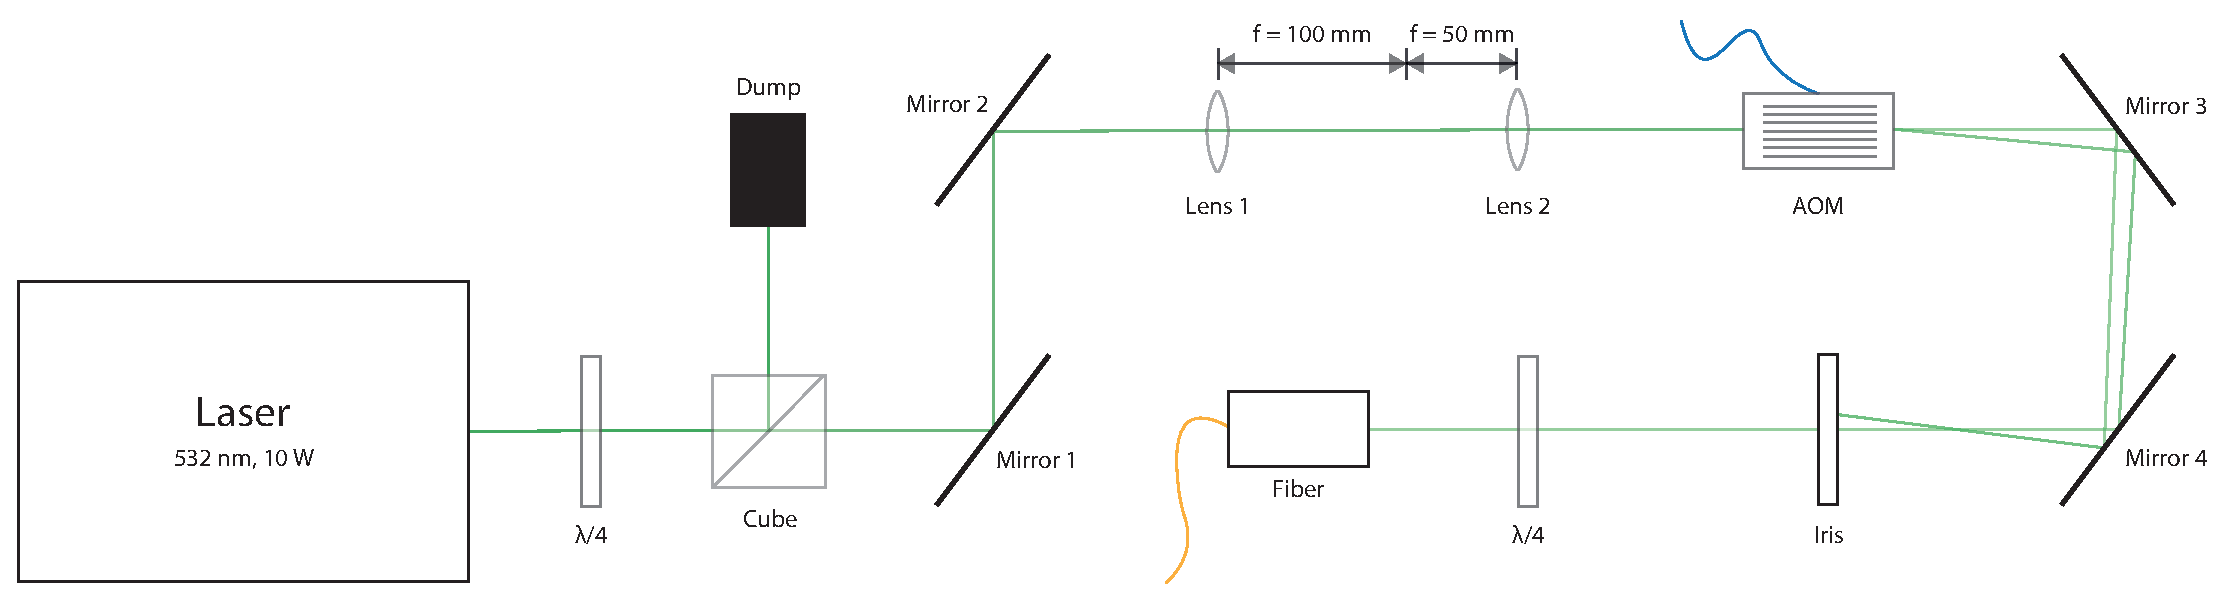
\includegraphics[width=\textwidth]{../figure/setup/power-reduction.pdf}
  \caption{Optical configuration of the power reduction section.
  }\label{fig:setup_power_reduction}
\end{figure}
The laser beam leaving the laser source is linearly polarized. In order to
divert the majority of the power into a beam dump we use a $\lambda/2$
retarder plate and a high-power polarizing beam splitter. Afterwards Mirror
\num{1} and Mirror \num{2} direct the beam towards the center of a $2:1$
telescope composed of Lens \num{1} and Lens \num{2}. The telescope is there to
reduce the beam diameter by \num{2} in order to avoid cut-off at the aperture
of the subsequent \gls{aom}. The \gls{aom} diffracts the laser beam into
multiple orders as it acts as a tunable diffraction grating. Mirror \num{3}
and Mirror \num{4} direct these orders onto a pinhole which is configured to
intromit only the first order deflection. The power in the first diffraction
order can be controlled by changing the \gls{rf} power sent to the \gls{aom}.
Finally a $\lambda/2$ retarder plate is used together with Mirror \num{3} and
Mirror \num{4} to couple the beam into the polarization-maintaining \gls{smf}.

\subsubsection{Beam deflection and detection}\label{subsec:setup_deflection_detection}

The section for beam deflection and detection as disclosed in
\Cref{fig:setup_beam_deflection} receives the down-powered laser beam from
the previously described section by a \gls{smf}. Hereinafter the beam passes
a rotatable retarder plate and beam splitter Cube \num{1} to clean the
polarization of the laser beam after passing through the \gls{smf}. A second
polarizer with Cube \num{2} is used to branch off a part of the beam to
Photodiode \num{1} that is positioned to be at the focal point of Lens
\num{1}. Photodiode \num{1} is connected via a feedback loop with the
amplitude modulation of the \gls{aom} depicted in
\Cref{fig:setup_power_reduction} to stabilize the laser intensity against, for
instance, thermal drifts.
\begin{figure}[htb]
  \centering
  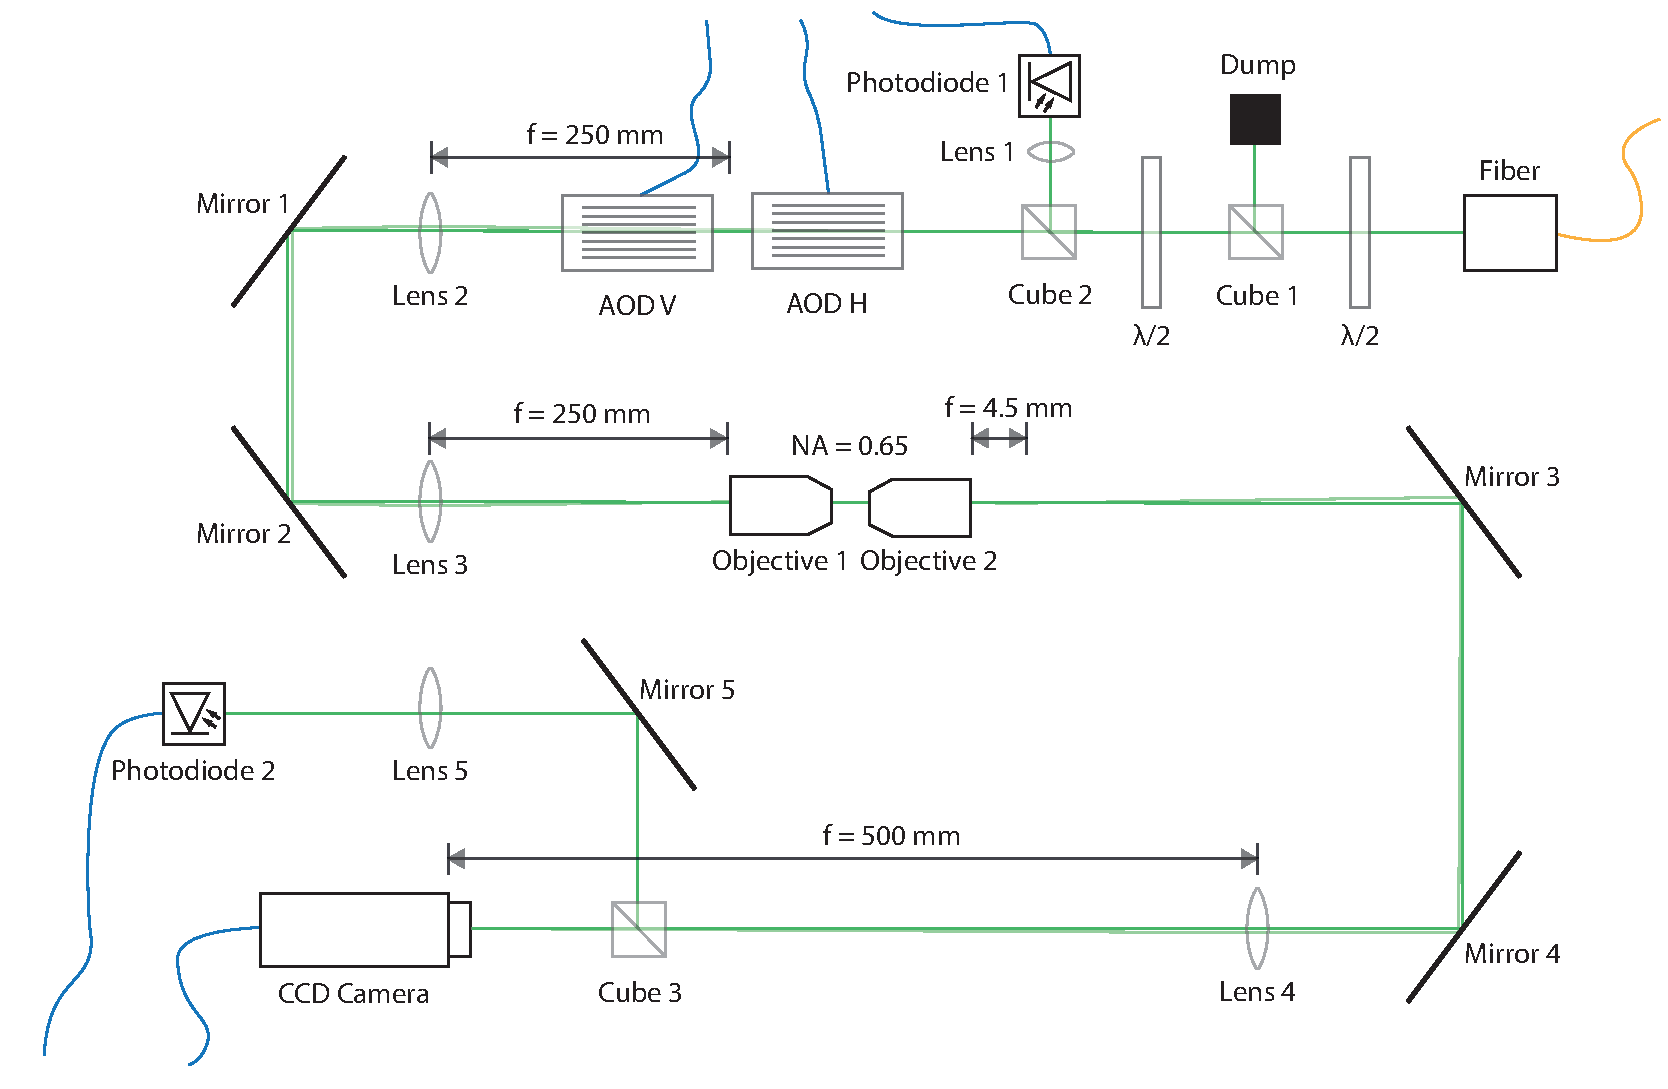
\includegraphics[width=\textwidth]{../figure/setup/beam-deflection.pdf}
  \caption{Optical configuration of the beam deflection section.
  }\label{fig:setup_beam_deflection}
\end{figure}
For horizontal and vertical beam deflection two \gls{aod}s are used. A $1:1$
telescope comprised of two lenses (Lens \num{2} and Lens \num{3}) is used to
image the beam on a pair of objectives. The purpose of the first objective is
to translate a change in the incident angle to a position offset in the atom
plane. The components described so far are sufficient to offset a
high-resolution pertubation laser perpendicular to the atomic plane. The
purpose of the other components is to unfocus the laser back for detection.
Combining the the focal length of the (second) objective $f_\text{obj}$ with
the focal length of $f_4$ we achieve a magnification of
\begin{equation}
  M
  =\frac{f_4}{f_\text{obj}}
  =\frac{\SI{500}{\milli\meter}}{\SI{4.5}{\milli\meter}}
  \approx 111
  \label{eq:setup_magnification}.
\end{equation}
The so colliminated and magnified laser beam is then imaged onto the \gls{ccd}
camera sensor. Cube \num{3} forks a portion of the beam away from the
\gls{ccd} camera on Mirror \num{5} that guides the beam towards Lens
\num{5} in order to focus the beam onto Photodiode \num{2}. It is important
that the sensor of Photodiode \num{2} is positioned on the focal spot of
Lens \num{5}, otherwise the laser beam would leave the sensor when deflected
by the \gls{aod}.

\section{Electronics}

Beforehand we described the optical setups used. Now we want to emphasize
on the electronics and how they are integrated into the optical setup.

In \Cref{fig:setup_elop_aom} the electronic setup of the \gls{aom} control
loop is presented. The \gls{dds} signal source outputs a \SI{80}{\mega\hertz}
\gls{rf} signal which is amplified and then supplied to the \gls{aom} for
intensity modulation, see \Cref{fig:setup_power_reduction}. Photodiode \num{1}
measures the modulated laser intensity and is connected to a \gls{pid}. The
\gls{pid} outputs a signal proportional to the deviation of the measured
intensity from the configured intensity which is provided to the amplitude
modulation input of the power amplifier.
\begin{figure}[htbp]
  \centering
  \begin{subfigure}[b]{0.4\textwidth}
    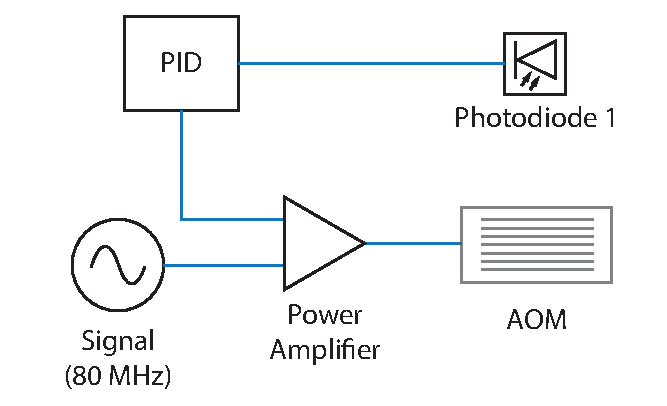
\includegraphics[width=\textwidth]{../figure/setup/aom-control.pdf}
    \caption{Intensity control via \gls{aom}.
    }\label{fig:setup_elop_aom}
  \end{subfigure}
  \begin{subfigure}[b]{0.4\textwidth}
    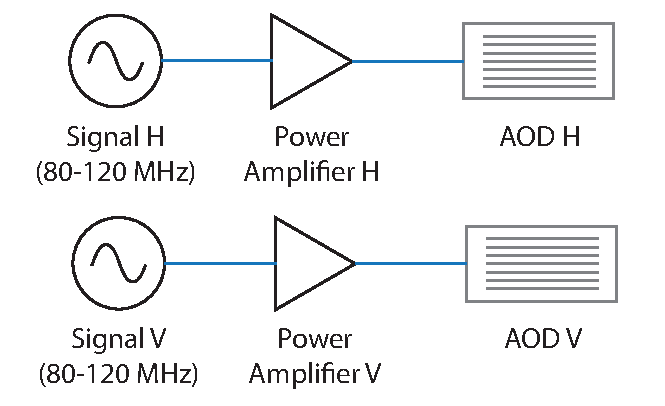
\includegraphics[width=\textwidth]{../figure/setup/aod-control.pdf}
    \caption{Deflection control via \gls{aod}.
    }\label{fig:setup_elop_aod}
  \end{subfigure}
  \caption{Electronic setup used to control the electro-optic devices.
  }\label{fig:setup_elop}
\end{figure}
In \Cref{fig:setup_elop_aod} the electronic setup connecting the \gls{2d}
\gls{aod} with the \gls{dds} signal sources are presented. The \gls{dds}
output is configured through a network interface as we will explain later.
Furthermore there is a reference signal source (not shown) that provides a
\SI{10}{\mega\hertz} reference signal to the \gls{dds}. First we will
elaborate on the general components used in \Cref{fig:setup_elop} as well as
our experiments.

\subsection{Signal source}\label{subsec:setup_signal_source}

We require the signal source to generate a sinusoidal \gls{rf} signal
\begin{equation}
  x(t)
  =A\cos\left(2\pi ft\right)
  \label{eq:signal},
\end{equation}
where $0\leq A\leq1$ denotes the amplitude and $f$ the frequency. For the
\gls{aom} setup in \Cref{fig:setup_elop_aom} it is sufficient to configure
a constant frequency $f=\SI{80}{\mega\hertz}$ and amplitude $A=1$, which is
further varied by the feedback loop. For the \gls{aod} control, however,
our requirements are beyond a constant signal. Ideally we would like to
program a time-dependent amplitude $A(t)$ and frequency $f(t)$, supplementary
to the support of an external trigger signal in order to syncronize multiple
signal sources. For our setup we chose to use \gls{dds} as signal sources as
they provide high frequency resolution, a wide range of modulation options and
are cheap compared to signal generators. In \cref{ch:digital_signal_synthesis}
we will give a more detailed view of the characteristics and limitations of
the \gls{ad9910}, the \gls{dds} \gls{ic} we use as signal source.

\subsection{Power amplifier}

We use three signal amplifiers with respective input from the signal sources
to have an output power of about $P=\SI{2}{\watt}$ required by the \gls{aod}s
and the \gls{aom} for maximum diffraction efficiency. The used amplifiers
offer a second input for external amplitude modulation. In case of the
\gls{aom} we connect this input to the output of the feedback loop.

\subsection{PID controller}

A feedback loop takes a reference $r(t)$, also called setpoint, and a process
variable $y(t)$ as input and outputs the value for a control variable $u(t)$,
which in turn, affects the process that determines $y(t)$. A \gls{pid} is
a specific implementation of such a feedback loop that uses a proportional,
differential and integrative term to estimate the control variable $u(t)$.
\begin{figure}[htb]
  \centering
  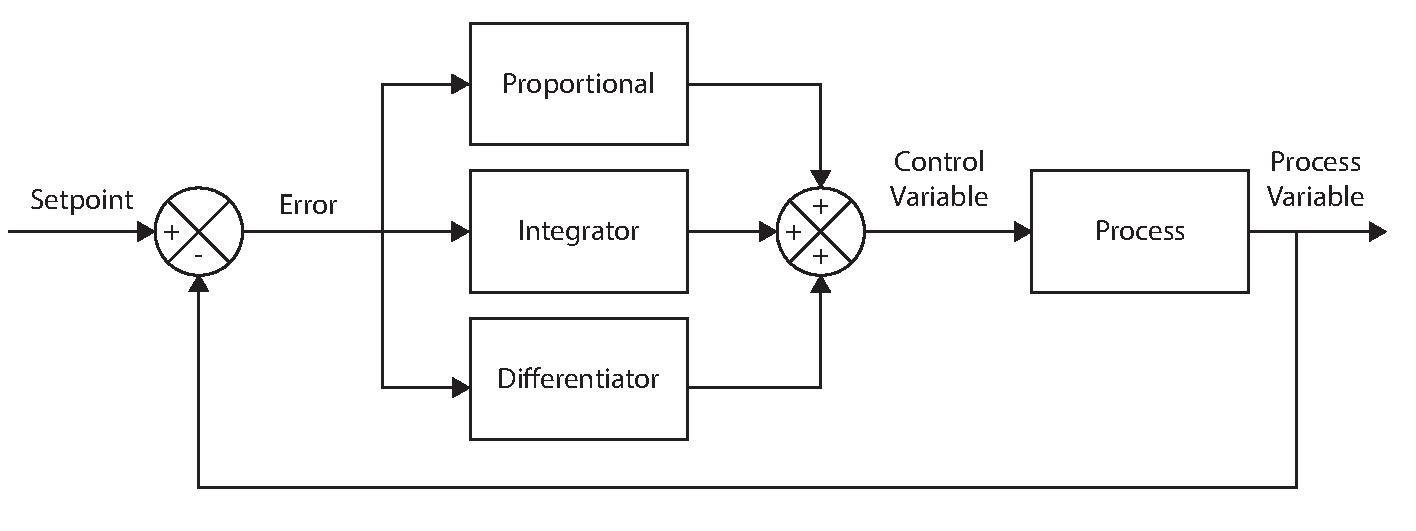
\includegraphics[width=\textwidth]{../figure/setup/pid-controller.pdf}
  \caption{Block diagram of a \gls{pid} feedback loop.
  }\label{fig:setup_pid}
\end{figure}
In \Cref{fig:setup_pid} we see a block diagram of a \gls{pid}. The error
values is supplied to the proportional block as well as the differentiator
and integrator which in sum give the updated control variable value $u(t)$.
The process changes with $u(t)$ and we read off the process variable $y(t)$
we want to regulate and feed it back to the start of the loop. The control
variable of the \gls{pid} can be expressed through
\begin{equation}
  u(t)
  =
  K_p e(t)+
  K_i \int_0^t \dd{t^\prime} e(t^\prime)+
  K_d \dv{t}{e(t)}
  \label{eq:setup_pid},
\end{equation}
where $K_p,K_i,K_d$ denote the coefficients of the respective terms. The ideal
values for the coefficients have to be found by loop tuning for each
application. Every term contributing to \cref{eq:setup_pid} can be thought
of to account for a different time scale of the process: the proportional term
considers the momentary error, the differential predicts trends and the
integrator corrects for past errors. For our particular application the
control variable is the amplitude $A(t)$ supplied to the modulation input
of the power amplifier of the \gls{aom} \gls{rf} signal. The process variable
of our \gls{pid} is the voltage measured at Photodiode \num{1}.

\subsection{Trigger source}

To syncronize the signal sources, the \gls{ccd} camera and the oscilloscope
it was necessary to design a network programable trigger source that outputs
a square pulse and forwards it to multiple devices. The schematics, board
layout and source code can be found in the \Cref{app:electronics:trigger_hub}.

\section{Communication}

In the last section of this chapter we will see that the diffraction
efficiency of the \gls{aod}s is not constant and requires readjustment by
amplitude modulation of the \gls{rf} signal supplied to the \gls{aod}s. We
consider this readjustment step as a calibration process. The efficienct
implementation of such a calibration process requires an orchestrated
interplay of different electronic devices which we will discuss now.
\begin{figure}[htb]
  \centering
  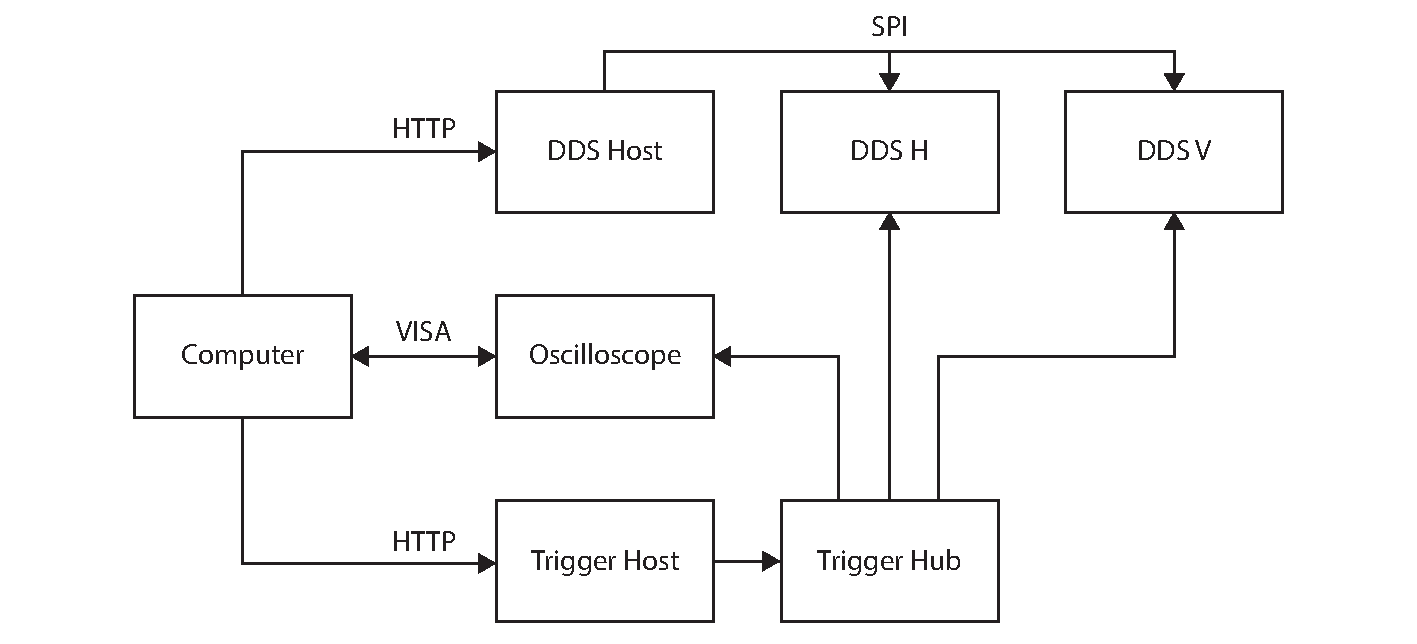
\includegraphics[width=\textwidth]{../figure/setup/network.pdf}
  \caption{Communication setup of the electronic devices in the experimental
    setup.
  }\label{fig:setup_network}
\end{figure}
In \Cref{fig:setup_network} the communication setup of our electronic devices
is illustrated. The computer, the trigger host, the oscilloscope and the
\gls{dds} host are connected to the \gls{lan}. The trigger host and the
\gls{dds} host are both \gls{bbb} that run a \gls{http} server from which the
computer can change parameters over the network. The implementation of the
\gls{http} server of the trigger host as well as the schematics of the trigger
hub can be found in \Cref{app:electronics:trigger_hub}. The \gls{http} service
that runs on the \gls{dds} host also contains a driver which writes the
\gls{dds} parameters over \gls{spi} to the respective \gls{dds} board. The
oscilloscope can be controlled through \gls{visa}.
\begin{listing}[htb]
  \inputminted[linenos,xleftmargin=.2\linewidth]{python}
  {../media/source/example.py}
  \caption{Example usage of the Python module to control the setup.
  }\label{lis:control_example}
\end{listing}
In \Cref{lis:control_example} we can see an examplary measurement using a
Python module we wrote to abstract away the interaction with the setup.

\section{Trial run}

After we integrated the \gls{dds} into the experimental setup, we wanted to
test its capabilities. Therefore we wrote a simple script that transforms
short letter sequences to a list of frequency pairs that we can playback
from the \gls{h} and \gls{v} \gls{dds}.
\begin{figure}[htb]
  \centering
  \begin{adjustbox}{width=\textwidth}
    \inputpgf{../figure/intensity/projection/}{bodo.pgf}
  \end{adjustbox}
  \caption{Text projection as captured by the \gls{ccd} camera.
  }\label{fig:setup_projection}
\end{figure}
In \Cref{fig:setup_projection} we see the projected text as captured by the
camera. The text projection is created by iterating through a set of frequency
pairs, which as we know, correspond to a position offset. For a sufficient
exposure of the \gls{ccd} camera we can capture a time average over all
single points just as we plan to do with the optical potentials. Even though
we configured the \gls{dds} with constant amplitude, we notice that the
illumination is not homogenous. In fact we will see that the diffraction
efficiency of the \gls{aod} depends heavy on the frequency and it will
turn out to be a challenging endeavour trying to compensate for this
dependency as we will see in the final part of this thesis.

\chapter{Signal measurements}

By the time the \gls{rf} signal has reached the piezoelectric of the
\gls{aod} it has been synthesized from a reference signal, amplified to match
the power requirements of the \gls{aod} and matched to the impedance of the
\gls{aod}. Each of these stages ammends the shape of the \gls{rf} signal and
as we will see introduce new frequency responses of the amplitude. The so
inevitable amplitude modulation affects the deflected intensity of the laser
beam and will lead to the intensity characteristics discussed in the next
chapter.

\section{Digital signal synthesis}

As has been described in the experimental setup section, \gls{dds} are used
for signal synthesis. In the present section we want to examine the
frequency behaviour of the \gls{dds}. In particular we are interested how the
amplitude responds to different frequencies and how the digital design of the
\gls{dds} affects the \gls{rf} signal shape.

\subsection{Setup}
\label{subsec:signal_synthesis_setup}

For the following experiments we configured the \gls{dds} to do a linear
frequency sweep from \SI{80}{\mega\hertz} to \SI{120}{\mega\hertz} at a sweep
duration of \SI{26.84}{\micro\second}. The frequency range has been choosen
because it overlaps with the operation range required to drive the \gls{aod}.
The sweep duration is a good compromise between being able to resolve the
complete sweep with limited oscilloscope resolution on the one hand and
limited frequency resolution of the synthesizer.

The time resolution of most oscilloscopes depends on the selected time scale,
however choosing a finer time scale entails shortening the time length, thus
we have a trade-off between being able to perform signal analysis that demands
fine resolution of the sinusoidal voltage and the number of measurements we
need to perform to capture a complete passthrough of the synthesized signal
cycle. We found that a selected time division of \SI{10}{\micro\second} is
sufficient for signal analysis, i.e. \gls{fft}, but at the same time limits
the number of measurements to the magnitude of hundreds.

To overcome the obstacle that we can only capture one time window of a
\gls{rf} signal passthrough we inserted a frequency generator between the
external trigger source and the oscilloscope. The frequency generator is
configured to emit a square wave pattern on the rising edge of the external
trigger of width $d$. The oscilloscope was configured to be triggered on the
falling edge of the external trigger signal supplied by the frequency
generator. By adjusting the square wave width $d$ we effectively added a
delay to the trigger signal. In order to capture now the complete signal over
duration $T$ we incremented the delay $d$ in steps of $T/300$.

\subsection{Results}
\label{subsec:signal_synthesis_results}

The former setup produced a single dataset we evaluated from two different
angles. First we explored how the digital design of the \gls{dds} propagates
into the signal. Second we explored the frequency dependence of the amplitude.

\subsubsection{Spectrogram}

A spectrogram visualizes how the frequency spectrum varies in time. One way
to obtain a spectrogram is to partition the data into overlapping time chunks
while performing \gls{fft} which allows us to combine time and frequency
domain specific characteristics. In our case we choose the relative spectral
power to be encoded through color.

\begin{figure}[h]
  \centering
  \includegraphics[width=\textwidth]{\figuredir{signal/synthesis/spectrogram.pdf}}
  \captionsetup{width=.8\textwidth}
  \caption{Spectrogram of delayed time windows of the \gls{dds} output signal
    configured to perform a frequency sweep from \SI{80}{\mega\hertz} to
    \SI{120}{\mega\hertz}. For an ideal linear sweep we would expect a linear
    timeline of the frequency, instead we observe a discrete set of
    frequencies which reflects the digital nature of the \gls{dds}.}
  \label{fig:signal_synthesis_spectrogram}
\end{figure}

\Cref{fig:signal_synthesis_spectrogram} depicts four spectrogram, each taken
at a different time window of the frequency sweep passthrough. The first
spectrogram captures the start of the frequency sweep. We can see how for the
first \SI{200}{\micro\second} the \gls{dds} outputs only the start frequency
of \SI{80}{\mega\hertz} which then is increased by increments to reach the
final frequency of \SI{120}{\mega\hertz} as can be seen in the lower right
spectrogram at the end of the frequency sweep.

For an ideal frequency sweep we would expect a linear timeline of the
frequency, instead we see that \gls{dds} outputs a discrete set of
frequencies.

\subsubsection{Amplitude frequency response}

Although the previous section satisfied our curiousity it did not disclose
anything we did not expect. Anyhow, in this part we examine the amplitude
frequency response which by all means has great significance on the observed
intensity patterns we discuss later.

\begin{figure}[h]
  \centering
  \includegraphics[width=\textwidth]{\figuredir{signal/synthesis/frequency-max-amplitude.pdf}}
  \captionsetup{width=.8\textwidth}
  \caption{Maximum amplitude of the two \gls{dds} at different frequencies
  during linear sweep operation. In the two lower curves the \gls{dds} were
configured with enabled inverse sinc filter that is supposed to compensate
frequency dependence in the amplitude.}
  \label{fig:signal_synthesis_frequency_max_amplitude}
\end{figure}

To find the frequency dependency of the amplitude we carried out \gls{fft} on
the voltage of the respective time window and extracted the dominant
frequency located at the maximum of the power spectrum and thereby reduced
each measurement to a frequency and corresponding maximum amplitude.

The result is visualized for the two different signal sources with different
filter mode in \Cref{fig:signal_synthesis_frequency_max_amplitude}. We observe
that there is no significant difference between distinct \gls{dds}. The
inverse sinc filter proclaimed to reduce frequency dependence of the amplitude
only reduced the output amplitude without changing the overall frequency
response characteristics.

\subsection{Summary}

At the signal source stage the \gls{dds} already induce significant frequency
dependency of the output amplitude. The built-in inverse sinc of the \gls{dds}
does not reduce this dependency, therefore we disable the inverse sinc
filter for all other measurements. Eventually we could confirm the
discreteness of the frequency domain produced by the \gls{dds}.

\section{Signal amplification}

The \gls{rf} signal supplied by the synthesizer is too weak to power the
\gls{aod}, therefore we supply the synthesized signal to an amplifier and
feed the amplified signal to the \gls{aod}. The amplification acts as the
second stage in our \gls{rf} signal processing and we expect it to amend
the frequency behaviour of the amplitude.

\subsection{Setup}

The measurement algorithm described in \cref{subsec:signal_synthesis_setup} is
still valid for the now amplified signal. Even though we found in the former
section that the synthesized signal does not differ in between different
\gls{dds} we supplied the horizontal \gls{dds} to the respective amplifer.

The amplified signal should be of approximate power \SI{33}{\decibel\meter}.
At the usual \SI{50}{\ohm} in between coaxial cables this corresponds to an
approximate voltage of \SI{10}{\volt}. Even though the employed oscilloscope
is rated for more then \SI{10}{\volt} when being used in \SI{1}{\mega\ohm}
mode we inserted a chain of attentuators (from coaxial cable to
oscilloscope: \SI{1}{\decibel}, \SI{3}{\decibel}, \SI{6}{\decibel},
\SI{10}{\decibel} and \SI{10}{\decibel} to distribute heat dissipation) in
between the coaxial cable and the oscilloscope input to attain a total
damping of \SI{30}{\decibel}.

\subsection{Results}

The analysis is analogue to the frequency response part in
\cref{subsec:signal_synthesis_results} in that we perform \gls{fft} on each
measurement window to extract the dominant frequency with the maximum
amplitude in the time domain. The maximum amplitude is very close to the
effective amplitude of a sinusoidal signal, yet it is much easier to extract
from the time series data.

In a second step we normalized the so obtained amplitude frequency response
of the amplified signal with the previously evaluated source signal amplitude
frequency response. The specific normalization used was a min-max type where
we subtracted the minimum amplitude from each signal and divided the
difference by the new value range.

The spectrogram of the amplified signal should be equal to
\Cref{fig:signal_synthesis_spectrogram}, hence not give us any new insights.

\subsubsection{Amplitude frequency response}

\Cref{fig:signal_amplification_frequency_max_amplitude} presents us the
damped output signal subject to the signal frequency after amplification for
the two distinct amplifiers. We require two distinct amplifiers because our
setup comprises two independently controlled \gls{aod}.

\begin{figure}[ht]
  \centering
  \includegraphics[width=\textwidth]{\figuredir{signal/amplification/frequency-max-amplitude.pdf}}
  \captionsetup{width=.8\textwidth}
  \caption{Maximum amplitude at dominant frequency per delayed window for two
  different amplifiers. We can see the discreteness of the frequency domain
from the digital signal synthesis as well as three resonances. Further the
amplifier differ by a constant offset.}
  \label{fig:signal_amplification_frequency_max_amplitude}
\end{figure}

At first we note that the amplified signal differs by a constant offset. We
assume this offset to be caused by different component quality as the
frequency response shape itself is similar. On a
second glance we again find evidence for discrete frequencies from
\Cref{fig:signal_amplification_frequency_max_amplitude} when we emphasize the
subtile horizontal pattern of the markers.

\subsubsection{Comparison with source signal}

\Cref{fig:signal_amplification_comparison} shows the min-max-normalized
amplified signals with the min-max-normalized input signal from the horizontal
\gls{dds}. After normalization the fixed offset difference, we observed
previously in between the distinct amplifiers, vanishes and the same
frequency response shape is obvious.

\begin{figure}[ht]
  \centering
  \includegraphics[width=\textwidth]{\figuredir{signal/amplification/comparison.pdf}}
  \captionsetup{width=.8\textwidth}
  \caption{Relative amplitude at dominant frequency per delayed window for
  two different amplifiers and their digital signal source. In comparison to
the signal source the amplifiers introduce a further resonance at the
center frequency.}
  \label{fig:signal_amplification_comparison}
\end{figure}

Comparison of the signal after (black, green) and before amplification (red)
yields that the input signal from \gls{dds} seems more dense than after the
amplification, yet we miss a solid explaination for this behaviour as the
amplification process uses analogue components. It could be that the voltage
resolution of the oscilloscope was misconfigured to a to coarse scaling.
Furthermore we observe that the amplifier remedies the amplitude drop
at around \SI{102}{\mega\hertz} of the source signal. However the amplifier
possess resonacnes around \SI{98}{\mega\hertz} and \SI{110}{\mega\hertz}
where the amplitudes drop.

\subsection{Summary}

To sum up we found that distinct amplifier differ by a fixed voltage offset.
Furthermore the amplifiers introduce new resonances into the amplitude
frequency response and posseses a more discrete signal spectrum then the
input signal.

\section{Signal reflection}

In the previous sections we explored the signal transfer at the synthesis
and amplification stage. The last stage that is accessable to us without
destruction of the \gls{aod} concernse the power reflection at the \gls{aod}
itself. From the reflection we can deduce the power transmission, hence for
a large reflection we would expect a small transmission and in that sense
less beam intensity in the first deflection order.

\subsection{Setup}

The power reflection measurements were conducted with a network analyzer. In
a first embodiment of the experiment we directly supplied the \gls{aod}
through a coaxial cable of the network analyzer with power and measured the
reflection. In a second embodiment we used a direct-coupler to supply the
respective amplifier with a signal and measure the reflection through the
direct-coupler to avoid harm to the network analyzer because the network
analyzer is not able to provide \SI{2}{\watt} of output power as required
by the \gls{aod}.

\subsection{Results}

At first we discuss the reflection spectrum of the direct connection of
the network analyzer and the distinct \gls{aod} elements. Thereafter we
analyze the reflection spectrum of the direct-coupler and then continue with
the reflection spectrum with an amplified signal. Finally we compare the
direct and amplified spectra.

\subsubsection{Direct connection}

\Cref{fig:signal_reflection_direct} visualized the power reflection spectrum
of both \gls{aod} elements when direct coupled to the network analyzer at
the maximum output power of \SI{10}{\decibel\meter}.

\begin{figure}[ht]
  \centering
  \includegraphics[width=\textwidth]{\figuredir{signal/reflection/direct.pdf}}
  \captionsetup{width=.8\textwidth}
  \caption{We see the signal reflection of the two different \gls{aod} when
  connected directly to the network analyzer. We can see that both crystal
differ in their respective spectrum.}
  \label{fig:signal_reflection_direct}
\end{figure}

Most interesting finding in \Cref{fig:signal_reflection_direct} is that the
power reflection shows very different behaviour in between the distinct
\gls{aod} elements. The \gls{aod} anticipated for the vertical deflection
is most transmissive at \SI{97}{\mega\hertz} with transmission falling of
on both sides while the \gls{aod} anticipated for the horizontal deflection
has two local transmission maxima and a rather bad transmision near the center
frequency.

\subsubsection{Direct-coupler}

The direct-coupler is an apparatus comprising a coaxial input and output
port as well as a coaxial input reflection and output reflection port. It is
disignated to measure the reflection of a (possible) high power signal
without jeopardizing measurement equipement.

\begin{figure}[ht]
  \centering
  \includegraphics[width=\textwidth]{\figuredir{signal/reflection/coupler.pdf}}
  \captionsetup{width=.8\textwidth}
  \caption{Input power reflection when supplying the direct-coupler with
    \SI{-10}{\decibel\meter} input signal and reflection at the output of
    the direct-coupler while other ports are closed with \SI{50}{\ohm}}.
  \label{fig:signal_reflection_coupler}
\end{figure}

In \cref{fig:signal_reflection_coupler} we see the reflection spectrum for
the case that we provide the network analyzer output signal to the input of
the direct-coupler and connect the reflection output of the direct-coupler
with the second network analyzer port while the remaining ports are under
\SI{50}{\ohm} closure.

We note that the reflection measured at through the direct-coupler is lowered
by many orders of magnitude compared to the input signal but essentially of
the same shape. The noise in the reflection is very high because of the low
power supplied into the direct-coupler.

\subsubsection{Amplification coupled}

We now use the direct-coupler to measure the output reflection at the
\gls{aod} elements after the signal was amplified.

\begin{figure}[ht]
  \centering
  \includegraphics[width=\textwidth]{\figuredir{signal/reflection/coupled.pdf}}
  \captionsetup{width=.8\textwidth}
  \caption{Reflection at the direct-coupler output after amplification of the
  network analyzer input signal for different effective powers. We see that
the applied power does not effect the spectrum.}
  \label{fig:signal_reflection_coupled}
\end{figure}

In \Cref{fig:signal_reflection_coupled} we see the effective reflection
spectrum for the distinct \gls{aod} elements. The effective reflection
spectrum is obtained when subtracting the input reflection from the output
reflection.

\subsubsection{Comparison}

In the previous part we saw that the reflection spectrum does not show any
power dependence, thus we should be able to compare the spectrum we obtained
directly with the amplified result.

\begin{figure}[ht]
  \centering
  \includegraphics[width=\textwidth]{\figuredir{signal/reflection/comparison.pdf}}
  \captionsetup{width=.8\textwidth}
  \caption{Comparison of reflection from amplified input signal and direct
  signal provided from the network analyzer. The different reflection spectrum
can be associated to the amplifier.}
  \label{fig:signal_reflection_comparison}
\end{figure}

In \Cref{fig:signal_reflection_comparison} we can see how there is additional
reflection from the amplifier, nevertheless the global spectrum
characteristics stay in place.

\subsection{Summary}

Distinct \gls{aod} elements show different power transmission characteristics
and the amplifier only causes marginal shifts. Examination of the \gls{aod}
elements in details discloses different impedance matching circuits.

Impedance matching is used to reduce power reflection by providing a constant
input resistance of \SI{50}{\ohm} accross an ideally wide frequency range.
Still the impedance differs between the \gls{aod}s. We assume that the
crystal properties i.e. cut, purity are responsible for that.

By the previous reflections measurements we keep in mind that these were
conducted with an input signal with fairly homogenous amplitude. From the
previous sections we know that this in fact is not the case for the \gls{rf}
signal later used.

\chapter{Intensity measurements}

In the previous chapter we seeked for different aspects of the \gls{rf}
signal powering the \gls{aod} elements. Down the road we had to realize that
there are many forces at work which at large are difficult to account for.

That in mind we proceed with the analysis of the deflected laser beam
intensity subject to the configured frequency and relative amplitude of the
synthesized output \gls{rf} output signal.

\section{Intensity control}

The laser intensity is regulated by a control loop with \gls{aom} in order to
intercept power drifts from the laser source. This control loop is tightly
integrated into our experimental setup and thus will be present for all
subsequent intensity measurements. In this section we want to discuss the
grade of this control loop and estimate the error contribution.

\subsection{Setup}

The experimental setup is the same as described in XX but with disassembled
\gls{aod}. The photodiode gain was set to \SI{50}{\decibel} so that we can
easily compare measurements.

\subsection{Long term measurement}

In the long term measurement we were interested in the long term behaviour
of the intensity control loop. In particular if there are oscillations or
intensity collapses.

Therefore we obtained voltage measurements in an interval of about
\SI{2}{\minute} over a total time of approximately \SI{16}{\hour}.

\begin{figure}[ht]
  \centering
  \includegraphics[width=\textwidth]{\figuredir{intensity/control/long.pdf}}
  \captionsetup{width=.8\textwidth}
  \caption{Long term measurement of the intensity with controlled intensity.
    The intensity was measured every \SI{2}{\minute} for over \SI{16}{\hour}
    to determine the accuracy of the intensity controller. The outlier at
    about 22:45 was caused by laboratory visit otherwise the intensity remains
  stable.}
  \label{fig:intensity_control_long}
\end{figure}

The voltage time series is shown in \Cref{fig:intensity_control_long}. We 
note outliers at about 22:45 which were probably caused by a late laboratory
visit. Further we see a constant albeit noisy intensity signal. In comparison
we could watch real time oscillations and drifts when disabling the control
loop.

\Cref{tab:intensity_control_long} depicts the descriptive statistics belonging
to the voltage time series visualized in \Cref{fig:intensity_control_long}.
The mean intensity is measured to be around \SI{6.79}{\volt} with peaks up
to \SI{6.86}{\volt}. The standard deviation yields us a relative error of
around \SI{1.4}{\percent}.

\begin{table}[h]
  \centering
  \begin{tabular}{|c|c|c|c|}
    \hline
    Mean & Minimum & Maximum & Standard deviation \\
    \hline
    \SI{6.79}{\volt} &
    \SI{4.88}{\volt} &
    \SI{6.86}{\volt} &
    \SI{0.09}{\volt} \\
    \hline
  \end{tabular}
  \captionsetup{width=.8\textwidth}
  \caption{Descriptive statistics of the short term measurement of the
  intensity with controlled intensity. Note the small standard deviation.}
  \label{tab:intensity_control_long}
\end{table}

\subsection{Short term measurement}

The previous section gave us already some good insights about the long term
stability of the intensity control loop. Yet in practice typical intensity
measurements are of much smaller magnitude, henceforth it seems close at hand
to also conduct a short term measurement.

\begin{table}[h]
  \centering
  \begin{tabular}{|c|c|c|c|}
    \hline
    Mean & Minimum & Maximum & Standard deviation \\
    \hline
    \SI{6.78}{\volt} &
    \SI{6.77}{\volt} &
    \SI{6.82}{\volt} &
    \SI{0.01}{\volt} \\
    \hline
  \end{tabular}
  \captionsetup{width=.7\textwidth}
  \caption{Descriptive statistics of the short term measurement of the
  intensity with controlled intensity. Note the small standard deviation.}
  \label{tab:intensity_control_short}
\end{table}

For the short term measurement time parameters were adjusted to a sample
interval of \SI{10}{\second} and measurment were performed over \SI{1}{\hour}.

\begin{figure}[ht]
  \centering
  \includegraphics[width=\textwidth]{\figuredir{intensity/control/short.pdf}}
  \captionsetup{width=.8\textwidth}
  \caption{Short term measurement of the intensity with controlled intensity.
    The intensity was measured every \SI{10}{\second} for over \SI{1}{\hour}
    to determine the accuracy of the intensity controller.}
  \label{fig:intensity_control_short}
\end{figure}

The intensity time series of the short term measurement is depicted in
\Cref{fig:intensity_control_short} and the associated descriptive
statistics are presented in \Cref{tab:intensity_control_short}.

On a smaller timescale we see that the intensity control loop performs
periodic oscillations, however the descriptive statistics show much smaller
deviation from the mean, than observed in the long term measurements. As we
do not see outliers in \Cref{fig:intensity_control_short} we can pay more
attention to the value range of \SI{0.05}{\volt} which was obfuscated in
the long term measurement because of outliers.

\subsection{Summary}

The previous discussion confirmed that the intensity is regulated in that
we only observe oscillations around the targeted intensity value. Yet we are
still missing statements with regard to the magnitude of these oscillations
as we are missing a comparison to real intensity data.

\begin{table}[ht]
  \centering
  \begin{tabular}{|c|c|c|}
    \hline
    Measurement & Value range & Standard deviation \\
    \hline
    long term & \SI{1.98}{\volt} & \SI{0.09}{\volt} \\
    \hline
    short term & \SI{0.06}{\volt} & \SI{0.01}{\volt} \\
    \hline
    typical & \SI{1.43}{\volt} & \SI{0.40}{\volt} \\
    \hline
  \end{tabular}
  \captionsetup{width=.8\textwidth}
  \caption{Descriptive statistics of the short and long term measurement
  of the intensity control and a typical intensity measurements where we
subtracted the mean intensity for comparison.}
  \label{tab:intensity_control}
\end{table}

For a typical measurement, to compare the intensity oscillations with, we
elected the intensity progression of a linear frequency sweep of the
\gls{aod} in the vertical socket while the \gls{aod} in the horizontal socket
is fixed. We will discuss this specific meausurement in detail in a later
section. In \Cref{tab:intensity_control} we see some statistics of the
long and short term measurements next to the typical measurement.

\begin{figure}[ht]
  \centering
  \includegraphics[width=\textwidth]{\figuredir{intensity/control/deviation.pdf}}
  \captionsetup{width=.8\textwidth}
  \caption{Boxplot of the long and short term intensity measurements and a typical
  intensity measurement with the \gls{aod} where we subtracted the mean intensity
  for comparison. The typical measurements covers a much wider intensity range
then deviations from the intensity control loop.}
  \label{fig:intensity_control_comparison}
\end{figure}

One dismally error estimate would be the quotient of the value range of the
short term measurement and the typical measurement, yielding an error of
\SI{4.2}{\percent}. A second approach would be the quotient of the standard
deviation of the short term and typical measurement, yielding
\SI{2.5}{\percent} error. When comparing the typical measurement to the
statictis of a long term measurement we find rather large errors which
suggests that there re other statistical key figures which may be more
suitable.

A boxplot is very useful in visualizing the spread. We have an orange stripe
marking the median, the contour of the box marking the data between first and
third quantil. The usual value range is marked by the whiskers and outliers
are marked as the circles outside the whiskers.
In \Cref{fig:intensity_control_comparison} we see such a boxplot for the
absolute deviation from the mean of the three measurements. The absolute
deviation from the mean accounts for the different transmission just because
of the presence of the \gls{aod} in the typical measurement but keeps the
linear scale unlike the squared deviation from mean. We can see that in a
typical measurement (upper boxplot) the usual deviation from mean is much
larger than for the short and long term measurement of the intensity
regulation.


\section{Gaussian beam profile}

With the previously described calibration steps in place we can assess the
final quality of the beam with an image capture of the \gls{ccd} camera in the
aligned setup \cref{sec:deflection}.

\begin{figure}[ht]
  \centering
  \includegraphics[width=.5\textwidth]{\figuredir{intensity/profile/profile2d.pdf}}
  \caption{Image detail from the captured beam with the \gls{ccd} camera.}
  \label{fig:beamprofile:2d}
\end{figure}

The two dimensional beam profile shows the characteristical two dimensional
gaussian distribution with diffraction rings caused by beam clipping at
finite apertures as described in \cite{Hertlein2017}.

\begin{figure}[ht]
  \centering
  \includegraphics[width=\textwidth]{\figuredir{intensity/profile/profile1d.pdf}}
  \caption{1D horizontal and vertical profile extracted from the center of
    the image detail in \cref{fig:beamprofile:2d} with fitted gaussian curve
  and residue.}
  \label{fig:beamprofile:1d}
\end{figure}

By inspecting the one dimensional profiles with fitted gaussian and residue
we again confirm conclusions drawn in \cite{Hertlein2017}. The clipped top
of the measured intensity originates from the saturated pixels of the
\gls{ccd} camera and can be ignored. We further observe a slight assymmetry
at the diffraction rings. Overall the shown profiles can be considered to
confirm a good alignment.

\chapter{Intensity optimization}

% at different amplitude values
% without amplitude modulation
% with amplitude modulation

\chapter{Conclusion}

\section{Summary}

\section{Future Outlook}

\section{Further Applications}


\printglossaries
\listoffigures
\listoftables
\listoflistings
\printbibliography

\appendix
\chapter{Electronics}

\section{Direct Digital Synthesizer}
\label{app:elec:dds}

\subsection{Operating Range}

In the subsequent calculations we refer to our specific use case as laid out
in \cref{sec:elec:dds}.

We apply a reference signal of
\begin{equation}
  f_\text{ref}=\SI{10}{\mega\hertz}
\end{equation}
configured to be used with a \gls{pll} multiplier of
$N=100$ yielding a system clock of
\begin{equation}
  f_\text{sys}=Nf_\text{ref}=\SI{1}{\giga\hertz}.
\end{equation}
The timer clock used for the linear ramp and memory playback runs with
a quarter of the system clock
\begin{equation}
  f_\text{timer}=f_\text{sys}/4=\SI{250}{\mega\hertz}.
\end{equation}

The \gls{ad9910} uses a \SI{14}{\bit} \gls{asf} and \SI{32}{\bit} \gls{ftw}
to parameterize amplitude $A(t)$ and output frequency $f(t)$ by
\begin{align}
  FTW
  :=
  \left\lfloor2^{32}\left(\frac{f_\text{out}}{f_\text{sys}}\right)\right\rceil
  &&
  ASF
  :=
  \left\lfloor\frac{A_\text{out}}{2^{14}}\right\rceil
  \label{eq:elec:ftwasf}
\end{align}
wherein $\lfloor{\cdot}\rceil$ rounds the given float to the nearest integer.
The theoretical limit for the maximum output frequency then is found via
\begin{equation*}
  f_\text{max}
  =
  \left(1-\frac{2^{31}-1}{2^{32}}\right)f_\text{sys}
  =
  \left(\frac{1}{2}-\frac{1}{2^{31}}\right)f_\text{sys}
  \approx
  \frac{1}{2}f_\text{sys}
  =
  \SI{500}{\mega\hertz}.
\end{equation*}
Yet the datasheet \cite{AD9910} reports $f_\text{max}=\SI{420}{\mega\hertz}$
and in fact we found the output signal to be very noisy at the theoretical
limit.

We continue with the assessment of the digital ramp that does a unidrectional
linear sweep on the frequency from \SI{90}{\mega\hertz} to
\SI{110}{\mega\hertz}. The digital ramp of the \gls{ad9910} lets us define
a \gls{ftw} step $M$ word of \SI{32}{\bit} as well as a step rate word $S$ of
\SI{16}{\bit} resolution. They relate to the frequency step and the time
step through
\begin{align}
  \Delta f
  =
  \frac{M}{2^{32}}f_\text{sys}
  &&
  \Delta t
  =
  \frac{S}{f_\text{timer}}
  =
  \frac{S}{4f_\text{sys}}.
  \label{eq:elec:step}
\end{align}
The sweep duration is deterimened by $S,M$ through
\begin{equation}
  T_\text{duration}
  =
  \frac{f_\text{upper}-f_\text{lower}}{\Delta f}\Delta t
  =
  2^{32}\frac{f_\text{upper}-f_\text{lower}}{f_\text{sys}}\frac{S/M}{f_\text{timer}}
\end{equation}
for a target sweep duration of $T_\text{duration}=\SI{10}{ms}$ we find
\begin{equation*}
  \frac{S}{M}
  =
  \frac{T f_\text{timer}}{2^{32}}\frac{f_\text{sys}}{f_\text{upper}-f_\text{lower}}
  =
  \frac{10^9}{2^{35}}
  \approx
  \num{2.9104e-2}
  =
  \frac{1819}{62500}
\end{equation*}
the last step can be obtained by best ratio approximation using continued
fractions as for example described in \cite{Ashley2003}. It should be kept in
mind that the best ratio approximation is likable to introduce an error,
therefore realistic durations may differ from the configured value and it
is possible that better approximations exist that allow smaller $\Delta f,
\Delta t$, thus providing a sweep resolution. In the above case the given
time duration translates to
\begin{align*}
  \Delta f
  =
  \frac{62500}{2^{32}}f_\text{sys}
  \approx
  \SI{145}{\kilo\hertz}
  &&
  \Delta t
  =
  \frac{1819}{f_\text{timer}}
  \approx
  \SI{7.28}{\micro\second}
\end{align*}
or $(f_\text{upper}-f_\text{lower})/\Delta f=138$ discrete data points.

Eventually we are left with the assessment of the amplitude sequence. The
memory fits at most 1024 discrete amplitude values and the \gls{ad9910}
allows us to set the time spent at each amplitude value via the \SI{16}{\bit}
playback rate $P$ word
\begin{equation}
  \Delta t
  =
  \frac{P}{f_\text{timer}}
  =
  \frac{4P}{f_\text{sys}}
\end{equation}
which gives us range from $\min\Delta t=\SI{4}{\nano\second}$ to
$\max\Delta t=\SI{26.14}{\micro\second}$. As we incorporate all of the 1024
data points this gives us a duration range from about
$\min T=\SI{4}{\micro\second}$ to $\max T=\SI{26.84}{\milli\second}$.

\section{Trigger Source}
\label{app:elec:trig}

\begin{figure}[h]
  \centering
  \includegraphics[width=\textwidth]{images/circuit/line-driver/scheme.pdf}
  \caption{Schematic of trigger source amplifier with digital input
  and four \gls{sma} connectors.}
  \label{fig:elec:trig:scheme}
\end{figure}

\begin{figure}[h]
  \centering
  \includegraphics[width=.4\textwidth]{images/circuit/line-driver/board.pdf}
  \caption{Board layout of trigger source amplifier fitted to be mounted on
  top of the BeagleBone Black headers.}
  \label{fig:elec:trig:board}
\end{figure}

\chapter{Calibration}

\textit{Alterations of the laboratory environment combined with the exchange
of components from the original setup made it necessary to recalibrate the
setup. In this chapter we want to document the calibration steps required to
reproduce the claimed results.}

\section{Fiber coupling}

The visually shielded section of the setup, used to reduce the output power
of the laser source, is optically paired with the open section for beam
deflection via a \gls{smf} that only permits two orthogonal polarization and
a single gaussian mode. By tuning the polarisator inside the power
reduction section we can try to match one of the orthogonal polarization
modes supported by the \gls{smf}. Polarization discrepancies cause the
polarization inside the \gls{smf} to oscillate with vibrations or changes in
temperature, henceforth it is key to couple polarization modes in order to
ensure a stable operation. A strategy proven to find an approximate
polarization match between the laser beam and the \gls{smf} is presented. In
addition to the setup described in \cref{subsec:setup_power_reduction} and
\cref{subsec:setup_deflection_detection} an oscilloscope and a hot air gun
were used.
\begin{enumerate}
  \item Connect the photodiode to the oscilloscope and use a coarse time
    scale (i.e. \SI{2}{\second}).
  \item Apply appropriate laser safety glasses and inform present personal
    of the imminent danger.
  \item Open the cover of the power reduction setup.
  \item Apply heat to the \gls{smf} through the hot air gun, alternatively
    you can try to move the fiber.
  \item The photodiode signal should start to oscillate. Tune the polarizor
    inside the power reduction subject to minimizing the oscillation.
\end{enumerate}
The oscillations occur as the polarization circulates inside the fiber and
will stop at some point when a new equilbrium has been established. In this
case remove the heat or mechanical stress on the fiber and wait before you
reapplying new impetus.

\section{Beam alignment}

Beams that pass off-centered through spherical lenses experience optical
aberrations, additionally uncentered beams may cause further optical defects
from reflections or clipping at boundaries. Since most changes to the optical
setup outdate the previous beam alignment, hence making the realignment
a rather frequent procedure, we want to showcase what worked well for us.
As auxilliaries we used a pair of iris diaphragms that can be placed in front
of the lens mounts as a screen (i.e.\ a white sheet of hard paper). By placing
both iris diaphragms towards the incident beam on two successive lenses we
we can visually find a center reference point by inspecting the symmetry of
the iris illumination at different pinhole diameters.

\section{Camera focus}

Finally we had to reposition the camera to focus the incoming beam on the
\gls{ccd} sensor of the camera. Finding the precise focus position is not an
easy undertaking. There is no sharp focal spot but rather a focal area,
however outside the focal area no image can be seen. We followed the procedure
described in~\cite{Hertlein2017} that consists of extracting the camera rail
with its lens and focusing it on a far distant object.
\begin{figure}[htb]
  \centering
  \includegraphics[width=\textwidth]{../media/image/tower.jpg}
  \caption{Focused camera with view on the balcony bars on the top of the
    university tower.
  }\label{fig:camerafocus:tower}
\end{figure}
In our case we choose the university tower as distant object. The window frame
used by~\cite{Hertlein2017} was overgrown by trees at the time of writing.
In \Cref{fig:camerafocus:tower} we can see the university tower as seen by
a common digital camera. If we look careful on the left-hand side of the
tower top we discover a weathercock.
\begin{figure}[htb]
  \centering
  \includegraphics[width=\textwidth]{../media/image/focus.jpg}
  \caption{Focused camera with view on the weather cock on the top of the
    university tower.
  }\label{fig:camerafocus:focus}
\end{figure}
In \Cref{fig:camerafocus:focus} we can see the weathercock on top of the
university tower as seen by the \gls{ccd} camera at aligned focal position.


\end{document}
